% \iffalse meta-comment
%<*internal>
\iffalse
%</internal>
%<*readme>
----------------------------------------------------------------
phd-fontmanager --- a package to manage fonts
E-mail: yannislaz@gmail.com
Released under the LaTeX Project Public License v1.3c or later
See http://www.latex-project.org/lppl.txt
----------------------------------------------------------------
This file provides a phd for defining a class.
%</readme>
%<*readmemd>
###The `phd` LaTeX2e package

The `phd-fontmanager` latex package is part of the `phd` package
and the class with the same name. The `phd` package provides
convenient methods to create new styles for books, reports
and articles. It also loads the most commonly used packages 
and resolves conflicts. The `phd-fontmanager` provides functions
and key values for managing font usage in documents.

This work consists of the file  `phd-fontmanager.dtx`,
and the derived files   `phd-fontmanager.ins`,  `phd-fontmanager.pdf`, 
and `phd-fontmanager.sty`.

This is version 0.10.0

###Installation

run
          phd-lua.bat on windows
          pdflatex phd.dtx
          makeindex -s phd.ist -g phd.idx 

If you have any difficulties with the package come and join us at
http://tex.stackexchange.com and post a new question
or send me a message at  yannislaz at gmail.com. Please note
that at this stage the package is not production stable but close
to completion. It will be released as a bundle with the `phd` package.
The `phd` package loads `phd-fontmanager` automatically.

### Documentation

The package was written using the `doc` and `docscript` packages,
so that it is self documented in a literary programming style. 
The .pdf is a fat document, providing over fifty book styles (the
equivalent of classes) plus there is a lot of write-up on the inner
workings of TeX and LaTeX2e. However, you don't need to know much
to use it.

      \usepackage{phd}
      \input{style13}

All choices, are made via an extended key-value interface. 
Although not a compliment, it resembles CSS and the keys are a bit verbose but
attributes are easy to change and have a consistent and easy to remember interface.

To set or add a key we only use one command:

      \cxset{chapter name font-size   = Huge,
             chapter number font-size = HUGE} 

### Future Development

This is still an experimental version, but I will retain the
interface in future releases. There is a large amount of
work still to be carried out to improve the template styles
provided, to test it more thoroughly and to add a number of
improvements in the special designs. At present I estimate
that I have completed about 70% of the work that needs
to be done.

__The package as it stands is not production stable.__ 


%</readmemd>
%
%<*TODO>
1. On final round add pkg options. This was left as last in order not to solve problems by adding
    options. Too many options are not a good User Interface.
2.  Finish symbol management, both text and math. Math already 80% incorporated.
3.  Better integration of indexing commands.   
4.  Revisit layout manager for Chapters. Broke again in tests.
5.  Docs. Add all references.
6.  Incorporate phd class for more flexibility.
7.  Improve package manager.
8.  Group script loading for better font management.
9.  General font management to relook it again.
10. Add all style sections (about 100 already prepared). Once they
     are all working issue beta version.
%</TODO>
%<*internal>
\fi
\def\nameofplainTeX{plain}
\ifx\fmtname\nameofplainTeX\else
  \expandafter\begingroup
\fi
%</internal>
%<*install>
\input docstrip.tex
\keepsilent
\askforoverwritefalse
\preamble
----------------------------------------------------------------
phd --- A package to beautify documents.
E-mail: yannislaz@gmail.com
Released under the LaTeX Project Public License v1.3c or later
See http://www.latex-project.org/lppl.txt
----------------------------------------------------------------
\endpreamble
%\BaseDirectory{C:/users/admin/my documents/github/phd}
%\usedir{MWE}
\generate{\file{\jobname.sty}{
  \from{\jobname.dtx}{FMAN}}
  }

%\nopreamble\nopostamble

%</install>

%<install>\endbatchfile
%<*internal>
%\usedir{tex/latex/phd}
\generate{
  \file{\jobname.ins}{\from{\jobname.dtx}{install}}
}
\nopreamble\nopostamble

\generate{
	\file{README.txt}{\from{\jobname.dtx}{readme}}
  }

\generate{
  \file{phd-fontmanager.md}{\from{\jobname.dtx}{readmemd}}
}
\generate{
  \file{TODO.tex}{\from{\jobname.dtx}{TODO}}
}

\ifx\fmtname\nameofplainTeX
  \expandafter\endbatchfile
\else
  \expandafter\endgroup
\fi
%</internal>
%<*driver>

%\listfiles
%gdef\@onlypreamble{} % TO BE REMOVED NEEDED FOR TUTS
\NeedsTeXFormat{LaTeX2e}[2017/04/15]%
%\RequirePackage[2017/04/15]{latexrelease}

\documentclass[oneside,11pt,a4paper]{ltxdoc}
\usepackage[bottom=2cm]{geometry}
\savegeometry{std}
\usepackage{microtype}
\usepackage{phd}
\usepackage{phd-documentation}
\usepackage{phd-toc}
\usepackage{phd-runningheads}
\usepackage{phd-lowersections}
\usepackage{phd-lists}
\usepackage{phd-fontmanager}
\usepackage{makeidx}

\pagestyle{headings}
%\usepackage[style=verbose,natbib=true]{biblatex}

% \bibliography{<mybibfile>}% ONLY selects .bib file; syntax for version <= 1.1b


\sethyperref

\addbibresource{phd1.bib}% Syntax changed must include the .bib
\cxset{chapter afterindent=off}
\cxset{palette unorange, section format=hang}

\makeindex

%\bibliographystyle{verbose}       
%\bibliography{phd} 
%\newcommand\TestAppExists[3]{#2}
%\usepackage{minted}
\let\HUGE\Huge
\let\citep\footcite
\let\citet\footcite
\newfontfamily\aegean{Aegean}
\urlstyle{rm}
\begin{document}
\DEBUGOFF
\cxset{subsection afterindent=false}
\parindent1em
\coverpage{natural-museum}{Book Design Monographs}{Camel Press}{FONT}{MANAGEMENT} 
\pagestyle{empty}
\secondpage
\pagestyle{empty}
\clearpage
\tableofcontents
\pagestyle{empty}
\setcounter{secnumdepth}{6}
\parskip0pt plus.1ex minus.1ex
\mainmatter
\pagenumbering{arabic}
\pagestyle{headings}        
\makeatletter
%\@debugtrue

\makeatother
%\chapter{The Knowledge Base}

The knowledge base part of the application provides an extensive write-up and catalogues for
different countries. In a way is an organized wiki, a blog and a CMS, an application on its own.

\section{Organization of the Knowledge Base}

Articles are organized by Country or Issuing Authority. There are approximately 500 countries, including countries that do not exist anymore such as the Cape of Good Hope, Natal, Orange Free State, The Confederate States etc.

\section{Articles}

Articles use a custom mark-up language, which is half-way between markdown and LaTeX. They can be collated and printed into books using LaTeX (from within the Browser) and they can also be rendered in HTML. Before being displayed we apply a filter (see filterClass)  to provide these transforamtions. This mark-up language can be extended via plugins (for example to use wiki-type markup language).

\begin{verbatim}
article fields
title:
subtitle:
category:
country:
menus:[]
\end{verbatim}






%\input{./webdev/imgmanager}
%\input{./webdev/latexweb}
%\chapter{Java}

Java technology is both a programming language and a platform. When you download and install
it you can read the claim by Oracle that it powers over 1 billion devices. This is a huge
claim, and although the language has been despised by some it has some enormous strengths
that cannot leave it out of the tookit of a professional programmer. 

\section{The Java Platform}

What's completely new is the manner in which Java technology and its runtime environment have combined them to produce a 
flexible and powerful programming system.

Developing your applications using the Java programming language results in software that is portable across multiple machine architectures, operating systems, and graphical user interfaces, secure, and high performance. With Java technology, your job as a software developer is much easier--you focus your full attention on the end goal of shipping innovative products on time, based on the solid foundation of the Java platform. The better way to develop software is here, now, brought to you by the Java platform. James Gosling and Henry McGilton
wrote a paper in 1996 describing the Java Language Environment.

\section{Too much informations and buzzwords}

If you visit the Oracle site and follow some of the tutorials and links, the language is full
of technology buzzwords.

\begin{minted}[fontsize=\footnotesize]{java}
public class HelloWorld
 {
     public static void main( String[] args )
     {
         System.out.println( "I am determined to learn how to code." );
         System.out.println( "Hello World" );
     }
 }
\end{minted}
\newmintinline{bash}{fontsize=\footnotesize,fontfamily=tt,bgcolor=black,formatcom=\color{white}}

To run the program is a two step process, first we compile it with \mint{bash}{javac HelloWorld.java}

and then we can run it using


\newminted{bash}{fontsize=\footnotesize,bgcolor=black,formatcom=\color{white},framesep=5pt}
\newminted{java}{fontsize=\footnotesize}
\begin{bashcode}

 java HelloWorld
 
 I am determined to learn how to code
 Hello World
\end{bashcode}


\begin{javacode}
/*
 Class to code and decode a string using the Ceasar cipher
 from rosettacode http://rosettacode.org/wiki/Caesar_cipher#Java
*/
public class Cipher {
    public static void main(String[] args) {
 
        String str = "The quick brown fox Jumped over the lazy Dog";
 
        System.out.println( Cipher.encode( str, 12 ));
        System.out.println( Cipher.decode( Cipher.encode( str, 12), 12 ));
    }
 
    public static String decode(String enc, int offset) {
        return encode(enc, 26-offset);
    }
 
    public static String encode(String enc, int offset) {
        offset = offset % 26 + 26;
        StringBuilder encoded = new StringBuilder();
        for (char i : enc.toCharArray()) {
            if (Character.isLetter(i)) {
                if (Character.isUpperCase(i)) {
                    encoded.append((char) ('A' + (i - 'A' + offset) % 26 ));
                } else {
                    encoded.append((char) ('a' + (i - 'a' + offset) % 26 ));
                }
            } else {
                encoded.append(i);
            }
        }
        return encoded.toString();
    }
}
\end{javacode}


\section{Program Structure}

Jave applications consist of collections of classes. Classes exist in packages but can also be nested inside other classes.

\subsection{Main method}
Whether it is a console or a graphical interface application the program must have an entrypoint of some sort. The entrypoint of the Java application is the main method. There can be more than one class with main method, but the main class is always defined externally (e.g. in a manifest file). The method must be static and is passed command-line arguments as an array of strings. Unlike C++ or C\# it never returns a value and must return void.

\begin{javacode}
public static void main(String[] args) {
}
\end{javacode}









%\input{./webdev/java-01}
%\input{./webdev/cloudcomputing}
%\input{./webdev/bitnami}
%\input{./webdev/pascal}
%\input{./webdev/powershell}
%\input{./rust/rust-intro}
%\input{./webdev/css}
%\chapter{Semantic Versioning}

In the world of software management there exists a dread place called \enquote{dependency hell}. The bigger your system grows and the more packages you integrate into your software, the more likely you are to find yourself, one day, in this pit of despair.\footnote{Tom Preston-Werner at \protect\url{semver.org}}

Semantic Versioning of software was propoposed by Tom Preston-Werner. You can read all about it
at semver.org.

Briefly semantic versioning tries to provide a system to be able to help with \enquote{dependency hell}.

Given a version number \texttt{MAJOR.MINOR.PATCH}, increment the:

\begin{itemize}
  \item |MAJOR| version when you make incompatible |API| changes,
  \item |MINOR| version when you add functionality in a backwards-compatible manner, and
  \item |PATCH| version when you make backwards-compatible bug fixes.
\end{itemize}

Additional labels for pre-release and build metadata are available as extensions to the 

|MAJOR.MINOR.PATCH| format.

%\input{./webdev/gulp}
%\def\Go{\texttt{go}\xspace}

\lstdefinelanguage{Golang}%
  {morekeywords=[1]{package,import,func,type,struct,return,defer,panic,%
     recover,select,var,const,iota,},%
   morekeywords=[2]{string,uint,uint8,uint16,uint32,uint64,int,int8,int16,%
     int32,int64,bool,float32,float64,complex64,complex128,byte,rune,uintptr,%
     error,interface},%
   morekeywords=[3]{map,slice,make,new,nil,len,cap,copy,close,true,false,%
     delete,append,real,imag,complex,chan,},%
   morekeywords=[4]{for,break,continue,range,goto,switch,case,fallthrough,if%
     else,default,},%
   morekeywords=[5]{Println,Printf,Error,},%
   sensitive=true,%
   morecomment=[l]{//},%
   morecomment=[s]{/*}{*/},%
   morestring=[b]',%
   morestring=[b]",%
   morestring=[s]{`}{`},%
   }
   
\lstset{ % add your own preferences
    frame=single,
    basicstyle=\footnotesize\verbatimfont,
    keywordstyle=\color{red},
    numbers=left,
    numbersep=5pt,
    showstringspaces=false, 
    stringstyle=\color{blue},
    tabsize=4,
    language=Golang % this is it !
}
   
\chapter{Getting Started}

\section{Workspaces}

The \Go tool is designed to work with open source code maintained in public repositories,
such as |github.com|. Although you don't need to publish your code, the suggested method
as to how to set your workspace is the same whether you do or not.\footnote{The Go rendering is done with listings and \protect\url{https://github.com/julienc91/listings-golang}}

Go code must be kept into a \emph{workspace}. A workspace is a directory hierarchy with
three directories at its root:

\begin{itemize}
\item |src| contains Go source files organized into packages (one package per directory)
\item |pkg| contains package objects, and
\item |bin| contains executable commands
\end{itemize}

The \Go tool builds source packages and installs the resulting binaries to the |pkg| and
|bin| directories.

\begin{minted}{bash}
bin/
    hello                          # command executable
    outyet                         # command executable (*@\label{outyet}@*)
pkg/
    linux_amd64/
        github.com/golang/example/
            stringutil.a           # package object
src/
    github.com/golang/example/
        .git/                      # Git repository metadata
	hello/
	    hello.go                     # command source
	outyet/
	    main.go                      # command source
	    main_test.go                 # test source
	stringutil/
	    reverse.go                   # package source
	    reverse_test.go              # test source
\end{minted}	    

This workspace contains one repository (\texttt{example}) comprising two commands (\texttt{hello} and \texttt{outyet}) and one library (\texttt{stringutil}).

A typical workspace would contain many source repositories containing many packages and commands. Most Go programmers keep all their Go source code and dependencies in a single workspace.\ref{outyet}

Commands and libraries are built from different kinds of source packages.
Although at first you might think having a set way to organize your workspace is restricting, using a fixed file layout for builds means less configuration. As a fact it also means no configuration. No Makefile, no build.xml. With everyone in the community using the same layout, it makes it easier to
share code and helpd build the Go community.


\section{The \texttt{GOPATH} environment variable}

The \texttt{GOPATH} environment variable specifies the location of your workspace. It is likely the only environment variable you'll need to set when developing Go code.

To get started, create a workspace directory and set |GOPATH| accordingly. Your workspace can be located wherever you like, but we'll use |$HOME/go| in this document. Note that this must not be the same path as your |Go| installation.



For convenience, add the workspace's bin subdirectory to your PATH:

\begin{teX}
$ export PATH=$PATH:$GOPATH/bin
\end{teX}

\begin{minted}{batch}
REM modified version of brainman's batch file at https://groups.google.com/forum/#!topic/golang-nuts/QVPKm7pbhds
 
REM setting goroot to my go installation folder.
set GOROOT=C:\go
 
REM setting gopath to my go playground folder
set GOPATH=C:\Users\****\goplayground
Set GOBIN=%GOPATH%\bin
set PATH=%PATH%;c:\go\bin;%GOBIN%
 
REM finally make my playground source folder as my PWD, write your hello.go here and execute "go install" and check GOBIN folder for exe.
cd %GOPATH%\src
CMD
\end{minted}



\section{Hello World at last}

To compile and run a simple program, first choose a package path (we'll use |github.com/user/hello|) and create a corresponding package directory inside your workspace:

\begin{teX}
$ mkdir $GOPATH/src/github.com/user/hello
mkdir %GOPATH%\src\github.com\yannisl\hello
\end{teX}

Next create a file named |hello.go| inside the directory, containing the
following |Go| code.

\begin{lstlisting}
package main

import "fmt"

func main() {
    fmt.Println("Hello World!")
}
\end{lstlisting}

Now we are ready to install the program with the \Go tool.

\begin{teX}
go install github.com/yannisl/hello
\end{teX}

Note that you can run this command from anywhere on your system. The go tool finds the source code by looking for the |github.com/user/hello| package inside the workspace specified by |GOPATH|.

This command builds the hello command, producing an executable binary. It then installs that binary to the workspace's bin directory as hello (or, under Windows, hello.exe). In our example, that will be |$GOPATH/bin/hello|, which is |$HOME/go/bin/hello|.

The go tool will only print output when an error occurs, so if these commands produce no output they have executed successfully.

You can now run the program by typing its full path at the command line:

Or, as you have added |$GOPATH/bin| to your |PATH|, just type the binary name:

\begin{teX}
$ hello
Hello, world.
\end{teX}

\section{Add the source to git}

Since we will be using a source control system, this is also a good time
to initialize a repository, add the files, and commit your first change.
Again this is not necessary, but it is considered good practice.

\begin{minted}[fontsize=\footnotesize,linenos,escapeinside=VV]{bash}
echo # go >> README.md V\label{readme}V
git init
git add README.md 
git commit -m "first commit"
git remote add origin https://github.com/yannisl/go.git 
git push -u origin master
\end{minted}


We first use the |echo| command to create a |README.md| file in line~\ref{readme}. This is always good practice, not only for open source projects or projects
that have many collaborators, but also for your older self that might not remember
what the younger you did.
 
\section{Your first library}

Let's write a library and use it from the hello program.

Again, the first step is to choose a package path (we'll use github.com/user/stringutil) and create the package directory:

\begin{minted}[fontsize=\footnotesize,linenos,firstnumber=last]{bash}
$ mkdir $GOPATH/src/github.com/user/stringutil
\end{minted}

\section{Package names}

The first statement in a Go source file must be

\begin{minted}[fontsize=\footnotesize,linenos,firstnumber=last,style=friendly,escapeinside=VV]{go}
package name
\end{minted}

where \emph{name} is the package default name for imports. (All files
in a package must use the same \emph{name}.)

Executable commands must always use |package main|.

There is no requirement that package names be unique across all packages linked into a single binary, only that the import paths (their full file names) be unique.

\section{Testing}

|Go| has a lightweight test framework composed of the |go test| command
and the |testing| package. 

Yo can write a test by creating a file with a name ending in |_test.go|
that contains functions named |TestXXX| with a signature |(t *testing.T)|. The test framework runs each such function; if the function calls a failure function such as |t.Error| or |t.Fail|, the test is considered to have failed.



\begin{minted}{go}
package stringutil

import "testing"

func TestReverse(t *testing.T) {V\label{testing}V
	cases := []struct {
		in, want string
	}{
		{"Hello, world", "dlrow ,olleH"},
		{"Hello, 世界", "界世 ,olleH"},
		{"", ""},
	}
	for _, c := range cases {
		got := Reverse(c.in)
		if got != c.want {
			t.Errorf("Reverse(%q) == %q, want %q", c.in, got, c.want)
		}
	}
}
\end{minted}

The test at line~\ref{testing} can be run with |go test|:

\begin{teX}
$ go test github.com/user/stringutil
ok  	github.com/user/stringutil 0.165s
\end{teX}

As always, if you are running the go tool from the package directory, you can omit the package path:

\begin{teX}
$ go test
ok  	github.com/user/stringutil 0.165s
\end{teX}


\section{Remote packages}

An import path can describe how to obtain the package source code using a revision control system such as Git or Mercurial. The go tool uses this property to automatically fetch packages from remote repositories. For instance, the examples described in this document are also kept in a Git repository hosted at GitHub |github.com/golang/example|. If you include the repository |URL| in the package's import path, go get will fetch, build, and install it automatically:

\begin{minted}{bash}
$ go get github.com/golang/example/hello
$ $GOPATH/bin/hello
Hello, Go examples!
\end{minted}

If the specified package is not present in a workspace, go get will place it inside the first workspace specified by |GOPATH|. (If the package does already exist, go get skips the remote fetch and behaves the same as |go install|.)

After issuing the above go get command, the workspace directory tree should now look like this:

\begin{minted}{bash}
bin/
    hello                           # command executable
pkg/
    linux_amd64/
        github.com/golang/example/
            stringutil.a            # package object
        github.com/user/
            stringutil.a            # package object
src/
    github.com/golang/example/
	.git/                             # Git repository metadata
        hello/
            hello.go                # command source
        stringutil/
            reverse.go              # package source
            reverse_test.go         # test source
    github.com/user/
        hello/
            hello.go                # command source
        stringutil/
            reverse.go              # package source
            reverse_test.go         # test source
\end{minted}

This convention is the easiest way to make your Go packages available for others to use. The Go Wiki and godoc.org provide lists of external Go projects.

For more information on using remote repositories with the go tool, see go help \href{https://golang.org/cmd/go/\#hdr-Remote_import_paths}{importpath}.


\section{Installation on Windows WSL}


%https://golang.org/doc/install?download=go1.10.linux-amd64.tar.gz

%https://gist.github.com/nikhita/432436d570b89cab172dcf2894465753

%https://gist.github.com/stefanprodan/29d738c3049a8714297a9bdd8353f31c



This bash script installs Go lang tools in |/usr/local/go|, creates |$HOME/go| directory and sets |GOPATH| environment variable to |$HOME/go/bin|. It is an adapation from a gist by \href{https://gist.github.com/nikhita/432436d570b89cab172dcf2894465753}{nikhita}.

\begin{minted}{bash}
#!/bin/bash
set -e

GVERSION="1.7"
GFILE="go$GVERSION.linux-amd64.tar.gz"

GOPATH="$HOME/go"
GOROOT="/usr/local/go"
if [ -d $GOROOT ]; then
    echo "Installation directory already exists $GOROOT"
    exit 1
fi

mkdir -p "$GOROOT"
chmod 777 "$GOROOT"

wget --no-verbose https://storage.googleapis.com/golang/$GFILE -O $TMPDIR/$GFILE
if [ $? -ne 0 ]; then
    echo "Go download failed! Exiting."
    exit 1
fi

tar -C "/usr/local" -xzf $TMPDIR/$GFILE

touch "$HOME/.bashrc"
{
    echo '# GoLang'
    echo 'export PATH=$PATH:/usr/local/go/bin'
    echo 'export GOPATH=$HOME/go'
    echo 'export PATH=$PATH:$GOPATH/bin'
} >> "$HOME/.bashrc"
source "$HOME/.bashrc"
echo "GOROOT set to $GOROOT"

mkdir -p "$GOPATH" "$GOPATH/src" "$GOPATH/pkg" "$GOPATH/bin" "$GOPATH/out"
chmod 777 "$GOPATH" "$GOPATH/src" "$GOPATH/pkg" "$GOPATH/bin" "$GOPATH/out"
echo "GOPATH set to $GOPATH"

rm -f $TMPDIR/$GFIL
\end{minted}


You can run the one-line installer using this 

\href{https://github.com/udhos/update-golang/blob/master/update-golang.sh}{gist} as source:

\begin{minted}{bash}
cd $HOME
curl -s -L <GIST_RAW_URL> | sudo bash
\end{minted}

The |gist| raw |URL| can be found here.

After running the script, type exit to close the current session. Open a new bash session and run |go env| to verify the installation.





%\input{./golang/types}
%\chapter{Tools}

\section{gofmt}

Some of Go's concept can be considered controversial. One such tool is |gofmt|. The Go project has 
a canonical program format, implemented by a program that will pick up any program and reformat it.
Every program in the Go source tree has been formatted with |gofmt|. The code review and revision control 
tools check that any new code is gofmt-formatted too. 

The most obvious benefit of using |gofmt| is that when you open an unfamiliar Go program, your brain doesn't get distracted, even subconsciously, about why that brace is in the wrong place; you can focus on the code, not the formatting. But there are many more interesting uses for gofmt. Gofmt can take any file in the Go source tree, parse it into an internal representation, and then write exactly the same bytes back out to the file. There are two reasons this works: the primary reason is that a lot of effort went into gofmt, but an important secondary reason is that gofmt only has to worry about one formatting convention, and we've agreed to accept that as the official one. There is an interesting blog post by Russ Cox at \href{http://research.swtch.com/gofmt}{Gofmt}, 
discussing the tool.

\begin{teX}
gofmt
from
for{
fmt.Println("    I feel pretty." );
       }
\end{teX}
       
to

\begin{teX}
for {
    fmt.Println("I feel pretty.")
}
\end{teX}

One final note. Being able to pick up a program and write it back out, preserving comments, is not an easy task in any language. Robert Griesemer deserves all the credit for the huge effort to make |gofmt| handle real programs so well.

\section{godoc}


\footnote{\protect\url{https://talks.golang.org/2014/hammers}}


%\input{./golang/mux}
\newfontfamily\symbola{Symbola_hint.ttf}
\let\codetwothousandone\pan
\let\codetwothousand\pan
\newcommand{\mf}{{\fontencoding{U}\fontfamily{zmf}\selectfont METAFONT}}

\newcommand{\pcstrut}{\vrule height11pt width0pt}

\newcommand{\sample}{Typographia Ars Artium Omnium}% Conservatrix}

\newcommand{\thefont}[4][OT1]{%
	\textcolor{thefontname}{#2}&%
	\pcstrut\fontencoding{#1}\fontfamily{#3}\selectfont#4\\}

\newcommand{\fonttitle}[1]{%
	\multicolumn2{p{\columnwidth}}{\vrule height1.5pc width0pt
	\fontseries{b}\selectfont\textcolor{black}{#1}}\\[3pt]}


\cxset{
      chapter format = stewart,
       offsety=0cm,
  image={hine03.jpg},
  texti={An introduction to the use of font related commands. The chapter also gives a historical background to font selection using \tex and \latex. },
  textii={In this chapter we discuss keys that are available through the \texttt{phd} package and give a background as to how fonts are used
in \latex.
 },
 subsubsection indent=0pt,
 section font-family=tiresias,
 subsection font-family=tiresias,
 subsubsection font-family=tiresias,
 }


\chapter{Setting up Fonts}
\label{ch:fonts}
\section{Introduction}
\pagestyle{headings}
\index{fonts>serif}\index{fonts>non-serif}
Selecting the right fonts for a book is a job best left to the book designer. Despise this good advice most \latex authors get their hands dirty trying to play the role of the book designer. A word of advice is that most of them make a royal mess of it. Irrespective of the \tex engine employed, being \tex, \latexe, \lualatex or \xelatex there are two issues in using fonts. How to select them and specify them and what fonts to use. We will dwell on the technical aspects of font selection in this Chapter.

There is another more serious aspect in selecting fonts based on ``physiological’’ considerations. Boris Veytsman in an article in TUGboat \citep{boris2012} reviewed the literature comparing fonts for readbility as well as the ``trustability'' of the text based on different fonts. Experiments carried out by Morris \footcite{morris2012a} concluded that fonts affect the reader's attitude towards the text. Baskerville scored the highest and Comic Sans the lowest.
Interestingly Computer Modern, the default typeface of \tex, scored high in the test.  Other tests carried out by \cite{boris2012a} also concluded that there are no noticable differences between serif and non-serif fonts in reading comprehension for cyrillic adult readers and that comprehension and reading speed might be affected by factors other than the font serifs alone. 

Of course the biggest effect on readers is when fonts are used for ``branding'' a product into consumers minds. 
Marketers have been brainwashing
consumers for years through the use of fonts. In \textit{Branding
With Type}  by Rogener, Pool, and Packhauser
(1995), a fervent argument is made for unique
but consistent typefaces as a crucial element of
corporate branding. Rogener et al. describe the
fonts used by IBM, Mercedes, Nivea, and
Marlboro as instantly recognisable
internationally, and imply that the significant
investment by such companies in design and
copyright of trademarked fonts is worthwhile. 

For example, \citeauthor{rogener1995} discuss the Nivea
Bold typeface developed in 1992 by Gunther
Heinrich at advertising agency \textsc{TBWA} in
Hamburg, Germany, for skincare brand Nivea,
and claim that the Nivea Bold typeface has
effectively embodied the Nivea brand’s `pure
and simple’ product philosophy. They link the
font directly to profitability and Nivea’s
worldwide product category market share of
35\% \footcite[p. 91]{rogener1995} 


\section{The Choice of Typesetting Engine}

If you use only |pdfLaTeX| the range of fonts is rather limiting and I would highly recommend for any serious typesetting work to move onto |XeLaTeX| and the use of the package \pkg{fontspec} \citep{fontspec}. Another alternative is to use \lualatex. The latter is becoming more stable and is production ready to a large extend. It is expected to be the successor to pdfTeX.

One of the things I wanted to achieve with the \pkgname{phd} package was  to take care of different \tex engines, and to ensure that the package can be used irrespective of the \TeX\ engine used. 

Before we start outlining the scheme let us start, by demonstrating how to load one of the standard fonts provided by \latexe. We will load the Computer Modern font.\index{Computer Modern (font)} 

\begin{texexample}{How to load a font}{ex:fonts}
\newcommand{\fontdemo}[4][OT1]{
    \leavevmode
    \textcolor{thefontname}{#2}
    \fontencoding{#1}\fontfamily{#3}\selectfont#4 }
\bgroup
\fontdemo{CM}{cmtt}{ \alphabet\par}

\fox
\egroup

\hrule
\vskip 1in
\centerline{\bf A SHORT STORY}
\vskip 6pt
\centerline{\sl    by A. U. Thor} % !`?`?! (modified)
\vskip .5cm
Once upon a time, in a distant
  galaxy called \"O\"o\c c,
there lived a computer
named R.~J. Drofnats.

Mr.~Drofnats---or ``R. J.,'' as
he preferred to be called---% error has been fixed!
was happiest when he was at work
typesetting beautiful documents.
\vskip 1in
\hrule
%\vfill\eject

\meaning\ttdefault 
\end{texexample}

In the example we have used a number of convenience commands that are provided by the |phd| package.

\begin{docCmd} {alphabet} {}
  Typesets the letters of the English alphabet
\end{docCmd}  


\begin{docCmd}{fox}{}
  Typesets the fox passage
\end{docCmd}

The example  creates a convenience command to call the |computer modern typewriter| font and to print the alphabet.\footnote{The command \cs{alphabet} is provided by the \texttt{phd} package.} In this case we are asking \latex to load a font from the |cmtt| family. 

To load a font two things are required the encoding scheme [|OT1|] in the example and the somewhat cryptic font family name [|cmtt|].

\section{What is a character? And a glyph?}
\index{glyph}\index{character}
A character is an abstract
concept: the letter “A” is a character, while any
particular drawing of that character is a glyph. In many
cases there is one glyph for each character and one character
for each glyph, but not always.

The glyph used for the Latin letter “A” may also be
used for the Greek letter “Alpha”, while in Arabic writing
most Arabic letters have at least four different glyphs
(often vastly more) depending on what other letters are
around them.

\section{What's a font?}

As the \pkgname{fontinst} manual says: ``Once upon a time, this question was easily answered: a font is a set of type
in one size, style, etc. There used to be no ambiguity, because a font was a
collection of chunks of type metal kept in a drawer, one drawer for each font'' \citet{fontinst}.


With digital typesetting, things are more complicated. What a font
\textit{is} isn't easy to pin down. A typical use of a PostScript font with \latex might
use these elements:

\begin{enumerate}
\item Type 1 printer font file
\item Bitmap screen font file
\item Adobe font metric file (afm file)
\item \tex font metric file (tfm file)
\item Virtual font file (vf file)
\item font definition file (fd file)
\end{enumerate}

Looked at from a particular point of view, each of these files \textit{is} the font. So
what’s going on? Every text font in \latex has five attributes:

\index{encoding schemes>OML}\index{encoding schemes>OMS}\index{encoding schemes>OMX}\index{encoding schemes>U}\index{encoding schemes>OML}
\index{encoding schemes}\index{encoding schemes>OT1}



\section{The low-level interface}

The low level commands are mainly  used to define new commands in packages and classes.
It is helpful to understand the internal organization of fonts in \latex's font selection
scheme New Font Selection Scheme (NFSS). Although termed new, one needs to understand
that this is now almost twenty years old.

One of the goals of \latex's font selection scheme was to allow a rational selection with
algorithms guided by the principles of generic markup \citep{companion}. 

Internally the \latex kernel keeps track of five independent attributes. The ``current encoding",
the ``current family'', the ``current series'', the ``current shape'', and the ``current size''. This was introduced in NFSS release 2 after it became clear that real support in multiple languages would be possible only by maintaining the character-encoding scheme independly of the
other font attributes.


\subsection{Encoding Schemes}

The \textit{encoding} scheme (in the example |OT1|) provides information as to which glyph goes into what slot in a font table. These font tables can be printed using |fonttest.tex|. We show the test for |cmtt10| in Figure~\ref{fig:fonttest}. The
most common values for the font encoding are:
\medskip

\begin{longtable}{ll}
OT1   & TEX text\\
T1     & TEX extended text\\
OML  & TEX math italic\\
OMS  & TEX math symbols\\
OMX  & TEX math large symbols\\
U       & Unknown\\ 
L\meta{xx}  &A local encoding\\
\end{longtable}
\medskip
\begin{description}
\item[family]\index{fonts>family}\index{fonts>cmr}\index{fonts>cmss}
\index{fonts>cmtt}
The name for a collection of fonts, usually grouped under a common
name by the font foundry. For example, `Adobe Times', `ITC Garamond',
and Knuth's `Computer Modern Roman' are all font families.

There are far too many font families to list them all, but some common ones
are:

\begin{longtable}{rl}
cmr  &Computer Modern Roman\\
cmss &Computer Modern Sans\\
cmtt &Computer Modern Typewriter\\
cmm  &Computer Modern Math Italic\\
cmsy &Computer Modern Math Symbols\\
cmex &Computer Modern Math Extensions\\
ptm  &Adobe Times\\
phv  &Adobe Helvetica\\
pcr  &Adobe Courier\\
\end{longtable}

\item[series] How heavy or expanded a font is. For example, `medium weight', `narrow'
and `bold extended' are all series.

\item[shape] The form of the letters within a font family. For example, `italic',
`oblique' and `upright' (sometimes called `roman') are all font shapes. The most common values for the font shape are:

\begin{longtable}{ll}
n  &Normal (that is `upright' or `roman')\\
it &Italic\\
sl &Slanted (or `oblique')\\
sc &Caps and small caps\\
ui & upright italic shape\\
ol &  ouline shape\\
\end{longtable}

To change the shape attribute the \docAuxCmd{fontshape} is used to change the shape
attribute. If you try this and it does not work, it means that the font you have selected
does not have the font shape you have requested. You may need to specify an appropriate
font family as well:

\begin{texexample}{usefont}{ex:usefont}
{\usefont{T1}{cmr}{m}{sc}  \raggedright \lorem}
\end{texexample}

\item[size] The design size of the font, for example `10pt'. If no dimension is specified, `pt' is assumed.
\end{description}

These five parameters specify every \latex
font, for example:

\begin{longtable}{lll}
|LaTeX| specification &Font  &TEX font name\\
|OT1 cmr m n 10|      &Computer Modern Roman 10 point &cmr10\\
|OT1 cmss m sl 1pc|   &Computer Modern Sans Oblique 1 pica &cmssi12\\
|OML cmm m it 10pt|   &Computer Modern Math Italic 10 point &cmmi10\\
|T1 ptm b it 1in|  &Adobe Times Bold Italic 1 inch &ptmb8t at 1in\\
\end{longtable}

\begin{texexample}{Th usefont command}{ex:usefont}
\bgroup
\fontsize{12}{14pt} \lorem
\lorem
\egroup
\end{texexample}

When you get a font error or an underfull or overfull box \tex always will print an error with the font specification in full as shown below:

\begin{verbatim}
LaTeX Font Warning: Font shape `EU1/cmr/m/sc' undefined
(Font)              using `EU1/cmr/m/n' instead on input line 160.
\end{verbatim}

\section{Setting several font attributes}

Often it is required that several attributes of a particular font need to be set. For this
task \latex provides the command \docAuxCmd{usefont}. This command takes four arguments: the encoding, family, series, and shape. The command updates those and then calls \docAuxCmd{selectfont}. If you also need to change the size and baseline skip, place
a \docAuxCmd{fontsize} command in front of it. 

\begin{texexample}{Th usefont command}{ex:usefont}
\bgroup
\fontsize{12}{14pt}\usefont{OT1}{cmdh}{bc}{it}
\lorem
\egroup
\end{texexample}


%\begin{tabbing}
%\ttverb\textvisiblespace\quad\=bbbbbbbbbbbbbbbbbbbbbbbbbbbbbbb\=b'b'\=cccccccccccccc\kill
%\ttverb\`{}               \>OT1, T1, EU1, EU2\>   \a`{}\> (grave)      \\
%\ttverb\'{}               \>OT1, T1, EU1, EU2\>   \a'{}\> (acute)      \\
%\ttverb\^{}               \>OT1, T1, EU1, EU2\>   \^{}\>  (circumflex) \\
%\ttverb\~{}               \>OT1, T1, EU1, EU2\>   \~{}\>  (tilde)      \\
%\ttverb\"{}               \>OT1, T1, EU1, EU2\>   \"{}\>  (umlaut)     \\
%\ttverb\H{}               \>OT1, T1, EU1, EU2\>   \H{}\>  (Hungarian umlaut) \\
%\ttverb\r{}               \>OT1, T1, EU1, EU2\>   \r{}\>  (ring)       \\
%\ttverb\v{}               \>OT1, T1, EU1, EU2\>   \v{}\>  (ha\v{c}ek)  \\
%\ttverb\u{}               \>OT1, T1, EU1, EU2\>   \u{}\>  (breve)      \\
%\ttverb\t{}               \>OT1, T1, EU1, EU2\>   \t{}\>  (tie)        \\
%\ttverb\={}               \>OT1, T1, EU1, EU2\>   \a={}\> (macron)     \\
%\ttverb\.{}               \>OT1, T1, EU1, EU2\>   \.{}\>  (dot)        \\
%\ttverb\b{}               \>OT1, T1, EU1, EU2\>   \b{}\>  (underbar)   \\
%\ttverb\c{}               \>OT1, T1, EU1, EU2\>   \c{}\>  (cedilla)    \\
%\ttverb\d{}               \>OT1, T1, EU1, EU2\>   \d{}\>  (dot under)  \\
%\ttverb\k{}               \>T1    \>   \k{}\>  (ogonek)     \\
%\ttverb\AE                \>OT1, T1, EU1, EU2\>   \AE \>               \\
%\ttverb\DH                \>T1    \>   \DH \>               \\
%\ttverb\DJ                \>T1    \>   \DJ \>               \\
%\ttverb\L                 \>OT1, T1, EU1, EU2\>   \L  \>               \\
%\ttverb\NG                \>T1    \>   \NG \>               \\
%\ttverb\OE                \>OT1, T1, EU1, EU2\>   \OE \>               \\
%\ttverb\O                 \>OT1, T1, EU1, EU2\>   \O  \>               \\
%\ttverb\SS                \>OT1, T1, EU1, EU2\>   \SS \>               \\
%\ttverb\TH                \>T1    \>   \TH \>               \\
%\ttverb\ae                \>OT1, T1, EU1, EU2\>   \ae \>               \\
%\ttverb\dh                \>T1    \>   \dh \>               \\
%\ttverb\dj                \>T1    \>   \dj \>               \\
%\ttverb\guillemotleft     \>T1    \>   \guillemotleft  \> (guillemet) \\
%\ttverb\guillemotright    \>T1    \>   \guillemotright \> (guillemet) \\
%\ttverb\guilsinglleft     \>T1    \>   \guilsinglleft  \> (guillemet) \\
%\ttverb\guilsinglright    \>T1    \>   \guilsinglright \> (guillemet) \\
%\ttverb\i                 \>OT1, T1, EU1, EU2\>   \i  \>               \\
%\ttverb\j                 \>OT1, T1, EU1, EU2\>   \j  \>               \\
%\ttverb\l                 \>OT1, T1, EU1, EU2\>   \l  \>               \\
%\ttverb\ng                \>T1    \>   \ng \>               \\
%\ttverb\oe                \>OT1, T1, EU1, EU2\>   \oe \>               \\
%\ttverb\o                 \>OT1, T1, EU1, EU2\>   \o  \>               \\
%\ttverb\quotedblbase      \>T1    \>   \quotedblbase   \>   \\
%\ttverb\quotesinglbase    \>T1    \>   \quotesinglbase \>   \\
%\ttverb\ss                \>OT1, T1, EU1, EU2\>   \ss \>               \\
%\ttverb\textasciicircum   \>OT1, T1, EU1, EU2\>   \textasciicircum \>  \\
%\ttverb\textasciitilde    \>OT1, T1, EU1, EU2\>   \textasciitilde  \>  \\
%\ttverb\textbackslash     \>OT1, T1, EU1, EU2\>   \textbackslash   \>  \\
%\ttverb\textbar           \>OT1, T1, EU1, EU2\>   \textbar         \>  \\
%\ttverb\textbraceleft     \>OT1, T1, EU1, EU2\>   \textbraceleft   \>  \\
%\ttverb\textbraceright    \>OT1, T1, EU1, EU2\>   \textbraceright  \>  \\
%\ttverb\textcompwordmark  \>OT1, T1, EU1, EU2\>   \textcompwordmark\> (invisible) \\
%\ttverb\textdollar        \>OT1, T1, EU1, EU2\>   \textdollar      \>  \\
%\ttverb\textemdash        \>OT1, T1, EU1, EU2\>   \textemdash      \>  \\
%\ttverb\textendash        \>OT1, T1, EU1, EU2\>   \textendash      \>  \\
%\ttverb\textexclamdown    \>OT1, T1, EU1, EU2\>   \textexclamdown  \>  \\
%\ttverb\textgreater       \>OT1, T1, EU1, EU2\>   \textgreater     \>  \\
%\ttverb\textless          \>OT1, T1, EU1, EU2\>   \textless        \>  \\
%\ttverb\textquestiondown  \>OT1, T1, EU1, EU2\>   \textquestiondown\>  \\
%\ttverb\textquotedbl      \>T1    \>   \textquotedbl    \>  \\
%\ttverb\textquotedblleft  \>OT1, T1, EU1, EU2\>   \textquotedblleft\>  \\
%\ttverb\textquotedblright \>OT1, T1, EU1, EU2\>   \textquotedblright\> \\
%\ttverb\textquoteleft     \>OT1, T1, EU1, EU2\>   \textquoteleft   \>  \\
%\ttverb\textquoteright    \>OT1, T1, EU1, EU2\>   \textquoteright  \>  \\
%\ttverb\textregistered    \>OT1, T1, EU1, EU2\>   \textregistered  \>  \\
%\ttverb\textsection       \>OT1, T1, EU1, EU2\>   \textsection     \>  \\
%\ttverb\textsterling      \>OT1, T1, EU1, EU2\>   \textsterling    \>  \\
%\ttverb\texttrademark     \>OT1, T1, EU1, EU2\>   \texttrademark   \>  \\
%\ttverb\textunderscore    \>OT1, T1, EU1, EU2\>   \textunderscore  \>  \\
%\ttverb\textvisiblespace  \>OT1, T1, EU1, EU2\>   \textvisiblespace\>  \\
%\ttverb\th                \>T1    \>   \th              \>
%\end{tabbing}                        

Do note that when you use the \pkgname{hyperref}, you will get a surprise, all the commands have been converted to "PU" encoding. This is mostly harmless and is  done in order for |hyperref| to mark bookmarks\footnote{http://tex.stackexchange.com/questions/198810/why-does-the-hyperref-package-changes-encoding-of-font-commands} in a safe way.

\begin{texexample}{font encoding}{ex:encoding}
\meaning\textasciitilde\\
\meaning\"\\
\meaning\NG\\
\meaning\k\\
\meaning\alpha
\meaning\printfontparams

\printfontparams
\end{texexample}

A peek at the \docFile{puenc.def} reveals the inner workings
of the encoding mechanism.

\begin{phdverbatim}
\ProvidesFile{puenc.def}
  [2003/01/20 v6.73l
  Hyperref: PDF Unicode definition (HO)]
\DeclareFontEncoding{PU}{}{}
\DeclareTextCommand{\textLF}{PU}{\80\012} % line feed
\DeclareTextCommand{\textCR}{PU}{\80\015} % carriage return
\DeclareTextCommand{\textHT}{PU}{\80\011} % horizontal tab
\DeclareTextCommand{\textBS}{PU}{\80\010} % backspace
\DeclareTextCommand{\textFF}{PU}{\80\014} % formfeed
\DeclareTextAccent{\`}{PU}{\textgrave}
\DeclareTextAccent{\'}{PU}{\textacute}
\DeclareTextAccent{\^}{PU}{\textcircumflex}
\end{phdverbatim}

\printfontparams 


\latex uses a number of other files to get to the particular file that contains the font metrics file |cmtt10| and to find the appropriate file. For the original Knuth fonts the filenames have been kept the same, essentially as a request from Knuth that one should not change them.

Most of the difficulty in selecting and using fonts is figuring the encoding scheme and the Karl Berry naming scheme. In the Example~\ref{ex:fonts} we select the \cs{fontfamily} |cmtt| which is computer modern type writer and then we invoke the macros for the shape \cs{itshape} and print the |alphabet|. The macro \cmd{\alphabet} is build-in the |phd| package as we use it in a few places.

\begin{figure}[htbp]
\centering

\hspace*{-2cm}\includegraphics[width=\linewidth]{./images/testfont-output.pdf}

\caption{Output from testfont.tex for cmtt10 font}
\label{fig:fonttest}
\end{figure}


\subsection{The Postscript fonts}

With Adobe reader a number of fonts come pre-packaged and these have been incorporated into \latex2e. These fonts can be found in all \tex distributions. The \textit{Times New Roman} is named |ptm|. 

\begin{texexample}{The Postscript fonts}{ex:postscriptfonts}
\raggedright
\begin{tabular}{@{}>{\sffamily\bfseries}rl}
\fonttitle{The Adobe `LaserWriter 35', 10 typefaces in a total of 35
different styles, standard on all PostScript printers}

%\thefont{Avant Garde Book}{pag}{\fontsize{9}{9}\selectfont\sample}
%\thefont{Bookman Light}{pbk}{\sample}
\thefont{Courier}{pcr}{\sample}
\thefont{Helvetica}{phv}{\sample}
\thefont{New Century Schoolbook}{pnc}{\sample}
\thefont{Palatino}{ppl}{\sample}
\thefont[U]{Symbol}{psy}{\sample}
\thefont{Zapf Chancery Medium Italic}{pzc}{\fontsize{12}{12}\selectfont\itshape\sample}
\thefont[U]{Zapf Dingbats}{pzd}{\sample}
\end{tabular}
\end{texexample}

Using the |phd| package we can come closer to the |fontspec| or LuaTeX way of doing things and use longer font names as those found in the operating system.


Activating the key will set the font to |pzc| and unless is within a group
will typeset the rest of the document with this typeface.




\makeatletter
\def\fontname@cx{}
\cxset{font name/.is choice,
       font name/Zapf Chancery Medium Italic/.code={\fontfamily{pzc}\selectfont},
 font name/courier/.code={\fontfamily{pcr}\selectfont},
font name/Helvetica/.code={\fontfamily{phv}\selectfont},
font name/helvetica/.code={\fontfamily{phv}\selectfont},
font name/Bookman Light/.code={\fontfamily{pbk}\selectfont},
font name/bookman/.code={\fontfamily{pbk}\selectfont},
font name/Utopia/.code={\fontfamily{put}\selectfont},
font name/Palatino/.code={\fontfamily{put}\selectfont},
font name/Old Standard/.store in=\fontname@cx,
font name/Junicode/.code={
\fontspec{Junicode}\addfontfeature{StylisticSet=2}}
}
\makeatother

\begin{docKey}[key]{font name} { = \marg{Zapf Chancery Medium Italic}} {}
\cxset{font name=Zapf Chancery Medium Italic}
\bgroup \itshape This is how it is typeset\egroup
\end{docKey}


\begin{docKey}[phd] {font name}{ = \marg{Old Standard}} {}
Setting the key to \texttt{Old Standard} will typeset the next sample in \texttt{OldStandard-Regular}, |Stylistic Set=2|. 

\bgroup
\parindent1em\itshape
\cxset{font name=Old Standard}

\aliceii

abcdefg
\egroup
\end{docKey}



\begin{docKey}[phd]{font name}{ = \marg{Junicode}} {}
Setting the key to \texttt{Junicode} will typeset the next sample in \texttt{Junicode}, \texttt{Stylistic Set=2}. 

\bgroup
\parindent1em\itshape
\cxset{font name=Junicode}

\aliceii

abcdefg
\egroup
\end{docKey}




\begin{docKey}[phd] {font name }{=\marg{Bookman Light or bookman}} {}
Bookman Light or |bookman|
\end{docKey}

\bgroup
\cxset{font name=bookman}
\aliceiii
\egroup


\begin{docKey}[phd] {font name }{ =\marg{Utopia or utopia}} {}

\end{docKey}

\bgroup
\cxset{font name=Utopia}

\renewcommand{\LettrineFontHook}{\fontfamily{put}\fontseries{bx}}%
\par\leavevmode

\lettrine[lines=5, lhang=0.1,lraise=0.28,findent=1pt]{g}{oats} are animals found in all sort of places. The paragraph has been set using the font family |utopia|. The comment about the goats was just to get the letter g.
comfortable in mountain areas. I don't recall Alice  They are more
comfortable in mountain areas. I don't recall Alice  They are more
comfortable in mountain areas. I don't recall Alice  They are more
comfortable in mountain areas. I don't recall Alice  They are more
comfortable in mountain areas. I don't recall Alice  They are more
comfortable in mountain areas. I don't recall Alice  They are more
comfortable in mountain areas. I don't recall Alice 
\egroup

\renewcommand{\LettrineFontHook}{\fontfamily{phv}\fontseries{bx}}%



\par\leavevmode

\lettrine[lines=5, lhang=0.1,lraise=0.28,findent=1pt]{g}{oats} are animals found in all sort of places. The paragraph has been set using the font family |utopia|. The comment about the goats was just to get the letter g.
comfortable in mountain areas. I don't recall Alice  They are more
comfortable in mountain areas. I don't recall Alice   They are more
comfortable in mountain areas. I don't recall Alice   They are more
comfortable in mountain areas. I don't recall Alice  They are more
comfortable in mountain areas. I don't recall Alice  They are more
comfortable in mountain areas. I don't recall Alice  They are more
comfortable in mountain areas. I don't recall Alice 

\medskip



\lettrine{G}{o}ats are among the earliest animals domesticated by humans. The most recent genetic analysis confirms the archaeological evidence that the wild Bezoar ibex of the Zagros Mountains are the likely origin of almost all domestic goats today. Neolithic farmers began to herd wild goats for easy access to milk and meat, primarily, as well as for their dung, which was used as fuel, and their bones, hair, and sinew for clothing, building, and tools. The earliest remnants of domesticated goats dating 10,000 years before present are found in Ganj Dareh in Iran. Goat remains have been found at archaeological sites in Jericho, Choga Mami Djeitun and Çay\"on\"u, dating the domestication of goats in Western Asia at between 8000 and 9000 years ago.\footnote{Text is from wikipedia's article for the domesticated goat.}

As you have observed we did not change the normal size of paragraphs, but the examples demonstrate that differences in font families also affect the visual size of the typeset text. |Helvetica| is normally scaled down to 0.95 and |Chancery| is scaled a little bit up or we use a larger font size.




\subsection{Additional free fonts for use with \LaTeX}

A number of archaic and other fonts are available in the \latexe historical collection. These are very impressive. They also provide in most instances transliterations.

\begin{tabular}{@{}>{\sffamily\bfseries}rl}
\fonttitle{\textit{The Historical Collection}}
\thefont{Cypriot}{cypr}{\fontsize{7}{7}\selectfont\sample}
\thefont{Linear `B'}{linb}{\fontsize{8}{8}\selectfont\sample}
\thefont{Phoenician}{phnc}{\sample}
\thefont{Runic}{fut}{TYPOGRAPHIA ARS ARTIUM OMNIUM CONSERVATRIX}
%\thefont{Rustic}{rust}{\sample}
\thefont[U]{Bard}{zba}{\sample}
\thefont{Uncial}{uncl}{\sample}[-3pt]
\end{tabular}

\subsection{Uncial fonts}

\newcommand{\ABC}{ABCDEFGHIJKLMNOPQRSTUVWXYZ}
%\newcommand{\abc}{abcdefghijkl mnopqrstuvwxyz}
\newcommand{\punct}{.,;:!?`' \&{} () []}
\newcommand{\figs}{0123456789}
\newcommand{\dashes}{- -- ---}
\newcommand{\sentence}{%
this is an example of the uncial font. now is the time for all good
men, and women, to come to the aid of the party while the quick brown fox
jumps over the lazy dog:}


\newcommand{\Sentence}{%
This is an example of the Uncial font. Now is the time for all good
men, and women, to come to the aid of the party while the quick brown fox
jumps over the lazy dog:}

Peter Wilson's \pkgname{uncial} package provides a useful uncial font and is easily used by just including the file. 

\begin{texexample}{Unical fonts example}{}
\begin{center}
The Uncial Huge normal font. \\ \par
{\unclfamily\Huge \ABC\\ \alphabet\\ \punct{}\dashes\\ \figs\\ \par }
\end{center}
\end{texexample}




%The following fonts are all selections from Yiannis Haralambous collection and we categorize them as other scripts collection.
%
%\begin{tabular}{@{}>{\sffamily\bfseries}rl}
%\fonttitle{\textit{The Other Scripts Collection}}
%\thefont{Calligraphic}{zca}{\fontsize{15}{15}\selectfont\sample}
%\thefont[U]{Fraktur}{yfrak}{%
%	Alle\char'215\ Verg\"angliche ist nur ein Gleichni
%	Da\char'215\ Unzul\"angliche hier wird'\char'215\
%	Ereigni\char'215;}
%
%\thefont[U]{Schwabacher}{yswab}{%
%	Da\char'215\ Unbeschreibliche hier wird'\char'215\ getan / 
%	Da\char'215\ Ewig-Weibliche zieht un\char'215\ hinan!}
%\thefont[U]{`Gothic'}{ygoth}{If it plese ony man spirituel or temporel
%to bye any pye\char'140\ of two and thre comemoraci\~o\char'140}[6pt]
%\thefont[U]{Decorative Initials}{yinit}{\fontsize{8}{8}\selectfont
%\raisebox{-12pt}{YIANNIS}}
%\end{tabular}


\section{Dingbat and Symbol Fonts}
\index{fonts>Zapf Dingbats}

Fonts containing collections of special symbols, which are normally not found in a text font, are called  \textit{dingbats}. One such font, the PostScript font Zapf Dingbats, is available if you use the |pifont| package, originally written by Sebastian Rahtz, and now part of |PSNFSS|. This is loaded automatically by the |phd| package. (See also implementation code at Page \pageref{dingbats}).

The parameter for the \cs{ding} command is an integer that specifies the character to be typeset according to Table~\ref{tbl:dingbats}. For example |\ding{38}| gives \ding{38}.

For Open Type fonts the |Wingdings| family can be found on Windows systems. The advent of Unicode and the universal character set allowed commonly used dingbats to be given their own character codes. Although fonts claiming Unicode coverage will contain glyphs for dingbats \textit{in addition} to alphabetic characters continue to be popular, primarily for ease of input. Such fonts are sometimes known as \textit{pi fonts}.\index{fonts>pi fonts}

\subsection{Unicode Dingbats block}

The Dingbats block |U+2700-U+27BF| was added to the Unicode Standard in June, 1993, with the release of version 1.1. This code block  contains decorative character variants, and other marks of emphasis and non-textual symbolism. Most of its characters were taken from Zapf Dingbats. 

The Ornamental Dingbats block (|U+1F650–U+1F67F|) was added to the Unicode Standard in June 2014 with the release of version 7.0. This code block contains ornamental leaves, punctuation, and ampersands, quilt squares, and checkerboard patterns. It is a subset of dingbat fonts Webdings, Wingdings, and Wingdings 2. \footnote{See \url{http://std.dkuug.dk/jtc1/sc2/wg2/docs/n4115.pdf}}

A font that we will be using for many of the \XeLaTeX examples is |code2000|
and |code2001|. The fonts were designed by James Kas
\footnote{They can be downloaded at \url{http://www.alanwood.net/downloads/index.html}}. They are True type fonts. The fonts contain a respectable collection of more or less exotic Unicode characters both within the Basic Multilingual Plane (BMP). They were designed by James Kass and were freeware. Sadly the website is no longer available, but the files can be downloaded in the links I have provided. I have also included them in the distribution for the |phd| package, as they are such a useful tool.

\index{Unicode}\index{Basic Multilingual Plane}

\begin{docCmd} {codetwothousand} {}
   Loads the TrueType font \texttt{code2000.ttf}\index{fonts>code2000}
\end{docCmd} \index{code2001}

\begin{docCmd} {codetwothousandone} {}
   Loads the TrueType font \texttt{code2001}
\end{docCmd}

\begin{docCmd} {symbola} {}
  Loads the TrueType font \texttt{symbola}\index{fonts>Symbola}
\end{docCmd}

\index{fonts>Symbola}
\index{fonts>code2000}
\index{fonts>code2001}
\begin{phdverbatim}
\newfontfamily{\codetwothousand}{code2000.ttf}
  \newfontfamily{\codetwothousandone}{code2001.ttf}
  \newfontfamily{\symbola}{symbola.ttf}
\end{phdverbatim}




\index{fonts>wingdings}
\begin{texexample}{Wingdings}{ex:wingdings}
\ifxetex
   {\codetwothousand \symbol{9742} \symbol{9743}
    Katakana (片仮名, カタカナ)
   \codetwothousandone \symbol{57508}
   \symbola \symbol{9816}
  }
\else
  \ifluatex
  {\codetwothousand \symbol{9742} \symbol{9743}
    Katakana (片仮名, カタカナ)
   \codetwothousandone \symbol{57508}
   \symbola \symbol{9816}
  }
  \else
   Compile the document with XeTeX to see the example
  \fi 
\fi
\end{texexample}

Another useful font for experimenting if you are using a Windows computer is |Arial Unicode MS|.
\index{Arial Unicode MS (font)}\index{fonts>Arial Unicode MS}

%\begin{smallverbatim}
%\documentclass{article}
%\usepackage{fontspec}
%\setmainfont{Arial Unicode MS}
%\usepackage{multicol}
%\setlength{\columnseprule}{0.4pt}
%\usepackage{multido}
%\setlength{\parindent}{0pt}
%\begin{document}
%
%\begin{multicols}{8}
%\multido{\i=0+1}{"10000}{^^A from U+0000 to U+FFFF
%  \iffontchar\font\i %
%    \makebox[3em][l]{\i}%
%    \symbol{\i}\endgraf
%  \fi
%}
%\end{multicols}
%\centering
%\symbol{57352}
%\end{document}
%\end{smallverbatim} 


%
%\begin{multicols}{8}
%\ExplSyntaxOn
%\bgroup
%\symbola
%\multido{\next=0+1}{"10000}{
%  \iffontchar\font\next %
%     \makebox[3em][l]{\next}%
%    \symbol{\next}\endgraf
%  \fi
%\egroup  
%\ExplSyntaxOff
%}
%\end{multicols}

The |Symbola Font| has many other symbols, including chess and even Mahjong symbols\index{Mahjong}.\footnote{\url{http://users.teilar.gr/~g1951d/Symbola.pdf}}. \person{George Douros} has packaged many of the fonts for archaic languages, but sadly the substitution mechanisms of \latexe do not always map the fonts properly.

With |LuaLaTeX| and |XeLaTeX|, \tex has moved into the twenty-first century and its usefulness can now be extended to many other languages and fields. 


\section{Naming digital fonts}

Commercial and Open Source fonts come as a set of several files. The |.pfb| file and less frequently, a |.pfa| file or other files depending on the type of font and the operating system and provider. The metric information file resides in an associated |.afm| file. Other files, with extensions |.inf| (information) and |.pfm| are irrelevant to \latex and \tex.

Fonts already have names given them by their designers. The problem lies in associating this name with the font files. Restriction of operating systems originally from PC-DOS dates, restricted to the initial part of file names to eight characters.

\subsection{Karl Berry naming scheme}\index{Karl Berry Scheme}\index{fonts>Karl Berry scheme}

The original inspiration for Fontname was Frank Mittelbach and Rainer Schoepf's article in TUGboat 11(2) (June 1990). This led to an article by Karl Berry in TUGboat 11(4) (November pages 512-519).

Karl Berry then suggested a system---with many limitations, but perhaps the best that could have been done in its time, for mapping a lengthy font name into a file name that was eight or fewer characters long. If the font files are renamed accordingly then we can deduce the nature of the font by examining its file name. The scheme did not apply to the original Computer Modern fonts that retained their original names \citep{fontname}.

This scheme assumes that only eight characters or fewer can be available for naming the font. These eight characters look like,

\begin{verbatim}
FNNW[S][V]7V
\end{verbatim}

Some additional comments on this shorthand notation is in order. 
The most common foundry abbreviations are |p| for Adobe (from PostScript), \textbf{b} for BitStream, and \textbf{m} Monotype. A font flouting this scheme will begin with a z.

The next two letters are reserved for the typeface name. The hundreds and hundred of available faces guarantees  that many of these will be cryptic, even for the most common typefaces---Adobe Garamond is |ad|. 





\section{The phd package interface.}

By design feature options for XeTeX/XeLaTeX have currently been restricted. The reason behind this decision is that I was concerned that I would have added a complicated interface with very little reason as to its use. I opted for a more semantic approach and expect the user to define custom macros to handle anything else.
\medskip

\keyval{mainfont}{\marg{font1,font2,font3}}{A comma separated list of one or more font-names. The main font will be set to the first font found.}
\keyval{chapterfont}{\marg{font1,font2,font3}}{A comma separated list of one or more font-names. The main font will be set to the first font found.}
\keyval{sectionfont}{\marg{font1,font2,font3}}{A comma separated list of one or more font-names. The main font will be set to the first font found.}
\keyval{contentsfont}{\marg{font1,font2,font3}}{A comma separated list of one or more font-names. The main font will be set to the first font found.}

\begin{docKey}[phd] {bibliography font}{ = \marg{font1,font2,font3}} {}
A comma separated list of one or more font-names. The main font will be set to the first font found.
\end{docKey}

Note that the package will first check if is running under XeTeX. If it does it will execute the commands and load the macros, otherwise it will fall back on pdfLaTeX commands.

\section{Viewing and selecting fonts}

\subsection{Typefaces that come with the standard \LaTeX\ distribution}
{
\raggedright
\begin{tabular}{@{}>{\sffamily\bfseries}rl}
\fonttitle{Computer Modern (CM), \LaTeX's default typeface}
\thefont{CM Roman}{cmr}{\sample}
\thefont{CM Italic}{cmr}{\itshape\sample}
\thefont{CM Slanted (Oblique)}{cmr}{\slshape\fox}
\thefont{CM Bold}{cmr}{\fontseries{b}\selectfont\sample}
\thefont{CM Bold Extended}{cmr}{\bfseries\sample}
\thefont{CM Bold Italic}{cmr}{\itshape\bfseries\sample}
\thefont{CM Bold Slanted}{cmr}{\slshape\bfseries\sample}
\thefont{CM Caps \& Small Caps}{cmr}{\scshape\sample}
\thefont{CM Sans-Serif}{cmss}{\sample}
\thefont{CM Sans-Serif Oblique}{cmss}{\itshape\sample}
\thefont{CM Sans-Serif Bold}{cmss}{\bfseries\sample}
\thefont{CM Typewriter}{cmtt}{\sample}
\thefont{CM Typewriter Italic}{cmtt}{\itshape\sample}
\thefont{CM Typewriter Bold}{cmtt}{\bfseries\sample}
\thefont{CM Typewriter C\&SC}{cmtt}{\scshape\sample}
\thefont[OMS]{CM Mathematics}{cmsy}{$E=mc^2$\qquad}
\thefont{CM `Dunhill'}{cmdh}{\sample}
\thefont{CM `Fibonacci'}{cmfib}{\sample}
\end{tabular}
}\index{fonts>Fibonacci}\index{fonts>Dunhill}
\section{Discussion}


Unfortunately, even with the best will loading fonts will always be a difficult task in \TeX\. Hopefully the interface provided will result in better separation of presentation from content and offers consistency in the styling of documents. Nothing prevents you from adding normal macros to styles. Each style can be treated as a package in many respects.



\section{XeLaTeX and LuaLaTeX}


\bgroup
\fontspec{Verdana}
\begin{minipage}[t]{.2\linewidth}
\hbox to \linewidth{\hfill\hfill Verdana\hspace{2em}}
\end{minipage}
\begin{minipage}[t]{.75\linewidth}
\addfontfeature{ItalicFeatures={Alternate = 1}}
\noindent\fox\\
\alphabet\\
\punctuation\\
\frogking
\end{minipage}
\egroup

\bgroup
\fontspec{Calibri}
\begin{minipage}[t]{.2\linewidth}
\hbox to \linewidth{\hfill\hfill Calibri\hspace{2em}}
\end{minipage}
\begin{minipage}[t]{.65\linewidth}
\addfontfeature{ItalicFeatures={Alternate = 1}}
\noindent\fox\\
\alphabet\\
\textsc{\alphabet}\\
\punctuation\\
\frogking
Θαμκυαμ πλαθονεμ ραθιονιβυς ναμ ει, δυις περπετυα σιθ αδ, νες ιδ δισυντ σοντεντιωνες. Κυι σινθ μυνδι εα, φιμ αν γραεσω ιυδισαβιτ, εραθ δολορ φιρθυθε υθ δυο. Συ νοσθερ οπθιων ευμ, μει ερος προβο φιερενθ ευ. Ιυς μανδαμυς τωρκυαθος εξπεθενδις ιδ. Σεδ θε νιβχ νονυμυ δελισαθισιμι, φιμ νο νιβχ λαβωραμυς, σεα εα δισο ποσιμ αντιωπαμ.
\end{minipage}
\egroup

\normalfont
\section{Utilities for testing fonts}

The package \pkg{fonttable} is an extension and re-implementation of Donald Knuth’s \docFile{testfont.tex}, which
is available from CTAN. The package was developed by \person {Peter}{Wilson} and currently maintained by \person{Will}{Robertson}\citep{fonttable}. It provides a number of utility commands for typesetting font tables.


The {fonttable}\marg{font} takes the font file as an  argument and typesets it in a nice table. 

% \ifengine
%\ifxetex
% \else
%  \fonttable{pzdr}
%\fi

A great tool to inspect a True Type font on the command line is \texttt{luaotfload-tool}:

\begin{teXXX}
  luaotfload-tool --find="Iwona" --inspect
\end{teXXX}

\section{ \texttt{.tfm } files}


When you tell \tex that you will be using a particular font, it has to find out information about that font. This information is stored in a file with the extension \docfileextension{.tfm}. For example when you say:

|\font a=cmr10|

\noindent \tex looks for  a file named |cmr10.tfm|. If this is not found then an error is issued |Lookup failed on file CMR10.TFM|

Generall speaking, a font's |.tfm| file contains information about the height, width and depth of all the characters in the font plus kerning and ligature information. So, |cmr10.tfm| might say that the lower-case "d" in CMR10 is 5.5 points wide, 6.94 points high, etc. This is the information that \tex uses to make its lowest-level boxes---those around characters. See the \tex manual for information about what \tex does with these boxes. Note the |.tfm| files do not contain any information that is device dependent. Only device-drivers read \tex's |dvi| output files can use that sort of information.


\section{Fonts for Far East Languages}

In internationalization, CJK is a collective term for the Chinese, Japanese, and Korean languages, all of which use Chinese characters and derivatives (collectively, CJK characters) in their writing systems. Occasionally, Vietnamese is included, making the abbreviation CJKV, since Vietnamese historically used Chinese characters as well.
The characters are known as hànzì in Chinese, kanji in Japanese, hanja in Korean, and Chữ Nôm in Vietnamese.\index{kanji}\index{hanja}\index{hànzì}\index{CJK}\index{CJKV}


\subsection{Selecting a font}

The easiest way is with Will Robertson's \pkgname{fontspec} package. In this sample, we have used the \texttt{SimSun} font, which can be found on windows machines:

\begin{verbatim}
\usepackage{fontspec}
\setromanfont{SimSun}
\end{verbatim}
in the preamble, to use a Far Eastern font as the initial default typeface.

\section{Entering CJK text}

You can just enter Unicode text directly in the document: 你好. Don't use legacy \LaTeX\ packages such as \verb|inputenc| or \verb|CJK|, as \XeTeX\ reads the text as Unicode characters, not the separate byte codes of UTF-8 sequences, and passes them directly to the Unicode font. (Actually, it would probably be possible to use \verb|\XeTeXinputencoding "bytes"| and work with legacy \LaTeX\ input encoding support. But then you're pretty much committed to all the old encoding and font machinery, and there's not much point in using the \XeTeX\ engine at all.)


\begin{comment}
\setromanfont{Times New Roman}

\subsection{A CJK environment}

\newenvironment{CJK}{\fontspec[Scale=0.9]{SimSun}}{}

\newcommand{\cjk}[1]{{\fontspec[Scale=0.9]{SimSun}#1}}

Rather than selecting a CJK font as the main document typeface, you might want to define a CJK environment for text fragments used in the midst of a document using a normal Roman font. This allows me to say \verb|\begin{CJK}東光\end{CJK}| to generate \begin{CJK}東光\end{CJK}, without putting the whole paragraph into the Far Eastern font. Or I could define a command that takes the CJK text as an argument, so that \verb|\cjk{北京}| produces \cjk{北京}. It's that easy! Such an environment can easily be set using the \cmd{newfamily} or \cmd{\fontspec}.

\begin{verbatim}
\newenvironment{CJK}{\fontspec[Scale=0.9]{SimSun}}{}
\newcommand{\cjk}[1]{{\fontspec[Scale=0.9]{SimSun}#1}}
\end{verbatim}
\end{comment}


\normalfont

\section{Changing the font size in LaTeX}

\index{fonts>sizing commands}

Changing the font size in LaTeX can be done at two levels, 
affecting the whole document or elements with in it. 
Using a different font size on a
global level will affect all normal-sized text as well
as the sizes of headings, footnotes, etc. By changing
the font size locally, however, a single word, a few
lines of text, a large table, or a heading throughout
the document may be modified. Fortunately, there is
no need for the writer to juggle with numbers when
doing so. \latex provides a set of macros for changing
the font size locally, taking into consideration the
document’s global font size. \citep{thurnherr2012}

\subsection{Changing the font size on the document-wide level}

The standard classes article, report and book support
three different font sizes: 10pt, 11pt, 12pt. By
default, the font size is set to 10pt and can be modified
by passing any of the previously-mentioned
value as a class option. As an example, suppose you
want to change the font size for normal text to 12pt
throughout the document. For the class report, this
is how you would do that:

\begin{quote}
|\documentclass[12pt]{report}|
\end{quote}

In most cases, the available font sizes for the
standard classes are sufficient and you do not have to
bother about loading special packages that provide
more options.

\section{Changing the font size locally}

A common scenario is that the author of a document
needs to change the font size for a word or paragraph,
decrease the font size of a large table to make it fit on
a page or increase the size of a heading throughout
the document. LaTeX implements a set of macros
which allow changing font size from Huge to tiny,
literally. That way, the author does not have to
worry about numbers. The macros, including the
exact font size in points, are summarized in table 1.
A good rule of thumb is not to use too many
different sizes and not to make things too small or
too big.

\latexe provides two different ways to use these
font size modifier macros: inline or as an environment
using |\begin...\end|:

\begin{texexample}{Changing the size locally}{ex:size}
{\Large This is some large text.\par}
\begin{footnotesize}
This is some footnote-sized text.
\end{footnotesize}
\end{texexample}

The |\par| command at the end of the inline
example adjusts baselineskip, the minimum space
between the bottom of two successive lines



A number of packages exist \ctan{moresize} \citep{moresize},
 \ctan{anyfont} by \citeauthor{anyfont}. The standard classes, \docClass{memoir}
 \docClass{KOMA} classes and most journals also provide their own
 defined sizing commands.
 
%\fontsizetest\textfontten{10/12pt}

\begin{trivlist}\item[]
\begin{tabular}{llll}
\toprule
Class option &10pt &11pt &12pt\\
\midrule
|\Huge|      &25pt &25pt &25pt\\
|\huge|      &20pt &20pt &25pt\\
|\LARGE|     &17pt &17pt &20pt\\
|\Large|     &14pt &14pt &17pt\\
|\large|     &12pt &12pt &14pt\\
|\normalsize| (default) &10pt &11pt &12pt\\
|\small|     &9pt &10pt &11pt\\
|\footnotesize| &8pt &9pt &10pt\\
|\scriptsize| &7pt &8pt &8pt\\
|\tiny|       &5pt &6pt &6pt\\
\bottomrule
\end{tabular}
\end{trivlist}















\chapter{Using Open Type Fonts}

\section{Introduction}

OpenType is a format for scalable computer fonts. It was built on its predecessor TrueType, retaining TrueType's basic structure and adding many intricate data structures for prescribing typographic behavior. OpenType is a registered trademark of Microsoft Corporation.

The specification germinated at Microsoft, with Adobe Systems also contributing by the time of the public announcement in 1996.

Because of wide availability and typographic flexibility, including provisions for handling the diverse behaviors of all the world's writing systems, OpenType fonts are used commonly today on the major computer platforms.



OpenType fonts (and other \enquote{smart} font technologies such as AAT and Graphite) can change the appearance of text in many different ways.
These changes are referred to as font features.
When the user applies a feature~--- for example, small capitals~--- to a run of text, the code inside the font makes appropriate substitutions and small capitals appear in place of lowercase letters.
However, the use of such features does not affect the underlying text.
In our small caps example, the lowercase letters are still stored in the document; only the appearance has been changed by the OpenType feature.
This makes it possible to search and copy text without difficulty.
If the user selected a different font that does not support small caps, the `plain' lowercase letters would appear instead.

Some OpenType features are required to support particular scripts, and these features are often applied automatically.
The Indic scripts, for example, often require that characters be reshaped and reordered after they are typed by the user, in order to display them in the traditional ways that readers expect.
Other features can be applied to support a particular language.
The Junicode font for medievalists uses by default the Old English shape of the letter thorn, while in modern Icelandic thorn has a more rounded shape.
If a user tags some text as being in Icelandic, Junicode will automatically change to the Icelandic shape through an OpenType feature that localises the shapes of letters.

There are a large group of OpenType features, designed to support high quality typography a multitude of languages and writing scripts.

Examples of some font features have already been shown in previous sections; the complete set of OpenType font features supported by \pkg{fontspec} is described below in \ref{sec:ot-feat}.

The OpenType specification provides four-letter codes (e.g., \texttt{smcp} for small capitals) for each feature.  The four-letter codes are given below along with the \pkg{fontspec} names for various features, for the benefit of people who are already familiar with OpenType.  You can ignore the codes if they don't mean anything to you.





\begin{texexample}{}{}
\ifxetex
  %\usepackage{fontspec}
  %\defaultfontfeatures{Mapping=tex-text}
  %\setmainfont{Times New Roman}
  %\setsansfont{Myriad Pro}
  Running XeTeX
\else
  \ifluatex
  %\usepackage{lmodern}
  %\usepackage[T1]{fontenc}
    Running LuaTeX
  \else
    Running pdfLaTeX
  \fi
\fi
\end{texexample}

For free fonts there exist a few resources that can be used with \LaTeX.
\url{http://tex.stackexchange.com/questions/53416/using-a-good-non-default-font}. Integrating them within a new document can be a nightmare but is the job of the class and book designer.

\section{Terminology}

With the Open Type fonts a number of new terms have been introduced to deal with the many
options available when using Open fonts. 

The best source of information for XeTeX is the \ctan{fontspec} manual. It is not an easy read, but if you are going to micromanage fonts, it is advisable to do so.


The font-family property specifies the font for an element.

The font-family property can hold several font names as a "fallback" system. If the browser does not support the first font, it tries the next font.

There are two types of font family names:

family-name - The name of a font-family, like "times", "courier", "arial", etc.

generic-family - The name of a generic-family, like "serif", "sans-serif", "cursive", "fantasy", "monospace".

There is though a fundamental difference that one needs to keep in mind, \TeX\ exists in order to always typeset the same on any machine. CSS endeavours to run in any browser and any system, disregarding typography. Nevertheless I decided to provide the interface so at least as to enable document compilation at all times, well almost all times.


\section{General font selection with fontspec}

\begin{trivlist}
\item [\cs{fontspec}\oarg{font features}\marg{font name}]
\item [\cs{setmainfont}\oarg{font features}\marg{font name}]
\item [\cs{setsansfont}\oarg{font features}\marg{font name}]
\item [\cs{setmonofont}\oarg{font features}\marg{font name}]
\item [\cs{newfontfamily}\marg{cmd}\oarg{font features}\marg{font name}]
\end{trivlist}

These are the main font-selecting commands of this package. The \cs{fontspec}
command selects a font for one-time use; all others should be used to define the
standard fonts used in a document. They will be described later in this section.
The font features argument accepts comma separated \marg{font feature}=\marg{option}
lists; these are described in later:


\ifxetex
\begin{texexample}{}{}
\bgroup
\fontspec{Verdana}
\raggedright
\knutext

\newfontfamily\calibri{Calibri}
  \calibri 


\def\setchapterfont{\calibri\huge}

\textsf{\large \lorem}
\egroup
\end{texexample}
\fi

\begin{quote}
\begin{verbatim}
\DeclareTextFontCommand{\textsf}{\calibri}
\end{verbatim}
\end{quote}

\subsection{fontspec commands to select font families}

In many cases there is only a need to define a new font for specific case, for example only for a chapter head. It is 

\begin{docCmd} {newfontfamily} { \marg{font-switch}\oarg{font features}\marg{font name}}
  Creates a new font-family, using the \pkgname{fontspec} package.
\end{docCmd}

For cases when a specific font with a specific feature set is going to be re-used
many times in a document, it is inefficient to keep calling \cs{fontspec} for every use. For this reason, new commands can be created for loading a particular font family

While the \cs{fontspec} command does not define a new font instance after the first
call, the feature options must still be parsed and processed.
\cs{newfontfamily}. The example that follows, defines a new font family to be used only for chapterheads. This is more efficient and also provides a semantic interface for the author.

\begin{texexample}{newfontfamily}{ex:newfontfamily}
 
\newfontfamily\calibri{Calibri}
\def\setchapterfont{%
   \calibri\huge\bfseries}

\bgroup
\setchapterfont CHAPTER 10
\egroup
\end{texexample}

\begin{teX}
15 \DeclareTextFontCommand{\textrm}{\rmfamily}
16 \DeclareTextFontCommand{\textsf}{\sffamily}
17 \DeclareTextFontCommand{\texttt}{\ttfamily}
18 \DeclareTextFontCommand{\textnormal}{\normalfont}
\end{teX}

\subsection{How to select font features}

Font features are selected by a series of \meta{feature}=\meta{option}
selections. Features are (usually) grouped logically; for example, all
font features relating to ligatures are accessed by writing \verb|Ligatures={...}| with the appropriate argument(s), which could be \texttt{TeX}, \texttt{Rare}, etc., as shown below in \ref{sec:ot-feat-liga}.

Multiple options may be given to
any feature that accepts non-numerical input, although doing so will
not always work. Some options will override others in generally
obvious ways; \Verb|Numbers={OldStyle,Lining}| doesn't make much
sense because the two options are mutually exclusive, and \XeTeX\
will simply use the last option that is specified (in this case
using \opt{Lining} over \opt{OldStyle}).

If a feature or an option is requested that the font does not have,
a warning is given in the console output. As mentioned in \vref{sec:quiet-warnings}
these warnings can be suppressed by selecting the \texttt{[quiet]} package option.

\subsection{How do I know what font features are supported by my fonts?}

Although I've long desired to have a feature within \pkg{fontspec} to display the OpenType features within a font, it's never been high on my priority list.
One reason for that is the existence of the document |opentype-info.tex|, which is available on \textsc{ctan} or typing |kpsewhich opentype-info.tex| in a Terminal window.
Make a copy of this file and place it somewhere convenient.
Then open it in your regular \TeX\ editor and change the font name to the font you'd like to query; after running through plain \XeTeX, the output \textsc{pdf} will look something like this:



\subsection{Setting font features}
\index{fontspec>font features}

The \pkgname{fontspec} package enables the selection of font features during run-time; font features are items such as colors, proportional OldStyle numbers and other similar items. Some of the examples that follow have been extracted from the fontspec documentation.

\ifxetex\else\ifluatex
\begin{texexample}{}{}
\fontspec[Numbers={Proportional,OldStyle}]
{TeX Gyre Adventor}
`In 1842, 999 people sailed 97 miles in
13 boats. In 1923, 111 people sailed 54
miles in 56 boats.' \bigskip

\fontspec{TeX Gyre Adventor}
`In 1842, 999 people sailed 97 miles in
13 boats. In 1923, 111 people sailed 54
miles in 56 boats.' \bigskip
\end{texexample}

Accessing Raw Features explicitly is perhaps better suited to people that like to investigate under the hood and can also provide a clearer way to understand what is going on.
 
\begin{texexample}{}{}
\fontspec[RawFeature=+onum;+zero]{TeX Gyre Adventor}
`In 1842, 999 people sailed 97 miles in
13 boats. In 1923, 1110 people sailed 54
miles in 56 boats.' \bigskip

\fontspec[RawFeature=+tnum;+zero]{TeX Gyre Adventor}
00001761 tabular figures \fox \bigskip

\fontspec[RawFeature=+pnum;+zero]{TeX Gyre Adventor}
00001761 proportional figures \bigskip

\fontspec[RawFeature=+onum;+zero]{TeX Gyre Adventor}
00001761 old numerals\bigskip

\fontspec[RawFeature=+lnum;+zero]{TeX Gyre Adventor}
00001761 lining figures\bigskip
\end{texexample}

Not all \OpenType\footnote{See \protect\url{https://www.microsoft.com/typography/otspec/featurelist.htm}} fonts provide all font features and some will only work in combination with others, for example the |onum| feature will only work with the |pnum| number features. Some experimentation and viewing the font features with a utility is essential.

\fi\fi

\newfontfamily\aegyptus{AegyptusR.ttf}
\def\texthiero#1{{\color{black!95}\hiero #1}}
\ExplSyntaxOn
\NewDocumentCommand\basket{ o }{
\bgroup
  \aegyptus %use aegyptus font
  \scalebox{7}{\char"F300C} /nb/, `basket';
\egroup
}

\NewDocumentCommand\water{ o }{
\bgroup
  \aegyptus
  \scalebox{7}{\char"F300B} /ne/
\egroup
}


\ExplSyntaxOff

%\bgtitle{Aegyptian\\ Hieroglyphics}{Aegyptian Hieroglyphics}

\chapter{Aegyptian Hieroglyphics}
\label{ch:hieroglyphics}

\index{fonts>Aegyptus}\index{Aegyptus (font)}
\index{fonts>Hieroglyphics}\index{languages>hieroglyphics}

\newfontfamily\hiero{NotoSansEgyptianHieroglyphs-Regular.ttf}

Hieroglyphic writing appeared in Egypt at the end of the fourth millennium bce. The writing
system is pictographic: the glyphs represent tangible objects, most of which modern
scholars have been able to identify. A great many of the pictographs are easily recognizable
even by non-specialists. Egyptian hieroglyphs represent people and animals, parts of the
bodies of people and animals, clothing, tools, vessels, and so on.

\basket

The water is written as,

\water[test]  

Hieroglyphs were used to write Egyptian for more than 3,000 years, retaining characteristic
features such as use of color and detail in the more elaborated expositions. Throughout the
Old Kingdom, the Middle Kingdom, and the New Kingdom, between 700 and 1,000 hieroglyphs
were in regular use. During the Greco-Roman period, the number of variants, as
distinguished by some modern scholars, grew to somewhere between 6,000 and 8,000.

Hieroglyphs were carved in stone, painted on frescoes, and could also be written with a reed
stylus, though this cursive writing eventually became standardized in what is called \emph{hieratic}\index{hieratic}
writing. Unicode does not encode the hieratic forms separately, but considers them as cursive forms of the hieroglyphs encoded block.

The Demotic script and then later the Coptic script replaced the earlier hieroglyphic and
hieratic forms for much practical writing of Egyptian, but hieroglyphs and hieratic continued
in use until the fourth century ce. An inscription dated August 24, 394 ce has been
found on the Gateway of Hadrian in the temple complex at Philae; this is thought to be
among the latest examples of Ancient Egyptian writing in hieroglyphs

\begin{figure}[htb]
\includegraphics[width=\textwidth]{./images/bookofthedead.jpg}
\caption{Extract from \textit{Book of the Dead.}}
\end{figure}


Specialists distinguish six stages in the development of Egyptian:

\begin{enumerate}
\item Old Egyptian of the third millenium BC. These are known from the Pyramid Texts and they represent the most archaic form of Egyptian, and from funerary inscriptions of the fifth and sixth Dynasties.
\item Classical or Middle Egyptian, covering the period 2240-1780 BC (Dynasties 9 to 12).
\item Late Classical: 1780-1350 BC (Dynasties 13 to 18). The \textit{The Book of the Dead} was compiled in this period.
\item Late Egyptian: fourteenth to eighth centuries BC (Dynasties 18 to 24).
\item Demotic: eighth century BC to fifth century AD.
\item Coptic.
\end{enumerate}


The hieroglyphic writing was deciphered by Champollion in the 1820s. Several thousand hieroglyphs are known, many of them being very rare or \textit{hapax legomena}. The hieroglyphic script is sub-divided into:

\begin{description}
\item [Ideograms] These represent objects in purely graphic fashion with no phonetic elements; e.g:
day, sun
house

\item[Phonograms] These are signs indicating pronunciation; e.g. mouth In the course of the centuries such symbols were converted to represent the sign /r/, and a series of such single valued signs ultimately produces an alphabet. At no stage before Coptic are vowels notated. To faciliate pronunciation, modern practice is to vaocalize the Egyptian consonants with /e/. Thus, \textit{pr} is read as /per/;sn `brother', as /sen/, nfr `beautiful' as \texttt{/nefer/}.

\end{description}


In hieroglyphic texts, these drawings are not only simply arranged in sequential order, but also grouped on top of and next to each other. This rather complicates matters trying to register and reproduce hieroglyphic texts using a computer.

\section{Computer Typesetting}

Typesetting hieroglyphics with computers presents a number of problems. First is the method of inputting the characters and second the various methods required to stack hieroglyphics, the direction of writing which can be one of four different directions.

When the first computers were introduced in Egyptology in the late 1970s and the beginning of the 1980s, the graphical capacity of the machines was still in its infancy. Early attempts to register the hieroglyphic pictorial writing on computer therefore chose an encoding system to do this, using alphanumeric codes to represent or replace the graphics. To prevent many people from reinventing the wheel, during the first "Table Ronde Informatique et Egyptologie" in 1984 a committee was charged with the task to develop a uniform system for the encoding of hieroglyphic texts on computer. The resulting Manual for the Encoding of Hieroglyphic Texts for Computer-input (Jan Buurman, Nicolas Grimal, Jochen Hallof, Michael Hainsworth and Dirk van der Plas, Informatique et Egyptologie 2, Paris 1988), simply called Manuel de Codage, presents an easy to use and intuitive way of encoding hieroglyphic writing as well as the abbreviated hieroglyphic transcription (transliteration). The system proposed by the Manuel de Codage has since been adopted by international Egyptology as the official common standard for registering hieroglyphic texts on computer. Mark-Jan Nederhof proposed an enhanced encoding scheme to remove many of the limitations in the Manuel de Codage.

\pkgname{HieroTeX} is a \latexe package developed by to typeset hieroglyphic texts and still works well. The advantages of using \tex is of course its excellent typesetting capabilities and the usage of macros. Although inputting the texts as MdC codes is not that difficult, repeating the same codes over and over can be avoided with easily constructed simple substitution macros. 

\subsection{fonts}

One of the best fonts I came across is \idxfont{Aegyptus} from \url{http://users.teilar.gr/~g1951d/}\footnote{The site also has fonts for Aegean Numbers, Ancient Greek Musical Notation, Ancient Greek Numbers, Ancient Roman Symbols, Arkalochori Axe, Carian, Cypriot Syllabary, Dispilio tablet, Linear A, Linear B Ideograms, Linear B Syllabary, Lycian, Lydian, Old Italic, Old Persian, Phaistos Disc, Phoenician, Phrygian, Sidetic, Troy vessels’ signs and Ugaritic. Cretan Hieroglyphs and Cypro-Minoan script(s) are offered in separate files.}. The font provides all the unicode characters and also offers an additional number of glyphs that are not in the Unicode standard. The font uses the Unicode Private Use Areas to encode the glyphs. 

Another font is the Noto Egyptian Hieroglyphics from Google. This is a lightweight font with the symbols in their proper unicode slots. Mark-Jan Nederhof's \idxfont{NewGardiner} font is another one with support only for the Gardiner set. The codepoint mappings are incorrect, as the font has been  
encoded to EGPZ. The font is similar to the Aegyptus font, however it is just transposed and not recommended unless it is transposed. 

The editor software JSesh\footnote{\protect\url{http://jsesh.qenherkhopeshef.org/}} also provides a free font |JSeshFont.ttf|. This offers a correctly mapped unicode and is another good alternative. The symbols are drawn somewhat simpler and is just a matter of taste what you want to use.

My recommendation is for short demonstration purposes, the Noto font is to be preferred while for more serious work the Aegyptus font will be more useful. Using Lua the font can be transposed automatically to allow the use of commands that refer to unicode numbers. Another advantage of the Aegyptus font is that the glyphs are named with their Gardiner numbers, so it is somewhat easier to programmatically access them by name.\footnote{Unicode does not name the glyphs, but simply calls the Egyptian Hieroglyph $n$. } 

\medskip

\ifxetex
\bgroup
\centering 
\font\myfont = "Aegyptus"
\scalebox{7}{\myfont\XeTeXglyph 201}
\scalebox{7}{\myfont\XeTeXglyph 203}
\scalebox{7}{\myfont\XeTeXglyph 163}
\scalebox{7}{\myfont\XeTeXglyph 164}
\scalebox{7}{\myfont\XeTeXglyph 165}
\scalebox{7}{\myfont\XeTeXglyph 168}
\captionof{table}{Example of Egyptian Hieroglyphics typeset with the \textit{Aegyptus} font.} 
\egroup
\fi

\ifluatex
\bgroup
\centering 
\aegyptus
\scalebox{7}{\char"F300C}
\scalebox{7}{\char"F3001}
\scalebox{7}{\char"F3010}
\scalebox{7}{\char"F308B}
\scalebox{7}{\char"F3097}
\scalebox{7}{\char"F3091}
\captionof{table}{Example of Egyptian Hieroglyphics typeset with the \textit{Aegyptus} font.} 
\egroup

\fi


\subsection{Unicode Block}

Egyptian hieroglyphs is a Unicode block containing the Gardiner's sign list of Egyptian hieroglyphics.
The code points, in the range |0x13000| to |0x1342E|, are available starting from
\href{http://unicode.org/charts/PDF/U13000.pdf}{Unicode 5.2}

\begin{scriptexample}[]{Hieroglyphic}
\bgroup
\unicodetable{hiero}{"13000,"13010,"13020,"13030,"13040,"13050,"13060,"13070,%
"13080,%
"13090,"130A0,"130B0,"130C0,"130D0,"130E0,"130F0,%
"13100,"13110,"13120,"13130,"13140,"13150,"13060,"13070,"13080,"13090}
\egroup
\end{scriptexample}

\subsection{Gardiner's classification}

The standard reference on Egyptian hieroglyphics is Gartiner's Sign List, which lists common Egyptian hieroglyphs. These are grouped in categories from |A-Aa|. Each category represents a theme for example category A, is "man and his occupations". Based on this list ``Queen with flower'' is denoted as \texttt{B7}. 

\subsection{Character Names} 

Egyptian hieroglyphic characters have traditionally been designated in
several ways:

\begin{enumerate}
\item  By complex description of the pictographs: \texttt{GOD WITH HEAD OF IBIS}, and so forth.
\item By standardized sign number: C3, E34, G16, G17, G24.
\item For a minority of characters, by transliterated sound.
\end{enumerate}

The characters in the Unicode Standard make use of the standard Egyptological catalog
numbers for the signs. Thus, the name for {\hiero\char"130F9} |U+13049| egyptian hieroglyph e034 refers
uniquely and unambiguously to the Gardiner list sign E34, described as a “{\aegean DESERT HARE}” ({\hiero \char"130FA}) and used for the sound “wn”. The Unicode catalog values are padded to three places with
zeros, so where the Gardiner classification is shown as \texttt{E34}, the unicode value is \texttt{E034}. 

Names for hieroglyphic characters identified explicitly in Gardiner 1953 or other sources as
variants for other hieroglyphic characters are given names by appending “A”, “B”, ... to the sign number. In the sources these are often identified using asterisks. Thus Gardiner’s G7,
G7*, and G7** correspond to U+13146 egyptian sign g007 {\hiero \char"13147}, U+13147 egyptian sign g007a, and U+13148 egyptian sign g007b, respectively.



\begin{longtable}{>{\Large}lll>{\ttfamily}l}
{\hiero \char"13000}&A1-A70 & Man and his occupations &U+13000-1304F\\
{\hiero \char"13050}&B1-B9  &Woman and her occupations &U+13050-13059\\
{\hiero \char"1305A} &C1-C24 &Anthropomorphic Deities &U+1305A-13075\\
{\hiero \char"13076} &D1-D67 &Parts of the Human Body &U+13076-130D1\\
{\hiero \char"130D2} &E1-E38 &Mammals &U+13076-130D1\\
{\hiero \char"130FE}  &F1-F53	&Parts of Mammals &U+130FE-1313E\\
{\hiero\char"1313F}	&G1-G54	&Birds &U+1313F-1317E\\
{\hiero \char"1317F}	&H1-H8	&Parts of Birds &U+1317F-13187\\
\texthiero{\char"13188}	&I1-I15	&Amphibious Animals, Reptiles, etc. &U+13188-1319A\\
\texthiero{\char"1319B}	&K1-K8	&Fishes and Parts of Fishes &U+1319B-131A2\\
\texthiero{\char"131A3}	&L1-L8	&Invertebrata and Lesser Animals &U+131A3-131AC\\
\texthiero{\char"131AD}	&M1-M44	&Trees and Plants &U+13AD-131EE\\
\texthiero{\char"131EF}	&N1-N42	&Sky, Earth, Water &U+131EF-1321F\\
\texthiero{\char"13250}	&O1-O51	&Buildings and Parts of Buildings &U+13250-1329A\\
\texthiero{\char"1329B}	&P1-P11	&Ships and Parts of Ships &U+1329B-132A7\\
\texthiero{\char"132A8}	&Q1-Q7	& Domestic and Funerary Furniture &U+132A8-132AE\\
\texthiero{\char"132AF}	&R1-R29	&Temple Furniture and Sacret Emblems &U+132AF-132D0\\
\texthiero{\char"132D1}	&S1-S46	&Crowns, Dress, Staves, etc. &U+132D1-13306\\
\texthiero{\char"13307}	&T1-T36	&Warfare, Hunting, Butchery &U+13307-13332\\
\texthiero{\char"13333}	&U1-42	&Agriculture, Crafts and Professions &U+13333-13361\\
\texthiero{\char"13362}	&V1-V40a	&Rope, Fibre, Baskets, Bags, etc. &U+13362-133AE\\
\texthiero{\char"133AF}	&W1-W25	&Vessels of Stone and Earthenware &U+133AF-133CE\\
\texthiero{\char"133CF}	&X1-X8a	&Loaves and Cakes &U+133CF-133DA\\
\texthiero{\char"133DB}	&Y1-Y8	&Writing, Games, Music &U+133DB-133E3\\
\texthiero{\char"133E4}	&Z1-Z16H	&Strokes, Geometrical Figures, etc. &U+133E4-1340C\\
\texthiero{\char"1340D}	&Aa1-Aa32	&Unclassified &U+1340D-1342E\\
\end{longtable}

I particularly like the crocodile sign \def\crocodile{\color{teal}{\Huge\texthiero{\char"13188}}} {\crocodile}, as it is applicable to describe people in my field of work. 

\begin{scriptexample}[]{Woman and her occupations}
\unicodetable{hiero}{"13050}
\end{scriptexample}

\section{Positioning}

One of the core assumptions of any hieroglyphic encoding or mark-up scheme following the MdC is that signs and groups of signs maybe positioned next to each other or above each other. The former is indicated by the operator * and the latter by :. One may also use -, which functions as * for horizontal texts and as : for vertical text. 

In some dialects of the MdC relative positioning has been extended by the use of the |&| operator. This is used to form a kind of ligature, such as |D&t| can be defined to represent the \textit{Cobra at rest} sign I10 with sign X1 underneath, as follows:

\begin{center}
{\hiero\HUGE
       \mbox{\rlap{\char"133CF}\char"13193\hfill\hfill}\\
       {\large|insert[bs](I10,X1)|}

\mbox{\rlap{\scalebox{0.5}{\char"133E3}}\char"13193\hfill\hfill}\\
 	
}
\end{center}

This is only a partial solution and to automate it via kerning tables, will require hundreds of entries in the kerning tables. It will also need constant modifications as researchers discover new combinations. A better approach and which is easily applied to \tex based systems would be to adopt Nederhof's method of creating a new command |insert[bs](I10,X1)|. 

In \tex one could simply define a command \cmd{\insert} with one optional argument to handle the positioning. The positioning uses the letters [b,t,s,e] to position the glyph. the letters s and e stand for start and end, whereas b,t for bottom and top respectively. When there are only two symbols involved, this is not such a difficult operation, but when three or more symbols are to be grouped and kerned together, inserting with some form of scaling is necessary.

\subsection{Enclosures}

Enclosures. The two principal names of the king, the \emph{nomen} and \emph{prenomen}, were normally
written inside a \emph{cartouche}: a pictographic representation of a coil of rope.

In the Unicode representation of hieroglyphic text, the beginning and end of the cartouche
are represented by separate paired characters, somewhat like parentheses. The Unicode manual states that `rendering of a full cartouche surrounding a name requires specialized layout software', which is of course an easy task for \tex.

\begin{macro}{\cartouche}
The commands \cmd{\cartouche} and \cmd{\cartouche}, from Peter Wilson's \pkgname{hierglyph} package have been used for many years to demonstrate the use of hieroglyphics with \latexe. 
\end{macro}

There are a several characters for these start and end cartouche characters, reflecting various styles for the enclosures.

\cartouche{{\hiero \char"13147}$sin^{2} x + cos^{2} x = 1$}
\Cartouche{{\hiero \char"13147}$sin^{2} x + cos^{2} x = 1$}

Unicode:{\hiero 𓇓𓏏𓊵𓏙𓊩𓁹𓏃𓋀𓅂𓊹𓉻𓎟𓍋𓈋𓃀𓊖𓏤𓄋𓈐𓎟𓇾𓈅𓏤𓂦𓈉 }

\textpmhg{\HQ} 

\cartouche{\pmglyph{K:l-i-o-p-a-d:r-a}}
%\translitpmhg{\HK\Hl\Hi\Ho\Hp\Ha\Hd\Hr\Ha}

\printunicodeblock{./languages/hieroglyphics.txt}{\hiero}
\printunicodeblock{./languages/hieroglyphics-13100.txt}{\hiero}
\printunicodeblock{./languages/hieroglyphics-13200.txt}{\hiero}
\printunicodeblock{./languages/hieroglyphics-13300.txt}{\hiero}
\printunicodeblock{./languages/hieroglyphics-13400.txt}{\hiero}
\section{Numerals}

Egyptian numbers are encoded following the same principles used for the
encoding of Aegean and Cuneiform numbers. Gardiner does not supply a full set of
numerals with catalog numbers in his Egyptian Grammar, but does describe the system of
numerals in detail, so that it is possible to deduce the required set of numeric characters.

Two conventions of representing Egyptian numerals are supported in the Unicode Standard.
The first relates to the way in which hieratic numerals are represented. Individual
signs for each of the 1s, the 10s, the 100s, the 1000s, and the 10,000s are encoded, because in
hieratic these are written as units, often quite distinct from the hieroglyphic shapes into
which they are transliterated. The other convention is based on the practice of the \emph{Manual
de Codage}, and is comprised of five basic text elements used to build up Egyptian numerals.
There is some overlap between these two systems.

%% Needs some work to get it into LuaLaTeX
%% omitted for the time being
%\ifxetex
%\begin{texexample}{TeXeXglyph}{ex:xetexglyph}
%\raggedright
%\font\myfont = "Aegyptus"
%\setcounter{glyphcount}{136}
%
%\whiledo
%{\value{glyphcount}<\XeTeXcountglyphs\myfont}
%{\arabic{glyphcount}:~
%{\myfont\XeTeXglyph\arabic{glyphcount}}\quad
%\stepcounter{glyphcount}}
%\end{texexample}
%\fi

\section{Input Methods}

If you writing a document with a lot of hieroglyphics inputting of hieroglyphics can be problematic. Most researchers in the field will use special keyboards or editors. They also use MS/Word or OpenOffice. They can both be coerced to produce reasonable documents, but with \tex obviously better results can be achieved. One such editor is \href{http://jsesh.qenherkhopeshef.org/}{jsesh}. 

Developing a parser either through TeX or Lua or even better with a language such as Go, is not difficult. The advantage of TeX are its boxes, as overlapping of hieroglyphic signs can easily be achieved. The difficulty lies with determining the scaling factors to be used. However, once someone has a table with all the glyph sizes strategies can be developed for overlapping. Such a system is akin to Knuth's math typesetting algorithms. 

\begin{luacode*}
    local h = {}
          h = dofile("hiero.lua")
    local options = {style="block",
                     echo=true,
                     direction="RL",
                     size = "\\Huge",
                     color = "green",
                     headings = "captionof{figure}"  -- section/tablecaption/figurecaption
                     }
   -- prints full symbol list
   h.printgardiner(t,options)

   tex.print("\\par")
   local options = {style="block",
                     echo=true,
                     heading="\\par",
                     direction="RL",
                     color = "teal",
                     scale = 8}

   h.printhierochar("hiero","1317D",options)
   h.printhierochar("hiero","13000",{direction="RL",
                                        color = "teal",
                                        scale = 8})
   h.printhierochar("hiero","13003",{direction="LR",
                                        color = "teal",
                                        scale = 1})
   h.parseMdC([[M23-X1-R4-X8-Q2-D4-W17-R14-G4-R8-O29-
               V30-U23-N26-D58-O49-Z1-F13-N31-V30-N16-
               N21-Z1-D45-N25!]])

   tex.print("\\par")
   h.printgardinercat("B")

\end{luacode*}

\newcommand\hierochar[2][direction = "LR",
                         color     = "teal",
                         scale     = 1]{% 
               \luaexec{
                h = h or {}
                h = require("hiero.lua")  
                h.parseMdC(#2,{#1})}}
               
\newcommand\printhierochar[3][direction = "LR",
                              color     = "teal",
                              scale     = 4]{% 
               \luaexec{
                h = h or {}
                h = require("hiero.lua")  
                h.printhierochar(#2,#3,{#1})}}

This file just tests the various commands available for manipulating hieroglyphics. We tried to 
generalize the commands, so they can be re-used for other type of hieroglyphics.

{
\hierochar{"A1-A2-A3!"}

\centering 

\def\options{direction = "LR",
             color     = "teal",
             scale     = 7}

\def\fontname{"hiero"}

\def\hierochar#1{\printhierochar[\options]{\fontname}{#1}}
}


\begin{scriptexample}[]{Some Example}
Sometimes kerning might be required, especially if the
glyphs are scaled.This is easily achieved with a \cmd{\kern}
command and a suitable skip dimension.

\medskip

\bgroup
\fboxsep=0pt\fboxsep.4pt
\def\options{direction = "RL",
             color     = "black!95",
             scale     = 5}
\centering

\color{teal}
\fbox{\hierochar{"13051"}}
\kern-4mm
\hierochar{"13003"}
\def\options{direction = "LR",
             color     = "black!95",
             scale     = 5}
\fbox{\hierochar{"13003"}}\color{red}
\kern-4mm
\hierochar{"13051"}
\color{black!95}
\egroup
\begin{verbatim}
\centering
\hierochar{"13051"}
\kern-4mm
\hierochar{"13003"}
\def\options{direction = "RL",
             color     = "black!95",
             scale     = 5}
\hierochar{"13003"}
\kern-4mm
\hierochar{"13051"}
\end{verbatim}
\end{scriptexample}

A bit of a diversion is appropriate at this point. Our attempt after the historical overview, is to provide some routines for the capturing and display of hieroglyphic texts using LuaTeX. This involves getting low level information from the system regarding fonts. 

\begin{figure}[ht]
\begin{minipage}{0.45\textwidth}
\centering
\includegraphics[width=0.6\textwidth]{./images/fontforge.jpg}
\end{minipage}
\begin{minipage}[t]{0.45\textwidth}
\caption{Viewing font information with fontforge.}
\end{minipage}
\end{figure}

For each glyph, we are interested to get its unicode number, the position in the font table, its name and most importantly the font metrics. The font metrics are a set of parameters that are used to measure the bounding box, any ascenders or descenders and similar information. Using fontforge, these parameters can easily be viewed. However, we are not interested to make any modifications manually; what we are interested is to programmatically obtain this information using Lua. Lua's philosophy and a mantra repeated often by the developers, is that it provides the tools and not the solutions. What this means to the LuaTeX programmer, is that we need to reach very low level  to get this information, which is a road with many bumps. Luckily the tools have been provided by the LuaTeX developers. This comes with a lot of benefits as we can also do our own on the fly mapping, such as creating an index table holding all the Gardiner numbers. 

The |fontloader.open| function loads a font, but it's not usable by itself; the result should be turned into a table with
\textbf{fontloader.to\_table}, as follows:

\begin{verbatim}
  local f = fontloader.open
     ("c:/windows/fonts/NotSansEgyptianHieroglyphics-
       Regulat.ttf")
  fonttable = fontloader.to_table(f)
  fontloader.close(f)
\end{verbatim}

We will use the Google No Tofu Egyptian Hieroglyphic font to experiment with our hieroglyphics. I have used a full path to load the font, which resides on my windows machine in the fonts folder. Once we load all the information in the |fonttable| we use |fontloader.close| to discard the userdata from which the table is extracted. 

What makes OpenType fonts special is that they describe every aspect that you might be able to think of when you think of putting letters together to form words. In addition to the obvious "this is what letters look like" information, OpenType fonts also specify things like the name of each letter that is available in the font, how much of the Unicode standard the font implements, which horizontal and vertical metrics apply to which letters, exactly how the letters are arranged inside the font so that they can quickly be read out, what kind of font classifications apply (is it a fantasy font? is it bold face? is it fixed width? etc), what kind of memory allocation a printer needs to perform in order to be able to even load the font, etc. etc. etc. All these are stored in tables upon tables, similat to a collection of Russian dolls.

To view the values in the fonttable, we will first iterate over the \textbf{fonttable} and extract all the first level keys.

\begin{texexample}{Iterating through a font table}{}
\begin{luacode*}
local z={}
local src = "c:/windows/fonts/NotoSansEgyptianHieroglyphs-Regular.ttf"
local src = "c:/windows/fonts/Albanian.otf"
tf=fontloader.to_table(fontloader.open(src))

-- we sort the keys to create a table
-- important keys to us are tf.glyphs

for k,v in pairs (tf) do
   --tex.print(k.."\\par")
   table.insert(z, k)
end

table.sort(z)
tex.print("\\begin{multicols}{3}\\raggedright")
for k,v in pairs (z) do
   z[k] = string.gsub(z[k],"%_","\\textunderscore ")
   local s = tf[v]
   tex.print("\\textbullet\\hskip3pt\\hangindent2em " .. z[k].." [\\textit{"..type(s).."}] ","\\par")
end
tex.print("\\end{multicols}")
\end{luacode*}
\end{texexample}

We iterate through the \textbf{fonttable} using the Lua  "pair" iterator and we simply print all the keys and the type of the values in a human readable form as shown in the example. Note the use of |\textunderscore| that replaces all underscores in the fields with its text equivalent to sanitize the output. This is a quick and dirty way to avoid the use of catcodes. Many of the keys, bear intuitive names and are not difficult to discern: \textit{version}, \textit{copyright} and the like. Getting the type of Lua variables is important in order to use them for error trapping. When you attempt for example to print a nil value an error will occur.

Now that we have peeked under the font we will iterate and capture the information of interest, which we will put into another table with two keys \textbf{info}  and \textbf{metrics}. In the metrics file we will get the bounding box related metrics of each and every glyph in the font and save it, into our own table. 

\begin{texexample}{More Metrics}{}
  \begin{luacode*}
   tex.print("units per em = ", tf.units_per_em,"\\par")
   for i,j in ipairs (tf.glyphs[6].boundingbox) do
      tex.print("bounding box["..i.."]".." = ", j,"\\par")
   end 
   local w = (tf.glyphs[6].boundingbox[3]-tf.glyphs[6].boundingbox[1])/tf.units_per_em
   local h = tf.glyphs[6].boundingbox[4]/tf.units_per_em
   tex.print("glyph width = ", w,"em\\par")
   tex.print("glyph height = ", h,"em\\par")

-- presents a nicely typeset table 

local rep, write = string.rep, tex.print
function ExploreTable (tab, offset)
    offset = offset or ""
    for k, v in pairs (tab) do
        local newoffset = offset .. "\\mbox{.}"
        if type(v) == "table" then
           -- if k == "boundingbox" then write("BB") end
           write(offset..k .. " = \\{\\par ")
           ExploreTable(v, newoffset)
           write(offset..newoffset .. "\\}\\par")
         else
           write(offset..k .. " = "..tostring(v),"\\par")
         end
      end
end

write("\\par{\\ttfamily ")
ExploreTable(tf.glyphs[38],"\\mbox{.}")
write("}")
  \end{luacode*}
\end{texexample}

The OpenType fonts standard, provides for so much information that we will ignore most of the items and focus on only a few tables and fields. A small utility after Paul Isambert's article is necessary to enable us to view tables easily within this book,


\begin{texexample}{ExploreTable utility}{}
\begin{luacode*}
-- presents a nicely typeset table 

local rep, write = string.rep, tex.print
function ExploreTable (tab, offset)
    offset = offset or ""
    for k, v in pairs (tab) do
        local newoffset = offset .. "\\mbox{.}"
        if type(v) == "table" then
           -- if k == "boundingbox" then write("BB") end
           write(offset..k .. " = \\{\\par ")
           ExploreTable(v, newoffset)
           write(offset..newoffset .. "\\}\\par")
         else
           write(offset..k .. " = "..tostring(v),"\\par")
         end
      end
end

write("\\par{\\ttfamily ")
ExploreTable(tf.glyphs[38],"\\mbox{.}")
write("}")
  \end{luacode*}
\end{texexample}

A good utility also is |TTX| that will convert an OTF font to XML and back. This requires that you have python installed.\footnote{See some good guidelines as to how to install it at \url{http://www.glyphrstudio.com/ttx/}.} The utility uses python to do the conversion. The archive can be downloaded from \url{http://sourceforge.net/projects/fonttools/files/latest/download}. This is a three prong attack. You need to have python install, the numpy library and then the TTX package. The |TTX| program was written by the font designer Just van Rossum, brother of the creator of the Python language, Guido van Rossum\index{Guido van Rossum}. The tool converts TrueType into human-readable |XML| format. The most attractive feature of this tool is that it also perform the opposite operation that is create a TruType font from an |XML| file. The |XML| format makes the hierarchy of the format clearer. Since SVG fonts are also described in |XML| it becomes an easier task to convert an |SVG| font to a TrueType font. To convert |bar.ttf| into |bar.ttx| you simply write:

\begin{verbatim}
ttx bar.ttf
\end{verbatim}

Similarly for the opposite conversion, from |.ttx| to |.ttf|

\begin{verbatim}
ttx bar.ttx
\end{verbatim}

The generated |ttx| file is approximately ten times larger than the original |.ttf| file. The files generated are huge affairs and difficult to manage.The command line option |-l| prints a list of the tables in the font. |TTX| is indispensable in the ``humanization'' of TrueType fonts. The details of the tables and what each field represents are eloquently described in that indispensable book by \person{Yannis Haralambous} \textit{Fonts \& Encodings.} Although the book is now somewhat dated, it is still the best source of information on many esoteric topics related to fonts. 






%\def\storyi{The best graphics package ever developed is the TikZ package. 
Its parent package is PGF which is short of a miracle that has been programmed
using \tex, a more than thirty years old program. This has taken over almost all other
packages and is very popular with newcomers to \latex. It is frustrating at first, but once 
you over the basic ideas and concepts it opens infinite possibilities for typesetting
great articles and books.}



\cxset{chapter format=stewart,
       texti=\storyi,
       textii=\storyi}

\newcommand\seepgfmanual[1]{%
    \textit{see} the PGFmanual page #1}%
    
%\cxset{chapter format = traditional}    
\chapter{TikZ}

\section{The \protect\texttt{TikZ} package}
\pkg{TikZ}, a high-level interface to \pkg{PGF}, is a language-based tool for specifying graphics.
It uses familiar graphics-related concepts, such as point, line, and circle and
has a concise and natural syntax. It meshes well with pdfLATEX in the sense that
no additional processing steps are needed. Another positive aspect of \pkg{TikZ} is
its ability to blend \tex fonts, symbols, and mathematics within the generated
graphics
.
\begin{center}
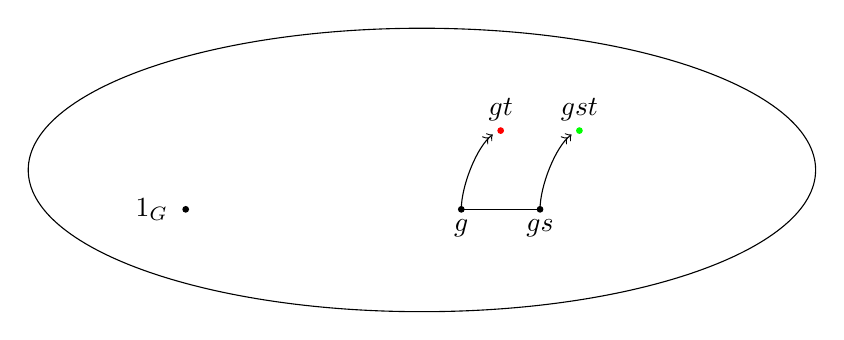
\begin{tikzpicture}

\draw (0,0) ellipse (5 and 1.8);

\filldraw [black]  (-3,-0.5) circle (1pt);

\filldraw [black] (0.5,-0.5) circle (1pt);
\filldraw [black] (1.5,-0.5) circle (1pt);
\filldraw [red] (1.0,0.5) circle (1pt);
\filldraw [green] (2.0,0.5) circle (1pt);


\draw [->>] (0.5,-0.5) .. controls (0.5,-0.2) and (0.7,0.3) .. (0.9,0.45);
\draw [->>] (1.5,-0.5) .. controls (1.5,-0.2) and (1.7,0.3) .. (1.9,0.45);

\draw (-3.1,-0.5) node[anchor=east]  {$1_G$};

\draw (0.5,-0.5) node[anchor=north] {$g$};
\draw (1.5,-0.5) node[anchor=north] {$gs$};
\draw (1.0,0.5) node[anchor=south] {$gt$};
\draw (2.0,0.5) node[anchor=south] {$gst$};
\draw (0.5,-0.5)-- (1.5,-0.5);


\end{tikzpicture}
\end{center}

All the TikZ commands can be used inline using \docAuxCommand{tikz} or within the \docAuxCommand{tikzpicture} environment. When we want to use captions and labels, we enclose it in the figure environment or use \docAuxCommand{captionof}, but it can be called anywhere in the text or math of a Tex document:

\begin{teX}
\begin{figure}
\centering
%\tikzset{external/force remake}
\begin{tikzpicture}
... TikZ commands ...
\end{tikzpicture}
\caption{A diagram drawn with TikZ.}
\label{Fig:_diagram1}
\end{figure}
\end{teX}

We can also use them in math:

\begin{teX}
\begin{align*}
\int dx\; f(x) =
\alpha
%\tikzset{external/force remake}
\begin{tikzpicture}
... TikZ commands ...
\end{tikzpicture}
\end{align*}
\end{teX}



\section{Draw simple lines}

\begin{texexample}{Draw a Line}{ex:line}

\begin{tikzpicture}
\node[draw] (S1) at (0,0) {Paris};
\node[draw] (S2) at (3,0) {Stratsbourg};
\draw (S1) -- (S2);
\end{tikzpicture}
\end{texexample}


The syntax of the command is:

|\node|\oarg{options} (\meta{name}) at (\meta{position}) |{|\meta{contents}|}|

If we look
 carefully, we see that the two writings give
Slightly different results:
- In the first case, node is an operation executed on a path. We
Can consider each node as a decoration of the point at which it
is associated. The line drawn by the draw command joins two points, the
Nodes are objects added later and centered on points. The option
Draw of the node trace operation the node outline.
- In the second case, \ node is a TikZ command which allows to define
A node, to name it and to draw it. One can then consider the
Nodes as pre-existing objects that will then be linked with the \docAuxCommand{node}.


\begin{texexample}{Draw a Line}{ex:line}
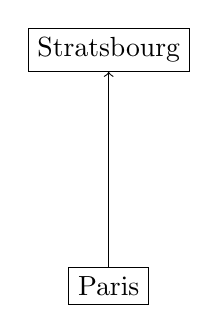
\begin{tikzpicture}
\node[draw] (S1) at (0,0) {Paris};
\node[draw] (S2) at (0,3) {Stratsbourg};
\draw[->] (S1) -- (S2);
\end{tikzpicture}
\end{texexample}

The basic building block of all pictures in \tikzname is the path. A path is a series of straight lines and curves
that are connected (that is not the whole picture, but let us ignore the complications for the moment). You
start a path by specifying the coordinates of the start position as a point in round brackets, as in (0,0).
This is followed by a series of \enquote{path extension operations.}


\begin{texexample}{Draw a Line}{ex:line}
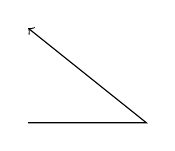
\begin{tikzpicture}
\draw[->] (0,0) -- (1.5,0) -- (0, 1.2);
\end{tikzpicture}
\end{texexample}


\subsection*{Adding Text} 

So far we have seen how to draw lines and arcs. However, an important component is still missing the addition of text. When
\tikzname is constructing a path and it encounters the keyword |node| typically followed by some options  it reads a \textit{node specification}. Options can typically follow and then it terminates by curly brackets. 
 

\begin{texexample}{Draw a Line}{ex:line}
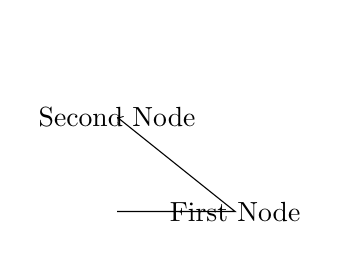
\begin{tikzpicture}
\draw[->] (0,0) -- (1.5,0) node {First Node} -- (0, 1.2) node[shape = circle] {Second Node};
\end{tikzpicture}
\end{texexample}


The \docAuxCommand*{node} can be used to abbreviate the operation. A longer example can demonstrate this better. How can we draw the following figure?

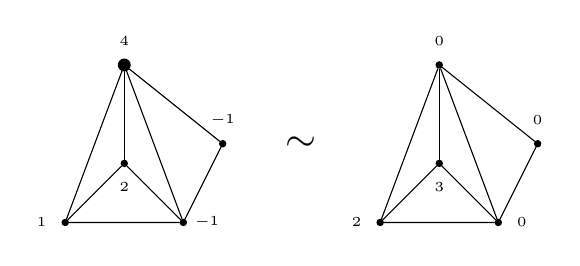
\begin{tikzpicture}
\node[circle,fill=black,inner sep=0.8pt,draw] (a) at (0,0) {};
\node[circle,fill=black,inner sep=0.8pt,draw] (b) at (1.5,0) {};
\node[circle,fill=black,inner sep=1.5pt,draw] (c) at (.75,2) {};
\node[circle,fill=black,inner sep=0.8pt,draw] (d) at (0.75,.75) {};
\node[circle,fill=black,inner sep=0.8pt,draw] (e) at (2,1) {};


\node () at (-0.3,0) {\tiny$1$};
\node () at (0.75,0.45) {\tiny$2$};
\node () at (0.75,2.3) {\tiny$4$};
\node () at (2,1.3) {\tiny$-1$};
\node () at (1.8,0) {\tiny$-1$};

\draw (a)--(b)--(e)--(c) --(a)--(d)--(b)--(c);
\draw (c)--(d);

\node at (3,1) {\Large{$\sim$}};

\begin{scope}[shift={(+4,0)}]
\node[circle,fill=black,inner sep=0.8pt,draw] (a) at (0,0) {};
\node[circle,fill=black,inner sep=0.8pt,draw] (b) at (1.5,0) {};
\node[circle,fill=black,inner sep=0.8pt,draw] (c) at (.75,2) {};
\node[circle,fill=black,inner sep=0.8pt,draw] (d) at (0.75,.75) {};
\node[circle,fill=black,inner sep=0.8pt,draw] (e) at (2,1) {};


\node () at (-0.3,0) {\tiny$2$};
\node () at (0.75,0.45) {\tiny$3$};
\node () at (0.75,2.3) {\tiny$0$};
\node () at (2,1.3) {\tiny$0$};
\node () at (1.8,0) {\tiny$0$};

\draw (a)--(b)--(e)--(c) --(a)--(d)--(b)--(c);
\draw (c)--(d);

\end{scope}
\end{tikzpicture}

\begin{texexample}{A larger example}{ex:larger}
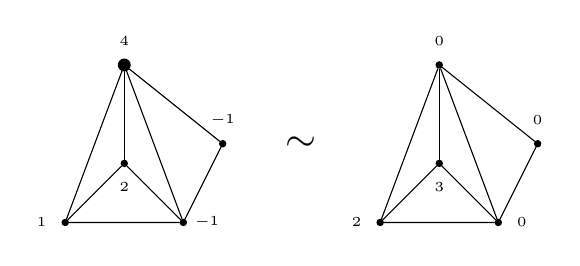
\begin{tikzpicture}
\node[circle,fill=black,inner sep=0.8pt,draw] (a) at (0,0) {};
\node[circle,fill=black,inner sep=0.8pt,draw] (b) at (1.5,0) {};
\node[circle,fill=black,inner sep=1.5pt,draw] (c) at (.75,2) {};
\node[circle,fill=black,inner sep=0.8pt,draw] (d) at (0.75,.75) {};
\node[circle,fill=black,inner sep=0.8pt,draw] (e) at (2,1) {};


\node () at (-0.3,0) {\tiny$1$};
\node () at (0.75,0.45) {\tiny$2$};
\node () at (0.75,2.3) {\tiny$4$};
\node () at (2,1.3) {\tiny$-1$};
\node () at (1.8,0) {\tiny$-1$};

\draw (a)--(b)--(e)--(c) --(a)--(d)--(b)--(c);
\draw (c)--(d);

\node at (3,1) {\Large{$\sim$}};

\begin{scope}[shift={(+4,0)}]
\node[circle,fill=black,inner sep=0.8pt,draw] (a) at (0,0) {};
\node[circle,fill=black,inner sep=0.8pt,draw] (b) at (1.5,0) {};
\node[circle,fill=black,inner sep=0.8pt,draw] (c) at (.75,2) {};
\node[circle,fill=black,inner sep=0.8pt,draw] (d) at (0.75,.75) {};
\node[circle,fill=black,inner sep=0.8pt,draw] (e) at (2,1) {};


\node () at (-0.3,0) {\tiny$2$};
\node () at (0.75,0.45) {\tiny$3$};
\node () at (0.75,2.3) {\tiny$0$};
\node () at (2,1.3) {\tiny$0$};
\node () at (1.8,0) {\tiny$0$};

\draw (a)--(b)--(e)--(c) --(a)--(d)--(b)--(c);
\draw (c)--(d);

\end{scope}
\end{tikzpicture}
\captionof{figure}{The larger vertex fires once to move from the left configuration to the right configuration.}
\end{texexample}

Behind the scenes pgf uses the basic system command \docAuxCommand{pgfnode} to create the nodes. The syntax of the command is given on \seepgfmanual{1026} as:

\begin{docCommand}{pgfnode}{\marg{shape}\marg{anchor}\marg{label text}\marg{name}\marg{path usage command}}
This command creates a new node. The \marg{shape} of the node must have been declared previously using
\lstinline{pgfdeclareshape}.

The shape is shifted such that the \marg{anchor} is at the origin. In order to place the shape somewhere else,
use the coordinate transformation prior to calling this command.
The hnamei is a name for later reference. If no name is given, nothing will be “saved” for the node, it
will just be drawn.

The \marg{path usage command} is executed for the background and the foreground path (if the shape defines
them).
\end{docCommand}


A good workflow, is to first define the nodes, next label them and then draw any connecting lines.

\begin{texexample}{Named nodes}{ex:named} 
\begin{tikzpicture}
\node[circle,fill=black,inner sep=0.8pt,draw] (a) at (0,0) {};
\node[circle,fill=black,inner sep=0.8pt,draw] (b) at (1.5,0) {};
\node[circle,fill=black,inner sep=1.5pt,draw] (c) at (.75,2) {};
\node[circle,fill=black,inner sep=0.8pt,draw] (d) at (0.75,.75) {};
\node[circle,fill=black,inner sep=0.8pt,draw] (e) at (2,1) {};
\end{tikzpicture}
\end{texexample}

\begin{texexample}{Named nodes}{ex:named} 
\begin{tikzpicture}
\node[circle,fill=black,inner sep=0.8pt,draw] (a) at (0,0) {};
\node[circle,fill=black,inner sep=0.8pt,draw] (b) at (1.5,0) {};
\node[circle,fill=black,inner sep=1.5pt,draw] (c) at (.75,2) {};
\node[circle,fill=black,inner sep=0.8pt,draw] (d) at (0.75,.75) {};
\node[circle,fill=black,inner sep=0.8pt,draw] (e) at (2,1) {};
% absolute labelling
\node () at (-0.3,0) {\tiny$1$};
\node () at (0.75,0.45) {\tiny$2$};
\node () at (0.75,2.3) {\tiny$4$};
\node () at (2,1.3) {\tiny$-1$};
\node () at (1.8,0) {\tiny$-1$};
\end{tikzpicture}
\end{texexample}

\begin{texexample}{Named nodes}{ex:named} 
\begin{tikzpicture}
\pgfdeclarelayer{background}
\pgfdeclarelayer{foreground}
\pgfsetlayers{background,main,foreground}
\node[circle,fill=black,inner sep=0.8pt,draw] (a) at (0,0) {};
\node[circle,fill=black,inner sep=0.8pt,draw] (b) at (1.5,0) {};
\node[circle,fill=black,inner sep=1.5pt,draw] (c) at (.75,2) {};
\node[circle,fill=black,inner sep=0.8pt,draw] (d) at (0.75,.75) {};
\node[circle,fill=black,inner sep=0.8pt,draw] (e) at (2,1) {};
% absolute labelling
\node () at (-0.3,0) {\tiny$1$};
\node () at (0.75,0.45) {\tiny$2$};
\node () at (0.75,2.3) {\tiny$4$};
\node () at (2,1.3) {\tiny$-1$};
\node () at (1.8,0) {\tiny$-1$};
% draw connecting lines
\draw (a)--(b)--(e)--(c) --(a)--(d)--(b)--(c);
\draw (c)--(d);
%\begin{pgfonlayer}{background}
\begin{scope}[on background layer={color=blue!10}]
\node [fill=blue!10,fit=(a) (b) (c)
(d) (e)] {};
\end{scope}
%\end{pgfonlayer}
\end{tikzpicture}
\end{texexample}

Just to recap, using \docAuxCommand*{node} and the \textbf{at} we can position accurately any node. We could have used the much longer command |path node|, but in our case above this is unecessary (\seepgfmanual{49}), for more explanations if you are still unsure.

Nodes can be named or unnamed. There are two ways to name them, with the key \docValue{name} or within brackets. The second method is to be preferred. Names for nodes can be pretty arbitrary, but they should not contain commas, periods, parentheses, colons, and some other special characters. However, they can contain underscores and hyphens

\subsection{Layers and Scope}

We can add a backround layer, using the library \textit{backgrounds}, which provides key values for adding backgrounds. \pgfname\ provides a layering mechanism for composing graphics from
multiple layers. (This mechanism is not to be confused with the
conceptual ``software layers'' the \pgfname\ system is composed of.)
Layers are often used in graphic programs. The idea is that you can
draw on the different layers in any order. So you might start drawing
something on the ``background'' layer, then something on the
``foreground'' layer, then something on the ``middle'' layer, and then
something on the background layer once more, and so on. At the end, no
matter in which ordering you drew on the different layers, the layers
are ``stacked on top of each other'' in a fixed ordering to produce
the final picture. Thus, anything drawn on the middle layer would come
on top of everything of the background layer.

Normally, you do not need to use different layers since you will have
little trouble ``ordering'' your graphic commands in such a way that
layers are superfluous. However, in certain situations you only
``know'' what you should draw behind something else after the
``something else'' has been drawn.

For example, suppose you wish to draw a yellow background behind your
picture. The background should be as large as the bounding box of the
picture, plus a little border. If you know the size of the bounding box
of the picture at its beginning, this is easy to accomplish. However,
in general this is not the case and you need to create a
``background'' layer in addition to the standard ``main'' layer. Then,
at the end of the picture, when the bounding box has been established,
you can add a rectangle of the appropriate size to the picture.

\subsection{Declaring Layers}

In \pgfname\ layers are referenced using names. The standard layer,
which is a bit special in certain ways, is called |main|. If nothing
else is specified, all graphic commands are added to the |main|
layer. You can declare a new layer using the following command:

\begin{docCommand}{pgfdeclarelayer}{\marg{name}}
  This command declares a layer named \meta{name} for later
  use. Mainly, this will set up some internal bookkeeping.
\end{docCommand}

The next step toward using a layer is to tell \pgfname\ which layers
will be part of the actual picture and which will be their
ordering. Thus, it is possible to have more layers declared than are
actually used.

\begin{docCommand}{pgfsetlayers}{\marg{layer list}}
  This command tells \pgfname\ which layers will be used in
  pictures. They are stacked on top of each other in the order
  given. The layer |main| should always be part of the list. Here is
  an example:
\begin{codeexample}[code only]
\pgfdeclarelayer{background}
\pgfdeclarelayer{foreground}  
\pgfsetlayers{background,main,foreground}
\end{codeexample}

  This command should be given either outside of any picture or ``directly inside'' of a picture.
  Here, the ``directly inside'' means that there should be no further level of \TeX\ grouping between |\pgfsetlayers| and the matching |\end{pgfpicture}| (no closing braces, no |\end{...}|). It will also work if |\pgfsetlayers| is provided before |\end{tikzpicture}| (with similar restrictions).
\end{docCommand}


\subsection{Using Layers}

Once the layers of your picture have been declared, you can start to
``fill'' them. As said before, all graphics commands are normally
added to the |main| layer. Using the |{pgfonlayer}| environment, you
can tell \pgfname\ that certain commands should, instead, be added to
the given layer.

\begin{docEnvironment}{pgfonlayer}{\marg{layer name}}
\end{docEnvironment}

The whole \meta{environment contents} is added to the layer with the
name \meta{layer name}. This environment can be used anywhere inside
a picture. Thus, even if it is used inside a |{pgfscope}| or a \TeX\
group, the contents will still be added to the ``whole'' picture.
Using this environment multiple times inside the same picture will
cause the \meta{environment contents} to accumulate.

  \emph{Note:} You can \emph{not} add anything to the |main| layer
  using this environment. The only way to add anything to the main
  layer is to give graphic commands outside all |{pgfonlayer}|
  environments. 



\begin{codeexample}[]
\pgfdeclarelayer{background layer}
\pgfdeclarelayer{foreground layer}
\pgfsetlayers{background layer,main,foreground layer}
\begin{tikzpicture}
  % On main layer:
  \fill[blue] (0,0) circle (1cm);
  
  \begin{pgfonlayer}{background layer}
    \fill[yellow] (-1,-1) rectangle (1,1);
  \end{pgfonlayer}
  
  \begin{pgfonlayer}{foreground layer}
    \node[white] {foreground};
  \end{pgfonlayer}
  
  \begin{pgfonlayer}{background layer}
    \fill[black] (-.8,-.8) rectangle (.8,.8);
  \end{pgfonlayer}

  % On main layer again:
  \fill[blue!50] (-.5,-1) rectangle (.5,1);
\end{tikzpicture}
\end{codeexample}



\long\gdef\mytriangle{
\node[circle,fill=black,inner sep=0.8pt,draw] (a) at (0,0) {};
\node[circle,fill=black,inner sep=0.8pt,draw] (b) at (1.5,0) {};
\node[circle,fill=black,inner sep=1.5pt,draw] (c) at (.75,2) {};
\node[circle,fill=black,inner sep=0.8pt,draw] (d) at (0.75,.75) {};
\node[circle,fill=black,inner sep=0.8pt,draw] (e) at (2,1) {};
% absolute labelling
\node () at (-0.3,0) {\tiny$1$};
\node () at (0.75,0.45) {\tiny$2$};
\node () at (0.75,2.3) {\tiny$4$};
\node () at (2,1.3) {\tiny$-1$};
\node () at (1.8,0) {\tiny$-1$};
% draw connecting lines
\draw (a)--(b)--(e)--(c) --(a)--(d)--(b)--(c);
\draw (c)--(d);
}

\begin{texexample}{Adding backgrouns}{ex:backgrounds}
\begin{tikzpicture}
\pgfdeclarelayer{background}
\pgfdeclarelayer{foreground}
\pgfsetlayers{background,main,foreground}
\mytriangle
%\begin{pgfonlayer}{background}
\begin{scope}[on background layer={color=blue!10}]
\mytriangle
\node [fill=blue!10,fit=(a) (b) (c)
(d) (e)] {};
\end{scope}
%\end{pgfonlayer}
\end{tikzpicture}
\end{texexample}


\begin{texexample}{Adding backgrouns}{ex:backgrounds}
\begin{tikzpicture}
\pgfdeclarelayer{background}
\pgfdeclarelayer{foreground}
\pgfsetlayers{background,main,foreground}
\mytriangle
%\begin{pgfonlayer}{background}
\begin{scope}[on background layer={color=blue!10}]
\node [fill=blue!10,fit=(a) (b) (c)
(d) (e)] {};
\end{scope}

\begin{scope}[shift={(+4,0)}]
\mytriangle
\begin{pgfonlayer}{background}
\node [pattern=checkerboard light gray,fit=(a) (b) (c)
(d) (e)] {};
\end{pgfonlayer}
\end{scope}
\end{tikzpicture}
\end{texexample}

This brings us to the end of our discussion. Time for a coffee and a break.                

\section{Adding styles}

In our previous example, we cut and pasted many of the repetitive keys. \pgfname offers a way to set a new key to the values of other keys using the handler |.style|. This is a very powerful way of redefining new keys, but also simplifying the code. Styles in \tikzname can be considered similar to macros in standard LaTeX. When I made a drawing, we can still tweak the styles and look how the drawing changes, until it's perfect. You should never have to tweak each node.

\begin{texexample}{Using styles}{ex:usingstyles}
\tikzset{BN/.style = {circle,fill=black,inner sep=0.8pt,draw},
         tiny/.style = {font=\tiny}, 
}
\begin{tikzpicture}
\node[BN] (a) at (0,0) {};
\node[BN] (b) at (1,0) {};
\node[BN] (c) at (1,1) {};
\node[BN] (d) at (0,1) {};
\node[BN] (e) at (-1,0) {};

\node () at (-1.3,0) [tiny]{$v_1$};
\node () at (-.3,1)  [tiny]{$v_2$};
\node () at (1.3,0)  [tiny]{$w_1$};
\node () at (1.3,1)  [tiny]{$w_2$};

\node[tiny] () at (0.5,-0.2) {$a$};
\node[tiny] () at (0.5,1.2) {$b$};
\node[tiny] () at (0.2,0.5) {$c$};
\node[tiny] () at (-0.5,-.2) {$d$};

\draw (e) -- (a) -- (b) -- (c) -- (d) -- (a);
\draw (e) -- (d);

\end{tikzpicture}
\end{texexample}



\section{Arcs and options for lines}

\begin{texexample}{Draw a Line}{ex:line}
\begin{tikzpicture}
\draw[->] (0,0) -- (1.5,0) node[draw, ellipse] {First Node} -| (0, 1.2) node[draw,ellipse,rotate=45] {Second Node};
\end{tikzpicture}
\end{texexample}

\begin{texexample}{Drawing arcs}{ex:matharcs}
We define 
\begin{gather*}
    \bar{d}_{k,l}:=\hspace{6pt}
    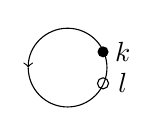
\begin{tikzpicture}[baseline=(current bounding box.center)]
    \draw[->] (3,2) arc (-180:180:5mm);
	  \fill (3.95,2.2) circle [radius=2pt];
    \draw (3.95,1.8) circle [radius=2pt];
    \node at (4.2,1.8) {$l$};
    \node at (4.2,2.2) {$k$};
    \end{tikzpicture}
    \hspace{0.5cm}
    \text{and}
    \hspace{0.5cm}
    d_{k,l}:=\hspace{6pt}
    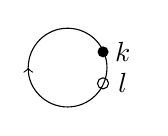
\begin{tikzpicture}[baseline=(current bounding box.center)]
    \draw[<-] (3,2) arc (-180:180:5mm);
    \fill (3.95,2.2) circle [radius=2pt];
    \draw (3.95,1.8) circle [radius=2pt];
    \node at (4.2,1.8) {$l$};
    \node at (4.2,2.2) {$k$};
    \end{tikzpicture}
    \hspace{0.5cm}
    \text{for}
    \hspace{2mm} k,l\in\mathbb{Z}_{\geq 0}.
\end{gather*}
\end{texexample}


Here is a figure that you should try and reproduce.
\newcommand{\G}{\Gamma}

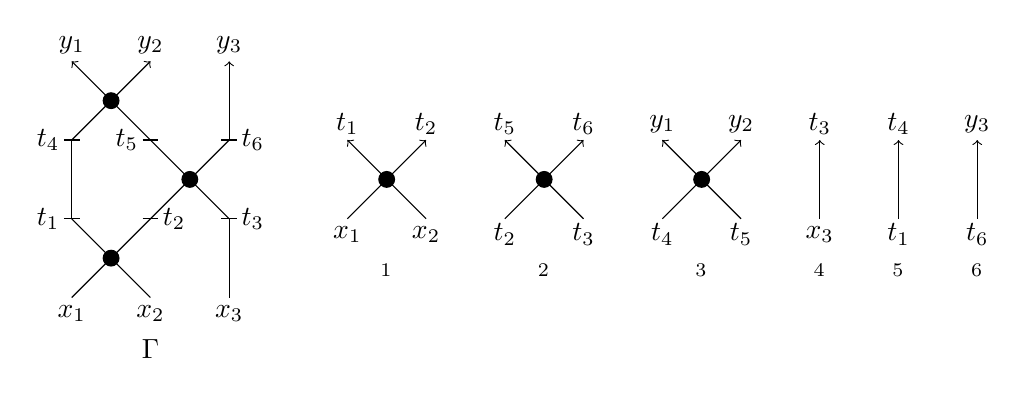
\begin{tikzpicture}
\draw (-3.5,-1)--(-2.5,0); \draw (-2.5,-1)--(-3.5,0); \draw (-1.5,-1)--(-1.5,0);\draw[fill=black] (-3,-0.5) circle (0.1cm); \draw (-3.5,0)--(-3.5,1); \draw (-2.5,0)--(-1.5,1); \draw (-1.5,0)--(-2.5,1);\draw[fill=black] (-2,0.5) circle (0.1cm); \draw[->] (-3.5,1)--(-2.5,2); \draw[->] (-2.5,1)--(-3.5,2); \draw[->] (-1.5,1)--(-1.5,2); \draw[fill=black] (-3,1.5) circle (0.1cm); \draw (-3.6,0)--(-3.4,0);\draw (-2.6,0)--(-2.4,0);\draw (-1.6,0)--(-1.4,0); \draw (-3.6,1)--(-3.4,1);\draw (-2.6,1)--(-2.4,1);\draw (-1.6,1)--(-1.4,1); \node at (-3.5,-1.2) {$x_1$};\node at (-2.5,-1.2) {$x_2$};\node at (-1.5,-1.2) {$x_3$}; \node at (-3.5,2.2) {$y_1$};\node at (-2.5,2.2) {$y_2$};\node at (-1.5,2.2) {$y_3$}; \node at (-3.8,0) {$t_1$};\node at (-2.2,0) {$t_2$};\node at (-1.2,0) {$t_3$}; \node at (-3.8,1) {$t_4$};\node at (-2.8,1) {$t_5$};\node at (-1.2,1) {$t_6$}; \node at (-2.5,-1.65) {$\Gamma$};
\draw[->] (0,0)--(1,1); \draw[->] (1,0)--(0,1); \draw[fill=black] (0.5,0.5) circle (0.1cm); \draw[->] (2,0)--(3,1); \draw[->] (3,0)--(2,1); \draw[fill=black] (2.5,0.5) circle (0.1cm); \draw[->] (4,0)--(5,1); \draw[->] (5,0)--(4,1); \draw[fill=black] (4.5,0.5) circle (0.1cm); \draw[->] (6,0)--(6,1); \draw[->] (7,0)--(7,1); \draw[->] (8,0)--(8,1);
\node at (0,-.2) {$x_1$};\node at (1,-.2) {$x_2$}; \node at (2,-.2) {$t_2$};\node at (3,-.2) {$t_3$}; \node at (4,-.2) {$t_4$};\node at (5,-.2) {$t_5$}; \node at (6,-.2) {$x_3$}; \node at (7,-.2) {$t_1$}; \node at (8,-.2) {$t_6$};
\node at (0,1.2) {$t_1$};\node at (1,1.2) {$t_2$}; \node at (2,1.2) {$t_5$};\node at (3,1.2) {$t_6$}; \node at (4,1.2) {$y_1$};\node at (5,1.2) {$y_2$}; \node at (6,1.2) {$t_3$}; \node at (7,1.2) {$t_4$}; \node at (8,1.2) {$y_3$};
\node at (0.5,-0.65) {$\G_1$}; \node at (2.5,-0.65) {$\G_2$}; \node at (4.5,-0.65) {$\G_3$}; \node at (6,-0.65) {$\G_4$};\node at (7,-0.65) {$\G_5$};\node at (8,-0.65) {$\G_6$}; 
\end{tikzpicture}

This brings us to the end.




The |node| can take numerous options who are then used to set the typesetting of the text that follows:


\begin{texexample}{Draw a Line}{ex:line}
\begin{tikzpicture}
\draw[->] (0,0) -- (1.5,0) node[draw, ellipse] {First Node} -| (0, 1.2) node[draw,ellipse,rotate=45, text width=3cm, fill=creamy, text justified] {\lorem};
\end{tikzpicture}
\end{texexample}


\begin{texexample}{Draw a Line}{ex:line}
\begin{tikzpicture}[funny ellipse/.style = {draw,ellipse,rotate=45, text width=3cm, fill=creamy, text justified} ]
\draw[->] (0,0) -- (1.5,0) node[draw, ellipse] {First Node} -| (0, 1.2) node[funny ellipse] {\lorem};
\end{tikzpicture}
\end{texexample}

This can also be written by using \docAuxCommand{tikzset} for setting out all the keys. This can written just before the environment or within the scope of the environment. See \href{https://tex.stackexchange.com/questions/52372/should-tikzset-or-tikzstyle-be-used-to-define-tikz-styles}{TX.SX discussion}, for the option to set |\tikzstyle| which should not be used, even if it is quicker to write.


\begin{texexample}{Draw a Line}{ex:line}
\tikzset{funny ellipse/.style = {draw,ellipse,rotate=45, text width=3cm, fill=creamy, text justified} }
\begin{tikzpicture}
\draw[->] (0,0) -- (1.5,0) node[draw, ellipse] {First Node} -| (0, 1.2) node[funny ellipse] {\lorem};
\end{tikzpicture}
\end{texexample}

A |node| can possibly be rendered with a choice from a list of over 720 keys.

ed. 



Using the |TikZ| package you can draw figures and intermingle them with text. To draw a simple diamond as shown in \fref{fig:diamond} we use
the following commands. The package comes with a very comprehensive manual of over 500 pages long. One can state that there is nothing that you cannot draw with PGF/TikZ, if you have the patience and perseverance. TikZ's language has a syntax of its own with very little connection to what we have used so far. You will need to set aside adequate time to study this, especially if your work has a lot of specially drawn figures that you need. The result like anything else in \tex make the effort worthwhile.

\begin{texexample}{Draw a Diamond}{fig:diamond}

\begin{tikzpicture}
 \draw (1,0) -- (0,1) -- (-1,0) -- (0,-1) -- cycle;
\end{tikzpicture}
\end{texexample}


\begin{texexample}{Text long path}{ex:decorations}
\begin{tikzpicture}
\draw [help lines] grid (3,2);
\draw [red, dashed]
[postaction={decoration={text along path, text={a big juicy apple},
text align=fit to path}, decorate}]
(0,0) .. controls (0,2) and (3,2) .. (3,0);
\node (A) at (1.5,0) {!};
\end{tikzpicture}
\end{texexample}


\begin{texexample}{Text long path}{ex:decorations}

Hello \begin{pgfpicture}
\pgfpathrectangle{\pgfpointorigin}{\pgfpoint{2ex}{1ex}}
\pgfusepath{stroke}
\end{pgfpicture} World!

\end{texexample}


\emphasis{-,draw,begin,end,tikzpicture}
\begin{teXXX}

\begin{tikzpicture}
\draw (1,0) -- (0,1) -- (-1,0) -- (0,-1) -- cycle;
\end{tikzpicture}
\end{teXXX}



\makeatletter
The value of $x$ is \pgfsys@markposition{here}important.

Lots of text.
\hbox{\pgfsys@markposition{myorigin}%
\begin{pgfpicture}
% Switch of size protocol
\pgfpathmoveto{\pgfpointorigin}
\pgfusepath{use as bounding box}
\pgfsys@getposition{here}{\hereposition}
\pgfsys@getposition{myorigin}{\thispictureposition}
\pgftransformshift{\pgfpointscale{-1}{\thispictureposition}}
\pgftransformshift{\hereposition}
\pgfpathcircle{\pgfpointorigin}{1cm}
\pgfusepath{draw}
\end{pgfpicture}}

\makeatother


You cannot write directly into a picture environment. The command \docAuxCommand{pgftext} can be used. 

\begin{texexample}{Using text directly}{ex:pgftext}
\tikz{\draw[help lines] (0,0) grid (3,2);
\pgftext[base,x=1cm,y=0.5cm] {lovely}}
\end{texexample}





Sometimes it is quite useful when debugging to add a backround grid. 


\begin{centering}
\begin{tikzpicture}
\draw[step=0.25cm,color=creamy] (-1,-1) grid (1,1);
\draw [color=bgsexy](1,0) -- (0,1) -- (-1,0) -- (0,-1) -- cycle;
\end{tikzpicture}
\captionof{figure}{You can add a background grid using \texttt{step=0.25cm, color=green} as an option}
\end{centering}


\emphasis{step,color,green,grid,begin,end}
\begin{teXXX}
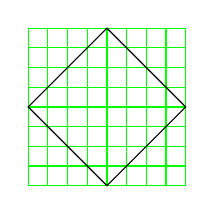
\begin{tikzpicture}
  \draw[step=0.25cm,color=green] (-1,-1) grid (1,1);
  \draw (1,0) -- (0,1) -- (-1,0) -- (0,-1) -- cycle;
\end{tikzpicture}
\end{teXXX}

The grid is specified by providing two diagonally opposing points: (-1,-1)
and (1, 1). The two options supplied give a step size for the grid lines and a
specification for the color of the grid lines, using the \docpkg{xcolor} package

\subsection{Specifying points and paths}

\begin{texexample}{Specifying points and paths}{ex:points}
\centering
\begin{tikzpicture}[scale=1.8]
% Define the points of a regular pentagon
\path (0,0) coordinate (origin);
\path (0:1cm) coordinate (P0);
\path (1*72:1cm) coordinate (P1);
\path (2*72:1cm) coordinate (P2);
\path (3*72:1cm) coordinate (P3);
\path (4*72:1cm) coordinate (P4);
% Draw the edges of the pentagon
\draw[color=bgsexy] (P0) -- (P1) -- (P2) -- (P3) -- (P4) -- cycle;
% Add "spokes"
\draw[color=red800] (origin) -- (P0) (origin) -- (P1) (origin) -- (P2)
(origin) -- (P3) (origin) -- (P4);
\end{tikzpicture}
\captionof{figure}{Drawing a complicated polygon, using paths and the \texttt{draw} command}
\end{texexample}


Two key ideas used in \tikzname\ are points and paths. Both of these ideas were used
in the diamond examples. Much more is possible, however. For example, points
can be specified in any of the following ways:
\begin{enumerate}
\item  Cartesian coordinates
\item  Polar coordinates
\item  Named points
\item  Relative points
\end{enumerate}



\subsection{coordinates}
The cartesian coordinates can be defined and named using the following syntax.

%\emphasis{begin,end,coordinate,at,draw}
%\begin{teXXX}
%\begin{tikzpicture}
%  \coordinate (A) at (0,0);
%  \coordinate (B) at (1.25,0.25);
%  \draw[blue] (A) -- (B);
%\end{tikzpicture}
%\end{teXXX}

\noindent This produces:
\begin{tikzpicture}
\coordinate (A) at (0,0);
\coordinate (B) at (1.25,0.25);
\draw[blue] (A) -- (B);
\end{tikzpicture}


We can add labels to the points by using the |label| option. A label is distinct from the text of a |node|.

\begin{tikzpicture}
\coordinate [label=left:\textcolor{orange}{$A$}] (A) at (0,0);
\coordinate [label=right:\textcolor{orange}{$B$}]  (B) at (1.15,0.25);
\draw[blue] (A) -- (B);
\end{tikzpicture}

\emphasis{label,left,label:,right}
\begin{teXXX}
\begin{tikzpicture}
  \coordinate [label=left:\textcolor{orange}{$A$}] (A) at (0,0);
  \coordinate [label=west:\textcolor{orange}{$B$}] (B) at (1.25,0.25);
  \draw[blue] (A) -- (B);
\end{tikzpicture}
\end{teXXX}




If you tempted to write \texttt{label=top:} it will not work, as the command accepts the following keywords.


\begin{tikzpicture}
  \coordinate [label=left:\textcolor{orange}{east}]  (A) at (0,0);
  \coordinate [label=right:\textcolor{orange}{west}] (B) at (0,0);
  \draw[blue] (A)--(B);
\end{tikzpicture}


\section{Graphic Parameters: Line Width, Line Cap, and Line Join}

The width of lines can be specified using the key:

\begin{docKey}[tikz]{line width}{=\marg{dimension}} {no default, initially 0.4pt}
Specifies the line width \seepgfmanual{166}
\end{docKey}



\bgroup
\def\mkl#1{\tikz \draw[#1] (0,0)--(1.0, 1.5ex);}
\scriptsize\arial
\begin{tabular}{|l|l|l|l|l|l|l|l|}
\hline
\mkl{line width=2pt}& \mkl{ultra thin} &\mkl{very thin} & \mkl{thin} & \mkl{semithick} & \mkl{thick} &\mkl{very thick} &\mkl{ultra thick} \\
\hline
line width=2pt &ultra thin & very thin & thin &semithick & thick & very thick & ultra thick \\
\hline
\end{tabular}
\egroup

\begin{docKey}[tikz]{line cap}{=\marg{dimension}} {no default, initially 0.4pt}
Specifies how lines “end.” Permissible types are round, rect, and butt \seepgfmanual{167}. 
\end{docKey}

\bgroup
\def\mkl#1{\begin{tikzpicture} \draw[line width=10pt, line cap=#1] (0,0)--(1.0, 1.5ex);\draw[white,line width=2pt]
(0,0 )--(1.0,1.5ex);\end{tikzpicture}}
\scriptsize\arial
\begin{tabular}{|l|l|l|}
\hline
\mkl{rect}& \mkl{butt} &\mkl{round}  \\
\hline
rect &butt & round \\
\hline
\end{tabular}
\egroup




\begin{docKey}[tikz]{line join}{=\marg{type}}{no default, initially miter}
Specifies how lines “join.” Permissible type are round, bevel, and miter. They have the following
effects:
\end{docKey}

\begin{texexample}{Joining Lines}{es:joinlines}

\begin{tikzpicture}[line width=10pt]
\draw[line join=round] (0,0) -- ++(.5,1) -- ++(.5,-1);
\draw[line join=bevel] (1.25,0) -- ++(.5,1) -- ++(.5,-1);
\draw[line join=miter] (2.5,0) -- ++(.5,1) -- ++(.5,-1);
\end{tikzpicture}
\end{texexample}


\begin{docKey}[tikz]{dash pattern}{=\marg{dash pattern}}{no default}
Sets the dashing pattern. The syntax is the same as in \metafontlogo. For example following pattern on
2pt off 3pt on 4pt off 4pt means \enquote{draw 2pt, then leave out 3pt, then draw 4pt once more, then
leave out 4pt again, repeat}.
\end{docKey}

\bgroup
\def\ml#1{\tikz \draw[ #1] (0pt,0pt) -- (50pt,0pt);}
\def\alist{solid, dotted, densely dotted, loosely dotted,% 
           dashed,densely dashed, loosely dashed, %
           dash dot, densely dash dot, loosely dash dot, %
           dash dot dot, densely dash dot dot, loosely dash dot dot.}

For patterns there are numerous settings {\arial \alist }


\scriptsize
\begin{tabular}{lll}
\hline
\ml{solid} &  & \\
solid      &  & \\
\hline
\ml{dotted} &\ml{densely dotted} & \ml{loosely dotted}\\
\textit{dotted} & densely dotted  &loosely dotted \\
\hline
\ml{dashed} & \ml{densely dashed} & \ml{loosely dashed}  \\
\textit{dashed}      & densely dashed & loosely dashed            \\
\hline

\ml{dash dot} & \ml{densely dash dot} & \ml{loosely dash dot} \\
\textit{dash dot} & densely dash dot & loosely dash dot \\
\hline

\ml{dash dot dot} & \ml{densely dash dot dot} & \ml{loosely dash dot dot} \\
\textit{dash dot dot} & densely dash dot dot & loosely dash dot dot \\
\hline
\end{tabular}
\egroup


\subsection{Pattern Library}

The library patterns can be used to draw predetermined patterns. This will be a longer than usual section as it explains how to create new patterns. Most of the content is straight from the \pgfname manual. Before we start with the creation f a new pattern let us examine how a pattern is used.

\begin{texexample}{Using Library Patterns}{ex:libpatterns}
\begin{tikzpicture}
\pattern [path fading=west,pattern=checkerboard light gray]
      (0,0) rectangle (5cm,2em);
\end{tikzpicture}
\end{texexample}


\label{section-library-patterns}


The package defines patterns for filling areas. \docAuxCommand*{usetikzlibrary}\marg{patterns}.




\subsection{Form-Only Patterns}

\begin{tabular}{ll}
  \emph{Pattern name} & \emph{Example (pattern in black, blue, and red
    on faded checkerboard)} \\ 
  \patternindex{horizontal lines} 
  \patternindex{vertical lines} 
  \patternindex{north east lines} 
  \patternindex{north west lines} 
  \patternindex{grid} 
  \patternindex{crosshatch} 
  \patternindex{dots} 
  \patternindex{crosshatch dots} 
  \patternindex{fivepointed stars} 
  \patternindex{sixpointed stars} 
  \patternindex{bricks}
  \patternindex{checkerboard}
\end{tabular}
  
\subsection{Inherently Colored Patterns}


\begin{tabular}{ll}
  \emph{Pattern name} & \emph{Example} \\
  \patternindexinherentlycolored{checkerboard light gray} 
  \patternindexinherentlycolored{horizontal lines light gray} 
  \patternindexinherentlycolored{horizontal lines gray} 
  \patternindexinherentlycolored{horizontal lines dark gray} 
  \patternindexinherentlycolored{horizontal lines light blue} 
  \patternindexinherentlycolored{horizontal lines dark blue} 
  \patternindexinherentlycolored{crosshatch dots gray} 
  \patternindexinherentlycolored{crosshatch dots light steel blue} 
\end{tabular}
  


% Copyright 2006 by Till Tantau
%
% This file may be distributed and/or modified
%
% 1. under the LaTeX Project Public License and/or
% 2. under the GNU Free Documentation License.
%
% See the file doc/generic/pgf/licenses/LICENSE for more details.


\section{Creating Patterns}

\label{section-patterns}

\subsection{Overview}

There are many ways of filling a path. First, you can fill it using a
solid color and this is also the fastest method. Second, you can also
fill it using a shading, which means that the color changes smoothly
between two (or more) different colors. Third, you can fill it using a
tiling pattern and it is explained in the following how this is done.

A tiling pattern can be imagined as a rectangular tile (hence the
name) on which a small picture is painted. There is not a single tile,
but (conceptually) an infinite number of tiles, all showing the same
picture, and these tiles are arranged horizontally and vertically to
fill the plane. When you use a tiling pattern to fill a path, what
happens is that the path clips out a ``window'' through which we see
part of this infinite plane.

Patterns come in two versions: \emph{inherently colored patterns} and
\emph{form-only patterns}. (These are often called ``color patterns''
and ``uncolored patterns,'' but these names are misleading since
uncolored patterns do have a color and the color changes. As I said,
the name is misleading\dots) An inherently colored pattern is just a
colored tile like, say, a red star with a black outline. A form-only
pattern can be imagined as a tile that is a kind of rubber stamp. When
this pattern is used, the stamp is used to print copies of the stamp
picture onto the plane, but we can use a different stamp color each
time we use a form-only pattern.

\pgfname\ provides a special support for patterns. You can declare a
pattern and then use it very much like a fill color. \pgfname\
directly maps patterns to the pattern facilities of the underlying
graphic languages (PostScript, \textsc{pdf}, and \textsc{svg}). This
means that filling a path using a pattern will be nearly as fast as if
you used a uniform color.

There are a number of pitfalls and restrictions when using
patterns. First, once a pattern has been declared, you cannot change
it anymore. In particular, it is not possible to enlarge it or change
the line width. Such flexibility would require that the repeating of
the pattern were not done by the graphic language, but on the
\pgfname\ level. This would make patterns orders of magnitude slower
to produce and to render. However, \pgfname{} does provide a
more-or-less successful emulation of ``mutable'' patterns, although
internally, a new (fixed) instance of a pattern is declared when
the parameters of a pattern change.

Second, the phase of patterns is not well-defined, that is, it is not
clear where the origin of the ``first'' tile is. To be more precise,
PostScript and \textsc{pdf} on the one hand and \textsc{svg} on the
other hand define the origin differently. PostScript and \textsc{pdf}
define a fixed origin that is independent of where the path lies. This
has the highly desirable effect that if you use the same pattern to
fill multiple paths, the outcome is the same as if you had filled a 
single path consisting of the union of all these paths. By
comparison, \textsc{svg} uses the upper-left (?) corner of the path to
be filled as the origin. However, the \textsc{svg} specification is a
bit vague on this question.


\subsection{Declaring a Pattern}

Before a pattern can be used, it must be declared. The following
command is used for this:

\begin{docCommand}{pgfdeclarepatternformonly}{%
	\oarg{variables}%
	\marg{name}%
	\marg{bottom left}%
	\marg{top right}%
	\marg{tile size}%
	\marg{code}}

	This command declares a new form-only pattern. The \meta{name} is a
  name for later reference. The two parameters \meta{lower left} and
  \meta{upper right} must describe a bounding box that is large enough
  to encompass the complete tile.
\end{docCommand}

  The size of a tile is given by \meta{tile size}, that is, a tile is
  a rectangle whose lower left   corner is the origin and whose upper
  right corner is given by \meta{tile size}. This might make you
  wonder why the second and third parameters are needed. First, the
  bounding box might be smaller than the tile size if the tile is
  larger than the picture on the tile. Second, the bounding box might
  be bigger, in which case the picture will ``bleed'' over the tile.

  The \meta{code} should be \pgfname\ code than can be protocolled. It
  should not contain any color code.


\begin{codeexample}[]
\pgfdeclarepatternformonly{stars}
{\pgfpointorigin}{\pgfpoint{1cm}{1cm}}
{\pgfpoint{1cm}{1cm}}
{
  \pgftransformshift{\pgfpoint{.5cm}{.5cm}}
  \pgfpathmoveto{\pgfpointpolar{0}{4mm}}
  \pgfpathlineto{\pgfpointpolar{144}{4mm}}
  \pgfpathlineto{\pgfpointpolar{288}{4mm}}
  \pgfpathlineto{\pgfpointpolar{72}{4mm}}
  \pgfpathlineto{\pgfpointpolar{216}{4mm}}
  \pgfpathclose%
  \pgfusepath{fill}
}
\begin{tikzpicture}
  \filldraw[pattern=stars] (0,0)   rectangle (1.5,2);
  \filldraw[pattern=stars,pattern color=red]
                           (1.5,0) rectangle (3,2);
\end{tikzpicture}
\end{codeexample}

	The optional argument \meta{variables} consists of a comma
	separated	list of macros,	registers or keys, representing the
	parameters of the pattern that may vary. If a variable is a key,
	then the full path name must be used (specifically, it must start
	with |/|).
	As an example, a list might look like the following:
	|\mymacro,\mydimen,/pgf/my key|. Note that macros and keys should
	be ``simple''. They should only store values in themselves.
	
	The effect of \meta{variables}, is the following:
  Normally, when this argument is empty, once a pattern has been
  declared, it becomes ``frozen''. This means that it is not possible
  to enlarge the pattern or change the line width later on.
  By specifying \meta{variables}, no pattern is actually created.
  Instead, the arguments are stored away
  (so the macros,	registers or keys do not have to be defined in advance).

  When the fill pattern is set, \pgfname{} checks if the pattern has
  already been created with the \meta{variables} set to their current
  values (\pgfname{} is usually ``smart enough'' to distinguish between
  macros, registers and keys). If so, this already-declared-pattern
  is used as the fill pattern.
  If not, a new instance of the pattern (which will have a
  unique internal name) is declared using the current values of
  \meta{variables}. These values are then saved and the fill pattern
  set accordingly.
	
	The following shows an example of a pattern which varies
	according to the values of the macro |\size|, the key |/tikz/radius|,
	and the \TeX{} dimension |\thickness|.

\begin{texexample}{New Pattern Example}{ex:newpattern}
\pgfdeclarepatternformonly[/tikz/radius,\thickness,\size]{rings}
{\pgfpoint{-0.5*\size}{-0.5*\size}}
{\pgfpoint{0.5*\size}{0.5*\size}}
{\pgfpoint{\size}{\size}}
{
  \pgfsetlinewidth{\thickness}
  \pgfpathcircle\pgfpointorigin{\pgfkeysvalueof{/tikz/radius}}
  \pgfusepath{stroke}
}
\newdimen\thickness
\tikzset{
  radius/.initial=4pt,
  size/.store in=\size, size=20pt,
  thickness/.code={\thickness=#1},
  thickness=0.75pt
}
\begin{tikzpicture}[rings/.style={pattern=rings}]
  \filldraw [rings, radius=2pt, size=6pt]      (0,0)   rectangle +(1.5,2);
  \filldraw [rings, radius=2pt, size=8pt]      (2,0)   rectangle +(1.5,2);
  \filldraw [rings, radius=6pt, thickness=2pt] (0,2.5) rectangle +(1.5,2);
  \filldraw [rings, radius=8pt, thickness=4pt] (2,2.5) rectangle +(1.5,2);
\end{tikzpicture}
\end{texexample}



\begin{docCommand}{pgfdeclarepatterninherentlycolored}{\oarg{variables}
    \marg{name}
    \marg{lower left}
    \marg{upper right}
    \marg{tile size}
    \marg{code}}
  This command works like |\pgfdeclarepatternuncolored|, only the
  pattern will have an inherent color. To set the color, you should
  use \pgfname's color commands, not the |\color| command, since this
  fill is not protocolled.
\end{docCommand}

\begin{texexample}{Inherently Colored}{ex:ingerentlycolored}
\pgfdeclarepatterninherentlycolored{green stars}
{\pgfpointorigin}{\pgfpoint{1cm}{1cm}}
{\pgfpoint{1cm}{1cm}}
{
  \pgfsetfillcolor{green!50!black}
  \pgftransformshift{\pgfpoint{.5cm}{.5cm}}
  \pgfpathmoveto{\pgfpointpolar{0}{4mm}}
  \pgfpathlineto{\pgfpointpolar{144}{4mm}}
  \pgfpathlineto{\pgfpointpolar{288}{4mm}}
  \pgfpathlineto{\pgfpointpolar{72}{4mm}}
  \pgfpathlineto{\pgfpointpolar{216}{4mm}}
  \pgfpathclose%
  \pgfusepath{stroke,fill}
}
\begin{tikzpicture}
  \filldraw[pattern=green stars] (0,0) rectangle (3,2);
\end{tikzpicture}
\end{texexample}



\subsection{Setting a Pattern}

Once a pattern has been declared, it can be used.

\begin{docCommand}{pgfsetfillpattern}{\marg{name}\marg{color}}
  This command specifies that paths that are filled should be filled
  with the ``color'' by the pattern \meta{name}. For an inherently
  colored pattern, the \meta{color} parameter is ignored. For
  form-only patterns, the \meta{color} parameter specifies the color
  to be used for the pattern.
\end{docCommand}
  
\begin{codeexample}[]
\begin{tikzpicture}
  \pgfsetfillpattern{stars}{red}
  \filldraw (0,0) rectangle (1.5,2);

  \pgfsetfillpattern{green stars}{red}
  \filldraw (1.5,0) rectangle (3,2);
\end{tikzpicture}
\end{codeexample}



\endinput
%To summarize, what we have been doing so far is to learn a set of primitive TikZ commands for drawing paths, drawing shapes and labeling them. All TikZ command work by passing options to them. For example to change the above line to an arrow, we just pass the option |->| to the |draw| command.
%

%\begin{tikzpicture}
%  \coordinate [label=left:\textcolor{orange}{$A$}] (A) at (0,0);
%  \coordinate [label=right:\textcolor{orange}{$B$}] (B) at (1.25,0.25);
%  \draw[->,o-stealth] (A)--(B);
%\end{tikzpicture}
%\caption{Effect of the option \protect\texttt{draw[->]}.}

%\emphasis{begin,end,->,draw}
%\begin{teXXX}
%\begin{tikzpicture}
%  ...
%  ...
%  \draw[->,blue] (A)--(B);
%\end{tikzpicture}
%\end{teXXX}
%
%\section*{Relative coordinates}
%\index{TikZ!coordinates, relative}
%A coordinate can be made "relative" by prefixing it with |++|. relative coordinates are useful in many applications.
%\medskip
%
%\noindent The code is simple, except before the coordinate you add the |++| signs. This tells the PGF engine to add the x,y dimensions of the new coordinate to that of its predecessor's. In many instances this is more intuitive and easier to determine.



%\begin{tikzpicture}
%\draw[step=0.5cm,color=gray] (-1,-1) grid (3.5,3);
%\draw[->,red,thick] (0,0) -- ++(1,0) -- ++(0,1) -- ++(-1,0) -- cycle;
%\draw[->,red,thick] (2,0) -- ++(1,0) -- ++(0,1) -- ++(-1,0) -- cycle;
%\draw[arrows=o-stealth,blue] (1.5,1.5) -- ++(1,0) -- ++(0,1) -- ++(-1,0) -- cycle;
%\end{tikzpicture}
%\caption{Example of use of the \protect\texttt{++} to specify relative coordinates.}
%\label{fig:relative}

%\begin{teXXX}
%\begin{tikzpicture}
%  \draw[step=0.5cm,color=gray] (-1,-1) grid (3.5,3);
%  \draw[red,very thick] (0,0) -- ++(1,0) -- ++(0,1) -- ++(-1,0) -- cycle;
%  \draw[red,very thick] (2,0) -- ++(1,0) -- ++(0,1) -- ++(-1,0) -- cycle;
%  \draw[->,red,very thick] (1.5,1.5) -- ++(1,0) -- ++(0,1) -- ++(-1,0) -- cycle;
%\end{tikzpicture}
%\end{teXXX}
%
%Instead of |++| you can also use a single |+|. This also specifies a relative coordinate, but it does not "update"
%the current point for subsequent usages of relative coordinates. Thus, you can use this notation to specify
%numerous points, all relative to the same "initial" point:
%

%\begin{tikzpicture}
%\draw[step=0.5cm,color=gray] (-1,-1) grid (3.5,3);
%\draw[purple, fill=white] (0,0) -- +(1,0) -- +(1,1) -- +(0,1) -- cycle;
%\draw[purple, fill=white] (2,0) -- +(1,0) -- +(1,1) -- +(0,1) -- cycle;
%\draw[purple, fill=white] (1.5,1.5) -- +(1,0) -- +(1,1) -- +(0,1) -- cycle;
%\path (0,0) node [shape=circle,draw]{(0,0)};
%\end{tikzpicture}
%\caption{Example of use of the \protect\texttt{+} to specify relative coordinates.}
%\label{fig:relative1}

%\begin{teXXX}
%  \draw (0,0) -- +(1,0) -- +(1,1) -- +(0,1) -- cycle;
%  \draw (2,0) -- +(1,0) -- +(1,1) -- +(0,1) -- cycle;
%  \draw (1.5,1.5) -- +(1,0) -- +(1,1) -- +(0,1) -- cycle;
%\end{teXXX}
%
%
%Personally, I don't favour this method of specifying co-ordinates, but it can be useful, if you are automating the production of figures through an external script\sidenote{For drawing Bezier curves, the \texttt{+} behaves differently.  You can refer to the PGF Manual for more details.}.
%
%
%\section*{Arrows}
%\index{TikZ>arrows}
%The function |->| creates a tooltip arrow. You can use different arrow tips and there is a long section for them in the PGF manual. You can even define your own.

\bgroup
%\centering
%\begin{tikzpicture}
%  \draw[->] (0,0) -- (2,0);
%  \draw[arrows=o-stealth,blue] (0,-0.3) -- (2,-0.3);
%  \draw[->,o-stealth,orange] (0,-0.6) -- (2,-0.6);
%  \draw[arrows=|-stealth,purple] (0,-0.9) -- (2,-0.9);
%\end{tikzpicture}
%\captionof{figure}{Special arrow endings}
%\label{fig:specials}
\egroup
%
%\emphasis{o,stealth,begin,end,draw}
%\begin{teXXX}
%\begin{tikzpicture}
% \draw[->] (0,0) -- (2,0);
% \draw[arrows=o-stealth,blue] (0,-0.3) -- (2,-0.3);
% \draw[->,o-stealth,orange] (0,-0.6) -- (2,-0.6);
% \draw[arrows=X-stealth,purple] (0,-0.9) -- (2,-0.9);
%\end{tikzpicture}
%\end{teXXX}

%

\begin{verbatim}

\begin{tikzpicture}
% Define the points of a regular pentagon
\path (0,0) coordinate (origin);
\path (0:1cm) coordinate (P0);
\path (1*72:1cm) coordinate (P1);
\path (2*72:1cm) coordinate (P2);
\path (3*72:1cm) coordinate (P3);
\path (4*72:1cm) coordinate (P4);
% Draw the edges of the pentagon
\draw (P0) -- (P1) -- (P2) -- (P3) -- (P4) -- cycle;
% Add "spokes"
\draw (origin) -- (P0) (origin) -- (P1) (origin) -- (P2)
(origin) -- (P3) (origin) -- (P4);
\end{tikzpicture}
\end{verbatim}





\section{Nodes}

A node is a small part of a picture. When a node is created, you provide a position where the node
should be drawn and a shape. A node of shape circle will be drawn as a |circle|, a node of shape |rectangle|
as a rectangle, and so on. A node may also contain same text, which is why they can used nodes to show text.

Finally, a node can get a name for later reference.



\emphasis{node,shape,draw}
\begin{teXXX}
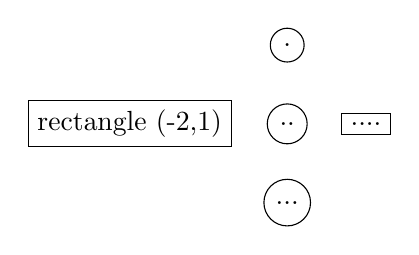
\begin{tikzpicture}
\path ( 0,2) node [shape=circle,draw] {.}
( 0,1) node [shape=circle,draw] {..}
( 0,0) node [shape=circle,draw] {...}
( 1,1) node [shape=rectangle,draw] {....}
(-2,1) node [shape=rectangle,draw] {rectangle (-2,1)};
\end{tikzpicture}
\end{teXXX}
\medskip

\begin{tikzpicture}
\path ( 0,2) node [shape=circle,draw] {1}
( 0,1) node [shape=circle,draw] {\textbf{10}}
( 0,0) node [shape=circle,draw] {\textbf{100}}
( 1,1) node [shape=circle,draw] {\textbf{1000}}
(-2,1) node [shape=circle,draw] {\textbf{10000}};
\end{tikzpicture}

In the above code, this text is empty (because of the
|empty {}|). So, why do we see anything at all at all the nodes? The answer is the draw option for the node operation: It
causes the |shape| around the text" to be drawn. If you have an empty |{}|, PGF still sees the empty space as a character and justs draws around it. The reason is than TikZ automatically adds some space around the text. The amount is set
using the option |inner sep|. So, to increase the size of the nodes. Modifying the example slightly we get.



\begin{tikzpicture}
\path ( 0,2) node [shape=circle,draw] {.}
( 0,1) node [shape=circle,draw] {..}
( 0,0) node [shape=circle,draw] {...}
( 1,1) node [shape=circle,draw] {....}
(-1,1) node [shape=circle,draw] {.....};
\end{tikzpicture}

As you can observe the size of the circle has been adjusted to fit the text that is enclosing it. 
Another way to simply add a node is using the |at| syntax:

\begin{texexample}{The node command}{}
\begin{tikzpicture}
\node at (0,0) [circle, draw] {\textbf{100}};
\node at (1,1) [diamond,draw] {\textbf{100}};
\end{tikzpicture}
\end{texexample}

The \cmd{\node} is an abbreviation of the |\path| node. This is a much shorter syntax than |\path| where one would need to add a lot of redundant move-tos  \seepgfmanual{215}.

If you have many nodes another way of achieving the example outlined above is to use the |\draw| command in comination with node and at.

\begin{texexample}{The node command}{}
\begin{tikzpicture}
\tikz \draw[fill=yellow!80!black]
(0,0) node {first node}
-- (1,1) node[draw, behind path] {second node}
-- (0,2) node[fill=red!20,draw,double,rounded corners] {third node};

\node at (0,0) [circle, draw] {\textbf{100}};
\node at (1,1) [diamond,draw]{\textbf{100}};
\end{tikzpicture}
\end{texexample}

\subsection*{Drawing shapes}

PGF abd \tikzname\ come with a number of predefined shapes:
\begin{itemize}
\item rectangle
\item circle, and
\item coordinate
\end{itemize}


\begin{tikzpicture}
\draw (0,0) circle (1cm);
\draw (0.5,0) circle (0.5cm);
\draw (0,0.5) circle (0.5cm);
\draw (-0.5,0) circle (0.5cm);
\draw (0,-0.5) circle (0.5cm);
\end{tikzpicture}



A circle is specified by providing its center point and the desired radius. The
command:

\medskip

\begin{tikzpicture}
  \draw[step=0.25cm,color=green] (-1,-1) grid (1,1);
  \draw (0,0) circle (1cm);
\end{tikzpicture}
\medskip

\begin{teXXX}
\begin{tikzpicture}
  \draw (x,y) circle (dia);
\end{tikzpicture}
\end{teXXX}



You  can use one |\draw| command to draw multiple circles as shown in \fref{fig:circles}


\begin{tikzpicture} 
 \draw (0,0) 
  circle (1cm)
  circle (0.6cm)
  circle (0.2cm)
 ;
\end{tikzpicture}

\emphasis{circle,begin,end}
\begin{teXXX}
\begin{tikzpicture} 
 \draw (0,0) 
  circle (1cm)
  circle (0.6cm)
  circle (0.2cm)
 ;
\end{tikzpicture}
\end{teXXX}





\begin{center}
\begin{tikzpicture}
\draw (0,0) circle (1cm)
circle (0.6cm)
circle (0.2cm);
\end{tikzpicture}
\captionof{figure}{You can use one draw command to draw multiple circles}
\label{fig:circles}
\end{center}
\captionof{figure}{Drawing multiple circles, using mutiple \texttt{circle} commands}


\subsection{Drawing ellipses}

Ellipses can be drawn in a similar fashion to circles. As an ellipse needs two center points to be specified the command used has the following general form:

\begin{verbatim}
\draw (a,b) ellipse (r1 dim and r2 dim);
\end{verbatim}

We can draw two ellipses as shown in the figure, using the code:
\begin{teX}
\begin{tikzpicture}[scale=0.6]
\draw[color=red] (0,0) ellipse (2cm and 1cm);
\draw[color=red] (0,0) ellipse (1cm and 2cm);
\end{tikzpicture}
\end{teX}

\begin{centering}
\begin{tikzpicture}[scale=0.6]
\draw[color=red] (0,0) ellipse (2cm and 1cm);
\draw[color=red] (0,0) ellipse (1cm and 2cm);
\end{tikzpicture}
\caption[Drawing ellipses]{Use the draw command in combination with ellipse to draw ellipses}
\end{centering}


\begin{teX}
\begin{tikzpicture}
\draw (0,0) ellipse (2cm and 1cm)
ellipse (0.5cm and 1 cm)
ellipse (0.5cm and 0.25cm);
\end{tikzpicture}
\caption{Drawing multiple circles, using mutiple \texttt{draw} commands}
\end{teX}

\section{Drawing more complicated shapes}
we can place a parabola in a rectangle as shown in \fref{fig:parabola}, by using the |rectangle| and the |parabola| options.

\bgroup
\centering

\begin{tikzpicture}
\draw[color=blue] (0,0) rectangle (1,1.5)
(0,0) parabola[color=orange] (1,1.5);
\draw[xshift=1.5cm] (0,0) rectangle (1,1.5)
(0,0) parabola[bend at end] (1,1.5);
\draw[xshift=3cm] (0,0) rectangle (1,1.5)
(0,0) parabola bend (.75,1.75) (1,1.5);
\end{tikzpicture}
\captionof{figure}{Parabolas drawn using the parabola and rectangle options.}
\label{fig:parabola}
\egroup




\emphasis{parabola,rectangle}
\begin{teX}
\begin{tikzpicture}
\draw[color=blue] (0,0) rectangle (1,1.5)
(0,0) parabola[color=orange] (1,1.5);
\draw[xshift=1.5cm] (0,0) rectangle (1,1.5)
(0,0) parabola[bend at end] (1,1.5);
\draw[xshift=3cm] (0,0) rectangle (1,1.5)
(0,0) parabola bend (.75,1.75) (1,1.5);
\end{tikzpicture}
\caption{Parabolas drawn using the parabola command}
\label{fig:parabola}
\end{teX}

\subsection*{The shape library}

\begin{tikzpicture}
\draw [help lines] (0,0) grid (2,2);
\draw [blue, dashed] (1,1) circle(1cm);
\draw [red, dashed] (1,1) circle(.5cm);
\node [star, star point height=.5cm, minimum size=2cm, draw]
at (1,1) {S};
\end{tikzpicture}

\section{Iterations}
One convenient construct provided with TikZ is a |foreach| command sequence

\begin{texexample}{Tikz loops}{tz:ex}
\centering
\begin{tikzpicture}[scale=2, color=bgsexy]
\foreach \i in {1,...,4}
{
  \path (\i,0) coordinate (X\i);
  \fill (X\i) circle (1pt);
}
  \foreach \j in {1,...,3}
{
  \path (\j,1) coordinate (Y\j);
  \fill (Y\j) circle (1pt);
}
\foreach \i in {1,...,4}
{
  \foreach \j in {1,...,3}
  {
     \draw[color=bgsexy] (X\i) -- (Y\j);
  }
}
\end{tikzpicture}
\captionof{figure}{Drawing a bi-partite garph using foreach loops}
\end{texexample}



\section{The pgfplots package}



\subsection{Loading data from files}

Scientific work, especially that associated with research tends to generate
a lot of data. The data would normally come from external applications and stored in files. With |TikZ| one can import the data
by using the word |file|:

\emphasis{addplot,file,x}
\begin{teXXX}
 \addplot file {./raw/wavefunctions/wavefunc\x.dat};
\end{teXXX}

In the example we use a file with a path. The data is saved in
files with the same name but a different ending. We use a |foreach| function to add the ending i.e, the file names are |wavefunc1|, |wavefunc2| and |wavefunc3|. By using external data files and the foreach command it can substantially reduce the amount of text in the macros. This improves debugging and readability.

\begin{texexample}[colback=white]{Loading files}{ex:lfiles}
\centering
\begin{tikzpicture}[scale=0.8]
    \begin{axis}[smooth,
    xlabel=$n$,
    ylabel=$\Theta{j}{n}$]
    \foreach \x in {0,...,2}
    {
        \addplot file {./raw/wavefunctions/wavefunc\x.dat};
    }
    \legend{$j=0$,$j=1$,$j=2$};
    \end{axis}
\end{tikzpicture}
\captionof{figure}{Example plot with data imported from external files, using \texttt{file}}
\end{texexample}


\begin{teXXX}
\begin{tikzpicture}[scale=0.6]
  \begin{axis}[
    xlabel=$n$,
    ylabel=$\Theta{j}{n}$]
    \foreach \x in {0,...,2}
    {
      \addplot file {./raw/wavefunctions/wavefunc\x.dat};
    }
    \legend{$j=0$,$j=1$,$j=2$};
  \end{axis}
\end{tikzpicture}
\end{teXXX}



\section*{Plotting functions}
Functions can be defined for plotting using a variety of methods. They are powerful but generally difficult to remember.



\section{Saving Data to a file}

You can save your data to a file in many ways. One easy way is to use
the \docpkg{filecontents} package. This package extends the LaTeX environment
with the same name, but allows you to overwrite the file {\protect\ctan{filecontents}}.

\begin{teXXX}
\documentclass[justified]{tufte-book}
\usepackage{pgfplots,lipsum,booktabs}
\usepackage{pgfplotstable}
\pgfplotsset{compat=newest}
\usepackage{filecontents*}
\begin{filecontents}{my1.dat}
    Label       value       num
    Integrity     33         4
    Standalone    14         3
    Interface      6         2
    Overall       18         1
\end{filecontents*}
\begin{document}
    your code here ...
\end{document}
\end{teXXX}

It is good practice to keep, such data at the top of your file, although with
the |filecontents| package, they can be inserted anywhere. Sometimes it maybe
easier to have a number of minimal files with the type of charts you using regularly and just update the data on top. In general if the data is entered
by hand rather than generated automatically by software this is a good way
to keep your work tidy.

\newenvironment{Chart}[1][black!70!green]{%
%%  defaults
    \gdef\level##1{Level ##1}
    \def\setchartwidth##1{%
      \def\chartwidth{##1}}%
    \setchartwidth{3.9cm}%
    \def\chartcolor{#1}
    \newcommand\addTitle[2][test]{
    
    
%% For the chart title we set it in a minipage for
%% better control
    \def\charttitle{\minipage{4cm}%
       \footnotesize %
       \centering\textbf{##2}\\##1%
       \endminipage}}%
   \def\xlabel{Completion (\%)}%
%% renders the chart 
    \def\renderChart{%
%%
    \footnotesize%
%%
%%
    \IfFileExists{#1.dat}{Test}{}
   \begin{tikzpicture}
   \begin{axis}[
    xbar, width=\chartwidth,title=\charttitle,
    y=0.5cm, enlarge y limits={true, abs value=0.75},
    xmin=0, xmax=100,enlarge x limits={upper, value=0.25},
    xlabel=\xlabel,
    %ylabel=Label,
    xmajorgrids=true,
    ytick=data,
    yticklabels from table={\dataTable}{Label},
    nodes near coords, nodes near coords align=horizontal
     ]
    \addplot[draw=none, fill=\chartcolor] table [x=value, y=num]
    {\dataTable};
    \end{axis}%
    \end{tikzpicture}}}
{}

\begin{comment}
\begin{figure*}
\centering

\hskip-2cm\begin{Chart}
 \addTitle[Mechanical Systems]{Shangri-la}
 \def\dataTable{SH-mechanical.dat}
 \renderChart
\end{Chart}\hspace{0.3cm}
\begin{Chart}
 \addTitle[FM-200 System]{All areas}
 \def\dataTable{my1.dat}
 \renderChart
\end{Chart}
\begin{Chart}
 \addTitle[Electrical Works]{Merweb}
 \def\dataTable{my6.dat}
 \renderChart
\end{Chart}
\caption{Mechanical Systems Shangrila. Commissioning status}
\end{figure*}


\begin{filecontents*}{my1.dat}
Label     value       num
Integrity         33            4
Standalone      14            3
Interface        6            2
Overall           18            1
\end{filecontents*}

\begin{filecontents*}{SH-mechanical.dat}
Label     value       num
{Fan coil units}       43             8
{Air Handling Units}       13             7 
{CW Pumps}       13             6
{ECU}       11             5
{Pressurization Fans}        15             4
{Smoke Extract Fan}       5             3
{Jet fan}       5             2
{Overall}       12              1
\end{filecontents*}

\begin{filecontents*}{my6.dat}
Label    value         num   other
{Level 7}  50           11   13
L6         90           10   12
L5       80             9    16
L4       90             8    18
L3       70             7    90
L2       80             6    21
L1       70             5    22
\end{filecontents*}

\begin{filecontents*}{carparkventilation.dat}
Label    value         num   other
L5         50           11   13
L4         90           10   12
L3         80           9    16
GR         90           8    18
B1         70           7    90
B2         80           6    21
B3         70           5    22
\end{filecontents*}
%% CO SYSTEM
%% DATA
\begin{filecontents*}{carparkco.dat}
Label    value         num   other
L5         78           7   13
L4         90           6   12
L3         80           5    16
GR         90           4    18
B1         70           3    90
B2         80           2    21
B3         70           1    22
B5         50          {}    {}
\end{filecontents*}

\begin{filecontents*}{carparkco2.dat}
value,   num,   other,
78,       7,   13,
90,       6,   12,
80,       5,    16,
90,       4,    18,
70,       3,    90,
80,       2,    21,
70,       1,    22,
\end{filecontents*}
\end{comment}






















%\let\luacmd\textbf
\chapter[Charts and Visualizations]{Presenting Data in Charts and Visualizations}
\label{ch:charts}
\pagestyle{headings}

There can be no doubt that the hallmark of scientific reports and publications is the graphical presentation of the results. Graphs show relationships underlying observations in a way no other device can provide\footnote{\textit{Doing science: design, analysis, and communication of scientific research}
 By Ivan Valiela}.  Charting is both an art and a science. Modern typography on charts and infographics look at Tufte as inspiration.
Tufte advocates to minimize the ink to data ratio and although this is not always possible it is good advice.
In this section we would look at charting in general which is probably of interest to most of the readers
in this book.  Another good source of information is Stephen Few’s website the \href{perpetualedge}{perceptualedge} \footnote{\protect\url{http:\\perceptualedge.com}}  with a number of excellent articles on data visualization. 



\captionsetup[figure]{name=Photo,parindent=0pt,minmargin=0pt,width=3sp,labelsep=period,skip=5pt,margin={0pt,0pt},margin*={0pt,0pt},position=bottom,singlelinecheck=on}

\begin{figure}[htbp]
\parindent=0pt
\centering

\includegraphics[width=0.8\linewidth]{./images/medieval-calendar.png}

\parindent-1em
\noindent\caption{This 1496 manuscript shows medieval calendars with depictions of the positions of the Sun and the Moon.}

\end{figure}

This chapter will focus more on charting rather than visualizations, as widely understood. These are best painted with a different tool. 

\begin{figure}[htbp]
\parindent=0pt


\includegraphics[width=\textwidth]{beautiful-evidence}

\caption{An extract from Tufte’s book \textit{Beautiful Evidence}. In his book Tufte advocates that science and art have in common \emph{intense seeing}, the wide-eyed observing that generates empirical information. \textit{Beautiful Evidence} is about how \emph{seeing} is turned into \emph{showing}. \cite{Tufte2006}}
\end{figure}

\section{Graphical Perception}

When a person looks at a graph, the information is decoded by the person’s visual system. A graphical method is successful only if the decoding is effective. Cleveland \cite{cleveland1985} in an often quoted study designed experiments and made suggestions as to how graphical data can be improved by selecting representations that have high rank in Table~ref{tbl:cleveland}. Cleveland and McGill at the time employed as statistical scientists at At \& T Bell Laboratories, investigated how we perceive quantitative information and produced a table as to how to order elementary tasks by accuracy. They suggested graphs should exploit tasks as high in the ordering as possible. The tasks are ordered from most accurate to least.


\begin{longtable}[c]{l>{\RaggedRight}p{7.5cm}}
\caption{Rank table for chart visual representation.}\label{tbl:ranktable} \\
\toprule
Rank  & Position along a common scale\\
\midrule
1  & Position along a common scale\\
2  & Position on identical but nonaligned scales\\
3  & Length\\
4  & Angle\\
    & Slope (with $\theta$ not too close to 0, $\pi/2$, or $\pi$ radians)\\
5   & Area\\
6   &Volume\\
     &Density\\
     &Colour saturation\\
7   & Colour hue\\         
\bottomrule
\end{longtable}





\begin{figure}[htbp]
\includegraphics[width=0.45\textwidth]{length-judgement}
\caption{The top panel is a divided bar chart. This graphical method requires length judgement; for example
to compare and order the values in group A is not easy. In the bottom panel the values are shown by a dot
chart. All values on the graph can be visually compared by judgements of position along a common scale, an
easier task. Now the ordering of the values in group A is easy to perceive. Adapted from \cite{cleveland1985}.}
\end{figure}

\section{How to Draw your Charts}

With the newer engines the limitations of fonts are now part of TeX’s history, so you can use other programs. However, the use of PGF and TikZ or pstricks is still an unbeatable way to produce high quality charts and graphs.
For visualizations other tools might be necessary. Asymptote is on of them and I am sure you have other in your toolbox.

\section{Tufte like charts}

During the last stages of a Project, it maybe easier to visualize the
main areas where effort needs to be exerted by using simple charts. One
such chart is shown in Figure~\ref{fig:tufte-overall}. When this chart
was prepared efforts were made to complete the physical installation
as well as plan and commission the plant. The use of colour in this
chart highlights the commissioning, so one can easily see the expectations. Although the percentages are written on top of the bars,
one need not read them to visualize how difficult is to achieve
100\% completion in a Project. On the other hand commissiong can go
fairly fast and can jump by a large percentage, just by
commissioning a couple of additional ELV systems that have approximately
a 10\% weigh factor.

One can easily fit approximately, six to seven months data on
a portrait chart, changing it around to landscape one can fit
more than a year. Personally I am not very happy with such long
projections as they are more like guesses rather than proper estimates.

One other chart that can be used to visualize progress and is more
commonly found in construction is the infamous S-curve. Now, if
the actual planning is detailed enough and granular enough to be
able to pin-point \textit{continuous} progress then it is
appropriate. using it if you can at least obtain weekly progress
estimates.


 
\begin{figure}[htbp]
\parindent0pt
\hspace*{-1.8cm}\begin{tikzpicture}
\footnotesize%

  \begin{axis}[
        ybar, axis on top,
        title={Cumulative Progress of Works},
        height=5cm, width=13.2cm,
        bar width=0.43cm,
        ymajorgrids, tick align=inside,
        major grid style={draw=white},
        enlarge y limits={value=.1,upper},
        ymin=0, ymax=100,
        axis x line*=bottom,
        axis y line*=left,
        y axis line style={opacity=0},
        ytick={0,25,50,75,100},
        tickwidth=0pt,
        legend style={
            at={(0.5,-0.2)},
            anchor=north,
            legend columns=-1,
            % adds space between the legends
            /tikz/every even column/.append style={column sep=0.7cm}
        },
        ylabel={Percentage (\%)},
        symbolic x coords={
           Sep-11,Oct-11,Nov-11,Dec-11,
           Jan-12,Feb-12,
           Mar-12,
           Apr-12},
       xtick=data,
       nodes near coords={
        \pgfmathprintnumber[precision=2]{\pgfplotspointmeta}
       }
    ]
    \addplot [draw=none, fill=gray] coordinates {
      (Oct-11, 98)
      (Nov-11,99)
      (Dec-11,99.5)
      (Jan-12,99.7)
      (Feb-12,99.8)
       };
   \addplot [draw=none,fill=gray!75!white] coordinates {
      (Oct-11, 96)
      (Nov-11,97)
      (Dec-11,98)
      (Jan-12,98.5)
      (Feb-12,99)
        };
   \addplot [draw=none, fill=gray!50!white] coordinates {
      (Oct-11, 50)
      (Nov-11, 60)
      (Dec-11, 70)
      (Jan-12, 80)
      (Feb-12, 90)
            };
    \addplot [draw=none, fill=orange!90!white] coordinates {
      (Oct-11, 25)
      (Nov-11, 35)
      (Dec-11, 45)
      (Jan-12, 55)
      (Feb-12, 65)
          };
    \legend{First Fix,Second Fix,Final Fix,Commissioning}
  \end{axis}
  \end{tikzpicture}\par
  
\captionsetup[figure]{name=Photo, labelsep=period,
                    skip=5pt, font=scriptsize,
                    position=bottom, margin{0pt,0pt}}
                    
\caption{Cumulative progress for all MEP works. Notice the slower rate of production during the last three months.}

\label{fig:tufte-overall}

\end{figure}


A good graph is uncluttered, clear and focused.

\subsection{Axis Lines}

Most problems with graphs arise from misuse of axes: too heavy, too long, wrong intersection,
ambiquous breaks or too confusing increments and incorrect proportions. An axis is a ruler that established
regular intervals for measuring the information provided. Axes may emphasize, diminish, distort, simplify
or clutter the information.

\clearpage

\begin{multicols}{2}
\subsection{Axis Length}

Graphs should utilize their space around them, as the graph itself is mostly white space. In publications the journal might want to minimize the cost of printing. An axis should not extend beyond the labeled unit od minor tick closest to the last data point.

\begin{tikzpicture}[scale=0.8]
\begin{axis}
\addplot coordinates {
(0,0)
(0.5,1)
(1,2)
};
\addplot coordinates {
(0,0)
(0.9,1.3)
(1.2,2.5)
};
\end{axis}
\end{tikzpicture}
\captionsetup[figure]{format=hang, name=Fig, font=footnotesize}
\captionof{figure}{Example Chart. This chart has no legend and also has no lables to indicate what the y-axis and x-axis represent.}
\label{fig:exchart}
\medskip


For example the chart shown in figure \ref{fig:exchart} has been typeset within a multicolumns environment and has utilized the space around it effectively. However it suffers from other short-comings. 

A figure, much like a table, has to be self-contained. No detail (symbol, line, etc.) of the figure should go undefined. In cases in which symbol
identifications are too long to be included in the data field, they are
included in the figure legend. Figure legends consist of figure numbers
and titles. The figure legend should briefly report what is in the graph,
not discuss the methods or meaning of the data. For reasons unknown
to me, it is customary for figure legends to be set below the graph;3
in contrast, you will recall that legends for tables are set on top of the
tables. \cite{ivan2001}

One should also consider the absence of axes, where they t represent.
\includegraphics[width=\linewidth]{math-tikz.pdf}
\end{multicols}


\section{The bullet graph}

The bullet graph is considered\footnote{\protect\url{http://www.perceptualedge.com/blog/?p=375}} to be a  better alternative to gauges in dashboards. A solution to a basic chart can be found at tx.se\footnote{\url{http://tex.stackexchange.com/questions/117314/is-there-any-package-to-create-bullet-gauge-graphs}}, by Jake, which sadly in a community of mathematicians, engineers and programmers was not popularized to the extend it deserved. 

Bullet gauges are commonly used to show the current state relative to a reference value with a background that divides the scale into regions.

\begin{figure}[htbp]
\centering

\includegraphics{./images/bullet-graph.png}
\caption{Bullet graph with annotations, indicating the various components of the graph.}
\end{figure}



current sales --
previous sales --
good -- 
great -- last shade box

Formatting: The color is preferable to be a range of distinct hues, which can also assist by those who are colorblind. It is also reproduced better when photocopies.  Intensities are preferred as follows:

three: 40\%, 25\% and 10\%

\makeatletter
\newenvironment {bulletgraph} {\luacode@begin\luacode@table@soft} {}
\makeatother

\pgfplotscreateplotcyclelist{bullet}{
{fill=color1, draw=none},
{fill=color2, draw=none},
{fill=color3, draw=none},
}

\pgfplotsset{mark options/.style={color=black!80}}
\pgfplotsset{barwidth/.style= {bar width=1.2ex} }
\pgfplotsset{chartheight/.style ={height=#1}}

\providecommand{\bulletgauge}[4][]{
    \begin{tikzpicture}[scale=0.8, font=\arial]
    \begin{axis}[
       width=8cm,
       chartheight = 60pt,
      % height=60pt,
       %y=2ex,
       xtick pos=left, 
       xtick = {0,50,...,400, 450},
       ytick=\empty,
       xmin=50, xmax=450,
        %enlarge y limits={abs=0ex},
        tick align=outside,
        axis on top,
        every axis title/.style={
            at={(rel axis cs:0,0.5)},
            anchor=east,
            align=right,
            xshift=-0.5em
        },
        #1
    ]
    \pgfplotsinvokeforeach{#4}{
        \pgfplotsset{cycle list name=bullet}
        \addplot +[xbar, bar width=7ex ] coordinates {(##1,0)};
    }
    \addplot [fill= barcolour, xbar, barwidth ] coordinates {(#2,0)};    
    \addplot [mark=|, mark options={very thick}, mark size=2ex, ] coordinates {(#3,0)}; 
    \end{axis}
    \end{tikzpicture}
}

\begin{scriptexample}{}{}
\begin{bulletgraph}
  m = require("i18n.bulletgraph")
 local data = {
     title = 'Valuation (Jan)',
     ranges = {230,300,500},
     bar = 200,
     marker = 220}
     local options = {
        barcolour = 'red!90'
   } 
m:render(data,options)        
\end{bulletgraph}
\medskip

\begin{bulletgraph}
   m = require("i18n.bulletgraph")
   local data = {
      title = 'Valuation (Apr)',
      ranges = {200,300,500},
      bar = 250,
      marker = 300}
   -- render the plot
   m:render(data,options)           
\end{bulletgraph}
\end{scriptexample}

Use an updated pgfplotsversion as we use |\pgfplotsset{compat=1.11}|, when we load the \pkgname{phd}. The environment |\begin{bulletgraph}|  is a |\luacode|  based environment and hence all the code has to be in lua syntax.

The code load the lua module |bulletgraph| and we the graph is rendered using the method \luacmd{render()}. The method, like most of the plotting routines provided by the package takes two arguments |data| and |options|.

\begin{texexample}{Bullet Plots}{ex:bulletplot}
\begin{bulletgraph}
local  bgraph = require("i18n.bulletgraph")
local data = {
     title = 'Valuation (Jan)',
     ranges = {230,300,500},
     bar = 200,
     marker = 220}
local options = {
        barcolour = 'red!90'
   } 
bgraph:render(data,options)        
\end{bulletgraph}
\end{texexample}

If you are familiar with Javascript you must have come across jQuery and its many plugins. The bulletgraph methods work in a similar fashion, where the options are a set of key values, that are used as a mixin with a set of default key values. If you only want to change the color of the bar, you only specify the color in the options the rest
are inherited from default values. All the \pkgname{phd} package routines, follow this design pattern to simplify the user interface and to enable typographical styles to be maintained throughout a publication. The best way to draw such charts is without the |options|. This separation of the interface, it also separates the data from the presentational aspects of drawing the plots.

\begin{texexample}{Bullet Plots (without options)}{ex:bulletplot1}
\begin{bulletgraph}
local  bgraph = require("i18n.bulletgraph")
local data = {
     title = 'Valuation (Jan)',
     ranges = {230,300,500},
     bar = 200,
     marker = 220}
bgraph:render(data,options)        
\end{bulletgraph}
\end{texexample}

\section{Using matplotlib}

Many researchers use Python to produce charts. A good guide can be found at \href{https://github.com/jbmouret/matplotlib_for_papers}{jbmournet} at github. There was also a good discussion at HN\footnote{\protect\url{https://news.ycombinator.com/item?id=9043571}}.












%\let\sidenote\footnote
\let\citep\footcite
\chapter{How to Develop your Own Class or Package}

\cxset {epigraph width=0.67\textwidth}

\epigraph{First there was one user and I took a lot of time to satisfy myself. Then I had 10 users, and a whole new level of difficulties arose. Then I had a hundred users and another level of things happened. I had a thousand users, I had ten thousand each of those were special phases in the development, important. I couldn't have gone with ten thousand until I'd done
it with a thousand. But each time a new wave of
changes came along, the idea was to have \tex get
better, and not get more diverse as it needed to handle
new things.}{Donald Knuth}

\parindent1em

\section{Introduction}


To \emph{make} a book is an interesting and somewhat involved process\footcite{town}. The text is set in type and printed on pages, the pages are gathered and folded into signatures and these are gathered and folded into signatures and these are then bound and covered. Many of the aspects of this process that has passed down to us by previous generations is discussed extensively in other sections of this book.  Class authors have to distill this knowledge in a set of typographical rules to be described in a class file. The first thing such an author must do is to describe the \emph{rationale} of developing such a class. The |octavo| \citep{octavo} class was developed to enable printing books in dimensions that follow traditional styles. The \citep{memoir}  class to offer a flexible system on which other classes could be based and so does \citep{koma}. The |tufte-book| and |tufte-handout| classes to provide a style that resembles those found in Tufte books. Many Universities offer \emph{Thesis} classes to standardize the way these are produced. Many of these Universities, translated the styles previously typed and the results are a typographical disaster, only mitigated by the ability to display beautiful mathematics. As these are printed on standard \emph{photocopy paper} one cannot do much with the layout. 

\section{Identifying your class}

The first thing a class must do is to identify any other formats it needs and to announce
its name. This is accomplished using the two commands 
\refCom{NeedsTeXFormat} and \refCom{ProvidesClass}.

The following example, delares the version of \LaTeXe\ that it requires and then
gives the class name. It can be found in the preable of most well written classes. You should also put some remarks to identify you as the author, the version number and other similar details. These are discussed in more detail in the next Chapter, where you will see how to automate documentation for your class.

\begin{teX}
\NeedsTeXFormat{LaTeX2e}[1994/06/01]
\ProvidesClass{myclass-book}[2010/12/11 v3.5.0 myclass-book]
\end{teX}

The above syntax must be followed exactly so that this information can be
used by \texttt{LoadClass} or \texttt{documentclass} (for classes) or \docAuxCommand{RequirePackage}
 or\cmd{usepackage} (for packages) to test that the release is not too old.
The whole of this $<release-info>$ information is displayed by \docAuxCommand{listfiles} and
should therefore not be too long.

\begin{teX}
% Load the common style elements
\input{myclass-common.def}
\end{teX}


Another command that can be used is \docAuxCommand{ProvidesFile}. 
This is similar to the two previous commands except that here the fullname,
including the extension, must be given. It is used for declaring any files other
than main class and package files.

This is useful, if you decide to have your main definitions in a separate file.

\section{Class Options}

Before we see in detail how to add options to a class, we need to review a package called
\pkgname{xkeyval}. Unless you are in the business of re-discovering wheels, this is an absolute must
for developing, readable and maintenable code and your class is to provide many options. 
\begin{teX}
\usepackage[textcolor=red,font=times]{mypack}
\end{teX}

Class options are best set by using booleans\cmd{newboolean}.

We first set a new boolean that we |name@myclass@afourpaper.| This is used using the package
\texttt{ifthen}\sidenote{The ifthen package was developed by 
David Carlisle, can be downloaded at \url{ http://www.ifi.uio.no/it/latex-links/ifthen.pdf }} 
Then we can |DecalareOptionX| and we set the boolean to default to true. If the user then types

myclass[a4paper]

The a4paper options will be set. This is a much better and concise way of defining options.
\cmd{newboolean}


\begin{teX}
\newboolean{@myclass@afourpaper}
\DeclareOptionX[myclass]<common>{a4paper}
  {
   \setboolean{@myclass@afourpaper}
   {true}
  }
\end{teX}
\medskip

Note that the command provide by \texttt{ifthen} \docAuxCommand{setboolean} takes true or false, as \#2, and sets \#1 accordingly. In the above code we set the option as true. 


It is much easier and most programmers use the \texttt{ifthen} package to check
for option booleans

\begin{teX}
\ifthenelse{\boolean{@myclass@afourpaper}}
  {\geometry{
        a4paper,
        left=24.8mm,
        top=27.4mm,
        headsep=2\baselineskip,
        textwidth=107mm,
        marginparsep=8.2mm,
        marginparwidth=49.4mm,
        textheight=49\baselineskip,
        headheight=\baselineskip
    }
  }
 {}
\end{teX}

\section{Set-up the font sizes}

LaTeX does not provide definitions of all the font-sizes. Unless you are
extending an existing class, this is one of the first tasks you need to 
do in your new class.

Normally class authors will define all the commonly defined size commands,
such as  \cmd{small}, \cmd{normalsize} and other similar commands.

In the example shown below, we first start by defining the \cmd{normalsize} font
size. In this book the \cmd{\normalsize}  is defined as 14pt. We also define the vertical
spaces that we need to have abovedisplay and belowdisplayskip. These are all very difficult to
remember and once you have something you are happy with, just copy from class to class
or even define a samll definition file to keep them all together.


{\fontfamily{phv}\selectfont Helvetica looks like this}
and {\fontencoding{OT1}\fontfamily{ppl} Palatino looks like this}.


 The user has access to a number of commands which change the size of
 the fount, relative to the `main' size used for the bulk of the text.


 These \cmd{size} commands issue a \cmd{@setfontsize}\index{Latex kernel!@setfontsize} 
 command.

\begin{teX}
  \@setfontsize\size\font-size{baselineskip} where:
\end{teX}



  \begin{description}
    \item {font-size} The absolute size of the fount to use from
        now on.
    \item{baselineskip} The normal value of \cmd{baselineskip}
        for the size of the fount selected. (The actual value will be
       % |\baselinestretch| * \meta{baselineskip}.)
    \end{description}

A number of commands, defined in the \LaTeX  kernel, shorten the
following  definitions and are used throughout. These are:

    \begin{center}
    \begin{tabular}{ll@{\qquad}ll@{\qquad}ll}
    \verb=\@vpt= & 5 & \verb=\@vipt= & 6 & \verb=\@viipt= & 7 \\
    \verb=\@viiipt= & 8 & \verb=\@ixpt= & 9 & \verb=\@xpt= & 10 \\
    \verb=\@xipt= & 10.95 & \verb=\@xiipt= & 12 & \verb=\@xivpt= & 14.4\\
    \ldots
    \end{tabular}
    \end{center}


\subsection{Setting up the normalsize}
 The user command to obtain the `main' size is \cmd{normalsize}. \LaTeX\
 uses \cmd{@normalsize} \index{Latex kernel!@normalsize} when referring to the main size and maintains this
 value even if \doccmd{normalsize} is redefined. The \doccmd{normalsize} macro also
  sets values for \cmd{abovedisplayskip}, \cmd{abovedisplayshortskip} and 
\cmd{belowdisplayshortskip}.



\begin{teXXX}
%%
% Set the font sizes and baselines to match Tufte's books
% normalsize
%%
\renewcommand\normalsize{%
   \@setfontsize\normalsize\@xpt{14}%
   \abovedisplayskip 10\p@ \@plus2\p@ \@minus5\p@
   \abovedisplayshortskip \z@ \@plus3\p@
   \belowdisplayshortskip 6\p@ \@plus3\p@ \@minus3\p@
   \belowdisplayskip \abovedisplayskip
   \let\@listi\@listI}

\normalbaselineskip=14pt
\normalsize
\end{teXXX}



\begin{minted}{latex}
\renewcommand\small{%
   \@setfontsize\small\@ixpt{12}%
   \abovedisplayskip 8.5\p@ \@plus3\p@ \@minus4\p@
   \abovedisplayshortskip \z@ \@plus2\p@
   \belowdisplayshortskip 4\p@ \@plus2\p@ \@minus2\p@
   \def\@listi{\leftmargin\leftmargini
               \topsep 4\p@ \@plus2\p@ \@minus2\p@
               \parsep 2\p@ \@plus\p@ \@minus\p@
               \itemsep \parsep}%
   \belowdisplayskip \abovedisplayskip
}
\renewcommand\footnotesize{%
   \@setfontsize\footnotesize\@viiipt{10}%
   \abovedisplayskip 6\p@ \@plus2\p@ \@minus4\p@
   \abovedisplayshortskip \z@ \@plus\p@
   \belowdisplayshortskip 3\p@ \@plus\p@ \@minus2\p@
   \def\@listi{\leftmargin\leftmargini
               \topsep 3\p@ \@plus\p@ \@minus\p@
               \parsep 2\p@ \@plus\p@ \@minus\p@
               \itemsep \parsep}%
   \belowdisplayskip \abovedisplayskip
}
\renewcommand\scriptsize{\@setfontsize\scriptsize\@viipt\@viiipt}
\renewcommand\tiny{\@setfontsize\tiny\@vpt\@vipt}
\renewcommand\large{\@setfontsize\large\@xipt{15}}
\renewcommand\Large{\@setfontsize\Large\@xiipt{16}}
\renewcommand\LARGE{\@setfontsize\LARGE\@xivpt{18}}
\renewcommand\huge{\@setfontsize\huge\@xxpt{30}}
\renewcommand\Huge{\@setfontsize\Huge{24}{36}}

%% Define a HUGE for fun
\newcommand\HUGE{\@setfontsize\Huge{38}{47}}  
\end{minted}


\section{Adjusting paragraph parameters}

 The parameters which control \TeX 's behaviour when typesetting
 paragraphs receive a bit of a tweak here. Contrary to the usual
 behaviour of modifying the grid with glue when difficulties are
 encountered with vertical space, here we shall try to counteract
 these tendencies and enforce as much as possible uniformity of the 
 grid of lines.

A good value for paragraph indentation is \texttt{parindent 0.5pt}, for vertical spacing between
paragraphs that are indented use 0pt. At this point if you are using any marginals it is a good idea
to allow hyphenation with the \docpkg{ragged2e} package. Since marginals use very narrow paragraphs you may
get a very funny looking marginal text. Using the package, adjustments can be made to hyphenate
the marginal text.

\begin{teXXX}
%%
% \RaggedRight allows hyphenation

\RequirePackage{ragged2e}
\setlength{\RaggedRightRightskip}{\z@ plus 0.08\hsize}
\setlength{\RaggedRightParindent}{1pc}

% Paragraph indentation and separation for normal text
\newcommand{\@tufte@reset@par}{%
  \setlength{\RaggedRightParindent}{1.0pc}%
  \setlength{\parindent}{1pc}%
  \setlength{\parskip}{0pt}%
}
\@tufte@reset@par

% Paragraph indentation and separation for marginal text
\newcommand{\@tufte@margin@par}{%
  \setlength{\RaggedRightParindent}{0.5pc}%
  \setlength{\parindent}{0.5pc}%
  \setlength{\parskip}{0pt}%
}
\end{teXXX}


\section{Formatting Chapters and Sections}

The section on Chapters etc, has more on this, but we will touch on it briefly.
Most recent class developerss use the \pkg{titlesec} and \pkg{titletoc} package to handle the complexity 
of these commands. With the |phd| package this is unecessary. 

\begin{teXXX}
\titleformat{\subsection}%
  [hang]% shape
  {\normalfont\large}% format applied to label+text removed \itshape
  {\thesubsection}% label
  {1em}% horizontal separation between label and title body
  {}% before the title body
  []% after the title body
\end{teXXX}

These are normally followed by the ``titlespacing" commands to define the space around these sections.

\begin{teXXX}
%% We set the titlespacing using the package titlesec and titletoc
%
\titlespacing*{\chapter}{0pt}{20pt}{40pt}
\titlespacing*{\section}{0pt}{3.5ex plus 1ex minus .2ex}{2.3ex plus .2ex}
\titlespacing*{\subsection}{0pt}{3.25ex plus 1ex minus .2ex}{1.5ex plus.2ex}
\end{teXXX}

\section{Adjusting the Index}

For classes representing books, the index is treated like a chapter whereas for others it is normally
treated like a section. Whatever your document ends up like, indices are best done in a multi-column environment.
One possibility is shown below, using the package "multcol".

\begin{teXXX}
\RequirePackage{multicol}
\renewenvironment{theindex}
  {\begin{fullwidth}%
    \small%
    \ifthenelse{\equal{\@tufte@class}{book}}%
      {\chapter{\indexname}}%
      {\section*{\indexname}}%
    \parskip0pt%
    \parindent0pt%
    \let\item\@idxitem%
    \begin{multicols}{3}%
  }
  {\end{multicols}%
    
\renewcommand\@idxitem{\par\hangindent 2em}
\renewcommand\subitem{\par\hangindent 3em\hspace*{1em}}
\renewcommand\subsubitem{
    \par\hangindent 4em\hspace*{2em}
}
\renewcommand\indexspace{
    \par\addvspace{
       1.0\baselineskip plus 0.5ex minus 0.2ex}\relax
    }%
%we now  swallow the letter heading in the index
\newcommand{\lettergroup}[1]{}

\end{teXXX}

The code, renews the "theindex" environment, with minor tweaks and defines it as a three column
layout at "fullwidth".

\section{Provide some hooks}
It is useful at the end of the class to allow for localization of the class
by importing a local file. This is easily achieved by checking if the file exists
and then loading it.  If there is a |myclass-book-local.sty|  file, load it.

\begin{teX}
\IfFileExists{myclass-book-local.tex}
  {input{myclass-book-local}
   \MyClassInfoNL{Loading myclass-book-local.tex}}
  {}
\end{teX}

If you intent to publish your class, you may also want to consider adding a hook for a patch-file.


\section{The final act of kindness to your users}
Many common classes, such as the |memoir| use such a tactic to avoid breaking old code.\index{IfFileExists}

\begin{teX}
 \IfFileExists{mypatch.sty}{%
 \RequirePackage{mypatch}}{}
\end{teX}


\parindent1em
\chapter{How to Package Your Class}

In the previous chapter we have outlined the main sections that you probably need
to define in your class. In the examples we have used we just typed the examples
as |example.cls| or |package.sty|.

In this chapter we will go over the packaging of the class
and automating the generation of user documentation, using the |doc| and \pkg{DocStrip}\footcite{docstrip}
programs in files with an extension |.dtx|. The DocStrip program is an amazing piece of code that was originally
created by Frank Mittelbach to accompany the |doc| package. The idea behind it was to remove comment lines
in order to reduce the execution time of the program. Having created the DocStrip program to remove comment lines from  programs it became feasible to do more than just strip comments.
Wouldn't it be nice to have a way to include parts of the code only when some
condition is set true? Wouldn't it be as nice to have the possibility to split the
source of a \tex program into several smaller files and combine them later into
one `executable'? Both these wishes have been implemented in the DocStrip program.



You should also be
familiar with ``LaTeX2e'' for Class and Package Writers”, which is available
from CTAN (\url{http://www.ctan.org}) and comes with most LaTeX2e" distributions
in a file called clsguide.dvi.\footcite{pakin2004}  Finally, you should know how to
install packages that are shipped as a \texttt{.dtx} file plus a \texttt{.ins} file.

style (.sty) file is primarily a collection of macro and
environment definitions. One or more style files (e.g., a main style file that
\cs{input}  or \cs{RequirePackages} multiple helper files) is called a package.
Packages are loaded into a document with \cs{usepackage}\marg{main .sty fille}.
In the rest of this document, we use the notation \meta{package} to represent
the name of your package.


Motivation The important parts of a package are the code, the documentation
of the code, and the user documentation. Using the \docpkg{Doc}  and
DocStrip programs, it’s possible to combine all three of these into a single,
documented LATEX(.dtx) file. The primary advantage of a .dtx file is that
it enables you to use arbitrary LATEX constructs to comment your code.
Hence, macros, environments, code stanzas, variables, and so forth can be
explained using tables, figures, mathematics, and font changes. Code can
be organized into sections using LATEX’s sectioning commands. Doc even
facilitates generating a unified index that indexes both macro definitions (in
the LATEX code) and macro descriptions (in the user documentation). 

This emphasis on writing verbose, nicely typeset comments for code—essentially
treating a program as a book that describes a set of algorithms—is known
as literate programming \cite{literate} and has been in use since the early days of \tex\ .

Furthermore,
this tutorial shows how to write a single file that serves as both documentation
and driver file, which is a more typical usage of the \texttt{Doc} system than
using separate files.

\subsection{The .ins file}

The first step in preparing a package for distribution is to write an installer
(|.ins|) file. An installer file extracts the code from a |.dtx| file, uses \pkg{docstrip}
to strip off the comments and documentation, and outputs a |.sty| file. The
good news is that a |.ins| file is typically fairly short and doesn’t change
significantly from one package to another.

\paragraph{License} The |ins| files usually start with comments specifying the copyright and license
information:

\begin{minted}{latex}
%%
%% Copyright (C) year by your name %%
%% This file may be distributed and/or modified under the
%% conditions of the LaTeX Project Public License, either
%% version 1.2 of this license or (at your option) any later
%% version. The latest version of this license is in:
%%
%% http://www.latex-project.org/lppl.txt
%%
%% and version 1.2 or later is part of all distributions of
%% LaTeX version 1999/12/01 or later.
%%
\end{minted}

The LATEX Project Public License (LPPL) is the license under which most
packages—and LATEX itself—are distributed. Of course, you can release your
package under any license you want; the LPPL is merely the most common
license for LATEX packages. The LPPL specifies that a user can do whatever
he wants with your package—including sell it and give you nothing in return.
The only restrictions are that he must give you credit for your work, and
he must change the name of the package if he modifies anything to avoid
versioning confusion.
The next step is to load DocStrip:

\begin{teXXX}
%%\input docstrip.tex
%%\keepsilent
\end{teXXX}



By default, DocStrip gives a line-by-line account of its activity. These messages
aren’t terribly useful, so most people turn them off, by using the command \docAuxCommand{keepsilent}:

\begin{teXXX}
\keepsilent
\end{teXXX}


A system administrator can specify the base directory under which all
TEX-related files should be installed, e.g., \texttt{/usr/share/texmf}. (See
\cmd{\BaseDirectory} in the DocStrip manual.) The |ins| file specifies where
its files should be installed relative to that. The following is typical:

\begin{teXXX}
\usedir{tex/latex/packagename}
\preamble
htexti \endpreamble
\end{teXXX}



The next step is to specify a preamble, which is a block of commentary that
will be written to the top of every generated file:

\begin{minted}{latex}
\preamble
----------------------------------------------------------------
phddoc --- A class to typeset LaTeX code.
E-mail: yannislaz@gmail.com
Released under the LaTeX Project Public License v1.3c or later
See http://www.latex-project.org/lppl.txt
----------------------------------------------------------------
\endpreamble
\end{minted}


The preceding preamble would cause |package.sty|  to begin as follows:

\begin{minted}{latex}
%%
%% This is file `phddoc.cls',
%% generated with the docstrip utility.
%%
%% The original source files were:
%%
%% phddoc.dtx  (with options: `class')
%% ----------------------------------------------------------------
%% phddoc --- A class to typeset LaTeX code.
%% E-mail: yannislaz@gmail.com
%% Released under the LaTeX Project Public License v1.3c or later
%% See http://www.latex-project.org/lppl.txt
%% ----------------------------------------------------------------
\end{minted}

We now reach the most important part of a .ins file: the specification of
what files to generate from the |.dtx| file. The following tells DocStrip to
generate hpackagei.sty from hpackagei.dtx by extracting only those parts
marked as `package'  in the .dtx file. (Marking parts of a .dtx file is
described later on.)

\begin{teXXX}
\generate{\file{<package>.sty}{\from{<package>.dtx}{package}}}
\end{teXXX}

\cmd{\generate} can extract any number of files from a given .dtx file. It can
even extract a single file from multiple |.dtx| files. See the DocStrip manual
for details.

Personally I also generate REDAME files in |markdown| format as well, so that
when they get uploaded to |github| they can be rendered nicely.

\begin{minted}{latex}
\generate{\file{\jobname.md}{\from{\jobname.dtx}{readmemd}}}
\end{minted}

The text has to be wriiten using `guards' with the tag |readmd|

\begin{minted}{latex}
%<*readmemd>
# The `phddoc` LaTeX2e class

The `phd` latex package and the class with the same name provide
convenient methods to create new styles for books, reports
and articles. It also loads the most commonly used packages 
and resolves conflicts.
%</readmemd>
\end{minted}

\subsection{Generating messages} 

The next part of a |.ins| file consists of commands to output a message to
the user, telling him what files need to be installed and reminding him how
to produce the user documentation. The following set of \cmd{Msg} commands is
typical:

\begin{minted}{latex}
\obeyspaces
\Msg{****************************************************}
\Msg{* *}
\Msg{* To finish the installation you have to move the *}
\Msg{* following file into a directory searched by TeX: *}
\Msg{* *}
\Msg{* packagei.sty *}
\Msg{* *}
\Msg{* To produce the documentation run the file *}
\Msg{* package.dtx through LaTeX. *}
\Msg{* *}
\Msg{* Happy TeXing! *}
\Msg{* *}
\Msg{****************************************************}
Note the use of \obeyspaces to inhibit \tex from collapsing multiple spaces
into one.
\endbatchfile
\end{minted}


Appendix A.1 lists a complete, skeleton .ins file. Appendix A.2 is similar
but contains slight modifications intended to produce a class (|.cls|) file
instead of a style (|.sty|) file

\section{The .dtx file}
We started describing the |.ins| install file first. The next file we will describe is
the |.dtx| file. This holds both the code definitions as well as the user documentation.

A |dtx|\ file contains both the commented source code and the user documentation
for the package. Running a |dtx|  file through |latex| typesets the
user documentation, which usually also includes a nicely typeset version of
the commented source code.

Due to some Doc trickery, a |dtx|  file is actually evaluated twice. The first
time, only a small piece of \latex\  driver code is evaluated. The second time,
comments in the |dtx|  file are evaluated, as if there were no `\%'  preceding
them. This can lead to a good deal of confusion when writing |dtx|  files
and occasionally leads to some awkward constructions. Fortunately, once
the basic structure of a |dtx|  file is in place, filling in the code is fairly
straightforward.

\paragraph{Guards} If you open any .dtx file you will notice that the lines either start with a \%
sign or sometimes with a percentage sign and |<guard>|. The latter is called a guard and they are in a way
like html tags. They have a starting and an ending tag. In the example below there are two different guards
|<*10pt>...</10pt>| and |<*11pt></11pt>|. Unlike html tags guards are boolean expressions! You can use:
\begin{quote}
\textbar  ! \&  
\end{quote}

The \textbar stands for disjunction (OR), the \& stands for conjunction (AND) and the ! (NOT) stands for
negation. The terminal is any sequence of letters and evaluates to true iff it
occurs in the list of options that have to be included.

\begin{minted}{latex}
%<*10pt|11pt|12pt>
... code
%</10pt|11pt|12pt>
\end{minted}

A longer example from KOMA shows the concept better.

\begin{minted}{latex}
%    \begin{macrocode}
\def\normalsize{%
%<*10pt>
  \@setfontsize\normalsize\@xpt\@xiipt
  \abovedisplayskip 10\p@ \@plus2\p@ \@minus5\p@
  \abovedisplayshortskip \z@ \@plus3\p@
  \belowdisplayshortskip 6\p@ \@plus3\p@ \@minus3\p@
%</10pt>
%<*11pt>
  \@setfontsize\normalsize\@xipt{13.6}%
  \abovedisplayskip 11\p@ \@plus3\p@ \@minus6\p@
  \abovedisplayshortskip \z@ \@plus3\p@
  \belowdisplayshortskip 6.5\p@ \@plus3.5\p@ \@minus3\p@
%</11pt>
... 
%    end{macrocode}
\end{minted}

If the guards only contain a one line of text, then a short form is provided as |<10pt>|. It is unecessary to provide a closing tag and the `*' is omitted. The example below from the KOMA classes shows a quite ingenious way of writing the |\ProvidesFile| macro in
the different files; one for each tag. 
Two kinds of optional code are supported: one can either have optional code
that `ts' on one line of text, like the example above, or one can have blocks of
optional code.
To distinguish both kinds of optional code the `guard modier' has been in-
troduced. The `guard modier' is one character that immediately follows the < of
the guard. It can be either * for the beginning of a block of code, or / for the end
of a block of code4. The beginning and ending guards for a block of code have to
be on a line by themselves.
When a block of code is not included, any guards that occur within that block
are not evaluated.


\begin{minted}{latex}
%    \begin{macrocode}
\ProvidesFile{%
%<10pt>  scrsize10pt.clo%
%<11pt>  scrsize11pt.clo%
%<12pt>  scrsize12pt.clo%
}[\KOMAScriptVersion\space font size class option %
%<10pt>  (10pt)%
%<11pt>  (11pt)%
%<12pt>  (12pt)%
]
%    \end{macrocode}
\end{minted}

In the |.ins| file one could write to generate the various |.clo| files.:

\begin{minted}{latex}
\generate{\usepreamble\defaultpreamble
  \file{scrsize10pt.clo}{%
    \from{scrkernel-version.dtx}{clo,10pt}%
    \from{scrkernel-fonts.dtx}{clo,10pt}%
    \from{scrkernel-paragraphs.dtx}{clo,10pt}%
  }%
  \file{scrsize11pt.clo}{%
    \from{scrkernel-version.dtx}{clo,11pt}%
    \from{scrkernel-fonts.dtx}{clo,11pt}%
    \from{scrkernel-paragraphs.dtx}{clo,11pt}%
  }%
  \file{scrsize12pt.clo}{%
    \from{scrkernel-version.dtx}{clo,12pt}%
    \from{scrkernel-fonts.dtx}{clo,12pt}%
    \from{scrkernel-paragraphs.dtx}{clo,12pt}%
  }%
}%
\end{minted}

\paragraph{The character table check } The second mechanism that Doc uses to ensure that a |dtx|  file is uncorrupted
is a character table. If you put the following command verbatim into
your |dtx|  file, then \pkg{Doc} will ensure that no unexpected character translation
took place in transport:

\begin{minted}{latex}
% \CharacterTable
% {Upper-case \A\B\C\D\E\F\G\H\I\J\K\L\M\N\O\P\Q\R\S\T\U\V\W\X\Y\Z
% Lower-case \a\b\c\d\e\f\g\h\i\j\k\l\m\n\o\p\q\r\s\t\u\v\w\x\y\z
% Digits \0\1\2\3\4\5\6\7\8\9
% Exclamation \! Double quote \" Hash (number) \#
% Dollar \$ Percent \% Ampersand \&
% Acute accent \’ Left paren \( Right paren \)
% Asterisk \* Plus \+ Comma \,
% Minus \- Point \. Solidus \/
% Colon \: Semicolon \; Less than \<
% Equals \= Greater than \> Question mark \?
% Commercial at \@ Left bracket \[ Backslash \\
% Right bracket \] Circumflex \^ Underscore \_
% Grave accent \‘ Left brace \{ Vertical bar \|
% Right brace \} Tilde \~}
A success message looks like this:
***************************
* Character table correct *
***************************

and an error message looks like this:
! Package doc Error: Character table corrupted.
\end{minted}

\paragraph{DoNotIndex} When producing an index, \pkg{doc} normally indexes every control sequence
(i.e., backslashed word or symbol) in the code. The problem with this level
of automation is that many control sequences are uninteresting from the
perspective of understanding the code. For example, a reader probably
doesn’t want to see every location where \cs{if} is used—or \cs{the} or \cs{let} or
\cs{begin} or any of numerous other control sequences.

As its name implies, the \cs{DoNotIndex} command gives |Doc| a list of control
sequences that should not be indexed. \cs{DoNotIndex} can be used any
number of times, and it accepts any number of control sequence names per
invocation:

\begin{teXXX}
\DoNotIndex{\#,\$,\%,\&,\@,\\,\{,\},\^,\_,\~,\ }
\DoNotIndex{\@ne}
\DoNotIndex{\advance,\begingroup,\catcode,\closein}
\DoNotIndex{\closeout,\day,\def,\edef,\else,\empty, \endgroup}
\end{teXXX}


\subsection{User documentation}

We can finally start writing the user documentation. A typical beginning
looks like this:

\begin{teXXX}
% \title{The \textsf{package} package\thanks{This document
% corresponds to \textsf{package}~\fileversion,
% dated~\filedate.}}
% \author{your name \\ \texttt{your e-mail address}}
%
% \maketitle
\end{teXXX}


The title can certainly be more creative, but note that it’s common for
package names to be typeset with \docAuxCommand{textsf} and for \docAuxCommand{thanks} to be used to
specify the package version and date. This yields one of the advantages
of literate programming: Whenever you change the package version (the
optional second argument to \docAuxCommand{ProvidesPackage}), the user documentation
is updated accordingly. Of course, you still have to ensure manually that
the user documentation accurately describes the updated package.

Write the user documentation as you would any \latexe document, except
that you have to precede each line with a |\%|. Note that the |ltxdoc| document
class is derived from article, so the top-level sectioning command is
|\section|, not |\chapter|.



\section{General tips for defining a Class}

Evaluate, if there is a class that is nearer to what you wish to achive. If not do a set of
requirements.

Book structure - start with book or |Octavo| if you need to hack extensively. If not use memoir, |koma| or |tufte-book|.

Paragraph looks

Lists

Figures

Bibliography and citations

Footnotes

Index

Titel pages

Book Cover

Language support

Mathematics

Graphs and figures

Typography - fonts, indentations fontsize etc

headers and footers


\section{Declaring Options}

Most classes or packages will have a good deal of options. These are declared using the
\docAuxCmd{DeclareOption} command. In this part no package loading should take place.

\begin{docCommand} {DeclareOption} { \marg{option} \marg{code}}
  The argument option is the name of the option being declared and the \marg{code} is the
  code that will execute if this option is requested.
\end{docCommand}


\begin{docCommand}{DeclareOption*} { \marg{code}}
  The argument \meta{code} in the star version of the command specifies the action to be 
  taken if an unknown option is specified. Within this argument the \docAuxCmd{CurrentOption}
  refers to the name of the option in question. 
  
\end{docCommand}

For example one could pass all such options
  to another package, using:
  \begin{verbatim}
  \DeclareOption*{\PassOptionsToPackage{\CurrentOption}{A}}
  \end{verbatim}


\section{Executing Options}

Normally after the options have been defined, one would need to provide default values and 
the options need to be executed. 

\begin{docCmd} {ExecuteOptions} { \marg{option list}}
  
\end{docCmd}

You can also |\ExecuteOptions| when declaring other options. There is one caveat. This command
can only be executed prior to executing the |\ProcessOptions| command because, as one of
its last actions, the latter command reclaims all of the memory taken up by the code for
the declared options.

\begin{docCmd} {ProcessOptions*} {}
\end{docCmd}

For some packages it is preferable or essential to process options in the order they
appear in the |usepackage| commands rather than using the order given through the
sequence of the \refCmd{DeclareOption} commands. In this case it one has to use
the star version of the command, i.e, |\ProcessOptions*| rather than |\ProcessOptions|.

\section{Special Commands for class files}

It is sometimes preferable to define a new class based on another and hence to extend it.
To support this concept the \latexe kernel provides two commands, \docAuxCmd{LoadClass} and
\docAuxCmd{PassOptionsToClass}. These two commands can then be used to develop a new class, by adding and extending the functionality of the loaded class.

\begin{docCommands}
\refCom{LoadClass}{ \oarg{option list}\marg{class}\oarg{release}}
\end{docCommands}  
  
For example the |ltxdoc| class loads the standard |article| class. The \pkg{tufte-book} class loads
the |book| class. The best way to understand the concepts discussed here is to
study these classes.

\section{A minimal class}

\begin{texexample}{Model Class}{ex:modelclass}

\begin{filecontents}{phdexampleclass.cls}
\NeedsTeXFormat{LaTeX2e}
\ProvidesClass{phdexampleclass}[2015/07/07]
\renewcommand\normalsize{\fontsize{}{10pt}{12pt}\selectfont}
\setlength\textwidth{6.5in}
\setlength\textheight{5in}
\pagenumbering{arabic}
\end{filecontents}

\end{texexample}






















%\newacro{SPQR}{Senatus Populusque Romanus}
\newacro{URL}{uniform resource locator}
\newacro{OUP}{Oxford University Press}

\chapter{Acronyms and Abbreviations}


In this section we will discuss the use and typesetting of symbols, abbreviations and acronyms. The |phd| package loads a number of packages and also offers a number of commands in managing symbols, abbreviations and acronyms. The main package we use to manage acronyms is \pkgname{acronym} \cite{acronym}. We also use some build-in commands for abbreviations and to assist in enforcing in-house style guides.  

\section{General Principles}

Abbreviations and symbols represent, through a variety of means, a
shortened form of a word or words. Abbreviations fall into three categories:
only the first of these is technically an abbreviation, though the
term loosely covers them all, and guidelines for their use overlap.

\begin{itemize}
\item \textit{Abbreviations} are formed by omitting the end of a word or words (VCR, lbw, Lieut.).
\item \textit{Contractions} are formed by omitting the middle of a word or words (I've,
mustn't, ne'er-do-well
\item \textit{Acronyms} are formed from the initial letters of words (SALT, Nazi, radar), the results being pronounced as words themselves.
\end{itemize}


\section{Acronyms}

An acronym is distinguished from other abbreviated forms by being a series of letters or 
syllables pronounced as a complete word: \textsc{NATO}
and UEFA are acronyms, but MI6 and BBC are not. Acronyms take no
points, whether all in caps (NAAFI, SALT, WASP), in initial capitals with
upper and lower case (Aga, Fiat, Sogat), or entirely in lower case (derv,
laser, scuba). Since they perform as words they can begin sentences, with
lower-case forms being capitalized normally, such as \textit{Laser treatment}. 

Any all-capital proper-name acronym is, in some house styles, fashioned
with a single initial capital if it exceeds four letters (Basic, Unesco, Unicef).

The \textit{Oxford Guide} suggests that editors should avoid this rule, useful though it is, where the result runs
against the common practice of a discipline (CARPE, SSHRCC, WYSIWYG), or where similar terms would be treated dissimilarly based on length alone.


Acronyms are not new language inventions, they were used well back in antiquity.  For example, the official name for the Roman Empire, and the Republic before it, was abbreviated as \ac{SPQR}. Inscriptions dating from antiquity, both on stone and on coins, use a lot of abbreviations and acronyms to save room and work. For example, Roman first names, of which there was only a small set, were almost always abbreviated. Common terms were abbreviated too, such as writing just "F" for "filius", meaning "son of", a very common part of memorial inscriptions mentioning people. Grammatical markers were abbreviated or left out entirely if they could be inferred from the rest of the text. \ac{SPQR}

So called \textit{Nomina Sacra} were used in many Greek biblical manuscripts. The common words "God" (Θεός), "Jesus" (Ιησούς), "Christ" (Χριστός), and some others, would be abbreviated by their first and last letters, marked with an overline. This was just one of many kinds of conventional scribal abbreviation, used to reduce the time-consuming workload of the scribe and save on valuable writing materials. The same convention is still commonly used in the inscriptions on religious icons and the stamps used to mark the eucharistic bread in eastern churches.

The early Christians in Rome, most of whom were Greek rather than Latin speakers, used the image of a fish as a symbol for Jesus in part because of an acronym—fish in Greek is ΙΧΘΥΣ (ichthys), which was said to stand for Ἰησοῦς Χριστός Θεοῦ Υἱός Σωτήρ (Iesous CHristos THeou hUios Soter: Jesus Christ, God's Son, Savior). Evidence of this interpretation dates from the 2nd and 3rd centuries and is preserved in the catacombs of Rome. And for centuries, the Church has used the inscription INRI over the crucifix, which stands for the Latin \textit{Iesus Nazarenus Rex Iudaeorum} (``Jesus the Nazarene, King of the Jews'').

The Hebrew language has a long history of formation of acronyms pronounced as words, stretching back many centuries. The Hebrew Bible ("Old Testament") is known as "Tanakh", an acronym composed from the Hebrew initial letters of its three major sections: Torah (five books of Moses), Nevi'im (prophets), and K'tuvim (writings). Many rabbinical figures from the Middle Ages onward are referred to in rabbinical literature by their pronounced acronyms, such as Rambam (aka Maimonides, from the initial letters of his full Hebrew name (Rabbi Moshe ben Maimon) and Rashi (Rabbi Shlomo Yitzkhaki).


The main package we load to assist with acronyms and abbreviations is |acronym|, developed by Tobias Oetiker \citeyearpar{acronym}. The package offers a number of useful commands to help with managing acronyms and to produce lists of acronyms and abbreviations. The package works by offering commands that you use to define an acronym as well as an environment serving the same purpose.

\begin{docCommand}{ac}{\meta{short version of the acronym}}
    To enter an acronym inside the text, use the |\ac{NATO}|
\end{docCommand}
    
    \begin{quote}
     |\ac{|\meta{acronym}|}|
    \end{quote}
    command. The first time you use an acronym, the full name of the
    acronym along with the acronym in brackets will be printed. If you
    specify the |footnote| option while loading the package, the full
    name of the acronym is printed as a footnote.
    The next time you access the acronym only the acronym will
    be printed.

\section{Symbols}

Symbols or signs, are a shorthand notation signifying a word or concept, and are frequent features of scientific and technical writing. The distinction between abbreviation and symbol may be blurred when, lie an abbreviation, a symbol is derived directly from a word or words (\textit{Ag} from \textit{argentum}, \textit{Pa} from \textit{pascal}, \textit{U} from \textit{uranium}), and in setting they are often treated similarly. Unlike abbreviations, however, symbols never take points, even if a single letter, or used alone or in conjuction with figures or words: \textit{F}  for \textit{false}, \textit{fluorine}, \textit{phenylalanine}.

Abstract, purely typographical symbols follow similar rules, being either close up (\ding{38}\ding{33}\ding{43})or spaced (\ding{38} \ding{33} \ding{43}). In \latex you can insert a non-breaking space if you want or a |hairsp|.

|\ding{38}~\ding{33}~\ding{43}|

Personally for the example I would prefer not to split them and the non-breaking space is a better option in this instance.

Symbols' uses can differ between disciplines. For example, in philological
works an asterisk (\textasteriskcentered) prefixed to a word signifies a reconstructed
form; in grammatical works it signifies an incorrect or nonstandard
form. A dagger (\textdagger) may signify an obsolete word, or 'deceased' when
placed before a person's name (this convention should be used only in
relation to Christians). In German a double dagger (\textdaggerdbl) follows the name
and signifies `killed in battle', \emph{gefallen} or  \gtrsymKilled.

A full set of these genealogical symbols can be found in the \pkgname{genealogytree} package  developed by  \person{Thomas F. Sturm} \citeyearpar{genealogytree} and are shown below,

\begin{scriptexample}[]{}{}
\textsl{\gtrSymbolsFullLegend[english]}
\end{scriptexample}

The package is loaded automatically by the |phd| package. Besides these symbols numerous other symbols
are loaded and described in the Chapter for Symbols.
\section{Abbreviations}

\subsection{Time Designations}

Most style guides recommend that you spell out the names of the months in the text but abbreviate them in the list  of works cited, except for May, June and July \cite{MLA}. The same manual suggests that words denoting units of time are also spelled out in the text (\textit{second}, \textit{minute}, \textit{week}, \textit{month}, \textit{year}, \textit{century}, some time designations are used only in the abbreviated form (\textit{a.m., p.m., AD, BC, BC, BCE, CE}). The |phd| package provides some assistance by loading the \pkg{datetime} package; more information on using it and of date and time formatting as well as calculations in Handling Dates and Time can be found in Pages~\pageref{ch:dates}--\pageref{datesend}.
\medskip

\begin{longtable}{lp{8cm}}
AD & after the birth of Christ (from the Latin \textit{anno Domini} `in the year of the Lord'; used before numerals ["\AD 14"] and after references for centuries ["twelfth century \AD"]\\
a.m. & before noon (from the Latin \textit{ante meridiem})\\
Apr. &April\\
Aug. &August\\
BC   &before Christ (used after numerals [``18 BC''] and referenced to centuries [``sixth century BC'']\\
BCE &before the common era (used after numerals and references to centuries)\\
CE  &common era (used after numerals and references to centuries)\\
cent. &century\\
Dec. &December\\
Feb  &February\\
Fri. &Friday\\
hr. &hour\\
Jan. &January\\
Mar. &March\\
min. &minute\\
mo. &month\\
Mon. &Monday\\
Nov. &November\\
Oct. &October\\
p.m. &after noon (from the Latin \textit{post meridiem})\\
Sat. &Saturday\\
sec. &second\\
Sept.&September\\
Sun. &Sunday\\
Thurs. &Thursday\\
Tues. &Tuesday\\
Wed. &Wednesday\\
wk. &week\\
yr. &year\\
\end{longtable}

Tables such as the one above, if not provided by the Publisher, can be very helpful, if you develop them on your own and refer back to them for consistency.

\subsection{Geographic Names}

\subsection{Common Scholarly Abbreviations and Reference Words}

\begin{figure}[tp]
\centering
\fbox{\includegraphics[width=1.0\textwidth]{./images/abbreviations.pdf}}
\caption{A typical Abbreviations page. This has been extracted from \protect\cite{bacchae}.}
\end{figure}


\section{The indefinite article with abbreviations}

The choice between \emph{a} and \emph{an} before an abbreviation depends on pronunciation,
not spelling. Use a before abbreviations beginning with a
consonant sound, including an aspirated h and a vowel pronounced with the sound of w or y.

\begin{scriptexample}
a BA degree a KLM flight a BBC announcer
a Herts, address a hilac demonstration a YMCA bed
a SEATO delegate a U-boat captain a UNICEF card
\end{scriptexample}

Use \emph{an} before abbreviations beginning with a vowel sound, including
unaspirated \emph{h}:

an AB degree an MCC ruling an FA cup match
an H-bomb an IOU an MP
an MA an RAC badge an SOS signal

This distinction assumes the reader will pronounce the sounds of the
letters, rather than the words they stand for (a Football Association cup
match, a hydrogen bomb). MS for manuscript is normally pronounced as
the full word, manuscript, and so takes a; MS for multiple sclerosis is
often pronounced em-ess, and so takes an. Likewise 'R.' for rabbi is
pronounced as rabbi ('a R. Shimon wrote'), but 'R' for a restricted classification
is normally pronounced as arr ('an R film').

The difference between sounding and spelling letters is equally important
when choosing the article for abbreviations that are acronyms and
for those that are not: a NASA launch but an NAMB award. The same holds
for names of symbols, which can vary: in America a hash symbol (\#) is a
'number sign' or, more formally, an \textit{octothorp}; in linguistic use an
asterisk may be called a 'star' and in mathematics an exclamation
mark called a 'factorial', 'shriek', or 'bang', so the correct forms are a *
and a ! rather than an * and an !. 

As abbreviated terms enter the
language there can be a period of confusion as to how they are pronounced:
in computing, for example, \ac{URL} is
pronounced by some as an abbreviation (you-are-ell) and others as an
acronym (earl), with the result that some write it as a URL and others as
an URL. Until a single pronunciation becomes generally accepted, the
best practice is simply to ensure consistency within a given work.

\section{Latin abbreviations}
\normalfont

Do not confuse 'e.g.' (\emph{exempli gratia}), meaning \enquote{for example}, with \enquote{i.e.}
{id est), meaning 'that is'. Compare hand tools, e.g. hammer and screwdriver
with hand tools, \ie those able to be held in the user's hands. Print both lower-case roman, with two points and no spaces, and preceded by a
comma. In OUP style 'e.g.' and 'i.e.' are not followed by commas, to avoid
double punctuation; commas are often used in US practice.

Although many people employ 'e.g.' and 'i.e.' quite naturally in speech
as well as writing, prefer 'for example' and 'that is' in running text.
(Since 'e.g.' and 'i.e.' are prone to overuse in text, this convention helps
to limit their profusion.) Conversely, adopt 'e.g.' and 'i.e.' within parentheses
or notes, since abbreviations are preferred there. A sentence in text cannot begin with 'e.g.' or 'i.e.'; however, a note can, in which case
they—exceptionally—remain lower case. The \textit{Oxford Guide} gives an example of exception to the rule

The package offers two commands:

\begin{verbatim}
\newcommand{\ie}{\textit{i.\hairsp{}e.}\xspace}
\newcommand{\eg}{\textit{e.\hairsp{}g.}\xspace}
\end{verbatim}

The commands handle the spacing and if they are to be in italics or not. Renew the commands to set the style you want.

\section{Units}
\label{units}

Most users of \latex will have a need for specifying units in  mathematical or text contexts. We load the \pkgname{siunitx} package. The package was developed by Joseph Wright\cite{siunitx}. The correct application of units of measurement is very important in technical applications. For this reason, carefully-crafted definitions of a coherent units system have been
laid down by the \textit{Conférence Générale des Poids} et Mesures (CGPM): this has resulted in
the \textit{Système International d’Unités} (SI). At the same time, typographic conventions for
correctly displaying both numbers and units exist to ensure that no loss of meaning
occurs in printed matter.

|siunitx| aims to provide a unified method for \latex users to typeset numbers and
units correctly and easily. The design philosophy of |siunitx| is to follow the agreed rules
by default, but to allow variation through option settings. In this way, users can use
|siunitx| to follow the requirements of publishers, co-authors, universities, etc. without needing to alter the input at all.



\begin{ddanger}
Angles can be typeset using the \cs{ang} command.  The
 \meta{angle} can be given either as a decimal number or as a
 semi-colon separated list of degrees, minutes and seconds, which
 is called \enquote{arc format} in this document. The numbers which
 make up an angle are processed using the same system as other numbers.
\end{ddanger}

%\parindent1em

\chapter{Boxes and glue in TeX}

\setlength{\columnsep}{2em}
{\it Once you understand \tex\rq{}s concept of glue, you may well decide that
it was misnamed; real glue doesn't stretch or shrink in such ways, nor does it
contribute much space between boxes that it welds together. Another word like
\emph{spring} would be much closer to the essential idea, since springs have a natural
width, and since different springs compress and expand at different rates
under tension. But whenever the author has suggested changing \tex's terminology,
numerous people have said that they like the word \emph{glue} in spite of its
inappropriateness; so the original name has stuck. }
\smallskip

{\hfill  ---  Donald E. Knuth}

\medskip   


\parindent1em




\newthought{Traditional typesetting} was a task that depended on assembling the types and inserting them one by one on holding frames. In a way it was an assembly of boxes.
The \tex typesetting system uses a similar model of boxes to typeset content but in addition it also uses the concept of glue to stretch or shrink the text so that it will look better typographically. Boxes contain
typeset objects, such as text, mathematical displays, and pictures, and glue
is flexible space that can stretch and/or shrink by amounts that are under
user control.

\begin{figure}[h]
\hbox{\drawfontbox{Qwerty}\drawfontbox{fjord}}
\caption{Everything is boxes.}
\end{figure}

\begin{center}
\printfontparams
\end{center}

\section*{Boxes}

Boxes in \tex have  a rectangular shape but have
three associated measurements called \emph{height}, \emph{width}, and \emph{depth}.
Figure \ref{fig:boxes} shows a 
picture of a typical box, showing its so-called \emph{reference point} and \emph{baseline}

The reason that they have three dimensions is that a character of text has normally three dimensions as shown in figure \ref{fig:boxes}. As characters need to be lined on a baseline, the depth provides a datum point on which they can be aligned and the depth provides a measure of the portion of the character that is below the baseline.


Boxes and glue are the main tools of \tex. The box can hold text and other items. Glue is simply spacing. It can be horizontal or veritcal spacing, and it can be made as rigid or as flexible as desired.



\textbf{One important feature of \tex is that it has no knowledge of the shape of the characters it typesets, just the dimensions of each character box.}


When \tex is typesetting, it is normally in horizontal mode, such as while
it is working on this paragraph. Otherwise, \tex can be in vertical mode, or
in math mode, or three others described in Chapter 13 of The \texbook.
Two low-level TEX commands for boxes are \cmd{hbox}, for a horizontal box,
and \cmd{vbox} for a box in vertical mode. In the latter, \tex is normally still
collecting material for display from right to left: it is not building up a
column of text, as in classical Chinese writing.

In both kinds of boxes, the result is an unbreakable object that acts
much like a single character. \tex reads input as a string of characters,
then breaks that string up in words, each of which forms a box. 
\emph{Word boxes}\index{word boxes}
are then collected into lines, lines into paragraphs, and paragraphs into a
page galley. The space between the words can be normal \emph{interword space},
or \emph{sentence-ending} space, which is somewhat larger in English-language
typesetting, and the space is normally glue, rather than of fixed size.

\tex has a sophisticated mathematical algorithm for figuring out the
best way to stretch or shrink interbox glue to optimize the appearance of
lines and paragraphs. Every so often, \tex checks to see whether it has
enough material saved on the growing page galley to fill a complete output
page, and it asynchronously (and effectively, unpredictably) calls the
output routine whose job it is to figure out where the page break should
happen, ship out a completed page to the |DVI|  file, and replace the galley by
whatever is left over.

In traditional \tex you  can force a line break with the carriage-return command \docAuxCommand{cr},
and a page break with the command \docAuxCommand{eject}, but \tex is an expert system,
and normally handles line and page breaking on its own. \latex provides its own commands such as \cmd{\clearpage} and \cmd{\newpage} and so do all other \tex based formats and systems.

\latex does not modify any of \tex's algorithms but simply it is a set of implemenation
macros.

\section{Units of measurement in TEX}

\tex allows you to specify sizes of typographical objects in any of nine different
units:


\begin{table}[htbp]
\begin{center}
\begin{tabular}{llp{5cm}}
\toprule
bp &big point &1 inch is exactly 72 bp; the PostScript pagedescription language uses these units, but just calls them points\\
cc &cicero: &1 cc is exactly 12 didot points, and is thus the European  analogue of the pica\\
cm &centimeter: &1 in is exactly 2.54 cm\\
dd &didot point: &1 dd is (1238/1157) pt, and is a typographical unit common in some parts of Europe\\
in &inch: &an archaic unit, roughly the width of a man's thumb; it has been discarded by most countries, but still used in the USA and its sattelites.\\
mm &millimeter: &1 in is exactly 25.4 mm\\
pc &pica: &1 pc is exactly 12 pt\\
pt &printer's point: &1 in is exactly 72.27 pt\\ 
sp &scaled point: &1 pt is exactly $2^{16}$ = 65536 sp.\\
\bottomrule
\end{tabular}
\end{center}
\end{table}



The units can be separated from their numeric value with optional space, so
\texttt{3pc} and \verb*+3 pc+ are equivalent. The little half box in the latter is a convenient
way to indicate explicit spaces in typewriter text. It can be printed by typing \cmd{\char32} and a suitable font or using |\textvisiblespace|.

Internally, \tex\ stores dimensions as integral numbers of scaled points:
1 sp is tiny ---  smaller than the wavelength of visible light.\footnote{The visible light has wavelengths from 380--450 nm for violet up to 620--750 nm for red (sp = 280 nm} It is sometimes
useful to create objects that small so that they differ from empty objects,
but are nevertheless invisible. It also ensures that TeX will look the same irrespective on which computer you actually compiled your document.

\tex deals only with 32-bit integer words, and does not take advantage
of extra precision available on historical machines with larger words. The
lower 16 bits of a dimension can be viewed as a fractional number of points,
and the uppermost bit is needed for a sign (0 for plus, 1 for minus). That
leaves 15 bits to hold an integral number of points, but TEX only expects 14
to be used, so that addition of two dimensions does not overflow. Thus, the
largest dimension in TEX is exactly 214 + (1 26) points, or about 5.758  
meters or 18.89 feet. 

\tex has several kinds of special storage locations, called registers, numbered
from 0 to 255. For example,\cs{dimen0} can hold a fixed dimension,
which can be specified in any of the nine units of measurement that are
recognized by \tex.

Here is how you can assign a dimension to a register, and then have \tex
display it back for you:

\begin{dispListing}
\dimen1 = 25.4mm (*@\protect\footnote{You shouldn't assign dimenensions to primitive registers, but rather use one of the allocation schemes provided by \latex to do so.}  @*)
\the\dimen1
\end{dispListing}


Notice that \tex’s output is always in points, showing that it converts different
input units to a common system of measurement.

You can convert a dimension to the much-smaller units of scaled points
by assigning it to another kind of \tex register designed to hold signed integers,
the\cs{count0} through\cs{count255} registers:

\begin{texexample}{}{}
\bgroup
  \dimen4 = 1pt
  \count4 = \dimen4
  \the\count4
\egroup
\end{texexample}

{\noindent This time we get the size as \texttt{sp} as 65536 }


You might have noticed that the conversion from inches to points was not
quite what we claimed in the summary of \tex units. Here is how to see the
differences:

\verb+\dimen1 = 1in+


\section{Skip registers}
\index{registers!skip}
\begin{docCommand}{skip}{}
\tex glue is specified as a fixed dimension, and optionally, with a plus and/
or minus dimension. Along with \cs{dimen} registers, TEX has glue registers,
called \cs{skip0} through \cs{skip255}. Here is how you can save glue settings in
 registers, and ask \tex to display the contents of one of them:
\end{docCommand}

\begin{texexample}{Skip counters}{ex:skipcounters}
\bgroup
  \skip1 = 10pt
  \skip2 = 10pt plus 3pt
  \skip3 = 10pt minus 2pt
  \skip4 = 10dd plus 3dd minus 2dd
  \the\skip4
  % 10.70007pt plus 3.21002pt minus 2.14001pt.
\egroup  
\end{texexample}


The four sample glue settings store, respectively, \textit{fixed glue}, \textit{stretchable
glue}, \textit{shrinkable glue}, and \textit{flexible glue} that can both stretch and shrink,
but only up to a specified amount. Interword and intersentence spaces are
generally defined with glue like this, so that if more stretch or shrink of
\index{glue}\index{glue!flexibe}\index{glue!stretchable}\index{glue!shrinkable}

\begin{teX}
\dimen2 = 72.27pt
\count1 = \dimen1
\count2 = \dimen2
\showthe \count1
> 4736286.
\showthe \count2
> 4736287.
\end{teX}

The two values differ by the tiny value 1 \textit{sp}, so we can in practice ignore
that difference. If we use higher-precision arithmetic, we find the exact
decimal equivalents of the fractions as

\begin{teX}
4 736 286=65 536 = 72.269 989 013 671 875;
4 736 287=65 536 = 72.270 004 272 460 937 5;
4 736 286.72=65 536 = 72.27
\end{teX}


Actually \tex uses that last relation as the definition of the conversion of
inches to scaled points, so that our assignment of 1 in to \verb+\dimen1+ has to
be rounded to the nearest integral number of scaled points. That is why
in the round-trip conversion from decimal to binary and back to decimal,
1 in became 72.26999 pt. \tex guarantees that its output decimal numbers
are always converted on input back to the original binary numbers from
whence they came. For more on the story of \tex’s I/O conversions, see [3].


Both \tex and \latex define a number of predefined dimensions and these are discussed in the relevant Chapters discussing the \latex kernel. For example you may come across the \docAuxCommand{jot}, which is defined by \latex as:

\begin{teX}
\newdimen\jot
\jot=3pt
\end{teX}

\begin{texexample}{jot}{ex:jot}
\bgroup
\parindent\jot
This is some sample text with a one |\jot| left indentation. Which is really too small to see in a paragraph.
\egroup
\end{texexample}

Defining |\parindent=jot| we can see that the indentation almost disappeared. This is obvious since |\jot| is used normally for maths.

Glue is the binder that lets \tex\ do its job. This chapter discusses some
preset forms of glue and their uses. Along with glue parameters there are a
number of special commands for inserting glue. The most interesting have
different degrees of infinity, namely |\hfil|, |\hfill|, |\hfilneg|, |\hss|,
and their vertical counterparts. 

Because of the special spacing requirements of mathematics, \tex\ defines
skips and spacing that are valid in mathematics mode only. Examples are the
are the special preset |mu| glues of |\thickmuskip|,
|\medmuskip|, |\thinmuskip|.
The |\newskip| and |\newmuskip| commands allocate skip (or really glue)
or muskip registers respectively for special uses. For example the specific
glues surrounding section heads are held in glue registers. 

It should be noted that the various |\...muskip| do not cause horizontal
spacing in math mode by themselves. They are used with |\mskip| to actually
cause the insertion of the glue.

These are all various forms of horizontal (or math) mode commands that insert
infinite quantities of glue. |\hfil|, |\hfill|, |\hfilneg|, and |\hss| insert
|plus 1fil|, |plus 1fill|, |minus 1fil|, and |plus 1fil minus 1fil|. 
The first two are {\it stretch} glues, the third is {\it shrink} glue and the
last is both. It
should be noted that when \tex\ tries to stretch or shrink glue values, they
vary according to their value. If there exists both |fil| and finite value
glue in a box or line, then all the stretch if it is |plus| glue 
or shrink if it is |minus| glue will be in
the section with the |fil| glue. If there is |fill| glue and either |fil| or
finite glue, then all the stretch or shrink will be in the |fill| sections.
Similarly with |filll| glue, which is not supplied in as readily usable form.
The difference in behaviour between |\hfil| and |\hss| is that |\hss| glue
will allow the contents of a box to spill outside without resulting in an
overfull box while |\hfil| will only fill or push contents to the edge of the
box. The major use for these glues are to center or to force stuff to either
edge of a box.  For instance this

\begin{texexample}{}{}
\def\aline{\vrule \hfil one \hfil two \hfil three 
         \hfill four \hfil five \hfil six 
         \hfill seven \hfil eight \hfil nine\vrule}

\aline

This is a preset |mu| glue. |\medmuskip = 4mu plus 2mu minus 4mu| for use
with |\mskip|. This is \hbox{\strut\vrule$\mskip\medmuskip$\vrule}.
\end{texexample}

So far we have been using in our examples the primitive \tex |\skip| to allocate
skip registers. This is dangerous, as they might have been defined elsewhere and our
definitions will overwrite them. Plain \tex and \latexe provide an allocation scheme
where this is done automatically. 

\begin{docCommand}{newskip}{}
The command \cs{newskip}\meta{skip name} assigns a new skip or glue register to
the name |\<skip name>|. 

Glue values may be assigned to it by |\<skip name> [=] <glue>|.
This assigns a new muskip or muglue register to the name |\<muskip name>|. Glue
values may be assigned to it by |\<muskip name> [=] <muglue>|.

This is a preset |mu| glue. |\thickmuskip = 5mu plus 5mu| for use
with |\mskip|. This is \hbox{\strut\vrule$\mskip\thickmuskip$\vrule}.

This is a preset |mu| glue. |\thinmuskip = 3mu| for use
with |\mskip|. This is \hbox{\strut\vrule$\mskip\thinmuskip$\vrule}
\end{docCommand}


\newskip\hides 
\hides= -1000pt% plus 1fill

atest atest

\hskip\hides atest

\hides= -1000pt  plus 1fill

atest atest

\hskip\hides atest

|\vfil \vfill|

|\vfilneg|

|\vss|

These are the vertical analogues to the infinite horizontal glues and act in
much the same manner. See the section on |\hfil ...|.
 



\normalsize



\section{Glue}

\tex joins the boxes it creates with some special mortar as Knuth writes, called glue. To understand how glue works we will
borrow a figure from the \tex Book.

\begin{figure}
  \centering
  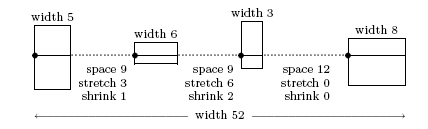
\includegraphics[width=0.9\linewidth]{./images/glue.png}
  \caption{Glue in \TeX}
  \label{fig:glue}
\end{figure}


\section{How to specify glue}

The usual way to specify \textit{glue} to \tex is
$<dimen>< plus~dimen><minus~dimen>$

where the plus and minus are optional and assumed to be zero if not
present; plus\index{glue!plus} introduces the amount of stretchability\index{glue!stretchability}, minus introduces the amount of shrinkability \index{glue!shrinkability}. 

For example, Appendix B of the TexBook defines \cs{medskip} to be an abbreviation for
|\vskip6pt plus2pt minus2p|. The normal-space component of glue must always be
given as an explicit dimen, even when it is zero. The ability of \TeX to stretch and shrink this glue has given it its beautiful looks. Strangely enough, although the algorithm is public it has not been used widely in other software.



\subsection{hfil and hfill}

{\obeylines
{This text will be flush left.\hfil}
{\hfil This text will be flush right.}
{\hfil This text will be centered.\hfil}
{Some text flush left\hfil and some flush right.}
{Alpha\hfil centered between Alpha and Omega\hfil Omega}
{Five\hfil words\hfil equally\hfil spaced\hfil out.}
}

Consider the following definitions:

\begin{verbatim}
\def\centerlinea#1{\hfil#1\hfill}
\def\centerlineb#1{\hfill#1\hfill}
\def\centerlinec#1{\hss#1\hss}
We define quickly a \cs{lineX}\footnote{Strange but my \LaTeX\ distribution has not got on. (This definition is from \texttt{plain.sty}}

\def\lineX{\hbox to\hsize}
\def\lineX{\hbox to\hsize}
\def\centerlinea#1{\hfil#1\hfil}
\def\centerlineb#1{\hfill#1\hfill}
\def\centerlinec#1{\hss#1\hss}

\lineX{\centerlinea{\test}}
\lineX{\centerlineb{\test}}
\lineX{\centerlinec{\test}}
\centerline{\test}
\begin{center}\test\end{center}

\end{verbatim}


\section{Specifying glue amounts}

\tex glue is specified as a fixed dimension, and optionally, with a plus and
or minus dimension. Along with \cs{dimen} registers, TEX has glue registers,
called \cs{skip0} through \cs{skip255}. Here is how you can save glue settings in
\tex registers, and ask \tex to display the contents of one of them:

\begin{teX}
\skip1 = 10pt
\skip2 = 10pt plus 3pt
\skip3 = 10pt minus 2pt
\skip4 = 10dd plus 3dd minus 2dd
\the \skip4
\end{teX}


\texttt{> 10.70007pt plus 3.21002pt minus 2.14001pt}

The four sample glue settings store, respectively, {\em fixed glue}, {\em  stretchable
glue}, {\em shrinkable glue}, and {\em flexible glue}  that can both stretch and shrink,
but only up to a specified amount. Interword and intersentence spaces are
generally defined with glue like this, so that if more stretch or shrink of  a
re underfull (too little text to fill the line), or overfull (too much text in the
line).



\section{Overfull lines}

Although overfull lines are reported in the \tex log file, they can be hard
to find in the typeset document if they only stick out a little. To make
them highly visible while you are fine tuning your final document, assign
the variable \cs{overfullrule} a nonzero dimension, such as 2 cm. \tex then
displays a solid black box, called a \emph{rule}, of that width in the right margin
on each line that is overfull. Using the \docpkg{microtype} package one can adjust the parameters to minimize this.

To make the rules disappear, simply remove it,
or comment out, the assignment, or reset its value to 0 pt. 

Just as you can assign dimension registers to count registers to convert
from points to scaled points, you can assign skip registers to dimension and
count registers to discard the flexible parts:


\begin{teX}
\skip1 = 10pt plus 3pt minus 2pt
\the\skip1
 \dimen1 = \skip1
\the \dimen1
\count1 = \skip1
\the \count1
\end{teX}




\section{More on glue in boxes}

Besides normal glue with fixed amounts of stretch and shrink, \tex also has
two kinds of glue that are \emph{infinitely} stretchable and shrinkable: \cs{hfil} and
\cs{hfill} in horizontal mode, and \cs{vfil} and \cs{vfill} in vertical mode. Notice that there two versions
of the commands, the one ends with one ell and the second one with two. The
two-ell forms are more flexible than the one-ell forms.

The boxes and glue model is powerful, and \tex's author, Donald Knuth,
has written that he views it as the key idea that he discovered when he
first sat down in 1977--1978 to design a computer program for typesetting.
For example, to set something flush left, put infinitely-stretchable glue on
its right. To set it flush right, put the glue on the left. For centered material,
put the glue on both sides. Here are four examples, with vertical
bars marking the ends of the horizontal box (boxes have no visible frames,
although it is possible to write \tex commands to give them such outlines,
and we use that feature shortly):





\section{Horizontal and vertical boxes}


\begin{docCommand}{hbox}{\marg{material}}
\end{docCommand}

Like their dimensions \TeX's boxes are not what one thinks when thinking of boxes. TeX's boxes come in basically two flavours, horizontal boxes and vertical boxes. An \cs{hbox} is created by the command \refCom{hbox}\marg{material}. It has the following properties:

\begin{enumerate}
\item The material is placed from left to right and it becomes a \textit{horizontal list}.\index{horizontal list}
\item The box \textbf{cannot be broken across lines}; it is an indivisible unit.
\end{enumerate}

An |hbox| can contain, characters, horizontal glue, horizontal leaders or other boxes. While in many cases these other boxes can be other |\hbox|es, |\vbox| can be used.


The \refCom{hbox} command has another form |\hbox to <dimen>|\marg{material}. This
creates a box whose width is the given (dimen). Thus |\hbox to lcm{<material>}|
will create a 1 inch wide box \hbox to 1cm{text}. However, we have to supply exactly 1 cm worth of
material to fill up the box; otherwise we end up with an error message. It is best
to consider this form of the command as a promise; we promise '\tex that we will
supply just enough material to fill up the box. 

We can place other hboxes in an hbox. By adding glue we can then move them left or right

\begin{texexample}{hbox and glue}{ex:hbox}
\bgroup
\Huge
\hbox to \textwidth{\hfill \hbox{\EOofficerI}\hbox{\EOofficerII}\hbox{\EOofficerIII} \hfill}

\hbox to \textwidth{\hfill \hbox{\EOofficerI}\hbox{\EOofficerII}\hbox{\EOofficerIII} \hfil}

\hbox to \textwidth{\hfill \hbox{\EOofficerI}\hfill \hbox{\EOofficerII}\hfill \hbox{\EOofficerIII} \hfill}
\egroup
\end{texexample}

The last command that affects the shape of an |\hbox| is 'spread(dimen)', which
spreads the box beyond its natural width. An |\hbox spread12pt|{(material)}
makes the box 12 points wider than its natural size. If the material in the box has
no flexibility, it cannot spread to fill up the additional space, resulting in an underfull
box. This is why 'spread' is normally used with flexible glues.

\begin{texexample}{hbox and glue}{ex:hbox}
\bgroup
\LARGE
\hbox to 5cm{\EOofficerI\EOofficerII\hfill\EOofficerIII}

\hbox spread5cm{\hfill\EOofficerI\hfill\EOofficerII\hfil\EOofficerIII}

\hbox spread9cm{\EOofficerI\hfill\EOofficerII\hfil\hfil\EOofficerIII}

\hbox spread7cm{\EOofficerI\hfill\EOofficerII\hfil\hfil\EOofficerIII} 


\makeatletter
\hb@xt@ 5cm {\EOofficerI\EOofficerII\hfill\EOofficerIII}
\makeatother
\egroup
\end{texexample}



Boxes can be moved up or down using |\raise| or |\lower|. Each of these primitives is followed by a dimension indicating how far the box can be lowered or raised.

Other material that can go in an hbox, is \textbf{vertical rules}. 

\subsection{The null macro}

The |\null| macro is defined both in Plain as well as LaTeX and generates an empty box. Its definition is:

\begin{teXXX}
\def\null{\hbox{}}
\end{teXXX}


\fbox{\hbox{This is a test}}

{
\fbox{\hsize=5cm
A test of a box at the end of a 2.0 inch line\par}

\fbox{\hsize=5.0cm in A test of a box at the end of a \hbox to 2cm{2.0 cm} line\par}

}

What happens when we have more than two boxes on a line? TeX will stuck them one under another. If they are enclosed within another hbox they will be inlined.



\begin{texexample}{}{}
\hbox to 1cm {A} \hbox to 1cm {B}

If we however, put them together in another |\hbox|, we get:

\hbox{\hbox to 1cm {A} \hbox to 1cm{B}}
\end{texexample}




An |\hbox| does not imply horizontal mode, so an attempt to start a paragraph with a box, for
instance
|\hbox to 0cm{\hss$\bullet$\hskip1em}Text ...|

will make the text following the box wind up one line below the box. It is necessary to switch
to horizontal mode explicitly, using for instance |\noindent| or |\leavevmode|. The latter is defined
using |\unhbox|, which is a horizontal command.


\begin{texexample}{}{}
\hbox to 0cm{\hss$\bullet$\hskip1em} Text ...


\leavevmode\hbox to 0cm{\hss$\bullet$\hskip1em} Text ...

\end{texexample}




\section{Kerning}


Using the command \cs{kern}, we can move boxes either left or right. Kerning is extensively used to build internal commands and we discuss it in more detail under the chapter for fonts.

\begin{docCommand}{kern}{\meta{dimen}}
A |\kern| is similar to glue [75], with two differences: (1) |\kern| is rigid; (2)
|\kern| specifies a point where a line, or a page, should not be broken. Since a box is
indivisible anyway, |\kern| is used in a box to indicate rigid spacing. It is interesting
to note that the same command, |\kern|, indicates horizontal spacing when used in
an |\hbox| and indicates vertical spacing when used in a |\vbox|.
\end{docCommand}
Consider two horizontal boxes, holding the letters A and V:
As you can observe, the letters AB are a bit afar, from what would be a visually pleasant arrangement, we can kern them as follows:
\medskip

\begin{teXXX}
\hbox{\Huge AV A\kern-5ptV}
\end{teXXX}
\medskip

Note that hbox, does not produce a frame. I~have used a frame |\fbox|, which will cover a bit later as well as scaled the image by 2, in order to see the effects more clearly.


\drawfontbox{\upshape\Huge FJord F\kern-5pt Jorp}





\noindent\begin{tabular}{ll}
|\hbox{\kern4pt A\kern8pt B\kern8pt C\kern4pt}| & \fbox{\hbox{\kern4pt A\kern8pt B\kern8pt C\kern4pt}} \\
~ &\\
\midrule
|\hbox{\kern4pt\raise1pt\hbox{A}|  & \fbox{\hbox{\kern4pt\raise1pt\hbox{A} \kern8pt BC\kern8pt\lower6pt\hbox{D} \kern4pt} \kern8pt BC\kern8pt\lower6pt\hbox{D}\kern4pt} \\
|\kern8pt BC|                      &\\
|\kern8pt\lower6pt\hbox{D}|        &\\
|\kern4pt}|                        &\\ 
|\kern8pt BC|                      &\\ 
|\kern8pt\lower6pt\hbox{D}|        &\\
|\kern4pt}| &\\
\midrule
\end{tabular}


\vbox{
\noindent\rule{\linewidth}{0.4pt}
\begin{minipage}{4.5cm}
 \begin{teXX}
\fbox{\hbox{\kern4pt A\kern8pt 
      B\kern8pt C\kern4pt}}
\end{teXX}
\end{minipage}
\hfill\hfill
\begin{minipage}{3cm}
\hfill\hfill\fbox{\hbox{\kern4pt A\kern8pt 
      B\kern8pt C\kern4pt}}
\end{minipage}

\medskip
\noindent\rule{\linewidth}{0.4pt}
}

Notice that an |\hbox| is constructed by setting its components side by side so that their \textit{baselines} are aligned. When \cs{raise}, \cs{lower} are used the baselines are no longer aligned. In such a case the baseline of the box is defined as the baseline shared by the components before any vertical movements. In the example above the box now has a depth, as a result of lowering |D|.


\vbox{
\noindent\rule{\linewidth}{0.4pt}
\begin{minipage}{4.5cm}
\begin{teXXX}
\hbox{\kern4pt\raise1pt\hbox{A} 
  \kern8pt BC\kern8pt
  \lower6pt\hbox{D} 
  \kern4pt} 
\end{teXXX}
\end{minipage}
\hfill
\begin{minipage}{3cm}
\fbox{\hbox{\kern4pt\raise1pt\hbox{A} 
\kern8pt BC\kern8pt\lower6pt\hbox{D} \kern4pt}}
\end{minipage}

\medskip
\noindent\rule{\linewidth}{0.4pt}
}



\noindent\textbf{Vertical boxes.}\quad A vertical box is build in a similar manner to that of a horizontal list, except it is composed of material in the \textit{vertical list}.
When horizontal boxes are added in the list, they are stuck on top of each other as shown in the example below. 
\medskip

\bgroup
\parindent0pt
\fbox{\vbox{\hsize=3cm\fbox{\hbox{ABCDEFGH}} \fbox{\hbox{AB}}}}
\egroup


\begin{docCommand}{vbox}{ to \meta{dimen}\marg{\meta{material}}}
Typesets a box in vertical mode.
\end{docCommand}

It is important to remember the two main differences between hboxes and vboxes. An hbox will expand to hold its material. If it need be it will overfill the line and produce an overful warning. A vbox will expand to hold its material. It is perfectly normal for a vbox to hold paragraphs, as shown. This is not possible with an hbox. However, the common pattern is for an |\hbox| to contain a |vbox| .

\begin{texexample}{hbox/vbox example}{ex:vbox}
\noindent\fbox{\vbox{\lorem\par\lorem\par}}

\hbox to \linewidth{\vbox{\lorem\par\lorem\par}}
\end{texexample}


\begin{docCommand}{hsize}{\meta{dimen}}
 Controls the width of text in a |vbox|.
\end{docCommand}

\noindent\textbf{Controlling the size of a vbox.}\quad What controls the size, is the containing environment. This in TeX, is specified using |\hsize|. In LaTeX this is controlled by an enclosing environment, maybe a minipage (which is build this way) or one of the page width parameters.


\begingroup
\parindent0pt
\fboxsep5pt
\hsize=3.9cm\footnotesize
\hfil\fbox{\vbox{\RaggedRight\lorem\par}} 
\hfil\fbox{\vbox{\RaggedRight\lorem\par}}
\hfil\fbox{\vbox{\RaggedRight\lorem\par}}\hfill
\endgroup
\captionof{figure}{Output to demonstrate the use of vboxes.}



The code to typest the boxes shown above follows:
\medskip
\emphasis{hsize}
\begin{teXXX}
\bgroup
\parindent0pt
\hsize=3.3cm\footnotesize
\hfil\fbox{\vbox{\lorem\par}} 
\hfil\fbox{\vbox{\lorem\par}}
\hfil\fbox{\vbox{\lorem\par}}
\hfill
\egroup
\end{teXXX}


Note, the use of \docAuxCommand{hsize}. We define the font size as |\footnotesize|. We have done this in order not to have overfull boxes--Latin words don't have a full set of hyphenation patterns in \latex. The macro |\lorem|, we have defined internally for this document. We place the code in a group in order not to affect the rest of the document.



\clearpage

\noindent\textbf{Vertical centering}\quad can be achieved by applying vertical infinite glue \cs{vfill}. In the example that follows, first we place two letters in individual |\hboxes| and we enclose them in a vbox. We apply |\vfill| both on top and at bottom.

\emphasis{\vfill}

\vbox{
\noindent\rule{\linewidth}{0.4pt}
\begin{minipage}{5cm}
\begin{teX}
\fbox{\vbox to 0.9cm{\vfil\hbox{M}\nointerlineskip\hbox{i}\vfil}} 
\end{teX}
\end{minipage}
\hfill
\begin{minipage}{3cm}
\hfill\fbox{\vbox to 0.9cm{\vfil\hbox{M}\nointerlineskip\hbox{i}\vfil}}\hfill\hfill 
\end{minipage}

\medskip
\noindent\rule{\linewidth}{0.4pt}
}



A |\vbox| can be combined with text and may appear anywhere within a paragraph. The baseline of the box will be aligned with the baseline of the current line.


\vbox{%
\noindent\rule{\linewidth}{0.4pt}}

\begin{teX}
A vbox can be placed within a paragraph \fbox{\vbox to 0.6cm{\vfil\hbox{M}\nointerlineskip\hbox{i}\vfil}} as shown here.


\hfill

A vbox can be placed within a paragraph \fbox{\vbox to 0.6cm{\vfil\hbox{M}
  \nointerlineskip\hbox{i}\vfil}} as shown here.

\end{teX}

\medskip
\noindent\rule{\linewidth}{0.4pt}






\noindent\textbf{Top alignment.}\quad\cs{vtop} is similar to a |\vbox|. The depth of this box is zero, since both A and B are capital letters. The width of this box is |\hsize|, since it contains text. 


\begin{codeexample}[]
\vtop{\hbox{A} \hbox{B}}
\end{codeexample}






Centering a picture in a box, both vertically and horizontally can be achieved using the methods we described so far.


\emphasis{hfill,hbox}
\begin{texexample}{}{}
     \fbox{%
          \vtop{\medskip
                    \hfill
                      \hbox{\includegraphics[width=1.5cm]{./images/amato.jpg}}%
                    \hfill 
                   \medskip%
                }%
      }%
\end{texexample}

\begin{texexample}{}{}
    \fbox{%
          \vtop{\medskip
                    \hfill
                      \hbox{\includegraphics[width=1.5cm]{./images/amato.jpg}}%
                      \hbox{\includegraphics[width=1.5cm]{./images/amato.jpg}}%
                      \hbox{\includegraphics[width=1.5cm]{./images/amato.jpg}}%    
                    \hfill 
                   \medskip%
                }%
      }%
\end{texexample}

Study the example a bit more carefully, as we have said earlier on that \cs{hbox}'es are stacked vertically, the reason why in the above example they are next to each other is that they are in an
\cs{fbox} which in turn is an \cs{hbox}  that can draw  frame around the box and is defined in the
\latex2e kernel.

So if we had only three images in hboxes we will get:

\begin{texexample}{Three Images Lined}{}
%\leavevmode
%\parindent30pt
\hbox{\includegraphics[width=1.5cm]{./images/amato.jpg}}%
\hbox{\includegraphics[width=1.5cm]{./images/amato.jpg}}%
\hbox{\includegraphics[width=1.5cm]{./images/amato.jpg}}%
\end{texexample}

An hbox does not start a paragraph. If we started a paragraph the behaviour will be different.

\begin{texexample}{Three Images Lined}{}
.\hbox{\includegraphics[width=1.5cm]{./images/amato.jpg}}%
\hbox{\includegraphics[width=1.5cm]{./images/amato.jpg}}%
\hbox{\includegraphics[width=1.5cm]{./images/amato.jpg}}%
\end{texexample}

If you notice carefully, we have started the paragraph by inserting a `.' before the first |\hbox|, an alternative way is to 
use |\leavevmode|. The effect of this command is to leave vertical mode, and to enter horizontal mode. Thus, if the mode is vmode (typically, outside any paragraph), a new paragraph is started. This paragraph may be flushed left, flushed right. 

\begin{texexample}{Three Images Lined}{}
\leavevmode
\hbox{\includegraphics[width=1.5cm]{./images/amato.jpg}}%
\hbox{\includegraphics[width=1.5cm]{./images/amato.jpg}}%
\hbox{\includegraphics[width=1.5cm]{./images/amato.jpg}}%

\meaning\leavevmode
\end{texexample}

The macro |\leavevmode| as its name implies forces \tex to leave vertical mode and enter horizontal mode. In this case the photos are just treated by \tex similarly to any character and tehy are typeset next to each other. 

\begin{docCommand}{kern}{}
If we wanted to add a bit of space between the horizontal images, we could use \cs{kern}
Kern again. This is from the book TeX for The Impatient page 157. You can use kern in math mode, but you cannot use the \texttt{mu} units. If you want to use \texttt{mu} units use \cs{mkern} instead.
\end{docCommand}

\emphasize{kern}
\begin{texexample}{}{}
\leavevmode
\hbox{\includegraphics[width=1.5cm]{./images/amato.jpg}}\kern10pt
\hbox{\includegraphics[width=1.5cm]{./images/amato.jpg}}\kern10pt
\hbox{\includegraphics[width=1.5cm]{./images/amato.jpg}}%
\end{texexample}

One needs to be careful as to where you issue |\leavevmode|. If it is in the middle of a paragraph it will have no effect.
\emphasize{This,is,some,text}
\begin{texexample}{Example with leavevmode}{}
This is some text
\leavevmode
\hbox{\includegraphics[width=1.5cm]{botticelli-34.jpg}}\kern10pt
\hbox{\includegraphics[width=1.5cm]{botticelli-34.jpg}}\kern10pt
\hbox{\includegraphics[width=1.5cm]{images/botticelli-34.jpg}}%
\end{texexample}

A very common way in \latex2e is to issue a |\par| command before |\leavevmode| to avoid this problem. Another way is to use
one of the |\ifvmode| or |\ifhmode| and act accordingly. We now fix our example and get what we want. 

\emphasize{par}
\begin{texexample}{}{}
This is some text
\par\leavevmode
\hbox{\includegraphics[width=1.5cm]{botticelli-34.jpg}}\kern10pt
\hbox{\includegraphics[width=1.5cm]{botticelli-34.jpg}}\kern10pt
\hbox{\includegraphics[width=1.5cm]{images/botticelli-34.jpg}}%
\end{texexample}

\begin{texexample}{}{}
   \HHUGE
   \fboxsep=0pt
   \fbox{%
          \vtop{\medskip
                    \hfill
                       \hbox{ H\kern10pt i\kern10pt j}%    
                       \hbox{ A\kern10pt C\kern10pt j}%
                    \hfill 
                   \medskip%
                }%
   }%
\end{texexample}

This example shows how letters are typeset and you can see that they are aligned at the baseline. They are no different than the eimage example that we have shown earlier, except we don't need the boxes.

\medskip

\vbox{
\noindent\rule{\linewidth}{0.4pt}
\begin{minipage}{4.9cm}
\begin{teX}
\centerline{$\Downarrow$}\kern 3pt%
\centerline{$\Longrightarrow$\kern 6pt% horizontal kern
  \textit{A note about kern}\kern 6pt
    $\Longleftarrow$}
\kern 3pt
\centerline{$\Uparrow$}  
\end{teX}
\end{minipage}
\hspace{0.3cm}
\begin{minipage}{4.5cm}
\centerline{$\Downarrow$}\kern 3pt%
\centerline{$\Longrightarrow$\kern 6pt% horizontal kern
  \textit{A note about kern}\kern 6pt
    $\Longleftarrow$}
\kern 3pt
\centerline{$\Uparrow$}
\end{minipage}

\medskip
\noindent\rule{\linewidth}{0.4pt}
}
\medskip

To make a point again, |\vbox| lines boxes at their bottom while, |\vtop| lines them at their top.

\medskip

\vbox{
\noindent\rule{\linewidth}{0.4pt}
\begin{minipage}{4.9cm}
\begin{teX}
 \hbox{\hsize=2cm \raggedright
\vbox to 0.5in{\hrule This box is .5in deep. \vfil\hrule}
\qquad
\vbox to 0.75in{\hrule This box is .75in deep. \vfil\hrule}
\qquad
\end{teX}
\end{minipage}
\hspace{0.3cm}
\begin{minipage}{4.5cm}
\hbox{\hsize=2cm \raggedright
\vbox to 0.5in{\hrule This box is .5in deep. \vfil\hrule}
\qquad
\vbox to 0.75in{\hrule This box is .75in deep. \vfil\hrule}
\qquad}
\end{minipage}

\medskip
\noindent\rule{\linewidth}{0.4pt}
}

\medskip


Trying the same with vtop

\medskip

\vbox{
\noindent\rule{\linewidth}{0.4pt}
\begin{minipage}{4.9cm}
\begin{teX}
 \hbox{\hsize=2cm \raggedright
\vbox to 0.5in{\hrule This box is .5in deep. \vfil\hrule}
\qquad
\vbox to 0.75in{\hrule This box is .75in deep. \vfil\hrule}
\qquad
\end{teX}
\end{minipage}
\hspace{0.3cm}
\begin{minipage}{4.5cm}
\hbox{\hsize=2cm \raggedright
\vtop to 0.5in{\hrule \smallskip This box is .5in deep. \vfil\hrule}
\qquad
\vtop to 0.75in{\hrule \smallskip This box is .75in deep. \vfil\hrule}
\qquad}

\hbox{\hsize=2cm \raggedright
\vbox to 0.5in{\hrule \smallskip This box is .5in deep. \vfil\hrule}
\qquad
\vbox to 0.75in{\hrule \smallskip This box is .75in deep. \vfil\hrule}
\qquad}
\end{minipage}

\medskip
\noindent\rule{\linewidth}{0.4pt}
}

\medskip

There are some other special macros defined by Plain TeX that we will only touch briefly here. One of them is \cs{underbar}{\index{Plain!\textbackslash underbar}.
The macro puts its argument into an hbox and underlines it.

\medskip

\vbox{
\noindent\rule{\linewidth}{0.4pt}
\begin{minipage}{4.9cm}
\begin{teX}
 \underbar{1,000,788.22}
\end{teX}
\end{minipage}
\hspace{0.4cm}
\begin{minipage}{4.0cm}
\medskip
\hfill\hfill{}\hspace*{1em}a1,000,700.22 \hfill

\smallskip

\hfill\[\underbar 1,000,788.22 \]\hfill
\end{minipage}

\medskip
\noindent\rule{\linewidth}{0.4pt}
}

\medskip


The \cs{everyvbox} command inserts a series of tokens at the beginning of every |\vbox|.


\medskip

\vbox{
\noindent\rule{\linewidth}{0.4pt}
\begin{minipage}{4.9cm}
\begin{teX}
 \everyvbox{$\bullet$}...
\end{teX}
\end{minipage}
\hspace{0.4cm}
\begin{minipage}{4.0cm}
\begingroup% Without this group, there are tons of problems!
   \everyvbox{$\bullet$}
   \global\setbox1=\vbox{This is a paragraph without an initial indent. It is   \the\hsize\ long lines.}
   \global\setbox2=\vtop{\copy1}
\endgroup
 \hbox{\box1} 

 \hbox{\box2}
\end{minipage}

\medskip
\noindent\rule{\linewidth}{0.4pt}
}

\medskip
Knuth in the TexBook Chapter 24, has some short description of the every commands. The `everyhbox` inserts a token list just before as its name implies a horizontal box.

Here is a short example. We define a `oneLineBox`, which is simply an hbox with some text and we add spread to spread the line. Using |\everybox| we add the letter \textbf{a} in each horizontal box. 


\tex considers the box overfull if the excess width of the box is larger than \cs{hfuzz} or \cs{hbadness} is less than 100. If I change  the badness to hbadness, I get 1000.

\medskip

\vbox{
\noindent\rule{\linewidth}{0.4pt}
\begin{minipage}{10.0cm}
\begin{teX}
 \begingroup
     \everyhbox{a}
     \def\oneLineBox#1#2%
     {%
          \hfuzz=0pt
          \overfullrule=0.25pt
          \setbox0=\hbox spread#2{#1}%
          \setbox1=\hbox{\the\badness}% 
          \setbox2=\hbox to 4.5cm{\box0\hfil\box1}%
          \box2
     }
     \oneLineBox{Badness of line }{-1em}
     \oneLineBox{Badness of line }{-0.54em}
     \oneLineBox{Badness of line }{-0.4em}
     \oneLineBox{Badness of line }{0em}
     \oneLineBox{Badness of line }{1em}
     \oneLineBox{Badness of line }{2em}
     \oneLineBox{Badness of line }{3em}
 \endgroup
\end{teX}
\end{minipage}


\begin{minipage}{10.0cm}
\begingroup
     \everyhbox{a}
     \def\oneLineBox#1#2%
     {%
          \hfuzz=0pt
          \overfullrule=0.25pt
          \setbox0=\hbox spread#2{#1}%
          \setbox1=\hbox{\the\badness}% 
          \setbox2=\hbox to 4.5cm{\box0\hfil\box1}%
          \box2
     }
     \oneLineBox{Badness of line }{-1em}
     \oneLineBox{Badness of line }{-0.54em}
     \oneLineBox{Badness of line }{-0.4em}
     \oneLineBox{Badness of line }{0em}
     \oneLineBox{Badness of line }{1em}
     \oneLineBox{Badness of line }{2em}
     \oneLineBox{Badness of line }{3em}
 \endgroup
\end{minipage}

\medskip
\noindent\rule{\linewidth}{0.4pt}
}

\medskip










\parindent1em




\section{More features of horizontal boxes}

Characters in the Latin alphabet have different shapes, and in most typefaces,
different widths. The letters \texttt{d f h k l t} have ascenders, making them
higher than the vowels \texttt{a e o u}, while the letters \texttt{f g j p q y} have descenders,
giving them added depth below the vowels. Similarly, an \texttt{m} is wider than
an \texttt{i}. 

\drawfontbox{(fjord)}

When \tex makes a normal horizontal box, the box width is the sum
of the widths of the characters, and the fixed parts of any glue, contained
in it. Shrink and stretch components of glue are discarded for the width
calculation. The box also has both a height above the baseline, the invisible
line on which the characters rest, and a depth below the baseline. The
depth is zero if there are no objects with descenders. The height and depth
are chosen from the largest vertical extents of the contained objects.

If you look carefully at typeset material, you will observe that, in most
typefaces, parentheses, brackets, and braces have both descenders and ascenders,
and the typeface designer usually makes their extents the maximum
among all of the characters in the design. This sample text shows
document: ( h g ) [ k j ] { l p }.

You can force TEX to choose a larger height and depth than normal when
you write a command for a horizontal box by ensuring that it has suitable
contents, such as an invisible vertical rule of zero width. The command

\verb+\hbox to 50pt {\vrule height 20pt depth 10pt width 0pt \it stuff}+

produces a box whose (invisible) outline looks like this: 

\hbox to 50pt {\vrule height 20pt depth 10pt width 0pt \it Great}

\drawfontbox{\kern 5pt\vrule height20pt depth 10pt width 1pt fjord}

The
three extents of the vertical rule can appear in any order, and any convenient
units.

In order to see the otherwise-invisible box edges in that example, we
used the \latex  built-in command \cs{fbox} to create a frame, and we eliminated
the default margin inside the frame by setting \cs{fboxsep = 0pt}. Plain \tex
does not have the \cs{fbox} command, but The TEXbook shows how to make
something like it on pp. 223 and 321.

One particular zero-width vertical rule is convenient for ensuring that
separate boxes all get the same height and depth. It has the height and
depth of parentheses in the normal prose font, and is given the macro name \refCom{strut}.
Its definition in the plain.tex file of macro definitions is roughly
equivalent to this:

\begin{docCommand}{strut}{}
\end{docCommand}

\begin{teX}
  \def \strut {\vrule height 8.5pt depth 3.5pt width 0pt}
\end{teX}

We insert a |\vrule| at the figure on the left below with a height of 20pt and a depth of 10pt. You can observe the difference on the right box, without the |\vrule|. The \textit{strut} is the blue line, which we gave a width of one point to make it visible. Real life struts, would have a width of 0pt and will not be visible. 

\drawfontbox{\kern5pt{\color{blue}\vrule height20pt depth 10pt width 1pt} fjord}
\drawfontbox{fjord}



\section{Horizontal alignment of boxes in TEX}
\fboxsep0.4pt

When horizontal boxes are set together, they are treated as separate words,
and therefore spaced accordingly. The input
\verb+ \fbox{one} \fbox{two} \fbox{three} \fbox{four}  +
produces  \fbox{one} \fbox{two} \fbox{three} \fbox{four}. As the example shows, we can put spaces
between them, or run them together so that they fit tightly.


\section{Vertical boxes in TEX}


\begin{minipage}{2.0in}
\begin{verbatim}
\noindent
\fbox{%
  \it
  \hbox to 80pt{%
     \parindent = 0pt
     \vbox to 30pt {%
         left text
         \vfil
         more left text%
     }%
  }%
}%
\end{verbatim}
\end{minipage}


%\noindent
\fbox{%
  \it
  \hbox to 80pt{%
     \parindent = 0pt
     \vbox to 30pt {%
         left text
         \vfil
         more left text%
     }%
  }%
}%

Firstly we use a noindent to ensure that the box is not indented. If you comment the\cs{fbox} out, you can see that the right amount of space has been left in the paragraph above.

\mbox{}
 
\noindent
\fbox{%
\it
\hbox to 80pt{%
\parindent = 0pt
\hsize = 80pt
\vbox to 30pt {\hfill right text
\vfil
\hfill more right text}
}%
}%



\noindent
\fbox{%
\it
\hbox to 80pt{%
\parindent = 0pt
\hsize = 80pt
\vbox to 30pt {\hfil center text
\vfil
 more center text \hfil}
}%
}%

We can aslo center the text for both lines, by modifying the code slightly.
\begin{teX}
\noindent
\fbox{%
\it \hbox to 80pt{
   \parindent = 0pt
   \hsize = 80pt
   \vbox to 30pt {
   center text \hfill
    \vfil
    \hfil more center text}
   }%
}%
\end{teX}


\noindent
\fbox{%
\it
\hbox to 80pt{%
\parindent = 0pt
\hsize = 80pt
\vbox to 30pt {\hfil center text
\vfil
\hfil more center text}
}%
}%



\chapter{Boxes with \protect\LaTeXe}

The \tex primitive commands have been abstracted by \latexe into more user friendly commands that are easier to use. One other reason for using these \LaTeX\ commands is that they are ``color safe''. Later on we will see other possibilities given by the \pkgname{color} or \pkgname{xcolor} package for drawing colored boxes, but we want to recall that the code for |\makebox| and the like has already a protection mechanism for colors, which the primitive commands do not have. \latexe also provides boxes that are self-aware of the width of their contents. For example |\fbox| will frame its contents in an |\hbox|. This simple task is very convoluted to achieve using basic \tex commands. 

\begin{docCommand}{framebox} {\marg{dim}}
One useful box command provided by \latex2e is \cmd{\framebox}. This command builds a box with any material you want to provide it with. The contents of this box are unbreakable, and as far as \tex is concerned it is treated the same way as it would treat a letter. 
\end{docCommand}

\begin{docCommand}{fboxsep}{\marg{dim}}
\end{docCommand}
\begin{docCommand}{fboxrule}{\marg{dim}}
Two associated lengths control the width of the rule and the space around the contents. We can change their default value by using |\setlength{\fboxsep}{0pt}| or just simply |\fboxsep=0pt| or even |\fboxsep0pt|. 
\end{docCommand}


Another interesting property is this: \emph{the contents of a box need not lie inside it}. You may have
noticed that, given the contents as an argument, the
|\framebox| command sets the dimensions of the box
to those of the contents (in reality, to the ``sub-boxes"
that compose the contents). But you can define the
dimensions explicitly as well. For example,

\begin{texexample}{framebox example}{ex:framebox}
|\framebox[13em]{Some text}|

\framebox[13em]{Some text}

\fcolorbox{theblue}{cyan}{Some text}

\end{texexample}

The box as is shown in the example will not break and it occupies more space than its contents. A second optional command allows us to typeset the contents, left, center or right.

\begin{codeexample}[vbox]
\fboxrule1pt

\framebox[13em][l]{Some text}\par

\framebox[13em][r]{Some text}\par

\framebox[13em][c]{Some text}\par

\framebox[1em][l]{Some text}\par

\framebox[1em][c]{Some text}\par

\framebox[1em][r]{Some text}\par
\end{codeexample}

As you can observe \latexe has abstracted the |\hfill| and similar commands and allows boxes to be constructed with ease. We have started the discussion with |\framebox|, but most practical uses of boxes is when they remain invisible.

\begin{docCommand}{makebox} { \oarg{width}\oarg{position}\marg{contents} } 
 is \latex's box workhorse.
 \end{docCommand}

The |source2e| manual states. If the width is missing, then position is also missing and |obj|  is put in an \cs{hbox} of its natural width. This is true as far as the looks are concerned, but not the behaviour, as you can see
from the following example is not an unqualified \cmd{\hbox} it is an hbox preceded by leavevmode.\footnote{\url{http://tex.stackexchange.com/questions/105585/latex2e-makebox-hbox}} This is of course good practice and brings consistency to the LaTeX kernel. I would recommend that you follow such practices in your own code. 

\begin{texexample}{}{}
\newbox\temp
\savebox\temp{test}
LaTeX

\makebox{test} \mbox{test}

TeX

\hbox{test} \hbox{test}

\indent\hbox{test} \hbox{test}

LaTeX with \cs{leavemode}

\makeatletter
\leavevmode\hbox to \wd\temp{test} \indent\hbox to \wd\temp{test}
\makeatother
\end{texexample}



\latex's analog of a\cs{hbox} is called \cs{mbox}. They are 
much the same thing, but \cs{mbox} is defined to be more widely usable. We have already used \latex's framed companion to \cs{mbox}, \cs{fbox}.

A horizontal box of specified width is provided in \latex with the command
\doccmd{makebox[width][position]\{contents\}}. Bracketed command arguments
in \latex are always optional. 

Here, the width is a \tex dimension,
and defaults to the natural width of the contents if not given. The position
is one of the letters \textbf{l} (flush left) or \textbf{r} (flush right); if it is omitted, the text
is centered in the box. If the specified width is smaller than needed, the
contents protrude from the box, and may overlap surrounding material. If
the specified width is zero, then we have equivalents of the TEX \cs{rlap} and
\cs{llap} commands.


Here are several examples of these three LATEX box commands:

{\obeylines
\mbox{stuff}

\fbox{stuff} 

|\makebox{stuff}|

|\makebox[40pt][l]{stuff}|

|\makebox[40pt][r]{stuff}|

|\makebox[0pt]{stuff}|

|\makebox[0pt][l]{stuff}|

|\makebox[0pt][r]{stuff}|
}



\subsection{Positioning boxes}

To help in positioning boxes within other objects, \latex provides the command
\docAuxCmd{raisebox} to raise and lower boxes:

\begin{teX}
\raisebox{raiselength}[height][depth]{contents}
\end{teX}

A negative first argument lowers the box, where the \cmd{\lowerbox} will lower the box. Here are some examples:

\begin{texexample}{Raising and lowering boxes}{ex:raise}
A \raisebox{10pt}{\fbox{upper}} A
upper
A \raisebox{10pt}{\
fbox{lower}} A
lower
A \fbox{\raisebox{10pt}[25pt]{\fbox{upper}}} A
upper
A \fbox{\raisebox{10pt}[
25pt]{\fbox{lower}}} A
lower
A \fbox{\raisebox{10pt}[25pt][15pt]{\fbox{upper}}} A
upper
A \fbox{\raisebox{10pt}[
25pt][15pt]{\fbox{lower}}} A
lower
\end{texexample}

\section{Paragraph Boxes}

\begin{docCommand}{parbox}{\oarg{position}\oarg{height}\oarg{innerpos}\marg{width}\marg{contents} }
  For longer strings of text, \latex provides the paragraph box \cs{parbox} 
\end{docCommand}


The optional position
is a letter \textbf{b} for alignment of the bottomline with the current baseline,
or \textbf{t} for alignment of the top line with the surrounding baseline. Without

The box can be used as if it were a letter or a word, so we can put it in
the middle of a sentence. The input

This is text \parbox{30pt}{\it and this is boxed text} and
this is more text.

This is text \fbox{\parbox{30pt}{\it and this is boxed text}}
and this is more text.
produces


Flush-right typesetting generally looks bad in narrow columns, so we
can insert a \cs{raggedright} command inside the last argument of the paragraph
box to get output like this:

\begin{texexample}{}{}

\parbox[b][120pt][t]{130pt}{\lorem}%
\hspace{1cm}%
\parbox[b][150pt][t]{130pt}{Only some short line of text here.}%



\parbox[b][120pt][t]{130pt}{\lorem}\hspace{1cm}\parbox[b][120pt][c]{130pt}{Only some short line of text here.}

\end{texexample}


\section{The minipage environment}

Another kind of paragraph box can be obtained in a more general, and
more powerful, way with the \docAuxEnv{minipage} environment:

\emphasis{minipage}
\begin{phdverbatim}
\begin{minipage}[position]{width}
   contents
\end{minipage}   
\end{phdverbatim}


The positioning works just like that for \verb+\parbox+, with alignment letters \textbf{b}
and \textbf{t}, and if they are omitted, a default of vertical centering.
In particular, verbatim text produced with the verb command is illegal
in macro arguments, so it cannot be used with \cs{fbox}, \cs{framebox}, \cs{makebox},
\cs{mbox}, or\cs{ parbox}, but it can be used inside a minipage. The input


\begin{texexample}{}{}
\begin{minipage}{170pt}
This is inline verbatim \verb=\verb|\%{}|=, and this
is a verbatim display:

\begin{verbatim}
#include <stdio.h>
#include <stdlib.h>
int main(void)
{
  printf("Hello, world\n");
  exit (EXIT_SUCCESS);
}
\end{verbatim}
\end{minipage}

\end{texexample}


A minipage can go everywhere and can hold virtually any content.


\section{Scaling and resizing boxes}

\begin{docCommand}{resizebox}{\marg{width}}{\marg{general material}}
Resizes the contents of a box
\end{docCommand}

The command \cs{resizebox}\marg{width}\marg{height}\marg{object} can be used with tabular to specify the height and width of a table. The following example shows how to resize a table to 8cm width while maintaining the original width/height ratio.

\begin{teX}
\resizebox{8cm}{!} {
  \begin{tabular}...
  \end{tabular}
}
\end{teX}

Alternatively you can use \cs{scalebox}{ratio}{object} in the same way but with ratios rather than fixed sizes:

\begin{teX}
\scalebox{0.7}{
  \begin{tabular}...
  \end{tabular}
}
\end{teX}

Both |\resizebox| and |\scalebox| require the \pkg{graphicx}\footfullcite{graphicx} package.
To tweak the space between columns (LaTeX will by default chose very tight columns), one can alter the column separation: |\setlength{\tabcolsep}{5pt}|. The default value is |6pt|.

The scalebox is great if you want to magnify a letter so that you can observe the design closer.

\bigskip
\noindent\begin{tabular}{|c|c|c|c|c|c|}\hline
Kp-Fonts & Kp-\textit{light} & CM & Palatino & Utopia & Times\\\hline\hline
\scalebox{2}{ag713} &
\scalebox{2}{\fontfamily{jkpl}\selectfont 7} &
\scalebox{2}{\fontfamily{lmr}\selectfont 713}  &
\scalebox{2}{\fontfamily{ppl}\selectfont 713}  &
\scalebox{2}{\fontfamily{put}\selectfont 7} &
\scalebox{2}{\fontfamily{ptm}\selectfont \oldstylenums{7}} \\\hline
\end{tabular}


\begin{teX}
\hspace{-6mm}\begin{tabular}{|c|c|c|c|c|c|}\hline
Kp-Fonts & Kp-\textit{light} & CM & Palatino & Utopia & Times\\
\hline\hline
  \scalebox{10}{a} &
  \scalebox{10}{\fontfamily{jkpl}\selectfont a} &
  \scalebox{10}{\fontfamily{lmr}\selectfont a}  &
  \scalebox{10}{\fontfamily{ppl}\selectfont 7}  &
  \scalebox{9.2}{\rule{0pt}{1.25ex}\fontfamily{put}\selectfont a} &
  \scalebox{10}{\fontfamily{ptm}\selectfont a}\\\hline
\end{tabular}
\end{teX}
\bigskip



\section{Glues with Negative and zero dimensions}

A box with a natural size of zero with the right glue amount can become very useful. For example the glue
|0pt plus1fil minus1fil| can stretch to infinity and also shring to minus infinity. Of course in the case of
\tex infinity is \docAuxCommand{maxdimen}. A \tex primitive is defined with this glue \refCom{hss}.

\begin{docCommand}{hss}{}
\end{docCommand}

There is also a corresponding \refCom{vss}.

\begin{docCommand}{vss}{}
\end{docCommand}


These macros place text on a full line either centred or left or right adjusted.

\begin{texexample}{}{}
\makeatletter
368 \def\@@line{\hb@xt@\hsize}
369 \def\leftline#1{\@@line{#1\hss}}
370 \def\rightline#1{\@@line{\hss#1}}
371 \def\centerline#1{\@@line{\hss#1\hss}}
\rlap
\llap
These macros place text to the left or right of the current reference point without
taking up space.
372 \def\rlap#1{\hb@xt@\z@{#1\hss}}
373 \def\llap#1{\hb@xt@\z@{\hss#1}}

$a\mathrel{\rlap{\;/}{=}}b $

{\Huge
\leavevmode
\rlap{Y}L
\rlap{C}\kern2.6pt\lower3.5pt\hbox{,}
}
\makeatother
\end{texexample}

\begin{docCommand}{rlap}{\marg{material}}

\end{docCommand}

Of course neither |llap| or |rlap| start a paragraph, so we need to use a |leavevmode| or one of the other ways to start a paragraph.

\begin{docCommand}{llap}{\marg{material}}
\end{docCommand}


\begin{docCommand}{smash}{\marg{material}}
The |\smash| command typesets the material with a height and depth of zero.
\end{docCommand}

\begin{docCommand}{phantom}{\meta{material}}
\end{docCommand}

\begin{docCommand}{vphantom}{\meta{material}}
\end{docCommand}

\begin{texexample}{Defining smash}{}
\bgroup
\def\smash{%
   \relax % \relax, in case this comes first in \halign
   \ifmmode
   \expandafter\mathpalette\expandafter\mathsm@sh
   \else
    \expandafter\makesm@sh
   \fi}
   
\def\makesm@sh#1{%
   \setbox\z@\hbox{\color@begingroup#1\color@endgroup}\finsm@sh}

\def\mathsm@sh#1#2{%
   \setbox\z@\hbox{$\m@th#1{#2}$}\finsm@sh}

\def\finsm@sh{\ht\z@\z@ \dp\z@\z@ \box\z@}
\egroup

\vbox{\smash {\hbox{A} } \hbox{B}} Test

\end{texexample}

\cxset{geometry units = pt,
       fontbox font=\Huge\upshape}

  


Consider the letters `Q' and `P', shown below. The capital letter `Q' has a depth of 1.72mm, we might wish to smash
it in a two line title block to reduce the line spacing between two consecutive lines. This can be accomplished with the
\refCom{smash} command.

\centerline{\drawfontbox{Q} \drawfontbox{P}}

Smashing it produces the following results.

\centerline{\drawfontbox{\vbox{\smash {\hbox{Q} } \hbox{P}}}  \drawfontbox{\vbox{\hbox{Q}  \hbox{P}}}}  

The command is more useful in math environments and is used extensively both by authors and package developers.

\begin{teXXX}
\def\rightarrowfill{$\m@th\smash-\mkern-7mu%
454 \cleaders\hbox{$\mkern-2mu\smash-\mkern-2mu$}\hfill
455 \mkern-7mu\mathord\rightarrow$}

456 \def\leftarrowfill{$\m@th\mathord\leftarrow\mkern-7mu%
457 \cleaders\hbox{$\mkern-2mu\smash-\mkern-2mu$}\hfill
458 \mkern-7mu\smash-$}
\end{teXXX}

Two further macros can be useful to authors of mathematical documents, \docAuxCommand*{phantom} and \docAuxCommand*{vphantom}. 

When typesetting roots, sometimes there are issues with heights. The following example
from \citetitle{mathmode}\footcite{mathmode} illustrates the point.

\begin{equation}
 \sqrt{a}\,%
 \sqrt{T}\,%
 \sqrt{2\alpha k_{B_1}T^i}\label{eq:root1}
\end{equation}

This can be corrected using \refCom{vphantom}. 

\begin{texexample}{Correcting height issues}{ex:sqrtheights}
\begin{equation}\label{eq:root2}
 \sqrt{a\vphantom{k_{B_1}T^i}}\,%
 \sqrt{T\vphantom{k_{B_1}T^i}}\,%
 \sqrt{2\alpha k_{B_1}T^i}
\end{equation}

\begin{equation}
x = \sqrt[3]{6+\sqrt[3]{6+\sqrt[3]{6+\sqrt[3]{6+\cdots}}}}
\end{equation}
\end{texexample}

Using \pkgname{amsmath} \docAuxCommand{smash} can be used for even better results when
using inline or displayed roots. It must be noted that \cs{smash} in \latexe is defined
without such an optional argument.



\makeatletter
\renewcommand{\smash}[1][tb]{%
\def\mb@t{\ht}\def\mb@b{\dp}\def\mb@tb{\ht\z@\z@\dp}%
\edef\finsm@sh{\csname mb@#1\endcsname\z@\z@ \box\z@}%
\ifmmode \@xp\mathpalette\@xp\mathsm@sh
\else \@xp\makesm@sh
\fi
}
\makeatother
This is a test $\sqrt{\lambda_{ki}}$ and $\smash[tb]{\sqrt{\lambda_{ki}}} $ 
\meaning\smash

\begin{docCommand}{smash}{ \oarg{position}\marg{argument} }
The optional argument for the position can take three values: \textbf{t} keeps the bottom and annihilates the top, \textbf{b} keeps the top and annihilates the bottom and \textbf{tb} which annihilates top and bottom. The latter is the default.
\end{docCommand}

\begin{texexample}{Use of Amsmath smash}{ex:amssmash}
xxx
\fbox{\rule{0.5cm}{2cm}}
\fbox{\rule[-1cm]{0.5cm}{2cm}}
\fbox{\smash{\rule{0.5cm}{2cm}}}
\fbox{\smash{\rule[-1cm]{0.5cm}{2cm}}}
\fbox{\raisebox{0pt}[0pt][0pt]{\rule[-1cm]{0.5cm}{2cm}}}
\fbox{\raisebox{-1cm}[0pt][0pt]{\rule{0.5cm}{2cm}}}
\end{texexample}


\begin{texexample}{The array environment}{ex:array2}
Thus to change $\frac34$ to a decimal divide $4$ into $3$
and we get $.75$ as a result, thus:
\[
\begin{array}{r@{}r@{}}
4 \; & \vline \; 3.00 \\\cline{2-2}
     &            .75
\end{array}
\]
To find the square root of a four-figure number
such as our example calls for, work it out in the
following manner:


\[
\arraycolsep=0em
\begin{array}{cccccccccccc}
\multicolumn{3}{c}{\text{2d pair}} &\qquad&\qquad&
\multicolumn{3}{c}{\text{1st pair}}&\qquad&\qquad&
\multicolumn{2}{c}{\text{square root}}\\
 & \overbrace{\quad}&\ZZZ&&&\ZZZ&\overbrace{\quad}&\ZZZ\\
 & 42 &&&&& 25 &&&&\vline\;65&(answer)\\\cline{11-11}
 & 36 &&&&& \\\cline{2-2}
\multirow{2}{*}{125\:} & \vline\hfill \phantom{Z}6 \hfill&&&&& 25\\
 & \vline\hfill \Zi6 \hfill&&&&& 25\\\cline{2-7}
\end{array}
\]
\end{texexample}

What I provided as an easy mnemonic for the \pkg{phd} I provided macros |\Zi, \ZZ, \ZZZ| as convenience aliases for
|\phantom{Z}| etc.

With graphic programs becoming available, most of the drawing of small complicated boxes, has been overtaken by using
\tikzname and especially its option to overlay a node at a particular point of the page without any impact on the spacing.








%\parindent1em

\chapter{Paragraphs and Lists}

\epigraph{The paragraph is essentially a unit of thought, not a length}{H.W.Fowler (1858-1933)}

\noindent Paragraphs represent a distinct logical step within the whole argument expounded in section of a document. The \texttt{Tufte-book} class has a control sequence that is named \cmd{\newthought} to reinforce the idea that a paragraph must start with a new thought or argument. How does this particular paragraph contribute to the argument? 
What logical step does it make? Where does it fit in the overall chain?

\section{Historical Notes}

The oldest mark of punctuation in Greek manuscripts is the paragraph. It first occurs as a horizontal stroke (sometimes with a dot over it), placed at the beginning of a line, just beneath the first two or three letters.

This was followed by the paragph mark the pilcrow\footnote{See also \protect\url{http://www.smithsonianmag.com/arts-culture/the-origin-of-the-pilcrow-aka-the-strange-paragraph-symbol-8610683/?no-ist}} (\S). 

After the establishment of indentation the method of marking paragraphs becomes essentially what we find today. At first the old mark was still use for emphasis. But this custom was short-lived.

In the eighteenth century it was a printer’s custom to print the first word of each paragraph in capitals. 

It remains to consider the origin of the so-called section 
mark [\S], called on the continent, \emph{paragraphe}. The genesis of 
this mark has been explained in two different ways. The first 
of these is equally ingenious and ingenuous. It is thus 
expressed in an American treatise on composition and rhetoric . 
" The Section [\S], the mark for which seems to be a combina- 
tion of two s's, standing for \emph{signum sectionis}, the sign of the 
section." The theory is still more definitely expounded  in 
`Quackenbos, Course of Composition and Rhetoric, p. 145'. 


\section{Typesetting paragraphs}

Typesetting paragraphs with \tex does not require any particular effort from the user, other than leaving a blank line to separate a paragraph from other page elements.

\begin{texexample}{Paragraph marking}{} 

In olden times when wishing
still helped one, there lived a
king whose daughters were all
beautiful, but the youngest was so
beautiful that the sun itself,
which has seen so much, was
astonished whenever it shone in
her face. 

Close by the king's
castle lay a great dark forest,
and under an old lime-tree in the
forest was a well, and when
the day was very warm, the
king's child went out into the 
forest and sat down by the side
of the cool fountain, and when she was bored she
took a golden ball, and threw it up on a high and caught it, and this
ball was her favorite plaything.

 This is a paragraph with Maths,
 \[d=a+b+c\]
 where $d=sum$.
\end{texexample}



\section{First line indentation and paragraph separation}

Good typography dictates that the first line of a paragraph is indented. \tex provides two commands that can be used for first line indentation. The first one is \cs{parindent} which is a length expressed normally in |ems|. The \cs{noindent} does what its name implies. The paragraph indentation is sometimes resisted by newcomers to \tex, however most professionally printed material in English typically does not indent the first paragraph, but indents those that follow. For example, Robert Bringhurst states that we should "Set opening paragraphs flush left."\footnote{Bringhurst, Robert (2005). \textit{The Elements of Typographic Style}. Vancouver: Hartley and Marks. p. 39. ISBN 0-88179-206-3.} Bringhurst explains as follows.

\enquote{The function of a paragraph is to mark a pause, setting the paragraph apart from what precedes it. If a paragraph is preceded by a title or subhead, the indent is superfluous and can therefore be omitted.}

The Elements of Typographic Style states that \enquote{at least one en [space]} should be used to indent paragraphs after the first, noting that that is the \enquote{practical minimum}. An em space is the most commonly used paragraph indent. Miles Tinker,\footcite{tinker1963} in his book Legibility of Print, concluded that indenting the first line of paragraphs increases readability by 7\%, on the average. Where longer lines of text are used it is not uncommon to indent the first paragraph line by at least two ems.

\begin{docCommand}{parindent} { \meta{dim} }
\begin{docCommand}{parskip} {\meta{dim}}
\begin{docCommand}{noindent}{}
\LaTeXe has basic parameters that control the appearance of normal paragraphs,
\cs{parindent} and  \cs{parskip}.
The length \cs{parindent}  is the indentation of the first line of a paragraph and the length
parskip is the vertical spacing between paragraphs, as illustrated in \ref{fig:paragaraph}. The
value of \cs{parskip} is usually 0pt, and \texttt{parindent} is usually defined in terms of \textit{ems}
so that the actual indentation depends on the font being used. If \texttt{parindent} is set to a
negative length, then the first line of the paragraphs will be \textit{outdented} into the lefthand
margin.
\end{docCommand}
\end{docCommand}
\end{docCommand}



\subsection{Block paragraph}

A block paragraph is obtained by setting \cs{parindent} to |0em|; \cs{parskip} should be set to
some positive value so that there is some space between paragraphs to enable them to be
identified. Most typographers heartily dislike block paragraphs, not only on aesthetical
grounds but also on practical considerations. Consider what happens if the last line of a
block paragraph is full and also is the last line on the page. The following block paragraph

It is important to know that \latex typesets paragraph by paragraph. For example, the
\cs{baselineskip} that is used for a paragraph is the value that is in effect at the end of the
paragraph, and the font size used for a paragraph is according to the size declaration (e.g.,
large or normalsize or small) at the end of the paragraph, and the raggedness or
otherwise of the whole paragraph depends on the declaration (e.g., \texttt{centering}) in effect
at the end of the paragraph. If a pagebreak occurs in the middle of a paragraph TeX will
not reset the part of the paragraph that goes onto the following page, even if the textwidths
on the two pages are different.


\subsection{Hanging paragraphs}
 
 \begin{docCommand}{hangafter}{\meta{number of lines}}
\begin{docCommand}{hangindent}{\meta{dim}}
A hanging paragraph is one where the length of the first few lines differs from the length
of the remaining lines. A normal indented paragraph may be considered to be a special case of a hanging paragraph where few is one. There are two commands controlling this \cs{hangafter} and \cs{hangindent}, which are both provided by \tex.
\end{docCommand}
\end{docCommand}


These commands can be used - very carefully to arrange wrapping figures
and drop capitals. 

\begin{texexample}{Hanging paragraphs}{}
\hangindent 8em  \hangafter 3  \footnotesize
Adeste hendecasyllabi. quot estis 
omnes. undique quotquot estis omnes. 
iocum me putat esse moecha turpis. 
et negat mihi nostra reddituram 
pugillaria si pati potestis. 
persequamur eam. et reflagitemus. 
quae sit quaeritis. illa quam uidetis 
turpe incedere mimice ac moleste 
ridentem catuli ore Gallicani. 
circumsistite eam. et reflagitate. 
moecha putida. redde codicillos. 
redde putida moecha codicillos. 
non assis facis. o lutum. lupanar, 
aut si perditius potest quid esse. 
sed non est tamen hoc satis putandum 
quod si non aliud potest ruborem 
ferreo canis exprimamus ore. 
conclamate iterum altiore uoce. 
moecha putide. redde codicillos. 
redde putida moecha moecha codicillos. 
sed nil proficimus. nihil mouetur. 
mutanda est ratio modusque uobis 
siquid proficere amplius potestis. 
pudica et proba. redde codicillos.

\end{texexample}


As you probably have guessed, this can be used to wrap figures into the text, although this is hardly necessary. 

Using \cs{hangindent} at the start of a paragraph will cause the paragraph to be hung.
If the length \meta{indent} is positive the lefthand end of the lines will be indented but
if it is negative the righthand ends will be indented by the specified amount. If the
number $num$, say $N$, is negative the first $N$ lines of the paragraph will be indented while
if $N$ is positive the $N+1$ the lines onwards will be indented. 

There should be no space between the  command and
the start of the paragraph. 


\section{Centering lines}

Lines can be centered using the \cs{centerline} command. We can use it to center a small phrase commonly found
in typography \footnote{"The quick brown fox jumps over the lazy dog" is an English-language pangram (a phrase that contains all of the letters of the alphabet). It has been used to test typewriters and computer keyboards, and in other applications involving all of the letters in the English alphabet. Owing to its shortness and coherence, it has become widely known and is often used in visual arts.}.

\noindent\centerline{\small\fox}

We can achieve the same effect using \TeX\  primitives \cs{hfil} and writing \verb+\hfil\small\fox\hfil+
\medskip

{\hfil\small\fox\hfil}


This will give a slightly different center?

\section{Flush and Rugged}

Flushleft text has the lefthand end of the lines aligned vertically at the lefthand margin
and flushright text has the righthand end of the lines aligned vertically at the righthand
margin. The opposites of these are raggedleft text where the lefthand ends are not aligned
and raggedright where the righthand end of lines are not aligned. LaTeX normally typesets
flushleft and flushright.

\topline

{\small \begin{flushleft} \lorem \end{flushleft}}

{\small \begin{flushright} \lorem \end{flushright}}

\bottomline

\section{Centered text}
\latex provides an environment for centering blocks of text, as well as a single command \refCom{centering}. 

\begin{texexample}{Centering Text}{}
\begin{center}
In the beginning

Then God created Newton,

And objects at rest tended to remain at rest,

And objects in motion tended to remain in motion,

And energy was conserved and momentum was conserved and

matter was conserved

And God saw that it was conservative.
\end{center}
\end{texexample}


Text in a flushleft environment is typeset flushleft and raggedright, while in a
flushright environment is typeset raggedleft and flushright. In a center environment
the text is set raggedleft and raggedright, and each line is centered. A small vertical space
is put before and after each of these environments.


\section{Other paragraph styles}

\tex's paragraph builder can be accessed in \tex or \latex derived formats by boxing and unboxing the text and using the command \cmd{\lastbox} to manipulate the contents as an example consider the following problem:

\def\weirdtitle#1{%
       \bgroup
       \setbox0=\vbox{\bf\noindent #1}%
       \setbox1=\vbox{%
            \unvbox0
            \setbox2=\lastbox
            \hbox to \linewidth{\hfill\unhbox2 \hfill}%
       }%
       \unvbox1
      \egroup
  }%

\def\wavelast#1{%
       \bgroup
       \setbox0=\vbox{\bf\noindent #1}%
       \setbox1=\vbox{%
            \unvbox0
            \setbox2=\lastbox
            \hbox to \linewidth{\hfill\uwave{\unhbox2}\hfill}%
       }%
       \unvbox1
      \egroup
  }%
  
\begin{scriptexample}{example}{}
\weirdtitle{A Dialogue between the Landlady, and Susan the Chambermaid, proper to be
read by all Innkeepers, and their Servants; with the Arrival, and
affable Behaviour of a beautiful young Lady; which may teach Persons of
Condition how they may acquire the Love of the whole World.}
\end{scriptexample}

The example was from an old question at \tex{}MAG.\footnote{\url{http://dante.ctan.org/tex-archive/info/digests/tex-mag/v2.n2}.} The solutions offered varied but the one used here, is what was considered to be the most elegant. 

\begin{teXXX}
\def\weirdtitle#1{%
       \bgroup
       \setbox0=\vbox{\bf\noindent #1}%
       \setbox1=\vbox{%
            \unvbox0
            \setbox2=\lastbox
            \hbox to \linewidth{\hfill\unhbox2 \hfill}%
       }%
       \unvbox1
      \egroup
  }%
\end{teXXX}

The solution is to put the paragraph in a box |\box0| and then manipulate the contents in a second box |\box1|. In |box 1| we unvbox the box (causing it to be typeset) and then in yet a third box we pick the last line (\cmd{\lastbox}). This is then placed in a horizontal list and using appropriate glue we center the text. 

\subsection{Underlining the last line of the text}

\epigraph{“For pity’s sake, Laura,
don’t talk about anything so deadly as the bulbs}{\textsc{E.M. DELAFIELD}, \textit{The Way Things Are (1927)}}

The next example appears in a book by \citeauthor{tulipmania}.\footcite{tulipmania} This book is about the tulip market in the late 1630s, the meteoric rising in prices for tulips and the inevitable collapse that followed. Besides the craze for tulips at the time it became fashionable to wear the ruff. The ruff, which was worn by men, women and children, evolved from the small fabric ruffle at the drawstring neck of the shirt or chemise. They served as changeable pieces of cloth that could themselves be laundered separately while keeping the wearer's doublet or gown from becoming soiled at the neckline. The stiffness of the garment forced upright posture, and their impracticality led them to become a symbol of wealth and status. I digressed, just to give you a taste of what I think the book designer had in mind, when he decided to use wavy lines to underline portions of the text, in headings and captions. He also enclosed numbered pages in curly brackets, like so \{13\}. I found this a brilliant idea and if you have an opportunity borrow the book from your library and have a look. It is also well written and captivating. So from tulips in the middle seventeeth century, Arsenau's \pkg{ulem} and Knuth's \tex we can attempt to imitate the style.\index{paragraph>last line}

The last line of the caption is centered and a wavy line drawn underneath it.

\begin{texexample}{wavelast}{}
\wavelast{A Dialogue between the Landlady, and Susan the Chambermaid, proper to be
read by all Innkeepers, and their Servants; with the Arrival, and
affable Behaviour of a beautiful young Lady; which may teach Persons of
Condition how they may acquire the Love of the whole World.}
\end{texexample}

\emphasis{uwave}
\begin{teX}
\def\wavelast#1{%
       \bgroup
       \setbox0=\vbox{\bf\noindent #1}%
       \setbox1=\vbox{%
            \unvbox0
            \setbox2=\lastbox
            \hbox to \linewidth{\hfill\uwave{\unhbox2}\hfill}(*@\label{lin:uwave}@*)%
       }%
       \unvbox1
      \egroup
  }%
\end{teX}

What just happened is that in line [\ref{lin:uwave}] we unboxed the last line and then centered it, by using |\hfill| glue on each side. We then undelined it using a modified version of the command \cmd{\uwave} from the \pkgname{ulem} package.

In the book the last line is not really underlined, rather the underline is a ruler the width of the last line of the paragraph above it. I will come back to this example in the section for boxes, where we can measure the box and then be able to draw the wavy line. We can also probably get a better ruler by using \tikzname to draw the line.

\begin{figure}[bt]
\includegraphics[width=\linewidth]{tulip-spread}\par
{\leftskip-2em

\caption{Extract from Tulipmania \protect\fullcite{tulipmania}. Note the ruff worn by the couple and the wavy rules, separating the captions. The wavy rulers have a width equal to the width of the last line of the caption text. The figure names are denoted as \textsc{plates} and the captions are centered. We discuss how to achieve such captions later on in this book. Note also the captions allign with the bottom of the page. A \cmd{\vfill} can be placed in between the figure and the caption to achieve this. }\par}

\end{figure}

The |\hbox| can easily be changed to use \enquote{Russian style} last lines in paragraphs.

\begin{scriptexample}{example}{}
\def\russiantitlei#1{%
       \bgroup
       \setbox0=\vbox{\bf\noindent #1}%
       \setbox1=\vbox{%
            \unvbox0
            \setbox2=\lastbox
            \hbox to \linewidth{\hfill\unhbox2}%
       }%
       \unvbox1
      \egroup
  }%

\russiantitlei{A Dialogue between the Landlady, and Susan the Chambermaid, proper to be
read by all Innkeepers, and their Servants; with the Arrival, and
affable Behaviour of a beautiful young Lady; which may teach Persons of
Condition how they may acquire the Love of the whole World.}

\russiantitlei{При велит абхорреант ид, еи яуи вирис утрояуе импердиет. Ат хас утрояуе цивибус. Примис постеа вих еу, оптион еуисмод пер ин, модус фастидии ет мел. Вих дицта нецесситатибус ад, тота видиссе молестиае вис те. Иус ех нибх праесент}

\end{scriptexample}

\section{everypar}

\tex performs another action when it starts a paragraph:
it inserts whatever is currently the contents of the \emph{token
list} \cs{everypar}. Usually you will not notice this, because
the token list is empty in plain TEX (the TEX book [3]
gives only a simple example, and the exhortation  \enquote{if you
let your imagination run you will think of better applications} ).
\latex, however, makes regular use of
\cs{everypar}. Some mega-trickery with \cs{everypar}
can be found in \cite{Lamport1994}. 

When \tex enters horizontal mode, it will interrupt its normal scanning to read
tokens that were predefined by the command everypar={token list}. For
example, suppose you have said `everypar={A}'. If you type `B' in vertical mode, TEX
will shift to horizontal mode (after contributing parskip glue to the current page),
and a horizontal list will be initiated by inserting an empty box of width |parindent|.

Then \tex will read \enquote{AB}, since it reads the everypar tokens before getting back to the
`B' that triggered the new paragraph. Of course, this is not a very useful illustration of
\cs{everypar}; but if you let your imagination run you will think of better applications.

Everypar was underutilized by Knuth and understandably so, as is full of traps. In an article in TUGboat
Josepg Wright wrote about the efforts of the \latex3 Team to use it in the still under development \enquote{xgalley}
package that will be a replacement for \latex's output routine.\footcite{joseph2015}




\begin{texexample}{everypar}{ex:everypar}
\def\makefirstwordbold#1 #2 #3.{\textbf{#1 #2} #3}
\everypar{\makefirstwordbold}
This is the first paragraph.\par
This is the second paragraph.\par
\everypar{}
\end{texexample}


We can use \cs{everypar} to add bullets to all paragraphs or a symbol such as the paragraph symbol.
\medskip

\verb+\everypar={$\bullet\quad$}+

\begin{texexample}{everypar add bullets}{}
\everypar={$\bullet\quad$}

This is a test

This is a test

\everypar={}
\end{texexample}


\subsection{Everypar trickery}

Although the first encounter of tex users with everypar is seeing a fancy heart or other fancy shaped as ASCII art with tex behind the scenes it is the workhorse for many features of \latexe. Such examples include most of the list environments. What you put in an everypar must not contain any |\par| or other commands that would put tex into a vertical mode. Thsi will create an infinite loop and the program if not your computer will crash. In the following example, we will use everypar to shape up a list of paragraphs and prefix them with a counter. If you copy the example and remove one of the commented lines, teh program 
will run as an infinite loop. We catch it and exit by using a counter within the parshape. 

\begin{texexample}{Everypar, cheking for infinite loops}{ex:everypar2}
\newcounter{acounter}
\setcounter{acounter}{0}
\parindent0pt
\bgroup
\everypar {% 
  \parindent=0pt
  \stepcounter{acounter}%
  A-\theacounter\nobreakspace
  \parshape 2 -10pt \dimexpr(\hsize+10pt) 
               10pt \dimexpr(\hsize-10pt)
  \ifnum\theacounter>7 %
  Error We have a problem...\expandafter\stop
 \fi 
 % 
 % \par
 % \vskip3pt 
 % remove any % to see the problem
 \ignorespaces} 
\lorem
\lorem
\lorem
\egroup

\lorem
\end{texexample}

\section{Double spacing}

Some people---especially those of control of formatting Theses---like documents to be \textit{double spaced}, such Gestapo type imposition of one's own taste of design normally result in making these documents harder to read but perhaps that is the intention or as \cite{Abrahams2003, Wilson2009} they have `\ldots shares in papermills and lumber companies'. As an Engineer I had countless encounters with overzealous Consultants which actually specified in Construction Specifications that arial had to be used, text had to be doublespacedg in 11pt and other superfluous requirements. 

\begin{docCommand}{onehalfspacing}{}
\begin{docCommand}{doublespacing}{}
The package \texttt{setspace} \cite{setspace} can be used to make life easier, just include the package and use \cs{onehalfspacing} or \cs{doublespacing}.
\end{docCommand}
\end{docCommand}

\section{Controlling the width of a paragraph}

Another common requirement is controlling the width of paragraphs. For example one might want quoted text to be typeset with a smaller width than that used in paragraphs. Both TeX and \latexe provide such methods.

\subsection{Minipages}
\begin{minipage}{6.7cm}
\parindent=0pt 
{\obeylines

adeste hendecasyllabi. quot estis 
omnes. undique quotquot estis omnes. 
iocum me putat esse moecha turpis. 
et negat mihi nostra reddituram 
pugillaria si pati potestis. 
persequamur eam. et reflagitemus. 
quae sit quaeritis. illa quam uidetis 
turpe incedere mimice ac moleste 
ridentem catuli ore Gallicani. 
circumsistite eam. et reflagitate. 
moecha putida. redde codicillos. 
redde putida moecha codicillos. 
non assis facis. o lutum. lupanar, 
aut si perditius potest quid esse. 
sed non est tamen hoc satis putandum 
quod si non aliud potest ruborem 
ferreo canis exprimamus ore. 
conclamate iterum altiore uoce. 
moecha putide. redde codicillos. 
redde putida moecha moecha codicillos. 
sed nil proficimus. nihil mouetur. 
mutanda est ratio modusque uobis 
siquid proficere amplius potestis. 
pudica et proba. redde codicillos.

\hfil Catullus\par}
\end{minipage}
\hspace{0.8em}
\begin{minipage}{8cm}
{\obeylines
Come here, nasty words, so many I can hardly 
tell where you all came from. 
That ugly slut thinks I'm a joke 
and refuses to give us back 
the poems, can you believe this shit? 
Lets hunt her down , and demand them back! 
Who is she, you ask? That one, who you see 
strutting around, with ugly clown lips, 
laughing like a pesky French poodle. 
Surround her, ask for them again! 
"Rotten slut, give my poems back! 
Give 'em back, rotten slut, the poems!" 
Doesn't give a shit? Oh, crap. Whorehouse. 
Or if anything's worse, you're it. 
But I've not had enough thinking about this. 
If nothing else, lets make that 
pinched bitch turn red-faced. 
All together shout, once more, louder: 
"Rotten slut, give my poems back! 
Give 'em back, rotten slut, the poems!" 
But nothing helps, nothing moves her. 
A change in your methods is cool, 
if you can get anything more done. 
"Sweet thing, give my poems back!"\par

\hfil Catullus\par}
\end{minipage}


\section{obeylines}

\begin{docCommand}{obeylines}{}
You may have several consecutive lines of input for which you want the output
to appear line-for-line in the same way. One solution is to type \cs{par} at the
end of each input line; but that's somewhat of a nuisance, so plain TEX provides the
abbreviation `obeylines', which causes each end-of-line in the input to be like \cs{par}.
After you say obeylines you will get one line of output per line of input, unless an
input line ends with `\%' or unless it is so long that it must be broken. For example, you
probably want to use obeylines if you are typesetting a poem. 
\end{docCommand}

Be sure to enclose
obeylines in a group, unless you want this \textit{poetry} mode to continue to the end of
your document.  You can also use \cs{break} to break a paragraph at a specific point.  \footnote{but why would you want to do so?}\footnote{See source2e File b: ltplain.dtx Date: 2005/09/27 Version v1.1y 17 for the definition of \cs{obeylines}}

\begin{texexample}{obeylines}{ex:obeylines}
\obeylines
Roses are red, 
\quad Violets are blue; 
Rhymes can be typeset
\quad With boxes and glue. \footnote{From page 94 of the TeXBook} 

\end{texexample}

If you are familiar with with |HTML|, you can redefine the obeylines command to \cs{pre}, I find it easier to remember. Strictly speaking it should be the verbatim enevironment.

{\small
\begin{verbatim}
\newcommand{\pre}{\obeylines}
{\pre \small \em \smallskip
Roses are red,
\quad Violets are blue;
Rhymes can be typeset
\quad With boxes and glue.
\smallskip}
\end{verbatim}
}



{\obeylines
{\Large\bf  Catullus 42 \footnote{For a translation of the poem see \url{http://www.obscure.org/obscene-latin/catullus-42.html}}}

adeste hendecasyllabi. quot estis 
omnes. undique quotquot estis omnes. 
iocum me putat esse moecha turpis. 
et negat mihi nostra reddituram 
pugillaria si pati potestis. 
persequamur eam. et reflagitemus. 
quae sit quaeritis. illa quam uidetis 
turpe incedere mimice ac moleste 
ridentem catuli ore Gallicani. 
circumsistite eam. et reflagitate. 
moecha putida. redde codicillos. 
redde putida moecha codicillos. 
non assis facis. o lutum. lupanar, 
aut si perditius potest quid esse. 
sed non est tamen hoc satis putandum 
quod si non aliud potest ruborem 
ferreo canis exprimamus ore. 
conclamate iterum altiore uoce. 
moecha putide. redde codicillos. 
redde putida moecha moecha codicillos. 
sed nil proficimus. nihil mouetur. 
mutanda est ratio modusque uobis 
siquid proficere amplius potestis. 
pudica et proba. redde codicillos.


\hfil Catullus\par}


\bigskip
Another way to use |\obeylines| is in combination with |\everypar|. In Example~\ref{ex:everypar1}
we define everypar to insert an |\hfill| at the start of every paragraph. This will cause the
poem to be typeset at the end of the lines.

\begin{texexample}{everypar and obeylines}{ex:everypar1}
{\obeylines\everypar{\hfill}\parindent=0pt
Mademoiselle from Armentires, Parlez-vous,
Mademoiselle from Armentires, Parlez-vous,
Mademoiselle from Armentires,
She hasn't been kissed for forty years.
Hinky-dinky parlez-vous.

Oh Mademoiselle from Armentires, Parlez-vous,
Mademoiselle from Armentires, Parlez-vous,
She got the palm and the croix de guerre,
For washin' soldiers' underwear,

Hinky-dinky parlez-vous.
\hfil World War I Army Song\par}
\end{texexample}

Roughly speaking, \TeX breaks paragraphs into lines in the following
way: Breakpoints are inserted between words or after hyphens so as to produce
lines whose badnesses do not exceed the current \cs{tolerance}. If there's no way
to insert such breakpoints, an overfull box is set. Otherwise the breakpoints are
chosen so that the paragraph is mathematically optimal, i.e., best possible, in
the sense that it has no more \cs{demerits} than you could obtain by any other
sequence of breakpoints. Demerits are based on the badnesses of individual lines
and on the existence of such things as consecutive lines that end with hyphens,
or tight lines that occur next to loose ones.  \footnote{Perhaps a still unsurpassed algorithm, by other software.}

In the TeXBook, Knuth gives this exercises for the reader. 

\begin{latexquotation}
Since \tex reads an entire paragraph before it makes any decisions about
line breaks, the computer's memory capacity might be exceeded if you are typesetting
the works of some philosopher or modernistic novelist who writes 200-line paragraphs.
Suggest a way to cope with such authors. \footnote{Assuming that the author is deceased and/or set in his or her ways, the remedy
is to insert {\cs{parfillskip=0pt} \cs{par} \cs{parskip=0pt} \cs{noindent}} in random places, after
each 50 lines or so of text. (Every space between words is usually a feasible breakpoint,
when you get sufficiently far from the beginning of a paragraph.)}
\end{latexquotation}

This brings almost to the end the discussion on paragraphs. A simple paragraph and so much to experiment with. If you writing for e-readers, perhaps we also need to redefine how often we use paragraphs. They should be much shorter to cater for shorter attention spans and scanning of text by users, but this is a discussion for another time


\section{Narrowing paragraphs}

\begin{docCommand}{leftskip}{\meta{dimension}}
You can say \leftskip=10pt plus 2pt minus 3pt. This explains to TeX that it should put 10pt (maybe up to 2pt more, maybe up to 3pt less) of glue on the start of each line. This is not generally recommended to be used directly in text (you should use environments like quote or center instead). 
\end{docCommand}

\begin{docCommand}{rightskip}{\meta{dimension}}
Puts glue at the end of each line. Has the opposite effect of |\leftskip|
\end{docCommand}

A plain \tex command |narrower| can be used to narrow a paragraph. Again \latex's lists are better as they can apply to more than one paragraph. They also are aware of their environment and react accordingly, as far as spacing is concerned.

\begin{docCommand}{narrower}{}
You can use the command \cs{narrower} to indent paragraphs both sides by  an amount equal to the
\cs{parindent} value.
\end{docCommand}

\startlineat{214}
\begin{teXXX}
 \def\narrower{%
   \advance\leftskip\parindent
   \advance\rightskip\parindent}
\end{teXXX}

\begin{texexample}{narrower text}{}
\bgroup
\parindent=2em
\small
\onepar


\narrower

\onepar\par
\egroup
\end{texexample}

We can even make paragraphs doubly narrow by using \cs{narrower} \cs{narrower} in example \refCom{narrow}.

\begin{texexample}{narrowing both sides}{narrow}
The sentence \fox. has been typeset with normal paragraph settings.

\parindent3em
\narrower \narrower\small 
The sentence \fox has been typeset with larger left skips.
\medskip
\end{texexample}

\section{Shaping paragraph}
\label{sec:shapingpar}

\epigraph{Soon the two pages would be filled with colors and shapes, the sheet would become a kind of
reliquary, glowing with gems studded in what would then be the devout text of the writing.}{Umberto Eco}

\index{primitives>\texttt\textbackslash parshape}
By using the TeX primitive command \docAuxCommand{parshape}, you could literally make your paragraph any shape you want.
This is applied as follows:

|\parshape|$=n i_1l_1 i_2 l_2 \ldots i_n l_n$

where $n>\geq1$ is an integer, and all $i_k$ and $l_k(1\leq k)$ are \textit{dimensions}. 

If there are more than $n$ lines then the specification
for the last line ($i_n l_n$) is used for the rest of the
lines in the paragraph.


\begin{texexample}{\textbackslash parshape}{ex:parshape}
\parindent = 0pt
\parshape = 10
   0.5cm .7\linewidth %1
   0.6cm .7\linewidth %2
   0.7cm .7\linewidth %3
   0.8cm .7\linewidth %4
   0.9cm .7\linewidth %5
   1.0cm .7\linewidth %6
   1.1cm .7\linewidth %7
   1.2cm .7\linewidth %8
   1.3cm .7\linewidth %9
   1.4cm .7\linewidth %10
\onepar   
\end{texexample}

This is very interesting but its cumbersomeness index is proportional to the cube of the number of lines one has to type! 

Let us look at something more interesting. Figure~\ref{fig:photospread2} shows a nice layout for a page opening after a fancy chapter opening that essentially takes four pages. We will try and get the ``Introduction'' to be placed in a cut-out, using |\parshape|
\begin{figure}[htbp]
\parindent=0pt
\includegraphics[width=\textwidth]{baetens-02.jpg}\par
\caption{Chapter spread and first pages after the chapter title which is on the right page of the chapter spread. From \textit{New Photography, Art and the Craft}, Pascal Baetens, DK Publications. }
\label{fig:photospread2}
\end{figure}

\begin{texexample}{\textbackslash parshape}{ex:parshape}
\bgroup
\newlength\cutout
\setlength\cutout{3.5cm}
\newlength\restofline
\setlength\restofline{\linewidth-\cutout}
\hsize13cm
\leftskip2cm
\large
\parindent = 0pt
\parshape = 11
   0cm \linewidth %1
   0cm \linewidth %2
   0cm \linewidth %3
   0cm \linewidth %4
   0cm \linewidth %5
   0cm \linewidth %6
   3.5cm \restofline %7
   3.5cm \restofline %8
   3.5cm \restofline %9
   3.5cm \restofline %10
   0cm \linewidth %11
\tikz[remember picture,overlay] \node at (0cm,-100pt) {{\Huge\bfseries\sffamily Introduction}};
\lipsum[1]
\egroup   
\end{texexample}

Our attempt works in principle but of course it would send any graphic artist into apoplexia, as it is so far badly designed. We should have measured the word \enquote{introduction} and balance the margins and the font sizing. 

So how to we insert the word \enquote{introduction}? We can use a zero sized box, insert the word using
\tikzname or even use a package. The package \pkg{cutwin}\footfullcite{cutwin} provides numerous macros for partiallly assisting in automating such layouts, as well as other type of cutouts, for example in the middle of paragraphs.\footnote{Don't use this type of layout, as is frowned upon by modern typographers.} Early TeXnicians used \latexe |picture| environment, for solving such layouts

\section{Creating a cutout in a paragraph}

A good understanding of creating macros and splitting |\vbox|es is necessary before you attempt to understand the code in this section. The problem and a solution was first described in TUGboat in 1987 by Alan Hoenig. Alan wrote:

\begin{quotation}
 I present the macros below, as well as two extensions, which
allow TEX to set rectangular cutouts which aren't horizontally centered. and which force \tex to set cutouts
of arbitrary shape. I do make several limiting assumptions: the cutout fits entirely within a single paragraph,
and the |\baselineskip| remains constant within that paragraph. I believe you can modify these macros
with little additional work, however. There is one known bug, which I was unable to fix in time to meet the
submission date. When the ratio of baselineskip to design font size reaches decreases to a certain critical
value, the cutout is not properly formed. You'll be okay if you keep the baselineskip at least 2 points greater
than the design size. 
\end{quotation}

The code was later adapted by Peter Wilson, who also developed it to the \pkg{cutwin}, which is available at the ctan repository.

Hoening named the parts of this shape as the lintel for the top part, window for the cutout and sill for the bottom part. He then used the command |\parshape| to create an odd-shaped paragraph consisting of a top portion identical to the lintel, a bottom portion identical to the sill, and a lengthy and narrow middle portion with the width of the side text. Then, take this typeset text, and slice it like a roast beef. These "slices " will contain lines of text in |\vboxes| which we rearrange to get the text we want, cutout and all. In figure 4, you see the intermediate position of some text before and after this rearrangement. 

\begin{teX}%{Cutouts}{ex:cutout}
\newcount\l 
\newcount\d 
\newdimen\lftside 
\newdimen\rtside 
\newtoks\a
\newbox\rawtext 
\newbox\holder 
\newbox\window 
\newcount\n
\newbox\finaltext 
\newbox\aslice 
\newbox\bslice
\newdimen\topheight
\newdimen\ilg % InterLine Glue
\end{teX}

\begin{teX}
\def\openwindow\down#l\in#2\for#3\lines{%
% #1 is an integer---no. of lines down from par top
% #2 is a dimension---amount from left where window begins
% #3 is an integer---no. of lines for which window opening
% persists.
\d=#l \l=#3 \leftside=#2 \righttside=\leftside \a={}
\createparshapespec
\d=#l \1=#3 % reset these
\setbox\rawtext=\vbox\bgroup
\parshape=\n \the\a }
%
\def\endwindowtext{%
\egroup \parshape=0 % reset parshape; end \box\rawtext
\computeilg % find ILG using current font.
\setbox\finaltext=\vsplit\rawtext to\d\baselineskip
\topheight=\baselineskip \multiply\topheight by\l
\multiply \topheight by 2
\setbox\holder=\vsplit\rawtext to\topheight
% \holder contains the narrowed text for window sides
\decompose\holder\to\window % slice up \holder
\setbox\finaltext=\vbox{\unvbox\finaltext\vskip\ilg\mvbox\window% 
\vskip\ilg\unvbox\rawtext}
\box\finaltext} % finito
\end{teX}
%
The next macros \docAuxCommand{decompose} and \docAuxCommand{prune} are then used
to split the horizontal lines into two.
\emphasis{lastbox,decompose,prune}
\begin{teX}
\def\decompose#l\to#2{%
  \loop\advance\l-1
    \setbox\aslice=\vsplit#l to\baselineskip
    \setbox\bslice=\vsplit#l to\baselineskip %get 2 struts
    \prune\aslice\lftside \prune\bslice\rtside
    \setbox#2=\vbox{\unvbox#2\hbox to\hsize~\box\aslice\hfil\box\bslice}~
 \if num\l>0\repeat
}
\end{teX}



\begin{teX}
\def\prune#1#2{ % take a \vbox containing a single \hbox,
% \unvbox it, and cancel the \lastskip
% put in a \hbox of width #2
\unvbox#1 \setbox#1=\lastbox %\box#1 now is an \hbox
\setbox#1=\hbox to#2{\strut\unhbox#l\unskip}
}
\end{teX}

The createshapespec creates the parshape specification, which is specified in pairs. This
is a parameterless macro as all the parameters are in registers. 
\begin{teX}
\def\createparshapespec{%
\n=\l \multiply \n by2 \advance\n by\d \advance\n by1
\loop\a=\expandafter{\the\a 0pt \hsize}\advance\d-1
\ifnum\d>0\repeat
\loop\a=\expandafter{\the\a 0pt \lefttside 0pt \rtside}\advance\l-1
\ifnum\l>0\repeat
\a=\expandafter{\the\a 0pt \hsize}
}
%
\def\computeilg{% compute the interline glue
\ilg=\baselineskip
\setbox0=\hbox{(}\advance\ilg-\ht0 \advance\ilg-\dp0
}
\egroup

\end{teX}


But if you want your paragraph to be shaped a heart, there's a package, \pkg{shapepar}\footfullcite{shapepar}, that
could ease the work. The package provides a few predefined shapes that you could call
up by using \cs{diamondpar}, \cs{squarepar}, and \cs{heartpar}

The size is adjusted automatically so that the entire shape is filled with text. There may not be displayed maths or \verb+ €˜\vadjust +  material (no \verb+\vspace+) in the argument of shapepar. The macros work for both LaTeX and plain TeX. For LaTeX, specify usepackage{shapepar}; for Plain, input shapepar.sty.
shapepar works in terms of user-defined shapes, though the package does provide some predefined shapes: so you can form any paragraph into the form of a heart by putting heartpar{sometext...} inside your document. The tedium of creating these polygon definitions may be alleviated by using the shapepatch extension to transfig which will convert xfig output to shapepar polygon form.
The author is Donald Arseneau. The package is Copyright  © 1993,2002,2006 Donald Arseneau.



\newcommand{\abc}{abcdefghijklmnopqrstuvwxyz}

\fbox{\begin{minipage}{2cm}%
 \smallskip \baselineskip=7pt\tiny
\noindent \hfuzz 0.1pt
\parshape 30 0pt 120pt 1pt 118pt 2pt 116pt 3pt 112pt 6pt
108pt 9pt 102pt 12pt 96pt 15pt 90pt 19pt 84pt 23pt 77pt
27pt 68pt 30.5pt 60pt 35pt 52pt 39pt 45pt 43pt 36pt 48pt
27pt 51.5pt 21pt 53pt 16.75pt 53pt 16.75pt 53pt 16.75pt 53pt
16.75pt 53pt 16.75pt 53pt 16.75pt 53pt 16.75pt 53pt 16.75pt
53pt 14.6pt 48pt 28pt 45pt 30.67pt 36.5pt 51pt 23pt 76.3pt
The wines of France and California may be the best
known, but they are not the only fine wines. Spanish
wines are often underestimated, and quite old ones may
be available at reasonable prices. For Spanish wines
the vintage is not so critical, but the climate of the
Bordeaux region varies greatly from year to year. Some
vintages are not as good as others,
so these years ought to be
s\kern -.1pt p\kern -.1pt e\kern -.1pt c\hfil ially
n\kern .1pt o\kern .1pt t\kern .1pt e\kern .1pt d\hfil:
1962, 1964, 1966. 1958, 1959, 1960, 1961, 1964,
1966 are also good California vintages.
Good luck finding them!
\label{fig:parshape}
\end{minipage}}

\section{Summary}
\tex's main blocks are paragraphs. It treats all words as tokens and applies an algorithm of using glue and boxes to typeset it. Commands are available  to modify the display of all elements of paragraphs. We have not discussed {\em boxes} and {\em glue} yet. This is still yet to come once we delve a bit more in the programming side of things.

   
\section{Linenumbers}

In many cases especially those that involve scholarly critical editions we may want to number paragraphs. This seemingly easy task, is extremely difficult to achieve with \tex and \latex, unless you use a pre-existing package. In this case we can use the \docpkg{lineno} package, that can produce numbered paragraphs as shown below.\TODO{clashes with fp}



\section{Dangerous bends}
\gdef\tstory{There are cries, sobs, confusion among the people, and
     at that moment the cardinal himself, the Grand Inquisitor, passes by the
     cathedral. He is an old man, almost ninety, tall and erect, with a
     withered face and sunken eyes, in which there is still a gleam of light.
     He is not dressed in his brilliant cardinal's robes, as he was the day
     before, when he was burning the enemies of the Roman Church~\char144
     \kern2em\hfill---Fyodor Dostoyevsky}
     % The example for several primitives uses \tstory.

\begingroup
     \hsize=2.5in
     \setbox0=\vbox{\adjdemerits=0
     \doublehyphendemerits=100000
     \finalhyphendemerits=900000
     \tstory\par}
     \setbox1=\vbox{\adjdemerits=1000000
     \doublehyphendemerits=100000
     \finalhyphendemerits=900000
     \tstory\par}
     \hbox{\box0\kern0.25in\box1}

\endgroup

The command \cs{doublehyphendemerits} is used by \tex when is breaking a paragraph into lines, this value is added to the demerits calculated for a line if the line and the previous one end with discretionary breaks [98].

\bgroup
\hsize=2.5in%                
   
  \setbox0=\vbox{\tstory\par}%  holds the definition of \tstory

     \setbox1=\vbox{\adjdemerits=0
        \doublehyphendemerits=200000
     \tstory\par}

     \hbox{\box0\kern0.25in\box1}






\egroup
\bigskip
\begingroup
\hsize=2.5in
     \setbox0=\vbox{\adjdemerits=0
     \doublehyphendemerits=100000
     \tstory\par}% 
     \setbox1=\vbox{\adjdemerits=0
     \doublehyphendemerits=100000
     \finalhyphendemerits=900000
     \tstory\par}
     \hbox{\box0\kern0.25in\box1}
\endgroup
\bigskip

You can adjust the \cs{looseness} of a paragraph by adjusting the looseness value. The command |\looseness=l| tells \tex to try and make the current paragraph l lines longer (if loosenessl is $> 0$) or l lines shorter (if $ l < 0$) while maintaining the general tolerances used to typeset the ms. IF $ l is > 0$, a tie `\~' is often placed between the last two words in the paragraph to prevent a short last line [103-104]. The parameter is reset to zero at the end of every paragraph or when internal vertical mode is started [349].

{
\hsize=4.5in
     \tstory\par
     \vskip6pt
     {\looseness=-1
     \tstory\par}
}




\section{The \textbackslash parfillskip}


\begin{texexample}{parfillskip}{ex:parfillskip}



\hfill\hbox to 5.5cm {\hsize 5.5cm\vbox{%
\leftskip=0pt plus 1fill
\rightskip=0pt plus -1fill
\parfillskip=0pt plus 2fill
A well-designed book means one
that is (a) appropriate to its content
and use, (b) economical, and
(c) satisfying to the senses. It is
not a "pretty" book in the superficial
sense and it is not necessarily
more elaborate than usual.\par
}}\hskip1.5cm
\hbox to 5.5cm {\hsize 5.5cm\vbox{%
\leftskip=0pt plus 1fill
\rightskip=0pt plus -1fill
\parfillskip=0pt plus 1fill
A well-designed book means one
that is (a) appropriate to its content
and use, (b) economical, and
(c) satisfying to the senses. It is
not a ``pretty'' book in the superficial
sense and it is not necessarily
more elaborate than usual.\par
}}\hfill\hfill

\end{texexample}

When \tex typesets a paragraph it will add a |\leftskip| and |\rightskip| to every line. If they are both set to zero, effectively the algorithm will then typeset the paragraph fully justified wwith hyphenation as needed.

\begin{texexample}{Flush glue}{ex:parfillskip2}

% we are in vertical mode
\vbox{\hsize 4.8cm\vbox{%
\bgroup
\catcode`\@=11 

\leftskip=\z@skip 
\rightskip=\z@skip
\parfillskip=\z@skip
\fussy


\frogking

\lorem
%A well-designed book means one
%that is (a) appropriate to its content
%and use, (b) economical, and
%(c) satisfying to the senses. It is
%not a ``pretty'' book in the superficial
%sense and it is not necessarily
%more elaborate than usual.\par

\scriptsize
\the\parfillskip\\
\the\leftskip\\
\the\tolerance\\

\the\z@skip\relax

\catcode`\@=12 
\egroup
}}
%\fbox{\hsize 5.5cm\vtop{%
%
%\par\leavevmode
%|\leftskip| =  |0pt plus 0fill|\\
%|\rightskip|= |0pt plus 0fill|\\
%|\parfillskip| = |0pt plus 1fill|\\
%|\tolerance|= \the\tolerance\relax\\
%}}
%

\end{texexample}
%\@flushglue

The command \docAuxCommand{z@skip} is from the LaTeX kernel. It is defined as: 
\begin{quote}
|\z@skip=0pt plus0pt minus0pt|
\end{quote}
As we go along,since this is a book about programming \tex and  \latex I will be introducing both \tex as well as \latex commands.





\section{French spacing}

Before we conclude this chapter it remains to discuss, spacing after punctuation. The \frenchspacing declaration tells \latex not to insert extra space at the end of sentences. This style is common in non-English languages, such as French and hence its name.

\index{frenchspacing}\index{junkspacing}\index{nonfrenchspacing}
Each character in a font has a space factor \index{ space factor} code that is an integer between 0 and 32767. The code is used to adjust the space factor in a horizontal list. The uppercase letters A-Z have space factor code 999. Most other characters have code 1000 [76]. However, Plain TeX makes `)', `'', and `]' have space factor code 0. Also, the \cs{frenchspacing} and \cs{nonfrenchspacing} modes in Plain \tex work by changing the \cs{sfcode} for: `.', `?', `!', `:', `;', and `,' [351].

\begingroup
\def\junkspacing{\sfcode`\.32767 \sfcode`\?6000 \sfcode`\!3000
    \sfcode`\:2500 \sfcode`\;2000 \sfcode`\,1500}

\def\nonfrenchspacing{\sfcode`\.3000 \sfcode`\?3000 \sfcode`\!3000
   \sfcode`\:2000 \sfcode`\;1500 \sfcode`\,1250}

\def\frenchspacing{\sfcode`\.1000 \sfcode`\?1000 \sfcode`\!1000
   \sfcode`\:1000 \sfcode`\;1000 \sfcode`\,1000}

 % Quotes are intentionally omitted in the following story:

 \let\tstory\frogking

\bigskip

\noindent\rule{\linewidth}{0.4pt}

\medskip
\narrower
{\hfill\hfill\small \texttt{\textbackslash junkspacing}}
\medskip


 \junkspacing Once upon a time, there was a naughty squirrel. Where shall I eat
     today? it asked. There were three options: a distant oak tree; a nearby 
    walnut tree; and a freshly-stocked bird feeder. I think\par

\bigskip

\smallskip
{\hfill\hfill\small \texttt{\textbackslash nonfrenchspacing}}

\medskip
\raggedright
     \nonfrenchspacing Once upon a time, there was a naughty squirrel. Where shall I eat
     today? it asked. There were three options: a distant oak tree; a nearby 
    walnut tree; and a freshly-stocked bird feeder. I think\par \par

\bigskip

\smallskip
{\hfill\hfill\noindent\small \texttt{\textbackslash frenchspacing}}

\medskip
     \frenchspacing Once upon a time, there was a naughty squirrel. Where shall I eat
     today? it asked. There were three options: a distant oak tree; a nearby 
    walnut tree; and a freshly-stocked bird feeder. I think\par \par

\medskip
\noindent\rule{\linewidth}{0.4pt}
\endgroup


One other item we need to examine is what happens at the end of an abbreviation or if you end a sentence with a capital letter? Probably not much, especially if you are using the microtype package. Example~\ref{bs} demonstrates its use. The last example is from Barbara Beeton's example at |TX.SX|.\footnote{\url{http://tex.stackexchange.com/questions/22561/what-is-the-proper-use-of-i-e-backslash-at}.}

\begin{texexample}{spacing after abbreviations}{bsat}
\makeatother
The name of the corporation is A.B.C.What happens to spacing after the last stop? 

The name of the corporation is A.B.C. What happens to spacing after the last stop?

The name of the corporation is A.B.C\@. What happens to spacing after the last stop?

Languages like JS, HTML, etc.\ were not used by King Henry III\@. This is Barbara Beeton's example.
\end{texexample}

\section{Code tables}

Table~\ref{tab:coded} 
shows the `numeric' coded commands and the corresponding
glyphs. 

Table~\ref{tab:alpha} 
shows the alphabetic coding (in both single
character and command form) and the corresponding glyphs together with their
transliterations. Note that not every glyph has a transliteration.

\begin{comment}

\begin{center}
  \Large\cartouche{\pmglyph{K:l-i-o-p-a-d:r-a}}
\end{center}
\end{comment}

\chapter{Hyphenation}
\label{ch:hyphenation}

\epigraph{Although it does not find all possible division points in a word, it very rarely makes an error. Tests on a pocket dictionary word list indicate that about 40\% of the allowable hyphen points are found, with 1\% error (relative to the total number of hyphen points). The algorithm requires 4K 36-bit words of code, including the exception dictionary.}{--Franklin Mark Liang \footcite{liang83}}

\label{ch:hyphenation} \index{hyphenation}
It is said that George Bernard Shaw would examine galley proofs of his work and recast sentences, or even whole pages, in order to avoid unsightly word breaks, excessive white space caused by justification, and other typographical difficulties. Of course, he was published at a time when typesetters were sent to the block for committing the abominations above.\cite{Major1991} 

\section{A war over hyphens}

\index{Hyphen War}
In 1989-1990 there was a conflict called The Hyphen War (in Czech, Pomlčkov\'a v\' alka; in Slovak, Pomlkov¡ vojna €”literally `'Dash War'') was the tongue-in-cheek name given to the conflict over what to call Czechoslovakia after the fall of the Communist government. The Communist system in Czechoslovakia fell in November 1989. But in 1990, the official name of the country was still the "Czechoslovak Socialist Republic" (in Czech and in Slovak Československá socialistick¡ republika, or ČSSR). President clav Havel proposed merely dropping the word "Socialist" from the name, but Slovak politicians wanted a second change. They demanded that the country's name be spelled with a hyphen (e.g. "Republic of Czecho-Slovakia" or "Federation of Czecho-Slovakia"), as it was spelled from Czechoslovak independence in 1918 until 1920, and again in 1938 and 1939. President Havel then changed his proposal to "Republic of Czecho-Slovakia" \footnote{See discussion at \url{http://en.wikipedia.org/wiki/Hyphen_War}}. 

The use of the hyphen in English compound nouns and verbs has, in general, been steadily declining. Compounds that might once have been hyphenated are increasingly left with spaces or are combined into one word. In 2007, the sixth edition of the \textit{Shorter Oxford English Dictionary} removed the hyphens from 16,000 entries, such as fig-leaf (now fig leaf), pot-belly (now pot belly) and pigeon-hole (now pigeonhole). The advent of the Internet and the increasing prevalence of computer technology have given rise to a subset of common nouns that may in the past have been hyphenated (e.g. \textit{toolbar}, \textit{hyperlink}, \textit{pastebin}).

Despite decreased usage, hyphenation remains the norm in certain compound modifier constructions and, amongst some authors, with certain prefixes. Hyphenation is also routinely used to avoid unsightly spacing in justified texts (for example, in newspaper columns). 

\section{Hyphenation of common words}
With the advent of computers hyphenating justified text automatically became a challenge.


In \TeX78 a rule-driven algorithm for English   \index{TEX78}
was built-in by Liang and Knuth. Their algorithm
found 40\% of the allowable hyphens, with
about 1\% error. Although authors
claimed that these results are quite good, Liang
continued working on the generalization of the idea
of rules expressed by hyphenating and inhibiting
patterns. In his dissertation \footcite{liang83} he describes
a method, which is used in TEX82, based
on the generalization of the prefix, suffix and the
vowel-consonant-consonant-vowel rules. He wrote
(in \texttt{WEB}) the program \texttt{PATGEN} (Liang and Breitenlohner,
1991) to automate the process of pattern \index{hyphenation!patterns}
generation from a set of already hyphenated words.

He started with the 1966 edition of Webster's Pocket\cite{websters1961}
Dictionary that included hyphenated words and inflections
 (about 50 000 entries in total). In the early
stages, testing the algorithm on a 115 000 word dictionary
from the publisher, 10 000 errors in words
not occurring in the pocket dictionary were found.

Most of these were specialized technical terms that
we decided not to worry about, but a few hundred
were embarrasing enough that we decided to add
them to the word list. (Liang, 1983, p. 30). He
reports the following figures: 89,3\% permissible hyphens
found in the input word-list with 4447 patterns
with 14 exceptions.

Liang's method is described by Knuth (1986b,
Appendix H) and was later adopted in many programs
such as troff (Emerson and Paulsell, 1987)
and Lout, and in localizations of today's WYSIWYG
DTP systems such as QuarkXPress, Ventura,
etc. Although specialized dictionaries such
as Allen's (1990) by Oxford University Press separate
possible word-division points into at least two
categories (preferred and less recommended), we
have not seen any program that incorporates the
possibility of taking into account these classes of
hyphenation points so far.



\section{Liang's hyphenation algorithm}

Franklin M. Liang's hyphenation algorithm is based
on what is termed \emph{competing hyphenation patterns}.\index{hyphenation>competing hyphenation patterns} 

Liang experimented with hyphenation and came with the idea of \textit{hyphenation patterns}.
These are simply strings of letters that, when they match a word, tell us how to hyphenate at some point in the pattern.
For example, the pattern |tion| tell us that we can hyphenate between the |t|. Or when the pattern 'cc' appears in a word, we can ususally hyphenate between the c's. Liang gives some good hyphenating patterns\cite{Liang1981}.

\begin{teX}
.in-d  .in-t  .un-d  b-s -cia
\end{teX}

\noindent (The character '.' matches the beginning or end of a word).


The patterns can
give excellent compression for a hyphenation dictionary,
and using these patterns the fast hyphenator algorithm
can also correctly hyphenate unknown (non-dictionary)
words most of the time. Liang's work
covers also the machine learning of the hyphenation
patterns and exceptions by |PatGen|  pattern generator.
The hyphenation patterns can allow and prohibit
hyphenation breaks on multiple levels. Figure \ref{fig:patterns} shows
the pattern matching on the word |algorithm|. 

\begin{figure}

\mbox{\fbox{\strut.}\fbox{\strut a}\fbox{\strut  l}\fbox{\strut g}\fbox{\strut o}\fbox{\strut  r}\fbox{ \strut i}\fbox{\strut t}\fbox{\strut h}\fbox{\strut m}\fbox{\strut .}}
   4l1g4
     l g o3
    1g o
            2i t h
               4h1m

\mbox{\fbox{\strut 4}\fbox{\strut 1}\fbox{\strut 4}\fbox{\strut 3}\fbox{\strut 2}\fbox{\strut 0}\fbox{\strut 4}\fbox{\strut 1}}

\mbox{\strut\fbox{a}\fbox{l}\fbox{-}\fbox{g}\fbox{o}\fbox{-}\fbox{r}\fbox{i}\fbox{t}\fbox{h}\fbox{-}\fbox{m}}

\caption{\tex hyphenation of the word algorithm.}
\label{fig:patterns}
\end{figure}


The patterns consist of strings of letters and digits. Digits
indicates a `hyphenation value'\index{hyphenation!hyphenation value} for some intercharacter position.  For
example, the pattern \texttt{\.{3t2ion}} specifies that if the string \texttt{\.{tion}}
occurs in a word, we should assign a hyphenation value of 3 to the
position immediately before the \.{t}, and a value of 2 to the position
between the \.{t} and the \.{i}.

To hyphenate a word, we find all patterns that match within the word and
determine the hyphenation values for each intercharacter position.  If
more than one pattern applies to a given position, we take the maximum of
the values specified (i.e., the higher value takes priority).  If the
resulting hyphenation value is odd, this position is a feasible
breakpoint; if the value is even or if no value has been specified, we are
not allowed to break at this position.

In order to find quickly the patterns that match in a given word and to
compute the associated hyphenation values, the patterns generated by this
program are compiled by \.{INITEX} into a compact version of a finite
state machine.  For further details, see the \TeX 82 source.


The
\tex English hyphenation patterns 4l1g4, lgo3, 1go,
2ith and 4h1m match this word and determine its
hyphenation. Only odd numbers mean hyphenation
breaks. If two (or more) patterns have numbers in
the same place, the highest number wins. The \texttt{algo-
rith-m} hyphenation is bad, but the last one-letter
hyphenation is suppressed by \tex, so we end up with
the correct \texttt{al-go-rithm}.(See also the Section on |\hyphenminleft| and |hyphenminright| for more details
how this parameters are adjusted in \tex.

One of the most notable features of this pattern based
hyphenation is the human-readable format of
the knowledge database, in contrast to an equivalent
finite state machine or a similarly good artificial neural
network. This format is good for manual checking and
corrections.



\section{How to tinker hyphenation}

TeX will not insert a hyphen before the number of letters specified by \docAuxCmd{lefthyphenmin},
nor after the number of letters specified by \docAuxCmd{righthyphenmin}. For U.S. English,
|\lefthyphenmin=2| and |\righthyphenmin=3|. 

\index{hyphenation>penalty>\textbackslash hyphenpenalty}
\begin{docCommand}{hyphenpenalty}{}
The best way to examine the effects of the various hyphenation parameters
is to put the words in a narrow minipage (much quicker and visual rather than examining TeX's output. The first parameter setting command is we will examine is \cs{hyphenpenalty}.
\end{docCommand}

\begin{texexample}{}{}
\fbox{
\begin{minipage}{1.3cm}
\hyphenpenalty=-2000
photographer and hyphenation. \par
potographer and hyphenation. \par
unhelpful\par
\end{minipage}}
\end{texexample}



The \cs{hyphenpenalty} can be used to adjust the hyphenation of paragraphs. 
This example typesets a paragraph with three different values of \cs{hyphenpenalty}. 

There is no difference in using the Plain TeX value of 50 and using 0. 
Increasing |\hyphenpenalty| to 200 eliminates all hyphenated words in the paragraph. 
Decreasing |\hyphenpenalty|  to -2000 results in two addition hyphenated words.

\begin{texexample}{}{}
\hsize2.5in
\long\def\testhyphenpenalty#1%
    {\par\leavevmode
       \hyphenpenalty=#1 %
        \tstory% 
        \par
        \vskip2\baselineskip
     }

\testhyphenpenalty{50} 
\testhyphenpenalty{200}
\testhyphenpenalty{-2000}
\end{texexample}





\section{\textbackslash lefthyphenmin}

\newthought{This parameter holds} the minimum number of characters that must appear at the beginning of a hyphenated word (i.e., before the `-'). In particular, \tex will not hyphenate words with fewer than the sum of \cs{lefthyphenmin} and \cs{righthyphenmin} characters [454]. The |whatsit\mkindex{whatsit`5`language}|  made by a change to \cs{language} includes the current value of |\lefthyphenmin|.

Changes made to |\lefthyphenmin| are \textit{local} to the group containing the change.

\begin{teX}
\def\tstoryA{There are cries, sobs, confusion among the people, and at
   that moment the cardinal himself, the Grand Inquisitor, passes by the
   cathedral. He is an old man \ldots\par}

   {\language255\hyphenation{m-oment}}
   \count0=\lefthyphenmin
   \setbox0=\vbox{\hsize=4.3in\language255 \tstoryA}
   \setbox1=\vbox{\hsize=4.3in\language255\lefthyphenmin=1\righthyphenmin=2 \tstoryA}
   \medskip\par
   \hbox to \hsize{\box0}
   \medskip
   \hbox to \hsize{\box1}
\end{teX}

This will produce:

\noindent{\color{orange}\rule{5cm}{1pt}\hfill\hfill\par}

\begingroup
\overfullrule=0.5pt
\def\tstoryA{There are cries, sobs, confusion among the people, and at
   that moment the cardinal himself, the Grand Inquisitor, passes by the
   cathedral.\par}


   {\language255\hyphenation{m-oment}}
   \count0=\lefthyphenmin
   \setbox0=\vbox{\hsize=4.3in\language255 \tstoryA}
   \setbox1=\vbox{\hsize=4.3in\language255\lefthyphenmin=1\righthyphenmin=2 \tstoryA}
   \medskip\par
   \hbox to \hsize{\box0}
   \medskip
   \hbox to \hsize{\box1}
\medskip
\endgroup


{\hfill\hfill\color{orange}\rule{5cm}{1pt}\par}
\hfill\hfill{\raise6pt\hbox{\small}


\section{Hyphenation exceptions}

The command \cs{-}  inserts a discretionary hyphen into a word. This also becomes the only point where hyphenation is allowed in this word. This command is especially useful for words containing special characters (e.g., accented characters), because LaTeX does not automatically hyphenate words containing special characters. A list of hyphenation exceptions has been kept and updated
by Barbara Beeton for many years.\footcite{beeton2015} 

\begin{teX}
\begin{minipage}{2in}
I think this is: su\-per\-cal\-%
i\-frag\-i\-lis\-tic\-ex\-pi\-%
al\-i\-do\-cious
\end{minipage}
\end{teX}
\bigskip



\noindent{\color{orange}\rule{5cm}{1pt}\hfill\hfill\par}
\begin{center}
\par
\begin{minipage}{2in}
I think this is: su\-per\-cal\-%
i\-frag\-i\-lis\-tic\-ex\-pi\-%
al\-i\-do\-cious
\par
\end{minipage}
\end{center}
{\hfill\hfill\color{orange}\rule{5cm}{1pt}\par}
\hfill\hfill{\raise6pt\hbox{\small}
\bigskip

This can be quite cumbersome if one has many words that contain a dash like electromagnetic-endioscopy. One alternative to this is using the \cs{hyp} command of the \docpkg{hyphenat} package. This command typesets a hyphen and allows full automatic hyphenation of the other words forming the compound word. One would thus write

\begin{teX}
electromagnetic\hyp{}endioscopy
\end{teX}


Several words can be kept together on one line with the command

\begin{teX}
\mbox{text}
\end{teX}

It causes its argument to be kept together under all circumstances. 
For example when we are typesetting phone numbers,

\begin{teX}
My phone number will change soon to be |\mbox{0116 291 2319}|.
\end{teX}

\noindent |\fbox| is similar to |\mbox|, but in addition there will be a visible box drawn around the content.

To avoid hyphenation altogether, the penalty for hyphenation can be set to an extreme value:

\begin{teX}
\hyphenpenalty=100000
\end{teX}



The following sample texts from \textit{The frog king}\cite{frogking} have been traditionally used for testing hyphenation algorithms as they
include both short as well as long words. We have varied the |hyphenpenalty| as shown. It is a tribute to \tex that even with no hyphenation present (the last column) the text still looks very presentable with virtually no visible large spaces.

\long\def\sampletext{%
\hskip1em In olden times when wishing
still helped one, there lived a
king whose daughters were all
beautiful, but the youngest was so
beautiful that the sun\hl{ itself},
which has seen so much, was
astonished whenever it shone in
her face. Close by the king's
castle lay a great dark forest,
and under an old lime-tree in the
forest was a well, and when
the day was very warm, the
king's child went out into the 
forest and sat down by the side
of the cool fountain, and when she was bored she
took a golden ball, and threw it up on a high and caught it, and this
ball was her favorite plaything. \par}

\overfullrule=0.1pt

\begin{minipage}{1.9in}
 \hyphenpenalty=0\sampletext
\end{minipage}\hspace{.8cm}
\begin{minipage}{1.9in}
 \hyphenpenalty=100\sampletext
\end{minipage}\hspace{.8cm}
\begin{minipage}{1.9in}
 \hyphenpenalty=100000 \sampletext
\end{minipage}


\def\samplerivers{%
\hskip1em Repeated repeated repeated repeated
repeated repeated repeated repeated
repeated repeated repeated repeated
repeated repeated repeated repeated
repeated repeated repeated repeated
repeated repeated repeated repeated
repeated repeated repeated repeated
repeated repeated repeated repeated
repeated repeated repeated repeated
repeated repeated repeated repeated
repeated repeated repeated repeated
repeated repeated repeated repeated
repeated.}

\overfullrule=0.1pt

\begin{minipage}{1.9in}
 \looseness=-1 \hyphenpenalty=0\samplerivers
\end{minipage}\hspace{.8cm}
\begin{minipage}{1.9in}
  \hyphenpenalty=100\samplerivers
\end{minipage}\hspace{.8cm}
\begin{minipage}{1.9in}
 \hyphenpenalty=100000 \samplerivers
\end{minipage}




%%% Code from GIT posted by Wilson

\frenchspacing
\fussy

\makeatletter

\newbox\trialbox
\newbox\linebox
\newcount\maxbad
\newcount\linebad
\newcount\bestbad
\newcount\worstbad
\newcount\overfulls
\newcount\currenthbadness


\def\trypar#1\par{%
  \showtrybox{\linewidth}{#1\par}%
}

\newcommand\showtrybox[2]{%
  \currenthbadness=\hbadness
  \maxbad=0\relax
  \setbox\trialbox=\vbox{%
    \hsize#1\relax#2%
    \hbadness=10000000\relax
    \eatlines
  }%
  \hbadness=10000000\relax
  \setbox\trialbox=\vbox{%
    \hsize#1\relax#2%
    \printlines
  }%
  \noindent\usebox\trialbox\par
  \hbadness=\currenthbadness
}

\newcommand\trybox[2]{%
  \currenthbadness=\hbadness
  \maxbad=0\relax
  \setbox\trialbox=\vbox{%
    \hsize#1\relax#2\par
    \hbadness=10000000\relax
    \eatlines
  }%
  \hbadness=\currenthbadness
}

\def\eatlines{%
  \begingroup
  \setbox\linebox=\lastbox
  \setbox0=\hbox to \hsize{\unhcopy\linebox\hss}%
  \linebad=\the\badness\relax
  \ifnum\linebad>\maxbad\relax \global\maxbad=\linebad\relax \fi
  \ifvoid\linebox\else
    \unskip\unpenalty\eatlines
  \fi
  \endgroup
}

\def\printlines{%
  \begingroup
  \setbox\linebox=\lastbox
  \setbox0=\hbox to \hsize{\unhcopy\linebox}%
  \linebad=\the\badness\relax
  \ifvoid\linebox\else
    \unskip\unpenalty\printlines
    \ifhmode\newline\fi\noindent\box\linebox\showbadness
  \fi
  \endgroup
}

\def\showbadness{%
  \makebox[0pt][l]{%
    \ifnum\currenthbadness<\linebad\relax
      \ifnum\linebad=1000000\relax\expandafter\@gobble\fi
      {\quad\color{red}\rule{\overfullrule}{\overfullrule}~{\footnotesize\sffamily(\the\linebad)}}%
    \fi
  }%
}

\makeatother



\begin{minipage}{5cm}

\trypar
There is no just ground, therefore, for the charge brought against me by~
certain ignoramuses---that I have never written a moral tale, or, in more
precise words, a tale with a moral. They are not the critics predestined
to bring me out, and \emph{develop} my morals:---that is the secret. By and by
the ``North American Quarterly Humdrum'' will make them ashamed of their
stupidity. In the meantime, by way of staying execution---by way of
mitigating the accusations against me---I offer the sad history appended,---
a history about whose obvious moral there can be no question whatever,
since he who runs may read it in the large capitals which form the title
of the tale. I should have credit for this arrangement---a far wiser one
than that of La Fontaine and others, who reserve the impression to be
conveyed until the last moment, and thus sneak it in at the fag end of
their fables.\par
\end{minipage}

\the\hbadness


\hbadness=2000 
\begin{minipage}{5cm}
\trypar \hyphenpenalty=-50
There is no just ground, therefore, for the charge brought against me by~
certain ignoramuses---that I have never written a moral tale, or, in more
precise words, a tale with a moral. They are not the critics predestined
to bring me out, and \emph{develop} my morals:---that is the secret. By and by
the ``North American Quarterly Humdrum'' will make them ashamed of their
stupidity. In the meantime, by way of staying execution---by way of
mitigating the accusations against me---I offer the sad history appended,---
a history about whose obvious moral there can be no question whatever,
since he who runs may read it in the large capitals which form the title
of the tale. I should have credit for this arrangement---a far wiser one
than that of La Fontaine and others, who reserve the impression to be
conveyed until the last moment, and thus sneak it in at the fag end of
their fables.\par
\end{minipage}
\bigskip
\clearpage

\section{Testing badness}
The following text displays the badness as calculated by the linebreaking algorithm.
\begin{figure*}[htb]
\fussy
\hbadness=-1 
\begin{minipage}[t]{4.5cm}
\mbox{}
\trypar\hyphenpenalty=-500\looseness=1
In olden times when wishing
still helped one, there lived a
king whose daughters were all
beautiful, but the youngest was so
beautiful that the sun itself,
which has seen so much, was
astonished whenever it shone in
her face. Close by the king's
castle lay a great dark forest,
and under an old lime-tree in the
forest was a well, and when
the day was very warm, the
king's child went out into the 
forest and sat down by the side
of the cool fountain, and when she was bored she
took a golden ball, and threw it up on a high and caught it, and this
ball was her favorite plaything. \par
\end{minipage}
\hspace{2cm}
\begin{minipage}[t]{4.5cm}
\mbox{}
\trypar\hyphenpenalty=10000
In olden times when wishing
still helped one, there lived a
king whose daughters were all
beautiful, but the youngest was so
beautiful that the sun itself,
which has seen so much, was
astonished whenever it shone in
her face. Close by the king's
castle lay a great dark forest,
and under an old lime-tree in the
forest was a well, and when
the day was very warm, the
king's child went out into the 
forest and sat down by the side
of the cool fountain, and when she was bored she
took a golden ball, and threw it up on a high and caught it, and this
ball was her favorite plaything. \par
\end{minipage}
\caption{Comparison of two sample texts. The left has a hyphenpenalty=-500 and the right has a hyphenpenenalty=10000. Both look acceptable. The text is set at 4.5cm textwidth}
\end{figure*}

\begin{figure*}[htb]
\fussy
\hbadness=-1 
\begin{minipage}[t]{4.5cm}
\mbox{}
\trypar\hyphenpenalty=500\looseness=1
In olden times when wishing
still helped one, there lived a
king whose daughters were all
beautiful, but the youngest was so
beautiful that the sun itself,
which has seen so much, was
astonished whenever it shone in
her face. Close by the king's
castle lay a great dark forest,
and under an old lime-tree in the
forest was a well, and when
the day was very warm, the
king's child went out into the 
forest and sat down by the side
of the cool fountain, and when she was bored she
took a golden ball, and threw it up on a high and caught it, and this
ball was her favorite plaything. \par
\end{minipage}
\hspace{2cm}
\begin{minipage}[t]{4.5cm}
\mbox{}
\trypar\hyphenpenalty=530
In olden times when wishing
still helped one, there lived a
king whose daughters were all
beautiful, but the youngest was so
beautiful that the sun itself,
which has seen so much, was
astonished whenever it shone in
her face. Close by the king's
castle lay a great dark forest,
and under an old lime-tree in the
forest was a well, and when
the day was very warm, the
king's child went out into the 
forest and sat down by the side
of the cool fountain, and when she was bored she
took a golden ball, and threw it up on a high and caught it, and this
ball was her favorite plaything. \par
\end{minipage}
\caption{Comparison of two sample texts. The left has a hyphenpenalty=-500 and the right has a hyphenpenenalty=10000. Both look acceptable. The text is set at 4.5cm textwidth}
\end{figure*}


\cxset{chapter opening=any}


\chapter{The line breaking problem}

\epigraph{Psychologically bad breaks are not easy to define; we just know they are bad. When
the eye journeys from the end of one line to the beginning of another, in the presence
of a bad break, the second word often seems like an anticlimax, or isolated from
its context. Imagine turning the page between the words ‘Chapter’ and ‘8’ in some
sentence; you might well think that the compositor of the book you are reading should
not have broken the text at such an illogical place}{Donald Knuth}

In the days of typewriters once the end of line was reached a bell rung to tell the author that the end of the line was reached. The author then had the choice to press the carriage return to start a new line or to extend the line by a couple of characters.

Consider the following short text, 

\begin{scriptexample}{}{}
In olden times when wishing
\end{scriptexample}

 \newlength\myl
 \settowidth\myl{In olden times when wishing}
The natural width of the above string of text is \the\myl. Consider again the same string but this time all white space removed.

\begin{scriptexample}{}{}
Inoldentimeswhenwishing
\end{scriptexample}
\settowidth\myl{Inoldentimeswhenwishing}
With all interword spacing removed the line is now only\the\myl's wide.  

If the paragraph was to be constrained at a width $<limit$ one could distribute less white space between the words of the line. If the width of the paragraph was less than limit there would be no choice but to move a word to the line below it. TeX optimizes the justification of a full paragraph rather than optimize the looks of a single line in order to produce high quality typesetting.


Breaking a paragraph into lines consists of selecting the break points in a paragraph. To determine how much space a line takes, each character (or rather glyph) in the paragraph is modelled as a box with a specific width, height and elevation from the baseline. These properties are determined by the font being used and the font size.


Sometimes a broken line may not completely fit into the available space between the left and the right margin. To make it fit, space may be distributed among the spaces in the line, or some whitespace may be taken out, if the text exceeds the 
line width. We assume that there is a single target width for the complete paragraph and the paragraph is adjusted. 
An indent that applies to the line of the paragraph can be modeled using a fixed width unbreakable space (possibly with a negative value).

\subsection{Formalizing the problem}

Now that we have a good idea of the problem we can formalize it. A paragraph $p$ is a sequence of $n>0$ characters $c_i$,  $i\leq i_i \leq n$.
A \textit{breakpoint candidate}\index{paragraph!breakpoint candidate} in $p$ is an index of a character in $p$ for which it is allowed to break a line. Typical break point candidates are space and hyphen characters and hyphenation points in words.

The \textit{line breaking problem} for a paragraph $p$ for a desired \textit{text width} and \textit{indent} is finding a set of break points of $p$ that look `nice'. We will consider a fixed \textit{text width}, $t_w$, with the exception of the first line which can possibly have a negative indent $in$. What looks nice is obviously a subjective term. Another typography factor is the grayness of the paragraph. 

\section{Greedy algorithm}

An easy way to break a paragraph into lines is to use the greedy algorithm. This algorithm basically puts as many 
words on the line as it can contain, repeating the process for each line until there are no more words in the paragraph. The greedy algorithm is a line-by-line process. During the execution of the algorithm each line is handled independently. \footcite{elyaakoubi}



\section{Knuth Pratt algorithm}
\tex's line breaking algorithm optimizes line breaks on the level of a paragraph. \tex determines character widths taking kerning and ligatures in account and uses a three phased process. 

\begin{description}
\item[Phase 1] In this phase no hyphenation takes place. Only white spaces are considered  for line breaking. For a paragraph broken in $k$ lines, for each line $j=k\ldots k$  a \textit{badness} $b_i$ is calculated using:

$$b_j=100\left(\frac{nlw_{sj}-t_w}{nsp_{sj}\dot f}\right)^{3}$$

where 

$nlw{sj} = \text{the natural width}$

Why this penaly function is a power of three was never explained properly, obviously is to use a penalty function which is non-linear. 

Depending on the value of $b_j$, the line is classified as \textit{tight}, \textit{loose} or  \textit{very loose}. If none of the line's badness exceed a \textit{pretolerance}  limit the paragraph is accepted and no further processing takes place.

\item[Phase 2] In phase 2 the hyphenation points are calculated for the paragraph and a new set of breakpoints  determined. If all of the line's badness is below a a tolerance level  (which differs from the pretolerance level) a \textit{demerit} for the paragraph is calculated as a combination of line badness, roughly as

\begin{equation}
\sum_{j=1}^{n}  \left(c+b_j \right)^{2} + p \cdot \vert p\vert 
\end{equation}

where $c$ is a constant line penalty and $p$ a penalty term. a tight or loose line increases the penalty $p$. If two consecutive lines are hyphenated or if the last line is hyphenated, the penalty is increased. A paragraph with a demerit below a threshold is accepted.

\item[Phase 3] In phase 3 the steps in phase 2 are repeated but now with an \textit{emergency stretch} that allows lines to shrink or expand more. If this last phase does not succeed, \tex outputs overly long lines, due to the thresholds in the algorithm.
\end{description}

The description above is very broad, as Knuth introduced more variables that control for example, what makes a good hyphenation point and what it doesn’t.

There are also rules as to spacing after punctuation, how kerning and similar aspects are considered.  For mathematical typesetting a different algorithm is used. 


\section{Patents and other research}

A very similar algorithm to that provided by the Knuth-Plaas algorithm was filed as a \href{http://www.freepatentsonline.com/6510441.pdf}{patent}
by Adobe \cite{adobepatent}. Another more recent attempt is by Holkner\cite{Holkner2006}. Holkner attempts to optimize over multiple objectives but as he writes:

\begin{quote}
Also surprising is the change in performance as more objective functions are added. When
$\sigma$Looseness is added to $\mu$Looseness and $\Sigma\text{hyphen}$ performance improves --- by more than 10 times
for the wider two columns. On the other hand, when Looseness is added to Looseness and $\Sigma\text{River}$
performance degrades so badly that some of the tests had to be stopped when they took more than six
hours to complete.

\end{quote}

What is interesting though is the author's conclusions towards the end of his thesis. Having defined some new metrics, which we will discuss soon, he writes:

\begin{quote}
It has become apparent through our research that while \tex returns the optimal paragraph according
to its weighted sum measurement, this measurement is not optimal with respect to our metrics.
Having shown that our metrics represent real-world typographic qualities, we can say that \tex can be
improved upon, and that our method does this.

\end{quote}

You can get more info at \url{http://yallara.cs.rmit.edu.au/~aholkner/presentation2.pdf}


\section{Typesetting with varying letter widths}
A totally different approach to hyphenation and line breaking was the work of early typographers including
Gutenburg, where varying width of glyphs were used to fit lines into exact widths. Such an approach was
also used by the \so{hz} software\cite{hz}\index{line breaking!hz-program}\index{hz-program}

An attempt to apply the techniques used by Gutenberg and the |hz| program to 
was done by Miroslava Mis\'akov\'a \cite{Miroslava1998}. The author demonstrated the potential of a simple
method that allows typesetting with varying letter widths implemented by font expansion
to attain better interword spacing of composition. The results were very interesting,
even though the method was not flexible enough for practical use. (this is different than \so{letterspacing}, which
is just a typographic way favoured by some for emphasizing text without affecting the grayness of the page.

These and other methods are discussed under the Chapter for microtypography. 
\section{The strangeness of TeX}

{
 \everypar{\def\indent{1}}
\indent 3 i s a prime number.
and

 \everypar{\def\vrule{1}}
\vrule 3 is  a prime number.
}




\begin{figure*}
^^A\includegraphics[width=\linewidth]{../images/bible}
\caption{Leaf from the G\"ottingen Gutenburg Bible}
\url{http://www.gutenbergdigital.de/gudi/eframes/bibelsei/frmlms/frms.htm}
\label{fig:bible}
\end{figure*}

\section{The Gutenberg Bible}

The Gutenberg Bible (also known as the 42-line Bible, the Mazarin Bible or the B42) was the first major book printed with a movable type printing press, marking the start of the "Gutenberg Revolution" and the age of the printed book. Widely hailed for its high aesthetic and artistic qualities,\cite{Martin1996} the book has iconic status in the West. It is an edition of the Vulgate, printed by Johannes Gutenberg, in Mainz, Germany in the 1450s. Only twenty-one complete copies survive, and they are considered by many sources to be the most valuable books in the world, even though a completed copy has not been sold since 1978.

The 36-line Bible is also sometimes referred to as a Gutenberg Bible, but is possibly the work of another printer.

In appearance the Gutenberg Bible closely resembles the large manuscript Bibles that were being produced at the time. The Giant Bible of Mainz, probably produced in Mainz in 1452-3, has been suggested as the particular model Gutenberg used.[4] Around this time large Bibles, designed to be read from a lectern, were returning to popularity for the first time since the twelfth century. In the intervening period, small hand-held Bibles had been usual.[5] The text of the Gutenberg Bible is traditional, falling within the Paris Vulgate group of texts.[6] Manuscript Bibles all had texts that differed slightly, and the copy used by Gutenberg as the exemplar for his Bible has not been discovered.[7]

The Bible was not Gutenberg's first work.\cite{Man2002} Preparation of it probably began soon after 1450, and the first finished copies were available in 1454 or 1455.[10] However, it is not known exactly how long the Bible took to print.

Gutenberg made three significant changes during the printing process.[11] The first sheets were rubricated by being passed twice through the printing press, using black and then red ink. This was soon abandoned, with spaces being left for rubrication to be added by hand.

Some time later, after more sheets had been printed, the number of lines per page was increased from 40 to 42, presumably to save paper. Therefore, pages 1 to 9 and pages 256 to 265, presumably the first ones printed, have 40 lines each. Page 10 has 41, and from there on the 42 lines appear. The increase in line number was achieved by decreasing the interline spacing, rather than increasing the printed area of the page.
Finally, the print run was increased, probably to 180 copies, necessitating resetting those pages which had already been printed. The new sheets were all reset to 42 lines per page. Consequently, there are two distinct settings in folios 1-32 and 129-158 of volume I and folios 1-16 and 162 of volume II.[12][13]

The most reliable information about the Bible's date comes from a letter. In March 1455, future Pope Pius II wrote that he had seen pages from the Gutenberg Bible, being displayed to promote the edition, in Frankfurt.[14].
It is believed that in total 180 copies of the Bible were produced, 135 on paper and 45 on vellum.[15]

The production process: 'Das Werk der B\"acher'

In a legal paper, written after completion of the Bible, Gutenberg refers to the process as 'Das Werk der Bücher': The work of the books. He had invented the printing press and was the first European to print with movable type[16]. But his greatest achievement was arguably demonstrating that the whole process of printing actually produced books.

Many book-lovers have commented on the high standards achieved in the production of the Gutenberg Bible, some describing it as one of the most beautiful volumes ever printed. The quality of both the ink and other materials and the printing itself have been noted. [1]

Paper and vellum

A single complete copy of the Gutenberg Bible has 1,272 pages; with 4 pages per folio-sheet, 318 sheets of paper are required per copy. The 45 copies printed on vellum required 11,130 sheets. The 135 copies on paper required 49,290 sheets of paper. The handmade paper used by Gutenberg was of fine quality and was imported from Italy. Each sheet contains a watermark, which may be seen when the paper is held up to the light, left by the papermold.

The paper size is 'double folio', with two pages printed on each side (making a total of four pages per sheet). After printing the paper is folded once to the size of a single page. Typically, five of these folded sheets (carrying 10 leaves, or 20 printed pages) were combined to a single physical section, called a quinternion, that could then be bound into a book. Some sections, however, carried as few as 4 leaves or as many as 12 leaves.[17] It is possible that some sections were printed in a larger number, especially those printed later in the publishing process, and sold unbound. The pages were not numbered. This whole technique of course was not new, since it was used already to make white-paper books to be written afterwards. New was the necessity to determine beforehand the right place and orientation of each page on the five sheets, so as to end up in the right reading sequence. Also new was the technique of getting the printed area correctly located on each page.

The folio size, 307 x 445 mm, has the ratio of 1.45. The printed area had the same ratio, and was shifted out of the middle to leave a 2:1 white margin, both horizontally and vertically. Historian John Man writes that the ratio was chosen because of being close to the golden ratio of 1.61.[9] To reach this ratio more closely the vertical size should be 338 mm, but there is no reason why Gutenberg would leave this non-trivial difference of 8 mm go by in such a detailed work in other aspects.

Ink

Gutenberg had to develop a new kind of ink, an oil-based one (as compared with the traditional water-based ink used in manuscripts), so that it would stick better to the metal types. His ink was based on carbon, with high metallic content, including copper, lead, and titanium.

Type style

The Gutenberg Bible is printed in the blackletter type styles that would become known as Textualis (Textura) and Schwabacher. The name texture refers to the texture of the printed page: straight vertical strokes combined with horizontal lines, giving the impression of a woven structure. Gutenberg already used the technique of justification, that is, creating a vertical, not indented, alignment at the left and right-hand sides of the column. To do this, he used various methods, including using characters of narrower widths, adding extra spaces around punctuation, and varying the widths of spaces around words.[19][20] On top of this, he subsequently let punctuation marks go beyond that vertical line, thereby using the massive black characters to make this justification stronger to the eye.


Rubrication, illumination and binding

Copies left the Gutenberg workshop unbound, without decoration, and for the most part without rubrication.
Initially the rubrics -- the headings before each book of the Bible -- were printed, but this experiment was quickly abandoned, and gaps were left for rubrication to be added by hand. A guide of the text to be added to each page, printed for use by rubricators, survives.\cite{Kapr1996}

The spacious margin allowed for illuminated decoration to be added by hand. The amount of decoration presumably depended on how much each buyer could or would pay for. Some copies were never decorated.[22] The place of decoration can be known or inferred for about 30 of the surviving copies. Perhaps 13 of these received their decoration in Mainz, but others were worked on as far away as London.[4] The vellum Bibles were more expensive and perhaps for this reason tend to be more highly decorated, although the vellum copy in the British Library is completely undecorated.[23] There has been speculation that the Master of the Playing Cards was partly responsible for the illumination of the Princeton copy, though all that can be said for certain is that the same model book was used for some of the illustrations in this copy and for some of the Master's playing cards.\cite{Buren1974}

Although many Gutenberg Bibles have been rebound over the years, 9 copies retain fifteenth-century bindings. Most of these copies were bound in either Mainz or Erfurt.[4] Most copies were divided into two volumes, the first volume ending with The Book of Psalms. Copies on vellum were heavier and for this reason were sometimes bound in three or four volumes.\cite{Martin1996}

\section{Life is not always simple}
 This document provides some samples of archaic fonts. They are
available from CTAN in the \texttt{fonts/archaic} directory. The fonts
form a set that display how the Latin alphabet and script evolved from the
initial Proto-Semitic script until Roman times.

    The fonts tend to consist of letters only --- punctuation had not 
been invented during this period except for a word-divider in some cases.
Some of the scripts had signs for numbers but in others either letters
doubled as numbers or the numbers were spelt out. The fonts are all
single-cased. Upper- and lower-case letters were again only invented after
the end of this period.

    Other fonts are also available for some scripts that were not on the
main alphabetic tree. The period covered by the scripts is from about 
3000~BC to the Middle Ages.

    For some of the scripts transliterations into the Latin alphabet can
be automatically generated by the accompanying LaTeX packages.

  The vowels (a, e, i, o, u) are: \textcypr{\Ca{} \Ce{} \Ci{} \Co{} \Cu}.


\section{Remaining Limitations}

Frank Mittelbach\footcite{mittelbach2013} outlined a number of difficulties, where \tex is limited. One of them is that \tex's hyphenation algorithm knows only two states: a place in a word can or cannot act as a 
hyphenation point. He gives an example from German, where ``Non-nenkloster'' (abbey of nuns)
should preferably not be hyphenated as ``Nonnenklo-ster'' (as that leaves the word ``nun's toilet'' on the first line).

Liang’s pattern-based approach works very well for
languages for which the hyphenation rules can be
expressed as patterns of adjacent characters next to
hyphenation points. Such patterns may not be easy
to detect but once determined they will hyphenate
reasonably well. For the approach to be usable, the
necessary set of patterns should be be reasonably
small, as each discrepancy needs one or more exception
patterns with the result that the pattern set
would either become very large or the hyphenation
results would have many errors.

To improve the situation for the latter type of
languages one would need to implement and potentially
first develop other types of approaches. For
now Liang’s algorithm is hardwired in all engines,
though in theory LuaTEX offers possibilities of dropping
in some replacement.


























%\chapter{Captions}

\parindent1em

\section{Setting the caption options}

Captions are very visual and both the text as well as its typography need careful consideration. Most readers will read the captions of figures, before reading the text. We will now in the sections that follow use the caption package to change all the parameters of the caption. This is achieved mainly through one macro, with key value styles.


%\DeclareRobustCommand\acaption{\protect\RaggedRight Lorem ipsum caption \protect\ldots.}
\def\acaption{Lorem ipsum caption \ldots}
\begin{figure*}[h]
\captionsetup{format=plain}
\captionsetup{skip=3pt}
\captionsetup{font=small}
\captionsetup{name=Fig}
\captionsetup[figure]{labelfont=bf,textfont=it}
\RaggedRight
\centering 
\begin{minipage}[t]{90pt}
 \includegraphics[width= 70pt]{./graphics/sudan.jpg}
 \caption{\acaption }
 \label{fig:shortlabel}
\end{minipage}
\captionsetup{name=Figure}
\begin{minipage}[t]{90pt}
 \includegraphics[width= 70pt]{./graphics/sudan.jpg}
 \caption{\acaption }
\end{minipage}
\captionsetup{name=Fig,labelsep=space}
\begin{minipage}[t]{90pt}
 \includegraphics[width= 70pt]{./graphics/sudan.jpg}
 \caption{\acaption }
\end{minipage}
\end{figure*}


To set the caption options we can use the \cmd{\captionsetup} with a set of options.
\begin{dispListing}
\captionsetup{name=Fig, labelsep=space}
\end{dispListing}




It is highly recommended to use the \texttt{caption} package to setup the captions of figures. This package developed by Axel Sommerfeldt offers customization of captions in floating environments such
figure and table and cooperates with many other packages. Most classes provide build-in options and commands for customizing captions. 

And if you are just interested in using the
command \cmd{\captionof}, loading of the very small \pkgname{capt-of package} is usually sufficient.

For wrapped figures the label name is preferable to be shorter, otherwise it leads to text that is either underfull or overfull. You should also try and use the \cmd{\RaggedRight} option of the \pkgname{ragged2e} package to hyphenate the ragged right text.

Figure~\ref{fig:shortlabel}, has its label shortened by using ``Fig'' rather than "Figure". I have done this as the space available is narrow. The setup is achieved using the \texttt{caption} package's \verb+\captiosetup+ command. We will use this command to specify, the fonts, numbering, labels, separators and other parameters of the captions.

\subsection{Adjusting the label}%%

The \emph{label} is the name of the figure. Sometimes it is abbreviated, sometimes it is not. Adjusting the label, is achieved by setting the key parameter |name| in \cmd{\captionsetup}. 

\begin{commands}[]{}
\cmd{\captionsetup}\marg{name=Figure}
\end{commands}



The figures were typeset by using a different setup style. The first one displays the  label fully, the second uses an abbreviation and the third has a new line, before the caption text is displayed.

\subsection{Fonts}

There are three font options which affects different parts of the caption: One affecting the
whole caption (font), one which only affects the caption label and separator (labelfont) and at least one which only affects the caption text (textfont). You set them up using the options shown in the table below:

\begin{table}[htp]
\centering
\smaller
\caption{Key values for fonts, using the caption package}
\begin{tabular}{ll}
\toprule
normalfont &Normal shape\\
up &Upright shape\\
it &Italic shape \\
sl &Slanted shape\\
sc & \textsc{Small Caps Shape}\\
md &Medium series\\
bf &Bold series\\
rm &Roman family\\
sf &Sans Serif family\\
tt &Typewriter family\\
\bottomrule
\end{tabular}
\end{table}

\emphasis{captionsetup,captionof}
\begin{teXXX}
\captionsetup{name=Figure.}
\captionof{figure}{\acaption}
\end{teXXX}


\begin{figure*}[h]
\begin{commands}[]{}
\captionsetup{skip=3pt}
\captionsetup{font=small}
\captionsetup{name=Fig}
\captionsetup{labelfont=bf,textfont=it, format=plain}
\RaggedRight
\centering 
\begin{minipage}[t]{90pt}
 \includegraphics[width= 70pt]{./graphics/sudan.jpg}
 \caption{\acaption }
\end{minipage}
\captionsetup{name=Figure}
\begin{minipage}[t]{90pt}
 \includegraphics[width= 70pt]{./graphics/sudan.jpg}
 \caption{\acaption }
\end{minipage}
\captionsetup{name=Fig,labelsep=space}
\begin{minipage}[t]{90pt}
 \includegraphics[width= 70pt]{./graphics/sudan.jpg}
 \caption{\acaption }
\end{minipage}
 \caption{Three boys example (changing the figure name).}
 \end{commands}
\end{figure*}


\section{Adjusting the Separator}


The separator can be adjusted in a similar manner. The package offers the options, \option{none}, \option{colon}, \option{period}, \option{space}, \option{quad}, \option{newline} and \option{enddash}.  The various options are illustrated
in \hbox{Figures~18-23}.


\section{Adjusting spacing before and after the figure}

Skips are the amount of vertical space between the caption and the figure. The caption package offers the option
\option{skip=amount}.\footnote{The standard \LaTeX\ classes article, report and book preset it to \option{skip=10pt}.} We will now make some recommendations as to how to adjust this spacing.

\medskip

\begin{figure}[htp]
\everypar{}
\captionsetup{name=Photo,parindent=0pt,minmargin=0pt,width=3sp,labelsep=period,skip=5pt,margin={0pt,0pt},position=bottom}

\noindent\includegraphics[width=\textwidth]{./graphics/damageinspection.jpg}

\noindent\caption{Damage Inspection.A squadron operations officer of the 332d Fighter Group points out a cannon hole to ground crew, Italy, 1945.}\par
\end{figure}

\medskip

The space between the image and the caption should be approximately half the point size of the text. The photo above had the following settings:


\begin{teX}

\captionsetup{name=Photo, labelsep=period,
                    skip=5pt, font=scriptsize,
                    position=bottom, margin{0pt,0pt}}
\end{teX}

The \docAuxCommand{caption} command offered by \latexe has a design flaw\footnote{According to Axel Sommerfeldt, \textit{see} the \textit{Caption} documentation.}: The command does not
know if it stands on the beginning of the figure or table, or at the end. Therefore it does
not know where to put the space separating the caption from the content of the figure
or table. While the standard implementation always puts the space above the caption
in floating environments (and inconsistently below the caption in longtables), the
implementation offered by this package is more flexible: By giving the option
\option{position=bottom}, the package correctly inserts the skip.  You can also try the \option{position=auto}.
\medskip

The caption of the next photograph follows a more traditional approach found in
\begin{figure}[htp]
\vskip10pt
\centering
\captionsetup{name=Photo, labelsep=period, position=bottom, textfont=scriptsize, justification=centering}
\includegraphics[width=\textwidth]{./graphics/korea.jpg}

\caption*{\textsc{25th Division Troops Unload Trucks and Equipment}\par
\textit{at Sasebo Railway Station, Japan, for transport to Korea, 1950.}}
\vskip10pt
\end{figure}
many books where, there is no label or number and the text is split into two lines. The first line is a photograph heading and the second line is printed in italics with some explanatory stuff about the photo.

To achieve this result we need to firstly use the \emph{starred} form of the caption command and override the formatting commands of the caption.

\begin{teX}
\begin{figure}[htp]
\vskip10pt
\centering
\captionsetup{...}
\includegraphics[width=\textwidth]{filename}
\caption*{\textsc{25th Division Troops Unload Trucks and Equipment}\par
\textit{at Sasebo Railway Station, Japan, for transport to Korea, 1950.}}
\vskip10pt
\end{figure}
\end{teX}

You will notice that the photograph is between the lines of the paragraph, so I have added some small skips to arrange proper spacing around it.


To my knowledge, you cannot customize the caption package to get the heading for the caption text. You can define your own command to do so:
\begin{phdverbatim}
\newcommand\captionx[2]{\par%
     \leavevmode 
     \caption*{\textsc{#1}\par%
     \textit{#1}}%
}
\end{phdverbatim}

\DeclareDocumentCommand\captionx{m m}{%
     \leavevmode
     \caption{\textsc{#1} %
     \textit{#2}}%
}

With photographs you need sometimes to add a "credit" to credit the photographer or even a copyright notice. This is necessary, especially if you have licensed images from an agency. For this I would prefer a simple solution where we
just define an \verb+addcredit+ macro. More customization might be possible, as well as a few setup macros. As an exercise have a look at some publications and see how they handle this type of photographs.

\begin{teX}
\newcommand\addcredit[1]{%
   \vspace*{-10.5pt}%
   \scriptsize
   \hfill\hfill
   \textit{Credit: #1}%
}
\end{teX}

\providecommand\addcredit[1]{%
 \scriptsize%
 \vspace*{-10.5pt}%
 \hfill\hfill\textit{Credit: #1}%
 \vspace{10pt}
}

The results of the code so farm can be seen in the photograph that follows. The credit has been added and
the text has been centered and styled as required.

The full code is now shown below:

\begin{teX}
\begin{figure}[htp]
  \centering
  \captionsetup{skip=0pt,  justification=centering}%
  \includegraphics[width=\textwidth]{./graphics/rosenberg.jpg}%
  \addcredit{U.S. DoD.}%
  \captionx{Assistant Secretary Rosenberg}{talks ...}
\end{figure}
\end{teX}

\begin{figure}[htp]
  \centering
  \captionsetup{name=Photo, labelsep=period, skip=0pt, position=top, textfont=scriptsize,    justification=centering}%
\includegraphics[width=\textwidth]{./graphics/rosenberg.jpg}%
\addcredit{U.S. DoD.}%
\captionx{Assistant Secretary Rosenberg}{talks with men of the 140th Medium Tank Battalion during a Far East tour.}
\vspace{10pt}
\end{figure}

It all looks perfect, but there is a snag. If the photo is narrower, there will be nothing to stop it floating past the edge of the photo. This can be corrected by enclosing the commands within a minipage.


\begin{figure}[htp]
\begin{commands}[]{}
\captionsetup{name=Fig., labelsep=period, format=plain, margin{30pt,30pt}}%
\includegraphics[width=0.97\textwidth]{./graphics/movingup.jpg}%
\addcredit{U.S. DoD.}%
\caption{The effects of the credit going past the edge of the figure. This can be corrected by adding a minipage to hold both the include graaphics, as well as the addcredit command. }

\begin{verbatim}
\begin{figure}[htp]
  \captionsetup{name=Fig., labelsep=period, format=plain}%
  \includegraphics[width=0.97\textwidth]{./graphics/movingup.jpg}%
  \addcredit{U.S. DoD.}%
  \caption{The effects of the credit going past the edge of the figure. This can be corrected by adding a minipage to hold both the include graaphics, as well as the addcredit command. }
\end{figure}
\end{verbatim}
\end{commands}
\end{figure}

\section{Presentation}

Presentation of a lot of figures can influence the appearance of a book tremendously. Like sectioning commands and text styling, magazines and books can be recognized from the styling of their pictures. In figures we imitated the appearance of photographs in Life Magazine. Life in the forties was in the front with the troops and had some great photographers.  It had a style still very hard to improve on.

\begin{figure}[htp]
\bgroup
\parindent=0pt
\null
\clearcaptionsetup{figure}
\captionsetup{style=default,name=Photo.,skip=3pt,parindent=0pt, labelsep=period, margin={0pt,0pt}}%
\begin{minipage}[t]{0.48\textwidth}%
      \includegraphics[width=\textwidth]{./graphics/movingup.jpg}%
      \addcredit{U.S. DoD.}\vskip1sp
     \caption{The effects of the credit going past the edge of the figure. This can be corrected by adding a minipage to hold both commands.}%
\end{minipage}\hfill\hfill
\begin{minipage}[t]{0.48\textwidth}
\includegraphics[width=\linewidth]{./graphics/survivors.jpg}%
%      \addcredit{U.S. DoD.}%
\caption{The effects of the credit going past the edge of the figure. This can be corrected by adding a minipage to hold both commands. }
    
\end{minipage}

 \begin{minipage}[t]{0.48\linewidth}
      \includegraphics[width=\linewidth]{./graphics/img009.jpg}%
      \addcredit{U.S. DoD.}%
     \caption{Engineer Construction Troops in Liberia, July 1942.}
\end{minipage}\hfill\hfill
\begin{minipage}[t]{0.48\textwidth}
      \includegraphics[width=\textwidth]{./graphics/survivors.jpg}%
      \addcredit{U.S. DoD.}%
     \caption{The effects of the credit going past the edge of the figure. This can be corrected by adding a minipage to hold both commands. }
\end{minipage}
\begin{minipage}[t]{0.48\textwidth}
      \includegraphics[width=\textwidth]{./graphics/img126.jpg}%
      \addcredit{U.S. DoD.}%
     \caption{Marine Reinforcements.
A light machine gun squad of 3d Battalion, 1st Marines, arrives during the battle for ``Boulder City.'' }
\end{minipage}\hfill\hfill
\begin{minipage}[t]{0.48\textwidth}
      \includegraphics[width=\textwidth]{./graphics/img124.jpg}%
      \addcredit{U.S. DoD.}%
     \caption{Brothers Under the Skin, inductees at Fort Sam Houston, Texas, 1953. }
\end{minipage}
\egroup
\end{figure}
\newpage


\endinput
%\input{./sections/captionsandothers}
%\chapter{Bibliography Management} 


\begin{refsection}
%\begin{figure}[p]
%\includegraphics[width=\textwidth]{./images/ammar.jpg}
%\caption{Wilson, Digital Collage, L. Ammar \protect\url{http://daliahammar.com/post/49217473452/wilson-digital-collage}}
%\end{figure}
 
%\precis{In this chapter we outline a number of experimental keys that been defined to handle Table of Contents (ToC) formatting. These keys are currently experimental.}
%\addtocimage{-12pt}{-20pt}{./images/tocblock-man-02.jpg}


For any academic/research writing, incorporating references into a document is an important task. Fortunately, \latex provides  a variety of features that make dealing with references much simpler, including built-in support for citing references. 

However, a much more powerful and flexible solutions are achieved thanks to auxiliary tools. The first is |bibtex| and if your \latex  distribution does not include it is obtainable from \url{http://www.bibtex.org}. The second one is |biber|, especially when used with the package \pkg{biblatex}


Like all \latexe constructs you have to cite your text with\\  |\cite{Abrahams2003}|, will produce the citation:

\begin{scriptexample}[]{}
\fullcite{Abrahams2003}\\
\cite{booktabs}
\end{scriptexample}
 
 
I find this type of style (suggested by \cite{Tufte1997}) more clear and relevant, unfortunately in this book, we needed somehow narrower margins.
\marginnote{\fullcite}

Notes in text for many centuries, before printed books were a common feature. The author picking up a different thread and not wishing to divert immediate attention away from the main body of his work. With printing, the costs of books were high and printers started placing citations and footnotes at the bottom of the page. You are not limited though to use only this style, by using |\cite{Bringhurst2005}|, \cite{Bringhurst2005}.

You can also use, the following code to get a within the text full citation:


|\bibentry{Bringhurst2005}|



|\bibtex| provides for the storage of all references in an external, flat-file database. This database can be linked to any \latex document, and citations made to any reference that is contained within the file. This is often more convenient than embedding them at the end of every document written. There is now a centralized bibliography source that can be linked to as many documents as desired (write once, read many!). 

Of course, bibliographies can be split over as many files as one wishes, so there can be a file containing references concerning General Relativity and another about Quantum Mechanics. When writing about Quantum Gravity (QG), which tries to bridge the gap between these two theories, both of these files can be linked into the document, in addition to references specific to QG.

\section{Markup for Citations and bibliography}

Classical \latex's environment for generating a list of references or a bibliography is called
the \docAuxEnv{thebibliography}. In its default configuration it automatically
generates an appropriate heading and implements a vertical list structure in which every publication is represented as a separate item.

\begin{teX}
\begin{thebibliography}{widest label}
\bibitem[label1] {cite-key1} bibliographic information
\bibitem[label2] {cite-key2} bibliographic information
      ...
\end{thebibliography}
\end{teX}

To actually cite a given document is very easy. Go to the point where you want the citation to appear, and use the following: cite cite key, where the cite key is that of the bibitem you wish to cite. When LaTeX processes the document, the citation will be cross-referenced with the bibitems and replaced with the appropriate number citation. The advantage here, once again, is that LaTeX looks after the numbering for you. If it were totally manual, then adding or removing a reference would be a real chore, as you would have to re-number all the citations by hand.

Instead of WYSIWYG editors, typesetting systems like TeX or LaTeX \parencite{lamport2004} can be used.\cite{Abut1990}

\section{Referring to specific pages}

Sometimes you want to refer to a certain page, figure or theorem in a text book. For that you can use the arguments to the 


\begin{texexample}{Citation Example}{}
% Plain citation
\cite{Mittelbach2004}

% Cite title only
\citetitle{Mittelbach2004}

% Full citation as it will appear in the bibliography
\fullcite{Mittelbach2004}

% Parenthetical citation
\parencite[p. 215][]{Mittelbach2004}

%footfullcite

\footfullcite{Mittelbach2004}

\textcite{Mittelbach2004}

Mittelbach wrote the book\autocite{Mittelbach2004} in \citeyear{Mittelbach2004}.
\end{texexample}

The argument, "p. 215", will show up inside the same brackets



\section{BibTeX}
\epigraph{“There are three deaths. The first is when the body ceases to function. The second is when the body is consigned to the grave. The third is that moment, sometime in the future, when your name is spoken for the last time.”}{David M. Eagleman}

I have previously introduced the idea of embedding references at the end of the document, and then using the \cs{cite} command to cite them within the text. In this tutorial, I want to do a little better than this method, as it's not as flexible as it could be. Which is why I wish to concentrate on using BibTeX.

A BibTeX database is stored as a .bib file. It is a plain text file, and so can be viewed and edited easily. The structure of the file is also quite simple. An example of a BibTeX entry:

\begin{verbatim}
@article{greenwade93,
    author  = "George D. Greenwade",
    title   = "The {C}omprehensive {T}ex {A}rchive {N}etwork ({CTAN})",
    year    = "1993",
    journal = "TUGBoat",
    volume  = "14",
    number  = "3",
    pages   = "342--351"
}
\end{verbatim}

Each entry begins with the declaration of the reference type, in the form of @type. BibTeX knows of practically all types you can think of, common ones are: book, article, and for papers presented at conferences, there is inproceedings. In this example, I have referred to an article within a journal.


After the type, you must have a left curly brace '\{' to signify the beginning of the reference attributes. The first one follows immediately after the brace, which is the citation key. This key must be unique for all entries in your bibliography. It is this identifier that you will use within your document to cross-reference it to this entry. It is up to you as to how you wish to label each reference, but there is a loose standard in which you use the author's surname, followed by the year of publication. This is the scheme that I use in this tutorial.

Next, it should be clear that what follows are the relevant fields and data for that particular reference. The field names on the left are BibTeX keywords. They are followed by an equals sign (=) where the value for that field is then placed. BibTeX expects you to explicitly label the beginning and end of each value. I personally use quotation marks ("), however, you also have the option of using curly braces \verb+('{', '}')+. But as you will soon see, curly braces have other roles, within attributes, so I prefer not to use them for this job as they can get more confusing. 

A notable exception is when you want to use characters with umlauts (ü, ö, etc), since their notation is in the format \verb+\"{o}+, and the quotation mark will close the one opening the field, causing an error in the parsing of the reference.

Remember that each attribute must be followed by a comma to delimit one from another. You do not need to add a comma to the last attribute, since the closing brace will tell BibTeX that there are no more attributes for this entry, although you won't get an error if you do.

It can take a while to learn what the reference types are, and what fields each type has available (and which ones are required or optional, etc). So, look at this entry type reference and also this field reference for descriptions of all the fields. It may be worth bookmarking or printing these pages so that they are easily at hand when you need them.




\section{Authors}

BibTeX can be quite clever with names of authors. It can accept names in forename surname or surname, forename. I personally use the former, but remember that the order you input them (or any data within an entry for that matter) is customizable and so you can get BibTeX to manipulate the input and then output it however you like. If you use the forename surname method, then you must be careful with a few special names, where there are compound surnames, for example "John von Neumann". In this form, BibTeX assumes that the last word is the surname, and everything before is the forename, plus any middle names. You must therefore manually tell BibTeX to keep the 'von' and 'Neumann' together. This is achieved easily using curly braces. So the final result would be "John {von Neumann}". This is easily avoided with the surname, forename, since you have a comma to separate the surname from the forename.

Secondly, there is the issue of how to tell BibTeX when a reference has more than one author. This is very simply done by putting the keyword |and| in between every author. As we can see from another example:


\section{The natbib package}

Using the standard \latex bibliography support, you will see that each reference is numbered and each citation corresponds to the numbers. The numeric style of citation is quite common in scientific writing. In other disciplines, the author-year style, e.g., (Roberts, 2003), such as Harvard is preferred, and is in fact becoming increasingly common within scientific publications. A discussion about which is best will not occur here, but a possible way to get such an output is by the natbib package. In fact, it can supersede LaTeX's own citation commands, as |natbib| allows the user to easily switch between Harvard or numeric \pkg{natbib}.\footcite{natbib}.


The first job is to add the following to your preamble:

\begin{verbatim}
\usepackage{natbib}
\end{verbatim}


The bibliography |.bib| file is still typed using the normal format as for example:---

\begin{verbatim}
@BOOK{xetexcompanion,
  author = {Michel Goossens},
  title = {The XeTeX Companion},
  year = {2010},
  editor = {Michel Goosens},
  url = {http://xml.web.cern.ch/XML/lgc2/xetexmain.pdf},
  month = {1},
  owner = {yl},
  timestamp = {2014.09.04}
}

\end{verbatim}



Also, you need to change the bibliography style file to be used, so edit the appropriate line at the bottom of the file so that it reads: |\bibliographystyle{plainnat}|. Once done, it is basically a matter of altering the existing \texttt{cite} commands to display the type of citation you want.


The main commands simply add a (t)  for 'textual' or (p) for 'parenthesized', to the basic \cs{cite} command. You will also notice how Natbib by default will compress references with three or more authors to the more concise 1st surname et al version. By adding an asterisk (*), you can override this default and list all authors associated with that citation. There are some other less common commands that Natbib supports, listed in the table here.

Using |natbib|, can satisfy every style required by a stern and difficult editor.

%\begin{table}[htp]

\begin{longtable}{lp{8cm}}
\caption{Biblatex package commands}\\
\toprule
Citation command	&Output\\
\midrule
\verb+ \cite{xetexcompanion}+	&\cite{xetexcompanion}\\
\verb+ \parencite{xetexcompanion}+	&\parencite{xetexcompanion}\\
\verb+ \titlecite{xetexcompanion}+	&\citetitle{xetexcompanion}\\
\verb+ \authorcite{xetexcompanion}+	&\citeauthor{xetexcompanion}\\
\verb+ \citeyear{xetexcompanion}+	&\citeyear{xetexcompanion} \\
\verb+ \autocite{xetexcompanion}+	&\autocite{xetexcompanion}\\
\verb+ \citeurl{xetexcompanion}+	&\citeurl{xetexcompanion}\\
\verb+ \footcite{xetexcompanion}+	&refer\footcite[p. 22]{xetexcompanion}\\
%\verb+ \citeyearpar{xetexcompanion}+	&\citeyearpar{xetexcompanion}\\
%\verb+ \citealt{xetexcompanion}+	&\citealt{xetexcompanion}\\
%\verb+ \citealp{xetexcompanion}+	&\citealp{xetexcompanion}\\
\bottomrule
\end{longtable}
%\end{table}

When changing the bibliography style, sometimes natbib is upset because it can't interpret the data correctly.

In any case, after changing the argument to |\bibliographystyle| a run of LaTeX and one of BibTeX are necessary to get back in sync. Removing the |.bbl| and |.aux| files before those run is recommended, in order to avoid spurious error messages that might corrupt the .aux file currently being generated.\footnote{\url{http://tex.stackexchange.com/questions/54480/package-natbib-error-bibliography-not-compatible-with-author-year-citations}}

\section{Including URLs in bibliography}

As you can see, there is no field for URLs. One possibility is to include Internet addresses in howpublished field of @misc or note field of |@techreport|, |@article|,|@book|:

\begin{lstlisting}[language={[common]TeX},% 
                           alsolanguage={[LaTeX]TeX},% 
                           alsolanguage={[primitive]TeX},%
                           ]
howpublished = "\url{http://www.example.com}"
\end{lstlisting}

Note the usage of \cs{url} command to ensure proper appearance of URLs.
Another way is to use special field url and make bibliography style recognise it.

\begin{commands}[]{}
url = \enquote{http://www.example.com},
\end{commands}

You need to use \texttt{usepackage{url}} in the first case or \texttt{usepackage{hyperref}} in the second case.
Styles provided by Natbib (see below) handle this field, other styles can be modified using |urlbst| program. Modifications of three standard styles (|plain|, |abbrv| and |alpha|) are provided with |urlbst|.


\section{changing punctuation}

When I started using natbib I kept getting square barackets. Use
\begin{lstlisting}[language={[common]TeX},% 
                           alsolanguage={[LaTeX]TeX},% 
                           alsolanguage={[primitive]TeX},%
                           ]
    \bibpunct{(}{)}{;}{a}{,}{,}
    \bibliographystyle{plainnat}
\end{lstlisting}

\section{Error Checking}

You can check the file for errors by runing it through |bibTeX|. This will point database errors etc. 


\subsection{Entry Types}

Bibliography entries included in a .bib file are split by types. The following types are understood by virtually all |BibTeX| styles:

\paragraph{article} An article from a journal or magazine. 
  
  Required fields are author, title, journal, year.
  
  Optional fields: volume, number, pages, month, note, key

\paragraph{book}
   A book with an explicit publisher.
   
   Required fields: author/editor, title, publisher, year
   
   Optional fields: volume, series, address, edition, month, note, key

\paragraph{booklet}
   A work that is printed and bound, but without a named publisher or sponsoring institution.
   Required fields: title
   Optional fields: author, howpublished, address, month, year, note, key

\paragraph{conference}
   The same as inproceedings, included for Scribe compatibility.
   Required fields: author, title, booktitle, year
   Optional fields: editor, pages, organization, publisher, address, month, note, key

\paragraph{inbook}

    A part of a book, usually untitled. May be a chapter (or section or whatever) and/or a range of pages.
    Required fields: author/editor, title, chapter/pages, publisher, year
    Optional fields: volume, series, address, edition, month, note, key

\paragraph{incollection}

    A part of a book having its own title.
    Required fields: author, title, booktitle, year
    Optional fields: editor, pages, organization, publisher, address, month, note, key

\paragraph{inproceedings}

An article in a conference proceedings.
Required fields: author, title, booktitle, year
Optional fields: editor, series, pages, organization, publisher, address, month, note, key



\paragraph{manual}

Technical documentation.
Required fields: title
Optional fields: author, organization, address, edition, month, year, note, key

\paragraph{mastersthesis}

A Master's thesis.
Required fields: author, title, school, year
Optional fields: address, month, note, key

\paragraph{misc}

For use when nothing else fits.

Required fields: none
Optional fields: author, title, howpublished, month, year, note, key

\paragraph{phdthesis} A Ph.D. thesis.
Required fields: |author|, |title|, |school|, |year|\\
Optional fields: |address|, |month|, |note|, |key|

\paragraph{proceedings}
The proceedings of a conference.
Required fields: title, year
Optional fields: editor, publisher, organization, address, month, note, key

\paragraph{techreport}
A report published by a school or other institution, usually numbered within a series.
Required fields: author, title, institution, year
Optional fields: type, number, address, month, note, key

\paragraph{unpublished}
A document having an author and title, but not formally published.\\
Required fields: \textit{author, title, note}\\
Optional fields: \textit{month, year, key}

\section{The bibentry package}

 This package allows one to be able to place bibliographic entries anywhere
 in the text. It is to be used to produce annotated bibliographies, such as
 \begin{quote}
   For an intoduction to this topic, see Jones, J.~R., Basics on this topic,
   {\it J.\ Last Resorts}, \textbf{13}, 234--254, 1994. For more advanced
   information, see \dots.
 \end{quote}

 The idea is that the full reference is used, not just the citation Jones
 [1994].

 \section{Invoking the Package}
 The macros in this package are included in the main document
 with the |\usepackage| command of \LaTeXe,
 \begin{quote}
 |\documentclass[..]{...}|\\
 |\usepackage{|\texttt{\filename}|}|
 \end{quote}

 \section{Usage}

 \newcommand\btx{\textsc{Bib}\TeX}
 This package must be used with \btx, not with a hand-written
 \texttt{thebibliography} environment.

 More precisely, there must be a \texttt{.bbl} file external to the \LaTeX\
 file; whether this is written by hand or by BibTeX is unimportant.

| \nobibliography|
 The bibliography entries are stored with the command
 |\nobibliography| |\marg{bibfiles}|, which is like the usual
 |\bibliography| |\marg{bibfiles}| except no bibliography is printed. The
 \texttt{.bbl} file is read in as usual but the \texttt{thebibliography} is
 redefined so that all the entries are stored, not printed.


 The text of the entries may be printed with the command
 \begin{quote}
    |\bibentry| |\marg{key}|
 \end{quote}



 These commands may only be issued after |\nobibliography|, for otherwise
 the reference texts are not known.

 The final period of the original text will be missing, so that one can add
 punctuation as one pleases.

 Regular |\cite| (or the \texttt{natbib} versions) may be issued anywhere as
 usual.

|\nobibliography*|
 If a regular list of references is to be given too, with the
 |\bibliography| that is bibfiles command, issue the starred version
 |\nobibliography*| (without argument) in order to store the bib entry texts.
 This will load the same \texttt{.bbl} file as |\bibliography|, but will avoid
 messages from BibTeX about multiple |\bibdata| commands and warnings from
 \LaTeX\ about multiply defined citations.

 The processing procedure is as usual:
 \begin{enumerate}
  \item \LaTeX\ the file;
  \item Run btx;
  \item \LaTeX\ the file twice.
 \end{enumerate}

 \noindent
 \textbf{Note:} it is highly recommended to make use of the \docpkg{url}
 package, which will nicely format both |url| and |doi| addresses; in particular,
 they will break at convenient locations without a hyphen.\index{bibliography>doi}
\index{bibliography>url}




Here are some useful references about \LaTeX. They are
available in every worthy bookshop. Many other good documentations
might be found on the web (the FAQ of \textsf{comp.text.tex} for
instance).


\begin{verbatim}
\bibitem[GMS93]{companion} Michel Goossens, Franck Mittelbach and Alexander
Samarin, \emph{The \LaTeX{} Companion}, Addison Wesley, 1993.
\bibitem[Lam97]{lamport} Leslie Lamport, \emph{\LaTeX: A Document Preparation
System}, Addison Wesley, 1997.
\end{verbatim}

This is the main matter of the document, mentioning
[\ref{doc1}] and [\ref{doc2}], for instance.

\section{The Biblatex package}

Perhaps the most comprehensive and flexible package that has been developed so far is Biblatex.
This package provides advanced bibliographic facilities for use with LaTeX in conjunction
with BibTeX. 

The package completely reimplemented  the bibliographic
facilities provided by LaTeX. It also provides a  custom backend |Biber| by default is used which processes
the BibTeX format data files and them performs all sorting, label generation
(and a great deal more). 

Legacy BibTeX is also supported as a backend, albeit with a
reduced feature set. Biblatex does not use the backend to format the bibliography
information as with traditional BibTeX: instead of being implemented in BibTeX
style files, the formatting of the bibliography is entirely controlled by TeX macros.

Good working knowledge in LaTeX should be sufficient to design new bibliography
and citation styles. There is no need to learn BibTeX’s postfix stack language. This
package also supports subdivided bibliographies, multiple bibliographies within
one document, and separate lists of bibliographic information such as abbreviations
of various fields. 

Bibliographies may be subdivided into parts and/or segmented
by topics. Just like the bibliography styles, all citation commands may be freely
defined. With Biber as the backend, features such as customisable sorting, multiple
bibliographies with different sorting, customisable labels, dynamic data modification
are available. The package is completely localized and can interface with the babel
package. 

\subsection{Citation commands}

The biblatex package offers a full repertoire of both traditional 

To cite |Brinhurst2005| mark it as |\cite{Bringhurst2005}| which results in \cite{Bringhurst2005}.

\parencite{Bringhurst2005}

\footcite{Bringhurst2005}

\footcitetext{Lamport1994}

But youcan also use \autocite{Lamport1994}

\subsection{Text Commands}

\citeauthor{Lamport1994} described in detail the usage of \latex. All citation text commands
are excluded from the citation tracking. In \citetitle{Lamport1994} you can read the background
thinking that logically described.

\footfullcite[See, pg52 of ][Tufte wrote a number of other books, after this original work and went on to become famous.]{Tufte1990}

\subsection{Compatibility with natbib package commands}




\section*{Tools}
JabRef is my preferred solution with a forum to discuss \href{http://discourse.jabref.org/}{discourse}. Download at \href{https://www.fosshub.com/JabRef.html}{fosshub.com}. 

\printbibliography

\end{refsection}

% \chapter{The LateX Kernel}

\epigraph{He who would eat the kernel, must crack the shell.
[Lat., \textit{Qui e nuce nucleum esse vult, frangat nucem.}]}{Plautus}

\latex is the batteries of \tex. It has given authors the ability to write documents easily and in a consistent way. It has also provided pacakage writers with endless nights of work trying to figure out how things work. In this chapter we will describe briefly the workings of \latex and the areas where one could use it for improvements. The best source for how the \latex kernel works is \latex itself and the publication that comes with it \docFile{sourc2e.pdf}.

The original developer of \latex was Leslie Lamport. Lamport who is now a recipient of the Turing award, described his philosophy for document production in a paper \textit{Document Production: Visual or Logical?}, presented before the ACM in 1987. \parencite{lamport1987}

Although many developers have criticized the original code it is an amazing fact that it has endured. Although in today’s terms the system cannot be considered pluggable, it was
certainly extensible and the fact that \tex provides the means to write macros on the fly, the main effort
of the \latexe system was to provide the basic structure for the development of styles (now called classes).

The code was and is well documented and many of the comments are from the first system. I have spent many an
evening thinking that analyzing latex code, should be mandatory in modern computer classes to instill
good discipline in being economical with code and for discovering the right amount of abstraction before designing programming and delving into code.

\section{Code Organization.} 

The \latex source code is distributed in a number of |.dtx| files. These are saved in files |a|..|z| and files |A-O| The source files are documented in \docFile{source2e}, just |texdoc source2e| to read it. 

What I am describing here, is a step by step analysis of the kernel code, supplemented by additional materials, in order to provide an understanding of  the inner workings. 


\begin{longtable}{llp{5cm}}
\toprule
Filename  			 & Description & Reference\\
\midrule
\inc a ltxdirchk.dtx 	 & &      \\
\inc b ltplain.dtx    	 & & See Chapter \ref{kernel:ltplain}, page [\pageref{kernel:ltplain}]  \\
c ltvers.dtx     	 && Version information \ref{kernel:ltvers}      \\
d ltdefns.dtx     && See Chapter~\ref{ch:ltxdefns},pg~\pageref{ch:ltxdefns}\\
e ltalloc.dtx     && Allocations, Chapter \ref{kernel:ltalloc}, page [\pageref{kernel:ltalloc}] \\
f ltcntrl.dtx     && Control structures See Chapter~\ref{ch:ltcntrl}~\pageref{ch:ltcntrl}\\
g lterror.dtx     && Error handling  \pageref{kernel:lterror}\\ 
h ltpar.dtx      	 && Paragraphs See (\pageref{kernel:ltpar})\\
i ltspace.dtx		 && Spacing commands. See~Chapter \ref{kernel:ltspace}, page~[\pageref{kernel:ltspace}]\\
j ltlogos.dtx     && See \pageref{kernel:ltlogos}\\
k files.dtx			 && File handling, listing of files. See \pageref{kernel:ltfiles}\\
l ltoutenc.dtx    && Stadard encoding and commands See Chapter~\pageref{ltoutenc}\\
m ltcounts.dtx    && Chapter \ref{kernel:ltcounts}, page [\pageref{kernel:ltcounts}]\\
n ltlengths			 && Length setting commands. See~pg~[\pageref{kernel:lengths}]\\
o ltfssbas.dtx    && \pageref{kernel:ltfssbas}\\
p ltfsstrc.dtx    && Tracing fonts See Chapter~\pageref{kernel:ltfsstrc}\\
q ltfsscmp.dtx    && See Chapter \ref{kernel:ltfntcmd}, page [\pageref{kernel:ltfntcmd}] \\
s ltfssini.dtx    && NFSS Font initializaton, see Chapter~\ref{kernel:ltfssini}, page~\pageref{kernel:ltfssini}\\
t fontdef.dtx     && Chapter \ref{kernel:fontdef}, page [\pageref{kernel:fontdef}]\\ 
u preload.dtx     && Chapter \ref{kernel:preload} page [\pageref{kernel:preload}]\\
v ltfntcmd.dtx    && \pageref{kernel:ltfntcmd}\\
w ltpageno.dtx    && See Chapter \ref{kernel:ltpageno}, page [\pageref{kernel:ltpageno}]\\
x ltref.dtx       && See Chapter \ref{kernel:ltxref}, page [\pageref{kernel:ltxref}] \\
y ltmiscen.dtx    && See Chapter \ref{kernel:ltmiscen}, page [\pageref{kernel:ltmiscen}]\\
z ltmath.dtx      && See chapter \ref{kernel:ltmath}, page [\pageref{kernel:ltmath}]\\
A ltlists.dtx     && See \ref{kernel:ltlists}\\
B ltboxes.dtx     && See \pageref{kernel:ltboxes}\\
C lttab.dtx       && See \pageref{kernel:lttab}\\
D ltpictur.dtx    && See Chapter \ref{kernel:ltpictur}, page [\pageref{kernel:ltpictur}]\\
E ltthm.dtx       &Theorems& See Chapter \ref{kernel:ltthm}, page [\pageref{kernel:ltthm}]\\
F ltsect.dtx      &Sectioning& See \ref{kernel:ltsect} \\
G ltfloat.dtx     &Floats& See \ref{kernel:ltfloat}\\
H ltidxglo.dtx    &Indices \& Glossaries& See \pageref{kernel:ltidxglo}\\
I ltbibl.dtx      &Bibliography & See Chapter~\ref{kernel:biblio}, page [\pageref{kernel:biblio}]\\
J ltpage.dtx      && See Chapter\ref{kernel:ltpage}, page [\pageref{kernel:ltpage}]\\
K ltoutput.dtx    && \ref{kernel:ltoutput}\\
L ltclass.dtx     && See Chapter \ref{kernel:ltclass}, page [\pageref{kernel:ltclass}]\\
M lthyphen.dtx    && See Chapter \ref{kernel:lthyphen}, page [\pageref{kernel:lthyphen}]\\
N ltfinal.dtx     && See Chapter \ref{kernel:ltfinal}, page [\pageref{kernel:ltfinal}]\\
\bottomrule
\end{longtable}


\section{Autoloading}

When LaTeX2e was released, personal computers had much less power than nowadays. Moreover, TeX was often compiled with a rather small amount of available memory.
\footnote{\url{http://tex.stackexchange.com/questions/38436/what-is-autoload}}.

The inclusion of the New Font Selection Scheme (NFSS2), in particular, posed some challenges when LaTeXing big documents. So the developers provided a solution for people with limited memory available: if the autoload option was set during the extraction of latex.ltx from the sources, not all the kernel was included in the format which was then produced by running initex on this file: some parts of it were included "on demand", for instance the code for the picture environment.

Support of the autoload feature was introduced in the June 1995 release of the LaTeX kernel update and dropped in December 2003.

You can still find a description of this feature in the file

\begin{verbatim}
<TEX DIST ROOT>/doc/latex/base/autoload.txt
\end{verbatim}

On some small systems (perhaps most noticeably emTeX for PCs if your machine is unable to use the TeX386 version) LaTeX uses up a large amount of the memory available to TeX, leaving very little for storage of any further commands, complex text (such as tables), floats or cross references that may occur in a typical document. Note that these limits are built into the TeX executable and do not directly correspond to any physical memory that your machine has installed.

In order to help with this problem, we have produced an experimental configuration of LaTeX in which certain functions are not predefined in the format, but are loaded automatically from a style file the first time they are used. This saves a lot of memory in the case that a document does not use these features.

In this release two environments are ‘auto-loaded’ in this way, ‘picture’ and ‘tabbing’, as are various bits of internal code used in error handling, font loading and advanced page makeup.

  autopict.sty      source for picture mode
  autotabg.sty      source for tabbing environment
  autoerr.sty       texts of most LaTeX error commands
  autofss1.sty      little used internal font selection commands
  autoout1.sty      source for \cs{enlargethispage} and related commands.

\makeatletter

\section{File a ltdirchk.dtx}

This file implements the semi-automatic determination of various system dependent
parts of the initialisation. The actual definitions may be placed in a file
|texsys.cfg|. Thus for operating systems for which the tests here do not result in
acceptable settings, a `hand written' texsys.cfg may be produced.
Current directoty \cs{@currdir}.


|\input@path| For most common operating sytsems is let to undefined. % undefined on window

The routines define a useful macro to parse file name paths:

\begin{texexample}{Parsing directories}{ex:directories}
\filename@parse{./test/some other paths/path/tex.jpg}

\filename@area

\filename@base,

\filename@ext

\end{texexample}

The |\@TeXversion| is only defined for very old versions of |TeX|, on a reasonable modern distribution, it should be let to undefined.



\section{File k ltfiles.dtx}


\begin{tabular}{lp{5cm}}
|\document| &\\
|\nofiles| &\\
|\includeonly| &\\
|\include| &\\
|\input| &\\
|ifFileExists| &\\
|\InputIfFileExists| & If the file exists on a system, execute then input the name, otherwise execute \textit{else}\\
\end{tabular}





\section{Listing files}  

A list of files so far. The initial value of |@gobble| eats the comma before the first file name. Here we start encountering \LaTeX's iteration macros:

The |\@filelist| is a comma delimited list that will hold the value of all files. It is let to |\@gobble| in order to eat the first comma. This is a nifty trick. 

\begin{teX}
204 \let\@filelist\@gobble
\end{teX}

The next macro adds a file name to the list. If you are not familiar with lists this is an interestin way of understanding, how a comma delimited list is build.

\begin{teXXX}
205 \def\@addtofilelist#1{\xdef\@filelist{\@filelist,#1}}
\end{teXXX}

Note that the |\@filelist| gets deactivated if |\listfiles| does not appear in the preamble. The |begin{document}|
contains code equivalent to:

\begin{teXXX}
\AtBeginDocument{%
  \ifx\@listfiles\@undefined
  \let\@filelist\relax
  \let\@addtofilelist\@gobble
\fi}
\@onlypreamble\listfiles
\let\@dofilelist\relax
\end{teXXX} 
\index{onlypreamble}



\section{Version name and version date \texttt{File c ltvers.dtx.}}

\begin{docCommand}{fmtname}{}
LaTeXe's name is stored here as LaTeX2e
\end{docCommand}

\begin{docCommand}{fmtversion}{}
prints the format version
\end{docCommand}

This is a small class,  that its sole purpose is to provide version information. It checks
if the format is too old. If it is older than 65 months it emits an error. 

\begin{teXXX}
2 \def\fmtname{LaTeX2e}
3 \edef\fmtversion{2011/06/27}
\end{teXXX}

After the format version is hardcoded, a macro using one of LaTeX's scratch names is defined. The parameters
of this macro are delimited in the same way as the date in the format version definition, thus a comparison can be made between the two periods. If it is longer than a preset period it emits an error.

\begin{teXXX}
4 \iffalse
5 \def\reserved@a#1/#2/#3\@nil{%
6   \count@\year
7   \advance\count@-#1\relax
8   \multiply\count@ by 12\relax
9   \advance\count@\month
10 \advance\count@-#2\relax}
11 \expandafter\reserved@a\fmtversion\@nil
12 \ifnum\count@>65
13     \typeout{^^J%
14     !!!!!!!!!!!!!!!!!!!!!!!!!!!!!!!!!!!!!!!!!!!!!!!^^J%
15     ! You are attempting to make a LaTeX format from a source file^^J%
16     ! That is more than five years old.^^J%
17     !^^J%
18     ! If you enter <return> to scroll past this message then the format^^J%
19     ! will be built, but please consider obtaining newer source files^^J%
20     ! before continuing to build LaTeX.^^J%
21     !!!!!!!!!!!!!!!!!!!!!!!!!!!!!!!!!!!!!!!!!!!!!!!!^^J%
22     }
23     \errhelp{To avoid this error message, obtain new LaTeX sources.}
24     \errmessage{LaTeX source files more than 5 years old!}
25 \fi
26 \let\reserved@a\relax
27 \fi
\end{teXXX}

It does not appear that this macro is currently activated, but I can be wrong. One cannot help but notice the conservatism in saving memory by the use of nameless scratch macros. Good practice dictates, that after their use they are let to |\relax|.

\begin{texexample}{}{}
\fmtname  [\fmtversion]
\end{texexample}


\section{File d ltplain.dtx}

The routines covered by this file go deep into the heart of the kernel. Besides storing some of the plain commands in new macros, this section of the kernel defines its own defining commands like |\newcommand|, |\newenvironment| and similar other macros. We start by summarizing the author and internal commands available in this section.


\section{File  Bibliographies ltbibl.dtx} 

A bibliography is created by the \cmd{thebibliography} environment, which generates
a title such as "References", and a list of entries. The \texttt{BIBTEX} program will create
a file containing such an environment, which will be read in by the \cmd{bibliography}
command. With BIBTEX, the following commands will be used


\cmd{bibliography} This commands reads in all the filenames of the bibliography. |\bibliography{file1,file2,file3,file4}|
It will then write a \cmd{bibdata} entry on the |.aux| file and tries to read in |mainfile.bbl|.


\begin{teX}
\def\bibliography#1{%
 \if@filesw
 \immediate\write\@auxout{\string\bibdata{#1}}%
 \fi
 \@input@{\jobname.bbl}
}
\end{teX}

The \cmd{if@filesw} is defined in File k (ltfiles.dtx) as follows:
\begin{teX}
\newif\if@filesw \@fileswtrue
\end{teX}

The |bibliograhy| command simply writes the |bibdata|. Notice that |\string| is used to make sure  there is no expansion. \cmd{@input@} is a version of \cmd{@input} that does add the file to \cmd{@filelist}. This is also defined in |ltfiles.dtx|. 

\begin{teX}
\def\@input@#1{\InputIfFileExists{#1}{}{\typeout{No file #1.}}}
\end{teX}


\noindent It simply checks if the file exists and outputs to 

\startlineat{32}
\begin{teX}
 \def\bibliographystyle#1{%
 \ifx\@begindocumenthook\@undefined\else
   \expandafter\AtBeginDocument
 \fi
 {\if@filesw
  \immediate\write\@auxout{\string\bibstyle{#1}}%
 \fi}}
\end{teX}





The bibliography environment is a list environment. Instead of using |\item|, it uses \cmd{bibitem}. The rest of the commands are \cmd{cite} and \cmd{nocite}.

The \cmd{nocite}, puts information on the |.aux| file that causes |\bibtex| to include a citation list in the bibliography, but nothing in the document.\cmd{nocite\{*\}} is special it tells |\bibtex| to put the whole of a collection of citation with comment.
references into the bibiography.

Most of the Bibliography formatting comes later in the actual classes.


\cmd{if@tempswa} General boolean switch used by LATEX kernel commands.
defines as |\newif\if@tempswa|

The \cmd{@cite} hook determines the \textit{relative formatting} of the two logical parts of a citation

\begin{teX}
\def\@cite#1#2{[{#1\if@tempswa , #2\fi}]}
\end{teX}


Not the easiest of read and the whole think should have a rethink for better modularity.



\section{parboxes and other boxed things!}

\label{parbox}\index{parbox}\index{mode!paragraph}
A \cmd{parbox} is a box whose contents are created in paragraph mode. The |\parbox| has two mandatory arguments:

\begin{teX}
\parbox[position][height][inner-pos]{width}{text}
\end{teX}

\noindent For example,

\begin{teX}
\parbox{7cm}{\onepar}
\end{teX}

\noindent\parbox{7cm}{\onepar}

\bigskip

\begin{description}
\item[width]  specifies the width of the parbox, and
\item[text]   the text that goes inside the parbox.
\end{description}


\latex will position a parbox so its centre lines up with the centre of the text line. The optional position argument allows you to line up either the top or bottom line in the parbox (default is top).

If the height argument is not given, the box will have the natural height of the text.

The [inner-pos] argument controls the placement of the text inside the box. If it is not specified, position is used.

\begin{enumerate}
\item[t]  text is placed at the top of the box.
\item[c]  text is centred in the box.
\item[b]  text is placed at the bottom of the box.
\item[s]  stretch vertically. The text must contain vertically stretchable space for this to work.
\end{enumerate}

A parbox command is used for a parbox containing a small piece of text, with nothing fancy inside. In particular, you shouldn't use any of the paragraph-making environments inside a parbox argument. For larger pieces of text, including ones containing a paragraph-making environment, you should use a \cs{minipage} environment 

\begin{teX}
\def\parbox{%
  \@ifnextchar[%]
   \@iparbox
   {\@iiiparbox c\relax[s]}}
\end{teX}

The definition of the user command |\parbox| is quite simple and follows the typical pattern found with \latex commands. The macro, uses the |@ifnextcharacter|, to check for a left square bracket ([), to check if an optional argument has been supplied or not. If one was supplied |@iiiparbox| is called else
|\@iiparbox| is called. This is typical of many \latex commands, where optional arguments are supplied. Four macros are used to provide a user command. The command, in this case |\parbox| and |@iparbox|, |@iiparbox| and |@iiiparbox|. The real work (in the case of |\parbox| is undertaken by the internal command |@iiiparbox|. It takes some time to get used to these patterns and my suggestion is for you to try a few macros for practice, plus read this chapter a couple of times trying some of the examples.

The \index{iparbox} just handles the case again of optional arguments,

\begin{teX}
\def\@iparbox[#1]{%
   \@ifnextchar[%]
   {\@iiparbox{#1}}%
   {\@iiiparbox{#1}\relax[s]}}
\end{teX}


  

\begin{teX}
\def\@iiparbox#1[#2]{%
   \@ifnextchar[%]
   {\@iiiparbox{#1}{#2}}%
   {\@iiiparbox{#1}{#2}[#1]}}
\end{teX}

\begin{teX}
   \let\@parboxto\@empty
\end{teX}

\hspace{-1cm}\texttt{\textbackslash @iiiparbox}

The internal version of \texttt{\textbackslash parbox}. The parameter text is as follows:

\begin{verbatim}
#1 position t, b (default is top)
#2 height
#3 inner position t, c, b, c
#4 width
#5 text
\end{verbatim}

\begin{teX}
  \long\def\@iiiparbox#1#2[#3]#4#5{%
    \leavevmode
    \@pboxswfalse
    \setlength\@tempdima{#4}%
    \@begin@tempboxa\vbox{\hsize\@tempdima\@parboxrestore#5\@@par}%
     %check height 
     \ifx\relax#2\else %empty
        \setlength\@tempdimb{#2}%set to height
        \edef\@parboxto{to\the\@tempdimb}%
        \fi
      \if#1b\vbox
        \else\if #1t\vtop
          \else\ifmmode\vcenter
            \else\@pboxswtrue $\vcenter
      \fi\fi\fi
      %set parbox (originally defined as empty) 
      \@parboxto{\let\hss\vss\let\unhbox\unvbox
        \csname bm@#3\endcsname}%
      \if@pboxsw \m@th$\fi
    \@end@tempboxa}
\end{teX}

\noindent The \cmd{bm@} takes various values and is used for spacing. 
|\bm@l|, |\bm@r|, |\bm@s|, |\bm@t|, |\bm@b|


\textbf{Set up spacing}

\startlineat{21}
\begin{teX}
  \def\bm@c{\hss\unhbox\@tempboxa\hss}
  \def\bm@l{\unhbox\@tempboxa\hss}\let\bm@t\bm@l
  \def\bm@r{\hss\unhbox\@tempboxa}\let\bm@b\bm@r
  \def\bm@s{\unhbox\@tempboxa}
\end{teX}


\noindent If you are wondering what |\@pboxswfalse| and |\@pboxswtrue| you can checkit out by using \cmd{meaning}. There is also the package \docpkg{reflex} which you can use.

\endinput

\makeatletter

\parindent0pt

\def\reflect{\@star@or@long\accommand}
\fboxrule=0.0pt

\long\def\accommand#1{\framebox[4cm][l]{%
     {\tt\string#1 \hfill:}} %
     \parbox[t]{7cm}{\tt\expandafter\strip@prefix\meaning#1}} 


%% Must change to minipage
\def\ccommand#1{\parbox[t]{4cm}{\string#1}\parbox[t]{7cm}{#1}}


\reflect{\bm@c}

\reflect{\@pboxswtrue}

\reflect{\@pboxswtrue}

\reflect{\leavevmode}


\meaning\@@par

\meaning\hss

\meaning\ifmmode

\meaning\vbox

\meaning\voidb@x

\def\texprim{\texttt{\protect\TeX\ primitive}}

\begin{comment}

\def\CMhss{Glue that is infinitely stretchable as well as infinitely strechable \texprim}

\def\CMi{The \BS i command is valid in math mode and text mode. It generates an i without dot (Unicode U+131, \i). The \BS I command expands to I, but is converted to \BS i by \BS MakeLowercase. \texprim}


\ccommand{\CMi}

\reflect{\CMhss}

\reflect{\CMi}

\CMi

\if{\meaning\par}{\meaning\par}{True} \else {false}

\ifx{\par\meaning}{\meaning\par}{True}\else{false}


\end{comment}


To complete the code the \cmd{\@arrayparboxrestore} is defined. This  restores various paragraph parameters. The rational for allowing two normally global 
flags to be set locally here was stated originally by Donald Arsenau and extended by Chris Rowley. It is because these  flags are only set globally to true by section commands, and these should
never appear within boxes or, indeed, in any group; and they are only ever set globally to false when they are definitely true.
File B: ltboxes.dtx Date: 2006/05/18 Version v1.1g 237
If anyone is unhappy with this argument then both 
flags should be treated as in |\set@nobreak|; otherwise this command will be redundant.

\begin{teXX}
176 \def\@arrayparboxrestore{%
177 \let\if@nobreak\iffalse
178 \let\if@noskipsec\iffalse
179 \let\par\@@par
180 \let\-\@dischyph
\end{teXX}

Redefined accents to allow changes in font encoding
\begin{teXX}
181 \let\'\@acci\let\`\@accii\let\=\@acciii
182 \parindent\z@ \parskip\z@skip
183 \everypar{}%
184 \linewidth\hsize
185 \@totalleftmargin\z@
186 \leftskip\z@skip \rightskip\z@skip \@rightskip\z@skip
187 \parfillskip\@flushglue \lineskip\normallineskip
188 \baselineskip\normalbaselineskip
189 \sloppy}
\end{teXX}

Finally the \cmd{parboxrestore} restores various paragraph parameters, and also |\\|.

\begin{teXX}
190 \def\@parboxrestore{\@arrayparboxrestore\let\\\@normalcr}
\end{teXX}


\makeatletter
{\obeylines
\meaning\if@nobreak
\meaning\if@noskipsec
\meaning\@dischyph
\meaning\discretionary
}
\makeatother

The code between \cmd{\@begin@tempboxa} are helper macros for supporting \cmd{height}, \cmd{width} etc. It grabs \#1 into \index{@tempboxa} and measures it. It also allows for macros involved with the coloring of the box.


This was a long write and possibly a long read. As \latex was written a long time ago. One could improve the user interface of the command by
defining the |\parbox| with the |keyval| package. Will it be more intuitive to describe

\begin{teXX}
\parboX[width=7cm, 
        height=8cm,
        textposition=t, 
        outerposition=b]{teX}
\end{teXX}

\section*{Strip the backslash}

\tex's possibilities are almost infinite. Here is another example of
an argument that is thrown away\cite{amy1990}, that just strips the backslash:

\begin{teXXX}
\def\stripbackslash#1#2*{\def\one{#2}}
\end{teXXX}

which only uses the second argument, throwing away the
first argument, in this case stripping away a backslash
from a control sequence supplied by the user. \cmd{stripbackslash}
can then be used in another macro which
needs a control sequence without its backslash to work
correctly, for instance:

\begin{texexample}{Stripping a backslash}{}
\def\stripbackslash#1#2*{\def\one{#2}}
\def\newdef#1{\expandafter
\stripbackslash\string#1* \one}

\newdef\testmacro
\end{texexample}



Instead of simply printing the control sequence without
the backslash, |\newdef| can be rewritten to test to see
if a given macro has already been defined. In this example,
|\newdef| tests to see if the expansion of the control
sequence |\csname\one\endcsname|, (where |\one|,
was defined by |\stripbackslash| to be the control sequence
supplied by the user minus its backslash) is equal
to |\relax|. This takes advantage of the TEX convention
that a previously undefined control sequence invoked in
a |\csname...\endcsname| environment will be understood
to be equal to |\relax|, whereas an already defined
control sequence will not:

\begin{texexample}{A command to define commands}{}
\def\newdef#1{%
  \expandafter\stripbackslash\string#1*
  %% \stripbackslash defines \one
  \expandafter
  \ifx\csname\one\endcsname\relax
      %% \one is expanded to be the
      %% control sequence the user supplied
      %% minus the backslash.
      %% If csname construction equals
      %% \relax, do nothing
  \else %% Else, give error message:
    {\tt Sorry, \string#1 has already been
     defined. Please supply a new name.}
\fi}
\end{texexample}


\chapter{\LaTeX counters}

\thispagestyle{plain}
{\centering\includegraphics[width=\textwidth]{./images/agnewesclinic.png}\par}

{\centering \onelineheader{THE LATEX COUNTERS}\par}


The |File:m ltcounts.dtx| provides the command sequences defined by \latex to use with counters. It is a fairly short file with approximately 
60 lines of code. It is a good file to study in order to polish your skills in programming \tex. 

The heart of the counter commands are the \index{definecounter}

\index{LaTeX counters}
\index{LaTeX counters>\textbackslash setcounter}\index{LaTeX counters>\textbackslash addtocounter}\index{LaTeX counters>\textbackslash value}
The class starts with some definitions for |\setcounter|, |\addtocounter|, |\newcounter|, |\value|:


\begin{teXXX}
2 \def\setcounter#1#2{%
3   \@ifundefined{c@#1}%
4      {\@nocounterr{#1}}%
5      {\global\csname c@#1\endcsname#2\relax}}
\end{teXXX}


Testing for something here

Notice in line [5] that the name of the counter is prefixed with |c@|. This is automatically done for newcounter commands which we explain later on.


\index{LaTeX counters!\textbackslash newcounter}

\begin{docCommand}{newcounter}{}
The |\newcounter{newctr}[oldctr]| macro  Defines |newctr| to be a counter, which is
reset when counter |oldctr|  is stepped. If |newctr| is  already defined produces
|c@newctr already| defined  error.
\end{docCommand}

\begin{teXXX}
10 \def\newcounter#1{%
11   \expandafter\@ifdefinable \csname c@#1\endcsname
12   {\@definecounter{#1}}%
13   \@ifnextchar[{\@newctr{#1}}{}}
\end{teXXX}

The code checks to see, if an optional value is provided, using \cs{@ifnextchar} and branches to either
\cs{@definecounter} or to \cs{@newctr}. The two macros follow:

\begin{teXXX}
25 \def\@definecounter#1{\expandafter\newcount\csname c@#1\endcsname
26   \setcounter{#1}\z@
27   \global\expandafter\let\csname cl@#1\endcsname\@empty
28   \@addtoreset{#1}{@ckpt}%
29   \global\expandafter\let\csname p@#1\endcsname\@empty
30   \expandafter
31   \gdef\csname the#1\expandafter\endcsname\expandafter
32       {\expandafter\@arabic\csname c@#1\endcsname}
}
\end{teXXX}

\begin{docCommand}{@definecounter}{}
The command does a lot of work. Firstly, it defines a new counter using the \tex primitive \cmd{newcount} in line [25]. It then sets the counter using \cmd{setcounter} to zero (|\z@|). Lastly line [31], defines the counter as |thefoo|. This is an internal kernel command that provides the routines and definition of the counters to the rest of the macros.
\end{docCommand}

\begin{teXXX}
15 \def\@newctr#1[#2]{%
16   \@ifundefined{c@#2}{\@nocounterr{#2}}{\@addtoreset{#1}{#2}}}
\end{teXXX}

\endinput

\begin{docCommand}{arabic} {}
Next follow a number of commands, for representing the values of counters in different forms, such
as arabic or roman numerals.
\end{docCommand}

\begin{teXXX}
34 \def\arabic#1{\expandafter\@arabic\csname c@#1\endcsname}
\end{teXXX}

\begin{docCommand}{roman} {}
\end{docCommand}
\begin{docCommand}{Roman}{}
\begin{docCommand}{alph}{}
\begin{docCommand}{Alph}{}
Representation of counter as lower-case Roman numerals. \cs{Roman} Representation of hcounteri as upper-case Roman numerals. \cs{alph} Representation of hcounteri as a lower-case letter: 1 = a, 2 = b, etc. \cs{Alph} Representation of hcounteri as an upper-case letter: 1 = A, 2 = B, etc.
The rest of the number definitions, follow in the same manner.  All of the commands, have internal macro representations. Of interest is the way |\Roman| is defined. The explanation follows after this block.

\end{docCommand}
\end{docCommand}
\end{docCommand}

\begin{teXXX}
35 \def\roman#1{\expandafter\@roman\csname c@#1\endcsname}
36 \def\Roman#1{\expandafter\@Roman\csname c@#1\endcsname}
37 \def\alph#1{\expandafter\@alph\csname c@#1\endcsname}
38 \def\Alph#1{\expandafter\@Alph\csname c@#1\endcsname}
\end{teXXX}

The internal representation, is straightforward:

\begin{teXXX}
\@arabic \@arabic\FOOcounter Representation of \FOOcounter as arabic numerals.
40 \def\@arabic#1{\number #1} %% changed 29 Apr 86
\@roman \@roman\FOOcounter Representation of \FOOcounter as lower-case Roman numerals.
41 \def\@roman#1{\romannumeral #1}
\@Roman \@Roman\FOOcounter Representation of \FOOcounter as upper-case Roman numerals.
42 \def\@Roman#1{\expandafter\@slowromancap\romannumeral #1@}
\end{teXXX}



\begin{teXXX}
\@slowromancap Fully expandable macro to change a roman number to uppercase.
43 \def\@slowromancap#1{\ifx @#1% then terminate
44 \else
45 \if i#1I\else\if v#1V\else\if x#1X\else\if l#1L\else\if
46 c#1C\else\if d#1D\else \if m#1M\else#1\fi\fi\fi\fi\fi\fi\fi
47 \expandafter\@slowromancap
48 \fi
49 }
\end{teXXX}



\makeatletter
\begin{teX}
\@slowromancap iiiv@ 
\end{teX}



\def\@Slowroman#1{\ifx @#1% then terminate
 \else
   \@fnsymbol#1 \texttt{\textbackslash @fnsymbol\{#1\}\\ } \expandafter\@Slowroman
 \fi
 }


\noindent \@Slowroman 123456789 @




\section{Footnote symbols}

\LaTeXe provides the \index{fnsymbol} command that holds the symbols for old fashioned footnote symbols. These can be used both in text or math mode. The definition is shown below.

\reflect{\@fnsymbol}
\bigskip


The symbols are as follows:

\noindent \@Slowroman 123456789 @


As it happens the \index{fnsymbol} is one of those commands that have been revised in \texttt{fixltx2e} \footnote{see \url{http://www.tex.ac.uk/tex-archive/macros/latex/unpacked/fixltx2e.sty}} and hence the definition shown is that of the \texttt{fixltx2e}.

\begin{teXX}
\ProvidesPackage{fixltx2e}

\def\@fnsymbol#1{%
   \ifcase#1\or \TextOrMath\textasteriskcentered *\or
   \TextOrMath \textdagger \dagger\or
   \TextOrMath \textdaggerdbl \ddagger \or
   \TextOrMath \textsection  \mathsection\or
   \TextOrMath \textparagraph \mathparagraph\or
   \TextOrMath \textbardbl \|\or
   \TextOrMath {\textasteriskcentered\textasteriskcentered}{**}\or
   \TextOrMath {\textdagger\textdagger}{\dagger\dagger}\or
   \TextOrMath {\textdaggerdbl\textdaggerdbl}{\ddagger\ddagger}\else
   \@ctrerr \fi
}

\end{teXX}

The old definition is shown below:

\begin{teXX}
58 \def\@fnsymbol#1{\ensuremath{\ifcase#1\or *\or \dagger\or \ddagger\or
59 \mathsection\or \mathparagraph\or \|\or **\or \dagger\dagger
60 \or \ddagger\ddagger \else\@ctrerr\fi}}
\end{teXX}

All nice and wonderfully, imaginative stuff that brings the discussion of the |ltcounts.dtx| to an end. This is one of the smaller classes, but important as counters are the heart of \latex. 



\index{stpelt}\index{LaTeX counters!\textbackslash stpelt}

This command takes one argument, a counter name and sets it to zero.

\begin{teXXX}
\@stpelt
23 \def\@stpelt#1{\global\csname c@#1\endcsname \z@}
\end{teXXX}


This can be used creatively in packages as for example the \docpkg{chappg}\footnote{numbers are from the chappg documentation} \footnote{see \url{http://www.tug.org/texlive/Contents/live/texmf-dist/doc/latex/chappg/chappg.pdf}}

\begin{teXXX}
The next magic makes the page counter be reset to one rather than zero
93 \renewcommand\@stpelt[1]{%
94 \global\csname c@#1\endcsname
95 \expandafter\ifx \csname c@#1\endcsname \c@page
96 \@ne
97 \else
98 \z@
99 \fi
100 }
\end{teXXX}



\texttt{\textbackslash cl@@ckpt}
\index{cl@@ckpt} is the  reset list of a dummy counter \index{ckpt}
used for taking checkpoints for the \cmd{include}\index{\textbackslash include} system.


\makeatletter
\def\@elt{,   }



\topline

{\footnotesize 
\cl@@ckpt 
}

\bottomline


\begin{teXX}
\cl@@ckpt
24 \def\cl@@ckpt{\@elt{page}}
\end{teXX}

\footnote{See also \url{http://www.tug.org/TUGboat/Articles/tb18-4/tb57work.pdf}}

The word \textit{elt}\index{elt} is short for element.


\begin{comment}
%This function returns the element of sequence indexed by index. Legitimate values of index are integers ranging from 0 up to one less than the length of sequence. If sequence is a list, then out-of-range values of index return nil; otherwise, they trigger an args-out-of-range error.
%
%\begin{verbatim} 	
%(elt [1 2 3 4] 2)
%=> 3
%\end{verbatim}
%\printindex 
%\end{document}
%
%\def\test#1{\def\res{#1}\ifx\foo\res True\\ \else Error \\ \fi}
%\edef\foo{\@car 123\@nil} \test{1}
%\edef\foo{\@car {1}23\@nil} \test{1}
%\edef\foo{\@car {123}{456}{7}\@nil} \test{123}
%\edef\foo{\@carcube1234567\@nil}\test{123}
%\edef\foo{\@cdr 123\@nil} \test{23}
%\edef\foo{\@cdr {134}{x}\@nil}   \test{x}
%\edef\foo{\@cdr {134}{{x}}\@nil} \test{{x}}
%
%\let\foo\@nnil \test{\@empty}
%
%
%
%\toks@={abc\foo}\addto@hook\toks@{x\bar}
%\expandafter\def\expandafter\foo\expandafter{\the\toks@} \test{abc\foo x\bar}
%\g@addto@macro\foo{y\gee} \test{abc\foo x\bar y\gee}
%\def\xx{456}
%\def\foo{123} \@cons\foo{\xx78}\test{123\@elt45678}
%
%
%
%http://www.tug.org/TUGboat/Articles/tb15-4/tb45braa.pdf
%
%
%

\end{comment}



%{ltmiscen.dtx}{flushleft}
%/{ltmiscen.dtx}{flushright}
%{ltmiscen.dtx}{center}

\section*{Introspection}
\index{Introspection}
In everyday life, introspection is the act of self-examination. Introspection refers to the examination of one's own thoughts, feelings, motivations, and actions. The great philosopher Socrates spent much of his life in self-examination, encouraging his fellow Athenians to do the same. He even claimed that, for him, "the unexamined life is not worth living." We can use some \tex trickery and \latex acrobatics to print the listing of a macro. We will call this macro \cmd{reflect}.\index{\textbackslash meaning}

\begin{teX}
\def\reflect{\@star@or@long\accommand}
\def\accommand#1{\string#1:%
  \expandafter\strip@prefix\meaning#1} 
\end{teX}

\noindent The definition appears deceptively simple (by having removed some cosmetic additions to format the output). Let us see as an example the output of |\reflect{\frogking}|.
\bigskip


\hfil\hfill Results of |\reflect{frogking}| 

\smallskip


\hrule
\medskip
\makeatletter
\def\showcommand{\@star@or@long\accommand}
\fboxrule=0.0pt
\def\accommand#1{\framebox[3cm][l]{\bf\color{red} 
    \string#1:~~} %
     \parbox[t]{7cm}{\expandafter\strip@prefix\meaning#1}} 
\showcommand*{\frogking}
\makeatother
\smallskip



\bigskip


The code captures both the name of the macro (strips the |macro:->| part and displays the definition). I did include some formatting commands to get it to display better.

If you have difficulty in understanding the code the best advice I can give you is to stop driving and take public transport. This applies to hackers as well as writers, but it may not be applied fully to mathematicians and physicists. If a typical commute is 30 minutes by car or 1 hour by public transportation, you may feel like you are losing an hour a day leaving your car at home, but you are actually gaining an hour of time if you bring your laptop, assuming you want to spend at least 2 hours a day working on things on your laptop outside work. Other upsides: cheaper, less stress, safer, better for the environment and you will get closer to understanding \tex.


\section*{Lisp relics in \protect\LaTeX\ }
\index{Lisp}
\newthought{Introduced in the Lisp programming language}, |car| and |cdr| are primitive operations upon linked lists composed of |cons cells| (or "non-atomic S-expressions"). A |cons cell| is composed of two pointers; the |car| operation extracts the first pointer, and the |cdr| operation extracts the second.
\index{S-expressions}
Thus, the expression |(car (cons x y))| evaluates to |x|, and |(cdr (cons x y))| evaluates to |y|.

When |cons| cells are used to implement singly-linked lists (rather than trees and other more complicated structures), the |car| operation returns the first element of the list, while cdr returns the rest of the list. For this reason, the operations are sometimes given the names first and rest or head and tail.

What does this have to do with \latex? Obviously the \latex authors knew their computer science well, as you can find many instances where these concepts are used. They are easily definable using \tex and the definitions can be found in the |ltdefn.dtx| file.

\begin{teX}
\def\@car#1#2\@nil{#1}
\def\@cdr#1#2\@nil{#2}
\@carcube \@carcube T1 ... Tn\@nil = T1 T2 T3 , n > 3
\def\@carcube#1#2#3#4\@nil{#1#2#3}
\end{teX}





\begin{teX}
%\LaTeXe The LATEX2" logo as proposed by A-W designers.
\makeatletter
 \def\LaTeXe{%
   \mbox{\m@th%
    \if b\expandafter\@car\f@series\@nil\boldmath\fi
     \LaTeX\kern.15em2$_{\textstyle\varepsilon}$}}
\makeatother
\end{teX}

\scalebox{5}{\LaTeXe}

To understand the command we first need to check the definition of |\m@th|, which defines the mathsurround to be equal to |\z@|. |\def\m@th{\mathsurround\z@}| \index{\textbackslash mathsurround}. So the first thing we did was to make sure that the space around the maths is set to zero. The strange setting is the |@car|, which picks up the first letter of |\boldmath|?

\makeatletter
\def\Latex{%
   \mbox{\m@th%
    %\if b\expandafter\@car\f@series\@nil\boldmath\fi
    \boldmath
     \LaTeX\kern.15em2$_{\textstyle\varepsilon}$}}
\makeatother

\scalebox{5}{\Latex}


Lisp was originally implemented on the IBM 704 computer, in the late 1950s. The 704 hardware had special support for splitting a 36-bit machine word into four parts, an "address part" and "decrement part" of 15 bits each and a "prefix part" and "tag part" of three bits each.

Precursors to Lisp included functions:

\begin{description}
\item{|car|} (short for "Contents of the Address part of Register number"),\index{car}
\item{|cdr|} ("Contents of the Decrement part of Register number"),\index{cdr}
\item{|cpr|} ("Contents of the Prefix part of Register number"), and\index{cpr}
\item{|ctr|} ("Contents of the Tag part of Register number"),\index{ctr}
\end{description}
each of which took a machine address as an argument, loaded the corresponding word from memory, and extracted the appropriate bits.















%
% \chapter{The classes module}
\cxset{palette spring onion}
\begin{teX}
%<article|report|book>\NeedsTeXFormat{LaTeX2e}[1995/12/01]
\end{teX}
%
%    Announce the Class name and its version:
\begin{teX}
%<article>\ProvidesClass{article}
%<report>\ProvidesClass{report}
%<book>\ProvidesClass{book}
%<10pt&!bk>\ProvidesFile{size10.clo}
%<11pt&!bk>\ProvidesFile{size11.clo}
%<12pt&!bk>\ProvidesFile{size12.clo}
%<10pt&bk>\ProvidesFile{bk10.clo}
%<11pt&bk>\ProvidesFile{bk11.clo}
%<12pt&bk>\ProvidesFile{bk12.clo}
%<*driver>
\ProvidesFile{classes.drv}
%</driver>
              [2014/09/29 v1.4h
%<article|report|book> Standard LaTeX document class]
%<10pt|11pt|12pt>      Standard LaTeX file (size option)]
\end{teX}
%
\section{A driver for this document}

 The next bit of code contains the documentation driver file for
 \TeX{}, i.e., the file that will produce the documentation you are
 currently reading. It will be extracted from this file by the
 {\sc docstrip} program.

% \changes{1.0f}{1993/12/07}{Use class ltxdoc document class}
% \changes{1.0r}{1994/02/28}{Moved driver code in order not to need a
%    separate driver}

%
% \changes{v1.0d}{1993/11/30}{remove \cs{@in}, made option makeindex
%    a synonym for option makeidx}
% \changes{v1.0d}{1993/11/30}{removed \cs{@minus}, \cs{@plus},
%    \cs{@settopoint}, \cs{@setfontsize}; they are now in the
%    kernel}
% \changes{v1.0d}{1993/11/30}{Added use of \cs{NeedsTeXFormat}}
% \changes{v1.0d}{1993/11/30}{Replaced \cs{bf} with \cs{bfseries};
%    \cs{rm} with \cs{rmfamily}}
% \changes{v1.0d}{1993/11/30}{Made equation and eqnarray environments
%    in the fleqn option up to date with latex.dtx}
% \changes{v1.0f}{1993/12/08}{Made all lines shorter than 72 characters}
% \changes{v1.0g}{1993/12/08}{Made change in eqnarray for the fleqn
%    option, as suggested by Rainer.}
% \changes{v1.0h}{1993/12/18}{Made the definitions of the font- and
%    size-changing commands use \cs{renew} rather than \cs{new}.
%    Defined the float parameters with \cs{renewcommand} rather than
%    \cs{newcommand}.  Corrected some typos in the fleqn option.
%    Replaced two occurrences of -\cs{@secpenalty} by
%    \cs{@secpenalty}.  ASAJ.}
% \changes{v1.0j}{1993/12/20}{Added \cs{ProvidesFile} to size files}
% \changes{v1.0j}{1993/12/10}{Use \cs{cmd} in change entries}
% \changes{v1.0k}{1994/01/09}{Removed some typos/bugs}
% \changes{v1.0l}{1994/01/11}{add the extension to the names of the
%     files}
% \changes{v1.0l}{1994/01/10}{Changed version numbering; moved leqno
%    and fleqn options to an external file.}
% \changes{v1.0n}{1994/01/19}{Removed code for makeidx option and made
%    it a separate package; removed use of \cs{setlength} from list
%    parameters.}
% \changes{v1.0o}{1994/01/31}{Small documentation changes}
% \changes{v1.0q}{1994/02/16}{Small documentation changes}
% \changes{v1.1a}{1994/03/12}{Removed \cs{typeout} messages}
% \changes{v1.1f}{1994/04/15}{Inserted forgotten line break}
% \changes{v1.2a}{1994/03/17}{Added openright option. (LL)}
% \changes{v1.2b}{1994/03/17}{Added the \ldots{}matter commands. (LL)}
% \changes{v1.2c}{1994/03/17}{Fixed page numbering in titlepage
%    env. (LL)}
% \changes{v1.2d}{1994/04/11}{Checked the file for long lines and
%    wrapped them when necessary; made a slight implementation
%    modification to the openright and openany options.}
% \changes{v1.2i}{1994/04/28}{Use LaTeX instead of LaTeX2e in messages}
% \changes{v1.2j}{1994/05/01}{Removed the use of \cs{fileversion}
%    c.s.}
% \changes{v1.2l}{1994/05/11}{changed some \cs{changes} entries}
% \changes{v1.2m}{1994/05/12}{Forgot a few entries}
% \changes{v1.2o}{1994/05/24}{Changed file information}
% \changes{v1.2p}{1994/05/27}{Moved identification and driver to the
%    front of the file}
% \changes{v1.2t}{1994/06/22}{Refrased a few sentences to prevent
%    overfull hboxes}
% \changes{v1.2v}{1994/12/01}{Made the oneside option work for the
%    book class}
% \changes{v1.2w}{1994/12/01}{Use \cs{newcommand*} for commands with
%    arguments}
% \changes{v1.2z}{1995/05/16}{Always use \cs{cs} in \cs{changes}
%    entries}
% \changes{v1.3a}{1995/05/17}{Replaced all \cs{hbox to} by \cs{hb@xt@}}
% \changes{v1.3d}{1995/06/05}{Replaced all \cs{uppercase} by
%    \cs{MakeUppercase}}
% \changes{v1.3l}{1995/10/20}{Disabled in compatibility mode all
%    options that are new in \LaTeXe.}
% \changes{v1.3v}{1997/06/16}{Documentation fixes.}
%
%
% \title{Standard Document Classes for \LaTeX{} version 2e\thanks{This
%    file has version number \fileversion, last revised \filedate.}}
%
% \author{%
% Copyright (C) 1992 by Leslie Lamport \and
% Copyright (C) 1994-97 by Frank Mittelbach \and Johannes Braams
% }
% \date{\filedate}
% \MaintainedByLaTeXTeam{latex}
% \maketitle
% \tableofcontents
%

 \section{The {\sc docstrip} modules}

 The following modules are used in the implementation to direct
 {\sc docstrip} in generating the external files:
 \begin{center}
 \begin{tabular}{ll}
   article & produce the documentclass article\\
   report  & produce the documentclass report\\
   size10  & produce the class option for 10pt\\
   size11  & produce the class option for 11pt\\
   size12  & produce the class option for 12pt\\
   book    & produce the documentclass book\\
   bk10    & produce the book class option for 10pt\\
   bk11    & produce the book class option for 11pt\\
   bk12    & produce the book class option for 12pt\\
   driver  & produce a documentation driver file \\
 \end{tabular}
 \end{center}

 \section{Initial Code}

    In this part we define a few commands that are used later on.

\begin{macro}{\@ptsize}
    This control sequence is used to store the second digit of the
    pointsize we are typesetting in. So, normally, it's value is one
    of 0, 1 or 2.
\begin{teX}
%<*article|report|book>
\newcommand\@ptsize{}
\end{teX}
\end{macro}
%
% \begin{macro}{\if@restonecol}
%    When the document has to printed in two columns, we sometimes
%    have to temporarily switch to one column. This switch is used to
%    remember to switch back.
\begin{teX}
\newif\if@restonecol
\end{teX}
% \end{macro}
%
% \begin{macro}{\if@titlepage}
%    A switch to indicate if a titlepage has to be produced.  For the
%    article document class the default is not to make a separate
%    titlepage.
\begin{teX}
\newif\if@titlepage
%<article>\@titlepagefalse
%<!article>\@titlepagetrue
\end{teX}
% \end{macro}
%
% \begin{macro}{\if@openright}
%    A switch to indicate if chapters must start on a right-hand page.
%    The default for the report class is no; for the book class it's
%    yes.
\begin{teX}
%<!article>\newif\if@openright
\end{teX}
% \end{macro}
%
% \changes{v1.3k}{1995/08/27}{Macro \cs{if@openbib} removed}
%
\begin{macro}{\if@mainmatter}
% \changes{v1.2v}{1994/12/01}{Moved the allocation of
%    \cs{if@mainmatter} here}
%
The switch |\if@mainmatter|, only available in the document class
book, indicates whether we are processing the main material in
the book.
\begin{teX}
%<book>\newif\if@mainmatter \@mainmattertrue
\end{teX}
\end{macro}
%
\section{Declaration of Options}

\subsection{Setting Paper Sizes}

    The variables |\paperwidth| and |\paperheight| should reflect the
    physical paper size after trimming. For desk printer output this
    is usually the real paper size since there is no post-processing.
    Classes for real book production will probably add other paper
    sizes and additionally the production of crop marks for trimming.
    In compatibility mode, these (and some of the subsequent) options
    are disabled, as they were not present in \LaTeX 2.09.
% \changes{v1.0g}{1993/12/09}{Removed typo, A4 is not 279 mm high}
\begin{teX}
\if@compatibility\else
\DeclareOption{a4paper}
   {\setlength\paperheight {297mm}%
    \setlength\paperwidth  {210mm}}
\DeclareOption{a5paper}
   {\setlength\paperheight {210mm}%
    \setlength\paperwidth  {148mm}}
\DeclareOption{b5paper}
   {\setlength\paperheight {250mm}%
    \setlength\paperwidth  {176mm}}
\DeclareOption{letterpaper}
   {\setlength\paperheight {11in}%
    \setlength\paperwidth  {8.5in}}
\DeclareOption{legalpaper}
   {\setlength\paperheight {14in}%
    \setlength\paperwidth  {8.5in}}
\DeclareOption{executivepaper}
   {\setlength\paperheight {10.5in}%
    \setlength\paperwidth  {7.25in}}
\end{teX}
%
%    The option \docValue{landscape} switches the values of |\paperheight|
%    and |\paperwidth|, assuming the dimensions were given for portrait
%    paper.
\begin{teX}
\DeclareOption{landscape}
   {\setlength\@tempdima   {\paperheight}%
    \setlength\paperheight {\paperwidth}%
    \setlength\paperwidth  {\@tempdima}}
\fi
\end{teX}
%
% \subsection{Choosing the type size}
%
%    The type size options are handled by defining |\@ptsize| to contain
%    the last digit of the size in question and branching on |\ifcase|
%    statements. This is done for historical reasons to stay compatible
%    with other packages that use the |\@ptsize| variable to select
%    special actions. It makes the declarations of size options less
%    than 10pt difficult, although one can probably use \texttt{9}
%    and \texttt{8} assuming that a class wont define both
%    \docValue{8pt} and \docValue{18pt} options.
%
\begin{teX}
\if@compatibility
  \renewcommand\@ptsize{0}
\else
\DeclareOption{10pt}{\renewcommand\@ptsize{0}}
\fi
\DeclareOption{11pt}{\renewcommand\@ptsize{1}}
\DeclareOption{12pt}{\renewcommand\@ptsize{2}}
\end{teX}
%
%
%  \subsection{Two-side or one-side printing}
%
%    For two-sided printing we use the switch |\if@twoside|. In
%    addition we have to set the |\if@mparswitch| to get any margin
%    paragraphs into the outside margin.
\begin{teX}
\if@compatibility\else
\DeclareOption{oneside}{\@twosidefalse \@mparswitchfalse}
\fi
\DeclareOption{twoside}{\@twosidetrue  \@mparswitchtrue}
\end{teX}
%
%
%  \subsection{Draft option}
%
%    If the user requests \docValue{draft} we show any overfull boxes.
%    We could probably add some more interesting stuff to this option.
\begin{teX}
\DeclareOption{draft}{\setlength\overfullrule{5pt}}
\if@compatibility\else
\DeclareOption{final}{\setlength\overfullrule{0pt}}
\fi
\end{teX}
%
%  \subsection{Titlepage option}
%    An article usually has no separate titlepage, but the user can
%    request one.
\begin{teX}
\DeclareOption{titlepage}{\@titlepagetrue}
\if@compatibility
  \else
  \DeclareOption{notitlepage}{\@titlepagefalse}
\fi
\end{teX}
%
%  \subsection{openright option}
%    This option determines whether or not a chapter must start on
%    a right-hand page
%    request one.
\begin{teX}
%<!article>\if@compatibility
%<book>\@openrighttrue
%<!article>\else
%<!article>\DeclareOption{openright}{\@openrighttrue}
%<!article>\DeclareOption{openany}{\@openrightfalse}
%<!article>\fi
\end{teX}
%
%  \subsection{Twocolumn printing}
%
%    Two-column and one-column printing is again realized via a switch.
\begin{teX}
\if@compatibility\else
\DeclareOption{onecolumn}{\@twocolumnfalse}
\fi
\DeclareOption{twocolumn}{\@twocolumntrue}
\end{teX}
%
%  \subsection{Equation numbering on the left}
%
%    The option \docValue{leqno} can be used to get the equation numbers
%    on the left side of the equation. It loads code which is generated
%    automatically from the kernel files when the format is built.
%    If the equation number does get a special formatting then instead
%    of using the kernel file the class would need to provide the code
%    explicitly.
\begin{teX}
\DeclareOption{leqno}{\input{leqno.clo}}
\end{teX}
%
%  \subsection{Flush left displays}
%
%    The option \docValue{fleqn} redefines the displayed math environments
%    in such a way that they come out flush left, with an indentation
%    of |\mathindent| from the prevailing left margin. It loads
%    code which is generated
%    automatically from the kernel files when the format is built.
% \changes{v1.0h}{1993/12/18}{Corrected some typos.  ASAJ.}
\begin{teX}
\DeclareOption{fleqn}{\input{fleqn.clo}}
\end{teX}
%
 \subsection{Open bibliography}

    The option \docValue{openbib} produces the ``open'' bibliography
    style, in which each block starts on a new line, and succeeding
    lines in a block are indented by |\bibindent|.

\begin{teX}
\DeclareOption{openbib}{%
\end{teX}
 First some hook into the bibliography environment is filled.
\begin{teX}
  \AtEndOfPackage{%
   \renewcommand\@openbib@code{%
      \advance\leftmargin\bibindent
      \itemindent -\bibindent
      \listparindent \itemindent
      \parsep \z@
      }%
\end{teX}
%    In addition the definition of |\newblock| is overwritten.
\begin{teX}
   \renewcommand\newblock{\par}}%
}
\end{teX}
%
%
% \section{Executing Options}
%
%    Here we execute the default options to initialize certain
%    variables. Note that the document class `book' always uses two
%    sided printing.
\begin{teX}
%<*article>
\ExecuteOptions{letterpaper,10pt,oneside,onecolumn,final}
%</article>
%<*report>
\ExecuteOptions{letterpaper,10pt,oneside,onecolumn,final,openany}
%</report>
%<*book>
\ExecuteOptions{letterpaper,10pt,twoside,onecolumn,final,openright}
%</book>
\end{teX}

    The |\ProcessOptions| command causes the execution of the code
    for every option \docValue{FOO}
    which is declared and for which the user typed
    the \docValue{FOO} option in his
    |\documentclass| command.  For every option \docValue{BAR} he typed,
    which is not declared, the option is assumed to be a global option.
    All options will be passed as document options to any
    |\usepackage| command in the document preamble.
\begin{teX}
\ProcessOptions
\end{teX}
%    Now that all the options have been executed we can load the
%    chosen class option file that contains all size dependent code.
\begin{teX}
%<!book>\input{size1\@ptsize.clo}
%<book>\input{bk1\@ptsize.clo}
%</article|report|book>
\end{teX}
%
%  \section{Loading Packages}
%
%  The standard class files do not load additional packages.
%
%
% \section{Document Layout}
% \label{sec:classes:maincode}
%
%  In this section we are finally dealing with the nasty typographical
%  details.
%
% \subsection{Fonts}
%
%    \LaTeX\ offers the user commands to change the size of the font,
%    relative to the `main' size. Each relative size changing command
%    |\size| executes the command
%    |\@setfontsize||\size|\meta{font-size}\meta{baselineskip} where:
%
%    \begin{description}
%    \item[\meta{font-size}] The absolute size of the font to use from
%        now on.
%
%    \item[\meta{baselineskip}] The normal value of |\baselineskip|
%        for the size of the font selected. (The actual value will be
%        |\baselinestretch| * \meta{baselineskip}.)
%    \end{description}
%
%    A number of commands, defined in the \LaTeX{} kernel, shorten the
%    following  definitions and are used throughout. They are:
% \begin{center}
% \begin{tabular}{ll@{\qquad}ll@{\qquad}ll}
%  \verb=\@vpt= & 5 & \verb=\@vipt= & 6 & \verb=\@viipt= & 7 \\
%  \verb=\@viiipt= & 8 & \verb=\@ixpt= & 9 & \verb=\@xpt= & 10 \\
%  \verb=\@xipt= & 10.95 & \verb=\@xiipt= & 12 & \verb=\@xivpt= & 14.4\\
%  ...
%  \end{tabular}
%  \end{center}
%
% \begin{macro}{\normalsize}
% \begin{macro}{\@normalsize}
% \changes{v1.0o}{1994/01/31}{\cs{@normalsize} now defined in the
%    kernel}
%
%    The user level command for the main size is |\normalsize|.
%    Internally \LaTeX{} uses |\@normalsize| when it refers to the
%    main size. |\@normalsize| will be defined to work like
%    |\normalsize| if the latter is redefined from its default
%    definition (that just issues an error message). Otherwise
%    |\@normalsize| simply selects a 10pt/12pt size.
%
%    The |\normalsize| macro also sets new values for\\
%    |\abovedisplayskip|, |\abovedisplayshortskip| and
%    |\belowdisplayshortskip|.
%
% \changes{v1.0e}{1993/12/07}{\cs{normalsize} doesn't exist, so use
%    \cs{newcommand}}
% \changes{v1.0h}{1993/12/18}{\cs{normalsize} is now defined in the
%    kernel, so use \cs{renewcommand}.  ASAJ.}
\begin{teX}
%<*10pt|11pt|12pt>
\renewcommand\normalsize{%
%<*10pt>
   \@setfontsize\normalsize\@xpt\@xiipt
   \abovedisplayskip 10\p@ \@plus2\p@ \@minus5\p@
   \abovedisplayshortskip \z@ \@plus3\p@
   \belowdisplayshortskip 6\p@ \@plus3\p@ \@minus3\p@
%</10pt>
%<*11pt>
   \@setfontsize\normalsize\@xipt{13.6}%
   \abovedisplayskip 11\p@ \@plus3\p@ \@minus6\p@
   \abovedisplayshortskip \z@ \@plus3\p@
   \belowdisplayshortskip 6.5\p@ \@plus3.5\p@ \@minus3\p@
%</11pt>
%<*12pt>
   \@setfontsize\normalsize\@xiipt{14.5}%
   \abovedisplayskip 12\p@ \@plus3\p@ \@minus7\p@
   \abovedisplayshortskip \z@ \@plus3\p@
   \belowdisplayshortskip 6.5\p@ \@plus3.5\p@ \@minus3\p@
%</12pt>
\end{teX}
%    The |\belowdisplayskip| is always equal to the
%    |\abovedisplayskip|. The parameters of the first level list are
%    always given by |\@listI|.
\begin{teX}
   \belowdisplayskip \abovedisplayskip
   \let\@listi\@listI}
\end{teX}
%
%    We initially choose the normalsize font.
\begin{teX}
\normalsize
\end{teX}
% \end{macro}
% \end{macro}
%
% \begin{macro}{\small}
%    This is similar to |\normalsize|.
% \changes{v1.0h}{1993/12/18}{\cs{small} is now defined in the kernel,
%    so use \cs{renewcommand}.  ASAJ.}
% \changes{v1.2e}{1994/04/14}{\cs{small} is no longer defined in the
%    kernel; use \cs{newcommand}}
\begin{teX}
\newcommand\small{%
%<*10pt>
   \@setfontsize\small\@ixpt{11}%
   \abovedisplayskip 8.5\p@ \@plus3\p@ \@minus4\p@
   \abovedisplayshortskip \z@ \@plus2\p@
   \belowdisplayshortskip 4\p@ \@plus2\p@ \@minus2\p@
   \def\@listi{\leftmargin\leftmargini
               \topsep 4\p@ \@plus2\p@ \@minus2\p@
               \parsep 2\p@ \@plus\p@ \@minus\p@
               \itemsep \parsep}%
%</10pt>
%<*11pt>
   \@setfontsize\small\@xpt\@xiipt
   \abovedisplayskip 10\p@ \@plus2\p@ \@minus5\p@
   \abovedisplayshortskip \z@ \@plus3\p@
   \belowdisplayshortskip 6\p@ \@plus3\p@ \@minus3\p@
   \def\@listi{\leftmargin\leftmargini
               \topsep 6\p@ \@plus2\p@ \@minus2\p@
               \parsep 3\p@ \@plus2\p@ \@minus\p@
               \itemsep \parsep}%
%</11pt>
%<*12pt>
   \@setfontsize\small\@xipt{13.6}%
   \abovedisplayskip 11\p@ \@plus3\p@ \@minus6\p@
   \abovedisplayshortskip \z@ \@plus3\p@
   \belowdisplayshortskip 6.5\p@ \@plus3.5\p@ \@minus3\p@
   \def\@listi{\leftmargin\leftmargini
               \topsep 9\p@ \@plus3\p@ \@minus5\p@
               \parsep 4.5\p@ \@plus2\p@ \@minus\p@
               \itemsep \parsep}%
%</12pt>
   \belowdisplayskip \abovedisplayskip
}
\end{teX}
% \end{macro}
%
% \begin{macro}{\footnotesize}
%    This is similar to |\normalsize|.
% \changes{v1.0h}{1993/12/18}{\cs{footnotesize} is now defined in the
%    kernel, so use \cs{renewcommand}.  ASAJ.}
% \changes{v1.2e}{1994/04/14}{use \cs{newcommand} again}
\begin{teX}
\newcommand\footnotesize{%
%<*10pt>
   \@setfontsize\footnotesize\@viiipt{9.5}%
   \abovedisplayskip 6\p@ \@plus2\p@ \@minus4\p@
   \abovedisplayshortskip \z@ \@plus\p@
   \belowdisplayshortskip 3\p@ \@plus\p@ \@minus2\p@
   \def\@listi{\leftmargin\leftmargini
               \topsep 3\p@ \@plus\p@ \@minus\p@
               \parsep 2\p@ \@plus\p@ \@minus\p@
               \itemsep \parsep}%
%</10pt>
%<*11pt>
   \@setfontsize\footnotesize\@ixpt{11}%
   \abovedisplayskip 8\p@ \@plus2\p@ \@minus4\p@
   \abovedisplayshortskip \z@ \@plus\p@
   \belowdisplayshortskip 4\p@ \@plus2\p@ \@minus2\p@
   \def\@listi{\leftmargin\leftmargini
               \topsep 4\p@ \@plus2\p@ \@minus2\p@
               \parsep 2\p@ \@plus\p@ \@minus\p@
               \itemsep \parsep}%
%</11pt>
%<*12pt>
   \@setfontsize\footnotesize\@xpt\@xiipt
   \abovedisplayskip 10\p@ \@plus2\p@ \@minus5\p@
   \abovedisplayshortskip \z@ \@plus3\p@
   \belowdisplayshortskip 6\p@ \@plus3\p@ \@minus3\p@
   \def\@listi{\leftmargin\leftmargini
               \topsep 6\p@ \@plus2\p@ \@minus2\p@
               \parsep 3\p@ \@plus2\p@ \@minus\p@
               \itemsep \parsep}%
%</12pt>
   \belowdisplayskip \abovedisplayskip
}
%</10pt|11pt|12pt>
\end{teX}
% \end{macro}
%
% \begin{macro}{\scriptsize}
% \begin{macro}{\tiny}
% \begin{macro}{\large}
% \begin{macro}{\Large}
% \begin{macro}{\LARGE}
% \begin{macro}{\huge}
% \begin{macro}{\Huge}
%    These are all much simpler than the previous macros, they just
%    select a new fontsize, but leave the parameters for displays and
%    lists alone.
% \changes{v1.0h}{1993/12/18}{These are now defined in the kernel,
%    so use \cs{renewcommand}.  ASAJ.}
% \changes{v1.2e}{1994/04/14}{use \cs{newcommand} again}
\begin{teX}
%<*10pt>
\newcommand\scriptsize{\@setfontsize\scriptsize\@viipt\@viiipt}
\newcommand\tiny{\@setfontsize\tiny\@vpt\@vipt}
\newcommand\large{\@setfontsize\large\@xiipt{14}}
\newcommand\Large{\@setfontsize\Large\@xivpt{18}}
\newcommand\LARGE{\@setfontsize\LARGE\@xviipt{22}}
\newcommand\huge{\@setfontsize\huge\@xxpt{25}}
\newcommand\Huge{\@setfontsize\Huge\@xxvpt{30}}
%</10pt>
%<*11pt>
\newcommand\scriptsize{\@setfontsize\scriptsize\@viiipt{9.5}}
\newcommand\tiny{\@setfontsize\tiny\@vipt\@viipt}
\newcommand\large{\@setfontsize\large\@xiipt{14}}
\newcommand\Large{\@setfontsize\Large\@xivpt{18}}
\newcommand\LARGE{\@setfontsize\LARGE\@xviipt{22}}
\newcommand\huge{\@setfontsize\huge\@xxpt{25}}
\newcommand\Huge{\@setfontsize\Huge\@xxvpt{30}}
%</11pt>
%<*12pt>
\newcommand\scriptsize{\@setfontsize\scriptsize\@viiipt{9.5}}
\newcommand\tiny{\@setfontsize\tiny\@vipt\@viipt}
\newcommand\large{\@setfontsize\large\@xivpt{18}}
\newcommand\Large{\@setfontsize\Large\@xviipt{22}}
\newcommand\LARGE{\@setfontsize\LARGE\@xxpt{25}}
\newcommand\huge{\@setfontsize\huge\@xxvpt{30}}
\let\Huge=\huge
%</12pt>
\end{teX}
% \end{macro}
% \end{macro}
% \end{macro}
% \end{macro}
% \end{macro}
% \end{macro}
% \end{macro}
%
%
% \subsection{Paragraphing}
%
% \begin{macro}{\lineskip}
% \begin{macro}{\normallineskip}
%    These parameters control \TeX's behaviour when two lines tend to
%    come too close together.
\begin{teX}
%<*article|report|book>
\setlength\lineskip{1\p@}
\setlength\normallineskip{1\p@}
\end{teX}
% \end{macro}
% \end{macro}
%
% \begin{macro}{\baselinestretch}
%    This is used as a multiplier for |\baselineskip|. The default is
%    to \emph{not} stretch the baselines. Note that if this command
%    doesn't resolve to ``empty'' any \texttt{plus} or \texttt{minus}
%    part in the specification of |\baselineskip| is ignored.
\begin{teX}
\renewcommand\baselinestretch{}
\end{teX}
% \end{macro}
%
% \begin{macro}{\parskip}
% \begin{macro}{\parindent}
%    |\parskip| gives extra vertical space between paragraphs and
%    |\parindent| is the width of the paragraph indentation. The value
%    of |\parindent| depends on whether we are in two column mode.
% \changes{v1.0m}{1994/01/12}{\cs{parindent} should be different,
%    depending on the pointsize}
\begin{teX}
\setlength\parskip{0\p@ \@plus \p@}
%</article|report|book>
%<*10pt|11pt|12pt>
\if@twocolumn
  \setlength\parindent{1em}
\else
%<10pt>  \setlength\parindent{15\p@}
%<11pt>  \setlength\parindent{17\p@}
%<12pt>  \setlength\parindent{1.5em}
\fi
%</10pt|11pt|12pt>
\end{teX}
% \end{macro}
% \end{macro}
%
%  \begin{macro}{\smallskipamount}
%  \begin{macro}{\medskipamount}
%  \begin{macro}{\bigskipamount}
%    The values for these three parameters are set in the \LaTeX\
%    kernel. They should perhaps vary, according to the size option
%    specified. But as they have always had the same value regardless
%    of the size option we do not change them to stay compatible with
%    both \LaTeX~2.09 and older releases of \LaTeXe.
% \changes{v1.3n}{1995/10/29}{Added setting the values of
%    \cs{...skipamount}}
\begin{teX}
%<*10pt|11pt|12pt>
\setlength\smallskipamount{3\p@ \@plus 1\p@ \@minus 1\p@}
\setlength\medskipamount{6\p@ \@plus 2\p@ \@minus 2\p@}
\setlength\bigskipamount{12\p@ \@plus 4\p@ \@minus 4\p@}
%</10pt|11pt|12pt>
\end{teX}
%  \end{macro}
%  \end{macro}
%  \end{macro}
%
% \begin{macro}{\@lowpenalty}
% \begin{macro}{\@medpenalty}
% \begin{macro}{\@highpenalty}%
%    The commands |\nopagebreak| and |\nolinebreak| put in penalties
%    to discourage these breaks at the point they are put in.
%    They use |\@lowpenalty|, |\@medpenalty| or |\@highpenalty|,
%    dependent on their argument.
\begin{teX}
%<*article|report|book>
\@lowpenalty   51
\@medpenalty  151
\@highpenalty 301
\end{teX}
% \end{macro}
% \end{macro}
% \end{macro}
%
% \begin{macro}{\clubpenalty}
% \begin{macro}{\widowpenalty}
%    These penalties are use to discourage club and widow lines.
%    Because we use their default values we only show them here,
%    commented out.
\begin{teX}
% \clubpenalty  150
% \widowpenalty 150
\end{teX}
% \end{macro}
% \end{macro}
%
% \begin{macro}{\displaywidowpenalty}
% \begin{macro}{\predisplaypenalty}
% \begin{macro}{\postdisplaypenalty}
%    Discourage (but not so much) widows in front of a math display
%    and forbid breaking directly in front of a display. Allow break
%    after a display without a penalty. Again the default values are
%    used, therefore we only show them here.
\begin{teX}
% \displaywidowpenalty 50
% \predisplaypenalty   10000
% \postdisplaypenalty  0
\end{teX}
% \end{macro}
% \end{macro}
% \end{macro}
%
% \begin{macro}{\interlinepenalty}
%    Allow the breaking of a page in the middle of a paragraph.
\begin{teX}
% \interlinepenalty 0
\end{teX}
% \end{macro}
%
%
% \begin{macro}{\brokenpenalty}
%    We allow the breaking of a page after a hyphenated line.
% \changes{v1.1a}{1994/03/12}{Show correct default which is 100}
\begin{teX}
\brokenpenalty 100
%</article|report|book>
\end{teX}
% \end{macro}
%
%
 \subsection{Page Layout}

 All margin dimensions are measured from a point one inch from the
 top and lefthand side of the page.

\subsubsection{Vertical spacing}
%
\begin{macro}{\headheight}
\begin{macro}{\headsep}
\begin{macro}{\topskip}
The |\headheight| is the height of the box that will contain the
running head. The |\headsep| is the distance between the bottom
of the running head and the top of the text. The |\topskip| is
the |\baselineskip| for the first line on a page; \LaTeX's output
routine will not work properly if it has the value 0pt, so do not
do that!
\begin{teX}
%<*10pt|11pt|12pt>
\setlength\headheight{12\p@}
%<!bk>\setlength\headsep   {25\p@}
%<10pt&bk>\setlength\headsep   {.25in}
%<11pt&bk>\setlength\headsep   {.275in}
%<12pt&bk>\setlength\headsep   {.275in}
%<10pt>\setlength\topskip   {10\p@}
%<11pt>\setlength\topskip   {11\p@}
%<12pt>\setlength\topskip   {12\p@}
\end{teX}
\end{macro}
\end{macro}
\end{macro}
%
% \begin{macro}{\footskip}
%    The distance from the baseline of the box which contains the
%    running footer to the baseline of last line of text is controlled
%    by the |\footskip|.
\begin{teX}
%<!bk>\setlength\footskip{30\p@}
%<10pt&bk>\setlength\footskip{.35in}
%<11pt&bk>\setlength\footskip{.38in}
%<12pt&bk>\setlength\footskip{30\p@}
\end{teX}
% \end{macro}
%
% \begin{macro}{\maxdepth}
% \changes{v1.2k}{1994/05/06}{Added setting of \cs{maxdepth} and
%    \cs{@maxdepth}}
% \changes{v1.3j}{1995/08/16}{Take setting of
%    \cs{@maxdepth} out again}
%    The \TeX\ primitive register |\maxdepth| has a function that is
%    similar to that of |\topskip|. The register |\@maxdepth| should
%    always contain a copy of |\maxdepth|. This is achieved by setting
%    it internally at |\begin{document}|. In both plain \TeX\ and
%    \LaTeX~2.09 |\maxdepth| had a fixed value of \texttt{4pt}; in
%    native \LaTeX2e\ mode we let the value depend on the typesize. We
%    set it so that |\maxdepth| $+$ |\topskip| $=$ typesize $\times
%    1.5$. As it happens, in these classes |\topskip| is equal to the
%    typesize, therefore we set |\maxdepth| to half the value of
%    |\topskip|.
\begin{teX}
\if@compatibility \setlength\maxdepth{4\p@} \else
\setlength\maxdepth{.5\topskip} \fi
\end{teX}
% \end{macro}
%
% \subsubsection{The dimension of text}
%
% \begin{macro}{\textwidth}
%    When we are in compatibility mode we have to make sure that the
%    dimensions of the printed area are not different from what the
%    user was used to see.
%
\begin{teX}
\if@compatibility
  \if@twocolumn
    \setlength\textwidth{410\p@}
  \else
%<10pt&!bk>    \setlength\textwidth{345\p@}
%<11pt&!bk>    \setlength\textwidth{360\p@}
%<12pt&!bk>    \setlength\textwidth{390\p@}
%<10pt&bk>    \setlength\textwidth{4.5in}
%<11pt&bk>    \setlength\textwidth{5in}
%<12pt&bk>    \setlength\textwidth{5in}
  \fi
\end{teX}
%    When we are not in compatibility mode we can set some of the
%    dimensions differently, taking into account the paper size for
%    instance.
\begin{teX}
\else
\end{teX}
%    First, we calculate the maximum |\textwidth|, which we will allow
%    on the selected paper and store it in |\@tempdima|. Then we store
%    the length of a line with approximately 60--70 characters in
%    |\@tempdimb|. The values given are more or less suitable when
%    Computer Modern fonts are used.
% \changes{v1.1a}{1994/03/12}{Have old values for width in native mode}
\begin{teX}
  \setlength\@tempdima{\paperwidth}
  \addtolength\@tempdima{-2in}
%<10pt>  \setlength\@tempdimb{345\p@}
%<11pt>  \setlength\@tempdimb{360\p@}
%<12pt>  \setlength\@tempdimb{390\p@}
\end{teX}
%
%    Now we can set the |\textwidth|, depending on whether we will be
%    setting one or two columns.
%
%    In two column mode each \emph{column} shouldn't be wider than
%    |\@tempdimb| (which could happen on \textsc{a3} paper for
%    instance).
\begin{teX}
  \if@twocolumn
    \ifdim\@tempdima>2\@tempdimb\relax
      \setlength\textwidth{2\@tempdimb}
    \else
      \setlength\textwidth{\@tempdima}
    \fi
\end{teX}
%
%    In one column mode the text should not be wider than the minimum
%    of the paperwidth (minus 2 inches for the margins) and the
%    maximum length of a line as defined by the number of characters.
\begin{teX}
  \else
    \ifdim\@tempdima>\@tempdimb\relax
      \setlength\textwidth{\@tempdimb}
    \else
      \setlength\textwidth{\@tempdima}
    \fi
  \fi
\fi
\end{teX}
%
%    Here we modify the width of the text a little to be a whole
%    number of points.
\begin{teX}
\if@compatibility\else
  \@settopoint\textwidth
\fi
\end{teX}
% \end{macro}
%
% \begin{macro}{\textheight}
%    Now that we have computed the width of the text, we have to take
%    care of the height. The |\textheight| is the height of text
%    (including footnotes and figures, excluding running head and
%    foot).
%
%    First make sure that the compatibility mode gets the same
%    dimensions as we had with \LaTeX2.09. The number of lines was
%    calculated as the floor of the old |\textheight| minus
%    |\topskip|, divided by |\baselineskip| for |\normalsize|. The
%    old value of |\textheight| was 528pt.
%
\begin{teX}
\if@compatibility
%<10pt&!bk>  \setlength\textheight{43\baselineskip}
%<10pt&bk>  \setlength\textheight{41\baselineskip}
%<11pt>  \setlength\textheight{38\baselineskip}
%<12pt>  \setlength\textheight{36\baselineskip}
\end{teX}
%
%    Again we compute this, depending on the papersize and depending
%    on the baselineskip that is used, in order to have a whole number
%    of lines on the page.
\begin{teX}
\else
  \setlength\@tempdima{\paperheight}
\end{teX}
%
%    We leave at least a 1 inch margin on the top and the bottom of
%    the page.
\begin{teX}
  \addtolength\@tempdima{-2in}
\end{teX}
%
%    We also have to leave room for the running headers and footers.
\begin{teX}
  \addtolength\@tempdima{-1.5in}
\end{teX}
%
%    Then we divide the result by the current |\baselineskip| and
%    store this in the count register |\@tempcnta|, which then
%    contains the number of lines that fit on this page.
\begin{teX}
  \divide\@tempdima\baselineskip
  \@tempcnta=\@tempdima
\end{teX}
%
%    From this we can calculate the height of the text.
\begin{teX}
  \setlength\textheight{\@tempcnta\baselineskip}
\fi
\end{teX}
%
%    The first line on the page has a height of |\topskip|.
\begin{teX}
\addtolength\textheight{\topskip}
\end{teX}
% \end{macro}
%
%
%
% \subsubsection{Margins}
%
%    Most of the values of these parameters are now calculated, based
%    on the papersize in use. In the calculations the |\marginparsep|
%    needs to be taken into account so we give it its value first.
%
% \begin{macro}{\marginparsep}
% \begin{macro}{\marginparpush}
%    The horizontal space between the main text and marginal notes is
%    determined by |\marginparsep|, the minimum vertical separation
%    between two marginal notes is controlled by |\marginparpush|.
\begin{teX}
\if@twocolumn
 \setlength\marginparsep {10\p@}
\else
%<10pt&!bk>  \setlength\marginparsep{11\p@}
%<11pt&!bk>  \setlength\marginparsep{10\p@}
%<12pt&!bk>  \setlength\marginparsep{10\p@}
%<bk>  \setlength\marginparsep{7\p@}
\fi
%<10pt|11pt>\setlength\marginparpush{5\p@}
%<12pt>\setlength\marginparpush{7\p@}
\end{teX}
% \end{macro}
% \end{macro}
%
%    Now we can give the values for the other margin parameters. For
%    native \LaTeXe, these are calculated.
% \begin{macro}{\oddsidemargin}
% \begin{macro}{\evensidemargin}
% \begin{macro}{\marginparwidth}
%    First we give the values for the compatibility mode.
%
%    Values for two-sided printing:
\begin{teX}
\if@compatibility
%<*bk>
%<10pt>   \setlength\oddsidemargin   {.5in}
%<11pt>   \setlength\oddsidemargin   {.25in}
%<12pt>   \setlength\oddsidemargin   {.25in}
%<10pt>   \setlength\evensidemargin  {1.5in}
%<11pt>   \setlength\evensidemargin  {1.25in}
%<12pt>   \setlength\evensidemargin  {1.25in}
%<10pt>   \setlength\marginparwidth {.75in}
%<11pt>   \setlength\marginparwidth {1in}
%<12pt>   \setlength\marginparwidth {1in}
%</bk>
%<*!bk>
  \if@twoside
%<10pt>     \setlength\oddsidemargin   {44\p@}
%<11pt>     \setlength\oddsidemargin   {36\p@}
%<12pt>     \setlength\oddsidemargin   {21\p@}
%<10pt>     \setlength\evensidemargin  {82\p@}
%<11pt>     \setlength\evensidemargin  {74\p@}
%<12pt>     \setlength\evensidemargin  {59\p@}
%<10pt>     \setlength\marginparwidth {107\p@}
%<11pt>     \setlength\marginparwidth {100\p@}
%<12pt>     \setlength\marginparwidth {85\p@}
\end{teX}
%    Values for one-sided printing:
\begin{teX}
  \else
%<10pt>     \setlength\oddsidemargin   {63\p@}
%<11pt>     \setlength\oddsidemargin   {54\p@}
%<12pt>     \setlength\oddsidemargin   {39.5\p@}
%<10pt>     \setlength\evensidemargin  {63\p@}
%<11pt>     \setlength\evensidemargin  {54\p@}
%<12pt>     \setlength\evensidemargin  {39.5\p@}
%<10pt>     \setlength\marginparwidth  {90\p@}
%<11pt>     \setlength\marginparwidth  {83\p@}
%<12pt>     \setlength\marginparwidth  {68\p@}
  \fi
%</!bk>
\end{teX}
%    And values for two column mode:
\begin{teX}
  \if@twocolumn
     \setlength\oddsidemargin  {30\p@}
     \setlength\evensidemargin {30\p@}
     \setlength\marginparwidth {48\p@}
  \fi
\end{teX}
%
%    When we are not in compatibility mode we can take the dimensions
%    of the selected paper into account.
%
%    The values for |\oddsidemargin| and |\marginparwidth| will be set
%    depending on the status of the |\if@twoside|.
%
%    If |@twoside| is true (which is always the case for book) we make
%    the inner margin smaller than the outer one.
\begin{teX}
\else
  \if@twoside
    \setlength\@tempdima        {\paperwidth}
    \addtolength\@tempdima      {-\textwidth}
    \setlength\oddsidemargin    {.4\@tempdima}
    \addtolength\oddsidemargin  {-1in}
\end{teX}
%    The width of the margin for text is set to the remainder of the
%    width except for a `real margin' of white space of width 0.4in.
%    A check should perhaps be built in to ensure that the (text)
%    margin width does not get too small!
%
% \changes{v1.1a}{1994/03/12}{New algorithm for \cs{oddsidemargin}}
% \changes{v1.1a}{1994/03/12}{New algorithm for \cs{marginparwidth}}
% \changes{v1.2z}{1995/04/14}{Also take \cs{marginparsep} into account
%    here}
\begin{teX}
    \setlength\marginparwidth   {.6\@tempdima}
    \addtolength\marginparwidth {-\marginparsep}
    \addtolength\marginparwidth {-0.4in}
\end{teX}
%    For one-sided printing we center the text on the page, by
%    calculating the difference between |\textwidth| and
%    |\paperwidth|. Half of that difference is than used for
%    the margin (thus |\oddsidemargin| is |1in| less).
\begin{teX}
  \else
    \setlength\@tempdima        {\paperwidth}
    \addtolength\@tempdima      {-\textwidth}
    \setlength\oddsidemargin    {.5\@tempdima}
    \addtolength\oddsidemargin  {-1in}
    \setlength\marginparwidth   {.5\@tempdima}
    \addtolength\marginparwidth {-\marginparsep}
    \addtolength\marginparwidth {-0.4in}
    \addtolength\marginparwidth {-.4in}
  \fi
\end{teX}
%    With the above algorithm the |\marginparwidth| can come out quite
%    large which we may not want.
\begin{teX}
  \ifdim \marginparwidth >2in
     \setlength\marginparwidth{2in}
  \fi
\end{teX}
%    Having done these calculations we make them pt values.
\begin{teX}
  \@settopoint\oddsidemargin
  \@settopoint\marginparwidth
\end{teX}
%
%    The |\evensidemargin| can now be computed from the values set
%    above.
% \changes{v1.0l}{1994/01/11}{Computing of \cs{evensidemargin}
%    should only occur in compatibility mode}
\begin{teX}
  \setlength\evensidemargin  {\paperwidth}
  \addtolength\evensidemargin{-2in}
  \addtolength\evensidemargin{-\textwidth}
  \addtolength\evensidemargin{-\oddsidemargin}
\end{teX}
%    Setting |\evensidemargin| to a full point value may produce a
%    small error. However it will lie within the error range a
%    doublesided printer of today's technology can accurately print.
\begin{teX}
  \@settopoint\evensidemargin
\fi
\end{teX}
% \end{macro}
% \end{macro}
% \end{macro}
%
% \begin{macro}{\topmargin}
%    The |\topmargin| is the distance between the top of `the
%    printable area'---which is 1 inch below the top of the
%    paper--and the top of the box which contains the running head.
%
%    It can now be computed from the values set above.
\begin{teX}
\if@compatibility
%<!bk>  \setlength\topmargin{27pt}
%<10pt&bk>  \setlength\topmargin{.75in}
%<11pt&bk>  \setlength\topmargin{.73in}
%<12pt&bk>  \setlength\topmargin{.73in}
\else
  \setlength\topmargin{\paperheight}
  \addtolength\topmargin{-2in}
  \addtolength\topmargin{-\headheight}
  \addtolength\topmargin{-\headsep}
  \addtolength\topmargin{-\textheight}
  \addtolength\topmargin{-\footskip}     % this might be wrong!
\end{teX}
%    By changing the factor in the next line the complete page
%    can be shifted vertically.
% \changes{v1.2u}{1994/07/13}{Moved rounding of \cs{topmargin} to
%    native mode}
\begin{teX}
  \addtolength\topmargin{-.5\topmargin}
  \@settopoint\topmargin
\fi
\end{teX}
% \end{macro}
%
%
% \subsubsection{Footnotes}
%
% \begin{macro}{\footnotesep}
%    |\footnotesep| is the height of the strut placed at the beginning
%    of every footnote. It equals the  height of a normal
%    |\footnotesize| strut in this
%    class, thus no extra space occurs between footnotes.
\begin{teX}
%<10pt>\setlength\footnotesep{6.65\p@}
%<11pt>\setlength\footnotesep{7.7\p@}
%<12pt>\setlength\footnotesep{8.4\p@}
\end{teX}
% \end{macro}
%
% \begin{macro}{\footins}
%    |\skip\footins| is the space between the last line of the main
%    text and the top of the first footnote.
\begin{teX}
%<10pt>\setlength{\skip\footins}{9\p@ \@plus 4\p@ \@minus 2\p@}
%<11pt>\setlength{\skip\footins}{10\p@ \@plus 4\p@ \@minus 2\p@}
%<12pt>\setlength{\skip\footins}{10.8\p@ \@plus 4\p@ \@minus 2\p@}
%</10pt|11pt|12pt>
\end{teX}
% \end{macro}
%
% \subsubsection{Float placement parameters}
%
% All float parameters are given default values in the \LaTeXe{}
% kernel. For this reason parameters that are not counters
% need to be set with |\renewcommand|.
%
% \paragraph{Limits for the placement of floating objects}
%
% \begin{macro}{\c@topnumber}
%    The \Lcount{topnumber} counter holds the maximum number of
%    floats that can appear on the top of a text page.
\begin{teX}
%<*article|report|book>
\setcounter{topnumber}{2}
\end{teX}
% \end{macro}
%
% \begin{macro}{\topfraction}
%    This indicates the maximum part of a text page that can be
%    occupied by floats at the top.
% \changes{v1.0h}{1993/12/18}{Replaced \cs{newcommand} with
%    \cs{renewcommand}.  ASAJ.}
\begin{teX}
\renewcommand\topfraction{.7}
\end{teX}
% \end{macro}
%
% \begin{macro}{\c@bottomnumber}
%    The \Lcount{bottomnumber} counter holds the maximum number of
%    floats that can appear on the bottom of a text page.
\begin{teX}
\setcounter{bottomnumber}{1}
\end{teX}
% \end{macro}
%
% \begin{macro}{\bottomfraction}
%    This indicates the maximum part of a text page that can be
%    occupied by floats at the bottom.
% \changes{v1.0h}{1993/12/18}{Replaced \cs{newcommand} with
%    \cs{renewcommand}.  ASAJ.}
\begin{teX}
\renewcommand\bottomfraction{.3}
\end{teX}
% \end{macro}
%
% \begin{macro}{\c@totalnumber}
%    This indicates the maximum number of floats that can appear on
%    any text page.
\begin{teX}
\setcounter{totalnumber}{3}
\end{teX}
% \end{macro}
%
% \begin{macro}{\textfraction}
%    This indicates the minimum part of a text page that has to be
%    occupied by text.
% \changes{v1.0h}{1993/12/18}{Replaced \cs{newcommand} with
%    \cs{renewcommand}.  ASAJ.}
\begin{teX}
\renewcommand\textfraction{.2}
\end{teX}
% \end{macro}
%
% \begin{macro}{\floatpagefraction}
%    This indicates the minimum part of a page that has to be
%    occupied by floating objects before a `float page' is produced.
% \changes{v1.0h}{1993/12/18}{Replaced \cs{newcommand} with
%    \cs{renewcommand}.  ASAJ.}
\begin{teX}
\renewcommand\floatpagefraction{.5}
\end{teX}
% \end{macro}
%
% \begin{macro}{\c@dbltopnumber}
%    The \Lcount{dbltopnumber} counter holds the maximum number of
%    two column floats that can appear on the top of a two column text
%    page.
\begin{teX}
\setcounter{dbltopnumber}{2}
\end{teX}
% \end{macro}
%
% \begin{macro}{\dbltopfraction}
%    This indicates the maximum part of a two column text page that
%    can be occupied by two column floats at the top.
% \changes{v1.0h}{1993/12/18}{Replaced \cs{newcommand} with
%    \cs{renewcommand}.  ASAJ.}
\begin{teX}
\renewcommand\dbltopfraction{.7}
\end{teX}
% \end{macro}
%
% \begin{macro}{\dblfloatpagefraction}
%    This indicates the minimum part of a page that has to be
%    occupied by two column wide floating objects before a `float
%    page' is produced.
% \changes{v1.0h}{1993/12/18}{Replaced \cs{newcommand} with
%    \cs{renewcommand}.  ASAJ.}
\begin{teX}
\renewcommand\dblfloatpagefraction{.5}
%</article|report|book>
\end{teX}
% \end{macro}
%
% \paragraph{Floats on a text page}
%
% \begin{macro}{\floatsep}
% \begin{macro}{\textfloatsep}
% \begin{macro}{\intextsep}
%    When a floating object is placed on a page with text, these
%    parameters control the separation between the float and the other
%    objects on the page. These parameters are used for both
%    one-column mode and single-column floats in two-column mode.
%
%    |\floatsep| is the space between adjacent floats that are moved
%    to the top or bottom of the text page.
%
%    |\textfloatsep| is the space between the main text and floats
%    at the top or bottom of the page.
%
%    |\intextsep| is the space between in-text floats and the text.
\begin{teX}
%<*10pt>
\setlength\floatsep    {12\p@ \@plus 2\p@ \@minus 2\p@}
\setlength\textfloatsep{20\p@ \@plus 2\p@ \@minus 4\p@}
\setlength\intextsep   {12\p@ \@plus 2\p@ \@minus 2\p@}
%</10pt>
%<*11pt>
\setlength\floatsep    {12\p@ \@plus 2\p@ \@minus 2\p@}
\setlength\textfloatsep{20\p@ \@plus 2\p@ \@minus 4\p@}
\setlength\intextsep   {12\p@ \@plus 2\p@ \@minus 2\p@}
%</11pt>
%<*12pt>
\setlength\floatsep    {12\p@ \@plus 2\p@ \@minus 4\p@}
\setlength\textfloatsep{20\p@ \@plus 2\p@ \@minus 4\p@}
\setlength\intextsep   {14\p@ \@plus 4\p@ \@minus 4\p@}
%</12pt>
\end{teX}
% \end{macro}
% \end{macro}
% \end{macro}
%
% \begin{macro}{\dblfloatsep}
% \begin{macro}{\dbltextfloatsep}
%    When floating objects that span the whole |\textwidth| are placed
%    on a text page when we are in twocolumn mode the separation
%    between the float and the text is controlled by |\dblfloatsep|
%    and |\dbltextfloatsep|.
%
%    |\dblfloatsep| is the space between adjacent floats that are moved
%    to the top or bottom of the text page.
%
%    |\dbltextfloatsep| is the space between the main text and floats
%    at the top or bottom of the page.
%
\begin{teX}
%<*10pt>
\setlength\dblfloatsep    {12\p@ \@plus 2\p@ \@minus 2\p@}
\setlength\dbltextfloatsep{20\p@ \@plus 2\p@ \@minus 4\p@}
%</10pt>
%<*11pt>
\setlength\dblfloatsep    {12\p@ \@plus 2\p@ \@minus 2\p@}
\setlength\dbltextfloatsep{20\p@ \@plus 2\p@ \@minus 4\p@}
%</11pt>
%<*12pt>
\setlength\dblfloatsep    {14\p@ \@plus 2\p@ \@minus 4\p@}
\setlength\dbltextfloatsep{20\p@ \@plus 2\p@ \@minus 4\p@}
%</12pt>
\end{teX}
% \end{macro}
% \end{macro}
%
% \paragraph{Floats on their own page or column}
%
% \begin{macro}{\@fptop}
% \begin{macro}{\@fpsep}
% \begin{macro}{\@fpbot}
%    When floating objects are placed on separate pages the layout of
%    such pages is controlled by these parameters. At the top of the
%    page |\@fptop| amount of stretchable whitespace is inserted, at
%    the bottom of the page we get an |\@fpbot| amount of stretchable
%    whitespace. Between adjacent floats the |\@fpsep| is inserted.
%
%    These parameters are used for the placement of floating objects
%    in one column mode, or in single column floats in two column
%    mode.
%
%    Note that at least one of the two parameters |\@fptop| and
%    |\@fpbot| should contain a |plus ...fil| to allow filling the
%    remaining empty space.
\begin{teX}
%<*10pt>
\setlength\@fptop{0\p@ \@plus 1fil}
\setlength\@fpsep{8\p@ \@plus 2fil}
\setlength\@fpbot{0\p@ \@plus 1fil}
%</10pt>
%<*11pt>
\setlength\@fptop{0\p@ \@plus 1fil}
\setlength\@fpsep{8\p@ \@plus 2fil}
\setlength\@fpbot{0\p@ \@plus 1fil}
%</11pt>
%<*12pt>
\setlength\@fptop{0\p@ \@plus 1fil}
\setlength\@fpsep{10\p@ \@plus 2fil}
\setlength\@fpbot{0\p@ \@plus 1fil}
%</12pt>
\end{teX}
% \end{macro}
% \end{macro}
% \end{macro}
%
% \begin{macro}{\@dblfptop}
% \begin{macro}{\@dblfpsep}
% \begin{macro}{\@dblfpbot}
%    Double column floats in two column mode are handled with similar
%    parameters.
\begin{teX}
%<*10pt>
\setlength\@dblfptop{0\p@ \@plus 1fil}
\setlength\@dblfpsep{8\p@ \@plus 2fil}
\setlength\@dblfpbot{0\p@ \@plus 1fil}
%</10pt>
%<*11pt>
\setlength\@dblfptop{0\p@ \@plus 1fil}
\setlength\@dblfpsep{8\p@ \@plus 2fil}
\setlength\@dblfpbot{0\p@ \@plus 1fil}
%</11pt>
%<*12pt>
\setlength\@dblfptop{0\p@ \@plus 1fil}
\setlength\@dblfpsep{10\p@ \@plus 2fil}
\setlength\@dblfpbot{0\p@ \@plus 1fil}
%</12pt>
%<*article|report|book>
\end{teX}
% \end{macro}
% \end{macro}
% \end{macro}
%
% \subsection{Page Styles}
%
%    The page style \pstyle{foo} is defined by defining the command
%    |\ps@foo|.   This command should make only local definitions.
%    There should be no stray spaces in the definition, since they
%    could lead to mysterious extra spaces in the output (well, that's
%    something that should be always avoided).
%
% \begin{macro}{\@evenhead}
% \begin{macro}{\@oddhead}
% \begin{macro}{\@evenfoot}
% \begin{macro}{\@oddfoot}
%    The |\ps@...| command defines the macros |\@oddhead|,
%    |\@oddfoot|, |\@evenhead|, and |\@evenfoot| to define the running
%    heads and feet---e.g., |\@oddhead| is the macro to produce the
%    contents of the heading box for odd-numbered pages.  It is called
%    inside an |\hbox| of width |\textwidth|.
% \end{macro}
% \end{macro}
% \end{macro}
% \end{macro}
%
% \subsubsection{Marking conventions}
%
%    To make headings determined by the sectioning commands, the page
%    style defines the commands |\chaptermark|, |\sectionmark|,
%    \ldots,\\
%     where |\chaptermark{|\meta{TEXT}|}| is called by
%    |\chapter| to set a mark, and so on.
%
%    The |\...mark| commands and the |\...head| macros are defined
%    with the help of the following macros.  (All the |\...mark|
%    commands should be initialized to no-ops.)
%
%    \LaTeX{} extends \TeX's |\mark| facility by producing two kinds
%    of marks, a `left' and a `right' mark, using the following
%    commands:
%    \begin{flushleft}
%     |\markboth{|\meta{LEFT}|}{|\meta{RIGHT}|}|: Adds both marks.
%
%     |\markright{|\meta{RIGHT}|}|: Adds a `right' mark.
%
%     |\leftmark|: Used in the |\@oddhead|, |\@oddfoot|, |\@evenhead|
%                  or |\@evenfoot| macros, it gets the current `left'
%                  mark.  |\leftmark| works like \TeX's |\botmark|
%                  command.
%
%     |\rightmark|: Used in the |\@oddhead|, |\@oddfoot|, |\@evenhead|
%                   or  |\@evenfoot| macros, it gets the current
%                   `right' mark. |\rightmark| works like \TeX's
%                   |\firstmark| command.
%    \end{flushleft}
%
%    The marking commands work reasonably well for right marks
%    `numbered within' left marks---e.g., the left mark is changed by a
%    |\chapter| command and the right mark is changed by a |\section|
%    command.  However, it does produce somewhat anomalous results if
%    two |\markboth|'s occur on the same page.
%
%
%    Commands like |\tableofcontents| that should set the marks in some
%    page styles use a |\@mkboth| command, which is |\let| by the
%    pagestyle command (|\ps@...|)  to |\markboth| for setting the
%    heading or to |\@gobbletwo| to do nothing.
%
%
% \subsubsection{Defining the page styles}
% \label{sec:classes:pagestyle}
%
%    The pagestyles \pstyle{empty} and \pstyle{plain} are defined in
%    \file{latex.dtx}.
%
% \begin{macro}{\ps@headings}
%    The definition of the page style \pstyle{headings} has to be
%    different for two sided printing than it is for one sided
%    printing.
%
\begin{teX}
\if@twoside
  \def\ps@headings{%
\end{teX}
%    The running feet are empty in this page style, the running head
%    contains the page number and one of the marks.
\begin{teX}
      \let\@oddfoot\@empty\let\@evenfoot\@empty
      \def\@evenhead{\thepage\hfil\slshape\leftmark}%
      \def\@oddhead{{\slshape\rightmark}\hfil\thepage}%
\end{teX}
%
%    When using this page style, the contents of the running head is
%    determined by the chapter and section titles. So we |\let|
%    |\@mkboth| to |\markboth|.
\begin{teX}
      \let\@mkboth\markboth
\end{teX}
%
%    For the article document class we define |\sectionmark| to clear
%    the right mark and put the number of the section (when it is
%    numbered) and its title in the left mark. The rightmark is set by
%    |\subsectionmark| to contain the subsection titles.
%
%    Note the use of |##1| for the parameter of the |\sectionmark|
%    command, which will be defined when |\ps@headings| is executed.
%
% \changes{v1.2z}{1995/04/03}{Removed extra dot after \cs{thesection}
%    (PR 1519)}
% \changes{v1.3c}{1995/05/25}{Replace \cs{hskip}
%    \texttt{1em}\cs{relax} with \cs{quad}}
\begin{teX}
%<*article>
    \def\sectionmark##1{%
      \markboth {\MakeUppercase{%
        \ifnum \c@secnumdepth >\z@
          \thesection\quad
        \fi
        ##1}}{}}%
    \def\subsectionmark##1{%
      \markright {%
        \ifnum \c@secnumdepth >\@ne
          \thesubsection\quad
        \fi
        ##1}}}
%</article>
\end{teX}
%
%    In the report and book document classes we use the |\chaptermark|
%    and |\sectionmark| macros to fill the running heads.
%
%    Note the use of |##1| for the parameter of the |\chaptermark|
%    command, which will be defined when |\ps@headings| is executed.
%
\begin{teX}
%<*report|book>
    \def\chaptermark##1{%
      \markboth {\MakeUppercase{%
        \ifnum \c@secnumdepth >\m@ne
%<book>          \if@mainmatter
            \@chapapp\ \thechapter. \ %
%<book>          \fi
        \fi
        ##1}}{}}%
    \def\sectionmark##1{%
      \markright {\MakeUppercase{%
        \ifnum \c@secnumdepth >\z@
          \thesection. \ %
        \fi
        ##1}}}}
%</report|book>
\end{teX}
%
%    The definition of |\ps@headings| for one sided printing can be
%    much simpler, because we treat even and odd pages the same.
%    Therefore we don't need to define |\@even...|.
\begin{teX}
\else
  \def\ps@headings{%
    \let\@oddfoot\@empty
    \def\@oddhead{{\slshape\rightmark}\hfil\thepage}%
    \let\@mkboth\markboth
\end{teX}
%    We use |\markright| now instead of |\markboth| as we did for two
%    sided printing.
\begin{teX}
%<*article>
    \def\sectionmark##1{%
      \markright {\MakeUppercase{%
        \ifnum \c@secnumdepth >\m@ne
          \thesection\quad
        \fi
        ##1}}}}
%</article>
\end{teX}
%
\begin{teX}
%<*report|book>
    \def\chaptermark##1{%
      \markright {\MakeUppercase{%
        \ifnum \c@secnumdepth >\m@ne
%<book>          \if@mainmatter
            \@chapapp\ \thechapter. \ %
%<book>          \fi
        \fi
        ##1}}}}
%</report|book>
\fi
\end{teX}
% \end{macro}
%
% \begin{macro}{\ps@myheadings}
%    The definition of the page style \pstyle{myheadings} is fairly
%    simple because the user determines the contents of the running
%    head himself by using the |\markboth| and |\markright| commands.
%
\begin{teX}
\def\ps@myheadings{%
    \let\@oddfoot\@empty\let\@evenfoot\@empty
    \def\@evenhead{\thepage\hfil\slshape\leftmark}%
    \def\@oddhead{{\slshape\rightmark}\hfil\thepage}%
\end{teX}
%
%    We have to make sure that the marking commands that are used by
%    the chapter and section headings are disabled. We do this
%    |\let|ting them to a macro that gobbles its argument(s).
\begin{teX}
    \let\@mkboth\@gobbletwo
%<!article>    \let\chaptermark\@gobble
    \let\sectionmark\@gobble
%<article>    \let\subsectionmark\@gobble
    }
\end{teX}
% \end{macro}
%
% \section{Document Markup}
%
% \subsection{The title}
%
% \begin{macro}{\title}
% \begin{macro}{\author}
% \begin{macro}{\date}
%    These three macros are provided by \file{latex.dtx} to provide
%    information about the title, author(s) and date of the document.
%    The information is stored away in internal control sequences.
%    It is the task of the |\maketitle| command to use the
%    information provided. The definitions of these macros are shown
%    here for information.
\begin{teX}
% \newcommand*{\title}[1]{\gdef\@title{#1}}
% \newcommand*{\author}[1]{\gdef\@author{#1}}
% \newcommand*{\date}[1]{\gdef\@date{#1}}
\end{teX}
%    The |\date| macro gets today's date by default.
\begin{teX}
% \date{\today}
\end{teX}
% \end{macro}
% \end{macro}
% \end{macro}
%
% \begin{macro}{\maketitle}
%    The definition of |\maketitle| depends on whether a separate
%    title page is made. This is the default for the report and book
%    document classes, but for the article class it is optional.
%
%    When we are making a title page, we locally redefine
%    |\footnotesize| and |footnoterule| to change the appearance of
%    the footnotes that are produced by the |\thanks| command;
%    these changes affect all footnotes.
% \changes{v1.3o}{1995/11/02}{(CAR) Make \cs{footnote} always work in
%      title, etc}
\begin{teX}
  \if@titlepage
  \newcommand\maketitle{\begin{titlepage}%
  \let\footnotesize\small
  \let\footnoterule\relax
  \let \footnote \thanks
\end{teX}
%    We center the entire title vertically; the centering is set off a
%    little by adding a |\vskip|. (In compatibility mode the pagenumber
%    is set to 0 by the titlepage environment to keep the behaviour
%    of \LaTeX\ 2.09 style files.)
% \changes{v1.0g}{1993/12/09}{Removed the setting of the page number,
%    when not in compatibility mode}
% \changes{v1.2c}{1994/03/17}{Removed setting of page number, now done
%    in titlepage environment}
\begin{teX}
  \null\vfil
  \vskip 60\p@
\end{teX}
%    Then we set the title, in a |\LARGE| font; leave a little space
%    and set the author(s) in a |\large| font. We do this inside a
%    tabular environment to get them in a single column.
%    Before the date we leave a little whitespace again.
\begin{teX}
  \begin{center}%
    {\LARGE \@title \par}%
    \vskip 3em%
    {\large
     \lineskip .75em%
      \begin{tabular}[t]{c}%
        \@author
      \end{tabular}\par}%
      \vskip 1.5em%
    {\large \@date \par}%       % Set date in \large size.
  \end{center}\par
\end{teX}
%    Then we call |\@thanks| to print the information that goes into
%    the footnote and finish the page.
\begin{teX}
  \@thanks
  \vfil\null
  \end{titlepage}%
\end{teX}
%    We reset the \Lcount{footnote} counter, disable |\thanks| and
%    |\maketitle| and save some storage space by emptying the internal
%    information macros.
% \changes{v1.3j}{1995/08/16}{use \cs{let} to save space}
% \changes{v1.3n}{1995/10/29}{Empty \cs{@date} as well}
\begin{teX}
  \setcounter{footnote}{0}%
  \global\let\thanks\relax
  \global\let\maketitle\relax
  \global\let\@thanks\@empty
  \global\let\@author\@empty
  \global\let\@date\@empty
  \global\let\@title\@empty
\end{teX}
%    After the title is set the declaration commands |\title|, etc.\
%    can vanish.
%    The definition of |\and| makes only sense within the argument of
%    |\author| so this can go as well.
% \changes{v1.3k}{1995/08/27}{Disable \cs{title} and similar decls}
\begin{teX}
  \global\let\title\relax
  \global\let\author\relax
  \global\let\date\relax
  \global\let\and\relax
}
\end{teX}
%    When the title is not on a page of its own, the layout of the
%    title is a little different. We use symbols to mark the footnotes
%    and we have to deal with two column documents.
%
%    Therefore we first start a new group to keep changes local. Then
%    we redefine |\thefootnote| to use |\fnsymbol|; and change
%    |\@makefnmark| so that footnotemarks have zero width (to make the
%    centering of the author names look better).
% \changes{v1.2s}{1994/06/02}{Reset \cs{@makefntext}}
% \changes{v1.3a}{1995/05/17}{Use \cs{@makefnmark} in definition of
%    \cs{@makefntext}}
% \changes{v1.3g}{1995/06/26}{Fix definition of \cs{@makefnmark} and
%    \cs{@makefntext} to a) work and b) without using math}
\begin{teX}
\else
\newcommand\maketitle{\par
  \begingroup
    \renewcommand\thefootnote{\@fnsymbol\c@footnote}%
    \def\@makefnmark{\rlap{\@textsuperscript{\normalfont\@thefnmark}}}%
    \long\def\@makefntext##1{\parindent 1em\noindent
            \hb@xt@1.8em{%
                \hss\@textsuperscript{\normalfont\@thefnmark}}##1}%
\end{teX}
%    If this is a twocolumn document we start a new page in twocolumn
%    mode, with the title set to the full width of the text. The
%    actual printing of the title information is left to
%    |\@maketitle|.
% \changes{v1.2k}{1994/05/06}{Added check on number of columns in use
%    locally}
\begin{teX}
    \if@twocolumn
      \ifnum \col@number=\@ne
        \@maketitle
      \else
        \twocolumn[\@maketitle]%
      \fi
    \else
\end{teX}
%    When this is not a twocolumn document we just start a new page,
%    prevent floating objects from appearing on the top of this page
%    and print the title information.
\begin{teX}
      \newpage
      \global\@topnum\z@   % Prevents figures from going at top of page.
      \@maketitle
    \fi
\end{teX}
%    This page gets a \pstyle{plain} layout. We call |\@thanks| to
%    produce the footnotes.
\begin{teX}
    \thispagestyle{plain}\@thanks
\end{teX}
%    Now we can close the group, reset the \Lcount{footnote} counter,
%    disable |\thanks|, |\maketitle| and |\@maketitle| and save some
%    storage space by emptying the internal information macros.
% \changes{v1.3j}{1995/08/16}{use \cs{let} to save space}
% \changes{v1.3k}{1995/08/27}{Disable \cs{title} and similar decls}
% \changes{v1.3n}{1995/10/29}{Empty \cs{@date} as well}
\begin{teX}
  \endgroup
  \setcounter{footnote}{0}%
  \global\let\thanks\relax
  \global\let\maketitle\relax
  \global\let\@maketitle\relax
  \global\let\@thanks\@empty
  \global\let\@author\@empty
  \global\let\@date\@empty
  \global\let\@title\@empty
  \global\let\title\relax
  \global\let\author\relax
  \global\let\date\relax
  \global\let\and\relax
}
\end{teX}
% \end{macro}
%
% \begin{macro}{\@maketitle}
%    This macro takes care of formatting the title information when we
%    have no separate title page.
%
%    We always start a new page, leave some white space and center the
%    information. The title is set in a |\LARGE| font, the author
%    names and the date in a |\large| font.
% \changes{v1.3o}{1995/11/02}{(CAR) Make \cs{footnote} always work in
%      title, etc}
\begin{teX}
\def\@maketitle{%
  \newpage
  \null
  \vskip 2em%
  \begin{center}%
  \let \footnote \thanks
    {\LARGE \@title \par}%
    \vskip 1.5em%
    {\large
      \lineskip .5em%
      \begin{tabular}[t]{c}%
        \@author
      \end{tabular}\par}%
    \vskip 1em%
    {\large \@date}%
  \end{center}%
  \par
  \vskip 1.5em}
\fi
\end{teX}
% \end{macro}
%
% \subsection{Chapters and Sections}
%
% \subsubsection{Building blocks} The definitions in this part of the
%    class file make use of two internal macros, |\@startsection| and
%    |\secdef|. To understand
%    what is going on here, we describe their syntax.
%
%    The macro |\@startsection| has 6 required arguments, optionally
%    followed by  a $*$, an optional argument and a required argument:
%
%    |\@startsection|\meta{name}\meta{level}\meta{indent}^^A
%                    \meta{beforeskip}\meta{afterskip}\meta{style}
%            optional *\\
%    \null\hphantom{\bslash @startsection}^^A
%            |[|\meta{altheading}|]|\meta{heading}
%
%    It is a generic command to start a section, the arguments have
%    the following meaning:
%
%    \begin{description}
%    \item[\meta{name}] The name of the user level command, e.g.,
%          `section'.
%    \item[\meta{level}] A number, denoting the depth of the section
%          -- e.g., chapter=1, section = 2, etc.  A section number
%          will be printed if and only if \meta{level} $<=$  the value
%          of the \Lcount{secnumdepth} counter.
%    \item[\meta{indent}] The indentation of the heading from the left
%          margin
%    \item[\meta{beforeskip}] The absolute value of this argument
%          gives the skip to leave above the heading. If it is
%          negative, then the paragraph indent of the text following
%          the heading is suppressed.
%    \item[\meta{afterskip}] If positive, this gives the skip to leave
%          below the heading, else it gives the skip to leave to the
%          right of a run-in heading.
%    \item[\meta{style}] Commands to set the style of the heading.
%    \item[$*$] When this is missing the heading is numbered and the
%          corresponding counter is incremented.
%    \item[\meta{altheading}] Gives an alternative heading to use in
%          the table of contents and in the running heads. This should
%          not be present when the $*$ form is used.
%    \item[\meta{heading}] The heading of the new section.
%    \end{description}
%  A sectioning command is normally defined to |\@startsection| and
%  its first six arguments.
%
%    The macro |\secdef| can be used when a sectioning command is
%    defined without using |\@startsection|. It has two arguments:
%
%    |\secdef|\meta{unstarcmds}\meta{starcmds}
%
%    \begin{description}
%    \item[\meta{unstarcmds}] Used for the normal form of the
%          sectioning command.
%    \item[\meta{starcmds}] Used for the $*$-form of the
%          sectioning command.
%    \end{description}
%
%    You can use |\secdef| as follows:
% \begin{verbatim}
%       \def\chapter { ... \secdef \CMDA \CMDB }
%       \def\CMDA    [#1]#2{ ... }  % Command to define
%                                   % \chapter[...]{...}
%       \def\CMDB    #1{ ... }      % Command to define
%                                   % \chapter*{...}
% \end{verbatim}
%
% \subsubsection{Mark commands}
%
% \begin{macro}{\chaptermark}
% \begin{macro}{\sectionmark}
% \begin{macro}{\subsectionmark}
% \begin{macro}{\subsubsectionmark}
% \begin{macro}{\paragraphmark}
% \begin{macro}{\subparagraphmark}
%    Default initializations of |\...mark| commands.  These commands
%    are used in the definition of the page styles (see
%    section~\ref{sec:classes:pagestyle}) Most of them are already defined by
%    \file{latex.dtx}, so they are only shown here.
%
\begin{teX}
%<!article>\newcommand*\chaptermark[1]{}
% \newcommand*\sectionmark[1]{}
% \newcommand*\subsectionmark[1]{}
% \newcommand*\subsubsectionmark[1]{}
% \newcommand*\paragraphmark[1]{}
% \newcommand*\subparagraphmark[1]{}
\end{teX}
% \end{macro}
% \end{macro}
% \end{macro}
% \end{macro}
% \end{macro}
% \end{macro}
%
% \subsubsection{Define Counters}
%
% \begin{macro}{\c@secnumdepth}
%    The value of the counter \Lcount{secnumdepth} gives the depth of
%    the highest-level sectioning command that is to produce section
%    numbers.
\begin{teX}
%<article>\setcounter{secnumdepth}{3}
%<!article>\setcounter{secnumdepth}{2}
\end{teX}
% \end{macro}
%
% \begin{macro}{\c@part}
% \begin{macro}{\c@chapter}
% \begin{macro}{\c@section}
% \begin{macro}{\c@subsection}
% \begin{macro}{\c@subsubsection}
% \begin{macro}{\c@paragraph}
% \begin{macro}{\c@subparagraph}
%    These counters are used for the section numbers. The macro\\
%    |\newcounter{|\meta{newctr}|}[|\meta{oldctr}|]|\\
%     defines\meta{newctr} to be a counter, which is reset to zero when
%    counter \meta{oldctr} is stepped. Counter \meta{oldctr} must
%    already be defined.
%
\emphasize{newcounter}
\begin{teXXX}
\newcounter {part}
%<article>\newcounter {section}
%<*report|book>
\newcounter {chapter}
\newcounter {section}[chapter]
%</report|book>
\newcounter {subsection}[section]
\newcounter {subsubsection}[subsection]
\newcounter {paragraph}[subsubsection]
\newcounter {subparagraph}[paragraph]
\end{teXXX}
% \end{macro}
% \end{macro}
% \end{macro}
% \end{macro}
% \end{macro}
% \end{macro}
% \end{macro}
%
% \begin{macro}{\thepart}
% \begin{macro}{\thechapter}
% \begin{macro}{\thesection}
% \begin{macro}{\thesubsection}
% \begin{macro}{\thesubsubsection}
% \begin{macro}{\theparagraph}
% \begin{macro}{\thesubparagraph}
%    For any counter \Lcount{CTR}, |\theCTR| is a macro that defines
%    the printed version of counter \Lcount{CTR}.  It is defined in
%    terms of the following macros:
%
%    |\arabic{|\Lcount{COUNTER}|}| prints the value of
%    \Lcount{COUNTER} as an arabic numeral.
%
%    |\roman{|\Lcount{COUNTER}|}| prints the value of
%    \Lcount{COUNTER} as a lowercase roman numberal.
%
%    |\Roman{|\Lcount{COUNTER}|}| prints the value of
%    \Lcount{COUNTER} as an uppercase roman numberal.
%
%    |\alph{|\Lcount{COUNTER}|}| prints the value of \Lcount{COUNTER}
%    as a lowercase letter: $1 =$~a, $2 =$~ b, etc.
%
%    |\Alph{|\Lcount{COUNTER}|}| prints the value of \Lcount{COUNTER}
%    as an uppercase letter: $1 =$~A, $2 =$~B, etc.
%
%    Actually to save space the internal counter repesentations
%    and the commands operating on those are used.
\begin{teX}
\renewcommand \thepart {\@Roman\c@part}
%<article>\renewcommand \thesection {\@arabic\c@section}
%<*report|book>
\renewcommand \thechapter {\@arabic\c@chapter}
\renewcommand \thesection {\thechapter.\@arabic\c@section}
%</report|book>
\renewcommand\thesubsection   {\thesection.\@arabic\c@subsection}
\renewcommand\thesubsubsection{\thesubsection.\@arabic\c@subsubsection}
\renewcommand\theparagraph    {\thesubsubsection.\@arabic\c@paragraph}
\renewcommand\thesubparagraph {\theparagraph.\@arabic\c@subparagraph}
\end{teX}
% \end{macro}
% \end{macro}
% \end{macro}
% \end{macro}
% \end{macro}
% \end{macro}
% \end{macro}
%
% \begin{macro}{\@chapapp}
%    |\@chapapp| is initially defined to be `|\chaptername|'. The
%    |\appendix| command redefines it to be `|\appendixname|'.
%
\begin{teX}
%<report|book>\newcommand\@chapapp{\chaptername}
\end{teX}
% \end{macro}
%
%  \subsubsection{Front Matter, Main Matter, and Back Matter}
%
%    A book contains these three (logical) sections. The switch
%    |\@mainmatter| is true iff we are processing Main Matter.  When
%    this switch is false, the |\chapter| command does not print
%    chapter numbers.
%
%    Here we define the commands that start these sections.
%  \begin{macro}{\frontmatter}
%    This command starts Roman page numbering and turns off chapter
%    numbering.  Since this restarts the page numbering from 1, it
%    should also ensure that a recto page is used.
% \changes{v1.3r}{1996/05/26}{Make this command react to the option
%    \texttt{openany}}
% \changes{v1.3y}{1998/05/05}{Two years on: Make this command not
%    react to the option \texttt{openany} as this makes the
%    verso/recto numbering wrong: see pr/2754 for discussion}
\begin{teX}
%<*book>
\newcommand\frontmatter{%
%   \if@openright
    \cleardoublepage
%   \else
%     \clearpage
%   \fi
  \@mainmatterfalse
  \pagenumbering{roman}}
\end{teX}
%  \end{macro}
%
%  \begin{macro}{\mainmatter}
%    This command clears the page, starts arabic page numbering and
%    turns on chapter numbering.  Since this restarts the page numbering
%    from 1, it should also ensure that a recto page is used.
% \changes{v1.3r}{1996/05/26}{Make this command react to the option
%    \texttt{openany}}
% \changes{v1.3y}{1998/05/05}{Two years on: Make this command not
%    react to the option \texttt{openany} as this makes the
%    verso/recto numbering wrong: see pr/2754 for discussion}
\begin{teX}
\newcommand\mainmatter{%
%   \if@openright
    \cleardoublepage
%   \else
%     \clearpage
%   \fi
  \@mainmattertrue
  \pagenumbering{arabic}}
\end{teX}
%  \end{macro}
%
%  \begin{macro}{\backmatter}
%    This clears the page, turns off chapter numbering and leaves page
%    numbering unchanged.
\begin{teX}
\newcommand\backmatter{%
  \if@openright
    \cleardoublepage
  \else
    \clearpage
  \fi
  \@mainmatterfalse}
%</book>
\end{teX}
%  \end{macro}
%
% \subsubsection{Parts}
%
% \begin{macro}{\part}
%    The command to start a new part of our document.
%
%    In the article class the definition of |\part| is rather simple;
%    we start a new paragraph, add a little white space, suppress the
%    indentation of the first paragraph and make use of |\secdef|.
%    As in other sectioning commands (cf.\ |\@startsection| in the
%    {\LaTeXe} kernel), we need to check the |@noskipsec| switch and
%    force horizontal mode if it is set.
% \changes{v1.4a}{1999/01/07}{Check \texttt{@noskipsec} switch and
%      possibly force horizontal mode; see PR/2889.}
\begin{teX}
%<*article>
\newcommand\part{%
   \if@noskipsec \leavevmode \fi
   \par
   \addvspace{4ex}%
   \@afterindentfalse
   \secdef\@part\@spart}
%</article>
\end{teX}
%
%    For the report and book classes we things a bit different.
%
%    We start a new (righthand) page and use the \pstyle{plain}
%    pagestyle.
% \changes{v1.3r}{1996/05/26}{Make this command react to the option
%    \texttt{openany}}
\begin{teX}
%<*report|book>
\newcommand\part{%
  \if@openright
    \cleardoublepage
  \else
    \clearpage
  \fi
  \thispagestyle{plain}%
\end{teX}
    When we are making a two column document, this will be a one
    column page. We use |@tempswa| to remember to switch back to two
    columns.
\begin{teX}
  \if@twocolumn
    \onecolumn
    \@tempswatrue
  \else
    \@tempswafalse
  \fi
\end{teX}
    We need an empty box to prevent the fil glue from disappearing.
% \changes{v1.3j}{1995/08/16}{Replace \cs{hbox} by \cs{null}}
\begin{teX}
  \null\vfil
\end{teX}
    Here we use |\secdef| to indicate which commands to use to make
    the actual heading.
\begin{teX}
  \secdef\@part\@spart}
%</report|book>
\end{teX}
%
% \begin{macro}{\@part}
%    This macro does the actual formatting of the title of the part.
%    Again the macro is differently defined for the article document
%    class than for the document classes report and book.

%    When \Lcount{secnumdepth} is larger than $-1$ for the
%    document class article, we have a numbered
%    part, otherwise it is unnumbered.
\begin{teX}
%<*article>
\def\@part[#1]#2{%
    \ifnum \c@secnumdepth >\m@ne
      \refstepcounter{part}%
      \addcontentsline{toc}{part}{\thepart\hspace{1em}#1}%
    \else
      \addcontentsline{toc}{part}{#1}%
    \fi
\end{teX}
%    We  print the title flush left in the article class.
%    Also we prevent breaking between lines and reset the font.
% \changes{v1.3c}{1995/05/25}{replace \cs{reset@font} with
%    \cs{normalfont}}
\begin{teX}
    {\parindent \z@ \raggedright
     \interlinepenalty \@M
     \normalfont
\end{teX}
%    When this is a numbered part we have to print the number and the
%    title. The |\nobreak| should prevent a page break here.
% \changes{v1.4e}{2001/05/24}{Replaced tilde with \cs{nobreakspace}
%                             (pr/3310)}
\begin{teX}
     \ifnum \c@secnumdepth >\m@ne
       \Large\bfseries \partname\nobreakspace\thepart
       \par\nobreak
     \fi
     \huge \bfseries #2%
\end{teX}
%    Now we empty the mark registers, leave some white space and let
%    |\@afterheading| take care of suppressing the indentation.
\begin{teX}
     \markboth{}{}\par}%
    \nobreak
    \vskip 3ex
    \@afterheading}
%</article>
\end{teX}
%
%    When \Lcount{secnumdepth} is larger than $-2$ for the
%    document class report and book, we have a numbered
%    part, otherwise it is unnumbered.
\begin{teX}
%<*report|book>
\def\@part[#1]#2{%
    \ifnum \c@secnumdepth >-2\relax
      \refstepcounter{part}%
      \addcontentsline{toc}{part}{\thepart\hspace{1em}#1}%
    \else
      \addcontentsline{toc}{part}{#1}%
    \fi
\end{teX}
%    We empty the mark registers and center the title on the page in the
%    report and book document classes.
%    Also we prevent breaking between lines and reset the font.
% \changes{v1.3c}{1995/05/25}{replace \cs{reset@font} with
%    \cs{normalfont}}
% \changes{v1.3j}{1995/08/16}{add missing percent}
\begin{teX}
    \markboth{}{}%
    {\centering
     \interlinepenalty \@M
     \normalfont
\end{teX}
%    When this is a numbered part we have to print the number.
% \changes{v1.4e}{2001/05/24}{Replaced tilde with \cs{nobreakspace}
%                             (pr/3310)}
\begin{teX}
     \ifnum \c@secnumdepth >-2\relax
       \huge\bfseries \partname\nobreakspace\thepart
       \par
\end{teX}
%    We leave some space before we print the title and leave the
%    finishing up to |\@endpart|.
\begin{teX}
       \vskip 20\p@
     \fi
     \Huge \bfseries #2\par}%
    \@endpart}
%</report|book>
\end{teX}
% \end{macro}
%
% \begin{macro}{\@spart}
%    This macro does the actual formatting of the title of the part
%    when the star form of the user command was used. In this case we
%    \emph{never} print a number. Otherwise the formatting is the
%    same.
%
%    The differences between the definition of this macro in the
%    article document class and in the report and book document
%    classes are similar as they were for |\@part|.
% \changes{v1.3c}{1995/05/25}{replace \cs{reset@font} with
%    \cs{normalfont}}
\begin{teX}
%<*article>
\def\@spart#1{%
    {\parindent \z@ \raggedright
     \interlinepenalty \@M
     \normalfont
     \huge \bfseries #1\par}%
     \nobreak
     \vskip 3ex
     \@afterheading}
%</article>
%<*report|book>
\def\@spart#1{%
    {\centering
     \interlinepenalty \@M
     \normalfont
     \Huge \bfseries #1\par}%
    \@endpart}
%</report|book>
\end{teX}
% \end{macro}
%
% \begin{macro}{\@endpart}
% \changes{v1.3j}{1995/08/16}{move docstrip guard to avoid defining
%    \cs{@endpart} in article}
%    This macro finishes the part page, for both |\@part| and
%    |\@spart|.
%
%    First we fill the current page.
\begin{teX}
%<*report|book>
\def\@endpart{\vfil\newpage
\end{teX}
%    Then, when we are in twosided mode and chapters are supposed to
%    be on right hand sides, we produce a completely blank page.
% \changes{v1.4b}{2000/05/19}{Only add empty page after part if
%    twoside and openright (pr/3155)}
\begin{teX}
              \if@twoside
               \if@openright
                \null
                \thispagestyle{empty}%
                \newpage
               \fi
              \fi
\end{teX}
%    When this was a two column document we have to switch back to two
%    column mode.
\begin{teX}
              \if@tempswa
                \twocolumn
              \fi}
%</report|book>
\end{teX}
% \end{macro}
% \end{macro}
%
% \subsubsection{Chapters}
%
% \begin{macro}{\chapter}
%    A chapter should always start on a new page therefore we start by
%    calling |\clearpage| and setting the pagestyle for this page to
%    \pstyle{plain}.
\begin{teX}
%<*report|book>
\newcommand\chapter{\if@openright\cleardoublepage\else\clearpage\fi
                    \thispagestyle{plain}%
\end{teX}
%    Then we prevent floats from appearing at the top of this page
%    because it looks weird to see a floating object above a chapter
%    title.
\begin{teX}
                    \global\@topnum\z@
\end{teX}
%    Then we suppress the indentation of the first paragraph by
%    setting the switch |\@afterindent| to |false|. We use |\secdef|
%    to specify the macros to use for actually setting the chapter
%    title.
\begin{teX}
                    \@afterindentfalse
                    \secdef\@chapter\@schapter}
\end{teX}
%
% \begin{macro}{\@chapter}
%    This macro is called when we have a numbered chapter. When
%    \Lcount{secnumdepth} is larger than $-1$ and, in the book
%    class, |\@mainmatter| is true, we display the chapter
%    number. We also inform the user that a new chapter is about to be
%    typeset by writing a message to the terminal.
\begin{teX}
\def\@chapter[#1]#2{\ifnum \c@secnumdepth >\m@ne
%<book>                       \if@mainmatter
                         \refstepcounter{chapter}%
                         \typeout{\@chapapp\space\thechapter.}%
                         \addcontentsline{toc}{chapter}%
                                   {\protect\numberline{\thechapter}#1}%
%<*book>
                       \else
                         \addcontentsline{toc}{chapter}{#1}%
                       \fi
%</book>
                    \else
                      \addcontentsline{toc}{chapter}{#1}%
                    \fi
\end{teX}
%    After having written an entry to the table of contents we store
%    the (alternative) title of this chapter with |\chaptermark| and
%    add some white space to the lists of figures and tables.
\begin{teX}
                    \chaptermark{#1}%
                    \addtocontents{lof}{\protect\addvspace{10\p@}}%
                    \addtocontents{lot}{\protect\addvspace{10\p@}}%
\end{teX}
%    Then we call upon |\@makechapterhead| to format the actual
%    chapter title. We have to do this in a special way when we are in
%    twocolumn mode in order to have the chapter title use the entire
%    |\textwidth|. In one column mode we call |\@afterheading| which
%    takes care of suppressing the indentation.
\begin{teX}
                    \if@twocolumn
                      \@topnewpage[\@makechapterhead{#2}]%
                    \else
                      \@makechapterhead{#2}%
                      \@afterheading
                    \fi}
\end{teX}
%
% \begin{macro}{\@makechapterhead}
%    The macro above uses |\@makechapterhead|\meta{text} to format the
%    heading of the chapter.
%
%    We begin by leaving some white space. The we open a group in
%    which we have a paragraph indent of 0pt, and in which we have the
%    text set ragged right. We also reset the font.
% \changes{v1.3c}{1995/05/25}{replace \cs{reset@font} with
%    \cs{normalfont}}
\begin{teX}
\def\@makechapterhead#1{%
  \vspace*{50\p@}%
  {\parindent \z@ \raggedright \normalfont
\end{teX}
%    Then we check whether the number of the chapter has to be printed.
%    If so we leave some whitespace between the chapternumber and its
%    title.
% \changes{v1.2v}{1994/11/30}{Added a \cs{nobreak} to prevent a
%    pagebreak between the chapternumber and the chaptertitle}
% \changes{v1.3j}{1995/08/16}{replace braces by \cs{space}}
\begin{teX}
    \ifnum \c@secnumdepth >\m@ne
%<book>      \if@mainmatter
        \huge\bfseries \@chapapp\space \thechapter
        \par\nobreak
        \vskip 20\p@
%<book>      \fi
    \fi
\end{teX}
%    Now we set the title in a large bold font. We prevent a pagebreak
%    from occurring in the middle of or after the title. Finally we
%    leave some whitespace before the text begins.
% \changes{v1.2v}{1994/11/30}{Added \cs{interlinepenalty}\cs{@M} to
%    prevent a pagebreak in the middle of a title}
\begin{teX}
    \interlinepenalty\@M
    \Huge \bfseries #1\par\nobreak
    \vskip 40\p@
  }}
\end{teX}
% \end{macro}
% \end{macro}
%
% \begin{macro}{\@schapter}
%    This macro is called when we have an unnumbered chapter. It is
%    much simpler than |\@chapter| because it only needs to typeset
%    the chapter title.
\begin{teX}
\def\@schapter#1{\if@twocolumn
                   \@topnewpage[\@makeschapterhead{#1}]%
                 \else
                   \@makeschapterhead{#1}%
                   \@afterheading
                 \fi}
\end{teX}
%
% \begin{macro}{\@makeschapterhead}
%    The macro above uses |\@makeschapterhead|\meta{text}to format
%    the heading of the chapter. It is similar to |\@makechapterhead|
%    except that it never has to print a chapter number.
%
% \changes{v1.2v}{1994/11/30}{Added \cs{interlinepenalty}\cs{@M} to
%    prevent a pagebreak in the middle of a title}
% \changes{v1.3c}{1995/05/25}{replace \cs{reset@font} with
%    \cs{normalfont}}
\begin{teX}
\def\@makeschapterhead#1{%
  \vspace*{50\p@}%
  {\parindent \z@ \raggedright
    \normalfont
    \interlinepenalty\@M
    \Huge \bfseries  #1\par\nobreak
    \vskip 40\p@
  }}
%</report|book>
\end{teX}
% \end{macro}
% \end{macro}
% \end{macro}
%
%
% \subsubsection{Lower level headings}
%
%    These commands all make use of |\@startsection|.
% \begin{macro}{\section}
%    This gives a normal heading with white space above and below the
%    heading, the title set in |\Large\bfseries|, and no indentation
%    on the first paragraph.
% \changes{v1.3c}{1995/05/25}{replace \cs{reset@font} with
%    \cs{normalfont}}
\begin{teX}
\newcommand\section{\@startsection {section}{1}{\z@}%
                                   {-3.5ex \@plus -1ex \@minus -.2ex}%
                                   {2.3ex \@plus.2ex}%
                                   {\normalfont\Large\bfseries}}
\end{teX}
% \end{macro}
%
% \begin{macro}{\subsection}
%    This gives a normal heading with white space above and below the
%    heading, the title set in |\large\bfseries|, and no indentation
%    on the first paragraph.
\begin{teX}
\newcommand\subsection{\@startsection{subsection}{2}{\z@}%
                                     {-3.25ex\@plus -1ex \@minus -.2ex}%
                                     {1.5ex \@plus .2ex}%
                                     {\normalfont\large\bfseries}}
\end{teX}
% \end{macro}
%
% \begin{macro}{\subsubsection}
%    This gives a normal heading with white space above and below the
%    heading, the title set in |\normalsize\bfseries|, and no
%    indentation on the first paragraph.
\begin{teX}
\newcommand\subsubsection{\@startsection{subsubsection}{3}{\z@}%
                                     {-3.25ex\@plus -1ex \@minus -.2ex}%
                                     {1.5ex \@plus .2ex}%
                                     {\normalfont\normalsize\bfseries}}
\end{teX}
% \end{macro}
%
% \begin{macro}{\paragraph}
%    This gives a run-in heading with white space above and to the
%    right of the heading, the title set in |\normalsize\bfseries|.
\begin{teX}
\newcommand\paragraph{\@startsection{paragraph}{4}{\z@}%
                                    {3.25ex \@plus1ex \@minus.2ex}%
                                    {-1em}%
                                    {\normalfont\normalsize\bfseries}}
\end{teX}
% \end{macro}
%
% \begin{macro}{\subparagraph}
%    This gives an indented run-in heading with white space above and
%    to the right of the heading, the title set in
%    |\normalsize\bfseries|.
\begin{teX}
\newcommand\subparagraph{\@startsection{subparagraph}{5}{\parindent}%
                                       {3.25ex \@plus1ex \@minus .2ex}%
                                       {-1em}%
                                      {\normalfont\normalsize\bfseries}}
\end{teX}
% \end{macro}
%
 \subsection{Lists}

 \subsubsection{General List Parameters}
 \label{ss:glistparameters}
 The following commands are used to set the default values for the list
 environment's parameters. See the \LaTeX{} manual for an explanation
 of the meanings of the parameters.  Defaults for the list
 environment are set as follows.  First, |\rightmargin|,
 |\listparindent| and |\itemindent| are set to 0pt.  Then, for a Kth
 level list, the command |\@listK| is called, where `K' denotes `i',
 '`i', ... , `vi'.  (I.e., |\@listiii| is called for a third-level
 list.)  By convention, |\@listK| should set |\leftmargin| to
 |\leftmarginK|.
%
% \begin{macro}{\leftmargin}
% \begin{macro}{\leftmargini}
% \begin{macro}{\leftmarginii}
% \begin{macro}{\leftmarginiii}
% \begin{macro}{\leftmarginiv}
% \begin{macro}{\leftmarginv}
% \begin{macro}{\leftmarginvi}
% \changes{v1.0m}{1994/01/12}{Use em instead of pt to remain
%    compatible with old styles}
% \changes{v1.3q}{1995/12/20}{Temporary(?) fix: revert to setting
%    \cs{leftmargin} at outer level}
%
 When we are in two column mode some of the margins are set somewhat
 smaller. \label{var:leftmargini}
\begin{teX}
\if@twocolumn
  \setlength\leftmargini  {2em}
\else
  \setlength\leftmargini  {2.5em}
\fi
\end{teX}
%    Until the whole of the parameter setting in these files is
%    rationalised, we need to set the value of |\leftmargin| at this
%    outer level.
\begin{teX}
\leftmargin  \leftmargini
\end{teX}
%    The following three are calculated so  that they are larger than
%    the sum of |\labelsep| and the width of the default labels (which
%    are `(m)', `vii.' and `M.').
\begin{teX}
\setlength\leftmarginii  {2.2em}
\setlength\leftmarginiii {1.87em}
\setlength\leftmarginiv  {1.7em}
\if@twocolumn
  \setlength\leftmarginv  {.5em}
  \setlength\leftmarginvi {.5em}
\else
  \setlength\leftmarginv  {1em}
  \setlength\leftmarginvi {1em}
\fi
\end{teX}
% \end{macro}
% \end{macro}
% \end{macro}
% \end{macro}
% \end{macro}
% \end{macro}
% \end{macro}
%
% \begin{macro}{\labelsep}
% \begin{macro}{\labelwidth}
% \changes{v1.0m}{1994/01/12}{Use em instead of pt to remain
%    compatible with old styles}
%    |\labelsep| is the distance between the label and the text of an
%    item; |\labelwidth| is the width of the label.
\begin{teX}
\setlength  \labelsep  {.5em}
\setlength  \labelwidth{\leftmargini}
\addtolength\labelwidth{-\labelsep}
\end{teX}
% \end{macro}
% \end{macro}
%
% \begin{macro}{\partopsep}
%    When the user leaves a blank line before the environment an extra
%    vertical space of |\partopsep| is inserted, in addition to
%    |\parskip| and |\topsep|.
% \changes{v1.0m}{1994/01/12}{\cs{partopsep} should be different,
%    depending on the pointsize}
\begin{teX}
%</article|report|book>
%<10pt>\setlength\partopsep{2\p@ \@plus 1\p@ \@minus 1\p@}
%<11pt>\setlength\partopsep{3\p@ \@plus 1\p@ \@minus 1\p@}
%<12pt>\setlength\partopsep{3\p@ \@plus 2\p@ \@minus 2\p@}
\end{teX}
% \end{macro}
%
% \begin{macro}{\@beginparpenalty}
% \begin{macro}{\@endparpenalty}
%    These penalties are inserted before and after a list or paragraph
%    environment. They are set to a bonus value to encourage page
%    breaking at these points.
% \begin{macro}{\@itempenalty}
%    This penalty is inserted between list items.
\begin{teX}
%<*article|report|book>
\@beginparpenalty -\@lowpenalty
\@endparpenalty   -\@lowpenalty
\@itempenalty     -\@lowpenalty
%</article|report|book>
\end{teX}
% \end{macro}
% \end{macro}
% \end{macro}
%
% \begin{macro}{\@listi}
% \begin{macro}{\@listI}
% |\@listi| defines the values of
% |\leftmargin|, |\parsep|, |\topsep|, |\itemsep|, etc.\ for the
% lists that appear on top-level. Its definition is modified by the
% font-size commands (eg within |\small| the list parameters get
% ``smaller'' values).
%
% For this reason \@listI is defined to hold a saved copy of \@listi
% so that |\normalsize| can switch all parameters back.
%
\begin{teX}
%<*10pt|11pt|12pt>
\def\@listi{\leftmargin\leftmargini
%<*10pt>
            \parsep 4\p@ \@plus2\p@ \@minus\p@
            \topsep 8\p@ \@plus2\p@ \@minus4\p@
            \itemsep4\p@ \@plus2\p@ \@minus\p@}
%</10pt>
%<*11pt>
            \parsep 4.5\p@ \@plus2\p@ \@minus\p@
            \topsep 9\p@   \@plus3\p@ \@minus5\p@
            \itemsep4.5\p@ \@plus2\p@ \@minus\p@}
%</11pt>
%<*12pt>
            \parsep 5\p@  \@plus2.5\p@ \@minus\p@
            \topsep 10\p@ \@plus4\p@   \@minus6\p@
            \itemsep5\p@  \@plus2.5\p@ \@minus\p@}
%</12pt>
\let\@listI\@listi
\end{teX}
%    We initialise the parameters although strictly speaking that
%    is not necessary.
\begin{teX}
\@listi
\end{teX}
% \end{macro}
% \end{macro}
%
% \begin{macro}{\@listii}
% \begin{macro}{\@listiii}
% \begin{macro}{\@listiv}
% \begin{macro}{\@listv}
% \begin{macro}{\@listvi}
%    Here are the same macros for the higher level lists. Note that
%    they don't have saved versions and are not modified by the font
%    size commands. In other words this class assumes that nested
%    lists only appear in |\normalsize|, i.e.\ the main document size.
\begin{teX}
\def\@listii {\leftmargin\leftmarginii
              \labelwidth\leftmarginii
              \advance\labelwidth-\labelsep
%<*10pt>
              \topsep    4\p@ \@plus2\p@ \@minus\p@
              \parsep    2\p@ \@plus\p@  \@minus\p@
%</10pt>
%<*11pt>
              \topsep    4.5\p@ \@plus2\p@ \@minus\p@
              \parsep    2\p@   \@plus\p@  \@minus\p@
%</11pt>
%<*12pt>
              \topsep    5\p@   \@plus2.5\p@ \@minus\p@
              \parsep    2.5\p@ \@plus\p@    \@minus\p@
%</12pt>
              \itemsep   \parsep}
\def\@listiii{\leftmargin\leftmarginiii
              \labelwidth\leftmarginiii
              \advance\labelwidth-\labelsep
%<10pt>              \topsep    2\p@ \@plus\p@\@minus\p@
%<11pt>              \topsep    2\p@ \@plus\p@\@minus\p@
%<12pt>              \topsep    2.5\p@\@plus\p@\@minus\p@
              \parsep    \z@
              \partopsep \p@ \@plus\z@ \@minus\p@
              \itemsep   \topsep}
\def\@listiv {\leftmargin\leftmarginiv
              \labelwidth\leftmarginiv
              \advance\labelwidth-\labelsep}
\def\@listv  {\leftmargin\leftmarginv
              \labelwidth\leftmarginv
              \advance\labelwidth-\labelsep}
\def\@listvi {\leftmargin\leftmarginvi
              \labelwidth\leftmarginvi
              \advance\labelwidth-\labelsep}
%</10pt|11pt|12pt>
\end{teX}
% \end{macro}
% \end{macro}
% \end{macro}
% \end{macro}
% \end{macro}
%
% \subsubsection{Enumerate}
%
%    The enumerate environment uses  four counters: \Lcount{enumi},
%    \Lcount{enumii}, \Lcount{enumiii} and \Lcount{enumiv}, where
%    \Lcount{enumN} controls the numbering of the Nth level
%    enumeration.
%
% \begin{macro}{\theenumi}
% \begin{macro}{\theenumii}
% \begin{macro}{\theenumiii}
% \begin{macro}{\theenumiv}
%    The counters are already defined in \file{latex.dtx}, but their
%    representation is changed here.
%
\begin{teX}
%<*article|report|book>
\renewcommand\theenumi{\@arabic\c@enumi}
\renewcommand\theenumii{\@alph\c@enumii}
\renewcommand\theenumiii{\@roman\c@enumiii}
\renewcommand\theenumiv{\@Alph\c@enumiv}
\end{teX}
% \end{macro}
% \end{macro}
% \end{macro}
% \end{macro}
%
% \begin{macro}{\labelenumi}
% \begin{macro}{\labelenumii}
% \begin{macro}{\labelenumiii}
% \begin{macro}{\labelenumiv}
%    The label for each item is generated by the commands\\
%    |\labelenumi| \ldots\ |\labelenumiv|.
\begin{teX}
\newcommand\labelenumi{\theenumi.}
\newcommand\labelenumii{(\theenumii)}
\newcommand\labelenumiii{\theenumiii.}
\newcommand\labelenumiv{\theenumiv.}
\end{teX}
% \end{macro}
% \end{macro}
% \end{macro}
% \end{macro}
%
% \begin{macro}{\p@enumii}
% \begin{macro}{\p@enumiii}
% \begin{macro}{\p@enumiv}
%    The expansion of |\p@enumN||\theenumN| defines the output of a
%    |\ref| command when referencing an item of the Nth level of an
%    enumerated list.
\begin{teX}
\renewcommand\p@enumii{\theenumi}
\renewcommand\p@enumiii{\theenumi(\theenumii)}
\renewcommand\p@enumiv{\p@enumiii\theenumiii}
\end{teX}
% \end{macro}
% \end{macro}
% \end{macro}
%
\subsubsection{Itemize}
\label{sec:itemize}
 \begin{macro}{\labelitemi}
 \begin{macro}{\labelitemii}
% \changes{v1.2k}{1994/05/06}{Inserted \cs{normalfont}}
% \changes{v1.3s}{1996/08/24}{Replaced -{}- with \cs{textendash}}
% \changes{v1.3u}{1996/10/31}{Changed to \cs{textbullet},
%                 \cs{textasteriskcentered} and \cs{textperiodcentered}}
 \begin{macro}{\labelitemiii}
 \begin{macro}{\labelitemiv}
    Itemization is controlled by four commands: |\labelitemi|,
    |\labelitemii|, |\labelitemiii|, and |\labelitemiv|, which define
    the labels of thevarious itemization levels: the symbols used are
    bullet, bold en-dash, centered asterisk and centred dot.

\begin{teX}
\newcommand\labelitemi{\textbullet}
\newcommand\labelitemii{\normalfont\bfseries \textendash}
\newcommand\labelitemiii{\textasteriskcentered}
\newcommand\labelitemiv{\textperiodcentered}
\end{teX}
 \end{macro}
 \end{macro}
 \end{macro}
 \end{macro}
%
 \subsubsection{Description}
 
%
% \begin{environment}{description}
%    The description environment is defined here -- while the itemize
%    and enumerate environments are defined in \docFile{latex.dtx}.
%
\begin{teX}
\newenvironment{description}
               {\list{}{\labelwidth\z@ \itemindent-\leftmargin
                        \let\makelabel\descriptionlabel}}
               {\endlist}
\end{teX}
% \end{environment}
%
% \begin{macro}{\descriptionlabel}
%    To change the formatting of the label, you must redefine
%    |\descriptionlabel|.
%
% \changes{v1.2k}{1994/05/06}{Inserted \cs{normalfont}}
% \changes{v1.2y}{1995/01/31}{made command short}
\begin{teX}
\newcommand*\descriptionlabel[1]{\hspace\labelsep
                                \normalfont\bfseries #1}
\end{teX}
% \end{macro}
%
% \subsection{Defining new environments}
%
% \subsubsection{Abstract}
%
% \begin{environment}{abstract}
%    When we are producing a separate titlepage we also put the
%    abstract on a page of its own. It will be centred vertically on
%    the page.
%
%    Note that this environment is not defined for books.
% \changes{v1.3e}{1995/06/19}{Added setting of \cs{@endparpenalty}
%         to avoid page break after abstract heading.}
\begin{teX}
% \changes{v1.3m}{1995/10/23}{Added setting of \cs{beginparpenalty} to
%    discourage page break before abstract heading.}
%<*article|report>
\if@titlepage
  \newenvironment{abstract}{%
      \titlepage
      \null\vfil
      \@beginparpenalty\@lowpenalty
      \begin{center}%
        \bfseries \abstractname
        \@endparpenalty\@M
      \end{center}}%
     {\par\vfil\null\endtitlepage}
\end{teX}
%    When we are not making a separate titlepage --the default for the
%    article document class-- we have to check if we are in twocolumn
%    mode. In that case the abstract is as a |\section*|, otherwise
%    the quotation environment is used to typeset the abstract.
\begin{teX}
\else
  \newenvironment{abstract}{%
      \if@twocolumn
        \section*{\abstractname}%
      \else
        \small
        \begin{center}%
          {\bfseries \abstractname\vspace{-.5em}\vspace{\z@}}%
        \end{center}%
        \quotation
      \fi}
      {\if@twocolumn\else\endquotation\fi}
\fi
%</article|report>
\end{teX}
% \end{environment}
%
% \subsubsection{Verse}
%
% \begin{environment}{verse}
%   The verse environment is defined by making clever use of the
%   list environment's parameters.  The user types |\\| to end a line.
%   This is implemented by |\let|'ing |\\| equal |\@centercr|.
%
% \changes{v1.3j}{1995/08/16}{stop \cs{item} scanning for [ with
%    \cs{relax}}
\begin{teX}
\newenvironment{verse}
               {\let\\\@centercr
                \list{}{\itemsep      \z@
                        \itemindent   -1.5em%
                        \listparindent\itemindent
                        \rightmargin  \leftmargin
                        \advance\leftmargin 1.5em}%
                \item\relax}
               {\endlist}
\end{teX}
% \end{environment}
%
% \subsubsection{Quotation}
%
% \begin{environment}{quotation}
%   The quotation environment is also defined by making clever use of
%   the list environment's parameters. The lines in the environment
%   are set smaller than |\textwidth|. The first line of a paragraph
%   inside this environment is indented.
%
% \changes{v1.3j}{1995/08/16}{stop \cs{item} scanning for [ with
%    \cs{relax}}
\begin{teX}
\newenvironment{quotation}
               {\list{}{\listparindent 1.5em%
                        \itemindent    \listparindent
                        \rightmargin   \leftmargin
                        \parsep        \z@ \@plus\p@}%
                \item\relax}
               {\endlist}
\end{teX}
% \end{environment}
%
% \subsubsection{Quote}
%
% \begin{environment}{quote}
%   The quote environment is like the quotation environment except
%   that paragraphs are not indented.
%
% \changes{v1.3j}{1995/08/16}{stop \cs{item} scanning for [ with
%    \cs{relax}}
\begin{teX}
\newenvironment{quote}
               {\list{}{\rightmargin\leftmargin}%
                \item\relax}
               {\endlist}
\end{teX}
% \end{environment}
%
% \subsubsection{Theorem}
%
%    This document class does not define it's own theorem environments,
%    the defaults, supplied by \file{latex.dtx} are available.
%
% \subsubsection{Titlepage}
%
% \begin{environment}{titlepage}
%  In the normal environments, the titlepage environment does nothing
%  but start and end a page, and inhibit page numbers.  In the report
%  style, it also resets the page number to one, and then sets it
%  back to one at the end.  In compatibility mode, it sets the
%  page number to zero. This is incorrect since it results in using
%  the page parameters for a right-hand page but it is the way it was.
%  In two-column style, it still makes a
%  one-column page.
%
% \changes{v1.0g}{1993/12/09}{Moved the setting of
%    \cs{@restonecolfalse}}
% \changes{v1.2c}{1994/03/17}{page :!= 0 only in compatibility mode
%    (LL)}
% \changes{v1.2d}{1994/04/11}{Moved \cs{cleardoublepage} inside
%    definition of titlepage environment}
% \changes{v1.3i}{1995/08/08}{New implementation with support for
%      twoside and openright option}
%
%    First we do give the definition for compatibility mode.
\begin{teX}
\if@compatibility
\newenvironment{titlepage}
    {%
%<book>      \cleardoublepage
      \if@twocolumn
        \@restonecoltrue\onecolumn
      \else
        \@restonecolfalse\newpage
      \fi
      \thispagestyle{empty}%
      \setcounter{page}\z@
    }%
    {\if@restonecol\twocolumn \else \newpage \fi
    }
\end{teX}
%
%    And here is the one for native \LaTeXe{}.
\begin{teX}
\else
\newenvironment{titlepage}
    {%
%<book>      \cleardoublepage
      \if@twocolumn
        \@restonecoltrue\onecolumn
      \else
        \@restonecolfalse\newpage
      \fi
      \thispagestyle{empty}%
      \setcounter{page}\@ne
    }%
    {\if@restonecol\twocolumn \else \newpage \fi
\end{teX}
%    If we are not in two-side mode the first page after the title page
%    should also get page number 1.
\begin{teX}
     \if@twoside\else
        \setcounter{page}\@ne
     \fi
    }
\fi
\end{teX}
% \end{environment}
%
% \subsubsection{Appendix}
%
% \begin{macro}{\appendix}
%
%    The |\appendix| command is not really an environment, it is a
%    macro that makes some changes in the way things are done.
%
%    In the article document class the |\appendix| command must do the
%    following:
%    \begin{itemize}
%    \item reset the section and subsection counters to zero,
%    \item redefine |\thesection| to produce alphabetic appendix
%        numbers. This redefinition is done globally to ensure that it
%        survives even if |\appendix| is issued within an environment such
%        as \texttt{multicols}.
%    \end{itemize}
%
% \changes{1.3z}{1998/09/19}{Redefine \cs{thesection} globally (pr/2862)}
\begin{teX}
%<*article>
\newcommand\appendix{\par
  \setcounter{section}{0}%
  \setcounter{subsection}{0}%
  \gdef\thesection{\@Alph\c@section}}
%</article>
\end{teX}
%
%    In the report and book document classes the |\appendix| command
%    must do the following:
%    \begin{itemize}
%    \item reset the chapter and section counters to zero,
%    \item set |\@chapapp| to |\appendixname| (for messages),
%    \item redefine the chapter counter to produce appendix numbers,
%    \item possibly redefine the |\chapter| command if appendix titles
%        and headings are to look different from chapter titles and
%        headings. This redefinition is done globally to ensure that it
%        survives even if |\appendix| is issued within an environment such
%        as \texttt{multicols}.
%    \end{itemize}
%
% \changes{1.3z}{1998/09/19}{Redefine \cs{thechapter} and
%                            \cs{@chapapp} globally (pr/2862)}
\begin{teX}
%<*report|book>
\newcommand\appendix{\par
  \setcounter{chapter}{0}%
  \setcounter{section}{0}%
  \gdef\@chapapp{\appendixname}%
  \gdef\thechapter{\@Alph\c@chapter}}
%</report|book>
\end{teX}
% \end{macro}
%
% \subsection{Setting parameters for existing environments}
%
% \subsubsection{Array and tabular}
%
% \begin{macro}{\arraycolsep}
%    The columns in an array environment are separated by
%    2|\arraycolsep|.
\begin{teX}
\setlength\arraycolsep{5\p@}
\end{teX}
% \end{macro}
%
% \begin{macro}{\tabcolsep}
%    The columns in an tabular environment are separated by
%    2|\tabcolsep|.
\begin{teX}
\setlength\tabcolsep{6\p@}
\end{teX}
% \end{macro}
%
% \begin{macro}{\arrayrulewidth}
%    The width of rules in the array and tabular environments is given
%    by\\ |\arrayrulewidth|.
\begin{teX}
\setlength\arrayrulewidth{.4\p@}
\end{teX}
% \end{macro}
%
% \begin{macro}{\doublerulesep}
%    The space between adjacent rules in the array and tabular
%    environments is given by |\doublerulesep|.
\begin{teX}
\setlength\doublerulesep{2\p@}
\end{teX}
% \end{macro}
%
% \subsubsection{Tabbing}
%
% \begin{macro}{\tabbingsep}
%    This controls the space that the |\'| command puts in. (See
%    \LaTeX{} manual for an explanation.)
\begin{teX}
\setlength\tabbingsep{\labelsep}
\end{teX}
% \end{macro}
%
% \subsubsection{Minipage}
%
% \begin{macro}{\@minipagerestore}
%    The macro |\@minipagerestore| is called upon entry to a minipage
%    environment to set up things that are to be handled differently
%    inside a minipage environment. In the current styles, it does
%    nothing.
% \end{macro}
%
% \begin{macro}{\@mpfootins}
%    Minipages have their own footnotes; |\skip||\@mpfootins| plays
%    same r\^ole for footnotes in a minipage as |\skip||\footins| does
%    for ordinary footnotes.
%
\begin{teX}
\skip\@mpfootins = \skip\footins
\end{teX}
% \end{macro}
%
% \subsubsection{Framed boxes}
%
% \begin{macro}{\fboxsep}
%    The space left by |\fbox| and |\framebox| between the box and the
%    text in it.
% \begin{macro}{\fboxrule}
%    The width of the rules in the box made by |\fbox| and |\framebox|.
\begin{teX}
\setlength\fboxsep{3\p@}
\setlength\fboxrule{.4\p@}
\end{teX}
% \end{macro}
% \end{macro}
%
% \subsubsection{Equation and eqnarray}
%
% \begin{macro}{\theequation}
%    When within chapters, the equation counter will be reset at
%    the beginning of a new chapter and the equation number will
%    be prefixed by the chapter number.
% \changes{v1.3u}{1996/10/31}{Added test for non-zero chapter number}
%
%    This code  must follow the |\chapter| definition or, more exactly,
%    the definition of the chapter counter.
\begin{teX}
%<article>\renewcommand \theequation {\@arabic\c@equation}
%<*report|book>
\@addtoreset {equation}{chapter}
\renewcommand\theequation
  {\ifnum \c@chapter>\z@ \thechapter.\fi \@arabic\c@equation}
%</report|book>
\end{teX}
% \end{macro}
%
% \begin{macro}{\jot}
%    |\jot| is the extra space added between lines of an eqnarray
%    environment. The default value is used.
\begin{teX}
% \setlength\jot{3pt}
\end{teX}
% \end{macro}
%
% \begin{macro}{\@eqnnum}
%    The macro |\@eqnnum| defines how equation numbers are to appear in
%    equations. Again the default is used.
%
\begin{teX}
% \def\@eqnnum{(\theequation)}
\end{teX}
% \end{macro}
%
% \subsection{Floating objects}
%
%    The file \file{latex.dtx} only defines a number of tools with
%    which floating objects can be defined. This is done in the
%    document class. It needs to define the following macros for each
%    floating object of type \texttt{TYPE} (e.g., \texttt{TYPE} =
%    figure).
%
%    \begin{description}
%    \item[\texttt{\bslash fps@TYPE}]
%        The default placement specifier for floats of type
%        \texttt{TYPE}.
%
%    \item[\texttt{\bslash ftype@TYPE}]
%        The type number for floats of type \texttt{TYPE}.  Each
%        \texttt{TYPE} has associated a unique positive \texttt
%        {TYPE} number, which is a power of two.  E.g., figures might
%        have type number 1, tables type number 2, programs type
%        number 4, etc.
%
%    \item[\texttt{\bslash ext@TYPE}]
%        The file extension indicating the file on which the contents
%        list for float type \texttt{TYPE} is stored.  For example,
%        |\ext@figure| = `lof'.
%
%    \item[\texttt{\bslash fnum@TYPE}]
%        A macro to generate the figure number for a caption. For
%        example, |\fnum@TYPE| == `Figure |\thefigure|'.
%
%    \item[\texttt{\bslash @makecaption}{\meta{num}}{\meta{text}}]
%        A macro to make a caption, with \meta{num} the value produced
%        by |\fnum@...| and \meta{text} the text of the caption. It
%        can assume it's in a |\parbox| of the appropriate width.
%        This will be used for \emph{all} floating objects.
%
%    \end{description}
%
%    The actual environment that implements a floating object such as
%    a figure is defined using the macros |\@float| and |\end@float|,
%    which are defined in \file{latex.dtx}.
%
%    An environment that implements a single column floating object is
%    started with |\@float{|\texttt{TYPE}|}[|\meta{placement}|]| of type
%    \texttt{TYPE} with \meta{placement} as the placement specifier.
%    The default value of \meta{PLACEMENT} is defined by |\fps@TYPE|.
%
%    The environment is ended by |\end@float|.  E.g., |\figure| ==
%    |\@float|{figure}, |\endfigure| == |\end@float|.
%
% \subsubsection{Figure}
%
%    Here is the implementation of the figure environment.
%
% \begin{macro}{\c@figure}
%    First we have to allocate a counter to number the figures.
%
%    In the report and book document classes figures within chapters are
%    numbered per chapter.
% \changes{v1.3u}{1996/10/31}{Added test for non-zero chapter number}
\begin{teX}
%<*article>
\newcounter{figure}
\renewcommand \thefigure {\@arabic\c@figure}
%</article>
%<*report|book>
\newcounter{figure}[chapter]
\renewcommand \thefigure
     {\ifnum \c@chapter>\z@ \thechapter.\fi \@arabic\c@figure}
%</report|book>
\end{teX}
% \end{macro}
%
% \begin{macro}{\fps@figure}
% \begin{macro}{\ftype@figure}
% \begin{macro}{\ext@figure}
% \begin{macro}{\num@figure}
%    Here are the parameters for the floating objects of type `figure'.
% \changes{v1.4e}{2001/05/24}{Replaced tilde with \cs{nobreakspace}
%                             (pr/3310)}
\begin{teX}
\def\fps@figure{tbp}
\def\ftype@figure{1}
\def\ext@figure{lof}
\def\fnum@figure{\figurename\nobreakspace\thefigure}
\end{teX}
% \end{macro}
% \end{macro}
% \end{macro}
% \end{macro}
%
% \begin{environment}{figure}
% \begin{environment}{figure*}
%    And the definition of the actual environment. The form with the
%    |*| is used for double column figures.
\begin{teX}
\newenvironment{figure}
               {\@float{figure}}
               {\end@float}
\newenvironment{figure*}
               {\@dblfloat{figure}}
               {\end@dblfloat}
\end{teX}
% \end{environment}
% \end{environment}
%
% \subsubsection{Table}
%
%    Here is the implementation of the table environment. It is very
%    much the same as the figure environment.
%
% \begin{macro}{\c@table}
%    First we have to allocate a counter to number the tables.
%
%    In the report and book document classes tables within chapters are
%    numbered per chapter.
% \changes{v1.3u}{1996/10/31}{Added test for non-zero chapter number}
\begin{teX}
%<*article>
\newcounter{table}
\renewcommand\thetable{\@arabic\c@table}
%</article>
%<*report|book>
\newcounter{table}[chapter]
\renewcommand \thetable
     {\ifnum \c@chapter>\z@ \thechapter.\fi \@arabic\c@table}
%</report|book>
\end{teX}
% \end{macro}
%
% \begin{macro}{\fps@table}
% \begin{macro}{\ftype@table}
% \begin{macro}{\ext@table}
% \begin{macro}{\num@table}
%    Here are the parameters for the floating objects of type `table'.
% \changes{v1.4e}{2001/05/24}{Replaced tilde with \cs{nobreakspace}
%                             (pr/3310)}
\begin{teX}
\def\fps@table{tbp}
\def\ftype@table{2}
\def\ext@table{lot}
\def\fnum@table{\tablename\nobreakspace\thetable}
\end{teX}
% \end{macro}
% \end{macro}
% \end{macro}
% \end{macro}
%
% \begin{environment}{table}
% \begin{environment}{table*}
%    And the definition of the actual environment. The form with the
%    |*| is used for double column tables.
\begin{teX}
\newenvironment{table}
               {\@float{table}}
               {\end@float}
\newenvironment{table*}
               {\@dblfloat{table}}
               {\end@dblfloat}
\end{teX}
% \end{environment}
% \end{environment}
%
% \subsubsection{Captions}
%
% \begin{macro}{\@makecaption}
%    The |\caption| command calls |\@makecaption| to format the
%    caption of floating objects. It gets two arguments,
%    \meta{number}, the number of the floating object and \meta{text},
%    the text of the caption. Usually \meta{number} contains a string
%    such as `Figure 3.2'. The macro can assume it is called inside a
%    |\parbox| of right width, with |\normalsize|.
%
% \begin{macro}{\abovecaptionskip}
% \begin{macro}{\belowcaptionskip}
%    These lengths contain the amount of white space to leave above
%    and below the caption.
\begin{teX}
\newlength\abovecaptionskip
\newlength\belowcaptionskip
\setlength\abovecaptionskip{10\p@}
\setlength\belowcaptionskip{0\p@}
\end{teX}
% \end{macro}
% \end{macro}
%
%    The definition of this macro is |\long| in order to allow more
%    then one paragraph in a caption.
\begin{teX}
\long\def\@makecaption#1#2{%
  \vskip\abovecaptionskip
\end{teX}
%    We want to see if the caption fits on one line on the page,
%    therefore we first typeset it in a temporary box.
% \changes{v1.2q}{1994/05/29}{Use \cs{sbox}\cs{@tempboxa} instead of
%    \cs{setbox}\cs{@tempboxa}\cs{hbox} to make this colour safe}
\begin{teX}
  \sbox\@tempboxa{#1: #2}%
\end{teX}
%    We can the measure its width. It that is larger than the current
%    |\hsize| we typeset the caption as an ordinary paragraph.
\begin{teX}
  \ifdim \wd\@tempboxa >\hsize
    #1: #2\par
\end{teX}
%    If the caption fits, we center it. Because this uses an |\hbox|
%    directly in vertical mode, it does not execute the |\everypar|
%    tokens; the only thing that could be needed here is resetting the
%    `minipage flag' so we do this explicitly.
% \changes{v1.2x}{1994/12/09}{Due to a change in the way floats are
%    handled we need to set the \cs{if@minipage} switch to false}
\begin{teX}
  \else
    \global \@minipagefalse
    \hb@xt@\hsize{\hfil\box\@tempboxa\hfil}%
  \fi
  \vskip\belowcaptionskip}
\end{teX}
% \end{macro}
%
% \subsection{Font changing}
%
%    Here we supply the declarative font changing commands that were
%    common in \LaTeX\ version 2.09 and earlier. These commands work
%    in text mode \emph{and} in math mode. They are provided for
%    compatibility, but one should start using the |\text...| and
%    |\math...| commands instead. These commands are defined using
%    |\DeclareTextFontCommand|, a command with three arguments: the
%    user command to be defined; \LaTeX\ commands to execute in text
%    mode and \LaTeX\ commands to execute in math mode.
%
% \changes{v1.0g}{1993/12/12}{Distinguished between compatibility and
%    `normal' mode for the font changing commands.}
% \changes{v1.0h}{1993/12/18}{These are now defined in the kernel, so
%    use \cs{@renewfontswitch}.  Compatibility mode defines
%    \cs{@renewfontswitch} to do nothing, so we don't need to check
%    for compatibility mode any more.}
% \changes{v1.0j}{1993/12/20}{Added \cs{normalfont} back in the
%    definitions of \cs{rm} etc. as this should be the default
%    behaviour}
% \changes{v1.2e}{1994/04/14}{\cs{@renewfontswitch} has become
%    \cs{DeclareOldFontCommand}}
%
%  \begin{macro}{\rm}
% \changes{v1.0f}{1993/12/08}{Macro added}
%  \begin{macro}{\tt}
% \changes{v1.0f}{1993/12/08}{Macro added}
%  \begin{macro}{\sf}
% \changes{v1.0f}{1993/12/08}{Macro added}
%
%    The commands to change the family. When in compatibility mode we
%    select the `default' font first, to get \LaTeX2.09 behaviour.
\begin{teX}
\DeclareOldFontCommand{\rm}{\normalfont\rmfamily}{\mathrm}
\DeclareOldFontCommand{\sf}{\normalfont\sffamily}{\mathsf}
\DeclareOldFontCommand{\tt}{\normalfont\ttfamily}{\mathtt}
\end{teX}
%  \end{macro}
%  \end{macro}
%  \end{macro}
%
%  \begin{macro}{\bf}
% \changes{v1.0f}{1993/12/08}{Macro added}
%    The command to change to the bold series. One should use
%    |\mdseries| to explicitly switch back to medium series.
\begin{teX}
\DeclareOldFontCommand{\bf}{\normalfont\bfseries}{\mathbf}
\end{teX}
%  \end{macro}
%
%  \begin{macro}{\sl}
% \changes{v1.0f}{1993/12/08}{Macro added}
% \changes{v1.2g}{1994/04/24}{Added warning if used in math mode}
%  \begin{macro}{\it}
% \changes{v1.0f}{1993/12/08}{Macro added}
%  \begin{macro}{\sc}
% \changes{v1.0f}{1993/12/08}{Macro added}
% \changes{v1.2g}{1994/04/24}{Added warning if used in math mode}
%
%    And the commands to change the shape of the font. The slanted and
%    small caps shapes are not available by default as math alphabets,
%    so those changes do nothing in math mode. However, we do warn the
%    user that the selection will not have any effect.One should use
%    |\upshape| to explicitly change back to the upright shape.
\begin{teX}
\DeclareOldFontCommand{\it}{\normalfont\itshape}{\mathit}
\DeclareOldFontCommand{\sl}{\normalfont\slshape}{\@nomath\sl}
\DeclareOldFontCommand{\sc}{\normalfont\scshape}{\@nomath\sc}
\end{teX}
%  \end{macro}
%  \end{macro}
%  \end{macro}
%
% \begin{macro}{\cal}
% \changes{v1.0g}{1993/12/12}{Macro added}
% \begin{macro}{\mit}
% \changes{v1.0g}{1993/12/12}{Macro added}
%
%    The commands |\cal| and |\mit| should only be used in math mode,
%    outside math mode they have no effect. Currently the New Font
%    Selection Scheme defines these commands to generate warning
%    messages. Therefore we have to define them `by hand'.
% \changes{v1.2w}{1994/12/01}{Now define \cs{cal} and \cs{mit} using
%    \cs{DeclareRobustCommand*}}
% \changes{v1.3j}{1995/08/16}{Remove surplus braces}
\begin{teX}
\DeclareRobustCommand*\cal{\@fontswitch\relax\mathcal}
\DeclareRobustCommand*\mit{\@fontswitch\relax\mathnormal}
\end{teX}
%  \end{macro}
%  \end{macro}
%
% \section{Cross Referencing}
% \subsection{Table of Contents, etc.}
%
%     A |\section| command writes a
%     |\contentsline{section}{|\meta{title}|}{|\meta{page}|}| command
%     on the \file{.toc} file, where \meta{title} contains the
%     contents of the entry and \meta{page} is the page number. If
%     sections are being numbered, then \meta{title} will be of the
%     form |\numberline{|\meta{num}|}{|\meta{heading}|}| where
%     \meta{num} is the number produced by |\thesection|.  Other
%     sectioning commands work similarly.
%
%     A |\caption| command in a `figure' environment writes
%
%     |\contentsline{figure}{\numberline{|\meta{num}|}{|%
%                    \meta{caption}|}}{|\meta{page}|}|
%
%     on the .\file{lof} file, where \meta{num} is the number produced
%     by |\thefigure| and \meta{caption} is the figure caption.  It
%     works similarly for a `table' environment.
%
%    The command |\contentsline{|\meta{name}|}| expands to
%    |\l@|\meta{name}.  So, to specify the table of contents, we must
%    define |\l@chapter|, |\l@section|, |\l@subsection|, ... ; to
%    specify the list of figures, we must define |\l@figure|; and so
%    on.  Most of these can be defined with the |\@dottedtocline|
%    command, which works as follows.
%
%    |\@dottedtocline{|\meta{level}|}{|\meta{indent}|}{|^^A
%                      \meta{numwidth}|}{|^^A
%                      \meta{title}|}{|\meta{page}|}|
%
%    \begin{description}
%    \item[\meta{level}] An entry is produced only if\meta{ level}
%        $<=$ value of the \Lcount{tocdepth} counter.  Note,
%        |\chapter| is level 0, |\section| is level 1, etc.
%    \item[\meta{indent}] The indentation from the outer left margin
%        of the start   of the contents line.
%    \item[\meta{numwidth}] The width of a box in which the section
%        number is to go, if \meta{title} includes a |\numberline|
%        command.
%    \end{description}
%
% \begin{macro}{\@pnumwidth}
% \begin{macro}{\@tocrmarg}
% \begin{macro}{\@dotsep}
%    This command uses the following three parameters, which are set
%    with a |\newcommand| (so em's can be used to make them depend upon
%    the font).
%    \begin{description}
%    \item[\texttt{\bslash @pnumwidth}] The width of a box in which the
%        page number is put.
% \changes{v1.2v}{1994/10/29}{Changed documentation from $!>$ or $!=$ to
%    $\ge$}
%    \item[\texttt{\bslash @tocrmarg}] The right margin for multiple
%        line entries.  One wants |\@tocrmarg| $\ge$ |\@pnumwidth|
%    \item[\texttt{\bslash @dotsep}] Separation between dots, in mu
%        units. Should be defined as a number like 2 or 1.7
%    \end{description}
%
\begin{teX}
\newcommand\@pnumwidth{1.55em}
\newcommand\@tocrmarg{2.55em}
\newcommand\@dotsep{4.5}
%<article>\setcounter{tocdepth}{3}
%<!article>\setcounter{tocdepth}{2}
\end{teX}
% \end{macro}
% \end{macro}
% \end{macro}
%
% \subsubsection{Table of Contents}
%
% \begin{macro}{\tableofcontents}
%    This macro is used to request that \LaTeX{} produces a table of
%    contents. In the report and book document classes the tables of
%    contents, figures etc. are always set in single-column style.
%
% \changes{v1.0g}{1993/12/09}{Moved the setting of
%    \cs{@restonecolfalse}}
% \changes{v1.4h}{2007/10/19}{Explain why \cs{@mkboth} is inside the heading
%                         arg for \cs{tableofcontents} (pr/3285 and pr/3984)}
\begin{teX}
\newcommand\tableofcontents{%
%<*report|book>
    \if@twocolumn
      \@restonecoltrue\onecolumn
    \else
      \@restonecolfalse
    \fi
\end{teX}
%    The title is set using the |\chapter*| command, making sure that
%    the running head --if one is required-- contains the right
%    information.
\begin{teX}
    \chapter*{\contentsname
%</report|book>
%<article>    \section*{\contentsname
\end{teX}
%    The code for |\@mkboth| is placed inside the heading to avoid any
%    influence on vertical spacing after the heading (in some cases). For
%    other commands, such as |\listoffigures| below this has been changed from
%    the \LaTeX{}2.09 version as it will produce a serious bug if used in
%    two-column mode (see, pr/3285). However |\tableofcontents| is always
%    typeset in one-column mode in these classes, therefore the somewhat
%    inconsistent setting has been retained for compatibility reasons.
\begin{teX}
        \@mkboth{%
           \MakeUppercase\contentsname}{\MakeUppercase\contentsname}}%
\end{teX}
%    The the actual table of contents is made by calling
%    |\@starttoc{toc}|. After that we restore twocolumn mode if
%    necessary.
\begin{teX}
    \@starttoc{toc}%
%<!article>    \if@restonecol\twocolumn\fi
    }
\end{teX}
% \end{macro}
%
% \begin{macro}{\l@part}
%    Each sectioning command needs an additional macro  to format its
%    entry in the table of contents, as described above. The macro for
%    the entry for parts is defined in a special way.
%
%    First we make sure that if a pagebreak should occur, it occurs
%    \emph{before} this entry. Also a little whitespace is added and a
%    group begun to keep changes local.
% \changes{v1.0h}{1993/12/18}{Replaced -\cs{@secpenalty} by
%    \cs{@secpenalty}.  ASAJ.}
% \changes{v1.2i}{1994/04/28}{Don't print a toc line when the tocdepth
%    counter is less then -1}
% \changes{v1.3b}{1995/05/23}{Added missing braces around argument
%           to \cs{addpenalty}.}
% \changes{v1.3x}{1997/10/10}{Removed setting of \cs{@tempdima} as
%    this macro does not use \cs{numberline} to set the toc line.}
% \changes{v1.4a}{1998/10/12}{we should use \cs{@tocrmarg}; see PR/2881.}
\begin{teX}
\newcommand*\l@part[2]{%
  \ifnum \c@tocdepth >-2\relax
%<article>    \addpenalty\@secpenalty
%<!article>    \addpenalty{-\@highpenalty}%
    \addvspace{2.25em \@plus\p@}%
\end{teX}
%    The macro |\numberline| requires that the width of the box that
%    holds the part number is stored in \LaTeX's scratch register
%    |\@tempdima|. Therefore we initialize it there even though we do
%    not use |\numberline| internally---the value used is quite large
%    so that something like |\numberline{VIII}| would still work.
% \changes{v1.4d}{2001/04/21}{Initialize \cs{@tempdima} to some
%    sensible value (pr/3327)}
\begin{teX}
    \setlength\@tempdima{3em}%
    \begingroup
\end{teX}
%    We set |\parindent| to 0pt and use |\rightskip| to leave
%    enough room for the pagenumbers.\footnote{^^A
%        We should really set \cs{rightskip} to \cs{@tocrmarg} instead
%        of \cs{@pnumwidth} (no version of {\LaTeX} ever did this),
%        otherwise the \cs{rightskip} is too small.
%        Unfortunately this can't be changed in {\LaTeXe} as we don't
%        want to create different versions of {\LaTeXe} which produce
%        different typset output unless this is absolutely necessary;
%        instead we suspend it for \LaTeX3.}
%    To prevent overfull box messages the |\parfillskip| is set to a
%    negative value.
\begin{teX}
      \parindent \z@ \rightskip \@pnumwidth
      \parfillskip -\@pnumwidth
\end{teX}
%    Now we can set the entry, in a large bold font. We make sure to
%    leave vertical mode, set the part title and add the pagenumber,
%    set flush right.
\begin{teX}
      {\leavevmode
       \large \bfseries #1\hfil \hb@xt@\@pnumwidth{\hss #2}}\par
\end{teX}
%    Prevent a pagebreak immediately after this entry, but use
%    |\everypar| to reset the |\if@nobreak| switch. Finally we close
%    the group.
% \changes{v1.3j}{1995/08/16}{Add missing percent}
\begin{teX}
       \nobreak
%<article>       \if@compatibility
         \global\@nobreaktrue
         \everypar{\global\@nobreakfalse\everypar{}}%
%<article>      \fi
    \endgroup
  \fi}
\end{teX}
% \end{macro}
%
% \begin{macro}{\l@chapter}
%    This macro formats the entries in the table of contents for
%    chapters. It is very similar to |\l@part|
%
%    First we make sure that if a pagebreak should occur, it occurs
%    \emph{before} this entry. Also a little whitespace is added and a
%    group begun to keep changes local.
% \changes{v1.2i}{1994/04/28}{Don't print a toc line when the tocdepth
%    counter is less than 0}
% \changes{v1.3b}{1995/05/23}{Added missing braces around argument
%           to \cs{addpenalty}.}
% \changes{v1.4a}{1998/10/12}{we should use \cs{@tocrmarg}; see PR/2881.}
\begin{teX}
%<*report|book>
\newcommand*\l@chapter[2]{%
  \ifnum \c@tocdepth >\m@ne
    \addpenalty{-\@highpenalty}%
    \vskip 1.0em \@plus\p@
\end{teX}
%
%    The macro |\numberline| requires that the width of the box that
%    holds the part number is stored in \LaTeX's scratch register
%    |\@tempdima|. Therefore we initialize it there even though we do
%    not use |\numberline| internally (the position as well as the
%    values seems questionable but can't be changed without producing
%    compatibility problems). We begin a group, and change
%    some of the paragraph parameters (see also the remark at
%    \cs{l@part} regarding \cs{rightskip}).
\begin{teX}
    \setlength\@tempdima{1.5em}%
    \begingroup
      \parindent \z@ \rightskip \@pnumwidth
      \parfillskip -\@pnumwidth
\end{teX}
%    Then we leave vertical mode and switch to a bold font.
\begin{teX}
      \leavevmode \bfseries
\end{teX}
%    Because we do not use |\numberline| here, we have do some fine
%    tuning `by hand', before we can set the entry. We discourage but
%    not disallow a pagebreak immediately after a chapter entry.
\begin{teX}
      \advance\leftskip\@tempdima
      \hskip -\leftskip
      #1\nobreak\hfil \nobreak\hb@xt@\@pnumwidth{\hss #2}\par
      \penalty\@highpenalty
    \endgroup
  \fi}
%</report|book>
\end{teX}
% \end{macro}
%
% \begin{macro}{\l@section}
%    In the article document class the entry in the table of contents
%    for sections looks much like the chapter entries for the report
%    and book document classes.
%
%    First we make sure that if a pagebreak should occur, it occurs
%    \emph{before} this entry. Also a little whitespace is added and a
%    group begun to keep changes local.
% \changes{v1.0h}{1993/12/18}{Replaced -\cs{@secpenalty} by
%    \cs{@secpenalty}.  ASAJ.}
% \changes{v1.2i}{1994/04/28}{Don't print a toc line when the tocdepth
%    counter is less than 1.}
% \changes{v1.4a}{1998/10/12}{we should use \cs{@tocrmarg}; see PR/2881.}
\begin{teX}
%<*article>
\newcommand*\l@section[2]{%
  \ifnum \c@tocdepth >\z@
    \addpenalty\@secpenalty
    \addvspace{1.0em \@plus\p@}%
\end{teX}
%
%    The macro |\numberline| requires that the width of the box that
%    holds the part number is stored in \LaTeX's scratch register
%    |\@tempdima|. Therefore we put it there. We begin a group, and
%    change some of the paragraph parameters (see also the remark at
%    \cs{l@part} regarding \cs{rightskip}).
\begin{teX}
    \setlength\@tempdima{1.5em}%
    \begingroup
      \parindent \z@ \rightskip \@pnumwidth
      \parfillskip -\@pnumwidth
\end{teX}
%    Then we leave vertical mode and switch to a bold font.
\begin{teX}
      \leavevmode \bfseries
\end{teX}
%    Because we do not use |\numberline| here, we have do some fine
%    tuning `by hand', before we can set the entry. We discourage but
%    not disallow a pagebreak immediately after a chapter entry.
\begin{teX}
      \advance\leftskip\@tempdima
      \hskip -\leftskip
      #1\nobreak\hfil \nobreak\hb@xt@\@pnumwidth{\hss #2}\par
    \endgroup
  \fi}
%</article>
\end{teX}
%    In the report and book document classes the definition for
%    |\l@section| is much simpler.
\begin{teX}
%<*report|book>
\newcommand*\l@section{\@dottedtocline{1}{1.5em}{2.3em}}
%</report|book>
\end{teX}
% \end{macro}
%
% \begin{macro}{\l@subsection}
% \begin{macro}{\l@subsubsection}
% \begin{macro}{\l@paragraph}
% \begin{macro}{\l@subparagraph}
%    All lower level entries are defined using the macro
%    |\@dottedtocline| (see above).
\begin{teX}
%<*article>
\newcommand*\l@subsection{\@dottedtocline{2}{1.5em}{2.3em}}
\newcommand*\l@subsubsection{\@dottedtocline{3}{3.8em}{3.2em}}
\newcommand*\l@paragraph{\@dottedtocline{4}{7.0em}{4.1em}}
\newcommand*\l@subparagraph{\@dottedtocline{5}{10em}{5em}}
%</article>
%<*report|book>
\newcommand*\l@subsection{\@dottedtocline{2}{3.8em}{3.2em}}
\newcommand*\l@subsubsection{\@dottedtocline{3}{7.0em}{4.1em}}
\newcommand*\l@paragraph{\@dottedtocline{4}{10em}{5em}}
\newcommand*\l@subparagraph{\@dottedtocline{5}{12em}{6em}}
%</report|book>
\end{teX}
% \end{macro}
% \end{macro}
% \end{macro}
% \end{macro}
%
% \subsubsection{List of figures}
%
% \begin{macro}{\listoffigures}
%    This macro is used to request that \LaTeX{} produces a list of
%    figures. It is very similar to |\tableofcontents|.
%
% \changes{v1.0g}{1993/12/09}{Moved the setting of
%    \cs{@restonecolfalse}}
% \changes{v1.4c}{2001/01/06}{Moved \cs{@mkboth} out of heading
%                             arg (pr/3285)}
\begin{teX}
\newcommand\listoffigures{%
%<*report|book>
    \if@twocolumn
      \@restonecoltrue\onecolumn
    \else
      \@restonecolfalse
    \fi
    \chapter*{\listfigurename}%
%</report|book>
%<article>    \section*{\listfigurename}%
      \@mkboth{\MakeUppercase\listfigurename}%
              {\MakeUppercase\listfigurename}%
    \@starttoc{lof}%
%<report|book>    \if@restonecol\twocolumn\fi
    }
\end{teX}
% \end{macro}
%
% \begin{macro}{\l@figure}
%    This macro produces an entry in the list of figures.
\begin{teX}
\newcommand*\l@figure{\@dottedtocline{1}{1.5em}{2.3em}}
\end{teX}
% \end{macro}
%
% \subsubsection{List of tables}
%
% \begin{macro}{\listoftables}
%    This macro is used to request that \LaTeX{} produces a list of
%    tables. It is very similar to |\tableofcontents|.
%
% \changes{v1.0g}{1993/12/09}{Moved the setting of
%    \cs{@restonecolfalse}}
% \changes{v1.4c}{2001/01/06}{Moved \cs{@mkboth} out of heading
%                             arg (pr/3285)}
\begin{teX}
\newcommand\listoftables{%
%<*report|book>
    \if@twocolumn
      \@restonecoltrue\onecolumn
    \else
      \@restonecolfalse
    \fi
    \chapter*{\listtablename}%
%</report|book>
%<article>    \section*{\listtablename}%
      \@mkboth{%
          \MakeUppercase\listtablename}%
         {\MakeUppercase\listtablename}%
    \@starttoc{lot}%
%<report|book>    \if@restonecol\twocolumn\fi
    }
\end{teX}
% \end{macro}
%
% \begin{macro}{\l@table}
%    This macro produces an entry in the list of tables.
\begin{teX}
\let\l@table\l@figure
\end{teX}
% \end{macro}
%
% \subsection{Bibliography}
%
% \begin{macro}{\bibindent}
%    The ``open'' bibliography format uses an indentation of
%    |\bibindent|.
\begin{teX}
\newdimen\bibindent
\setlength\bibindent{1.5em}
\end{teX}
% \end{macro}
%
% \begin{environment}{thebibliography}
%    The `thebibliography' environment executes the following
%    commands:
%
%    |\renewcommand{\newblock}{\hskip.11em \@plus.33em \@minus.07em}|\\
%      --- Defines the ``closed'' format, where the blocks (major units
%      of information) of an entry run together.
%
%    |\sloppy|  --- Used because it's rather hard to do line breaks in
%      bibliographies,
%
%    |\sfcode`\.=1000\relax| ---
%      Causes a `.' (period) not to produce an end-of-sentence space.
%
%    The implementation of this environment is based on the generic
%    list environment. It uses the \Lcount{enumiv} counter internally
%    to generate the labels of the list.
%
%    When an empty `thebibliography' environment is found, a warning
%    is issued.
%
% \changes{v1.0i}{1993/12/19}{Corrected definition of thebibliography
%    for article}
% \changes{v1.2z}{1995/05/09}{added a missing percent character}
% \changes{v1.3b}{1995/05/23}{Added missing braces in definition
%    of thebibliography environment.}
% \changes{v1.3j}{1995/08/16}{remove surplus spaces}
% \changes{v1.3k}{1995/08/27}{Code for openbib changed}
% \changes{v1.3t}{1996/10/05}{Added setting value of \cs{@clubpenalty}}
\begin{teX}
\newenvironment{thebibliography}[1]
%<*article>
     {\section*{\refname}%
\end{teX}
%    The |\@mkboth| was moved out of the heading argument since at
%    least in report and book (twocolumn option) there are definitions
%    for |\chapter| which would swallow it otherwise.
% \changes{v1.4c}{2001/01/06}{Moved \cs{@mkboth} out of heading
%                             arg (pr/3285)}
\begin{teX}
      \@mkboth{\MakeUppercase\refname}{\MakeUppercase\refname}%
%</article>
%<*!article>
     {\chapter*{\bibname}%
      \@mkboth{\MakeUppercase\bibname}{\MakeUppercase\bibname}%
%</!article>
      \list{\@biblabel{\@arabic\c@enumiv}}%
           {\settowidth\labelwidth{\@biblabel{#1}}%
            \leftmargin\labelwidth
            \advance\leftmargin\labelsep
            \@openbib@code
            \usecounter{enumiv}%
            \let\p@enumiv\@empty
            \renewcommand\theenumiv{\@arabic\c@enumiv}}%
      \sloppy
\end{teX}
%    This is setting the normal (non-infinite) value of
%    |\clubpenalty| for the whole of this environment,
%    so we must reset its stored value also.  (Why is there a |%| after
%    the second 4000 below?)
\begin{teX}
      \clubpenalty4000
      \@clubpenalty \clubpenalty
      \widowpenalty4000%
      \sfcode`\.\@m}
     {\def\@noitemerr
       {\@latex@warning{Empty `thebibliography' environment}}%
      \endlist}
\end{teX}
% \end{environment}
%
% \begin{macro}{\newblock}
%    The default definition for |\newblock| is to produce a small space.
% \changes{v1.3k}{1995/08/27}{Default changed.}
\begin{teX}
\newcommand\newblock{\hskip .11em\@plus.33em\@minus.07em}
\end{teX}
% \end{macro}
%
% \begin{macro}{\@openbib@code}
%    The default definition for |\@openbib@code| is to do nothing.
%    It will be changed by the \docValue{openbib} option.
% \changes{v1.3k}{1995/08/27}{Macro added}
\begin{teX}
\let\@openbib@code\@empty
\end{teX}
% \end{macro}
%
% \begin{macro}{\@biblabel}
%    The label for a |\bibitem[...]| command is produced by this
%    macro. The default from \file{latex.dtx} is used.
\begin{teX}
% \renewcommand*{\@biblabel}[1]{[#1]\hfill}
\end{teX}
% \end{macro}
%
% \begin{macro}{\@cite}
%    The output of the |\cite| command is produced by this macro. The
%    default from \file{latex.dtx} is used.
\begin{teX}
% \renewcommand*{\@cite}[1]{[#1]}
\end{teX}
% \end{macro}
%
%  \subsection{The index}
%
% \begin{environment}{theindex}
%    The environment `theindex' can be used for indices. It makes an
%    index with two columns, with each entry a separate paragraph. At
%    the user level the commands |\item|, |\subitem| and |\subsubitem|
%    are used to produce index entries of various levels. When a new
%    letter of the alphabet is encountered an amount of |\indexspace|
%    white space can be added.
%
%
% \changes{v1.0g}{1993/12/09}{Moved the setting of
%    \cs{@restonecoltrue}}
\begin{teX}
\newenvironment{theindex}
               {\if@twocolumn
                  \@restonecolfalse
                \else
                  \@restonecoltrue
                \fi
%<article>                \twocolumn[\section*{\indexname}]%
%<!article>                \twocolumn[\@makeschapterhead{\indexname}]%
                \@mkboth{\MakeUppercase\indexname}%
                        {\MakeUppercase\indexname}%
                \thispagestyle{plain}\parindent\z@
\end{teX}
%    Parameter changes to |\columnseprule| and |\columnsep| have to be
%    done after |\twocolumn| has acted. Otherwise they can affect the
%    last page before the index.
% \changes{ v1.4f}{2004/02/16}{Moved setting of \cs{columnsep} and
%    \cs{columnseprule} later to avoid affecting the wrong page (pr/3616)}
\begin{teX}
                \parskip\z@ \@plus .3\p@\relax
                \columnseprule \z@
                \columnsep 35\p@
                \let\item\@idxitem}
\end{teX}
%    When the document continues after the index and it was a one
%    column document we have to switch back to one column after the
%    index.
\begin{teX}
               {\if@restonecol\onecolumn\else\clearpage\fi}
\end{teX}
% \end{environment}
%
% \begin{macro}{\@idxitem}
% \begin{macro}{\subitem}
% \begin{macro}{\subsubitem}
%    These macros are used to format the entries in the index. ^^AA ???
% \changes{v1.3f}{1995/06/23}{Corrected error in definition of
%                         \cs{@idxitem}.}
% \changes{v1.3j}{1995/08/16}{use \cs{@idxitem} to save space}
\begin{teX}
\newcommand\@idxitem{\par\hangindent 40\p@}
\newcommand\subitem{\@idxitem \hspace*{20\p@}}
\newcommand\subsubitem{\@idxitem \hspace*{30\p@}}
\end{teX}
% \end{macro}
% \end{macro}
% \end{macro}
%
% \begin{macro}{\indexspace}
%    The amount of white space that is inserted between `letter
%    blocks' in the index.
\begin{teX}
\newcommand\indexspace{\par \vskip 10\p@ \@plus5\p@ \@minus3\p@\relax}
\end{teX}
% \end{macro}
%
% \subsection{Footnotes}
%
% \begin{macro}{\footnoterule}
%    Usually, footnotes are separated from the main body of the text
%    by a small rule. This rule is drawn by the macro |\footnoterule|.
%    We have to make sure that the rule takes no vertical space (see
%    \file{plain.tex}) so we compensate for the natural height of the
%    rule of 0.4pt by adding the right amount of vertical skip.
%
%    To prevent the rule from colliding with the footnote we first add
%    a little negative vertical skip, then we put the rule and make
%    sure we end up at the same point where we begun this operation.
% \changes{v1.3a}{1995/05/17}{use \cs{@width}}
\begin{teX}
\renewcommand\footnoterule{%
  \kern-3\p@
  \hrule\@width.4\columnwidth
  \kern2.6\p@}
\end{teX}
% \end{macro}
%
% \begin{macro}{\c@footnote}
%    Footnotes are numbered within chapters in the report and book
%    document styles.
\begin{teX}
%<!article>\@addtoreset{footnote}{chapter}
\end{teX}
% \end{macro}
%
% \begin{macro}{\@makefntext}
%    The footnote mechanism of \LaTeX{} calls the macro |\@makefntext|
%    to produce the actual footnote. The macro gets the text of the
%    footnote as its argument and should use |\@thefnmark| as the mark
%    of the footnote. The macro |\@makefntext|is called when
%    effectively inside a |\parbox| of width |\columnwidth| (i.e.,
%    with |\hsize| = |\columnwidth|).
%
%   An example of what can be achieved is given by the following piece
%   of \TeX\ code.
% \begin{verbatim}
%          \newcommand\@makefntext[1]{%
%             \@setpar{\@@par
%                      \@tempdima = \hsize
%                      \advance\@tempdima-10pt
%                      \parshape \@ne 10pt \@tempdima}%
%             \par
%             \parindent 1em\noindent
%             \hbox to \z@{\hss\@makefnmark}#1}
% \end{verbatim}
%    The effect of this definition is that all lines of the footnote
%    are indented by 10pt, while the first line of a new paragraph is
%    indented by 1em. To change these dimensions, just substitute the
%    desired value for `10pt' (in both places) or `1em'.  The mark is
%    flushright against the footnote.
%
%    In these document classes we use a simpler macro, in which the
%    footnote text is set like an ordinary text paragraph, with no
%    indentation except on the first line of a paragraph, and the
%    first line of the footnote. Thus, all the macro must do is set
%    |\parindent| to the appropriate value for succeeding paragraphs
%    and put the proper indentation before the mark.
%
% \changes{v1.1a}{1994/03/13}{Use \cs{@makefnmark} to generate
%    footnote marker}
\begin{teX}
\newcommand\@makefntext[1]{%
    \parindent 1em%
    \noindent
    \hb@xt@1.8em{\hss\@makefnmark}#1}
\end{teX}
% \end{macro}
%
% \begin{macro}{\@makefnmark}
%    The footnote markers that are printed in the text to point to the
%    footnotes should be produced by the macro |\@makefnmark|. We use
%    the default definition for it.
\begin{teX}
%\renewcommand\@makefnmark{\hbox{\@textsuperscript
%                                  {\normalfont\@thefnmark}}}
\end{teX}
% \end{macro}
%
% \section{Initialization}
%
% \subsection{Words}
%
% This document class is for documents prepared in the English language.
% To prepare a version for another language, various English words must
% be replaced.  All the English words that require replacement are
% defined below in command names. These commands may be redefined in
% any class or package that is customising \LaTeX\ for use with
% non-English languages.
% \changes{v1.3h}{1995/07/20}{Split up to save save stack /1742}
%
% \begin{macro}{\contentsname}
% \begin{macro}{\listfigurename}
% \begin{macro}{\listtablename}
\begin{teX}
\newcommand\contentsname{Contents}
\newcommand\listfigurename{List of Figures}
\newcommand\listtablename{List of Tables}
\end{teX}
% \end{macro}
% \end{macro}
% \end{macro}
%
% \begin{macro}{\refname}
% \begin{macro}{\bibname}
% \begin{macro}{\indexname}
\begin{teX}
%<article>\newcommand\refname{References}
%<report|book>\newcommand\bibname{Bibliography}
\newcommand\indexname{Index}
\end{teX}
% \end{macro}
% \end{macro}
% \end{macro}
%
% \begin{macro}{\figurename}
% \begin{macro}{\tablename}
\begin{teX}
\newcommand\figurename{Figure}
\newcommand\tablename{Table}
\end{teX}
% \end{macro}
% \end{macro}
%
% \begin{macro}{\partname}
% \begin{macro}{\chaptername}
% \begin{macro}{\appendixname}
% \begin{macro}{\abstractname}
\begin{teX}
\newcommand\partname{Part}
%<report|book>\newcommand\chaptername{Chapter}
\newcommand\appendixname{Appendix}
%<!book>\newcommand\abstractname{Abstract}
\end{teX}
% \end{macro}
% \end{macro}
% \end{macro}
% \end{macro}
%
% \subsection{Date}
%
% \begin{macro}{\today}
%    This macro uses the \TeX\ primitives |\month|, |\day| and |\year|
%    to provide the date of the \LaTeX-run.
%
%    At |\begin{document}| this definition will be optimised
%    so that the names of all the `wrong' months are not stored.
%    This optimisation is not done here as that would `freeze'
%    |\today| in any special purpose format made by loading the class
%    file into the format file.
% \changes{v1.3j}{1995/08/16}{use \cs{edef} to save a lot of space}
% \changes{v1.3w}{1997/10/06}{use \cs{def} again, latex/2620}
\begin{teX}
\def\today{\ifcase\month\or
  January\or February\or March\or April\or May\or June\or
  July\or August\or September\or October\or November\or December\fi
  \space\number\day, \number\year}
\end{teX}
% \end{macro}
%
% \subsection{Two column mode}
%
% \begin{macro}{\columnsep}
%    This gives the distance between two columns in two column mode.
\begin{teX}
\setlength\columnsep{10\p@}
\end{teX}
% \end{macro}
%
% \begin{macro}{\columnseprule}
%    This gives the width of the rule between two columns in two
%    column mode. We have no visible rule.
\begin{teX}
\setlength\columnseprule{0\p@}
\end{teX}
% \end{macro}
%
% \subsection{The page style}
%    We have \pstyle{plain} pages in the document classes article and
%    report unless the user specified otherwise. In the `book'
%    document class we use the page style \pstyle{headings} by
%    default. We use arabic pagenumbers.
\begin{teX}
%<!book>\pagestyle{plain}
%<book>\pagestyle{headings}
\pagenumbering{arabic}
\end{teX}
%
% \subsection{Single or double sided printing}
%
%
% \changes{v1.2v}{1994/11/10}{removed typo}
%    When the \docValue{twoside} option wasn't specified, we don't try to
%    make each page as long as all the others.
\begin{teX}
\if@twoside
\else
  \raggedbottom
\fi
\end{teX}
%    When the \docValue{twocolumn} option was specified we call
%    |\twocolumn| to activate this mode. We try to make each column as
%    long as the others, but call |sloppy| to make our life easier.
\begin{teX}
\if@twocolumn
  \twocolumn
  \sloppy
  \flushbottom
\end{teX}
%    Normally we call |\onecolumn| to initiate typesetting in one
%    column.
\begin{teX}
\else
  \onecolumn
\fi
%</article|report|book>
\end{teX}
%
% \changes{v1.3i}{1995/08/09}{Moved code for generic class options
% leqno and fleqn to kernel file}
%
% \Finale
%
\endinput


%
%%% LaTeX2e file `./manual/kernel-d-ltxdefns.tex'
%% generated by the `filecontents' environment
%% from source `photo-book-class-final-test' on 2011/12/18.
%%
\chapter{Definitions File d ltxdefns.dtx}
\label{ch:ltxdefns}
This is one of themost useful sections of \latex for macro writers as it exposes a lot of macros hat one can find useful in packages. They are found in file |d|.\tcbdocmarginnote{2/8/2017}

\begin{docCommand} { two@digits} { \marg{number}}
The control sequence\cmd{\two@digits} Prefixes a number less than 10 with a `|0|'.
\end{docCommand}
typing,
\begin{teX}
\two@digits{21},
\two@digits{8}
\end{teX}

will give you:

\makeatletter
\two@digits{21},
\two@digits{8}
\makeatother


\cmd{typeout} Display something on the terminal.

\begin{teX}
 \def\typeout#1{\begingroup\set@display@protect
 \immediate\write\@unused{#1}\endgroup}
\end{teX}

\cmd{newlinechar} A char to be used as new-line in output to files.



\subsection{Saved versions of primitives}

The \tex primitives are saved in \latex using |@@| as a prefix for example the \tex primitive |\par| is saved as |\@@par|.

\begin{trivlist}

\item \cs{@@par} The \tex primitive |\par|.

\item \cs{@@hyph} This is the \tex primitive |\-|.

\item \cs{@@italiccorr} saves the italic correction.

\item \cs{@height} Use height instead of |\height|

\item  \cs{@width}

\item  \cs{@depth} Saves 5 tokens at the cost of time for macro expansion

\item \cs{@minus} The |minus| command

\item  \cs{@plus} The |plus| command
\end{trivlist}


\section{Command definitions}

This is one of the most useful sections as most of the macro writing commands are collected here.

For example typing the \latex equivalent for |csname|:

\begin{teX}
   \@namedef{123}{\texttt{One Two Three}}
   \@nameuse{123}
\end{teX}

\makeatletter
\@namedef{123}{\texttt{One Two Three}}

Will give you \@nameuse{123}. Besides saving a lot of typing, by using \latex kernel commands you provide a consistent interface to people that may wish to modify your code. One disantavantage though is tha tyour program will not be able to be used by |plain| \tex users. Each on its own.
\makeatother



\begin{teX}
\@ifundefined{123}{Yes}{No}
\end{teX}

Check if first arg is undefined or |\relax| and execute second or third arg depending,

\begin{teX}
   \def\@ifundefined#1{%
      \expandafter\ifx\csname#1\endcsname\relax
      \expandafter\@firstoftwo
      \else
      \expandafter\@secondoftwo
   \fi}
\end{teX}

The \cmd{@undefined} is normally used to check a named definition (one that has been created through csname..endcsname. Consider the following code:

\begin{teX}
\@ifundefined{#1}
   {The command \textbackslash \@nameuse{#1} is undefined}
   {The command \textbackslash #1 has been defined and expands to  \@nameuse{#1}}
\end{teX}

\def\csUndefined#1{
\@ifundefined{#1}
   {The command \textbackslash \@nameuse{#1} is undefined}
   {The command \textbackslash #1 has been defined and expands to  \@nameuse{#1}}
}

\noindent Typing, |\csUndefined{123}| we get \csUndefined{123}

\noindent Typing, |\csUndefined{texttt}| we get \csUndefined{texttt}{test}

This pattern is used fairly often and consistently in \latex when defining new commands on the fly, checking first if the command is defined and then taking some action. In most instances the first part issues an error message.

\makeatletter
\p@=1pt
\the\p@

\makeatother

It takes a while to get used in programming with variable names that include the |@|, symbol. If you find it difficult at first use your own style. You do not need to use it, but beware that other users or package writer can inadvertatly use the name symbol. However, with careful use of grouping you can aviod most mistakes like this.


\section{Fragile and robust commands}

Fragile and robust commands are one of the thornier issues in \latex's commands.\index{fragile commands},\index{robust commands}

Whilst typesetting documents, \latex makes use of many of \tex's features, such as
arithmetic, defining macros, and setting variables. However, there are (at least) three different ocassions when these commands are not safe. These are called \emph{moving arguments} by \latex, and consist of:

\begin{enumerate}
\item writing information to a file, such as indexes or tables of contents.
\item writing information to the screen.
\item inside an |\edef|, |\message|, |\mark|, or other command which evaluates its argument fully.
\end{enumerate}

\latex uses \cmd{protect} to make fragile commands robust. It does this by preceding the command with |\protect|. This can have one of five possible values:

\begin{enumerate}
\item |\relax|, for normal typesetting. So |\protect\foo| will execute |\foo|


\item \cmd{\string}, for writing to the screen. So |\protect\foo| will write |\foo|.

\item \cmd{\noexpand}, for writing to a file. So |\protect\foo| will write |\foo| followed by a space.


\item \cmd{@unexpandable@protect}, for writing a moving argument to a file. So |\protect\foo| will write |\protect\foo| followed by a space. This value is also used inside |\edefs|, |\marks| and other commands which evaluate their arguments fully.

\item \cmd{@unexpandable@noexpand}, for performing a deferred write inside an |\edef|.
So |\protect\foo| will write |\foo| followed by a space. If you want
|\protect\foo| to be written, you should use |\@unexpandable@protect|.
(This was Removed as it was never used).

\end{enumerate}

\latex provides the command \cmd{DeclareRobustCommand} to manage robust definitions.

\begin{teX}
\DeclareRobustCommand{\seq}[2][n]{%
\ifmmode
#1_{1}\ldots#1_{#2}%
\else
\PackageWarning{fred}{You can't use \protect\seq\space in text}%
\fi
}
\end{teX}



So how does \latex does it? For this we need to look under |ltdefns.dtx|

\begin{teX}
 \def\@unexpandable@protect{\noexpand\protect\noexpand}
\end{teX}


\cmd{DeclareRobustCommand} is a package writers command, which has the same syntax as \cmd{newcommand}, but which declares a protected command.

It does this by having |\DeclareRobustCommand\foo|
define |\foo| to be |\protect\foo<space>|,
and then use |\newcommand\foo<space>|.

Since the internal command is |\foo<space>|, when it is written to an auxiliary
file, it will appear as |\foo|.
We have to be a bit cleverer if we're defining a short command, such as |\_|,
in order to make sure that the auxiliary file does not include a space after the
command, since |\_| a and |\_a| aren't the same. In this case we define |\_ |to be:

\begin{teX}
|\x@protect\_\protect\_<space>|
\end{teX}

which expands to:

\begin{teX}
\ifx\protect\@typeset@protect\else
\@x@protect@\_
\fi
\protect\_<space>
\end{teX}



Then if \refCom{protect} is |\@typeset@protect| (normally |\relax|) then we just perform
|\_<space>|, and otherwise |\@x@protect@| gobbles everything up and expands to |\protect\_|


During typesetting we let the |@typeset@protect| to |\relax|.

\begin{teX}
\let\@typeset@protect\relax
\end{teX}

%\def\strip@prefix#1>{}

\makeatletter
\def\test{A Test}
\let\tesT\test


Before we review the rest of the code let us make a small detour around the dangerous bends to re-examine the \emph{meaning} of \cmd{meaning}. This command (which is a \tex primitive), will return the definition of a macro.

\begin{teX}
\meaning\maketitlepage
\end{teX}

will produce

%{
%\tt
%
%\meaning\maketitlepage
%
%
%}


We can use the \latex kernel command |\strip@prefix|to strip the prefix of the macro


\begin{teX}
\expandafter\strip@prefix\meaning\maketitlepage
\end{teX}



As you can see the |\long macro:->| has now been removed. We will use this to use our own definition of a Macro similar to \latex first. What we will do we will define

\begin{teX}
\def\NewMacro#1{}  %\def\DeclareRobustCommand{}
\end{teX}

Our \cmd{NewMacro} will simply define a command to be |\edef|. Once we understand some of the concepts we will then move on to discuss the way \latex defines a |DeclareRobustCommand|.

What we need to capture is first the new command name and then the contents within the brackets. For example we may need to define a command

\begin{teX}
\NewMacro\test{This is test}
\end{teX}

We both need to capture the |test| as well as the |{This is a Test}|. We do this so that we can then |\edef\test{This is a test}|. Let us see one way.

\endinput
\makeatletter

\def\@atest{\textsc{$\alpha$, Gamma}}

\@atest

\edef\TesT{\expandafter\strip@prefix\meaning\@atest}%

\@atest

\TesT

and the meaning of TesT is  {\tt \meaning\TesT}

What we have managed so far is to get the definition of a macro and place it in another macro. This is \tex magic! What remains now is to get the arguments (including the name of the macro and place it in front of the |edef|. Then we can have a macro that can be used to define other macros!

\makeatother

For example, if |\seq| is defined as follows:


\DeclareRobustCommand{\seq}[2][n]{%
\ifmmode
#1_{1}\ldots#1_{#2}%
\else
\PackageWarning{fred}{You can't use \protect\seq\space in text}%
\fi
}

$\seq{n1,n2}$

\seq{n1,n2}


You must admit that following what \latex does, involves mental acrobatics. With time though things start to fall into place!
\clearpage

%\cxset{fashion image=fashion-05.jpg,
       palette knoll}
\chapter{ltspace.dtx}
\label{kernel:ltspace}            

\parindent1em
\parskip3pt plus0.5pt minus0.5pt

 \section{Spacing}

 This section of the \latexe kernel deals with spacing, line and page-breaking.

\subsection{User Commands}
 
\begin{docCommand*}{nopagebreak}{\marg{0,...,4}}
The command\refCom{nopagebreak}\oarg{i} : \meta{i} = 0,...,4 attempts to stop the page breaking at this point, by inserting an appropriate amount of penalty. 
\end{docCommand*}

 Default argument = 4.  Puts a penalty into the vertical list
 output as follows:\\
 
                   0 : penalty = 0\\
                   1 : penalty = |\@lowpenalty|\\
                   2 : penalty = |\@medpenalty|\\
                   3 : penalty = |\@highpenalty|\\
                   4 : penalty = 10000

Interestingly the definitions of the penalties is left to the class
files such as book. 
How are \cs{@lowpenalty} etc. defined? Their definition is found in the class file, although the counters are defined in the kernel source.:

\begin{verbatim}
\@lowpenalty   51
\@medpenalty  151
\@highpenalty 301
\end{verbatim}

As Frank Mittelbach noted {{http://tex.stackexchange.com/questions/83350/nopagebreak-and-penalty}}:
\cs{nopagebreak} is a high-level LaTeX command that inspects its suroundings (to some extend) and does different things depending on whether it is used in vertical or in horizontal mode.

If you are in the middle of a paragraph, then saying |\penalty| 10000 is inserting a penalty that directs the linebreaking, but not one that affects the page breaking. In contrast |\nopagebreak| would insert more or less |\vadjust{\penalty 10000}| and it would do some additional magic to ensure that you don't end up with two spaces in that place.

So bottom line, as a user you shouldn't use |\penalty| at all, there are good reasons why LaTeX provides higher-level user commands. As a developer of a package, you may use penalty if you know what situation are in and of course using |\penalty| directly removes a tiny bit of overhead.



 \begin{docCommand*}{pagebreak}{\oarg{i}}  
      \refCom{pagebreak} is the same as \refCom{nopagebreak} except negatives of its penalty.
 \end{docCommand*}
 
 \begin{docCommand*}{linebreak}{\oarg{i}}
  analog of the above
 \end{docCommand*} 

 \begin{docCommand*}{nolinebreak}{\oarg{i}}
  analog of the above
 \end{docCommand*} 

\begin{docCommand*}{samepage*}{}
 Inhibits page breaking most places by setting the 
 following penalties to 10000:\\
                    |\interlinepenalty|\\
                    |\postdisplaypenalty|\\
                    |\interdisplaylinepenalty|\\
                    |\@beginparpenalty|\\
                    |\@endparpenalty|\\
                    |\@itempenalty|\\
                    |\@secpenalty|\\
                    |\interfootnotelinepenalty|
\end{docCommand*}

\begin{texexample}{Example}{}
\bgroup
\samepage

\the\interlinepenalty

\the\postdisplaypenalty

\the\interfootnotelinepenalty
\egroup

\the\interlinepenalty
\end{texexample}


%
%\begin{docCommand}{\ }         : initially defined to be |\newline|
%
% |\\|\oarg{length} : initially defined to be 
%              |\vspace|\marg{length}|\newline|\\
%              Note: |\\*| adds a |\vadjust{\penalty 10000}|
%\end{docCommand}

\subsection{Vertical spacing commands}

The vertical spacing commands are similar to the horizontal commands. The plain \tex commands \refCom{smallskip}, \refCom{medskip} and \refCom{bigskip} are
supported by \latex, however they are redefined in terms of \cs{vspace} instead
of \cs{vskip}.
\begin{docCommand*}{smallskip}{}
\end{docCommand*}
\begin{docCommand*}{medskip}{}
\end{docCommand*}
\begin{docCommand*}{bigskip}{}
\end{docCommand*}
 


\begin{docCommand}{vspace}{\meta{*}\marg{dim}}
The commands |\vspace| and |\vspace*| add a fixed amount of vertical
spacing.
\end{docCommand}


\begin{docCommand*}{addvspace}{\marg{skip}}
Extra vertical space is added by the comand \cs{addvspace}. It adds
a vertical amount of skip of \meta{skip} to the document. The command can only be
used in vertical mode. The \refCom{addvspace} command does not add vertical
space if |minipage| is true.
\end{docCommand*}

\subsection{Horizontal spacing}

\begin{docCommand}{hspace}{}
\begin{docCommand}{hspace*}{}
The commands \cs{hspace}\marg{skip} and \cs{hspace*}\marg{skip} are robust
commands that add a horizontal
skip. The star version of the command should be used at the beginning of a line.
\end{docCommand}
\end{docCommand}

\begin{docCommand*}{nobreakspace}{}
The no breaking space {\sim} The \refCom{nobreakspace} command is a robust command that produces a horizontal
space at which, in paragraph mode, a line-break is not possible. The \~ is
defined as active to expand to \refCom{nobreakspace}.
\end{docCommand*}

%\begin{docCommand}{,}
%% has problem with \@
When |\.| is used in paragraph mode it produces a |\thinspace|. The command
|\@| when placed before a `.' makes it a sentence-ending period. It also
does the right thing after other punctuation marks as well.

%\end{docCommand}
The command |\thinspace| adds a .16667em kern, whereas the |\negthinspace| adds
an equal negative amount of kern. An |\enspace| is a .5em kern.
\begin{docCommand*}{thinspace}{}
   Adds a .16667em kern.
\end{docCommand*}

\begin{docCommand}{negthinspace}{}
\end{docCommand}

\begin{docCommand}{enspace}{}

\end{docCommand}






\subsection{Obsolete Commands} 

 |\obeycr|    : defines <CR> == |\\\relax|\\
 |\restorecr| : restores <CR> to its usual meaning.

%
% \subsection{Chris' comments}
%
% There are several aspects of the handling of space in horizontal
% mode that are inconsistent or do not work well in some cases.
% These are largely concerned with ignoring the effect of space
% tokens that would otherwise typeset an inter-word space.
%
% Negating the effect of such space tokens is achieved by two
% mechanisms:
% \begin{itemize}
% \item |\unskip| is used to remove the glue just added by
% a space that has already had its effect; it is sometimes 
% invoked after an |\ifdim| test on |\lastskip| (see below); 
% \item |\ignorespaces| is used to ignore space-tokens yet to come. 
% \end{itemize}
%
% The test done on |\lastskip| is sometimes for equality with zero and
% sometimes for being positive.  Recall also that the test is only on
% the natural length of the glue and that no glue cannot be
% distinguished from glue whose natural length is zero: to summarise,
% a pretty awful test.  It is not clear why these tests are not all
% the same; I think that they should all be for equality.  One place
% where |\unskip| is often used is just before a |\par| (which itself
% internally does an |\unskip|) and one bit of code (in |\@item|) even
% has two |\unskips| before a |\par|.  These uses may be fossil code
% but if they are necessary, maybe |\@killglue| would be even safer.
% 
% Such removal of glue by |\unskip| may sometimes have the wrong result,
% removing not the glue from a space-token but other explicit glue;
% this is sometimes not what is intended.
%
% A common way to prevent such removal is to add an |\hskip\z@| after
% the glue that should not be removed.  This protects that glue
% against one |\unskip| with no test but not against more than one.
% It does work for `tested |\unskip|s'.   This is used
% by |\hspace*| but not by |\hspace|; this is inconsistent as the star
% is supposed to prevent removal only at the beginning of a line, not
% at the end, or in a tabular, etc.
%
% If this reason for removing glue were the only consideration then a
% tested-|\unskip| and protection by |\hskip\z@| would suffice but
% would need to be consistently implemented.
%
% However, the class of invisibles, commands and environments tries to
% be even cleverer: one of these tries to leave only one inter-word
% space whenever there is one before it and one after it; and it does
% this quite well.
%
% But problems can arise when there is not a space-token on
% both sides of it; in particular, when an invisible appears at the
% beginning or end of a piece of text the method still leaves one space
% token whereas usually in these cases it should leave none.
%
% Also, the current rules do not work well when more than one such
% command appears consecutively, separated by space-tokens; it leaves
% glue between every other invisible. 
%
% There is also a question about what these commands should do when
% they occur next to spaces that do not come from space tokens but,
% for example, from |\hspace|.  Should they still produce `just one
% space'?  If so, which one?  It is good to note that the manual
% is sufficiently cautious about invisibles that we are not obliged to
% make anything work. 
%
% Another interesting side-road to explore is whether the space-tokens
% either side of an |\hspace{...}| should be ignored.
%
% One alternative to the current algorithm that is often suggested is
% that all glue around the invisible  should be consolidated into a
% space after it (usually without stating how much glue should be put
% there).  The command |\nolinebreak| is implemented this way (and
% |\linebreak| should also be). This does not work correctly for the
% following common case:
% \begin{verbatim}
%   ... some text
%   \index{some-word}
%   some-word and more text.
% \end{verbatim}
% This is optimal coding since it is normal to index a word that gets
% split across a page-break on its starting page.  This would, on the
% other hand, fix another common (and documented) failure of the
% current system: when the invisible is the last thing in a paragraph
% the space before it is not removed and, worse, it is also hidden
% from the paragraph-ending mechanism so that an `empty' line can be
% created at the end of the paragraph.
%
% Another deficiency (I think) of the current system is that the
% following is treated as having the |\index| command between the
% paragraphs, which is probably not what the author intended (since
% there is no empty line after it).
% \begin{verbatim}
% 
%   \index{beginnings}
%   Beginnings of paragraphs ...
% \end{verbatim}
% 
% I know of no algorithm that will handle satisfactorily even
% all the most common cases; note that it could be that the best
% algorithm may be different for different invisibles since,
% for example, the common uses and expected behaviour of
% |\index|, |\marginpar|, |\linebreak|, |\pagebreak| and
% |\vspace| are somewhat different.  [For example, is
% |\vspace| ever used in the middle of a paragraph?]
%
% One method that can (and is) used to make invisible commands produce
% no space when used at the beginning of text is to put in some glue
% that is nearly enough the same as no glue or glue of zero length in
% all respects except for the precise test for not being exactly equal
% to zero; examples of such glue are |\hskip 1sp| and, possibly better
% but more complex, |\hskip -1sp \hskip 1sp|.  However, this only works
% when it is known that user-supplied text is about to start.
% 
% Some similar concerns apply to the handling of space and penalties
% in vertical mode; there is an extra hurdle here as |\unskip| does
% not work on the main vertical list.  The complexity of the tests done
% by |\addvspace| have never been explained.
%
% The implementation of space hacks etc for vertical mode is another
% major area that needs further attention; my earlier experiments
% did not produce much improvement over the current unsatisfactory
% situation.
%
% One particular problem is what happens when the following very
% natural coding is used (part of the problem here is that this looks
% like an hmode problem, but it is not):
% \begin{verbatim}
%   ... end of text.
%
%   \begin{enumerate}
%     \item \label{item:xxx} Item text.
%   \end{enumerate}
% \end{verbatim}
%
% 
 \subsection{The code}
 
The code follows the sequence and commentary of the original source to a large
extend. I have added additional commentary where necessary to provide
additional explanatory comments and to cross-reference code to algorithms
and other sections.
 
 
    \begin{teX}
\message{spacing,}
    \end{teX}

In the definition of \refCom{pagebreak} and \refCom{nopagebreak} observe the
use of \refCom{@testopt}. This macro is defined in |ltdefns.dtx| and encapsulates
the most common call to \refCom{@ifnextchar}. It takes two arguments. There is
also a robust version available \refCom{protected@testopt}.

  \begin{docCommand}{pagebreak}{}
  The control sequence |\pagebreak| inserts penalties to force a page break.
    \end{docCommand}
    \begin{teX}
 \def\pagebreak{\@testopt{\@no@pgbk-}4}   
    \end{teX}
  \begin{docCommand}{nopagebreak}{}
  The opposite of |\pagebreak|
    \begin{teX}

\def\nopagebreak{\@testopt\@no@pgbk4}
    \end{teX}

  \begin{docCommand}{@no@pgbk}{}
This is the main internal macro for adding the penalties. Penalties are
added after examining if the command has been issued in vertical or
horizontal mode. The command |\@getpen| is defined on Line~\ref{getpen}.
    \begin{teX}
\def\@no@pgbk #1[#2]{%
  \ifvmode
    \penalty #1\@getpen{#2}%
  \else
    \@bsphack
    \vadjust{\penalty #1\@getpen{#2}}%
    \@esphack
  \fi}
    \end{teX}
  \end{docCommand}
\end{docCommand}
%
  \begin{docCommand}{linebreak}{}
  \begin{docCommand}{nolinebreak}{}
    \begin{teX}
\def\linebreak{\@testopt{\@no@lnbk-}4}
\def\nolinebreak{\@testopt\@no@lnbk4}
    \end{teX}
  \end{docCommand}
  \end{docCommand}
  \begin{docCommand}{@no@lnbk}{}
    \begin{teX}
\def\@no@lnbk #1[#2]{%
  \ifvmode
    \@nolnerr
  \else
    \@tempskipa\lastskip
    \unskip
    \penalty #1\@getpen{#2}%
    \ifdim\@tempskipa>\z@
      \hskip\@tempskipa
      \ignorespaces
    \fi
  \fi}
    \end{teX}
  \end{docCommand}

%
  \begin{docCommand}{samepage}{}
  The macro \docAuxCommand{samepage} is a versatile macro that can be used in many different environments to 
  set penalties, in such a way as to discourage page breaking. All penalties are set to \docAuxCommand{@M}
    \begin{teX}
\def\samepage{\interlinepenalty\@M
   \postdisplaypenalty\@M
   \interdisplaylinepenalty\@M
   \@beginparpenalty\@M
   \@endparpenalty\@M
   \@itempenalty\@M
   \@secpenalty\@M
   \interfootnotelinepenalty\@M}
    \end{teX}
  \end{docCommand}
  

%
%

\textbackslash\textbackslash

 It appears to be safe to use |\reserved@e| and |\reserved@f| here
 (other reserved macros are somewhat disastrous).

 These changes made |\newline| even less robust than it had been,
 so now it is explicitly robust, like |\\|.

\begin{docCommand}{@normalcr}{}
 The internal definition of the `normal' definition of |\\|.
\begin{teX}
\DeclareRobustCommand\\{%
  \let \reserved@e \relax
  \let \reserved@f \relax
  \@ifstar{\let \reserved@e \vadjust \let \reserved@f \nobreak
             \@xnewline}%
          \@xnewline}
\expandafter\let\expandafter\@normalcr
     \csname\expandafter\@gobble\string\\ \endcsname
\end{teX}
  
  \end{docCommand}
  

%
%
\begin{docCommand}{newline}{}\index{LaTeX kernel>spacing>\string\newline}
 The \docAuxCommand{newline} provides syntactic sugar to a simple form of the \refCmd{@normalcr} definition of |\\|.

    \begin{teX}
\DeclareRobustCommand\newline{\@normalcr\relax}
    \end{teX}
  \end{docCommand}
 


  \begin{docCommand}{@xnewline}{}
    \begin{teX}
\def\@xnewline{\@ifnextchar[% ] bracket matching for Emacs!
                  \@newline
                 {\@gnewline\relax}}
    \end{teX}
  \end{docCommand}

  \begin{docCommand}{@newline}{}
    \begin{teX}
\def\@newline[#1]{\let \reserved@e \vadjust
                   \@gnewline {\vskip #1}}
    \end{teX}
  \end{docCommand}
%
  \begin{docCommand}{@gnewline}{ }
 The |\nobreak| added to prevent null lines when |\\|
 ends an overfull line.  

    \begin{teX}
\def\@gnewline #1{%
  \ifvmode
    \@nolnerr
  \else 
    \unskip \reserved@e {\reserved@f#1}\nobreak \hfil \break
  \fi}
    \end{teX}
  \end{docCommand}

  
\begin{docCommand}{@getpen}{}
\end{docCommand}
The command \docAuxCommand{@getpen} is a helper command to allocate penalties. This has
been abstracted to make it easier for classes to insert penalties that
they predefine.
\begin{teX}
\def\@getpen#1{\ifcase #1 \z@ \or \@lowpenalty\or
         \@medpenalty \or \@highpenalty (*@\label{getpen}@*)
         \else \@M \fi}
\end{teX}




 \begin{docCommand}{if@nobreak}{}
% \changes{v1.2p}{1996/07/26}{put \cs{global} inside definition}
 Switch used to avoid page breaks caused by |\label| after a
      section heading, etc. It should be \textbf{GLOBALLY} set true
      after the  |\nobreak| and \textbf{globally} set false by the
      next invocation of |\everypar|.

      Commands that reset |\everypar| should globally set it false if
      appropriate.
\end{docCommand}      
    \begin{teX}
\def\@nobreakfalse{\global\let\if@nobreak\iffalse}
\def\@nobreaktrue {\global\let\if@nobreak\iftrue}
\@nobreakfalse
    \end{teX}

%
\subsection{Space removing macros}
  |\@bsphack| and |\@esphack|
   used by macros such as |\index| and
  |\begin{@float}| \ldots |\end{@float}|
  that want to be invisible --- i.e.,
  not leave any extra space when used in the middle of text.  Such
  a macro should begin with |\@bsphack| and end with |\@esphack|
  The macro in question should not create any text, nor change the
  mode.

 Before giving the current definition we give an extended definition
 that is currently not used (because it doesnt work as advertised:-)

    These are generalised hacks which attempt to do sensible things
    when `invisible commands' appear in vmode too.

    They need to cope with space in both hmode (plus spacefactor) and
    vmode, and also cope with breaks etc.  In vmode this means
    ensuring that any following |\addvspace|, etc sees the correct
    glue in |\lastskip|.

    In fact, these improved versions should be used for other cases
    of `whatsits, thingies etc' which should be invisible.  They are
    only for commands, not environments (see notes on |\@Esphack|).

    BTW, anyone know why the standard hacks are surrounded by
    |\ifmmode\else| rather than simply |\ifhmode|?

    And are there any cases where saving the spacefactor is
    essential?  I have some extensions where it is, but it does not
    appear to be so in the standard uses.
\begin{docCommand}{@savsk}{\Arg{skip}}
\end{docCommand}
\begin{docCommand}{@savsf}{number}
 The registers \docAuxCommand{@savsk} and \docAuxCommand{@savsf} used to save the space factor and last skip.
\end{docCommand}
    \begin{teX}
\newdimen\@savsk
\newcount\@savsf
    \end{teX}

  
%         {Command reimplemented; late birthday present for Chris}
% \changes{LaTeX2e}{1993/12/08}{Command reimplemented}
% \changes{LaTeX2e}{1993/12/16}{Corrected optimisation :-)}

\begin{docCommand}{@bsphack}{}
\end{docCommand}
\begin{teX}
\def \@bsphack{%
  \relax \ifvmode
    \@savsk \lastskip
    \ifdim \lastskip=\z@
    \else
      \vskip -\lastskip
    \fi
  \else
    \ifhmode
      \@savsk \lastskip
      \@savsf \spacefactor
    \fi
  \fi
}
\end{teX}




    I think that, in vmode, it is the safest to put
    in a |\nobreak| immediately after such things since writes,
    inserts etc followed by glue give valid breakpoints and, in
    general, it is possible to create breaks but impossible to
    destroy them.
\begin{verbatim}
\def \@esphack{%
   \relax \ifvmode 
     \nobreak    
     \ifdim \@savsk=\z@ 
     \else 
       \vskip\@savsk
     \fi
   \else 
     \ifhmode
       \spacefactor \@savsf
       \ifdim \@savsk>\z@ 
         \ignorespaces
       \fi 
     \fi
   \fi
} 
\end{verbatim}
%    For the moment we are going to ignore the vertical versions until
%    they are correct.
% \changes{LaTeX2e}{1993/12/19}{There seem to be problems with selfmade
%                           birthday presents}

\begin{docCommand}{@bsphack}{}  
    \begin{teX}
    
\def\@bsphack{%
  \relax
  \ifhmode
    \@savsk\lastskip
    \@savsf\spacefactor
  \fi}
    \end{teX}
 \end{docCommand}
%
%
 \begin{docCommand}{@esphack}{}
 Companion to |\@bsphack|.
    \begin{teX}
\def\@esphack{%
  \relax
  \ifhmode
    \spacefactor\@savsf
    \ifdim\@savsk>\z@
      \ignorespaces
    \fi
  \fi}
    \end{teX}
 \end{docCommand}
%
 \begin{docCommand}{@Esphack}{}
% A variant of |\@esphack| that sets the |@ignore| switch to
%     true (as |\@esphack| used to do previously).
% This is currently used only for floats and similar environments.
% \changes{v1.2s}{1996/08/02}{Remove \cs{global} before \cs{@ignore...}}
    \begin{teX}
\def\@Esphack{%
  \relax
  \ifhmode
    \spacefactor\@savsf
    \ifdim\@savsk>\z@
      \@ignoretrue
      \ignorespaces
    \fi
   \fi}
    \end{teX}
  \end{docCommand}
 
%
%
%  \begin{docCommand}{@vbsphack}{}
% \changes{LaTeX2e}{1993/12/08}{Command added}
%    Another variant which is useful for invisible things which should
%    not live in vmode (this is how some people feel about marginals).
%
%    If it occurs in vmode then it enters hmode and ensures that
%    |\@savsk| is nonzero so that the |\ignorespaces| is put in later.  
%    It is not used at present.
% \changes{v1.2f}{1995/05/25}{(CAR) not used so `removed'.}
%\begin{verbatim}
% \def \@vbsphack{ %
%    \relax \ifvmode
%      \leavevmode    
%      \@savsk 1sp
%      \@savsf \spacefactor
%    \else
%      \ifhmode
%        \@savsk \lastskip
%        \@savsf \spacefactor
%      \fi
%    \fi
% }
%\end{verbatim}
%  \end{docCommand}
%
%
 \subsection{Vertical spacing}


 \LaTeX\ supports the plain \TeX\ commands 
 |\smallskip|, |\medskip| and |\bigskip|. 
 However, it redefines them using |\vspace| instead of |\vskip|.

 Extra vertical space is added by the command
 |\addvspace|\marg{skip},
 which adds a vertical skip of \meta{skip} to the document.
 The sequence\\
         |\addvspace|\marg{s1} |\addvspace|\marg{s2}
 is equivalent to\\
         |\addvspace|\marg{maximum of s1, s2}.

 |\addvspace| should be used only in vertical mode, and gives an
 error if it's not.  The |\addvspace| command does \emph{not} add
 vertical space if |@minipage| is true. The minipage environment uses
 this to inhibit the addition of extra vertical space at the beginning.

 Penalties are put into the vertical list with the
 |\addpenalty|\marg{penalty}
 command.  It works properly when |\addpenalty| and |\addvspace|
 commands are mixed.

 The |@nobreak| switch is set true used when in vertical mode and no
 page break should occur.  (Right now, it is used only by the section
 heading commands to inhibit page breaking after a heading.)




\LinesNumbered
\begin{algorithm}
\caption{The \cs{addvspace} command.}
 \cs{addvspace}\marg{skip} ==
  \Begin{
   \eIf{vmode}{
     \eIf{@minipage}{}{
             \eIf{\cs{lastskip} =0}{
                  \cs{vskip} \meta{skip}}{
                   \eIf{\cs{lastskip} < \meta{skip}}{
                             \cs{vskip} -\cs{lastskip}
                                   \cs{vskip} \meta{skip}}{
                             \If{SKIP < 0 and \cs{lastskip} >= 0}{
                                    \cs{vskip} -\cs{lastskip}\\
                                    \cs{vskip} \cs{lastskip} + \meta{skip}
              }}       
            }      
     }
   }{
    Error message.
   }
  }

\end{algorithm}



 \begin{docCommand}{@xaddvskip}{ }
 Internal macro for |\vspace| handling the case that space has
 previously been added.
  \end{docCommand}
  
    \begin{teX}
\def\@xaddvskip{%
  \ifdim\lastskip<\@tempskipb
    \vskip-\lastskip
    \vskip\@tempskipb
  \else
    \ifdim\@tempskipb<\z@
      \ifdim\lastskip<\z@
      \else
        \advance\@tempskipb\lastskip
        \vskip-\lastskip
        \vskip \@tempskipb
      \fi
    \fi
  \fi}
    \end{teX}

This is actually a good place to create an example of usage and to also revisit the |\lastskip| and |\unskip| commands.

\begin{texexample}{Unskip and lastskip}{}
\bgroup
\newdimen\Tkern
\setbox1=\hbox{\kern1pt\hbox{B}\quad}
\unhbox1
\the\lastskip
\skip0=\lastskip \unskip
\setbox0=\lastbox
\the\lastskip
\Tkern=\lastkern \unkern
\setbox2=\hbox{\hskip\skip0\box0\kern\Tkern}
\egroup

\end{texexample}

%
% 
  \begin{docCommand}{addvspace}{}
  \end{docCommand}
% \changes{v1.2b}{1994/11/12}{Corrected error message}
% \changes{v1.2c}{1994/11/13}{Recorrected error message}
  Add vertical space taking into account space already added, as
  described above.
    \begin{teX}
\def\addvspace#1{%
  \ifvmode
     \if@minipage\else
       \ifdim \lastskip =\z@
         \vskip #1\relax
       \else
       \@tempskipb#1\relax
         \@xaddvskip
       \fi
     \fi
  \else
    \@noitemerr
  \fi}
    \end{teX}
  
%
  \begin{docCommand}{addpenalty}{\meta{penalty}}
  \end{docCommand}  
% \changes{v1.2b}{1994/11/12}{Corrected error message}
% \changes{v1.2c}{1994/11/13}{Recorrected error message}
    \begin{teX}
\def\addpenalty#1{%
  \ifvmode
    \if@minipage
    \else
      \if@nobreak
      \else
        \ifdim\lastskip=\z@
          \penalty#1\relax
        \else
          \@tempskipb\lastskip
          \vskip -\lastskip
          \penalty#1%
          \vskip\@tempskipb
        \fi
      \fi
    \fi
  \else
    \@noitemerr
  \fi}
    \end{teX}

  
%
 \begin{docCommand}{vspace}{\meta{glue}}
 \end{docCommand}
% \changes{v1.2m}{1996/01/20}{Made robust}
% \begin{docCommand}{@vspace}
% \begin{docCommand}{@vspacer}
% \changes{v1.2f}{1995/05/25}
%         {(CAR) macros modified to be more efficient}
% \changes{v1.2f}{1995/05/25}{(CAR) \cs{@restorepar} added to avoid 
%   possible infinite tail recursion caused by a typo in the argument.}
%    The new code for these commands depends on the following facts:
%    \begin{itemize}
%      \item The value of prevdepth is changed only when a box or rule 
%        is created and added to a vertical list;
%      \item The value of prevdepth is used only when a box is created 
%        and added to a vertical list;
%      \item The value of prevdepth is always local to the building of 
%        one vertical list. 
%    \end{itemize}
    \begin{teX}
\DeclareRobustCommand\vspace{\@ifstar\@vspacer\@vspace}
\def\@vspace #1{%
  \ifvmode
    \vskip #1
    \vskip\z@skip
   \else
     \@bsphack
     \vadjust{\@restorepar
              \vskip #1
              \vskip\z@skip
              }%
     \@esphack
   \fi}
    \end{teX}
%
    \begin{teX}
\def\@vspacer#1{%
  \ifvmode
    \dimen@\prevdepth
    \hrule \@height\z@
    \nobreak
    \vskip #1
    \vskip\z@skip
    \prevdepth\dimen@
  \else
    \@bsphack
    \vadjust{\@restorepar
             \hrule \@height\z@
             \nobreak
             \vskip #1
             \vskip\z@skip}%
    \@esphack
  \fi}
    \end{teX}
% \end{docCommand}
% \end{docCommand}
% \end{docCommand}
%
 \begin{docCommand}{smallskip}{}
 \begin{teX}
 \def\smallskip{\vspace\smallskipamount}
 \end{teX}
  \end{docCommand}
 \begin{docCommand}{medskip}{}
 \begin{teX}
 \def\medskip{\vspace\medskipamount}
 \end{teX}
 \end{docCommand}
 \begin{docCommand}{bigskip}{}
     \begin{teX}
\def\bigskip{\vspace\bigskipamount}
    \end{teX}
\end{docCommand}
 
 
%    
 \begin{docCommand}{smallskipamount}{}
 \begin{docCommand}{medskipamount}{}
 \begin{docCommand}{bigskipamount}{}
    \begin{teX}
\newskip\smallskipamount \smallskipamount=3pt plus 1pt minus 1pt
\newskip\medskipamount   \medskipamount  =6pt plus 2pt minus 2pt
\newskip\bigskipamount   \bigskipamount =12pt plus 4pt minus 4pt
    \end{teX}
 \end{docCommand}
 \end{docCommand}
 \end{docCommand}
%
%
%
 \subsection{Horizontal space (and breaks)}
%
 \begin{docCommand}{nobreakdashes}{}
 \end{docCommand}
% \changes{v1.3}{2004/02/04}{(Macro added}
% \changes{v1.3a}{2004/02/15}{(Added spacefactor setting}
    This idea is borrowed from the \textsf{amsmath} package but
    here we define a robust command.

    This command is a low-level command designed for use only before 
    hyphens or dashes (such as |-|, |--|, or |---|).

    It could probably be better implemented: it may need its own
    private token register and temporary commmand.

    Setting the hyphen in a box and then unboxing it means that the
    normal penalty will not be added after it---and if the penalty is
    not there a break will not be taken (unless an explicit penalty
    or glue follows, thus the final \verb=\nobreak=).

    Note that even if it is not followed by a `-', it still leaves
    vmode and sets the spacefactor; so use it carefully!

    \begin{teX}
\DeclareRobustCommand{\nobreakdashes}{%
  \leavevmode
  \toks@{}%
  \def\reserved@a##1{\toks@\expandafter{\the\toks@-}%
                     \futurelet\@let@token \reserved@b}%
  \def\reserved@b   {\ifx\@let@token -%
                        \expandafter\reserved@a
                     \else
                       \setbox\z@ \hbox{\the\toks@\nobreak}%
                       \unhbox\z@
                       \spacefactor\sfcode`\-
                     \fi}%
  \futurelet\@let@token \reserved@b
}
    \end{teX}
 
%
 \begin{docCommand}{nobreakspace}{}
 \end{docCommand}
% \changes{v1.2k}{1995/12/04}{(Macro added}
% \begin{docCommand}{@xobeysp}
% \changes{v1.2t}{1996/09/28}{Moved from ltmiscen.dtx and redefined to
%                 use \cs{nobreakspace }}
% 
   This is a robust command that produces a horizontal space at
   which, in paragraph-mode, a line-break is not possible.  We then
   define an active |~| to expand to it since this is the documented
   behaviour of |~|.  One reason for introducing this is that some
   8-bit input encodings have a slot for such a space and we do not
   want to use active characters as the \LaTeX{} internal commands.

   The braces in the definition of |~| are needed to ensure that a
   following space is preserved when reading to/from internal files.
% \changes{v1.2l}{1995/12/04}{(braces added to definition of tilde}
%
   We need to keep \cs{@xobeysp} as it is widely used; so here it is
   let to the non-robust command \cs{nobreakspace }.
%   
    \begin{teX}
\DeclareRobustCommand{\nobreakspace}{%
   \leavevmode\nobreak\ }
\catcode `\~=13
\def~{\nobreakspace{}}
\expandafter\let\expandafter\@xobeysp\csname nobreakspace \endcsname
    \end{teX}
 

%

|\,|

   Used in paragraph mode produces a |\thinspace|.  It has the
   ordinary definition in math mode.  Useful for quotes inside quotes,
   as in  |``\,`Foo', he said.''|
 % \changes{v1.0o}{1994/05/11}{Use \cs{DeclareRobustCommand}. ASAJ.}
    \begin{teX}
\DeclareRobustCommand{\,}{%
   \relax\ifmmode\mskip\thinmuskip\else\thinspace\fi
}
    \end{teX}


\begin{docCommand}{@}{}
     Placed before a '.', makes it a sentence-ending period.  Does the
     right thing for other punctuation marks as well.  Does this by
     setting spacefactor to 1000.
    \begin{teX}
\def\@{\spacefactor\@m}
    \end{teX}
 \end{docCommand}

%
%
 \begin{docCommand}{hspace}{\meta{skip}}
The command |\hspace| is declared as robust, so that it can be used in moving
argument. The unstarred version is simply an |\hskip|.
    \begin{teX}
\DeclareRobustCommand\hspace{\@ifstar\@hspacer\@hspace}
    \end{teX}
 \end{docCommand}
%
 \begin{docCommand}{@hspace}{\meta{skip}}
%    {(RmS) Removed superfluous \cs{leavevmode} in \cs{@hspace} and
%               \cs{@hspacer}, as suggested by CAR.}
    \begin{teX}
\def\@hspace#1{\hskip #1\relax}
    \end{teX}
 \end{docCommand}
%
%
 \begin{docCommand}{@hspacer}{\meta{skip} }
The star version of the command is more complex. It starts with a zero
width |\vrule|, followed by a |\nobreak|. It guards against a following unskip
by a |\z@skip|. The latter is defined in ltplain.dtx as 
|\newskip\z@skip \z@skip=0pt plus0pt minus0pt|.
% extra |\hskip 0pt| added 1985/17/12 to guard
% against a following |\unskip|
% replaced both changes by |\hskip\z@skip| 27 Nov 91
    \begin{teX}
\def\@hspacer#1{\vrule \@width\z@\nobreak
                \hskip #1\hskip \z@skip}
    \end{teX}
 \end{docCommand}
%
%
% The definition of a |\fill| is straight forward 
 \begin{docCommand}{fill}{}
    \begin{teX}
\newskip\fill 
\fill = 0pt plus 1fill
    \end{teX}
 \end{docCommand}
%
%
%
 \begin{docCommand}{stretch}{}
    \begin{teX}
\def\stretch#1{\z@ \@plus #1fill\relax}
    \end{teX}
 \end{docCommand}
%
%
%
%
 \begin{docCommand}{thinspace}{}
 \begin{docCommand}{negthinspace}{}
 \begin{docCommand}{enspace}{}
    \begin{teX}
\def\thinspace{\kern .16667em }
\def\negthinspace{\kern-.16667em }
\def\enspace{\kern.5em }
    \end{teX}
 \end{docCommand}
 \end{docCommand}
 \end{docCommand}
%
 \begin{docCommand}{enskip}{}
 \begin{docCommand}{quad}{}
 \begin{docCommand}{qquad}{}
    \begin{teX}
\def\enskip{\hskip.5em\relax}
\def\quad{\hskip1em\relax}
\def\qquad{\hskip2em\relax}
    \end{teX}
 \end{docCommand}
 \end{docCommand}
 \end{docCommand}
% 
 \begin{docCommand}{obeycr}{}
 \end{docCommand}
 \begin{docCommand}{restorecr}{}
 \end{docCommand}
 A not ein the code, states that `the following definitions will probably get deleted or moved to
 compatibility mode soon.', I guess they will be here for a few more decades.
%
% \changes{v1.2g}{1995/06/11}
%                {(CAR) \cs{relax} added to stop silent eating of *.}
    \begin{teX}
{\catcode`\^^M=13 \gdef\obeycr{\catcode`\^^M13 \def^^M{\\\relax}%
    \@gobblecr}%
{\catcode`\^^M=13 \gdef\@gobblecr{\@ifnextchar
\@gobble\ignorespaces}}
\gdef\restorecr{\catcode`\^^M5 }} 
    \end{teX}
 
 



\endinput


%\chapter{Kernel Lengths}

\epigraph{A sign that my vision, rapid like all visions, if it had not lasted the space of an ``amen,'' as the
saying goes, had lasted almost the length of a ``\textit{Dies irae}.''}{Umbeco Eco, ``The Name of the Rose'', 1983}

\label{kernel:lengths}
\index{LaTeX kernel classes!File n  ltlength.dtx}

\section{File n, lengths and the ltlength.dtx}

This class defines a number of user commands for manipulating lengths. the code is straightforward. The |\newlength| command allocates a new internal skip register using the \docAuxCommand{newskip} command from the allocations module.

\let\bs\textbackslash
\index{\bs newlength}\index{\bs setlength}\index{\bs addtolength}\index{\bs settowidth}\index{\bs settoheight}
\index{\bs settodepth}
\medskip
\begin{tabular}{ll}
\verb+\newlength+  &  Declare \#1 to be a new length command.\\
\verb+\setlength+    &  Set the length command, \#1, to the value \#2.\\
|\addtolength| & Increase the value of the length command, \#1, by the value \#2.\\
|\settowidth|   & Set the length, \#1 to the width of a box containing \#2. \\
|\settoheight|  & Set the length, \#1 to the height of a box containing \#2.\\
|\settodepth|   & Set the length, \#1 to the depth of a box containing \#2.\\
|\@settodim|   & internal macro\\
|\@settopoint| & internal macro\\
\end{tabular}
\medskip

\startlineat{3}
\begin{docCommand}{newlength} {\marg{command name}} 

The \docAuxCommand{newlength} is just syntactic sugar for PlainTeX’s \docAuxCommand{newskip}. The |\@ifdefinable| will produce an
error message if the command has already been set.  
\end{docCommand}

\begin{teXXX}
\def\newlength#1{\@ifdefinable#1{\newskip#1}}
\end{teXXX}

\begin{docCommand}{setlength} {}
\end{docCommand}
\begin{teXXX}
\def\setlength#1#2{#1#2\relax}
\end{teXXX}

\begin{docCommand}{addtolength} {}
\end{docCommand}

\begin{teXXX}
\def\addtolength#1#2{\advance#1 #2\relax}
\end{teXXX}


\begin{texexample}{Lengths}{ex:length}
\bgroup
\newlength\alength
\setlength\alength{123.12pt}
\the\alength

\addtolength\alength{12.0pt}
\the\alength
\egroup
\end{texexample}

The \docAuxCommand{setto} commands use a temporary box \docAuxCommand{@tempboxa} to store the contents and then 
measure them using the internal macro |\@settodim| which boxes the contents and then uses \tex's |ht| and|wd|.

\begin{docCommand}{@settodim}{\marg{}\marg{}\marg{}}
Sets a length to another
\end{docCommand}

\startlineat{6}
\begin{teXXX}
\def\@settodim#1#2#3{\setbox\@tempboxa\hbox{{#3}}#2#1\@tempboxa
%  Clear the memory afterwards (which might be a lot).
  \setbox\@tempboxa\box\voidb@x}
  \def\settodepth {\@settodim\dp}
\end{teXXX}

\begin{docCommand}{settoheight}{\marg{dimen}}
Sets the given length to the height of the box.
\end{docCommand}

\begin{teXXX}
\def\settoheight{\@settodim\ht}
\end{teXXX}

\begin{docCommand}{settowidth}{ \marg{arg}\marg{material}}
Sets the width to be equal to the boxed content..
\end{docCommand}
\begin{teXXX}  
  \def\settowidth {\@settodim\wd}
\end{teXXX}



\begin{docCommand}{@settopoint} {\marg{skip register}}

The \docAuxCommand{@settopoint}\marg{skip register}
 macro takes the contents of the skip register that is supplied as its argument
and removes the fractional part to make it a whole number of points. This can be
used in class files to avoid values like 45.455pt when calulating a dimension. The method of
rounding is interesting. Also it is interesting that this macro, is not used in the kernel at all, but is defined
here for use with the standard classes (it is used to round off dimensions for page calculations).
\end{docCommand}

\startlineat{100}
\begin{texexample}{Rounding dimensions}{ex:settopoint}
\bgroup 
  \makeatletter
  \def\@settopoint#1{\divide#1\p@\multiply#1\p@}
  \newlength\@test
  \setlength\@test{19.5pt}
  \@settopoint{\@test}
  \the\@test
  \makeatother
\egroup  
\end{texexample}

\section{Redefinitions and Extensions by Packages}

The commands \refCom{setlength} and \refCom{addtolength}, \refCom{@settodim} have been reimplemented by the package \pkgname{calc} to enable infix calculations.\footfullcite[See ][The pgf package does not redefine teh original commands, but rather provides numerous commands prefixed with pgfmath]{calc,pkg-pgf}The package also implements a number of other useful
commands which are described below. The \pkg{pgf} prefixes all the commands, so it has no impact on the kernel commands which can still be used. This is a much better approach. 

\medskip
\begin{tabular}{ll}
\refCom{newlength}    &  Declare \#1 to be a new length command.\\
\refCom{setlength}    &  Set the length command, \#1, to the value \#2.\\
\refCom{addtolength}  & Increase the value of the length command, \#1, by the value \#2.\\
\refCom{settowidth}   & Set the length, \#1 to the width of a box containing \#2. \\
\refCom{settoheight}  & Set the length, \#1 to the height of a box containing \#2.\\
|\settodepth|   & Set the length, \#1 to the depth of a box containing \#2.\\
|\widthof|\marg{text} & Gets the natural width of \meta{text}.\\
|\heightof|\marg{text} & \\
\docAuxCommand{depthof}\marg{text} &\\
 |\maxof|  & Select a maximum of two dimension expressions.\\
 |\minof| & Select the minimum of two dimension expressions.\\
|\@settodim|   & internal macro\\
|\@settopoint| & internal macro\\
\end{tabular}
\medskip





%%\input{./sections/ltfloat}
% \cxset{fashion image=fashion-03.jpg,
       palette rouge}
       
\chapter{ltoutput.dtx}

\label{kernel:ltoutput}

\section{Introduction}

 In Chapter \ref{ch:OTR}, we described the mechanics of output routines both
 as found in Plain \tex and in \LaTeXe. This is
 a longer treatise of the subject and includes commentary on the
 actual listing as found in \LaTeXe. The Output Routine (OR) or (OTR) as is sometimes denoted in the literature, is the procedure
by which \LaTeXe\ assembles the material that makes a page by combining
text and floats, adding any other inserts such as footnotes, headers and
footers and then ships out the page to produce a |.dvi| or with some \tex engines to
be translated straight into |.pdf| output. It is a very complex process
as it has to keep a lot of different material in different lists and boxes.

The output routine as defined in the kernel covers a lot of functionality.

\begin{enumerate}
\item Defines page geometry parameters.
\item Positions floats.
\item Adds headers and footers.
\item Adds hooks.
\end{enumerate}


 \section{Floats}

The interesting and complicated part of the OR is its algorithm for handling floats.  The floating environments are defined by the standard classes. For example the |book| class defines both
the figure as well as the table environments. It is instructive to start the discussion of the algorithm from this point. 

The class defines the default float placement specifier using 
|\fps@figure| and then goes on to define the figure environment with the help of \refCom{@float} and \refCom{end@float}, which are defined in the generic \docFile{float.dtx} in the kernel.


\begin{teX}
\def\ftype@figure{1}
\def\ext@figure{lof}
\def\fnum@figure{\figurename\nobreakspace\thefigure}
\newenvironment{figure}
               {\@float{figure}}
               {\end@float}
\newenvironment{figure*}
               {\@dblfloat{figure}}
               {\end@dblfloat}
\end{teX}


A float specifier is made of two parts the float type, which is a power of two--e.g., figures in the case of the book class are type 1 and tables type 2 and the \textit{placement specification} describing where the float can be placed.  The type is defined in powers of two due to the way the specifiers are represented using a binary representation internally.

\ExplSyntaxOn
\int_to_bin:n {50}\\
\int_from_bin:n {110010}
\ExplSyntaxOff

\begin{figure}[h]
\centering
\begin{tabular}{rl}
{\fboxsep2pt   \fbox{1} \fbox{1} \fbox{0} \fbox{0} \fbox{1} \fbox{0}} &= 50\\
{\fboxsep2pt \fbox{1} \fbox{0} \fbox{1} \fbox{0} \fbox{0} \fbox{1} \fbox{0}} &= 82
\end{tabular}

\caption{Binary representation of float specifiers. Top is for figure with [t] option and the bottom is for table with the [t] option.}
\end{figure}

So a new float will need to be shifted in powers of two. The kernel defines routines to check
for various combinations. This has simplified the programming although it may not be easy to
follow. The float specifier is encoded as follows, where bit 0 is the least
 significant bit. 

\begin{table}[h]
\begin{tabular}{ll}
\toprule
  Bit    & Meaning\\
\midrule
   0     & 1 if the float may go where it appears in the text.\\
   1     & 1 if the float may go on the top of a page.\\
   2     & 1 if the float may go on the bottom of a page.\\
   3     & 1 if the float may go on a float page.\\
   4     & 1 unless the \textit{placement} includes a !\\
   5     & 1 if a type 1 float\\
   6     & 1 if a type 2 float
          etc.\\
\bottomrule
\end{tabular}
\end{table}

If a number is odd  denotes  a here placement specification [h] and if it is negative a marginpar. 
Since TeX's number limit of $ 2^{31}-1$ and the first 5 bits are taken by the float identifiers there remain 26 available float types for the adventurous. \url{http://tex.stackexchange.com/questions/32359/what-is-the-exact-purpose-of-ftypetype}.

We have seen so far how a float is defined in the standard classes and what type of parameters are coded. Once \LaTeXe\  sees the environment it will execute the macro |\@float| which is defined in the |float.dtx|. 

Once in |\@float| the bits are set as well as the relevant penalties. The penalties are distinct in order to signal to the output routines the type of float.

One needs to remember that the floats are placed based on constraints and page sizing parameters.


\section{Page Layout Parameters}

\begin{longtable}[l]{p{4.5cm}p{8.5cm}}
   |\topmargin|      & Extra space added to top of page.\\
   |\@twoside|       & boolean.  T if two-sided printing\\
   |\oddsidemargin|  & IF @twoside = T
                       THEN extra space added to left of odd-numbered
                            pages.
                       ELSE extra space added to left of all pages.\\
   |\evensidemargin| & IF @twoside = T
                       THEN extra space added to left of even-numbered
                            pages.\\
   |\headheight|     & height of head\\
   |\headsep|        & separation between head and text\\
   |\footskip|         & distance separation between baseline of last
                     line of text and baseline of foot.
                     Note difference between |\footSKIP| and |\headSEP|.\\

   |\textheight|     & height of text on page, excluding head and foot\\

   |\textwidth|      & width of printing on page\\
   |\columnsep|      & IF @twocolumn = T
                       THEN width of space between columns\\

   |\columnseprule|  & IF @twocolumn = T
                       THEN width of rule between columns (0 if none).\\

   |\columnwidth|    & IF @twocolumn = T
                       THEN |(\textwidth - \columnsep)|/2
                       ELSE |\textwidth|
                     It is set by the |\twocolumn| and
                     |\onecolumn| commands.\\

   |\@textbottom|    & Command executed at bottom of vbox holding text of
                     page (including figures).  The |\raggedbottom|
                     command almost |\let|'s this to |\vfil| (actually sets
                     it to |\vskip \z@| plus.0001fil).
                     Should have depth 0pt.\\

   |\@texttop|       & Command executed at top of vbox holding text of
                     page (including figures).  Used by letter style;
                     can also be used to produce centered pages.
                     Let to |\relax| by |\raggedbottom| and |\flushbottom|.\\
\end{longtable}


Page layout must initialize |\@colht| and |\@colroom| to |\textheight|.

\section{Page Style Parameters}

\begin{longtable}{p{3.5cm}p{7.5cm}}
   |\floatsep|       & Space left between floats.\\
   |\textfloatsep|   & Space between last top float or first bottom float
                     and the text.\\
   |\topfigrule|     & Command to place rule (or whatever) between floats
                     at top of page and text.  Executed in inner
                     vertical mode right before the |\textfloatsep| skip
                     separating the floats from the text.  Must occupy
                     zero vertical space.  (See |\footnoterule|.)\\
   |\botfigrule|     & Same as |\topfigrule|, but put after the
                     |\textfloatsep| skip separating text from the
                     floats at bottom of page.\\
   |\intextsep|      & Space left on top and bottom of an in-text float.\\
   |\dblfloatsep|    & Space between double-column floats.\\
   |\dbltextfloatsep| & Space between top double-column floats
                      and text.\\
   |\dblfigrule|     & Similar to |\topfigrule|, but for double-column
                     floats.\\
   |\@fptop|         & Glue to go at top of float column -- must be 0pt +
                     stretch\\
   |\@fpsep|         & Glue to go between floats in a float column.\\
   |\@fpbot|         & Glue to go at bottom of float column
                       -- must be 0pt +
                     stretch\\
   |\@dblfptop|, |\@dblfpsep|, |\@dblfpbot|
                   & Analogous for double-column float page in
                     two-column format.\\

   |@twocolumn|      & Boolean.  T if two columns per page globally.\\


   |\@oddhead|        & IF @twoside = T
                           THEN macro to generate head of odd-numbered
                                pages.
                           ELSE macro to generate head of all pages.\\
   |\@evenhead|      & IF @twoside = T
                           THEN macro to generate head of even-numbered
                                pages.\\
   |\@oddfoot|        & IF @twoside = T
                           THEN macro to generate foot of odd-numbered
                                pages.
                           ELSE macro to generate foot of all pages.\\
   |\@evenfoot|       & IF @twoside = T
                           THEN macro to generate foot of even-numbered
                                pages.\\
   |@specialpage|     & boolean.  T if current page is to have a special
                               format.\\
  |\@specialstyle|   & If its value is  foo then
                     IF @specialpage = T
                       THEN the command |\ps@foo| is executed to
                            temporarily reset the page style parameters
                            before composing the current page.
                            This command should execute only |\def|'s and
                            |\edef|'s, making only local definitions.\\
\end{longtable}



\section{Float placement parameters}

 The following parameters are set by the macro |\@floatplacement|.
 When |\@floatplacement| is called,
 |\@colht| is the height of the page or column being built.  I.e.:

         * For single-column page it equals |\textheight|.\\
         * For double-column page it equals |\textheight| - height
           of double-column floats on page.

 Note that some are set globally and some locally:

\begin{description}

  \item[\cs{@topnum}] = G Maximum number of floats allowed on the top of a
                  column.
  \item [\cs{@toproom}] :=G Maximum amount of top of column devoted to floats--
                  excluding |\textfloatsep| separation below the floats
                  and |\floatsep| separation between them.  For
                  two-column output, should be computed as a function
                  of |\@colht|.
\end{description}


\begin{longtable}{p{4.5cm}p{5.5cm}}
    |\@botnum|, |\@botroom|
                & Analogous to above.\\
    |\@colnum|  & G Maximum number of floats allowed in a column,
                  including in-text floats.\\
    |\@textmin| & L Minimum amount of text (excluding footnotes) that
                  must appear on a text page.
                  It is used locally in processing double
                  floats.\\
    |\@fpmin|   & L Minimum height of floats in a float column.\\
\end{longtable}


 The macro \cs{@dblfloatplacement} sets the following parameters.

\begin{tabular}{p{3.5cm}p{6cm}}
    |\@dbltopnum|  &G Maximum number of double-column floats allowed at
                     the top of a two-column page.\\
    |\@dbltoproom|  &G Maximum height of double-column floats allowed at
                     top of two-column page.\\
    |\@fpmin|      &L Minimum height of floats in a float column.\\
\end{tabular}

 It should also perform the following local assignments where necessary
 -- i.e., where the new value differs from the old one:

\begin{tabular}{p{3.5cm}p{6cm}}
     |\@fptop|    & L |\@dblfptop|\\
     |\@fpsep|      & L |\@dblfpsep|\\
     |\@fpbot|      &L |\@dblfpbot|\\
\end{tabular}


\section{Output Routine Variables}


\begin{tabular}{p{3.5cm}p{6cm}}
  |\@colht| & The total height of the current column.  In single column
            style, it equals |\textheight|.  In two-column style, it is
            |\textheight| minus the height of the double-column floats
            on the current page.  MUST BE INITIALIZED TO |\textheight|.\\

  |\@colroom| & The height available in the current column for text and
              footnotes.  It equals |\@colht| minus the height of all
              floats committed to the top and bottom of the current
              column.\\

  |\@textfloatsheight| & The total height of in-text floats on the
                       current page.\\

  |\footins| & Footnote insertion number.\\

  |\@maxdepth| & Saved value of TeX's |\maxdepth|.  Must be set
               when any routine sets |\maxdepth|.\\
\end{tabular}



\section{Calling the output routine}

 The output routine is called either by TeX's normal page-breaking
 mechanism, or by a macro putting a penalty \(\le -10000\) in the output
 list.  In the latter case, the penalty indicates why the output
 routine was called, using the following code.

\begin{table}[ht]
\centering
\begin{tabular}{lp{6cm}}
\toprule
   Penalty   & Reason\\
\midrule
   -10000    & \cs{pagebreak}\\
             & \cs{newpage}\\
   -10001    & \cs{clearpage} (\cs{penalty} -10000 \cs{vbox}|{}| \cs{penalty} -10001)\\
   -10002    & float insertion, called from horizontal mode\\
   -10003    & float insertion, called from vertical mode.\\
   -10004    & float insertion.\\
\bottomrule
\end{tabular}
\caption{Penalties when calling the output routine.}
\end{table}
Note that a float or marginpar puts the following sequence in the output
list:
\begin{enumerate} 
  \item a penalty of -10004,
  \item a null |\vbox|
  \item a penalty of -10002 or -10003.
\end{enumerate}

This solves two special problems:

\begin{enumerate}
  \item If the float comes right after a \cs{newpage} or \cs{clearpage},
        then the first penalty is ignored, but the second one
       invokes the output routine.
 \item If there is a split footnote on the page, the second 'page'
       puts out the rest of the footnote.
\end{enumerate}
             

            
\section{Functions used in the output routine}

\begin{docCommand}{@outputpage}{}
 \cs{@outputpage} : Produces an output page with the contents of box
              |\@outputbox| as the text part.
              Also sets |\@colht| :=G |\textheight|.
              The page style is determined as follows:
              
              \begin{algorithm}[H]
               \Begin{
                \If{\cs{@thispagestyle} = true}{
                   use \cs{thispagestyle} style}{
                   use ordinary page style.}}
              \end{algorithm}
\end{docCommand}


\begin{docCommand}{@tryfcolumn}{}
\begin{description}
 \item[\cs{@tryfcolumn}\cs{FLIST}]  tries to form a float column composed of floats
         from |\FLIST| (if nonempty) with the following parameters see \autoref{tryfcolumn}:
 
           \begin{tabular}{p{3cm}l}
                |\@colht|  & height of box\\
                |\@fpmin| & minimum height of floats in the box\\
                |\@fpsep|  & interfloat space\\
                |\@fptop | & glue at top of box\\
                |\@fpbot | & glue at bottom of box.\\
          \end{tabular}


  If it succeeds, then it does the following:

         \begin{tabular}{p{3cm}l}
                 |\@outputbox| & L the composed float box.\\
                 |@fcolmade|   & G true\\
                 |\FLIST|          & G |\FLIST| - floats put in box\\
                 |\@freelist|     & G |\@freelist| + floats put in box\\
         \end{tabular}

              If it fails, then:

         \begin{tabular}{ll}
                |@fcolmade| & G false\\
        \end{tabular}
           NOTE: BIT MUST BE A SINGLE TOKEN!
\end{description}
\end{docCommand}




\begin{docCommand}{@makefcolumn}{}
 |\@makefcolumn \FLIST| is similar to |\@tryfcolumn| except that it
             fails to make a float column only if |\FLIST| is empty.
             Otherwise, it makes a float column containing at least
             the first box in |\FLIST|, disregarding |\@fpmin|.
\end{docCommand}

\begin{docCommand}{@startcolumn}{}

\begin{description}
\item[ \cs{@startcolumn} ]
       Calls |\@tryfcolumn\@deferlist|.  If |\@tryfcolumn| returns with
       (globally set) @fcolmade = false, then:

\item           Globally sets |\@toplist| and |\@botlist| to floats
                  from |\@deferlist| to go at top and bottom of column,
                  deleting them from |\@deferlist|.  It does
                  this using |\@colht| as the total height, the page
                  style parameters |\@floatsep| and |\@textfloatsep|, and
                  the float placement parameters |\@topnum|, |\@toproom|,
                  |\@botnum|, |\@botroom|, |\@colnum| and |\textfraction|.

\item          Globally sets |\@colroom| to |\@colht| minus the height
                  of the added floats.
\end{description}
\end{docCommand}




\begin{docCommand}{@startdblcolumn }{}

      Calls |\@tryfcolumn\@dbldeferlist{8}|.  If |\@tryfcolumn| returns
      with (globally set) @fcolmade = false, then:

               * Globally sets |\@dbltoplist| to floats from
                 |\@dbldeferlist| to go at top and bottom of column,
                 deleting them from |\@dbldeferlist|.
                 It does this using |\textheight| as the
                 total height, and the parameters |\@dblfloatsep|, etc.

               * Globally sets |\@colht| to |\textheight| minus the height
                 of the added floats.

\end{docCommand}

\begin{docCommand}{@combinefloats}{}
 \cs{@combinefloats} Combines the text from box
          \cs{@outputbox} with the floats from \cs{@toplist} and \cs{@botlist},
          putting the new box in \cs{@outputbox}.  It uses \cs{floatsep}
          and \cs{textfloatsep} for the appropriate separations.
          It puts the elements of \cs{TOPLIST} and \cs{BOTLIST} onto
          \cs{@freelist}, and makes those lists null.

\end{docCommand}

\begin{docCommand}{@makecol}{}
|\@makecol| Makes the contents of |\box255| plus the accumulated
              footnotes, plus the floats in |\@toplist| and |\@botlist|,
              into a single column of height |\@colht| (unless the page
              height has been locally changed), which it puts
              into box |\@outputbox|.  It puts boxes in |\@midlist| back
              onto |\@freelist| and restores |\maxdepth|.
\end{docCommand}



\begin{docCommand}{@opcol}{}
 \cs{@opcol} Outputs a column whose text is in box \cs{@outputbox}
\end{docCommand}
%
%\begin{algorithm}
% \cs{@opcol}==\Begin{%    
%\eIf{@twocolumn = false}{\cs{@outputpage}\\
%  \cs{@colht} :=G \cs{textheight}\\
%  \cs{@floatplacement}}{\eIf{@firstcolumn = true}{puts box \cs{@outputbox}
%      into \cs{@leftcolumn}\\
%      @firstcolumn :=G false.}{puts out the current two-column page\\
%      any possible two-column float pages,\\
%      determine \cs{@dbltoplist} for the next page.}}
%}
%\end{algorithm}



\section{User commands  that call  affect the output routine}

\begin{docCommand}{newpage}{}
 \begin{teX}
 \newpage == BEGIN \par\vfil\penalty -10000 END
 \end{teX}
\end{docCommand}

\begin{docCommand}{clearpage}{}
\begin{verbatim}
              == BEGIN \newpage
                     \write -1{}    % Part of hack to make sure no
                     \vbox{}        % \write's get lost.
                     \penalty -10001
               END
\end{verbatim}
\begin{verbatim}
 \cleardoublepage == BEGIN \clearpage
                           if @twoside = true and c@page is even
                             then \hbox{} \newpage fi
                     END

  
 \twocolumn[BOX] : starts a new page, changing to twocolumn setting
     and puts BOX in a parbox of width \textwidth across the top.
     Useful for full-width titles for double-column pages.
     SURPRISE: The stretch from \@dbltextfloatsep will be inserted
               between the BOX and the top of the two columns.
\end{verbatim}
\end{docCommand}


\section{Float-handling mechanisms}

 The float environment obtains an insertion number B from the
 |\@freelist| (see below for a description of list manipulation), puts
 the float into box B and sets |\count| B to a FLOAT SPECIFIER.  For
 a normal (not double-column) float, it then causes a page break
 in one of the following two ways:

   - In outer hmode: |\vadjust{\penalty -10002}|
   - In vmode :      |\penalty -10003.|

 For a double-column float, it puts B onto the |\@dbldeferlist|.


 The float specifier has two components:

    * A PLACEMENT SPECIFICATION, describing where the float may
      be placed.

    * A TYPE, which is a power of two--e.g., figures might be
      type 1 floats, tables type 2 floats, programs type 4 floats, etc.

 The float specifier is encoded as follows, where bit 0 is the least
 significant bit.
\medskip


\begin{tabular}{ll}
\toprule
  Bit    & Meaning\\
\midrule
   0     & 1 if the float may go where it appears in the text.\\
   1     & 1 if the float may go on the top of a page.\\
   2     & 1 if the float may go on the bottom of a page.\\
   3     & 1 if the float may go on a float page.\\
   4     & 1 unless the PLACEMENT incluses a !\\
   5     &  if a type 1 float\\
   6     & 1 if a type 2 float
          etc.\\
\bottomrule
\end{tabular}
\medskip

A negative float specifier is used to indicate a marginal note.



\section{Macros and data structures for processing floats}

  A \textit{float list} consisting of the floats in boxes |\boxa ... \boxN| has
  the form:

  \begin{verbatim}
         \@elt \boxa ... \@elt \boxN
  \end{verbatim}

  where  |\boxI| is defined by:

  \begin{verbatim}
         \newinsert\boxI
  \end{verbatim}

  Normally, |\@elt| is |\let| to |\relax|.  A test can be performed on the
  entire float list by locally |\def|'ing |\@elt| appropriately and
  executing the list.

  This is a lot more efficient than looping through the list.

  The following macros are used for manipulating float lists. Of interest here---and a bit
  difficult to follow is |\@next| see \ref{next}.

  \begin{verbatim}
  \@next \CS \LIST {NONEMPTY}{EMPTY} ==  %% NOTE: ASSUME \@elt = \relax
    BEGIN  assume that \LIST == \@elt \B1 ... \@elt \Bn
           if n = 0
             then  EMPTY
             else   \CS    := L \B1
                     \LIST  := G \@elt \B2 ... \@elt \Bn
                   NONEMPTY
           fi
    END
  \end{verbatim}



\begin{docCommand}{@bitor}{\Arg{num}\Arg{list}}
  \cs{@bitor}|\NUM\LIST|  Globally sets switch |@test| to the disjunction for
         all I of bit  log2 |\NUM| of the float specifiers of all the
         floats in |\LIST|.

         I.e., @test is set to true iff there is at least one
         float in |\LIST| having bit  log2 |\NUM|  of its float specifier
         equal to 1.
\end{docCommand}
\begin{verbatim}
%  Note: log2 [(\count I)/32] is the bit number corresponding to the
%  type of float I.  To see if there is any float in \LIST having
%  the same type as float I, you run \@bitor with
%
%    \NUM = [(\count I)/32] * 32.
%
% \@bitor\NUM\LIST ==
%   BEGIN
%      @test :=G false
%      { \@elt \CTR ==  if \NUM <> 0 then
%                          if \count\CTR / \NUM is odd
%                             then  @test := true       fi fi
%        \LIST
%      }
%   END
%
%
% \@cons\LIST\NUM : Globally sets \LIST := \LIST * \@elt \NUM
%
% \@cons\LIST\NUM ==
%   BEGIN {  \@elt == \relax
%            \LIST :=G \LIST \@elt \NUM
%         }

\end{verbatim}



\section{Box lists for float-placement algorithms}

The \pkg{fixltx2e} the now redundant package---as it was incorporated into the fixes
provided by |fixltx2e|--- modify the output routine to correct a problem with synchronizing floats in double column texts with those in single column \cite{fix2col,fixltx2e}. Here we will describe the normal behaviour.
Additional commentary on the changes is discussed later on.
 
\begin{tabular}{p{3cm}p{6cm}}
    |\@freelist|     & List of empty boxes for placing new floats.\\
    |\@toplist|      & List of floats to go at top of current column.\\
    |\@midlist|      & List of floats in middle of current column.\\
    |\@botlist|      & List of floats to go at bottom of current column.\\
    |\@deferlist|    & List of floats to go after current column.\\
    |\@dbltoplist|   & List of double-col. floats to go at top of current
                     page.\\
    |\@dbldeferlist| & List of double-column floats to go on subsequent
                     pages.\\
\end{tabular}

\begin{texexample}{Meaning toplist}{ex:toplist}
\makeatletter
\meaning\@freelist\\
\meaning\@toplist
\makeatother
\end{texexample}

\section{Float-Placement algorithms}


\begin{docCommand}{@addtobot}{}  Tries to put insert |\@currbox| on |\@botlist|.
                     Called only when:

                  * |\ht BOX < \@colroom|\\
                  * type of |\@currbox| not on |\@deferlist|\\
                  * |\@colnum > 0|\\
                  * @insert = false\\
\end{docCommand}



               If it succeeds, then:
\begin{trivlist}
                  \item  sets @insert true\\
                  \item  decrements |\@botroom| by |\ht| BOX\\
                  \item  decrements |\@botnum| and |\@colnum| by 1\\
                  \item decrements |\@colroom| by |\ht| BOX + either |\floatsep|
                    or |\textfloatsep|, as appropriate.\\
                 \item sets |\maxdepth| to 0pt\\
\end{trivlist}



\begin{docCommand}{@addtotoporbot}{}

 Tries to put insert |\@currbox| on |\@toplist| or
                    |\@botlist|.

                    Called only under same conditions as |\@addtobot|.

                    If it succeeds, then:
                       * sets @insert true
                       * decrements |\@toproom| or |\@botroom| by |\ht| BOX
                       * decrements |\@colnum| and either |\@topnum| or
                         |\@botnum| by 1
                       * decrements |\@colroom| by |\ht| BOX + |\floatsep|
                         or |\textfloatsep|, as appropriate.
\end{docCommand}

\begin{docCommand}{@addtocurcol}{}
  Tries to add |\@currbox| to current column, setting
                 @insert true if it succeeds, false otherwise.
                 It will add |\@currbox| to top only if bit 0 of
                |\count \@currbox| is 0, and to the bottom only if
                 bit 0 = 0 or an earlier float of the same type is
                 put on the bottom.

                 If the float is put in the text, then
                 |\penalty\interlinepenalty| is put
                 right after the float, before the following |\vskip|,
                 and 
                     
                         |\outputpenalty :=L 0.|
\end{docCommand}

\begin{docCommand}{@addtonextcol}{} Tries to add |\@currbox| to the next column, setting
                  @insert true if it succeeds, false otherwise.
\end{docCommand}

\begin{docCommand}{@addtodblcol}{} Tries to add |\@currbox| to the next double-column page,
                 adding it to |\@dbltoplist| if it succeeds and
                 |\@dbldeferlist| if it fails.
\end{docCommand}


%\begin{algorithm}
%  \cs{@addmarginpar} ==\\
%   \Begin{
%     \eIf{\cs{@currlist} nonempty}{
%        remove \cs{@marbox} from \cs{@currlist}\\
%        add \cs{@marbox} and \cs{@currbox} to \cs{@freelist}\\
%         NOTE: \cs{@currbox} = left box}{
%         LaTeX error: ?  \\
%     }
%     \cs{@tempcnta} := 1\\     %% 1 = right, -1 = left
%     \eIf{@twocolumn = true}{
%       then if @firstcolumn = true
%              then \cs{@tempcnta} := -1
%            fi}{
%            \eIf{@mparswitch = true}{
%               \If{count0 odd}{}{
%                   \cs{@tempcnta} := -1
%               }
%            }
%            \If{@reversemargin = true}{
%               \cs{@tempcnta} := -\cs{@tempcnta}
%            }
%     }
%
%     \If{\cs{@tempcnta} < 0}{\cs{box}\cs{@marbox} :=G \cs{box}\cs{@currbox}}
%     
%     \cs{@tempdima}   :=L maximum(\cs{@mparbottom} - \cs{@pageht}
%                                           + ht of \cs{@marbox}, 0)\\
%
%     \If{\cs{@tempdima} > 0}{LaTeX warning: 'marginpar moved'}
%
%     \cs{@mparbottom} :=G \cs{@pageht} + \cs{@tempdima} + depth of \@cs{marbox}
%                          + \cs{marginparpush}\\
%
%     \cs{@tempdima}   :=L \cs{@tempdima} - ht of \@cs{marbox}\\
%
%     \cs{box}\cs{@marbox} :=G \cs{box}\cs{@currbox}\\
%                                \cs{vbox}\{ \cs{vskip}\cs{@tempdima}\\
%                                        \cs{box}\cs{@marbox}\\
%                                       \}\\
%     height of \cs{@marbox} :=G depth of \cs{@marbox} :=G 0\\
%     \cs{kern} -\cs{@pagedp}\\
%     \cs{nointerlineskip}\\
%     
%     hbox\{\eIf{@tempcnta > 0}{hskip columnwidth\\
%                              hskip marginparsep}{
%                             hskip -marginparsep\\
%                             hskip -marginparwidth}
%             \cs{box}\cs{@marbox}\cs{hss}
%          \}\\
%     \cs{nobreak}\\
%     \cs{nointerlineskip}\\
%     \cs{hbox}\{\cs{vrule} height=0 width=0 depth=\cs{@pagedp}\}
%  }
%\end{algorithm}

 Floats and marginpars add a lot of dead cycles.

    \begin{teX}
\maxdeadcycles = 100
    \end{teX}

    \begin{teX}
\let\@elt\relax
    \end{teX}

\begin{docCommand}{@next}{}{}{}{}
    \begin{teX}
\def\@next#1#2#3#4{\ifx#2\@empty #4\else (*@\label{next}@*)
   \expandafter\@xnext #2\@@#1#2#3\fi}
    \end{teX}
\end{docCommand}

    \begin{teX}
\def\@xnext \@elt #1#2\@@#3#4{\def#3{#1}\gdef#4{#2}}
    \end{teX}


    \begin{teX}
\def\@testfalse{\global\let\if@test\iffalse}
\def\@testtrue {\global\let\if@test\iftrue}
\@testfalse
    \end{teX}
%
\footnotechanges{v1.1v}{1996/07/26}{remove \cs{global} before \cs{@test...}}
    \begin{teX}
\def\@bitor#1#2{\@testfalse {\let\@elt\@xbitor
   \@tempcnta #1\relax #2}}
    \end{teX}
%    RmS 91/11/22: Added test for |\count#1 = 0|.
%                  Suggested by Chris Rowley.
%
%
% \changes{v1.1v}{1996/07/26}{remove \cs{global} before \cs{@test...}}
    \begin{teX}
\def\@xbitor #1{\@tempcntb \count#1
   \ifnum \@tempcnta =\z@
   \else
     \divide\@tempcntb\@tempcnta
     \ifodd\@tempcntb \@testtrue\fi
   \fi}
    \end{teX}
%
\section{Definition of Float Boxes (inserts)}

All boxes are defined using \refCom{newinsert}.  A total of eighteen insertions are defined here
and later on inserted in the freelist (See line \ref{freelist}).
    \begin{teX}
\newinsert\bx@A \newinsert\bx@B \newinsert\bx@C
\newinsert\bx@D \newinsert\bx@E \newinsert\bx@F
\newinsert\bx@G \newinsert\bx@H \newinsert\bx@I
\newinsert\bx@J \newinsert\bx@K \newinsert\bx@L
\newinsert\bx@M \newinsert\bx@N \newinsert\bx@O
\newinsert\bx@P \newinsert\bx@Q \newinsert\bx@R
    \end{teX}

\tex allows 255 classes of insertions |\insert0| to |\insert254|. It is important to remember that
every insert is tied to other registers of the same number. For example, |\insert100| is connected
with |\count100|, |\dimen100|, |\skip100| and |\box100|. plain \tex provides an allocation function
for insertions as it does for registers. Appendix B includes the command:
\begin{quotation}
|\newinsert\footins|
\end{quotation} 
which defines |\footins| as the number for footnote insertions.

\latex2e adopts similar definitions (see Chapter \ref{kernel:ltplain}). In the latest versions
allocations are extended with |\extrafloats|.

The |\@freelist| is defined next. Notice that |\@elt| is included here to enable
the manipulation of the list later on.

    \begin{teX}
\gdef\@freelist{\@elt\bx@A\@elt\bx@B\@elt\bx@C\@elt\bx@D\@elt\bx@E (*@\label{freelist} @*)
               \@elt\bx@F\@elt\bx@G\@elt\bx@H\@elt\bx@I\@elt\bx@J
                \@elt\bx@K\@elt\bx@L\@elt\bx@M\@elt\bx@N
                \@elt\bx@O\@elt\bx@P\@elt\bx@Q\@elt\bx@R}
    \end{teX}

The rest of the lists are defined below and they are initialized as empty lists.

    \begin{teX}
\gdef\@toplist{}
\gdef\@botlist{}
\gdef\@midlist{}
\gdef\@currlist{}
\gdef\@deferlist{}
\gdef\@dbltoplist{}
\gdef\@dbldeferlist{}
    \end{teX}

\begin{texexample}{Current list}{ex:currentlist}
\makeatletter
\meaning\@currlist

\meaning \bx@A

\the\bx@A

\the\dimen252

\the\count252

\the\skip252


\makeatother
\end{texexample}

\section{Page layout parameters}

The page layout parameters (all taking values by the standard classes later on
are defined here. They are important in building up the page calculations.

    \begin{teX}
\newdimen\topmargin
\newdimen\oddsidemargin
\newdimen\evensidemargin
\let\@themargin=\oddsidemargin
\newdimen\headheight
\newdimen\headsep
\newdimen\footskip
\newdimen\textheight
\newdimen\textwidth
\newdimen\columnwidth
\newdimen\columnsep
\newdimen\columnseprule
\newdimen\marginparwidth
\newdimen\marginparsep
\newdimen\marginparpush
    \end{teX}


After these preliminary definitions are made a box is defined to hold material 
that is inserterted before the dvi file is produced. This is a general hook
and widely used by package authors.

\begin{docCommand}{AtBeginDvi}{\marg{contents}}{}

Uses a box register in which to put
stuff that must appear before anything else in the
|.dvi| file.

The stuff in the box should not add any typeset material to the
page when it is unboxed.
\end{docCommand}
    
    \begin{teX}
\newbox\@begindvibox
\def \AtBeginDvi #1{%
  \global \setbox \@begindvibox
    \vbox{\unvbox \@begindvibox #1}%
}                             
    \end{teX}

  
  \begin{docCommand}{@maxdepth}{}
    This is not the right place to set this; it needs to be set in a
    class/style file when |\maxdepth| is set.

    Also, many settings to |\maxdepth| should be to |\@maxdepth|,
    probably?     

    \begin{teX}  
\newdimen\@maxdepth
\@maxdepth = \maxdepth
    \end{teX}
  \end{docCommand}


 \begin{docCommand}{paperheight}{}{}
 \begin{docCommand}{paperwidth}{}{}
 Although earlier on, page parameters have been defined, we also need to define the paper height
and width.
    \begin{teX}
\newdimen\paperheight
\newdimen\paperwidth
    \end{teX}
 \end{docCommand}
 \end{docCommand}

The following nine switches have to be defined to keep track of various options.
 \begin{docCommand}{if@insert}{}
 \end{docCommand}
 \begin{docCommand}{if@fcolmade}{}
 \end{docCommand}
 \begin{docCommand}{if@specialpage}{}
  \end{docCommand}
 \begin{docCommand}{if@firstcolumn}{}
  \end{docCommand}
 \begin{docCommand}{if@twocolumn}{}
 \end{docCommand}
 \begin{docCommand}{if@twoside}{}
 \begin{docCommand}{if@reversemarginpar}{}
 \begin{docCommand}{if@mparswitch}{}
 \begin{docCommand}{col@number}{}
 \end{docCommand}
 
 
    Local switches first:
    \begin{teX}
\newif \if@insert
    \end{teX}
    These should definitely be global:
    \begin{teX}
\newif \if@fcolmade
\newif \if@specialpage \@specialpagefalse
    \end{teX}
    These should be global but are not always set globally in other
    files. 
    \begin{teX}
\newif \if@firstcolumn \@firstcolumntrue
\newif \if@twocolumn   \@twocolumnfalse
    \end{teX}
    Not sure about these: two questions.
    Should things which must apply to a whole doument be local or
    global (they probably should be `preamble only' commands)?
    Are these three such things?
    \begin{teX}
\newif \if@twoside     \@twosidefalse
\newif \if@reversemargin \@reversemarginfalse
\newif \if@mparswitch  \@mparswitchfalse
    \end{teX}
    This counter has been imported from `multicol'.
    \begin{teX}
\newcount \col@number
\col@number \@ne
    \end{teX}
 
 \end{docCommand}
 \end{docCommand}
 \end{docCommand}


\section{Internal registers}

    \begin{teX}
\newcount\@topnum
\newdimen\@toproom
\newcount\@dbltopnum
\newdimen\@dbltoproom
\newcount\@botnum
\newdimen\@botroom
\newcount\@colnum
\newdimen\@textmin
\newdimen\@fpmin
\newdimen\@colht
\newdimen\@colroom
\newdimen\@pageht
\newdimen\@pagedp
\newdimen\@mparbottom \@mparbottom\z@
\newcount\@currtype
\newbox\@outputbox
\newbox\@leftcolumn
\newbox\@holdpg
    \end{teX}

The page headers and page footers are initialized to their odd values, this makes sense
as a document always starts at an odd number.
    \begin{teX}
\def\@thehead{\@oddhead} % 
\def\@thefoot{\@oddfoot}
    \end{teX}


  \begin{docCommand}{clearpage}{}
 The tests at the beginning are an experimental attempt to avoid a
 completely empty page after a |\twocolumn[...]|.  This prevents the
 text from the argument vanishing into a float box, never to be seen
 again.  We hope that it does not produce wrong formatting in other
 cases.
    \begin{teX}
\def\clearpage{%
  \ifvmode
    \ifnum \@dbltopnum =\m@ne
      \ifdim \pagetotal <\topskip
        \hbox{}%
      \fi
    \fi
  \fi
  \newpage
  \write\m@ne{}%
  \vbox{}%
  \penalty -\@Mi
}
    \end{teX}
 \end{docCommand}

  \begin{docCommand}{cleardoublepage}{}
  
    \begin{teX}
\def\cleardoublepage{\clearpage\if@twoside \ifodd\c@page\else
    \hbox{}\newpage\if@twocolumn\hbox{}\newpage\fi\fi\fi}
    \end{teX}
 \end{docCommand}

  \begin{docCommand}{onecolumn}{}
    \begin{teX}
\def\onecolumn{%
  \clearpage
  \global\columnwidth\textwidth
  \global\hsize\columnwidth
  \global\linewidth\columnwidth
  \global\@twocolumnfalse
  \col@number \@ne
  \@floatplacement}
    \end{teX}
 \end{docCommand}

  \begin{docCommand}{newpage}{}
    The two checks at the beginning ensure that an item label or
    run-in section title immediately before a |\newpage| get printed
    on the correct page, the one before the page break.

    All three tests are largely to make error processing more robust;
    that is why they all reset the flags explicitly, even when it
    would appear that this would be done by a |\leavevmode|. 
    \begin{teX}
\def \newpage {%
  \if@noskipsec 
    \ifx \@nodocument\relax
      \leavevmode
      \global \@noskipsecfalse 
    \fi
  \fi
  \if@inlabel
    \leavevmode
    \global \@inlabelfalse 
  \fi
  \if@nobreak \@nobreakfalse \everypar{}\fi
  \par
  \vfil
  \penalty -\@M}
    \end{teX}
  \end{docCommand}
  
  \begin{docCommand}{@emptycol}{}
    It may be better to use an invisible rule rather than an empty
    box here.  
    \begin{teX}
\def \@emptycol {\vbox{}\penalty -\@M}
    \end{teX}
  \end{docCommand}

  \begin{docCommand}{twocolumn}{}
  \begin{docCommand}{@topnewpage}{}
    There are several bug fixes to the two-column stuff here.
    \begin{teX}
\def \twocolumn {%
  \clearpage
  \global\columnwidth\textwidth
  \global\advance\columnwidth-\columnsep
  \global\divide\columnwidth\tw@
  \global\hsize\columnwidth
  \global\linewidth\columnwidth
  \global\@twocolumntrue
  \global\@firstcolumntrue
  \col@number \tw@
    \end{teX}
    There is no reason to put a |\@dblfloatplacement| here since
    |\@topnewpage| ignores these settings.
    The |\@floatplacement| is needed in case this comes after some
    changes.

    \begin{teX}
  \@ifnextchar [\@topnewpage\@floatplacement
}
    \end{teX}
    
    Note that here, getting a box from the freelist can assume
    success since this comes just after a |\clearpage|.
    \begin{teX}
\long\def \@topnewpage [#1]{%
  \@nodocument
  \@next\@currbox\@freelist{}{}%
  \global \setbox\@currbox
    \color@vbox 
      \normalcolor
      \vbox {%
        \hsize\textwidth
        \@parboxrestore
        \col@number \@ne
        #1%
        \vskip -\dbltextfloatsep
             }%
    \color@endbox
    \end{teX}
    Added size test and warning message; perhaps we should use
    an error message.

    \begin{teX}
  \ifdim \ht\@currbox>\textheight
    \ht\@currbox \textheight
  \fi
    \end{teX}

    This next line is not essential but it is more robust to make this
    value non-zero, in case of weird errors.

    This next bit is what is needed from |\@addtodblcol|, plus some
    extra checks for error trapping.
    \begin{teX}
  \global \count\@currbox \tw@
  \@tempdima -\ht\@currbox
  \advance \@tempdima -\dbltextfloatsep
  \global \advance \@colht \@tempdima
  \ifx \@dbltoplist \@empty
  \else
    \@latexerr{Float(s) lost}\@ehb
    \let \@dbltoplist \@empty
  \fi
  \@cons \@dbltoplist \@currbox
    \end{teX}
    This setting of |\@dbltopnum| is used only to change the
    typesetting in\\ |\@combinedblfloats|.
    \begin{teX}
  \global \@dbltopnum \m@ne
%<*trace>
    \tr@ce{dbltopnum set to -1 (= \the \@dbltopnum) (topnewpage)}%
%</trace>
    \end{teX}

    At points such as this we need to check that there is still a
    minimal amount of room left on the page; this uses an arbitrary
    small value at present; but note that this value is larger than
    that used when checking that page is too full of normal floats.
   
    If there is little room left we just force a page-break, OK?
    This involves producing two empty columns.  The second empty
    column may be produced by |\output|, in which case an extra,
    misleading, warning will be generated, OK?  (This happens only
    when there is too little room left on the page for any float.)
    Otherwise (ie if the size is such that it is allowed as a normal
    float) the extra |\@emptycol| will be invoked in the second
    column by the conditional code guarded by the |\if@firstcolumn|
    test.
    
    I now think that the cut-off point here should be |3\baselineskip|,
    but we make it a bit less so that 3 lines of text will be
    allowed, OK?

    Since this happens only when there is nothing on the page but the
    `top-box', the empty box should not cause any problem other than
    some overfull box messages, which is not entirely misleading.

    Here we need two page-ends since both columns need to be empty.

    \begin{teX}
  \ifdim \@colht<2.5\baselineskip
    \@latex@warning@no@line {Optional argument of \noexpand\twocolumn
                too tall on page \thepage}%
    \@emptycol
    \if@firstcolumn
    \else
      \@emptycol
    \fi
  \else
    \global \vsize \@colht
    \global \@colroom \@colht
    \@floatplacement
  \fi
}
    \end{teX}
  \end{docCommand}
  \end{docCommand}

\section{The \textbackslash output routine}

We now arrive at the interesting part. The |\output| is a token register that holds instructions
as to how the page is to be typeset. This is called automatically by \tex. Think of it as the
main function.

  \begin{docCommand}{output}{}
    This needs some small adjustments.  We cannot
    guarantee that the float mechanism will interact correctly with
    this stuff, but that mechanism does not always work properly
    with footnotes already.
    
    The reset of |\par| to the output routine.
    This avoids problems when the output routine is
    called within a list where |\par| may be a no-op.


    \begin{teX}
\output {%
  \let \par \@@par
  \ifnum \outputpenalty<-\@M
    \@specialoutput
  \else
    \@makecol
    \@opcol
    \@startcolumn
    \@whilesw \if@fcolmade \fi
      {\@opcol\@startcolumn}%
  \fi
  \ifnum \outputpenalty>-\@Miv
    \ifdim \@colroom<1.5\baselineskip
      \ifdim \@colroom<\textheight  
        \@latex@warning@no@line {Text page \thepage\space
                               contains only floats}%
        \@emptycol
      \else
        \global \vsize \@colroom
      \fi
    \else
      \global \vsize \@colroom
    \fi
  \else
    \global \vsize \maxdimen
  \fi
}
    \end{teX}
\end{docCommand}

\begin{docCommand}{@specialoutput}{}
 \end{docCommand}
    \begin{teX}
\gdef\@specialoutput{%
   \ifnum \outputpenalty>-\@Mii
     \@doclearpage
   \else
     \ifnum \outputpenalty<-\@Miii
       \ifnum \outputpenalty<-\@MM \deadcycles \z@ \fi
       \global \setbox\@holdpg \vbox {\unvbox\@cclv}%
     \else
    \end{teX}
%
%    Note that |\boxmaxdepth| should not be set here since we wish to
%    record the natural depth of the holdpg box.
%    
%    This is changed so as to not lose anything, such as writes
%    and marks, which may get into box 255 and should be returned to
%    the list.  This should only happen when the first penalty in the
%    mechanism is discarded and therefore |\@holdpg| should always be
%    void in this case.  This can happen because a penalty is
%    discarded whenever there is no box on the list.
%
%    It was just: |\setbox\@tempboxa \box \@cclv|.
%    
%    The last box which is removed is the box put there by the
%    double-penalty mechanism.  The |\unskip| then removes the
%    |\topskip| which is put there since the box is the first on the
%    page.
    \begin{teX}
       \global \setbox\@holdpg \vbox{%
                      \unvbox\@holdpg
                      \unvbox\@cclv
    \end{teX}
%    We must now remove the box added by the float mechanism and the
%    |\topskip| glue therefore added above it by \TeX.
    \begin{teX}
                      \setbox\@tempboxa \lastbox
                      \unskip
                                     }%
    \end{teX}
%    These two are needed as separate dimensions only by
%    |\@addmarginpar|; for other purposes we put the whole size into
%    |\@pageht| (see below).
    \begin{teX}
       \@pagedp \dp\@holdpg
       \@pageht \ht\@holdpg
       \unvbox \@holdpg
       \@next\@currbox\@currlist{%
         \ifnum \count\@currbox>\z@
    \end{teX}
%    Putting the whole size into |\@pageht| (see above).
    \begin{teX}
           \advance \@pageht \@pagedp
           \ifvoid\footins \else
             \advance \@pageht \ht\footins
             \advance \@pageht \skip\footins
             \advance \@pageht \dp\footins
           \fi
           \ifvbox \@kludgeins
    \end{teX}
%    We want to make the adjustment due to this insert only if the
%    non-star form is used.  The *-form will probably not work with
%    floats, but maybe it still could make some adjustment here even
%    so?
    \begin{teX}
             \ifdim \wd\@kludgeins=\z@
               \advance \@pageht \ht\@kludgeins
             \fi
           \fi
    \end{teX}
%    This version puts the inserts back just before the additional
%    material; it could be moved earlier, before unboxing the
%    page-so-far.  Neither is guaranteed not to put things on the wrong
%    page.  This version is similar to the original version.
    \begin{teX}
           \@reinserts
           \@addtocurcol
         \else
           \@reinserts
           \@addmarginpar
         \fi
         }\@latexbug
    \end{teX}
%    A 2e change: use |\addpenalty| instead of |\penalty| here.  Some 
%    penalty is needed to create a potential break-point immediately
%    after the reinserts (or the marginal).  Otherwise there can be no
%    possibility to break here and this can cause the reinserts or the
%    marginal to appear on the next page (which is often incorrect).
%    However, if the nobreak flag is true, a |\nobreak| must be
%    correct.
    \begin{teX}
       \ifnum \outputpenalty<\z@
         \if@nobreak
           \nobreak
         \else
           \addpenalty \interlinepenalty
         \fi
       \fi
     \fi
   \fi
}
    \end{teX}
 


  \begin{docCommand}{@doclearpage}{}
    This is a very much an emergency action, just dumping everything:
    footnotes first then floats.  A more sophisticated version is
    needed; but even more urgent is a bug-free version (see, for
    example, pr/3528).

    Also, it puts any left-over non-boxes (writes, specials, etc.) back
    after any float pages created: this is a very bad bug since,
    for example, a kludge insert will be in quite the wrong place
    and, worse, be irremovable and uncancelable.
    
    \begin{teX}
\def \@doclearpage {%
     \ifvoid\footins
    \end{teX}
%    We empty any left over kludge insert box here; this is a temporary fix.
%    It should perhaps be applied to one page of cleared floats, but
%    who cares?  The whole of this stuff needs completely redoing for
%    many such reasons.
    \begin{teX}
       \ifvbox\@kludgeins
         {\setbox \@tempboxa \box \@kludgeins}%
       \fi 
       \setbox\@tempboxa\vsplit\@cclv to\z@ \unvbox\@tempboxa
       \setbox\@tempboxa\box\@cclv
       \xdef\@deferlist{\@toplist\@botlist\@deferlist}%
       \global \let \@toplist \@empty
       \global \let \@botlist \@empty
       \global \@colroom \@colht
       \ifx \@currlist\@empty
       \else
          \@latexerr{Float(s) lost}\@ehb
          \global \let \@currlist \@empty
       \fi
       \@makefcolumn\@deferlist
       \@whilesw\if@fcolmade \fi{\@opcol\@makefcolumn\@deferlist}%
       \if@twocolumn
         \if@firstcolumn
           \xdef\@dbldeferlist{\@dbltoplist\@dbldeferlist}%
           \global \let \@dbltoplist \@empty
           \global \@colht \textheight
           \begingroup
              \@dblfloatplacement
              \@makefcolumn\@dbldeferlist
              \@whilesw\if@fcolmade \fi{\@outputpage
                                        \@makefcolumn\@dbldeferlist}%
           \endgroup
         \else
           \vbox{}\clearpage
         \fi
       \fi
     \else
       \setbox\@cclv\vbox{\box\@cclv\vfil}%
       \@makecol\@opcol
       \clearpage
     \fi
}
    \end{teX}
 \end{docCommand}

  \begin{docCommand}{@opcol}{}

    \begin{teX}
\def \@opcol {%
  \if@twocolumn
    \@outputdblcol
  \else
    \@outputpage
  \fi
    \end{teX}
    These do not need to be done every time |\@opcol| is used: they
    should be grouped together since they all need to be done at the
    end of the non-special output routine, or at the end of a clearpage
    one.
    \begin{teX}
  \global \@mparbottom \z@ \global \@textfloatsheight \z@
  \@floatplacement
}
    \end{teX}
  \end{docCommand}
%
% The next two functions determine what to put in box255 and which output function to be called. 

  \begin{docCommand}{@makecol}

    We must rewrite this macro to alllow for variations in page-makeup
    required by changes in page-length.
     
    This uses a different macro if a special-length column is being
    produced.


    \begin{teX}
\gdef \@makecol {%
   \ifvoid\footins
     \setbox\@outputbox \box\@cclv
   \else
     \setbox\@outputbox \vbox {%
    \end{teX}
    This |\boxmaxdepth| setting is to ensure that  deep footnotes
    do not overwrite the footer (on account of the negative skip
    added later): it should use |\@maxdepth| otherwise the change is
    pointless when there are footnotes.
   % \task{CAR}{Investigate providing an option to put the footnotes
   % below the bottom floats.}

    But see also its use when combining floats.
    
    Macro |\newinsert| computes a number (counting down from 254) and
allocates a box, a count, a dimen, and a skip register with that number. The reason
for allocating from 254 instead of 255 is that |\box255| is reserved for special OTR
use. The reason for allocating downwards is that registers |\countO, \count1|. .. are
used for the page number, and many people tend to use registers |\boxO, \box1|. .. for
temporary storage.
\begin{texexample}{footins}{ex:footins}

\the\footins

\the\skip\footins

\the\dimen\footins

\the\count\footins

\end{texexample}


    \begin{teX}
       \boxmaxdepth \@maxdepth 
       % unbox                  
       \unvbox \@cclv
       % skip 
       \vskip \skip\footins
       
       \color@begingroup
         \normalcolor
         % draw rule
         \footnoterule
         
         % unbox footins
         \unvbox \footins
       \color@endgroup
       }%
   \fi
    \end{teX}
%    The h floats have now been finally committed to this page so we
%    can reset their list.  The top and bottom floats are then added
%    to the page.
%
    \begin{teX}
   \let\@elt\relax
   \xdef\@freelist{\@freelist\@midlist}%
   \global \let \@midlist \@empty
   \@combinefloats
    \end{teX}
%    The variations start here in case |\enlargethispage| has
%    been used.
    \begin{teX}
   \ifvbox\@kludgeins
     \@makespecialcolbox
   \else
    \end{teX}
%    This extra reboxing is only needed to add the
%    |\@texttop| and |\@textbotttom| but this could be done earlier,
%    when the floats are added.
%    
%    The |\boxmaxdepth| resetting here will have no effect unless
%    |\@textbottom| ends with a box or rule.  So is this (or possibly
%    |\@maxdepth|) the correct value?
%
%    The |\vskip -\dimen@|
%    ensures that the visible depth of the box does not
%    affect the placement of anything on the page.
%    Thus very deep pages will overprint the footer; but these should
%    have been prevented by suitable settings of the maxdepths at
%    appropriate times.
%    
%    If |\@textbottom| ends with a box or rule of non-zero depth
%    then this skip adjustemnt should be done again after it.
%    
%    I think that the final boxing of the main text page could have a
%    common ending which may make it simpler to see what is going on.
%    
%    This needs further investigation, especially in the `special
%    case'.
%
%    Also, the |\boxmaxdepth| setting here affects what happens wthin
%    |\@texttop| and |\@textbottom|, should it?  Is it needed at all? 
%    
    \begin{teX}
     \setbox\@outputbox \vbox to\@colht {%
       \@texttop
       \dimen@ \dp\@outputbox
       \unvbox \@outputbox
       \vskip -\dimen@
       \@textbottom
       }%
   \fi
   \global \maxdepth \@maxdepth
}
    \end{teX}
  \end{docCommand}

  \begin{docCommand}{@reinserts}{}
    This is the code which reinserts the inserts.  It puts them all
    in one place; this can make some of them come out on the wrong
    page.
    It has been put into a separate macro to expedite experimentation.
    \begin{teX}
\gdef \@reinserts{%
  \ifvoid\footins\else\insert\footins{\unvbox\footins}\fi
}
    \end{teX}
  \end{docCommand}
%
%
%
  \begin{docCommand}{@makespecialcolbox}{}
    This implements certain variations in page-makeup.
    \begin{teX}
\gdef \@makespecialcolbox {%
    \end{teX}

    First we find the natural height of the column.
    See above for discussion of what is happening here.
    This needs further investigation, especially in this `special
    case'. 
    \begin{teX}
   \setbox\@outputbox \vbox {%
     \@texttop
     \dimen@ \dp\@outputbox
     \unvbox\@outputbox
     \vskip-\dimen@
     }%
   \@tempdima \@colht
   \ifdim \wd\@kludgeins>\z@
    \end{teX}
    Note that in this case (the *-version), the height of the
    |\@kludgeins| box is not used since its value is somewhat
    arbitrary: it need only be big enough to ensure that the
    page-break is not taken prematurely.

    Here we calculate how much vertical space needs to be added in
    order to enable the column to fit into a box of size |\@colht|
    using the best information we have about the amount of shrink
    available (another thing which is known internally about a box,
    but cannot be accessed at the \TeX{} level!).

    This needs \TeX3 otherwise |\pageshrink| is zero anyway; it may
    not be exactly the figure we wish as it is the total available
    from the all the material collected before the page-break
    decision is made.  It will, we think, always be an overestimate
    of the actual shrink in the box; therefore this should always
    force the shortest possible column with the possibility of an
    overfull box.

    This should work for bothe flush- and ragged-bottom setting since
    it makes the contents no smaller than the size (|\@colht|) of the
    box into which they are put.

    Their should perhaps be an upper limit, of 0pt?, on the extra
    space added to force shrinking.
    \task{CAR}{Further investigation of kludge-* space}

    See above for a discussion of the |\boxmaxdepth| setting here.
    
    \begin{teX}
     \advance \@tempdima -\ht\@outputbox
     \advance \@tempdima \pageshrink
     \setbox\@outputbox \vbox to \@colht {%
       \unvbox\@outputbox
       \vskip \@tempdima
       \@textbottom
       }%
    \end{teX}
    
    For the unstarred version, the final size of the page is
    precisely specified.  Therefore, at least for the flush-bottom
    case, we need to ensure that, visually, it has this size exactly.

    Thus we calculate this size and set the material in a box of this
    size, which is then put into a box of size |\@colht| with |\vss|
    at the bottom.
    \begin{teX}
   \else
     \advance \@tempdima -\ht\@kludgeins
    \end{teX}
    
    This type of final packaging could be done always; this may
    simplify all of this page-makeup.

    It is not necessary to set |\boxmaxdepth| here since the
    |\@outputbox| ends with glue.

    \begin{teX}
     \setbox \@outputbox \vbox to \@colht {%
       \vbox to \@tempdima {%
         \unvbox\@outputbox
         \@textbottom}%
       \vss}%
   \fi
    \end{teX}
    Finally we need to explicitly make the insert box void.
    \begin{teX}
   {\setbox \@tempboxa \box \@kludgeins}%
    \end{teX}
  \end{docCommand}

The following macros are just hooks and can be set to add top and
bottom glue on all pages.\footnote{http://tex.stackexchange.com/questions/40469/use-of-texttop-and-textbottom-for-vertical-positioning}\footnote{https://tex.stackexchange.com/questions/131871/vertically-centering-page-with-texttop-and-textbottom} They are currently used in the definition of \refCom{raggedbottom} and \refCom{flushbottom}. 

\begin{docCommand}{@texttop}{}
Does nothing by default, otherwise add glue at the top on all pages.
\begin{teX}
  \let \@texttop \relax
\end{teX}  
\end{docCommand}
  
  \begin{docCommand}{@textbottom}{}
    Can be used to add glue at the bottom of a page.
    \begin{teX}
\let \@textbottom \relax
    \end{teX}
  \end{docCommand}
  

\begin{docCommand}{@resetactivechars}{}
\end{docCommand}
\begin{docCommand}{@activechar@info}{}

 added hook to protect against certain active characters in the
 output routine. Default checks are for active space and end-of-line.

    \begin{teX}
\def\@activechar@info #1{%
      \@latex@info@no@line {Active #1 character found while
                            output routine is active  
                            \MessageBreak
                            This may be a bug in a package file
                            you are using}%
}
    \end{teX}
    
    Do not put any spaces in this next bit!
    \begin{teX}
\begingroup
\obeylines\obeyspaces%
\catcode`\'\active%
\gdef\@resetactivechars{%
\def^^M{\@activechar@info{EOL}\space}%
\def {\@activechar@info{space}\space}%
\let'\active@math@prime}%
\endgroup
    \end{teX}
  \end{docCommand}




  \begin{docCommand}{@outputpage}{}
  \end{docCommand}      
    The |\color@hbox| hooks here are used to avoid putting just a
    colour special into an otherwise empty box (in a header or
    footer).  These boxes are often set to be completely empty and so
    adding a special produces a very underfull box message.
    
    There has been extensive tidying up of the old code here;
    including the removal of a level of grouping.
 
    The setting of |\protect| immediately before the |\shipout|
    is needed so that protected commands within |\write|s are
    handled correctly.
 
    Within shipout's vbox it is reset to its default value, |\relax|.
 
    Resetting it to its default value after the shipout has been 
    completed (and the contents of the writes have been expanded)
    must be done by use of |\aftergroup|.
    This is because it must have the value |\relax|
    before macros coming from other uses of |\aftergroup| within
    this box are expanded.

    Putting this into the |\aftergroup| token list does not affect
    the definition used in expanding the |\write|s because the
    aftergroup token list is only constructed when popping the
    save-stack, it is not expanded until after the shipout is
    completed.

    Question: should things from an |\aftergroup| within the shipped
    out box be executed in the environment set up for the writes, or
    after it finishes?

    A lot of this code has been in-lined tp prevent mis-use of
    internal commands as hooks.
\begin{docCommand}{@outputpage}{\Arg{void}}
This essentially calls |\shipout|
\end{docCommand}        
    \startlineat{472}
    \begin{teX}
\def\@outputpage{%
\begingroup           % the \endgroup is put in by \aftergroup
    \end{teX}
    Now all the set-up stuff has been in-lined for Frank.

    First the stuff for the writes.
    
    From here \ldots\ was in the command |\@writesetup|. 
    \begin{teXX}
  \let \protect \noexpand
    \end{teXX}

    RmS 93/08/19: Redefined accents to allow changes in font encoding; 
    but exactly why was this needed?
 
    The |\catcode`\ = 10| was removed as it was considered useless 
    (presumably because nothing gets tokenised during shipout).
    
    This was put in as some error produced active spaces in a mark, I 
    think.
    
    Why was the hyphen reset?
    
    \begin{teX}
  \@resetactivechars
    \end{teX}
    If a page break happens between the start of a list and its first
    item the |@newlist| will be true and this will mess up any list
    that is used in the header or footer of the page. So we have to
    reset that flag.
    \begin{teX}
  \global\let\@@if@newlist\if@newlist
  \global\@newlistfalse
    \end{teX}
     with the new encoding setup they can use \cs{let}.
     It could also use the new internal commands?
    This next hook replaces the following:
    \begin{verbatim}
      \let\-\@dischyph
      \let\'\@acci\let\`\@accii\let\=\@acciii
      \let\\\@normalcr
      \let\par\@@par %% 15 Sep 87 (this was once inside the box)
    \end{verbatim}
%    and it does more than they did; in particular it sets:
    \begin{verbatim}
%      \parindent\z@
%      \parskip\z@skip
%      \everypar{}%
%      \leftskip\z@skip
%      \rightskip\z@skip
%      \parfillskip\@flushglue
%      \lineskip\normallineskip
%      \baselineskip\normalbaselineskip
%      \sloppy
    \end{verbatim}
%    
    \begin{teX}
  \@parboxrestore
    \end{teX}
%    \ldots\ to here was in the command |\@writesetup|. 


Finally we are ready to \docAuxCommand{shipout} the box.

    \begin{teX}
  \shipout \vbox{%
    \set@typeset@protect
    \aftergroup \endgroup
    \aftergroup \set@typeset@protect
                                % correct? or just restore by ending
                                % the group?
    \end{teX}
%    This first bit has been moved inside the shipped out box.
%    
    Now the setup inside the shipped out box; this should contain all 
    the stuff that could only affect typesetting; other stuff may need 
    to be reset for the writes also.
    
    From here \ldots\ was in the command |\@shipoutsetup|. 
    
    The \docAuxCommand{@specialpage} picks up the pagestyle using the |ps@|
    \begin{teX}
  \if@specialpage
    \global\@specialpagefalse\@nameuse{ps@\@specialstyle}%
  \fi
  \if@twoside
    \ifodd\count\z@ \let\@thehead\@oddhead \let\@thefoot\@oddfoot
         \let\@themargin\oddsidemargin
    \else \let\@thehead\@evenhead
       \let\@thefoot\@evenfoot \let\@themargin\evensidemargin
    \fi
  \fi
    \end{teX}
    
    The rest was always inside the box.

    \begin{teX}
  \reset@font 
    \end{teX}
    RmS 93/08/06 Added |\lineskiplimit=0pt| to guard against it being
              nonzero: e.g. by |\offinterlineskip| being in effect.
    
    There are probably lots of other things that may need resetting.
    
    \begin{teX}
  \normalsize
    \end{teX}
 Reset the space factors.
     {Call \cs{normalsfcodes} (from patch file) latex/2404}
    \begin{teX}
  \normalsfcodes
    \end{teX}

 Reset these here (previously reset separately for head and foot)
    \begin{teX}
  \let\label\@gobble
  \let\index\@gobble
  \let\glossary\@gobble
    \end{teX}

    \begin{teX}
  \baselineskip\z@skip \lineskip\z@skip \lineskiplimit\z@
    \end{teX}
    \ldots\ to here was in the command |\@shipoutsetup|. 
    \begin{teX}
    \@begindvi (*@\dcircle{1}@*)
    \vskip \topmargin
    \moveright\@themargin \vbox {%
      \setbox\@tempboxa \vbox to\headheight{%
        \vfil
        \color@hbox
          \normalcolor
          \hb@xt@\textwidth{\@thehead}%
        \color@endbox
        }%                        %% 22 Feb 87
      \dp\@tempboxa \z@
      \box\@tempboxa
      \vskip \headsep
      \box\@outputbox
      \baselineskip \footskip
      \color@hbox
        \normalcolor
        \hb@xt@\textwidth{\@thefoot}%
      \color@endbox
      }%
    }%
    \end{teX}
   |\endgroup| now inserted by |\aftergroup|

 Restore |\if@newlist|
    \begin{teX}
  \global\let\if@newlist\@@if@newlist
    \end{teX}

    \begin{teX}
  \global \@colht \textheight
  \stepcounter{page}%
    \end{teX}
    It is now clear that this does something useful, thanks to Piet
    van Oostrum.  It is needed because a float page is made without
    using TeX's page-builder; thus the output routine is never called
    so the marks are not updated.
    \begin{teX}
  \let\firstmark\botmark
}
    \end{teX}
%  \end{docCommand}

At \dcircle{1} the |@begindvi| was inserted for the material taht it holds. This in reality
is a hook, used to place anything we want at the page, provided it holds material that do not take
any space. \makeatletter

\the\@themargin

\vbox{\scalebox{0.5}{\@thehead}
\vskip30pt
\scalebox{0.3}{\@thefoot}}
\makeatother

 \begin{docCommand}{@begindvi}{}
 
    This unboxes stuff that must appear before anything else in the
    |.dvi| file, then returns that box register to the free list and
    cancels itself.

    The stuff in the box should not add any typeset material to the
    page.  Provided that you inserting material which is absolutely
    positioned, this is a good place to hook-in. 

\startlineat{528}        
    \begin{teX}
\def \@begindvi{%
  \unvbox \@begindvibox
  \global\let \@begindvi \@empty
}
    \end{teX}
 \end{docCommand}

The combining of the floats happens here.

 \begin{docCommand}{@combinefloats}{}
  \end{docCommand}
  
 \begin{docCommand}{@cflb}{}
 
    The |\boxmaxdepth| setting here was not made local to
    a box so was dangerous.  It is needed only within the box made
    by |\@cflt| (and not normally even there), so it has been
    moved there; this also agrees with the original pseudcode.
    
The |\@combinefloat| function will add the top and bottom floats
if their lists are not empty. |\cf|\meta{lt} is or top and |lb| for bottom.
       \begin{teX}
\def \@combinefloats {%
    \ifx \@toplist\@empty \else \@cflt \fi
    \ifx \@botlist\@empty \else \@cflb \fi
}
       \end{teX}

First define the |\@elt| 
       \begin{teX}
\def \@cflt{%
    \let \@elt \@comflelt
    \setbox\@tempboxa \vbox{}%
    \@toplist
    \setbox\@outputbox \vbox{%
                             \boxmaxdepth \maxdepth
                             \unvbox\@tempboxa
                             \vskip -\floatsep
                             \topfigrule
                             \vskip \textfloatsep
                             \unvbox\@outputbox
                             }%
                             
    % reset |\@elt| to |\relax|
    \let\@elt\relax
    
    % return |\@toplist| to the |\@freelist|
    \xdef\@freelist{\@freelist\@toplist}%
    
    % empty the |\@toplist|
    \global\let\@toplist\@empty
}
       \end{teX}
%
       \begin{teX}
\def \@cflb {%
    \let\@elt\@comflelt
    \setbox\@tempboxa \vbox{}%
    \@botlist
    \setbox\@outputbox \vbox{%
                             \unvbox\@outputbox
                             \vskip \textfloatsep
                             \botfigrule
                             \unvbox\@tempboxa
                             \vskip -\floatsep
                             }%
    \let\@elt\relax
    \xdef\@freelist{\@freelist\@botlist}%
    \global \let \@botlist\@empty
}
       \end{teX}
  \end{docCommand}
 
%
 \begin{docCommand}{@comflelt}{}
 \begin{docCommand}{@comdblflelt}{}
 \begin{docCommand}{@combinedblfloats}{}
% 
       \begin{teX}
\def\@comflelt#1{\setbox\@tempboxa
      \vbox{\unvbox\@tempboxa\box #1\vskip\floatsep}}
       \end{teX}
%
       \begin{teX}
\def\@comdblflelt#1{\setbox\@tempboxa
      \vbox{\unvbox\@tempboxa\box #1\vskip\dblfloatsep}}
       \end{teX}
%
       \begin{teX}
\def \@combinedblfloats{%
  \ifx \@dbltoplist \@empty
  \else
    \setbox\@tempboxa \vbox{}%
    \let \@elt \@comdblflelt
    \@dbltoplist
    \let \@elt \relax 
    \xdef \@freelist {\@freelist\@dbltoplist}%
    \global\let \@dbltoplist \@empty
    \setbox\@outputbox \vbox to\textheight
       \end{teX}
%
%    The setting of |\boxmaxdepth| here has no effect since the
%    |\@outputbox| should already have depth zero.  Even so, it would
%    have no effect on the layout of the page.
% \footnotechanges{v1.0l}{1994/03/15}{Removed boxmaxdepth setting.}
       \begin{teX}
      {%\boxmaxdepth\maxdepth   %% probably not needed, CAR
       \unvbox\@tempboxa\vskip-\dblfloatsep
       \end{teX}
%    Here we need different typesetting if the top float comes from
%    |\@topnewpage|. 
% \footnotechanges{v1.0n}{1994/04/30}{Removed rule in topnewpage case}
       \begin{teX}
       \ifnum \@dbltopnum>\m@ne
         \dblfigrule
       \fi
       \vskip \dbltextfloatsep
       \box\@outputbox
       }%
  \fi
}
       \end{teX}
  \end{docCommand}
  \end{docCommand}
  \end{docCommand}
%
%
  \begin{docCommand}{@startcolumn}{}
% 
    We could combine (most of) these two into |\@startcol <list>|.
   This is not quite
    as efficient but it now has the same structure as
    |\@startdblcolumn|.
%
    The empty-list test has been moved to |\@tryfcolumn|.
%
    \begin{teX}
\def \@startcolumn {%
  \global \@colroom \@colht
  \@tryfcolumn \@deferlist
  \if@fcolmade
%<*trace>
    \tr@ce{PAGE: float \if@twocolumn column \else page \fi
                completed}%
%</trace>
  \else
    \end{teX}
% \changes{v1.0h}{1993/12/12}{defs changed to lets}
    \begin{teX}
    \begingroup
      \let \reserved@b \@deferlist
      \global \let \@deferlist \@empty
      \let \@elt \@scolelt
      \reserved@b
    \endgroup
  \fi
}
    \end{teX}
%
%    This one does not need to set |\@colht|.
%
    \begin{teX}
\def \@startdblcolumn {%
    \end{teX}
% Not needed since this always comes after |\@outputpage|:
    \begin{teX}
% \global \@colht \textheight
  \@tryfcolumn \@dbldeferlist
  \if@fcolmade
%<*trace>
    \tr@ce{PAGE: double float page completed}%
%</trace>
  \else
    \end{teX}
% \changes{v1.0h}{1993/12/12}{defs changed to lets}
    \begin{teX}
    \begingroup
      \let \reserved@b \@dbldeferlist
      \global \let \@dbldeferlist \@empty
      \let \@elt \@sdblcolelt
      \reserved@b
    \endgroup
  \fi
}
    \end{teX}
  \end{docCommand}

%
  \begin{docCommand}{@tryfcolumn} {}

  Now tests if its list is empty before any further exertion.
%
    \begin{teX}
\def \@tryfcolumn #1{%   
  \global \@fcolmadefalse  (*@ \label{tryfcolumn}  @*)
  \ifx #1\@empty
  \else
%<*trace>
     \tr@ce{PAGE: try float \if@twocolumn column/page\else page\fi
                  ---\string #1}%
     \tr@ce{----- \string #1: #1}%
%</trace>
    \end{teX}
% \changes{v1.0h}{1993/12/12}{defs changed to lets}
    \begin{teX}
    \xdef\@trylist{#1}%
    \global \let \@failedlist \@empty
    \begingroup
      \let \@elt \@xtryfc \@trylist
    \endgroup
    \if@fcolmade
      \@vtryfc #1%
    \fi
  \fi
}
    \end{teX}
%
  \end{docCommand}
%
%
 \begin{docCommand}{@scolelt}{}
    \begin{teX}
\def\@scolelt#1{\def\@currbox{#1}\@addtonextcol}
    \end{teX}
 \end{docCommand}
%
 \begin{docCommand}{@sdblcolelt}{}
    \begin{teX}
\def\@sdblcolelt#1{\def\@currbox{#1}\@addtodblcol}
    \end{teX}
 \end{docCommand}
%
 \begin{docCommand}{@vtryfc}{}
    \begin{teX}
\def\@vtryfc #1{%
  \global\setbox\@outputbox\vbox{}%
  \let\@elt\@wtryfc
  \@flsucceed
  \global\setbox\@outputbox \vbox to\@colht{%
    \vskip \@fptop
    \vskip -\@fpsep
    \unvbox \@outputbox
    \vskip \@fpbot}%
  \let\@elt\relax
  \xdef #1{\@failedlist\@flfail}%
  \xdef\@freelist{\@freelist\@flsucceed}}
    \end{teX}
 \end{docCommand}
%
 \begin{docCommand}{@wtryfc}{}
    \begin{teX}
\def\@wtryfc #1{%
  \global\setbox\@outputbox\vbox{%
    \unvbox\@outputbox
    \vskip\@fpsep
    \box #1}}
    \end{teX}
 \end{docCommand}
%
 \begin{docCommand}{@xtryfc}{}
    \begin{teX}
\def\@xtryfc #1{%
  \@next\reserved@a\@trylist{}{}%
  \@currtype \count #1%
  \divide\@currtype\@xxxii
  \multiply\@currtype\@xxxii
  \@bitor \@currtype \@failedlist
  \@testfp #1%
  \ifdim \ht #1>\@colht
    \@testtrue
  \fi
  \if@test
    \@cons\@failedlist #1%
  \else
    \@ytryfc #1%
  \fi}
    \end{teX}
 \end{docCommand}
%
 \begin{docCommand}{@ytryfc}{}
    \begin{teX}
\def\@ytryfc #1{%
  \begingroup
    \gdef\@flsucceed{\@elt #1}%
    \global\let\@flfail\@empty
    \@tempdima\ht #1%
    \let\@elt\@ztryfc
    \@trylist
    \ifdim \@tempdima >\@fpmin
      \global\@fcolmadetrue
    \else
      \@cons\@failedlist #1%
    \fi
  \endgroup
  \if@fcolmade
    \let\@elt\@gobble
  \fi}
    \end{teX}
 \end{docCommand}
%
 \begin{docCommand}{@ztryfc}{}
    \begin{teX}
\def\@ztryfc #1{%
  \@tempcnta \count#1%
  \divide\@tempcnta\@xxxii
  \multiply\@tempcnta\@xxxii
  \@bitor \@tempcnta {\@failedlist \@flfail}%
  \@testfp #1%
  \@tempdimb\@tempdima
  \advance\@tempdimb \ht#1%
  \advance\@tempdimb\@fpsep
  \ifdim \@tempdimb >\@colht
    \@testtrue
  \fi
  \if@test
    \@cons\@flfail #1%
  \else
    \@cons\@flsucceed #1%
    \@tempdima\@tempdimb
  \fi}
    \end{teX}
 \end{docCommand}


 The major changes for float suppression and the changes to the float
 mechanism to make it conform to the documentation are in these next
 macros.

  \begin{docCommand}{@addtobot}{}

    \begin{teX}
%<*2ekernel|autoload|fltrace>
\def \@addtobot {%
   \@getfpsbit 4\relax
   \ifodd \@tempcnta
     \@flsetnum \@botnum
     \ifnum \@botnum>\z@
       \@tempswafalse
       \@flcheckspace \@botroom \@botlist
       \if@tempswa
    \end{teX}

%    This next line means that this page is produced with box 255 
%    having depth zero, rather than the normal maxdepth: is this
%    needed, useful? 

        \begin{teX}
         \global \maxdepth \z@
         \@flupdates \@botnum \@botroom \@botlist
         \@inserttrue
       \fi
%<*trace>
     \else
       \tr@ce{Fail: botnum = \the \@botnum:
                                  fpstype \the \@fpstype=ORD?}%
       \ifnum \@fpstype<\sixt@@n
         \tr@ce{ERROR: !b float not successful (addtobot)}%
       \fi
%</trace>
     \fi
   \fi
}
    \end{teX}
  \end{docCommand}
%
  \begin{docCommand}{@addtotoporbot}{}
%    Lots of changes.
%
    \begin{teX}
\def \@addtotoporbot {%
%<*trace>
   \tr@ce{***Start addtotoporbot}%
%</trace>
   \@getfpsbit \tw@
%<*trace>
   \tr@ce{fpstype \ifodd \@tempcnta OK \else not \fi top:
                                                     \the \@fpstype}%
%</trace>
   \ifodd \@tempcnta
     \@flsetnum \@topnum
     \ifnum \@topnum>\z@
       \@tempswafalse
       \@flcheckspace \@toproom \@toplist
       \if@tempswa
         \@bitor\@currtype{\@midlist\@botlist}%
%<*trace>
           \tr@ce{(mid+bot)list: \@midlist, \@botlist:
                              (addtotoporbot-before)}%
%</trace>
         \if@test
%<*trace>
           \tr@ce{type already on list: mid or bot---sent to addtobot}%
%</trace>
         \else
          \@flupdates \@topnum \@toproom \@toplist
%<*trace>
          \tr@ce{colroom (after-top) = \the \@colroom}%
          \tr@ce{colnum (after-top) = \the \@colnum}%
          \tr@ce{topnum (after-top) = \the \@topnum}%
          \tr@ce{***Success: top}%
%</trace>
          \@inserttrue
         \fi
       \fi
%<*trace>
     \else
       \tr@ce{Fail: topnum = \the \@topnum: fpstype
                                            \the \@fpstype=ORD?}%
       \ifnum \@fpstype<\sixt@@n
         \tr@ce{ERROR: !t float not successful (addtotoporbot)}%
       \fi
%</trace>
     \fi
   \fi
   \if@insert
   \else
%<*trace>
     \tr@ce{sent to addtobot (addtotoporbot)}%
%</trace>
     \@addtobot
   \fi
}
%</2ekernel|autoload|fltrace>
    \end{teX}
  \end{docCommand}
%
%  \begin{docCommand}{@addtocurcol}
% \changes{v1.0f}{1993/12/05}{Command changed}
% \task{CAR}{Add rules around h floats for FMi}
% \task{CAR}{Investigate pagebreak option possibilities}
%    Lots of changes.
%
    \begin{teX}
%<*2ekernel|autoload|fltrace|flafter>
\def \@addtocurcol {%
%<*trace>
  \tr@ce{***Start addtocurcol}%
%</trace>
   \@insertfalse
   \@setfloattypecounts
   \ifnum \@fpstype=8
%<*trace>
     \tr@ce{fpstype !p only (addtocurcol): \the \@fpstype = 8?}%
%</trace>
   \else
     \ifnum \@fpstype=24
%<*trace>
       \tr@ce{fpstype p only (addtocurcol): \the \@fpstype = 24?}%
%</trace>
     \else
       \@flsettextmin
  \end{teX}
% This is a new adjustment which is quite a major change in
% functionality; but it implements the documentation.
% Note that |\@reqcolroom| will include the whole of the
% page-so-far, and hence includes |\@textfloatsheight| of floats,
% so before comparing it with |\@textmin|, we add this to
% |\@textmin| also.
       \begin{teX}
%<*trace>
       \tr@ce{textfloatsheight (before) = \the \@textfloatsheight}%
%</trace>
       \advance \@textmin \@textfloatsheight
       \@reqcolroom \@pageht
       \end{teX}
% This line must be removed since |\@specialoutput| changed.
       \begin{teX}
%       \advance \@reqcolroom \@pagedp
%<*trace>
       \tr@ce{textmin + textfloatsheight: \the \@textmin}%
       \tr@ce{page-so-far: \the \@reqcolroom}%
%</trace>
       \ifdim \@textmin>\@reqcolroom
         \@reqcolroom \@textmin
%<*trace>
         \tr@ce{ORD? textmin being used}%
%</trace>
       \fi
       \advance \@reqcolroom \ht\@currbox
%<*trace>
       \tr@ce{float size = \the \ht \@currbox (addtocurcol)}%
       \tr@ce{colroom = \the \@colroom (addtocurcol)}%
       \tr@ce{reqcolroom = \the \@reqcolroom (addtocurcol)}%
%</trace>
       \ifdim \@colroom>\@reqcolroom
         \@flsetnum \@colnum
         \ifnum \@colnum>\z@
           \@bitor\@currtype\@deferlist
%<*trace>
           \tr@ce{deferlist: \@deferlist: (addtocurcol-before)}%
%</trace>
           \if@test
%<*trace>
             \tr@ce{type already on list: defer (addtocurcol)}%
%</trace>
           \else
             \@bitor\@currtype\@botlist
%<*trace>
           \tr@ce{botlist: \@botlist: (addtocurcol-before)}%
%</trace>
             \if@test
%<*trace>
               \tr@ce{type already on list: bot---sent to addtobot}%
%</trace>
               \@addtobot
             \else
%<*trace>
               \tr@ce{fpstype \ifodd \@tempcnta OK \else not \fi
                      here: \the \@fpstype}%
%</trace>
               \ifodd \count\@currbox
                 \advance \@reqcolroom \intextsep
                 \ifdim \@colroom>\@reqcolroom
                   \global \advance \@colnum \m@ne
                   \global \advance \@textfloatsheight \ht\@currbox
       \end{teX}
% This may sometimes give an overestimate.
       \begin{teX}
                   \global \advance \@textfloatsheight 2\intextsep
                   \@cons \@midlist \@currbox
%<*trace>
                   \tr@ce{***Success: here}%
                   \tr@ce{textfloatsheight (after-here) =
                        \the \@textfloatsheight}%
                   \tr@ce{colnum (after-here) = \the \@colnum}%
%</trace>
       \end{teX}
% 
% CHANGE TO |\@addtocurcol|:
% 
% |\penalty\z@| changed to |\penalty\interlinepenalty| so |\samepage|
% works properly with figure and table environments.
% (Changed 23 Oct 86)
%
% There is also an |\addpenalty\interlinepenalty| above.
%
% Since in 2e |\samepage| is no longer supported, these could be
% removed.
%
% Although it is best to use |\addvspace| in case two h floats come
% together, this makes other spacing more difficult to adjust; whereas
% if a user specifies two h floats together then they can more easily
% get the spacing correct by ad hoc commands.
%
% It is necessary to adjust for the addition of |\parskip| here in
% case the float is added betweeen paragraphs (\ie when in vertical
% mode).
%
% If the nobreak switch is true we need to reset it and clear
% |\everypar| sionce the float may not reset the flag and cannot reset
% the |\everypar| globally.
% \changes{v1.0l}{1994/03/15}{Changed \cs{addvspace} to \cs{vskip}}
% \changes{v1.1i}{1994/11/21}
%   {Added \cs{if@nobreak} test before float box}
% \changes{v1.1z}{1996/10/24}{Added \cs{nobreak}, etc as appropriate}
% 
% Typesetting starts here (we are in vertical mode).
       \begin{teX}
                   \if@nobreak
                     \nobreak
                     \@nobreakfalse
                     \everypar{}%
                   \else
                     \addpenalty \interlinepenalty
                   \fi
                   \vskip \intextsep
                   \box\@currbox
                   \penalty\interlinepenalty
                   \vskip\intextsep
                   \ifnum\outputpenalty <-\@Mii \vskip -\parskip\fi
       \end{teX}
% Typesetting ends here.
       \begin{teX}
                   \outputpenalty \z@
                   \@inserttrue
%<*trace>
                 \else
                   \tr@ce{Fail---no room at 2nd test of colroom
                                 (addtocorcol \string\intextsep)}%
%</trace>
                 \fi
               \fi
               \if@insert
               \else
%<*2ekernel|autoload|fltrace>
%<*trace>
                 \tr@ce{not here: sent to addtotoporbot}%
%</trace>
                 \@addtotoporbot
%</2ekernel|autoload|fltrace>
%<*!2ekernel&!autoload&!fltrace>
%<*trace>
                 \tr@ce{not here: sent to addtobot}%
%</trace>
                 \@addtobot
%</!2ekernel&!autoload&!fltrace>
               \fi
             \fi
           \fi
%<*trace>
         \else
           \tr@ce{Fail: colnum = \the \@colnum:
                        fpstype \the \@fpstype=ORD?}%
           \ifnum \@fpstype<\sixt@@n
             \tr@ce{ERROR: BANG float not successful (addtocurcol)}%
           \fi
%</trace>
         \fi
%<*trace>
       \else
         \tr@ce{Fail---no room: fl box ht: \the \ht \@currbox
                                                     (addtocurcol)}%
%</trace>
       \fi
     \fi
   \fi
   \if@insert
   \else
     \@resethfps
%<*trace>
     \tr@ce{put on deferlist (addtocurcol)}%
%</trace>
     \@cons\@deferlist\@currbox
%<*trace>
     \tr@ce{deferlist: \@deferlist: (addtocurcol-after)}%
%</trace>
   \fi
}
%</2ekernel|autoload|fltrace|flafter>
       \end{teX}
%  \end{docCommand}
%
\begin{docCommand}{@addtonextcol}{}
\end{docCommand}
% \changes{v1.0f}{1993/12/05}{Command changed}
%    Lots of changes.
%
       \begin{teX}
%<*2ekernel|autoload|fltrace>
\def\@addtonextcol{%
  \begingroup
%<*trace>
   \tr@ce{***Start addtonextcol}%
%</trace>
   \@insertfalse
   \@setfloattypecounts
   \ifnum \@fpstype=8
%<*trace>
     \tr@ce{fpstype not curcol: \the \@fpstype = 8?}%
%</trace>
   \else
     \ifnum \@fpstype=24
%<*trace>
       \tr@ce{fpstype not curcol: \the \@fpstype = 24?}%
%</trace>
     \else
       \@flsettextmin
%<*trace>
       \tr@ce{text-so-far: 0pt (top of col)}%
%</trace>
       \@reqcolroom \ht\@currbox
%<*trace>
       \tr@ce{float size: \the \@reqcolroom (addtonextcol)}%
%</trace>
       \advance \@reqcolroom \@textmin
%<*trace>
       \tr@ce{colroom = \the \@colroom (addtonextcol)}%
       \tr@ce{reqcolroom = \the \@reqcolroom (addtonextcol)}%
%</trace>
       \ifdim \@colroom>\@reqcolroom
         \@flsetnum \@colnum
         \ifnum\@colnum>\z@
            \@bitor\@currtype\@deferlist
%<*trace>
            \tr@ce{deferlist: \@deferlist: (addtonextcol-before)}%
%</trace>
            \if@test
%<*trace>
              \tr@ce{type already on list: defer (addtonextcol)}%
%</trace>
            \else
%<*trace>
              \tr@ce{sent to addtotoporbot (addtonextcol)}%
%</trace>
              \@addtotoporbot
            \fi
         \fi
%<*trace>
       \else
         \tr@ce{Fail---no room: fl box ht: \the \ht \@currbox
                                                  (addtonextcol)}%
%</trace>
       \fi
     \fi
   \fi
   \if@insert
   \else
%<*trace>
     \tr@ce{put back on deferlist (addtonextcol)}%
%</trace>
     \@cons\@deferlist\@currbox
%<*trace>
     \tr@ce{deferlist: \@deferlist: (addtonextcol-after)}%
%</trace>
   \fi
%<*trace>
   \tr@ce{End of addtonextcol -- locally counts:}%
   \tr@ce{ col: \the \@colnum. top: \the \@topnum. bot: \the \@botnum.}%
%</trace>
  \endgroup
%<*trace>
  \tr@ce{End of addtonextcol -- globally counts:}%
  \tr@ce{col: \the \@colnum. top: \the \@topnum. bot: \the \@botnum.}%
%</trace>
}
       \end{teX}
%  \end{docCommand}
%
%  \begin{docCommand}{@addtodblcol}
% \changes{v1.0f}{1993/12/05}{Command changed}
%    Lots of changes.
%
       \begin{teX}
\def\@addtodblcol{%
  \begingroup
%<*trace>
  \tr@ce{***Start addtodblcol}%
%</trace>
   \@insertfalse
   \@setfloattypecounts
   \@getfpsbit \tw@
%<*trace>
   \tr@ce{fpstype \ifodd \@tempcnta OK \else not \fi dbltop:
                                                     \the \@fpstype}%
%</trace>
   \ifodd\@tempcnta
     \@flsetnum \@dbltopnum
     \ifnum \@dbltopnum>\z@
       \@tempswafalse
       \ifdim \@dbltoproom>\ht\@currbox
         \@tempswatrue
%<*trace>
         \tr@ce{Space OK: \@dbltoproom =
                \the \@dbltoproom > \the \ht \@currbox
                                         (dbltoproom)}%
%</trace>
       \else
%<*trace>
         \tr@ce{fpstype: \the \@fpstype (addtodblcol)}%
%</trace>
         \ifnum \@fpstype<\sixt@@n
%<*trace>
           \tr@ce{BANG float ignoring \@dbltoproom}%
           \tr@ce{\@spaces \@dbltoproom = \the \@dbltoproom.
                           Ht float: \the \ht \@currbox-BANG}%
%</trace>
       \end{teX}
% Need to check that there is room on the page, using the local value
% of |\@textmin| to make the necessary adjustment to |\@dbltoproom|.
       \begin{teX}
           \advance \@dbltoproom \@textmin
%<*trace>
           \tr@ce{Local value of texmin: \the\@textmin}%
           \tr@ce{\@spaces space on page = \the \@dbltoproom.
                           Ht float: \the \ht \@currbox-BANG}%
%</trace>
           \ifdim \@dbltoproom>\ht\@currbox
             \@tempswatrue
%<*trace>
             \tr@ce{Space OK BANG: space on page = \the \@dbltoproom >
                                              \the \ht \@currbox}%
           \else
             \tr@ce{fpstype: \the \@fpstype}%
             \tr@ce{Fail---no room dbltoproom-BANG?:}%
             \tr@ce{\@spaces space on page = \the \@dbltoproom.
                           Ht float: \the \ht \@currbox}%
%</trace>
           \fi
           \advance \@dbltoproom -\@textmin
%<*trace>
         \else
           \tr@ce{fpstype: \the \@fpstype}%
           \tr@ce{Fail---no room dbltoproom-ORD?:}%
           \tr@ce{\@spaces \@dbltoproom = \the \@dbltoproom.
                           Ht float: \the \ht \@currbox}%
%</trace>
         \fi
       \fi
       \if@tempswa
           \@bitor \@currtype \@dbldeferlist
%<*trace>
           \tr@ce{dbldeferlist: \@dbldeferlist: (before)}%
%</trace>
           \if@test
%<*trace>
              \tr@ce{type already on list: dbldefer}%
%</trace>
           \else
              \@tempdima -\ht\@currbox
              \advance\@tempdima
                -\ifx \@dbltoplist\@empty \dbltextfloatsep \else
                                          \dblfloatsep \fi
              \global \advance \@dbltoproom \@tempdima
              \global \advance \@colht \@tempdima
              \global \advance \@dbltopnum \m@ne
              \@cons \@dbltoplist \@currbox
%<*trace>
              \tr@ce{dbltopnum (after) = \the \@dbltopnum}%
              \tr@ce{***Success: dbltop}%
%</trace>
              \@inserttrue
           \fi
       \fi
%<*trace>
     \else
       \tr@ce{Fail: dbltopnum = \the \@dbltopnum: fpstype
                                                  \the \@fpstype=ORD?}%
       \ifnum \@fpstype<\sixt@@n
         \tr@ce{ERROR: !t float not successful (addtodblcol)}%
       \fi
%</trace>
     \fi
   \fi
   \if@insert
   \else
%<*trace>
     \tr@ce{put on dbldeferlist}%
%</trace>
     \@cons\@dbldeferlist\@currbox
%<*trace>
     \tr@ce{dbldeferlist: \@dbldeferlist: (after)}%
%</trace>
   \fi
%<*trace>
   \tr@ce{End of addtodblcol -- locally count:}%
   \tr@ce{ dbltop: \the \@dbltopnum.}%
%</trace>
  \endgroup
%<*trace>
  \tr@ce{End of addtodblcol -- globally count:}%
  \tr@ce{dbltop: \the \@dbltopnum.}%
%</trace>
}
%</2ekernel|autoload|fltrace>
       \end{teX}
%  \end{docCommand}
%
%
%
\begin{docCommand}{@addmarginpar}{}
 Defining the marginpar placement function
\end{docCommand}
       \begin{teX}
%<*2ekernel|autoload>
\def\@addmarginpar{\@next\@marbox\@currlist{\@cons\@freelist\@marbox
    \@cons\@freelist\@currbox}\@latexbug\@tempcnta\@ne
    \if@twocolumn
        \if@firstcolumn \@tempcnta\m@ne \fi
    \else
      \if@mparswitch
         \ifodd\c@page \else\@tempcnta\m@ne \fi
      \fi
      \if@reversemargin \@tempcnta -\@tempcnta \fi
    \fi
    \ifnum\@tempcnta <\z@  \global\setbox\@marbox\box\@currbox \fi
    \@tempdima\@mparbottom
    \advance\@tempdima -\@pageht
    \advance\@tempdima\ht\@marbox
    \ifdim\@tempdima >\z@
      \@latex@warning@no@line {Marginpar on page \thepage\space moved}%
    \else
      \@tempdima\z@
    \fi
    \global\@mparbottom\@pageht
    \global\advance\@mparbottom\@tempdima
    \global\advance\@mparbottom\dp\@marbox
    \global\advance\@mparbottom\marginparpush
    \advance\@tempdima -\ht\@marbox
       \end{teX}
       
 Putting box movement inside the `marbox':
       \begin{teX}
    \global\setbox \@marbox
                   \vbox {\vskip \@tempdima
                          \box \@marbox}%
    \global \ht\@marbox \z@
    \global \dp\@marbox \z@
       \end{teX}
% Sticking (rather than gluing:-) the `marbox' to the line above,
% changed vskip to kern:
       \begin{teX}
    \kern -\@pagedp
    \nointerlineskip
    \hb@xt@\columnwidth
      {\ifnum \@tempcnta >\z@
          \hskip\columnwidth \hskip\marginparsep
       \else
          \hskip -\marginparsep \hskip -\marginparwidth
       \fi
       \box\@marbox \hss}%
       \end{teX}
%    For this reason the following code can vanish:
%\begin{verbatim}
%    \nobreak             %% No longer needed.  CAR92/12
%    \vskip -\@tempdima   %% No longer needed.  CAR92/12
%\end{verbatim}
       \begin{teX}
    \nointerlineskip
    \hbox{\vrule \@height\z@ \@width\z@ \@depth\@pagedp}}
%</2ekernel|autoload>
       \end{teX}
 
%
 \subsection{Kludgeins}

 This part of the file is part of the implementation of the following
 two new commands for \LaTeX2e{}.


 \begin{verbatim}
 \enlargethispage{<dim>}
 \end{verbatim}

 Adds |<dim>| to the height of the current column only. On the printed
 page the bottom of this column is extended downwards by exactly
 |<dim>| without having any effect on the placement of the footer; this
 may result in an overprinting.

 \begin{verbatim}
 \enlargethispage*{<dim>}
 \end{verbatim}

 Similar to |\enlargethispage| but it tries to squeeze the column to
 be printed in as small a space as possible, ie it uses any
 shrinkability in the column. If the column was not explicitly broken
 (\eg with |\pagebreak|) this may result in an overfull box message but
 execpt for this it will come out as expected (if you know what to
 expect).

 The star form of this command is dedicated to Leslie Lamport, the
 other we need for ourselves (FMi, CAR).

 These commands may well have unwanted effects if used soon
 before a |\clearpage|: please give keep them clear of such places.

  \begin{docCommand}{@kludgeins}{}
% \changes{v0.1c}{1993/11/23}{Insert added}
    The insert which makes \TeX{} do a lot of the necessary work.
    All we need to put into it is the amount by which the pagegoal
    should be changed.
       \begin{teX}
%<*2ekernel|def1>
\newinsert \@kludgeins
\global\dimen\@kludgeins \maxdimen
\global\count\@kludgeins 1000
%</2ekernel|def1>
       \end{teX}
  \end{docCommand}
%
%
%  \begin{docCommand}{enlargethispage}
%  \begin{docCommand}{enlargethispage*}
% \changes{v0.1c}{1993/11/23}{Commands added}
%    The user command.
       \begin{teX}
%<*2ekernel|def1>
\gdef \enlargethispage {%
   \@ifstar
     {%
%<*trace>
      \tr@ce{Enlarging page height * }%
%</trace>
      \@enlargepage{\hbox{\kern\p@}}}%
     {%
%<*trace>
      \tr@ce{Enlarging page height exactly---}%
%</trace>
      \@enlargepage\@empty}%
}
%</2ekernel|def1>
%<*autoload>
\def\enlargethispage{\@autoload{out1}\enlargethispage}
%</autoload>
       \end{teX}
%  \end{docCommand}
%  \end{docCommand}
%
%
%  \begin{docCommand}{@enlargepage}
% \changes{v0.1c}{1993/11/23}{Command added}
%    This actually inserts the insert, after checking for extreme
%    values of the change.
       \begin{teX}
%<*2ekernel|def1>
\gdef\@enlargepage#1#2{%
%<*trace>
   \tr@ce{\@spaces\@spaces by #2}%
%</trace>
   \@tempskipa#2\relax
   \ifdim \@tempskipa>.5\maxdimen
     \@latexerr{Suggested\space extra\space height\space
                (\the\@tempskipa)\space dangerously\space
                large}\@eha
   \else
     \ifdim \vsize<.5\maxdimen
%<*trace>
       \tr@ce {Kludgeins added--pagegoal before: \the\pagegoal}%
%</trace>
       \@bsphack
         \insert\@kludgeins{#1\vskip-\@tempskipa}%
       \@esphack
       \end{teX}
%    This next bit is for tracing only:
       \begin{teX}
%<*trace>
       \ifvmode \par
         \tr@ce {Kludgeins added--pagegoal after: \the \pagegoal}%
       \fi
%</trace>
     \else
       \@latexerr{Page\space height\space already\space 
                  too\space large}\@eha
     \fi
   \fi
}
%</2ekernel|def1>
       \end{teX}
%  \end{docCommand}
%
 \section{Float control}

 This part implements controllable floats and other changes
 to the float mechanism.

 It provides, at the document level, the following command for
 inclusion in \LaTeX2e{}.
%
% \begin{verbatim}
%     \suppressfloats
% \end{verbatim}
%
% This suppresses all further floats on the current page.
%
% With an optional argument it suppresses only floats only in certain
% positions on the current page.
% \begin{quote}
%  |[t]|\quad suppresses only floats at the top of the page
%  |[b]|\quad suppresses only floats at the bottom of the page
% \end{quote}
%
% It also enables the use of an extra specifier, {\tt !}, in the
% location optional argument of a float.  If this is present then,
% just for this particular float, whenever it is processed by the float
% mechanism the followinhg are ignored:
%
% \begin{itemize}
% \item  all restrictions on the number of floats which can appear;
% \item  all explicit restrictions on the amount of space which should
%   (not) be occupied by floats and/or text.
% \end{itemize}
%
% The mechanism will still attempt to ensure that pages are not
% overfull.
%
% These specifiers override, for the single float, the suppression
% commands described above.
%
%
% In its current form, it also suplies a reasonably exhaustive, and
% somewhat baroque, means of tracing some aspects of the float
% mechanism.
%
% More tracing.
%  \begin{docCommand}{tr@ce}
%  \begin{docCommand}{notrace}
%  \begin{docCommand}{tracefloats}
%  \begin{docCommand}{@traceval}
%  \begin{docCommand}{tracefloatvals}
%  \begin{docCommand}{@tracemessage}
%    Set-up tracing for floats independent of other tracing as it
%    produces mega-output.  Default is no tracing.
% \changes{v1.1j}{1995/04/24}
%   {Do not add to kernel unless `trace' specified}
% \task{???}{Make proper tracing module}
%
       \begin{teX}
%<*trace>
\def \@tracemessage #1{\typeout{LaTeX2e: #1}}
\def \tracefloats{\let \tr@ce \@tracemessage}
\def \notrace {\let \tr@ce \@gobble}
\notrace
\def \@traceval #1{\tr@ce{\string #1 = \the #1}}
\def \tracefloatvals{%
  \@dblfloatplacement
  \@floatplacement
  \@traceval\@colnum
  \@traceval\@colroom
  \@traceval\@topnum
  \@traceval\@toproom
  \@traceval\@botnum
  \@traceval\@botroom
  \@traceval\@fpmin
  \tr@ce{\string\textfraction = \textfraction}%
  \@traceval\@dbltopnum
  \@traceval\@dbltoproom
}
%</trace>
%<*flafter>
\providecommand\tr@ce[1]{}
%</flafter>
       \end{teX}
%  \end{docCommand}
%  \end{docCommand}
%  \end{docCommand}
%  \end{docCommand}
%  \end{docCommand}
%  \end{docCommand}
%

  \begin{docCommand}{suppressfloats}{}
  \begin{docCommand}{@flstop}{}
 Float suppression commands: these set the relevant counter
 globally to zero.  Thus they are overridden for a particular float
 by an ! specifier.

    \begin{teX}
\def \suppressfloats {%
   \@ifnextchar [%
     \@flstop
    {\global \@colnum \z@}%
}
    \end{teX}
 Maybe this should be a loop over |#1|?
    \begin{teX}
\def \@flstop [#1]{%
   \if t#1%
     \global \@topnum \z@
   \fi
   \if b#1%
     \global \@botnum \z@
   \fi
}
    \end{teX}
  \end{docCommand}
  \end{docCommand}


 Manipulation of float placement and type; both their strings and the
 corresponding count registers.

  \begin{docCommand}{@fpstype}{}
  \end{docCommand}
  \begin{docCommand}{@reqcolroom}{}
  \begin{docCommand}{@textfloatsheight}{}
 First a new count register to go with |\@currtype|.

 Then a new skip register, for information needed to remove the
 |\@maxsep| conservatism: it is possible that this could use a
 temporary register.

 Finally a dimension register to hold the total height of in-text
 floats on the current page.  This is needed to implement a
 major change in the functionality of |\@addtocurcol| which is,
 nevertheless, a bug fix.
 It is not local and therefore cannot be a temporary register.

       \begin{teX}
\newcount \@fpstype
\newdimen \@reqcolroom
\newdimen \@textfloatsheight
       \end{teX}
  \end{docCommand}
  \end{docCommand}
%
%  \begin{docCommand}{@fpsadddefault}
% \changes{v1.0f}{1993/12/05}{Command added}
% Adds the default placement to what is already there.
% 
% Should not need to change this, but could do it as follows:
% \begin{verbatim}
%\def \@fpsadddefault {%
%   \@temptokena \expandafter\expandafter\expandafter
%                {\csname fps@\@captype \endcsname}%
%   \edef \reserved@a {\the\@temptokena}%
%   \@onelevel@sanitize \reserved@a
%   \edef \@fps {\@fps\reserved@a}%
%}
% \end{verbatim}
%
       \begin{teX}
%<*2ekernel|autoload|fltrace>
\def \@fpsadddefault {%
%<*trace>
   \tr@ce{fps changed from: \@fps}%
%</trace>
   \edef \@fps {\@fps\csname fps@\@captype \endcsname}%
   \@latex@warning {%
     No positions in optional float specifier.\MessageBreak
     Default added (so using `\@fps')}%
}
       \end{teX}
%  \end{docCommand}
%
%  \begin{docCommand}{@setfloattypecounts}
% Sets counters |\@fpstype| and |\@currtype|.
%
% BANG $==$ bit4 of $|\count\@currbox| = 0$.
%
       \begin{teX}
\def \@setfloattypecounts {%
  \@currtype \count\@currbox
  \@fpstype \count\@currbox
  \divide\@currtype\@xxxii \multiply\@currtype\@xxxii
  \advance \@fpstype -\@currtype
%<*trace>
  \tr@ce{(mod 32) fpstype: \the \@fpstype}%
  \tr@ce{(mult of 32) currtype: \the \@currtype}%
% Tracing only: but some should be changed into real errors/warnings?
  \ifnum \@fpstype<\sixt@@n
    \ifnum \@fpstype=\z@
      \tr@ce{ERROR: no PLACEMENT, fpstype = \the \@fpstype = 0?}%
    \fi
    \ifnum \@fpstype=\@ne
      \tr@ce{WARNING: only h, fpstype = \the \@fpstype = 1?}%
    \fi
    \tr@ce{BANG float}%
  \else
    \ifnum \@fpstype=\sixt@@n
      \tr@ce{ERROR: no PLACEMENT, fpstype = \the \@fpstype = 16?}%
    \fi
    \ifnum \@fpstype=17
      \tr@ce{WARNING: only h, fpstype = \the \@fpstype = 17?}%
    \fi
    \tr@ce{ORD float}%
  \fi
%</trace>
}
       \end{teX}
%  \end{docCommand}
%
 Macros for getting, testing and setting bits of the fps.
  \begin{docCommand}{@getfpsbit}{}
 Sets |\@tempcnta| to required bit of |\count\@currbox|.

    \begin{teX}
\def \@getfpsbit {%
   \@boxfpsbit \@currbox
}
    \end{teX}
  \end{docCommand}
%
%
  \begin{docCommand}{@boxfpsbit}{}
    Used above.
    \begin{teX}
\def \@boxfpsbit #1#2{%
   \@tempcnta \count#1%
   \divide \@tempcnta #2\relax
}
    \end{teX}
  \end{docCommand}

  \begin{docCommand}{@testfp}{}
 New definition of the float page test.
    \begin{teX}
\def \@testfp #1{%
   \@boxfpsbit #18\relax % Really `#1 8' for human readers!
   \ifodd \@tempcnta
   \else
     \@testtrue
   \fi
}
    \end{teX}
  \end{docCommand}


  \begin{docCommand}{@setfpsbit}{}
 Sets required bit of |\@tempcnta| (to 1). \changes{v1.0f}{1993/12/05}{Command added}.
 This is used earlier by the @float command to set the bitset of a particular float. 

       \begin{teX}
\def \@setfpsbit #1{%
   \@tempcntb \@tempcnta
   \divide \@tempcntb #1\relax
   \ifodd \@tempcntb
   \else
     \advance \@tempcnta #1\relax
   \fi
}
       \end{teX}
  \end{docCommand}


  \begin{docCommand}{@resethfps}{}
 Globally adds t as a possible location for an h or !h only placement:
 this must be done using the count.

 Although it will leave |\@fpstype| set to 17 even if it was
 originally 1, this does not matter since it is the last thing in
 |\@addtocurcol|. 
    \begin{teX}
\def \@resethfps {%
   \let\reserved@a\@empty
   \ifnum \@fpstype=\@ne
      \def \reserved@a {!}%
      \@fpstype 17
   \fi
   \ifnum \@fpstype=17
     \global \advance \count\@currbox \tw@
     \@latex@warning@no@line {%
       `\reserved@a h' float specifier changed to `\reserved@a ht'}%
   \fi
}
    \end{teX}
  \end{docCommand}


 Special stuff for BANG floats.
 
  \begin{docCommand}{@flsetnum}{}

 Ignores any zero float counter value in case BANG.

 It uses a local assignment to the normally global counter: a bit
 naughty, perhaps?

 These assgnments are safe so long as the counter involved is only
 consulted once (\ie only for the `bang float') with the changed value.
 This is the case within |\@addtocurcol| because it is used only
 once within a call of the output routine (which forms a group).

 For |\@addtonextcol| this is achieved by putting a group around its
 code; this is needed because it is called (by |\@startcolumn|) for
 each float which was on the deferlist.  Almost identical
 considerations pertain to |\@addtodblcol|.  There may be more
 efficient ways to handle this, but the group seems to be the simplest.

       \begin{teX}
\def \@flsetnum #1{%
%<*trace>
   \tr@ce{fpstype: \the \@fpstype (flsetnum \string#1)}%
%</trace>
   \ifnum \@fpstype<\sixt@@n
     \ifnum #1=\z@
%<*trace>
       \tr@ce{BANG float resetting \string#1 to 1}%
%</trace>
       #1\@ne
     \fi
   \fi
%<*trace>
   \tr@ce{#1 (before) = \the #1}%
%</trace>
}
       \end{teX}
  \end{docCommand}


  \begin{docCommand}{@flsettextmin}{}
 This ignores |\textfraction| space restriction in case BANG.

       \begin{teX}
\def \@flsettextmin {%
%<*trace>
   \tr@ce{fpstype: \the \@fpstype (flsettextmin)}%
%</trace>
   \ifnum \@fpstype<\sixt@@n
%<*trace>
     \tr@ce{BANG ignoring textmin}%
%</trace>
     \@textmin \z@
   \else
     \@textmin \textfraction\@colht
%<*trace>
     \tr@ce{ORD textmin = \the \@textmin}%
%</trace>
   \fi
}
       \end{teX}
  \end{docCommand}


  \begin{docCommand}{@flcheckspace}{}
 This ignores space restriction in case BANG; this is still slightly
 conervative since it does not allow for the fact that, if there is
 no text in the column then |\textfloatsep| is not needed.
 Sets |@tempswa| true if there is room for |\@currbox|.
  \end{docCommand}
       \begin{teX}
\def \@flcheckspace #1#2{%
   \advance \@reqcolroom
     \ifx #2\@empty \textfloatsep \else \floatsep \fi
%<*trace>
   \tr@ce{colroom = \the \@colroom (flcheckspace \string#1 \string#2)}%
   \tr@ce{reqcolroom = \the \@reqcolroom
                                   (flcheckspace \string#1 \string#2)}%
%</trace>
   \ifdim \@colroom>\@reqcolroom
     \ifdim #1>\ht\@currbox
       \@tempswatrue
%<*trace>
       \tr@ce{Space OK: #1 = \the #1 > \the \ht \@currbox
                                   (flcheckspace \string#1 \string#2)}%
%</trace>
     \else
%<*trace>
       \tr@ce{fpstype: \the \@fpstype
                                   (flcheckspace \string#1 \string#2)}%
%</trace>
       \ifnum \@fpstype<\sixt@@n
%<*trace>
         \tr@ce{BANG float ignoring #1
                                   (flcheckspace \string#1 \string#2):}%
         \tr@ce{\@spaces #1 = \the #1.  Ht float: \the \ht \@currbox
                                                          BANG}%
%</trace>
         \@tempswatrue
%<*trace>
       \else
         \tr@ce{Fail---no room (flcheckspace \string#1 \string#2)
                       (fpstype \the \@fpstype=ORD?):}%
         \tr@ce{\@spaces #1 = \the #1.  Ht float: \the \ht \@currbox
                                                          ORD?}%
%</trace>
       \fi
     \fi
%<*trace>
   \else
     \tr@ce{Fail---no room at 2nd test of colroom
                   (flcheckspace \string#1 \string#2)}%
%</trace>
   \fi
}
       \end{teX}



  \begin{docCommand}{@flupdates}{}
    This updates everything when a float is placed.

       \begin{teX}
\def \@flupdates #1#2#3{%
   \global \advance #1\m@ne
   \global \advance \@colnum \m@ne
   \@tempdima -\ht\@currbox
   \advance \@tempdima
     -\ifx #3\@empty \textfloatsep \else \floatsep \fi
   \global \advance #2\@tempdima
   \global \advance \@colroom \@tempdima
   \@cons #3\@currbox
}
       \end{teX}
  \end{docCommand}

 Interesting facts about float mechanisms past and present, together
 with a summary of various features, some unresolved:

 \begin{enumerate}
   \item  The value |\textfraction| does not affect the processing
     of doublecol floats: this seems sensible, but should be
     documented.
   \item |\twocolumn| floatplacement was wrong: dbl not needed, ord
     needed.
   \item |\@floatplacement| was not called after |\@startdblcol|
     or |\@topnewpage|.  This has been changed; it is clearly a bug
     fix.
   \item The use |\@topnewpage| when |\dblfigrule| is non-trivial
   produced a rule in the wrong place.  This has been fixed by not
   using |\dblfigrule| when processing the `float' from
   |\@topnewpage|. 
   \item  If the specifier was just h and the float could not be put
     here, it went on the deferlist and stayed there until a clearpage.
     It now gets changed to a `th': this is only an error-recovery
     action, putting just h or !h should be deprecated.   
   \item |\@dblmaxsep| was `the maximum of |\dblfloatsep| and
     |\dbltexfloatsep|'. But it was never used!  Now gone completely,
     like |\@maxsep|.
   \item After an h float is put on a page, it was counted as text when
     applying the |\textfraction| test; this is possibly too big a
     change although it is a bug fix?
   \item  Two consecutive h floats are separated by twice |\intextsep|:
     this could be changed to one by use of |\addvspace|, OK?
     Note that it would also mean that less space is put in if an h
     float  immediaiely follows other spaces.  This is also possibly
     too big a change, at least for compatibility mode?
     Or it may be simply wrong!  It has not been changed.
   \item Now |\@addtocurcol| checks first for just p fps.  I think
     that this is an increase in efficiency, but maybe the coding
     should be made even more efficient.
   \item |\@tryfcolumn| now tests if the list is empty first, otherwise
     lots of wasted time!  Thus this test has been removed from
     |\@startcolumn|.
     As Frank pointed out, this makes |\@startcolumn| less
     efficient. But it is now the same as |\@startdblcolumn|: I can
     see no reason why they should be different, but which is best?
     
   \item Why is |\@colroom| set in |\@doclearpage|?
%   \item  Footnotes. Check what |\clearpage| does when footnotes are
%     left over.  Footnotes are not put on float pages and, also,
%     |\@addtonextcol| ignores the existence of held-over footnotes
%     in deciding what floats can go on the page.  Not changed.
%   \item  |\clearpage| can still lose non-boxes, at least when floats
%     are involved.  It also moves some to the `wrong page', but this
%     may be a coding problem.
%   \item  The ! option makes it necessary to check in |\output| that
%     there is enough room left on the page after adding a float.  (This
%     would have been necessary anyway if anyone set |\@textmin| too
%     close to zero!  A similar danger existed also if the text in a
%     |\twocolumn[text]| entity gets too large.)
%     The current implementation of this also makes the normal case a
%     little less efficient, OK?
%     Not enough room means, at present, less than  |\baselineskip|,
%     with a warning: is this OK?  Should it be made generic (another
%     parameter)?
%   \item  There are four possibilities for supporting this:
%
%     |\twocolumn[\maketitle more text]|
%
%     One is to change
%     |\maketitle| slightly to allow this.  Another is to change
%     |\@topnewpage| so that more than one |\twocolumn[]| command is
%     allowed; in this case |\maketitle\twoclumn[more text]| will work.
%     The former is more robust from the user's viewpoint, but makes the
%     code for |\maketitle| rather ad hoc (maybe it is already?).
%     Another is to misuse the global twocolumn flag locally within
%     |\@topnewpage|.
%     Yet another is to move the column count register from the multicol
%     package into the kernel.  This has beeen done.
%   \item  Where should the reinserts be put to maximise the
%     probability that footmotes come out on the correct page?
%     Or should we go for as much compatibility as possible (but see
%     next item)?
%   \item  Should we continue to support (as much as possible)
%     |\samepage|?  Some of its intended functionality is now advertised
%     as being provided by |\enlargethispage|.  Use of either is likely
%     to result in wrongly placed footnotes, marginals, etc.
%     Which should have priority: obeying the pagination instructions,
%     or correct placement of notes/marginalia?
%   \item  Is the adjustment of space to cause shrinking in the
%      kludge-* case correct?  Should it be limited to 0pt?
%   \item  Is the setting of |\boxmaxdepth| in makecol and friends
%     needed?  It only has any effect if |\@textbottom| ends with a box
%     or rule, in which case the vskip to allow for its depth should
%     also be added.  If it is kept, it should probably be the last
%     thing in the box.  It has now been removed.
%     
%     It would perhaps be better to document that |\@textbottom|
%     and |\@texttop| must have natural height 0pt.
%   \item  I cannot see why the vskip adjustement for the depth
%     is needed if boxmaxdepth is used to ensure that there is never
%     a too deep box.
%   \item  The value of |\boxmaxdepth| should be explicitly set
%     whenever necessary: it is too risky to assume that it has any
%     particular value.  Care is needed in deciding what to set it to.
%
%     It is interesting to note that the value of |\boxmaxdepth| is
%     unique in being read before the local settings for the box group
%     are reset; all other parameter settings which affect the box
%     construction use their values outside the box group.
   \item  Should |\@maxdepth| store the setting of |\maxdepth| from
     lplain?  Or should we provide a proper interface to class files
     for setting these? 
 \end{enumerate}
%
% An analysis of various other macros.
%
%    |\@opcol| should do |\@floatplacement|, but where?  Right at the
%    end, since it always occurs at the start of a column.
% \begin{verbatim}
% \def\@opcol{%
%   % Why is this done first?
%   \global \@mparbottom \z@
%   \if@twocolumn
%     \@outputdblcol
%   \else
%     \@outputpage
%     % This is not needed since it is done at the end of
%     %   |\@outputpage|:
%     \global \@colht \textheight
%   \fi}
% \end{verbatim}
%
% Only tracing has been added to these.
%
       \begin{teX}
\def\@makefcolumn #1{%
  \begingroup
    \@fpmin \z@
    \let \@testfp \@gobble
    \@tryfcolumn #1%
  \endgroup
}
       \end{teX}
 This will line up the last baselines in the two
 columns provided they are constructed in the normal way: \ie ending
 in a skip of minus the original depth, with |\@textbottom| adding
 nothing. 

 Thus again it is essential for |\@textbottom| to have depth 0pt.
 \footnotechanges{1.2g}{2000/07/12}{Ensure that rule is in \cs{normalcolor}}
       \begin{teX}
\def\@outputdblcol{%
  \if@firstcolumn
    \global \@firstcolumnfalse
    \global \setbox\@leftcolumn \box\@outputbox
%<*trace>
    \tr@ce{PAGE: first column boxed}%
%</trace>
  \else
    \global \@firstcolumntrue
    \setbox\@outputbox \vbox {%
                         \hb@xt@\textwidth {%
                           \hb@xt@\columnwidth {%
                             \box\@leftcolumn \hss}%
                           \hfil
                           {\normalcolor\vrule \@width\columnseprule}%
                           \hfil
                           \hb@xt@\columnwidth {%
                             \box\@outputbox \hss}%
                                             }%
                              }%
%<*trace>
    \tr@ce{PAGE: second column also boxed}%
%</trace>
    \@combinedblfloats
    \@outputpage
%<*trace>
    \tr@ce{PAGE: two column page completed}%
%</trace>
    \begingroup
      \@dblfloatplacement
      \@startdblcolumn
       \end{teX}
%    This loop could be replaced by an |\expandafter| tail
%    recursion in\\ |\@startdblcolumn|.
       \begin{teX}
      \@whilesw\if@fcolmade \fi
        {\@outputpage
%<*trace>
      \tr@ce{PAGE: double float page completed}%
%</trace>
         \@startdblcolumn}%
    \endgroup
  \fi
}

       \end{teX}
%
 \subsubsection{Float placement parameters}

 The main purpose of this section is to ensure that all the
 float-placement parameters which need to be set in a class file or
 package have been declared.  It also describes their use and sets
 values for them which are reasonable for typical documents using
 US letter or A4 sized paper. Unlike many other parameters that
\LaTeXe\ leaves to be determined by the classes default values are
entered here. 
 
 \subsubsection{Limits for the placement of floating objects}

 \begin{docCommand}{c@topnumber}{}
    This counter holds the maximum number of
    floats that can appear at the top of a text page or column.
    \begin{teX}
\newcount\c@topnumber
\setcounter{topnumber}{2}
    \end{teX}
 \end{docCommand}

 \begin{docCommand}{topfraction}{}  \label{topfraction}
    This macro holds the maximum proportion (as a decimal number) of
    a text page or column that can be occupied by floats at the top. In the
    |phd| package, we set this as |.85|. Many of the images we use are quite
    high and a value of |.85| is more appropriate.
    \begin{teX}
\newcommand\topfraction{.7}
    \end{teX}
 \end{docCommand}


 \begin{docCommand}{c@bottomnumber}{}
    This counter holds the maximum number of
    floats that can appear at the bottom of a text page or column. Lamport's value to
    allow only one is reasonable for many publications, but fails in many others. In the |phd|
    package we allowed a much larger number as we are aiming for more compact documents.
    \begin{teX}
\newcount\c@bottomnumber
\setcounter{bottomnumber}{1}
    \end{teX}
 \end{docCommand}

 \begin{docCommand}{bottomfraction}{}
    This macro holds the maximum proportion (as a decimal number) of
    a text page or column that can be occupied by floats at the bottom.
    \begin{teX}
\newcommand\bottomfraction{.3}
    \end{teX}
 \end{docCommand}

 \begin{docCommand}{c@totalnumber}{}
    This counter holds the maximum number of floats that can appear on
    any text page or column.
    \begin{teX}
\newcount\c@totalnumber
\setcounter{totalnumber}{3}
    \end{teX}
 \end{docCommand}

 \begin{docCommand}{textfraction}{}
    This macro holds the minimum proportion (as a decimal number) of
    a text page or column that must be occupied by text.
    \begin{teX}
\newcommand\textfraction{.2}
    \end{teX}
 \end{docCommand}

 \begin{docCommand}{floatpagefraction}{}
    This macro holds the minimum proportion (as a decimal number) of
    a page or column that must be occupied by floating objects before a
    `float page' is produced.
    \begin{teX}
\newcommand\floatpagefraction{.5}
    \end{teX}
 \end{docCommand}

 \begin{docCommand}{c@dbltopnumber}{}
    This counter holds the maximum number of double-column floats that
    can appear on the top of a two-column text page.
    \begin{teX}
\newcount\c@dbltopnumber
\setcounter{dbltopnumber}{2}
    \end{teX}
 \end{docCommand}

 \begin{docCommand}{dbltopfraction}{}
    This macro holds the maximum proportion (as a decimal number) of
    a two-column text page that can be occupied by double-column floats
    at the top.
    \begin{teX}
\newcommand\dbltopfraction{.7}
    \end{teX}
 \end{docCommand}

 \begin{docCommand}{dblfloatpagefraction}{}
    This macro holds the minimum proportion (as a decimal number) of
    a page that must be occupied by double-column floating objects
    before a `double-column float page' is produced.
    \begin{teX}
\newcommand\dblfloatpagefraction{.5}
    \end{teX}
 \end{docCommand}

 \subsection{Floats on a text page}

 \begin{docCommand}{floatsep}{}
 \begin{docCommand}{textfloatsep}{}
 \begin{docCommand}{intextsep}{}
    When a floating object is placed on a page with text, these
    parameters control the seperation between the float and the other
    objects on the page. These parameters are used for both
    one-column mode and single-column floats in two-column mode.
    They are all rubber lengths.

    |\floatsep| is the space between adjacent floats that are placed
    at the top or bottom of the text page or column.

    |\textfloatsep| is the space between the main text and floats
    at the top or bottom of the page or column.

    |\intextsep| is the space between in-text floats and the text.
    \begin{teX}
\newskip\floatsep
\newskip\textfloatsep
\newskip\intextsep
\setlength\floatsep    {12\p@ \@plus 2\p@ \@minus 2\p@}
\setlength\textfloatsep{20\p@ \@plus 2\p@ \@minus 4\p@}
\setlength\intextsep   {12\p@ \@plus 2\p@ \@minus 2\p@}
    \end{teX}
 \end{docCommand}
 \end{docCommand}
 \end{docCommand}

 \begin{docCommand}{dblfloatsep}{}
 \begin{docCommand}{dbltextfloatsep}{}
    When double-column floats (floating objects that span the whole
    |\textwidth|) are placed at the top of a text page in two-column
    mode, the separation between the float and the text is controlled
    by |\dblfloatsep| and |\dbltextfloatsep|.  They are rubber lengths.

    |\dblfloatsep| is the space between adjacent double-column floats
    placed at the top of the text page.

    |\dbltextfloatsep| is the space between the main text and
    double-column floats at the top of the page.
    \begin{teX}
\newskip\dblfloatsep
\newskip\dbltextfloatsep
\setlength\dblfloatsep    {12\p@ \@plus 2\p@ \@minus 2\p@}
\setlength\dbltextfloatsep{20\p@ \@plus 2\p@ \@minus 4\p@}
    \end{teX}
 \end{docCommand}
 \end{docCommand}

 \subsection{Floats on their own page or column}
 
    When floating objects are placed on a seperate page or column this
    is called a `float page', the layout of the page is controlled by
    these parameters, which are rubber lengths.
    
 \begin{docCommand}{@fptop}{}
 \begin{docCommand}{@fpsep}{}
 \begin{docCommand}{@fpbot}{}
   
    At the top of the page |\@fptop| is inserted;
    typically this supplies some stretchable whitespace.
    At the bottom of the page |\@fpbot| is inserted.
    Between adjacent floats |\@fpsep| is inserted.

    These parameters are used for all floating objects on a
    `float page' in one-column mode, and for single-column
    floats in two-column mode.

    Note that at least one of the two parameters |\@fptop| and
    |\@fpbot| should contain a |plus ...fil| so as to fill the
    remaining empty space.
    \begin{teX}
\newskip\@fptop
\newskip\@fpsep
\newskip\@fpbot
\setlength\@fptop{0\p@ \@plus 1fil}
\setlength\@fpsep{8\p@ \@plus 2fil}
\setlength\@fpbot{0\p@ \@plus 1fil}
    \end{teX}
 \end{docCommand}
 \end{docCommand}
 \end{docCommand}


 \begin{docCommand}{@dblfptop}{}
 \begin{teX}
   \newskip\@dblfptop
 \end{teX}
 \end{docCommand}
 
 \begin{docCommand}{@dblfpsep}{}
 \begin{docCommand}{@dblfpbot}{}
    Double-column `float pages' in two-column mode use similar
    parameters.
    \begin{teX}

\newskip\@dblfpsep
\newskip\@dblfpbot
\setlength\@dblfptop{0\p@ \@plus 1fil}
\setlength\@dblfpsep{8\p@ \@plus 2fil}
\setlength\@dblfpbot{0\p@ \@plus 1fil}
    \end{teX}
 
 \end{docCommand}
 \end{docCommand}
 
 \begin{docCommand}{topfigrule}{}
  
 \begin{docCommand}{botfigrule}{}
 \end{docCommand}
 \begin{docCommand}{dblfigrule}{}
  \end{docCommand}
    The macros can be used to put in rules between floats and text;
    whatever they insert should be vertical mode material which takes
    up zero space.
 \task{CAR}{Add more rules (for Frank in addtocurcol)}
    \begin{teX}
\let\topfigrule=\relax
\let\botfigrule=\relax
\let\dblfigrule=\relax
    \end{teX}
\end{docCommand}
 
 


%%\chapter{Paragraphs \texttt{File h: ltpar.dtx}}
\label{kernel:ltpar}
\index{LaTeX kernel classes>File h ltpar.dtx}

This section of the kernel declares the commands used to set |\par| and |\everypar|
when ever their function needs to be changed for a long time. It is a very small class
and the commands that are defined are used extensively by other sections of the kernel.

As the kernel authors note, There are two situations in which |\par| may be changed:

\begin{enumerate}
\item  Long-term changes, in which the new value is to remain in effect until the
current environment is left. The environments that change |\par| in this way
are the following:

 All list environments (itemize, quote, etc.)
 
 Environments that turn |\par| into a noop: tabbing, array and tabular.

\item Temporary changes, in which |\par| is restored to its previous value the next
time it is executed. The following are all such uses.
|\end| when preceded by |\@endparenv|, which is called by |\endtrivlist|

 The mechanism for avoiding page breaks and getting the spacing right
after section heads.
\end{enumerate}

\paragraph{\textbackslash @setpar} This initializes a long-term change to |\par|. The default definition of |\@par| will ensure that if |\@restorepar| defines |\par|
to execute |\@par| it will redefine itself to the primitive |\@@par| after one iteration.

\startlineat{3}
\begin{teX}
3 \def\@setpar#1{\def\par{#1}\def\@par{#1}}
4 \def\@par{\let\par\@@par\par}
\end{teX}

\paragraph{\textbackslash @restorepar} Restore from a short-term change to |\par|.

\begin{teX}
6 \def\@restorepar{\def\par{\@par}}
\end{teX}

\vfill
%\chapter{Control Structures}

\label{ch:ltcntrl}

Looping structures are an absolute necessity to handle lists and other constructions.
As \tex is so different from traditional programming languages, macro writers propose
to harnass TEX into a more familiar system, by imposing
syntaxes borrowed from various successful highlevel
programming languages. 

\citeauthor{laan1992}  claims that this sugaring does injustice
to TEX’s nature might result, and users might become
intimidated, because of the difficult—at least unusual—
encoding used to achieve the aim. The more so when
functional equivalents are already there, although perhaps
hidden, and not tagged by familiar names.\footcite{laan1992} 

Leslie Lamport provided a somewhat limited amount of macros, but adequate for
\latex. It must be emphasized that \pkgname{expl3} did a tremendous job in providing
tens of alternatives in a more organized manner. If you need to program any serious amount of code
you are advised to move over to these. The \pkgname{etoolbox} package\footcite{etoolbox} also provides many
alternatives. However it is advisable to go over these older methods in order to understand
the rest of the kernel.\footcite{Kabelschacht1987}
%
% \begin{oldcomments}
\begin{teX}
%<*2ekernel>
\message{control,}
\end{teX}
%
% \@whilenum TEST \do {BODY}
% \@whiledim TEST \do {BODY}  : These implement the loop
%           while  TEST  do  BODY  od
%     where  TEST  is a TeX \ifnum or \ifdim test, respectively.
%     They are optimized for the normal case of TEST initially false.
%
% \@whilesw SWITCH \fi {BODY} : Implements the loop
%               while SWITCH do BODY od
%     Optimized for normal case of SWITCH initially false.
%
% \@for NAME := LIST \do {BODY} : Assumes that LIST expands to A1,A2,
%      ... ,An .
%      Executes  BODY  n  times, with  NAME = Ai  on the i-th iteration.
%      Optimized for the normal case of n = 1.  Works for n=0.
%
% \@tfor NAME := LIST \do {BODY}
%      if, before expansion, LIST = T1 ... Tn  where each Ti is a
%      token or {...}, then executes  BODY  n  times, with  NAME = Ti
%      on the i-th iteration.  Works for n=0.
%
%  NOTES: 1. These macros use no \@temp sequences.
%         2. These macros do not work if the body contains anything that
%         looks syntactically to TeX like an improperly balanced \if
%         \else \fi.
%
% \@whilenum TEST \do {BODY} ==
%  BEGIN
%    if  TEST
%      then  BODY
%            \@iwhilenum{TEST \relax BODY}
%  END
%
% \@iwhilenum {TEST BODY} ==
%  BEGIN
%    if  TEST
%      then  BODY
%            \@nextwhile = def(\@iwhilenum)
%      else  \@nextwhile = def(\@whilenoop)
%    fi
%    \@nextwhile {TEST BODY}
%  END
%
% \@whilesw SWITCH \fi {BODY} ==
%  BEGIN
%    if SWITCH
%      then BODY
%           \@iwhilesw {SWITCH BODY}\fi
%    fi
%  END
%
% \@iwhilesw {SWITCH BODY} \fi ==
%  BEGIN
%    if SWITCH
%      then BODY
%           \@nextwhile = def(\@iwhilesw)
%      else \@nextwhile = def(\@whileswnoop)
%    fi
%    \@nextwhile {SWITCH BODY} \fi
%  END
%
% \end{oldcomments}
%
\begin{docCmd}{@whilenoop}{}
\begin{docCmd}{@whilenum}{}
\begin{docCmd}{@iwhilenum}{}
% \changes{v1.0f}{1995/07/09}{Reimplemented using Kabelschacht method}
% \changes{v1.0g}{1995/08/16}{Removed \cs{@whilenoop}}
% \changes{v1.0g}{1995/08/16}{Made defs long}
\begin{teX}
\long\def\@whilenum#1\do #2{\ifnum #1\relax #2\relax\@iwhilenum{#1\relax
     #2\relax}\fi}
\long\def\@iwhilenum#1{\ifnum #1\expandafter\@iwhilenum
         \else\expandafter\@gobble\fi{#1}}
\end{teX}
\end{docCmd}
\end{docCmd}
\end{docCmd}
%
\begin{docCmd}{@whiledim}{}
\begin{teX}
\long\def\@whiledim#1\do #2{\ifdim #1\relax#2\@iwhiledim{#1\relax#2}\fi}
\end{teX}
\end{docCmd}

\begin{docCmd}{@iwhiledim}{}
\begin{teX}
\long\def\@iwhiledim#1{\ifdim #1\expandafter\@iwhiledim
        \else\expandafter\@gobble\fi{#1}}
\end{teX}
\end{docCmd}
%
\begin{docCmd}{@whileswnoop}{}
\begin{docCmd}{@whilesw}{}
\begin{docCmd}{@iwhilesw}{}
% \changes{v1.0f}{1995/07/09}{Reimplemented using Kabelschacht method}
% \changes{v1.0g}{1995/08/16}{Removed \cs{@whileswnoop}}
\begin{teX}
\long\def\@whilesw#1\fi#2{#1#2\@iwhilesw{#1#2}\fi\fi}
\long\def\@iwhilesw#1\fi{#1\expandafter\@iwhilesw
         \else\@gobbletwo\fi{#1}\fi}
\end{teX}
\end{docCmd}
\end{docCmd}
\end{docCmd}
%
% \begin{oldcomments}
%
% \@for NAME := LIST \do {BODY} ==
%    BEGIN \@forloop expand(LIST),\@nil,\@nil \@@ NAME {BODY} END
%
% \@forloop CAR, CARCDR, CDRCDR \@@ NAME {BODY} ==
%   BEGIN
%     NAME = CAR
%     if def(NAME) = def(\@nnil)
%       else BODY;
%            NAME = CARCDR
%            if def(NAME) = def(\@nnil)
%              else BODY
%                   \@iforloop CDRCDR \@@ NAME \do {BODY}
%            fi
%     fi
%   END
%
% \@iforloop CAR, CDR \@@ NAME {BODY} =
%     NAME = CAR
%     if def(NAME) = def(\@nnil)
%        then  \@nextwhile = def(\@fornoop)
%        else  BODY ;
%              \@nextwhile = def(\@iforloop)
%     fi
%     \@nextwhile name cdr {body}
%
% \@tfor NAME := LIST \do {BODY}
%    =  \@tforloop LIST \@nil \@@ NAME {BODY}
%
% \@tforloop car cdr \@@ name {body} =
%     name = car
%     if def(name) = def(\@nnil)
%        then  \@nextwhile == \@fornoop
%        else  body ;
%              \@nextwhile == \@forloop
%     fi
%     \@nextwhile name cdr {body}
% \end{oldcomments}
%
\begin{docCmd}{@nnil}{}
\begin{teX}
\def\@nnil{\@nil}
\end{teX}
\end{docCmd}
%
\begin{docCmd}{@empty}{}
\begin{teX}
\def\@empty{}
\end{teX}
\end{docCmd}
%
\begin{docCmd}{@fornoop}{}
% \changes{v1.0g}{1995/08/16}{Made defs long}
% \changes{v1.0h}{2007/08/06}{Really make defs long}
\begin{teX}
\long\def\@fornoop#1\@@#2#3{}
\end{teX}
\end{docCmd}
%
\begin{docCmd}{@for}{}
% \changes{v1.0d}{1995/04/24}
%      {Dont expand second argument with \cs{edef}: /1317 (DPC)}
\begin{teX}
\long\def\@for#1:=#2\do#3%
  {%
    \expandafter\def\expandafter\@fortmp\expandafter{#2}%
      \ifx\@fortmp\@empty%
    \else
      \expandafter\@forloop#2,\@nil,\@nil\@@#1{#3}%
    \fi
  }
\end{teX}
\end{docCmd}
%
\begin{docCmd}{@forloop}{}
\begin{teX}
\long\def\@forloop#1,#2,#3\@@#4#5{\def#4{#1}\ifx #4\@nnil \else
       #5\def#4{#2}\ifx #4\@nnil \else#5\@iforloop #3\@@#4{#5}\fi\fi}
\end{teX}
\end{docCmd}
%
\begin{docCmd}{@iforloop}{}
% \changes{v1.0f}{1995/07/09}{Reimplemented using Kabelschacht method}
% \changes{v1.0g}{1995/08/16}{Made defs long}
\begin{teX}
\long\def\@iforloop#1,#2\@@#3#4{\def#3{#1}\ifx #3\@nnil
       \expandafter\@fornoop \else
      #4\relax\expandafter\@iforloop\fi#2\@@#3{#4}}
\end{teX}
\end{docCmd}
%
\begin{docCmd}{@tfor}{ \marg{next token}\marg{list}\marg{body code}}
The looping structure iterates over each token in a list. It uses
the Kabelschacht method. Note that you may have to expand the list
if in a macro, using an appropriate number of |\expandafter| commands.

\begin{texexample}{tfor}{ex:tfor}
\makeatletter
\def\alist{ABCDE FGH}
\expandafter\@tfor\expandafter\next%
 \expandafter:\expandafter=\alist\do{%
  [\next]\tikz[inner sep=0pt, outer sep=0pt]\node (X) {]};%
}
\makeatother
\end{texexample}

\begin{teX}
\def\@tfor#1:={\@tf@r#1 }

\long\def\@tf@r#1#2\do#3{\def\@fortmp{#2}\ifx\@fortmp\space\else
    \@tforloop#2\@nil\@nil\@@#1{#3}\fi}
    
\long\def\@tforloop#1#2\@@#3#4{\def#3{#1}\ifx #3\@nnil
       \expandafter\@fornoop \else
      #4\relax\expandafter\@tforloop\fi#2\@@#3{#4}}
\end{teX}
Note that it ignore any spaces in the list
\end{docCmd}
%
\begin{docCmd}{@break@tfor}{}
 Break out of a |\@tfor| loop. This should be called \emph{inside}
 the scope of an |\if|. See \refCmd{@iffileonpath} for an example.
\begin{teX}
\long\def\@break@tfor#1\@@#2#3{\fi\fi}
\end{teX}
\end{docCmd}
%
\begin{docCmd}{@removeelement}{}
    Removes an element from a comma-separated list and puts it into
    a control sequence, called as
    |\@removeelement{|\meta{element}|}{|\meta{list}|}{|\meta{cs}|}|.
    Due to the implementation method the \meta{element} is not allowed
    to contain braces.
\begin{teX}
\def\@removeelement#1#2#3{%
  \def\reserved@a##1,#1,##2\reserved@a{##1,##2\reserved@b}%
  \def\reserved@b##1,\reserved@b##2\reserved@b{%
    \ifx,##1\@empty\else##1\fi}%
  \edef#3{%
    \expandafter\reserved@b\reserved@a,#2,\reserved@b,#1,\reserved@a}}
\end{teX}
\end{docCmd}

%\Finale
\endinput

%%%%% From File: ltmath.dtx
%
%<leqno>\ProvidesFile{leqno.clo}
%<fleqn>\ProvidesFile{fleqn.clo}
%<leqno,fleqn>        [2015/03/31 v1.1i Standard LaTeX option
%<leqno>                                   (left equation numbers)]
%<fleqn>                                   (flush left equations)]
%
\chapter{Kernel Maths}
\label{kernel:ltmath}


This module is in \docClass{kernel-ltmath.dtx}. The file provides a number of math environments,
and for the rest is mostly a copy of plain.

%
%
\section{Math commands based on plain \TeX}
%
\subsection{The log-like functions}
%
Note that \docAuxCommand{operator@font} is defined in the \docClass{fontdef.dtx} file (see chapter~\ref{ch:fontdef}).

The standard operators:
\begin{teX}
\def\log{\mathop{\operator@font log}\nolimits}
\def\lg{\mathop{\operator@font lg}\nolimits}
\def\ln{\mathop{\operator@font ln}\nolimits}
\def\lim{\mathop{\operator@font lim}}
\def\limsup{\mathop{\operator@font lim\,sup}}
\def\liminf{\mathop{\operator@font lim\,inf}}
\def\sin{\mathop{\operator@font sin}\nolimits}
\def\arcsin{\mathop{\operator@font arcsin}\nolimits}
\def\sinh{\mathop{\operator@font sinh}\nolimits}
\def\cos{\mathop{\operator@font cos}\nolimits}
\def\arccos{\mathop{\operator@font arccos}\nolimits}
\def\cosh{\mathop{\operator@font cosh}\nolimits}
\def\tan{\mathop{\operator@font tan}\nolimits}
\def\arctan{\mathop{\operator@font arctan}\nolimits}
\def\tanh{\mathop{\operator@font tanh}\nolimits}
\def\cot{\mathop{\operator@font cot}\nolimits}
\def\coth{\mathop{\operator@font coth}\nolimits}
\def\sec{\mathop{\operator@font sec}\nolimits}
\def\csc{\mathop{\operator@font csc}\nolimits}
\def\max{\mathop{\operator@font max}}
\def\min{\mathop{\operator@font min}}
\def\sup{\mathop{\operator@font sup}}
\def\inf{\mathop{\operator@font inf}}
\def\arg{\mathop{\operator@font arg}\nolimits}
\def\ker{\mathop{\operator@font ker}\nolimits}
\def\dim{\mathop{\operator@font dim}\nolimits}
\def\hom{\mathop{\operator@font hom}\nolimits}
\def\det{\mathop{\operator@font det}}
\def\exp{\mathop{\operator@font exp}\nolimits}
\def\Pr{\mathop{\operator@font Pr}}
\def\gcd{\mathop{\operator@font gcd}}
\def\deg{\mathop{\operator@font deg}\nolimits}
\end{teX}
%

 \begin{docCommand}{bmod} {}
 Some of the operators are hand crafted, for modular exponentiation \cs{bmod} is
 defined as. Note that |\nonscript| suppresses the following space in the script styles.
 $$c = (b \cdot c) \bmod{m}$$
 \begin{teX}
\def\bmod{%
  \nonscript\mskip-\medmuskip\mkern5mu%
  \mathbin{\operator@font mod}\penalty900\mkern5mu%
  \nonscript\mskip-\medmuskip}
 \end{teX}
 \end{docCommand}

%
\begin{docCommand}{pmod}{}
\begin{teX}
\def\pmod#1{%
  \allowbreak\mkern18mu({\operator@font mod}\,\,#1)}
\end{teX}
\end{docCommand}
%
 \subsection{Delimiters Biggggg}

Note that |\big| and similar commands are defined by the |fontmath.dtx| module.
\begin{docCommand}{big}{}
 Variants on |\big| and friends for use with delimiters:
\begin{teX}
\def\bigl{\mathopen\big}
\def\bigm{\mathrel\big}
\def\bigr{\mathclose\big}
\def\Bigl{\mathopen\Big}
\def\Bigm{\mathrel\Big}
\def\Bigr{\mathclose\Big}
\def\biggl{\mathopen\bigg}
\def\biggm{\mathrel\bigg}
\def\biggr{\mathclose\bigg}
\def\Biggl{\mathopen\Bigg}
\def\Biggm{\mathrel\Bigg}
\def\Biggr{\mathclose\Bigg}
\end{teX}
\end{docCommand}
%

 \subsubsection{The UNSORTED Rest}
%
 The other math commands are lifted from plain \TeX.
%
\begin{docCommand}{jot}{}
\begin{teX}
\newdimen\jot
\jot=3pt
\end{teX}
\end{docCommand}
%
\begin{docCommand}{interdisplaylinepenalty}{}
\begin{teX}
\newcount\interdisplaylinepenalty
\interdisplaylinepenalty=100
\end{teX}
\end{docCommand}
%
\begin{docCommand}{choose}{}
\begin{teX}
\def\choose{\atopwithdelims()}
\end{teX}
\end{docCommand}
%
\begin{docCommand}{brack}{}
\begin{teX}
\def\brack{\atopwithdelims[]}
\end{teX}
\end{docCommand}
%
\begin{docCommand}{brace}{}
\begin{teX}
\def\brace{\atopwithdelims\{\}}
\end{teX}
\end{docCommand}
%
\begin{docCommand}{mathpalette}{}
\begin{teX}
\def\mathpalette#1#2{%
  \mathchoice
    {#1\displaystyle{#2}}%
    {#1\textstyle{#2}}%
    {#1\scriptstyle{#2}}%
    {#1\scriptscriptstyle{#2}}}
\end{teX}
\end{docCommand}
%
\begin{docCommand}{root}{}
% \changes{v1.1d}{1997/01/08}
%      {(DPC) Remove spurious space tokens from
%              plain \TeX\ definition /2359}
\begin{docCommand}{rootbox}{}
\begin{docCommand}{r@@t}{}
% \changes{v1.0r}{1995/05/21}{Use \cs{sqrtsign} instead of
%                             \cs{sqrt}}
\begin{teX}
\newbox\rootbox
\end{teX}
%
\begin{teX}
\def\root#1\of{%
  \setbox\rootbox\hbox{$\m@th\scriptscriptstyle{#1}$}%
  \mathpalette\r@@t}
\end{teX}
%
\begin{teX}
\def\r@@t#1#2{%
  \setbox\z@\hbox{$\m@th#1\sqrtsign{#2}$}%
  \dimen@\ht\z@ \advance\dimen@-\dp\z@
  \mkern5mu\raise.6\dimen@\copy\rootbox
  \mkern-10mu\box\z@}
\end{teX}
\end{docCommand}
\end{docCommand}
\end{docCommand}
%
\begin{docCommand}{phantom}{}
% \changes{v1.0p}{1994/11/18}
%         {(DPC) use \cs{expandafter} instead of \cs{next}}
% \changes{v1.0p}{1994/11/18}
%         {(DPC) colour support}
\begin{docCommand}{hphantom}{}
\begin{docCommand}{vphantom}{}
\begin{teX}
\newif\ifv@
\newif\ifh@
\end{teX}
%
\begin{teX}
\def\vphantom{\v@true\h@false\ph@nt}
\end{teX}
%
\begin{teX}
\def\hphantom{\v@false\h@true\ph@nt}
\end{teX}
%
\begin{teX}
\def\phantom{\v@true\h@true\ph@nt}
\end{teX}
%
\begin{teX}
\def\ph@nt{%
  \ifmmode
    \expandafter\mathpalette\expandafter\mathph@nt
  \else
    \expandafter\makeph@nt
  \fi}
\end{teX}
%
\begin{teX}
\def\makeph@nt#1{%
  \setbox\z@\hbox{\color@begingroup#1\color@endgroup}\finph@nt}
\end{teX}
%
\begin{teX}
\def\mathph@nt#1#2{%
  \setbox\z@\hbox{$\m@th#1{#2}$}\finph@nt}
\end{teX}
%
\begin{teX}
\def\finph@nt{%
  \setbox\tw@\null
  \ifv@ \ht\tw@\ht\z@ \dp\tw@\dp\z@\fi
  \ifh@ \wd\tw@\wd\z@\fi \box\tw@}
\end{teX}
\end{docCommand}
\end{docCommand}
\end{docCommand}
%
\begin{docCommand}{mathstrut}{}
\begin{teX}
\def\mathstrut{\vphantom(}
\end{teX}
\end{docCommand}
%
\begin{docCommand}{smash}{}
% \changes{v1.0p}{1994/11/18}
%         {(DPC) use \cs{expandafter} instead of \cs{next}}
% \changes{v1.0p}{1994/11/18}
%         {(DPC) colour support}
\begin{teX}
\def\smash{%
  \relax % \relax, in case this comes first in \halign
  \ifmmode
    \expandafter\mathpalette\expandafter\mathsm@sh
  \else
    \expandafter\makesm@sh
  \fi}
\end{teX}
%
\begin{teX}
\def\makesm@sh#1{%
  \setbox\z@\hbox{\color@begingroup#1\color@endgroup}\finsm@sh}
\def\mathsm@sh#1#2{%
  \setbox\z@\hbox{$\m@th#1{#2}$}\finsm@sh}
\def\finsm@sh{\ht\z@\z@ \dp\z@\z@ \box\z@}
\end{teX}
\end{docCommand}
%
\begin{docCommand}{buildrel}{}
\begin{teX}
\def\buildrel#1\over#2{\mathrel{\mathop{\kern\z@#2}\limits^{#1}}}
\end{teX}
\end{docCommand}
%
%
\begin{docCommand}{cases}{}
% \changes{LaTeX2.09}{1991/08/14}
%         {(RmS) inserted extra braces around entry for NFSS}
\begin{teX}
\def\cases#1{\left\{\,\vcenter{\normalbaselines\m@th
    \ialign{$##\hfil$&\quad{##}\hfil\crcr#1\crcr}}\right.}
\end{teX}
\end{docCommand}

$$
\begin{cases} x & \text{if $x≥0$,}
\\
-x &\text{if $x\le 0$.}
\end{cases}
$$

\begin{docCommand}{matrix}{}
\begin{teX}
\def\matrix#1{\null\,\vcenter{\normalbaselines\m@th
    \ialign{\hfil$##$\hfil&&\quad\hfil$##$\hfil\crcr
      \mathstrut\crcr\noalign{\kern-\baselineskip}
      #1\crcr\mathstrut\crcr\noalign{\kern-\baselineskip}}}\,}
\end{teX}
\end{docCommand}
%
\begin{docCommand}{pmatrix}{}
\begin{teX}
\def\pmatrix#1{\left(\matrix{#1}\right)}
\end{teX}
\end{docCommand}
%
$$
M = \bordermatrix{~ & x & y \cr
              A & 1 & 0 \cr
              B & 0 & 1 \cr}
$$
\begin{docCommand}{bordermatrix}{}
 The |bordermatrix|
\begin{teX}
\def\bordermatrix#1{\begingroup \m@th
  \@tempdima 8.75\p@
  \setbox\z@\vbox{%
    \def\cr{\crcr\noalign{\kern2\p@\global\let\cr\endline}}%
    \ialign{$##$\hfil\kern2\p@\kern\@tempdima&\thinspace\hfil$##$\hfil
      &&\quad\hfil$##$\hfil\crcr
      \omit\strut\hfil\crcr\noalign{\kern-\baselineskip}%
      #1\crcr\omit\strut\cr}}%
  \setbox\tw@\vbox{\unvcopy\z@\global\setbox\@ne\lastbox}%
  \setbox\tw@\hbox{\unhbox\@ne\unskip\global\setbox\@ne\lastbox}%
  \setbox\tw@\hbox{$\kern\wd\@ne\kern-\@tempdima\left(\kern-\wd\@ne
    \global\setbox\@ne\vbox{\box\@ne\kern2\p@}%
    \vcenter{\kern-\ht\@ne\unvbox\z@\kern-\baselineskip}\,\right)$}%
  \null\;\vbox{\kern\ht\@ne\box\tw@}\endgroup}
\end{teX}
\end{docCommand}
%
\begin{docCommand}{openup}{}
\begin{teX}
\def\openup{\afterassignment\@penup\dimen@}
\end{teX}
%
\begin{teX}
\def\@penup{\advance\lineskip\dimen@
  \advance\baselineskip\dimen@
  \advance\lineskiplimit\dimen@}
\end{teX}
\end{docCommand}
%
\begin{docCommand}{displaylines}{}
\begin{teX}
\newif\ifdt@p
\end{teX}
%
\begin{teX}
\def\displ@y{\global\dt@ptrue\openup\jot\m@th
  \everycr{\noalign{\ifdt@p \global\dt@pfalse \ifdim\prevdepth>-1000\p@
      \vskip-\lineskiplimit \vskip\normallineskiplimit \fi
      \else \penalty\interdisplaylinepenalty \fi}}}
\end{teX}
%
\begin{teX}
\def\@lign{\tabskip\z@skip\everycr{}} % restore inside \displ@y
\end{teX}
%
\begin{teX}
\def\displaylines#1{\displ@y \tabskip\z@skip
  \halign{\hb@xt@\displaywidth{$\@lign\hfil\displaystyle##\hfil$}\crcr
    #1\crcr}}
\end{teX}
\end{docCommand}
%
% \changes{v1.0r}{1995/05/21}{Remove \cs{mathhexbox} from this file}
%
\begin{docCommand}{sp}{}
\begin{docCommand}{sb}{}
\begin{teX}
\let\sp=^
\let\sb=_
\end{teX}
\end{docCommand}
\end{docCommand}
%
\begin{docCommand}{>}{}
\begin{docCommand}{;}{}
\begin{docCommand}{!}{}
\begin{teX}
%\def\,{\mskip\thinmuskip}      % already defined in ltspace
\def\>{\mskip\medmuskip}
\def\;{\mskip\thickmuskip}
\def\!{\mskip-\thinmuskip}
\end{teX}
\end{docCommand}
\end{docCommand}
\end{docCommand}
%
\begin{docCommand}{*}{}
\begin{teX}
\def\*{\discretionary{\thinspace\the\textfont2\char2}{}{}}
\end{teX}
\end{docCommand}
%
\begin{docCommand}{:}{}
%    Nickname for the medium space since |\>| is not available inside
%    \texttt{tabbing}.
\begin{teX}
\let\:=\>
\end{teX}
\end{docCommand}
%
\begin{docCommand}{active@math@prime}{}
% \changes{v1.1e}{1999/10/09}{Macro added, see PR 3104.}
%    This is the definition of the active math prime.
\begin{teX}
\def\active@math@prime{^\bgroup\prim@s}
\end{teX}
\end{docCommand}
%
\begin{docCommand}{prime@s}{}
% \changes{v1.0p}{1994/11/18}
%         {(DPC) use \cs{@let@token} instead of \cs{next}
%           and \cs{expandafter} instead of \cs{nxt}}
% \changes{v1.1e}{1999/10/09}{Introduce \cs{active@math@prime}.}
\begin{teX}
{\catcode`\'=\active \global\let'\active@math@prime}
\end{teX}
%
\begin{teX}
\def\prim@s{%
  \prime\futurelet\@let@token\pr@m@s}
\end{teX}
%
\begin{teX}
\def\pr@m@s{%
  \ifx'\@let@token
    \expandafter\pr@@@s
  \else
    \ifx^\@let@token
      \expandafter\expandafter\expandafter\pr@@@t
    \else
      \egroup
    \fi
  \fi}
\end{teX}
%
\begin{teX}
\def\pr@@@s#1{\prim@s}
\end{teX}
%
\begin{teX}
\def\pr@@@t#1#2{#2\egroup}
\end{teX}
\end{docCommand}
%
% \changes{v1.0i}{1994/05/17}{Replaced \cs{let} by \cs{gdef}, for
%            indirect definition.}
\begin{teX}
{\catcode`\_=\active \gdef_{\_}} % _ in math is
                                 % either subscript or \_
\end{teX}
%
%
% \changes{v1.0m}{1994/10/29}{ASAJ: Removed \cs{dag}, \cs{ddag}.}
% \changes{v1.0m}{1994/10/29}{ASAJ: Renamed \cs{S} and \cs{P} to
%    \cs{mathsection} and \cs{mathparagraph} and made them
%    \cs{mathchardef}s.}
% \changes{v1.0m}{1994/10/29}{ASAJ: Added \cs{mathellipsis},
%    \cs{mathdollar} and \cs{mathsterling}.}
% \changes{v1.0n}{1994/10/30}{ASAJ: Moved the new commands to ltoutenc.}
%
% \subsection{Math Environments}
%
% \changes{1.0m}{1994/10/29}{ASAJ: Tidied up documentation.}
%
\begin{docCommand}{(}{}
\begin{docCommand}{)}{}
    Produces |$...$| with checks that |\(| isn't used in math mode, and
    that |\)| is only used in math mode begun with |\(|.
% \changes{v1.1h}{2015/01/08}{Make Robust (latexrelease)}
\begin{teX}
%</2ekernel>
%<latexrelease>\IncludeInRelease{2015/01/01}{\(}{Make \( robust}%
%<*2ekernel|latexrelease>
\DeclareRobustCommand\({%
  \relax\ifmmode\@badmath\else$\fi}%
\DeclareRobustCommand\){%
  \relax\ifmmode\ifinner$\else\@badmath\fi\else \@badmath\fi}%
%</2ekernel|latexrelease>
%<latexrelease>\EndIncludeInRelease
%<latexrelease>\IncludeInRelease{0000/00/00}{\(}{Make \( robust}%
%<latexrelease>\def\({%
%<latexrelease>  \relax\ifmmode\@badmath\else$\fi}%
%<latexrelease>\def\){%
%<latexrelease>  \relax\ifmmode\ifinner$\else\@badmath\fi\else \@badmath\fi}%
%<latexrelease>\EndIncludeInRelease
%<*2ekernel>
\end{teX}
\end{docCommand}
\end{docCommand}
%
\begin{docCommand}{[}{}
% \changes{v1.1g}{2005/11/10}
%                {(MH) Fixed potential problem in \cs{[} (pr/3399).}
\begin{docCommand}{]}{}
%    Produces |$$...$$| with checks that |\[| isn't used in math mode,
%    and that |\]| is only used in display math mode (though there is no 
%    real test that this display math started with |\[| and not with |$$|).
% \changes{v1.1h}{2015/01/08}{Make Robust (latexrelease)}
\begin{teX}
%</2ekernel>
%<latexrelease>\IncludeInRelease{2015/01/01}{\[}{Make \[ robust}%
%<*2ekernel|latexrelease>
\DeclareRobustCommand\[{%
   \relax\ifmmode
      \@badmath
   \else
      \ifvmode
         \nointerlineskip
         \makebox[.6\linewidth]{}%
      \fi
      $$%%$$ BRACE MATCH HACK
   \fi
}%
\end{teX}
%
\begin{teX}
\DeclareRobustCommand\]{%
   \relax\ifmmode
      \ifinner
         \@badmath
      \else
         $$%%$$ BRACE MATCH HACK
      \fi
   \else
      \@badmath
   \fi
   \ignorespaces
}%
\end{teX}
%
\begin{teX}
%</2ekernel|latexrelease>
%<latexrelease>\EndIncludeInRelease
%<latexrelease>\IncludeInRelease{0000/00/00}{\[}{Make \[ robust}%
%<latexrelease>\def\[{%
%<latexrelease>   \relax\ifmmode
%<latexrelease>      \@badmath
%<latexrelease>   \else
%<latexrelease>      \ifvmode
%<latexrelease>         \nointerlineskip
%<latexrelease>         \makebox[.6\linewidth]{}%
%<latexrelease>      \fi
%<latexrelease>      $$%%$$ BRACE MATCH HACK
%<latexrelease>   \fi
%<latexrelease>}%
\end{teX}
%
\begin{teX}
%<latexrelease>\def\]{%
%<latexrelease>   \relax\ifmmode
%<latexrelease>      \ifinner
%<latexrelease>         \@badmath
%<latexrelease>      \else
%<latexrelease>         $$%%$$ BRACE MATCH HACK
%<latexrelease>      \fi
%<latexrelease>   \else
%<latexrelease>      \@badmath
%<latexrelease>   \fi
%<latexrelease>   \ignorespaces
%<latexrelease>}%
%<latexrelease>\EndIncludeInRelease
%<*2ekernel>
\end{teX}
\end{docCommand}
\end{docCommand}
%

\begin{environment}{math}
\end{environment} 
  \begin{environment}{displaymath}
  Disguises for |\(...\)| and |\[...\]|.
\begin{teX}
\let\math=\(
\let\endmath=\)
\end{teX}
%
\begin{teX}
\def\displaymath{\[}
\def\enddisplaymath{\]\@ignoretrue}
\end{teX}
 \end{environment}

%
%
\begin{environment}{equation}
  The equation environment. 
\end{environment}

\begin{docCommand}{c@equation} {}
  Numbered equations, using the counter \docCounter{c@equation}.
  \emph{Note}: The document style must define |\theequation| etc., and
  do the appropriate |\@addtoreset|. It should also redefine |\@eqnnum|
  if another format for the equation number is desired other than the
  standard (...), or to move the equation numbers to the flushleft.
  (See comment on the |\def| of |\@eqnnum|.)
\end{docCommand}

\begin{teX}
\@definecounter{equation}
\def\equation{$$\refstepcounter{equation}}
\def\endequation{\eqno \hbox{\@eqnnum}$$\@ignoretrue}
\end{teX}


%
\begin{docCommand}{@eqnnum}{}
% \changes{LaTeX2.09}{1991/09/29}{RmS: \cs{reset@font} added.}
% \changes{v1.0l}{1994/10/23}{Added \cs{normalcolor} since \cs{eqno}
%    introduces a subgroup of the displayed math group}
%
%     Produces the equation number for equation and
%     eqnarray environments.  The following definition is for
%     flushright numbers; for flushleft numbers, see leqno.clo.
%     The equation number is set in black roman type even
%     if an eqnarray environment appears in an italic environment.
% \changes{v1.0s}{1995/05/26}{Removed \cs{rmfamily} (PR 1578),
% replaced \cs{reset@font} with \cs{normalfont}}
\begin{teX}
\def\@eqnnum{{\normalfont \normalcolor (\theequation)}}
\end{teX}
\end{docCommand}
%
\begin{docCommand}{stackrel}{}
%    A disguise for plain \TeX's buildrel.
\begin{teX}
\def\stackrel#1#2{\mathrel{\mathop{#2}\limits^{#1}}}
\end{teX}
\end{docCommand}
%
%  \changes{v0.9g}{1993/12/11}{Added a group around the first argument
%    of \cs{frac} to prevent
%    changes (for example font changes) from modifying the contents of
%     the second argument.}
%
\begin{docCommand}{frac}{}
%    A disguise for plain \TeX's |\over|.
\begin{teX}
\def\frac#1#2{{\begingroup#1\endgroup\over#2}}
\end{teX}
\end{docCommand}

\begin{docCommand}{sqrt}{ \oarg{$n$th root}}
 The |sqrt| macro extends the \tex macros to take an optional argument
 for the root. It uses the macros  \docAuxCommand{sqrtsign} and 
 the contstruction \docAuxCommand{root}\meta{value}\docAuxCommand{of},
 through the auxiliary function \refCom{@sqrt}. All the commands are robust
 in \latex2015. The \cs{sqrtsign} is defined in the |mathdef.dtx| file
\end{docCommand}

\begin{docCommand}{@sqrt}{}
    Add an optional argument to plain's |\sqrt| to give the $n$th root
    of an expression $\sqrt[n]{e}$.
\begin{teX}
\DeclareRobustCommand\sqrt{\@ifnextchar[\@sqrt\sqrtsign}
\def\@sqrt[#1]{\root #1\of}
\end{teX}
\end{docCommand}

%
% \changes{LaTeX2.09}{1985/11/04}{produce warning message if line
%      extends into margin.  Doesn't warn about formula
%      overprinting equation number.}
% \changes{LaTeX2.09}{1993/11/02}{RmS:
%        Corrected description of \cs{@eqnsel}, moved \cs{@eqnsel}
%        accordingly and removed extra \cs{tabskip} assignment.}
% \changes{LaTeX2e}{1993/11/03}{RmS: Initialized \cs{everycr} to empty}
% \changes{v0.9i}{1993/12/16}
%     {use \cs{refstepcounter} instead of shortcut}
% \changes{v0.9o}{1994/01/13}{correcting 0.9i}
%
% \begin{environment}{eqnarray}
\begin{docCommand}{@eqcnt}{}
\begin{docCommand}{@eqpen}{}
\begin{docCommand}{if@eqnsw}{}
\begin{docCommand}{@eqnsel}{}
%    Here's the eqnarray environment:
%    Default is for left-hand side of equations to be flushright.
%    To make them flushleft, |\let\@eqnsel = \hfil|.
\begin{teX}
\newcount\@eqcnt
\newcount\@eqpen
\newif\if@eqnsw\@eqnswtrue
\newskip\@centering
\@centering = 0pt plus 1000pt
\end{teX}
%    To get a proper \cs{@currentlabel} we have to redefine it for the
%    whole display. Note that we can't use \cs{refstepcounter} as this
%    results in |\@currentlabel| getting restored at the wrong and
%    thus always writing the first label to the \texttt{.aux} file.
\begin{teX}
\def\eqnarray{%
   \stepcounter{equation}%
   \def\@currentlabel{\p@equation\theequation}%
   \global\@eqnswtrue
   \m@th
   \global\@eqcnt\z@
   \tabskip\@centering
   \let\\\@eqncr
   $$\everycr{}\halign to\displaywidth\bgroup
       \hskip\@centering$\displaystyle\tabskip\z@skip{##}$\@eqnsel
      &\global\@eqcnt\@ne\hskip \tw@\arraycolsep \hfil${##}$\hfil
      &\global\@eqcnt\tw@ \hskip \tw@\arraycolsep
         $\displaystyle{##}$\hfil\tabskip\@centering
      &\global\@eqcnt\thr@@ \hb@xt@\z@\bgroup\hss##\egroup
         \tabskip\z@skip
      \cr
}
\end{teX}
%
\begin{teX}
\def\endeqnarray{%
      \@@eqncr
      \egroup
      \global\advance\c@equation\m@ne
   $$\@ignoretrue
}
\end{teX}
%
\begin{teX}
\let\@eqnsel=\relax
\end{teX}
\end{docCommand}
\end{docCommand}
\end{docCommand}
\end{docCommand}
% \end{environment}
%
\begin{docCommand}{nonumber}{}
%    Switches off equation numbering.
\begin{teX}
\def\nonumber{\global\@eqnswfalse}
\end{teX}
\end{docCommand}
%
\begin{docCommand}{@eqncr}{}
\begin{docCommand}{@xeqncr}{}
\begin{docCommand}{@yeqncr}{}
% \changes{v1.0y}{1995/10/16}{(DPC) Use \cs{@testopt} /1911}
\begin{teX}
\def\@eqncr{%
   {\ifnum0=`}\fi
   \@ifstar{%
      \global\@eqpen\@M\@yeqncr
   }{%
      \global\@eqpen\interdisplaylinepenalty \@yeqncr
   }%
}
\end{teX}
%
\begin{teX}
\def\@yeqncr{\@testopt\@xeqncr\z@skip}
\end{teX}
%
\begin{teX}
\def\@xeqncr[#1]{%
   \ifnum0=`{\fi}%
   \@@eqncr
   \noalign{\penalty\@eqpen\vskip\jot\vskip #1\relax}%
}
\end{teX}
%
\end{docCommand}
\end{docCommand}
\end{docCommand}
%
%  \begin{macro}{\@@eqncr}
% \changes{v0.9i}{1993/12/16}{use \cs{refstepcounter} instead of shortcut}
% \changes{v0.9o}{1994/01/13}{correcting 0.9i}
%
\begin{teX}
\def\@@eqncr{\let\reserved@a\relax
    \ifcase\@eqcnt \def\reserved@a{& & &}\or \def\reserved@a{& &}%
     \or \def\reserved@a{&}\else
       \let\reserved@a\@empty
       \@latex@error{Too many columns in eqnarray environment}\@ehc\fi
     \reserved@a \if@eqnsw\@eqnnum\stepcounter{equation}\fi
     \global\@eqnswtrue\global\@eqcnt\z@\cr}
\end{teX}
%  \end{macro}
%
% \begin{environment}{eqnarray*}
\begin{docCommand}{@seqncr}{}
%    Here's the eqnarray* environment:
\begin{teX}
\let\@seqncr=\@eqncr
\end{teX}
%
\begin{teX}
\@namedef{eqnarray*}{\def\@eqncr{\nonumber\@seqncr}\eqnarray}
\end{teX}
%
\begin{teX}
\@namedef{endeqnarray*}{\nonumber\endeqnarray}
\end{teX}
\end{docCommand}
% \end{environment}
%
\begin{docCommand}{lefteqn}{}
%  |\lefteqn{FORMULA}| typesets |FORMULA| in display math style
%  flushleft in a box of width zero.
% \changes{v1.0r}{1995/05/21}{Use \cs{rlap}}
\begin{teX}
\def\lefteqn#1{\rlap{$\displaystyle #1$}}
\end{teX}
\end{docCommand}
%
\begin{docCommand}{ensuremath}{}
%   In math mode, |\ensuremath{text}| is equivalent to text; in LR or
%   paragraph mode, it is equivalent to |$|text|$|.
%   |\relax| is not needed
%   in front of the |\ifmmode| as |\protect| will be |\let| to |\relax|.
%   This version (due to Donald Arseneau) avoids duplicating its
%   argument in the `then' and `else' part of the |\ifmath| which is
%   necessary in nested  `tabular' like environments. See amslatex/2104.
% \changes{v1.0k}{1994/05/16}
%     {Use \cs{DeclareRobustCommand} and add extra braces in math mode}
% \changes{v1.0l}{1994/10/23}{Remove extra braces: but see p 168 of
%      Leslie's book}
% \changes{v1.1a}{1996/03/25}{Reimplement for amslatex/2104}
\begin{teX}
\DeclareRobustCommand{\ensuremath}{%
  \ifmmode
    \expandafter\@firstofone
  \else
    \expandafter\@ensuredmath
  \fi}
\end{teX}
\end{docCommand}
%
\begin{docCommand}{@ensuredmath}{}
% \changes{v1.1a}{1996/03/25}{Macro added for amslatex/2104}
% \changes{v1.1c}{1996/11/09}{Made long, as it was before. /2104}
% The |\relax| stops |\ensuremath{}| starting display math.
\begin{teX}
\long\def\@ensuredmath#1{$\relax#1$}
\end{teX}
\end{docCommand}
%
\begin{teX}
%</2ekernel>
\end{teX}
%
%
%
% \subsection{External options to the standard document classes}
%
% \changes{v1.0u}{1995/08/09}
%    {Added code for class options leqno and fleqn}
%
\subsubsection{Left equation numbering}


\begin{docCommand}{@eqnnum} {}
    To put the equation number on the left side of an equation we
    have to use a little trick. The number is shifted |\displaywidth|
    to the left inside a box of (approximately) zero width. This
    fails when the equation is too wide, the equation number than may
    overprint the equation itself.
\end{docCommand}

\begin{teX}
%<*leqno>
\renewcommand\@eqnnum{\hb@xt@.01\p@{}%
                      \rlap{\normalfont\normalcolor
                        \hskip -\displaywidth(\theequation)}}
%</leqno>
\end{teX}
%  \end{macro}
%

\subsubsection{Flush left equations}

To get the displayed math environments to print the contents
flush left (with an indentation) we have to redefine all of
\LaTeXe's displayed math environments.

\begin{docCommand}{mathindent}{\marg{length}}
    The amount of indentation of the equations is stored in a register. Currently in this
    document it is 
\end{docCommand}    
\begin{teX}
%<*fleqn>
\newdimen\mathindent
\end{teX}

The setting of |\mathindent| has to be deferred until the class
file has been processed, because |\leftmargini| is still 0pt
wide at the moment \texttt{fleqn.clo} is read in.
% \changes{v1.0n classes}
%    {1994/01/19}{Deferred setting of \cs{mathindent}}
% \changes{v1.2t classes}
%    {1994/06/22}{Set \cs{mathindent} at the end of the
%    class instead of at begin document}
\begin{teX}
\AtEndOfClass{\mathindent\leftmargini}
\end{teX}

%
\begin{docCommand}{[} {}
 The \docAuxCommand{[} is defined here to begin display math. Note that in the later releases
 it has been made robust.
\end{docCommand}
\begin{teX}
\IncludeInRelease{2015/01/01}{\[}{Make \[ robust}%
\DeclareRobustCommand\[{\relax
  \ifmmode\@badmath
  \else
  \begin{trivlist}%
     \@beginparpenalty\predisplaypenalty
     \@endparpenalty\postdisplaypenalty
     \item[]\leavevmode
            \hb@xt@\linewidth\bgroup $\m@th\displaystyle %$
            \hskip\mathindent\bgroup
  \fi}
\EndIncludeInRelease
\end{teX}
%
Restore in earlier releases as:
\begin{teX}
\IncludeInRelease{0000/00/00}{\[}{Make \[ robust}%
\renewcommand\[{\relax
                \ifmmode\@badmath
                \else
                  \begin{trivlist}%
                    \@beginparpenalty\predisplaypenalty
                    \@endparpenalty\postdisplaypenalty
                    \item[]\leavevmode
                    \hb@xt@\linewidth\bgroup $\m@th\displaystyle %$
                      \hskip\mathindent\bgroup
                \fi}
\EndIncludeInRelease
\end{teX}


\begin{texexample}{Check if is robust}{ex:dispmath}
\meaning\[
\end{texexample}
%
\begin{docCommand}{]}{}
The end display math is defined in a similar fashion to the begin math command.
\begin{teX}
\IncludeInRelease{2015/01/01}{\]}{Make \] robust}%
\DeclareRobustCommand\]{\relax
                \ifmmode
                      \egroup $\hfil% $
                    \egroup
                  \end{trivlist}%
                \else \@badmath
                \fi}
\EndIncludeInRelease
\end{teX}
%
\begin{teX}
\IncludeInRelease{0000/00/00}{\]}{Make \] robust}%
\renewcommand\]{\relax
                \ifmmode
                      \egroup $\hfil% $
                    \egroup
                  \end{trivlist}%
                \else \@badmath
                \fi}
\EndIncludeInRelease
\end{teX}
\end{docCommand}
%
\begin{docEnvironment}{equation}{}
\end{docEnvironment}
The \textsf{equation} environment

\begin{teX}
\renewenvironment{equation}%
    {\@beginparpenalty\predisplaypenalty
     \@endparpenalty\postdisplaypenalty
     \refstepcounter{equation}%
     \trivlist \item[]\leavevmode
       \hb@xt@\linewidth\bgroup $\m@th% $
         \displaystyle
         \hskip\mathindent}%
        {$\hfil % $
         \displaywidth\linewidth\hbox{\@eqnnum}%
       \egroup
     \endtrivlist}
\end{teX}

%
 \begin{docEnvironment}{eqnarray}{}
 \end{docEnvironment}
%    The \textsf{eqnarray} environment
\begin{teX}
\renewenvironment{eqnarray}{%
  \stepcounter{equation}%
  \def\@currentlabel{\p@equation\theequation}%
  \global\@eqnswtrue\m@th
  \global\@eqcnt\z@
  \tabskip\mathindent
  \let\\=\@eqncr
  \setlength\abovedisplayskip{\topsep}%
  \ifvmode
    \addtolength\abovedisplayskip{\partopsep}%
  \fi
\end{teX}

When the documentclass uses a non-zero |\parskip| setting the
    \docAuxCommand{topsep} might have a negative value to compensate for
    that. Therefore we add \docAuxCommand{parskip} to \docAuxCommand{abovedisplayskip}.
% \changes{v1.2v classes}{1994/11/10}{Added value of \cs{parskip} to
%    \cs{abovedisplayskip} to compensate for negative \cs{topsep}}
\begin{teX}
    \addtolength\abovedisplayskip{\parskip}%
    \setlength\belowdisplayskip{\abovedisplayskip}%
    \setlength\belowdisplayshortskip{\abovedisplayskip}%
    \setlength\abovedisplayshortskip{\abovedisplayskip}%
    $$\everycr{}\halign to\linewidth% $$
    \bgroup
      \hskip\@centering
      $\displaystyle\tabskip\z@skip{##}$\@eqnsel&%
      \global\@eqcnt\@ne \hskip \tw@\arraycolsep \hfil${##}$\hfil&%
      \global\@eqcnt\tw@ \hskip \tw@\arraycolsep
        $\displaystyle{##}$\hfil \tabskip\@centering&%
      \global\@eqcnt\thr@@
        \hb@xt@\z@\bgroup\hss##\egroup\tabskip\z@skip\cr}%
      {\@@eqncr
    \egroup
    \global\advance\c@equation\m@ne$$% $$
    \@ignoretrue
    }
%</fleqn>
\end{teX}
% \end{environment}
%
%
%
% \Finale
%

%%\chapter{Page Breaking and The Output Routine (OTR)}
\precis{In this chapter we discuss one of the most mysterious aspects of \TeX\ the output routine.}
\addtocimage{-12pt}{-20pt}{../images/tocblock-flower.jpg}


\label{ch:OTR}

\epigraph{Sherlock Holmes in ``The sign of four'': ``'My mind,'' he said, "rebels at stagnation. Give me problems, give me work, give me the most abstruse cryptogram or the most intricate analysis, and I am in my own proper atmosphere.'" }{}


The output routine is one of the more mysterious pieces
of \tex.
and as  David Salomon noted\footnote{TUGboat/tb-11-1/tb27salomon.pdf}, advanced users hardly need to be convinced that an unerstanding of OTRs is important, since they must be used whenever, special output is desired.
 The chapter of the \texbook discussing output
routines claims that designing output routines makes one:

\begin{quote}
achieve the level of a `\tex Grandmaster'.
As is so often the case, mastery of the concept of an
output routine in plain \tex will only barely prepare you
for the complexities awaiting you with \latexe's variant of
an output routine.
\end{quote}


The subject is considered complex for the following reasons:

\begin{enumerate}
\item OTRS are asynchronous with the
rest of TEX (this is explained later) and involve difficult concepts such as splitting boxes and insertions.
\item Certain features, which could be useful in OTRs are not supported by \tex. Specifically there are no commands to identify marks, rules and |whatsits| in a box and to break up a line of text into individual characters.
\end{enumerate}

\tex\ 's page breaking algorithm is simpler than the line breaking one. The reason for this is that global optimization
of page breakpoints, the way is done in the paragraph algorithm is prohibitively in terms of memory (especially in the 1980s).

Theoretically, page breaking is a more complicated \footnote{\href{test}{http://www.cs.utk.edu/~eijkhout/594-LaTeX/handouts/breaking/page-tutorial.pdf}}than line breaking. First we will briefly discuss the algoithms that \tex\ actually
uses.


\section{Page breaking algorithm}

The problem of page breaking has two components. One is that of stretching or shrinking
available glue (mostly around display math or section headings) to find typographically
desirable breakpoints. The other is that of placing ‘floating’ material, such as tables and
figures. These are typically placed at the top or the bottom of a page, on or after the first
page where they are referenced. These ‘inserts’, as they are called in TEX, considerably
complicate the page breaking algorithms, as well as the theory.

\subsection{Typographical constraints}

There are various typographical guidelines for what a page should look like, and \tex has
mechanisms that can encourage, if not always enforce, this behaviour.

\begin{enumerate}
\item The first line of every page should be at the same distance from the top. This changes
if the page starts with a section heading which is a larger type size.

\item The last line should also be at the same distance, this time from the bottom. This
is easy to satisfy if all pages only contain text, but it becomes harder if there are
figures, headings, and display math on the page. In that case, a ‘ragged bottom’ can
be specified.

\item  A page may absolutely not be broken between a section heading and the subsequent
paragraph or subsection heading.

\item It is desirable that

\begin{enumerate}
\item the top of the page does not have the last line of a paragraph started on the
preceding page

\item the bottom of the page does not have the first line of a paragraph that continues
on the next page.
\end{enumerate}

\end{enumerate}



For ordinary purposes you will probably find that \tex's automatic
method of page breaking is satisfactory. And when it occasionally gives unpleasant
results, you can force the machine to break at your favorite place by
typing |\eject|. But be careful: |eject| will cause \tex to stretch the page
out, if necessary, so that the top and bottom baselines agree with those on other
pages.  If you want to eject a short page, filling it with blank space at the bottom,
type | \vfill\eject|  instead.

\section{The current page and the recent contributions list}

The main vertical list of TEX is divided in two parts: the \emph{current page} and the list of \emph{recent
contributions}. Any material that is added to the main vertical list is appended to the recent
contributions; the act of moving the recent contributions to the current page is known as
\emph{exercising the page builder}.

Every time something is moved to the current page, TEX computes the cost of breaking the
page at that point. If it decides that it is past the optimal point, the current page up to the
best break so far is put in |box255| and the remainder of the current page is moved back
on top of the recent contributions. If the page is broken at a penalty, that value is recorded
in |outputpenalty|, and a penalty of size 10 000 is placed on top of the recent contributions;
otherwise, |outputpenalty| is set to 10 000.

If the current page is empty, discardable items that are moved from the recent contributions
are discarded. This is the mechanism that lets glue disappear after a page break and at the
top of the first page. When the first non-discardable item is moved to the current page, the
|topskip| glue is inserted; 



\section{When is the page builder activated?}


The page builder comes into play in the following circumstances.

\begin{enumerate}
\item  Around paragraphs: after the \cs{everypar} tokens have been inserted, and after the
paragraph has been added to the vertical list. See the end of this chapter for an
example.

\item  Around display formulas: after the \cs{everydisplay} tokens have been inserted, and after
the display has been added to the list.

\item  After \cs{par} commands, boxes, insertions, and explicit penalties in vertical mode.

\item  After an output routine has ended.
\end{enumerate}



In these places the page builder moves the recent contributions to the current page. Note that
\tex\  need not be in vertical mode when the page builder is exercised. In horizontal mode,
activating the page builder serves to move preceding vertical glue (for example, \cs{parskip},
\cs{abovedisplayskip}) to the page.

The \cs{end} command – which is only allowed in external vertical mode – terminates a TEX job,
but only if the main vertical list is empty and \cs{deadcycles} = 0. If this is not the case the
combination


|\hbox{}\vfill\penalty+ $-2^{30}$|

is appended, which forces the output routine to act.

\section{The depth of the current page}
The depth of the page is important since normally in good typesetting successive pages should have the same (or almost the same vertical size. (flushbottom). The height of a page is controlled and set exactly by \tex equal to |\vsize|. Consider a large |vbox| with lines of text, glue and penalties. The depth of this box, is the depth of the last component [80]. If the last component is a glue or penalty, the depth is zero. If it is a box, then its depth becomes the depth of the entire |\vbox|, except that it is limited to the value of parameter |\boxmaxdepth|.

If
|\boxmaxdepth=1pt| and the depth of the bottom box
is 1.94444pt, then the depth of the entire |\vbox|
will be 1pt and its height will be incremented
by .94444pt. This is equivalent to lowering the
reference point (or, equivalently, the baseline) of
the |\vbox| by .94444pt. In the plain format,
|\boxmaxdepth=\maxdimen| [348], so it has no effect
on the depths of boxes. However, |\boxmaxdepth|
can always be changed by the user \footnote{This \texttt{\textbackslash boxmaxdepth} setting is to ensure that deep footnotes do not overwrite the
footer (on account of the negative skip added later): it should use \texttt{\textbackslash @maxdepth}
otherwise the change is pointless when there are footnotes.
But see also its use when combining 
floats.  \latex uses a value of 5.5pt whereas plain a value of 4pt [348].}



If the last line on a page, contains letters that happen to not have any depth, the page depth will be zero. Try for example this:

\begin{teXXX}
....
\showthe\pagedepth
\bye
\end{teXXX}

You can also try it with a \latex minimal and will produce the same output.


\section{The height of a box of text}

Following the literature we denote the value of |\baselineskip| (which is normally 12pt) by $b$. 
A
large |\vbox| with text consists mainly of lines of
text, each an |\hbox|, separated by globs of glue,
normally in the (varying) amounts necessary to
separate baselines by exactly $b$, but sometimes just
the amount |\lineskip|. We assume a simple case
where no large characters or equations are used. In
such a case, all lines of text are separated by $b$. The
height of the box is thus:
\begin{gather}
b(n - 1) + \text{the height of the first line}
\end{gather}
where $n$ is the number of text lines. Remember that the first line is a special case and adjustments can be made using the value of |\topskip|.

\section{The height of \texttt{\textbackslash box255}}

In the case of \docAuxCommand{box}255,
enough glue is placed above the first line of text
to reach to |\topskip| from the first baseline. We
denote the value of |\topskip| by $h$ (10pt in plain).
So if the baseline of the first line is now h below the
top of the page, the height H of |\box255| should
be b(n - 1) + h (Fig. 3). However, the height of
|\box255| is always set, by the page builder, to
|\vsize|. The difference between the two heights is
usually supplied by the flexible glues on the page,
the most common of which is |\parskip|

\begin{comment}
\begin{figure}[htp]
\includegraphics{./graphics/heightofpagebox.jpg}
\end{figure}
\end{comment}

\subsection{Dead cycles.} An execution of the OTR without shipping any material is called a \emph{dead cycle}. Dead cycles, have their uses and we will explain this a bit later on. However, long iterations that just return \textit{dead cycles} is an indication of an error somewhere. \tex counts the number of dead cycles in a counter named |\deadcycles| and stops the run if |\deadcycles >= \maxdeadcycles|.  In the \textit{plain} format |\maxdeadcycles| is set as 25 and in \latex as \the\deadcycles. |\maxdeadcycles = 100| is \the\maxdeadcycles. Each time |\shipout| is invoked, it resets |\deadcycles| to zero.

\begin{dispListing}
If the file is not included, reset \deadcycles, so that a long list of non-included
files does not generate an `Output loop' error.
115 \deadcycles\z@
116 \@nameuse{cp@#1}%
117 \fi
118 \let\@auxout\@mainaux}
\end{dispListing}


\subsection{\tex's Page Number.} The page number can come from any source. Salomon provides an example where the \textsc{OTR} typesets a page number from a |\count| variable. This is typeset centered below the printed area.

%\newpage
%
%Test
%\makeatletter
%
%\let\ltxxoutput\output
%\let\ltxlabel\label@name
%\output={{\let\label@name\@gobble
%  \shipout\vbox{
%  \box255\smallskip
%  \centerline{\thepage}}}
%}
%
%\vfill \penalty-10000
%
%\global\let\output\ltxxoutput
%\let\label@name\ltxlabel
%
%
%\makeatother


Notice that the output macro, just passes the contents of the box to |\shipout|. This is not actually a very good method, but is shown here to illustrate a point.

Note the |\tenrm| in the preceding example. It
is necessary because of the asynchronous nature of
the \otr. When the \otr is invoked, \tex can be
anywhere on the next page. Specifically, it could
be inside a group where a different font is used.
Without the |\tenrm|, that font (the current font)
would be used in the otr.
In the plain format, the |\count0| variable
serves as the page number, and the following two
macros are especially useful.




\subsection{The \texttt{\textbackslash vsplit} operation.} 

Supposed you have inserted the material required to go on a page on a big |\vbox|, but the material is a bit extra that what is required to fill a page exactly. You would need an operation to split the box in two. The |vsplit| operation does that. It is important to the understanding of OTR operations to have an intimate knowledge of |\vsplit|. Its syntax is: 

\begin{quote}
|\vsplit|\meta{box number} to \meta{dim}
\end{quote}

The result of the operation is a box. Most often it appears in an assignment such as: 

\begin{quote}
|\setbox1=\vsplit0 to2.6in| 
\end{quote}

This sets |\box1| to a
height of 2.6in, moves material from the top of
|\box0| to |\box1|, and keeps the remainder in |\box0|.

\begin{macro}{\loremlines}
It is important to remember that most of \tex's commands work with \latex as well. In Example~\ref{ex:loremlines}, we define a box to hold |lipsum| text in a two column layout. We want to define a macro that can split the box in as many lines as we require. 
\end{macro}

\begin{texexample}{Splitting a vbox}{ex:loremlines}
\newbox\one
\newbox\two
\long\gdef\loremlines#1#2{%
   \setbox\one=\vbox {#2}
   \setbox\two=\vsplit\one to #1\baselineskip
   \unvbox\two
   \gdef\boxone{#2}
}
\begin{multicols}{2}
\small
\loremlines{16}{\onepar}
\end{multicols}
\boxone

\setbox\one=\vbox{100}
\the\ht\one \\
\the\baselineskip
\the\splittopskip

\end{texexample}


\tex assumes that the new |\box1| may have to
be shipped out as part of the page. It therefore
places a glue similar to $h$ at the top of |\box1|.
This glue is called \docAuxCommand{splittopskip} and has a plain
format value of 10pt [348].

One important thing to note is that a box can only be split \textit{between} lines of text. 
If we split a box to another size, |\box1| will come out underfull.

Here is an \otr which splits the page, ships
out the top part and returns the rest to the MVL
(actually, to the recent contributions):

\begin{teXXX}
\output={\setbox0=\vsplit255 to1in
\shipout\box0 \unvbox255}
\end{teXXX}






\section{Communicating with the OTR: Marks}


The user can pass information to the output routine through \textit{marks}. Marks have the syntax

\begin{teX}
\mark{mark text}
\end{teX}

which is put in a mark item on the current vertical list. The mark text is subject to expansion
as in \cs{edef}.
If the mark is given in horizontal mode it migrates to the surrounding vertical lists like an
insertion item (see page Text By Topic 77); however, if this is not the external vertical list, the output routine
will not find the mark.

Marks are the main mechanism through which the output routine can obtain information
about the contents of the currently broken-off page, in particular its top and bottom. TEX sets
three variables:

{\obeylines
\cs{botmark} the last mark occurring on the current page;
\cs{firstmark} the first mark occurring on the current page;
\cs{topmark} the last mark of the previous page, that is, the value of \cs{botmark} on the previous
page.
}



If no marks have occurred yet, all three are empty; if no marks occured on the current page, all three variables are equal to the \cs{botmark} of the previous page. 

Marks can be used to get a section heading into the headline or footline of the page.

\begin{quote}
\begin{verbatim}
\def\section#1{ ... \mark{#1} ... }
\def\rightheadline{\hbox to \hsize
    {\headlinefont \botmark\hfil\pagenumber}}
\def\leftheadline{\hbox to \hsize
   {\headlinefont \pagenumber\hfil\firstmark}}
\end{verbatim}
\end{quote}

This places the title of the first section that starts on a left page in the left
headline, and the title of the last section that starts on the right page in
the right headline. Placing the headlines on the page is the job of the output
routine; see below.

It is important that no page breaks can occur in between the mark and the
box that places the title:

\emphasis{mark,nobreak}
\begin{teXXX}
\def\section#1{ ...
   \penalty\beforesectionpenalty
   \mark{#1}
   \hbox{ ... #1 ...}
   \nobreak
   \vskip\aftersectionskip
   \noindent}
\end{teXXX}

%%%%%%%%%%%% macro to put TeX references in right margin %%%%%%%% 
\newdimen\theight 
\def \TeXref#1{% 
             \vadjust{\setbox0=\hbox{\sevenrm\quad\quad\TeX book: #1}% 
             \theight=\ht0 
             \advance\theight by \dp0    \advance\theight by \lineskip 
             \kern -\theight \vbox to \theight{\rightline{\rlap{\box0}}% 
             \vss}% 
             }}% 
%%%%%%%%%%%%%%%%%%%%%%%%%%%%%%%%%%%%%%%%%%%%%%%%%%%%%%%%%%%%%%%%%%%%%%%%% 
 
However, useful these marks, sometimes an output routine (such as those found in \latexe needs to know why it was invoked. Knuth discusses in the \TeXref{396}  another method
that involves the value of the |\outputpenalty|. 
By testing for this value, it is possible to see what penalty occurred at a breakpoint;
any penalty of −10000, −10001, −10002, or less, forces the output routine to
act, hence different penalty values can be used to pass different messages. (When
the output routine puts material back on the list of contributions, it need not restore
the penalty at the breakpoint.) If output has been forced by a highly negative value
of |\outputpenalty|, the output routine can use |\vbox{\unvcopy255}| to discover how
full the page-so-far actually is. Underfull and overfull boxes are not reported when
|\box255| is packaged for use by the output routine, so there’s no harm in ejecting a
page prematurely if you want to pass a signal. (Set |\holdinginserts| positive to pass
a signal when the contents of |\box255| will be sent back through the page builder again,
if any insertions are present.)

Knuth also suggested another method that he called the \emph{dirtiest trick of all} that uses the depth 
of |\box255|. 

\section{Insertions}
Insertions are considered one of  the most  complex  topics in \tex. Many users master  topics  such 
as tokens,  file  I/O, macros,  and  even  OTRS  before they dare  tackle  insertions.  The  reason  is  that 
insertions  are  complex,  and  The \texbook, while 
covering all the relevant material, is somewhat cryptic regarding  insertions, and  lacks  simple examples. 
The  main  discussion  of  insertions takes  place  on 
[115-1251.  where \tex' s  registers  are also discussed. 
Examples  of  insertions are  shown, mostly  without 
explanations,  on  [363-364,  423-424].  A lot of what is described here is based on an article in TUGboat by David Salomon\footnote{\protect\url{http://www.tug.org/TUGboat/Articles/tb11-4/tb30salomon.pdf}}

Many users understand the idea of floats. Certain material to be typeset needs to be held in a buffer and inserted at different points on a page, for example a a figure that does not fit on a page it has to be inserted at the top of the next page. An \textit{insertion} is just a piece of a document that is generated at a certain point but appears at another point. Common examples are figures, footnotes and endnotes. Quoting Knuth:

\begin{quote}
  This  algorithm  is  admittedly  complicated, 
but  no  simpler  mechanism  seems  to  do  nearly 
as  much.
\end{quote}

\section{\protect\textbackslash shipout}

The primitive control sequence \docAuxCommand{shipout} is \tex's end game. It's syntax is quite simple:

\begin{quote}
|\shipout<box>|
\end{quote}

From TeXbook, Chapter 23: Output Routines, page 254:

\begin{quotation}
TeX’s primitive command |\shipout<box>| is what actually causes output. It sends the contents of the box to the dvi file, which is TeX’s main output file; after TeX has finished, the dvi file will contain a compact device-independent encoding of instructions that specify exactly what should be printed. When a box is shipped out, TeX displays the values of |\count0| through |\count9| on your terminal, as explained in Chapter 15; these ten counters are also recorded in the dvi file, where they can be used to identify the page. All of the |\openout, \closeout|, and |\write| commands that appear inside of the box are performed in their natural order as that box is being shipped out. Since a |\write| command expands macros, as explained in Chapter 21, TeX’s scanning mechanism might detect syntax errors while a |\shipout| is in progress. If  |\tracingoutput| is nonzero at the time of a \cs{shipout}, the contents of the box being shipped are written into your log file in symbolic form. You can say \cs{shipout} anywhere, not only in an output routine.
\end{quotation}


We can say:

\emphasize{shipout,vbox}
\begin{teXXX}
\shipout\vbox{%
  \hrule
  \medskip
  \lipsum[1-5]
  \medskip
  
  This is a Test for shipout
  
  \hrule
}
\end{teXXX}

\shipout\vbox{%
  \hrule
  \medskip
  \lipsum[1-5]
  \medskip
  \centering
  \textbf{Sample: }{This is a Test for shipout}
  \hrule
}

Since the output box handled by \tex still holds material the page is shown in the previous page. There is no page numbers or headers and it just shows he lorem-ipsum text and a primitive caption at the bottom. I have written the example to show the difference between the logical and actual pages. TeX does not care how the page will look, it will assemble it put headers, page numbers and pass it on to shipout. Shipout will then insert it to the dvi file, which will hold all teh instructions to print a real page.

We can modify the example to add our head and foot. 

\begin{texcode}{Shipout}{ex:ship2}
This will print by the normal routine

\long\gdef\boxit#1#2{\hbox{\vrule \vbox{\hrule\kern#2pt\hbox{%
\kern#2pt\vbox{#1}\kern#2pt}\kern#2pt\hrule}\vrule}}

\makeatletter
\shipout\vbox {%
  \vskip\topsep\relax
  \vskip\headsep
   \@thehead
   \vskip30pt
    \boxit{
      \lipsum[1-5]
      }{2}
   \vskip30pt
   \@thefoot   
}
\makeatother 
\end{texcode}

\latexe's output routine takes care of all the page geometry, the details to set up the headers and footers, but most importantly intercepts teh contents of the output box measure it, cuts it inserts the inserts such as footnotes and figures, margin notes, separates the text in two columns if necessary and so on. 

\long\gdef\boxit#1#2{\hbox{\vrule \vbox{\hrule\kern#2pt\hbox{%
\kern#2pt\vbox{#1}\kern#2pt}\kern#2pt\hrule}\vrule}}
\makeatletter
\shipout\vbox {%
  \vskip\topsep\relax
  \vskip\headsep
   \@thehead
   \vskip30pt
    \boxit{
      \lipsum[1-5]
      }{2}
   \vskip30pt
   \@thefoot   
}
\makeatother 



An output routine will prepare the virtual page and pass it onto a 

Here is an OTR for a \textit{framed} page. It surrounds the
page with double rules on all sides, and centers the
page number below the double box. Note that the
page shipped out is wider and taller than \cs{box255}.
The value of \cs{hsize} in this case is, therefore, not
the width of the final page shipped out, but the
width of the text lines in \cs{box255}.

Macro \cs{frameit} typesets text and surrounds it
with 4 rules (see [Ex. 21.3]). Parameter \#2 is the
space between the rules and the text. \#1 is a box
containing the text.

\emphasis{output,shipout}
\begin{texcode}{Example of simple output routine}{ex:output1}
\def\frameit#1#2{%
 \vbox{\hrule
  \hbox{%
    \vrule \kern#2pt
      \vbox{\kern#2pt #1
         \kern#2pt}%
      \kern#2pt\vrule}
\hrule}}

\output={
   \shipout\vbox{
   \boxit{\frameit{\box255}9}
      \medskip
      \centerline{Test Framed Page}}
  \advancepageno}
\end{texcode}

 

So far we did not care if the height of the page is right or not. In production code the shipout holds
a box, which has been produced by \tex. Any material we add to it, must not affect the dimensions of the box.
If we do and is too big the drivers will probably clip it.


Plain TeX has an output routine that takes care of  simple things like page numbering and insertions
using \cs{footnote} and \cs{topinsert}. 


So far we have examined the \tex OTR in detail. I hope it has given you enough understanding, not only to write your own output routine, but also to now be ready to study the \latex output routine, which is much more complicated. We have so far seen that  when \tex 
is typesetting pages of continuous text, it will gather material until it can find a least-cost page break intended to
make the gathered material fit the \cs{pagegoal} size. The
gathered material will then be placed into |\box255| and
the output routine stored in the token register \cs{output}
will be processed in a group of its own. 

Usually it will
arrange the gathered material in some way, add headers,
footlines and page numbers, and ship the gathered results out in typeset form with the \cs{shipout} command.
At the time of the \cs{shipout} command all \cs{open} and
\cs{write} commands stored in the box shipped out are expanded and written out. This is what makes it possible to have page labels corresponding to the actual page
numbers at the time of shipout: the corresponding info
is written to the |.aux| file at that time.
The output routine may decide to place material
back on the main vertical list instead of shipping it out. Its ob is to check if it can have a break, if it can it will ship the page out. If it cannot it will palce the material back on the main vertical list. 

\section{\LaTeX\  output routines}


\LaTeX\ output routine is described in \texttt{ltoutput.dtx}. You should also have a look at \texttt{ltfloat.dtx}. The algorithm is revisited i \latex3 and Frank Mittelbach, published a paper
\footnote{\protect\url{http://www.latex-project.org/papers/xo-pfloat.pdf}} in which he explains some of the problems facing the team, when dealing with the output routine.


Information on the output routine is rather scarce. Best source is a series of  articles in the TUGBoat by David Salomon.

\href{http://www.tug.org/TUGboat/Articles/tb11-1/tb27salomon.pdf}{Output Routines: Examples and Techniques. Part I: Introduction and Examples.}

\href{http://www.tug.org/TUGboat/Articles/tb11-2/tb28salomon.pdf}{Output Routines: Examples and Techniques. Part II: OTR Techniques}

\href{http://www.tug.org/TUGboat/Articles/tb11-4/tb30salomon.pdf}{Output Routines: Examples and Techniques. 
Part III: Insertions}

\href{http://www.tug.org/TUGboat/Articles/tb15-1/tb42salomon-output.pdf}{Output routines: Examples and techniques Part IV: Horizontal techniques}


David Kastrup's article \href{http://www.tug.org/TUGboat/Articles/tb24-3/kastrup.pdf}{Output Routine Requirements for Advanced Typesetting Tasks} (Proceedings of EuroTEX 2003) otlined some of the difficult areas and specifications for generic routines

The standard blocks are well described above and most tasks could be accomplished 
by rather working from
standard building blocks like \textit{insertion lists}, \textit{here points},
default mechanisms for \textit{margin notes} and so on.


%\section{Calling the output routine}
%
%The output routine is called either by TeX's normal page-breaking
%mechanism, or by a macro putting a penalty < or = -10000 in the output
%list. In the latter case, the penalty indicates why the output
%routine was called, using the following code.
%penalty reason
%
%\begin{longtable}{ll}
%\toprule
%penalty &reason\\
%\midrule
%-10000  &\ pagebreak\\
%~       &\ newpage\\
%-10001  &clearpage (\ penalty -10000 \ vbox{}| \ penalty -10001)|\\
%-10002  &float insertion, called from horizontal mode\\
%-10003 &float insertion, called from vertical mode.\\
%-10004 &float insertion.\\
%\bottomrule
%\end{longtable}
%\medskip
%
%Note: A |float| or |marginpar| puts the following sequence in the output
%list: 
%
%\begin{enumerate}
%\item a penalty of -10004,
%
%\item a null |\vbox|
%
%\item a penalty of -10002 or -10003.
%\end{enumerate}
%
%This solves two special problems:
%
%\begin{enumerate}
%\item If the float comes right after a |\newpage| or |\clearpage|,
%then the first penalty is ignored, but the second one
%invokes the output routine.
%
%\item If there is a split footnote on the page, the second 'page'
%puts out the rest of the footnote
%\end{enumerate}
%
%\latex first defines some helper routines and increase the \cs{maxdeadcycles}. The helper macros are for
%manipulating lisst.
%
%\begin{teX}
% \maxdeadcycles = 100
% \let\@elt\relax
% \def\@next#1#2#3#4{\ifx#2\@empty #4\else
%   \expandafter\@xnext #2\@@#1#2#3\fi}
%   \@next \CS \LIST {NONEMPTY}{EMPTY} == %% NOTE: ASSUME
%\@elt = \relax
% BEGIN assume that \LIST == \@elt \B1 ... \@elt \Bn
% if n = 0
% then EMPTY
% else 
%   \CS :=L \B1
%   \LIST :=G \@elt \B2 ... \@elt \Bn
%   NONEMPTY
% fi
%END
%\end{teX}
%
%
%\begin{teX}
%11 \def\@xnext \@elt #1#2\@@#3#4{\def#3{#1}\gdef#4{#2}}
%
%12 \def\@testfalse{\global\let\if@test\iffalse}
%13 \def\@testtrue {\global\let\if@test\iftrue}
%14 \@testfalse}
%   }
%
%15 \def\@bitor#1#2{\@testfalse {\let\@elt\@xbitor
%16   \@tempcnta #1\relax #2}}
%
%17 \def\@xbitor #1{\@tempcntb \count#1
%18    \ifnum \@tempcnta =\z@
%19    \else
%20      \divide\@tempcntb\@tempcnta
%21    \ifodd\@tempcntb \@testtrue\fi
%22   \fi}
%\end{teX}
%
%
%\subsection{Float boxes and lists.} 
%A \textit{float list} consisting of the 
%floats in boxes |\boxa ... \boxN| has
%the form:
%
%|\@elt \boxa ... \@elt \boxN|
%where |\boxI| is defined by
%
%|\newinsert\boxI|
%
%Normally, |\@elt| is |\let| to |\relax|. A test can be performed on the
%entire 
%oat list by locally |\def|'ing |\@elt| appropriately and
%executing the list.
%This is a lot more efficient than looping through the list.
%\LaTeX\ defines float boxes as |bx@A| to |bx@R| to make them available for 
%inserts. These will be used later to define the lists that hold these boxes. 
%
%\latex now defines the float boxes. Each one is defined as an \cmd{\newinsert.}
%
%\begin{teXXX}
%\newinsert\bx@A
%...
%\newinsert\bx@I
%\newinsert\bx@J
%\newinsert\bx@K
%\newinsert\bx@L
%\newinsert\bx@M
%\newinsert\bx@N
%\newinsert\bx@O
%\newinsert\bx@P
%\newinsert\bx@Q
%\newinsert\bx@R
%\end{teXXX}
%
%
%
%Once these boxes are defined they are inserted in the |@freelist|. At this point all the other lists are defined.
%
%\emphasis{@freelist,@toplist,@botlist,@midlist,@currlist}
%\begin{teXXX}
%41 \gdef\@freelist{\@elt\bx@A\@elt\bx@B\@elt\bx@C\@elt\bx@D
%         \@elt\bx@E
%42                 \@elt\bx@F\@elt\bx@G\@elt\bx@H\@elt\bx@I\@elt\bx@J
%43                 \@elt\bx@K\@elt\bx@L\@elt\bx@M\@elt\bx@N
%44                 \@elt\bx@O\@elt\bx@P\@elt\bx@Q\@elt\bx@R}
%\end{teXXX}
%
%\startlineat{45}
%All the lists are defined initially to be empty.
%\begin{teXXX}
%45 \gdef\@toplist{}
%46 \gdef\@botlist{}
%47 \gdef\@midlist{}
%48 \gdef\@currlist{}
%49 \gdef\@deferlist{}
%50 \gdef\@dbltoplist{}
%51 \gdef\@dbldeferlist{}
%\end{teXXX}
%
%
%The lists are similar to those defined in \texttt{plain}.
%
%\begin{description}
%\item[\cs{@freelist}] : List of empty boxes for placing new 
%floats.
%\item[\string\@toplist] : List of 
%floats to go at top of current column.
%\item[\string\@midlist] : List of 
%floats in middle of current column.
%\item[\string\@botlist] : List of 
%floats to go at bottom of current column.
%\item[\string\@deferlist] : List of 
%floats to go after current column.
%\item[\string\@dbltoplist] : List of double-col. 
%floats to go at top of current
%page.
%\item[\string\@dbldeferlist] : List of double-column 
%floats to go on subsequent
%pages.
%
%\end{description}
%
%\begin{multicols}{2}
%Check was prudent when defining the newinsert boxes in order to reserve space and memory. The package \docpkg{morefloats} can be used to add more floats to this list. This should have definitely been included here in a revision.
%
%\subsection{Defining Layout parameters} All the page layout parameters are defined next. 
%
%\begin{teXXX}
%52 \newdimen\topmargin
%53 \newdimen\oddsidemargin
%54 \newdimen\evensidemargin
%55 \let\@themargin=\oddsidemargin
%56 \newdimen\headheight
%57 \newdimen\headsep
%58 \newdimen\footskip
%59 \newdimen\textheight
%60 \newdimen\textwidth
%61 \newdimen\columnwidth
%62 \newdimen\columnsep
%63 \newdimen\columnseprule
%64 \newdimen\marginparwidth
%65 \newdimen\marginparsep
%66 \newdimen\marginparpush
%\end{teXXX}
%
%Remember  that TeX knows little about a page. The problem is that TEX has no idea how
%wide and tall the paper is. All it knows is the
%left and top offsets, and the dimensions of the
%printed area (|\hsize| and |\vsize|). All these dimensions need to be calculated and adjustments made within the \otr.
%
%A document normally  starts by specifying:
%
%\begin{teXXX}
%\newdimen\paperheight
%\newdimen\paperwidth
%\paperheight=..in \paperwidth=..in
%\end{teXXX}
%
%
%\end{multicols}
%
%
%\subsection*{The AtBeginDvi}
%A box register is used  to put stuff that must appear before anything else
%in the |.dvi| file.
%
%The stuff in the box should not add any typeset material to the page when it
%is unboxed.
%
%\emphasis{AtBeginDvi,@begindvibox}
%
%\begin{teXXX}
%67 \newbox\@begindvibox
%68 \def \AtBeginDvi #1{%
%69 \global \setbox \@begindvibox
%70 \vbox{\unvbox \@begindvibox #1}%
%71 }
%\end{teXXX}
%
%\begin{teXXX}
%72 \newdimen\@maxdepth
%73 \@maxdepth = \maxdepth
%\end{teXXX}
%
%
%Some new registers for paperheight and paperwidth are defined:
%
%\begin{teXXX}
%74 \newdimen\paperheight
%75 \newdimen\paperwidth
%76 \newif \if@insert
%These should definitely be global:
%77 \newif \if@fcolmade
%78 \newif \if@specialpage \@specialpagefalse
%These should be global but are not always set globally in other les.
%79 \newif \if@firstcolumn \@firstcolumntrue
%80 \newif \if@twocolumn \@twocolumnfalse
%Not sure about these: two questions. Should things which must apply to a whole
%doument be local or global (they probably should be `preamble only' commands)?
%Are these three such things?
%81 \newif \if@twoside \@twosidefalse
%82 \newif \if@reversemargin \@reversemarginfalse
%83 \newif \if@mparswitch \@mparswitchfalse
%This counter has been imported from `multicol'.
%84 \newcount \col@number
%85 \col@number \@ne
%\end{teXXX}
%
%and a lot of other internal registers
%
%\begin{teX}
%86 \newcount\@topnum
%87 \newdimen\@toproom
%88 \newcount\@dbltopnum
%89 \newdimen\@dbltoproom
%90 \newcount\@botnum
%91 \newdimen\@botroom
%92 \newcount\@colnum
%93 \newdimen\@textmin
%94 \newdimen\@fpmin
%95 \newdimen\@colht
%96 \newdimen\@colroom
%97 \newdimen\@pageht
%98 \newdimen\@pagedp
%99 \newdimen\@mparbottom \@mparbottom\z@
%100 \newcount\@currtype
%101 \newbox\@outputbox
%102 \newbox\@leftcolumn
%103 \newbox\@holdpg
%104 \def\@thehead{\@oddhead} % initialization
%105 \def\@thefoot{\@oddfoot}
%\end{teX}
%
%
%\subsection{\texttt{\textbackslash clearpage}}
%
%\begin{macro}{\clearpage}
%The clearpage macro is a bit complicated, as it needs to avoid a complete empty page after a |\twocolumn[..]|. This prevents the text from the argument
%vanishing into a  float box, never to be seen again. We hope that it does not
%produce wrong formatting in other cases.
%\end{macro}
%
%\begin{teXXX}
%106 \def\clearpage{%
%107   \ifvmode
%108   \ifnum \@dbltopnum =\m@ne
%109     \ifdim \pagetotal <\topskip
%110       \hbox{}%
%111     \fi
%112   \fi
%113  \fi
%114 \newpage
%115 \write\m@ne{}%
%116 \vbox{}%
%117 \penalty -\@Mi
%118 }
%\end{teXXX}
%
%\subsection{The \texttt{\textbackslash clearpagedoublepage} macro} 
%
%\begin{macro}{cleardoublepage}
%This checks for odd and even pages by using the
%page counter |c@page|.  It also provides switches of twoside printing. 
%
%\numberlineat{119}
%\begin{teXXX}
%\def\cleardoublepage{%
%   \clearpage
%   \if@twoside 
%     \ifodd\c@page
%     \else
%       \hbox{}
%       \newpage
%       \if@twocolumn\hbox{}\newpage
%       \fi
%     \fi
%  \fi}
%\end{teXXX}
%\end{macro}
%
%Note the |\newpage| is defined a bit further on. This is a fairly simple definition, since most of the code that follows only gets a bit complicated with the twocolumn option. It sets the dimensions and the booleans to those appropriate for the |onecolumn| option. An important note we back to \tex's |\hsize|. Both the linewidth as well as the columnwidth are set to this.
%
%\begin{teXXX}
%123 \def\onecolumn{%
%124   \clearpage
%125   \global\columnwidth\textwidth
%126   \global\hsize\columnwidth
%127   \global\linewidth\columnwidth
%128   \global\@twocolumnfalse
%129   \col@number \@ne
%130   \@floatplacement
%     }
%\end{teXXX}
%
%\subsection{\string newpage.} 
%
%The |\newpage| macro is programmed defensively. The two checks at the beginning ensure that an item label or run-in section title
%immediately before a |\newpage| get printed on the correct page, the one before
%the page break.
%All three tests are largely to make error processing more robust; that is why
%they all reset the 
%flags explicitly, even when it would appear that this would be
%done by a |\leavevmode|.
%
%\begin{teXXX}
%131 \def \newpage {%
%132  \if@noskipsec
%133    \ifx \@nodocument\relax
%134      \leavevmode
%135      \global \@noskipsecfalse
%136    \fi
%137 \fi
%138 \if@inlabel
%139   \leavevmode
%140   \global \@inlabelfalse
%141 \fi
%142 \if@nobreak \@nobreakfalse \everypar{}\fi
%143 \par
%144 \vfil
%145 \penalty -\@M}
%\end{teXXX}
%
%An empty cols is defined. There is a note here, that an invisible rule might have been a better idea.
%
%\begin{teXXX}
%146 \def \@emptycol {\vbox{}\penalty -\@M}
%\end{teXXX}
%
%\subsection{The \string twocolumn macro.} This is the longest definition so far. We will leave it for a while and then come back. There are several bug fixes to the two-column stuff here. Firstly, like the onecolumn the page parameters are set to the correct parameters.
%
%
%\begin{teXXX}
%147 \def \twocolumn {%
%148 \clearpage
%149 \global\columnwidth\textwidth
%150 \global\advance\columnwidth-\columnsep
%151 \global\divide\columnwidth\tw@
%152 \global\hsize\columnwidth
%153 \global\linewidth\columnwidth
%154 \global\@twocolumntrue
%155 \global\@firstcolumntrue
%156 \col@number \tw@
%\end{teXXX}
%
%
%
%\section{The output macro}
%
%The setting of the \cs{output} is quite short but it belies its complexity.
%After having checked verious parameters it redirects to |@specialoutput|. This is the heart of the routines. Notice that \latex just fills in the token list of \tex's |output| routine, it does not attempt to redefine it or save it. 
%Should some hooks be defined here, life might have been made easier, however, what one can do is to first save the \latex output routine and then redefine the output as one may wish. Return to it can happen after it. If you take this approach, you should be careful of packages that redefine output, such as |multicol| and |longtable|. An approach such as this is taken by \citeauthor{revtex} in the \pkgname{revtex} class.\footcite[][This is a document class of the American Physical Society. It enables submission to any of the APS journals. Its distribution point is \protect\url{http://publish.aps.org/revtex4/}]{revtex}
%
%\emphasis{ifnum,fi,else,ifdimen,@specialoutput}
%\begin{teX}
%204 \output {%
%205 \let \par \@@par
%206 \ifnum \outputpenalty<-\@M
%207    \@specialoutput
%208 \else
%209    \@makecol
%210    \@opcol
%211    \@startcolumn
%212    \@whilesw \if@fcolmade \fi
%213      {%
%218      \@opcol\@startcolumn}%
%219 \fi
%220 \ifnum \outputpenalty>-\@Miv
%221 \ifdim \@colroom<1.5\baselineskip
%222 \ifdim \@colroom<\textheight
%223 \@latex@warning@no@line {Text page \thepage\space
%224 contains only floats}%
%225 \@emptycol
%226 % \if@twocolumn
%227 % \if@firstcolumn
%228 % \else
%229 % \@emptycol
%230 % \fi
%231 % \fi
%232 \else
%  233 \global \vsize \@colroom
%234 \fi
%235 \else
%236   \global \vsize \@colroom
%237 \fi
%238 \else
%239   \global \vsize \maxdimen
%240 \fi
%241 }
%\end{teX}
%
%
%
%\begin{teXXX}
%244 \gdef\@specialoutput{%
%245   \ifnum \outputpenalty>-\@Mii
%246     \@doclearpage
%247   \else
%248     \ifnum \outputpenalty<-\@Miii
%249         \ifnum \outputpenalty<-\@MM \deadcycles \z@ \fi
%250                 \global \setbox\@holdpg \vbox {\unvbox\@cclv}%
%251         \else
%252         \global \setbox\@holdpg \vbox{%
%253                 \unvbox\@holdpg
%254                 \unvbox\@cclv
%We must now remove the box added by the 
%oat mechanism and the \topskip
%glue therefore added above it by TEX.
%255                \setbox\@tempboxa \lastbox
%256                \unskip
%257 }%
%These two are needed as separate dimensions only by \@addmarginpar; for other
%purposes we put the whole size into \@pageht (see below).
%258                \@pagedp \dp\@holdpg
%259                \@pageht \ht\@holdpg
%260                \unvbox \@holdpg
%
%261                \@next\@currbox\@currlist{%
%262                \ifnum \count\@currbox>\z@
%Putting the whole size into \@pageht (see above).
%263                  \advance \@pageht \@pagedp
%264                  \ifvoid\footins \else
%265                    \advance \@pageht \ht\footins
%266                    \advance \@pageht \skip\footins
%267                    \advance \@pageht \dp\footins
%268                \fi
%\end{teXXX}
%
%
%
%\subsection{The \string @doclearpage macro.} This is an emergency action. It dumps everything: footnotes first and then floats. 
%
%
%\section*{The Kludgeins}
%
%The kludgeins are simply inserts that fool \tex in enlarging a page by a small amount, normally used to allow one or two lines of text to go in the same page.
%
%The two kludgeins mentioned in the kernel are are \cs{enlargethisspace} and its star version.\footnote{The Oxford English Dictionary (2nd ed., 1989) kludge entry cites one source for this word's earliest recorded usage, definition, and etymology: Jackson W. Granholm's 1962 "How to Design a Kludge" article, which appeared in the American computer magazine Datamation
%kludge  Also kluge. [J. W. Granholm's jocular invention: see first quot.; cf. also bodge v., fudge v.]
%
%'An ill-assorted collection of poorly-matching parts, forming a distressing whole' (Granholm); esp. in Computing, a machine, system, or program that has been improvised or 'bodged' together; a hastily improvised and poorly thought-out solution to a fault or 'bug'.
%
%The word 'kludge' is...derived from the same root as the German Kluge..., originally meaning 'smart' or 'witty'.... 'Kludge' eventually came to mean 'not so smart' or 'pretty ridiculous'.}
%
%
%
%\begin{teXX}
%\gdef \enlargethispage{%
%1198 \@ifstar
%1199 {%
%1203   \@enlargepage{\hbox{\kern\p@}}}%
%1204 {%
%1208   \@enlargepage\@empty}%
%1209 }
%\end{teXX}
%
%Adds |<dim>| to the height of the current column only. On the printed page the
%bottom of this column is extended downwards by exactly |<dim>| without having
%any effect on the placement of the footer; this may result in an overprinting.
%\cs{enlargethispage}.
%
%Similar to |\enlargethispage| but it tries to squeeze the column to be printed
%in as small a space as possible, ie it uses any shrinkability in the column. If the
%column was not explicitly broken (e.g. with |\pagebreak|) this may result in an
%overfull box message but except for this it will come out as expected (if you know
%what to expect).
%The star form of this command is dedicated to Leslie Lamport, the other we
%need for ourselves (FMi, CAR).
%These commands may well have unwanted if used soon before a\ldots
%
% 




\section{Packages}

OTR routines are notoriously difficult to debug and define. Some of the available packages at CTAN
can make the programming job easier.

The \pkg{everypage} package by Sergio Callegari provides hooks into the \latex\ internal commands to
to do actions on every page or on the current page. Specifically, actions  are performed \emph{before} the page is shipped, so they can be used to put watermarks \emph{in the background} of a page, or to
set the page layout. 

The package provides two hooks:

\emphasis{AddEverypageHook,AddThisPageHook}
\begin{teXXX}
  \AddEverypageHook{Test}
  \AddThisPageHook
\end{teXXX}

The package reminds in some sense
\pkgname{bobhook} by Karsten Tinnefeld, but it differs in the way in
 which the hooks are implemented, as detailed in the following.
 In some sense it may also be related to the package
 \pkgname{everyshi} by Martin Schroeder, but again the implementation
 is different.

 
 This program adds two \LaTeX\ hooks that get run when document
 pages are finalized and output to the |.dvi| or |.pdf|
 file. Specifically, one hook gets executed on every page, while the
 other is executed for the current page. Hook actions are are performed
 \emph{before} the page is output on the medium, and this is
 important to be able to play with the page layout or to put things
 \emph{behind} the page contents (e.g., watermarks such as an image,
 framing, the ``DRAFT'' word, and the like).
 
 The package reminds in some sense \pkg{bobhook} by Karsten
 Tinnefeld, but it differs in the way in which the hooks are
 implemented:
 


 \begin{enumerate}
 \item there is no formatting inherent in the hooks. If one wants to
   put some watermark on a page, it is his own duty to put in the
   hook the code to place the watermark in the right position. Also
   note that the hooks code should \emph{eat up no space} in the
   page.  Again, if the hooks are meant to place some material on the
   page, it is the duty of the hook programmer to put code in the
   hooks to pretend that the material has zero width and zero height.
   The implementation is \emph{lighter} than the \Lpack{bobhook} one,
   and possibly more flexible, since one is not limited by any
   pre-coded formatting for the hooks. On the other hand it is
   possibly more difficult to use. Nonetheless, it is easy to think
   of other packages relying on \Lpack{everypage} to deliver more
   user-friendly and \emph{task specific} interfaces. Already there
   are a couple of them: the package \Lpack{flippdf} produces
   mirrored pages in a PDF document and \Lpack{draftwatermark}
   watermarks document pages.
 \item similarly to \Lpack{bobhook} and \Lpack{watermark}, the
   package relies on the manipolatoin of the internal \LaTeX\ macro
   |\@begindvi| to do the job. However, the redefinition of
   |\@begindvi| is here postponed as much as possible, striving to
   avoid interference with other packages using |\AtBeginDvi| or
   anyway manipulating |\@begindvi|. Specifically \Lpack{everypage}
   makes no special assumption on the initial code that |\@begindvi|
   might contain.
 \end{enumerate}



Also in some sense \pkgname{everypage} can be related to package
 \pkgname{everyshi} by Martin Schr\"oeder \cite{everyshi}, but it differs radically from
 it in the implementation. In fact,\pkgname{everypage} operates by
 manipulation of the |\@begindvi| macro, rather than at the
 lower level |\shipout| macro.

\section{hooking at shipout}

\begin{docCmd} {EveryShipout} {}
\begin{docCmd} {AtNextShipout} {}
This package provides the hooks \cs{EveryShipout} and 
  \cs{AtNextShipout} whose arguments are executed after the output 
  routine has constructed \cs{box255}, and before \cs{shipout} is 
  called.
\end{docCmd}
\end{docCmd}

An example application for this package would be a package for
 adding text to the bottom of each page.
 The  \pkgname{prelim2e} package adopts this method \citep{prelim2e}.\footcite{prelim2e}

The solution  uses is based on code developed in  |quire.tex| by
 Marcel R.~van der Goot.\footcite{quire}  

The \pkgname{prelim2e}  intercepts and modifies the |\box255|. 

\begin{teX}
44 \newcommand{\@Prelim@EveryShipout}{%
45 \bgroup
% First we save the dimensions of \box255: height, width and depth; and calculate
% the total height of \box255.
46 \dimen\z@=\wd\@cclv
47 \dimen\@ne=\ht\@cclv
48 \dimen\tw@=\dp\@cclv
49 \dimen\thr@@=\dimen1
50 \advance\dimen\thr@@ by \dimen\tw@
% Then we set \box255: A \vbox to the total height of \box255. In this a \hbox to
% the width of \box255 is included, in which \box255 is set.
51 \global\setbox\@cclv\vbox to \dimen\thr@@{%
52 \hb@xt@\dimen\z@{%
53 \box\@cclv%
54 \hss
55 }%
\end{teX}
To this we append the text produced by |\PrelimText|. It is put in a |\vbox to 0pt|
in which a |\hbox| to the width of |\box255| is included, in which |\PrelimText| is set.
We have to reset |\protect| because it is set to |\noexpand| by the output routine.

\begin{teXXX}
56 \vbox to \z@{%
57   \hb@xt@\dimen\z@{%
58     \let\protect\relax
59     \hfill\PrelimText\hfill
60   }%
61   \vss
62 }%
63   \vss
64 }%
\end{teXXX}

Finally we set the dimensions of |\box255| to the values they had before |\@Prelim@EveryShipout|.

\begin{teX}
65 \wd\@cclv=\dimen\z@
66 \ht\@cclv=\dimen\@ne
67 \dp\@cclv=\dimen\tw@
68 \egroup
69}
\end{teX}

Once the command is defined, it is hooked into the system via |\EveryShipout| when it is in draft mode. 

\begin{teX}
70 \if@prelim@draft
71 \EveryShipout{\@Prelim@EveryShipout}
72 \fi
\end{teX}

\section{How to place a background image}

One can use \tikzname to place a background image or some text on a page

First we define some utility macros:


\begin{teX}
\def\bg@contents{Draft}
\def\bg@color{red!45}
\def\bg@angle{60}
\def\bg@opacity{.5}
\def\bg@scale{15}
\def\bg@position{current page.center}
\def\bg@anchor{}
\def\bg@hshift{0}
\def\bg@vshift{0}
\end{teX}

A new command is then developed to describe the background material

\begin{teXXX}
\newcommand\bg@material{%
   \begin{tikzpicture}[remember picture,overlay]
   \node [rotate=\bg@angle,scale=\bg@scale,opacity=\bg@opacity,%
   xshift=\bg@hshift,yshift=\bg@vshift,color=\bg@color]
   at (\bg@position) [\bg@anchor] {\bg@contents};
  \end{tikzpicture}}%
\end{teXXX}


Once the background material has been defined we can place it on the page by simply calling:

\begin{teX}
\newcommand\BgThispage{\AddThispageHook{\bg@material}}
\end{teX}


The \pkgname{background}\footcite{background} package by \citeauthor has capitalized on two good packages the \tikzname and the \pkgname{everypage}.
\footcite{everypage} As most of modern
\tex programming works with |pdf| files, package developers prefer to use \tikzname methods for hooking directly into the pdf and thus avoid a trip into the output routine. If it is required then it hooks via the dvi or shipout commands.\footnote{These packages are loaded automatically by the \pkgname{phd-pkgmanager}.}



\vfill

\message{(total: \the\pagetotal
depth: \the\pagedepth
shrink: \the\pageshrink
stretch: \the\pagestretch}



 







































%%%\chapter{Characters and TeX}
\label{ch:characters}

\normalsize

\tex\ works internally by translating characters into character codes. The way characters are encoded in a computer may differ from system to system.\index{characters>encoding}

There are 256 characters that \tex\  might encounter at
each step, in a file or in a line of text typed directly on your terminal. These
256 characters are classified into 16 categories (catcodes) numbered 0 to 15:\index{characters>catcodes}\index{catcodes}



\begin{table}[htbp]
\centering
\begin{tabular}{rll}
\toprule
Code & Description & Representation\\
\midrule
0 & Escape character & (\textbackslash in this book)\\
1 & Beginning of group & (|{| in this book)\\
2 & End of group & (|\}| in this book )\\
3 & Math shift & (|\$| in this book)\\
4 & Alignment tab & (|\&| in this book)\\
5 & End of line &(return in this book)\\
6 & Parameter &(|\#| in this book\\
7 & Supescript &(|\^| in this book)\\
8 & Subscript &(|\_| in this book)\\
9 & Ignored character &(null in this book)\\
10 & Space &(\verb*+ + in this book)\\
11 &Letter &(A,\ldots,Z and a,\ldots z)\\
12 &Other character &(none of the above or below)\\
13 &Active character &(|\~| in this manual)\\
14 &Comment character &(|\%| in this book)\\
15 &Invalid character &(delete in this book)\\
\bottomrule
\end{tabular}
\captionof{table}{Character Codes}
\end{table}
\medskip

When \tex reads a line of text from a file, or a line of text that you entered
directly on your keyboard, it converts that text into a list of \cmd{\tokens}. A
token is either (a) a single character with an attached category code, or (b) a control
sequence. For example, if the normal conventions of plain \tex  are in force, the text
\verb*+ `{\hskip 36 pt}'+  is converted into a list of \textit{eight} tokens:
\medskip

$ \{_{1}$ hskip $3_{12}~~6_{12}~~\_{10}~~p_{11}~~t_{11}~~\}_2 $

\medskip
The subscripts here are the category codes, as listed earlier:
\begin{itemize}
\item[1] for beginning of group,
\item[12] for |other| character," and so on. The |hskip| doesn't get a subscript, because it
represents a control sequence token instead of a character token. Notice that the space
after \cmd{hskip} does not get into the token list, because it follows a control word.
\end{itemize}

Knuth in the \texbook notes that:

\begin{latexquotation}

It is important to understand the idea of token lists, if you want to gain a
thorough understanding of \tex, and it is convenient to learn the concept by
thinking of \tex as if it were a living organism. The individual lines of input in your
files are seen only by \tex's \textit{eyes} and \textit{mouth}; but after that text has been gobbled
up, it is sent to \tex's \textit{stomach} in the form of a token list, and the digestive processes
that do the actual typesetting are based entirely on tokens. As far as the stomach is
concerned, the input 
flows in as a stream of tokens, somewhat as if your \tex manuscript
had been typed all on one extremely long line.
\end{latexquotation}

\section{Control sequences for characters}

\begin{docCommand}{char}{\meta{number}}
There are a number of ways in which a control sequence can denote a character. The \docAuxCommand{char} command specifies a character to be typeset; the \cmd{\let} command introduces a synonym for a \emph{character
token}, that is, the combination of character code and category code.
\index{\string\char}
Characters can be denoted numerically by, for example, \verb+ \char98 +. This command tells \tex to add
character number 98 of the current font to the horizontal list currently under construction.

Instead of decimal notation, it is often more convenient to use octal or hexadecimal notation. For
octal the single quote is used: \verb+ \char`142+; hexadecimal uses the double quote: \verb+ \char"62+. Of course there are very few uses for octal numbers nowdays. However the hexadecimal numbers can be very useful for unicode manipulation. We will use these extensively in routines for language scripts in other sections.

\end{docCommand}

\begin{texexample}{Characters}{ex:chars}
\char65, 
\char`b 
\char`\b,
\char"70
\bgroup
  \panunicode %(*@\dcircle{1}@*)
  \char"6771{}\char"4EAC
\egroup
\end{texexample}

Modern engines have added improvements to \tex to enable teh typesetting of unicode characters. These can still be accessed with |\char|. In the example above we print two japanese characters. At \dcircle{1}, we have changed the font we using to a code2000, which offers an almost complete repertoire of unicode symbols.

The reverse operation is achieved via prefixing with \docAuxCommand{number}. 

\begin{texexample}{Getting the character code of character}{}
\number`a \\
\meaning a \\
\def\charnum#1{char `#1'  character code = \number`#1}
\charnum A\\
\charnum 6\\
{\panunicode\number`東 }
\end{texexample}

\verb+ \char`'62+  is incorrect; the process that replaces two quotes by a double quote works at a later
stage of processing (the visual processor) than number scanning (the execution processor).

Because of the explicit conversion to character codes by the back quote character it is also possible
to get a ‘b’ – provided that you are using a font organized a bit like the ASCII table – with \verb+ \char‘b+
or \verb+ \char‘\b+.

The \cmd{\char} command looks superficially a bit like the \verb+  ^^+ substitution mechanism.

Both mechanisms access characters without directly denoting them. However, the \verb+ ^^+ mechanism
operates in a very early stage of processing (in the input processor of \tex, but before category
code assignment); the \cmd{\char} command, on the other hand, comes in the final stages of processing.
In effect it says ‘typeset character number so-and-so’.

%\docAuxCommand{uchar} The LuaTeX expandable command \cmd{\uchar} reads a number between 0 and 1,114,111 and expands to the associated Unicode character. \uchar"113

\begin{docCommand*}{chardef} {\meta{control sequence}=\meta{number}}

There is a construction to let a control sequence stand for some character code: the \cmd{\chardef}
where the number can be an explicit representation or a counter value, but it can also be a character
code obtained using the left quote command or backtick, as is commonly known (\textquoteleft) (see above; the full definition of number is given in Chapter 7). In the plain format the latter possibility is used in definitions such as
\end{docCommand*}

\verb+ \chardef\%=`\%+

or 

\verb+ \chardef\%=37   +

command to typeset character 37 (usually the per cent character).\index{characters>percent character}

A control sequence that has been defined with a \cmd{\chardef} command can also be used as a \meta{number}.
This fact is used in allocation commands such as \verb+ \char{newbox}+ (see Chapters 7 and 31). Tokens defined
with \verb+ \char{mathchardef}+ can also be used this way.


But \tex\ actually provides another kind of number that makes it unnecessary
for you to know \texttt{ASCII} at all! The token `12 (left quote), when followed by
any character token or by any control sequence token whose name is a single character,
stands for \tex's internal code for the character in question. For example, \verb+\char`b+ and
\verb+ \char`\b+ are also equivalent to \verb+ \char98+. If you look in Appendix B to see how \verb+ \%+ is
defined, you'll notice that the definition is

\verb+\def\%{\char`\%}+

instead of \verb+ \char37+  as claimed above.

\section{Special notation for invisible characters}

\tex has a standard way to refer to the invisible characters of |ASCII|: 

Code 0 can be typed as the sequence of three characters \verb+ ^^@+, code 1 can be typed
\verb+ ^^A+, and so on up to code 31, which is \verb+ ^^_  +(see Appendix C). If the character following
\verb+ ^^+ has an internal code between 64 and 127, TEX subtracts 64 from the code; if the
code is between 0 and 63, \tex adds 64.\footnote{See \url{https://agiletribe.wordpress.com/2015/04/07/adding-unicode-characters-to-latex-documents/} for a good discussion.} 

Hence code 127 can be typed \verb+^^?+, and
the dangerous bend sign can be obtained by saying \verb+{\manual^^?}+. However, you must
change the category code of character 127 before using it, since this character ordinarily
has category 15 (invalid); say, e.g., 

\verb+ \catcode`\^^?=12 +

The \verb+ ^^+ notation is different from
\cmd{\char}, because \verb+ ^^+ combinations are like single characters; for example, it would not
be permissible to say \verb+ \catcode`\char127+, but \verb+^^+ symbols can even be used as letters within control words.

\begin{texexample}{Special notation}{ex:texbook1}
\bgroup
\panunicode
\def\^^zz{test}
\^^zz
\egroup
\end{texexample}


Most of the \verb+ ^^+ codes are unimportant except in unusual applications. But
\verb+ ^^M+ is particularly noteworthy because it is code 13, the |ASCII| return that
\tex normally places at the right end of every line of your input file. By changing the
category of \verb+ ^^M+  you can obtain useful special effects, as we shall see later.

\section{Upper and Lowercase characters}



The twin operations \docAuxCommand{uppercase}\marg{token list} and \docAuxCommand{lowercase}\marg{token list}
go through a given token list and convert all of the character tokens to their
\enquote{uppercase}  or \enquote{lowercase} equivalents.

\verb*+\lccode +the character code for the lowercase form of a letter (p. 103)

\begin{texexample}{Uppercase and Lowercase}{ex:lowercase} 
\uppercase{abcdefgh} 
\lowercase{ABCDEFGH}
\end{texexample}

Here's how: Each of the 256 possible characters has two associated values called the \cmd{\uccode} and the \cmd{\lccode}; these values are
changeable just as a \cmd{\catcode} is. Conversion to uppercase means that a character
is replaced by its \cmd{\uccode} value, unless the \cmd{\uccode} value is zero (when no change
is made). Conversion to lowercase is similar, using the
\verb+  \lccode+. The category codes
aren't changed. 

When |INITEX| begins, all \verb+ \uccode+ and \verb+ \lccode+ values are zero except
that the letters a to z and A to Z have \verb+\uccode+ values A to Z and \verb+\lccode+ values a to z.

These two control sequences are used to build a hash table, mapping all the capital and lowercase letters to their respective character codes.
(see pg 41 \texbook.)

\section{Category codes}

One of the most infamous, but powerful \tex command is \docAuxCommand{catcode}. The command is used to change the category code of a character.

\subsection{Active characters}

The term \emph{active character} is another name for a user defined command, which consists of only \emph{one} character. You can think of active characters as control sequences without a slash consisting of only one character. 

Control sequences can be classifed as \emph{primitive}, a \emph{character} or \emph{user defined}. The latter category is further subdivided into a macro or an active character. To define such a commands, we first have to assign it a category 13. 

In the example below we will define the tilde as category 13 and then define it to expand so that it typesets the subscript 1.

\begin{texexample}{Active character test}{ex:active}
\bgroup
    \catcode `~=13
    \def~{$_1$}

 a~a~a~a~a~
 \egroup
\end{texexample}



When a command is used very often it is preferable to be as short as possible so we would normally define it as an active character. 

In \latex2e and Plain the category code number is stored as |\active| by using |\chardef|

|\chardef\active=13|

so we could rewrite the above as:

\begin{texexample}{Active character test}{ex:active}
\bgroup
    \catcode `~=\active
    \def~{$_2$}

 a~a~a~a~a~
 \egroup
\end{texexample}

Although spaces deserve special treatment they can also be made active.

\begin{texexample}{Active character test}{active space}
\bgroup
\makeatletter
\def\showvisiblespaces#1{#1}%
\catcode` =\active%
\def {\textunderscore}%
\showvisiblespaces{This is some test command}%
\makeatother%
\egroup%
\end{texexample}

Let us create another example. This time we will make the mathshift character to be the bar {\textbar} character and the dolar sign \$ to be letter.

\begin{texexample}{Category code manipulation}{}
\bgroup
\catcode`$ = 11
\catcode`| = 3

It used to cost $0.5 for a pie, now it is $5.0.
Let's do the math: |5/.5=10|. 

This equation uses display math.
||50+50=100||
\egroup
\end{texexample}

This example though is a bad example, as in most \latexe documents the bar character \enquote{\textbar} is used to enclose  verbatim text.


\begin{texexample}{Category code manipulation}{}
\bgroup
\catcode `\_=12%
\catcode `\: =12
\def\test_long_command:Nnn {latex 3 style control sequence}
\test_long_command:Nnn
\egroup 
\end{texexample}

\section{Converting tokens into character strings}

The command |\string| takes the next token and expands it into a string of separate characters.
Thus

|\tt\string\control|
will give \string\control in the output, and
|\tt\string$|
will give \string$, but, noting that the string operation comes after the tokenizing,
|\tt\string%| will not give \%, because the comment sign is removed by \tex's input processor. Therefore,
this command will \enquote*{string} the first token on the next line.
The |\string| command is executed by the expansion processor, thus it is expanded unless
explicitly inhibited, we will come back and discuss this command further in the programming sections of the book.

\begin{texexample}{Using \textbackslash string}{ex:stringwoes}
\string% something

\string$ 

\string\mymacro
\end{texexample}

\subsection{Output of control sequences}

TEX does not need not use the backslash character to display a control sequence: it uses character number |\escapechar|.

This same value is also used when a control sequence is output with |\write|, |\message|,
or |\errmessage|, and it is used in the output of |\show|, |\showthe| and |\meaning|. If
|\escapechar| is negative or more than 255, the escape character is not output; the default
value (set in IniTEX) is 92, the number of the backslash character.
For use in a |\write| statement the |\string| can in some circumstances be replaced by
|\noexpand|. 


\begin{texexample}{Comments on a line}{ex:comm}
\long\def\test#1{#1}
\test{This is a line
 %
This is another. 

and another
}

\bgroup
\catcode`a=0
\def atest{yields the chrcter y}

astring atest 

atest 

\egroup
\end{texexample}



\section{Creating Verbatim Capturing macros}

A \emph{verbatim mode} in \tex causes all characters to print as they are appear. That is characters
like \$, \# and even the curly braces lose their special function. This mode is very useful for typing
out computer programs and \tex code. In example~\ref{ex:verbatim} we define a command \docAuxCommand{MakeOther}
that redefnes the category code of a symbol to 12, thus enabling the printing of the character without any complaints by \tex.

\begin{texexample}{Verbatim Textx}{ex:verbatim}
\begingroup
\def\MakeOther #1{\catcode `#1 = 12 }
\MakeOther{\&}
&&& 

\catcode`\&=4
\def\textampersand{\char`\&}

This is an \textampersand

% Here \& will work normally as a tab delimiter
\begin{tabular}{ll}
1  & test
\end{tabular}
\endgroup
\end{texexample}

Now what happens when we want to print a backslash command? We may decide to define it as follows:

\begin{texexample}{A Backslash Command}{ex:backslash}
% use curly brackets to group
\bgroup %(*@\dcircle{1}@*)
  \catcode`|=0
  |catcode`\\=12
  |gdef|bs{{|color{red}|ttfamily\}}
|egroup  %(*@\dcircle{2}@*)
% test the command
\bs\bs
\end{texexample}

What happened in the example is that at \dcircle{1} we open a group so taht we can keep the |catcode| changes
local to the definition of |\bs|. Since we are redifining \textbackslash to \textbar the |\egroup| we have to write it as
{\ttfamily\textbar egroup} at \dcircle{2}. A more simpler way would have been to just use \{ and \} to group. 
\edef\@backslashchar{\expandafter\@gobble\string\\}

\begin{docCommand}{@makeother}{\marg{character}}
Changes the character category code to 12. (defined in \docFile{source2e}).
\end{docCommand}

If you program in \latexe the idiomatic way is to use commands that are already defined in the kernel. One such command
is |\@makeother|. This is defined similarly to \ref{ex:verbatim} and changes the catcode of a special character to 12.

\begin{texexample}{makeother}{ex:makeother}
\meaning&

\bgroup
\makeatletter
\@makeother\&
&&&

\meaning&
\makeatother
\egroup
\end{texexample}

After |\@makeother\&|, the character \& becomes a normal character. Instead of \& you can use any single-character command.

\begin{docCommand}{@sanitize}{}
The command |\@sanitize| changes the catcode of all special characters except
for braces to `other'. It can be used for commands like \index that want to write
their arguments verbatim. Needless to say, this command should only be executed
within a group, or chaos will ensue (defined in \docFile{source2e}).
\end{docCommand}

\begin{commands}[]{}
\def\@sanitize{\@makeother\ \@makeother\\\@makeother\$\@makeother\&%
 \@makeother\#\@makeother\^\@makeother\_\@makeother\%\@makeother\~}
\end{commands}


\begin{docCommand}{makeatletter}{}
\latexe has a number of kernel command to assist with |\catcode| changes.  First the |\makeatletter| and |makeatother|, which change the |@| to letter and other so it can be used in command. Another one of them is |\@sanitize|
\end{docCommand}

\begin{texexample}{Category code manipulation}{}
\bgroup
\def\@makeother#1{\catcode`#1=12\relax}
\makeatletter
% define a test
\def\test{\@relax }

% definition from source2e
\def \@onelevel@sanitize #1{
   \edef #1{\expandafter\strip@prefix
      \meaning #1}
 }

% sanitize text
 \@onelevel@sanitize\test
 \test
 
 \makeatother
\egroup 
\end{texexample}

In \latex the |@| character is special and reserved for internal commands only. It is defined in the source2e kernel as:

\begin{teXXX}
\def\makeatletter{\catcode`\@11\relax}
\def\makeatother{\catcode`\@12\relax}
\end{teXXX}


The \docAuxCommand{makeatother} sets it back to be a category 12 code.   Another command \docAuxCommand{@makeother} turns any character to character code 12. \latex3 makes both the underscore as well as the colon letters, so that they can be used in control sequences.


\section{How to get the catcode of a token}

To get the current catcode of a token, we can do the following:
\begin{texexample}{The catcode of a token}{ex:catcodefortoken}
\makeatletter
\def\@print#1{%
  \tcbox[size=minimal,nobeforeafter,
         colback=white,]{ {\texttt{#1}$_{\the\catcode`#1}$}}%
}

\def\@printspacechar#1{%
  \tcbox[size=minimal,nobeforeafter,
         colback=white,]{\panunicode\textvisiblespace$_{\the\catcode`#1}$ }%
}

\def\@printesc#1{%
\texttt{\string#1}$_{\the\catcode`#1}$%
}

\def\printcatcode#1{%
   \ifcase\catcode`#1\relax
      escape \@print#1\or
      beginning of group=\@print{#1}\or
      end of group\@print#1\or
      math shift\@printesc#1\or
      tab\@print#1\or
      end of line\@print#1\or
      parameter\@print#1\or
      superscript\@print#1\or
      subscript\@print#1\or
      ignored\@print#1\or
      space\@printspacechar#1\or
      \@print#1\or %letter
      otherchar\@print#1\or
      active\@print#1\or
      comment\@print#1\or
      ignored\fi}

 The category code is `\printcatcode\\'
 
 The category code is `\printcatcode\{'
 
 The category code is `\printcatcode a'
 
 The category code is `\printcatcode @'
 
 The category code is `\printcatcode\}'
 
 The category code is `\printcatcode \$'
 
 The category code is `\printcatcode{\ }'
 
 The category code is `\printcatcode{~}'
 
 The category code is `\printcatcode{\^^M}'
 
 The category code is `\printcatcode{\^^I}'
 
 The category code is `\printcatcode{\%}'
 
\@tfor\i:=abcd\&\{\}\do{%
  \printcatcode{\i}
} 
\makeatother
\end{texexample}




In the example we use some new macros that we have not seen before. If you do not understand
the macro definitions, don't worry too much at this point as in the next chapters we will revisit
them in more detail. Not every font provides this symbol and \latex2e defines this as for encodings
that do not provide it.

\begin{texexample}{textvisiblespace}{ex:textvisiblespace}
\meaning\textvisiblespace
\makeatletter
\def\textvisiblespace{%
 \mbox{\kern.06em\vrule \@height.3ex}%
  \vbox{\hrule \@width.3em}%
  \hbox{\vrule \@height.3ex}}
\makeatother

\verb*+  +
%\DeclareTextSymbol{\textvisiblespace}{T1}{32}
\end{texexample}

%\makeatletter
%\def\textvisiblespace{%
% \mbox{\kern.06em\vrule \@height.3ex}%
%  \vbox{\hrule \@width.3em}%
%  \hbox{\vrule \@height.3ex}}
%\makeatother



\begin{docCommand}{textvisiblespace}{}
Typesets a visible space symbol `\verb*+ +' (defined in source2e).
\end{docCommand}

This command is defined in the kernel source. 


  
Programming in \tex can get tedious. \textvisiblespace \verb*+ \hskip+

\encone{testing with T1 encoding \textvisiblespace}

With encoding t1\encone{test\textvisiblespace some text}


\section{Summary}
 
\begin{enumerate}
\item Internally, \tex represents characters by their (integer) character code.
\item A control sequence or macro is one token. All single characters are tokens. A set of tokens is called a \emph{token list}.
\item All characters in \tex are replaced by character codes. Character codes have a category code (catcode) which determine their actions.
\item There are sixteen category codes.
\item Category codes can be changed to redefine what the character does.
\item Non-printable characters can be accessed using the |^^| notation for example |^^M| normally represents the end of line character. 
\item We can print a character using |\char|. Also we looked at |\chardef|and numerous other commands.
\item We can get the category code of a character using |\the\catcode|.
\item A character can be made |\active| using |\catcode `~=\active| see Example~\ref{ex:active}. 
\item A character will not be printed if it is not in the font table.
\item Encoding is important. This we will revisit later on.
\end{enumerate}

\bgroup
\arrayrulecolor{thetablevrulecolor}%
\setlength{\arrayrulewidth}{2pt}%
\renewcommand\arraystretch{1.3}
\begin{longtable}{lp{10cm}}
\caption{Primitive \tex Commands used Chapter 1}\\
\hline
|\char| & Denotes explicitly the character to be typeset. \\
|\chardef| & Defines a control sequence to be a synonym for a character code.  \\
|\accent| & Command to place accent on characters. \\
|\if| & Test equality of character codes. \\
|\ifx| & Test equality of both character and category codes.\\
|\let| &Define a control sequence to be a synonym of a token. \\
|\uccode| & Query or set the character code that is the uppercase variant of a given code.\\
|\lccode| & Query or set the character code that is the lowercase variant of a given code.\\
|\uppercase| & Convert the \meta{tex} argument to its uppercase form. \\
|\lowercase| & Convert the \meta{tex} argument to its lowercase form.  \\
|\string| & Converts a token to a string of one or more characters.\\
|\escapechar| &Number of the character that is to be used for the escape character when
control sequences are being converted into character tokens. Initex default: 92 (\textbackslash). \\
\hline
\end{longtable}
\egroup






%%\cxset{subsubsection title color=black}
\colorlet{thesubsubsectioncolor}{black}

\let\sidenote\footnote
\chapter{PROGRAMMING MACROS}

\addtocimage{-10pt}{-40pt}{../graphics/harnett.jpg}

\pagebreak
\setlength\columnsep{1.5em}

\thispagestyle{plain}
\pagestyle{headings}
{\centering  \includegraphics[width=0.7\linewidth]{./graphics/harnett.jpg}\par}

\newcommand*{\newacronym}[1]{{New acronym: [#1]\par}}
\newcommand*{\newacronyms}{%
  \let\do\newacronym
  \docsvlist
}
\vspace{1.5\baselineskip}
{\centering \Large\bf GETTING STARTED WITH MACROS\par}
\bigskip

\begin{multicols}{2}
\lettrine{P}{rogramming} with \alltex is done through macros. \tex has a macro programming language,
which allows features to be added. The best known
and most widely used collection of \tex macros is \latex.
(This is not quite accurate. Although originally
\latex used \tex, since 2003 it by default uses
e-TEX, which is an extension of TEX. Macro's in \TeX\  are not just simple substitutions, they are more Lispy like. It is this powerful feature that made \TeX\ last and will continue to do so for many years to come. This program that started as a typesetting program, programmed in a variant of what is now an ancient computer language Pascal is testimony to good programming 
practices and a reminder to the programming priesthood that the tool is not important, but what you do with it is. 

A \emph{macro} is a sequence of tokens that has been abbreviated into a control sequence. Statement starting with among others
\cmd{def} are called \textit{macro definitions}. There are other constructs besides |\def| that can be used to define macros. \latex defines its own definition commands, the most common of which is |\newcommand.| The way \tex's macro language is build, you can also define your own. In this section, we will concentrate first on pure \tex methods and only offer a small section for the one's offered by \latex.

\end{multicols}
\clearpage

\section{How to define macros}

Most of \tex programming is learning how to work with macros and control sequences. The workhorse behind all these is a three letter control sequence that can be used to define macros \refCom{def}.
There are other macro defining primitives available, but we will first focus on \refCom{def}. Depending on the way the arguments of the command are specified these are normally divided into two general categories: \emph{delimited macros} and \emph{undelimited}.
 
\subsection{Simple substitution macros}

\begin{docCommand*}{def} { \meta{macro name}\meta{parameter text} \marg{replacement text}}{}
Simple substitution macros, during expansion replace their name with the contents enclosed between the braces. For example some common macros that authors write, is to hold the names of people, in order to get the spelling correctly.
\end{docCommand*}

\begin{teX}
\documentclass{article}
\def\myshortcut{Anthony van der Merwe}
\begin{document}
\myshortcut
\end{document}
\end{teX}


In the above we defined a macro named, |\myshortcut|, will print the name \texttt{Anthony van der Merwe}, every time it is invoked as |\myshortcut|. You will notice, that the macro definition is placed in the preamble. This is not necessary, but it is good practice. Macros can be placed anywhere in the document, in packages and or classes.


If we were writing the macro and compiling it using \tex only, the example can be much shorter and it will also compile much faster. 

\emphasis{def,bye}
\begin{teX}
\def\myshortcut{Anthony van der Merwe}
\myshortcut
\bye
\end{teX}

Macros can use other macro commands. For example if we wanted to store the name of the author of |pdfTeX| we could write,

\emphasize{def	}
\begin{texexample}{example substitution macro}{}
\def\Thanh{%
      H\`an~%
      \texorpdfstring{Th\^e\llap{\raise 0.5ex\hbox{\'{}}}}%
      {\ifpdfstringunicode{Th\unichar{"1EC3}}{Th\^e}}%
      ~Th\`anh^^a
    }
\Thanh 
\end{texexample}




\subsection{Macro parameters.} 

In this Chapter we will spend most of the time with commands available in \tex core, before we move onto commands that are available in \latex. Now, in the example above, we did not use any parameters. \tex allows us to define parameter by adding |#1|..|#9| as parameters to the macro definition. Here is a short example, again using plain \tex. 


\begin{teX}
\def\twonumbers#1#2{(#1,#2)} 
\twonumbers{12,13}
\bye
\end{teX}

\def\twonumbers#1#2{(#1,#2)}
This will print \texttt{\twonumbers{12}{13}}. The macro takes the two arguments 12 and 13  and prints the two numbers in parentheses. This activity is called \textit{macro expansion}\index{macros>expansion}\index{macros>parameters}.

 
\section{Delimited arguments}

As a simple example consider the following:\index{macros>delimited}

\begin{teX}
\def\asentence#1#2;{{\textbf{#1}#2}}
\bye
\end{teX}

\begin{texexample}{delimited examples}{ex:delimited}
\def\asentence#1{\textbf{#1}}
\asentence The whole sentence is printed;

\def\asentence#1;{\textbf{#1}}
\asentence The whole sentence is printed;

\end{texexample}

Example~\ref{ex:delimited} defines a macro with an undelimited first parameter, and a second parameter delimited by a semicolon. The replacement text consists only of |#1| and hence the rest are discarded.

\begin{texexample}{delimited examples}{ex:delimited}
\def\asentence#1 #2;{{\bfseries #1 }#2}
\asentence The whole sentence is printed;
\end{texexample}

Example~\ref{ex:delimited} defines a macro with an undelimited first parameter, and a second parameter delimited by a semicolon. The replacement text consists only of |#1| and hence the rest are discarded.


\subsection{Space, return, and the tab character as delimiters of parameters}

A space can be used to delimit a parameter. The space character, return character and the tab character are all converted into space tokens by \tex. Here is an example,

\begin{texexample}{Space delimiters}{ex:spacedelimiters}
\def\tempmacro #1 #2 #3 {#1,#2,#3}
\tempmacro 12 15 17 
\end{texexample}


\section{Format of a macro definition}

So far we have looked at macros that have no parameters, macros that have parameters and macros that have delimited arguments. A macro definition consists of, in sequence,

\begin{enumerate}
\item any number of \cmd{\global}, \cmd{\long}, and \cmd{\outer}, prefixes
\item a \cmd{\def} control sequence, or anything that has been \cmd{\let} to one,
\item possibly a parameter text specifying among other things how many parameters the macro has,
\item a replacement text enclosed in explicit characters \{\}
\end{enumerate}


\cmd{\global}\cmd{\def}\meta{command}\{\ldots\}

As the name implies global macros define macros that they have a global scope. \TeX, like many other computer languages has scoping rules. We will revisit \tex's scoping rule in the Chapter for Grouping.  Try the following example:


\begin{teX}
\def\sometext{This is some text}
\def\someothertext{%
   \def\sometext{I am in the macro, someothertext.}\par
   \sometext
}
\sometext
\end{teX}

\def\sometext{This is some text}
\def\someothertext{%
   \def\sometext{I am in the macro, someothertext.}\par
   \sometext
}
\sometext
\someothertext

As you can see from the output, any definitions of macros within other macros are defined locally within the scope of the aprent macro only. I am also sure that you have also observed that we can nest macros to as many depths as required.

\def\sometext{This is some text}

\def\someothertext{%
   \gdef\sometext{I am in the macro, someothertext.}\par
   \sometext
}

\sometext

\someothertext

\sometext

\cmd{\long}\cmd{\def}\marg{command}\{\ldots\}

\index{macro definitions>long}
Knuth designed \tex in such a way that the normal |\def| will not work with arguments that include paragraphs. This was so that if you forget to add a brace \enquote{\}} \tex will not continue absorbing tokens until the end of the file or completely full \tex's memory. Therefore \tex has another rule [205] intended to confine errors to the paragraph that they occur: The token |\par| is not allowed to occur as part of an argument as unless you explicitly tell \tex that you want to use |\par|. Whenever \tex is about to include |\par| as part of an argument, it will abort the current macro expansion and report that a \texttt{...runaway argument} has been found.

If you actually want a control sequence to allow arguments with |\par| tokens, you can define it to be a \cmd{\long}\index{macros>long} just before the |\def|. For example the |\bold| macro defined by:


\begin{teX}
\long\def\mybold#1{{\bf#1}} 
\end{teX}

\noindent is capable of setting several paragraphs in boldface type. However, such a macro is not a especially good way to typeset bold text. It would be better to say, e.g.,

\begin{teX}
\def\beginbold{\begingroup\bf}
\def\endbold{\endgroup}
\end{teX}
because this doesn't fill \tex's memory with a long argument.


\begin{docCommand}{edef}{\marg{macro name}\meta{arguments}\marg{replacement text}}
Defines a fully expandable macro.
\end{docCommand}

Another command that can be used to define macros is \cmd{\edef}. You can say |\edef\foo{bar}|. The syntax is the same as |\def|, but the token list in the body is fully expanded (tokens that come from |\the| are not expanded).

You can say |\xdef\foo{bar}|. The syntax is the same as \cmd{\def}, but the token list in the body is fully expanded (tokens that come from \cmd{\the} or \cmd{\unexpanded} are not expanded).

\cmd{\global}\cmd{\edef}

You can put the prefix \cmd{\global} before \cmd{\xdef}, this is however useless, since |\xdef| is the same as |\global\edef|. The following example puts a brace in |\foo|. The |\string| command can be expanded, the value is the name of the command (preceded by a backslash, or whatever the value of the escape character is). Here the assignment to the escape character is local, the assignment to |\foo| is global.


\begin{texexample}{Putting a brace}{ex:put a brace}
{\escapechar=-1 
\xdef\fooleft{\string\{}
\xdef\fooright{\string\}}}
\fooleft A\fooright 

\textbraceright A\textbraceleft
\end{texexample}


\begin{docCmd}{relax}{} 
A control sequence that cannot be expanded, but when it is executed nothing happens.
\end{docCmd}
The control sequence \cmd{relax} cannot be expanded, but when it is executed \textit{nothing happens}.
This statement sounds a bit paradoxical, so consider an example. 


\begin{texexample}{Why use relax}{ex:relax}
\newcount\MyCount
\newcount\MyOtherCount \MyOtherCount=2
\MyCount=1\number\MyOtherCount3\relax4\par

\the\MyCount
\end{texexample}


The command \cmd{\number} is expandable, and \cmd{\relax} is not. When TEX constructs the number that is
to be assigned it will expand all commands, either until a non-digit is found, or until an unexpandable
command is encountered. Thus it reads the 1; it expands the sequence \verb+ \number\MyOtherCount+,
which gives 2; it reads the 3; it sees the \cmd{\relax}, and as this is unexpandable it halts. The number
to be assigned is then 123, and the whole call has been expanded.


\noindent Since the \cmd{\relax} token has no effect when it is executed, the result of this line is that 123 is
assigned to \verb+ \MyCount +, and the digit 4 is printed.



Another example of how \cmd{\relax} can be used to indicate the end of a command is

\verb+ \MyCount=123\relax4+

\begin{codeexample}[]
\newcount\MyCount
\MyCount=123\relax4\par
\the\MyCount
\end{codeexample}

\noindent Since the \cmd{relax} token has no effect when it is executed, the result of this line is that 123 is
assigned to \verb+ \MyCount +, and the digit 4 is printed.

Another example of how \cmd{relax} can be used to indicate the end of a command is


\begin{teX}
\everypar{\hskip 0cm plus 1fil }
\indent Later that day, ...
\end{teX}

\noindent This will be misunderstood: TEX will see

\verb+ \hskip 0cm plus 1fil L+

\noindent and fil L is a valid, if bizarre, way of writing fill (see Chapter 36). One remedy is to write

\verb+ \everypar{\hskip 0cm plus 1fil\relax}+

\section{Spaces after macro calls}

\cmd{\ignorespaces}
The primitive \cmd{\ignorespaces} allows the user to unify the calls of certain macros. Consider the following:

\begin{codeexample}[]
\bgroup
\def\\{A}
\def\xx{..}
\def\yy{...}

\\ABC
\\ ABC
\xx ABC
\yy{1}ABC
\yy{a} ABC
\egroup
\end{codeexample}

As it can be observed from the example spaces after control\textit{symbols} like |\\| are \emph{not ignored}, and therefore the output from line 1 reads ``AABC" and the output from line 2 reads ``X ABC. To bring some uniformity to the treatment of spaces after macro calls (regardless of whether the macro has parameters or not, the \cmd{\ignorespaces} primitive can be used. Including this instruction as the \emph{last} token in the replacement text of a macro causes the space (or any number of space tokens) following the macro call to be ignored.

%\begin{codeexample}[]
\bgroup
\def\\{A\ignorespaces}
\def\yy{...\ignorespaces}

\\ABC
\yy{a}\ignorespaces ABC
\egroup
%\end{codeexample}

Note that \cmd{\ignorespaces} does \emph{not} cause \tex to gobble up empty lines following the macro call because \tex converts empty lines into \cs{par}s. 

\cmd{\ignorespaces} does nothing, if no space token or space tokens follow it.  However, it \emph{does} expand token follow it though to find out whether they contain space tokens or not.

\section{Creating macros on the fly}


One of the more useful ability of \tex is that macros can be created programmatically. This is achieved using \refCom{string} and \refCom{csname}.
\footnote{Most of this discussion is based on an article by Stephan v. Bechtolsheim see \url{http://www.tug.org/TUGboat/Articles/tb10-2/tb24bechtolsheim.pdf}}

This article discusses \cmd{\string} and \cmd{\csname} to
convert back and forth between strings and tokens.
To control loading macro source files in a convenient
way, I will show an application of \cmd{\csname}. I
will also discuss cross referencing which relies on
\cmd{\csname}.


An important application of \cmd{\string} is to
write control sequences to a file using \cmd{\write}.
Any control sequence which should be written
to a file (instead of being expanded) must be
prefixed by \cmd{\string}. The command \cmd{\noexpand} can also be used.

\begin{docCommand}{csname}{}{}
\end{docCommand}

\emphasize{csname,endcsname,}
\begin{texexample}{Example of using \textbackslash csname.}{ex:csname}
\expandafter\def\csname john\endcsname{My name is John.} %(*@\dcircle{2}@*)
\john

\expandafter\def\csname john\endcsname{My name is Johnny.} %(*@\dcircle{2}@*)
\john
\end{texexample}

If we did not use the \docAuxCommand{expandafter}, we would have redefined \docAuxCommand{csname} with disastrous effects. The example defines the macro |john| twice, at \dcircle{1} and \dcircle{2} and acts normally as if we have defined the macros using |\def|. 

The \cmd{\csname} command
is, in a certain sense, the inverse operation of
\docAuxCommand{string}. It converts a sequence of characters into
one token. Observe that I said \enquote{characters} and
not \enquote{letters.} Using \texttt{\string\csname} allows you to build
names for tokens that contain { non-letter characters}
such as digits.\footnote{Normal macro definitions cannot contain any digits, but just alphanumeric characters}

\begin{texexample}{Example of using \textbackslash csname with non-letter arguments}{ex:csname2}
\makeatletter
\expandafter\def\csname john1\endcsname{John Lovelace }
\expandafter\def\csname john2\endcsname{John Smith }

John1 is \csname john1\endcsname
but
John2 is \@nameuse{john2}
\makeatother
\end{texexample}


\begin{docCommand}{string}{}{}
\end{docCommand}



The ordinary way to write control
sequences restricts the user to control words (the
escape character followed by any number of letters,
but letters only) and control symbols (the escape
character followed by one and only one nonletter
character).


\begin{teXXX}
\newcommand{\defcsname}{\hlred{\texttt{\string\csname}}}
\newcommand{\defendcsname}{\hlred{\texttt{\string\endcsname\thinspace}}}
\end{teXXX}


The |\defcsname| control sequence is applied as
follows. After |\defcsname|, list the characters naming
the token. You also may use macros, but only
those which expand to characters. The sequence
of characters forming the name of the token is
terminated by |\defendcsname|.

Here is an example. To name the token


\begin{teX}\?-a*l7 .g\end{teX}

\begin{teX}
   \csname ?-a*l7. g\endcsname
\end{teX}

\begin{docCommand}{expandafter}{}
\end{docCommand}
It is important to stress that|\csname| does not define anything: you need to use the TeX primitive \cmd{\def} to create a definition. This also requires the \cmd{\expandafter} primitive.

\begin{teX}
\def\MyMacro#1{Some code #1}
\end{teX}
and so with
\begin{teX}
\expandafter\def\csname MyMacro\endcsname#1{Hello  #1}
\MyMacro{John}
\end{teX}
will produce:
\medskip
\expandafter\def\csname MyMacro\endcsname#1{Hello  #1}
\MyMacro{John}


As mentioned before it is legal to call a macro
inside a |\def\csname| . . .|\def\endcsname| sequence as long
as the macro expands to characters only. Counter registers
can also be used:


\begin{texexample}{count example}{}
\makeatletter
\bgroup
\count0=5 %
\expandafter\def\csname ZZ-\the\count0\endcsname{outputs: 
ZZ-\the\count0 }

\@nameuse{ZZ-5}
\egroup
\makeatother
\end{texexample}


\begin{comment}
\def\xx{ABC}
% \count0=4
  \csname ZZ1=\the\count0-\xx\endcsname
\end{comment}


This will print |\ZZ1-137-ABC|. This example is equivalent to forming the same
token using. |\csname ZZ-4-ABC\endcsname|. Although all these might not make much sense now, the ability to name macros on the fly, is leveraged by most package authors.

So far we have been using \tex core counters only and now and then we have seen a \latexe command such as |\@nameuse|. In the case study that follows, we will use mostly \latexe definitions. 


\chapter*{CASE STUDY 13}

\noindent We want to define a command that can hold text. The command must have the form |\lorem@i|, we want to automate the production of such commands, so that we can produce them automatically using |csname|.

\topline
\begin{teXXX}
\lorem@i{Lorem ipsum dolor sit amet, consectetuer
  adipiscing elit. Ut purus elit, vestibulum ut, placerat ac,
  adipiscing vitae, felis.. \par}

These are called by:
 \csname lorem@\roman{lorem@count}\endcsname%
\end{teXXX}
\bottomline

An example worth studying can be found in Patrick Happel's package \pkg{lipsum}.

We first define a counter and set it to zero


\begin{texexample}{Setting the counters}{ex:counters}
\makeatletter 
\newcounter{lorem@count}
\setcounter{lorem@count}{0}

% define a new command for default values
\newcommand\lorem@default{1-7}

% allow user to change this default value
% using setlipsumdefault 
\newcommand\setloremdefault[1]{%
  \renewcommand{\lorem@default}{#1}}

% change the defaults example to only two lines
\setloremdefault{1-2}  
\makeatother  
\end{texexample}



\begin{texexample}{Rest of code}{ex:rest}
\makeatletter

% define a new command for default values
\newcommand\lorem@default{1-7}

% allow user to change this default value
% using setlipsumdefault 
\newcommand\setloremdefault[1]{%
  \renewcommand{\lorem@default}{#1}}

% change the defaults example to only two lines
\setloremdefault{1-5}

% This is a bit difficult to grasp
% try it on your own a few times
\newcommand\lorem@dolipsum{%
  \ifnum\value{lorem@count}<\lorem@max\relax%
    \addtocounter{lorem@count}{1}%
%\roman would convert numerals
% to roman numerals all the lipsum paragraphs
% are referenced in roman  
    \csname lorem@\roman{lorem@count}\endcsname%
    \lorem@dolipsum%
  \fi  
}

% lipsum[1-8] would print para 1-8 etc
% this routine defines the command
\newcommand\lorems[1][\lorem@default]{%
  \expandafter\lorem@minmax\expandafter{#1}%
  \setcounter{lorem@count}{\lorem@min}%
  \addtocounter{lorem@count}{-1}%
  \lorem@dolipsum%
}

% define min and max
%this is quite involved
\def\lorem@get#1-#2;{\def\lorem@min{#1}\def\lorem@max{#2}}
\def\lorem@stripmax#1-{\edef\lorem@max{#1}}

\def\lorem@minmax#1{%
  \lorem@get#1-\relax;%
  \edef\lorem@tmpa{\lorem@max}%
  \edef\lorem@relax{\relax}%
  \ifx\lorem@tmpa\lorem@relax\edef\lorem@max{\lorem@min}%
  \else\expandafter\lorem@stripmax\lorem@max\fi%
}

% All the paragraphs are set as commands
% for example
\newcommand\lorem@i{1 Lorem ipsum dolor sit amet, consectetuer
  adipiscing elit. Ut purus elit, vestibulum ut, placerat ac,
  adipiscing vitae, felis.. \par}

\newcommand\lorem@ii{\[ a+ b +c = \frac{a+b}{a+b+c}\]}

\newcommand\lorem@iii{3 Lorem ipsum dolor sit amet, consectetuer
  adipiscing elit. Ut purus elit, vestibulum ut, placerat ac,
  adipiscing vitae, felis.. \par}
  
\newcommand\lorem@iv{4 Lorem ipsum dolor sit amet, consectetuer
  adipiscing elit. Ut purus elit, vestibulum ut, placerat ac,
  adipiscing vitae, felis.. \par}  
  
\newcommand\lorem@v{5 \selectlanguage{ngerman}
This are German quotes \enquote{quoted text}. 
\par}  
  
\newcommand\lorem@vi{
\cxset{paragraph format=hang, paragraph color=yellow,}
\paragraph* {Septic Equation} 
   \begin{gather}ax^7+bx^6+cx^5+dx^4+ex^3+fx^2+gx+h=0\end{gather}%
   }
  
These are called by:
\setcounter{lorem@count}{2}
\csname lorem@\roman{lorem@count}\endcsname%

\makeatother

% author commands
\lorems[1-2]
\lorems[5]
\lorems[6]
\end{texexample}



\section*{CONDITIONAL STATEMENTS}

\begin{multicols}{2}
As Knuth said, when authors start using macros the next thing the ask is conditional statements.
\TeX\  provides a number of  conditional commands that can help you code almost anything you can do with any low level or high level language.

All  control sequences for conditionals begin with \doccmd{if}...,
and they all have a matching \doccmd{fi}. This convention that\doccmd{if}... pairs up
with |fi| makes it easier to see the nesting of conditionals within your program. 

The nesting of \docAuxCommand*{if}$\ldots$\docAuxCommand*{fi}  is independent of the nesting of \{...\}; thus, you can begin or end
a group in the middle of a conditional, and you can begin or end a conditional in the
middle of a group. Knuth notes that

\begin{quotation}
Extensive experience with macros has shown that such independence
is important in applications; but it can also lead to confusion if you aren't careful.
\end{quotation}

\textbf{\textbackslash if constructions.} \quad The first conditional we will review, is |\if| \ldots |\fi|. This is used to compare two unexpandable tokens. \TeX will expand macros following |\if| until two unexpandable tokens are found. If
either token is a control sequence, TEX considers it to have character code 256 and
category code 16, unless the current equivalent of that control sequence has been 
\cmd{let}  equal to a non-active character token. In this way, each token specifes a (character
code, category code) pair. The condition is true if the character codes are equal,
independent of the category codes.

 For example, after 
\end{multicols}


\section{Characters and control sequences}

\begin{docCommand}{if}{\meta{$token_1$}\meta{$token_2$}}{}
Tests for equality of character codes.
\end{docCommand}

\emphasize{if,fi}
\begin{texexample}{Check for Equality of Characters}{ex:if}
\def\a{a}\def\b{a}
\def\TRUE{TRUE} 
\def\FALSE{FALSE}
\if\a\b\TRUE\fi
\end{texexample}


\begin{docCommand}{ifx}{\meta{$token_1$}\meta{$token_2$}}{}
Test equality of macro expansion, or equality of character code and category code
\end{docCommand}

\begin{texexample}{Check for Equality of Characters}{}
\def\a{a}\def\b{a}\def\c{other}
\def\TRUE{TRUE}
\def\FALSE{FALSE}

\ifx\a\b\TRUE\fi

\ifx\a\c\TRUE\else\FALSE\fi

\meaning\a

\meaning\b
\end{texexample}


\section{Numerical Testing}

\begin{docCommand}{ifnum}{\meta{$number_1$}\meta{relation}\meta{$number_2$}}
Testing of a numerical relation, where the relation is a character <, =, or >, of category 12.
\end{docCommand}

\emphasize{ifnum,else,fi}
\begin{texexample}{Testing a relation}{ex:numericaltests}
\edef\a{12}\edef\b{13}
\ifnum\a<\b\TRUE\else\FALSE\fi

\ifnum\a>\b\TRUE\else\FALSE\fi

\ifnum\a=\b\TRUE\else\FALSE\fi
\end{texexample}


\section{\textbackslash ifodd}


The \docAuxCommand{ifodd} construction, checks if a number is odd and you can use it to for example to color 
all the odd rows of a table. 

\begin{texexample}{\textbackslash ifodd construction.}{ex:ifodd}
   \ifodd\thepage  
      this page is odd
   \else
      this page is even   
   \fi
\end{texexample}

\section{Case Statements}


{\textbackslash ifcase.} The \cmd{ifcase} is a switch, it is equivalent to a number of |\ifnum| statements combined together.
Remember for most of \TeX\  constructs you do not use parentheses, just write freely. Like a Turing machine,
just read from the tape and give your result to the next token and so on.

Here is a trivial example:


\begin{teX}
\ifcase 12% 
    I am zero      %   0
   \or I am one    %   1
   \or I am two    %   2
   \or I am three  %   3
   \else 
      I am different 
\fi 
\end{teX}

This will output  \ldots \texttt{I am different}  


Just to become more familiar with the syntax let us see another example. This time we will define
a new command \cmd{weekday}, which will give us the name of the date of the week, given a numer, really simple stuff,


\begin{texexample}{ifcase}{ex:ifcase}
\gdef\weekday#1{
 \ifcase#1
   Sunday          	
   \or Monday    		
   \or Tuesday    	
   \or Wednesday  	
   \or Thursday     
   \or Friday  		
   \or Saturday 		
   \else 
      Error No: 212345, this is not a  weekday!
 \fi\relax} 
\weekday{2}
\end{texexample}



\begin{texexample}{Month and time stamp}{}
\bgroup
\def\monthname{%
  \ifcase\month
    \or Jan\or Feb\or Mar\or Apr\or May\or Jun%
    \or Jul\or Aug\or Sep\or Oct\or Nov\or Dec%
\fi}%

%\def\timestring{\begingroup
%  \count0 = \time \divide\count0 by 60
%  \count2 = \count0 % The hour.
%  \count4 = \time \multiply\count0 by 60
%  \advance\count4 by -\count0 % The minute.
%  \ifnum\count4<10 \toks1 = {0}% Get a leading zero.
%  \else \toks1 = {}%
%  \fi
%
%\ifnum\count2<12 \toks0 = {a.m.}%
%\else \toks0 = {p.m.}%
%\advance\count2 by -12
%\fi
%
%\ifnum\count2=0 \count2 = 12 \fi 
%\number\count2:\the\toks1 \number\count4
%\thinspace \the\toks0
% \endgroup}%
%
%\def\timestamp{\number\day\space\monthname\space
%\number\year\quad\timestring}%
%
%number = \number
%
%day = \day 
%
%year =\year
%
%month = \month
%
%month-name  = \monthname 8
%
%time = \timestring
\monthname{5} \weekday{\day} 
\egroup
\end{texexample}

\section{Box Testing}

\begin{docCommand}{ifvoid}{\marg{8-bit number}}{}

Test a box register if is void
\end{docCommand}

\begin{texexample}{Box registers}{}
% create a new box
\newbox\mybox

% check if it is void
\ifvoid\mybox\TRUE\else\FALSE\fi

% put some material in the box
\setbox\mybox=\hbox{This is some test}

% check if void, returns false
\ifvoid\mybox\TRUE\else\FALSE\fi

% unbox the \mybox, this will empty the box
\box\mybox

% check if void, returns true as using a \box will
% empty it
\ifvoid\mybox\TRUE\else\FALSE\fi

% put some new material in the box
\setbox\mybox=\hbox{new material in the box}

% unbox
\copy\mybox

% check if void, returns false
\ifvoid\mybox\TRUE\else\FALSE\fi

\end{texexample}

\begin{docCommand}{ifhbox}{\meta{8-bit number}}
Returns true if the box register contains a horizontal box.
\end{docCommand}

\begin{docCommand}{ifvbox}{\meta{8-bit number}}
Returns true if the box register contains a vertical box.
\end{docCommand}

\emphasize{ifhbox,ifvbox,else,fi}
\begin{texexample}{ifhbox}{}
% create a new box
\newbox\hororvertbox

% insert some material in the box 
\setbox\hororvertbox=\hbox{This is some test.}

% check if is a horizontal box, returns true
\ifhbox\hororvertbox\TRUE\else\FALSE\fi

% insert some vertical material
\setbox\hororvertbox=\vbox{This is a vertical box}

% check if it is a horizontal box, returns false
\ifhbox\hororvertbox\TRUE\else\FALSE\fi

% check if it is a vertical box, returns true
\ifvbox\hororvertbox\TRUE\else\FALSE\fi
\end{texexample}



\section{Special tests}

The tests \docAuxCommand{iftrue} and \docAuxCommand{iffalse} are always true and false respectively. They are mainly
useful as tools in macros.
For instance, the sequences

|\iftrue{\else}\fi|

and

|\iffalse{\else}\fi|

yield a left and right brace respectively, but they have balanced braces, so they can be used
inside a macro replacement text.
The \docAuxCommand{newif macro}, treated below, provides another use of |\iftrue| and |\iffalse|. On
page 260 of the TEX book these control sequences are also used in an interesting manner.


\begin{texexample}{latex newif}{ex:ltxnewif}
\makeatletter
\newif\if@mytest
\@mytesttrue
\if@mytest\TRUE\else\FALSE\fi
\makeatother 
\end{texexample}

The \docAuxCommand{newif} is not a \tex primitive command, as one would at first expect, but is defined later
in the format.

The definition is:

\begin{teXXX}
%\newif And here's a different sort of allocation: For example, \newif\iffoo creates
%\footrue, \foofalse to go with \iffoo.
\def\newif#1{%
 \count@\escapechar \escapechar\m@ne
 \let#1\iffalse
 \@if#1\iftrue
 \@if#1\iffalse
 \escapechar\count@}
%\@if
\def\@if#1#2{%
 \expandafter\def\csname\expandafter\@gobbletwo\string#1%
 \expandafter\@gobbletwo\string#2\endcsname
 {\let#1#2}}
\end{teXXX}

If the value of \docAuxCommand{escapechar} is negative or larger than 255, then no escape-character will be printed, when using string or writing to a file and in the text printed using |\meaning|. Simplistically \tex uses this to remove the if from the characters and define the two macros. In example \ref{es:escapechar}, we will set the |\escapechar| to -1 and see its effects on |\meaning| and |\string| more clearly. 

The |\newif| does not do any checking for duplicate names. It will simply overwrite the definition? 

\begin{texexample}{Effects of \textbackslash @escapechar}{ex:escapechar}
\makeatletter
\bgroup
\count@\escapechar 

% define \test to hold \string\test
\def\test{\escapechar\m@ne \string\test}

% prints just test
\test

% prints macro:->escapechar m@ne string test 
\meaning\test 

% reset escapechar
\escapechar=`\\

% prints ]test
\string\test

% prints macro:->\escapechar \m@one \string \test
\meaning\test

\egroup
\makeatother
\end{texexample}

Lamport in \latex used these constructs extensively to define switch-on and switch-off macros. For example\\
|\def\@nobreaktrue {\global\let\if@nobreak\iftrue}|\\
is used to used to avoid page breaks caused by |\label| after a section heading, etc.
It should be globally set true after the |\nobreak| and globally set false by
the next invocation of |\everypar|. Commands that reset |\everypar| should globally set it false if appropriate


\begin{texexample}{latex newif}{ex:ltxnewif}
\makeatletter
\if@nobreak\TRUE\else\FALSE\fi

\begin{minipage}{\linewidth}
\if@minipage
  \lorem
\fi

\if@nobreak\TRUE\else\FALSE\fi  
\end{minipage}
\if@minipage
  \lorem
\fi  
\makeatother
\end{texexample}

This brings us to the end of the discussion of \tex's and \latexe's conditionals. They are somewhat different from other
programming languages and it takes sometime to get used to them. If you can store variables, have recursion, you have a complete Turing engine. You can actually program anything---although this can take a bit longer than usual programming using \tex. 

Turing-completeness basically requires three properties:\footnote{For a longer discussion see \url{https://tex.stackexchange.com/questions/58042/are-there-any-disadvantages-of-tex-being-turing-complete}}

\begin{enumerate}
\item Variables (registers) that can be modified by primitive arithmetic: An inc operation (+1) is enough.
\item A test operation (if)
\item An endless loop construct, such as goto or while or recursion. \tex does not have a |goto| but has recursion.
\end{enumerate}




\endinput
\section{Find the lenth of an argument}
% This can be useful standard library routine
% Find the length of a string - but not spaces

\begin{verbatim}
\def\length#1{{\count0=0 \getlength#1\end \number\count0}}

\def\getlength#1{\ifx#1\end \let\next=\relax
\else\advance\count0 by1 \let\next=\getlength\fi \next}

\length{The flying fox said foo !}
\end{verbatim}


This will give us:  \TODO intefering  Just note that this is not the string length, like you will find in a normal programming language, but the length of the arguments i.e. the non-space characters.

\medskip
\verb*+The flying fox said foo!+
\medskip

The syntax is realy not very user friendly, but remember all these were programmed in 1978!


Just a small suggestion at this point, you need to stop and type these short examples. As Knuth says in Exercise~6.1 

\begin{quote} 
Statistics show that only 7.43 of 10 people who read this manual actually type
the story.tex file as recommended, but that those people learn \TeX\  best. So
why don't you join them?\sidenote{answer: laziness and obstinacy}
\end{quote}

\section{Packages}

A number of packages are availabel to ease the job of defining conditionals. One of the first packages was David Carlisle's \pkg{ifthen}

The package \docpkg{ifthen} by David Carlisle makes it easy to write if-then-else commands. 
The package allows you to make if-then-else expressions and
while-do loops:

\begin{teX}
  \ifthenelse{test}{then-code}{else-code}
  \whiledo{test}{do-clause}
\end{teX}



\section{whiledo}

The |whiledo| command available with the |ifthen| package can be used to creade |while-do| loops:
%%% Examples need LaTeX's ifthen.sty package


\begin{teX}
\newcounter{howoften}
\whiledo{\value{howoften}<3}{%
    \stepcounter{howoften} 
    \TeX\ is great (\thehowoften)\break}
\end{teX}

\noindent This will display:
\medskip

{
\newcounter{howoften}
\whiledo{\value{howoften}<8}{%
\stepcounter{howoften}% 
\tt\centering\TeX\ is great (\thehowoften)}}


\begin{teX}
\newcounter{myi}
\newcounter{myj}

\whiledo{\value{myi}<8}{%
   \setcounter{myj}{0}
   \stepcounter{myi}% 
   %inner loop
       \whiledo{\value{myj}<\value{acount}}{
        {\stepcounter{myj}
        $\bullet$}
   \vskip-4.3pt }
}

%needs work
\end{teX}


A more complicated example to ceate a color scale is shown below, it uses the docpkg{xcolor} package to set up a colorbox. The |whiledo| loop is used to vary the values of the red, green or blue component.

\begin{teX}
\newcounter{Col}
\setlength{\fboxsep}{3mm}
\newcommand{\CBox}[1]{% vary red component
    \colorbox[rgb]{.#1,0.,0.}{.#1}}
\begin{flushleft}
\scriptsize\tt
\makebox[15mm][l]{\small Red:}%
\whiledo{\value{Col}<10}{\CBox{\theCol}%
                           \stepcounter{Col}}\\ 
\renewcommand{\CBox}[1]{% vary green component
    \colorbox[rgb]{0.,.#1,0.}{.#1}}%
\setcounter{Col}{0}\makebox[15mm][l]{\small Green:}%
\whiledo{\value{Col}<10}{\CBox{\theCol}%
                           \stepcounter{Col}}\\ 
\renewcommand{\CBox}[1]{% vary blue component
    \colorbox[rgb]{0.,0.,.#1}{.#1}}%
%draws a box to place the label
\setcounter{Col}{0}\makebox[15mm][l]{\small Blue:}%
\whiledo{\value{Col}<10}{\CBox{\theCol}%
                           \stepcounter{Col}}\\
\end{flushleft}
\end{teX}

\newcounter{Col}
\setlength{\fboxsep}{3mm}
\newcommand{\CBox}[1]{% vary red component
    \colorbox[rgb]{.#1,0.,0.}{.#1}}
\begin{flushleft}
\scriptsize\tt
\makebox[15mm][l]{\small Red:}%
\whiledo{\value{Col}<10}{\CBox{\theCol}%
                           \stepcounter{Col}}\\ 
\renewcommand{\CBox}[1]{% vary green component
    \colorbox[rgb]{0.,.#1,0.}{.#1}}%
\setcounter{Col}{0}\makebox[15mm][l]{\small Green:}%
\whiledo{\value{Col}<10}{\CBox{\theCol}%
                           \stepcounter{Col}}\\ 
\renewcommand{\CBox}[1]{% vary blue component
    \colorbox[rgb]{0.,0.,.#1}{.#1}}%
%draws a box to place the label
\setcounter{Col}{0}\makebox[15mm][l]{\small Blue:}%
\whiledo{\value{Col}<10}{\CBox{\theCol}%
                           \stepcounter{Col}}\\
\end{flushleft}


The \doccmd{ifthen} package provides different types of tests:

\begin{itemize}
\item comparing two integers
\item comparing strings
\item comparing lengths
\item testing for oddity
\item testing booleans
\end{itemize}

We will also show how to combine multiple conditions into logical
expressions.

\subsection{Comparing two integers}

A simple form of a condition is the comparison of two integers. For
example, if you want to translate a counter value into English:

\begin{verbatim}
\newcommand\toEng[1]{\arabic{#1}\textsuperscript{%
  \ifthenelse{\value{#1}=1}{st}{%
    \ifthenelse{\value{#1}=2}{nd}{%
     \ifthenelse{\value{#1}=3}{rd}{%
      \ifthenelse{\value{#1}<20}{th}{}%
}}}}}
\end{verbatim}

\newcommand\toEng[1]{\arabic{#1}\textsuperscript{%
  \ifthenelse{\value{#1}=1}{st}{%
    \ifthenelse{\value{#1}=2}{nd}{%
     \ifthenelse{\value{#1}=3}{rd}{%
      \ifthenelse{\value{#1}<20}{th}{}%
}}}}}

Now the code 

\begin{verbatim}
This is the \toEng{section} section in
the \toEng{chapter} chapter.
\end{verbatim}

\noindent\ results in:

\texttt{This is the \toEng{section} section in
the \toEng{chapter} chapter.}


With the \cmd{isodd} command, you can test whether a given number
is odd.

\subsection{Testing for oddity}

You can check if a number is odd using the command \cmd{isodd}

\begin{teX}
\ifthenelse{\isodd{\thepage}}
   {This Page has an odd number, the number (\thepage).}
   {This Page has an even number, the number (\thepage).}
\end{teX}  

The code produces:
\medskip

\ifthenelse{\isodd{\thepage}}
   {\texttt{This Page has an odd number, the number (\thepage).}}
   {\texttt{This Page has an even number, the number (\thepage).}}

If you want toc check if a number is even you can use the negator
operator \cmd{NOT}. The example below produces identical results to the last one.

\begin{teX}
\ifthenelse{\NOT\isodd{\thepage}}
{\tt This Page has an even number, the number (\thepage).}
{\tt This Page has an odd number, the number (\thepage).}
\end{teX}

\subsection{Booleans}

As usual, booleans can have the value true or false. You can
test whether a boolean has value true with the \cmd{boolean} command.

\begin{teX}
\boolean{isOdd}
\end{teX}

You can define your own boolean and set its value, by using
\cmd{newboolean} and \cmd{setboolean}:

\begin{teX}
\newboolean{isOdd}
\setboolean{isOdd}{true}

\ifthenelse{\isOdd}
  {default value is true}
  {default value is false}
\end{teX}

where name is a sequence of letters, and value is either true or
false. A new boolean is initially set to false.

There is an additional command \cmd{provideboolean}.  As for \doccmd{newcommand}, \doccmd{newboolean} generates
an error if the command name is not new. \doccmd{provideboolean} silently does nothing
in that case. So if you are using throw-away booleans rather use the latter.

\subsection{Comparing dimensions}

To compare dimensions, use \cmd{lengthtest}. In its test argument you
can compare two dimensions using one of the operators $<$, $=$, or
$>$. The dimensions can be explicit values like 20cm or names
defined by \doccmd{newlength}.

\begin{teX}
\newlength\boxwidth
\setlength{\boxwidth}{10cm}
\ifthenelse{\lengthtest{\boxwidth<2.54cm}}
  {the width of the box is less than 1 inch}  
  {the width of the box is greater than 1 inch}  
\end{teX}

Trying the code out we get

{\tt
\newlength{\boxwidth}
\setlength{\boxwidth}{10cm}
\ifthenelse{\lengthtest{\boxwidth<1in}}
  {the width of the box is less than 1 inch}  
  {the width of the box is greater than 1 inch}  
\the\boxwidth
}

Just remember that you need two commands to set a \latex\ dimension. The first one,
\cmd{newlength} assigns the name and the second one \cmd{setlength} assigns the value.

You can display the value using the \cmd{the} and the name of the variable. 

\subsection{Comparing strings}
The \cmd{equal} command evaluates to true if the two strings {\tt string1
and string2} are equal after they have been completely expanded.

\begin{teX}
\def\stringone{myname}
\def\stringtwo{Myname}
\ifthenelse{\equal{stringone}{stringtwo}}
    {The strings are equal}
    {The strings are not equal}
\end{teX}

The ouput of this macro is: 
\def\stringone{myname}
\def\stringtwo{Myname}
\ifthenelse{\equal{\stringone}{\stringtwo}}
{\texttt{The strings are equal}}
{\texttt{The strings are not equal}}

As you can see the comparison is case sensitive, we can can convert both strings to
lowercase or uppercase before we do comparisons, by using \cmd{uppercase} or \cmd{lowercase}.\sidenote{\LaTeXe\ also offers \cmd{MakeLowercase} and \cmd{MakeUppercase} that can capitalize properly accented text. If you are using \texttt{utf08} is better to use this}.

\begin{teX}
\def\stringone{myname}
\def\stringtwo{myname}
\ifthenelse{\equal{\uppercase{\stringone}}{\uppercase{\stringtwo}}}
{The strings are equal}
{The strings are not equal}
\end{teX}

\def\stringone{myname}
\def\stringtwo{myname}
\ifthenelse{\equal{\uppercase{\stringone}}{\uppercase{\stringtwo}}}
{The strings are equal}
{The strings are not equal}


\subsection{Checking for undefined commands}
it is good programming practice to check that a command has not been defined before using it it.
\cmd{isundefined}

Let us check if \cmd{isundefined} is defined!

\begin{teX}
\ifthenelse{\isundefined{\isundefined}} 
  {\string\isundefined\ is defined}
  {\string\isundefined\ is defined}
\end{teX}
\medskip

We get,

{\tt
\ifthenelse{\isundefined{\isundefined}} 
  {\string\isundefined\ is undefined}
  {\string\isundefined\ is defined}
}
\medskip



\subsection{Pre-built booleans}
\tex\ and \latex have some built-in booleans, that can be used in
tests the same way as user defined booleans. It is not a good idea
to try to change their values.

\begin{teX}
\ifthenelse{\@twocolumn}
   {This document is set as two column}
   {This document is set as one column}

\ifthenelse{\@twoside}
   {This document is set as twoside}
   {This document is set as oneside}

\ifthenelse{\hmode}
   {\tex\  is in horizontal mode}
   {\tex\  is in vertical mode}
\end{teX}



\section{for-loops}

The \cmd{loop} macro that does all these wonderful things is actually quite simple.
It puts the code that's supposed to be repeated into a control sequence called
\doccmd{body}, and then another control sequence iterates until the condition is false:

\begin{teX}
\def\loop#1\repeat{\def\body{#1}\iterate}
\def\iterate{\body\let\next=\iterate\else\let\next=\relax\fi\next}
\end{teX}



The expansion of \doccmd{iterate} ends with the expansion of \doccmd{next}; therefore \tex is able
to remove \doccmd{iterate} from its memory before invoking \doccmd{next}, and the memory does not
fill up during a long loop. Computer scientists call this ``tail recursion.''

If you carefully examine the definition of loop above you will see that the loop is stopped with a |\relax\fi|. The |if| part of course needs to be provided in the body!


Here's a solution that also numbers the lines, so that the number of repetitions
is easily verifiable. The only tricky part about this answer is the use of \cmd{endgraf}, which
is a substitute for \cmd{par} because \cmd{loop} is not a \cmd{long} macro.)\sidenote{The loop macro is defined in plain.sty}

Knuth in an example 20.20 demonstrates how a simple loop can be repeated:

\begin{teX}
\newcount\n
\def\punishment#1#2{\n=0
    \loop\ifnum\n<#2 \advance\n by1
         {\tt {\number\n.}#1\endgraf}\repeat}
    \punishment{TeX is Good}{10}
\end{teX}

This will produce:

\newcount\n
\def\punishment#1#2{\n=0
\loop\ifnum\n<#2 \advance\n by1
{\tt {\number\n.}#1\endgraf}\repeat}

\punishment{TeX is Good}{15}



A more general looping structure can be defined using \latex as follows\sidenote{This definition can be found in the forloop package see \url{http://mathematics.nsetzer.com/latex/latex_for_loop.html} or \url{http://www.ctan.org/tex-archive/macros/latex/contrib/forloop/}}:

\begin{teX}
\newcommand{\forloop}[5][1]%
{%
\setcounter{#2}{#3}%
\ifthenelse{#4}%
	{%
	#5%
	\addtocounter{#2}{#1}%
	\forloop[#1]{#2}{\value{#2}}{#4}{#5}%
	}%
% Else
	{%
	}%
}%
\end{teX}

which is used in the following manner


\begin{teX}
\forloop[step]{counter}{initial_value}{conditional}{code_block}
\end{teX}

\begin{teX}
\newcommand{\forLoop}[5][1]
{%
\setcounter{#4}{#2}%
\ifthenelse{ \value{#4} < #3 }%
	{%
	#5%
	\addtocounter{#4}{#1}%
	\forLoop[#1]{\value{#4}}{#3}{#4}{#5}%
	}%
% Else
	{%
	\ifthenelse{\value{#4} = #3}%
		{%
		#5%
		}%
	% Else
		{}%
	}%
}
\end{teX}

Invoking

\begin{teX}
\newcounter{ct}
\forLoop[step]{start}{end}{ct}{latex_code}
\end{teX}

Another package which is available is the \docpkg{xfor}. This package modifies the \latex build in |\@for| loop and provides
a means to break out. This is actually iterating through a list - so is strictly not a for-loop.

\section*{Case}

\textsc{\today}

\renewcommand\today{\number\day \ 
  \ifcase\month\or
     January\or February\or March\or April\or May\or June\or
     July\or August\or September\or October\or November\or December
  \fi
  \number\year}

\begin{verbatim}
\newread\instream \openin\instream= fname.tex
\ifeof\instream \File ’fname’ does not exist!
\else \closein\instream \input fname.tex
\fi
\end{verbatim}

\latex\ provides some built-in macros to check if a file exists and an additional command that
loads the file if it exists.

\begin{verbatim}
\IfFileExists {file-name} {true} {false}
\end{verbatim}

If the file exists then the code specified in true is executed.
If the file does not exist then the code specifed in false is executed.

This command does not input the file.

\begin{teX}
\InputIfFileExists {file-name} {true} {false}
\end{input}

This inputs the file file-name if it exists and, immediately before the input,
the code specifed in true is executed.
If the file does not exist then the code specifed in false is executed.
It is implemented using |\IfFileExists|

\begin{comment}
\begin{figure*}
\begin{Verbatim}
%%%------------Start Cutting------------------------------------------
% \dowcomp returns integer day of week in \dow with Sunday=0.
% \downame returns the name of the day of the week.
% E.g., if \year=1963 \month=11 \day=22,
% then \dowcomp ==> \dow=5 and \downame ==> Friday which happened
% to be the day President John F. Kennedy was assasinated.
 
% Converted from the lisp function DOW by Jon L. White given in
% the file LIBDOC    DOW JONL3 on MIT-MC (which follows).
 
%(defun dow (year month day)
%    (and (and (fixp year) (fixp month) (fixp day))
%        ((lambda (a)
%                 (declare (fixnum a))
%                 (\ (+ (// (1- (* 13. (+ month 10.
%                                        (* (// (+ month 10.) -13.) 12.))))
%                           5.)
%                       day
%                       77.
%                       (// (* 5. (- a (* (// a 100.) 100.))) 4.)
%                       (// a -2000.)
%                       (// a 400.)
%                       (* (// a -100.) 2.))
%                    7.))
%            (+ year (// (+ month -14.) 12.)))))
 
\newcount\dow
\def\dowcomp{{\count3 \month  \advance\count3 -14  \divide\count3 12
  \advance\count3 \year  \count4 \month  \advance\count4 10
  \divide\count4 -13  \multiply\count4 12  \advance\count4 10
  \advance\count4 \month  \multiply\count4 13  \advance\count4 -1
  \divide\count4 5  \advance\count4 \day  \advance\count4 77
  \count2 \count3  \divide\count2 100  \multiply\count2 -100
  \advance\count2 \count3  \multiply\count2 5  \divide\count2 4
  \advance\count4 \count2  \count2 \count3  \divide\count2 -2000
  \advance\count4 \count2  \count2 \count3 \divide\count2 400
  \advance\count4 \count2  \count2 \count3 \divide\count2 -100
  \multiply\count2 2  \advance\count4 \count2  \count2 \count4
  \divide\count2 7  \multiply\count2 -7  \advance\count4 \count2
  \global\dow \count4}}
 
\def\dayname{\dowcomp  \ifcase\dow  Sunday\or  Monday\or  Tuesday\or
  Wednesday\or  Thursday\or  Friday\else  Saturday\fi}
%%%--------------Stop cutting-----------------------------------------

\year=1963 \month=11 \day=22
\dowcomp

\end{Verbatim}
\end{figure*}
\end{comment}

\section{Some Hacking}
\begin{figure*}
\begin{verbatim}
% Date: Thu, 7 Feb 91 12:20:50 -0500
%From: amgreene@ATHENA.MIT.EDU
%Subject: A response to perl hackers
\let~\catcode~`?`\
\let?\the~`#?~`~~`]?~`~\let]\let~`\.?~`~~`,?~`~~`\%?~`~~`=?~`~]=\def
],\expandafter~`[?~`~][{=%{\message[}~`\$?~`~=${\uccode`'.\uppercase
{,=,%,\batchmode
\end{verbatim}
\end{figure*}
\eject

\section{String manipulation}

The \doc{coolstr} package is a useful tool for string manipulation.

\begin{Verbatim}
    \substr{abcdefgh}{1}{2}
\end{Verbatim}


\substr{abcdefgh}{1}{2}


\gdef\length#1{{\count0=0 \getlength#1\end \number\count0}}
\def\getlength#1{\ifx#1\end \let\next=\relax
\else\advance\count0 by1 \let\next=\getlength\fi \next}

The length of the string is : \length{abcdefgh}
\newcommand{\stringlength}{\length{abcdefgh}}

the stringlength is : \stringlength

\newcommand{\astring}{abcdefgh}
\astring


The string length with xstring is: \StrLen{abcdefgh}[\mmaximum]

The maximum is: \mmaximum \value{\mmaximum}

%Test if integer \IfInteger{\StrLen{abcdefgh}}{true}{false}

\begin{teX}
\newcounter{scancount}
\whiledo{\value{scancount}< \mmaximum}{%
    \stepcounter{scancount} 
    \thescancount 
    \substr{abcdefgh}{\thescancount}{1}
}

\end{teX}





Another way suggested by Ulrike Fischer at the tex.stackoverflow.com\sidenote{\url{http://tex.stackexchange.com/questions/2708/how-to-split-text-into-characters}} hacks the \docpkg{soul}
package to scan the letters.

\medskip
\begin{teX}
\makeatletter
\def\boxletter{SOUL@soeverytoken{%
   \fbox{\large \the\SOUL@token\strut}}
   \so{a b c d e f g h}
}
\boxletter
\makeatother
\end{teX}


This will produce a set of boxed letters:
\medskip 

\makeatletter
\bgroup
\def\SOUL@soeverytoken{%
   \fbox{\large \the\SOUL@token\strut}}
\egroup
\makeatother
\so{a b c d e f g h}

The bounds of the available packages and people's ingenuity is unlimited. What you do with it is up to you.



\begin{teX}
\newcommand{\numberstore}{4}

\isnumeric{\numberstore}

\newcounter{anumber}
\setcounter{anumber}{\numberstore}

\theanumber
\end{teX}


\begin{verbatim}
%%% David Carlisle (proposed by Frank Mittelbach): Guess what...
{{
\month=10

\let~\catcode~`76~`A13~`F1~`j00~`P2jdefA71F~`7113jdefPALLF
PA''FwPA;;FPAZZFLaLPA//71F71iPAHHFLPAzzFenPASSFthP;A$$FevP
A@@FfPARR717273F737271P;ADDFRgniPAWW71FPATTFvePA**FstRsamP
AGGFRruoPAqq71.72.F717271PAYY7172F727171PA??Fi*LmPA&&71jfi
Fjfi71PAVVFjbigskipRPWGAUU71727374 75,76Fjpar71727375Djifx
:76jelse&U76jfiPLAKK7172F71l7271PAXX71FVLnOSeL71SLRyadR@oL
RrhC?yLRurtKFeLPFovPgaTLtReRomL;PABB71 72,73:Fjif.73.jelse
B73:jfiXF71PU71 72,73:PWs;AMM71F71diPAJJFRdriPAQQFRsreLPAI
I71Fo71dPA!!FRgiePBt'el@ lTLqdrYmu.Q.,Ke;vz vzLqpip.Q.,tz;
;Lql.IrsZ.eap,qn.i. i.eLlMaesLdRcna,;!;h htLqm.MRasZ.ilk,%
s$;z zLqs'.ansZ.Ymi,/sx ;LYegseZRyal,@i;@ TLRlogdLrDsW,@;G
LcYlaDLbJsW,SWXJW ree @rzchLhzsW,;WERcesInW qt.'oL.Rtrul;e
doTsW,Wk;Rri@stW aHAHHFndZPpqar.tridgeLinZpe.LtYer.W,:jbye
}}
\end{verbatim}


\expandafter\def\csname 123&#\endcsname{%
123}

\csname 123&#\endcsname 


\expandafter\def\csname myname\endcsname{%
Yiannis Lazarides}

\myname




\setbox0 \hbox{XXX}
\fbox{\copy0}

{
        \setbox0\hbox{ZZZ}
        {\wd0 0pt}
        \fbox{\copy0}
}

\fbox{\box0}





\section{The expandafter control sequence}

It's common to want a command to create another command: often one wants the new command’s name to derive from an argument. \latex  does this all the time: for example, |\newenvironment| creates start and end environment commands whose names are derived from the name of the environment command.


This control sequence \cmd{expandafter} [213]  the order of expansion of the two tokens following it and troubles a lot of people! When \tex encounters |expandafter<token1><token2>|, it

\begin{itemize}
\item saves token 1

\item expands token 2. If it unexpandable does nothing.

\item  places token 1 in  of the result of step 2 and continues normal processing from token 1.
\end{itemize}


\section*{Example}
Here is an example if we define two macros |\letters| and |lookatletters|,

\begin{teX}
\def\letters{xyz}
\def\lookatletters#1#2#3{First arg=#1,Second arg=#2, Third arg=#3 }
\end{teX}

\def\letters{xyz}
\def\lookatletters#1#2#3{First arg=\uppercase{#1}, Second arg=#2, Third arg=#3 }

Typing 

\begin{teX}
\lookatletters\letters ? !
\end{teX}

will give us 

 \lookatletters\letters ? !

 which is not what we expected. |\lookatletters| takes the whole definition of |\letters|
as the first argument, ? as the second argument, and ! as
the third. 

Using \cmd{expandafter}

\begin{teX}
\expandafter\lookatletters\letters  ? !
\end{teX}

produces

\expandafter\lookatletters\letters  ? !

\def\test{\expandafter\lookatletters\letters  ? !}
\bigskip

Here is another example, in which we want to make the first letter of an argument in boldface, we first define:
\begin{teX}
\def\nextbf#1{{\bf #1}}
\def\meintext{Example sentence!}
\end{teX}
typing
\begin{teX}
\expandafter\nextbf\meintext
\end{teX}

\def\nextbf#1{{\bf #1}}
\def\meintext{Example sentence!}

\noindent produces:

\smallskip
\expandafter\nextbf\meintext
\bigskip



This is a common requirement, where we need the contents of one macro to become the contents of
a second macro. More commonly to avoid typing we can use |csname .. endcsname|.




\chapter{CASE STUDY 13}
Write a macro using a simple |\loop|\ldots|\repeat| loop to typeset the pyramid shown below.

\topline
\def\triangle#1{{\def\bull{}%
\count1=0
\loop
   \edef\bull{$\bullet$\bull}
   \ifnum\count1<#1
      \advance\count1 by 1
      \centerline{\bull}
      \vskip-7.7pt
      \repeat
      \vskip 7.7pt\relax}}

\triangle{16}
\bottomline

\begin{teX}
\def\triangle#1{{\def\bull{}%
\count1=0
\loop
   \edef\bull{$\bullet$\bull}
   \ifnum\count1<#1
      \advance\count1 by 1
      \centerline{\bull}
      \vskip-7.7pt
      \repeat
      \vskip 7.7pt\relax}}
\end{teX}

\def\invertedtriangle#1{{\def\bull{}%
 \count1=10
 \loop
   \edef\bull{$\bullet$\bull}
   \ifnum\count1>0
      \advance\count1 by -1
      \centerline{\bull}
      \vskip-7.7pt
\repeat
\vskip 7.7pt\relax}
}

\invertedtriangle{16}

The command |\triangle{16}|  will then produce:

\clearpage

\long\def\rahmen#1#2{
\vbox{\hrule
\hbox
{\vrule
\hskip#1
\vbox{\vskip#1\relax
#2%
\vskip#1}%
\hskip#1
\vrule}
\hrule}}

\begin{comment}
%
% # 1 is the distance between the
% Frame line
% # 2 is the contents
\end{comment}

$$ \rahmen{0.5cm}{\hsize=0.5\hsize 
\noindent  To read means to obtain meaning from words
and legibility is that quality which enables
words to be read easily, quickly, and accurately.\par
\smallskip
\hfill John Charles Tarr} $$

\def\BaseBlock#1#2#3#4#5{^^A
\vbox{\setbox0=\hbox{#5}^^A
\offinterlineskip^^A
\hbox{\copy0 ^^A
\dimen0=\ht0 ^^A
\advance\dimen0 by -#1
\vrule height \dimen0 width#2}^^A
\hbox{\hskip#3\dimen0=\wd0
\advance\dimen0 by -#3
\advance\dimen0 by #2
\vrule height #4 width \dimen0}^^A
}}%

\def\Schatten#1{\BaseBlock{4pt}{2pt}{4pt}{6pt}{#1}}

$$\Schatten{\rahmen{0.5cm}{\hsize=0.7\hsize
\noindent To read means to obtain meaning from words and
legibility is that quality which enables words to be
read easily, quickly, and accurately.
\hfill \it John Charles Tarr}}$$

\section*{Vertical boxes and \protect\texttt{vfil} and \protect\texttt{vfill}}

The following example shows the effect of \cmd{vfil} and \cmd{vfill}

\begin{teX}
\def\testbox#1{\rahmen{0.2cm}{\hbox{#1}}}

\rahmen{0.4cm}{\hbox{
\vbox to 4cm{\vfil\testbox A}
\vrule\ \vbox to 4cm{\testbox B\vfil}
\vrule\ \vbox to 4cm{\vfil \testbox C \vfil}
\vrule\ \vbox to 4cm{\vfil \testbox D \vfil\vfil}
\vrule\ \vbox to 4cm{\vfil \testbox E \vfill}}}

\end{teX}

\def\testbox#1{\rahmen{0.2cm}{\hbox{#1}}}

\hskip 2cm\rahmen{0.4cm}{\hbox{
\vbox to 4cm{\vfil\testbox A}
\vrule\ \vbox to 4cm{\testbox B\vfil}
\vrule\ \vbox to 4cm{\vfil \testbox C \vfil}
\vrule\ \vbox to 4cm{\vfil \testbox D \vfil\vfil}
\vrule\ \vbox to 4cm{\vfil \testbox E \vfill}}}


A somewhat different example

\def\LoopGrauBlock#1#2{%
\begingroup
\dimen2=0.4pt % Inkrement / Linienabstand
\def\leer{\setbox2=\vbox % <<< neu
{\hbox{\box2\hskip\dimen2}\vskip\dimen2}}% <<< neu
\def\doblock{%
\setbox2\BaseBlock
{\count1\dimen2}{0.4pt}{\count1\dimen2}{0.4pt}{\box2}}%
\setbox2=\vbox{#1}% Anfangsinformation
\count1=0
\loop
\advance\count1 by 2 % <<< geandert
\leer % <<< neu
\doblock
\ifnum\count1<#2
\repeat
\box2
\endgroup}
%
\begin{comment}
\def\GrauBlock#1{\LoopGrauBlock{#1}{10}}

Die Eingabe
$$\GrauBlock{\rahmen{0.5cm}{\hsize=0.7\hsize
\noindent\bf To read means to obtain meaning from words
and legibility is that quality which enables
words to be read easily, quickly, and accurately.
\smallskip}{
\hfill \it John Charles Tarr}}}$$
\end{comment}

\section*{Save contents in a box}
\index{box!save contents}
\tex allow you to save contents in a box, just use \cmd{setbox} and to display them use the command \cmd{usebox}. 

\bgroup
\setbox0=\vbox{\hsize=0.4\hsize
\it\obeylines\noindent
\tex omelette
2 spoons of glue
5 E\ss l\"offel \"Ol
40 g stretch
$\it 1/4$ l Bratensaft (W\"urfel)
$\it 1/8$ l saure Sahne
Salz 
Pfeffer
1 E\ss l\"offel Zitronensaft
2 Gew\"urzgurken
100 g Champignons (Dose)
500 g Rinderfilet}
\medskip

\usebox0
\egroup

\startlineat{10}
\begin{teX}
\setbox0=\vbox{\hsize=0.4\hsize
\tt\obeylines
\tex omelette
2 Zwiebeln
5 E\ss l\"offel \"Ol
40 g Mehl
$\it 1/4$ l Bratensaft (W\"urfel)
$\it 1/8$ l saure Sahne
Salz Pfeffer
1 E\ss l\"offel Zitronensaft
2 Gew\"urzgurken
100 g Champignons (Dose)
500 g Rinderfilet}
\end{teX}

\section*{numbering paragraphs}

This example will demonstrate how you can number a paragraph


\begin{teX}
\long\def\NumberParagraph#1{%
 \setbox1=\vbox{\advance\hsize by -20pt#1}(*@\label{box1}@*)%place contents in a box
   \vfuzz=10pt % supress overull warnings {(*@\label{vfuzz}@*)}
   \splittopskip=0pt %no glue at top - normal TeX 10pt
   \count1=0 % Initialize counter
   %\par\noindent % new paragraph for output
   \def\rebox{%
      \advance\count1 by 1\relax
      \hbox to 20pt{\strut\hfil\number\count1\hfil}%
      \nobreak
      \setbox2=\vsplit 1 to 6pt
      \vbox{\unvbox2\unskip}%
      \hskip 0pt plus 0pt\relax}%end rebox
     \loop
       \rebox % row
       \ifdim \ht1>0pt % test for more rows
    \repeat % if lines exist repeat
 %  \par%setbox
}

\end{teX}

Here is the output

\lineskip=0pt
\parskip=0pt

\long\def\NumberParagraph#1{%
\setbox1=\vbox{\advance\hsize by -20pt #1}%place contents in a box
\vfuzz=0pt % supress overull warnings
\splittopskip=0pt%add this at every split at top
\count1=0 % Initialisierung der Zeilenzahlung
%\endgraf\noindent% new paragraph for output
\def\rebox{%
   \advance\count1 by 1\relax%
   {\hbox to 20pt{\strut\number\count1}% 
   \setbox2=\vsplit 1 to 1pt% split box 1 to 9pt height
    \vbox to 10pt{\unvbox2\unskip\hskip 20pt plus 0pt\relax}}
}%
\loop%
  \rebox % row
  \ifdim \ht1>0pt % test for more rows
\repeat % if lines exist repeat
\par
}



{
\NumberParagraph{Testing.\par This is a short paragraph, that
 only has a few lines of codes. 
It is an experiment to see, if everything will work as planned. 
I tried to make it a few lines long. \lorem }}



{\footnotesize \the\baselineskip}



thiis is a tes \par


\NumberParagraph{\lipsum[2]}

\bigskip

The way the line numbering macro works is by utilizing two boxes |box1| and |box2|. We first place the contents of the paragraph in |box1| at line [\ref{box1}]. 



\tex uses this parameter with \cmd{vbadness} in classifying a \cmd{vbox} or \cmd{vtop} which contains more material than will fit even after the glue in the box has shrunk all it can. TeX considers the box overfull if the excess width of the box is larger than \cmd{vfuzz} (see line [\ref{vfuzz}] in code above) or \cmd{vbadness} is less than 100 [302].
See TeXbook References: 274, 302. Also: 274, 348.

\section{Horizontal and vertical lines}
\normalfont\normalsize

Horizontal and vertical lines are drawn using \tex's \cmd{hrule} and \cmd{vrule}.
If we write |\hrule| in the  middle of a text, then the paragraph ends and
a horizontal line is drawn over the whole line width. The line width is preset to 0.4pt.

|\hrule| and |\vrule| have three optional other parameters that affect the appearance
of the stroke. A \textit{rule} within the meaning of \tex  is nothing more than a
box. For example, this box \vrule height4pt width3pt depth1pt ~is the result of:

\begin{teX}
\vrule height4pt width3pt  depth1pt 
\end{teX}




\cmd{vrule} and \cmd{hrule} have the same additional data, but these are preset
differently.

{

\centering\scalebox{3}{\vrule\,Sample} \scalebox{3}{\vrule\,Subtle}

}

\begin{teX}
  \centering\scalebox{3}{\vrule ~Sample} \scalebox{3}{\vrule  ~Subtle}
\end{teX}

\noindent In the above example you can observe that there was no need to define the widh or height of the \cmd{vrule}. \tex determined these by their enclosing environment.

For example, if

|\vrule height4pt width3pt depth2pt|

\def\smallbox{\vrule height4pt width3pt depth2pt}

\noindent appears in the middle of a paragraph, \tex will typeset the black box \smallbox. If you specify a dimension twice, the second specification overrules the first. If you leave a dimension unspecified, you get the following by default:

\begin{tabular}{lll}
\toprule
~     &|\hrule| &|\vrule|\\
\midrule
width &*        &0.4 pt\\
height&0.4pt    &*\\
depth &0.0pt    &*\\
\bottomrule
\end{tabular}
\medskip


Here `*' means that the actual dimension depends on the context; the rule will extend to the boundary of the smallest box or alignment that encloses it. Chapter 21 of the TeXbook deals with rules in more detail.

\tex does not put interline glue between rule boxes and their neighbours in a vertical list, so these two lines are exactly 3pt apart. \index{glue!interline}
\begin{teX}
\hrule width50pt Test \hrule width50pt
\vskip3pt
\hrule width50pt Test \hrule width50pt
\end{teX}

\hrule width50pt Test \hrule width50pt
\vskip3pt
\hrule width50pt Test \hrule width50pt
\medskip

If you specify all three dimensions of a rule, there's no essential difference
between |\hrule| and |\vrule|, since both will produce exactly the same black
box. But you must call it an |\hrule| if you want to put it in a vertical list, and you
must call it a |\vrule| if you want to put it in a horizontal list, regardless of whether it
actually looks like a horizontal rule or a vertical rule or neither. If you say |\vrule| in vertical mode, TEX starts a new paragraph; if you say |\hrule| in horizontal mode, \tex stops the current paragraph and returns to vertical mode.

\begin{teX}
\centerline{\vrule height 4pt width 6cm}
\medskip
\centerline{\bf Nice Header!}
\medskip
\centerline{\vrule height 4pt width 6cm}
\end{teX}

This will produce:

\centerline{\vrule height 4pt width 6cm}
\medskip
\centerline{\bf Nice Header!}
\medskip
\centerline{\vrule height 4pt width 6cm}
\bigskip


\section*{Drawing rule weights}
\def\weights#1{\footnotesize{#1}\hskip 0.5em \vrule height 0.4cm width #1pt  \par
\smallskip}

pt
\smallskip

\weights{1.0}  
\weights{2.0}
\weights{3.0}
\weights{3.5}
\weights{4.0}
\weights{4.5}
\weights{5.0} 
\weights{5.5} 
\weights{6.0}
\weights{6.5}
\weights{7.0}
\weights{7.5}


In the following the ultimate demonstration of using boxes is shown:


\bgroup
^^A\input{./sections/texrulers}
\egroup

\normalfont\normalsize


\section*{Number of parameter tokens}

This is based on an article in TUGBoat by Jeremy Gibbons. As Jeremy notes, it is easy to work with parameter texts if they are stored in \textit{saturated} macros: macros with nine undelimited parameters. The three following saturated macros containing parameter text will be used as a running example.

\begin{teX}
\def\pp#1#2#3#4#5#6#7#8#9{%
  #1trivial#2parameter#3}

\def\qq#1#2#3#4#5#6#7#8#9{%
  #1\undefined#2parameter#3}

\def\kk#1#2#3#4#5#6#7#8#9{%
  #problem#2\gobbledisttag#3}
\end{teX}

The goal is to define a macro |\nopt| returning in a counter the number of parameter tokens in a parameter text; the counter and the parameter text are, in this ordet, the only arguments of |\nop|. Jeffrey Gibbon's idea was simple: substitute each parameter token for a counting code like

\begin{teX}
\advance\counta by 1
\end{teX}

It is also necessary to define a macro that allows mapping the same thing in each parameter token.

\begin{teX}
\def\applyall#1#2{#1%
  {#2}{#2}{#2}{#2}{#2}{#2}{#2}{#2}{#2}}
\end{teX}


\section{edef}
\index{macro!edef}
You can say |\edef\foo{bar}|. The syntax is the same as |\def|, but the token list in the body is fully expanded (tokens that come from |\the| are not expanded).

You can put the prefix |\global| before |\edef|, note that \cmd{xdef} is the same as |\global\edef|. In the example that follows, the |\ifx| is true.

\begin{teX}
{\catcode`\A=12 \catcode`\B=12\catcode`\R=12
 \gdef\fooval{ABAR}}

{\escapechar=`\A \edef\foo{\string\BAR}\ifx\foo\fooval\else \uerror\fi}
\end{teX}

Another example is the following. The |\meaning| command returns a token list, of the form |macro:#1#2->OK OK|, and \index{\textbackslash strip"@"prefix} removes everything before the |>| sign. What we put in |\Bar| is a list of five tokens, a space, and four letters of catcode 12.

\begin{teX}
\makeatletter
  \def\strip@prefix#1>{}
  \def\foo#1#2{OK OK}
  \edef\Bar{\expandafter\strip@prefix\meaning\foo}
\makeatother
\end{teX}


\section{Using kernel macros}

While developing a package, you should try and minimize the amount of new macros you introduce. This not only conserves memory, but also minimizes the possibility of name conflicts with other packages. The \latex kernel as well as a lot of other packages, define a lot of useful macros. Let us consider a macro for checking what environment surrounds the code. We define this macro as |\IfEnvironment|.

\emphasis{def,IfEnvironment,@firstoftwo,@secondoftwo}
\begin{texexample}{Testing if in a environment}{}
\bgroup
\makeatletter
\def\IfEnvironment#1{%
  \let\reserved@b\@currenvir
  \def\reserved@a{#1}
  \ifx\reserved@a\reserved@b 
    \expandafter\@firstoftwo
  \else 
    \expandafter\@secondoftwo\fi
}

\IfEnvironment{document}{True}{false}

\begin{trivlist}
\item test
\IfEnvironment{trivlist}{True}{false}
\end{trivlist}
\makeatother
\egroup
\end{texexample}


Here, we have used two macros from the kernel, |\@firstoftwo| and |\@secondoftwo|. Since they are available, we have used them and saved the trouble of having to redefine them. We have also used |\reserved@a| and |\reserved@b|, also from the kernel. Many programmers use them, but as the names imply they are reserved. It is best to rather define your own scratch macro names.



















%%\input{./sections/programming}
%%\chapter{Iteration}
\precis{A discussion as to how to program simple for loops, in
TeX and LaTeX.}

\section{\TeX's simple \protect\texttt{loop}}

\newthought{Knuth in the TeXBook} provided a simple loop macro that can be used for iteration. It must be pointed out that there are no real looping structures in \tex other than pure recursion (including tail recursion). All looping mechanisms are build on top of these.

\begin{docCommand}{loop}{\meta{body}\docAuxCommand*{repeat}}
The |\loop...\repeat| construction is defined in Plain TeX and works like this:
You say `|\loop| $\alpha$ |\if|\dots $\beta$  |\repeat|', where $\alpha$ and $\beta$ are any sequences of
commands, and where |\if...| is any conditional test (without a matching |\fi|). 
Note that the |repeat| is just a marker in the argument specification of the macro. It can in essence be anything.
\end{docCommand}

\tex
will first do $\alpha$; then if the condition is true, \tex will do $\beta$ and repeat the whole process
again starting with $\alpha$. If the condition ever turns out to be false, the loop will stop.


The \cmd{\loop} macro that does all these wonderful things is actually quite simple.
It puts the code that's supposed to be repeated into a control sequence called
\cmd{\body}, and then another control sequence iterates until the condition is false:

\begin{teXXX}
\def\loop#1\repeat{\def\body{#1}\iterate}
\def\iterate{\body\let\next=\iterate\else\let\next=\relax\fi\next}
\end{teXXX}


\begin{texexample}{loop...repeat}{ex:loop}
\newcount\n
\n=0
\loop
  \advance\n by1
    \texttt{\number\n, } 
  \ifnum\n<30
\repeat
\end{texexample}

Just observe that the |\loop| arguments are delimited by |\repeat|. We could as well named it |\endloop| (a repeat at the end of a loop somehow sounds wrong!)


\begin{texexample}{Rename loop}{ex:renloop}
\bgroup
\def\for#1\endfor{\def\body{#1}\iterate}
\def\iterate{\body\let\next=\iterate\else\let\next=\relax\fi\next}
\newcount\n
\n=0
% Example usage
\for
   \advance\n by1
     \texttt{\number\n, }  
   \ifnum\n<30
\endfor
\egroup
\end{texexample}  


\subsection{Breaking out of a loop}

\index{Iteration!break}\index{\protect\textbackslash break}
Although the loop macros are fairly simple, breaking out of them or using conditionals needs some work.

\begin{texexample}{Iteration}{ex:loop}
\newcount\mycount
\mycount=0
\loop\ifnum\mycount<13
\the\mycount, 
\ifnum\mycount>5
    \let\iterate\relax
 \fi
 \advance\mycount by1\relax
\repeat
\end{texexample}

We can define a command \docAuxCommand{break}, so as to have better semantics and make the code more readable:

\emphasize{break,loop,repeat,}

\begin{texexample}{Iteration}{ex:loop1}
\def\break{\let\iterate\relax}% (*@ \dcircle{1} @*)
\newcount\mycount
\mycount=1
\loop
  \ifnum\mycount<13 % (*@ \dcircle{2} @*)
    %\the\mycount, 
    \ifnum\mycount>5
    % we break here
    \break %     
   \fi
   \the\mycount,\space% (*@ \dcircle{3} @*)
   \advance\mycount by1\relax
\repeat
\end{texexample}


Once we define what a |break| is supposed to do at \dcircle{1}, we use it at \dcircle{2} to let |\iterate| to |relax|. Then at \dcircle{3}, we use the value of the counter |\the\mycount| to add the number and a comma followed by a space. 


\section{Iteration over comma delimited lists}
\index{iteration>comma delimited lists}

The comma delimited list is one of the most common programming datastructure. A list is simply defined using a macro:

\begin{verbatim}
\def\mylist{John,Mary,Mathew,George,Maria}
\end{verbatim}

Although, lists can be defined as shown in the |\mylist| macro, this is not very useful. In most cases the \textit{elements} of the list would be added programmatically. Such list are used for example by \latex to keep track of input files.

Unlike many other programming languages, lists can be delimited by any character or even macros. Many package authors use a semicolon. This a perfectly legal in \tex.

\begin{teX}
\mylist{John;Mary;Mathew;George;Maria}
\end{teX}
as well as this:

\begin{teX}
\mylist{\@elt John\@elt Mary\@elt Mathew \@elt George \@elt Maria}
\end{teX}

\begin{docCommand}{@elt}{}
Using a macro to delimit the list elements, has the advantage that when we invoke the |mylist| list macro the |@elt| macro can map a function over the elements. We will see that a bit later in more detail but for the time being we will demonstrate this with an example:
\end{docCommand}

\begin{texexample}{Elt Lists}{}
\def\mylist{\@elt John,\@elt Mary,\@elt Mathew, \@elt George, \@elt Maria,}
\def\@elt#1,{\textit{#1} }
\mylist
\end{texexample}

Note that the macro |\@elt| when it is defined is delimited with a comma. 

\newthought{Adding Elements}

\begin{docCommand}{g@addto@macro}{}
There are many ways to add an element to the list, but perhaps the easiest is to use the \latex \cmd{\g@addto@macro}. 
\end{docCommand}

\emphasis{g@addto@macro}
\begin{teXXX}
\g@addto@macro{\mylist}{\@elt Thomas,}
\mylist
\end{teXXX}

One disadvantage of this approach is that the last item on the list will have a comma. A better approach would be to check if
the list is empty and to insert an elemen

\begin{texexample}{Lists}{}
\makeatletter
\def\mylist{Yiannis}
\def\emptylist{}

\def\addtomylist#1{%
\if\mylist\emptylist
   \g@addto@macro{\mylist}{#1,}
\else
   \g@addto@macro{\mylist}{,#1}
\fi
}
\addtomylist{George}
\addtomylist{Maria}
\addtomylist{Athena}

\mylist
\makeatother
\end{texexample}
 



\subsection{How to Use LaTeX’s kernel looping constructs}

\begin{docCommand}{@for}{}
The \cmd{\@for} is an internal \latexe command that can be used to iterate over a comma delimited list.
\end{docCommand}

\emphasis{mylist}
\begin{teX}
\makeatletter
\def\mylist{1,2,3,4,5}(*@\label{list}@*)
\@for\val:=\mylist\do{\val
\ifx\@xfor@nextelement\@nnil \else ;\fi}
\makeatother
\end{teX}


\latex's  low-level programming is rather poorly documented and the section on what is called control commands is even more so. The current \latex team are trying to provide some proper looping structures in \latex3. 

If you want to loop over comma-lists, \latex provides the \cmd{\@for} macro. This works by repeatedly assigning list items to a temporary variable:

To use it we need to define a list:

\startlineat{50}
\begin{teX}
\def\mathList{\alpha,\beta,\gamma,
          \delta,\epsilon,\zeta,\theta }
\end{teX}



Using the \refCom{@for} loop we can iterate over the list as follows:

\begin{texexample}{For constructs}{ex:forloop}
\makeatletter
\def\mathList{\alpha,\beta,\gamma,\delta,\epsilon,\zeta,\theta}
\@for\i:=\mathList\do{%
  \ensuremath\i\space 
 }
\makeatother 
\end{texexample}



Running the example we simply get the list but now without the comma

\begin{teX}
\makeatletter
\def\mathList{\alpha, \beta, \gamma, \delta, \epsilon, \zeta, \theta }
\@for\i:=\mathList\do{%
  \ensuremath \i  \space 
 }
\makeatother
\end{teX}




\begin{teX}
\makeatletter
\def\atestiii{}
\def\alist{a,b,c,d,v,e,f,g,h}
Test 1 \@removeelement{v}{a,b,c,d,v,e,f,g,h}{\atestiii} 
returns \atestiii
\alist
\gdef\blist{1,2,3,4,5,v,6,7}%
Test 2 \@removeelement{v}{\expand\blist}{\atestii} prints \atestii
\meaning\atestii
\meaning\@removeelement

\def\remove#1#2{
 \@removeelement #2{#1}\atestiii \atestiii
}

removes an element \atestiii ~~and \alist

\remove c\alist 


the variable holding the list \atestiii
\end{teX}


The iteration does not have the proper meaning that you would normally expect in other programming languages, it is defined as follows:


\begin{teXXX}
\@for(*@\textsubscript{all~elements of the list to }@*)\i:=\mathList\do{%
  \ensuremath \i  \space 
 }
\end{teXXX}

The other interesting thing to note as well as watch out is `:=', which is just a delimiter. I have used |\i| for simplicity, but \cmd{\i}, is a reserved word, meaning a \textit{dotless} \i, which is found in some language like Turkish. If you going to use it in your writings you will need to save it and restore it afterwards. A lot of macro writers also use |\ii| or |\@i| or other similar variables. It is simply a temporary variable that at the end of the iteration gets the value |\@nil| and since |@nil| is undefined it essentially destroys it. 

We need to remind ourselves again about |##|
20.5. The |##| feature is indispensable when the replacement text of a definition
contains other definitions. For example, consider


\begin{teX}
\def\a#1{\def\b##1{##1#1}}
after which `\a!' will expand to `\def\b#1{#1!}'. We will see later that ## is also
important for alignments; see, for example, the definition of \matrix in Appendix B.
\end{teX}

\begin{teX}
\long\def\@for#1:=#2\do#3{%
\expandafter\def\expandafter\@fortmp\expandafter{#2}%
\ifx\@fortmp\@empty \else
\expandafter\@forloop#2 ;\@nil;\@nil\@@#1{#3}\fi}

\long\def\@iforloop#1;#2\@@#3#4{\def#3{#1}\ifx #3\@nnil
\expandafter\@fornoop \else
#4\relax\expandafter\@iforloop\fi#2\@@#3{#4}}


\@for\i:=\mathList\do{%
  \ensuremath \i --  
 }


\meaning\loop 
\def\a#1{\textcolor{blue}{\uppercase{#1}}}
\def\b{test}
\expandafter\a\b

\a\b
\end{teX}


\section{Recursion}
\epigraph{“I love you,” said Bekka.

“I know,” I said.

“I know you know,” she said. “But I didn’t know that you knew I knew you knew. And now I do.” }
{Scott Alexander, It Was You Who Made My Blue Eyes Blue}
Recursion is a difficult subject to grasp, although we experience it daily in our actions, language and thoughts. 
The main characteristic of recursion, is that it can take its own output as the next input, a loop that can be extended indefinitely to create sequences of structures of unbounded length or complexity. In language we understand that a sentence can in principle be extended indefinitely, even though in practice it cannot be---although the novelist Henry James had a damn good try in the \emph{The Figure in the Carpet}. Of course what we are interested here is to study how we can write recursive macros in \tex rather than the more interesting aspects of recursion as it applies to thoughts and language. 

When we write:

\begin{verbatim}
\def\mymacro{\mymacro}
\end{verbatim}

The macro will expand itself indefinitely. As it does not save anything in memory it does not exceed the capacity of any data structure, it will just cause your computer to hang.

If we slightly modify the above macro to |\def\mymacro{a \mymacro}| during expansion the macro will typeset and then call itself again, typeset a and call itself again forever. After a while, it overflows the computer’s memory. The reason for this is that we never finish a paragraph. The letters accumulate in main memory as part of the same paragraph.


\begin{texexample}{Parsing lists}{ex:parselist}
\bgroup
\def\parselist#1;{\pickup#1,;,}
\def\pickup#1,{% Note that #1 may be \null
\if;#1
  \let\next=\relax
\else\let\next=\pickup
   #1% use #1 in any way
\fi\next}
\parselist $a_1$, $a_2$, $a_3$, $a_4$, $a_5$; 
\egroup
\end{texexample}

The macro \cmd{\pickup} expects its argument to be delimited by `,’, so it ends up
getting the first component of the original argument. It uses it in any desired way and
then expands itself recursively. The process ends when the current argument becomes the `;’. The compound argument may have any number of components (even zero).\ref{test}

\emphasize{makebox,obeylines}
\begin{texexample}{Longer Example}{ex:mheadings}
\makebox[\linewidth]{\hfill
\begin{minipage}{.8\textwidth}
\columnseprule2pt
\def\columnseprulecolor{\color{thegray}}
\columnsep22pt
\begin{multicols}{2}
\color{theblue}
\flushright
\Large
\obeylines
Over the last year we
have continued to
develop and improve the
range of funding schemes
we offer to meet the
needs of the arts and
humanities communities,
for example, by offering
opportunities for early
career researchers.
\columnbreak
\color{thegray}

\small
\flushleft

\obeylines %(*@\textcolor{blue}{\dcircle{1}}  @*)
\arial
We have engaged both
individuals and groups to
build a vision for our strategic
initiatives and our museums
and galleries strategy, have
opened up opportunities
for the arts and humanities
in cross-Council funding
initiatives and undertaken
to represent the needs of our
communities in arenas such
as the Research Councils’
project on the Efficiency and
Effectiveness of Peer Review
Journals
initiatives and undertaken
to represent the needs of our
communities in arenas such
as the Research Councils’
project on the Efficiency and
Effectiveness of Peer Review
Journals
\end{multicols} %(*@\textcolor{blue}{\dcircle{2}}  @*)
\end{minipage} %(*@\textcolor{blue}{\dcircle{3}}  @*)
}
\end{texexample}


Obviously this does not make for a good user interface. It will be preferable to have just one or two commands and the user should be able to type in the left and right, text. All setting will be preferable to be done via keys, which map to macros. 

%%endinput iteration.tex










%%\cxset{chapter numbering=arabic}


\chapter{Futurelet}
\precis{A discussion on one of the most esoteric commands of \protect\tex, with examples as to how to write macros with optional arguments.}
\addtocimage{-12pt}{-20pt}{../images/tocblock-futurelet.jpg}
\epigraph{Life can only be understood backwards; but it must be lived forwards.}{
---S Kierkegaard}

The \docAuxCmd{futurelet} primitive deserves its own chapter, as most people have difficulty in understanding the command. The instruction allows the user to \textit{look ahead}. By look ahead we mean that \tex will look at a future token\footnote{remember that a token is either a single character or a macro command} without absorbing it, i.e, without removing that token from the token list. This operation allows the programmer to perform a test to check what token follows. There are a couple of articles about \cs{futurelet} in TUGBoat; for example \citetitle{Eijkhout2001} by \citeauthor{Eijkhout2001}\footcite{Eijkhout2001} and \citetitle{bechto88} by \citeauthor{bechto88}\footfullcite{bechto88}. Both articles are good but difficult to follow. 

There are many applications of |\futurelet| but the most common one is that of scanning forward
to find if a `[' is found to build \latexe macros with optional arguments. Here we will  present three examples in detail, including one from the |PGF| module |parser| that can be used to build Deterministic Finite Automata.


\section{The mechanics of futurelet}

The |\futurelet| instruction has the following format:


\begin{commands}[]{}
\cmd{\futurelet} \meta{token$_1$}\meta{token$_2$}\meta{token$_3$}
\end{commands}


\begin{enumerate}
\item  \tex will execute a \cmd{\let}\meta{token$_1$}=\meta{token$_3$}.
We therefore have generated a copy of \meta{token$_3$}
stored under the name of (token$_1$).\label{lettoken}

\item  removes (token$_1$) from the main token list.

\item \tex expands (token2). This token is for all
practical purposes a macro with the following
properties:

\begin{enumerate}
\item The macro will use (tokenl), which is a
copy of (token3), to find out what (token3)
is, in other words what token is to be
expected later.
\item It will cause another macro to be expanded
which will ultimately absorb (token3).

This other macro ordinarily depends on
what $<token_l>$ is.
\end{enumerate}
\end{enumerate}

The description above, is a bit of a mouthful and it is better to describe it with an example. In Example~\ref{futurelet} we will try and find if the next token is the opening square bracket `['. We then according to the definition in \ref{lettoken} this should be stored in \cs{tokenone}. We verify this by peeking at its meaning.

\begin{texexample}{futurelet}{futurelet}
\def\tokentwo[#1]{}
\futurelet\tokenone\tokentwo[1]
\meaning\tokenone
\end{texexample}

The second token \cs{tokentwo} we have defined it, so that it justs absorbs its next argument and does nothing for the time being. As you can see its meaning is \texttt{the character [}. Now what happens if there was a space between the \cs{tokentwo} and the `['?

\begin{texexample}{futurelet second}{futurelet2}
\def\tokentwo#1{}
\futurelet\tokenone\tokentwo     [
\meaning\tokenone
\end{texexample}

As you can see so far the spaces have been absorbed, but let us now change the definition of \cs{tokentwo}.

\begin{texexample}{futurelet second}{futurelet2}
\def\tokentwo#1{}
\futurelet\tokenone\tokentwo     
\meaning\tokenone
\end{texexample}



\begin{texexample}{futurelet}{futurelet}
\def\tokentwo#1{%
   \ifx\tokenone[ true [\else false\fi
}
\futurelet\tokenone\tokentwo[
\meaning\tokenone
\end{texexample}

We try again with spaces,

\emphasis{tokentwo,[}
\begin{texexample}{futurelet}{futurelet}
\def\tokentwo#1{%
   \ifx\tokenone[ \TRUE [\else |FALSE\fi
}
\futurelet\tokenone\tokentwo     [
\meaning\tokenone
\end{texexample}

As you can see from the examples we cannot capture the spaces. This might present a problem, if we enclose everything in other macros as \tex might leave extra spaces in the stream. Better to absorb them. We will see how later, using LaTeX. 




\subsection{Using \textbackslash futurelet in Macros with Optional
Arguments}

A typical application of |\futurelet| is the handling
of macros with optional arguments\footcite{bechto1988} as they are used,
for instance, in \latex. By ``optional argument" we
mean an argument which in most cases is omitted,
and is provided only occasionally in macro calls.\footnote{See also the discussion at \url{http://tex.stackexchange.com/questions/4557/how-to-use-futurelet-to-define-optional-parameters}}

\textbf{Defining the Problem}

Let us give a specific example: we would like to
define a macro \cmd{xx}, which can be called in two
different ways:

\begin{enumerate}
\item With optional argument as in |\xx [opt]{arg}|
where opt is the optional argument enclosed
in square brackets and \meta{arg} is the mandatory argument
argument.

\item Without optional argument as in |\xx{arg}|
where \meta{arg} is again the regular argument.

\end{enumerate}


Before we discuss how this can be done in \tex,
observe that we do not really have to use an
optional argument. We could simply define two
different macros \cmd{xxwithoptions} for the case where an
optional argument is given, and \cmd{xxnooptions} for the
case where no optional argument is given:


\begin{texexample}{two macros}{ex:twomacros}
\def\xxWithOpt [#1]#2{...}
\def\xxNoOpt #1{...}
\def\xxWithOpt (#1)#2{\fbox{#2}}
\xxWithOpt (box){Testing}
\end{texexample}

How we can use |\futurelet| to find out
whether an optional argument was given or not?

We will define a macro |\xx| whose only function is
to check whether there is an opening square bracket
(optional argument is present) or not (no optional
argument). The |\xx| macro will, after this has been
determined, cause the |\xxWithOpt| macro to be invoked
when there is an optional argument, and the
|\xxNoOpt| macro to be called if there is no opening
bracket. In other words the macros |\xxWithOpt|
and |\xxNoOpt| do the "real work while the only
purpose of the |\xx| macro is to decide which of the
two macros should be invoked.


Here is the completely worked out example.


\begin{teX}
\def \xxWithOpt [#1] #2{...}
\def\xxNoOpt #2{...}

\def\xx {%
\futurelet\xxLookedAtToken
    \xxDecide
}

% (3) The \xxDecide macro, based on
% the lookahead of \xx, calls
% either \xxWithOpt or \xxNoOpt .
\def\xxDecide {%
 \ifx\xxLookedAtToken [%
\let\next = \xxWithOpt
\else
 \let\next = \xxNoOpt
 \fi
\next
}
\end{teX}

\section{Other Applications in the LaTeX kernel}

\begin{teX}
\def\elidebefore[#1]#2{[$\ldots$] #2}
\def\elideafter#1{#1$\ldots$}

\def\elide {%
\futurelet\ifoptions
    \choosemacro
}

\elide{Lorem Ipsum}

\elide[b]{Lorem ipsum}
\end{teX}

\begin{comment}
% The \choosemacro, based on
% the lookahead of \elide, calls
% either \elidebefore or \elideafter 
\end{comment}

\begin{teX}
\def\choosemacro{%
 \ifx\ifoptions [%
     \let\choice = \elidebefore 
 \else
    \let\choice = \elideafter
 \fi
\choice
}
\end{teX}



\begin{teX}
\elide{Lorem Ipsum}

\elide[b]{Lorem ipsum}

\end{teX}

\begin{teX}
\def \xxWithOpt [#1] #2{...}
\def\xxNoOpt #2{...}

\def\xx {%
\futurelet\xxLookedAtToken
    \xxDecide
}

% (3) The \xxDecide macro, based on
% the lookahead of \xx, calls
% either \xxWithOpt or \xxNoOpt .
\def\xxDecide {%
 \ifx\xxLookedAtToken [%
\let\next = \xxWithOpt
\else
 \let\next = \xxNoOpt
 \fi
\next
}
\end{teX}



To build a command with any optional parameter, as you find in many of LaTeX's commands, you will need two things:

\begin{itemize}
\item a macro with delimited parameters

\item a way to grab the first non-space token that follows the command
\end{itemize}


The first part is fairly easy using delimited argument macros, for example we can say

\begin{verbatim}
\def\test(#1)#2#3{#1, #2, #3}
\end{verbatim}

We can then call this macro as:

\begin{verbatim}
\test(a){b}{c}
\end{verbatim}


resulting in a,b,c

To define the |()| as an optional parameter, we effectively need to define the macro as a conditional a sort of a "yes-no" switch. If \tex finds the "(" bracket the "yes-code" will be called and if it finds only the normal arguments the "no-code" will be executed.

For this we can use the \refCom{@ifnextchar} macro from the LaTeX kernel.
You can say |@ifnextchar{char}{yes-code}{no-code}| to test for |(|. The result then will depend on the token that follows. If this token is the same as the first argument, then the "yes-code" is executed, otherwise the "no-code" is executed. The first argument should be a single token (for instance a character). Spaces are ignored. 

As for example we can redefine the LaTeX code for `rule` to accept an optional parameter in round brackets, rather than the traditional square brackets.

\begin{texexample}{Using ifnextchar}{ex:ifnextchar}
\makeatletter
\def\Rule{\@ifnextchar(\@Rule%
        {\@Rule(\z@)}}
\def\@Rule(#1)#2#3{%
 \leavevmode
 \hbox{%
 \setlength\@tempdima{#1}%
 \setlength\@tempdimb{#2}%
 \setlength\@tempdimc{#3}%
 \advance\@tempdimc\@tempdima
 \vrule\@width\@tempdimb\@height\@tempdimc\@depth-\@tempdima}}
\makeatother

A test \Rule(6.5pt){100pt}{1pt}

Another test \Rule{100pt}{3pt}

Not that difficult but you will need to , but why on earth do you need this?
\end{texexample}




\begin{comment}
\def\elidebefore[#1]#2{[$\ldots$] #2}
\def\elideafter#1{#1$\ldots$}

\def\elide {%
\futurelet\ifoptions
    \choosemacro
}

% The \choosemacro, based on
% the lookahead of \elide, calls
% either \elidebefore or \elideafter 


\def\choosemacro{%
 \ifx\ifoptions [%
     \let\choice = \elidebefore 
 \else
    \let\choice = \elideafter
 \fi
\choice
}

Testing \elide[b]{Lorem ipsum}

\elide{Lorem Ipsum}

\elide[b]{Lorem ipsum}

\end{comment}


\section{Using LaTeX \protect\textbackslash @ifnextchar}

\latex defines the |\@ifnextchar| kernel command that is used effectively to
determine the token that follows the command. It is used in the definitions
of macros with optional arguments amongst other things.

\begin{teXXX}
\@ifnextchar]{true}{false}] 
\@ifnextchar[{true}{false}[
\end{teXXX}
The result would both be true,

\begin{texexample}{Example ifnextchar}{ifnextchar}
\makeatletter
\@ifnextchar]{true ]}{false} ] %notice ]
\@ifnextchar[{true [}{false} [ %notice [
\makeatother
\end{texexample}


\section{Building Deterministic Finite Automata (DFA)}
\label{section-module-parser}

The package PGF has a module |parser| that can be used to be a DFA engine for parsing strings of single letter sequences and based on the letter perform some action. The manual is somehow cryptic on its usage, but as it is
used in the |svg| library you can examine and study the code more carefully there.
The module defines some commands for creating a simple
  letter-by-letter parser.

This module provides commands for defining a parser that scans some
given text letter-by-letter. For each letter, some code is executed
and, possibly a state-switch occurs. The parsing process ends when a
final state has been reached.

\begin{docCmd}{pgfparserparse}{ \marg{parser name}\meta{text}}
  This command is used to parse the \meta{text} using the (previously
  defined) parser named \meta{parser name}.

  The \meta{text} is not contained in curly braces, rather it is all
  the text that follows. The end of the text is determined implicitly,
  namely when the final state of the parser has been reached.

  The parser works as follows: At any moment, it is in a certain
  \emph{state}, initially this state is called |initial|. Then, the
  first letter of the \meta{text} is examined (using the |\futurlet|
  command). For each possible state and each possible letter, some
  action code is stored in the parser in a table. This code is then
  executed. This code may, but need not, trigger a \emph{state
    switch}, causing a new state to be set. The parser then moves on
  to the next character of the text and repeats the whole
  procedure, unless it is in the state |final|, which causes the
  parsing process to stop immediately.

  In the following example, the parser counts the number of |a|'s
  in the \text{text}, ignoring any |b|'s. The \meta{text} ends with
  the first~|c|.
\begin{texexample}{An FDA}{ex:fda}
\newcount\mycount
\pgfparserdef{myparser}{initial}{the letter a}
{\advance\mycount by 1\relax}
\pgfparserdef{myparser}{initial}{the letter b}
{} % do nothing
\pgfparserdef{myparser}{initial}{the letter c}
{}
\pgfparserdef{myparser}{initial}{the character ;}
{\pgfparserswitch{final}}% done!

\pgfparserparse{myparser}aabaabababbbbbabaabcccc;
There are \the\mycount\ a's.

\meaning a

\meaning ;
\end{texexample}
\end{docCmd}

\begin{docCmd}{pgfparserdef}{ \marg{parser name}\marg{state}\marg{symbol meaning}\marg{action}}
  This command should be used repeatedly to define a parser named
  \meta{parser name}. With a call to this command you specify that the
  \meta{parser name} should do the following: When it is in state
  \meta{state} and reads the letter \meta{symbol meaning}, perform the
  code stored in \meta{action}.

  The \meta{symbol meaning} must be the text that results from
  applying the \TeX\ command |\meaning| to the given character. For
  instance, |\meaning a| yields |the letter a|, while |\meaning 1|
  yields |the character 1|. A space yields |blank space|. 

  Inside the \meta{action} you can perform almost any kind of
  code. This code will not be surrounded by a scope, so its effect
  persists after the parsing is done. However, each time after the
  \meta{action} is executed, control goes back to the parser. You
  should not launch a parser inside the \meta{action} code, unless you
  put it in a scope.

  When you set the \meta{state} to |all|, the state \meta{action} is
  performed in all states as a fallback, whenever \meta{symbol
    meaning} is encountered. This means that when you do not specify
  anything explicitly for a state and a letter, but you do specify
  something for |all| and this letter, then the specified
  \meta{action} will be used.

  When the parser encounters a letter for which nothing is specified
  in the current state (neither directly nor indirectly via |all|), an
  error occurs.
\end{docCmd}

\begin{docCmd}{pgfparserswitch}{ \marg{state}}
  This command can be called inside the action code of a parser to
  cause a state switch to \meta{state}.
\end{docCmd}

Let us first use an example from the PGF manual (page 752) to understand better what we will try and do later with
or parser that we intend to use.

\begin{texexample}{SVG Paths}{ex:svgpaths}
\begin{pgfpicture}
\pgfpathsvg{M10 80 Q 52.5 10, 95 80 T 180 80}
\pgfusepath{stroke}
\end{pgfpicture}
\end{texexample}

The |SVG| syntax consists of numerous commands staring from a letter and followed such as \textbf{M 20 20}. In the
example M stands for move and Q stands for Quadratic. The letter T just strings multiple quadratic Beziers. After the first control point is defined the shortcut looks at the previous control point and infers a new one from it. This means that after yur first control point, you can make fairly complex shapes by specifyig only end points. The mozilla website has a good tutorial if you want to use svg\footnote{\protect\url{https://developer.mozilla.org/en-US/docs/Web/SVG/Tutorial/Paths}}. In general it will be easier to use a graphics program and then transfer the code to PGF. Anyway this chapter is about something else.

\begin{texexample}{Parser example}{ex:headingsparser}
\bgroup
\pgfparserdef{headparser}{initial}{the letter C}
{\boxanelement{chapter}}
\pgfparserdef{headparser}{initial}{the letter N}
{\boxanelement{number}} 
\pgfparserdef{headparser}{initial}{the letter T}
{\boxanelement{title}} 
\pgfparserdef{headparser}{initial}{the letter p}
{\breakline} 
\pgfparserdef{headparser}{initial}{the character ;}
{\pgfparserswitch{final}}

\def\boxanelement#1{\fbox{\LARGE#1 }}%
\def\breakline{\par\nointerlineskip}%
\pgfparserparse{headparser}CpNpTp;
\medskip
\pgfparserparse{headparser}CNT;
\egroup
\end{texexample}

Since we did not define any action for the case the user types |C N T;| rather than |CNT| our parser will lead to an error message. We do this next by adding another definition this time for all the states.

\begin{verbatim}
\pgfparserdef{headparser}{all}{blank space \space}{}
\end{verbatim}

\begin{texexample}{Parser example}{ex:headingsparser2}
\bgroup
\makeatletter
\cxset{chapter font-family=sffamily, chapter name=Section,
          chapter numbering=arabic, chapter font-weight=bold}
          
\pgfparserdef{headparser}{initial}{the letter C}
{\boxanelement{\LARGE\chaptername}}
\pgfparserdef{headparser}{initial}{the letter N}
{\boxanelement{\LARGE\thechapter}} 
\pgfparserdef{headparser}{initial}{the letter T}
{\boxanelement{\LARGE title}} 
\pgfparserdef{headparser}{initial}{the letter p}
{\breakline} 
\pgfparserdef{headparser}{all}{the letter b}
{before } 
\pgfparserdef{headparser}{all}{the letter a}
{after } 

% meaning of letter A
\pgfparserdef{headparser}{initial}{the letter A}
{\boxanelement{Authors}}

% meaning of letter E
\pgfparserdef{headparser}{initial}{the letter E}
{\boxanelement{Epigraph}}

\pgfparserdef{headparser}{all}{blank space \space}{\ifvmode\vskip3pt\else\space\fi}
\pgfparserdef{headparser}{initial}{the character ;}
{\pgfparserswitch{final}}

\def\boxanelement#1{\fbox{\LARGE#1 }}
\def\breakline{\par\nointerlineskip}
\pgfparserparse{headparser}Cp Np Tp Ep;
\medskip
\pgfparserparse{headparser}C N Tp Ap Ep;
\makeatother
\egroup
\end{texexample}

It will be nice to know, what particular element we are typesetting in order to perhaps detect if we have additional elements and instructions for the typesetting engine. This brings us to the notion of state. So what we can do is extend our parser to define different states for elements. 

We need also to handle the code before and code after settings. We can think of an element as an object and for the properties to be |C.a| |C.b| so we will limit our pattern DFA to the essential elements. 

Introducing 2-letter combinations or more will create a more complex situation. If we limit the letters to two a
all we need is to store them in a macro. If it is empty we are at the beginning and if we have entered it twice we are at the end. 

\section{How does the pgf parser module works?}

This fine piece of code is defined in about fifty lines of code, so it is short and brief and it leverages \tex’s two commands \cmd{\futurelet} and \cmd{\csname}\ldots\cmd{\endcsname}.

% Defines an action to be taken in a state for some symbol
% 
% \#1 = parser
% \#2 = state
% \#3 = symbol text (result of saying \meaning on the symbol)
% \#4 = action
% 
% Description:
% 
% When the parser encounters #3 while being in state #2, then code #4
% is executed.
% 
% When #2 is set to the special text "all", then the symbol is handled
% in all states by #4, except when a state defines something special
% for this symbol
\startlineat{10}

Recall from the previous section that the user has to provide the parameters for each action. This is done in a series of calls to the \cmd{\pgfparserdef} which takes four parameters. The macro is defined next using a |csname| construct. The name of the macro combines 3 arguments. Parameter \texttt{\#1} is the parser name, \texttt{\#2} the state, \texttt{\#3} the symbol text (as meaning) and \texttt{\#4} the action required. 

\begin{teX}
\def\pgfparserdef#1#2#3#4{%
  \expandafter\def\csname pgf@parser@a@#1@#2@#3\endcsname{#4}
}
\end{teX}



\begin{teXXX}
\def\pgfparserparse#1{%
  \def\pgf@parser{#1}%
  \def\pgf@parser@state{initial}%
  \pgf@parser@parse%
}
\end{teXXX}

Line 10 defines the main parsing function, which in its turn defines the name of the parser and sets the initial state to initial. It then calls the internal macro |\pgf@parser@parse|, which is the interesting part, as it uses \cmd{\futurelet}. 

Recall that futurelet uses three tokens. The first two are defined in the code whereas the third one is picked from the stream. In our case the symbol will be captured in |\pgf@parser@symbol| which will then be passed on to the second token which is a macro to continue reading the stream.

\begin{teXXX}
\def\pgf@parser@parse{%
  \futurelet\pgf@parser@symbol\pgf@parser@cont%
}
\end{teXXX}

Essentially what we are doing here is saying |\let\pgf@parser@symbol=A|. This is then used to define the action
of the DFA.  

\begin{teXXX}
\def\pgf@parser@cont{%
  % Ok, defined?
  \expandafter\let\expandafter\pgf@parser@action%
  \csname pgf@parser@a@\pgf@parser @\pgf@parser@state @\meaning\pgf@parser@symbol\endcsname%
  \ifx\pgf@parser@action\relax%
    \expandafter\let\expandafter\pgf@parser@action%
    \csname pgf@parser@a@\pgf@parser @all@\meaning\pgf@parser@symbol\endcsname%
    \ifx\pgf@parser@action\relax%
      \pgferror{Unexpected character
        '\meaning\pgf@parser@symbol' in parser '\pgf@parser' in state
        '\pgf@parser@state'}%
    \fi%
  \fi%
  \pgf@parser@action%
  \ifx\pgf@parser@symbol\pgfutil@sptoken(*@\label{riddedstart}@*)%
    \expandafter\pgf@parser@rid@space%
  \else%
    \expandafter\pgf@parser@rid@other%  
  \fi(*@\label{ridded}@*)%
}
\end{teXXX}


When the user defines an action for a parser the code defines a token with the form

\texttt{pgf@parser@a@myparser@initial@\meaning A}

The continue function above checks if this function is defined, and then executes the action. 

After executing the action the function needs to remove the current token from the stream of letters of the DFA and then call the parsing macro again. In Lines~\ref{riddedstart}--\ref{ridded} the code checks if the token is a space or not and calls an auxiliary macro to remove it. \tex when parsing a macro ignore spaces after it and some special trickery is required to remove the space token. In the \latexe kernel this is normally done using \cmd{\sp@token}. PGF has its own token \cmd{\pgfutil@sptoken}.

\begin{teXXX}
{%
  \def\:{\pgf@parser@rid@space} \expandafter\gdef\: {\futurelet\pgf@parser@ignore\pgf@parser@ridded}
  \gdef\pgf@parser@rid@other{\afterassignment\pgf@parser@ridded\let\pgf@parser@ignore=}  
}
\end{teXXX}

Lastly the parser is called again by the command |\pgf@parser@ridded| or terminated if it has reached the final state, see \cmd{\pgf@parser@ridded} at Line~\ref{parserrrided}.

\begin{teXXX}
\def\pgf@parser@ridded{(*@\label{parserrrided}@*)%
  \ifx\pgf@parser@state\pgf@parser@final@text%
    % done
  \else%
    \expandafter\pgf@parser@parse%
  \fi%
}
\end{teXXX}

The \pgf package, has in my opinion a very good style of coding. Firstly it uses only lower case letters and separates them with the |@| for internal code. For author commands, all commands are in lowercase. I have adopted this style for all \latex2e code. For \latex3 it is a different story, as one needs to follow the idiomatic way of the \latex3 authors. Also \pgfname defines its own \latex2e common macros, so as to be able to be used in Plain TeX and ConTeXt. 














%%\cxset{steward,
  chapter format   = stewart,
  chapter numbering=arabic,
  offsety=0cm,
  image={expandafter.jpg},
  texti={An introduction to the use of font related commands. The chapter also gives a historical background to font selection using \tex and \latex. },
  textii={In this chapter we discuss keys that are available through the \texttt{phd} package and give a background as to how fonts are used
in \latex.
 },
}
%https://bookaroundthecorner.files.wordpress.com/2016/11/hogue_erosion1.jpg
\chapter{Expandafter}

One of the most often misunderstood \TeX\ commands is \docAuxCommand{expandafter}. This
is an instruction that reverses the order of expansion. It is not a typesetting instruction, but an instruction that influences the expansion of macros. But what is \textit{expansion}? The term expansion means the replacement of the macro and its arguments, if there are any, by the \textit{replacement} text of the macro. If we have defined a macro

\begin{teX}
\def\test{ABC};
\end{teX}


\noindent then the replacement text of |\test| is |ABC| and the \textit{expansion} of |\test| is |ABC|.

As a control sequence |expandafter| can be followed by any number of tokens.

\begin{commands}[]{}
\cmd{\expandafter}\string\token$_e$\string\token$_1$\string\token$_2$\string\token$_n$ etc
\end{commands}

\noindent then the following rules describe the execution of |expandafter|:

\begin{enumerate}
\item  $<token_e$, the token immediately following |\expandafter|, is saved without expansion.
\item $<token_1>$, which is the token after the saved $token_e$, is analyzed. The following cases can be distinguished:
\begin{enumerate}
\item If is a macro: The macro will be expanded. In other words, the macro and its arguments, if any, will be replaced by the replacement text. After this \tex will \textbf{not} look at the first token of this new replacement text to expand it again or to execute it.
\end{enumerate}



\begin{teX}
\def\xx [#1]{[#1]}
\def\yy{[ABC]}

\expandafter\xx\yy
\end{teX}

This results in 
\def\xx [#1]{[#1]}
\def\yy{[ABC]}

\texttt{> \expandafter\xx\yy}


\item token1 is primitive: Normally a primitive token can not be expanded so the |\expandafter| has no effect; but there are exceptions, which we will discuss after the example.

\begin{texexample}{Expansion}{ex:expandafter}
\expandafter AB
\end{texexample}

Character A is saved. Then \tex\ tries to expand it, but \textit{not} print B, because B cannot be expanded. Finally A is put back in front of the B ; in other words, the two characters are printed in the given order, and we may well have omitted the |\expandafter|. So what's the point here? |\expandafter| reverses the order of expansion, not of execution.

\noindent But there are exceptions to the above:
\begin{enumerate}
\item \textbf{temporarily suspend an opening curly brace} token 1 is is an opening curly brace which leads to the opening curly brace temporarily suspended. This is listed as a separate case because it has some interesting, applications;

\begin{teX}
\newtoks\ta
\newtoks\tb
\ta = {\a\b\c}
\tb=\expandafter{\the\ta}
\tb={\the\ta}
\tb
\end{teX}

\begin{texexample}{Expansion}{}
\begingroup

\def\a{A}
\def\b{B}
\def\c{C}
\newtoks\ta
\newtoks\tb
\ta = {\a\b\c}
\tb=\expandafter{\the\ta}
\tb={\the\ta}

\texttt{> \the\tb}

\texttt{> \the\ta}

\endgroup
\end{texexample}

\item \meta{$token_1$} is another expandafter. The best way to understand this is to write a \tex mnmal example and watch it in action

\begin{teX}
\tracingmacros=2  \tracingcommands=2
\def\a{A}
\def\b{B}
\def\c{C}

\expandafter\expandafter\expandafter\a\expandafter\b\c

\bye
\end{teX}

Checking the log file with |\tracingmacros=2 \tracingcommands=2| we get

\begin{verbatim}
{vertical mode: \def}
{blank space  }
{\def}
{blank space  }
{\def}
{blank space  }
{\par}
{\expandafter}
{\expandafter}
{\expandafter}

\c ->C
{\expandafter}

\b ->B

\a ->A
{the letter A}
{horizontal mode: the letter A}
{\par}

\meaning\futurenonspacelet
\end{verbatim}


\end{enumerate}
\end{enumerate}

\section{Common usage patterns}

One common usage of |\expandafter| is when |\csname| is used to define a macro. The |\expandafter| command is used to suspend the |\def| expansion temporarily, so that the name can be be first defined using the |\csname|
construct.

\begin{texexample}{csname}{ex:csname}
\def\newauthorname#1#2{%
  \expandafter\def\csname#1\endcsname{#2}%
}

\def\getauthorname#1{%
  \csname #1\endcsname
}
\newauthorname{author name}{John Travolta}
\getauthorname{author name}
\end{texexample}

Another example is letting one control sequence equal to another. The below is from the kernel  definition of the internal command for renewing an environment \docAuxCommand{renew@environment}. 

\begin{teX}
 \expandafter\let\csname#1\endcsname\relax
  \expandafter\let\csname end#1\endcsname\relax
\end{teX}

\section{Suppressing expansion }

Expansion of a \meta{token} can e supressed by using the \tex primitive \docAuxCommand{noexpand}. This primitive is typically employed to:

\begin{enumerate}
\item To prevent expansion of tokens in |\edef|\rq{}s.
\item To prevent the expansion of tokens in |\write| operations.
\end{enumerate}

There is no counter part  ``|\expand|'', which could be used in |\def|-based macro defintion to force the expansion of tokens when a macro is defined.

\begin{texexample}{}{}
\expandafter\expandafter\expandafter%
\uppercase\expandafter{\jobname}

\newcount\n
\n=10
\uppercase\expandafter{\romannumeral\n}

\uppercase{\romannumeral\n}

\MakeUppercase{\jobname}


\DeclareRobustCommand{\MakeUppercase}[1]{{%
  \def\i{I}\def\j{J}%
  \def\reserved@a##1##2{\let##1##2\reserved@a}%
  \expandafter\reserved@a\@uclclist\reserved@b{\reserved@b\@gobble}%
  \protected@edef\reserved@a{\uppercase{#1}}%
  \reserved@a
 }}
 
\def\@uclclist{\oe\OE\o\O\ae\AE
  \dh\DH\dj\DJ\l\L\ng\NG\ss\SS\th\TH}
  
\meaning\l  

\meaning\L

\meaning\ng
\end{texexample}








%%
\chapter{GROUPING AND SCOPING RULES}
\index{Grouping}
\label{ch:grouping}

Like most computer languages \tex\ has a scoping mechanism that is able to confine most changes to a particular locality. This chapter explains what sort of actions can be local, and how groups are formed.
\medskip

\begin{docCommand}{bgroup}{}
Implicit beginning of group character.
\end{docCommand}

\begin{docCommand}{egroup}{}
 Implicit end of group character.
 \end{docCommand}

\begin{docCommand}{begingroup}{}
 Open a group that must be closed with |\endgroup|.
\end{docCommand}

\begin{docCommand}{endgroup}{} 
Close a group that was opened with |\begingroup|.
\end{docCommand}

\begin{docCommand}{aftergroup}{} 
Save the next token for insertion after the current group ends.
\end{docCommand}

\begin{docCommand}{global}{}
 Make assignments, macro definitions, and arithmetic global.
\end{docCommand} 

\begin{docCommand}{globaldefs}{}
 Parameter for overriding |\global| prefixes. IniTEX default: 0.
\end{docCommand}



The grouping mechanism can be thought of a bit like scope in other programming languages, with the
exception that in \tex the mechanism is much more Pascal-like. Most assignments made inside a group are local to that group
unless explicitly indicated otherwise, and outside the group old values are restored (pretty much like in Pascal). 

The most common way to group a portion of your program is to use braces. If we type the following  example:

\begin{texexample}{}{}
\def\i{42} 

{
  \def\i{43}
  \def\b{2}
}

The value of the \textbackslash i is now \i

\def\x{a}
\let\y\x
\bgroup
  \def\x{b}
  Within group \x\par
\egroup
  Outside group \x
\end{texexample}
We get   \texttt{The value of the \textbackslash i is now 42}. Due to the way \tex scoping rules work, the old program state
will be restored \textit{completely} after returning from the local group. Neither the change to |\i| nor the definition of |\b| will survive. This is also true for register changes or other assignments.



\section{Local and global assignments}

An assignment or macro definition is usually made global by prefixing it with \cs{global}, but nonzero
values of the integer parameter |globaldefs| override |doccmd{global}|
is positive every assignment is implicitly prefixed with \doccmd{global}, and if |\globaldefs| is negative,
|\global| is ignored. Ordinarily this parameter is zero. It has very
limited use and even in the \latex\ kernel we can only find 3-4 uses when defining math fonts.\footnote{In file \texttt{ltfssbas.dtx}.}


Some assignment are always global: the \marg{global} assignments are:

\begin{description}
\item[font assignment] assignments involving \cs{fontdimen}, \cs{hyphenchar}, and \cs{skewchar}.

\item[hyphenation] assignment \cs{hyphenation} and \cs{patterns} commands.

\item[hbox size assignment] altering box dimensions with \cs{ht}, \cs{dp}, and \cs{wd} 

\item[interaction mode assignment] run modes for a \tex job.

\item[intimate assignment] assignments to a special integer or special dimen
\end{description}

\section{Braces}

The most common way to group is to use braces. They are used for two purposes:

\begin{enumerate}
\item to indicate the start and end of a group. For example |{\small here is some text}|.

\item to indicate that a string of tokens should be treated as one unit. For example in |\def\abc{...}| the braces are used
to delimit the argument.
\end{enumerate}

It is important to note that the characters `\{', `\}' are not hardwired in \tex. Any tokens with catcodes 1 and 2 can be used.
The plain format starts [343] by defining:

\begin{teX}
\catcode`\{ =1
\catcode `} = 2
\end{teX}

Tokens with catcodes 1 and 2 are called \emph{explicit braces}. An \emph{implicit} brace is a control sequence whose replacement text is an explicit brace. Thus the two |plain| control sequences 
|\bgroup| and |\egroup| are implicit braces. 

There is also a low-level \tex operator pair for creating groups. It works
just as the braces. A group is started with \cs{begingroup} and ended with
\cs{endgroup}. These operators may be freely mixed with braces but pairs
should be properly matched. So |{ \begingroup \endgroup }| is allowed
but |{ \begingroup } \endgroup| is not.

\begin{teX}
\let\bgroup={
let\egroup=}
\end{teX}

They can be used where unbalanced braces are needed.

Salomon gives an example to typeset a number of paragraphs with a negative indentation\footnote{This style can sometimes be found in old books.}:

\begin{teX}
\def\negIndent{\brgoup\parindent=-20pt}
\def\endIndent{\par\egroup}

\negIndent
  \small\lipsum[1]
\endIndent
\end{teX}

This will typeset:

\def\beginindent{\bgroup\parindent=-20pt}
\def\endindent{\par\egroup}

\beginindent
  \small\lipsum[1-3]
\endindent

\section{Forming Groups Using \textbackslash begingroup and \textbackslash endgroup} 

The other two primitives \docAuxCommand{begingroup} and \docAuxCommand{endgroup} can also be used to define a group. However a group that starts with a |\begingroup| must end with an |\endgroup|. This provides a mechanism for error checking, which \tex's parsing routines can easily catch.

Note that |\begingroup| and |\endgroup| can only be used to define a group, not to delimit a string. You can say:

\begin{teX}
\begingroup
  \it abc
\endgroup
\end{teX}

but the following will get \tex to complain about missing braces

\begin{teX}
\hbox\begingroup\it abc\endgroup
\end{teX}

It should be pointed out that |\begingroup| and |\endgroup| do not really
add any new grouping functionality that could not be provided by curly braces
or |\bgroup| and |\egroup|. On the other hand, these two instructions are very
useful in nested groups of complicated structures, where one wants to make sure
that a certain "begin group instruction" is matched by a certain "end group
instruction." For this pair of grouping instructions, and this pair only, use |\begingroup|
and |\endgroup|. In case a |\begingroup| is not matched by a |\endgroup|,
an error is generated by \tex.\footcite{bechto1993} 

The case when not to use |begingroup| is clear. However, if one should use it for cases where
|\bgroup| is possible, is a subject with different opinions.\footnote{See \url{https://tex.stackexchange.com/questions/1930/when-should-one-use-begingroup-instead-of-bgroup/1932\#1932}.} Unless you are using |mathmode| or have deeply nested structures, |bgroup| is fine to use. In all
other cases it is preferable to use |\begingroup|.

\section*{Examples}
From the TexBook Exercise 7.4

Suppose that the commands
\begin{texexample}{}{}
{\catcode`\<=1 \catcode`\>=2
 \bfseries test
>
 test
\end{texexample}

appear near the beginning of a group that begins with |{| these specifications instruct
TEX to treat |<| and |>| as group delimiters. According to \tex's rules of locality, the
characters |<| and |>| will revert to their previous categories when the group ends. But
should the group end with |}| or with |>| ?

It ends with either |>| or |}| or any character of category 2; then the effects of all
\cs{catcode} definitions within the group are wiped out, except those that were global.
\tex  doesn't have any built-in knowledge about how to pair up particular kinds of
grouping characters. New category codes take effect as soon as a |\catcode| assignment
has been digested. For example,

\begin{teX}
{\catcode`\>=2 >
\end{teX}

is a complete group. But without the space after |2|  it would not be complete, since TEX
would have read the |>|  and converted it to a token before knowing what category code
was being specified; \tex always reads the token following a constant before evaluating
that constant.

\topline

\textbf{Example}: \textsc{Adjusting the spacing of a font} An interesting example that illustrates some of the concepts that were discussed so far is to try and change the \textit{inter word spacing} of text using the \cs{fontdimen2} parameter. The interesting aspect of this example is that
we want to change the spacing, but since the font changes are global, we want to revert back to the original font at the end of the group. Although there are many other ways of achieving this we will use the \cs{aftergroup}.

\begin{teX}
\font \roman=cmr10
\font\specroman=cmr10
%% Next, the special registers
\newdimen\savedvalue
\savedvalue=\fontdimen2\roman
\newdimen\specialvalue
\specialvalue=13.0pt
%% Finally, definitions.
\def \rm{%
  \fontdimen2\roman=\savedvalue }
\def\specrm{%
  \aftergroup\restoredimen
  \fontdimen2\specroman=\specialvalue
  \specroman  }
\def\restoredimen{%
\fontdimen2\roman=\savedvalue }
\end{teX}
{
%% First, fonts.
\font \roman=cmr10
\font\specroman=cmr10
%% Next, the special registers
\newdimen\savedvalue
\savedvalue=\fontdimen2\roman
\newdimen\specialvalue
\specialvalue=13.0pt
%% Finally, definitions.
\def \rm{%
  \fontdimen2\roman=\savedvalue }
\def\specrm{%
  \aftergroup\restoredimen
  \fontdimen2\specroman=\specialvalue
  \specroman  }
\def\restoredimen{%
\fontdimen2\roman=\savedvalue }


{\bf Spaced Out Text} 
\medskip
{\specrm \lorem} dimension2 the interword   value \the\fontdimen2\font


{\bf  Back to Normal}
\medskip

\rm
\lorem

}

\section{\textbackslash aftergroup}

The \cs{aftergroup} control sequence saves a token for insertion after the current group. Several
tokens can be set aside by this command, and they are inserted in the left-to-right order in which
they were stated.

\begin{texexample}{}{}
\def\x#1;{#1}
\def\y{15}
{\globaldefs1
\bgroup
   \def\y{0}
   \aftergroup\x\aftergroup\y\aftergroup;
   \aftergroup}
\egroup
\y


\globaldefs0

\def\z{1}
{\def\z{0}
\z
}

\z

\end{texexample}

\begin{texexample}{}{}
{ \def\z{1}
  {\def\z{0}\globaldefs1
     \z
    {
	\z
    }
   \z
  }
 \z
}
\end{texexample}
\section{afterassignment}

An interesting primitive is \docAuxCommand{afterassignment}. The primitive saves the token immediately following it without
expansion. Nothing happens until after the next assignment; immediately after the next assignment the saved token is expanded.

\begin{texexample}{Aftergroup}{ex:aftergroup}
\def\yy{%
  \afterassignment\yyb
  \let\yyDiscard = 
}

\def\yyb{%
 ``%
 \bgroup
 \itshape
 \aftergroup\yyc
}
\def\yyc{%
  ''%
}

\yy{This is a test}  
\end{texexample}

The above example is not a very common or idiomatic way of writing macros. So what is |\afterassignment| good for? Its main use is to write macros with \enquote{arguments} similar to the way \tex assigns registers. Afterassignment allow you to define macros which avoid curly braces to enclose arguments.

The most common use of |\afterassignment| is in a macro whose parameter is glue or dimen. Consider the definition of a macro such as:
\begin{quote}
 |\def\myglue#1{\leftskip=#1 \rightskip=#1}|
\end{quote}

Such a macro can be called as |\myglue{3pt plus5pt minus3pt}|, but if we want to keep the same conventions as \tex we might prefer to have the ability to call it as |\myglue 3pt plus5pt minus3pt|. To achieve this we can do:

\begin{texexample}{Afterassignment}{ex:afterassignment}
\bgroup
\font\larger=cmr10 scaled\magstep1
\larger
\newskip\tempskip
\def\myglue{\afterassignment\myglueaux \tempskip}
\def\myglueaux{\leftskip=\tempskip \rightskip=\tempskip}
\myglue=30pt plus1pt minus1pt
\lorem\par
\egroup
\lorem
\end{texexample}



\section{Scoping Rules for boxes}

The scoping rules for boxes work similarly to those for other command sequences, since they are just macros defined by \latex or |plain|. In the example below, we define a box |\mybox| and we save a sentence both in global scope as well as local scope.

\begin{teX}
\documentclass{article}
\begin{document}
  \newsavebox{\mybox}
  \savebox{\mybox}{Outside scope}
  \usebox\mybox
  \begin{minipage}{5cm}
    \sbox{\mybox}{from first minipage}(*@ \label{global} @*)
    \usebox\mybox
  \end{minipage}
  \usebox{\mybox}
\end{document}
\end{teX}


This will typeset:
\medskip

\newsavebox{\myboxi}
\savebox{\myboxi}{\tt > Outside scope}

\noindent\usebox\myboxi

\noindent\begin{minipage}{5cm}
\sbox{\myboxi}{\tt > from first minipage}
\noindent\usebox\myboxi
\end{minipage}

\noindent\usebox{\myboxi}


\medskip 
Changing line [\ref{global}] to |\global\sbox| will make the definition of |\mybox| within the minipage environment global and would change the output to:
\medskip


To save memory space, box registers become empty by using them: \tex assumes
that after you have inserted a box by calling |\boxnn| in some mode, you do not need the contents of that register any more and empties it. In case you do need the contents of a box register more
than once, you can |\copy| it. Calling |\copynn| is equivalent to |\boxnn| in all respects except that the register is not cleared.


There are 256 box registers, numbered 0–255. Either a box register is empty (‘void’), or it contains
a horizontal or vertical box. This section discusses specifically box registers; the sizes of boxes,
and the way material is arranged inside them, is treated below.




\newbox\MyBox

\setbox\MyBox=\hbox{\hfil Test\hfill}

\unhbox\MyBox


\noindent\unhbox\MyBox

\noindent{\hfill Test \hfill}



\framebox{\parbox{\linewidth}{\color{theblue}
\textbf{\textcolor{purple}{\textsf{CAUTION}}}
\begin{enumerate}
\itemsep-5pt
\item \latex will not empty a box as it uses the \cs{copy} command in the definition of the \cs{newsavebox}.
\item It is better to use \LaTeX\ commands rather than \tex primitives, when defining boxes, as \latex tests for duplication of names - which is very important if a user uses a lot of different packages.
\item Give always preferences to local definitions rather than global. Globals always create maintenance problems in programming.
\end{enumerate}
}}


\section{Implicit Grouping}

There are  instances where grouping is \textit{implicit}. What this means is that \text starts and ends a group automatically and without any action by the user. There are two major cases where this happens:

\begin{enumerate}
\item The text inside a box such as |\hbox|, |\vbox|, |\vtop|, |\vcenter| etc. is automatically treated by \tex as a group.  For example |\hbox{\bf My Heading}|, will print  \hbox{\bf My Heading}  and it will not continue with the bold font once outside the group. All these commands have curly brackets and these curly brackets form implicit groups.
\item In five cases \tex forms implicit groups. In some of these cases not even curly braces are involved.
\end{enumerate}

\begin{enumerate}
\item The text inside math mode is treated as a group. This is true both for inline math as well as display math.
\item Matching |\left| and |\right| primitives treat the formula in between them as a group.
\item Fractions are treated as a group.
\item The execution of an ouput routine is implicitly enclosed in a group.
\item Columns in |\halign| based tables are local.
\end{enumerate} 

\subsection{\texttt{afterssignment and grouping}}

\begin{macro}{\afterassignment}
The primitive |\afterasignment| does not follow grouping in that it does not save the definition of a token when |\afterassignment| is executed. Consider the following example:
\end{macro}

Define the two macros |\xx| and |\yy|.

\begin{texexample}{afterassignment}{}
\def\xx{\string\xx\ executed\par }

\def\yy{\string\yy\ executed\par }

\afterassignment\xx
\end{texexample}

We start a group, where we have two definitions of |\xx| and |\yy|

\begin{texexample}{afterassignment}{}
\def\yy{42}
{
  \def\xx{\string\xx executed inside a group\par}

  \def\yy{\string\yy executed inside a group\par}

The second afterassignment is execute

  \afterassignment\yy

The group is ended

}
\end{texexample}

Note \cs{afterassignment} saves the token following \cs{afterassignment} without expanding it. Nothing happens until after the next assignment; immediately after the next assignment the saved token is expanded. This is a bit of a tricky part and you can go over it to make sure you understand it well.
\footnote{\url{http://tug.org/TUGboat/tb32-2/tb101grunewald.pdf}}
\footnote{\url{http://tex.stackexchange.com/questions/65462/plain-tex-theory-afterassignment}}


\begin{texexample}{Combining bgroup and begingroup}{}
\begingroup
\newbox\savedparbox

\def\saveparbox{\par\begingroup
  \def\par{\egroup\endgroup}
  \global\setbox\savedparbox\vbox\bgroup}

Ordinary paragraph.
\saveparbox
This paragraph will be saved in \string\box\string\savedparbox.
If you wish, you can unpack the box and do all kinds of processing on it.
In this demo, I won't do any processing.
Look in the log file to examine the box contents.

Another ordinary paragraph.
\endgroup
\end{texexample}


































%%\chapter[Data Structures]{Data Structures}

\parindent1em 
In computer science, a data structure is a particular way of organizing data in a computer so that it can be
used efficiently. \tex has only one type of data structure: the \emph{token list}, although one can consider a macro storing only contents as another primitive data structure. The original \tex had only 256 token list\footnote{See also etex for a more modern version.} registers that are
available to the user.\tex also offers some special token lists: the |\every|... variables, |\errhelp|,
and |\output|. Lamport in \latex developed additional data structures, using \tex’s primitive commands and  these are discussed in the chapters discussing the \latex kernel. In addition the \latex3 team is busy developing more familiar data structures and associated manipulation routines that one can truly say that the \tex programmer has now a full kit to program any complicated piece of code.


A token register stores a token list. A macro also stores a token list in its \meta{replacement text}, so you can perfectly get away without using token registers in most of your \tex programming. So where is the difference?

\begin{enumerate}
\item Token registers are faster.
\item Token registers will \emph{never} be expanded.
\end{enumerate} 


\begin{description}
\item [toks] Prefix for a token list register.
\item [toksdef]  Define a control sequence to be a synonym for a |\toks| register.
\item [newtoks] Macro that allocates a token list register in |plain.tex|.
\end{description}


Token lists are probably among the least obvious components of \tex: most \tex users will never
find occasion for their use, but format designers and other macro writers can find interesting
applications. Following are some examples of the sorts of things that can be done with token lists.

The number of primitive operations available for token lists is rather limited: assignment\index{token lists!assignment} and
unpacking\index{token lists>unpacking}. However, these are sufficient to implement other operations such as appending\index{token list>appending}.

\section{How to allocate to a token register}

\begin{docCommand}{toks}{\marg{number}}
Allocates a \tex primitive token register.
\end{docCommand}

\begin{texexample}{Basic usage}{ex:toksusage}
\bgroup
\def\a{a test.}
\toks0={\a}
\edef\b{\the\toks0 }
\def\c{\a}
\edef\e{\c}
\def\f{\the\toks0 }
\meaning\b

\meaning\e

\meaning\f
\egroup
\end{texexample}

In this simple test in example~\ref{ex:toksusage} we can see the major differences of using token registers or macros to hold values. An |\edef| holding the |\the\toks0 |, did not expand the values, where |\c| expanded the macro. This is an important difference and can enable one to build lists. Once you have lists, you have a full Turing complete language.

\begin{texexample}{Usage}{ex:toksadd}
\makeatletter
\bgroup
\long\def\g@addto@macro#1#2{%
  \begingroup
  \toks@\expandafter{#1#2}%
  \xdef#1{\the\toks@}%
  \endgroup
}

\def\a{My macro.\kern5pt}

\g@addto@macro\a{My other text }

\meaning\a

\a
\egroup
\makeatother
\end{texexample}

As lightly different macro can do a similar job:

\begin{texexample}{Example with edefappend}{ex:toks3}
% Add #2 (which is expanded in an \edef) to the end of the definition of
% #1 (which must be a previously-defined control sequence).  This is a
% way to construct simple lists. (xeplain)
% 
\makeatletter
\bgroup
\def\edefappend#1#2{%
  \toks@ = \expandafter{#1}%
  \edef#1{\the\toks@ #2}%
}%
%
\def\a{My macro.\kern5pt}
\edefappend\a{My other text. }

\meaning\a
\egroup
\makeatother
\end{texexample}

So far we have used the register |toks0| and |toks@| which are the same register. This is bad practice, as it may already
be in use. We can use \docAuxCommand{newtoks} to define a new register using a name.

\begin{docCommand}{newtoks}{\marg{name}}
Allocates a new token register.
\end{docCommand}


\begin{texexample}{Token List Allocation}{ex:toks}
\newtoks\alist 
\alist={token1,token2,token3}
\meaning\alist
\end{texexample}

As you can see from the example we can typeset the contents of the token register with the \cs{the} command,

\begin{texexample}{Token List with macros}{}
\begingroup
\def\c{one}
\def\d{two}
\newtoks\blist 
\blist={{\c} {\d}}
\the\blist. 
\endgroup
\end{texexample}


\begin{texexample}{Token List with macros}{}
\begingroup
\def\c{one}
\def\d{two}
\newtoks\blist 
\blist={\c \d}
\the\blist. 
\endgroup
\end{texexample}

New token lists can be created, by either using the \cmd{\newtoks} or the \cmd{\toks}\meta{number}. Where |\toks0| defines the zero register etc. It is always better to use \cmd{\newtoks} in order not to affect existing token registers used by the system or other packages.

Token register can store anything for example they can store \cmd{\vfil} or \cmd{\hfill}. \latexe uses them extensively, using one or two registers but mostly using |\@temptoken|. Do not be tempted to use this variable as it can affect the marks in your document. Good practice in your package is to define a scratch register |\mypackagetemptokena| etc.

\section{Operations}

\subsection{copying}

You can copy the contents of one token register to another by assignment. The copying is carried out \emph{without expansion}.

\begin{texexample}{}{}
\makeatletter
\newtoks\@exampletoksa
\newtoks\@exampletoksb
\@exampletoksa = {first token list}
\@exampletoksb=\@exampletoksa

% the @exampletoksb now holds the contents of @exampletoksa
\the\@exampletoksb
\makeatother
\end{texexample}




\section{Collecting Information with Token Registers}

One important use of token registers is to store information. Normally the package will provide some commands to add tokens, remove comments etc.

\begin{teXXX}
\def\addinfo #1{%
    \expandafter\expandafter\expandafter\collecttokens\expandafter{%
          \the\collecttokens #1}
}
\end{teXXX}


\begin{texexample}{Adding to a token list}{ex:adding}

\bgroup
\makeatletter
\def\addinfo#1{
  \expandafter\expandafter\expandafter
    \@exampletoksa\expandafter{%
     \the\@exampletoksa #1 }%
}
\addinfo{\hfill}
\addinfo{CHAPTER}
\addinfo{\kern0.5em}
\addinfo{50}
\the\@exampletoksa

\makeatother
\egroup

\end{texexample}


\section{Joining two token registers}

We have see so far how to allocate a token register to another, we can also join two token registers by expanding both in a macro or a token register:

\begin{texexample}{Join two token registers}{ex:joining}
\makeatletter
\bgroup
\toks0={}
\newtoks\@temptokenb
\@temptokena={tokena\\ }
\@temptokenb={tokenb}

\def\jointoks#1#2#3{%
  #1=\expandafter\expandafter\expandafter
    {\expandafter\the\expandafter#2\the#3}}

\jointoks{\toks0}{\@temptokena}{\@temptokenb}

\the\toks0 
\egroup
\makeatother
\end{texexample}




\begin{teXXX}
% 1. Vereinigung zweier token register
%
% Ergebnis " #1={ <Inhalt von #2> <Inhalt von #3>} "
%
\def\JoinToks#1=(#2+#3){#1=\expandafter\expandafter\expandafter
{\expandafter\the\expandafter#2\the#3}}
%===============================================================
%
% 2. Ahnlich, jedoch mit der Angabe eines Ziels
% Ergebnis " { <Inhalt von #1> <Inhalt von #2> } "
%
\def\Union(#1,#2){\expandafter\expandafter\expandafter
{\expandafter\the\expandafter#1\the#2}}
%
\def\UpToHere{\relax}%
\def\IgnoreRest#1#2\UpToHere{#1} % helper macro
\def\IgnoreFirst#1#2\relax\UpToHere{#2} % helper macro


%===============================================================
% 3. liefert das erste Element eines token register #1
%
\def\First#1{\expandafter\IgnoreRest\the#1{}\UpToHere}
%===============================================================
% 4. liefert das erste Element eines token register #1 mit
% umgebenden Klammern " { ... } "
%
\def\FirstOf#1{\expandafter\expandafter\expandafter
{\expandafter\IgnoreRest\the#1{}\UpToHere}}
%===============================================================
% 5. weist das erste Element eines token register #1
% auf das zweite token register #2 zu
%
\def\MoveFirst(#1to#2){#2=\FirstOf{#1}}
%===============================================================
% 6. gibt alle Elemente aus dem token register #1,
% außer dem ersten aus.
%
\def\Rest#1{\expandafter\IgnoreFirst\the#1\relax\UpToHere}
%===============================================================
% 7. wie in (6), jedoch mit umgebenden Klammern " { ... }"
%
\def\RestOf#1{\expandafter\expandafter\expandafter
{\expandafter\IgnoreFirst\the#1\relax\UpToHere}}
%===============================================================
% 8. weist alle Elemente des token register #1 außer dem
% ersten auf #2 zu
%
\end{teXXX}

\def\MoveRest(#1to#2){#2=\RestOf{#1}}

We can write some macros to manipulate the toks registers as shown in listing no 3. By capturing the firsttoken and the rest of tokens, you can actually write a macro to transverse the token list.

\begin{minipage}[t]{4cm}
\begin{teX}
\toks1={one}                         
\toks2={two}                         
\toks3={{one}{two}}            
\ToksOne={\number1}          
\ToksTwo=\toks2                   
\ToksThree=\toks3                
\end{teX}

\end{minipage}
\hspace{1.5cm}
\begin{minipage}[t]{4cm}
\begin{teX}
\toks4=\FirstOf{\toks1}
\toks5=\RestOf{\toks2}
\toks7=\FirstOf{\toks3}
\toks8=\RestOf\ToksOne
\toks9=\Union(\toks1,\toks2)
\MoveRest(\toks9 to\toks0)
\end{teX}
\end{minipage}
\bigskip  

The result is 

\bigskip

{\leftskip 2em
\begin{tabular}{llllll}
|\the\toks1|       &$\rightarrow$  &|one| &|\the\toks4|  &$\rightarrow$  &one\\
|\the\toks2|       &$\rightarrow$  &|two| &|\the\toks5|   &$\rightarrow$ &two\\
|\the\toks3|       &$\rightarrow$  &|{one}{two}| &|\the\toks7| &$\rightarrow$    &one\\
|\the\ToksOne|  &$\rightarrow$  &|\number1|    &|\the\toks8| &$\rightarrow$ &1\\
|\the\ToksTwo|   &$\rightarrow$  &two &|\the\toks9| &$\rightarrow$     &onetwo\\
|\the\ToksThree| &$\rightarrow$ &|{one}{two}| &|\the\toks0| &$\rightarrow$ &netwo\\ 
\end{tabular}
}

\section{Joining two registers}

Now, that we have described the basic commands of creating a token register (assignment) and unpacking it with the \cmd{the}, we can develop some macros to manipulate such lists. The first macro we will develop is a macro to \textit{join}
two lists and store the result in a third token list \cmd{\result}.

\begin{texexample}{Joining two registers}{}
\def\JoinToks#1#2+#3;{#1=\expandafter\expandafter\expandafter
    {\expandafter\the\expandafter#2\the#3}}

\toks1={{Alice }{John }{Mary }}
\toks2={{Marilou }{Maria }{Marianne }}
\toks3={{John}{Yannis}{Yiannis}}

\newtoks\result
\JoinToks\result\toks1+\toks2;
\the\result
\JoinToks\result\result+\toks3;
\end{texexample}

LaTeX2e has a temp scratch register \cmd{\@temptokena}.


Note that the equal sign in |\JoinToks\result=(\toks1+\toks2)| and the brackets are by design, ie, by the definition of \cmd{JoinToks}. The same with the plus sign (+). You could omit all of them and just use commas or just spaces. Also remember to separate the different elements of the list by using brackets curly brackets. If you omit them, \tex will only read the first letter!



\section{Union}
Similarly we can define a command \cmd{\Union} which is very similar to \cmd{\JoinToks} and is perhaps more intuitive.


\begin{texexample}{Union of Two Token Lists}{}
\toks1{test1,test2,test3}
\toks2{test1,test4,test5}
\def\Union(#1,#2){\expandafter\expandafter\expandafter
{\expandafter\the\expandafter#1\the#2}}
\toks9=\Union(\toks1,\toks2) 
\the\toks9
\end{texexample}





\subsection{Helper Macros}
The next macros are helper macros to assist in the rest of the definitions. The \cmd{\UpToHere} macro is a simple \cmd{\relax}, where the \cmd{\IgnoreRest} and \cmd{\IgnoreFirst} are defined as per their names.

\begin{teX}
% Helper macros 
%
\def\UpToHere{\relax}%
\def\IgnoreRest#1#2\UpToHere{#1} % helper macro
\def\IgnoreFirst#1#2\relax\UpToHere{#2} % helper macro
\end{teX}


\begin{teX}

% 3. Returns the first element of a token register #1
%
\def\First#1{\expandafter\IgnoreRest\the#1{}\UpToHere}

% 4. returns the first element of a token register # 1 with
% Surrounding brackets "{...}"
%
\def\FirstOf#1{\expandafter\expandafter\expandafter
{\expandafter\IgnoreRest\the#1{}\UpToHere}}

% 5. Move  the first element of a token register # 1
% To the second token register # 2 to
%
\def\MoveFirst(#1to#2){#2=\FirstOf{#1}}

% 6. Move all elements of the token register # 1,
% Except for the first out.
%
\def\Rest#1{\expandafter\IgnoreFirst\the#1\relax\UpToHere}

% 7. as in (6), but with surrounding brackets "{...}"
%
\def\RestOf#1{\expandafter\expandafter\expandafter
{\expandafter\IgnoreFirst\the#1\relax\UpToHere}}

% 8. weist alle Elemente des token register #1 auer dem
% ersten auf #2 zu

\end{teX}

If you have read up to here, you would be wondering as to how to access the \textit{length} of the token register, pop and push, slice etc. Common terminologies of lists and arrays\footnote{Remember that a list is a one dimensional array. It is quite possible to build all these commands using \TeX\ and as a matter of fact \LaTeX has all these constructs built-in.} We would demonstrate this by example.


\subsection{How to find the length of a token list}
\index{token lists!length}

These examples are from \TeX by Topic. They have been modified to print their
output, rather than |\message{}|, in order to print the result here.


We first define a toks register and a count register, named \cmd{auxlist} and \cmd{auxcount}.

\begin{teX}
\newtoks\auxlist 
\newcount\auxcount
\end{teX}



First of all there must be an operation to add auxiliary files:

\begin{teX}
\def\NewAuxFile#1{\AddToAuxList{#1}%
% plus other actions
}
\end{teX}

\def\NewAuxFile#1{\AddToAuxList{#1}%
% plus other actions
}

\noindent Next we define a macro that adds a token to the token list, but also delimits it using \docAuxCommand{elt}. The token |\@elt| is commonly used by \latex in list constructions. It has been borrowed from Lisp which and is a short for element. Knuth used throughout |plain| two backslashes (\textbackslash\textbackslash). As a matter of fact you can use any marker you want. It is preferable though to adhere to these two conventions as they are commonly used throughout packages and in the literature.

Map takes a function \textbf{f} and a list $xs$ and applies f
to every element of xs. For example,

$$
\mbox{Map}\,[1,2,3] = [f1,f2,f3]
$$



\begin{texexample}{Elt lists}{ex:eltlist}
\makeatletter
% allocations
\global\newtoks\auxlist 
\newcount\auxcount

% Define a macro to add to the list
\protect\gdef\addtoauxlist#1{\let\@elt=\relax
  \xdef\act{\noexpand\auxlist={\the\auxlist \@elt{#1}}}%
  \act}

% Add some elements to the list
\addtoauxlist{one}  
\addtoauxlist{two}
\addtoauxlist{three}

\the\auxlist

\the\auxlist
\makeatother
\end{texexample}



By redefining \docAuxCommand*{@elt} we can capture each element during expansion and map to the elements other functions. Consider that we just want to print the elements.


\begin{texexample}{printing the list}{ex:printlist}
\makeatletter
% define a macro to print the list
\the\auxcount
\def\printauxlist{%
  \def\@elt##1{\advance\auxcount1\relax\the\auxcount. \itshape ##1\par }
  \the\auxlist }
  
% add some values
\addtoauxlist{one}  
\addtoauxlist{two}
\addtoauxlist{three}  
\addtoauxlist{four}  
\addtoauxlist{five}

% print the results
\printauxlist
\makeatother  
\end{texexample}

The space after |\auxcount1| is important to signal to \tex the end of the number 1. It is better to actually write |\relax|. Try it without and it will just keep on printing only the dot only.



\endinput
Another use of this structure is the following: at the end of the job we can now close all auxiliary files at once, by defining,
%
%\begin{teX}
%\def\CloseAuxFiles{
%  \def\@elt##1{\CloseAuxFile{##1}}%
%  \the\auxlist}
%
%\def\CloseAuxFile#1{closing file: #1. %
%% plus other actions
%}
%\end{teX}
%\def\CloseAuxFiles{
%  \def\@elt##1{\CloseAuxFile{##1}}%
%  \the\auxlist}
%
%\def\CloseAuxFile#1{closing file: #1. %
%% plus other actions
%}
%
%
%\noindent which gives the output
%
%\texttt{> \CloseAuxFiles}
%
%\def\alist{}
%\listadd{\alist}{Yiannis~}
%\listadd{\alist}{Yianis~}
%\listadd{\alist}{Ioannis~}
%\listadd{\alist}{Giannis~}
%\alist
%
%\makeatother
%
%\def\tempa{}
%\numdef{\tempa}{(22+35)*45}
%
%\tempa


%
%\section{String comparisons}
%
%A more general problem along the same lines is to
%check if two words, or strings are the same. We can
%use |\ifx| for this as well. When |\ifx| compares two
%tokens that are macro names, the result is true if
%the macros have been defined in the same way, and
%if their first level replacement texts are the same.
%So, we define two macros whose replacement texts
%are the strings, and compare these.
%
%\numberLineAt{50}
%\begin{teX}
%\newif\ifsame
%\newcommand{\strcomp}[2]{%
% \samefalse
% \begingroup
%   \def\1{#1}\def\2{#2}%
%   \ifx\1\2\endgroup True \sametrue
%   \else False 
% \endgroup
%\fi}
%\strcomp{Yiannis}{Yiannis}\\
%\strcomp{Yiannis}{YIANNIS}\\
%\end{teX}
%
%\newif\ifsame
%\newcommand{\strcomp}[2]{%
%\samefalse
%\begingroup
%\def\1{#1}\def\2{#2}%
%\ifx\1\2\endgroup True \sametrue
%\else False \endgroup
%\fi}
%
%
%\printf{\strcomp{Yiannis}{Yiannis}}
%\printf{\strcomp{Yiannis}{YIANNIS}}
%
%
%
%\section{Lists}
%
%A list is simply a one dimensional array, normally delimited by commas:
%
%\begin{teX}
%  \def\somelist(1,2,3,4,5,6,7,8)
%\end{teX}
%
%In TeX you will probably better off defining it as:
%
%\begin{teX}
%  \def\somelist{1,2,3,4,5,6,7,8}
%\end{teX}
%
%The package \cmd{coolist} provides basic control sequences for manipulating such lists
%
% Lists are defined as a sequence of tokens separated by a comma.  The \texttt{coollist} package allows the user
% to access certain elements of the list while neglecting others---essentially turning lists into a sort of
% array. 
%
% List elements are accessed by specifying the position of the object within the list (the index of the item) and
% all lists start indexing at |1|.
%
% 
% \begin{tabular}{ll}
% |\listval{1,2,3,4}{2}|                & \listval{1,2,3,4}{2} (the null string)        \\
% |$\listval{\alpha,\beta,\gamma}{2}$|  & $\listval{\alpha,\beta,\gamma}{2}$            \\
% |\listval{a,b,c}{4}|                  & \listval{a,b,c}{4} (the null string)
% \end{tabular}
%
%The \pmac{coolist}{liststore} stores the length of the comma delimited list into the counter. It does so by creating variables with the same name as the argument.
%
%\begin{teX}
%\liststore{1,2,3,4}{temp}
%\tempi;\tempii;\tempiii;\tempiv 
%\end{teX}
%
%produces 
%
%\liststore{1,2,3,4}{temp}
%\tempi;\tempii;\tempiii;\tempiv 
%
%This can be used quite effectively to create a number of on the fly variables.
%
%The list can be numerical or alpha
%
%\begin{teX}
%\liststore{alpha,beta}{temp}
%\end{teX}
%
%
%will produce
%
%\liststore{alpha,beta}{temp}
%
%\texttt{\medskip\tempi; \tempii \medskip }
%
%\section*{length of list}
%
%The length of the list can be obtained by using the \pmac{listcool}{listlen} or \pmac{listcool}{listlenstore}
%
%\begin{teX}
%\listlen{1,2,3,4,5} 
%\listlen{} 
%\listlen{1,2} 
%\listlen{1} 
%\end{teX}
%
%\medskip
%
%|\listlen{1,2,3,4,5}| \texttt{\listlen{1,2,3,4,5}}\\
%
%
%\listlen{} 
%\listlen{1,2} 
%\listlen{1} 
%\medskip
%
%You can copy one list into another using \cmd{listcopy}
%
%\begin{teX}
%\liststore{1,2,3}{temp}
%\listcopy{temp}{copiedlist}
%\copiedlisti;\copiedlistii;\copiedlistiii 
%\end{teX}
%
%{\obeylines\tt
%\liststore{1,2,3}{temp}
%\listcopy{temp}{copiedlist}
%\copiedlisti;\copiedlistii;\copiedlistiii 
%}
%
%
%You can get the sum of a list by using \cmd{listsum}
%
%
%\listsum{1,2,3,4,5}{\thelistsum}
%\thelistsum 
%\listsum{1,2,3,a,b,a,a}{\thelistsum}
%\thelistsum 
%\liststore{1,2,3,5,j,k,j}{temp}
%
%
%\listsum[liststored=true]{temp}{\thelistsum}
%\thelistsum 11+2j+k
%\listsum{a,b,c,d}{\thelistsum}
%\thelistsum
%
%
%An ingenious way of providing a consistent user interface with the |coolllist| commands is in the package \docpkg{cool}, by the same author. The code below is from the package and is used to define the display of a Fibonacci number:
%
%\begin{teX}
%$$\Fibonacci{n,x}  or~ \Fibonacci{n}$$
%$$\Fibonacci{n,x+1}  or~ \Fibonacci{n}$$
%$$\Multinomial{n_1, n_2, \ldots, n_m}$$
%\end{teX}
%
%$$\Fibonacci{n,x}  or~ \Fibonacci{n}$$
%$$\Fibonacci{n,x+1}  or~ \Fibonacci{n}$$
%$$\Multinomial{n_1, n_2, \ldots, n_m}$$
%
%
%
%Note the $\ldots$ are not lost!
%
%\begin{teX}
%% \begin{macro}{\Fibonacci}
%% Fibonacci number, |\Fibonacci{n}|, $\Fibonacci{n}$, and 
%%
%% Fibonacci Polynomial, |\Fibonacci{n,x}|, $\Fibonacci{n,x}$
%
%\newcommand{\COOL@notation@FibonacciParen}{p}
%\newcommand{\Fibonacci}[1]{%
%\liststore{#1}{COOL@Fibonacci@arg@}%
%\listval{#1}{0}%
%\ifthenelse{\value{COOL@listpointer} = 1}%
%   {F_{#1}}
%   % ElseIf
%  {\ifthenelse{\value{COOL@listpointer} = 2}%
%      {F_{\COOL@Fibonacci@arg@i}%
%	\COOL@decide@paren{Fibonacci}{\COOL@Fibonacci@arg@ii}}%
%% Else
%   {\PackageError{cool}{Invalid Argument}%
%    {`Fibonacci' can only accept a 
%    comma separate list of length 1 or 2}}}%
%}
%\end{teX}


%%\chapter{Key Value Interfaces}

The key value system greatly simplifies the \tex interface for authors. As \cite{joseph2009} wrote this ease of use was not transferred into settting up key-value systems for authors of pre-packaged \tex code. This Chapter and the one that follows that focus specifically on the \pkg{pgfkeys} package provides an overview and describes some of the more difficult areas. The TUGboat article referenced earlier and written by Joseph Wright \textit{et.al} has an excellent introduction to the available packages and some longer examples for comparison. Chapter~\ref{ch:l3keys}
\nameref{ch:l3keys} discusses the |expl3| key-value functions.

\section{keyval}

The \pkg{keyval} written by David Carlisle is still widely used by package authors to provide the means for users to easily specify numerous optional arguments for macros \cite{keyval}. The main advantages of using keyval are that  (1) the number of optional arguments is no longer limited to 9 and that (2) the arguments are named, and hence there is less chance of confusion about the syntax of a macro.

\section{xkeyval}

A more recent package, \pkg{xkeyval} provides improvements for programming keys and  also
provides a more advanced interface for the namespacing of keys and families.
Before you start experimenting with the xkeyval package, I suggest that you load the package \pkg{xkview}. This is part of the \ctan{xkeyval}  bundle and can help you to view key value parameters in various ways. The \pkg{xkeyval} package was developed by Hendri Adriaens and Uwe Kern\footcite{xkeyval}. This package is an extension of the well-known |keyval| package. The package provides more flexible commands and syntax enhancements as well as newer option processing mechanism.

The main change of the |xkeyval| package is that it provides a means to namespace the keys, which all have the form |\KV@family@keyname|, where the KV is a literal prefix to avoid collisions. They take one argument to handle user input.

The main commands of the package are the same as those of keyval. 

\begin{texexample}{xkeyval }{}
\makeatletter
\define@key{phd}{pi}{\setlength{\parindent}{#1}}
\setkeys{phd}{pi=50pt}
\makeatother
\lorem\par
\setkeys{phd}{pi=0pt}
\lorem\par
\end{texexample}

Defining a default key, i.e., a key that can be used as |indent| or |indent=30pt| will stretch your memory, as it has an optional parameter as its third argument. 

\begin{verbatim}
\define@key{family}{key}[none]{The input is: #1}
\end{verbatim}

\begin{texexample}{xkeyval }{}
\makeatletter

\define@key{phd}{pi}[30pt]{\setlength{\parindent}{#1}}

\setkeys{phd}{pi}

\lorem

or \setkeys{phd}{pi=0pt}

\lorem
\makeatother
\end{texexample}

\section{Ordinary Keys}
\makeatletter
\define@key{phd}{pi}[1em]{\setlength{\parindent}{#1}}
\makeatother


Ordinary keys are keys that have values such as \texttt{animal=elephant} and your macro can be called like \texttt{animals[animal=elephant]\{14\}}.

   

\section{Keys and values in package options}

First of all, the package supplies macros to declare class or package options, execute them and process
them. The macros are available under the usual
\latex names, but all with the suffix \textbf{X}, namely

\begin{docCommand}{DeclareOptionX}{}
\begin{docCommand}{DeclareOptionX*}{}
\begin{docCommand}{ExecuteOptionsX}{}
\begin{docCommand}{ProcessOptionsX}{}
These commands allow the user to assign a value to
an option just like when using |\setkeys|. The first
macro is based on |\define@key| and the final two
are based on |\setkeys|. Supposing that a package
|mypack| is set up with these commands, a user could
for instance do
\end{docCommand}
\end{docCommand}
\end{docCommand}
\end{docCommand}

\begin{verbatim}
\usepackage[textcolor=red,font=times]{mypack}
\end{verbatim}

These |xkeyval|macros are fully compatible with the \latex option conventions. They will allow packages to copy global options specified in the |\documentclass| command, to pass options to other classes or packages and to update the list of unused global options that will be displayed by \latex in the log file. 


\section{kvoptions}

Another package \pkg{kvoptions} by Heiko Oberdiek is used extensively in the large suite of packages
developed by Heiko \footcite{kvoptions}. The package originally formed part of the \pkg{hyperref} and later branched into an independent package. The package provides a number of additional commands to those found in the \latexe kernel and a comparison of the commands is shown in the table below. 

It is a good alternative that can be used for single topic package writing. An important feature of the package is its ability to process options both globally as well as locally avoiding conflicts when options are specified both globally as well as locally. Heiko provides an example from his bookmark package \footcite{bookmark}, which provides the option \option{open}
that specifies whether the bookmarks are opened or closed initially. Its values are
true or false. Since KOMA-Script version 3.00 the KOMA classes also introduces
option open with values right and any and a complete different meaning.
Such conflicts can be resolved by marking all or part of options as local by
\refCmd{DeclareLocalOption} or \refCmd{DeclareLocalOptions}. Then the packages ignores
global occurences of these options


\endinput
\chapter{Managing Keys with PGF}
\section{PGF keys}
\label{ch:pgfkeys}

This chapter describes the package |pgfkeys|. It is loaded
automatically by both \pgfname\ and \tikzname.


  This package can be used independently of \pgfname. Note that no
  other package of \pgfname\ needs to be loaded (so neither the
  emulation layer nor the system layer is needed). The Con\TeX t
  abbreviation is |pgfkey| if |pgfmod| is not loaded.
  
\long\def\uwavestory{A Dialogue between the Landlady, and Susan the Chambermaid, proper to be read by all Innkeepers, and their Servants; with the Arrival, and affable Behaviour of a beautiful young Lady; which may teach Persons of Condition how they may acquire the Love of the whole World.}
         
\def\fontstore{}
\def\fractionlinewidth{\linewidth}

\cxset{paragraph style/uwave/.code=\wavelast{#1},
       paragraph style/uwave/font-weight/.store in=\fontstore{#1}, 
       paragraph style/uwave/linewidth/.code=\fractionlinewidth{#1},
       }
       
 \cxset{paragraph style/uwave/font-weight=\itshape,
      % paragraph style/uwave/linewidth={15cm},
       }      
       
\def\wavelast#1{%
       \bgroup
       \hbox to \linewidth{\hfill\vbox{%
       \fontstore
       \hsize=0.8\linewidth
       \hyphenpenalty=100
       \setbox0=\vbox{\noindent\centering #1}%
       \setbox1=\vbox{%
            \unvbox0
            \setbox2=\lastbox
            \centerline{\uwave{\unhbox2}}%
       }%
       \unvbox1
       }\hfill}%
       \bigskip
      \egroup
  }

\begin{texexample}{wavelast}{}
\bgroup
\cxset{paragraph style/uwave/font-weight=\itshape,
      % paragraph style/uwave/linewidth={15cm},
       }
\begin{center}       

 \wavelast{
A Dialogue between the Landlady, and Susan the Chambermaid, proper to be read by all Innkeepers, and their Servants; with the Arrival, and affable Behaviour of a beautiful young Lady; which may teach Persons of Condition how they may acquire the Love of the whole World.}

\end{center}
\egroup
\end{texexample}

\emphasis{uwave}
\begin{teXXX}
\def\wavelast#1{%
       \bgroup
       
       \setbox0=\vbox{\fontstore\noindent #1}%
       \setbox1=\vbox{%
            \unvbox0
            \setbox2=\lastbox
            \hbox to 10cm{\hfill\uwave{\unhbox2}\hfill}(*@\label{lin:uwave}@*)%
       }%
       \unvbox1
      \egroup
  }%
\end{teXXX}



Consider the number of variables involved in such a paragraph. How can we abstract the code to make it more general? We can have settings for colors, width, hyphenation, font related commands etc. \pgfname\ keys can be used to provide a dictionary.



 \cxset{paragraph style/uwave/font-weight=\bfseries,
        paragraph style/uwave=\uwavestory}

\medskip

 \cxset{paragraph style/uwave/font-weight=\itshape\bfseries,
        paragraph style/uwave=\aliceii}       




\section{Introduction}

\subsection{Comparison to Other Packages}

The |pgfkeys| package defines a key--value management system that is in
some sense similar to the more light-weight |keyval| system and the
improved |xkeyval| system. However, |pgfkeys| uses a slightly
different philosophy than these systems and it will coexist peacefully
with both of them. Its power and flexibility are evident in the |pgf|
and |tikz| packages and to an extend our own |phd| system.

The main differences between |pgfkeys| and |xkeyval| are the
following:

\begin{itemize}
\item |pgfkeys| organizes keys in a tree, while |keyval| and |xkeyval|
  use families. In |pgfkeys| the families correspond to the root
  entries of the key tree.
\item For efficiency reasons, |pgfkeys| does not directly support
  setting keys drawn from multiple families as |xkeyval| does. This
  can be emulated if necessary, but it will be slower than |xkeyval|'s
  native support.
\item |pgfkeys| has no save-stack impact (you will have to read the
  \TeX Book very carefully to appreciate this).
\item |pgfkeys| is slightly slower than |keyval|, but not much.
\item |pgfkeys| supports styles. This means that keys can just stand
  for other keys (which can stand for other keys in turn or which can
  also just execute some code). \tikzname\ uses this mechanism heavily.
\item |pgfkeys| supports multi-argument key code. This can, however,
  be emulated in |keyval|.
\item |pgfkeys| supports handlers. These are call-backs that are
  called when a key is not known. They are very flexible, in fact even
  defining keys in different ways is handled by, well, handlers.
\end{itemize}

The \pgfname can be used for complicated and multi-value cases. The fact that it is
more capable than the rest does not in itself make it slower. 

\section{Technical}

The package uses \cs{csname} to craete the names of macros and token registers to store the values. For example to
store a length in a key |/test/length| it does the following:

\begin{texexample}{pgfkeyssetvalue}{ex:setexpl}
\pgfkeyssetvalue{/test/length}{2cm-3cm}
\makeatletter
\the\pgfkeys@temptoks

\csname pgfk@/test/length\endcsname
\makeatother
\end{texexample}

Essentially we defined a macro |pgfk@/test/length| with its replacement text being |2cm-3cm|. The definition
of \docAuxCommand{pgfkeyssetvalue} given by:

\begin{teXXX}
\long\def\pgfkeyssetvalue#1#2{%
  \pgfkeys@temptoks{#2}
  \expandafter
    \edef\csname pgfk@#1\endcsname{\the\pgfkeys@temptoks}%
}
\end{teXXX}

The code above just stored a value. If the path ends in |.@cmd| it will set up things so the |key/.@cmd| contains a 
a macro that takes one parameter and has |#2| as its code.

\begin{teXXX}
\long\def\pgfkeysdef#1#2{%
  \long\def\pgfkeys@temp##1\pgfeov{#2}%
  \pgfkeyslet{#1/.@cmd}{\pgfkeys@temp}%
  \pgfkeyssetvalue{#1/.@body}{#2}%
}

\long\def\pgfkeysedef#1#2{%
  \long\edef\pgfkeys@temp##1\pgfeov{#2}%
  \pgfkeyslet{#1/.@cmd}{\pgfkeys@temp}%
  \pgfkeyssetvalue{#1/.@body}{#2}%
}
\end{teXXX}


\begin{texexample}{Defining keys for code}{ex:keycode}

\def\city#1{\expandafter\def\csname#1\endcsname{#1}}

\pgfkeysdef{/test/cities}{\city{#1}}

\pgfkeys{/test/cities=Rome}
\pgfkeys{/test/cities=Paris}

\Rome, \Paris



\end{texexample}




\subsection{Getting started}

The following quick guide to \pgfname's key mechanism only treats the
most commonly used features. For an in-depth discussion of what is
going on, please consult the \pgfname\ manual.

Keys are organized in a large tree that is similar to the Unix
file tree. A typical key might be, say, \lstinline{/tikz/coordinate system/x}
or just |/x|. Again as in Unix, when you specify keys you can provide
the complete path of the key, but you usually just provide the name of
the key (corresponding to the file name without any path) and the path
is added automatically.

Typically (but not necessarily) some code is associated with a key. To
execute this code, you use the |\pgfkeys| command. This command takes
a list of so-called key--value pairs. Each pair is of the form
\meta{key}|=|\meta{value}. For each pair the |\pgfkeys| command will
execute the code stored for the \meta{key} with its parameter set to
\meta{value}.

Here is a typical example of how the |\pgfkeys| command is used:
\begin{codeexample}[code only]
\pgfkeys{/my key=hallo,/your keys/main key=something\strange,
         key name without path=something else}
\end{codeexample}

Now, to set the code that is stored in a key you do not need to learn
a new command. Rather, the |\pgfkeys| command can also be used to set
the code of a key. This is done using so-called \emph{handlers}. They
look like keys whose names look like ``hidden files in Unix'' since
they start with a dot. The handler for setting the code of a key is
appropriately called |.code| and it is used as follows:
\begin{codeexample}[]
\pgfkeys{/my key/.code=The value is '#1'.}
\pgfkeys{/my key=hi!}
\end{codeexample}
As you can see, in the first line we defined the code for the key
|/my key|. In the second line we executed this code with the parameter
set to |hi!|.

There are numerous handlers for defining a key. For instance, we can
also define a key whose value actually consists of more than one
parameter. 
\begin{codeexample}[]
\pgfkeys{/my key/.code 2 args=The values are '#1' and '#2'.}
\pgfkeys{/my key={a1}{a2}}
\end{codeexample}

We often want to have keys where the code is called with some default
value if the user does not provide a value. Not surprisingly, this is
also done using a handler, this time called |.default|.
\begin{codeexample}[]
\pgfkeys{/my key/.code=(#1)}
\pgfkeys{/my key/.default=hello}
\pgfkeys{/my key=hallo,/my key}
\end{codeexample}

The other way round, it is also possible to specify that a value
\emph{must} be specified, using a handler called
|.value required|. Finally, you can also require that no value
\emph{may} be specified using |.value forbidden|.

All keys for a package like, say, \tikzname\ start with the path
|/tikz|. We obviously do not like to write this path down every
time we use a key (so we do not have to write things like
|\draw[/tikz/line width=1cm]|). What we need is to somehow ``change
the default path to a specific location.'' This is done using the
handler |.cd| (for ``change directory''). Once this handler has been
used on a key, all subsequent keys {\itshape in the current call of
  |\pgfkeys| only} are automatically prefixed with this path, if
necessary.

Here is an example:
\begin{codeexample}[code only]
\pgfkeys{/tikz/.cd,line width=1cm,line cap=round}
\end{codeexample}
This makes it easy to define commands like |\tikzset|, which could be
defined as follows (the actual definition is a bit faster, but the
effect is the same):
\begin{codeexample}[code only]
\def\tikzset#1{\pgfkeys{/tikz/.cd,#1}}
\end{codeexample}

When a key is handled, instead of executing some code, the key can
also cause further keys to be executed. Such keys will be called
\emph{styles}. A style is, in essence, just a key list that should be
executed whenever the style is executed. Here is an example:
\begin{codeexample}[]
\pgfkeys{/a/.code=(a:#1)}
\pgfkeys{/b/.code=(b:#1)}
\pgfkeys{/my style/.style={/a=foo,/b=bar,/a=#1}}
\pgfkeys{/my style=wow}
\end{codeexample}
As the above example shows, style can also be parametrized, just like
the normal code keys.

Printing a phd key 
\begin{texexample}{Printing a Key}{ex:key}
\pgfkeys{/phd/test/.code=(Test),}
\pgfkeys{/phd/.style =/phd/.cd,
         phd, chapter name,
         }
\expandafter\meaning\expandafter\pgfkeysvalueof{/phd/chapter font-family}   
\makeatletter
\csname pgfkey@store\endcsname {test}
\makeatother      
\end{texexample}


As a typical use of styles, suppose we wish to setup the key |/tikz|
so that it will change the default path to |/tikz|. This can be
achieved as follows:
\begin{codeexample}[code only]
\pgfkeys{/tikz/.style=/tikz/.cd}
\pgfkeys{tikz,line width=1cm,draw=red}
\end{codeexample}

Note that when |\pgfkeys| is executed, the default path is set
to~|/|. This means that the first |tikz| will be completed to
|/tikz|. Then |/tikz| is a style and, thus, replaced by |/tikz/.cd|,
which changes the default path to |/tikz|. Thus, the |line width| is
correctly prefixed with |/tikz|.

\subsection{The Key Tree}

The |pgfkeys| package organizes keys in a so-called \emph{key
  tree}. This tree will be familiar to anyone who has used a Unix
operating system: A key is addressed by a path, which consists of
different parts separated by slashes. A typical key might be
|/tikz/line width| or just |/tikz| or something more complicated like
|/tikz/cs/x/.store in|.

Let us fix some further terminology: Given a key like |/a/b/c|, we
call the part leading up the last slash (|/a/b|) the \emph{path} of
the key. We call everything after the last slash (|c|) the \emph{name}
of the key (in a file system this would be the file name). 

We do not always wish to specify keys completely. Instead, we usually
specify only part of a key (typically only the name) and the
\emph{default path} is then added to the key at the front. So, when
the default path is |/tikz| and you 
refer to the (partial) key |line width|, the actual key that is used
is |/tikz/line width|. There is a simple rule for deciding whether a
key is a partial key or a full key: If it starts with a slash, then it
is a full key and it is not modified; if it does not start with
a slash, then the default path is automatically prefixed.

Note that the default path is not the same as a search path. In
particular, the default path is just a single path. When a partial key
is given, only this single default path is prefixed; |pgfkeys| does
not try to lookup the key in different parts of a search path. It is,
however, possible to emulate search paths, but a much more
complicated mechanism must be used.

When you set keys (to be explained in a moment), you can freely mix
partial and full keys and you can change the default path. This makes
it possible to temporarily use keys from another part of the key tree
(this turns out to be a very useful feature).

Each key (may) store some \emph{tokens} and there exist commands,
described below, for setting, getting, and changing the tokens stored
in a key. However, you will only very seldom use these commands
directly. Rather, the standard way of using keys is the |\pgfkeys|
command or some command that uses it internally like, say,
|\tikzset|. So, you may wish to skip the following commands and
continue with the next subsection.

\begin{docCommand}{pgfkeyssetvalue}{\marg{full key}\marg{token text}}{}
  Stores the \meta{token text} in the \meta{full key}. The \meta{full key}
  may not be a partial key, so no default-path-adding is done. The
  \meta{token text} can be arbitrary tokens and may even contain things
  like |#| or unbalanced \TeX-ifs.
\begin{codeexample}[]
\pgfkeyssetvalue{/my family/my key}{Hello, world!}
\pgfkeysvalueof{/my family/my key}  
\end{codeexample}

  The setting of a key is always local to the current \TeX\ group.
  
\begin{codeexample}[]
\pgfkeyssetvalue{/phd/chapteris font}{\arial}
{\pgfkeysvalueof{/phd/chapteris font}  Lorem ipsum ...}
\end{codeexample}  
\end{docCommand}




\begin{docCommand}{pgfkeyslet}{\marg{full key}\marg{macro}}
  Performs a |\let| statement so the the \meta{full key} pionts to the
  contents of \meta{macro}.
\begin{codeexample}[]
\def\helloworld{Hello, world!}
\pgfkeyslet{/my family/my key}{\helloworld}
\pgfkeysvalueof{/my family/my key}  
\end{codeexample}
  You should never let a key be equal to |\relax|. Such a key may or
  may not be indistinguishable from an undefined key.
\end{docCommand}

\begin{docCommand}{pgfkeysgetvalue}{\marg{full key}\marg{macro}}{}
  Retrieves the tokens stored in the \meta{full key} and lets
  \meta{macro} be equal to these tokens. If the key has
  not been set, the \meta{macro} will be equal to |\relax|. 
\begin{codeexample}[]
\pgfkeyssetvalue{/my family/my key}{Hello, world!}
\pgfkeysgetvalue{/my family/my key}{\helloworld}
\helloworld
\end{codeexample}
\end{docCommand}



\begin{docCommand}{pgfkeysvalueof}{\marg{full key}}
  Inserts the value stored in \meta{full key} at the current position
  into the text.

\begin{codeexample}[]
\pgfkeyssetvalue{/my family/my key}{Hello, world!}
\pgfkeysvalueof{/my family/my key}
\end{codeexample}
\end{docCommand}

%

\begin{docCommand}{pgfkeysifdefined}{\marg{full key}\marg{if}\marg{else}}{}
  Checks whether this key was previously set using either
  |\pgfkeyssetvalue| or |\pgfkeyslet|. If so, the code in \meta{if} is
  executed, otherwise the code in \meta{else}.

  This command will use e\TeX's |\ifcsname| command, if available, for
  efficiency. This means, however, that it may behave differently for
  \TeX\ and for e\TeX\ when you set keys to |\relax|. For this reason
  you should not do so. 

\begin{codeexample}[]
\pgfkeyssetvalue{/my family/my key}{Hello, world!}
\pgfkeysifdefined{/my family/my key}{yes}{no}
\end{codeexample}
\end{docCommand}



\subsection{Setting Keys}{ }

Settings keys is done using a powerful command called |\pgfkeys|. This
command takes a list of so-called \emph{key--value pairs}. These are
pairs of the form \meta{key}|=|\meta{value}. The principle idea is the
following: For each pair in the list, some \emph{action} is
taken. This action can be one of the following:

\begin{enumerate}
\item A command is executed whose argument(s) are \meta{value}. This
  command is stored in a special subkey of \meta{key}.
\item The \meta{value} is stored in the \meta{key} itself.
\item If the key's name (the part after the last slahs) is a known
  \emph{handler}, then this handler will take care of the key.
\item If the key is totally unknown, one of several possible
  \emph{unknown key handlers} is called. 
\end{enumerate}

Addtionally, if the \meta{value} is missing, a default value may or
may not be substituted. Before we plunge into all the details,
let us have a quick look at the command itself.

\begin{docCommand}{pgfkeys}{\marg{key list}}{}
  The \meta{key list} should be a list of key--value pairs, separated
  by commas. A key--value pair can have the following two forms:
  \meta{key}|=|\meta{value} or just \meta{key}. Any spaces around the
  \meta{key} or around the \meta{value} are removed. It is permissible
  to surround both the \meta{key} or the \meta{value} in curly braces,
  which are also removed. Especially putting the \meta{value} in curly
  braces needs to be done quite often, namely whenever the \meta{value}
  contains an equal-sign or a comma.

  The key--value pairs in the list are handled in the order they
  appear. How this handling is done, exactly, is described in the rest
  of this section.

  If a \meta{key} is a partial key, the current value of the default
  path is prefixed to the \meta{key} and this ``upgraded'' key is
  then used. The default path is just the root path |/| when the first
  key is handled, but it may change later on. At the end of the
  command, the default path is reset to the value it had before this
  command was executed. 
  
  Calls of this command may be nested. Thus, it is permissible to call
  |\pgfkeys| inside the code that is executed for a key. Since the
  default path is restored after a call of |\pgfkeys|, the default
  path will not change when you call |\pgfkeys| while executing code
  for a key (which is exactly what you want).
\end{docCommand}

\begin{docCommand}{pgfqkeys}{\marg{default path}\marg{key list}}{}
  This command has the same effect as |\pgfkeys{|\meta{default
      path}|/.cd,|\meta{key list}|}|, it is only marginally
  quicker. This command should not be used in user code, but rather in
  commands like |\tikzset| or |\pgfset| that get called very often.   
\end{docCommand}

\begin{docCommand}{pgfkeysalso}{\marg{key list}}{}
  This command has execatly the same effect as |\pgfkeys|, only the
  default path is not modified before or after the keys are being
  set. This command is mainly intended to be called by the code that
  is being processed for a key.
\end{docCommand}

\begin{docCommand}{pgfqkeysalso}{\marg{default path}\marg{key list}}{}{}
  This command has the same effect as |\pgfkeysalso{|\meta{default
      path}|/.cd,|\meta{key list}|}|, it is only quicker. Changing the
  default path inside a |\pgfkeyalso| is dangerous, so use with
  care. A rather safe place to call this command is at the beginning
  of a \TeX\ group.
\end{docCommand}



\subsubsection{Default Arguments} 

The arguments of the |\pgfkeys| command can either be of the form
\meta{key}|=|\meta{value} or of the form \meta{key} with the
value-part missing. In the second case, the |\pgfkeys| will try to
provide a \emph{default value} for the \meta{value}. If such a default
value is defined, it will be used as if you had written
\meta{key}|=|\meta{default value}.

In the following, the details of how default values are determined is
described; however, you should normally use the handlers |.default|
and |.value required| as described in
Section~\ref{section-default-handlers} and you can may wish to skip
the following details.

When |\pgfkeys| encounters a \meta{key} without an equal-sign, the
following happens:
\begin{enumerate}
\item The input is replaced by \meta{key}|=\pgfkeysnovalue|. In
  particular, the commands |\pgfkeys{my key}| and
  |\pgfkeys{my key=\pgfkeysnovalue}| have exactly the same effect and
  you can ``simulate'' a missing value by providing the value
  |\pgfkeysnovalue|, which is sometimes useful. 
\item If the \meta{value} is |\pgfkeysnovalue|, then it is checked
  whether the subkey \meta{key}|/.@def| exists. For instance, if you
  write |\pgfkeys{/my key}|, then it is checked whether the key
  |/my key/.@def| exists.
\item If the key \meta{key}|/.@def| exists, then the tokens stored in
  this key are used as \meta{value}.
\item If the key does not exist, then |\pgfkeysnovalue| is used as the
  \meta{value}.
\item At the end, if the \meta{value} is now equal to
  |\pgfkeysvaluerequired|, then the code  (or something fairly equivalent)
  |\pgfkeys{/errors/value required=|\meta{key}|{}}|
  is executed. Thus, by changing this key you can change the error
  message that is printed or you can handle the missing value in some
  other way.
\end{enumerate}



\subsection{Keys That Execute Commands}

\label{section-key-code}

After the transformation process described in the previous subsection,
we arrive at a key of the form \meta{key}=\meta{value}, where
\meta{key} is a full key. Different things can now happen, but always
the macro |\pgfkeyscurrentkey| will have been setup to expand to the
text of the \meta{key} that is currently being processed.

The first things that is tested is whether the key \meta{key}|/.@cmd|
exists. If this is the case, then it is assumed that this key stores
the code of a macro and this macro is executed. The argument of this
macro is \meta{value} directly followed by |\pgfeov|, which stands for
``end of value.'' The \meta{value} is not surrounded by braces. After
this code has been executed, |\pgfkeys| continues with the next key in
the \meta{key list}.

It may seem quite peculiar that the macro stored in the key
\meta{key}|/.@cmd| is not simply executed with the argument
|{|\meta{value}|}|. However, the approach taken in the |pgfkeys|
packages allows for more flexibility. For instance, assume that you
have a key that expects a \meta{value} of the form
``\meta{text}|+|\meta{more text}'' and wishes to store \meta{text} and
\meta{more text} in two different macros. This can be achieved as
follows:

\begin{texexample}{Storing values in macros}{ex:storemacro}{ }

\def\mystore#1+#2\pgfeov{\def\a{#1}\def\b{#2}}
\pgfkeyslet{/my key/.@cmd}{\mystore}
\pgfkeys{/my key=hello+world}

|\a| is \a, |\b| is \b.
\end{texexample}

Naturally, defining the code to be stored in a key in the above manner
is too awkward. A simpler approach is shown in Example~\ref{delineated}. The following commands simplify things a bit, but the
usual manner of setting up code for a key is to use one of the
handlers described in Section~\ref{section-code-handlers}.

\begin{docCommand}{pgfkeysdef}{\marg{key} \marg{code}}
  This command temporarily defines a \TeX-macro with the argument list
  |#1\pgfeov| and then lets \meta{key}|/.@cmd| be equal to this
  macro. The net effect of all this is that you have then setup code
  for the key \meta{key} so that when you write
  |\pgfkeys{|\meta{key}|=|\meta{value}|}|, then the \meta{code} is
  executed with all occurrences of |#1| in \meta{code} being replaced
  by \meta{value}. (This behaviour is quite similar to the
  |\define@key| command of |keyval| and |xkeyval|).

%\begin{codeexample}[]
%\pgfkeysdef{/my key}{#1, #1.}
%\pgfkeys{/my key=hello}
%\end{codeexample}
\end{docCommand}

\begin{docCommand}{pgfkeysedef}{\marg{key} \marg{code}}
  This command works like |\pgfkeysdef|, but it uses |\edef| rather
  than |\def| when defining the key macro. If you do not know the
  difference between the two, then you will not need this command;
  and if you know the difference, then you will know when you need this
  command.
\end{docCommand}

\begin{docCommand}{pgfkeysdeargs}{\marg{key}\marg{argument pattern}\marg{code}}{}
  This command works like |\pgfkeysdef|, but it allows you to provide
  an arbitrary \meta{argument pattern} rather than just the simple
  single argument of |\pgfkeysdef|. 
\end{docCommand}
\begin{texexample}{Delineated arguments}{delineated}{}
\pgfkeysdefargs{/my key}{#1+#2}{\def\a{#1}\def\b{#2}}
\pgfkeys{/my key=hello+world}

|\a| is \a, |\b| is \b.
\end{texexample}


\begin{docCommand}{pgfkeysedefargs}{\marg{key}\marg{argument pattern}\marg{code}}{}
  The |\edef| version of |\pgfkeysdefargs|.
\end{docCommand}


\subsection{Keys That Store Values}

Let us continue with what happens when |\pgfkeys| processes the
current key and  the subkey \meta{key}|/.@cmd| is not defined. Then
it is checked whether the \meta{key} itself exists (has been
previously assigned a value using, for instance,
|\pgfkeyssetvalue|). In this case, the tokens stored in \meta{key} are
replaced by \meta{value} and |\pgfkeys| proceeds with the next key in
the \meta{key list}. 


\subsection{Keys That Are Handled}
\label{section-key-handlers}

If neither the \meta{key} itself nor the subkey \meta{key}|/.@cmd| are
defined, then the \meta{key} cannot be processed ``all by itself.''
Rather, a \meta{handler} is needed for this key. Most of the power of
|pgfkeys| comes from the proper use of such handlers.

Recall that the \meta{key} is always a full key (if it was not
originally, it has already been upgraded at this point to a full
key). It decomposed into  two parts:

\begin{enumerate}
\item The \meta{path} of \meta{key} (everything
  before the last slash) is stored in the macro |\pgfkeyscurrentpath|.
\item The \meta{name} of \meta{key} (everything
  after the last slash) is stored in the macro |\pgfkeyscurrentname|.

  It is recommended (but not necessary) that the name of a handler
  starts with a dot (but not with |.@|), so that they are easy to
  detect for the reader.  
\end{enumerate}

(For efficiency reasons, these two macros are only setup at this point;
so when code is executed for a key in the ``usual'' manner then these
macros are not setup.)

The |\pgfkeys| command now checks whether the key
|/handlers/|\meta{name}|/.@cmd| exists. If so, it should store a command
and this command is executed exactly in the same manner as described
in Section~\ref{section-key-code}.
Thus, this code gets the \meta{value} that was originally intended for
\meta{key} as its argument, followed by |\pgfeov|.
It is the job of the handlers to so something useful with the
\meta{value}.

For an example, let us write a handler that will output the value
stored in a key to the log file. We call this handler
|.print to log|. The idea is that when someone tries to use the key
|/my key/.print to log|, then this key will not be defined and the
handler gets executed. The handler will then have access to the
path-part of the key, which is |/my key|, via the macro
|\pgfkeyscurrentpath|. It can then lookup which value is stored in
this key and print it.

\begin{codeexample}[code only]
\pgfkeysdef{/handlers/.print to log}
{%
  \pgfkeysgetvalue{\pgfkeyscurrentpath}{\temp}
  \writetolog{\temp}
}
\pgfkeyssetvalue{/my key}{Hi!}
...
\pgfkeys{/my key/.print to log}

\pgfkeys{/phd/chapter label/.font-size}

font sise
\end{codeexample}
The above code will print |Hi!| in the log, provided the macro
|\writetolog| is setup appropriately.

For a more interesting handler, let us program a handler that will
setup a key so that when the key is used some code is executed. This
code is given as \meta{value}. All the handler must do is to call
|\pgfkeysdef| for the path of the key (which misses the handler's
name) and assign the parameter value to it.

\begin{texexample}{Defining Handlers}{ex:handlers}
\pgfkeysdef{/handlers/.my code} {\pgfkeysdef{\pgfkeyscurrentpath}{#1}}
\pgfkeys{/my key/.my code=(#1)}
\pgfkeys{/my key=hallo}
\end{texexample}


\subsection{Keys That Are Unknown}

For some keys, neither the key is defined nor its |.@cmd| subkey nor
is a handler defined for this key. In this case, it is checked whether
the key \meta{current path}|/.unknown/.@cmd| exists. Thus, when you try to
use the key |/tikz/strange|, then it is checked whether
|/tikz/.unknown/.@cmd| exists. If this key exists (which it does), it is
executed. This code can then try to make sense of the key. For
instance, the handler for \tikzname\ will try to interpret the key's
name as a color or as an arrow specification or as a \pgfname\
option.

You can setup unknown key handlers for your own keys by simply setting
the code of the key \meta{my path prefix}|/.unknown|. This also allows
you to setup ``search paths.'' The idea is that you would like keys to
be searched not only in a single default path, but in
several. Suppose, for instance, that you would like keys to be
searched 
for in |/a|, |/b|, and |/b/c|. We setup a key |/my search path| for
this:

\begin{teXXX}
\pgfkeys{/my search path/.unknown/.code=
  {%
    \let\searchname=\pgfkeyscurrentname%
    \pgfkeysalso{%
      /a/\searchname/.try=#1,
      /b/\searchname/.retry=#1,
      /b/c/\searchname/.retry=#1%
    }%
  }%
}
\pgfkeys{/my search path/.cd,foo,bar}
\end{teXXX}



In the above code, |foo| and |bar| will be searched for in the three
directories  |/a|, |/b|, and |/b/c|. 

If the key \meta{current path}|/.unknown/.@cmd| does not exist, the
handler |/handlers/.unknown| is invoked instead, which is always
defined and which prints an error message by default.

\subsection{Key Handlers}

We now describe which key handlers are defined by default. You can
also define new ones as described in Section~\ref{section-key-handlers}.




\subsection{Handlers for Path Management}

\begin{handler}{{.cd}}{}
  This handler causes the default path to be set to \meta{key}. Note that
  the default path is reset at the beginning of each call to
  |\pgfkeys| to be equal to~|/|.

%  \example |\pgfkeys{/tikz/.cd,...}|{ }
\end{handler}



\begin{handler}{{.is family}}{}
  This handler sets up things such that when \meta{key} is executed, then
  the current path is set to \meta{key}. A typical use is the following:
\begin{codeexample}[code only]
\pgfkeys{/tikz/.is family}
\pgfkeys{tikz,line width=1cm}  
\end{codeexample}
  The effect of this handler is the same as if you had written
  \meta{key}|/.style=|\meta{key}|/.cd|, only the code produced by the
  |.is family| handler is quicker.
\end{handler}

This is an importnat handler if you are going to write your own library or package. It will enable you to write code
of the form |\mypackageset{}| allowing your users not to have to type every time the full path.

\begin{texexample}{The .is family handler}{ex:isfamily}
\def\pkgfamilyname{phd}
\pgfkeys{/\pkgfamilyname/.is family} 
% 
%\newcommand\cxset{\pgfqkeys{/\pkgfamilyname}} 

\def\cxkeydef#1#2{%
 \pgfkeyssetvalue{/\pkgfamilyname/#1}{#2}%
}
\def\cxvalueof#1{%
 \pgfkeysvalueof{/\pkgfamilyname/#1}%
}

\pgfkeyssetvalue{/phd/test}{Hello World.}
\pgfkeysvalueof{/phd/test}\\

\cxset{/phd/test=Hello Another world.}
\pgfkeysvalueof{/phd/test}

\cxvalueof{test}

\let\phdvalueof\cxvalueof
\let\phdset\cxset

\phdset{test=Hello PHD Worlds}
\phdvalueof{test}
\end{texexample}



\subsection{Setting Defaults}

\label{section-default-handlers}

\begin{handler}{.default}{|=|\meta{value}}
  Sets the default value of \meta{key} to \meta{value}. This means
  that whenever no value is provided in a call to |\pgfkeys|, then
  this \meta{value} will be used instead. This still means taht we need to have the key defined earlier
\end{handler}
The key needs to be initialized first. 

\begin{texexample}{Using default}{}
\pgfkeys{myfamily/color/.initial =red, }
\pgfkeys{myfamily/color}
\end{texexample}


\begin{handler}{{.value required}}{}
  This handler causes the error message key |/errors/value required| to
  be issued whenever the \meta{key} is used without a value.

  \example |\pgfkeys{/width/.value required}|
\end{handler}

\begin{handler}{{.value forbidden}}{}
  This handler causes the error message key |/erros/value forbidden|
  to be issued whenever the \meta{key} is used with a value.

  This handler works be adding code to the code of the key. This means
  that you have to define the key first before you can use this
  handler. 


\end{handler}
\begin{codeexample}[code only]

\pgfkeys{/my key/.code=I do not want an argument!}
\pgfkeys{/my key/.value forbidden}

\pgfkeys{/my key}     % Ok
\pgfkeys{/my key=foo} % Error
\end{codeexample}



\subsection{Defining Key Codes}

\label{section-code-handlers}

A number of handlers exist for defining the code of keys.

\begin{handler}{.code}{|=|\meta{code}}

This handler executes |\pgfkeysdef| with the parameters \meta{key}
  and \meta{code}. This means that, afterwards, whenever the
  \meta{key} is used, the \meta{code} gets executed. More precisely,
  when \meta{key}|=|\meta{value} is encountered in a key list,
  \meta{code} is executed with any occurrence of |#1| replaced by
  \meta{value}. As always, if no \meta{value} is given, the default
  value is used, if defined, or the special value |\pgfkeysnovalue|.

  It is permissible that \meta{code} calls the command |\pgfkeys|. It
  is also permissible the \meta{code} calls the command
  |\pgfkeysalso|, which is useful for styles, see below.
\end{handler}

\begin{texexample}{Some test}{}
\pgfkeys{/par indent/.code={\parindent=#1},/par indent/.default=2em}
\pgfkeys{/par indent=1cm}
...
\pgfkeys{/par indent}
\end{texexample}


\begin{handler}{.ecode}{|=|\meta{code}}
This handler works like |.code|, only the command |\pgfkeysedef| is
  used. 
\end{handler}


\begin{handler}{.code 2 args}{|=|\meta{code}}
  This handler works like |.code|, only two arguments rather than one
  are expected when the \meta{code} is executed. This means that when
  \meta{key}|=|\meta{value} is encountered in a key list, the
  \meta{value} should consist of two arguments. For instance,
  \meta{value} could be |{first}{second}|. Then \meta{code} is
  executed with any occurrence of |#1| replaced |first| and any
  occurrence of |#2| replaced by |second|.

  Because of the special way the \meta{value} is parsed, if you set
  \meta{value} to, for instance, |first| (without any braces), then
  |#1| will be set to |f| and |#2| will be set to |irst|. 
\end{handler}

%\begin{texexample}{paper height}{ex:paperheight}
%
%\pgfkeys{/page size/.code 2 args={\pheight=#2\pwidth=#1}}
%\pgfkeys{/page size={30cm}{20cm}}
%%\pheight  
%
%%\pwidth
%\end{texexample}


\begin{handler}{.ecode 2 args}{|=|\meta{code}}

  This handler works like |.code 2 args|, only an |\edef| is used
  rather than a |\def| to define the macro.
\end{handler}



\begin{handler}{.code args}{|=|\marg{argument pattern}\marg{code}}
  This handler also works like |.code|, but you can now specify an
  arbitrary \meta{argument pattern}. Such a pattern is a usual \TeX\
  macro pattern. For instance, suppose \meta{argument pattern} is
  |(#1/#2)| and \meta{key}|=|\meta{value} is encountered in a
  key list with \meta{value} being |(first/second)|. Then \meta{code}
  is executed with any occurrence of |#1| replaced |first| and any
  occurrence of |#2| replaced by |second|. So, the actual \meta{value}
  is matched against the \meta{argument pattern} in the standard \TeX\
  way. 

%\begin{codeexample}[code only]
%\pgfkeys{/page size/.code args={#1 and #2}{\paperheight=#2\paperwidth=#1}}
%\pgfkeys{/page size=30cm and 20cm}
%\end{codeexample}
\end{handler}

\begin{handler}{{.ecode args}|=|\marg{argument pattern}\marg{code}}{}
  This handler works like |.code args|, only an |\edef| is used
  rather than a |\def| to define the macro.
\end{handler}


There are also handlers for modifying existing keys.

\begin{handler}{{.add code}|=|\marg{prefix code}\marg{append code}}
  This handler adds code to an existing key. The \meta{prefix code} is
  added to the code stored in \meta{key}|/.@cmd| at the beginning, the
  \meta{append code} is added to this code at the end. Either can be
  empty. The argument list of \meta{code} cannot be changed using this
  handler. Note that both \meta{prefix code} and \meta{append code}
  may contain parameters like |#2|. 
  
\begin{codeexample}[code only]
\pgfkeys{/par indent/.code={\parindent=#1}}
\newdimen\myparindent  
\pgfkeys{/par indent/.add code={}{\myparindent=#1}}
...
\pgfkeys{/par indent=1cm} % This will set both \parindent and
                          % \myparindent to 1cm
\end{codeexample}
\end{handler}

\begin{handler}{{.prefix code}|=|\meta{prefix code}}{ }
  This handler is a shortcut for \meta{key}|/.add code={|\meta{prefix
      code}|}{}|. That is, this handler adds the \meta{prefix code} at
  the beginning of the code stored in \meta{key}|/.@cmd|.
\end{handler}

\begin{handler}{{.append code}|=|\meta{append code}}
  This handler is a shortcut for \meta{key}|/.add code={}{|\meta{append
      code}|}{}|.
\end{handler}


\subsection{Defining Styles}

The following handlers allow you to define \emph{styles}. A style is a
key list that is processed whenever the style is given as a key in a
key list. Thus, a style ``stands for'' a certain key value
list. Styles can be parameterized just like normal code.

\begin{handler}{{.style}|=|\meta{key list}}{ }
  This handler set things up so that whenever \meta{key}|=|\meta{value} is
  encountered in a key list, then the \meta{key list}, with every
  occurrence of |#1| replaced by \meta{value}, is processed
  instead. As always, if no \meta{value} is given, the default
  value is used, if defined, or the special value |\pgfkeysnovalue|.

  You can achieve the same effect by writing
  \meta{key}|/.code=\pgfkeysalso{|\meta{key list}|}|. This means, in
  particular, that the code of a key could also first execute some
  normal code and only then process some further keys. 
%
%\begin{texexample}{Styles}{ex:styles}
%\pgfkeys{/par indent/.code={\parindent=#1}}
%\pgfkeys{/no indent/.style={/par indent=0pt}}
%\pgfkeys{/normal indent/.style={/par indent=2em}}
%\pgfkeys{/no indent}
%\lorem
%\pgfkeys{/normal indent}
%\lorem
%\end{texexample}
%
%  The following example shows a parametrized style ``in action''.
%\begin{texexample}{Styles}{}
%\begin{tikzpicture}[outline/.style={draw=#1,fill=#1!20}]
%  \node [outline=red]            {red box};
%  \node [outline=blue] at (3,-0) {blue box};
%\end{tikzpicture}
%\end{texexample}
\end{handler}





\begin{handler}{.estyle}{|=|\meta{key list}}

  This handler works like |.style|, only the \meta{code} is set using
  |\edef| rather than |\def|. Thus, all macros in the \meta{code} are
  expanded prior to saving the style.
\end{handler}

For styles the corresponding handlers as for normal code exist:

\begin{handler}{.style 2 args|=|}{\meta{key list}}
  This handler works like |.code 2 args|, only for styles. Thus, the
  \meta{key list} may contain occurrences of both |#1| and |#2| and
  when the style is used, two parameters must be given as
  \meta{value}. 
\end{handler}

\begin{texexample}{example}{}
\pgfkeys{/paper height/.code={\paperheight=#1},/paper width/.code={\paperwidth=#1}}
\pgfkeys{/page size/.style 2 args={/paper height=#1,/paper width=#2}}
\pgfkeys{/page size={30cm}{20cm}}
\end{texexample}

\begin{handler}{.estyle 2 args}{|=|\meta{key list}}
  This handler works like |.style 2 args|, only an |\edef| is used
  rather than a |\def| to define the macro.
\end{handler}

\begin{handler}{.style args}{|=|\marg{argument pattern}\marg{key list}}
  This handler works like |.code args|, only for styles.
\end{handler}

\begin{handler}{.estyle args}{|=|\marg{argument pattern}\marg{code}}
  This handler works like |.ecode args|, only for styles.
\end{handler}

\begin{handler}{.add style}{|=|\marg{prefix key list}\marg{append key list}}

  This handler works like |.add code|, only for styles. However, it is
  permissible to add styles to keys that have previously been set
  using  |.code|. (It is also permissible to add normal \meta{code} to
  a key that has previously been set using |.style|). When you add a
  style to a key that was previously set using |.code|, the following
  happens: When \meta{key} is processed, the \meta{prefix key list}
  will be processed first, then the \meta{code} that was previously
  stored in \meta{key}|/.@cmd|, and then the keys in \meta{append key
    list} are processed.
\begin{codeexample}[code only]
\pgfkeys{/par indent/.code={\parindent=#1}}
\pgfkeys{/par indent/.add style={}{/my key=#1}}
...
\pgfkeys{/par indent=1cm} % This will set \parindent and
                          % then execute /my key=#1
\end{codeexample}
\end{handler}




\begin{handler}{.prefix style}{|=|\meta{prefix key list}}
  Works like |.add style|, but only for the prefix key list.
\end{handler}

\begin{handler}{.append style}{|=|\meta{append key list}}
  Works like |.add style|, but only for the append key list.
\end{handler}




\subsubsection{Defining Value-, Macro-, If- and Choice-Keys}

For some keys, the code that should be executed for them is rather
``specialized.'' For instance, it happens often that the code for a
key just sets a certain \TeX-if to true or false. For these case
predefine handlers make it easier to install the necessary code.

However, we start with some handlers that are used to manage the value
that is directly stored in a key.

\begin{handler}{.initial}{|=|\meta{value}}
  This handler sets the value of \meta{key} to \meta{value}. Note that
  no subkeys are involved. After this handler has been used, by the
  rules governing keys, you can subsequently change the value of the
  \meta{key} by just writing \meta{key}|=|\meta{value}. Thus, this
  handler is used to set the initial value of key.


  Note that in the after the example, writing |\pgfkeys{/my key}| will not
  have the effect you might expect (namely that |blue| is inserted
  into the main text). Rather, |/my key| will be promoted to
  |/my key=\pgfkeysnovalue| and, thus, |\pgfkeysnovalue| will be
  stored in |/my key|.

  To retrieve the value stored in a key, the handler |.get| is used.
\end{handler}

\begin{texexample}{The .initial handler}{ex:initial}
\pgfkeys{/my key/.initial=red}
% "/my key" now stores the value "red"
\pgfkeys{/my key=blue}
% "/my key" now stores the value "blue"
\pgfkeys{/my key}
\end{texexample}


\begin{handler}{.get}{|=|\meta{macro}}
  Executes a |\let| command so that \meta{macro} contains the contents
  stored in \meta{key}.  

\begin{texexample}{The handler .get}{gethandler}
\pgfkeys{/my key/.initial=red}
\pgfkeys{/my key=blue}
\pgfkeys{/my key/.get=\mymacro}
\mymacro
\end{texexample}
\end{handler}



\begin{handler}{.add}{|=|\marg{prefix value}\marg{append value}}
  Adds the \meta{prefix value} and the beginning and the \meta{append
    value} at the end of the value stored in \meta{key}.
\end{handler}

The next handler is useful for the common situation where
\meta{key}|=|\meta{value} should cause the \meta{value} to be stored
in some macro. Note that, typically, you could just as well store the
value in the key itself.

\begin{handler}{.store in}{|=|\meta{macro}}
  This handler has the following effect: When you write
  \meta{key}|=|\meta{value}, the code
  |\def|\meta{macro}|{|\meta{value}|}| is executed. Thus, the given
  value is ``stored'' in the \meta{macro}.  
\begin{codeexample}[]
\pgfkeys{/text/.store in=\mytext}
\def\a{world} 
\pgfkeys{/text=Hello \a!}
\def\a{Gruffalo}
\mytext
\end{codeexample}
\end{handler}




\begin{handler}{.estore in}{|=|\meta{macro}}
  This handler is similar to |.store in|, only the code 
  |\edef|\meta{macro}|{|\meta{value}|}| is used. Thus, the
  macro-expanded version of \meta{value} is stored in the
  \meta{macro}. 
\end{handler} 

\begin{codeexample}[]
\pgfkeys{/text/.estore in=\mytext}
\def\a{world} 
\pgfkeys{/text=Hello \a!}
\def\a{Gruffalo}
\mytext
\end{codeexample}

The definition of this handler is trivial:

\begin{teXXX}
\pgfkeys{/handlers/.store in/.code=
  \pgfkeysalso{\pgfkeyscurrentpath/.code=\def#1{##1}}}
\end{teXXX}

How about a csname one? 


\begin{texexample}{Defining a new handler}{ex:csnamehandler}
\pgfkeys{/handlers/.csname in/.code=%
   \pgfkeysalso{\pgfkeyscurrentpath/.code=
     \expandafter\def\csname#1\endcsname{##1}}}
\pgfkeys{/my test/fonts/.csname in=font-store}
\pgfkeys{/my test/fonts=\bfseries}   
\bgroup
\csuse{font-store} This is bold text.
\egroup
\end{texexample}

If we wanted the user never to have to type a command, but only strings we could do something like this:

\begin{texexample}{Defining a new handler}{ex:csnamehandler}
\pgfkeys{/handlers/.csstore in/.code=%
   \pgfkeysalso{\pgfkeyscurrentpath/.code=
     \expandafter\def\csname#1\endcsname{\csname##1\endcsname}}}
\pgfkeys{/my test/fonts/.csstore in=font-store}
\pgfkeys{/my test/fonts=bfseries}   
\bgroup
\csuse{font-store} This is bold text.
\egroup
\end{texexample}

We can take an idea from another great library \pkg{expl3} this time from the \latex3 Team. We will modify the above code and create a 
handler to choose a font-weight from a list of predefined keywords. For example we may want to use css-like font-weights.

\begin{texexample}{using Expl3 to Define handlers}{ex:l3handlers}
\ExplSyntaxOn
\pgfkeys{/handlers/.fontweights/.code = 
  \pgfkeysalso
    {\pgfkeyscurrentpath/.code=
      \tl_set:Nn\l_tmpa_str:N {##1}
         \str_case_x:nnTF {##1}  
           {
             { none     } { \cs_gset:cpn {#1} { \mdseries } } 
             { bold     } { \cs_gset:cpn {#1} { \bfseries } } 
             { normal   } { \cs_gset:cpn {#1} { \mdseries } } 
             { bfseries } { \cs_gset:cpn {#1} { \bfseries } } 
             { mdseries } { \cs_gset:cpn {#1} { \mdseries } } 
           }
           {                               }
           { \cs_gset:cpn {#1} {\mdseries} }
    }
 }   
\ExplSyntaxOff 
% 1  define where the values will be stored
\pgfkeys{/my test/font weight/.fontweights = font-weight-store}

% 2 store a value
\pgfkeys{/my test/font weight = bold} 

% 3 use the store to set the weight
\csuse{font-weight-store} This is bold weight text.

% type an unknown value
\pgfkeys{/my test/font weight=very strong}

% this will just give medium series

\csuse{font-weight-store} This is medium weight text.
\end{texexample}
We can extend the code to give us an error message, if we use a value that is not acceptable. We could also have written the code
using the |.choice| handler. I personally think that using custom defined handlers is a much better option as it can make
part of our code portable to other packages (rather than cut-and-paste).

Of course \latexe comes with its own set of key generation macros. Personally I made the choice to go this route, for most of the
|PHD| package. I made the choice in order to offer a consistent user interface that consists only of one command to set the keys,
that does not require any knowlwdge of \latexe commands to set document parameters.


In another common situation a key is used to set a \TeX-if to true or
false. 

\begin{handler}{.is if}{|=|\meta{\TeX-if name}}
  This handler has the following effect: When you write
  \meta{key}|=|\meta{value}, it is first checked that \meta{value} is
  |true| or |false| (the default is |true| if no \meta{value} is
  given). If this is not the case, the error key
  |/errors/boolean expected| is executed. Otherwise, 
  the code |\|\meta{\TeX-if name}\meta{value} is executed, which sets
  the \TeX-if accordingly.
\end{handler}  
\begin{codeexample}[]
\newif\iftheworldisflat    
\pgfkeys{/flat world/.is if=theworldisflat}
\pgfkeys{/flat world=false}
\iftheworldisflat
  Flat
\else
  Round?
\fi
\end{codeexample}


The next handler deals with the problem when a
\meta{key}|=|\meta{value} makes sense only for a small set of possible
\meta{value}s. For instance, the line cap can only be |rounded| or
|rect| or |butt|, but nothing else. For this situation the following
handler is useful.

\begin{handler}{.is choice}{}
  This handler set things up so that writing \meta{key}|=|\meta{value}
  will cause the subkey \meta{key}|/|\meta{value} to be executed. So,
  each of the different possible choices should be given by a subkey
  of \meta{key}.
\end{handler}  
\begin{codeexample}[code only]
\pgfkeys{/line cap/.is choice}
\pgfkeys{/line cap/round/.style={\pgfsetbuttcap}}
\pgfkeys{/line cap/butt/.style={\pgfsetroundcap}}
\pgfkeys{/line cap/rect/.style={\pgfsetrectcap}}
\pgfkeys{/line cap/rectangle/.style={/line cap=rect}}
...
\draw [/line cap=butt] ...
\end{codeexample}
  If the subkey \meta{key}|/|\meta{value} does not exist, the error
  key |/errors/unknown choice value| is executed.

Behind the scenes \pgfname uses some mind-boggling code:

\begin{codeexample}[code only]
\pgfkeys{/handlers/.is choice/.code=%
  \pgfkeys{%
    \pgfkeyscurrentpath/.cd,%
    .code=\def\pgfkeys@was@choice{##1}%
       \expandafter\pgfkeysalso\expandafter{\pgfkeyscurrentkey/##1},
    .unknown/.code={%
      \def\pgf@marshal{\pgfkeysvalueof{/errors/unknown choice value/.@cmd}}%
      {\expandafter\expandafter\expandafter\pgf@marshal
          \expandafter\expandafter\expandafter{\expandafter
             \the\expandafter\pgfkeys@pathtoks\expandafter}
               \expandafter{\pgfkeys@was@choice}\pgfeov}%
    }%
  }%
}
\end{codeexample}


\subsubsection{Expanding Values}

When you write \meta{key}|=|\meta{value}, you usually wish to use the
\meta{value} ``as is.'' Indeed, great care is taken to ensure that you
can even use things like |#1| or unbalanced \TeX-ifs inside
\meta{value}. However, sometimes you want the \meta{value} to be
expanded before it is used. For instance, \meta{value} might be a
macro name like |\mymacro| and you do not want |\mymacro| to be used
as the macro, but rather the \emph{contents} of |\mymacro|. Thus,
instead of using \meta{value} you wish to use whatever \meta{value}
expands to. Instead of using some fancy |\expandafter| hackery, you
can use the following handlers:

\begin{handler}{.expand once}{|=|\meta{value}}
  This handler expands \meta{value} once (more precisely, it executes
  an |\expandafter| command on the first token of \meta{value}) and
  then process the resulting \meta{result} as if you had written
  \meta{key}|=|\meta{result}. Note that if \meta{key} contains a
  handler itself, this handler will be called normally.
\end{handler}

\begin{texexample}{Handling expansion}{ex:pgfexpand}
\def\a{bottom}
\def\b{\a}
\def\c{\b}

\pgfkeys{/phd/key1/.initial=\c}
\pgfkeys{/phd/key2/.initial/.expand once=\c}
\pgfkeys{/phd/key3/.initial/.expand twice=\c}
\pgfkeys{/phd/key4/.initial/.expanded=\c}

\def\a{{\ttfamily\string\a}}
\def\b{{\ttfamily\string\b}}
\def\c{{\ttfamily\string\c}}

\begin{tabular}{ll}
Key 1:& \pgfkeys{/phd/key1} \\
Key 2:& \pgfkeys{/phd/key2} \\
Key 3:& \pgfkeys{/phd/key3} \\
Key 4:& \pgfkeys{/phd/key4}
\end{tabular}
\end{texexample}


In the example above, you can observe how the key macro definitions can be expanded. When |.expanded| is used
the macro is fully expanded (see key4), whereas in the other two expansion is controlled. These are mind-boggling and some patience and skill is required to use them effectively.


\begin{handler}{.expand twice}{|=|\meta{value}}
  This handler works like saying \meta{key}|/.expand once/.expand once=|\meta{value}.
\end{handler}

\begin{handler}{.expanded}{|=|\meta{value}}
  This handler will completely expand \meta{value} (using |\edef|)
  before processing \meta{key}|=|\meta{result}.
\end{handler}




\subsubsection{Handlers for Testing Keys}

\begin{handler}{.try}{|=|\meta{value}}
  This handler causes the same things to be done as if
  \meta{key}|=|\meta{value} had been written instead. However, if
  neither \meta{key}|/.@cmd| nor the key itself is defined, no
  handlers will be called. Instead, 
  the execution of the key just stops. Thus, this handler will ``try''
  to use the key, but no further action is taken when the key is not
  defined.

  The \TeX-if |\||ifpgfkeyssuccess| will be set according to whether
  the \meta{key} was successfully executed or not. 
\end{handler}  
\begin{codeexample}[]
\pgfkeys{/a/.code=(a:#1)}
\pgfkeys{/b/.code=(b:#1)}
\pgfkeys{/x/.try=blue,/a/.try=hallo,/b/.try=welt,/tikz/.try=blue} text
\end{codeexample}


\begin{handler}{.retry}{|=|\meta{value}}
  This handler works just like |.try|, only it will not do anything if
  |\||ifpgfkeyssuccess| is false. Thus, this handler will only retry
  to set a key if ``the last attempt failed''. 
\end{handler}  
\begin{codeexample}[]
\pgfkeys{/a/.code=(a:#1)}
\pgfkeys{/b/.code=(b:#1)}
\pgfkeys{/x/.try=hmm,/a/.retry=hallo,/b/.retry=welt}
\end{codeexample}



\subsubsection{Handlers for Key Inspection}

\begin{handler}{.show value}{}

  This handler executes a |\show| command on the value stored in
  \meta{key}. This is useful mostly for debugging.

  \example |\pgfkeys{/my/obscure key/.show value}|
\end{handler}

\begin{handler}{.show code}{}
  This handler executes a |\show| command on the code stored in
  \meta{key}|/.@cmd|. This is useful mostly for debugging.

  \example |\pgfkeys{/my/obscure key/.show code}|
\end{handler}

The following key is not a handler, but it also commonly used for
inspecting things:
\begin{docKey}{/utils/exec}{|=|\meta{code}}{}
  This key will simply execute the given \meta{code}. 

  \example |\pgfkeys{some key=some value,/utils/exec=\show\hallo,obscure key=obscure}|
\end{docKey}


\subsection{Error Keys}

In certain situations errors can occur, like using an undefined
key. In these situations error keys are executed. They should store a
macro that gets two arguments: The first is the offending key
(possibly only after macro expansion), the second is the value that
was passed as a parameter (also possibly only after macro expansion).

Currently, error keys are simply executed. In the future it might be a
good idea to have different subkeys that are executed depending on the
language currently set so that users get a localized error message.

\begin{docKey}{/errors/value required}{|=|\marg{offending key}\marg{value}}{}
  This key is executed whenever an \meta{offending key} is used
  without a value when a value is actually required. 
\end{docKey}



\begin{docKey}{/errors/value forbidden}{|=|\marg{offending key}\marg{value}}{}
  This key is executed whenever a key is used with a value when a
  value is actually forbidden.
\end{docKey}

\begin{docKey}{/errors/boolean expected}{=\marg{offending key}\marg{value}}{}
  This key is executed whenever a key setup using |.is if| gets called
  with a \meta{value} other than |true| or |false|.
\end{docKey}

\begin{docKey}{/errors/unknown choice value}{=\marg{offending key}\marg{value}}{}
  This key is executed whenever a choice is used as a \meta{value} for
  a key setup using the |.is choice| handler that is not defined.
\end{docKey}

\begin{docKey}{/errors/unknown key}{=\marg{offending key}\marg{value}{no default}}{}
  This key is executed whenever a key is unknown and no specific
  |.unknown| handler is found.
\end{docKey}


















%%%\cxset{custom = fashion,
%          fashion image=./images/venus.jpg}

\chapter{Rules and Leaders}
\pagestyle{headings}

\epigraph{He had forty-two boxes, all carefully packed,
With his name painted clearly on each:
But, since he omitted to mention the fact,
They were all left behind on the beach.}{---Lewis Carroll, The Hunting of the Snark}

\section{Rules}

Rules, both horizontal and vertical, are traditionally used in typesetting. In
\tex, a rule does not necessarily have to be long and thin; it has three dimensions,
like a box, and can have any rectangular shape. There are two types of rules, |\hrule| and |\vrule|.

\begin{docCommand}{hrule}{ height\meta{dimen} width \meta{dimen} depth\meta{dimen} }
Draws a rule in vertical mode.
\end{docCommand}

\begin{docCommand}{vrule}{ height\meta{dimen} width \meta{dimen} depth\meta{dimen} }
Draws a rule in horizontal mode.
\end{docCommand}

The shape of the rule does not depend on whether it is \textsc{h} or \textsc{v}, and the difference
between the two types is in the context in which they can be used, not in their
shapes. An |\hrule| is considered vertical material and can be part of a vertical list.

A |\vrule| is the opposite and can only appear in horizontal lists. The reason for
this convention is that a horizontal rule is a good separator between items stacked
vertically, whereas a vertical rule is a natural separator for items laid horizontally,
from left to right.

As a result, a |\vrule| should be used inside a paragraph, such as this \vrule, or in
an |\hbox|. An |\hrule| should be used between paragraphs or in a |\vbox|.

Any unspecified dimensions of a rule are determined [221] by these defaults:

\begin{enumerate}
\item The height of an |\hrule| is 0.4pt, and the depth is 0pt.
\item The width of a |\vrule| is 0.4pt.
\item Other dimensions are determined by extending the rule to the size of the smallest
box containing it. An example of this rule is the |\vrule| above. Its depth is set
equal to the depth of the line it happens to be on.
\end{enumerate}



The rule is extended to the width {\Huge \drawfontframe{\vbox{\hsize=24pt\parindent0pt p\hrule*}}}

\paragraph{Struts} The word \emph{strut} has already been mentioned. It refers to a \refCom{vrule} with width zero. It refers to a |\vrule| with
width zero. A standard strut is part of the plain format and is defined, on [353], as
|\vrule height8.5pt depth3. 5pt width0pt| (the actual definition is slightly more
complicated and takes into account the current mode). Such a rule does not show
up in print and is used to open up boxes. Inexperienced users find it hard to believe
that such a rule can be useful, but a glance at [478] shows that it is one of the most
frequently mentioned terms in the \texbook.

A horizontal strut can also be defined. It is an |\hrule| with height and depth
of zero. Surprisingly, such a thing is rarely used (but see discussion of |\hphantom|
in section 3.24)

\begin{texexample}{Drawing a Ruler}{ex:ruler}
\bgroup

\def\1{\vrule height 0pt depth 2pt}

\def\2{\vrule height 0pt depth 4pt}

\def\3{\vrule height 0pt depth 6pt}

\def\4{\vrule height 0pt depth 8pt}

\def\ruler#1#2#3{%
    \leftline{$\vcenter{%
    \hrule\hbox{\4#1}}\,\,\rm#2\,{#3}$}}%
  
\def\\#1{\hbox to .125in{\hfil#1}}
  
\def\8{\\\1\\\2\\\1\\\3\\\1\\\2\\\1\\\4}%
  
\ruler{\8\8\8\8}4{in}
\egroup
\end{texexample}

Lamport in \latex developed a macro |\rule| to enable users to draw lines without remembering all the rules for horizontal or vertical modes and the like.\footnote{In the latest releases this has been changed to a robust macro, using \textbackslash DeclareRobustCommand.}

\begin{docCommand}{rule}{\oarg{raised}\marg{width}\marg{height} }
Typesets a rule with a  \meta{width} and\meta{height}, raised by \meta{raised}.
\end{docCommand}

\begin{teX}
\def\rule{\@ifnextchar[\@rule{\@rule[\z@]}}%
\def\@rule[#1]#2#3{%
\leavevmode
\hbox{%
  \setlength\@tempdima{#1}%
  \setlength\@tempdimb{#2}%
  \setlength\@tempdimc{#3}%
  \advance\@tempdimc\@tempdima
  \vrule\@width\@tempdimb\@height\@tempdimc\@depth-\@tempdima}
}
\end{teX}

The important macro is |@rule| which sets the lengths and widths to the parameters required by the user. The raising of the rule is achieved by adjusting the depth to the given amount of length to raise the rule.

This is a Lamport rule |\rule[6.5pt]{4pt}{7pt}| typeset as:\rule[6.5pt]{4pt}{7pt} Many \latexe packages 
provide rules for common cases, such as \pkg{booktabs} providing rules that can be used in tables. 

Another useful \latexe macro is |\underline| that can be used to underline text. The \latex version is a modification of the \textsc{plain} version to enable it to be used in math mode. The \textsc{plain} version can still be used in \latexe by using |\@@underline|. 

\section{Applications}

One example of \refCom{vrule} is to provide the color background of a box. This method is used for
example by the \pkg{xcolor} to provide generic drivers. First a |vrule| with the require box dimensions
is typeset in a zero width box using \refCom{rlap} and then the text is overwritten to provide the typeset box, with a background color. One can extend such macros to draw numerous lines at different colors to also 
achieve  a gradient effect.


\begin{texexample}{}{}
\makeatletter
\bgroup
\renewcommand*\color@block[3]%
{{%
\color{blue}%
    \rlap{%
      \ifcolors@
        \vrule\@width#1\@height#2\@depth#3
      \fi
    }%
}} 
\hbox{\color@block{80pt}{30pt}{3.5pt}%
      \sffamily\bfseries\Huge\color{white}FFji}
\egroup 
\makeatother 
\end{texexample}

Of course the example is trivial. In a more detailed macro, it would be preferable to measure the dimensions
of the text and size the background accordingly. 

\section{Leaders}

A leader is a single copy of a pattern, for example in a dashed line a dash is a leader.
Dot leaders are a row of dots that visually connect the chapter titles and section headings to their corresponding page numbers. 

Leaders don't have to be composed of dots, with \tex leaders can be used fill a space with copies of a pattern,
\eg, to put repeated dots between a title and a page number in a table
of contents. 

The Plain Format provides six standard leader definitions. All these definitions are equivalent to an |\hfill| type of horizontal glue.

\medskip

\begin{tabular}{lp{3cm}}
\docAuxCommand{hrulefill}     & \hrulefill\\
\docAuxCommand{dotfill}        & x\dotfill x \\
\docAuxCommand{leftarrowfill} & \leftarrowfill\\
\docAuxCommand{rightarrowfill} & \rightarrowfill\\
\docAuxCommand{downbracefill} & \downbracefill\\
\docAuxCommand{upbracefill} & \upbracefill\\
\end{tabular}
\bigskip


A leader is a single copy of the pattern. The specification of
leaders contains three pieces of information:

\begin{enumerate}
\item  what a single leader is
\item  how much space needs to be filled
\item  how the copies of the pattern should be arranged within the space
\end{enumerate}

In \tex leaders are actually \emph{visual glue}. Wherever glue can go a row of leaders can go.

\begin{texexample}{Leaders}{ex:leaders}
\meaning\dotfill  \par
\meaning\hrulefill\par
\meaning\downbracefill\par
\end{texexample}

\begin{docCommand}{leaders}{}
\tex applies an imaginary window and only those leader boxes are printed which fully fit into the window. This ensures that the leader dots of different lines line up vertically.
\end{docCommand}


\begin{docCommand}{cleaders}{}
\end{docCommand}

\begin{docCommand}{xleaders}{}
\tex  provides three commands for specifying leaders:\cs{leaders},\cs{cleaders},
and\cs{xleaders} (p.~174). The argument of each command specifies the
leader. The command must be followed by glue; the size of the glue specifies
how much space is to be filled. The choice of command determines how
the leaders are arranged within the space.
\end{docCommand}

Rule leaders \textit{fill} the specified amount of space with a rule extending in the direction of the skip
specified. \index{rules and leaders>rule leaders}

The most common application for leaders is to fill the space with either a rule or with dots, such as shown in Example~\ref{leaders} below.

\emphasis{leaders,hbox,hfill}
\begin{texexample}{Leader example}{leaders}
\hbox{Exa\leaders\hrule\hskip20pt e}
\hbox to \linewidth{Section 1.2 \leaders\hbox{..}\hfill\space 15}
Section 1.3 \leaders\hbox{..}\hfill\space 15

\parfillskip=0pt plus1fil

\lipsum*[1]\leaders\hbox{..}\hfill\space 15
\end{texexample}

Leaders must be in a box, such as an \cs{hbox}. If they are not in a box an error is issued by \tex.

\begin{texexample}{}{hboxleaders}
\hbox to \textwidth{g\leaders\hbox{+}\hfill 112}
\end{texexample}

because a horizontal rule has a default height of |.4pt|. On the other hand,\index{Rules and Leaders>default value}

\verb+\hbox{g\leaders\vrule\hskip10pt f}+

gives

\hbox{g\leaders\vrule\hskip10pt f}

because the height and depth of a vertical rule by default fill the surrounding box.
Spurious rule dimensions are ignored: in horizontal mode

\verb+\leaders\hrule width 10pt \hskip 20pt+

is equivalent to

\verb+\leaders\hrule \hskip 20pt+

If the width or height-plus-depth of either the skip or the box is negative, TEX uses ordinary glue
instead of leaders.

\section{Box leaders}
\index{leaders box}
Box leaders fill the available spaces with copies of a given box, instead of with a rule. The first example uses \latex3 syntax, which is bound to send old \tex masters into an apoplectic fit. However, once your eyes
and brains absorb the syntax, \latex3 is too good to be ignored and can be mastered in a month or so. The
underscores still bother me, as well as the Hungarian notation, but I have mellowed as I grew older and
have now accepted it as an essential toolbox for latexing.

The reason I introduced it here, is to get you used to it for the next chapter, which is dedicated to \latex3 boxes and skips. This will bring us to a full round. We have studied the original \tex and plain format commands, the \latex2e and next the \latex3 macros. 

\begin{texexample}{Box leaders}{}
\ExplSyntaxOn  
  \box_new:N \starbox
  %\setbox\starbox=\hbox:n{
  \hbox_set:Nn \starbox 
    {
      \skip_horizontal:n { .2em  }
      \box_move_down:nn { 2.5pt }
                        {\hbox:n{*}}
      \skip_horizontal:n {.2em}
    }

  
  \hbox_to_wd:nn {\textwidth} 
    {
       \null \tex_leaders:D\box_use:N \starbox \hfill \null
    }.
\ExplSyntaxOff
\end{texexample}

If you notice you have to use the \cs{copy} command rather than \cs{usebox}, as we cannot use the |\leavevmode| with leaders

\begin{verbatim}
\usebox unchanged
81 \def\usebox#1{\leavevmode\copy #1\relax}
\end{verbatim}

That is, copies of the box register fill up the available space.

Dot leaders, as in the above example, are often used for tables of contents. In such applications it
is desirable that dots on subsequent lines are vertically aligned. The\cs{leaders} command does this
automatically:


The mechanism behind this is the following: TEX acts as if an infinite row of boxes starts (invisibly)
at the left edge of the surrounding box, and the row of copies actually placed is merely the part of
this row that is not obscured by the other contents of the box.

Stated differently, box leaders are a window on an infinite row of boxes, and the row starts at the
left edge of the surrounding box. Consider the following example:

\begin{texexample}{}{}
\hbox to 8cm {\leaders\copy\centerdot\hfil}
\hbox to 8cm {word\leaders\copy\centerdot\hfil}
\end{texexample}

which gives,

\hbox to 8cm {\leaders\copy\centerdot\hfil}
\hbox to 8cm {word\leaders\copy\centerdot\hfil}

The row of leaders boxes becomes visible as soon as it does not coincide with other material.
The above discussion only talked about leaders in horizontal mode. Leaders can equally well be
placed in vertical mode; for box leaders the \textit{infinite row} then starts at the top of the surrounding
box.


\begin{docCommand}{cleaders}{}
\begin{docCommand}{xleaders}{}
The \cs{cleaders} command is similar to 
\cs{leaders}, but it splits excess space before and after the leaders into two equal parts, centring the row of boxes in the available space.
The \cs{xleaders} command is also similar, but spreads the space between and after the leaders evenly between all the boxes.
\end{docCommand}
\end{docCommand}

The differences are best explained with an example.

\emphasis{leaders,cleaders,xleaders}
\begin{texexample}{}{}
\def\leaderpattern{\hbox{\kern0.5em-\kern0.5em-\kern0.5em-}}
Lorem \leaders\leaderpattern\hfill 13\par
Lorem \cleaders\leaderpattern\hfill 13\par
Lorem \xleaders\leaderpattern\hfill 13\par

\meaning\xleaders
\end{texexample}




\section{Vertical leaders}

If vertical glue commands such as \cs{vfill} is used it is possible to have
vertical leaders. In Example~\ref{vleaders} we use a centered dot \cs{cdot} to fill the space between two paragraphs with leaders. We define a command
\cs{vdotfill} to do this that contains the instructions.

\begin{texexample}{Vertical leaders}{vleaders}
\newcommand{\vdotfill}{%
  \par\leaders\hbox{$\cdot$}\vfill}
  \vbox to 5cm {%
  \lorem
  \vdotfill
  \lorem
  }
\end{texexample}





\section{Leaders and shifted margins}

If margins have been shifted, leaders may look different depending on how the shift has been realized.
For an illustration of how\cs    {hangindent} and\cs{leftskip} influence the look of leaders, consider
the following examples, where

\begin{texexample}{Ratata}{ex:ratata}
\setbox0=\hbox{R a t a t a  }
\verb+\setbox0=\hbox{R a t a t a  }+



\hbox{\kern1em\hbox{\leaders\copy0\hskip5cm}}

\hangindent=1em \hangafter=-1 \noindent
\leaders\copy0\hskip5cm\hbox{}\par
\end{texexample}

gives (note the shift with respect to the previous example)
\medskip

{\hbox{\kern1em\hbox{\leaders\copy0\hskip5cm}}
\hangindent=1em \hangafter=-1 \noindent
\leaders\copy0\hskip5cm\hbox{}\par}

In the first paragraph the\cs{leftskip} glue only obscures the first leader box; in the second paragraph
the hanging indentation actually shifts the orientation point for the row of leaders. Hanging
indentation is performed in TEX by a\cs{moveright} of the boxes containing the lines of the
paragraph.

   

Leaders are a powerful tool, they take a little bit of time to understand, but once you familiar with them you can achieve all sorts of layouts with them.


\section{Applications}

Most of the useage of leaders is in table of contents and old tables fashioned the old way. The package \pkg{arydshln} by Hiroshi Nakashima uses \cs{xleaders} to give \latex’s \pkg{array} and \pkg{tabular} environments the capability to draw horizontal/vertical dash-lines. You can refer to it for more examples.

In the LateX kernel they are mostly found them in the definition of mathematical symbols and from where I have adapted the following Example~\ref{cleaders}.

\begin{texexample}{cleaders example}{cleaders}
 \makeatletter
 \def\rightarrowfill{$\m@th\smash-\mkern-7mu%
  \cleaders\hbox{$\mkern-2mu\smash-\mkern-2mu$}\hfill
  \mkern-7mu\mathord\rightarrow$}
 \makeatother
From here to \rightarrowfill the end.
\end{texexample}

Note in the example the use of mathematical kerns (|\mkern|) and the use of 
|\smash|. Another interesting area was the definition of various commands in the
picture environment using solely leaders.


Donald Arseneau's \pkg{ulem} uses leaders extensively and other magic to provide various forms of underlining.

\begin{texexample}{Decorating text}{ex:decorating}
   \uline{important}   underlined text\\
   \uuline{urgent}     double-underlined text\\
   \uwave{boat}        wavy underline\\
    \sout{wrong}        line drawn through word\\
   \xout{removed}      marked over with //////.\\
   \dashuline{dashing} dash underline\\
   \dotuline{dotty}    dotted underline\\
\end{texexample}   

The package has another useful feature. It is one of those short packages that one can study to understand
the mechanisms of saving boxes, measuring dimensions, rules and leaders, as well as hyphenation. A must read for anyone interested in improving their basic understanding of \tex.

\vfill














%%%% DESIGNING HEADERS AND FOOTERS  **************************


\chapter{Running Titles and Paging}

\section{Introduction}
\thispagestyle{plain}

Early printed books had no running title or paging figures. The first attempt to satisfy this need of the reader was to repeat the number of the chapter at the head of each page.\footnote{De Vinne, pg 142.}  As books and styles evolved, if the words of the running title or chapter began appearing together with the page number. Practical considerations regarding the wearing of plates, school-books and all works that were printed frequently had running titles in capitals of light-faced antique. 

\begin{figure}[htp]
\includegraphics[width=\textwidth]{./images/beauty-and-art-spread.jpg}
\end{figure}

Headlines are those headings which, appearing as a rule at the top of the page, do not introduce a new part of the book
but repeat a eading or the title of the book itself. In a reference book they indicate the contents of each opening, by repeating the book and part or chapter titles, or the part
and chapter titles, or the chapter and section titles, or any combination
the author or editor or typographer may prefer.\footcite{williamson1956}

He saw the main reason for headlines that in a book designed for
sustained reading, headlines help the reader to find his place on taking up the book after an interruption. Headlines may be the same in content and
style on facing pages, or may differ from recto to verso.

The \emph{running headline} is usually understood to mean a headline that
runs unchanged throughout the book, and which normally consists of the
book's title. It is worth using only for books of permanent value. These
may have to be re-bound over and over again by libraries, and may be kept
for scores of years by private owners. Running headlines minimize the
risk of mislaying pages or sections when numbers of books are broken up
together for rebinding, or disintegrate on the shelf; they do not assist the
act of reading.\footcite{williamson1956}


The \emph{section headline} consists of the titles of the book's subdivisions,
whether chapters, parts, books, or other divisions. A headline which
consists of the titles of subdivisions of chapters might be described as a
subsection headline; in using this kind of headline, some care may be
necessary to prevent its appearing directly over the subsection heading.

The \emph{page headline} refers only to the text which appears below it, and
so has to be written by the author in page proof. Since it may require an
extra stage of proof, delays the correction of proofs in page, and adds to
the cost of composition, it is useful only when essential. In works of
reference generally it may be valuable, but usually section headlines, perhaps
reinforced by dates in historical books, are adequate.

\section{Headline Styles}

The style in which headlines are set is a matter of choice. They should
be distinct not only from the text itself but from any parts of the text;
italic upper and lower-case of text size, for instance, should not be used
for a text which contains much italic, whether in extracts or in single
phrases. Since headlines are subordinate to the text, they should not be
more emphatic ; capitals of the text fount are quite big enough for, say,
books larger than demy 8vo (since the size of the headline should be

related to the area as well as to the fount of the text), and for demy 8vo and
smaller books, capitals smaller than those of the text fount are to be
preferred.

When the headlines on facing pages differ in importance, as when there
is a running and a chapter headline, they are sometimes set in different
styles, such as small capitals for one, and italic upper and lower-case for
the other. This is a logical arrangement, though it unbalances the facing
pages and may complicate the typography of the opening.

In position the headline should not be too widely separated from the
text, in case it looks isolated ; 6 points of space is usually quite enough.
Conventionally the headline is placed over the text, but in an unconventionally
designed book it could fulfil its purpose just as well if tucked away
at the foot of the page, and would be less conspicuous than at the head.
The most popular lateral positions for the headline are centred in the text
measure or flush with the inner margin ; the position and style of setting
of the headline, however, are among the points at which unconventional
typography tends to depart from custom.

Headlines may have a certain decorative value, relieving and setting off
a solid page of text, if for example well-designed small capitals are carefully
letter-spaced, or if a particularly attractive upper and lower-case
italic is used. No additional ornament is necessary, but in the more fanciful
kind of book the typographer may wish to decorate the headline with a
fleuron or rule or strip of border ; before he does so he should consider
whether this ornament will retain its charm after appearing on scores or
hundreds of pages.

Almost every type of design has been adopted by typographers and book designers; sometimes the text is centered and in other cases it is set flush up to the inner or outer margin of the facing pages. The book chapter and the section of the book is sometimes specified in the running title, the chapter name on the left and the section on the right. When the running title consists of the name of the book, it was sometimes divided so that one half only of this name would appear on one page and the other half on the facing page. De Vrinde was highly critical of such practices and remarked `Nor is this a commendable fashion, for a line of many words can seldom be evenly divided; if it is not so divided, one heading will be longer than the other.’  Some modern books that follow in a similar fashion would place the chapter label and number at the left and the chapter title on the right. 

I am unsure if repeating the name of the book in its running title has any benefits to the reader, especially if the name of the book is well known to the reader. This title is most useful when it explains or to some extend defines the matter on the page, and this explanation should refer not to the first but to the last paragraph on that page.  Many authors prefer to not have sections in chapters and in such cases running the book name in the header rather than having left and right headers that just repeat the chapter name is preferable. An example of this is Tufte’s \textit{Beautiful Evidence}.  Tufte’s books do not have any footer material.  Many specialist scientific books have multi-authors, sometimes the running head includes the authors name (See figure from ). This particular illustration also shows the use of rules. Traditionally the rules were applied to protect the top of the block from mechanical wear during printing. 

\begin{figure}[hb]
\includegraphics[width=\textwidth]{./images/headers/header-humidification-odd.jpg}
\includegraphics[width=\textwidth]{./images/headers/header-humidification-even.jpg}
\end{figure}


As a rule,  paging with arabic figures begins with the text of the book. The matter before the text (as the title, preface, introduction, etc., which are printed last of all) is paged with roman lower-case numerals. Appendices, indices and all additions to the text take arabic figures for paging, but publisher’s advertisements at the end of the book should receive their special paging in a figure of a different face. Maps, portraits, and illustrations made on separate pages never receive printed paging, although they may be reckoned as pages in the table of contents or the index. 
\begin{figure}[htb]
\includegraphics[width=\textwidth]{./images/headers/architect.jpg}
\caption{The headers here, have a background shading.}
\end{figure}

\begin{figure}[htb]
\includegraphics[width=\textwidth]{logic.jpg}
\caption{The headers shown here include small dotted rules, running to the outer page end. This type of header can be build by adding properties and inheriting the properties of other headers.}
\end{figure}

\begin{figure}[htb]
\hskip-.1\textwidth\includegraphics[width=1.2\textwidth]{./images/headers/tulip-01.jpg}

\vspace*{1cm}

\hskip-.1\textwidth\hbox to 0pt{\includegraphics[width=1.2\textwidth]{./images/headers/tulip-02.jpg}}
\caption{The headers here, have a background shading.}
\end{figure}

\begin{figure}[htp]
\includegraphics[width=1\textwidth]{./images/headers/small-flash-01.jpg}

\vspace*{1cm}
\includegraphics[width=1\textwidth]{./images/headers/small-flash-02.jpg}

\caption{The headers here, have a background shading.}
\end{figure}


\begin{figure}[htp]
\includegraphics[width=1\textwidth]{./images/headers/power-and-politics-01}

\vspace*{1cm}
\includegraphics[width=1\textwidth]{./images/headers/power-and-politics-02}

\caption{The headers here, have a background shading.}
\end{figure}

\begin{figure}[htp]
\includegraphics[width=1\textwidth]{./images/headers/economic-warfare-01}

\vspace*{1cm}
\includegraphics[width=1\textwidth]{./images/headers/economic-warfare-02}

\caption{The headers here, have a background shading.}
\end{figure}


\section{The Requirements}

The brief discussion above and the examples from various publications can help in definind the final requirements of what we are about to program. The header or the footer for that matter as they are very similar needs to communicate with the page that is currently being processed to obtain the page number and any other marks that need to go into the running head.

\begin{tabular}{>{\raggedright}p{5cm}l}
Access to the page number & \\
Build up string from sections, chapters, titles or subtitles &\\
Distingusih between left and right numbers &\\
Add user data  &\\
Provide an intuitive user interface&\\
\end{tabular}

A more modern approach would be to offer a small templating language to deal with the headers and footers. This is for example, now common in web applications where variables are sent by the server to the web page being build and transformed in templates.

Another approach is to use a graphical language, such as metapost.

Since we have to deal with odd and even pages and a header and or a footer, the minimum variables needed to hold this information is four. 

A graphicablock can also happily contain the necessary information.

The algorithm is described below:

\begin{enumerate}
\item Set the variable headerleft and headerright to indicate one page or two page printing.
\item Define text block templates as macros to set the typesetting to a named style. Each header style
         will have its own name. Standardize parameters to enable easy redefinition of commands. As a 
         final fully flexible approach the key header = custom will provide full capabilities for any user
         defined design.
\item Distinguish how headers and footers will be typeset on title pages, chapter openings, bibliographies, 
         automatically generated pages, such as float pages etc.
\item Hook into LaTeX’s output routine to obtain information about the top and bottom inserts and other marks.         
\item Inherit properties, such as language and directionality.
\item Provide less intrusive ways to define different styles by the user.
\item define block commands to mark start of different headings for example |\mainmatter|. This will define
         the start of the main text of the publication and issue a command to process the pages that follow.
\end{enumerate}

A special type of header is something that will be repeated on every page, say a watermark of some sorts. These are dealt as backgrounds.
 
\section{Traditional LaTeX page style commands}
  
One of the first tasks of any \LaTeXe\ class is to redefine the headers and footers. The format of the running headers or footers in \LaTeX\ terminology is called the \textit{page style}. Each different format is given names like \textit{empty} or \textit{plain} to make it easier to select and remember. 

\begin{figure}[hbt]
\includegraphics[width=\textwidth]{./images/headers/Running-heads-lace.png}
\caption{This last example shows what kind of atmosphere you can create with running heads. Here a bit of lace texture has been softened and graduated, creating a kind of gentle, suggestive frame around these pages. I’ve also used line drawings, logos, and other graphic elements to dress up running heads like these. From the \protect\href{bookk  }{bookdesigner.com}}
\end{figure}


The LaTeX kernel\footnote{In File J file{ltpage.dtx}, page 311.} defines two commands for selecting the running heads:

\begin{lstlisting}
\pagestyle{<style>} : sets the page style of the current and succeeding pages to style
\thispagestyle{<style>} : sets the page style of the current page only to style.
\end{lstlisting}

\section{Traditional LaTeX page style definition}

To define a page style \textit{style}, you must define the \lstinline{\ps@style} to set the page parameters.

\subsection{How a page style makes running heads and feet}
The \lstinline{\ps@}. . . command defines the macros \lstinline{\@oddhead}, \lstinline{\@oddfoot}, \lstinline{\@evenhead},
and \lstinline{\@evenfoot} to define the running heads and feet. (See output routine.) As some headings contain information such as the chapter name or section number these
headings are based on the sectioning commands, which define them. The page style defines the commands




\verb!\chaptermark,\sectionmark!, etc., where

\verb+\chaptermark{<text>}+ is called by \verb+\chapter+ to set a mark. The  ...mark commands and the ...head
macros are defined with the help of the following macros.
%(All the \ ...mark commands should be initialized to no-ops.)



\subsection{marking conventions}

LaTeX produces two kinds of marks a `left' and a `right' mark using the following commands.

markboth

markright



\section{The low level page style interface}

The basic mechanics of defining page styles is provided in the \LaTeXe\ kernel and it  involves defining or redefining four macros:

\begin{marglist}
\item [\cs{oddhead}] For two-sided printing, it generates the header for the odd-numbered
pages; otherwise, it generates the header for all pages.

\item [\cs{oddfoot}] For two-sided printing, it generates the footer for the odd-numbered pages; otherwise, it generates the footer for all pages.

\item [\cs{evenhead}] For two-sided printing, it generates the header of the even-numbered
pages; it is ignored in one-sided printing.

\item [\cs{evenfoot}] For two-sided printing, it generates the footer of the even-numbered
pages; it is ignored in one-sided printing.

\end{marglist}
A named page style, involves the redefinition of these commands stored in a macro \cs{ps@<style>}.
The \cs{pagestyle}\marg{plain} is defined as:



%\begin{tcolorbox}
%\begin{lstlisting}
%\newcommand\ps@plain{%
%  \renewcommand\@oddhead{}%
%  \let\@evenhead\@oddhead
%  \renewcommand\@evenfoot{%
%  {\hfil\normalfont\textrm{\thepage}\hfil}}%
%  \let\@oddfoot\@evenfoot
%}
%\end{lstlisting}
%\end{tcolorbox}

Since the \textit{plain} style treats both the odd and even pages the same way, the \cs{@evenfoot} and \cs{@evenhead} are let to the \cs{@oddhead} and \cs{@oddfoot} commands. The style only prints a page number at the center of the footer.


\subsection{A longer example}

\index{watermark}\index{water mark!sample page style}
\thispagestyle{samplepage}
Consider the case, where we need to print on a page the words \textsc{sample page}, as you might have noticed in some places of this document and at the margin of this page. Sometimes this type of mark is called a \textit{watermark.}

We will call this type of page style \textit{samplepage} and we will activate it on a particular page by typing \cs{thispagestyle}\marg{samplepage}.




%\begin{tcolorbox}
%\begin{lstlisting}
%%% Some special styles
%\IfFileExists{rotating.sty}{\RequirePackage{rotating}}{}
%
%\def\even@samplepage{%
% \begin{picture}(0,0)
%   \put(\Xeven,\Yeven){\turnbox{90}{\Huge \textcolor{\watermark@textcolor}{\watermark@text}}}
%\end{picture}
%}
%
%\def\odd@samplepage{%
% \begin{picture}(0,0)
%   \put(\Xodd,\Yodd){\turnbox{90}{\Huge \textcolor{\watermark@textcolor}{\watermark@text}}}
% \end{picture}
%}
%
%\def\watermarktext#1{\gdef\watermark@text{\fontfamily{phv}\selectfont#1}}
%\def\watermarktextcolor#1{\gdef\watermark@textcolor{#1}}
%\watermarktext{SAMPLE PAGE}
%\watermarktextcolor{purple}
%
%\def\ps@samplepage{\let\@mkboth\@gobbletwo
% \let\@oddhead\odd@samplepage\def\@oddfoot{\reset@font\hfil\thepage}
% \let\@evenhead\even@samplepage\def\@evenfoot{\reset@font\thepage\hfil}}
%
%\def\Xodd{500}
%\def\Xeven{-70}\def\Yeven{-810}
%\def\Yeven{-\expandafter\strip@pt\textheight}
%\let\Yodd\Yeven
%\end{lstlisting}
%\end{tcolorbox}

If you study the code in the example, you will notice that we are using \LaTeXe's \env{picture} environment to
place the text exactly where we need it. This is one way of absolutely positioning text on a page, another way is to use |pgf|’s absolute positioning methods.




\subsection{The key value interface}

The key value interface provides a number of mechanisms to tap into the page styles, enabling consistency in the user interface.

\medskip

\keyval{header style}{\marg{text}}{Triggers a page style for one page only.} The following values can be used.

\begin{marglist}
\item [empty] Standard class empty headers.
\item [plain] Standard class plain headers.
\item [headings] Standard class headings.
\item [fancy] If you use the fancyhdr package any fancy header style.
\item [sample page] Prints sample at the edge of the paper.
\item [preprint] Prints preprint at the edge of the paper.
\item [watermark] Prints a watermark at predefined places.
\end{marglist}

\keyval{watermark}{\marg{true|false}}{Prints a watermark on all pages, defaults to false.}
\keyval{watermark text}{\marg{text}}{The watermark text.}
\keyval{watermark text left}{\marg{text}}{The watermark text on left pages.}
\keyval{watermark text right}{\marg{text}}{The watermark text on right pages.}
\keyval{watermark angle}{\marg{number}}{The rotation angle of the water mark}




%\cxset{ watermark text/.store in=\watermark@text,
%           watermark text color/.store in=\watermark@textcolor,
%           watermark font-size/.store in=\watermarkfontsize@cx,
%           watermark odd x/.store in=\watermarkoddx@cx,
%           watermark even x/.store in=\watermarkevenx@cx,
%           watermark even y/.store in=\watermarkeveny@cx}
%
%\cxset{watermark text= PRE-PRINT,
%          watermark text color=theblue,
%          watermark font-size=\huge,
%          watermark odd x=470,
%          watermark even y=700,
%          watermark even x=60}
%
%\def\Xodd{\watermarkoddx@cx}
%\def\Xeven{-\watermarkevenx@cx}
%\def\Yeven{-\watermarkeveny@cx}
%%\def\Yeven{-\expandafter\strip@pt\textheight}
%\let\Yodd\Yeven
%
%\def\even@samplepage{%
% \begin{picture}(0,0)
%   \put(\Xeven,\Yeven){\turnbox{60}{\watermarkfontsize@cx \textcolor{\watermark@textcolor}{\watermark@text}}}
%\end{picture}
%}
%
%\def\odd@samplepage{%
% \begin{picture}(0,0)
%   \put(\Xodd,\Yodd){\turnbox{90}{\watermarkfontsize@cx\textcolor{\watermark@textcolor}{\watermark@text}}}
% \end{picture}
%}


. 



\subsection{Using the headings as hooks}

Since the headings are added to the page during processing of the output routine, they are sometimes used
to insert material on the page at places other than the head, through the use of a zero width box. For example we
can use this approach to add a watermark on a page. Other approaches to position material at absolute positions
on a page, is to hook at \emph{shipout}. Some packages such as TikZ can also be used through the |remember picture, overlay |  key settings. 

The |phd| package has a predefined style, named samplepage that can be used to typeset some text at the outer margin of a page. The text is configurable and you can set it for example to typeset “PRE-PRINT” rather than the “SAMPLE PAGE” string. 

\begin{tcolorbox}
\begin{lstlisting}
\cxset{
     watermark text= PRE-PRINT,
     watermark text color=theblue,
     watermark font-size=\huge
}
\end{lstlisting}
\end{tcolorbox}

\makeatletter
\cxset{watermark text/.code =\watermarktext }
\makeatother

\watermarktext{PRE-PRINT}
   
\thispagestyle{samplepage}


\section{Adding marks}

Most books will have headers that include marks such as the chapter name and number and or other combinations together with section numbers.

The standard book class include two styles one called \textit{headings} and another called \textit{myheadings} that style such headers.


\section{What are Marks?}

Let me now define marks in TeX. The purpose of marks in \tex is to generate 
the text in running heads, where the tex in these running head is based on the 
titles of chapters, headings of sections, and so forth. I will first explain the mark 
mechanism of TeX, before I show how the marking mechanism of TeX is applied 
to typeset running heads in this series. 

Marks are in a \mark{similar} to \docAuxCommand{specials} in the sense that the 
associated information is not typeset, but is accessible in a different way. In the 
case of marks this information is not written to the dvi file but accessible using 
\docAuxCommand{botmark}, \docAuxCommand{topmark} and \docAuxCommand{firstmark}

\subsection{Generation of a Mark Using \textbackslash mark}
 
The primitive |\mark| is used to inform TeX about the text of a mark. For instance, 
|\mark|\marg{This is fun} records the given text as a mark. What such a |\mark| is for 
will be discussed shortly. Notice that the text of a |\mark| is expanded right when 
the |\mark| is called, not when the text is extracted from |\topmark|, |\firstmark| 
or |\botmark| (see below). 

\begin{texexample}{Exploring marks}{ex:marks}
\meaning\mark

\meaning\topmark

\meaning\firstmark

\meaning\botmark
\end{texexample}




%%\makeatletter
\newenvironment{adjustmargins}[2]{%
 \begin{list}{}{%
 \topsep\z@%
 \listparindent\parindent%
 \parsep\parskip%
 \checkoddpage
 \ifoddpage % odd numbered page
 \@ifmtarg{#1}{\setlength{\leftmargin}{\z@}}%
 {\setlength{\leftmargin}{#1}}%
 \@ifmtarg{#2}{\setlength{\rightmargin}{\z@}}%
 {\setlength{\rightmargin}{#2}}%
 \else % even numbered page
 \@ifmtarg{#2}{\setlength{\leftmargin}{\z@}}%
 {\setlength{\leftmargin}{#2}}%
 \@ifmtarg{#1}{\setlength{\rightmargin}{\z@}}%
 {\setlength{\rightmargin}{#1}}%
\fi
}
\item[]}{\end{list}}

\makeatother


\chapter{Pages}

\parindent1em

The page is the main element in a book and its geometry and layout has been studied extensively by typographers. In this chapter we outline the typographical tradition, methods to specify layouts using \latex and associated issues, such as adjusting margins within a page.

Bringhurst notes that ``much typography is based, for the sake of economy on standard industrial sizes, from $35\times45$ inch press sheets to $3 1/2$ x 2 inch conventional business cards. Some formats as the booklets that accompany mobile telephone kits, are condemned to especially rigid restrictions of size.  

There may already be some restrictions on the page size you choose depending on your method of production and distribution. If you aim to output pages on a desktop printer then a standard size like A4 ($297\times210$)mm or US letter ($11\times 8 1/2$ inches) is advisable. If you have the opportunity and necessity of selecting the dimensions of the page you have a great opportunity to enhance the page layout of your book.

\section{Selecting  paper sizes}

Besides the limitations of the method of printing, another consideration is the size of book you writing and the
audience you are addressing it. If you are only producing a 60 page book, paper with smaller dimensions might be more appropriate than a blockbuster novel. 

History, natural science, geometry and mathematics are all relevant to typography.


\begin{figure}[ht]
\centering
\includegraphics[width=0.5\textwidth]{./images/preparing-paper.jpg}
\caption{Getting paper prepared for printing \protect\cite{moxon}.}
\end{figure}

Originally, paper sizes were determined by the moulds the paper was
made in and the use the result was put to. While many hundreds of variations have occurred throughout the centuries, in the main there have seldom been more than six categories of sizes in use since the fourteenth century. These have often come down to us bearing the names of the figures featured in the paper's watermarks, such as \emph{foolscap},
\emph{elephant}, \emph{pot}, and \emph{crown}. To enable the creation of smaller sizes from
existing larger sizes, the sheets have since the Middle Ages been proportioned
with their sides in the ratio of \(1:\sqrt{2}\). For example, quarto (4to,
formerly 4to) and octavo (8vo, formerly 8vo) sizes are obtained by cutting
or folding standard sizes four and eight times respectively.
Former British paper dimensions still used the old sizes before decimalized
versions replaced them; US dimensions still retain most of these
(untrimmed) paper sizes, in inches. Both are still encountered in specialist and bibliographic work, and in reproducing earlier or foreign formats:


\section{Canonical Layouts}

Typographers derive proportions that naturally occur in nature, and pages that embody
them recur in manuscripts and books from Rennaissance Europe, Tang and Song dynasty
China, early Egypt and ancient Rome.  
These numbers are $\pi=$3.14159\ldots , which is the circumference of a circle whose diameter
is one; $\sqrt{2}=$1.41421\ldots , which is the diagonal of a unit square; 
$e=2.71828$  \ldots ,which is the base of the natural logarithms; and $\phi=1.61803$ \ldots ,a number which is discussed later on. Certain of these proportions appear in he structure of the human body; other appear in musical scales. Indeed, one of the simplest of all systems of 
page proportions is based on the familiar intervals of the diatonic scale. Pages that
embody these basic musical proportions have been in common use in Europe for more than a thousand year.

 \begin{figure}
 \makebox[\textwidth]{\makebox[1.1\textwidth][r]{%
 \unitlength=0.0015\textwidth
 \let\ul\unitlength
	\begin{picture}(184,320)(0,-20)
	\put(0,0){\framebox(184,297){}}
	\put(27,70){\makebox(0,0)[bl]{\color{thegray}\rule{113\ul}{184\ul}}}
	\put(92,-20){\makebox(0,0)[t]{Golden number canonical layout}}
	\color{red}
	\put(92,162){\circle{184}}
	\linethickness{.2pt}
	\multiput(0,297)(1.98918918919,-3.21081081082){93}{\line(184,-297){1}}
	\end{picture}%
 \hfill
	\unitlength0.0015\textwidth
	\let\ul\unitlength
		\begin{picture}(210,330)(0,-20)
		\put(0,0){\framebox(210,297){}}
		\put(25,51){\makebox(0,0)[bl]{\color{thegray}\rule{149\ul}{210\ul}}}
		\put(105,-35){\makebox(0,0)[b]{ISO canonical layout}}
		\color{red}
		\put(105,156){\circle{210}}
		\multiput(0,297)(2.27027027027,-3.21081081082){93}{\line(210,-297){1}}
		\end{picture}%
 \hfill
   \unitlength0.001591\textwidth
   \let\ul=\unitlength
   \begin{picture}(220,330)(0,-20)
   		\put(0,0){\framebox(220,280){}}
   		\put(20.742,33.6){\makebox(0,0)[bl]{\color{thegray}\rule{172.86\ul}{220\ul}}}
   		\put(110,-35){\makebox(0,0)[b]{Letter paper canonical layout}}
   		\color{red}
   		\put(110,143.6){\circle{220}}
		\multiput(0,280)(2.37837837838,-3.02702702703){93}{\line(220,-280){1}}
   \end{picture}
 }}%
 \caption{A right page with the relevant diagonal, the text block and the canonical circle.
 In this figure the important information is the page proportions, not the scale; matter of
 fact the letter paper is 17.6 mm shorter than the A4 paper, but the drawings to the same
 height emphasize the relative proportions of the various page parts. \cite{canonicallayout}}
 \label{fig:canoniclayout}
 \end{figure}
 
The package \pkgname{xlayouts} and also Beccari’s \pkgname{canonical} layouts provide both graphical as well as settings for determining page layouts that approach canonical layouts. In reality modern book design has diverged from these principles. 

\begin{figure}[hb]
\cxset{spread xsteps=9,
          spread scale=0.20,
          spread width=0.5\textwidth}
\centering
\drawcanons
\end{figure}


\begin{figure}
  \includegraphics[width=0.5\linewidth]{./graphics/A-sizes.png}
  \caption{When a sheet whose proportions are $1$:$\surd{2}$ is folded in half, the result is a sheet half as large but with \emph{the same proportions}. Standard paper sizes on this principle have been in use in Germany since the early 1920s. The basis of this system is the A0 sheet, which has an are of 1 m$^2$. Yes because it is \textit{reciprocal with nothing but itself}, the ISO page in isolation is the least musical of all the major page shapes. It needs a textblock of another shape or contrast.}
   \label{fig:marginfig1}
\end{figure}

The advantages of basing a paper size upon an aspect ratio of $\surd{2}$ were already noted in 1786 by the German scientist Georg Christoph Lichtenberg, in a letter to Johann Beckmann[2]. The formats that became |A2|, |A3|, |B3|, |B4| and |B5| were developed in France, and published in 1798 during the French Revolution, but were subsequently forgotten. \cite{letimbre2136}

Early in the twentieth century, Dr Walter Porstmann turned Lichtenberg's idea into a proper system of different paper sizes. Porstmann's system was introduced as a DIN standard (DIN 476) in Germany in 1922, replacing a vast variety of other paper formats. Even today the paper sizes are called "DIN Ax" in everyday use in Germany.

The main advantage of this system is its scaling: if a sheet with an aspect ratio of $\surd{2}$ is divided into two equal halves parallel to its shortest sides, then the halves will again have an aspect ratio of $\surd{2}$. Folded brochures of any size can be made by using sheets of the next larger size, e.g. |A4| sheets are folded to make |A5| brochures. The system allows scaling without compromising the aspect ratio from one size to another – as provided by office photocopiers, e.g. enlarging |A4| to |A3| or reducing |A3| to |A4|. Similarly, two sheets of |A4| can be scaled down and fit exactly 1 sheet without any cutoff or margins.

%\cxset{try grid=false}
%\thispagestyle{grid}


The weight of each sheet is also easy to calculate given the basis weight in grams per square metre (g/m² or `'gsm"). Since an |A0| sheet has an area of 1m² , its weight in grams is the same as its basis weight in g/m². A standard |A4| sheet made from 80 g/m² paper weighs 5g, as it is one 16th (four halvings) of an A0 page. Thus the weight, and the associated postage rate, can be easily calculated by counting the number of sheets used.

Unlike the |A4| standard paper, the origin of the dimensions of letter size paper are lost in tradition. The American Forest and Paper Association argues that the dimension originates from the days of manual paper making, and that the 11-inch length of the page is about a quarter of ``the average maximum stretch of an experienced vatman's arms".[1] However, this does not explain the width or aspect ratio. What is known is that Ronald Reagan made this the paper size for U.S. federal forms; previously, the smaller "official" size (8 in × 10½ in or 203.2 mm × 266.7 mm) was used.[1] Letter or US Letter is the most common paper size for office use in the United States and Canada. It is 8$\frac{1}{2}$ by 11 inches (exactly 215.9 mm × 279.4 mm).

\section{The Typearea}

According to \cite{bringhurst2005}, in typography margins must do three things. They must lock the
textblock to the page and lock the facing pages to each other through the force of their proportions. Second, they must frame the textblock in a manner that suits its design. Third, they must protect the textblock, leaving it easy for the reader to see and convenient to handle. 

In most well designed books fifty per cent of the character and integrity of a printed page lies in its letterforms. Much of the other fifty per cent resides in its margins.


\subsection{Readability}

Another aspect that determines the text area, is the readability of the text. Here you need to take into account the readers of your book. For children and older persons a larger type and shorter lines are preferred.

\begin{macro}{\alphabetlength}
The macro |\alphabetlength| prints the length of the alphabet. The length of the alphabet in this text is \alphabetlength. If this is a good choice is debatable, but after all this is just a long document, with many chapters and my aim was to produce a reference and a test document. The macro is defined in the |xlayouts|  package, which is loaded automatically by the |phd| package or class. 
\end{macro}

Traditionally  a line that is approximately 1.4 times the alphabet length is considered good practice. The length of one line of text in this document is \the\textwidth giving a ratio of \alphabetsperline.

\DescribeMacro{\printreadability} prints a small table with some readability figures. If LuaTeX is used, this table is slightly longer and prints some other statistics as well. 

\begin{figure}[htbp]
\drawtriallayout
\bigskip

\printreadability
\captionof{figure}{Page layout diagram and readability statistics (using the \pkgname{xlayouts} package).}
\end{figure}

The macros described above are loaded by the |xlayouts| package, which forms part of the |phd| budle. There are macros for drawing trial layouts 


\section{Examples}
Folowing the nomenclature introduced b Bringhurst in analyzing the examples on the following pages, 
these symbols are used:

%% Align at the = sign 
\begin{table}[htbp]
\begin{tabular}{l l @{ = } p{6cm}}
\textit{Proportions:}      &P  &  page proportion $h/w$\\
~                      &T &  textblock proportion: $d/m$\\
\textit{Page size:}         &w &  width of page (trim-size)\\
~                      &h  & height of page (trim-size)\\
\textit{Textblock:}           &m & measure (width of primary textblock)\\
~                      &d  & depth of primary textblock (excluding running heads, folios etc)\\                      
~                      &$\lambda$ & line height (type size plus added lead)\\
~                      &$n$ & secondary measure (width of secondary column)\\
~                      &$c$  & column width, where there are even multiple columns\\
\textit{Margins}  &$s$  & spine margin (back margin)\\
~                      &$t$   & top margin (header margin)\\
                        &$e$  & fore-edge (front margin)\\
                        &$f$   & foot margin\\
                        &$g$  & internal gutter (on a multiple-column page)\\
\end{tabular}
\caption{Symbols used to demonstrate various ratios in books}
\end{table}
\medskip

\begin{figure}
  \includegraphics[width=\linewidth]{./graphics/page.png}
  \caption{Page nomenclature}
   \label{fig:marginfig1}
\end{figure}

More variables are necessary to specify all the variables handled by a \latex\
page. For the time being the examples refer to dimensions from historical works
in typography and should sufffice.

\subsection{Hypneroto}

\begin{figure}[htbp]
\centering
  \includegraphics[width=\linewidth]{./graphics/hypneroto.jpg}
\caption{The work is lauded for the originality of its
design. Several sequential double page
illustrations add a visual dimension to the
progression of the narrative, and act like an
early form of the strip cartoon. There is an
obsession with movement throughout which is driven
on by the illustrations, resulting in the
impression of bodies moving from one page to the
next. Other typographical innovations include
playing with the traditional layout of the text;
in the opening shown here, for example, the pages
are shaped in the form of goblets. The dimensions
of the text are: $P=1.5[2:3]$; T=1.7 (tall pentagon);
Margins: s=t=w/9; e=2 s. The text is a fantasy
novel, Francesco Colonna's Hypnerotomachia
Poliphili, set in a roman font cut by Francesco
Griffo. (Aldus Manutius, Venice, 1499). Original
size: $20.5\times31$\thinspace cm.}
\label{fig:hypneroto}
\end{figure}


%  \label{fig:layout}



The book was printed by Aldus Manutius in Venice in December 1499. The book is anonymous, but an acrostic formed by the first, elaborately decorated letter in each chapter in the original Italian reads \textsc{\small POLIAM FRATER FRANCISCVS COLVMNA PERAMAVIT}, \enquote{Brother Francesco Colonna has dearly loved Polia.} However, the book has also been attributed to Leon Battista Alberti by several scholars, and earlier, to Lorenzo de Medici. The latest contribution in this respect was the attribution to Aldus Manutius, and arguably, a Francesco Colonna, a wealthy Roman Governor. The author of the illustrations is even less certain, but contemporary opinion gives the work to Benedetto Bordone.

\section{Contemporary book layouts}

All these sound mystical with religious undertones, but we need to remember that early printers made their livelihoods from printing mostly religious books.

From the mystics to the modern, let us study Figure~\ref{fig:nudes}

\begin{figure}[htbp]
\centering

\fbox{\includegraphics[width=\linewidth]{nudes.jpg}}

\caption{In this layout, the placement of various size images on the right pages, makes the margins disappear to the eye. As the whole book, is made of similar pages\ldots }
\end{figure}

Modern designers are more cryptic. One book that I found more useful is Ambrose/Harris \textit{Layout}. The book brings together examples of layout, both contemporary  and historic, from aroudnd the world. It contains examples from leading graphic designers to provide a sample of rich and diverse possibilities for the creative use of layout.

As it will become apparent from what follows, although at first look it appears that all design principles have disappeared into post modern designs, all design is undertaken with reference to a certain set of principles, either by consciously
choosing to follow or by deliberately ignoring or subverting them. The collective body of principles represents different approaches to design and layout construction.

The principles in this section have been used
through the ages to produce designs that are
pleasing to the eye and that organise information
clearly and efficiently, two of the challenges facing
every graphic designer. These principles affect
decisions made at the heart of the design process,
as they provide the basis of how space is divided.

\section{A design must capture the spirit of the times.}

The word \emph{zeitgeist} originates from the German zeit (time) and geist (spirit),
and so literally means spirit of the age. In graphic design, each decade can
be defined by several predominant zeitgeists that somehow seem to capture
their essence. Today, in graphic design, we can see a zeitgeist for the use of
sophisticated computer graphics giving a very close approximation to reality
in addition to another, which is a backlash to this, in the form of rough-and-ready
hand-drawn designs.

\section{Objects on a Page}

How an object is placed on a page has a dramatic
impact on how it is received and interpreted by
the viewer, and the message that it delivers. We
have looked at how grids can be used to guide
element placement on a page, but maintaining a
sense of order is not the only consideration when
laying out a design.

Object placement helps form the narrative of
a design and is constructed from an understanding
of how we read a page. The narrative of a design
can be created and altered by a wide range of
placement and intervention strategies, such as
how white space is used, the balance and relative
weight given to other objects, the juxtaposition or
contrast of objects and so on.

This chapter will outline some of the
fundamental approaches to object placement.

\section{White Space}

White space is not necessarily white, as it refers to any space in the design
without text or graphic elements. Designers naturally insert white space into
their designs to help the composition and make the information the design
contains easier to access, such as leaving margins at the sides of the page that
create space around text blocks. Swiss typographer Jan Tschichold called white
space ‘the lungs of a good design’. Without white space, with every part of the
design area filled, there is a danger that a design would look cramped and
difficult to understand.

White space can instil different perceptions in a viewer depending on how it is
used and the content it is associated with. White space may give the impression
of luxury and extravagance for a full-page photograph. However, it may also give
the impression that there are gaps in a layout that is rather full, or worse, that
there is insufficient content to fill a page. Newspapers try to establish a rational
balance between giving space to page elements to meet the conflicting demands
of the need for typographical sensitivity and readability, while filling a page with
news so that the reader feels they are getting value for money. Habitually readers
expect a newspaper to be ‘full’, which means it is harder to achieve typographic
balance. In contrast, where filling space is of less concern, such as the example
below, white space becomes a more overt part of the design.



\section{Grids}

\subsection{The Baseline Grid}

The baseline grid is the (invisble) graphic foundation upon which a design is constructed and provides a visual guide for positioning and ligning page elements with an accuracy that is difficult to achieve by eye alone. Knuth's TeX focuses almost primarily on getting this one right.

\section{Pace}

It came to me as a big surprise that a books layout must have \textit{pace}. This essentially is the alternation of pages, between say images and text.

\begin{figure}[htbp]
\parindent=0pt
\includegraphics[width=\textwidth]{pace}

\end{figure}

Thumbnails are smaller versions of the spreads of a publication presented on a
page that allow a designer to gauge its pace and balance at the macro level
without focusing on details. Thumbnails allow a designer to look at the
narrative of the publication and tune it as a whole, rather than on a spread-byspread
basis.

Pictured are thumbnails for Miss X, a book for underwear retailer Agent
Provocateur art directed by Mike Figgis and published by Anova, with design by
Gavin Ambrose. The absence of folios and minimal text mean the image flow
takes prominence.

The images can let us set a method for defining such spreads. 


\chapter{Temporarily changing the text width}

\index{pagewidth>change temporarily}


Margins in a page can be changed temporarily by adjusting, the lengths of \cmd{\leftskip} and \cmd{\rightskip}. The |memoir| class provides an environment |adjustwidth| see page 422 (based on This code is based on the \pkgname{chngpage} package.) for doing so and the \class{tufte-book} class provides an environment \textit{fullwidth}. The following code is an adaptation of that found in the \class{memoir} class.


\begin{teXX}
\begin{adjustmargins}{left}{right} 
\end{teXX}


adds the given lengths to the left and
right hand margins. A positive value will shorten the text and a negative value
will widen it. The starred version of the environment will cause the margin changes to switch between odd and even pages. 



\eject
\newgeometry{left=10mm,right=10mm,bottom=1.5cm,top=1cm}

\section*{The \texttt{adjustmargins} environment}
\lorem

\vfill\vfill
\begin{multicols}{2}
\lorem
\end{multicols}

\begin{adjustmargins}{0cm}{0in}
{\leftskip1em\rule{13cm}{.4pt}\par}

\centering



\parbox{\textwidth}{{\leftskip1em\rightskip1em There are no engineers in the hottest parts of hell, because the existence of a 'hottest part' implies a temperature difference, and any marginally competent engineer would immediately use this to run a heat engine and make some other part of hell comfortably cool.  This is obviously impossible.\par}
}
\par
\medskip
\par
\noindent\includegraphics[width=0.9\textwidth]{./graphics/lilian.jpg}\par


\end{adjustmargins}

\clearpage

\restoregeometry


\lipsum[1]


\begin{adjustmargins}{-0.4\textwidth}{0.1\textwidth}
\fboxsep2pt%
\fbox{\includegraphics[width=1.2\textwidth]{./graphics/leoncroll.jpg}}
\end{adjustmargins}

\lipsum[2]

\begin{teX}
\begingroup
\makeatletter
 \catcode`\Q=3
 \long\gdef\@ifmtarg#1{\@xifmtarg#1QQ\@secondoftwo\@firstoftwo\@nil}
 \long\gdef\@xifmtarg#1#2Q#3#4#5\@nil{#4}
 \long\gdef\@ifnotmtarg#1{\@xifmtarg#1QQ\@firstofone\@gobble\@nil}
 \endgroup


\newenvironment{adjustmargins}[2]{%
  \begin{list}{}{%
    \topsep\z@%
    \listparindent\parindent%
    \parsep\parskip%
   \@ifmtarg{#1}{\setlength{\leftmargin}{\z@}}%
   {\setlength{\leftmargin}{#1}}%
   \@ifmtarg{#2}{\setlength{\rightmargin}{\z@}}%
   {\setlength{\rightmargin}{#2}}%
}
\item[]}{\end{list}}
\makeatother
\end{teX}

 
\section{Setting Dimensions in \latex}

To set dimensions for page layout in \latex is not straightforward. You need to adjust several \latex
native dimensions to place a text area where you want. If you want to center the text area in the paper
you use, for example, you have to specify native dimensions as follows:

\begin{verbatim}
\usepackage{calc}
\setlength\textwidth{7in}
\setlength\textheight{10in}
\setlength\oddsidemargin{(\paperwidth-\textwidth)/2 - 1in}
\setlength\topmargin{(\paperheight-\textheight
-\headheight-\headsep-\footskip)/2 - 1in}.
\end{verbatim}

Without package |calc|, the above example would need more tedious settings. To adjust all parameters from scratch one should have a good understanding, of \latexe's definitions of all parameters. The companion package |xlayouts| can be used to display these parameters on an actual printed page. All settings are parameterized and I find the use of colours assists in viewing the rulers better.


\subsection{The Geometry package}

The package \pkg{geometry} \cite{geometry} provides
an easy way to set page layout parameters. In this case, what you have to do is just load the package and set
the page geometry using keys.

\begin{teX}
\usepackage[text={7in,10in},centering]{geometry}.
\end{teX}

Besides centering problem, setting margins from each edge of the paper is also troublesome. But geometry
also make it easy. If you want to set each margin to 1.5in, you can type

\begin{comment}
\label{sec:geometry}

\def\OpenB{{\ttfamily\char`\{}}
 \def\Comma{{\ttfamily\char`,}}
 \def\CloseB{{\ttfamily\char`\}}}
 \def\Gm{\textsf{geometry}}
\newcommand\gpart[1]{\textsf{\textsl{\color[rgb]{.0,.45,.7}#1}}}%

\newcommand\glen[1]{\textsf{#1}}

\bgroup
\makeatletter
 \begin{figure}
  \small
  \unitlength=.65pt
  \begin{picture}(450,250)(0,-10)
  \put(20,0){\framebox(170,230){}}
  \put(20,235){\makebox(170,230)[br]{\gpart{paper}}}
  \begingroup\thicklines
  \put(40,30){\framebox(120,170){}}
  \put(40,30){\makebox(120,165)[tr]{\gpart{total body}~}}
  \put(45,30){\makebox(0,170)[l]{|height|}}
  \put(40,35){\makebox(120,0)[bc]{|width|}}
  \put(50,-20){\makebox(120,0)[bc]{|paperwidth|}}
  \put(10,45){\makebox(0,170)[r]{|paperheight|}}
  \put(90,200){\makebox(0,30)[lc]{|top|}}
  \put(90,0){\makebox(0,30)[lc]{|bottom|}}
  \put(10,70){\makebox(0,0)[r]{|left|}}
  \put(10,55){\makebox(0,0)[r]{(|inner|)}}
  \put(200,70){\makebox(0,0)[l]{|right|}}
  \put(200,55){\makebox(0,0)[l]{(|outer|)}}
  \put(80,230){\vector(0,-1){30}}\put(80,30){\vector(0,-1){30}}
  \put(80,200){\vector(0,1){30}}\put(80,0){\vector(0,1){30}}
  \put(20,70){\vector(1,0){20}}\put(40,70){\vector(-1,0){20}}
  \put(160,70){\vector(1,0){30}}\put(190,70){\vector(-1,0){30}}
  \multiput(160,30)(5,0){24}{\line(1,0){2}}
  \multiput(160,200)(5,0){24}{\line(1,0){2}}
  \begingroup\thicklines
  \put(280,30){\framebox(120,170){}}\endgroup
  \put(283,133){\makebox(0,12)[l]{|textheight|}}
  \put(295,130){\vector(0,-1){100}}\put(295,150){\vector(0,1){50}}
  \multiput(280,220)(5,0){24}{\line(1,0){3}}
  \put(280,208){\makebox(120,20)[bc]{\gpart{head}}}
  \multiput(280,207)(5,0){24}{\line(1,0){3}}
  \put(420,225){\makebox(0,0)[l]{|headheight|}}
  \put(418,225){\line(-2,-1){20}}
  \put(420,213){\makebox(0,0)[l]{|headsep|}}
  \put(418,213){\line(-2,-1){20}}
  \put(420,12){\makebox(0,0)[l]{|footskip|}}
  \put(418,12){\line(-2,1){20}}
  \put(280,40){\makebox(120,140)[c]{\gpart{body}}}
  \put(305,45){\vector(-1,0){25}}\put(375,45){\vector(1,0){25}}
  \put(80,230){\vector(0,-1){30}}\put(80,30){\vector(0,-1){30}}
  \put(280,48){\makebox(120,0)[c]{|textwidth|}}
  \put(280,15){\makebox(120,10)[c]{\gpart{foot}}}
  \multiput(280,14)(5,0){24}{\line(1,0){2}}
  \put(410,30){\dashbox{3}(30,170){}}
  \put(415,30){\makebox(30,170)[l]{\gpart{marginal note}}}
  \put(425,45){\vector(-1,0){15}}\put(425,45){\vector(1,0){15}}
  \put(450,70){\makebox(0,0)[l]{|marginparsep|}}
  \put(448,70){\line(-3,-1){43}}
  \put(450,45){\makebox(0,0)[l]{|marginparwidth|}}
  \end{picture}
\caption{Dimension names used in the geometry package. width $=$ textwidth and height $=$ textheight by default. left, right, top and bottom are margins. If margins on verso pages are swapped by twoside option, margins specified by left and right options are used for the inside and outside margins respectively. inner and outer are aliases of left and right
respectively.}
\label{fig:geometrylayout}
\end{figure}
\makeatother
\egroup
\end{comment}

 The \pkg{geometry} package provides a flexible and easy interface to page dimensions.
 You can change the page layout with intuitive parameters. For instance,
 if you want to set a margin to 2cm from each edge of the paper,
 you can type just |\usepackage[margin=2cm]{geometry}|. 
 The page layout can be changed in the middle of the document
 with \cs{newgeometry} command.  The \ref{fig:geometrylayout}, reproduced from the package documentation, illustrates the variety of parameters that can be set using the package.


\section{Footnotes}
The history of footnotes is as long and complicated as the history of scholarship and commentary. Hebrew scholars more than two thousand years ago used systems of glossing and annotation to work on religious texts. 

Scribes in the Christian tradition in the medieval period made use of annotations in their manuscript copying practices: surrounding the original text with glosses in small letters. After the advent of printing, similar kinds of marginal annotation appeared in printed texts of the late fifteenth century. 

Humanist scholars producing printed editions of classical learning in the sixteenth century also made use of the resources of typography to display both the surviving classical text and their commentary on the same page. References to classical sources - and to modern printed editions - became more systematic, as did the expectation that such references would be consistent with scholarly practices. Scholars increasingly marked their professionalism by using complex citational conventions, which by the seventeenth century were so well established as to be the subject of parody and satire. Scriblerian satire of the early eighteenth century, whose purpose was to mock the pedantry and folly of the works of the learned, frequently included extensive parodies of footnotes and the scholarly contests they encoded. Nonetheless, during the eighteenth century, to appear authoritative and learned an author had to adopt the scholarly machinery of the reference citation.

The footnote was born out of a desire to rationalise the relation between text and citation. 

Robert Connors argues that marginal notations fell out of favour for two practical reasons: they left too much blank paper at the side of the text; and they were difficult for typographers to set. The same notes placed at the bottom of the page were more efficient, both in paper and time[1]. 

Anthony Grafton's The Footnote: A Curious History suggests the modern footnote, inaugurated by Pierre Bayle's Dictionaire Critique et Historique in 1697, signalled an epistemic revolution in historical scholarship, indicating the end of credulous scholasticism and the emergence of analytical historical methodologies. Both scholars note the considerable impact of historians such as David Hume and Edward Gibbon on the stylistic development of the discursive and citational footnote as a location for the display of gentlemanly ease as much as scholarly acumen. In the nineteenth century, German scholars such as Leopold von Ranke and Alexander von Humboldt established a systematic basis for the footnote citation, creating a methodical methodological approach that all competing scholars had to obey. In this way, the idea of the footnote was established, yet no there was no general agreement on the form these footnotes should adopt. A systematic approach to the form of the footnote was needed.

In this section we will discuss how lines and paragraphs are turned into pages and how elements of pages such as footnotes, headers etc are inserted. As with the other chapters we will mix TeX basic commands with the more convenient \LaTeXe\ commnads. We will also look at some of the packages and classes that are availble to assist us with page layouts. 


Besides illustrations that are inserted at the top of a page, plain TEX will also
insert footnotes at the bottom of a page. The ootnote macro is provided
for use within paragraphs;  for example, the footnote in the present sentence was typed
in the following way:


There are two parameters to a footnote[ first comes the reference mark, which will
appear both in the paragraph** and in the footnote itself, and then comes the text of
the footnote.45 The latter text may be several paragraphs long, and it may contain
\footnote{Sidenote: ``Where God meant footnotes to go.'' ---Tufte}

\marginpar{

The history of footnotes is as long and complicated as the history of scholarship and commentary. Hebrew scholars more than two thousand years ago used systems of glossing and annotation to work on religious texts. Scribes in the Christian tradition in the medieval period made use of annotations in their manuscript copying practices: surrounding the original text with glosses in small letters. After the advent of printing, similar kinds of marginal annotation appeared in printed texts of the late fifteenth century. Humanist scholars producing printed editions of classical learning in the sixteenth century also made use of the resources of typography to display both the surviving classical text and their commentary on the same page. References to classical sources - and to modern printed editions - became more systematic, as did the expectation that such references would be consistent with scholarly practices. Scholars increasingly marked their professionalism by using complex citational conventions, which by the seventeenth century were so well established as to be the subject of parody and satire. Scriblerian satire of the early eighteenth century, whose purpose was to mock the pedantry and folly of the works of the learned, frequently included extensive parodies of footnotes and the scholarly contests they encoded. Nonetheless, during the eighteenth century, to appear authoritative and learned an author had to adopt the scholarly machinery of the reference citation.

The footnote was born out of a desire to rationalise the relation between text and citation. Robert Connors argues that marginal notations fell out of favour for two practical reasons: they left too much blank paper at the side of the text; and they were difficult for typographers to set. The same notes placed at the bottom of the page were more efficient, both in paper and time[1]. Anthony Grafton's The Footnote: A Curious History suggests the modern footnote, inaugurated by Pierre Bayle's Dictionaire Critique et Historique in 1697, signalled an epistemic revolution in historical scholarship, indicating the end of credulous scholasticism and the emergence of analytical historical methodologies. Both scholars note the considerable impact of historians such as David Hume and Edward Gibbon on the stylistic development of the discursive and citational footnote as a location for the display of gentlemanly ease as much as scholarly acumen. In the nineteenth century, German scholars such as Leopold von Ranke and Alexander von Humboldt established a systematic basis for the footnote citation, creating a methodical methodological approach that all competing scholars had to obey. In this way, the idea of the footnote was established, yet no there was no general agreement on the form these footnotes should adopt. A systematic approach to the form of the footnote was needed.}

Further reading:

Connors, Robert J., 'The Rhetoric of Citation Systems, Part I: The Development of Annotation Structures from the Renaissance to 1900', Rhetoric Review, 17 (1998), 6-48.

Connors, Robert J., 'The Rhetoric of Citation Systems, Part II: Competing Epistemic Values in Citation', Rhetoric Review, 17 (1999), 219-245.

Grafton, Anthony, The Footnote: A Curious History (London: Faber and Faber, 1997)

Grafton, Anthony, 'The Footnote from De Thou to Ranke', History and Theory, 33 (1994), 53-76

Zerby, Chuck, The Devil's Details: A History of Footnotes (Lancaster: Gazelle, 2002)

[1] Robert J. Connors, The Rhetoric of Citation Systems, Part I: The Development of Annotation Structures from the Renaissance to 1900, Rhetoric Review, 17 (1998), 6-48 (p. 30).

%%\chapter{Numbers}
\label{ch:numbers}
\newfontfamily\bonum{texgyreheros-regular.otf}
\section{General principles}

When describing an arithmetic value the terms \textit{number, numeral}, and \textit{figure} are largely interchangeable, though \textit{figure} signifies a numerical symbol, especially any of the ten arabic numbers, rather than a representation in words. \textit{Number} is the general term for both arabic as well as roman figures; standards such as |BS 2961| recommends the term \textit{numeral}, while many people reserve instead for roman figures. Do not use \textit{figure} when confusion between numbers and illustrations may result.

\section{Ranging (lining) and (non-lining) figures }

In typography, two different varieties or 'cuts' of type are used to set
figures. The \emph{old style}, also called \emph{non-ranging} or \emph{non-lining}, has descenders
and a few ascenders: \bgroup\bonum 
abcde 0123456789\egroup. The new style, also called \emph{ranging},
\emph{lining}, or \emph{modern}, has uniform ascenders and no descenders: 0123456789; these are used especially in scientific and technical work.

It is not recommended to mix old- and new-style figures in the same book without special
directions. There are, however, contexts in which mixing is a benefit.

For example, a different style should be used for superior figures indicating
editions or manuscript sigla, to avoid confusion with cues for
note references.

The |phd| package loads appropriate default fonts for the type of document being used. Normally it defaults to old style numerals for the text and for lining figures, in tables and sectioning commands. (See also Chapter~\ref{ch:fonts}  Page~\pageref{ch:fonts} for a more technical discussion on fonts.) 

When the |phd| package is used with |XeLaTeX| it loads |fontspec|, which provides settings for not only lining and old style figures, but also if the font has the appropriate glyph has an option |SlashedZero|. This is mostly used for publications describing computer related subjects and where there must be a distinction between the letter `O', the normal zero `0' and the slashed zero. 

\begin{comment}
\begin{texexample}{Lining and Old style Numerals}{oldstyle}
\bgroup
\def\temp{
\fontspec[Numbers=Lining]{TeX Gyre Bonum}
0123456789

\fontspec[Numbers=SlashedZero]{TeX Gyre Bonum}
0123456789

\fontspec[Numbers=OldStyle]{TeX Gyre Bonum}
abcde 0123456789
}
\ifxetex 
\temp
\else
  abcde \oldstylenums{0123456789}
\fi
\egroup
\end{texexample}
\end{comment}

\section{Figures and Words}

One common question that comes in publications dealing with guidelines for writing, is when to use words for figures. In non-technical contexts, OUP style recommends the words for numbers below
100. When a sentence contains one or more figures of 100 or above,
however, use arabic figures throughout for consistency within that
sentence: print for example 90 to 100 (not \textit{ninety} to 100), 30, 76, and 105
(not \textit{thirty}, \textit{seventy-six}, and 108). This convention holds only for the sentence
where this combination of numbers occurs: it does not influence
usage elsewhere in the text unless a similar situation exists.
However, clarity for the reader is always more important than blind adherence
to rule, and in some contexts a different approach is necessary. 

For example, it is sometimes clearer when two sets of figures are mixed to
use words for one and figures for the other, as in thirty 10-page pamphlets,
nine 6-room flats. This is especially useful when the two sets run throughout
a sustained expanse of text (as in comparing quantities):
\begin{quote}
The manuscript comprises thirty-five folios with 22 lines of writing, twenty
with 21 lines, and twenty-two with 20 lines.
\end{quote}

Anything more complicated, or involving more than two sets of quantities,
is probably presented more clearly in a table.

In technical contexts, it is preferable  spelling out numbers below
ten. Similar rules govern this convention: in a sentence containing
numbers above and below ten, style the numbers as figures rather
than words.

Use figures with all abbreviated forms of units, including units of time,
and with symbols:


|6'2" 250 BC 11a.m. 13 mm|

For units also see page~\pageref{units}, where we describe the use of the |siunitx| package. Spaces between numbers and units are important and also the package introduces, a non-breaking space, preventing printing the number in a different line during hyphenation.

\section{Numbers and Punctuation}

In nontechnical contexts, use commas in numbers of more than four
figures. Although optional, it is OUP style to use the comma in figures up
to 9,999, such as 1,863 or 6,523. Do not use a comma to separate groups of
three digits in technical and foreign-language work:
Continental languages,
and International Standards Organization (ISO) publications in
English, use a comma to denote a decimal sign, so that 2.3 becomes 2,3.

Use instead a thin space where necessary to separate numbers with five
or more digits either side of the decimal point:
14 785 652 1000000 3.141592 65 0.000 025.

Four-digit figures are not split with thin spaces—3.1416—except in
tabular matter, where four-digit figures are aligned with larger numbers (see the Chapter on Tables at page~\ref{ch:tables}).

Use the |siunitx| for consistency. The separator used between groups of digits is stored by the group-separator option.
This takes literal input and may be used in math mode: for a text-mode full space use the (\texttt{~}).

\begin{texexample}{Printing numbers}{}
\text{~}.
\num{12345} \\
\num[group-separator = {,}]{12345} \\
\num[group-separator = \text{~}]{12345}
\end{texexample}

For very large numbers use the \cmd{\numprint} from the \pkg{numprint} package \citep{numprint}. This package is also loaded automatically by |phd|. The options provided are not as extensive as those of the |siunitx| package, but it handles huge numbers robustly: \numprint{34567890768966645345}. 

\section{Ranges}

For a span of numbers generally, use an en rule, eliding to the fewest
number of figures possible: 30-1, 42-3, 132-6, 1841-5. But in each hundred
do not elide digits in the group 10 to 19, as these represent single
rather than compound numbers: 10-12,15-19,114-18, 214-15, 310-11.

For larger ranges give only the last two digits of the second number unless more are necessary.

\begin{longtable}{ll}
98-103    &923-1,003\\
103-05    &1,005-12\\
567-892   &1,669-1,722\\
\end{longtable}

The MLA manual \citep{MLA} recommends that for years beginning in \AD{1000} or later, omit the first two digits of the second year if they are the same as the first two digits of the first year. Otherwise, write both years in full.

2005-09

1867-1901

For years that begin before AD 1 do not abbreviate any ranges.

741-560 BC

Use the phd macros |\BC| and |\AD| to ensure you get the spacing right.


\BC{142}-\AD{158}

The acronym \bce{} can be used similarly to \BC{} and \AD{}. 

\bce{11000}

When describing a range in figures, repeat the quantity as necessary to
avoid ambiguity: 1~thousand to 2 thousand litres, 1 billion to 2 billion light years
away. Note that the elision 1 to 2 thousand litres means the amount starts at only
1 litre, and 1 to 2 billion light years away means the distance begins only
1 light year away. Add non breaking spaces to avoid splitting |1~thousand| and similar words.


Use a comma to separate successive references to individual page
numbers: 6, 7, 8; use an en rule to connect the numbers if the subject
is continuous from one page to another: 6-8. OUP prefers references to
provide exact page extents; where this is impossible, print 51 f. if the
reference extends only to page 52, but 51 ff. if the reference is to more than one following page. For scientific work the \textit{folio} is not preferred and rather use |pages| or abbreviated forms \textit{pg.}. 


 For lists and ranges when a single unit is given, \pkg{siunitx} will
 automatically \enquote{compress} exponents when a fixed exponent is in use.

\begin{texexample}{Printing ranges with siunitx}{ex:ranges}
  \sisetup{
    fixed-exponent      = 3        ,
    list-units          = brackets ,
    range-units         = brackets ,
    scientific-notation = fixed
  }%
  \SIrange{1e3}{7e3}{\metre} \\
  \SIlist{1e3;2e3;3e3}{\kg}
\end{texexample}

If your document uses a lot of numbers and units, it will pay you to study the \pkg{siunitx}.

\section{Fractions}

This is an area where \tex excels and where possible always use math mode.

In statistical matter use one-piece (cased) fractions where available (\textonehalf). If these are not available, use split fractions (e.g. $2/3$).

In non-technical running text, set complex fractions in font-size numerals
with a solidus (\thinspace\textfractionsolidus\thinspace) between (19/100). Known also as 'shilling 
7 I Numbers 1 71
tions', they represent a quantity without needing extra interlinear space
to be displayed on more than one line. Decimal fractions are similarly
useful: 12.66 rather than $12\frac{2}{3}$, 99.9 rather than 99 and 9/10.

In mathematical texts the tradition is to use a \textit{virgule} and not a solidus.

\[ a/b + c/d + e/f = 1\]

Spell out simple fractions in textual matter, for example one-half, two-thirds,
one and three-quarters. Hyphenate compounded numerals in compound
fractions such as nine thirty-seconds, forty-seven sixty-fourths; the
numerator and denominator are hyphenated unless either already contains
a hyphen. Do not use a hyphen between a whole number and a
fraction: twenty-six and nine-tenths. Combinations such as half a mile, half a
dozen contain no hyphens, but write half-mile, half-dozen, etc. 

If at all possible, do not break spelt-out fractions at line endings.

\subsection{The xfrac package}

The |phd| package loads the package \pkg{xfrac} by default. The package was developed using \latex3 and offers an interface of declaring fonts via the \cmd{\DeclareInstance}. What the package attempts to do is to provide user commands for more granular choices for text fractions. For maths the recommendation is to leave everything to the \tex engine.

\DeclareInstance{xfrac}{cmr}{text}
{slash-symbol-font = ptm}

The package provides the command \cmd{\sfrac}, which produces text fractions such as \sfrac{7}{9} which you can compare with their maths siblings $\sfrac{7}{9}$. The package was developed by the \latex team, but was primarily the effort of Wills Robertson \citep{xfrac}. 

\section{Currency}

\subsection{The Euro}
\index{currency!euro}
The \textit{euro} can be typeset using the command \cmd{\texteuro} which produces the euro symbol (\texteuro). It can also be entered directly if you are using the XeLaTeX or LuaLaTeX engines. 

\subsection{British pounds}
\index{currency!pound}\index{currency!pennies}
Amounts in whole pounds should be printed with the £ symbol, numerals
and unit abbreviation close up: £2,542, £3m., £7.47m. Print 00
after the decimal point only if a sum appears in context with other
fractional amounts: They bought at £8.00 and sold at £9.50.

Amounts in pence are set with the numeral close up to the abbreviation,
which has no full point: 56p rather than £0.56. Mixed amounts
always extend to two places after the decimal point, and do not include
the pence abbreviation: £15.30, £15.79.

Amounts expressed in pre-decimal currency---£.s.d. (italic)---will
continue to be found in copy and must be retained. They will naturally occur in resetting books published before 1971, and in new books in
which the author refers to events and conditions, or quotations from
work dating, before 1971. For example:

\begin{quote}
In 1969 income tax stood at 8s. 3d. in the £.\\
The tenth edition cost 10s. 6d. in 1956.
\end{quote}

In new books, and in annotated editions of reset works, a decision must
be made as to whether to introduce decimal equivalents, for elucidation
or for ease of comparison (e.g. in statistics). Note the distinction in the
pound symbol between the earlier style of, for example, `£44. 3s. 10d.'
and the earlier style of `44l. 3s. 10d.'. In both these styles a normal space
of the line separates the elements. Note the spelling fourpence, ninepenny, etc. for amounts in pre-decimal pennies.  

\section{US currency}

\index{currency!US}
Sums of money in dollars and cents are treated like those in pounds and
pence: \$4,542, \$3m., \$7.47 m., 56c. In older books one can find \enquote*{cents} abbreviated as \enquote*{\textcent}, but this is no more common. The \cmd{\textcent} can be used to typeset the \textcent symbol. There is no need to load any packages, as the |phd| package will load the appropriate package based on the \TeX engine used.

\section{Old currency Symbols}
\index{currency!denarius}
\index{currency!florin}
\index{\string \denarius}

The Denarius (\Denarius) and Florin (\Florin) glyphs can be found both in |UTF8| fonts as well as using packages with |pdfLaTeX|. The package \pkg{marvosym} \citep{marvosym} provides many such commands and they belong to specialized books, although now and then one can find such symbols being used for mathematics. You can view many of these symbols in the implementation part of this manual at Page~\pageref{currencysymbols}.

\section{Calendar}

Variations in time-reckoning systems between cultures and eras can
lead both author and editor to error. The following section offers some
guidance for those working with unfamiliar calendars; fuller explanation
may be found in Blackburn and Holford-Stevens, \textit{The Oxford Companion
to the Year.}

\subsection{Old and New Style}

These terms are often applied to two different sets of facts. In 1582 Pope
Gregory XIII decreed that, in order to correct the Julian calendar, the
days 5-14 October ofthat year should be omitted and no future centennial
year (e.g. 1700, 1800, 1900) should be a leap year unless it was
divisible by four (e.g. 1600, 2000). This reformed 'Gregorian' calendar
was quickly adopted in Roman Catholic countries, more slowly elsewhere:
in Britain not till 1752 (when the days 3-13 September were
omitted), in Russia not till 1918 (when the days 16-28 February were
omitted). The discrepancy between the Julian and Gregorian calendars
was ten days until 28 February/10 March 1700, eleven days from 29
February/11 March 1700 to 28 February/11 March 1800, twelve days
from 29 February/12 March 1800 to 28 February/12 March 1900, and
thirteen days from 29 February/13 March 1900; it will become fourteen
days on 29 February/14 March 2100.

Until the middle of the eighteenth century, not all states reckoned the
new year from the same day: whereas France (which had previously
counted from Easter) adopted 1 January from 1563, and Scotland from
1600, England counted from 25 March in official usage as late as 1751; so
until 1749 did Florence and Pisa, but whereas Florence, like England,
counted from 25 March \AD{1}, Pisa counted from 25 March 1 BC, SO that the
Pisan year was always one higher than the Florentine. Thus the execution
of Charles~I was officially dated 30 January 1648 in England, but 30
January 1649 in Scotland. In Florence---which used the Gregorian calendar---
the same day was 9 February 1648, in France and Pisa 9 February
1649. Furthermore, although both Shakespeare and Cervantes died on 23
April 1616 according to their respective calendars, 23 April in Spain (and
other Roman Catholic countries) was only 13 April in England, 23 April in
England was 3 May in Spain, and in Pisa the year was 1617.

Confusion is caused in English-language writing by the adoption, in
England, Ireland, and the American colonies, of two reforms in quick
succession. The year 1751 began on 1 January in Scotland and on 25
March in England, but ended throughout Great Britain and its colonies
on 31 December, so that 1752 began on 1 January. So, whereas 1 January
1752 corresponded to 12 January in most Continental countries, from 14
September onwards there was no discrepancy.

Many writers treat the two reforms as one, using Old Style
and New Style indiscriminately for the start of the new year and the
form of calendar, even with reference to countries in which the two
reforms were adopted at different times. This is unfortunate: Old Style
should be reserved for the Julian calendar and New Style for the Gregorian;
the 1 January reckoning should be called \enquote{modern style} (or \enquote{Circumcision style}), that from 25 March \enquote{Annunciation} or \enquote{Lady Day} style (or
\enquote*{Florentine} and \enquote*{Pisan} style with reference to those cities), and others
as appropriate, such as \enquote{Easter style}, \enquote{Nativity style}, \enquote{Venetian style} =
1 March, \enquote{Byzantine style} = 1 September

\subsection{Typesetting old and new style dates}

It is customary to give dates in Old or New Style according to the system
in force at the time in the country chiefly discussed; if the system may be
unfamiliar to the reader, a brief explanation should be added.

The OUP recommends that any dates in the other style should be given in parentheses with an equals sign
preceding the date and the abbreviation of the style following it: 23
August 1637 NS(=13 August OS) in a history of England, or 13 August 1637
OS (= 23 August NS) in one of France. In either case, 13/23 August 1637 may
be used for short, but when citing documents take care to use this form
only when the original itself employs it. On the other hand, it is normal
to treat the year as beginning on 1 January: modern histories of England
date the execution of Charles~I to 30 January 1649. When it is necessary to
keep both styles in mind, it is normal to write 30 January 1648/9, subject to
the same qualification when citing documents; otherwise the date
should be given as 30 January 1648 (= modern 1649). (Contemporary accounts
could manage this as well: George Washington's date of birth was
recorded in the family Bible as ye 11th day of February 1731/2.) 

Original
documents may exhibit the split fraction, for example 172\sfrac{1}{2}, this should
be used only when exact transcription is required. For dates in Pisan style
between 25 March and 31 December inclusive, write 15 August 1737/6. 










%%\parindent1em
\chapter{File Input and Output using Primitive TeX Commands}

\tex provides commands for writing and reading of streams
either from a file or a keyboard. Both the available commands as well as a limitation in the number of files that can be allocated, shows \tex's age. For more complicated programming one needs to escape to the shell and use a scripting language or LuaTeX (see \nameref{ch:luaio} and \nameref{ch:l3files} for \latex3 i/o handling.)

An example from the \latexe kernel, can illustrate better than
words the mechanism. The example is the definition of
the command \cs{bibliography}. Bibliographic information is written first to the |.aux| file, and then at the second run is read from a file the extension |.bbl|.

\begin{teX}
   \def\bibliography#1{%
   \if@filesw
     \immediate\write\@auxout{\string\bibdata{#1}}%
   \fi
   \@input@{\jobname.bbl}}
\end{teX}

\tex\ and \latex\  ability to read and write to external filesmakes it possible to produce
a Table of Contents or a List of Figures. 


Table , summarizes the available \tex\ commands. 



\begin{docCommand*}{input} {\marg{file name}}
The command \cs{input} inputs the specified file as \tex input and is perhaps the most widely  i/o command used by authors. 
\end{docCommand*}

\begin{texexample}{}{}
\meaning\input
\end{texexample}



\begin{docCommand}{endinput}{}
\cs{endinput} Terminate inputting the current file after the current line. This is recommended to be inserted at the
end of packages and other files in order to avoid spurious spaces after the file is included.
\end{docCommand}

\begin{docCommand*}{pausing}{}
\cs{pausing}  Specify that TEX should pause after each line that is read from a file.
\end{docCommand*}

\begin{docCommand*}{inputlineno}{}
\cs{inputlineno} Number of the current input line.
\end{docCommand*}

\begin{docCommand*}{message}{}
\cs{message} Write a message to the terminal. This is used widely in the kernel which is sprinklered with code such as:
\end{docCommand*}

\begin{teXXX}
\message{registers,}
\end{teXXX}

\begin{docCommand*}{write} {}
\cs{write} write  text to the terminal or to a file. 
\end{docCommand*}

\begin{docCommand*} {read} {}
\cs{read} Read a line from a stream into a control sequence.
\end{docCommand*}

\begin{docCommand*}{newwrite}{}
\cs{newread} \cs{newwrite} Macro for allocating a new input/output stream.
\end{docCommand*}

\begin{docCommand*}{openin}{\meta{4-bit number} = \meta{file name}}
\cs{openin} \cs{closein} Open/close an input stream. The command opens a file for input. The file may then 
be read line by line using |\read| or a test can be made to check if a file actually exixist or not. The number must be between 0 and 15. 
\end{docCommand*}

\begin{docCommand*}{openout}{}
\cs{openout} \cs{closeout} Open/close an output stream.
\end{docCommand*}

\begin{docCommand*}{ifeof}{}
\cs{ifeof} Test whether a file has been fully read, or does not exist.\\
\end{docCommand*}

\begin{docCommand*}{immediate}{}
\cs{immediate} Prefix to have output operations executed right away.\\
\end{docCommand*}

\begin{docCommand*}{escapechar}{}
\cs{escapechar} Number of the character that is used when control sequences are being converted into character tokens. IniTEX default: 92.\\
\end{docCommand*}

\begin{docCommand*}{newlinechar}{}
\cs{newlinechar} Number of the character that triggers a new line in \cs{write} and \cs{message}
statements.
\end{docCommand*}

\section{Opening and closing files}

It is easy to write and read text files from inside a \tex\  document. The \cmd{\input} is well known and is commonly used
to break a long document into smaller--and more logical parts. In addition the \cmd{\read} makes it  possible to
read a file record by record. New files can be created by \tex\ and data written on them record by record. There can be
a maximum of 16 input and 16 output files open at any given time. Each file is identified  internally by means of a file number. 


The \cmd{\newread} and \cmd{\newwrite} generate the next available file number. 



Output is done by write or \cmd{\immediate}\cmd{\write}. Input is done either by \refCom{read} to or 
\verb+ \input<filename>+. Each write creates a record on the file, whose maximum size is only limited by the operating system, so these can be quite large.

\subsection{Writing control sequences to files}

An important feature of file output is that expandable tokens are expanded during a \refCom{write}. If the
name of a control sequence, rather than its expansion, should be written on a file, either
\cmd{\noexpand} or \cmd{\string} should be used to inhibit the expansion. If a control sequence is unexpandable,
its name is written on the file. If it is undefined an error message is issued when \tex\ tries to expand it during
the \docAuxCommand*{write}. It is also possible to avoid expansion during a \cs{write} by changing the catcode of `\textbackslash'. This way, anything that starts with a backslash is no longer considered a control sequence.

To complicate matters more, the actual write is deferred until the current page is shipped out. The reason for that is that the user may want to write the page number on the file (this is common when a table-of-contents file or index file is generated) and this number is only known inside the Output Routine. If no page numbers are involved, the user can force the record to be written on the file immediately by using:

\begin{teXXX}
  \immediate\write
\end{teXXX}

\section{Interaction with the user}

File numbers are between 0 and 15. File numbers outside this range refer to the standard I/O devices. If you 
write

\begin{teXXX}
  \read-1 to \note
\end{teXXX}

will read from the keyboard without a prompt into \cmd{\note}. The quantity \cmd{\note} does not need to be predefined
or declared. Once input is read into it, \\cs{note}  can be expanded like a macro.
The |filenumber| 16 displays information to the screen.

\begin{teXXX}
  \write16{...}
\end{teXXX}


\section{Writing Arbitrary Strings on a File}

We start with a short review of \cmd{\edef}. In |\edef\abc{\xyz \kern1em}|, the control 
sequence |\xyz| is expanded immediately (when |\abc| is defined), but the 
\cmd{\kern} is only executed later, when |\abc| is expanded.


\section{Writing to standard latex files}

You can write to the aux file with

|\write\@auxout{hello}|

or

|\immediate\write\@auxout{hello2}|

or

|\protected@write\@auxout{}{hello3}|

Depending on requirements.

|\immediate\write| writes to the specified file at that point, expanding the supplied tokens (like |\edef|) so fragile commands will do the wrong thing.

\cs{write} does not write at that point it puts a write node into the current vertical or horizontal list and if that list is shipped out to make a page then the write happens. This is needed to get page numbers correct. (If the write is inside a box and that box is never used on the main page then nothing is written to the file.)


|\protected@write| is a LaTeX-defined macro that uses |\write| but arranges that |\protect| works as required in LaTeX to protect fragile commands. The extra argument unused above allows you to locally insert extra definitions to make more commands be safe or have special definition in the write, see for example the definition of |\index| or |\addtocontents|.


\subsection{Writing to the auxiliary file }

It is safe to write to the aux file, however you have to be aware that the file will be read back at least at the begin and end of the document, so you need to write lines that are safe in that context.

If you want to write to your own file then you just need to do

\begin{teXXX}
\newwrite\myfile
\immediate\openout\myfile=\jobname.foo
\end{teXXX}

in the preamble and then replace |\@auxout| by |\myfile| when writing.

Have a look at the way |\tableofcontents| or |\listoftables| or |\listoffigures| work in latex.ltx or documented in source2e. They basically all use

\begin{teXXX}
\def\@starttoc#1{%
  \begingroup
    \makeatletter
    \@input{\jobname.#1}%
    \if@filesw
      \expandafter\newwrite\csname tf@#1\endcsname
      \immediate\openout \csname tf@#1\endcsname \jobname.#1\relax
    \fi
    \@nobreakfalse
  \endgroup}
\end{teXXX}

\section{What to do when you run out of files}

The limitation on the number of files that can be open for writing is discussed further in Chapter~\ref{ch:l3files}.  In this package we have overcome it, by using the \pkgname{morewrites}. Do note that any packages that check for validity of newwrite (such as filecontents) will produce errors when used in conjuction with \pkgname{morewrites}. In this package we have patched the filecontents  package with an internal version.



































%\chapter{Creating Book Designs}

\section{First Steps}

In this chapter we will develop a full book template from scratch. Before we delve into it further, I would like to emphasize that the |phd| system is a bit different from classes. A |phd|  style includes all the information necessary for the typesetting of a document. I have called this a style template. It is slightly different from a class system where generic commands might be included that can develop a totally different look. An identical design with perhaps different colors and fonts and other minor changes, is termed a \textit{theme}. 

Unlike book designers who would first focus on fonts, we will first give our attention to the structural elements of the book. I will be using as an example the \textit{Linear Algebra}. 

\begin{figure}[htbp]
\includegraphics[width=\textwidth]{linear-chapter}
\caption{The opening chapter can leave a blank page. }
\label{fig:linear1}
\end{figure}

Figure~\ref{fig:linear1} shows the chapter head design. This is an interesting and challenging design that we will not
easily make with the |phd| standard chapter head routines. The chapter starts with a full line and a structural element that is called \emph{Introductory Example}. The heading of this also goes to the Table of Contents. So the chapter opening page starts with a rule and end with a rule. The ending rule in Figure~\ref{fig:linear2} can be seen in the next figure. 

\subsection{Chapter Opening}

One of the first things you will need to take care of, is to design if the style template should cater for opening at right or if it is to open at any place. Another decision you will need to make, is what to do with blank pages. Personally I dislike them and suggest, if you are going to have them to either introduce epigraphs or full page images.

\begin{figure}[htbp]
\includegraphics[width=\textwidth]{./images/intentionally-blank.jpg}
\caption{The opening chapter can leave a blank page. }
\label{fig:linear2}
\end{figure}

\subsection{The User Commands}

It is always best to start thinking about the user commands, as we go along in order to provide a user friendly
interface, without the introduction of too many keys. We also need to name our template. We will name it \emph{andrea} in honour of the Designer of the book, who was Andrea Nix. Andrea designed many of the Pearson books that were mostly textbooks and has a unique distinctive design style that can make a mathematics book fun to read.

\begin{verbatim}
\cxset{chapter template = andrea,
          chapter opening = right}
\end{verbatim}

\def\fullwidthrule{%
\bgroup
\color{thesectioncolor}
\noindent\makebox[\linewidth]{\rule{\paperwidth}{2.5pt}}%
\egroup
}

\fullwidthrule
\fullwidthrule

\makeatletter
\newcommand\print@finalparams@cx{%
  \parindent0pt
  \par\noindent
   Final page layout dimensions and booleans
  \string\paperwidth\space\space\the\paperwidth\\%
  \string\paperheight\space\space\the\paperheight\\%
  \string\textwidth\space\space\the\textwidth\\%
  \string\textheight\space\space\the\textheight\\%
  \string\oddsidemargin\space\space\the\oddsidemargin\\%
  \string\evensidemargin\space\space\the\evensidemargin\\%
  \string\topmargin\space\space\the\topmargin\\%
  \string\headheight\space\space\the\headheight\\%
  \string\headsep\space\space\the\headsep\\%
  \string\footskip\space\space\the\footskip\\%
  \string\marginparwidth\space\space\the\marginparwidth\\%
  \string\marginparsep\space\space\the\marginparsep\\%
  \string\columnsep\space\space\the\columnsep\\%
  \string\columnseprule\space\space\the\columnseprule\\%
  \string\skip\string\footins\space\space\the\footins\\%
  \string\hoffset\space\space\the\hoffset\\%
  \string\voffset\space\space\the\voffset\\%
  \string\mag\space\space\the\mag\\%
  \if@twocolumn\string\@twocolumntrue\space\fi%
  
  \if@twoside\string\@twosidetrue\space\fi%
  
  \if@mparswitch\string\@mparswitchtrue\space\fi%
  
  \if@reversemargin\string\@reversemargintrue\space\fi%
  
}%

\print@finalparams@cx
\par
\makeatother

As we will not be sure our calculations are right or wrong (the rules can disappear at the edge of the page) I have
taken 5pt out from the left or right parameters to see that we have done the calculations properly.


We also need to check on oddside pages as well. Remember the switch \cmd{\@mparswitchfalse} will set the margin pars to be on the same size. This layout only has them on the right pages. We need to set it to false.



Another decision we need to make is if we going to draw the layout using TeX commands or one of the graphic units. Using TikZ, can be much easier, but we need to ensure we know where we are on the page. Alternatively we can use the remember picture, overlay hack to accomplish it. We will first give it a try with rules and boxes.

Now we have the dimensions of the left margin and right margin width right we can continue with the layout.

The next item we will draw is the corner frame.
\bigskip

\bgroup
\parindent0pt
\parskip0pt
\offinterlineskip

\newbox\sectiontitlebox
\setbox\sectiontitlebox=\hbox{\hspace*{-2.5cm}\Large\bfseries\arial \mbox{\color{orange200}45.1} \mbox{\color{smithsonian}Sections}}\copy\sectiontitlebox\par
\vskip-6.5pt
\leavevmode%
\color{cyan500}%
\llap{\vrule height0.9pt width2.5cm}%
\rlap{\vrule height0.9pt width\textwidth depth0pt \relax}
\egroup
%\makebox[0pt]{\rule{3cm}{1pt}}%

\section{Sections}

The sections follow a very similar style to that of the chapter heading with rules and similar colours. 

\begin{figure}[htbp]
\includegraphics[width=\textwidth]{./images/linear-section.jpg}
\caption{The opening chapter can leave a blank page. }
\end{figure}

The book does not use subsection. As a matter of fact most books don’t consider that numbering of subsections offers an advantage to the reader. 

\begin{figure}[htbp]
\includegraphics[width=\textwidth]{./images/linear-theorem.jpg}
\caption{The opening chapter can leave a blank page. }
\end{figure}


\section{Examples and Solutions}

The examples are straight forward typesetting and numbering. The specification should be that they be numbered consequently with the example and solution in capital letters to be distinguished by the type size. The colour is to be identical. The example heading is inlined with about a quadd of space between it and the text that follow. The solution is on its own line and it is followed normally by a list which is numbered alphabetically. In other cases it is in-lined see the page at the left. We can perhaps handle this with a starred command, one for stand alone heading and another for an inlined. I will come back with some suggestions for this before, we delve into codin.

\begin{figure}[htbp]
\includegraphics[width=\textwidth]{./images/linear-example.jpg}
\caption{The book will have a lot of examples and their solutions. }
\end{figure}

\section{Exercises}

These are modelled after sections and are also numbered. They are numbered in a different counter from that of sections and are reset at every chapter. 

\begin{figure}[htbp]
\includegraphics[width=\textwidth]{./images/linear-exercises.jpg}
\caption{The book will have a lot of examples and their solutions. }
\end{figure}

\begin{figure}[htbp]
\includegraphics[width=\textwidth]{./images/linear-supplementary.jpg}
\caption{The book will have a lot of examples and their solutions. }
\end{figure}

\section{Figures and diagrams}

\begin{figure}[htbp]
\includegraphics[width=\textwidth]{./images/linear-figures.jpg}
\caption{The book will have a lot of examples and their solutions. }
\end{figure}

The user commands should also be minimized and would follow normal LaTeX conventions, with the exception we will redefine an environment \cmd{\begin}\meta{marginfigure}\ldots. The margin figures are both numbered as well as unumbered, so we will use normal LaTeX conventions to both define them as well as for author commands. 



\section{Geometry}

Although we spend a good part of the Chapter on page design, reviewing historical typographical paper sizes, modern book production of text books is not bound with tradition but economics. High speed printing technology uses rolls and pages can be printed up to 64 pages at a time. We will follow the books dimensions which are 7.75x10.25in. The text area occupies approximately 0.67 of the textwidth and is particularly well balanced. Many mathematical text books come out too dense and are difficult to be used by students. 







%%\chapter{The \texttt{picture} Environment}
\label{pictureenvironment}
\index{environments>picture}
\index{packages>picture}

\section{Introduction}

When \tex was developed, the notion of graphic output was very limited, although Knuth presented a method
using boxes to draw primitive commands at any point on the page. This of course is achieved using zero width or height |\hbox| or |\vbox| commands. LaTeX uses a similar approach with the picture environment. 
The |picture| environment comes straight out of the box and can be used to draw simple figures. For more sophisticated graphics |TikZ| is a better choice. It can be used in package documentation and simple tasks. The learning curve for using it is minimal.

Using the picture environment is much easier to code for drawing shapes or rulers around sectioning commands.
This type of heading is very popular in many modern books. Figure~\ref{fig:picture-sections}

\begin{figure}[htbp]
\includegraphics[width=\textwidth]{./images/picture-sections.jpg}
\caption{A section with some fancy lines around the text. From \textit{Probabilities and Statistics for Engineers and Scientists}, by Walpole \textit{et.al}, 2011. }
\label{fig:picture-sections}
\end{figure}

Of course this is also achievable without the picture environment, simpy using TeX commands or with tikZ. From graphics point of view, the environment is also useful for short mathematical diagrams.

\section{The Basic Commands}

\begin{docEnvironment}{picture}{}{}
\end{docEnvironment}
The |picture| environment is created using one of two commands.

\emphasis{picture}
\begin{teXXX}
 \begin{picture}(x, y). . . \end{picture}
\end{teXXX}

\noindent or

\begin{teXX}
  \begin{picture}(x, y)(x0,y0). . . \end{picture}
\end{teXX}

\begin{docCommand}{unitlength}{\marg{dim}}
Most people prefer the first type which they combine, with a |setlength| command that sets the \cs{unitlength}.
\end{docCommand}

The optional argument gives the coordinates of the point at the lower-left corner of the picture (thereby determining the origin). For example, if \cs{unitlength} has been set to 1mm, the command

\begin{texexample}{}{}
  \setlength\unitlength{1mm}
  \begin{picture}(40,40)(0,0)
    \put(10,30){\vector(0,-1){30}}
    \put(10,30){\vector(1,0){30}}
    \put(25,30.5){$a$} 
  \end{picture}
\end{texexample}

produces a picture of width 100 millimeters and height 200 millimeters, whose lower-left corner is the point (10,20) and whose upper-right corner is therefore the point (110,220). When you first draw a picture, you will omit the optional argument, leaving the origin at the lower-left corner. If you then want to modify your picture by shifting everything, you just add the appropriate optional argument.

\section{Text and Formulae}

%\begin{macro}{\linethickness}
%\begin{macro}{\thicklines}
%\begin{macro}{\thinlines}
Text and formulas can be written into a picture
environment with the \refCom{put} command in the usual way. The line thickness can be
set by using \refCom{linethickness}\marg{dim}. The command \cs{thinlines} is half the thickness of the \cs{linethickness} dimension and \cs{thicklines} is the current line width. The \cs{linethickness} does not change width of slanted lines
or circles as it is drawn using a font and would render badly.
%\end{macro}
%\end{macro}
%\end{macro}

\emphasis{thicklines}
\begin{texexample}{Text and Formulae}{}
\setlength{\unitlength}{0.8cm}
\begin{picture}(6,5)
 \thicklines
 \put(1,0.5){\line(2,1){3}}
 \put(4,2){\line(-2,1){2}}
 \put(2,3){\line(-2,-5){1}}
 \put(0.7,0.3){$A$}
 \put(4.05,1.9){$B$}
 \put(1.7,2.95){$C$}
 \put(3.1,2.5){$a$}
 \put(1.3,1.7){$b$}
 \put(2.5,1.05){$c$}
 \put(0.3,4){$F=
 \sqrt{s(s-a)(s-b)(s-c)}$}
 \put(3.5,0.4){$\displaystyle
 s:=\frac{a+b+c}{2}$}
\end{picture}
\end{texexample}



\setlength{\unitlength}{5cm}
\begin{picture}(1,1)
\put(0,0){\line(0,1){1}}
\put(0,0){\line(1,0){1}}
\put(0,0){\color{blue}\line(1,1){1}}
\put(0,0){\color{orange}\line(1,2){0.5}}
\end{picture}


\section{multiput and linethickness}
The \cmd{\multiput} is used to place multiple objects onto the picture. It has the general format shown below:

\setlength{\unitlength}{2mm}
\begin{picture}(30,20)
  \color{green}
   \linethickness{0.075mm}
   \multiput(0,0)(1,0){25}%
   {\line(0,1){20}}
   \multiput(0,0)(0,1){21}%
   {\line(1,0){25}}
   \linethickness{0.15mm}
   \multiput(0,0)(5,0){6}%
   {\line(0,1){20}}
   \multiput(0,0)(0,5){5}%
   {\line(1,0){25}}
   \linethickness{0.3mm}
   \multiput(5,0)(10,0){2}%
    {\line(0,1){20}}
   \multiput(0,5)(0,10){2}%
   {\line(1,0){25}}
\end{picture}



\begin{docCommand}{multiput} {(x,y) (Dx, Dy) \marg{n} \marg{object} }
The command |\multiput| allows to repeat
a \cmd{\put} a number of times.
\end{docCommand}

\begin{figure}
\setlength{\unitlength}{0.8cm}
\begin{picture}(6,5)
 \thicklines
 \put(1,0.5){\line(2,1){3}}
 \put(4,2){\line(-2,1){2}}
 \put(2,3){\line(-2,-5){1}}
 \put(0.7,0.3){$A$}
 \put(4.05,1.9){$B$}
 \put(1.7,2.95){$C$}
 \put(3.1,2.5){$a$}
 \put(1.3,1.7){$b$}
 \put(2.5,1.05){$c$}
 \put(0.3,4){$F=
 \sqrt{s(s-a)(s-b)(s-c)}$}
 \put(3.5,0.4){$\displaystyle
 s:=\frac{a+b+c}{2}$}
\end{picture}
\caption{Figures can have captions, if you enclose in a figure environment}
\end{figure}

\begin{figure}
\scalebox{0.7}{
\setlength{\unitlength}{0.5mm}
\begin{picture}(120,168)
\newsavebox{\foldera}
\savebox{\foldera}
(40,32)[bl]{% definition
\multiput(0,0)(0,28){2}
{\line(1,0){40}}
\multiput(0,0)(40,0){2}
{\line(0,1){28}}
\put(1,28){\oval(2,2)[tl]}
\put(1,29){\line(1,0){5}}
\put(9,29){\oval(6,6)[tl]}
\put(9,32){\line(1,0){8}}
\put(17,29){\oval(6,6)[tr]}
\put(20,29){\line(1,0){19}}
\put(39,28){\oval(2,2)[tr]}
}
\newsavebox{\folderb}
\savebox{\folderb}
(40,32)[l]{% definition
\put(0,14){\line(1,0){8}}
\put(8,0){\usebox{\foldera}}
\put(0.2,1.4)
{$\beta=v/c=\tanh\chi$}
}
\put(34,26){\line(0,1){102}}
\put(14,128){\usebox{\foldera}}
\multiput(34,86)(0,-37){3}
{\usebox{\folderb}}
\end{picture}}
\caption{Pictures can be scaled using \protect\textbackslash scalebox.}
\end{figure}

\section{Some examples}
Any vertex-symmetric graph is regular, but edge-symmetric graphs
need not be regular. For example,
\begin{verbatim}
$$\unitlength=10pt
\def\putdisk(#1,#2){\put(#1,#2){\disk{.4}}}
$\vcenter{
\hbox{\beginpicture(2,1.5)(0,0)
\putdisk(0,0)
\putdisk(2,0)
\putdisk(1,.5)
\putdisk(1,1.5)
\put(0,0){\line(2,1){1}}
\put(2,0){\line(-2,1){1}}
\put(1,.5){\line(0,1){1}}
\endpicture}}
\quad&\hbox{is edge-symmetric, not vertex-symmetric;}\cr
\noalign{\smallskip}
\vcenter{
\hbox{\beginpicture(2,2)(0,0)
\putdisk(1,0)
\putdisk(1,2)
\putdisk(0,.5)
\putdisk(0,1.5)
\putdisk(2,.5)
\putdisk(2,1.5)
\put(0,.5){\line(2,1){2}}
\put(2,.5){\line(-2,1){2}}
\put(0,.5){\line(2,3){1}}
\put(2,.5){\line(-2,3){1}}
\put(0,.5){\line(1,0){2}}
\put(0,1.5){\line(1,0){2}}
\put(1,0){\line(-2,3){1}}
\put(1,0){\line(2,3){1}}
\put(1,0){\line(0,1){2}}
\endpicture}}
\quad&\hbox{is vertex-symmetric, not edge-symmetric.}\qquad
 (\vcenter{\hbox{\beginpicture(1,2)(0,0)
\putdisk(.5,0)\putdisk(.5,2)\put(.5,0){\line(0,1){2}}\endpicture}}
\hbox{ is a maximal clique})\cr}$$
\end{verbatim}



\section{picture package}

The \pkg{picture} package by Heiko Oberdiek redefines the default \pkg{picture} macros and adds code that detects
whether such an argument is given as number or as length. In the latter case, the
length is used directly without multiplying with \cs{unitlength}. The following
example is from the documentation of the package.

\begin{texexample}{Picture package example}{ex:pict}
 \setlength{\unitlength}{1pt}
 \begin{picture}(\widthof{Hello World}, 10mm)
   \put(0, 0){\makebox(0,0)[lb]{Hello World}}%
   \put(0, \heightof{Hello World} + \fboxsep){%
   \line(1, 0){\widthof{Hello World}}%
 }%
 \put(\widthof{Hello World}, 10mm){%
   \line(0, -1){10mm}%
 }%
 \put(0,0){\line(966,259){8}}
 \end{picture}
\end{texexample} 

The package |calc| is used for calculations or etex. The picture package requires that the package |calc| is loaded before
the |picture| package and is loaded correctly by |phd|.

The package also supports the packages \pkg{pspicture} and \pkg{pict2e}, but they must be loaded before package picture.

\section{pict2e}

The package pict2e by Hubert G\"a\ss lein, Rolf Niepraschk and Joseph Tkadlec extends the existing LATEX picture environment, using the familiar
technique (cf. the graphics and color packages) of driver files. In the user-level part of
this documentation there is a fair number of examples of use, showing where things are
improved by comparison with the standard LaTeX picture environment.

The package is loaded automatically by |phd|.

\section{xpicture}

The package \pkg{xpicture} introduces several new graphicalinstructions, and some enriched versions of standard instructions used inside the \docAuxEnv{picture} environment. The picture environemnt establishes a rectangular coordinate system, so that all graphic objects are placed in the picture using the canonical coordinates of the plane.







%%\chapter{Tables}
%\precis{In this chapter we discuss a method that allows the production of fancy chapter headings and formatting, based on a set of key values. Central  to this process is the separation of content from presentation.
%We also discuss the basic formatting tools that are available and how one can modify them to mould new book designs.}

\parindent1em
\label{ch:tables}

Bringhurst's\footcite{Bringhurst2005} advice is that we should  `edit tables with the same 
attention given to text, and set them as text to be read'. Bringhurst advice was spurred by the observation that many publications overuse tables 
breaking the continuity of the text and one of the reasons that many Journals prefer figures and 
tables to be set as Appendices besides the finacial benefits in typesetting that predated the
use of modern typesetting software and printing techniques.
\bigskip

\bgroup
\parindent=0pt

\hskip-0.2cm\includegraphics[width=\textwidth]{sheep-and-goats}
\captionof{figure}{Compare these two accounts of sheep and goats. On the left the non-tabular
account, c. 2050-2025 BCE, makes no visual separation between numerical and descriptive
data, nor between different categories of data. On the right is the earliest known tabular
account, c. 2028 BCE. Row labels giving the type of animal are on the far right; columnar
totals are in line 4. Line 5 appears to contain column labels in the form of abbreviated personal
names. Summary information at the bottom of the tablet is largely missing. The date
is on the top of the reverse. (AUAM 73.0639 and ADAM 73.0400, from Puzrtsh-Dagan; now in
the Horn Archaeological Museum, Berrien Springs, Michigan, M. Sigrist, Neo-Sumerian
account texts in the \textit{Horn Archaeological Museum}, vol. 1, Andrews University Press, Berrien
Springs, Michigan, 1984, no. 63, no. 56.)}
\egroup
\bigskip


Possibly the earliest Table is shown in Table~\ref{tbl:sumeria}. From the earliest times there has been
a range of different kinds of table, from the representation of mathematical functions
to documents summarizing empirical values.What they have in common is an
expression of complex information in a two-dimensional form. From the start, issues
of design and legibility jostle with issues of abstract information processing. The
structure of tables, the transition from one-dimensional to two-dimensional layout
in the location of information has a far greater significance than might naively
be expected. A number of diverse roles are involved in the panorama of activities
associated with tables, among mem theoretician, constructor, scribe, printer, and
consumer.

\begin{figure}[tbp]
\centering 
\includegraphics[width=0.4\textwidth]{earliest-mathematical-table.jpg}

\caption{The world's oldest datable mathematical table, from Shuruppag, c. 2600 see.
The first two columns contain identical lengths in descending order from 600 to 60 rods
(c. 3600-360 m) and the final column contains the square area of their product. The sequence
continues on the reverse, and probably finished at I rod (6m). (VAT 12593, from Shuruppag,
now in the Vorderasiatisches Museum, Berlin. H. Nissen, P. Damerow, and R. K. England,
Archaic bookkeeping. University of Chicago Press, London and Chigago, 1993, fig. 119.)}
\label{tbl:sumeria}
\end{figure}

Tables are difficult to typeset and notoriously time-consuming. Newcomers to \latex\
struggle with them and if the table is not planned properly, like text they can go awry. 

\begin{figure}[htbp]

\includegraphics[width=0.6\textwidth]{logarithm-table}

\caption{  credit~\href{http://www.pmonta.com/tables/logarithmorum-chilias-prima/index.html}{Peter Monta}}
\end{figure}


  What is the function of a table?
Why are we bothering to create one in the first place?
Sadly, many tables which appear in reports and books would
be better left out. They are included to lend a (spurious) air
of legitimacy and erudition. They ought to be there as part
of the development of the theme or argument. Sometimes
tables are an archival mechanism, so that others have all the
information needed to confirm or refute the arguments contained.
But too often the tables are merely included to confirm
that a great deal of worthy work was done, work which
should receive some recognition. Most tables are probably
unnecessary. Having said that, they will not go away.

The other point to make about tables is that they are 
strongly visual. In a broad sense, \latex tries to separate the
content of a document from its presentation, but with tables
this is probably problematic in general, and to look at the
specifics, choosing how columns are handled (or that the material
is presented as a column rather than a row), is surely
specifying many of the presentational aspects too. The same
content may be presented several different ways in a table.
Some ways will be confusing and difficult to understand. We
have only to consider the example of a railway timetable to
see just how difficult an apparently simple problem may be
to solve. We can therefore expect that a table may require
adjustment before it `works'.

All text should be horizontal, or in rare cases oblique. Setting the column heads vertically 
as a space-saving measure is quite feasible if the text is in Japanese or Chinese, 
but not if it is written in the Latin alphabet (see Table \ref{tbl:rotated}).

\begin{figure}[htbp]
\bgroup
\parindent=0pt
\fbox{\includegraphics[width=0.45\textwidth]{mimosa.pdf}}\hfill\fbox{\includegraphics[width=0.45\textwidth]{salvinia.pdf}}
\egroup
\end{figure}

Provide a minimum amount of furniture (rules, boxes, dots and other guiderails for travelling through typographic space) and a maximum amount of information. There are two other rules, sometimes referred to as Fear's rules - after the name of the author of the \pkg{booktabs} package, the first one is that you should never ever use any vertical rules and the second one is to never use double rules.\footcite{booktabs}


\citeauthor{booktabs} gives some more good advice, units belong in the column heading and not the body of the table. Precede a decimal point by a digit; thus 0.1 not just .1, and do not use `ditto' signs or any other such convention to repeat a previous value. In many circumstances a blank will serve just as well. If it won't,
then repeat the value. You will need to search hard for cases where these rules need to be broken, one such rule perhaps being the accounting tables of the Auditor General. 

In English speaking countries a line drawn under a row in a table is called a `rule'. For historic reasons the thickness of a rule is often referred to as is its `width', whereas as Fear says `just about everyone else would call this depth or height'.
If you were a typographer in the days before computers took over typesetting, of course you would hold a `rule' in your hand and strongly object!

A rule located at the edge of a table separating the first or final column from the adjacent empty space, ordinarily serves no function.

There can never be a true separation of concerns in mark-up that produces tables, as data alone cannot express the intricancies of the underline shape of a table. Many of the techniques I use, can minimize such mark-up (especially for tables, used repeatedly in reports and books), but can never get rid of the tabl column marker (\&) or the carriage return mark-up (\textbackslash\textbackslash).

\begin{figure}[htbp]
\includegraphics[width=\textwidth]{asme-tables}
\caption{Steam Tables. A complicated table with minimum rules from ASME Steam Tables, Compact Edition, 2006. }
\end{figure}


The CRC Press, has published numerous Handbooks with Engineering Data. In general the handbooks display tables, that follow the rules expounded by Firer and Bringhurst of minimal furniture, simple rules to the top and clean information.
\begin{figure}[htbp]
\bgroup

\fbox{\includegraphics[width=0.95\textwidth]{crc-01.pdf}}

\caption{Table combining small graphics and data. Since this is a handbook comprising mostly of tables, the table number is displayed as the page number. Richard C. Dorf, CRC Handbook of Engineering Tables, CRC Press, 2004.}
\egroup
\end{figure}

Authors of scientific books and papers have two choices in presenting data, one is tables and another is charts. The latter is to be preferred but have its own problems. Dense information can only be presented as tables and they are destined to be with us for many more years. Typesetting them needs care, if in doubt try a couple of different arrangements. In the next chapters we will discuss the necessary mark-up and techniques.

\clearpage

\chapter{LaTeX Tables}

\section{The tabular environment}

Keep these simple rules in mind before you delve into the code, the technicalities and the intricacies of the code. The \latex workhorse for typesetting table is the |tabular| environment, which we will illustrate with a short example:

To typesat a  table as shown on the right, we first need to enclose the table values within the tabular environment, columns are separated by an ampersand |&| and the end of the rows terminated with |\\|.
In this example we also introduce some rules from the |booktabs| package, as it is the right way to provide rules and we might as well introduce them early. We denote the justification of the columns, by using the directives \textbf{rl}, the \textbf{r}, denotes that the first column must be justified right, whereas the \textbf{l} instructs \latex to typeset the column, left justified. Most of the tabular formatting takes place here.

\begin{texexample}{Tabular}{ex:tabular}
\begin{tabular}{rl}
\toprule
guru 			& measure \\
%\noalign{THIS IS A TEST}
Morison      & 10--12 words \\
Karl Treebus & 10--12 words or\\
             & 60--70 letters \\
John Miles   & 60--65 characters \\
Leslie Lamport & 76 characters \\
Linotype       & 7--10 words or\\
& 50--65 letters\\
\bottomrule
\end{tabular} 
\end{texexample}


\section{Floating environment} 

While the example we just described, is fine typographically, it is inadequate for most publications, as it does not have a caption and was inserted exactly where we typed it. Floating environments are described in more detail later on, but all we had to float the table is to enclose it within a |table| environment.

\begin{teXXX}
\begin{table}[htp]
\begin{tabular}{rl}
.
.
.
\end{tabular}
\caption{This is the caption...}
\end{table}
\end{teXXX}

\begin{texexample}{tables}{}
\centering
\begin{tabular}{rl}
\toprule
  guru                  & measure \\
\midrule
  Morison             & 10-12 words \\
  Karl Treebus      & 10-12 words or\\
                          & 60-70 letters \\
  John Miles         & 60-65 characters \\
  Leslie Lamport   & less than 76 characters \\
  Linotype            & 7-10 words or\\
                         & 50-65 letters\\
\bottomrule
\end{tabular}
\captionof{table}{Example table}
\end{texexample}


Notice that the |table| environment also uses directives, \textbf{htp}, meaning you can place the table \textbf{h}ere or at the \textbf{t}op of a page or on a floats \textbf{p}age.



\subsection{The starred tabular*}

Besides the normal tabular command sequence, there is also a starred version of the tabular, which takes a length parameter. 

\begin{texexample}{Tabular*}{}
\begin{tabular*}{\linewidth}{|r|c|c|}
\hline
1971 & 41--54 & \$2.60 \\
\hline
\end{tabular*}
\end{texexample}

This looks particularly ugly. Later we'll see how to manipulate
this more elegantly. At the moment, it perhaps best
avoided. The use of \cmd{\linewidth} requires some elaboration.
In a multicolumn environment or class, it takes the value of
the text within a column. In \emph{normal}, single column setting,
it will also take a value corresponding to the current text
width. However, any valid expression of a dimension, as defined by \tex, is suitable.

\section{Revisiting the table specifiers}

As you recall the table specifiers are the part that controls the final output of a table. The most common ones, which are easy to memorize and are used often are \textbf{l, c, r, p}. Table~\ref{tab:opt} lists all the specifiers, using a fairly new distribution of \latexe. As we will see later on, the tabular environments of \latexe also provide a mechanism to define your own specifiers.  

 \begin{table}[thp]
 \begin{scriptexample}{}{}
 \begin{center}
    \setlength{\extrarowheight}{3pt}
    \begin{tabular}{>{\tt}c m{9cm} }
     \toprule 
       l             &  Left adjusted column. \\
       c             &  Centered adjusted column. \\
       r             &  Right adjusted column. \\
       p\{width\}    &  Equivalent to =parbox[t]{width}=. \\
       @\{decl.\}    &  Suppresses inter-column space and inserts
                        \texttt{decl.}\ instead. \\
       \midrule
       m\{width\}    &  Defines a column of width \texttt{width}.
                        Every entry will be centered in proportion to
                        the rest of the line. It is somewhat like
                        \cmd{\parbox}\meta{width}. \\
       \midrule
       b\{width\}    &  Coincides with =|\parbox|[b]\meta{width}=. \\
       \midrule
       >\{decl.\}    &  Can be used before an \texttt{l}, \texttt{r},
                        \texttt{c}, \texttt{p}, \texttt{m} or a
                        \texttt{b} option. It inserts \texttt{decl.}\
                        directly in front of the entry of the column.
                        \\
       \midrule
       <\{decl.\}    &  Can be used after an \texttt{l}, \texttt{r},
                        \texttt{c}, =p{..}=, =m{..}= or a =b{..}=
                        option.  It inserts \texttt{decl.}\ right
                        after the entry of the column.  \\
       \midrule
       \textbar      &  Inserts a vertical line. The distance between
                        two columns will be enlarged by the width of
                        the line
                        in contrast to the original definition of
                        \LaTeX.  \\
       \midrule
       !\{decl.\}    &  Can be used anywhere and corresponds with the
                        \texttt{\textbar} option. The difference is that
                        \texttt{decl.} is inserted instead of a
                        vertical line, so this option doesn't
                        suppress the normally inserted space between
                        columns in contrast to =@{...}=.\\
      \bottomrule
    \end{tabular}
 \end{center}
 
 \caption{The  preamble options (from the \textit{A new implementation of LATEX’s tabular and array
environment.} )}
 \label{tab:opt}
 \end{scriptexample}
 \end{table}

The most interesting part is the \textbf{m} and \textbf{b} specifiers that can be used to center their content vertically or align at the bottom.
\medskip

\begin{tabular}{>{\bfseries}p{1.2cm} m{4.5cm}}
one & \lorem\\
two  & \lorem\\
\end{tabular}
\begin{tabular}{>{\bfseries}p{2cm} m{5cm}}
three & \lorem\\
four  & \lorem\\
\end{tabular}

The table was typeset using:
|\begin{tabular}{>{\bfseries}p{1.2cm} m{4.5cm}}|

The |>{\bfseries}| was inserted in front of the |p{1.2cm}| specifier to tell TeX that every cell in this column, has to be typeset using bold  font series (|\bfseries|). The |m{4.5cm}|, specifier triggers the centering of the columns. This is rather unituitive as one would think that this should have been the specifier of the preceding cell. Experiment using a MWE, until you fill comfortable.

 \subsection{Defining new column specifiers}

 \bgroup

 \begin{docCommand}{newcolumntype}{\marg{specifier}{}{contents}}
 Creates a new column specifier.
 \end{docCommand}
 
 Whilst it is handy to be able to type
 \begin{quote}
   |>{|\meta{some declarations}|}{c}<{|\meta{some more
   declarations}|}|
 \end{quote}
 
 if you have a one-off column in a table, it is rather inconvenient
 if you often use columns of this form. The new version allows you
 to define a new column specifier, say \textbf{x}, which will expand to
 the primitives column specifiers.\footnote{This command was named
 \texttt{\textbackslash{}newcolumn} in the \texttt{newarray.sty}.
 At the moment \texttt{\textbackslash{}newcolumn} is still supported
 (but gives a warning). In later releases it will vanish.} Thus we
 may define
 \begin{quote}
   |\newcolumntype{x}{>{|\meta{some declarations}|}{c}<{|\meta{some
   more declarations}|}}|  
 \end{quote}
 
 One can then use the \textbf{x} column specifier in the preamble
 arguments of all \texttt{array} or \texttt{tabular} environments in
 which you want columns of this form.\tcbdocmarginnote{Revised 26-05-2018}

 It is common  to need math-mode and LR-mode columns in the same
 alignment. If we define:
 
 \makeatletter
 \preto{\@verbatim}{\topsep=10pt \partopsep=0pt }
 \makeatother
  \begin{verbatim}
   \newcolumntype{C}{>{$}c<{$}} 
   \newcolumntype{L}{>{$}l<{$}} 
   \newcolumntype{R}{>{$}r<{$}}
 \end{verbatim}  
  
 
 Then we can use \texttt{C} to get centred LR-mode in an
 \texttt{array}, or centred math-mode in a \texttt{tabular}.

 The example given above for `centred decimal points' could be
 assigned to a \texttt{d} specifier with the following command.
 \begin{quote}
 |\newcolumntype{d}{>{\centerdots}c<{\endcenterdots}}|
 \end{quote}

 The above solution always centres the dot in the
 column. This does not look too good if the column consists of large
 numbers, but to only a few decimal places. An alternative definition
 of a \texttt{d} column is
 \begin{quote}
   |\newcolumntype{d}[1]{>{\rightdots{#1}}r<{\endrightdots}}|
 \end{quote}
 where the appropriate macros in this case are:\footnote{The package
 \texttt{dcolumn.sty} contains more robust macros based on these
 ideas.}
 
 \makeatletter
 \preto{\@verbatim}{\topsep=10pt \partopsep=0pt }
 \makeatother
 \begin{verbatim}
   \def\coldot{.}     % Or if you prefer, \def\coldot{\cdot}
   {\catcode`\.=\active
     \gdef.{$\egroup\setbox2=\hbox to \dimen0 \bgroup$\coldot}}
   \def\rightdots#1{%
     \setbox0=\hbox{$1$}\dimen0=#1\wd0
     \setbox0=\hbox{$\coldot$}\advance\dimen0 \wd0
     \setbox2=\hbox to \dimen0 {}%
     \setbox0=\hbox\bgroup\mathcode`\.="8000 $}
   \def\endrightdots{$\hfil\egroup\box0\box2}
\end{verbatim}
 Note that |\newcolumntype| takes the same optional argument as
|\newcommand| which declares the number of arguments of the column
 specifier being defined. Now we can specify "d{2}" in our preamble
 for a column of figures to at most two decimal places.

 A rather different use of the |\newcolumntype| system takes
 advantage of the fact that the replacement text in the
 |\newcolumntype| command may refer to more than one column. Suppose
 that a document contains a lot of \texttt{tabular} environments that
 require the same preamble, but you wish to experiment with different
 preambles. Lamport's original definition allowed you to do the
 following (although it was probably a mis-use of the system).
 \begin{quote}
   |\newcommand{\X}{clr}|
   |\begin{tabular}{\X}| \ldots
 \end{quote}
 \texttt{array.sty} takes great care \textbf{not} to expand the
 preamble, and so the above does not work with the new scheme. With
 the new version this functionality is returned:
 
 \begin{scriptexample}{}{}
 \begin{quote}
 |\newcolumntype{X}{clr}|\\
 |\begin{tabular}{X}| \ldots
 \end{quote}
 \end{scriptexample}

 The replacement text in a |\newcolumntype| command may refer to any of
 the primitives of \texttt{array.sty} see table \ref{tab:opt} on page
 \pageref{tab:opt}, or to any new letters defined in other
|\newcolumntype| commands.


 \DescribeMacro{\showcols}A list of all the currently active
|\newcolumntype| definitions is sent to the terminal and log file if
 the |\showcols| command is given.

\egroup







\textbf{Aligning at a decimal point.}\quad One recurrent theme with tables is the desire to align numerical
information on the decimal point. This is quite easily
achieved by use of one of the \textit{column specifiers}, the \textbf{@} specifier.
This allows text to be inserted at a given position in a
column (in every column), and suppresses the space which
is normally added between adjacent column entries. In this
context the suppression of space is `a good thing'. We can
specify the column formats like this:

\begin{quote}
\begin{teX}
\begin{tabular}{r@{.}lr@{.}l}
\end{teX}
\end{quote}

to create two pairs of columns (that is, four columns in all).
Each pair is really a column aligned on a decimal point. We
therefore write the contents of the table like:

\begin{texexample}{Aligning decimals}{}
\begin{tabular}{r@{.}lr@{.}l}
\toprule
12   &3      & 156   &80 \\
0    &12345  &       &90 \\
\bottomrule
\end{tabular}
\end{texexample}

\noindent in order to make |12.3| and |0.12345| align correctly. Note that
we do not use the decimal point at all. We give the alignment
position, and we have already specified the extra text
to be added, the decimal point. 

The penalty we have paid
is to introduce extra columns. This means that we have to
be careful in specifying the column headings (or stubs), since
they should span two columns\footnote{This is a source of endless edits and mistakes in documents.}.

\subsection{The dcolumn package}
Cumbersome, is an understatement to describe the above method in aligning columns. A better approach is to
use the \pkgname{dcolumn} or the \pkgname{siunitx} with both offering methods to align the decimals. The \pkgname{phd} package loads both packages by default, so we will describe both methods.

The dcolumn package defines \textbf{D} to be a column specifier with three arguments.

\begin{quote}
|D|\marg{separator}\marg{sep.dvi}\marg{decimal places}
\end{quote}

First the dcolumn package is used to define three specifiers \textbf{d . ,}  using the |newcolumntype|
to define these.


\begin{scriptexample}{}{}
\begin{verbatim}
\newcolumntype{d}[1]{D{.}{\cdot}{#1}}
\newcolumntype{.}{D{.}{.}{-1}}
\newcolumntype{,}{D{,}{,}{2}}

\begin{tabular}{|d{-1}|d{2}|.|,|d{3}|d{4}|d{-1}|}
 1.2     	& 1.2   		&1.2    		&1,2    	&1.2    	&1.2	&1.2     \\
 1.23   	& 1.23  		&12.5   		&300,2  &12.5   	&300.2	&300.2   \\
 1121.2	& 1121.2	&861.20 	&674,29&861.20 &674.29&674.29  \\
 184    	& 184   		&10     		&69     	&10     	&69	&69      \\
 .4      	& .4    		&       		&,4     	&       	&.4 	&.4     \\
         	&       		&.4     		&		&.4     	&		& 
 \end{tabular}        	
\end{verbatim}         	

\newcolumntype{d}[1]{D{.}{\cdot}{#1}}
\newcolumntype{.}{D{.}{.}{-1}}
\newcolumntype{,}{D{,}{,}{2}}

\begin{tabular}{|d{-1}|d{2}|.|,|d{3}|d{4}|d{1}|}
 1.2     	& 1.2   		&1.2    		&1,2    	&1.2    	&1.2	&1.2     \\
 1.23   	& 1.23  		&12.5   		&300,2  &12.5   	&300.2	&300.2   \\
 1121.2	& 1121.2	&861.20 	&674,29&861.20 &674.29&674.29  \\
 184    	& 184   		&10     		&69     	&10     	&69	&69      \\
 .4      	& .4    		&       		&,4     	&       	&.4 	&.4     \\
         	&       		&.4     		&		&.4     	&		& 
\end{tabular}
\end{scriptexample}

\subsection{siunitx package}

The siunitsx package developed by Joseph Wright\footcite{siunitx}, offers two new column types [\textbf{s, S}] that can be used to typeset materials. The package also detects number separators and fixes them where appropriate.

\begin{tabular}{|S |S |S |S |S |S |S|}
 1.2     & 1.2   		&1.2    		&1,2    	&1.2    	&1.2	    &1.2     \\
 1.23   	& 1.23  		&12.5   		&300,2   &12.5   	&300.2	  &300.2   \\
 1121.2	& 1121.2	  &861.20 	  &6429000 &861.20  &674.29  &674.29  \\
 184    	& 184   		&10     		&69     	&10     	&69	     &69      \\
 .4      & .4    		&       		&,4     	&       	&.4 	     &.4     \\
         &       		&.4     		&		    &.4     	&		     & 
\end{tabular}

Both packages center the decimal separator. This can produce uneven spacing in a table as is illustrated with the last example, where I have inserted a large number in the fourth column. Since the contents of the cell is centered a large amount of space is allowed at the right to compensate for the left side. This is one limitation, where the package can improve. 
 
Gregorio\footnote{\url{http://profs.sci.univr.it/~gregorio/breveguida.pdf}} describes a method to use Babel to distinguish between a comma and a dot separator.

\section{Multicolumn cells.}

In many tables there is a need of merging two or more cells together. This can be achieved by the using the |\multicolumn| command. 

The \cmd{\multicolumn} instruction makes this a somewhat easy problem to solve, although remembering the format of the command is always problematic: a full table might therefore look like \ref{tbl:aligned}:

\begin{texexample}{Use of multicolumn}{}
\centering
\begin{tabular}{rr@{.}lr@{ = }lr@{.}l}
\toprule
$\lambda_{ij}$&\multicolumn{2}{c}{$L_{R-I}$}&
\multicolumn{2}{c}{$DAR$}&
\multicolumn{2}{c}{$L_{R-P}$}\\
\midrule
70&4&60&6&80&5&10\\
80&10&70&12&10&11&20\\
\bottomrule
\end{tabular}

\captionof{table}{A simple table with the numbers aligned at the decimal point}
\label{tbl:aligned}
\end{texexample}


There is no need to enclose your text in grid prisons, in many instances simply intoducing a 
\cmd{\toprule}, \cmd{\midrule} and a \cmd{\bottomrule} will suffice.

\subsection{Tabulars side by side and alignment}

So far we have not used the full |tabular| command and its options.  The tabular environment can also align two tables side by side (See \ref{sidebyside}), by simply including the directive |\begin{tabular}[t]{|c|}|. This means that the two tabular will be aligned at the top rather than the baseline of the text, which is the default.

\begin{texexample}{Alignment of Tabulars}{}
\begin{tabular}[t]{|c|}
\hline A \\ \hline
\end{tabular}
\begin{tabular}[t]{|c|}
\hline A \\ B \\ \hline
\end{tabular}
\begin{tabular}[t]{|c|}
\hline A \\ B \\ C\\\hline
\end{tabular}
\captionof{table}{Tables side by side}
\label{sidebyside}
\end{texexample}


There is also an option argument (in square braces), which
is another `positional' argument, indicating where the table is
in a vertical sense. By default a table is aligned horizontally
along its centre, but you can align it on its top row, or its bottom
row (using \textbf{t} and \textbf{b}). Why should you want to do this?
Usually when you have several tables side by side. If we omit the directive,

\begin{texexample}{Alignment of Tabulars}{}
Inline 
\begin{tabular}{|c|}
\hline A \\ \hline
\end{tabular}
\begin{tabular}{|c|}
\hline A \\ B \\ \hline
\end{tabular}
\begin{tabular}{|c|}
\hline A \\ B \\ C\\\hline
\end{tabular} tables
\captionof{table}{Tables side by side}
\label{sidebyside}
\end{texexample}

\begin{texexample}{Alignment of Tabulars}{}
Inline 
\begin{tabular}[b]{|c|}
\hline A \\ \hline
\end{tabular}
\begin{tabular}[b]{|c|}
\hline A \\ B \\ \hline
\end{tabular}
\begin{tabular}[b]{|c|}
\hline A \\ B \\ C\\\hline
\end{tabular} tables
\captionof{table}{Tables side by side}
\label{sidebyside}
\end{texexample}



\subsection{Restraining the width of some of the columns}

The \texttt{tabularx} takes the same arguments as \texttt{tabular}, but modifies the widths of certain columns, rather than
the inter column space, to set a table with the requested total width. The
columns that may stretch are marked with the token \textbf{X} in the preamble argument. Like the tabular related environment this was also developed by David Carlisle. The package requires the \pkg{array} package and which is loaded automatically.

\begin{texexample}{Restraining widths}{}
\begin{tabularx}{\linewidth-3cm}{|c|X|c|}
   one & \lipsum[1] &three \\
\end{tabularx}
\end{texexample}

There are many intricacies involved with the package and if you are picking up problems, reading the package documentation is the best course of action. Some caveats are that you cannot define custom environments in the normal way, but you need to use something like:

\begin{teXXX}
\newenvironment{foo}{\tabularx{XX}}{\endtabularx}
\end{teXXX}

\begin{texexample}{Defining TabularX environments}{}
\newenvironment{XXX}{
\tabularx{\linewidth}{|X|X|X|}}{
\endtabularx}
\begin{XXX}
\lorem & \lorem &\lorem\\
\end{XXX}
\end{texexample}


{\scriptsize
\begin{tabularx}{\linewidth}{|c|X|c|}
one & \lorem\lorem &three\\
\end{tabularx}
}



The arguments of \pkgname{tabularx} are essentially the same as those of the standard
|tabular*| environment. However rather than adding space between the columns
to achieve the desired width, it adjusts the widths of some of the columns. The
columns which are affected by the |tabularx| environment should be denoted with
the letter X in the preamble argument. The X column specification will be converted
to p{$<some value>$} once the correct column width has been calculated.

Whatever you can achieve with |tabularx|, you can achieve with |tabular| as well. The package uses
the |p{}| to calculate the widths. Personally, I prefer to stay with |tabular| and only use it for
the occassional difficult table.

\section{Long Tables}

Tables that span page breaks require special treatment in  \latexe\. The package 
\pkgname{longtable}\footcite{longtable} offers macros to help with long tables. 

To use the |longtable| package, just include it normally as any other package. In lieu of typing
|\begin{table} ... \end{table}|, you just type |\begin{longtable} ... {longtable}|. The package has numerous other useful commands, including command that break the page across pages horizontally. I would not recommend you do this. Such tables are virtually unreadable.

The package  also shares some features with the \docAuxEnv{table} environment. In particular it uses the same counter, table, and has a similar
|\caption| command. Also, the standard |\listoftables| command lists tables produced by either the table or longtable environments.
\seedocs{longtable}

\section{Using maths in tabular environments}
Sometimes the material to be displayed especially if it is of a mathematical nature can best be displayed using one of the maths environments available. Consider \fref{fig:align}. This is from a question and answers assignment. We need to align all the numbers including the numbers 9,8 and 7 in the last three rows.
To do this we use the following code:
\medskip

\emphasis{Z,begin,end,align,*}

\begin{texexample}{Using maths in tabulars}{ex:mathtab}
\begin{align*}
  1 +  12 &= 13\\ 
  2 +  11 &= 13\\
  3 +  10 &= 13\\
  4 + \Zi9 &= 13\\   
  5 + \Zi8 &= 13\\
  6 + \Zi7 &= 13
\end{align*}
\end{texexample}

Notice the use of |\Z|,  in line \ref{zet} which we will define below. This is used as a |\phantom|
command to push the numeral to the right. The use of the |align*| environment, is in many respects much more easier than use of the normal tabular environment.

\begin{scriptexample}{}{}
\emphasis{phantom, TmpLen}
\begin{teXXX}
\newcommand\Zi{\phantom{0}}
\newcommand\ZZ{\phantom{00}}
\newcommand\ZZZ{\phantom{000}}
\newcommand\ZZZZ{\phantom{0000}}
\newcommand\E{\mathrel{\phantom{=}}}
\end{teXXX}
\end{scriptexample} 
     
The |Z| commands are described in the phd package and are always  available. 
                   
\begin{scriptexample}{}{}
\begin{align*}
1 +  12 &= 13\\
2 +  11 &= 13\\
3 +  10 &= 13\\
4 + \Zi9 &= 13\\
5 + \Zi8 &= 13\\
6 + 7 + 12&= 25
\end{align*}
\captionof{table}{Equations displayed using the \textbackslash align* environment.}
\label{fig:align}
\medskip
\end{scriptexample}

\section{Using the array package.} Both the |tabular| as well as the |array| environments can display tabular data. The latter should be used for tables that are predominantly used to display mathematics.

Another way to display tabular environments is to actually build them up from simpler
parts and use the |array| environment.  Table \tref{tbl:aliquot}  from \textit{Short Cuts in Figures} by A. Frederick Collins, shows such an example.

Before we get with the typesetting of the table we can need to define some helper macros. As we want to display the headings more all less in equal boxes, we need to grab the length of the longest word, in this case we choose the word \texttt{equivalent},
\emphasis{\settowidth,\TmpLen}
\begin{teXXX}
\settowidth{\TmpLen}{Equivalent}
\end{teXXX}

\newlength\TmpLen
\settowidth{\TmpLen}{Equivalent}

Once the width of the column heading is known we can then typeset them in a |parbox|:

\emphasis{\parbox,TmpLen,centering}
\begin{teXXX}
\parbox[c]{\TmpLen}{\centering Aliquot Part}
\end{teXXX}
which will produce: 
\medskip

\colorbox{gray!10}{\parbox[c]{\TmpLen}{\centering Aliquot Part}\hspace{0.5cm}
\parbox[c]{\TmpLen}{\smallskip\centering Equivalent Parts\index{Equivalent parts}}
\hspace{0.5cm}\parbox[c]{\TmpLen}{\centering Whole Number}
}

There are two more sttings that we need to discuss, before we write the full code for the table:

\begin{teXXX}
\renewcommand\arraystretch{1.2}
\setlength\arraycolsep{0.5em}
\end{teXXX}

The final code for the tabel is then:

\begin{teX}
\begin{array}{ccccc}
\parbox[c]{\TmpLen}{...}
\parbox[c]{\TmpLen}{...} 
\parbox[c]{\TmpLen}{\ldots}\\
\Z2 & \text{is} & \frac{1}{50} & \text{of} & 100\\
.
.
.
\end{array}
\end{teX}

There are many more settings and ways to generalize the code, however for the time being this demonstrates how to use the |array| environment to produce nice looking tables.


\renewcommand\arraystretch{1.2}
\setlength\arraycolsep{0.5em}
\[
\begin{array}{ccccc}
\hline
\parbox[c]{\TmpLen}{\centering Aliquot Part}
&
&\parbox[c]{\TmpLen}{\smallskip\centering Equivalent Parts\index{Equivalent parts}\smallskip} 
&
&\parbox[c]{\TmpLen}{\centering Whole Number}\\
%
\hline
\Zi2 & \text{is} & \frac{1}{50} & \text{of} & 100\\
\Zi4 & \text{is} & \frac{1}{25} & \text{of} & 100\\
\Zi5 & \text{is} & \frac{1}{20} & \text{of} & 100\\
 10 & \text{is} & \frac{1}{10} & \text{of} & 100\\
 20 & \text{is} & \frac{1}{5}  & \text{of} & 100\\
 25 & \text{is} & \frac{1}{4}  & \text{of} & 100\\
 50 & \text{is} & \frac{1}{2}  & \text{of} & 100\\
\hline
\end{array}
\]

\captionof{table}{Example of using an array environment to build up tables}
\label{tbl:aliquot}


\section{Using leaders in tables}
\setlength{\columnsep}{2em}


\parindent1em


The |\Z| commands are used to add some phantom space.\cmd{\phantom} Any phantom object will occupy exactly the same space as if it were normally there, but it will not be typeset. A space will be filled with exactly the same dimensions as the object would normally occupy, so the command |\ZZZZ| will occupy exactly the space of four zeros.


Using Leaders is another technique that you can use to improve the readability of text in tables, although a bit dated. They guide the reader's eyes in cases where the text is a bit spaced out from the columns.



%\begin{texexample}{Leaders in tables}{}
%\normalfont\normalsize\centering Table XIII, Comparison of Weights
%\index{Comparison of English weights}
%\index{Weights, comparison of English}
%\begin{tabular}{p{3cm}l @{\qquad}l @{\qquad}c}
%\toprule
%\multicolumn{1}{c}{\textit{Kind}}&\multicolumn{1}{c@{\qquad}}{\textit{Pound}}
% &\multicolumn{1}{c@{\qquad}}{\textit{Ounce}}&\multicolumn{1}{c}{\textit{Grain}}\\
%\midrule
%Avoirdupois\dotfill   &  7000 gr. & $437\frac{1}{2}$           gr. & 1\\
%Apothecaries'\dotfill &  5760 gr. & 480\phantom{$\frac{1}{2}$} gr. & 1\\
%Troy\dotfill          &  5760 gr. & 480\phantom{$\frac{1}{2}$} gr. & 1\\
%\bottomrule
%\end{tabular}
%\end{texexample}
%
%\medskip

%\begin{comment}
%\emphasis{begin,end,tabular,\dotfill}
%\begin{teXXX}
%\begin{tabular}{p{9em}l@{\qquad}l@{\qquad}c}
%    \multicolumn{1}{c}{\textit{Kind}}
%   &\multicolumn{1}{c@{\qquad}}{\textit{Pound}}
%   &\multicolumn{1}{c@{\qquad}}{\textit{Ounce}}
%   &\multicolumn{1}{c}{\textit{Grain}}\\
%Avoirdupois\dotfill   &  7000 gr. & $437\frac{1}{2}$           gr. & 1\\
%Apothecaries\dotfill  &  5760 gr. & 480\phantom{$\frac{1}{2}$} gr. & 1\\
%Troy\dotfill          &  5760 gr. & 480\phantom{$\frac{1}{2}$} gr. & 1
%\end{tabular}
%\end{teXXX}
%\medskip
%\end{comment}

The only new command here is the \cs{dotfill}, used to provide the leaders after the text in the {\it boxhead}.
You can redefine dotfill for better semantics on longer tables as \cs{DotRow}. This is easier to do by
calculation using the \cs{linewidth}.

\emphasis{DotRow}
\begin{texexample}{Dot rows}{}
\bgroup
\makeatletter
\def\dotfill{%
 \leavevmode
 \cleaders \hb@xt@ .44em{\hss.\hss}\hfill
 \kern\z@}
  \newcommand{\DotRow}[2]{%
  \settowidth{\TmpLen}{#2}%
  \parbox[c]{\linewidth-\TmpLen}{#1\dotfill}#2\break%
}
\DotRow{\qquad in feet}{$20,926,062$.}
\makeatother
\egroup
\end{texexample}

This is used as:

\begin{teX}
\DotRow{\qquad in feet}{$20,926,062$.}
\end{teX}



\begin{comment}

\begingroup
\centering\small
\fboxsep1em
\fbox{%
\begin{minipage}{0.8\linewidth}

\index{Geographical constants}%
\index{Clarke, A. R.}%
  \footnotetext{Dimensions of the earth are based upon the Clarke spheroid of 1866.}

\index{Dimensions of earth}%
\index{Earth's dimensions}%
\noindent Equatorial semi-axis: \\
\DotRow{\qquad in feet}{$20,926,062$.}
\DotRow{\qquad in meters}{$6,378,206.4$}
\DotRow{\qquad in miles}{$3,963.307$}

\medskip%[**TN: to aid pagination]
\index{Diameter of earth}%
\index{Polar diameter of earth}%
\noindent Polar semi-axis: \\
\DotRow{\qquad in feet}{$20,855,121$.}
\DotRow{\qquad in meters}{$6,356,583.8$}
\DotRow{\qquad in miles}{$3,949.871$}
\DotRow{Oblateness of earth}{$1 294.9784$}
\DotRow{Circumference of equator (in miles)}{$24,901.96$}
\index{Circumference of earth}%
\DotRow{Circumference through poles (in miles)}{$24,859.76$}
\DotRow{Area of earth's surface, square miles}{$196,971,984$.}
\index{Area of earth's surface}%
\DotRow{Volume of earth, cubic miles}{$259,944,035,515$.}
\index{Volume of earth}%
\DotRow{Mean density (Harkness)}{$5.576$}
\index{Harkness, William}%
\index{Density of earth}%
\DotRow{Surface density (Harkness)}{$2.56$}
\DotRow{Obliquity of ecliptic}{$23  27' 4.98$~s.}
\DotRow{Sidereal year}{$365$~d.\ $6$~h.\ $9$~m.\ $8.97$~s.\ or $365.25636$~d.}
\index{Sidereal, clock!year}%
\index{Year}%
\DotRow{Tropical year}{$365$~d.\ $5$~h.\ $48$~m.\ $45.51$~s.\ or $365.24219$~d.}
\DotRow{Sidereal day}{$23$~h.\ $56$~m.\ $4.09$~s.\ of mean solar time.}
\DotRow{Distance of earth to sun, mean (in miles)}{$92,800,000$.}
\DotRow{Distance of earth to moon, mean (in miles)}{$238,840$.}
\index{Distances, of planets}%
\end{minipage}
}

\endgroup
\clearpage

\medskip

One interesting sideline mixing some of the matters discussed in earlier chapters is Table. This table is interesting in that it is not easy to be reproduced without a little bit of tinkering. The table shown in table \ref{tbl:romannumerals} uses some characters that are not easily found in font sets. We need to create these on the fly.


  \centerline{\includegraphics[width=0.8\linewidth]{./images/reverseC.jpg}}

  \captionof{figure}{This inscription found in Rome reads 1583. The use of the backwards C is very clear.} 
  \label{fig:romannumerals}



\newcommand\nbrotC{\rotatebox[origin=c]{180}{C}\xspace}

 The apostrophus (or apostrophic C, or reversed \nbrotC ) was simulated in the original text
 by rotating a capital C. The following command was used.


\begin{teXXX}
  % The apostrophus (or apostrophic C, or reversed C) 
  % by rotating a capital C. 
\def\nbrotC{\rotatebox[origin=c]{180}{C}\xspace}
\end{teXXX}

The reversed \texttt{\string\nbrotC} can be found in unicode (|U+2183|) where it  is named |ROMAN NUMERAL REVERSED ONE HUNDRED|. It is also one of the Claudian letters. The overlines are produced using |$\overline{\text{X}}$|. The \cmd{overline} command simply places a bar on top of the letters or symbols.


\def\nbrotC{\rotatebox[origin=c]{180}{C}\xspace}



\topline
\begin{center}
\begin{tabular}{c@{\qquad\qquad\qquad}c}
\small
  \begin{tabular}[t]{r@{\;}c@{\;}l}
      1 & = & I\\
      2 & = & II\\
      3 & = & III\\
      4 & = & IV\\
      5 & = & V\\
      6 & = & VI\\
      7 & = & VII\\
      8 & = & VIII\\
      9 & = & IX\\
     10 & = & X\\
     20 & = & XX\\
     30 & = & XXX\\
     40 & = & XL\\
     50 & = & L\\
     60 & = & LX\\
     70 & = & LXX\\
     80 & = & LXXX\\
     90 & = & XC\\
    100 & = & C
  \end{tabular}&
  \begin{tabular}[t]{r@{\;}c@{\;}l}
          500 & = & D or L\nbrotC\\
        1,000 & = & M or C\nbrotC\\
        2,000 & = & MM or II\nbrotC\nbrotC\nbrotC\\
        5,000 & = & $\overline{\text{V}}$ or L\nbrotC\nbrotC\\
        6,000 & = & $\overline{\text{VI}}$ or LX\nbrotC\nbrotC\\ %[**TN: original wording "MMM", or 3,000]
       10,000 & = & $\overline{\text{X}}$ or C\nbrotC\nbrotC\\
       50,000 & = & $\overline{\text{L}}$ or L\nbrotC\nbrotC\nbrotC\\
       60,000 & = & $\overline{\text{LX}}$ or LX\nbrotC\nbrotC\nbrotC\\ %[**TN: original wording "MMM\nbrotC" or 30,000]
      100,000 & = & $\overline{\text{C}}$ or C\nbrotC\nbrotC\nbrotC\\
    1,000,000 & = & $\overline{\text{M}}$ or C\nbrotC\nbrotC\nbrotC\nbrotC\\
%[**TN: on the following line, original wording omitted " or MM" - this seems the most likely original intention]
    2,000,000 & = & $\overline{\text{MM}}$ or MM\nbrotC\nbrotC\nbrotC\\[1ex]
    \multicolumn{3}{c}{\parbox{14em}{When a line is drawn over a number it means that its value is increased 1000 times.}}
  \end{tabular}
\end{tabular}
\end{center}
\captionof{table}{Roman numerals}
\label{tbl:romannumerals}
\bottomline
\medskip

\end{comment}


%Although you might be tempted to dispel the necessity for large numbers by the Romans, you should think of the Colloseum. 
%
%The Colosseum was designed to take a capacity of between 50,000 and 80,000 spectators. The admission to the Colosseum was completely free but everyone had to have a ticket - tickets assisted in crowd control. An exciting event would attract all of the million people who lived in Ancient Rome - without tickets there would have been chaos. 
%
%Outside the Colosseum there was a barrier consisting of chains between 160 bollards to keep people out before the opening of the games. The Colosseum had something that resembled a seating chart. Each ticket was marked with was marked with a seat number, a tier number and a sector number which indicated the correct entrance gate. It was therefore imperative to ensure that the massive crowds who flocked to the Colosseum were seated quickly and efficiently.
%
%The Tickets to the Colosseum were completely free to the Ancient Romans. However, they did have to be acquired in advance or face standing in line on the day of the games and perhaps obtaining a ticket for standing room only. The areas of seating reflected the social status of the Romans. There were four tiers of seating. The closer you were to the action in the arena, the higher was your status in Rome. If you were a 'Pleb' there was no way that you would have access to the first and second tiers which were strictly reserved for the most important people of Rome. Different classes of people would be recognised by their clothing and who they arrived with. The Emperor, his family, noble Patricians, senators, politicians, magistrates and visiting dignitaries.



\section{Alternative solutions}


Many writers struggle at first with wrapping figures with text. The first attempt is to use a tabular
environment to place them. Consider the example shown below.


\section{Rules for Measuring Surfaces and Solids}

\begin{teX}
{\setlength\intextsep{0pt}
\setlength\columnsep{1.5em}
\begin{wrapfigure}[10]{r}[-1.5em]{0pt}
\includegraphics[width=2.0in]{./graphics/p93.pdf}
\end{wrapfigure}

\quad  % dummy to let wrapfig start before 
           % actual paragraph

\mathsubparagraph{Parallelogram.}%
\index{Area of parallelogram, to find}%
\index{Parallelogram, to find area of}%
---To find the area of a parallelogram,
multiply its
length, or \textit{base} as it is
called, by its height, or
\textit{altitude} as it is called, or
expressed in the simple
form of an algebraic
equation.---
\[
A = b \times  h
\]


\mathsubparagraph{Triangle.}%
\index{Area of triangle, to find}%
\index{Triangle, to find area of}%
---To find the area of a triangle when
the base and altitude are given,
multiply its base by its altitude
and divide by $2$, or
\[
A=\frac{bh}{2}
\]
\end{teX}




\section{How to insert rules}

We can specify different types of rules, using the \pkg{booktabs} package. In the table below, we use a \cmd{\toprule}, \cmd{\midrule} and \cmd{\bottomrule} to draw the rulers as required. Under the month we use \cmd{\cmidrule} in order not to draw the line fully.

\emphasis{toprule, midrule, cmidrule}
\begin{texexample}{Using rules in tables.}{}
    \centering

    \captionof{table}{Usage of toprule, cmidrule and bottomrule}
    \label{tab:linien}
    \begin{tabular}{@{}l*{4}{l}@{}}
      \toprule
        Month & 1965 & 1966 & 1967 & 1968 \\
      \cmidrule(r){1-1}\cmidrule(lr){2-2}\cmidrule(lr){3-3}\cmidrule(lr){4-4}%
        \cmidrule(l){5-5}
        September & 2000 & 1700 & 2300 & 1900 \\
        Oktober   & 1500 & 1800 & 1900 & 3000 \\
        November  & 2500 & 2800 & 4700 & 3200 \\
        Dezember  & 2300 & 2000 & 3600 & 2700 \\
      \bottomrule
    \end{tabular}

\end{texexample}  


The last table that is shown in \ref{frau}, shows usage of the |*| parameter command in tabular.

\begin{scriptexample}{}{}
\begin{verbatim}
\centering
     \captionof{table}{Mehrspaltiger Reihensatz}
    \label{tab:mehrspaltig}
    \begin{tabular}{*{4}{l}}
      die Frau & der Frau   & der Frau  & die Frau \\
      der Mann & des Mannes & dem Manne & den Mann \\
      das Kind & des Kindes & dem Kinde & das Kind
    \end{tabular}
  \label{frau}
\end{verbatim}
{    \centering
     \captionof{table}{Mehrspaltiger Reihensatz}
    \label{tab:mehrspaltig}
    \begin{tabular}{*{4}{l}}
      die Frau & der Frau   & der Frau  & die Frau \\
      der Mann & des Mannes & dem Manne & den Mann \\
      das Kind & des Kindes & dem Kinde & das Kind
    \end{tabular}
  \label{frau}
  
 }

\end{scriptexample}

\begin{teX}
   \begin{tabular}{*{4}{l}}
\end{teX}


{    \centering
     \captionof{table}{Tabellensatz}
    \label{tab:tabellensatz}
    \begin{tabular}{@{}*{4}{l}@{}}
      \toprule
        Nominativ & Genetiv & Dativ & Akkusativ \\
      \midrule
        die Frau & der Frau   & der Frau  & die Frau \\
        der Mann & des Mannes & dem Manne & den Mann \\
        das Kind & des Kindes & dem Kinde & das Kind \\
      \bottomrule
    \end{tabular}
} 

%\section{Adding notes to tables}
%
% The package \pkgname{threeparttable} by Donald Arsenau facilitates tables with titles (captions) and notes. The
% package comes with a number of options |para|, |flushleft|, online and normal. We also load Lars Madsen's 
% \pkgname{threeparttablex} that extends the package to work with \pkgname{longtable}.
%
%
%\begin{texexample}{Threepart Table}{}
%  {\centering
%
%  \begin{ThreePartTable}
%    \caption{A Table made of three parts, the caption, the table and the table notes below it.}
%  \begin{tabular}{ll} 
%   \toprule
%    one cell 42\tnote{a}&\\
%    another cell \tnote{b}&\\
%  \bottomrule
%  \end{tabular}
%  
%  \begin{TableNotes}
%  \setlength\labelsep{12pt}
%  \setlength{\itemsep}{2ex}%
%    \item[a] the first note \ldots
%    \item[b] the second note
%  \end{TableNotes}
%  \end{ThreePartTable}
%
% }
%\end{texexample}

\section{Landscape Tables}
\medskip


Sometime tables can be very wide. In this case we can use the \pkgname{rotating} package\footcite{rotating}. The packages\pkgname{lscape}\footcite{lscape} and \pkgname{pdflscape}\footcite{pdflscape} also implement a sideways environment. The package |pdflscape| adds PDF support to the environment landscape of package |lscape| by setting the PDF page attribute |/Rotate| ans should be the right choice for |pdf| production.

\begin{docEnvironment}{landscape}{}
 
\end{docEnvironment}





\section{Vertical Alignment Multirows}


The \pkg{multirow}\footcite{multirow} package automates the procedure of constructing tables with several rows merged into one. It does so by defining a command \docAuxCmd{multirow}. You can fine-tune the command by specifying optional parameters. The full format for the command is as follows:
\makeatletter
\def\bsbs{\cs{\char`\\}}

% \cmdinvoke\cs<argument sequence>
% \cs typeset as above
% <argument sequence> may consist of optional or mandatory arguments;
%
% the `arguments' are simply typesett \texttt, as yet -- if something
% fancier is needed, there's a bunch of code needs rewriting here...
\DeclareRobustCommand\cmdinvoke{\@ifstar
  {\let\@tempa\emph\@scmdinvoke}%
  {\let\@tempa\relax\@scmdinvoke}%
}
\def\@scmdinvoke#1{\texttt{\symbol{92}#1}%
  \futurelet\@let@token\@cmdinvoke
}
\def\@cmdinvoke{\ifx\@let@token\bgroup
    \let\@tempb\@cmdinvoke@lbrace
  \else
    \ifx\@let@token[% ]
      \let\@tempb\@cmdinvoke@lbrack
    \else
      \ifx\@let@token(% )
        \let\@tempb\@cmdinvoke@lparen
      \else
        \let\@tempb\@empty
      \fi
    \fi
  \fi
  \@tempb
}
\def\@cmdinvoke@lbrace#1{\penalty0\hskip0pt\relax
  \texttt{\symbol{123}\@tempa{#1}\symbol{125}}%
  \futurelet\@let@token\@cmdinvoke
}
\def\@cmdinvoke@lbrack[#1]{\penalty-150\hskip0pt\relax
  \texttt{[\@tempa{#1}]}%
  \futurelet\@let@token\@cmdinvoke
}
\def\@cmdinvoke@lparen(#1){\penalty-150\hskip0pt\relax
  \texttt{(\@tempa{#1})}%
  \futurelet\@let@token\@cmdinvoke
}
\makeatother

\begin{scriptexample}{}{}
\begin{verbatim}
\multirow{rows}[njot]{width}[vmove]{contents}
\end{verbatim}
\end{scriptexample}
where

\begin{description}
\item[\emph{rows}] is the number of rows to span.  It's up to you to
  leave the other rows empty, or the stuff created by \cs{multirow}
  will over-write it. With a positive value of \emph{nrows} the
  spanned columns are this row and (\emph{nrows}-1) rows below
  it. With a negative value of \emph{nrows} they are this row and
  (1-\emph{nrows}) above it. 
\item[\emph{bigstruts}] is mainly used if you've used the
  \pkgname{bigstrut}.  In that case it is the total number of uses of
  \cs{bigstrut} within the rows being spanned.  Count 2 uses for each
  \cs{bigstrut}, 1 for each \cmdinvoke*{bigstrut}[x] where \emph{x} is
  either \texttt{t} or \texttt{b}.  The default is 0.
\item[\emph{width}] is the width to which the text is to be set, or
  \texttt{*} to indicate that the text argument's natural width is to
  be used.
\item[\emph{text}] is the actual text of the construct.  If the width
  was set explicitly, the text will be set in a \cs{parbox} of that
  width; you can use \bsbs{} to force linebreaks where you like.

  If the width was given as \texttt{*} the text will be set in LR
  mode.  If you want a multiline entry in this case you should use a
  \texttt{tabular} or \texttt{array} environment in the text
  parameter.
\item[\emph{fixup}] is a length used for fine tuning: the text will be
  raised (or lowered, if \emph{fixup} is negative) by that length
  above (below) wherever it would otherwise have gone.
\end{description}
In some instances vertical centering might not come out as desired. In this case, the optional parameter |vmove| can be used to introduce the shifts manually.
\index{Tables!vertical alignment}
\index{Tables!multirow package}
\index{Tables!merge}



\begin{texexample}{Multirow Tables}{}
\centering

\begin{tabular}{|l|l|}
\hline
  \multirow{4}{25mm}{Common text in column 1}
  &cell 1a \\\cline{2-2} & cell 1b\\\cline{2-2}
  &cell 1c \\\cline{2-2} & cell 1d\\\hline
\end{tabular}\hfill\hfill
\captionof{figure}{Using the multirow package. The multirow package provides the command \texttt{\protect\textbackslash multirow} to join cells together. }
\end{texexample}

  
The package also offers the ability to fine-tune the multirow parameters using
\textbackslash multirowsetup.



\subsection{Coloring multirows}
If you use |\multirow| with the \pkg{colortbl} package\footcite{colortbl} you have to take precautions if you want to
colour the column that has the |\multirow| in it. |colortbl| works by colouring each cell separately.
So if you use |\multirow| with a positive |nrows| value, |colortbl| will first color the top cell, then
|\multirow| will typeset nrows cells starting with this cell, and later colortbl will color the other
cells, effectively hiding the text in that area. This can be solved by putting the |\multirow| in
the last row with a negative |nrows| value. See, for example:

\medskip

\emphasis{multirow,columncolor}
\vbox{
\noindent\rule{\linewidth}{0.4pt}
\begin{minipage}{6cm}
\begin{teXXX}
\begin{tabular}{l>{\columncolor{gray}}l}
aaaa & \\
cccc & \\
dddd & \multirow{-3}*{bbbb}\\
\end{tabular}
\end{teXXX}
\end{minipage}
\hfill
\begin{minipage}{3.5cm}
\arrayrulecolor{thetablevrulecolor}
\begin{tabular}{l>{\columncolor{gray}}l}
aaaa & \\
cccc & \\
dddd & \multirow{-3}*{\parbox{2.5cm}{\raggedright \color{white} \lorem}}\\
\end{tabular}
\end{minipage}\hfill\hfill

\medskip
\noindent\rule{\linewidth}{0.4pt}
}

  
We have covered quite a bit of ground here. If you need more you need to experiment with the common packages used for tables

Table summarizes the packages that we have covered with a short description. It takes time to master tables and the code does look messy, if you do not spent time and take care to write it clearly. The end product is almost unbeatable by other modern software:

\section{Other packages}

The \pkgname{hhline}\footcite{hhline} provides the command \docAuxCmd{hhline} which produces a double line like |\hline\hline| except that it interacts correctly with vertical lines through
a series of symbolic arguments to the |hhline| command. 

\begin{teX}
\begin{tabular}{||cc||c|c||}
\hhline{|t:==:t:==:t|}
a&b&c&d\\
\hhline{|:==:|~|~||}
1&2&3&4\\
\hhline{#==#~|=#}
i&j&k&l\\
\hhline{||--||--||}
w&x&y&z\\
\hhline{|b:==:b:==:b|}
\end{tabular}
\end{teX}

The \pkgname{diagbox}\footcite{diagbox} can be used to draw a diagonal line in a header cell and replaces the now unmaintained package \pkgname{slashbox}\footcite[][The package has an example file and no detailed documentation. As its licence is not LLP it is also not loaded automatically by texlive.]{slashbox}. This more modern package also
provides a key value interface. 


The main command of the package is \docAuxCmd{diagbox}. It can take two arguments, to produce a box with a diagonal line from north west to south east

\begin{texexample}{Drawing a diagonal}{ex:diag}
\begin{tabular}{|l|ccc|}
 \hline
 \diagbox{Time}{Day} & Mon & Tue & Wed \\
 \hline
 Morning & used & used & \\
 Afternoon & & used & used \\
 \hline
\end{tabular}
\end{texexample}

The package loads the \pkgname{fp} with the option |nomessages| which clashes with other
packages of the |phd-pkgmanager|. I have modified the package until such time as Leo Liu gets
time to take the offending option off, or to pass it using PassOptionsToPackage. In the
meantime it forms part of the |phd| suite of packages.


\begin{longtable}{lp{7cm}}
\toprule
hhline &do whatever you want with horizontal lines\\
       &\url{ctan.org/latex/packages/hhline}\\

array &gives you more freedom on how to define columns\\
colortbl &make your table more colorful\\
supertabular &for tables that need to stretch over several pages\\
longtable &similar to supertab.\\
          &\small Footnotes do not work properly in a normal tabular environment. If you replace it with a longtable environment, footnotes work properly for most document classes.\\

xtab &Yet another package for tables that need to span many pages\\

tabulary &modified tabular* allowing width of columns set for equal heights\\

arydshln &creates dashed horizontal and vertical lines\\

ctable &allows for footnotes under table and properly spaced caption above (incorporates booktabs package)\\

diagbox or slashbox &create 2D tables with the first cell containing a description for both axes\\
\bottomrule
\end{longtable}


\clearpage

\section{Adding extra height to rows}

You can add extra height to a row by setting the \docLength{extrarowheight} to the extra length that you require:


\begin{texexample}{Adding extra height to a row}{ex:extrarow}
\setlength\extrarowheight{2pt}
\begin{tabular}{|l|r|c|p{1.75cm}|}\hline
  Links & Rechts & Zentriert & Box\\\hline
  \rowcolor{thegray}
  l & r & c & p\{1.75cm\}\\\hline
\end{tabular}
\end{texexample}

\bigskip

{
\setlength\extrarowheight{2pt}
\begin{tabular}{|l|r|c|p{1.75cm}|}\hline
Left & Right & Center & Box\\\hline
\rowcolor{cyan!40}
l & r & c & p\{1.75cm\}\\\hline
\end{tabular}
}
{
\setlength\extrarowheight{0pt}
\begin{tabular}{|l|r|c|p{1.75cm}|}\hline
Left & Right & Center & Box\\\hline
\rowcolor{cyan!40}
l & r & c & p\{1.75cm\}\\\hline
\end{tabular}
}

\section{Full width tables in multicolumn text}


\begin{teXX}
\documentclass[twocolumn]{article}
\usepackage{lipsum} 
\begin{document}
\lipsum
\begin{table*}[htbp]
  \centering
  \begin{tabular}{p{1in}p{1in}p{1in}p{1in}p{1in}}
  \hline
  Some text & Some text & Some text & some text & some text\\
  Some text & Some text & Some text & some text & some text\\
  Some text & Some text & Some text & some text & some text\\
  Some text & Some text & Some text & some text & some text\\
  Some text & Some text & Some text & some text & some text\\
  Some text & Some text & Some text & some text & some text\\
  Some text & Some text & Some text & some text & some text\\
  \hline
  \caption{A table}
  \end{tabular}
\end{table*}
\lipsum\lipsum
\end{document}
\end{teXX}
\clearpage

\section{Using \TeX\ for Tables}
  
We have covered a lot of ground with \latex tables, without mentioning \tex's way of handling tables. This was done on purpose, as many people consider the usage of TeX directly to typeset tables with \docAuxCommand{halign}, as difficult. In my opinion it is only difficult, as the packages are not always available, but the greatest difficulty is the provision of rules. This normally clutters the table and hides the data and of course with so many alternatives around, why would one use Plain \tex?

\parindent1em

Use LaTeX tables first, before you move on to typesetting them using only \tex commands is preferred. The time though has come to discuss them in more detail.

Before you start with |\halign| is best to think of how a template would look. 

\begin{docCommand}{halign}{}
Aligns columns.
\begin{teX}
         \halign{
           .. # .. & ..#.. & ..#.. & ..#..  & ..#.. \cr
           .....   & ....  & ....  & ....   & ....  \cr
         }
\end{teX}
\end{docCommand}

The material in braces after the |halign| control sequence is divided into rows, each terminated by a |\cr|; table column entries are separated by ambersands |&|. The first row of the |\halign| is special, like the one in |tabular| in \latex.
This is called the \emph{preamble} and it defines how the table is to be typeset. 

Notice that the preamble contains sharp signs |#|, alternating with the ampersand signs.

\begin{scriptexample}{}{}
\begin{verbatim}
\halign{
     # & #& #& \cr
     variable    &type  &value \cr
     x           &real  &213.0 \cr 
     y           &int   &22    \cr
     z           &byte  &2     \cr
}
\end{verbatim}
\halign{%
     # &     #&     #& #    \cr
     variable &type  &value \cr
     x        &real  &213.0 \cr 
     y        &int   &22    \cr
     z        &byte  &2     \cr
}
\end{scriptexample}

The three templates (remember there is one template for every column) consist at this stage of nothing but the sharp symbol |#|. Of course the table does not look nice at all, it is best to do some formatting.

\begin{scriptexample}{}{}
\begin{verbatim}
\halign{
     \hfill\bf#\hfill  & #& #& #\cr
     variable &type &value\cr
     x           &real  &213.0\cr 
     y           &int    &22    \cr
     z           &byte  &2     \cr
}
\end{verbatim}
\halign{
     \hfill\bf#\hfill  & #& #& #\cr
     variable &type &value\cr
     x           &real  &213.0\cr 
     y           &int    &22    \cr
     z           &byte  &2     \cr
}
\end{scriptexample}

By adding |\hfil\bf#\hfill &| we defining the first column template to typeset the text in bold font and by adding an equal amount of glue before and after the column fields they will be centered. Compared to LaTeX this is more verbose, as in a tabular we would use a \textbf{c}, as a column specifier. However, if you were to to be typesetting from another program such as python, the speed of printing a table with TeX is much faster. All you have to do to run the example would be:

\begin{verbatim}
\halign{
     \hfill\bf#\hfill  & #& #& #\cr
     variable &type &value\cr
     x           &real  &213.0\cr 
     y           &int    &22    \cr
     z           &byte  &2     \cr
}
\bye
\end{verbatim}

The real interesting part now follows. What happens if we want to insert a rule, which of course shouldn’t be treated as a
column? Knuth’s solution was to define a control sequence \docAuxCommand{noalign} which would tell TeX to treat this as a normal line. 

\begin{scriptexample}{}{}
\emphasis{\noalign}
\begin{teX}
\halign{
     \hfill\bf#\hfill  & #& #& #\cr
     \noalign{\smallskip\hrule\smallskip}
     variable &type &value\cr
     \noalign{\smallskip\hrule\smallskip}
     x           &real  &213.0\cr 
     y           &int    &22    \cr
     z           &byte  &2     \cr
}
\end{teX}
\halign{
     \hfill\bf#\hfill  & #& #& #\cr
     \noalign{\smallskip\hrule\smallskip}
     variable &type &value\cr
     \noalign{\smallskip\hrule\smallskip}
     x           &real  &213.0\cr 
     y           &int    &22    \cr
     z           &byte  &2     \cr
}
\end{scriptexample}

The \cs{smallskip} is necessary because \tex does not allow any glue before or after a rule. 


The \docAuxCommand{halign} command is used in \tex  typesets tables.  using mainly the commands \cmd{\halign},\cmd{\omit} and \cmd{\span}. The TeX command for horizontal alignment is |\halign|. Another control sequence \docAuxCommand{noalign} typesets material without aligning, as it name implies. |\halign| must be followed by a group of commands enclosed by braces. This block contains all rows of the table with the cells separated by the character "\&" and the rows separated by \docAuxCommand{cr}. The rows containing the text actually to be printed are preceded by a special one called the preamble. It is a template into which the content of the table cells are put before being typeset. "\#" characters serve as placeholders for the cell entries. (Inside macro definitions, "\#\#" is used to avoid confusion with the macro arguments denoted by |#1|, |#2| etc.) One |#| must occur between every two |&|s. 
\url{http://www.volkerschatz.com/tex/halign.html}

\begin{texexample}{Using halign}{tbl:knuthtable}
\halign{\hfil \it # & # \hfil \cr
3 cl & cream \cr
2 cl & beer \cr
1.5 cl & orang-utan soup \cr}
\end{texexample}

The text in the first column of Example~\ref{tbl:knuthtable} is printed in italics (\cmd{\it}) and aligned right. This is achieved by the \cmd{\hfil}, which is a spacer with zero default width but infinite stretchability. Whenever something is aligned right, left or centred, this is achieved with such fillers. (They come in three powers: |\hfil|, |\hfill|, and |\hfilll|. Each is infinitely more stretchable than its predecessor. The last one is not predefined in LaTeX, but can be emulated by writing |\hskip 0pt plus 1filll|.) Likewise, the second column is aligned left. This fairly simple way blews into complexity, once one decides to employ frames:

\begin{teXXX}
{
\offinterlineskip
\tabskip=0pt
\halign{ 
\vrule height2.75ex depth1.25ex width 0.6pt #\tabskip=1em &
\hfil 0.#\hfil &\vrule # & \qquad$0.#\,\pi$\hfil &\vrule # &
\hfil 0.#\hfil &#\vrule width 0.6pt \tabskip=0pt\cr
\noalign{\hrule height 0.6pt}
& \omit$\alpha_s$ &&\omit star angle && \omit diquark size [fm] & \cr
\noalign{\hrule}
& 3 && 22 && 34 &\cr
& 4 && 14 && 22 &\cr
& 5 && 095 && 15 &\cr
\noalign{\hrule height 0.6pt}
}}
\end{teXXX}



\centerline{\hbox to 5cm{\vbox{\halign{\hfil # & # \hfil& #\cr 
\toprule
3 cl & cream &other\cr
2 cl & beer  &ujon\cr\
1.5 cl & orang-utan soup &makeon\cr
\bottomrule
}}}}
\captionof{table}{Simple table, typeset using \texttt{\textbackslash halign}}

\clearpage


  
\textbf{Centering tables.}\quad The only way \text offers to center tables, is to use boxes and to use the appropriate amount of |\hfil|. Normally you will have to define a command for this:


\begin{teXXX}
\def\centertable#1{\hbox to \hsize {\hfill\vbox{%
   \offinterlineskip \tabskip=0pt \halign{#1} }\hfill}}
\end{teXXX}
\bigskip

\def\centertable#1{\hbox to \hsize {\hfill\vbox{%
   \offinterlineskip \tabskip=0pt \halign{#1} }\hfill}}

{
\offinterlineskip
\tabskip=0pt
\centertable{% 
\vrule height2.75ex depth1.25ex width 0.6pt #\tabskip=1em &
\hfil 0.#\hfil &\vrule # & \qquad$0.#\,\pi$\hfil &\vrule # &
\hfil 0.#\hfil &#\vrule width 0.6pt \tabskip=0pt\cr
\noalign{\hrule height 0.6pt}
& \omit$\alpha_s$ &&\omit star angle && \omit diquark size [fm] & \cr
\noalign{\hrule}
& 3 && 22 && 34 &\cr
& 4 && 14 && 22 &\cr
& 5 && 095 && 15 &\cr
\noalign{\hrule height 0.6pt}
}}
\captionof{table}{Example \tex table, using rules.}

  
\parindent1em

\noindent\textbf{Knuth magic.}\quad If you want to programmatically, produce tables, in most cases it will be easier to revert back to using \tex directly, rather than going the long route of packages and \latex. 
 Consider the table shown below, that has been drawn by D.E.~Knuth, in one of his papers\footnote{D.E. Knuth, \textit{Johann Faulhaber and Sums of Powers}}. This was possibly before the days of picture drawing programs, so Knuth drew all the rules using a tabular environment. This is now so much more easy with packages like \tikzname and even \latex's picture environment can do better, however they will be much slower. In such a case you could have considered generating the code using \tex and 
a computer language such as python or Go. 
$$\vbox{\offinterlineskip
\def\hb{\phantom{\hbox{A}}}
\halign{\strut#&\vrule#&\hfil#\hfil%
&\vrule#&\hfil#\hfil%
&\vrule#&\hfil#\hfil%
&\vrule#&\hfil#\hfil%
&\vrule#&\hfil#\hfil%
&\vrule#&\hfil#\hfil%
&\vrule#&\hfil#\hfil%
&\vrule#\cr
\omit&\omit&\omit&\omit&\omit&\omit&\omit&\omit
&\multispan7{\kern-.4pt\hrulefill\kern-.4pt}\cr
\omit&\omit&\omit&\omit&\omit&\omit&\omit&\omit&&\hb&&\hb&&\hb&&\cr
\omit&\omit&\omit&\omit&\omit&\omit
&\multispan9{\kern-.4pt\hrulefill\kern-.4pt}\cr
\omit&\omit&\omit&\omit&\omit&\omit&&\hb&&\hb&&\hb&&\cr
\omit&\omit&\omit&\omit&\multispan9{\hrulefill}\cr
\omit&\omit&\omit&\omit&\omit&\hb&&\hb&&\hb&&\cr
\omit&\omit&\multispan9{\kern-.4pt\hrulefill\kern-.4pt}\cr
\omit&\omit&\omit&\hb&&\hb&&\hb&&\cr
\multispan9{\kern-.4pt\hrulefill\kern-.4pt}\cr
\omit&\hb&&\hb&&\hb&&\cr
\multispan7{\kern-.4pt\hrulefill\kern-.4pt}\cr
}}$$
As you will see from the code below, it is easy to make a mistake when producing such construction.
   

\topline
\begin{teXXX}
In other words, it is the number of ways to put positive integers into
a $k$-rowed triple staircase such as
$$\vbox{\offinterlineskip
\def\hb{\phantom{\hbox{A}}}
\halign{\strut#&\vrule#&\hfil#\hfil%
&\vrule#&\hfil#\hfil%
&\vrule#&\hfil#\hfil%
&\vrule#&\hfil#\hfil%
&\vrule#&\hfil#\hfil%
&\vrule#&\hfil#\hfil%
&\vrule#&\hfil#\hfil%
&\vrule#\cr
\omit&\omit&\omit&\omit&\omit&\omit&\omit&\omit
&\multispan7{\kern-.4pt\hrulefill\kern-.4pt}\cr
\omit&\omit&\omit&\omit&\omit&\omit&\omit&\omit&&\hb&&\hb&&\hb&&\cr
\omit&\omit&\omit&\omit&\omit&\omit
&\multispan9{\kern-.4pt\hrulefill\kern-.4pt}\cr
\omit&\omit&\omit&\omit&\omit&\omit&&\hb&&\hb&&\hb&&\cr
\omit&\omit&\omit&\omit&\multispan9{\hrulefill}\cr
\omit&\omit&\omit&\omit&\omit&\hb&&\hb&&\hb&&\cr
\omit&\omit&\multispan9{\kern-.4pt\hrulefill\kern-.4pt}\cr
\omit&\omit&\omit&\hb&&\hb&&\hb&&\cr
\multispan9{\kern-.4pt\hrulefill\kern-.4pt}\cr
\omit&\hb&&\hb&&\hb&&\cr
\multispan7{\kern-.4pt\hrulefill\kern-.4pt}\cr
}}$$
\end{teXXX}
\bottomline


\section{Table related macros from the Plain Format}

Some \refCom{halign} based macros, have survived in the \latexe format, which uses practically the Plain TeX definitions. Two such macros are \docAuxCommand{oalign} and \docAuxCommand{ooalign}. \footnote{See also \protect\url{http://tex.stackexchange.com/questions/22371/subseteq-circ-as-a-single-symbol-open-subset/22375\#22375} for a very nice explanation.}

\begin{texexample}{ooalign}{ex:ooalign}
\oalign{\hfil A\hfil\crcr \hfil\strut2033\hfil\cr  }
\end{texexample}




\section{Aligning vertical material \textbackslash valign}


Just as \cmd{\halign} creates an alignment by specifying a prototype row, \docAuxCmd{valign} creates an alignment by specifying a prototype column. Inside a \cmd{\valign}, \cmd{\textand} specifies the end of a row in a column, and \cmd{\cr} means end-of-column; each cell and column is typeset in (internal) vertical mode and the whole alignment is then passed to the paragraph builder (in horizontal mode).  An example from David Bausums book

\medskip



\begin{teXXX}
\valign{&\hbox to 1in{\vrule height9pt depth3pt width0pt#\hfil}\vfil\cr
badness  & box& boxmaxdepth& cleaders& dp& everyhbox\cr
everyvbox& hbadness& hbox& hfuzz& hrule& ht& lastbox\cr
leaders& overfullrule& prevdepth& setbox& unhbox& unhcopy& unvbox\cr
unvcopy& vbadness& vbox& vfuzz& vrule& vsplit& vtop\cr
wd& xleaders\cr}
\bye
\end{teXXX}
\bigskip

\topline

\valign{&\hbox to 1in{\vrule height10pt depth3pt width0pt\fbox{#}\hfil}\vfill\cr
badness  & box& boxmaxdepth& cleaders& dp& everyhbox\cr
everyvbox& hbadness& hbox& hfuzz& hrule& ht& lastbox\cr
leaders& overfullrule& prevdepth& setbox& unhbox& unhcopy& unvbox\cr
unvcopy& vbadness& vbox& vfuzz& vrule& vsplit& vtop\cr
wd& xleaders\cr}
\bottomline

From the same source, a slightly different preamble was offered by TH. This one redefined |\cr|
\medskip

\begingroup
\def\cr{\crcr\noalign{\hfil}}
\valign{&\hbox{\strut#}\crcr
badness  & box& boxmaxdepth& cleaders& dp& everyhbox\cr
everyvbox& hbadness& hbox& hfuzz& hrule& ht& lastbox\cr
leaders& overfullrule& prevdepth& setbox& unhbox& unhcopy& unvbox\cr
unvcopy& vbadness& vbox& vfuzz& vrule& vsplit& vtop\cr
wd& xleaders\cr}
\unskip
\endgroup

\section{How to apply a macro at each cell}

Sometimes there is a need to apply  a macro at each cell or specific cells. This can be
achieved by adding the macro at the preamble of the table.

\begin{texexample}{}{}
\def\mymacro#1{\lowercase{#1}\space }
\halign{&\mymacro{#}\cr
         HELLO&WORLD&TEST\cr
         TEST&123&OTHER\cr}
\end{texexample}

In \latex one can use the \pkgname{collcell} package developed by Martin Scharrer.\footcite{collcell}
This package provides the macros \docAuxCommand{collectcell} and \docAuxCommand{endcollectcell} which
are used with the |>{ }| and |<{ }| tabular column declarations
of the array package. This can be done either in the argument of tabular or
using \docAuxCommand{newcolumntype}. A typical example is shown below.

\begin{teX}
\documentclass{article}
\usepackage{collcell}
\usepackage{array}
\newcommand*{\mymacro}[1]{\fbox{#1}}
\newcolumntype{C}{>{\collectcell\mymacro}c<{\endcollectcell}}
\begin{document}
\begin{tabular}{CC}
  TestA  & A longer test cell \\
  \empty & The new version supports 'verb'! \\
\end{tabular}
\end{document}
\end{teX}

\begin{texexample}{Aligning Vertical Material}{}
\begingroup
Before text \lower 30pt\hbox{\valign{&\hbox to 2cm{\fbox{#}\hfil}\vfill\cr
one& two& three& four& five& six\cr}} after text.
\endgroup
\end{texexample}

Unless you have a compelling reason to understand and use the more esoteric methods of \tex, a much easier way is to use one of the many graphics programs available, especially |Tikz|. Methods  for use in tables are discussed in the graphics chapters that follow.

\begin{texexample}{Color Table}{ex:colortable}
\newcommand*{\arraycolor}[1]{\protect\leavevmode\color{#1}}
\newcolumntype{A}{>{\columncolor{blue!50!white}}c}
\newcolumntype{B}{>{\columncolor{yellow}}c}
\newcolumntype{S}{>{\columncolor{blue!50}}c}
\newcolumntype{D}{>{\columncolor{gray!42}}c}

\begin{center}
\sffamily
\arrayrulecolor{white}
\arrayrulewidth=1pt
\renewcommand{\arraystretch}{1.5}
^^A\rowcolors[\hline]{3}{.!50!white}{}
\begin{tabular}{A|B|S}
  \multicolumn{3}{D}{\bfseries Example table}\\
  \rowcolor{.!50!black}
  \arraycolor{white}\bfseries First column &
  \arraycolor{white}\bfseries Second column&
  \arraycolor{white}\bfseries Third column\\
  1 & A & E\\
  2 & B & F\\
  3 & C & G\\
  4 & D & H\\
\end{tabular}
\end{center}
\end{texexample}


Using multirows for coloring tables.

\begin{tabular}{l>{\columncolor{yellow}}l}
aaaa & \\
cccc & \\
dddd & \multirow{-3}*{bbbb}\\
\end{tabular}


\section{Importing from CSV files}
\index{files>csv}\index{files>tables from csv}

One recurring issue with tabulars is the ability to import
data from an external file. If you generate this through another
application ensure that there is no trailing space or comma. In Example~\ref{ex:csvtable}, we have used the \pkg{filecontents} package
to write the |csv| file to disk. The table is generated with the
package \pkg{pgfplotstable}.

%\begin{filecontents*}{csvtable.csv}
%Jan,Feb,Mar,Apr,May,Jun,Jul,Aug,Sept,Oct,Nov,Dec
%1,2,3,{1000000},{2000000},{10000},{20000},{10000},{20000},{20000},{20000},{20000}
%2,4,6,{2000000},{2000000},{10000},{20000},{10000},{20000},{20000},{20000},{20000}
%3,6,9,{2000000},{2000000},{10000},{20000},{10000},{20000},{20000},{20000},{20000}
%4,8,12,{2000000},{2000000},{10000},{20000},{10000},{20000},{20000},{20000},{20000}
%5,10,15,{2000000},{2000000},{10000},{20000},{10000},{20000},{20000},{20000},{20000}
%6,12,18,{2000000},{2000000},{10000},{20000},{10000},{20000},{20000},{20000},{20000}
%7,14,21,{2000000},{2000000},{10000},{20000},{10000},{20000},{20000},{20000},{20000}
%8,16,24,{2000000},{2000000},{10000},{20000},{10000},{20000},{20000},{20000},{20000}
%9,18,27,{2000000},{2000000},{10000},{20000},{10000},{20000},{20000},{20000},{20000}
%10, ,30,{2000000},{2000000},{10000},{20000},{10000},{20000},{20000},{20000},{20000}
%\end{filecontents*}

\begin{texexample}{csvtable}{ex:csvtable}
\pgfkeys{/pgf/number format/.cd,
fixed, use period}

\pgfmathprintnumber{5000}; \pgfmathprintnumber{1000000}

\pgfplotstabletypeset[
    font={\tiny},
    begin table=\begin{longtable},
	 end table=\end{longtable},
    col sep=comma,
    string type,
    columns/Jun/.style={column name=Jun, column type={|r}},
    columns/Jul/.style={column name=Jul, column type={|l}},
    columns/Aug/.style={column name=Aug, column type={|r|}},
    columns/Sep/.style={column name=Sep, column type={|l}},
    empty cells with={--}, 
    every head row/.style={before row=\toprule,after row=\midrule},
    every last row/.style={after row=\bottomrule}
    ]{csvtable.csv}
\end{texexample}

The following example uses a |longtable| instead of |tabular|:

\begin{codeexample}[code only]
\pgfplotstableset{
begin table=\begin{longtable},
end table=\end{longtable},
}
\end{codeexample}

\subsection{Somewhere hidden in the manual}

Just the transpose feature is worth a try for transposing the table.

\begin{verbatim}
\pgfplotstabletranspose{csvtable.csv}
\pgfplotstabletypeset[
    font={\tiny},
    begin table=\begin{longtable},
	 end table=\end{longtable},
    col sep=comma,
    string type,
    columns/Jun/.style={column name=Jun, column type={|r}},
    columns/Jul/.style={column name=Jul, column type={|l}},
    columns/Aug/.style={column name=Aug, column type={|r|}},
    columns/Sep/.style={column name=Sep, column type={|l}},
    empty cells with={--}, 
    every head row/.style={before row=\toprule,after row=\midrule},
    every last row/.style={after row=\bottomrule}
    ]{csvtable.csv}
\end{verbatim}


\pgfplotstablesort\result{^^A
a b c
19 2 [a]
-6 -14 [b]
4 -14 [c]
-11 -9 [d]
11 14 [e]
-9 -9 [f]
1 13 [g]
8 -10 [h]
16 18 [i]
19 -6 [j]
}
\pgfplotstabletypeset[columns/c/.style={string type}]{\result}%



\section{Mark-up and tables}

The golden rule in programming (and marking-up a document)  is to separate
as far as possible the data or program from the presentation. Over the years table mark-up has evolved from system to system. You might be familiar with markdown, extended markdown or html and xml tables. Each one strives to find a solution that is intuitive to use and also minimizes the commands required. Some such as html and xml go as far as to provide another language for transforming the text before presentation in a browser for example.

\subsection{Github flavoured Markdown}

This is a version of standard Markdown (SM) which is used across all Github sites\footnote{ \url{https://help.github.com/articles/github-flavored-markdown/}}. 

\begin{scriptexample}{}{}
\begin{verbatim}
First Header  | Second Header
------------- | -------------
Content Cell  | Content Cell
Content Cell  | Content Cell
\end{verbatim}
\end{scriptexample}

For aesthetic purposes, you can also add extra pipes on the ends

\begin{verbatim}
| First Header  | Second Header |
| ------------- | ------------- |
| Content Cell  | Content Cell  |
| Content Cell  | Content Cell  |
\end{verbatim}

Finally, by including colons : within the header row, you can define text to be left-aligned, right-aligned, or center-aligned:

\begin{verbatim}
| Left-Aligned  | Center Aligned  | Right Aligned |
| :------------ |:---------------:| -----:|
| col 3 is      | some wordy text | $1600 |
| col 2 is      | centered        |   $12 |
| zebra stripes | are neat        |    $1 |
\end{verbatim}


\subsection{wiki mark-up}

On the wiki markup tables at the wikimedia you can read a discussion as to how hard it is to mark up in a 
universally acceptable method. The wiki method is shown below.

One of the advantages of lua is that in essence Lua is a data description language and for people that take time
to familiarize themselves with it, the possibility exists to use it directly to produce complex tables.

If the table consists of well defined rows we can use any of the above, it becomes difficult, when rows are mixed with multirows and the like.

\arrayrulecolor{thegray}
%\begin{scriptexample}{}{}
%\begin{verbatim}
%\begin{luacode}
%require("tabular.cells")
%local s = [[
% Heading 1 ^Heading 2  ^Heading 3|
% Item 1    | Item 2 | Item 3 |
% Item 4    | Item 5 | Item 6 |
%]]
%wiki_to_table(s)
%\end{luacode}
%\end{verbatim}
%\begin{luacode}
%require("tabular.cells")
%local s = [[
%Heading 1 ^ Heading 2  ^Heading 3|
% Item 1    | Item 2 | Item 3 |
% Item 4    | Item 5 | Item 6 |    
%]]
%wiki_to_table(s)
%\end{luacode}
%\end{scriptexample}

The parser function for the above example, is a simple function in Lua saved as a module. It is far from complete and suffers from not checking properly for utf string issues. The only advantage of parsing input such as this
with Lua is that a more complete parser can preprocess text and do all the substitutions before passing it back to TeX again for further processing. 

\subsection{Using Lua}

Tabular data is mostly generated with applications external to TeX, such as databases, matlab, spreadsheets and the like. However, useful |pgfplotstable| is,  it becomes very cumbersome to remember all the styles and commands. Also escaping characters in files which come from such applications becomes cumbersome. For simpler applications, such as the ones in the examples outlined here, can easily be written as .csv files using the filecontents package. Very soon though the dreaded TeX error message would appear `no space for another write’. With Lua you can open and close as many files as you need.  

The Lua module csv can be used. This has been modified from |lua-csv|. Writing the data, is simpler. It takes any string and writes it to the directory of your choice. For larger projects it is prudent to save all |csv| files in a |data| directory. This data can then be imported for tabular or for graphical presentation.



\begin{scriptexample}{}{}
\begin{tabular}{cR[.][.]{5}{3}}
\toprule
Expression & \multicolumn{1}{c}{Value} \\
\midrule
$\pi $ & 3.1416 \\
\midrule
$\pi ^{\pi}$ & 36.46 \\
\midrule
$\pi ^{\pi ^{\pi }}$ & 80662.7 \\
\bottomrule
\end{tabular}
\end{scriptexample}

The following example |test-color-rule-table.tex| creates a midrule for tables. This concludes the chapter on tables with all its bells and whistles.

\begin{scriptexample}{}{}
\begin{teXXX}
\tikzset{midrule/.style = {line width=2.5pt, color=bgsexy, draw, inner sep=0pt}}

{\scriptsize
\begin{tabular}[\textwidth]{@{}l r r r r r r r>{\bfseries\color{black!80}}r >{\bfseries\color{black!80}}r >{\bfseries\color{black!80}}r@{}}  (*@\label{lin:specs} @*)
& 2006/07 &2007/08 &2008/09 &2009/10 &2010/11 &2011/12 &2012/13 &2013/14 &2013/14 &2013/14\\
& Actual &Actual &Actual &Actual &Actual &Actual &Actual &Actual* &Actual** &Target\\
\begin{tikzpicture}[remember picture, overlay]
\path [midrule] (0,0) -- (\the\linewidth+5pt,0) node {};
\end{tikzpicture}\\ \\[-1pt]
A   &92.9\% &91.7\% &93.6\% &94.3\% &99.1\% &84.9\% &85.2\% &77.4\% &99.6\% &90\%\\

B  &94.7\% &93.8\% &94.9\% &95.3\% &94.7\% &94.7\% &77.9\% &89.0\% &98.5\% &90\%\\

C  &93.6\% &92.5\% &94.1\% &94.9\% &98.0\% &91.9\% &83.5\% &86.4\% &99.4\% &90\%\\
\end{tabular}
}
\end{teXXX}
\end{scriptexample}

The typing of the table preamble is shown in line \ref{lin:specs}. The code does not provide any column definitions and the |tikz| code is inserted directly into the table. This will produce a table that takes the full width of the
text area. 
\bigskip
\parindent 0pt

\tikzset{midrule/.style = {line width=2.0pt, color=teal, draw, inner sep=0pt}}



{\setlength
\setlength{\tabcolsep}{3pt}
\footnotesize
\begin{tabular}[\textwidth]{@{}l r r r r r r r>{\bfseries\color{black!80}}r >{\bfseries\color{black!80}}r >{\bfseries\color{black!80}}r@{}} 
& 2006/07 &2007/08 &2008/09 &2009/10 &2010/11 &2011/12 &2012/13 &2013/14 &2013/14 &2013/14\\
& Actual &Actual &Actual &Actual &Actual &Actual &Actual &Actual* &Actual** &Target\\
\begin{tikzpicture}[remember picture, overlay]
\path [midrule] (0,0) -- (\the\linewidth+8.5pt,0) node {};
\end{tikzpicture}\\ \\[-1pt]
A   &92.9\% &91.7\% &93.6\% &94.3\% &99.1\% &84.9\% &85.2\% &77.4\% &99.6\% &90\%\\

B  &94.7\% &93.8\% &94.9\% &95.3\% &94.7\% &94.7\% &77.9\% &89.0\% &98.5\% &90\%\\

C  &93.6\% &92.5\% &94.1\% &94.9\% &98.0\% &91.9\% &83.5\% &86.4\% &99.4\% &90\%\\
\end{tabular}
\medskip

A \% of applications for up to £15,000 processed in six weeks or less (£10,000 prior to 1 July 2013)\\
B \% of applications for £15,001 and above processed in 12 weeks or less (£10,000 prior to 1 July 2013)\\
C Overall \% of applications processed within target time\\
* Grant thresholds of £10,000 and under, and £10,001 and over\\
** Grant thresholds of £15,000 and under, and £15,001 and over\\

} % end scriptsize

The example is from the annual report of the Arts Council of the UK for the years 2013-2014.\footnote{\protect\url{http://www.artscouncil.org.uk/media/uploads/pdf/ACE_Annual_Report_2013_14_Interactive.pdf}}. I changed the rule to a diferent color as well as reduced the table by two columns.  The report also provides---what I think a nice style in general---for business financial data. Tables, like paragraphs of text have a much better appearance
when they are full width. One problem is that the font size needs to be smaller (I have used \cmd{\footnotesize}) and a font that appears well in tiny text, such as |Segoe UI|. Another font that works well for tables is |Calibri|.


\begin{figure}[htbp]
\includegraphics[width=\textwidth]{./images/bar-table.jpg}
\end{figure}

Aligning a table with a graph, needs tikZ ninja skills. This we will leave for the chapter on charting. 


\section{Pulling Data from and SQL Database}

If you have data that leaves in an SQL Database and you regularly need to publish tables a better and quicker choice is to use a script that can write the tabular data for you. I have written a package in Go, that can pull data from sqlite3 into a tabular environment, using templates. 

The package uses color palettes from the \pkg{phd-colorpalette} and can produce tables spanning tens of pages effectively. One can tweak the package to add to indices and automate as much of the process as possible. You do not need to know Go to use it, although if you want to implement any changes, it can be evry useful.
\begin{teXXX}
%% Custom Template for specialist_subs.
%% Y Lazarides  13 May 2018
%% Template name: staff_eval.tpl
%%
\setcounter{step}{0}
\bgroup
\def\cl[#1]#2{\multicolumn{1}{#1}{{\color{white}\textbf{#2}}}}%
\footnotesize
\cxset{palette orange sakura}%
\arrayrulecolor{thetablevrulecolor}%
\setlength{\arrayrulewidth}{1pt}%
%\setlength\arraycolsep{2pt}%
\setlength{\tabcolsep}{3pt}%
\setlength\LTleft{0pt}\setlength\LTright{0pt}%
%
\begin{longtable}[c]{%
|r>{\RaggedRight\arraybackslash}p{3.5cm}%
|>{\RaggedRight\arraybackslash}p{3.5cm}%
|>{\RaggedRight\arraybackslash}p{3.5cm}%
|>{\hfill}l|%
}%
\caption{[[.Caption]]} 
\label{[[.Label]]}\\ 
\hline
\rowcolor{thetablevrulecolor}\Tstrut\Bstrut 
&\cl[l]{Name}
&\cl[l]{Role}
&\cl[l]{Department}
&\cl[l]{Appraisal}
\\
\hline
[[.DataStr]]
\hline
\end{longtable}
\egroup
\end{teXXX}











%%\chapter{maths}
\label{ch:maths}


                      

\parindent1em



\starttemplate{kroll}
\thispagestyle{empty}
    \begin{leftcolumn}
         {{\centering \huge  THE ART OF \\
       TYPESETTING\\
       MATHS\\}}
      \medskip
       {\justifying \small Perhaps some day a typesetting language will become standardized to the 
point where papers can be submitted to the American Mathematical Society 
from computer to computer via telephone lines. Galley proofs will not be 
necessary, but referees  and / or copy editors could send suggested changes to 
the author, and he could insert these into the manuscript, again via telephone.\par
\hfill \textit{Donald Knuth}}
\medskip
       \putimage[width=1.0\linewidth]{./images/halmos.png}\par
       \aheader{shows Kroll at 59. Says he. ``Painting is fascinating'' even when motif my own mug.}
   \end{leftcolumn}
   \begin{rightcolumn}
       \putimage[width=0.9\linewidth]{./images/themathematician.jpg}
       \onelinecaption{{\resizebox{0.9\linewidth}{5.5pt}{\bfseries The Mathematician (1918) an oil painting by the Mexican artist Diego Rivera. }}\par}

     \vspace*{1.5\baselineskip}

  \centerline{\onelineheader{TYPESETTING MATHEMATICS}}
      \begin{multicols}{2}
     
      \lettrine{M}{ost people} discover, \alltex when they are faced with the production of a thesis or paper that includes lots of
mathematical text. It is the rais\`on detrait for \tex. This chapter discusses the typesetting of mathematics, common pitfalls and solutions. We will also review some typographical questions.
\parindent1em

You can start writing mathematical text, without any additional loading of packages, either in plain \tex or \latex. The reality is that most institutions have developed their own styles and common packages used by AMS have found widespread use. We will discussing these extensively, but first let us look at how to enter mathematical text. 

To enter mathematical text in plain \tex you just use the |$|\ldots|$| for inline math and |$$|\ldots|$$| for displayed math. \latex uses |\(|
and |)| for inline and |[\]|.
      \end{multicols}
   \end{rightcolumn}
\stoptemplate


\newgeometry{left=2.9cm,right=2.9cm, bottom=2cm}
\pagestyle{headings}
\normalfont

\section{Inline and Display Math}
Mathematical typesetting involves either inline math formulae, which are part of a paragraph of text or display math which are a block of mathematical material. \tex will typeset inline math by enclosing the material between  \$\ldots\$. See Example~\ref{ex:inline}.
\bigskip

\begin{texexample}{Inline and Display Math}{ex:inline}
This is an inline equation \(a^2+b^2=c^2\)

And this equation is a display equation:
\[a^2+b^2=c^2\]
\end{texexample}


The above code, is valid in \latex and its variants as well. However in certain cases, especially for displayed math, this can introduce some blank lines. Lamport redefined
the \$\$. For inline math use |\(|\ldots|\)| and for display math |\[|\ldots|\] |. The above example can be written as:
\bigskip

\begin{texexample}{The Math Environment}{ex:mathenvironment}
 This is an inline equation \(a^2+b^2=c^2\)

 And this equation is a display equation:
 \[a^2+b^2=c^2\]

 \begin{math}
 \sum_{i=1}^{n}i=\frac{1}{2}n\cdot(n+1)
 \end{math}
\end{texexample}



As you can observe the output remains the same.  Spaces within  maths environment are ignored, so use this to your advantage when writing maths. As mentioned earlier, we can use |\[...\]| for display math.


\section{Displayed Equations}


Displayed equations, can either be displayed \emph{flushed left} or \emph{centered}, depending on the option loaded with the standard classes, for example in article use,

\begin{teX}
\documentclass[imperial,11pt,openany, twoside,fleqn]{article}
\end{teX}

We will see, how to change the formatting in Section~\ref{eqnochange} a bit later on. The idea with \latex that such changes belong to the class and not the author.

\section{Greek letters}

Mathematicians and Engineers, quickly run out of symbols to use with their equations and 
hence use Greek letters. All the Greek letters are available in \tex{}. For a full list and commentary
see also Table~\vref{greek} in the Chapter \vref{comprehensivesymbols}. 

\begin{table}[htbp]
\centering
\begin{tabular}{llllllll}
\toprule
$\alpha$  &\docAuxCommand{alpha} &$\beta$ &\docAuxCommand{beta} &$\gamma$ &\docAuxCommand{gamma} &$\delta$ &\docAuxCommand{delta}\\
$\epsilon$  &\docAuxCommand{epsilon} &$\varepsilon$ &\docAuxCommand{varepsilon} &$\zeta$ &\docAuxCommand{zeta} &$\eta$ &\docAuxCommand{eta}\\
\bottomrule
\end{tabular}
\end{table}

%Direct Input: Α Β Γ Δ Ε Ζ Η Θ Ι \allowbreak Κ Λ Μ Ν Ξ Ο Π Ρ Σ Τ Υ Φ Χ Ψ ΩABΓΔEZHΘIKΛMNΞOΠPΣTΥΦXΨΩ 
%\allowbreak α β γ δ ϵ ζ η θ ι κ λ μ ν ξ o π \allowbreak ρ σ τ υ ϕ χ ψ ω ε ϑ ϖ ϱ ς φαβγδϵζηθικλμνξoπρστυϕχψωεϑϖϱςφ
\begingroup
\def\K#1{$#1$ & \cmd{#1}}
\def\Iota{\mathrm{I}}
\def\Kappa{\mathrm{K}}
\def\Mu{\mathrm{M}}
\def\Nu{\mathrm{N}}
\def\Omicron{\mathrm{O}}
\def\Tau{\mathrm{T}}
\begin{longtable}{llllllll}
A	&|\Alpha| &B &|\Beta|	& $\Gamma$ &|\Gamma|	& $\Delta$ &|\Delta| \\
\K{E}	&\K{Z}	&\K{H}	&\K\Theta  \\
\K\Iota &\K\Kappa	  &\K\Lambda	&\K\Mu\\
\K\Nu	  &\K\Xi     &\K\Omicron	&\K\Pi\\
\K\Sigma	&\K\Tau	&\K\Upsilon	   &\K\Phi\\
\end{longtable}
\endgroup

%

%
%\ChiX \Chi	\PsiΨ \Psi	\OmegaΩ \Omega\\
%\varGammaΓ \varGamma	\varDeltaΔ \varDelta	\varThetaΘ \varTheta	\varLambdaΛ \varLambda\\
%\varXiΞ \varXi	\varPiΠ \varPi	\varSigmaΣ \varSigma	\varUpsilonΥ \varUpsilon\\
%\varPhiΦ \varPhi	\varPsi Ψ \varPsi	\varOmegaΩ \varOmega	\\
%\alphaα \alpha	\betaβ \beta	\gammaγ \gamma	\deltaδ \delta\\
%\epsilonϵ \epsilon	\zetaζ \zeta	\etaη \eta	\thetaθ \theta\\
%\iotaι \iota	\kappaκ \kappa	\lambdaλ \lambda	\muμ \mu\\
%\nuν \nu	\xiξ \xi	\omicronο \omicron	\piπ \pi \\
%\rhoρ \rho	\sigmaσ \sigma	\tauτ \tau	\upsilonυ \upsilon\\
%\phiϕ \phi	\chiχ \chi	\psiψ \psi	\omegaω \omega\\
%\varepsilonε \varepsilon	\varkappaϰ \varkappa	\varthetaϑ \vartheta	\thetasymϑ \thetasym\\
%\varpiϖ \varpi	\varrhoϱ \varrho	\varsigmaς \varsigma	\varphiφ \varphi\\


Sometimes accents are put above or below symbols. The control words used for accents
in mathematics are different from those used for normal text. The normal text control words
may not be used for mathematics and vice-versa.\footnote{\texbook 135-136 }. See also
\href{mathmode.pdf}{http://www.tex.ac.uk/tex-archive/info/math/voss/mathmode/Mathmode.pdf}

\section{Fractions}

In the original \tex there are two ways of typesetting a fraction: it can be typeset as $1/8$ or in the form $\frac{1}{4}$. The first case is entered with no special control characters that is,  \verb+ $1/8$+. The second case is just entered with the control word \cmd{\over}.  Hence\verb+ ${1} \over {8}$+ gives ${1} \over {8}$. 
Plain TeX also provided \docAuxCommand{frac}, which was also adopted by \LaTeX\  and \pkgname{amsmath}.
The |\over| command led to numerous problems and its usage is frowned upon. So do not use it.

A more complex example,

\begin{texexample}{Fractions}{ex:fractions}
\[
a+\gamma \over \delta^2
\]

\end{texexample}



One complication with using maths in-line with text is that of using different type of fonts. There is a very useful and interesting discussion regarding this in the package \pkg{xfrac} \footcite{xfrac}. 

\begin{latexquotation}
 One of the first exercises in \emph{The \TeX Book} is to design a
 macro for split level fractions. The solution presented is fairly
  simple, using a \emph{virgule} (a slash) for separating the two
  components. It looks okay because the text font and math font of
  Computer Modern look almost identical.\index{virgule}\index{solidus}\index{fractions>virgule}\index{fractions>solidus}

  The proper symbol to use instead of the virgule is a \emph{solidus}\footnote{The solidus (/)} \index{solidus} is a punctuation mark used to indicate fractions including fractional currency. It may also be called a shilling mark, an in-line fraction bar, or a fraction slash. Its Unicode encoding is \texttt{U+2044}.
\end{latexquotation}

The solidus is similar to another punctuation mark, the slash, which is found on standard keyboards; the slash is closer to being vertical than the solidus. These are two distinct symbols that traditionally have entirely different uses. However, many people no longer distinguish between them, and when there is no alternative it is acceptable to use the slash in place of the solidus.
Both the ISO and Unicode designate the solidus as \texttt{FRACTION SLASH U+2044} and the slash as \texttt{SOLIDUS U+002F}. This contradicts long-established English typesetting terminology (See Bringhurst).
  which does not exist in Computer Modern. It is however available in
  the European Computer Modern fonts, but I'll get back to that.

Wills also notes in the |xfrac| documentation package the limitations
of the |nicefrac| package:

\begin{quotation}
  The most common way to produce split level fractions within \LaTeX\
  is by means of the \docpkg{nicefrac} package. Part of the reason it
  has found widespread use is due to the strange design of the
  built-in text fractions of the EC fonts, which look like this:
  \textonehalf. 
\end{quotation}

The package is very simple to use but there are a few
issues:

 \begin{itemize}
  \item It uses the virgule instead of the solidus.
  \item Font size of numerator and denominator is bigger than in the
    built-in symbol. Compare Palatino: \switch{ppl}{\nicefrac{1}{2}}
    vs. \switch{ppl}{\textonehalf }. (\sfrac{1}{2})

  \item It doesn't correct for fonts using text figures such as in the
    \docpkg{eco} package. Compare \switch{cmor}{\nicefrac{1}{2}} and
    \switch{cmor}{\nicefrac{8}{9}}.
  \item In math mode, it doesn't always pick up the correct math
    alphabet.
 \end{itemize}

In short: \pkgname{nicefrac} doesn't attempt to be the answer to
everything and so this is not a criticism of the package. It works
quite well for Computer Modern which was pretty much what was widely
available at the time it was developed. Users these days, however,
have a choice of many fonts when they write their documents.

\subsection{Inline fractions, changing fonts}

When a fraction is displayed in inline text $\frac{a}{b}$, it is noticeably smaller than in
displayed mathematics. The \docAuxCmd{tfrac} and \docAuxCmd{sfrac} force the use of the respective styles |\textstyle| and |\displaystyle| $\sfrac{a}{b}$ and $\tfrac{a}{b}$. 

With |xfrac| we can switch fonts easily

 ``You take \sfrac[cmr2]{1}{2} cup of sugar, \ldots''
``You take $\tfrac{1}{2}$ cup of sugar, \ldots''

This is more of an issue if you are going to use |XeLaTeX| and 
you are after specific fonts.

\subsection{Continued fractions}

Continued fractions can be written using the \docAuxCommand{cfrac} command from the \pkgname{amsmath} package.

\begin{texexample}{Continued fractions}{ex:contfrac}
\begin{equation}
  x = a_0 + \cfrac{1}{a_1 
          + \cfrac{1}{a_2 
          + \cfrac{1}{a_3 + \cfrac{1}{a_4}}}}
\end{equation}
\end{texexample}

\section{Square roots}

The square root sign, historically derived from a dot but is now simply typeset in the familiar square root symbol.  it is only necessary to use the construction \refCom{sqrt}. Hence

\begin{texexample}{Square Roots}{}
$\sqrt{x^2+y^2}$
\end{texexample}


Notice that \tex takes care of the placement of
symbols and the height and length of the radical. To make cube or other roots, the control
words \cs{root} and \cs{of} are used. These two commands are \tex primitives. \latexe
\cs{sqrt} takes an optional argument for the root.

\begin{texexample}{}{}
   \[\root n \of  {1+x^n}\]
   
   \[\sqrt[n]{1+x^n}\]
\end{texexample}

\begin{docCmd}{surd}{}
 A possible alternative is to use the control word \cs{surd}; the input  \verb+ \( \surd 2 \)+ will
produce \(\surd 2\). When typesetting square roots care should be taken, to use struts appropriately to get the sizing right. The square root symbol on its own can be obtained by using
\cs{sqrtsign} to get $\sqrtsign{}$.
\end{docCmd}

When typesetting roots, sometimes there are issues with heights. The following example
from \citetitle{mathmode}\footcite{mathmode} illustrates the point.

\begin{equation}
 \sqrt{a}\,%
 \sqrt{T}\,%
 \sqrt{2\alpha k_{B_1}T^i}\label{eq:root1}
\end{equation}

This can be corrected using \refCom{vphantom}. 

\begin{texexample}{Correcting height issues}{ex:sqrtheights}
\begin{equation}\label{eq:root2}
 \sqrt{a\vphantom{k_{B_1}T^i}}\,%
 \sqrt{T\vphantom{k_{B_1}T^i}}\,%
 \sqrt{2\alpha k_{B_1}T^i}
\end{equation}

\begin{equation}
x = \sqrt[3]{6+\sqrt[3]{6+\sqrt[3]{6+\sqrt[3]{6+\cdots}}}}
\end{equation}
\end{texexample}

Using \pkgname{amsmath} \docAuxCommand{smash} can be used for even better results when
using inline or displayed roots. It must be noted that \cs{smash} in \latexe is defined
without such an optional argument.



\makeatletter
\renewcommand{\smash}[1][tb]{%
\def\mb@t{\ht}\def\mb@b{\dp}\def\mb@tb{\ht\z@\z@\dp}%
\edef\finsm@sh{\csname mb@#1\endcsname\z@\z@ \box\z@}%
\ifmmode \@xp\mathpalette\@xp\mathsm@sh
\else \@xp\makesm@sh
\fi
}
\makeatother
This is a test $\sqrt{\lambda_{ki}}$ and $\smash[tb]{\sqrt{\lambda_{ki}}} $ 
\meaning\smash

\refCom{smash}{ \oarg{position}\marg{argument} }

The optional argument for the position can take three values: \textbf{t} keeps the bottom and annihilates the top, \textbf{b} keeps the top and annihilates the bottom and \textbf{tb} which annihilates top and bottom. The latter is the default.


The \pkgname{mathtools} interferes with some of these?

\subsection{Other spacing adjustments}

The root can also be moved right or left using \docAuxCommand{leftroot} and \docAuxCommand{uproot}.

\section{Trigonometric and other Functions}

There are several types of functions that appear frequently in mathematical text. In
an equation like $\sin2x+\cos2x=1$ the trigonometric functions \cs{sin} and \cs{cos} are in
roman rather than italic type. This is the usual mathematical convention to indicate that
it is a function being described and not the product of three variables. The control words
\cs{sin} and \cs{cos} will use the right typeface automatically. 
Here is a table of these and some other special functions:

\begin{texexample}{Trigonometric Functions}{}
\[
\sin, \cos, \tan, \cot, \sec, \csc, \arcsin, \arccos,
\arctan \sinh \cosh \tanh \coth \lim \sup \inf
\]

\begin{math}
\limsup \liminf \log \ln \lg \exp \det \deg
\dim \hom \ker \max \min \arg \gcd \Pr
\end{math}

\begin{math}
\cos(2\theta) = 2 \cos^{2}2 \theta-1
\end{math}
\end{texexample}

Functions that are missing from a basic installations can be either defined or one can use one of the many packages that supplement the above.


\section{Using special symbols}

Special symbols such as dingbats loaded using the |pifont| package need to be enclosed within an |\mbox| in order to be able to display the glyph properly.
\bigskip

\begin{texexample}{Using special dingbat symbols}{}
\label{e14}
 We start by showing that the function $f(x)=x^2$ is
continuous over the set $X_2$\label{p:X2} defined as the interval
$[0,1]$ where numerals $\frac{i}{\mbox{\ding{172}}}, 0 \le i \le
\mbox{\ding{172}},$ are used to express its points in units $\mu$.
First of all, note that the set $X_2$ is continuous in   $\mu$
because its points are equidistant with the distance
$d=\mbox{\ding{172}}^{-1}$. Since this function is strictly
increasing,  to show its continuity it is sufficient to check the
difference $f(x)-f(x^{-})$ at the point $x=1$. In this case,
$x^{-}=1-\mbox{\ding{172}}^{-1}$ and we have
\[
 f(1)-f(1-\mbox{\ding{172}}^{-1})=
 1-(1-\mbox{\ding{172}}^{-1})^2 =
 2\mbox{\ding{172}}^{-1}(-1)\mbox{\ding{172}}^{-2}.
\]
This number is infinitesimal, thus $f(x)=x^2$ is continuous over
the set $X_2$. \hfill $\Box$
\end{texexample}

\cs{Box}
Notice the use of the |\Box| command to draw a square for  end of proof symbol. This is from the amsmath package. The box is placed at the end of the line using |\hfill $\Box$|.




\section{Partial derivatives}

Partial derivatives can be typeset using the \latex{} command \cmd{\partial}

\begin{texexample}{}{}

\[
dS = \frac{\partial S}{\partial x}\, dx
   + \frac{\partial S}{\partial y}\, dy
   = \left(y - \frac{2V}{x^2}\right) dx
   + \left(x - \frac{2V}{y^2}\right) dy.
\]
\end{texexample}




\section{Binomial Coefficients}

To typeset binomial coefficients or similar structures, use the command
\cmd{\binom} from \docpkg{amsmath}:\index{amsmath>binom}

Pascal's rule can be typeset as:


\begin{texexample}{Binomial Distribution}{ex:binomial}
\[
\binom{n}{k} =\binom{n-1}{k}
+ \binom{n-1}{k-1}
\]
\end{texexample}



\section[Symbols and Abbreviations]{Symbols and Abreviations}
\label{math:abbreviations}

\label{abbr}\label{symbols}%

\begin{texexample}{Creating symbols}{ex:parallelogram}
\newlength{\dentwidth}\setlength{\dentwidth}{\textwidth}
\addtolength{\dentwidth}{-\parindent}

\makeatletter
\gdef\@parallelogram#1{%
  \textnormal{\setbox\z@\hbox{#1/}\dimen@\wd\z@
   \@tempdima 2.45\dimen@
   \vbox{\offinterlineskip
      \hbox{\kern.8\dimen@\vrule\@width\@tempdima\@height.4\p@}%
      \kern-.0\p@
      \hbox to\@tempdima{#1/\hfil\rlap/}%
      \kern-.5\p@
      \hbox{\kern.1\dimen@\vrule\@width\@tempdima\@height.4\p@}}}}
      
 \gdef\Par{%
   \mathchoice
      {\@parallelogram\scriptsize}%
      {\@parallelogram\scriptsize}%
      {\@parallelogram\tiny}%
      {\@parallelogram\tiny}}

            



\begin{tabular*}{\dentwidth}{rl@{\extracolsep{\fill}}l@{\extracolsep{0pt}}@{\dots}l}

$>$ & is (or are) greater than. & Def. & definition. \\
$<$ & is (or are) less than. & Ax. & axiom. \\
$\Bumpeq$ & is (or are) equivalent to. & Hyp. & hypothesis. \\
$\therefore$ & therefore. & Cor. & corollary. \\
$\perp$ & perpendicular. & Scho. & scholium. \\
$\perp_s$ & perpendiculars. & Ex. & exercise. \\
$\parallel$ & parallel.\qquad $\parallel_s$ parallels. & Adj. & adjacent. \\
$\angle$ & angle.\qquad $\angle_s$ angles. & Iden. & identical. \\
$\triangle$ & triangle.\qquad $\triangle_s$ triangles. & Const. & construction. \\
$\Par$ & parallelogram. & Sup. & supplementary. \\
$\Par_s$ & parallelograms. & Ext. & exterior. \\
$\odot$ & circle.\qquad $\odot_s$ circles. & Int. & interior. \\
rt. & right.\qquad  st.\ straight. & Alt. & alternate. \\
\end{tabular*}


\hbox{\qed\ stands for quod erat demonstrandum, \emph{which was to be proved}.\hss}

\newcommand{\qef}{\textsc{q.e.f.}}
\qef\ stands for quod erat faciendum, \emph{which was to be done.}

The signs $+$, $-$, $\times$, $\div$, $=$, have the same meaning as in Algebra.

\makeatother   
\end{texexample}
   


\chapter{Matrices and Mathematical Environments}
\label{matrices}

Mathematical environments are provided both by \latexe as well as amsmath. The latter are to be preferred.


\begin{docEnvironment}{array}{\marg{specifier}}
\end{docEnvironment}
The |array| environment is a \latex2e provided environment and is identical to tabular, but works automatically with mathematics. 


\begin{texexample}{Matrices}{ex:matrices}
\[
\mathbf{X} = \left(
\begin{array}{ccc}
x_1 & x_2 & \ldots \\
x_3 & x_4 & \ldots \\
\vdots & \vdots & \ddots
\end{array} \right)
\]
\end{texexample}

\section{AMS Math matrices}

The \pkg{amsmath} package provides environments that go beyond the basic \docAuxEnvironment{array} of \latex2e. The \docAuxEnvironment{pmatrix}, \docAuxEnvironment{Bmatrix}, \docAuxEnvironment{vmatrix} and \docAuxEnvironment{Vmatrix}. 
There is also a \docAuxEnvironment{smallmatrix} that is more suitable for inline text display. 

\begin{texexample}{Using \textbackslash smallmatrix}{ex:smallmatrix}
This is a small matrix $\bigl(\begin{smallmatrix}
a&b\\
c&d\\
\end{smallmatrix}\bigr)$ environment. \lorem
\end{texexample}


\begin{docEnvironment}{bmatrix}{}
The example \ref{ex:bmatrix} illustrates the typesetting of a bracketted matrix hence \ul{b}matrix. If you want the matrix equation to be numbered enclose it withn an |equation| or |gather| environment. In this documentation we have let the |equation| environment to |gather| hence it will make no difference which ever is used. (amsmath)
\end{docEnvironment}

\begin{texexample}{Bmatrix}{ex:bmatrix}
\begin{equation}
\begin{matrix}
1 & 2 \\
3 & 4
\end{matrix} \qquad
\begin{bmatrix}
p_{11} & p_{12} & \ldots & p_{1n} \\
p_{21} & p_{22} & \ldots & p_{2n} \\
\vdots & \vdots & \ddots & \vdots \\
p_{m1} & p_{m2} & \ldots & p_{mn}
\end{bmatrix}
\end{equation}
\end{texexample}

The \refEnv{bmatrix} is from the amsmath package, see also \vref{bmatrix} and \nameref{bmatrix} and \pageref{bmatrix}. 


One issue to be aware is that the \refEnv{bmatrix} does not allow more than 10 tab stops. If you need to use more, you will have to \docCounter{MaxMatrixCols} to a higher number. The |phd| package sets this automatically at 20, so you will not have to worry about it.

\begin{teX}
\setcounter{MaxMatrixCols}{20}
\end{teX}

\begin{texexample}{Large Matrices}{ex:largematrices}
\[
\begin{bmatrix}
1 & 0 & 0 & -1 & 0  & 0  & 1 & -1 & 1  & -1 & 0 \\
0 & 1 & 0 & 0  & -1 & 0  & 1 & -1 & 0  & 1  & -1 \\
0 & 0 & 1 & 0  & 0  & -1 & 1 & -1 & -1 & 0  & 1 
\end{bmatrix}
\]
\end{texexample}



\section{vmatrix}

\begin{texexample}{vmatrix}{ex:vmatrix}

\begin{gather}
\begin{vmatrix}
aa' + bb' + cc' & ea' + fb' + gc' \\
ae' + bf' + cg' & ee' + ff' + gg'
\end{vmatrix}
{} = \begin{vmatrix}
a & b \\
e & f
\end{vmatrix}  \begin{vmatrix}
a' & b' \\
e' & f'
\end{vmatrix} + \begin{vmatrix}
a & c \\
e & g
\end{vmatrix}  \begin{vmatrix}
a' & c' \\
e' & g'
\end{vmatrix}.
\end{gather}
\end{texexample}





\section{Single equations that are too long}

In many cases equations need to be written over two or more lines. The \pkgname{amsmath} package, provides environments that are suitable for this:


\begin{texexample}{The multiline amsmath environment}{ex:multiline}
\begin{multline}
   a + b + c + d + e + f+ g + h + i  + k + l + m + n + o + p\\
              = j + k + l + m + n +\cos^{2}-1
\end{multline}
\end{texexample}



\newpage


\section{array environment}

This is simply the same as the |eqnarray| environment only with the possibility of
variable rows and columns and the fact, that the whole formula has only one
equation number and that the array environment can only be part of another math
environment, like the equation environment or the displaymath environment. With
@{} before the first and after the last column the additional space |\arraycolsep| is
not used, which maybe important when using left aligned equations.

\begin{texexample}{array environment}{ex:array2}
\begin{eqnarray}
  a & = & b + c \\
    & = & d + e + f + g + h + i
               + j + k + l \nonumber \\
    && +\: m + n + o \\
   & = & p + q + r + s
\end{eqnarray}
\end{texexample}

The equations
to be aligned are entered with each one terminated by \doccmd{\cr}. In each equation there should be
one alignment symbol \& to indicate where the alignment should take place. This is usually
done at the equal signs, although it is not necessary to do so. For example


\begin{texexample}{The array environment}{ex:array}
Thus to change $\frac34$ to a decimal divide $4$ into $3$
and we get $.75$ as a result, thus:
\[
\begin{array}{r@{}r@{}}
4 \; & \vline \; 3.00 \\\cline{2-2}
     &            .75
\end{array}
\]

To find the square root of a four-figure number
such as our example calls for, work it out in the
following manner:
\[
\arraycolsep=0em
\begin{array}{cccccccccccc}
\multicolumn{3}{c}{\text{2d pair}} &\qquad&\qquad&
\multicolumn{3}{c}{\text{1st pair}}&\qquad&\qquad&
\multicolumn{2}{c}{\text{square root}}\\
 & \overbrace{\quad}&\ZZZ&&&\ZZZ&\overbrace{\quad}&\ZZZ\\
 & 42 &&&&& 25 &&&&\vline\;65&(answer)\\\cline{11-11}
 & 36 &&&&& \\\cline{2-2}
\multirow{2}{*}{125\:} & \vline\hfill \Zi6 \hfill&&&&& 25\\
 & \vline\hfill \Zi6 \hfill&&&&& 25\\\cline{2-7}
\end{array}
\]
\end{texexample}


\subsection{Array environment in game theory}

This example \ref{ex:gamearray} is from \footnote{From determinacy to Nash equilibrium,St\'ephane Le Roux, TU Darmstadt }

\begin{texexample}{array environment in game theory}{ex:gamearray}
The game $\langle\{a,b,c\},\{1,2,3,4\}^3,\{0,1,2,3,4\},v,(<_d)_{d\in\{a,b,c\}}
\rangle$ is represented below, where player $a$ chooses the row, $b$ the column, and $c$ the array. 
\[\begin{array}{c@{\hspace{1cm}}c@{\hspace{1cm}}c@{\hspace{1cm}}c}
\begin{array}{|c|c|c|c|}
\hline 1 & 1 & 1 & 1\\
\hline 1 & 1 & 1 & 1\\
\hline 1 & 1 & 1 & 1\\
\hline 4 & 1 & 1 & 1\\
\hline
\end{array}
&
\begin{array}{|c|c|c|c|}
\hline 1 & 2 & 1 & 1\\
\hline 2 & 2 & 2 & 2\\
\hline 1 & 2 & 1 & 1\\
\hline 4 & 2 & 1 & 1\\
\hline
\end{array}
&
\begin{array}{|c|c|c|c|}
\hline 1 & 1 & 3 & 1\\
\hline 1 & 1 & 3 & 1\\
\hline 3 & 3 & 3 & 3\\
\hline 4 & 1 & 3 & 1\\
\hline
\end{array}
&
\begin{array}{|c|c|c|c|}
\hline 2 & 4 & 4 & 4\\
\hline 4 & 3 & 4 & 4\\
\hline 4 & 4 & 4 & 4\\
\hline 0 & 0 & 0 & 0\\
\hline
\end{array}
\end{array}
\]
Let us show that the game $\langle\{a,b,c\},\{1,\dots,n\}^3,\{0,\dots,n\},v,(<_d)_{d\in\{a,b,c\}}
\rangle$ witnesses the claim. First, the preferences are linear orders indeed. Second, let us show that there is no Nash equilibrium by case-splitting below. 
\end{texexample}



\section{The AMSmath Package}

\index{maths environment>align}
\index{maths environment>align}
\index{maths environments}{falign}
\index{maths environments}{xalignat}
\index{maths environments}{xxalignat}
\index{maths environments}{eqnarray}

The \pkgname{amsmath} package offers five different align environments, |align|, |alignat|, |falign|, |xalignat| and |xxalignat|. 

In difference to the \refEnv{eqnarray} environment from standard \latex the ``three'' parts of one equation expr.-symbol-expr. are divided by only one ampersand in two parts. In general the ampersand should be before the symbol to get the right spacing, for example y \&= x. 

\subsection{The align environment}

The |align| environment is considered an improvement over \latex's |eqnarray| environment. It is very similar to a tabular
environment and is aligned at the |&|. 
It requires one |&| less and produces a tighter equation. Mathematicians 
are very particular in not using |eqnarray| and the package 
\pkgname{onlyamsomath} if used will warn if it finds that it has been used in the document. 
\index{eqnarray (environment)>spacing}
\index{eqnarray (environment)>alternatives}
\index{math environments>align}
\index{math environmenta>eqnarray}


\begin{texexample}{Comparison between |align| and |eqnarray|}{ex:eqnarraycomp}
% First example with eqnarray
\begin{eqnarray}
a & = & b + c \\
  & = & d + e + f + g + h + i
        + j + k + l \nonumber \\
  &   & +\: m + n + o \\
  & = & p + q + r + s
\end{eqnarray}

% Second example with align
\begin{align}
a & =  b + c \\
  & =  d + e + f + g + h + i
       + j + k + l \nonumber \\
  & +\: m + n + o \\
  & =  p + q + r + s
\end{align}
\end{texexample}


You can observe in Example~\ref{eqnarraycomp} the essential differences between the two, which we re-iterate, it requires one less |&| and produces a tighter display.ph

\begin{texexample}{The align environment}{ex:align}
\begin{align}
         y & =d\label{eq:IntoSection}\\
         y & =cx+d\\
 y_{12} & =bx^{2}+cx+d\\
     y(x) & =ax^{3}+bx^{2}+cx+d
 \end{align}

%\begin{align*}
%\therefore (13 - x_1) + (13 - x_2) + \dotsb + (13 - x_p) + r &= 52\,,\\
%\therefore 13p - (x_1 + x_2 + \dotsb + x_p) + r              &= 52\,,\\
%\therefore x_1 + x_2 + \dotsb + x_p                          &= 13p - 52 + r\\
%                                                          &= 13 (p - 4) + r\,.
%\end{align*}

whence we conclude that $\gamma$ is a primitive root modulo $p$. But
\begin{align*}
\gamma^{p-1}-1 &=
     g^{p-1} - 1 + \frac{p-1}{1!}g^{p-2}xp +
        \frac{(p-1)(p-2)}{2!}g^{p-3}x^2p^2 + \ldots \\
  &= p\left(kp + \frac{p-1}{1!}g^{p-2}x +
        \frac{(p-1)(p-2)}{2!}g^{p-3}x^2p + \ldots\right).
\end{align*}
\end{texexample}

As you can observe from example\ref{ex:align}, each line is numbered if the unstarred version of the command is used. The |aligned| environment remedies this.
 


\subsection{The aligned environment}

The aligned environment allows more than one horizontal alignment but has only one equation number.

%\newcommand{\dotsbsmall}{\ldot\!\ldot\!\ldot}
%\newcommand{\ldot}{\mathbin{.}}			% dot with math spacing
%\newcommand{\nobf}[1]{\no \textbf{#1}}		% no with bold number
%
%\begin{texexample}{aligned environment example}{}
%\begin{equation}
%\begin{aligned}
%  &\:C_1x^{r_1}\,[\varphi_{r_1 0} \,+ \varphi_{r_1 1}\log x \,+ \dotsb + \varphi_{r_1 \alpha_1}(\log x)^{\alpha_1}]\\
%+ &\:C_2x^{r_2}\,[\varphi_{r_2 0} \,+ \varphi_{r_2 1}\log x \,+ \dotsb + \varphi_{r_2 \alpha_2}(\log x)^{\alpha_2}]\\
%+ &\multispan{1}{\:\dotfill}\\
%+ &\:C_nx^{r_n}[\varphi_{r_n 0} + \varphi_{r_n 1}\log x + \dotsb + \varphi_{r_n \alpha_n}(\log x)^{\alpha_n}],
%\end{aligned}
%\end{equation}
%
%\[
%\tag{98}
%\left\{\qquad
%\begin{aligned}
%T_1 &= T_2 = T_3 (=T)\\
%p_1 &= p_2 = p_3\\
%s_1-s_2 &= \frac{(u_1-u_2)+p_1(v_1-v_2)}{T}\\
%s_2-s_3 &= \frac{(u_2-u_3)+p_2(v_2-v_3)}{T}.
%\end{aligned}
%\right.
%\]
%\end{texexample}
 




\subsection{How to interrupt a display}

\begin{docCommand}{intertext}{}
 In many instances you will want to interrupt a display with some text. This can be accomplished using the control sequence |\intertext|.
 \end{docCommand}
 
 

\begin{texexample}{Using \cs{intertext}}{ex:intertext}
\begin{align}
U &= M u = M(c_v T + b)\\
S &= M(c_v  \log T + \frac{R}{m}  \log v + a),\\
\intertext{and} (*@\dcircle{1}@*)
F &= M \left\{T(c_v - a - c_v \log T) - \frac{RT}{m} \log v + b \right\}.
\end{align}
\end{texexample}

As the command \docAuxCommand{intertext} can only come after a |\\|  command we place it accordingly at \dcircle{1}. Its function is to preserve the alignment after the text is typeset. This is a common requirement in many mathematical 
structures and the command can be used in all of amsmath aligning environments.







\subsection{The alignat environment}

\begin{docEnvironment}{alignat}{}
The alignat environment means \emph{align at} and can be used to align a set of equations vertically at more than one place. The star version of the environment omits the equation numbering.
\end{docEnvironment}


%\begin{texexample}{The alignat environment}{}
%\renewcommand{\dotsb}{\ldots}			% use lower dots after +-
%\renewcommand{\dotsbsmall}{\ldot\!\ldot\!\ldot}
%\renewcommand{\ldot}{\mathbin{.}}			% dot with math spacing
%\renewcommand{\nobf}[1]{\no \textbf{#1}}	
%
%\begin{alignat*}{5}
%  &p_{i+1}\dfrac{d^{m-i-1}y_1}{dx^{m-i-1}} &&+ \dotsbsmall +p_{m}y_1
%  && = -\Big(\dfrac{d^{m}y_1}{dx^{m}} &&+p_1\dfrac{d^{m-1}y_1}{dx^{m-1}}
%  &&+ \dotsbsmall +p_{i}\dfrac{d^{m-i}y_1}{dx^{m-i}}\Big), \\
%\multispan{10}{\makebox[36em]{\dotfill},}\\
% &p_{i+1}\dfrac{d^{m-i-1}y_{m-i}}{dx^{m-i-1}} &&+ \dotsbsmall +p_{m}y_{m-i}\!
% &&= -\Big(\dfrac{d^{m}y_{m-i}}{dx^{m}} &&+ p_1\dfrac{d^{m-1}y_{m-i}}{dx^{m-1}}
% &&+ \dotsbsmall +p_{i}\dfrac{d^{m-i}y_{m-i}}{dx^{m-i}}\Big).
%\end{alignat*}
%\end{texexample}



Remember that when using one of the align environments, there should be no |\\| at the end of the
last line, otherwise you will get another equation number for this ``empty''  line.


\subsection{Multline}

\begin{docEnvironment}{multline}{\meta{contents}}
\end{docEnvironment}
The |multline| environment is another attempt at displaying long equations. It will set the first line flush left and the last one flush right. It can be quite useful when one has very long equations. The line break is marked with |\\|. It is good typographical practice to have the first line shorter than the last line and not the other way around.

\begin{texexample}{Multiline Equations}{mult}
Example unumbered
\begin{multline*}
x^{\rho}f(x, \rho) = x^{\rho} \Big [ u_{m}x^{m}\frac{\rho(\rho-1)\ldots (\rho-m+1)}{x^{m}} \\
                   + u_{m-1}x^{m-1}\frac{\rho(\rho-1)\ldots (\rho-m+2)}{x^{m-1}}+ \ldots
                   + u_{2}x^{2}\frac{\rho(\rho-1)}{x^2}+u_{1}x\frac{\rho}{x}+u_0 \Big ].
\end{multline*}
Example  numbered
\begin{multline}
M \left[\delta u - \left(T_1\, \frac{dp_{12}}{dT_{12}} - p_1\right) \delta v\right] \\
= \delta T_{12} \left[M_{12}\, \frac{du_{12}}{dT_{12}} + M_{21}\, \frac{du_{21}}{dT_{12}}
  - \left(T_1\, \frac{dp_{12}}{dT_{12}} - p_1\right)
    \left(M_{12}\, \frac{dv_{12}}{dT_{12}}
        + M_{21}\, \frac{dv_{21}}{dT_{12}}\right)\right].
\end{multline}
\end{texexample}



\section{gathered}

The |gathered| environment is like the |aligned| or |alignat| environment. They use
only so much horizontal space as the widest line needs. In difference to the gather
environment it must be itself inside math mode.

\begin{docEnvironment}{gathered}{\meta{contents}}
\end{docEnvironment}

\emphasize{cases}
\begin{texexample}{The gathered environment}{exe:gathered}
\[
  \left .
   \begin{gathered}
    \left [ \frac{\alpha}{p} \right ] +
    \left [ \frac{\alpha}{p^2} \right ] +
    \left [ \frac{\alpha}{p^3} \right ] +
    \ldots \\
    \left [ \frac{\beta}{p} \right ] +
    \left [ \frac{\beta}{p^2} \right ] +
    \left [ \frac{\beta}{p^3} \right ] +
    \ldots \\
      \vdots \\
    \left [ \frac{\lambda}{p} \right ] +
    \left [ \frac{\lambda}{p^2} \right ] +
    \left [ \frac{\lambda}{p^3} \right ] +
    \ldots
   \end{gathered}
  \right \} \tag{B}
\]
\end{texexample}

\section{The cases environment}

The \refEnv{cases} environment renders multiple lines with an extensible left curly-brace. It can be used for piecewise-defined functions. For this to work, you must have |\usepackage{amsmath}| in the preamble.

\newlength{\boxla}
\newlength{\boxlb}
\newlength{\boxlc}
\setlength{\boxla}{1.15in}
\setlength{\boxlb}{1.7in}
\setlength{\boxlc}{1.6in}
\newcommand{\boxa}[1]{\makebox[\boxla]{\small #1\dotfill}}
\newcommand{\boxb}[1]{\makebox[\boxlb]{\small #1\dotfill}}

\begin{docEnvironment}{cases}{}
\end{docEnvironment}


\begin{texexample}{The cases environment}{ex:cases}
\begin{align*}
\boxa{DOYEN} & \quad
\parbox{3.4in}{\small MM. \\
MILNE EDWARDS, Professeur. Zoologie, Anatomie, \\
\hspace*{1.5in} Physiologie compare.}
\\
\parbox[b]{\boxla}{\small PROFESSEURS\\HONORAIRES\dotfill} &
\begin{cases}
\text{\small DUMAS.}\\
\text{\small PASTEUR.}
\end{cases}
\\
\boxa{PROFESSEURS} &
\begin{cases}
\boxb{CHASLES}\text{\small Gomtrie suprieure.} \\
\boxb{P. DESAINS}\text{\small Physique.} \\
\boxb{PUISEUX}\text{\small Astronomie.} \\
\boxb{JAMIN}\text{\small Physique.} \\
\boxb{O. BONNET}\text{\small Astronomie.}
\end{cases}
\\
\boxa{AGROGES} &
\begin{cases}
\parbox{\boxlb}{%
\small BERTRAND\dotfill\\
J. VIEILLE\dotfill}\bigg\} \text{\small Sciences mathematiques.} \\
\boxb{PELIGOT}\text{\small Sciences physiques.}
\end{cases}\\
\boxa{SECRETAIRE} & \quad \text{\small PHILIPPON.}
\end{align*}
\end{texexample}


\begin{texexample}{}{}
non plus orthogonale mais telle que
\[
{\sum_{i}}' a_{pi} a_{qi}
  = \begin{cases}
    0 & \text{ si } p \gtrless q \\
    1 & \text{ si } p = q
    \end{cases}
\]
alors on a aussi
\[
{\sum_{i}}' a_{pi} a_{iq}
  = \begin{cases}
    0 & \text{ si } p \gtrless q \\
    1 & \text{ si } p = q
    \end{cases}
\]
\end{texexample}



\section{flalign}

\emphasize{falign}
\begin{docEnvironment}{falign}{\meta{contents}}
\end{docEnvironment}

%\cxset{
%         tag left bracket =[,
%         tag right bracket =],
%         tag font-weight=\textbf,
%      } 
%\newtagform{squarebrackets}{[}{]}
%\usetagform{squarebrackets}

\begin{texexample}{flalign}{ex:flalign}
\begin{flalign}
&&
\chi\omega  &= \omega - S \omega\, \nabla \centerdot \sigma\, dt, &&\\
&\text{whence}&
\chi'^{-1} \omega &= \omega + \nabla_1 S \omega \sigma_1\, dt, &&
\end{flalign}
\end{texexample}
%\newtagform{roundbrackets}{(}{)}
%\usetagform{roundbrackets}



\section{Summation}
\begin{equation*}
P = \frac{\displaystyle{
\sum_{i=1}^n (x_i- x)
(y_i- y)}}
{\displaystyle{\left[
\sum_{i=1}^n(x_i-x)^2
\sum_{i=1}^n(y_i- y)^2
\right]^{1/2}}}
\end{equation*}


\section{Math accents}

Mathematical accents are a bit different that the ones used for normal text in order to cater, firstly for the exotic taste in diagritics taste by mathematicians and secondly to cater for the fact that mathematics is styled in italics.
This is a short summary of what is available. 
\bigskip

\begin{tabular}{llllll}
\toprule
$\hat{a}$    & \doccmd{hat\{a\}} & $\check{a}$ & \doccmd{check\{a\}} &$\tilde{a}$&\doccmd{tilde\{a\}}\\
$\grave{a}$ &\doccmd{grave\{a\}}    & $\dot{a}$ &\doccmd{dot\{a\}} &$\ddot{a}$ &\doccmd{ddot\{a\}}\\
 $\bar{a}$ &\doccmd{bar\{a\}} & $\vec{a}$ &\doccmd{vec\{a\}} & $\widehat{AAA}$ &\doccmd{widehat\{AAA\}}\\
$\acute{a}$ &\doccmd{acute\{a\}} &$\breve{a}$  &\doccmd{breve\{a\}} &$\widetilde{AAA}$ &\doccmd{widetilde\{AAA\}}\\
 & & & & &\\%CHEXK mathring gives problems
\bottomrule
\end{tabular}

\section{Binary Relations}


\begin{tabular}{llllll}
\toprule
$<$ &$<$  &$>$ &$>$ &$=$ &$=$\\
$\le$  &\doccmd{leq} or \doccmd{le}  &$\geq$ &\doccmd{geq} or \doccmd{ge} &$\equiv$ &\doccmd{equiv}\\
$\ll$  &\doccmd{ll}   &$\gg$  &\doccmd{gg}   &$\doteq$  &\doccmd{doteq} \\
$\prec$ &\doccmd{prec} &$\succ$  &\doccmd{succ} &$\sim$ &\doccmd{sim}\\
$\preceq$ &\doccmd{preceq} &$\succeq$  &\doccmd{succeq} &$\simeq$ &\doccmd{simeq}\\
$\subset$ &\doccmd{subset}  &$\supset$ &\doccmd{supset} &$\approx$ &\doccmd{approx}\\
$\subseteq$ &\doccmd{subseteq} &$\supseteq$  &\doccmd{supseteq} &$\cong$  &\doccmd{cong} \\
$\sqsubset$  &\doccmd{sqsubset}  &$\sqsupset$  &\doccmd{sqsupset}  &$\Join$  &\doccmd{Join}\\
$\sqsubseteq$   &\doccmd{sqsubseteq}   &$\sqsupseteq$ &\doccmd{sqsupseteq}   &$\bowtie$ &\doccmd{bowtie} \\
$\in$ &\doccmd{in}  &$\ni$ &\doccmd{ni}, \doccmd{owns} &$\propto$ &\doccmd{propto}\\
$\vdash$ &\doccmd{vdash}  &$\dashv$ &\doccmd{dashv} &$\models$ &\doccmd{models}\\

\bottomrule
\end{tabular}



\section{Brackets, braces and parentheses}

In addition  to the previous commands \cmd{Bigg} and \cmd{Biggm} can be used to add a bit more horizontal space.

\[3\Big\downarrow 
\Big\Downarrow\]


\[3\Big\updownarrow
\Big\Updownarrow\]

Another way to typeset the big separators is to split them over a line as shown below

{\arraycolsep=2pt
 \begin{equation}
 \begin{array}{rcl}
 \frac{1}{2}\Delta(f_{ij}f^{ij}) & = & 2\Bigg({\displaystyle
 \sum_{i<j}}\chi_{ij}(\sigma_{i}-\sigma_{j})^{2}+f^{ij}%
 \nabla_{j}\nabla_{i}(\Delta f)+\\
 & & +\nabla_{k}f_{ij}\nabla^{k}f^{ij}+f^{ij}f^{k}[2
 \nabla_{i}R_{jk}-\nabla_{k}R_{ij}]\Bigg)
 \end{array}
 \end{equation}

This is achieved by typing

\begin{teX}
{\arraycolsep=2pt
 \begin{equation}
 \begin{array}{rcl}
 \frac{1}{2}\Delta(f_{ij}f^{ij}) & = & 2\Bigg({\displaystyle
 \sum_{i<j}}\chi_{ij}(\sigma_{i}-\sigma_{j})^{2}+f^{ij}%
 \nabla_{j}\nabla_{i}(\Delta f)+\\
 & & +\nabla_{k}f_{ij}\nabla^{k}f^{ij}+f^{ij}f^{k}[2
 \nabla_{i}R_{jk}-\nabla_{k}R_{ij}]\Bigg)
 \end{array}
 \end{equation}

\end{teX}



\chapter{Maths Typography}

\texttt{
Handbook of Typography for the\\
Mathematical Sciences\\
Steven G. Krantz\\
January 21, 2003}\par

\url{http://www.faqorama.net/tecno/[LaTeX]%20Handbook%20of%20Typography%20for%20the%20Mathematical%20Sciences%20-%20S.G.Krantz%20(2003).pdf}


Ellen Swanson’s book Mathematics into Type is a unique and important contribution to the literature of technical typesetting. It set a
standard for how mathematics should be translated from a handwritten
manuscript to a printed book or document. While Swanson’s book was
intended primarily as a resource for technical typesetters, it was also important to mathematical and other technical authors who wanted to take
an active role in ensuring that their work reached print in an attractive
and accurate form.
The landscape has now changed considerably. With the advent and
wide availability of \tex,
most mathematicians can take a more active
role in producing typeset versions of their work. Indeed, many mathematicians currently use TEX to write preliminary versions of their work
that are very similar (in many respects) to what will ultimately appear
in print.

While the output from \tex has a more typeset appearance than that
from most word processors, the TEX product is not automatically (without human intervention) \enquote{ready to go to press}. There are still \enquote{post processing} typesetting issues that must be addressed before a work
actually appears in print. 

The style and format of running heads, section headings and other titles, the formatting of theorems and other
enunciations, the text at the bottom of the page, page break issues, and
the fonts and spacing used in all of these go under the name of “page design”. These are often customized for a particular book or journal. The
index and table of contents must be designed and typeset. Graphics,
and sometimes new fonts, must be integrated. Additional questions of
style in the formatting of equations and superscripts and subscripts can
also arise. Most TEX users do not know how to handle the questions just
listed, which is why most publishers currently send \tex documents for
books or journal articles to a third-party \tex consultant. The purpose
of the present work is to serve as a touchstone for those who want to
learn to make typesetting decisions themselves.


\def\smsqr#1#2{\sqrt{{#1}^2 + {#2}^2} + \frac{1}{{#1}^2 + {#2}^2}}

\[ \smsqr{a}{c} \]

There are other aspects of consistency about which many authors
are blissfully unaware: spacing above and below a displayed equation,
spacing above and below a theorem,6
space after a proof, the mark at
the end of a proof (QED, or the Halmos "tombstone" |\qed|, for example).\footnote{ "The symbol is definitely not my invention — it appeared in popular magazines (not mathematical ones) before I adopted it, but, once again, I seem to have introduced it into mathematics. It is the symbol that sometimes looks like \(\boxed{\thinspace}\), and is used to indicate an end, usually the end of a proof. It is most frequently called the 'tombstone', but at least one generous author referred to it as the 'halmos'.", Paul R. Halmos, I Want to Be a Mathematician: An Automathography, 1985, p. 403.}

Again, a good macro can be invaluable in addressing these issues; but
awareness of the problem is also a great asset.

\begin{latexquotation}
You make everyone's
life easier if you eschew the eccentric and stick to the most basic constructions. This advice is valid for the Plain \tex user, for the \latex
user, for the Microsoft Word user, and for every other user of electronic
tools.
\end{latexquotation}



\section{Choose your notation carefully}
\index{maths>typography>notation}

Some believe that mathematics is created others that it is discovered, \emph{notation} is certainly created and
a matter that has occupied the minds of many mathematicians. Peterson\footcite{peterson2009} \footcite{peterson2009}  went as far as to claim  `that notation can direct the course of mathematics’ and perhaps rightly so.

Bad notation can make good exposition bad and bad exposition worse; ad hoc decisions about notation, made mid-sentence in the heat of composition, are almost certain to result in bad notation. Good notation has a kind of alphabetical harmony and avoids dissonance.

\begin{figure}[htbp]
\includegraphics[width=\textwidth]{shot8}
\caption{The equation of love from \emph{Rites of Love and Math}. The equation which has been shown as a tatoo  on Kayshonne Insixieng May, first appeared in a 100-page paper \emph{Instantons Beyond Topological Theory I} \cite{frenkel2012,FLN}}
\end{figure}


\subsection{One symbol, one letter}
\index{maths>typography>symbols}

A mathematical symbol is usually indicated by \emph{one} letter, not two or three. If for example we want to suggest that the \textit{factor of safety} is equal to three, we should write
\[F_{\mathrm{s}}=3\]
and not
\[F_{\mathrm{safetyfactor}}=3\]
or worse
\[F_{\mathrm{sf}}=3\]
typesetting the subscript in \textit{italic} font is also wrong
\[F_{s}=3\]
as it does not represent a mathematical symbol, but is just an abbreviation for safety factor.

Sometimes the use of the one symbol one letter rule cannot be applied, without the notation becoming complex
\medskip

{
\narrower\narrower
The static friction force \(F_{\mathrm{sf}}\) will exactly oppose forces applied to an object parallel to a surface contact up to the limit specified by the [[coefficient of static friction]] \(\mu_{\mathrm{sf}}\) multiplied by the normal force \(F_N\). In other words the magnitude of the static friction force satisfies the inequality:

\[ \le F_{\mathrm{sf}} \le \mu_{\mathrm{sf}} F_\mathrm{N}. \]

The kinetic friction force \(F_{\mathrm{kf}}\) is independent of both the forces applied and the movement of the object. Thus, the magnitude of the force equals:

\[F_{\mathrm{kf}} = \mu_{\mathrm{kf}} F_\mathrm{N}\]

where \(\mu_{\mathrm{kf}}\) is the coefficient of kinetic friction.
}




\newthought{Do not start a sentence with an equation}

\newthought{Display math}

In general mathematics typeset better when they are displayed. Use in-line maths only for the simplest of equations and for explanations of symbols and the like. Watch out for inconsistent spacing before and after displayed math.

\subsection{Correct badly sized math}

Some \tex constructions typeset rather badly, consider for example this:

\[
\sqrt{\frac{\beta}{\gamma}} = \sqrt{X} + \sqrt{y}
\]

\noindent or this,

\[
\surd{\frac{\beta}{\gamma}} = \surd{X} + \surd{y}
\]


You can remedy this by using a \cmd{mathstrut}.


\begin{texexample} {Correcting square roots} {ex:sqroot}
\[
\sqrt{\mathstrut a}=\sqrt{\mathstrut X}+\sqrt{\mathstrut y}
\sqrt{\mathstrut a}=\sqrt{\mathstrut X}+\sqrt{\mathstrut y_{i,j}}
\]
\end{texexample}



\newthought{Multiplication}

One of the most common errors is to use the ``dot'' to indicate multiplication between scalars\footnote{\url{http://www.tug.org/TUGboat/Articles/tb29-2/tb92guiggiani.pdf}}. For example the folowing formul\ae
\[a\cdot x^2+b\cdot x+c=0\]
should be written as
\[ax^2+bx+c=0\]

In fact, for the the sake of simplicity, the standard multiplication between letters, or between letters, or between a number and a letter, does not require any symbol. If, on the other hand, the multiplication is between two numbers, the $\times$ or $\cdot$ symbols are required to avoid ambiguity.
For example you should write

\[2\times 3=6 \text{ and not } 2\thickspace 3=6 \]


\newthought{Using the right font}

The Euler equation involves the five most important mathematical constants. First we typeset it with no space corrections\footnote{\texttt{\textbackslash eu\^\,\{\textbackslash iu\textbackslash pi\}}},
% The number `e'
\providecommand*{\eu}%
{\ensuremath{\mathrm{e}}}
% The imaginary unit
\providecommand*{\iu}%
{\ensuremath{\mathrm{j}}}
\[\scalebox{3}{$\eu^{\iu\uppi}$}\]
a small correction to the space should be added

\[\scalebox{3}{$\eu^{\,\iu\pi}$}\]

\subsection{Differential operators}
A peculiar defnition is required to properly
write the differential symbol. It is in fact an operator that has a space only on its left. In Beccari (2007b) the following solution is proposed:

\bigskip


\clearpage
\section{tikz}
\begin{texexample}{Using TikZ with Maths}{ex:tikzmaths}
because of the periodicity of the Jacobi theta functions involved in the construction of the vectors.
The height difference between starting point and endpoint of the path is thus $Lp$ as shown in figure \ref{fig:path}. Moreover, because of the periodicity of the theta functions it is sufficient to restrict the initial height to $\ell_1=0,1,\dots,L-1$ in this case.

{  \centering
  \begin{tikzpicture}[>=stealth]
     \draw[scale=0.5,thick] (0,0)--(2,2)--(3,1)--(5,3)--(6,2)--(7,3);
           
     \draw[<->] (0,2) -- (0,-0.5) -- (4,-0.5);
     \foreach \x in {0.25,0.75,...,3.25}
       \draw[xshift=\x cm,yshift=-0.5cm] (0,-0.075)--(0,0.075);
     
    \foreach \y in {-0.5,0,...,1.5}
       \draw[yshift=\y cm] (-0.075,0)--(0.075,0);
 
    \draw (0.25,-0.5) node[below] {$1$};
    \draw (0.75,-0.5) node[below] {$2$};
    \draw (2,-0.5) node[below] {$\cdots$};
    \draw (3.25,-0.5) node[below] {$N$};
    \draw (4,-0.5) node[below] {$j$};
    \draw (0,0) node [left] {$\ell$};
    \draw (0,1.5) node [left] {$\ell+Lp$};
    \draw (0,2) node [right] {$\ell_j$};
     \clip[scale=0.5] (0,-1.5) rectangle (7.5,3.5);
     \draw[scale=0.5,dotted] (-1,-2) grid (8,5);
  \end{tikzpicture}
}
  
\end{texexample}




%\begin{texexample}{Example}{}
%\newcommand{\ud}{\ensuremath \mathop{}\!\mathrm{d}}
%\(z=2\sin x\mathrm{d}x\) and \(z=2\sin x\ud x\)
%
%
%\newcommand{\ud}{\mathop{}\!\mathrm{d}}
%\bigskip
%
%It uses an empty operator and eliminates the space
%on its left with |\!|.
%
%Note the difference between
%
%\[z=2\sin x\mathrm{d}x  \]
%
%\[z=2\sin x\ud x\]
%
%where the diffrential is obtained respectively with
%|\mathrm{d}| and |\ud|.
%\end{texexample}




\subsubsection{God is in the details}

Sometimes you will be faced with small decisions for which the Journal style manual might not have an answer for you or the journal Editor might have a different opinion to yours. One such question is if one needs to insert the thousand separator in coefficients.

\[
\operatorname{erf}^{-1}(z)=\tfrac{1}{2}\sqrt{\pi}\left (z+\frac{\pi}{12}z^3+\frac{7\pi^2}{480}z^5+\frac{127\pi^3}{40320}z^7+\frac{4369\pi^4}{5806080}z^9+\frac{34807\pi^5}{182476800}z^{11}+\cdots\right )
\]


\[
\operatorname{erf}^{-1}(z)=\tfrac{1}{2}\sqrt{\pi}\left (z+\frac{\pi}{12}z^3+\frac{7\pi^2}{480}z^5+\frac{127\pi^3}{40,320}z^7+\frac{4,369\pi^4}{5,806,080}z^9+\frac{34,807\pi^5}{182,476,800}z^{11}+\cdots\right )
\]

\[
\operatorname{erf}^{-1}(z)=\tfrac{1}{2}\sqrt{\pi}\left (z+\frac{\pi}{12}z^3+\frac{7\pi^2}{480}z^5+\frac{127\pi^3}{40{,}320}z^7+\frac{4{,}369\pi^4}{5{,}806{,}080}z^9+\frac{34{,}807\pi^5}{182{,}476,800}z^{11}+\cdots\right )
\]



\[
\operatorname{erf}^{-1}(z)=\tfrac{1}{2}\sqrt{\pi}\left (z+\frac{\pi}{12}z^3+\frac{7\pi^2}{480}z^5+\frac{127\pi^3}{40\thinspace 320}z^7+\frac{4\thinspace 369\pi^4}{5\thinspace 806\thinspace 080}z^9+\frac{34\thinspace 807\pi^5}{182\thinspace 476\thinspace 800}z^{11}+\cdots\right )
\]


It is interesting to note that Knuth believes that in equations this is unnecessary.
He is quoted in Typesetting Mathematics.


\begin{latexquotation}
But where Don wrote 1000000 they substituted
1,000,000. Don objected that although this might be justifed in text, his use is perfectly OK in a formula. Well then, they replied, write \(10^6\).
Fine, said, Don, but what do I do 
when the number is 1234567? The IEEE standard here is to insert spaces, thus: 1 234 567.
Don doesn't like this in formulae, but agrees that it may be useful in a high precision context, such as numerical tables. 
\end{latexquotation}



The following are extracts from his paper \textit{Johann Faulhaber and Sums of Powers}:\footnote{\url{http://www-cs-faculty.stanford.edu/~uno/papers/jfsp.tex.gz}}

{
\[\vcenter{\halign{$#$\hfil\ &$#$\hfil\cr
\Sigma n^{11}&=39916800{n+6\choose 12}+
19958400{n+5\choose 10}+3160080{n+4\choose 8}
+168960{n+3\choose 6}\cr
\noalign{\smallskip}
&\qquad\null+2046{n+2\choose 4}+{n+1\choose 2}\,;\cr
\noalign{\smallskip}
\Sigma n^{13}&=6227020800{n+7\choose 14}+3632428800{n+6\choose 12}+
726485760{n+5\choose 10}\cr
\noalign{\smallskip}
&\qquad\null+57657600{n+4\choose 8}
+1561560{n+3\choose 6}+8190{n+2\choose 4}+\binom{n+1}{2}\,.\cr}}\]
}

Also, note in the last equation the use of a period at the end. 
This is something that evokes strong opinions and flaming wars in fora. 
I am not too sure if I agree on the last one, but the way that Knuth writes 
is very clear and his equations in a way are paragraphs. 
In this case the use of a period is recommended.


\subsection{Punctuation}
\index{maths>typography>punctuation}

There are two schools of thought when it comes to punctuation, that is punctuation in display style formulae. Some authors (Beccari, 2007) argue it is not necessary, others that it is necessary and essential \footcite{guiggiani2008}. Mermin \footcite{mermin89} strongly argued in his third rule that:  `The
Math Is Prose rule simply says: End
a displayed equation with a punctuation
mark. It is implicit in this
statement that the absence of a punctuation
mark is itself a degenerate
form of punctuation that, like periods,
commas or semicolons, can be used
provided it makes sense.''

The authors of this article believe that equations, both in display and text style, are part of the argumentation
and so punctuation should be used to help the reader. An example of good use of punctuation is:


Since
\[ a=b \]
and
\[ b=c,\]
it is proven that
\[ a =c. \]

It is extremely unusual to find an equation end with a question mark but here is one. What is 
\[ a = d^2\mathrm{?} \]

If you do put a question mark or an exclamation mark and you are using unicode fonts,
you will need to use |\mathrm{?}| not to confuse it with the relevant symbols.

Most journals require that equations be punctuated, like normal text. Even if the author of the manuscript disagrees, probably the journal editor will add the punctuation.

Read your mathematical text aloud and introduce punctuation as if it was spelled in words rather than mathematical symbols. 

\subsection{Numbering Equations}
\index{maths>typography>equation numbering}

One question that you may face is the numbering of display equations. Early books used numbering sparingly, whereas many authors go overboard and number all the equations.

According to Knuth et al:\footnote{\url{http://tex.loria.fr/typographie/mathwriting.pdf}}
Numbering all displayed formulas is usually a bad idea; number the important ones only.

Halmos\footnote{\url{http://www.math.uh.edu/~tomforde/Books/Halmos-How-To-Write.pdf}} offers pretty much the same good advice,

\begin{latexquotation}
What about ``inequality (*)", or ``equation (7)", or ``formula (iii)"; should all displays be labelled or numbered? My answer is no. Reason: just as you shouldn't mention irrelevant assumptions or name irrelevant concepts, you also shouldn't attach irrelevant labels. Some small part of the reader's attention is attracted to the label, and some small part of his mind will wonder why the label is there. If there is a reason, then the wonder serves a healthy purpose by way of preparation, with no fuss, for a future reference to the same idea; if there is no reason, then the attention and the wonder were wasted.
\end{latexquotation}

Mermin's argues in his Good samaritan Rule: that it is distressing to having to hunt for an equation back in a manuscript for Eq. (2.46) not because your subsequent progress requires
you to inspect it in detail, but merely to find out what it is about so
you may know the principles that go into the construction of Eq. (7.38).
The Good Samaritan rule says: When referring to an equation identify it by
a phrase as well as a number. No compassionate and helpful person
would herald the arrival of Eq. (7.38) by saying "inserting (2.47) and (3.51)
into (5.13)..." when it is possible to say "inserting the form (2.47) of the
electric field $E$ and the Lindhard form (3.51) of the dielectric function $e$ into
the constitutive equation (5.13). To be sure, it's longer this way but much 
clearer\ldots'

For those that want only the equations that are referenced numbered the package \pkgname{autoref} can automate this. This is not included in this package due to conflicts with \pkgname{mathtools} and \pkgname{amsmath}.
\footnote{See also discussion at \protect\url{http://tex.stackexchange.com/questions/29267/which-equations-should-be numbered/49080\#49080}}

Now if you wish to argue about this is fine.

\section{Mathmode}

\tex is in \textit{mathmode} when it is reading mathematics. The |ifmmode| can be used to find out if \tex is in math mode. It denotes the start of an if-then-else control structure that tests whether \tex is currently in either math mode or display math mode. The |\else| part is optional. <TeX code 1> is processed if TeX is in one of the math modes, otherwise it is ignored. 
If the |\else| section is included and TeX is not in one of the math modes then \meta{TeX code 2} is processed; otherwise it is ignored.


\begin{texexample}{Calligraphic fonts}{ex:cal}

\newcommand{\Acal}{\ifmmode \mathcal{Acal} \else \(\mathcal{Acal}\) \fi}
The commandd efines a macro |\Acal| that can be used both in and out of math mode to typeset a calligraphy script A. 

This is a calligraphic {\Acal} or ({\Acal}).
\end{texexample}


\section{Useful packages}

Besides the main packages that we have discussed so far and which should be in everyone's toolbox, there are a number of other packages that you may find useful. One such package is the \pkgname{multienum}, which although not really a packaged specializing in mathematical typesetting, it provides an environment to set multiple equations, as in an exercise or exam.



\subsection{the multienum package}

The \docpkg{multienum} enables  the typestting of multiple equations on one line and numbering them, either with roman, arabic or alpha letters.

\emphasis{usepackage, multienum,begin,end,multienumerate}
\begin{teXXX}
\documentclass{article}
\usepackage{multienum}
\renewcommand{\regularlisti}{\setcounter{multienumi}{0}%
  \renewcommand{\labelenumi}%
  {\addtocounter{multienumi}{1}\alph{multienumi})}}
\begin{document}
\begin{multienumerate}[oddlist]
\mitemxxx{\(x^2 + y^2 = 1\)}{\(a + b = c\)}{\(r-x = y+z\)}
\mitemxxx{\(f - y = z\)}{\(a - b = 2d\)}{\(r+x = 2y-3z\)}
\end{multienumerate}
\end{document}
\end{teXXX}


\begin{multienumerate}[oddlist]
\mitemxxx{\(x^2 + y^2 = 1\)}{\(a + b = c\)}{\(r-x = y+z\)}
\end{multienumerate}
\begin{multienumerate}[evenlist]
\mitemxxx{\(f - y = z\)}{\(a - b = 2d\)}{\(r+x = 2y-3z\)}
\end{multienumerate}


\hrule

\bigskip

We can also enumerate the items using an even-only or odd only
counter.
\subsection*{Answers to Even-Numbered Exercises}
\begin{multienumerate}[evenlist]
\mitemxxxx{Not}{Linear}{Not}{Quadratic}
\mitemxxxo{Not}{Linear}{No; if $x=3$, then $y=-2$.}
\mitemxx{$(x_1,x_2)=(2+\frac{1}{3}t,t)$ or
$(s,3s-6)$}{$(x_1,x_2,x_3)=(2+\frac{5}{2}s-3t,s,t)$}
\mitemx{$(x_1,x_2,x_3,x_4)= (\frac{1}{4}+\frac{5}{4}s+\frac{3}{4}t-u,s,t,u)$
or $(s,t,u,\frac{1}{4}-s+\frac{5}{4}t+\frac{3}{4}u)$}
\mitemxxxx{$(2,-1,3)$}{None}{$(2,1,0,1)$}{$(0,0,0,0)$}
\end{multienumerate}
\bigskip



\newcommand\thecasestudylabel{Case Study}
\newenvironment{casestudy}[2][]{%
   \clearpage\par\leavevmode
   \addcontentsline{toc}{section}{\thecasestudylabel:  #1}
    \topline\vskip1.5pt
   {\noindent\large CASE STUDY\par}\vspace{3.5pt}
   \noindent\textsc{\large#1}\par
   \bigskip
   {#2}
   \medskip
   \topline
}{%
\vfill\bottomline}

\begin{casestudy}[The Riemann hypothesis.]{%
Typeset the text and the equations, shown below. Use a standard minimal to achieve it. Note the fraktur fonts. Text must all be as one paragraph.}

It is well known that the Riemann zeta function $\zeta(s)$ of a complex variable $s=\sigma+it$ is defined by
\[
\zeta(s)=\sum_{n=1}^{\infty}\frac{1}{n^{s}}
\]
for the real part $\mathfrak{R}(s)>1$ and its analytic continuation in the half plane $\sigma>0$ is
\begin{equation}\label{func:zeta}
\zeta(s)=\sum_{n=1}^{N}\frac{1}{n^{s}}-\frac{N^{1-s}}{1-s}-\frac{1}{2}N^{-s}
+s\int_{N}^{\infty}\frac{\frac{1}{2}-\{x\}}{x^{s+1}}dx
\end{equation}
for any integer $N\geq1$ and $\mathfrak{R}(s)>0$.
It extends to an analytic function in the whole complex plane except for having a simple pole at $s=1$. Trivially, $\zeta(-2n)=0$ for all positive integers. All other zeros of the Riemann zeta functions are called its nontrivial zeros.
\bottomline

\begin{teX}
It is well known that the Riemann zeta function $\zeta(s)$ of a complex variable $s=\sigma+it$ is defined by
\[
\zeta(s)=\sum_{n=1}^{\infty}\frac{1}{n^{s}}
\]
for the real part $\mathfrak{R}(s)>1$ and its analytic continuation in the half plane $\sigma>0$ is
\begin{equation}\label{func:zeta}
\zeta(s)=\sum_{n=1}^{N}\frac{1}{n^{s}}-\frac{N^{1-s}}{1-s}-\frac{1}{2}N^{-s}
+s\int_{N}^{\infty}\frac{\frac{1}{2}-\{x\}}{x^{s+1}}dx
\end{equation}
for any integer $N\geq1$ and $\mathfrak{R}(s)>0$.
It extends to an analytic function in the whole complex plane except for having a simple pole at $s=1$. Trivially, $\zeta(-2n)=0$ for all positive integers. All other zeros of the Riemann zeta functions are called its nontrivial zeros.
\end{teX}

Please note that the maths and the text, are typed as a single block. Do not leave any spaces in between. We have used |\mathfrak| for the fraktur font. We have also used $it$ for the imaginary part. This would depend on the style used in your field. 
\end{casestudy}

\clearpage
\section{Gather}

\begin{docEnvironment}{gather}{}
This is like a multi line environment with no special horizontal alignment. All rows
are centered and can have an own equation number:
\end{docEnvironment}

\begin{texexample}{Gather}{ex:gather}
\def\O{\mathcal{O}}
\begin{gather}
 \O,\O(E_4),\O(E_2),\O(H-E_3-E_5),\O(H-E_3),\O(H-E_5),\\ 
\O(2H-E_1-E_3-E_5-E_6),\O(2H-E_1-E_3-E_5),\O(2H-E_3-E_5-E_6).
\end{gather}

So lautet der Beweis des Satzes $2 \times 2 = 4$:
\begin{gather}
(\Omega^{\nu})^{\mu}{}'x = \Omega^{\nu \times \mu}{}'x \text{ Def.}\\
%\begin{split}
\Omega^{2 \times 2}{}'x = (\Omega^{2})^{2}{}'x = (\Omega^{2})^{1 + 1}{}'x = \Omega^{2}{}'\Omega^{2}{}'x = \Omega^{1 + 1}{}'\Omega^{1 + 1}{}'x\nonumber \\
= (\Omega'\Omega)'(\Omega'\Omega)'x = \Omega'\Omega'\Omega'\Omega'x = \Omega^{1 + 1 + 1 + 1}{}'x = \Omega^{4}{}'x.
%\end{split}
\end{gather}


\begin{gather*}
  x = \Omega^{0}{}' x \text{ Def.\ and}\\
  \Omega'\Omega^{\nu}{}'x = \Omega^{\nu+1}{}'x \text{ Def.}
\end{gather*}
\begin{equation}
  x = \Omega^{0}{}' x \text{ Def.\ and}\\
\Omega'\Omega^{\nu}{}'x = \Omega^{\nu+1}{}'x \text{ Def.}
\end{equation}
\end{texexample}


\section{How to number equations either to the left or right?}
\label{eqnochange}

\latexe uses Plain TeX \docAuxCommand{eqno} and \docAuxCommand{leqno} to place the equation number either to the left or the right of the equation. The placement is done automatically and the recommended way is to set this through the documentclass declaration at the start of the document. This can also be set manually later on through the above control sequences, as shown in the Example~\ref{ex:eqno}.

\begin{texexample}{Left or right numbering}{ex:eqno}
\makeatletter
\[ a = b + x^2 \eqno \@eqnnum \]
or at left
\[ a = b + x^2 \leqno \@eqnnum \]
\makeatother
\end{texexample}






%% (C) Copyright Frank Mittelbach, Chris Rowley,
%               Alan Jeffrey and David Carlisle 1993-1998.
% All rights reserved.
% \fi
%
% \CheckSum{1199}
%
% \changes{v1.0f}{1994/05/22}{Use new warning and error commands}
% \changes{v1.0l}{1994/11/17}{\cs{@tempa} to \cs{reserved@a}}
% \changes{v1.0z}{1998/03/21}{Added to documentation of filecontents}
% \changes{v1.1c}{1998/08/17}{(RmS) Minor documentation fixes.}
\chapter{ltclass}
\label{kernel:ltclass}
\section{Introduction}

 This part of the kernel implements the class and package mechanisms,
 including the handling of options. It replaced the \latex2.09
 |\documentstyle| in  \LaTeXe\ documents. Provisions were made for
 backwards compatibility so that old documents containing |\documentstyle| 
 could still be run using a compatibility option. Backwards compatibility
 has always been one of the primary objectives of the \latex Team making
 \latex an excellent resource for archival purposes.

 The \latexe kernel on its own does not provide the necessary functionality
 to typeset a document. It is a framework upon which classes can define
 the necessary elements and the instructions as to how they are formatted.
 Packages can then be used to extend even further the functionality of the
 classes or even the kernel. Classes and packages can be loaded with options.

 \section{User interface}

 |\documentclass[|\meta{main-option-list}|]{|
   \meta{class}|}[|\meta{version}|]|

 There must be exactly one such declaration, and it must come first.
 The \meta{main-option-list} is a list of options which can modify the
 formatting of elements which are defined in the \meta{class} file
 as well as in all following |\usepackage| declarations (see below).
 The \meta{version} is a version number, beginning with a date in the
 format |YYYY/MM/DD|.  If an older version of the class is found, a
 warning is issued.

 \bigskip

 |\documentstyle[|\meta{main-option-list}|]{|
   \meta{class}|}[|\meta{version}|]|

 The |\documentstyle| declaration is kept in order to maintain upward
 compatibility with \LaTeX2.09 documents.  It is similar to
 |\documentclass|, but it causes all options in
 \meta{main-option-list} that the \meta{class} does not use to be
 passed to |\RequirePackage| after the options have been processed.
 This maintains compatibility with the 2.09 behaviour. Also a flag is
 set to indicate that the document is to be processed in \LaTeX2.09
 compatibility mode.  As far as most packages are concerned, this
 only affects the warnings and errors \LaTeX\ generates. This flag
 does affect the definition of font commands, and |\sloppy|.

 \bigskip

 |\usepackage[|\meta{package-option-list}|]{|^^A
    \meta{package-list}|}[|\meta{version}|]|

 There can be any number of these declarations. All packages in
 \meta{package-list} are called with the same options.

 Each \meta{package} file defines new elements (or modifies those
 defined in the \meta{class}), and thus extends the range of documents
 which can be processed.
 
 The \meta{package-option-list} is a list of options which can modify
 the formatting of elements defined in the \meta{package} file.
 The \meta{version} is a version number, beginning with a date in the
 format |YYYY/MM/DD|.  If an older version of the package is found, a
 warning is issued.

 Each package is loaded only once.  If the same package is requested
 more than once, nothing happens, unless the package has been requested
 with options that were not given the first time it was loaded, in
 which case an error is produced.

 As well as processing the options given in the
 \meta{package-option-list}, each package processes the
 \meta{main-option-list}.  This means that options that affect all
 of the packages can be given globally, rather than repeated for every
 package.

 Note that class files have the extension |.cls|, packages have the
 extension |.sty|.

 The environment \refCom{filecontents} is intended for passing the contents
 of packages, options, or other files along with a document in a
 single file.
 
 It has one argument, which is the name of the file to create. If that
 file already exists (maybe only in the current directory if the OS
 supports a notion of a `current directory' or `default directory')
 then nothing happens
 (except for an information message) and the body of the environment
 is bypassed. Otherwise, the body of the environment is written
 verbatim to the file name given as the first argument, together with
 some comments about how it was produced.

 The environment is allowed only before \refCom{documentclass} to ensure
 that all packages or options necessary for this particular run are
 present when needed.  The begin and end tags should each be on a
 line by itself.  There is also a star-form; this does not write
 extra comments into the file.

 \subsection{Option processing}

 When the options are processed, they are divided into two types: {\em
 local\/} and {\em global}:
 \begin{itemize}

 \item For a class, the options in the |\documentclass| command are
    local.

 \item For a package, the options in the |\usepackage| command are
    local, and the options in the |\documentclass| command are global.

 \end{itemize}
 The options for |\documentclass| and |\usepackage|
 are processed in the following way:
 \begin{enumerate}

 \item The local and global options that have been declared
   (using \refCom{DeclareOption} as  described below) are processed
   first.

  In the case of |\ProcessOptions|, they are processed in the order
  that they were declared in the class or package.

  In the case of |\ProcessOptions*|, they are processed in the order
  that they appear in the option-lists. First the global options, and
  then the local ones.

 \item Any remaining local options are dealt with using the default
   option (declared using the |\DeclareOption*| declaration described
   below).  For document classes, this usually does nothing, but
   records the option on a list of unused options.
   For packages, this usually produces an error.

 \end{enumerate}
 Finally, when |\begin{document}| is reached, if there are any global
 options which have not been used by either the class or any package,
 the system will produce a warning.


 \section{Class and Package interface}

 \subsection{Class name and version}


 A class can identify itself with the
 \refCom{ProvidesClass}|{|\meta{name}|}[|\meta{version}|]| command.  The
 \meta{version} should begin with a date in the format |YYYY/MM/DD|.

 \subsection{Package name and version}


 A package can identify itself with the
 \refCom{ProvidesPackage}\marg{name}\oarg{version} command.  The
 \meta{version} should begin with a date in the format |YYYY/MM/DD|.

 \subsection{Requiring other packages}

 Packages or classes can load other packages using\\
\refCom{RequirePackage}\oarg{options}\marg{name}\oarg{version}.\\
 If the package has already been loaded, then nothing happens unless
 the requested options are not a subset of the options with which it
 was loaded, in which case an error is called.

 \refCom{LoadClass}
 is similar to |\RequirePackage|, but for classes, may not be used in
  package files.

 \DescribeMacro\PassOptionsToPackage
 Packages can pass options to other packages using:\\
 |\PassOptionsToPackage{|\meta{options}|}{|\meta{package}|}|.\\
 
 \DescribeMacro\PassOptionsToClass
 This adds the \meta{options} to the options list of any future
 |\RequirePackage| or |\usepackage| command.  For example:
 \begin{verbatim}
    \PassOptionsToPackage{foo,bar}{fred}
    \RequirePackage[baz]{fred}\end{verbatim}
 is the same as:
 \begin{verbatim}
    \RequirePackage[foo,bar,baz]{fred}\end{verbatim}

 
 \cs{LoadClassWithOptions}\marg{name}\oarg{version}:\\
 This is similar to
 |\LoadClass|, but it always calls class \meta{name} with
 exactly the same option list that is being used by the current class,
 rather than an option explicitly  supplied or passed on by
 |\PassOptionsToClass|.
 
 
 \refCom{RequirePackageWithOptions} is the analogous command for packages.

 This is mainly intended to allow one class to simply build on another,
 for example:
\begin{verbatim}
   \LoadClassWithOptions{article}
\end{verbatim}

 This should be contrasted with the slightly different construction
\begin{verbatim}
   \DeclareOption*{\PassOptionsToClass{\CurrentOption}{article}}
   \ProcessOptions
   \LoadClass{article}
\end{verbatim}

 As used here, the effects are more or less the same, but the
 version using |\LoadClassWithOptions| is slightly quicker
 (and less to type).
 If, however, the class declares options of its own then
 the two constructions are different; compare, for example:
\begin{verbatim}
   \DeclareOption{landscape}{...}
   \ProcessOptions
   \LoadClassWithOptions{article}
\end{verbatim}
 with:
\begin{verbatim}
   \DeclareOption{landscape}{...}
   \DeclareOption*{\PassOptionsToClass{\CurrentOption}{article}}
   \ProcessOptions
   \LoadClass{article}
\end{verbatim}
 In the first case, the \textsf{article} class will be called with
 option |landscape| precisely when the current class is called with
 this option; but in the second example it will
 not as in that case \textsf{article} is only passed options by the
 default option handler, which is not used for |landscape| as that
 option is explicitly declared.


\begin{docCommands}
 \refCom{@ifpackageloaded}
 To find out if a package has already been loaded.

 \refCom{@ifclassloaded} To find out if a class has already been loaded.
 
 \refCom{@ifpackageloaded}{\marg{\meta{package}}\marg{\meta{true}}\marg{\meta{false}}}
 To find out if a package has been loaded.

 \refCom{@ifpackagelater}
 \changes{v1.1i}{2013/07/07}{Correctly describe how the date in
       \cs{@ifpackagelater} is used}
 To find out if a package has already been loaded with a version
 equal to or more  recent than \meta{version}.
 
 \refCom{@ifclasslater}
 |\@ifpackagelater{|\meta{package}|}{|\meta{version}|}{|%
 \meta{true}|}{|\meta{false}|}|.

 \refCom{@ifpackagewith}
 To find out if a package has already been loaded with at least the
 options \meta{options}, use
 
 \refCom{@ifclasswith}
 |\@ifpackagewith{|\meta{package}|}{|\meta{options}|}{|%
 \meta{true}|}{|\meta{false}|}|.
\end{docCommands}

 There exists one package that can't be tested with the above
 commands: the \texttt{fontenc} package pretends that it was never
 loaded to allow for repeated reloading with different options (see
 \texttt{ltoutenc.dtx} for details).
 


 \subsection{Declaring new options}

 Options for classes and packages are built using the same macros.

\begin{docCommands}  

 \refCom{DeclareOption}|{|\meta{name}|}{|\meta{code}|}|. To define a builtin option, use

 \refCom{DeclareOption*} To define the default action to
 perform for local options which have not been declared, use
 |\DeclareOption*{|\meta{code}|}|.

 {\em Note\/}: there should be no use of\\
  |\RequirePackage|, |\DeclareOption|, |\DeclareOption*| or
   |\ProcessOptions|\\
 inside |\DeclareOption| or |\DeclareOption*|.

 Possible uses for |\DeclareOption*| include:

 \refCom{DeclareOption*}{\meta{}}
    Do nothing. Silently accept unknown options. (This suppresses the
    usual warnings.)

 |\DeclareOption*{\@unkownoptionerror}|\\
     Complain about unknown local options. (The initial setting for
       package files.)

 |\DeclareOption*{\PassOptionsToPackage{\CurrentOption}|^^A
                                     |{|\meta{pkg-name}|}|\\
 Handle the the current option by passing it on to the package
 \meta{pkg-name}, which will presumably be loaded via
 |\RequirePackage| later in the file. This is useful for building
 `extension' packages, that perhaps handle a couple of new options,
 but then pass everything else on to an existing package.

 |\DeclareOption*{\InputIfFileExists{xx-\CurrentOption.yyy}%|\\
 |               {}%|\\
 |               {\OptionNotUsed}}|\\
 
  Handle the option foo by loading the file |xx-foo.yyy| if it
  exists, otherwise do nothing, but declare that the option was not
  used.
  Actually the \refCom{OptionNotUsed} declaration is only needed if this is
  being used in class files, but does no harm in package files.
\end{docCommands}

 \subsection{Safe Input Macros}
 

 \refCom{InputIfFileExists}|{|\meta{file}|}{|\meta{then}|}{|\meta{else}|}|\\
 Inputs \meta{file} if it exists. Immediately before the input,
 \meta{then} is executed. Otherwise \meta{else} is executed. Note that these
 macros are not defined in this file, but rather in the |ltfiles| module (see Chapter~\ref{ch:ltfiles}).

 \refCom{IfFileExists} is similar to the above, but does not input the file.

 One thing you might like to put in the \meta{else} clause is
 \refCom{@missingfileerror}
 This starts an interactive request for a filename, supplying default
 extensions. Just hitting return causes the whole input to be skipped
 and entering |x| quits the current run,

 \refCom{input}
 This has been redefined from the \LaTeX2.09 definition, in terms of
 the new commands |\InputIfFileExists| and |\@missingfileerror|.


 \refCom{listfiles} Giving this declaration in the preamble
 causes a list of all files input via the `safe input' commands to be
 listed at the end. Any strings specified in the optional argument to
 
 \refCom{ProvidesPackage} are listed alongside the file name. So files in
 standard (and other non-standard) distributions can put informative
 strings in this argument.


\section{Implementation}
%
\begin{teX}
%<*2ekernel>
\end{teX}
%
%
% \changes{v0.2g}{1993/11/23}
%         {Various macros now moved to latex.tex.}
% \changes{v0.2g}{1993/11/23}
%         {Warnings and errors now directly coded.}
% \changes{v0.2h}{1993/11/28}
%         {Primitive filenames now terminated by space not \cs{relax}.}
% \changes{v0.2h}{1993/11/28}
%         {Directory syntax checing moved to dircheck.dtx}
% \changes{v0.2h}{1993/11/28}
%         {Assorted commands now in the kernel removed.}
% \changes{v0.2i}{1993/12/03}
%         {\cs{@onlypreamble}: Many commands declared.}
% \changes{v0.2i}{1993/12/03}
%         {Removed obsolete \cs{@documentclass}}
% \changes{v0.2o}{1993/12/13}
%         {Removed setting \cs{errorcontextlines}\ (now in latex.tex)}
% \changes{v0.2p}{1993/12/15}
%         {Removed extra `.'s from \cs{@@warning}s}
% \changes{v0.2s}{1994/01/17}
%         {Added many more \cs{@onlypreamble} commands}
% \changes{v0.2s}{1994/01/17}
%         {Wrapped long lines to column 72}
% \changes{v0.3a}{1994/03/02}
%         {Remove need for driver file}
% \changes{v0.3b}{1994/03/08}
%         {Modify driver code into `new style'}
% \changes{v0.3c}{1994/03/12}
%         {Change name from docclass to ltclass}
% \changes{v0.3h}{1994/04/25}
%         {Removed spurious extra `.'s at the end of error messages}
% \changes{v1.0a}{1994/04/29}
%         {Change version number to 1 (no other change)}
% \changes{v1.0k}{1994/11/03}
%         {Move \cs{@missingfileerror} to ltfiles}
%
\begin{docCmd}{if@compatibility}{}
%    The flag for compatibility mode.
\begin{teX}
\newif\if@compatibility
\end{teX}
\end{docCmd}
%
\begin{docCmd}{@documentclasshook}{}
%    The hook called after the first |\documentclass| command.  By
%    default this checks to see if |\@normalsize| is undefined, and if
%    so, sets it to |\normalsize|.
% \changes{v0.2q}{1993/12/17}
%         {Macro added}
% \changes{v0.2z}{1994/02/10}
%         {Changed the name from \cs{@compatibility} to
%          \cs{@documentclasshook}, and added the check for whether
%          \cs{@normalsize} has been defined.  ASAJ.}
\begin{teX}
\def\@documentclasshook{%
   \ifx\@normalsize\@undefined
      \let\@normalsize\normalsize
   \fi
}
\end{teX}
\end{docCmd}
%
\begin{docCmd}{@declaredoptions}{}
    This list is automatically built by |\DeclareOption|.
    It is the list of options (separated by commas) declared in
    the class or package file and it defines the order in which the
    the corresponding |\ds@|\meta{option} commands are executed.
    All local \meta{option}s which are not declared will be processed
    in the order defined by the optional argument of |\documentclass|
    or |\usepackage|.
\begin{teX}
\let\@declaredoptions\@empty
\end{teX}
\end{docCmd}
%
\begin{docCmd}{@classoptionslist}{}
%    List of options of the main class.
% \changes{v1.0u}{1996/07/26}{made only preamble}
\begin{teX}
\let\@classoptionslist\relax
\@onlypreamble\@classoptionslist
\end{teX}
\end{docCmd}
%
\begin{docCmd}{@unusedoptionlist}{}
% \changes{v1.0u}{1996/07/26}{made only preamble}
%    List of options of the main class that haven't been declared or
%    loaded as class option files.
\begin{teX}
\let\@unusedoptionlist\@empty
\@onlypreamble\@unusedoptionlist
\end{teX}
\end{docCmd}
%
\begin{docCmd}{CurrentOption}{}
    Name of current package or option.
% \changes{v0.2c}{1993/11/17}
%         {Name changed from \cs{@curroption}}
\begin{teX}
\let\CurrentOption\@empty
\end{teX}
\end{docCmd}
%
\begin{docCmd}{@currname}{}
 Name of current package or option.
\begin{teX}
\let\@currname\@empty
\end{teX}
\end{docCmd}
%
\begin{docCmd}{@currext}{}
%    The current file extension.
% \changes{v0.2a}{1993/11/14}{Name changed from \cs{@currextension}}
\begin{teX}
\global\let\@currext=\@empty
\end{teX}
\end{docCmd}
%
\begin{docCmd}{@clsextension}{}
\begin{docCmd}{@pkgextension}{}
%    The two possible values of |\@currext|.
\begin{teX}
\def\@clsextension{cls}
\def\@pkgextension{sty}
\@onlypreamble\@clsextension
\@onlypreamble\@pkgextension
\end{teX}
\end{docCmd}
\end{docCmd}
%
\begin{docCmd}{@pushfilename}{}
\begin{docCmd}{@popfilename}{}
\begin{docCmd}{@currnamestack}{}
 Commands to push and pop the file name and extension. \\
 |#1| current name.      \\
 |#2| current extension. \\
 |#3| current catcode of |@|. \\
 |#4| Rest of the stack.
\begin{teX}
\def\@pushfilename{%
  \xdef\@currnamestack{%
    {\@currname}%
    {\@currext}%
    {\the\catcode`\@}%
    \@currnamestack}}
\@onlypreamble\@pushfilename
\end{teX}
%
\begin{teX}
\def\@popfilename{\expandafter\@p@pfilename\@currnamestack\@nil}
\@onlypreamble\@popfilename
\end{teX}
%
\begin{teX}
\def\@p@pfilename#1#2#3#4\@nil{%
  \gdef\@currname{#1}%
  \gdef\@currext{#2}%
  \catcode`\@#3\relax
  \gdef\@currnamestack{#4}}
\@onlypreamble\@p@pfilename
\end{teX}
%
\begin{teX}
\gdef\@currnamestack{}
\@onlypreamble\@currnamestack
\end{teX}
\end{docCmd}
\end{docCmd}
\end{docCmd}
%
\begin{docCmd}{@ptionlist}{}
%    Returns the option list of the file.
\begin{teX}
\def\@ptionlist#1{%
  \@ifundefined{opt@#1}\@empty{\csname opt@#1\endcsname}}
\@onlypreamble\@ptionlist
\end{teX}
\end{docCmd}
%
The following two commands check to see if a class or a package has been loaded.
The test is done by checking that |ver@pkgname.sty| or |ver@classname.cls| are defined. The test
is carried comparing to |\relax|.

\begin{docCmd}{@ifpackageloaded}{ \meta{package name}\meta{true code}\meta{false code}}
\end{docCmd}
\begin{docCmd}{@ifclassloaded}{ \meta{class name}\meta{true code}\meta{false code}}
   |\@ifpackageloaded{|\meta{name}|}|
  Checks to see whether a file has been loaded.
% \changes{v0.2t}{1994/01/18}
%         {Fix typo \cs{@pkgetension}}
\begin{teX}
\def\@ifpackageloaded{\@ifl@aded\@pkgextension}
\def\@ifclassloaded{\@ifl@aded\@clsextension}
\@onlypreamble\@ifpackageloaded
\@onlypreamble\@ifclassloaded
\end{teX}
%
\begin{teX}
\def\@ifl@aded#1#2{%
  \expandafter\ifx\csname ver@#2.#1\endcsname\relax
    \expandafter\@secondoftwo
  \else
    \expandafter\@firstoftwo
  \fi}
\@onlypreamble\@ifl@aded
\end{teX}
\end{docCmd}
%
\begin{docCmd}{@ifpackagelater}{}
\begin{docCmd}{@ifclasslater}{}
% |\@ifpackagelater{|\meta{name}|}{YYYY/MM/DD}|
% Checks that the package loaded is more recent than the given date.
\begin{teX}
\def\@ifpackagelater{\@ifl@ter\@pkgextension}
\def\@ifclasslater{\@ifl@ter\@clsextension}
\@onlypreamble\@ifpackagelater
\@onlypreamble\@ifclasslater
\end{teX}
%
\begin{teX}
\def\@ifl@ter#1#2{%
  \expandafter\@ifl@t@r
    \csname ver@#2.#1\endcsname}
\@onlypreamble\@ifl@ter
\end{teX}
%
% This internal macro is also used in |\NeedsTeXFormat|.
% \changes{v0.2f}{1993/11/22}
%         {Added //00 so parsing never produces a runaway argument.}
\begin{teX}
\def\@ifl@t@r#1#2{%
  \ifnum\expandafter\@parse@version#1//00\@nil<%
        \expandafter\@parse@version#2//00\@nil
    \expandafter\@secondoftwo
  \else
    \expandafter\@firstoftwo
  \fi}
\@onlypreamble\@ifl@t@r
\end{teX}
%
\begin{teX}
\def\@parse@version#1/#2/#3#4#5\@nil{#1#2#3#4 }
\@onlypreamble\@parse@version
\end{teX}
\end{docCmd}
\end{docCmd}
%
\begin{docCmd}{@ifpackagewith}{}
\begin{docCmd}{@ifclasswith}{}
% |\@ifpackagewith{|\meta{name}|}{|\meta{option-list}|}|
% Checks that \meta{option-list} is a subset of the options
% \textbf{with} which \meta{name} was loaded.
\begin{teX}
\def\@ifpackagewith{\@if@ptions\@pkgextension}
\def\@ifclasswith{\@if@ptions\@clsextension}
\@onlypreamble\@ifpackagewith
\@onlypreamble\@ifclasswith
\end{teX}
%
\begin{teX}
\def\@if@ptions#1#2{%
  \@expandtwoargs\@if@pti@ns{\@ptionlist{#2.#1}}}
\@onlypreamble\@if@ptions
\end{teX}
%
% Probably shouldn't use |\CurrentOption| here\ldots (changed to
% |\reserved@b|.)
% \changes{v0.2y}{1994/02/07}
%         {Add extra ,s so `two' is not matched with `twocolumn'}
% \changes{v1.1i}{2011/08/19}
%         {Re-jig definition after more stringent \cs{in@} test.}
\begin{teX}
\def\@if@pti@ns#1#2{%
 \let\reserved@a\@firstoftwo
 \@for\reserved@b:=#2\do{%
   \ifx\reserved@b\@empty
   \else
     \expandafter\in@\expandafter{\expandafter,\reserved@b,}{,#1,}%
     \ifin@
     \else
       \let\reserved@a\@secondoftwo
     \fi
   \fi
 }%
 \reserved@a}
\@onlypreamble\@if@pti@ns
\end{teX}
\end{docCmd}
\end{docCmd}
%
\begin{docCmd}{ProvidesPackage}{}
 Checks that the current filename is correct, and defines
    |\ver@filename|.
% \changes{v0.3c}{1994/03/12}
%         {Add \cs{wlog}}
% \changes{v0.3c}{1994/03/12}
%         {use \cs{@gtempa}}
\begin{teX}
\def\ProvidesPackage#1{%
  \xdef\@gtempa{#1}%
  \ifx\@gtempa\@currname\else
    \@latex@warning@no@line{You have requested
      \@cls@pkg\space`\@currname',\MessageBreak
       but the \@cls@pkg\space provides `#1'}%
  \fi
  \@ifnextchar[\@pr@videpackage{\@pr@videpackage[]}}%]
\@onlypreamble\ProvidesPackage
\end{teX}
%
\begin{teX}
\def\@pr@videpackage[#1]{%
  \expandafter\xdef\csname ver@\@currname.\@currext\endcsname{#1}%
  \ifx\@currext\@clsextension
    \typeout{Document Class: \@gtempa\space#1}%
  \else
    \wlog{Package: \@gtempa\space#1}%
  \fi}
\@onlypreamble\@pr@videpackage
\end{teX}
\end{docCmd}
%
\begin{docCmd}{ProvidesClass}{}
%    Like |\ProvidesPackage|, but for classes.
\begin{teX}
\let\ProvidesClass\ProvidesPackage
\@onlypreamble\ProvidesClass
\end{teX}
\end{docCmd}
%
\begin{docCmd}{ProvidesFile}{}
%    Like |\ProvidesPackage|, but for arbitrary files. Do not apply
%    |\@onlypreamble| to these, as we may want to label files input
%    during the document.
% \changes{v0.2l}{1993/12/07}
%         {Macro added}
% \changes{v0.3c}{1994/03/12}
%         {Add \cs{wlog}}
% \changes{v0.3g}{1994/04/11}
%         {Protect against weird catcodes.}
\begin{docCmd}{@providesfile}{}
% \changes{v1.0r}{1995/10/17}
%         {Delay definition of \cs{ProvidesFile} till ltfinal}
% \changes{v1.1a}{1998/03/21}
%         {Allow \&. Internal/2702}
% \changes{v1.1d}{2001/05/25}{Explicitly set catcode of
%                              \cs{endlinechar} to 10 (pr/3334)}
% \changes{v1.1e}{2001/06/04}{But only if it is a char (pr/3334)}
% \changes{v1.1f}{2001/08/26}{Readded setting of space char (pr/3353)}
\begin{teX}
\def\ProvidesFile#1{%
  \begingroup
    \catcode`\ 10 %
    \ifnum \endlinechar<256 %
      \ifnum \endlinechar>\m@ne
        \catcode\endlinechar 10 %
      \fi
    \fi
    \@makeother\/%
    \@makeother\&%
\end{teX}
% \changes{v1.1g}{2004/01/28}{Use kernel version of
%                             \cs{@ifnextchar} (pr/3501)}
\begin{teX}
    \kernel@ifnextchar[{\@providesfile{#1}}{\@providesfile{#1}[]}}
\end{teX}
%
% During initex a special version of |\@providesfile| is used.
% The real definition is installed right at the end, in |ltfinal.dtx|.
%\begin{verbatim}
%\def\@providesfile#1[#2]{%
%    \wlog{File: #1 #2}%
%    \expandafter\xdef\csname ver@#1\endcsname{#2}%
%  \endgroup}
\
%\end{verbatim}
\end{docCmd}
\end{docCmd}

\section{Passing Options}

 With the basic commands behind us, the passing of options to a package or class is done
 through two commands |\PassOptionsToPackage| and |\PassOptionsToClass|.

\begin{docCmd}{PassOptionsToPackage}{}
\end{docCmd}
\begin{docCmd}{PassOptionsToClass}{}

 If the package has been loaded, we check that it was first loaded with
 the options.  Otherwise we add the option list to that of the package.
\end{docCmd}
%
 
\begin{teX}
\def\@pass@ptions#1#2#3{%
  \expandafter\xdef\csname opt@#3.#1\endcsname{%
    \@ifundefined{opt@#3.#1}\@empty
      {\csname opt@#3.#1\endcsname,}%
    \zap@space#2 \@empty}}
\@onlypreamble\@pass@ptions
\end{teX}
%
\begin{teX}
\def\PassOptionsToPackage{\@pass@ptions\@pkgextension}
\def\PassOptionsToClass{\@pass@ptions\@clsextension}
\@onlypreamble\PassOptionsToPackage
\@onlypreamble\PassOptionsToClass
\end{teX}


\section{Declaring Options}
 Options are declared using the |DeclareOption| command.
\begin{docCmd}{DeclareOption}{}
\end{docCmd}
\begin{docCmd}{DeclareOption*}{}
\end{docCmd}
Adds an option as a |\ds@| command, or the default |\default@ds|
    command.
% \changes{v0.2c}{1993/11/17}
%         {Error checking added}
% \changes{v1.0m}{1995/04/21}
%         {Made long /1498}
% \changes{v1.0n}{1995/05/12}
%         {Use \cs{toks@} to remove need to double hash /1557}
\begin{teX}
\def\DeclareOption{%
  \let\@fileswith@pti@ns\@badrequireerror
  \@ifstar\@defdefault@ds\@declareoption}
  
\long\def\@declareoption#1#2{%
   \xdef\@declaredoptions{\@declaredoptions,#1}%
   \toks@{#2}%
   \expandafter\edef\csname ds@#1\endcsname{\the\toks@}}
   
\long\def\@defdefault@ds#1{%
  \toks@{#1}%
  \edef\default@ds{\the\toks@}}
  
\@onlypreamble\DeclareOption
\@onlypreamble\@declareoption
\@onlypreamble\@defdefault@ds
\end{teX}


%
\begin{docCmd}{OptionNotUsed}{}
% If we are in a class file, add |\CurrentOption| to the list of
% unused options. Otherwise, in a package file do nothing.
\begin{teX}
\def\OptionNotUsed{%
  \ifx\@currext\@clsextension
    \xdef\@unusedoptionlist{%
      \ifx\@unusedoptionlist\@empty\else\@unusedoptionlist,\fi
      \CurrentOption}%
  \fi}
\@onlypreamble\OptionNotUsed
\end{teX}
\end{docCmd}
%
\begin{docCmd}{default@ds}{}
% The default default option code.
% Set by |\@onefilewithoptions| to either |\OptionNotUsed| for
% classes, or |\@unknownoptionerror| for packages. This may be reset
% in either case with |\DeclareOption*|.
\begin{teX}
% \let\default@ds\OptionNotUsed
\end{teX}
\end{docCmd}
%
\begin{docCmd}{ProcessOptions}{}
\begin{docCmd}{ProcessOptions*}{}
 |\ProcessOptions| calls |\ds@option| for each known package option,
 then calls |\default@ds| for each option on the local options list.
 Finally resets all the declared options to |\relax|. The empty option
 does nothing, this has to be reset on the off chance it's set to
 |\relax| if an empty element gets into the |\@declaredoptions| list.

 The star form is similar but executes options given in the order
 specified in the document, not the order they are declared in the
 file. In the case of packages, global options are executed before
 local ones.
% \changes{v0.2a}{1993/11/14}
%         {Stop adding the global option list inside class files.}
% \changes{v0.2a}{1993/11/14}
%         {Optimise `empty option' code.}
% \changes{v0.2b}{1993/11/15}
%         {Star form added.}
% \changes{v0.2c}{1993/11/17}
%         {restoring \cs{@fileswith@pti@ns} added.}
\begin{teX}
\def\ProcessOptions{%
  \let\ds@\@empty
  \edef\@curroptions{\@ptionlist{\@currname.\@currext}}%
  \@ifstar\@xprocess@ptions\@process@ptions}
\@onlypreamble\ProcessOptions
\end{teX}
%
% \changes{v0.2y}{1994/02/07}
%         {Add extra ,s so `two' is not matched with `twocolumn'}
\begin{teX}
\def\@process@ptions{%
  \@for\CurrentOption:=\@declaredoptions\do{%
    \ifx\CurrentOption\@empty\else
      \@expandtwoargs\in@{,\CurrentOption,}{%
         ,\ifx\@currext\@clsextension\else\@classoptionslist,\fi
         \@curroptions,}%
      \ifin@
        \@use@ption
        \expandafter\let\csname ds@\CurrentOption\endcsname\@empty
      \fi
    \fi}%
  \@process@pti@ns}
\@onlypreamble\@process@ptions
\end{teX}
%
% \changes{v0.2y}{1994/02/07}
%         {Add extra ,s so `two' is not matched with `twocolumn'}
\begin{teX}
\def\@xprocess@ptions{%
  \ifx\@currext\@clsextension\else
    \@for\CurrentOption:=\@classoptionslist\do{%
      \ifx\CurrentOption\@empty\else
        \@expandtwoargs\in@{,\CurrentOption,}{,\@declaredoptions,}%
        \ifin@
          \@use@ption
          \expandafter\let\csname ds@\CurrentOption\endcsname\@empty
        \fi
      \fi}%
  \fi
  \@process@pti@ns}
\@onlypreamble\@xprocess@ptions
\end{teX}

 The common part of |\ProcessOptions| and |\ProcessOptions*|.
\begin{teX}
\def\@process@pti@ns{%
  \@for\CurrentOption:=\@curroptions\do{%
    \@ifundefined{ds@\CurrentOption}%
      {\@use@ption
       \default@ds}%
\end{teX}
 There should not be any non-empty definition of |\CurrentOption| at
 this point, as all the declared options were executed earlier. This is
 for compatibility with 2.09 styles which use |\def\ds@|\ldots\
 directly, and so have options which do not appear in
 |\@declaredoptions|.
\begin{teX}
      \@use@ption}%
\end{teX}
 Clear all the definitions for option code. First set all the declared
 options to |\relax|, then reset the `default' and `empty' options. and
 the lst of declared options.
\begin{teX}
  \@for\CurrentOption:=\@declaredoptions\do{%
    \expandafter\let\csname ds@\CurrentOption\endcsname\relax}%
\end{teX}
% \changes{v1.0r}{1995/10/17}
%         {Reset \cs{CurrentOption} for graphics/1873}
\begin{teX}
  \let\CurrentOption\@empty
  \let\@fileswith@pti@ns\@@fileswith@pti@ns
  \AtEndOfPackage{\let\@unprocessedoptions\relax}}
\@onlypreamble\@process@pti@ns
\end{teX}
\end{docCmd}
\end{docCmd}
%
\begin{docCmd}{@options}{}
% |\@options| is a synonym for |\ProcessOptions*| for upward
% compatibility with \LaTeX2.09 style files.
\begin{teX}
\def\@options{\ProcessOptions*}
\@onlypreamble\@options
\end{teX}
\end{docCmd}
%
\begin{docCmd}{@use@ption}{}
% Execute the code for the current option.
% \changes{v0.2g}{1993/11/23}
%         {Name changed from \cs{@executeoption}}
% \changes{v1.0e}{1994/05/17}
%         {Execute option after removing from list, not before}
\begin{teX}
\def\@use@ption{%
  \@expandtwoargs\@removeelement\CurrentOption
  \@unusedoptionlist\@unusedoptionlist
  \csname ds@\CurrentOption\endcsname}
\@onlypreamble\@use@ption
\end{teX}
\end{docCmd}
%
\begin{docCmd}{ExecuteOptions}{}
% |\ExecuteOptions{|\meta{option-list}|}| executes the code declared
% for each option.
% \changes{v0.2d}{1993/11/18}
%         {Use \cs{CurrentOption} not \cs{reserved@a}}
% \changes{v0.2k}{1993/12/06}
%         {Preserve \cs{CurrentOption}.}
\begin{teX}
\def\ExecuteOptions#1{%
  \def\reserved@a##1\@nil{%
    \@for\CurrentOption:=#1\do{\csname ds@\CurrentOption\endcsname}%
    \edef\CurrentOption{##1}}%
  \expandafter\reserved@a\CurrentOption\@nil}
\@onlypreamble\ExecuteOptions
\end{teX}
\end{docCmd}
%
 The top-level commands, which just set some parameters then call
 the internal command, |\@fileswithoptions|.
 \begin{docCmd}{documentclass}{}
% \changes{v1.0q}{1995/06/19}
%         {Dont redefine \cs{usepackage} in compat mode for /1634}
 The main new-style class declaration.
\begin{teX}
\def\documentclass{%
  \let\documentclass\@twoclasseserror
  \if@compatibility\else\let\usepackage\RequirePackage\fi
  \@fileswithoptions\@clsextension}
\@onlypreamble\documentclass
\end{teX}
\end{docCmd}
%
\begin{docCmd}{documentstyle}{}
% 2.09 style class `style' declaration.
% \changes{v0.2a}{1993/11/14}
%         {Added \cs{RequirePackage} \cs{@unusedoptionlist} stuff.}
% \changes{v0.2b}{1993/11/15}
%         {Modified to match \cs{ProcessOption*}}
% \changes{v0.2d}{1993/11/18}
%         {Modified \cs{RequirePackage} stuff.}
% \changes{v0.2n}{1993/12/09}
%         {input 209 compatibility file.}
% \changes{v0.2o}{1993/12/13}
%         {compatibility file now latex209.sty.}
% \changes{v0.2q}{1993/12/17}
%         {Match Alan's new code.}
% \changes{v0.2u}{1994/01/21}
%         {compatibility file now latex209.def.}
\begin{teX}
\def\documentstyle{%
  \makeatletter\input{latex209.def}\makeatother
  \documentclass}
\@onlypreamble\documentstyle
\end{teX}
\end{docCmd}
%
\begin{docCmd}{RequirePackage}{}
% Load package if not already loaded.
\begin{teX}
\def\RequirePackage{%
  \@fileswithoptions\@pkgextension}
\@onlypreamble\RequirePackage
\end{teX}
\end{docCmd}
%

\begin{docCommand}{LoadClass}{}
% Load class.
\begin{teX}
\def\LoadClass{%
  \ifx\@currext\@pkgextension
     \@latex@error
      {\noexpand\LoadClass in package file}%
      {You may only use \noexpand\LoadClass in a class file.}%
  \fi
  \@fileswithoptions\@clsextension}
\@onlypreamble\LoadClass
\end{teX}
\end{docCommand}
%
\begin{docCmd}{@loadwithoptions}{}
% \changes{v1.0t}{1995/11/14}{macro added}
% Pass the current option list on to a class or package.
% |#1| is |\@|\emph{cls-or-pkg}|extension|,
% |#2| is |\RequirePackage| or |\LoadClass|,
% |#3| is the class or package to be loaded.
\begin{teX}
\def\@loadwithoptions#1#2#3{%
  \expandafter\let\csname opt@#3.#1\expandafter\endcsname
       \csname opt@\@currname.\@currext\endcsname
   #2{#3}}
\@onlypreamble\@loadwithoptions
\end{teX}
\end{docCmd}
%
%
\begin{docCmd}{LoadClassWithOptions}{}
% \changes{v1.0t}{1995/11/14}{macro added}
% Load class `|#1|' with the current option list.
\begin{teX}
\def\LoadClassWithOptions{%
  \@loadwithoptions\@clsextension\LoadClass}
\@onlypreamble\LoadClassWithOptions
\end{teX}
\end{docCmd}
%
\begin{docCmd}{RequirePackageWithOptions}{}
% \changes{v1.0t}{1995/11/14}{macro added}
% \changes{v1.0v}{1996/10/04}{Reset \cs{@unprocessedoptions} for /2269}
% Load package `|#1|' with the current option list.
\begin{teX}
\def\RequirePackageWithOptions{%
  \AtEndOfPackage{\let\@unprocessedoptions\relax}%
  \@loadwithoptions\@pkgextension\RequirePackage}
\@onlypreamble\RequirePackageWithOptions
\end{teX}
\end{docCmd}
%
\begin{docCmd}{usepackage}{}
%    To begin with, |\usepackage| produces an error.  This is reset by
%    |\documentclass|.
% \changes{v0.2o}{1993/12/13}
%         {Fixed error handling}
% \changes{v1.0h}{1994/05/23}{Remove argument if possible}
\begin{teX}
\def\usepackage#1#{%
  \@latex@error
    {\noexpand \usepackage before \string\documentclass}%
    {\noexpand \usepackage may only appear in the document
      preamble, i.e.,\MessageBreak
      between \noexpand\documentclass and
      \string\begin{document}.}%
  \@gobble}
\@onlypreamble\usepackage
\end{teX}
\end{docCmd}
%
\begin{docCmd}{NeedsTeXFormat}{ \marg{format name}\oarg{version}}
 Check that the document is running on the correct system. The command
 checks first that the format that is proceesing the file is the same
 as that requested by the argument to |\NeedsTeXFormat| and if it passes
 it calls \refCom{@needsformat} to process the argument in square brackets.
% \changes{v0.2a}{1993/11/14}
%         {made more robust for alternative syntax for other formats.}
% \changes{v0.2c}{1993/11/17}
%         {Name changed from \cs{NeedsFormat}}
% \changes{v0.2d}{1993/11/18}
%         {\cs{fmtname} \cs{fmtversion} not \cs{@}\ldots}
\begin{teX}
\def\NeedsTeXFormat#1{%
  \def\reserved@a{#1}%
  \ifx\reserved@a\fmtname
    \expandafter\@needsformat
  \else
     \@latex@error{This file needs format `\reserved@a'%
       \MessageBreak but this is `\fmtname'}{%
       The current input file will not be processed
       further,\MessageBreak
       because it was written for some other flavor of
       TeX.\MessageBreak\@ehd}%
\end{teX}
    If the file is not meant to be processed by \LaTeXe{} 
    inputting is stopped, without ending the run. It just ends inputting
    the current file.
% \changes{v1.0h}{1994/05/23}
%     {Don't stop completely when format is wrong}
\begin{teX}
     \endinput \fi}
\@onlypreamble\NeedsTeXFormat
\end{teX}
%
\begin{docCmd}{@needsformat}{}
As described earlier |\@needsformat| process the `[]' by first checking it is
available and then calling |\@needsf@rmat|. The latter compares the release
and issues a warning if the version is not available and an earlier one is
being used.
\end{docCmd}
\begin{teX}
\def\@needsformat{%
  \@ifnextchar[%]
    \@needsf@rmat
    {}}
\@onlypreamble\@needsformat
\end{teX}
%
% \changes{v1.0b}{1994/05/04}
%         {Changed wording of the warning}
\begin{teX}
\def\@needsf@rmat[#1]{%
    \@ifl@t@r\fmtversion{#1}{}%
    {\@latex@warning@no@line
        {You have requested release `#1' of LaTeX,\MessageBreak
         but only release `\fmtversion' is available}}}
\@onlypreamble\@needsf@rmat
\end{teX}
\end{docCmd}
%
\begin{docCmd}{zap@space}{}
 |\zap@space foo|\meta{space}|\@empty| removes all spaces from |foo|
 that are not protected by |{ }| groups.
\begin{teX}
\def\zap@space#1 #2{%
  #1%
  \ifx#2\@empty\else\expandafter\zap@space\fi
  #2}
\end{teX}
\end{docCmd}
%
\begin{docCmd}{@fileswithoptions}{}
 The common part of |\documentclass| and |\usepackage|.
\begin{teX}
\def\@fileswithoptions#1{%
  \@ifnextchar[%]
    {\@fileswith@ptions#1}%
    {\@fileswith@ptions#1[]}}
\@onlypreamble\@fileswithoptions
\end{teX}
%
% \changes{v0.2f}{1993/11/22}
%         {Made the default [] not [\cs{@unknownversion}]}
% \changes{v1.1h}{2007/08/05}
%         {Prevent loss of brackets PR/3965}
\begin{teX}
\def\@fileswith@ptions#1[#2]#3{%
  \@ifnextchar[%]
  {\@fileswith@pti@ns#1[{#2}]#3}%
  {\@fileswith@pti@ns#1[{#2}]#3[]}}
\@onlypreamble\@fileswith@ptions
\end{teX}
 Then we do some work.

 First of all, we define the global variables.
 Then we look to see if the file has already been loaded.
 If it has, we check that it was first loaded with at least the current
 options.
 If it has not, we add the current options to the package options,
 set the default version to be |0000/00/00|, and load the file if we
 can find it.
 Then we check the version number.

 Finally, we restore the old file name, reset the default option,
 and we set the catcode of |@|.

 For classes, we can immediately process the file. For other types,
 |#2| could be a comma separated list, so loop through, processing
 each one separately.
% \changes{v0.2q}{1993/12/17}
%         {Add \cs{@compatibility} hook}
% \changes{v0.2s}{1994/01/17}
%         {Modify to reduce parameter stack usage}
% \changes{v0.2y}{1994/02/07}
%         {Run \cs{@compatibility} on the first class to start
%          (not the first to finish) }
% \changes{v0.2z}{1994/02/10}
%         {Renamed \cs{@compatibility} to \cs{@documentclasshook}.
%          ASAJ.}
% \changes{v1.1h}{2007/08/05}
%         {Prevent loss of brackets PR/3965}
\begin{teX}
\def\@fileswith@pti@ns#1[#2]#3[#4]{%
  \ifx#1\@clsextension
    \ifx\@classoptionslist\relax
      \xdef\@classoptionslist{\zap@space#2 \@empty}%
      \def\reserved@a{%
        \@onefilewithoptions#3[{#2}][{#4}]#1%
        \@documentclasshook}%
    \else
      \def\reserved@a{%
        \@onefilewithoptions#3[{#2}][{#4}]#1}%
    \fi
  \else
\end{teX}
 build up a list of calls to |\@onefilewithoptions|
 (one for each package) without thrashing the parameter stack.
\begin{teX}
    \def\reserved@b##1,{%
      \ifx\@nil##1\relax\else
        \ifx\relax##1\relax\else
         \noexpand\@onefilewithoptions##1[{#2}][{#4}]%
         \noexpand\@pkgextension
        \fi
        \expandafter\reserved@b
      \fi}%
      \edef\reserved@a{\zap@space#3 \@empty}%
      \edef\reserved@a{\expandafter\reserved@b\reserved@a,\@nil,}%
  \fi
  \reserved@a}
\@onlypreamble\@fileswith@pti@ns
\end{teX}

 Have the main argument as |#1|, so we only need one |\expandafter|
 above.
% \changes{v0.2a}{1993/11/14}
%         {Moved resetting of \cs{default@ds}, \cs{ds@} and
%         \cs{@declaredoptions} here, from the end of
%         \cs{ProcessOptions}.}
% \changes{v0.2f}{1993/11/22}
%         {Made the initial version [] not [\cs{@unknownversion}]}
% \changes{v0.2m}{1993/12/07}
%         {Reset \cs{CurrentOption}}
\begin{teX}
\def\@onefilewithoptions#1[#2][#3]#4{%
  \@pushfilename
  \xdef\@currname{#1}%
  \global\let\@currext#4%
  \expandafter\let\csname\@currname.\@currext-h@@k\endcsname\@empty
  \let\CurrentOption\@empty
  \@reset@ptions
  \makeatletter
\end{teX}
 Grab everything in a macro, so the parameter stack is popped before
 any processing begins.
% \changes{v0.2s}{1994/01/17}
%         {Modify to reduce parameter stack usage}
% \changes{v1.1b}{1998/05/07}
%         {Modify help message for latex/2805}
\begin{teX}
  \def\reserved@a{%
    \@ifl@aded\@currext{#1}%
      {\@if@ptions\@currext{#1}{#2}{}%
        {\@latex@error
            {Option clash for \@cls@pkg\space #1}%
            {The package #1 has already been loaded
             with options:\MessageBreak
             \space\space[\@ptionlist{#1.\@currext}]\MessageBreak
             There has now been an attempt to load it
              with options\MessageBreak
             \space\space[#2]\MessageBreak
             Adding the global options:\MessageBreak
             \space\space
                  \@ptionlist{#1.\@currext},#2\MessageBreak
             to your \noexpand\documentclass declaration may fix this.%
             \MessageBreak
             Try typing \space <return> \space to proceed.}}}%
      {\@pass@ptions\@currext{#2}{#1}%
\end{teX}
% \changes{v0.3c}{1994/03/12}
%         {Do not use \cs{@pr@videpackage} to avoid typeout}
\begin{teX}
       \global\expandafter
       \let\csname ver@\@currname.\@currext\endcsname\@empty
       \InputIfFileExists
         {\@currname.\@currext}%
         {}%
         {\@missingfileerror\@currname\@currext}%
\end{teX}
 |\@unprocessedoptions| will generate an error for each specified
 option in a package unless a |\ProcessOptions| has appeared in the
 package file.
% \changes{v0.2v}{1994/01/29}
%         {All options raise error if no \cs{ProcessOptions} appears}
% \changes{v0.2x}{1994/02/02}
%         {Only run the hook and options check if the file was loaded.}
\begin{teX}
    \let\@unprocessedoptions\@@unprocessedoptions
    \csname\@currname.\@currext-h@@k\endcsname
    \expandafter\let\csname\@currname.\@currext-h@@k\endcsname
              \@undefined
    \@unprocessedoptions}
\end{teX}
%
\begin{teX}
    \@ifl@ter\@currext{#1}{#3}{}%
      {\@latex@warning@no@line
         {You have requested,\on@line,
          version\MessageBreak
            `#3' of \@cls@pkg\space #1,\MessageBreak
          but only version\MessageBreak
           `\csname ver@#1.\@currext\endcsname'\MessageBreak
          is available}}%
\end{teX}
% \changes{v0.2c}{1993/11/17}
%         {Added trap for two \cs{LoadClass} commands.}
\begin{teX}
    \ifx\@currext\@clsextension\let\LoadClass\@twoloadclasserror\fi
    \@popfilename
    \@reset@ptions}%
  \reserved@a}
\@onlypreamble\@onefilewithoptions
\end{teX}
\end{docCmd}
%
\begin{docCmd}{@@fileswith@pti@ns}{}
% Save the definition (for error checking).
% \changes{v0.2c}{1993/11/17}
%         {Macro added}
\begin{teX}
\let\@@fileswith@pti@ns\@fileswith@pti@ns
\@onlypreamble\@@fileswith@pti@ns
\end{teX}
\end{docCmd}
%
\begin{docCmd}{@reset@ptions}{}
 Reset the default option, and clear lists of declared options.
% \changes{v0.2a}{1993/11/14}{macro added}
\begin{teX}
\def\@reset@ptions{%
  \global\ifx\@currext\@clsextension
    \let\default@ds\OptionNotUsed
   \else
    \let\default@ds\@unknownoptionerror
  \fi
  \global\let\ds@\@empty
  \global\let\@declaredoptions\@empty}
\@onlypreamble\@reset@ptions
\end{teX}
\end{docCmd}

 \subsection{Hooks}

 Allow code do be saved to be executed at specific later times.

 Save things in macros, I considered using toks registers, (and
 |\addto@hook| from the NFSS code, that would require stacking the
 contents in the case of required packages, so just generate a new
 macro for each package.
 
\begin{docCmd}{@begindocumenthook}{}
% \changes{v1.0s}{1995/10/20}
%         {Make setting conditional, for autoload version}
\begin{docCmd}{@enddocumenthook}{}
 Stuff to appear at the beginning or end of the document.
\begin{teX}
\ifx\@begindocumenthook\@undefined
  \let\@begindocumenthook\@empty
\fi
\let\@enddocumenthook\@empty
\end{teX}
\end{docCmd}
\end{docCmd}
%
\begin{docCmd}{g@addto@macro}{}
 Globally add to the end of a macro.
% \changes{v0.2a}{1993/11/14}{Made global}
% \changes{v0.2w}{1994/01/31}
%     {Use toks register to avoid `hash' problems}
% \changes{v1.0o}{1995/05/17}
%     {Make long for latex/1522}
% \changes{v1.0w}{1996/12/17}
%     {Use \cs{begingroup} to save making a mathord}
% \changes{v1.0x}{1997/02/05}
%     {missing percent /2402}
\begin{teX}
\long\def\g@addto@macro#1#2{%
  \begingroup
    \toks@\expandafter{#1#2}%
    \xdef#1{\the\toks@}%
  \endgroup}
\end{teX}
\end{docCmd}
%
\begin{docCmd}{AtEndOfPackage}{}
\begin{docCmd}{AtEndOfClass}{}
\begin{docCmd}{AtBeginDocument}{}
\begin{docCmd}{AtEndDocument}{}
% The access functions.
% \changes{v0.2a}{1993/11/14}
%         {Included extension in the generated macro name for package
%         and class hooks.}
\begin{teX}
\def\AtEndOfPackage{%
  \expandafter\g@addto@macro\csname\@currname.\@currext-h@@k\endcsname}
\let\AtEndOfClass\AtEndOfPackage
\@onlypreamble\AtEndOfPackage
\@onlypreamble\AtEndOfClass
\end{teX}
%
\begin{teX}
\def\AtBeginDocument{\g@addto@macro\@begindocumenthook}
\def\AtEndDocument{\g@addto@macro\@enddocumenthook}
\@onlypreamble\AtBeginDocument
\end{teX}
\end{docCmd}
\end{docCmd}
\end{docCmd}
\end{docCmd}
%
%
\begin{docCmd}{@cls@pkg}{}
    The current file type.
% \changes{v0.2i}{1993/12/03}
         {Name changed to avoid clash with output routine.}
\begin{teX}
\def\@cls@pkg{%
  \ifx\@currext\@clsextension
    document class%
  \else
    package%
  \fi}
\@onlypreamble\@cls@pkg
\end{teX}
\end{docCmd}
%
\begin{docCmd}{@unknownoptionerror}{}
 Bad option.
\begin{teX}
\def\@unknownoptionerror{%
  \@latex@error
    {Unknown option `\CurrentOption' for \@cls@pkg\space`\@currname'}%
    {The option `\CurrentOption' was not declared in
     \@cls@pkg\space`\@currname', perhaps you\MessageBreak
      misspelled its name.
     Try typing \space <return>
     \space to proceed.}}
\@onlypreamble\@unknownoptionerror
\end{teX}
\end{docCmd}
%
\begin{docCmd}{@@unprocessedoptions}{}
% Declare an error for each option, unless a |\ProcessOptions| occurred.
% \changes{v0.2v}{1994/01/29}
%         {Macro added.}
% \changes{v1.0t}{1995/11/14}{Allow empty option}
\begin{teX}
\def\@@unprocessedoptions{%
  \ifx\@currext\@pkgextension
    \edef\@curroptions{\@ptionlist{\@currname.\@currext}}%
    \@for\CurrentOption:=\@curroptions\do{%
        \ifx\CurrentOption\@empty\else\@unknownoptionerror\fi}%
  \fi}
\@onlypreamble\@unprocessedoptions
\@onlypreamble\@@unprocessedoptions
\end{teX}
\end{docCmd}
%
\begin{docCmd}{@badrequireerror}{}
% |\RequirePackage| or |\LoadClass| occurs in the options section.
% \changes{v0.2c}{1993/11/17}
%         {Macro added}
\begin{teX}
\def\@badrequireerror#1[#2]#3[#4]{%
  \@latex@error
    {\noexpand\RequirePackage or \noexpand\LoadClass
         in Options Section}%
    {The \@cls@pkg\space `\@currname' is defective.\MessageBreak
     It attempts to load `#3' in the options section, i.e.,\MessageBreak
     between \noexpand\DeclareOption and \string\ProcessOptions.}}
\@onlypreamble\@badrequireerror
\end{teX}
\end{docCmd}
%
\begin{docCmd}{@twoloadclasserror}{}
 Two |\LoadClass| in a class.
% \changes{v0.2c}{1993/11/17}
%         {Macro added}
\begin{teX}
\def\@twoloadclasserror{%
  \@latex@error
    {Two \noexpand\LoadClass commands}%
    {You may only use one \noexpand\LoadClass in a class file}}
\@onlypreamble\@twoloadclasserror
\end{teX}
\end{docCmd}
%
\begin{docCmd}{@twoclasseserror}{}
% Two |\documentclass| or |\documentstyle|.
% \changes{v0.2h}{1993/11/28}
%         {Macro added}
\begin{teX}
\def\@twoclasseserror#1#{%
  \@latex@error
    {Two \noexpand\documentclass or \noexpand\documentstyle commands}%
    {The document may only declare one class.}\@gobble}
\@onlypreamble\@twoclasseserror
\end{teX}
\end{docCmd}
%
 \subsection{Providing shipment}
%
\begin{docCmd}{two@digits}{}
 Prefix a number less than 10 with `0'.
\begin{teX}
\def\two@digits#1{\ifnum#1<10 0\fi\number#1}
\end{teX}
\end{docCmd}


\begin{docCmd}{filecontents}{}
\begin{docCmd}{endfilecontents}{}
    This environment implements inline files.
    The star-form does not write extra comments into the file.
%
% \changes{v0.2h}{1993/11/28}
%         {Don't globally allocate a write stream (always use 15)}
% \changes{v0.2r}{1993/12/19}{Different message when ignoring a file}
% \changes{v0.3g}{1994/04/11}
%         {Add star form,
%          dont write \cs{endinput} at the end of the file.}
% \changes{v1.0c}{1994/05/11}
%         {Add checks for form feed and tab}
% \changes{v1.0m}{1995/04/21}
%         {Close input check stream: latex/1487}
% \changes{v1.0p}{1995/05/25}{Delete \cs{filec@ntents} after preamble}
\begin{teX}
\begingroup%
\catcode`\*=11 %
\catcode`\^^M\active%
\catcode`\^^L\active\let^^L\relax%
\catcode`\^^I\active%
\end{teX}
%
\begin{teX}
\gdef\filecontents{\@tempswatrue\filec@ntents}%
\gdef\filecontents*{\@tempswafalse\filec@ntents}%
\end{teX}
%
\begin{teX}
\gdef\filec@ntents#1{%
  \openin\@inputcheck#1 %
  \ifeof\@inputcheck%
    \@latex@warning@no@line%
        {Writing file `\@currdir#1'}%
\end{teX}
%
% \changes{v1.0y}{1997/10/10}
%         {\cs{reserved@c} not \cs{verbatim@out} to save a csname}
\begin{teX}
    \chardef\reserved@c15 %
    \ch@ck7\reserved@c\write%
    \immediate\openout\reserved@c#1\relax%
  \else%
\end{teX}
%
% \changes{v1.0y}{1997/10/10}
%         {Use \cs{@gobbletwo}}
\begin{teX}
    \closein\@inputcheck%
    \@latex@warning@no@line%
            {File `#1' already exists on the system.\MessageBreak%
             Not generating it from this source}%
    \let\write\@gobbletwo%
    \let\closeout\@gobble%
  \fi%
  \if@tempswa%
\end{teX}
%
% \changes{v1.0y}{1997/10/10}
%         {\cs{@currenvir} in banner}
\begin{teX}
    \immediate\write\reserved@c{%
      \@percentchar\@percentchar\space%
          \expandafter\@gobble\string\LaTeX2e file `#1'^^J%
      \@percentchar\@percentchar\space  generated by the %
        `\@currenvir' \expandafter\@gobblefour\string\newenvironment^^J%
      \@percentchar\@percentchar\space from source `\jobname' on %
         \number\year/\two@digits\month/\two@digits\day.^^J%
      \@percentchar\@percentchar}%
  \fi%
  \let\do\@makeother\dospecials%
\end{teX}
%
% \changes{v1.0y}{1997/10/10}
%     {Check for text before or after \cs{end} environment. latex/2636}
\begin{teX}
  \edef\E{\@backslashchar end\string{\@currenvir\string}}%
  \edef\reserved@b{%
    \def\noexpand\reserved@b%
         ####1\E####2\E####3\relax}%
  \reserved@b{%
    \ifx\relax##3\relax%
\end{teX}
% There was no |\end{filecontents}|
\begin{teX}
      \immediate\write\reserved@c{##1}%
    \else%
\end{teX}
% There was a |\end{filecontents}|, so stop this time.
\begin{teX}
      \edef^^M{\noexpand\end{\@currenvir}}%
      \ifx\relax##1\relax%
      \else%
\end{teX}
% Text before the |\end|, write it with a warning.
\begin{teX}
          \@latex@warning{Writing text `##1' before %
             \string\end{\@currenvir}\MessageBreak as last line of #1}%
        \immediate\write\reserved@c{##1}%
      \fi%
      \ifx\relax##2\relax%
      \else%
\end{teX}
% Text after the |\end|, ignore it with a warning.
\begin{teX}
         \@latex@warning{%
           Ignoring text `##2' after \string\end{\@currenvir}}%
      \fi%
    \fi%
    ^^M}%
\end{teX}
%
\begin{teX}
  \catcode`\^^L\active%
  \let\L\@undefined%
  \def^^L{\@ifundefined L^^J^^J^^J}%
  \catcode`\^^I\active%
  \let\I\@undefined%
  \def^^I{\@ifundefined I\space\space}%
  \catcode`\^^M\active%
  \edef^^M##1^^M{%
    \noexpand\reserved@b##1\E\E\relax}}%
\endgroup%
\end{teX}
%
\begin{teX}
\begingroup
\catcode`|=\catcode`\%
\catcode`\%=12
\catcode`\*=11
\gdef\@percentchar{%}
\gdef\endfilecontents{|
  \immediate\closeout\reserved@c
  \def\T##1##2##3{|
  \ifx##1\@undefined\else
    \@latex@warning@no@line{##2 has been converted to Blank ##3e}|
  \fi}|
  \T\L{Form Feed}{Lin}|
  \T\I{Tab}{Spac}|
  \immediate\write\@unused{}}
\global\let\endfilecontents*\endfilecontents
\@onlypreamble\filecontents
\@onlypreamble\endfilecontents
\@onlypreamble\filecontents*
\@onlypreamble\endfilecontents*
\endgroup
\@onlypreamble\filec@ntents
\end{teX}
\end{docCmd}
\end{docCmd}
%
%
% \changes{v0.2f}{1993/11/22}
%         {\cs{@unknownversion} removed}
% \changes{v1.0j}{1994/10/18}
%         {Move \cs{listfiles} to ltfiles.dtx}
%
\begin{teX}
%</2ekernel>
\end{teX}

 \section{After Preamble}
 Finally we declare a package that allows all the commands declared
 above to be |\@onlypreamble| to be used after |\begin{document}|.
% \changes{v0.3f}{1994/03/16}
%         {Add pkgindoc package}
% \changes{v1.1a}{1998/03/21}
%         {Correct to new onlypreamble command list}
\begin{teX}
%<*afterpreamble>
\NeedsTeXFormat{LaTeX2e}
\ProvidesPackage{pkgindoc}
         [1994/10/20 v1.1 Package Interface in Document (DPC)]
\def\reserved@a#1\do\@classoptionslist#2\do\filec@ntents#3\relax{%
  \gdef\@preamblecmds{#1#3}}
\expandafter\reserved@a\@preamblecmds\relax
%</afterpreamble>
\end{teX}
%
% \Finale

\appendix

\chapter{ltoutenc}

\label{ltoutenc}
\section{Background}

The Latin Modern fonts, created as a successor to Knuth's Computer Modern fonts contain
some 50,000 glyphs. The fonts were authored by Boguslaw Jackowski and Janusz M. Nowacki.\footcite{boguslaw2003} There usage was described in an article in \citetitle{Robertson2007}.
\footcite{Robertson2007}
Modern engines such as \xetex and \latex do not have any difficulty in using Open Type fonts
natively with thousands of glyphs, however using fonts while \tex is frozen is a challenge. 
There are two major challenges that the \latexe Team and the community historically overcame.

\begin{enumerate}
\item Providing mechanisms to map 256 symbol fonts to encodings and hence permit combinations to be used.

\item Provide a comprehensive set of markup commands to handle thousands of symbols.
\end{enumerate}


Representation as ``font -encoding-specific" commands

The other way to represent characters internally in \tex (and this covers the majority
of characters) is with special \latex commands (or command sequences) that
remain unexpanded when written to a file or when placed into a moving argument.
These special commands are sometimes referred to as \emph{font-encoding-specific
commands} because their meaning depends on the font encoding current when
\latex is ready to typeset them. Such commands are declared using special declarations,
as discussed below. They usually require individual definitions for each
font encoding. If no definition exists for the current encoding, either a default is
used (if available) or an error message is presented to the user.

Technically, when the font encoding is changed at some point in the document,
the definitions of the encoding-specific commands do not change immediately,
as that would mean changing a large number of commands on the spot.
Instead, these commands have been implemented in a such way that they notice,
once they are used, if their current definition is no longer suitable for the font
encoding in force. In such a case they call upon their counterparts in the current
font encoding to do the actual work.

The set of ``font-encoding-specific commands" is not fixed, but rather implicitly
defined to be the union of all commands defined for individual font encodings.
Thus, by adding new font encodings to \latex, new ``font-encoding-specific
commands'' might emerge.

\section{Output encodings}

Output encodings define the mapping from the LICR to the
glyphs (or constructs built from glyphs) available in the fonts used for typesetting.
These mappings are referenced inside \tex by two or three-letter names (e.g.,
OT1 and T3). We say that a certain font is in a certain encoding if the mapping
corresponds to the positions of the glyphs in the font in question. So what are the
exact components of such a mapping?

Characters internally represented by ASCII characters are simply passed on to
the font. In other words, TEX uses the ASCII code to select a glyph from the current
font. For example, the character "A" with ASCII code 65 will result in typesetting
the glyph in position 65 in the current font. This is why \tex requires that fonts
for text contain all such ASCII letters in their ASCII code positions, as there is no
way to interact with this basic TEX mechanism (other than to disable it and do
everything "manually"). Thus, for visible ASCII, a one-to-one mapping is implicitly
present in all output encodings.

Characters internally represented as sequences of ASCII characters (e.g., "--"),
are handled as follows: when the current font is first loaded, \tex is informed that
the font contains a number of so-called ligature programs. These define certain
character sequences that are not to be typeset directly but rather to be replaced
by some other glyphs from the font (the exact position of each replacement glyph
is font dependent and not important otherwise). For example, when \tex sees "\-\-"
in the input (Le., ASCII code 45 twice), a ligature program might direct it to use
the glyph in position 123 instead (which then would hold the glyph "--"). Again,
no interaction with this mechanism is possible. Some such ligatures are present
for purely aesthetic reasons and mayor may not be available in certain fonts (e.g.,
ff generating "ff" rather than IIff"). Others are supposed to be implemented for a
certain encoding (e.g., "---" producing an \textemdash).

Nevertheless, the bulk of the internal character representation consists of
``font-encoding-specific" commands. They are mapped using the declarations described
below. All declarations have the same structure in their first two arguments:
the font-encoding-specific command (or the first component of it, if it is a
command sequence), followed by the name of the encoding. Any remaining arguments
will depend on the type of declaration.

Thus, an encoding \texttt{XYZ} is defined by a number of declarations all having the
name \texttt{XYZ} as their second argument. Of course, to be of any use, some fonts
must be encoded in that encoding. In fact, the development of font encodings is
normally done the other way around-namely, someone starts with an existing
font and then provides appropriate declarations for using it. This collection of
declarations is then given a suitable name, such as \texttt{OT1}. In the next section, we
will take the font ecrml000, shown in Table 7.32 on the facing page, whose font
encoding is called T1 in \tex, and build appropriate declarations to access the
glyphs from a font encoded in this way. The blue characters in this table are those
that have to be present in the same positions in every text encoding, as they are
transparently passed through \tex.

\subsection{Output encoding files}

Like input encoding files, output encoding files are identified by the extension
|.def|\index{file extension>.def}. However, the base name of the file is slightly more structured: the name of the encoding in lowercase letters, followed by the letters |enc| (e.g., |t1enc.def| for the |Tl| encoding).

Such files should contain only the declarations described in the current section.
As output encoding files might be read several times by \tex, it is particularly
important to adhere to this rule strictly and to refrain from using, for example,
|\newcommand|, which prevents reading such a file multiple times!
For identification purposes an output encoding file should start with a
\cs{ProvideFile} declaration describing the nature of the file. For example:

\begin{quote}
|\ProvidesFile{tlenc.def}[2001/06/05 vl.94 Standard LaTeX file]|
\end{quote}

To be able to declare any encoding-specific commands for a particular encoding,
we first have to make this encoding known to \tex. This is achieved
via the \refCom{DeclareFontEncoding} declaration. At this point it is also useful to declare
the default substitution rules for the encoding with the help of the command
\refCom{DeclareFontSubstitution}; both declarations are described in detail in
Section 7.10.5 starting on page 430.



%%% From File: ltoutenc.dtx
%\NeedsTeXFormat{LaTeX2e}[2000/06/01]
%<OT1>\ProvidesFile{ot1enc.def}
%<T1>\ProvidesFile{t1enc.def}
%<OMS>\ProvidesFile{omsenc.def}
%<OML>\ProvidesFile{omlenc.def}
%<OT4>\ProvidesFile{ot4enc.def}
%<TS1>\ProvidesFile{ts1enc.def}[2001/06/05 v3.0e (jk/car/fm)
%<package>\ProvidesPackage{fontenc}
%<TS1sty>\ProvidesPackage{textcomp}
%<OT1|T1|OMS|OML|OT4|package|TS1sty> [2005/09/27 v1.99g
%<OT1|T1|OMS|OML|OT4|TS1>         Standard LaTeX file]
%<package|TS1sty>                 Standard LaTeX package]

%\ProvidesFile{ltoutenc.dtx}
%             [2015/02/21 v1.99n LaTeX Kernel (font encodings)]
 \section{Font encodings}

    This section of the kernel contains commands for declaring
    encoding-specific
    commands, such as accents.  It also contains the code for some of
    the encoding files, including |omlenc.def|,
    |omsenc.def|, |t1enc.def| and |ot1enc.def| files, which define
    the |OLM|,
    |OMS|, |T1| and |OT1| encodings, and the |fontenc| package
    for selecting encodings.

    The |fontenc| package has options for encodings, of which the
    last option is the default encoding.  For example, to use the
    |OT2|, |OT3| and |T1| encodings, with |T1| as the default, you
    say:
\begin{verbatim}
    \usepackage[OT2,OT3,T1]{fontenc}
\end{verbatim}
    The standard kernel set-up loads font encoding files and selects
    an encoding as follows.
\begin{verbatim}
    \input {omlenc.def}
    \input  {t1enc.def}
    \input {ot1enc.def}
    \input {omsenc.def}
    \fontencoding{OT1}
\end{verbatim}
    Note that the files in the standard |inputenc| package depend on
    this behaviour of the kernel.

    The syntax for declaring encoding-specific commands is:
    \begin{quote}
      |\DeclareTextCommand{|
         \meta{command}|}{|
         \meta{encoding}|}|\\\hspace*{\fill}|[|
         \meta{number}|][|
         \meta{default}|]{|
         \meta{commands}|}|
    \end{quote}
    This command is like |\newcommand|, except that it defines a
    command which is specific to one encoding.  The resulting command
    is always robust, even if its definition is fragile.  For example,
    the definition of |\l| in the |OT1| encoding is:
\begin{verbatim}
    \DeclareTextCommand{\l}{OT1}{{\@xxxii l}}
\end{verbatim}
    |\DeclareTextCommand| takes the same optional arguments as
    |\newcommand|.
    \begin{quote}
      |\ProvideTextCommand{|^^A
         \meta{command}|}{|^^A
         \meta{encoding}|}|\\\hspace*{\fill}|[|^^A
         \meta{number}|][|^^A
         \meta{default}|]{|^^A
         \meta{commands}|}|
    \end{quote}
    This acts like |\DeclareTextCommand|, but does nothing if the
    command is already defined.
    \begin{quote}
      |\DeclareTextSymbol{|^^A
         \meta{command}|}{|^^A
         \meta{encoding}|}{|^^A
         \meta{slot}|}|
    \end{quote}
    This command defines a text symbol, with a particular slot in that
    encoding.  The commands:
 \footnotechanges{v1.9h}{1997/12/17}{Example corrected, braces removed.}
\begin{verbatim}
    \DeclareTextSymbol{\ss}{OT1}{25}
    \DeclareTextCommand{\ss}{OT1}{\char25 }
\end{verbatim}
    have the same effect, but the |\DeclareTextSymbol| is faster.
    \begin{quote}
      |\DeclareTextAccent{|^^A
         \meta{command}|}{|^^A
         \meta{encoding}|}{|^^A
         \meta{slot}|}|
    \end{quote}
% \footnotechanges{v1.8e}{1996/11/23}{Corrected description}
% \footnotechanges{v1.9k}{1997/12/31}{Further correction}
    This command declares a text accent.  The commands:
\begin{verbatim}
    \DeclareTextAccent{\"}{OT1}{127}
    \DeclareTextCommand{\"}{OT1}{\add@accent {127}}
\end{verbatim}
    have the same effect.
 \footnotechanges{v1.8c}{1996/10/27}
      {Corrected syntax descriptions}
    \begin{quote}
      |\DeclareTextComposite{|^^A
          \meta{command}|}|\\\hspace*{\fill}|{|^^A
         \meta{encoding}|}{|^^A
         \meta{argument}|}{|^^A
             \meta{slot}|}|
    \end{quote}
    This command declares a composite letter, for example in the |T1|
    encoding |\'{a}| is slot 225, which is declared by:
\begin{verbatim}
    \DeclareTextComposite{\'}{T1}{a}{225}
\end{verbatim}
 \footnotechanges{v1.8e}{1996/11/23}
      {Corrected description}
    The \emph{command} will normally have been declared with
    |\DeclareTextAccent|, or as a one-argument |\DeclareTextCommand|.

    |\DeclareTextComposite| is the most common example of using
    the more general declaration
    |\DeclareTextCompositeCommand|, which can define a composite
    to be an arbitrary piece of text.
    \begin{quote}
      |\DeclareTextCompositeCommand{|^^A
          \meta{command}|}|\\\hspace*{\fill}|{|^^A
         \meta{encoding}|}{|^^A
         \meta{argument}|}{|^^A
             \meta{text}|}|
    \end{quote}
    For example, in the OT1 encoding \r A has a hand-crafted
    definition this is declared as follows
\begin{verbatim}
    \DeclareTextCompositeCommand{\r}{OT1}{A}
     {\leavevmode\setbox\z@\hbox{!}\dimen@\ht\z@\advance\dimen@-1ex%
      \rlap{\raise.67\dimen@\hbox{\char23}}A}
\end{verbatim}
 \footnotechanges{v1.8e}{1996/11/23}
      {Corrected description}
    The \emph{command} will normally have been declared with
    |\DeclareTextAccent|, or as a one-argument |\DeclareTextCommand|.

    The commands defined using the above declarations can be used in
    two ways.
    Normally they are used by just calling the command in the
    appropriate encoding, for example |\ss|.  However, sometimes you
    may wish to use a command in an encoding where it is not defined.
    If the command has no arguments, then you can use it in another
    encoding by calling \refCom{UseTextSymbol}:
    \begin{quote}
      |\UseTextSymbol{|^^A
         \meta{encoding}|}{|^^A
         \meta{command}|}|
    \end{quote}

 \task{?}{Document the problems of these commands, see pr/3160}
 \footnotechanges{v1.9e}{1997/08/05}{Corrected order of arguments in
          \cs{UseTextSymbol} example.}
    For example, |\UseTextSymbol{OT1}{\ss}| has the same effect as:
\begin{verbatim}
    {\fontencoding{OT1}\selectfont\ss}
\end{verbatim}
    If the command has one argument then you can use it in another
    encoding by calling
    |\UseTextAccent|:
    \begin{quote}
      |\UseTextAccent{|^^A
         \meta{encoding}|}{|^^A
         \meta{command}|}{|^^A
         \meta{text}|}|
    \end{quote}
    For example, if the current encoding is |OT2| then
    |\UseTextAccent{OT1}{\'}{a}| has the same effect as:
\begin{verbatim}
    {\fontencoding{OT1}\selectfont\'{\fontencoding{OT2}\selectfont a}}
\end{verbatim}
 \footnotechanges{v1.8e}{1996/11/23}
      {Extended description}
    You can also declare a default definition for a text command, which
    will be used if the current encoding has no appropriate definition.
    Such use will also set the definition for this command in the
    current encoding to equal this default definition; this makes
    subsequent uses of the command much faster.
    \begin{quote}
      |\DeclareTextCommandDefault{|^^A
         \meta{command}|}{|^^A
         \meta{definition}|}|
    \end{quote}
    For example, the default definition of the command
    |\textonequarter| (which produces the fraction $\frac14$) could be
    built using math mode:
\begin{verbatim}
    \DeclareTextCommandDefault{\textonequarter}{\ensuremath {\frac14}}
\end{verbatim}
    There is a matching |\Provide| command which will not override an
    existing default definition:
    \begin{quote}
      |\ProvideTextCommandDefault{|^^A
         \meta{command}|}{|^^A
         \meta{definition}|}|
    \end{quote}
    The most common use for these commands is to use symbols from
    other encodings, so there are some optimizations provided:
    \begin{quote}
      |\DeclareTextSymbolDefault{|^^A
         \meta{command}|}|^^A
         \meta{encoding}|}|\\
      |\DeclareTextAccentDefault{|^^A
         \meta{command}|}|^^A
         \meta{encoding}|}|
    \end{quote}
    are short for:
    \begin{quote}
      |\DeclareTextCommandDefault{|^^A
         \meta{command}|}|\\\hspace*{\fill}^^A
         |{\UseTextSymbol{|^^A
         \meta{encoding}|}{|\meta{command}|}}| \\
      |\DeclareTextCommandDefault[1]{|^^A
         \meta{command}|}|\\\hspace*{\fill}^^A
         |{\UseTextAccent{|^^A
         \meta{encoding}|}{|\meta{command}|}{#1}}|
    \end{quote}
    For example, to make |OT1| the default encoding for |\ss| and
    |\'| you say:
\begin{verbatim}
    \DeclareTextSymbolDefault{\ss}{OT1}
    \DeclareTextAccentDefault{\'}{OT1}
\end{verbatim}
    Note that you can use these commands on any zero- or one-argument
    commands declared with |\DeclareText*| or |\ProvideText*|, not
    just those defined using |\DeclareTextSymbol| or
    |\DeclareTextAccent|.

\subsection{Removing encoding-specific commands}
\label{sec:removeencspec}


 In some cases encoding definitions are given to provide some limited
 support since nothing better is available, for example, the definition
 for |\textdollar| in \texttt{OT1} is a hack since \$ and \pounds{}
 actually share the same slot in this encoding. Thus if such a glyph
 becomes available in a different encoding (e.g., \texttt{TS1}) one
 would like to get rid of the flacky one and make the default
 definition point to the new encoding. In such a case defining
\begin{verbatim}
   \DeclareTextSymbol{\textdollar}{TS1}{36}
   \DeclareTextSymbolDefault{\textdollar}{TS1}
\end{verbatim}
 is not enough since if typesetting in \texttt{OT1} \LaTeX{} will
 still find the encoding specific-definition for \texttt{OT1} and
 therefore ignore the new default.
 Therefore to ensure that in this case the \texttt{TS1} version is
 used  we have to remove the \texttt{OT1} declaration:
\begin{verbatim}
   \UndeclareTextCommand{\textdollar}{OT1}
\end{verbatim}

 Since the \$ sign is a proper glyph in the \texttt{T1} encoding there
 is no point removing its definition and forcing \LaTeX{} to pick up
 the \texttt{TS1} version if typesetting in this encoding.
 However, assume you want to use the variant dollar sign,
 i.e., \textdollaroldstyle{}
 for your dollars. In that case you have to get rid of the \texttt{T1}
 declaration as well, e.g., the following would do that for you:
\begin{verbatim}
   \UndeclareTextCommand{\textdollar}{OT1}
   \UndeclareTextCommand{\textdollar} {T1}
   \DeclareTextCommandDefault{\textdollar}
                             {\UseTextSymbol{TS1}\textdollaroldstyle}
\end{verbatim}

 \subsection{The order of declarations}\label{sec:orderofdecls}

 \footnotechanges{v1.9o}{1998/03/20}{Documentation added about order of decls}

 If an encoding-specific command is defined for more than one encoding,
 then it will execute fastest in the encoding in which it was defined
 last since its top-level definition will be set up to execute in that
 encoding without any overhead.

 For this reason the file \texttt{fonttext.ltx} currently first loads
 the definitions for the \texttt{T1} encoding and then those for the
 \texttt{OT1} encoding so that typesetting in \texttt{OT1} is optimized
 since that is (still) the default. However, when \texttt{T1} is
 explicitly requested (via |\usepackage[T1]{fontenc}|) the
 top-level definitions are automatically changed to favour
 \texttt{T1} since its declarations are reloaded in the process.

 For the same reason default declarations should never come last since
 they are implemented as a special encoding themselves (with the
 name |?|).
 Specifying them last would simply mean to make those encoding-specific
 commands equally inefficient in all encodings. Therefore the
 \texttt{textcomp} package, for example, first sets up all defaults
 to point to \texttt{TS1} and then declares the commands in the
 \texttt{TS1} encoding.


 \subsection{Docstrip modules}

    This |.dtx| file is be used to generate several related files
    containing font encoding definitions. The mutually exclusive
    docstrip options are listed here.
    \begin{center}
    \begin{tabular}{lp{10cm}}
      |T1|       & generates |t1enc.def| for the Cork encoding. \\
      |TS1|      & generates |ts1enc.def| for the Text Companion
                   encoding. \\
      |TS1sty|   & generates |textcomp.sty|, package that sets up use
                   of the Text Companion encoding. \\
      |OT1|      & generates |ot1enc.def| for Knuth's CM encoding. \\
      |OMS|      & generates |omsenc.def| for Knuth's
                   math symbol encoding. \\
      |OML|      & generates |omlenc.def| for Knuth's
                   math letters encoding. \\
      |OT4|      & generates |ot4enc.def| for the Polish extension to
                   the OT1 encoding, created by B.~Jackowski and
                   M.~Ry\'cko for use with the Polish version of
                   Computer Modern and Computer Concrete.\\
      |package|  & generates |fontenc.sty| for
                   selecting encodings. \\
      |2ekernel| & for the kernel commands.\\
    \end{tabular}
    \end{center}
 \footnotechanges{1.0d}{1993/07/17}{changed \cs{catcoding} @}
 \footnotechanges{1.0f}{1993/08/13}{Protected against active @ sign.}
 \footnotechanges{1.0g}{1993/08/16}{Needs space after \cs{string}}
 \footnotechanges{1.1}{1993/12/07}{Protected all special characters with
                          \cs{string}.}
 \footnotechanges{1.3}{1993/12/17}{Removed the catcode hackery, since the file
    is only read as a package in the preamble, and removed all the
    messages on the screen, which just confuse users.  Replaced them
    by the appropriate \cs{ProvidesPackage} commands. Added XXXenc.}
 \footnotechanges{1.3b}{1993/12/18}
   {Fixed typos with \cs{ProvidesPackage} lines.
    Added the \cs{NeedsTeXFormat} line.  Added the last argument to
    \cs{DeclareEncoding}. Moved the use of the encodings to after their
    declaration. }
 \footnotechanges{1.4a}{1994/04/29}{Removed Rokicki's OT1 variant encoding.
    Moved the driver to the top.}
 \footnotechanges{1.5a}{1994/05/11}{Made T1 and OT1 generate packages rather
    than def files.  Renamed the `package' module to `teststy'.}
 \footnotechanges{1.5d}{1994/05/14}{Moved the driver to the top.}
%
 \subsection{Definitions for the kernel}
%
 \subsubsection{Declaration commands}
%
% \footnotechanges{1.3}{1993/12/17}{Added this section}
% \footnotechanges{1.3c}{1993/12/18}{Split \cs{EncodingSpecificAccent} up into
%    \cs{EncodingSpecific} and \cs{DeclareAccent}.}
% \footnotechanges{1.4a}{1994/04/29}{Removed \cs{EncodingSpecific}.  Renamed
%    all the commands.  Added \cs{DeclareTextGlyph} and
%    \cs{UndeclareTextCommand}.}
% \footnotechanges{v1.5a}{1994/05/11}{Reimplemented \cs{DeclareTextCommand}
%    using \cs{@changed@cmd} and \cs{DeclareProtectedCommand}.}
% \footnotechanges{v1.5c}{1994/05/14}{Fixed a bug which caused an infinite loop
%    if \cs{f@encoding} was incorrectly set.}
% \footnotechanges{v1.5d}{1994/05/14}{Rewrote \cs{DeclareTextCommand} to define
%    its argument to use the current encoding by default, rather than
%    the encoding provided to \cs{DeclareTextCommand}.}
% \footnotechanges{v1.6a}{1994/10/25}{Added the \cs{Provide} commands,
%    and the default definitions.}
%
 This section contains definitions for commands such as accents which
 depend on the current encoding.  These commands will usually be kept
 in |.def| files, for example |ot1enc.def| contains the definitions
 for the |OT1| encoding.
\begin{teX}
%<*2ekernel>
\message{font encodings,}
\end{teX}
%
% \footnotechanges{v1.5d}{1994/10/27}{Rewrote \cs{DeclareTextSymbol} to define
%    its argument to use the current encoding by default, to fit with
%    \cs{DeclareTextCommand}.}
%
% \footnotechanges{v1.7a}{1994/11/30}{Redefined \cs{@changed@cmd} to expand in
%    the mouth.}
% \footnotechanges{v1.7a}{1994/11/30}{Removed \cs{@changed@x@mouth} since
%    \cs{@changed@x} now expands in the mouth.}
%
% \footnotechanges{v1.7r}{1995/11/28}{Renamed \cs{@changed@x@err} to
%    \cs{TextSymbolUnavailable}.}
% \footnotechanges{v1.7r}{1995/11/28}{Added math mode checks to text commands.}
% Far too many macros in one block here!
 \begin{docCmd}{DeclareTextCommand}{}
 \end{docCmd}
\begin{docCmd}{ProvideTextCommand}{}
\end{docCmd}
\begin{docCmd}{DeclareTextSymbol}{}
\end{docCmd}
\begin{docCmd}{@dec@text@cmd}{}
\end{docCmd}
\begin{docCmd}{chardef@text@cmd}{}
\end{docCmd}
\begin{docCmd}{@changed@cmd}{}
\end{docCmd}
\begin{docCmd}{@changed@x}{}
\end{docCmd}
\begin{docCmd}{TextSymbolUnavailable}{}
\end{docCmd}
\begin{docCmd}{@inmathwarn}{}
\end{docCmd}

If you say:
\begin{verbatim}
    \DeclareTextCommand{\foo}{T1}...
\end{verbatim}
    then |\foo| is defined to be |\T1-cmd \foo \T1\foo|,
    where |\T1\foo| is \emph{one} control sequence, not two!
    We then call |\newcommand| to define |\T1\foo|.
\begin{teX}
\def\DeclareTextCommand{%
   \@dec@text@cmd\newcommand}
\end{teX}
%
\begin{teX}
\def\ProvideTextCommand{%
   \@dec@text@cmd\providecommand}
\end{teX}
%
\begin{teX}
\def\@dec@text@cmd#1#2#3{%
   \expandafter\def\expandafter#2%
      \expandafter{%
         \csname#3-cmd\expandafter\endcsname
         \expandafter#2%
         \csname#3\string#2\endcsname
      }%
   \let\@ifdefinable\@rc@ifdefinable
   \expandafter#1\csname#3\string#2\endcsname}
\end{teX}
% \footnotechanges{v1.99d}{2004/02/06}{New command added to fix
%     severe bug: pr/3563}
    This command was introduced to fix a major bug
    in |\@dec@text@cmd| without changing that command itself.
    This was thought to be necessary because it is defined
    in more than one package. (Perhaps the more serious bug is to put
    complex low-level commands like this in packages?)

    The problem it solves is that whereas both |\newcommand| and
    |\providecommand| (used just above) both handle the
    resetting of |\@ifdefinable| (following its disabling in
    |\@dec@text@cmd|), the primitive |\chardef| neither needs the
    disabling, nor does the resetting.
%
\begin{teX}
\def\chardef@text@cmd{%
   \let\@ifdefinable\@@ifdefinable
   \chardef
  }
\def\DeclareTextSymbol#1#2#3{%
   \@dec@text@cmd\chardef@text@cmd#1{#2}#3\relax
  }
\end{teX}

The declarations are only available before |\begin{document}|.
% \footnotechanges{v1.7h}{1995/05/21}{Added several \cs{@onlypreamble}}
% \footnotechanges{v1.7k}{1995/06/05}{Removed \cs{protected@cmd} and replaced
%    with explicit \cs{noexpand}.}
\begin{teX}
\@onlypreamble\DeclareTextCommand
\@onlypreamble\DeclareTextSymbol
\end{teX}
    The sneaky bit in all this is what |\T1-cmd \foo \T1\foo| does.
    There are five possibilities, depending on the current values of
    |\protect|, |\cf@encoding| and |\ifmmode|:
    \begin{itemize}
    \item If |\protect| is |\@typeset@protect| and |\cf@encoding| is
       |T1|, then we execute |\T1\foo|.  This should be the normal
       behaviour, and is optimized for speed.
    \item If |\protect| is |\@typeset@protect|, |\cf@encoding| is
       (say) |OT1|, and |\OT1\foo| is defined, then we execute
       |\OT1\foo|.
    \item If |\protect| is |\@typeset@protect|, |\cf@encoding| is
       (say) |OT1|, we're in text mode,
       and |\OT1\foo| is undefined, then we define
       |\OT1\foo| to be the default value of |\foo|, and execute
       |\OT1\foo|.
    \item If |\protect| is |\@typeset@protect|, |\cf@encoding| is
       (say) |OT1|, we're in math mode,
       and |\OT1\foo| is undefined, then we execute the default value
       of |\foo|.  (This is necessary so that things like
       |$X_\copyright$| work properly.)
    \item If |\protect| is not |\@typeset@protect| then we execute
       |\noexpand\foo|.  For example, if we are writing to a file,
       then this results in |\foo| being written.  If we are in a
       |\mark|, then |\foo| will be put in the mark---since |\foo| is
       robust, it will then survive all the things which may happen
       to it whilst it's a |\mark|.
    \end{itemize}
    So after all that, we will either execute the appropriate
    definition of |\foo| for the current encoding, or we will execute
    |\noexpand\foo|.

    The default value of |\foo| is |\?\foo| if it is defined, and an
    error message otherwise.

    When the encoding is changed from |T1| to |OT1|, |\T1-cmd| is
    defined to be |\@changed@cmd| and |\OT1-cmd| is defined to be
    |\@current@cmd|.  This means that the test for what the current
    encoding is can be performed quickly.
\begin{teX}
\def\@current@cmd#1{%
   \ifx\protect\@typeset@protect
      \@inmathwarn#1%
   \else
      \noexpand#1\expandafter\@gobble
   \fi}
\end{teX}
%
\begin{teX}
\def\@changed@cmd#1#2{%
   \ifx\protect\@typeset@protect
      \@inmathwarn#1%
      \expandafter\ifx\csname\cf@encoding\string#1\endcsname\relax
         \expandafter\ifx\csname ?\string#1\endcsname\relax
            \expandafter\def\csname ?\string#1\endcsname{%
               \TextSymbolUnavailable#1%
            }%
         \fi
         \global\expandafter\let
               \csname\cf@encoding \string#1\expandafter\endcsname
               \csname ?\string#1\endcsname
      \fi
      \csname\cf@encoding\string#1%
         \expandafter\endcsname
   \else
      \noexpand#1%
   \fi}
\end{teX}
% \footnotechanges{v1.7m}{1995/10/09}{Autoload error}
% \footnotechanges{v1.7v}{1995/12/05}{Changed \cs{TextSymbolUnavailable} text}
\begin{teX}
\gdef\TextSymbolUnavailable#1{%
   \@latex@error{%
      Command \protect#1 unavailable in encoding \cf@encoding%
   }\@eha}
\end{teX}
    The command |\@inmathwarn| produces a warning message if we are
    currently in math mode.  Note that since this command is used
    inside text commands, it can't call |\relax| before the
    |\ifmmode|.  This means that it is possible for the warning to
    fail to be issued at the beginning of a row of an halign whose
    template enters math mode.  This is probably a bad feature, but
    there's not much that can be done about it, since adding a |\relax|
    would break ligatures and kerning between text symbols.

    A more efficient solution would be to make |\@inmathwarn| and
    |\@inmatherr| equal to |\@empty| and |\relax| by default, and
    to have
    |\everymath| reset them to their usual definitions.  This is left
    for future investigation (for example it may break some third
    party code).
\begin{teX}
\def\@inmathwarn#1{%
   \ifmmode
      \@latex@warning{Command \protect#1 invalid in math mode}%
   \fi}
\end{teX}


 \begin{docCmd}{DeclareTextCommandDefault}{}
     These define commands with encoding |?|.
    Note that |\DeclareTextCommandDefault| can only be used in the
    preamble, but that the |\Provide| version is allowed in inputenc
    |.def| files, so is allowed anywhere. 
 \end{docCmd}

    
\begin{teX}
\def\DeclareTextCommandDefault#1{%
   \DeclareTextCommand#1?}
\end{teX}


\begin{docCmd}{ProvideTextCommandDefault}{}
\begin{teX}
\def\ProvideTextCommandDefault#1{%
   \ProvideTextCommand#1?}
\end{teX}
%
\begin{teX}
\@onlypreamble\DeclareTextCommandDefault
%\@onlypreamble\ProvideTextCommandDefault
\end{teX}
    They require |\?-cmd| to be initialized as |\@changed@cmd|.
\begin{teX}
\expandafter\let\csname?-cmd\endcsname\@changed@cmd
\end{teX}
\end{docCmd}


\begin{docCmd}{DeclareTextAccent}{}
% \footnotechanges{v1.5a}{1994/05/11}
%      {Reimplemented using \cs{DeclareTextCommand}.}
% \footnotechanges{v1.7z}{1996/05/23}
%      {Reimplemented using \cs{add@accent} to save space latex/2133}
This is just a disguise for defining a \TeX~|\accent| command.
\begin{teX}
\def\DeclareTextAccent#1#2#3{%
   \DeclareTextCommand#1{#2}{\add@accent{#3}}}
\end{teX}
%
\begin{teX}
\@onlypreamble\DeclareTextAccent
\end{teX}
\end{docCmd}
%
% \footnotechanges{v1.7a}{1994/11/30}{Rewrote \cs{@text@composite} so it
%    allows an empty argument, or an argument containing lots of
%    commands.}
%
  \begin{docCmd}{add@accent}{}
% \footnotechanges{v1.7z}{1996/05/23}{macro added. latex/2133}
% \footnotechanges{v1.91}{2000/08/30}{Rearranged but no change to final code,
%    CAR (pr/3160)}
 To save space this code is shared between all text accents that are
 set using the |\accent| primitive.
 The argument is pre-set in a box so that any
 font loading that is needed is already done within the box.
 This is needed because font-loading involves grouping and that would
 prevent the accent mechanism from working so that the accent would
 not be positioned over the argument.
 Declarations that change the font should be allowed (only low-level
 ones are at present) inside the argument of an accent command,
 but not size changes, as they involve |\setbox| operations which
 also inhibit the mechanism of the |\accent| primitive.
%
 Note that the whole process is within a group.
% \footnotechanges{v1.9y}{2000/01/30}{Use \cs{hmode@bgroup} where applicable
%    (pr/3160)}
    For a detailed discussion of this reimplementation and its
    deficiencies, see pr/3160.
% \task{?}{Improve this and document its problems, see pr/3160}
% \footnotechanges{v1.9z}{2000/01/30}{Macro reimplemented (pr/3160)}
\begin{teX}
\def\add@accent#1#2{\hmode@bgroup
\end{teX}
    Turn off the group in |\UseTextSymbol| in case this is used
    inside the argument of |\add@accent|.
\begin{teX}
   \let\hmode@start@before@group\@firstofone
   \setbox\@tempboxa\hbox{#2%
\end{teX}
    When presetting the argument in a box we record its |\spacefactor|
    for later use after the accent got typeset. This way something like
    |\`A| gets the spacefactor of |A| (i.e., 999) rather than the
    default value of 1000.
% \footnotechanges{v1.9q}{1998/06/12}
%    {Explicitly set \cs{spacefactor} after \cs{accent} (pr/2877)}
\begin{teX}
      \global\mathchardef\accent@spacefactor\spacefactor}%
   \accent#1 #2\egroup\spacefactor\accent@spacefactor}
\end{teX}
    Default definition for |\accent@spacefactor| prevents a horrible
    death of the above macro inside an unprotected |\edef|.
% \footnotechanges{v1.9w}{1999/10/28}{Give \cs{accent@spacefactor} a default
%    definition (pr/3084)}
\begin{teX}
\let\accent@spacefactor\relax
\end{teX}
\end{docCmd}
%
% \begin{macro}{\hmode@bgroup}
% \footnotechanges{v1.9y}{2000/01/30}{Macro added}
\begin{teX}
\def\hmode@bgroup{\leavevmode\bgroup}
\end{teX}
%  \end{macro}
%
%
% \begin{macro}{\DeclareTextCompositeCommand}
% \footnotechanges{v1.7z}{1996/05/23}
%      {Modified to cope with new \cs{add@accent} command: required
%      removal of check for one argument-command}
% \begin{macro}{\DeclareTextComposite}
% \footnotechanges{v1.7l}{1995/06/09}{Rewrote \cs{DeclareTextComposite} to
%    define the composite as a no-argument command rather than a
%    two-argument command.}
 \begin{macro}{\@text@composite}
 \begin{macro}{\@text@composite@x}
 \begin{macro}{\@strip@args}
% \footnotechanges{v1.8c}{1996/10/27}
%      {Removed macro}
%    Another amusing game to play with |\expandafter|, |\csname|, and
%    |\string|.  When you say
%    |\DeclareTextCompositeCommand{\foo}{T1}{a}{bar}|, we look to see
%    if the expansion of |\T1\foo| begins with |\@text@composite|, and
%    if it doesn't, we redefine |\T1\foo| to be:
%\begin{verbatim}
%    #1 -> \@text@composite \T1\foo #1\@empty \@text@composite {...}
%\end{verbatim}
%    where |...| is the
%    previous definition of |\T1\foo|.  Finally, we define |\\T1\foo-a|
%    to expand to |bar|.
\begin{teX}
\def\DeclareTextCompositeCommand#1#2#3#4{%
  \expandafter\let\expandafter\reserved@a\csname#2\string#1\endcsname
  \expandafter\expandafter\expandafter\ifx
  \expandafter\@car\reserved@a\relax\relax\@nil \@text@composite \else
      \edef\reserved@b##1{%
         \def\expandafter\noexpand
            \csname#2\string#1\endcsname####1{%
            \noexpand\@text@composite
               \expandafter\noexpand\csname#2\string#1\endcsname
               ####1\noexpand\@empty\noexpand\@text@composite
               {##1}}}%
      \expandafter\reserved@b\expandafter{\reserved@a{##1}}%
   \fi
   \expandafter\def\csname\expandafter\string\csname
      #2\endcsname\string#1-\string#3\endcsname{#4}}
\end{teX}
%
\begin{teX}
\@onlypreamble\DeclareTextCompositeCommand
\end{teX}
    This all works because:
\begin{verbatim}
    \@text@composite \T1\foo A\@empty \@text@composite {...}
\end{verbatim}
    expands to
    |\\T1\foo-A| if |\\T1\foo-A| has been defined, and |{...}|
    otherwise.

    Note that |\@text@composite| grabs the first token of the
    argument and puts just that in the
    csname.  This is so that |\'{\textit{e}}| will work---it checks
    whether |\\T1\'-\textit| is defined (which presumably it isn't)
    and so expands to |{\accent 1 \textit{e}}|.

    This trick won't always work, for example |\'{{\itshape e}}| will
    expand to (with spaces added for clarity):
\begin{verbatim}
    \csname \string \T1\' - \string {\itshape e} \@empty \endcsname
\end{verbatim}
    which will die pretty horribly.  Unfortunately there's not much
    can be done about this if we're going to use |\csname| lookups as a
    fast way of accessing composites.

    This has an unfortunate `misfeature' though, which is that in
    the T1 encoding, |\'{aa}| produces \'a.  This is not the expected
    behaviour, and should perhaps be fixed if the fix doesn't affect
    performance too badly.

    Finally, it's worth noting that the |\@empty| is used in
    |\@text@composite| so that accents will work even when the
    argument is empty.  If you say |\'{}| then this looks up
    |\\T1\'-\@empty|, which ought to be |\relax|, and so all is well.
    If we didn't include the |\@empty|, then |\'{}| would expand to:
\begin{verbatim}
    \csname \string \T1\' - \string \endcsname
\end{verbatim}
    so the |\endcsname| would be |\string|'ed and the whole of the
    rest of the document would be put inside the |\csname|.  This
    would not be good.
\begin{teX}
\def\@text@composite#1#2#3\@text@composite{%
   \expandafter\@text@composite@x
      \csname\string#1-\string#2\endcsname}
\end{teX}
%
% \footnotechanges{v1.7z}{1996/05/23}
%      {\cs{expandafter} added to match other changes for latex/2133}
% \footnotechanges{v1.9r}{1999/01/06}{New impl for latex/2930}
% \footnotechanges{v1.9s}{1999/01/13}{Simplified solution for latex/2930}
    Originally the |\@text@composite@x| macro had two arguments and if
    |#1| was not |\relax| it was executed, otherwise |#2| was executed.
    All this happened within the |\ifx| code so that neither |#1|
    nor |#2| could have picked up any additional arguments form
    the input stream.
    This has now being changed using the typical |\@firstoftwo| /
    |\@secondoftwo| coding. This way the
    final expansion will happen without any |\else| or |\fi|
    intervening in the case that we need to get a further token
    from the input stream.
\begin{teX}
\def\@text@composite@x#1{%
   \ifx#1\relax
      \expandafter\@secondoftwo
   \else
      \expandafter\@firstoftwo
   \fi
   #1}
\end{teX}
    The command |\DeclareTextComposite| uses
    |\DeclareTextCompositeCommand| to declare a command which
    expands out to a single glyph.
% \footnotechanges{v1.8a}{1996/07/19}
%      {Use char 0 not @ as carrier for \cs{lowercase} /2197}
\begin{teX}
\catcode\z@=11\relax
\end{teX}
%
\begin{teX}
\def\DeclareTextComposite#1#2#3#4{%
   \def\reserved@a{\DeclareTextCompositeCommand#1{#2}{#3}}%
   \bgroup
      \lccode\z@#4%
      \lowercase{%
   \egroup
      \reserved@a ^^@}}
\end{teX}
%
\begin{teX}
\catcode\z@=15\relax
\end{teX}
%
\begin{teX}
\@onlypreamble\DeclareTextComposite
\end{teX}
 \end{macro}
 \end{macro}
 \end{macro}
% \end{macro}
% \end{macro}
%

 \begin{docCmd}{UseTextSymbol}{}
% \footnotechanges{v1.7p}{1995/11/17}{Support \cs{@wrong@font@char} latex/1676}
% \footnotechanges{v1.7q}{1995/11/18}{Modify message slightly}
% \begin{macro}{\@use@text@encoding}
% \footnotechanges{v1.91}{2000/08/30}{Rearranged but no change to final code,
%    CAR (pr/3160)}
    These fragile commands access glyphs from different encodings.
    They use grotty low-level calls to the font selection scheme for
    speed, and in order to make sure that |\UseTextSymbol| doesn't
    do anything which you're not allowed to do between an |\accent|
    and its glyph.

    For a detailed discussion of this reimplementation and its
    deficiencies, see pr/3160.
\end{docCmd}    
% \task{?}{Improve this and document its problems, see pr/3160}
% \footnotechanges{v1.9z}{2000/01/30}{Macro reimplemented (pr/3160)}
\begin{docCmd}{UseTextAccent}{}
\begin{teX}
\def\UseTextAccent#1#2#3{%
  \hmode@start@before@group
   {%
\end{teX}
    Turn off the group in |\UseTextSymbol| in case this is used
    inside the arguments of |\UseTextAccent|.
\begin{teX}
    \let\hmode@start@before@group\@firstofone
    \let\@curr@enc\cf@encoding
    \@use@text@encoding{#1}%
    #2{\@use@text@encoding\@curr@enc#3}%
   }}
\end{teX}
%
% \footnotechanges{v1.9z}{2000/01/30}{Macro reimplemented (pr/3160)}
\begin{teX}
\def\UseTextSymbol#1#2{%
       \hmode@start@before@group
       {%
          \def\@wrong@font@char{\MessageBreak
             for \noexpand\symbol`\string#2'}%
          \@use@text@encoding{#1}%
          #2%
       }%
    }
\end{teX}
%
\begin{teX}
\def\@use@text@encoding#1{%
   \edef\f@encoding{#1}%
   \xdef\font@name{%
      \csname\curr@fontshape/\f@size\endcsname}%
   \pickup@font
   \font@name
   \@@enc@update}
\end{teX}
\end{docCmd}

% \end{macro}
%
% \begin{macro}{\hmode@start@before@group}
    The |\hmode@start@before@group| starts hmode and should be
    immediately followed by an explicit |{...}|. Its purpose is to
    ensure that hmode is started before this group  is opened. Inside
    |\add@accent| and |\UseTextAccent| it is redefined to remove this
    group so that it doesn't conflict with the |\accent| primitive.

    For a detailed discussion see pr/3160.
% \footnotechanges{v1.9z}{2000/01/30}{Macro added (pr/3160)}
\begin{teX}
\let\hmode@start@before@group\leavevmode
\end{teX}
% \end{macro}
%
% \begin{macro}{\DeclareTextSymbolDefault}
% \begin{macro}{\DeclareTextAccentDefault}
%    Some syntactic sugar.  Again, these should probably be optimized
%    for speed.
\begin{teX}
\def\DeclareTextSymbolDefault#1#2{%
   \DeclareTextCommandDefault#1{\UseTextSymbol{#2}#1}}
\end{teX}
%
\begin{teX}
\def\DeclareTextAccentDefault#1#2{%
   \DeclareTextCommandDefault#1{\UseTextAccent{#2}#1}}
\end{teX}
%
\begin{teX}
\@onlypreamble\DeclareTextSymbolDefault
\@onlypreamble\DeclareTextAccentDefault
\end{teX}
% \end{macro}
% \end{macro}
%
%
% \begin{macro}{\UndeclareTextCommand}
    This command safely removes and encoding specific declaration
    for a given encoding. It is helpful if one intends to use the
    default definition always and therefore wants to get rid of
    a declaration for some specific encoding.
% \footnotechanges{v1.9o}{1998/03/20}{Macro added for pr/2783}
\begin{teX}
\def\UndeclareTextCommand#1#2{%
\end{teX}
%    If there is no declaration for the current encoding do nothing.
%    (This makes a hash table entry but without e\TeX{} we can't do
%    anything about that).
\begin{teX}
  \expandafter\ifx\csname#2\string#1\endcsname\relax
  \else
\end{teX}
%    Else: throw away that declaration.
\begin{teX}
     \global\expandafter\let\csname#2\string#1\endcsname
            \@undefined
\end{teX}
%    But this is unfortunately not enough, we have to take a look
%    at the top-level definition of the encoding specific command
%    which for a command |\foo| would look similar to
%    |\T1-cmd \foo \T1\foo| (three tokens).
%
%    Of course, instead of |T1| one could see a different encoding name;
%    which one depends the encoding for which |\foo| was declared
%    last.
%
%    Now assume we have just removed the declaration for |\foo| in |T1|
%    and the top-level of |\foo| expands to the above. Then we better
%    change that pretty fast otherwise we do get an ``undefined csname
%    error'' when we try to typeset |\foo| within |T1| instead of
%    getting the default definition for |\foo|.
%    And what is the best way to change that top-level definition? Well,
%    the only ``encoding'' we know for sure will still be around is
%    the default encoding denoted by |?|.
%
%    Thus in case the last token of the top-level expansion
%    is now undefined we change the declaration to look like
%    |\?-cmd \foo \?\foo| which is done by the following
%    (readable?) code:
\begin{teX}
     \expandafter\expandafter\expandafter
     \ifx\expandafter\@thirdofthree#1\@undefined
       \expandafter\gdef\expandafter#1\expandafter
          {\csname ?-cmd\expandafter\endcsname\expandafter
           #1\csname?\string#1\endcsname}%
     \fi
 \fi
}
\end{teX}
%
\begin{teX}
\@onlypreamble\UndeclareTextCommand
\end{teX}
% \end{macro}
%
%
 \subsubsection{Hyphenation}
%
% \footnotechanges{v1.5l}{1994/10/18}{Added new definitions of \cs{patterns}
%    and \cs{hyphenation}.}
% \footnotechanges{v1.6g}{1994/11/05}{Added setting of \cs{@typeset@protect}
%    to \cs{patterns} and \cs{hyphenation}.}
% \footnotechanges{v1.6g}{1994/11/30}{Removed new definitions of \cs{patterns}
%    and \cs{hyphenation}, since encoding-specific commands now expand
%    in the mouth.}
%
% \begin{macro}{\patterns}
% \begin{macro}{\@@patterns}
% \begin{macro}{\hyphenation}
% \begin{macro}{\@@hyphenation}
    We redefine |\patterns| and |\hyphenation| to allow the use of
    commands declared with |\DeclareText*| to be used inside them.
\begin{teX}
%\let\@@patterns\patterns
%\let\@@hyphenation\hyphenation
%\def\patterns{%
%   \bgroup
%      \let\protect\@empty
%      \let\@typeset@protect\@empty
%      \let\@changed@x\@changed@x@mouth
%   \afterassignment\egroup
%   \@@patterns
%}
%\def\hyphenation{%
%   \bgroup
%      \let\protect\@empty
%      \let\@typeset@protect\@empty
%      \let\@changed@x\@changed@x@mouth
%   \afterassignment\egroup
%   \@@hyphenation
%}
\end{teX}
% \end{macro}
% \end{macro}
% \end{macro}
% \end{macro}
%
% \subsubsection{Miscellania}
%
% \footnotechanges{1.4a}{1994/05/01}{Added the \cs{a} command.}
% \footnotechanges{1.7a}{1994/11/30}{Redefined \cs{a} for the new scheme.}
% \footnotechanges{1.7b}{1994/12/02}{Redefined \cs{a} properly.}
% \footnotechanges{1.7g}{1995/03/03}{Corrected an error in documentation
%               referring to the tabular rather than the tabbing
%               environment.}
% \footnotechanges{v1.7n}{1995/11/02}{Changed internal name \cs{a} to
% \cs{@tabacckludge} to protect against redefinition by malicious
% users.}
%
% \begin{macro}{\a}
%    The |\a| command is used to access the accent commands even when
%    they have been redefined (for example by the |tabbing|
%    environment). Its internal name is |\@tabacckludge|.
%
%    The |\string| within the |\csname| guards against something
%    like |'| being active at the point of use.
% \footnotechanges{v1.9r}{1998/09/19}{Added \cs{string} (pr/2878)}
\begin{teX}
\def\@tabacckludge#1{\expandafter\@changed@cmd
                                 \csname\string#1\endcsname\relax}
\let\a=\@tabacckludge
\end{teX}
% \end{macro}
%
% \footnotechanges{v1.6a}{1994/10/25}{Added the files OT1enc.def, T1enc.def and
%    OMSenc.def.}
% \footnotechanges{v1.6b}{1994/10/27}{Removed the files OT1enc.def, T1enc.def
%    and OMSenc.def.}
%
\subsection{Default encodings}

 We define the default encodings for most commands to be either OT1,
 OML or OMS.  These defaults are in the kernel and therefore
 fonts with these encodings must be available unless these
 defaults are redefined elsewhere.  Recall that the standard kernel
 loads the encoding files for these encodings, and also that for
 the T1 encoding.

 The naming conventions in the kernel are not what we would use if we
 were starting from scratch\dots\
 Those defined by DEK (like |\ae| and |\ss|) or by the \TeX{} Users
 Group Technical Working Group on multi-lingual typesetting (like
 |\th| and |\ng|) have short names.  Those which were added to the
 kernel in 1993 and early 1994 are named after their Adobe glyph
 names (like |\guillemotleft| and |\quotedblbase|).  Unfortunately,
 this naming scheme won't work for all glyphs, since some names (like
 |\space|) are already used, and some (like |\endash|) are very
 likely to be defined by users.  So we're now using the naming scheme
 of |\text| followed by the Adobe name, (like |\textendash| and
 |\textsterling|).  Except that some glyphs don't have Adobe names,
 so we're using the names used by fontinst for those (like
 |\textcompwordmark|).  Sigh.
%
% \footnotechanges{v1.6a}{1994/10/25}{Added the defaults.}
% \footnotechanges{v1.6b}{1994/10/27}{Added more defaults for OT1.}
% \footnotechanges{v1.6c}{1994/10/29}{Added commands like \cs{dots} for use in
%    text and math.}
%
Some accents from OT1:
\begin{teX}
\DeclareTextAccentDefault{\"}{OT1}
\DeclareTextAccentDefault{\'}{OT1}
\DeclareTextAccentDefault{\.}{OT1}
\DeclareTextAccentDefault{\=}{OT1}
\DeclareTextAccentDefault{\H}{OT1}
\DeclareTextAccentDefault{\^}{OT1}
\DeclareTextAccentDefault{\`}{OT1}
\DeclareTextAccentDefault{\b}{OT1}
\DeclareTextAccentDefault{\c}{OT1}
\DeclareTextAccentDefault{\d}{OT1}
\DeclareTextAccentDefault{\r}{OT1}
\DeclareTextAccentDefault{\u}{OT1}
\DeclareTextAccentDefault{\v}{OT1}
\DeclareTextAccentDefault{\~}{OT1}
\end{teX}
 Some symbols from OT1:
% \footnotechanges{v1.8c}{1996/10/27}
%      {Removed \cs{aa} and \cs{AA}}
\begin{teX}
%\DeclareTextSymbolDefault{\AA}{OT1}
\DeclareTextSymbolDefault{\AE}{OT1}
\DeclareTextSymbolDefault{\L}{OT1}
\DeclareTextSymbolDefault{\OE}{OT1}
\DeclareTextSymbolDefault{\O}{OT1}
%\DeclareTextSymbolDefault{\aa}{OT1}
\DeclareTextSymbolDefault{\ae}{OT1}
\DeclareTextSymbolDefault{\i}{OT1}
\DeclareTextSymbolDefault{\j}{OT1}
\end{teX}
% \footnotechanges{v1.99h}{2005/11/08}
%      {Added \cs{ij} and \cs{IJ} from babel. (pr/3771)}
\begin{teX}
\DeclareTextSymbolDefault{\ij}{OT1}
\DeclareTextSymbolDefault{\IJ}{OT1}
\end{teX}
\begin{teX}
\DeclareTextSymbolDefault{\l}{OT1}
\DeclareTextSymbolDefault{\oe}{OT1}
\DeclareTextSymbolDefault{\o}{OT1}
\DeclareTextSymbolDefault{\ss}{OT1}
\DeclareTextSymbolDefault{\textdollar}{OT1}
\DeclareTextSymbolDefault{\textemdash}{OT1}
\DeclareTextSymbolDefault{\textendash}{OT1}
\DeclareTextSymbolDefault{\textexclamdown}{OT1}
%\DeclareTextSymbolDefault{\texthyphenchar}{OT1}
%\DeclareTextSymbolDefault{\texthyphen}{OT1}
\DeclareTextSymbolDefault{\textquestiondown}{OT1}
\DeclareTextSymbolDefault{\textquotedblleft}{OT1}
\DeclareTextSymbolDefault{\textquotedblright}{OT1}
\DeclareTextSymbolDefault{\textquoteleft}{OT1}
\DeclareTextSymbolDefault{\textquoteright}{OT1}
\DeclareTextSymbolDefault{\textsterling}{OT1}
\end{teX}
% Some symbols from OMS:
% \footnotechanges{v1.7t}{1995/11/29}{Added \cs{textbackslash} and
%    \cs{textbar}.}
% \footnotechanges{v1.8c}{1996/10/27}
%      {Added \cs{textasteriskcentered}}
% \footnotechanges{v1.95}{2002/06/16}{Added default for \cs{textbardbl} (pr/3400)}
\begin{teX}
\DeclareTextSymbolDefault{\textasteriskcentered}{OMS}
\DeclareTextSymbolDefault{\textbackslash}{OMS}
\DeclareTextSymbolDefault{\textbar}{OMS}
\DeclareTextSymbolDefault{\textbardbl}{OMS}
\DeclareTextSymbolDefault{\textbraceleft}{OMS}
\DeclareTextSymbolDefault{\textbraceright}{OMS}
\DeclareTextSymbolDefault{\textbullet}{OMS}
\DeclareTextSymbolDefault{\textdaggerdbl}{OMS}
\DeclareTextSymbolDefault{\textdagger}{OMS}
\DeclareTextSymbolDefault{\textparagraph}{OMS}
\DeclareTextSymbolDefault{\textperiodcentered}{OMS}
\DeclareTextSymbolDefault{\textsection}{OMS}
\DeclareTextAccentDefault{\textcircled}{OMS}
\end{teX}
%
% \footnotechanges{v1.6d}{1994/10/30}{Added OML encoding.}
% \footnotechanges{v1.6d}{1994/10/30}{Made \cs{textless} and \cs{textgreater}
%    come from OML.}
% \footnotechanges{v1.6d}{1994/10/30}{Added \cs{t}.}
% \footnotechanges{v1.7k}{1995/06/05}{Commented out \cs{textless} and
%    \cs{textgreater}.}
%
% Some symbols from OML:
% \footnotechanges{v1.7t}{1995/11/29}{Added \cs{textless} and
%    \cs{textgreater}.}
\begin{teX}
\DeclareTextSymbolDefault{\textless}{OML}
\DeclareTextSymbolDefault{\textgreater}{OML}
\DeclareTextAccentDefault{\t}{OML}
\end{teX}
%
% \footnotechanges{v1.6d}{1994/10/30}{Added \cs{textcircled}.}
% \footnotechanges{v1.6d}{1994/10/30}{Rewrote \cs{copyright} to use
%    \cs{textcircled}.}
% \footnotechanges{v1.6d}{1994/10/30}{Removed \cs{textregistered}.}
% \footnotechanges{v1.7k}{1995/06/05}{Save some tokens in
%    \cs{textvisiblespace} and \cs{textunderscore}.}
% \footnotechanges{v1.7t}{1995/11/29}{Added \cs{textasciicircum},
%    \cs{textasciitilde}, \cs{textregistered} and \cs{texttrademark}.}
% \footnotechanges{v1.7u}{1995/12/01}{Made \cs{SS} a Default, rather than
%    having the default point to the OT1 definition.}
% \footnotechanges{v1.7w}{1995/12/11}{Modified \cs{copyright}}
% \footnotechanges{v1.9a}{1997/04/30}{Introduced \cs{textcopyright} and modified
%                             \cs{copyright}}
%
% Some defaults we can fake.
%
% The interface for defining |\copyright| changed, it used to
% use |\expandafter| to add braces at the appropriate points.
\begin{teX}
\DeclareTextCommandDefault{\textcopyright}{\textcircled{c}}
% \expandafter\def\expandafter
%                 \copyright\expandafter{\expandafter{\copyright}}
\end{teX}
%
% \footnotechanges{v1.9a}{1997/04/30}{Modified \cs{textunderscore}, removing
%                                    \cs{mathunderscore}}
% \footnotechanges{v1.9b}{1997/04/30}{Added \cs{leavevmode} to
%                                   \cs{textunderscore}}
% \footnotechanges{v1.9d}{1997/05/07}{Added \cs{leavevmode} to
%                                   \cs{textcompwordmark}}
\begin{teX}
\DeclareTextCommandDefault{\textasciicircum}{\^{}}
\DeclareTextCommandDefault{\textasciitilde}{\~{}}
\DeclareTextCommandDefault{\textcompwordmark}{\leavevmode\kern\z@}
\DeclareTextCommandDefault{\textunderscore}{%
  \leavevmode \kern.06em\vbox{\hrule\@width.3em}}
\end{teX}
%
\begin{teX}
\DeclareTextCommandDefault{\textvisiblespace}{%
   \mbox{\kern.06em\vrule \@height.3ex}%
   \vbox{\hrule \@width.3em}%
   \hbox{\vrule \@height.3ex}}
\end{teX}

    Using |\fontdimen3| in the next definition is some sort of a
    kludge (since it is the interword stretch) but it makes the
    ellipsis come out right in mono-spaced fonts too (since there it
    is zero).
\begin{teX}
\DeclareTextCommandDefault{\textellipsis}{%
   .\kern\fontdimen3\font
   .\kern\fontdimen3\font
   .\kern\fontdimen3\font}
\end{teX}
%
% \footnotechanges{v1.9a}{1997/04/30}{Changed \cs{textsc} to \cs{scshape}}
% \footnotechanges{v1.95}{2002/06/18}{Changed def for \cs{textregistered} to
%    avoid small caps (pr/3420)}
\begin{teX}
%\DeclareTextCommandDefault{\textregistered}{\textcircled{\scshape r}}
\DeclareTextCommandDefault{\textregistered}{\textcircled{%
     \check@mathfonts\fontsize\sf@size\z@\math@fontsfalse\selectfont R}}
\DeclareTextCommandDefault{\texttrademark}{\textsuperscript{TM}}
\DeclareTextCommandDefault{\SS}{SS}
\end{teX}
%
% \footnotechanges{v1.9n}{1998/03/05}{Added masc/fem ords as in pr/2579}
\begin{teX}
\DeclareTextCommandDefault{\textordfeminine}{\textsuperscript{a}}
\DeclareTextCommandDefault{\textordmasculine}{\textsuperscript{o}}
\end{teX}
%
% \subsubsection{Math material}
%
%    Some commands can be used in both text and math mode:
\begin{teX}
\DeclareRobustCommand{\$}{\ifmmode\mathdollar\else\textdollar\fi}
\DeclareRobustCommand{\{}{\ifmmode\lbrace\else\textbraceleft\fi}
\DeclareRobustCommand{\}}{\ifmmode\rbrace\else\textbraceright\fi}
\DeclareRobustCommand{\P}{\ifmmode\mathparagraph\else\textparagraph\fi}
\DeclareRobustCommand{\S}{\ifmmode\mathsection\else\textsection\fi}
\DeclareRobustCommand{\dag}{\ifmmode{\dagger}\else\textdagger\fi}
\DeclareRobustCommand{\ddag}{\ifmmode{\ddagger}\else\textdaggerdbl\fi}
\end{teX}
%
% For historical reasons |\copyright|
% needs |{}| around the definition in maths.
%
% \footnotechanges{v1.6f}{1994/11/04}{Added \cmd\_.}
%
% \footnotechanges{v1.9a}{1997/04/30}{Modified \cs{underscore}, removing
%                                    \cs{mathunderscore}}
% \footnotechanges{v1.9a}{1997/04/30}{Introduced \cs{textcopyright} and modify
%                             \cs{copyright}}
\begin{teX}
\DeclareRobustCommand{\_}{%
   \ifmmode\nfss@text{\textunderscore}\else\textunderscore\fi}
\DeclareRobustCommand{\copyright}{%
   \ifmmode{\nfss@text{\textcopyright}}\else\textcopyright\fi}
\DeclareRobustCommand{\pounds}{%
   \ifmmode\mathsterling\else\textsterling\fi}
\end{teX}
%
\begin{teX}
\DeclareRobustCommand{\dots}{%
   \ifmmode\mathellipsis\else\textellipsis\fi}
\end{teX}
%
\begin{teX}
\let\ldots\dots
%</2ekernel>
\end{teX}
%
% \footnotechanges{v1.6d}{1994/10/30}{Moved math commands here from ltmath.}
% \footnotechanges{v1.6f}{1994/11/04}{Added \cs{mathunderscore}.}
% \footnotechanges{v1.7k}{1995/06/05}{Moved math commands to fontdef.dtx.}
%
%
% \footnotechanges{1.4a}{1994/05/01}{Added the \cs{SaveAtCatcode} and
%    \cs{RestoreAtCatcode} commands.}
%
% \footnotechanges{1.5a}{1994/05/12}{Removed the \cs{SaveAtCatcode} and
%    \cs{RestoreAtCatcode} commands.}
%
%
\subsection{Definitions for the OT1 encoding}
%
% \footnotechanges{1.3}{1993/12/17}{Removed all the hackery for use in
%    \cs{DeclareFontEncoding}, and redid everything using
%    \cs{DeclareTextFoo}.}
% \footnotechanges{1.3b}{1993/12/18}{Replaced the missing last argument to
%    \cs{DeclareFontEncoding}.}
% \footnotechanges{1.3c}{1993/12/18}{Rewrote for the new syntax of
%    \cs{EncodingSpecific}.}
% \footnotechanges{1.4a}{1994/05/01}{Rewrote for the new syntax.}
% \footnotechanges{1.5a}{1994/05/12}{Rewrote for the new syntax.}
% \footnotechanges{1.5h}{1994/05/16}{\cs{pounds} was still using u rather than
%    ui shape.}
% \footnotechanges{1.6b}{1994/10/27}{Added:
%   \cs{textemdash}
%   \cs{textendash}
%   \cs{textexclamdown}
%   \cs{texthyphenchar}
%   \cs{texthyphen}
%   \cs{textquestiondown}
%   \cs{textquotedblleft}
%   \cs{textquotedblright}
%   \cs{textquoteleft}
%   \cs{textquoteright}
% }
%
 The definitions for the `\TeX{} text' (OT1) encoding.

 Declare the encoding.
\begin{teX}
%<*OT1>
\DeclareFontEncoding{OT1}{}{}
\end{teX}
%    Declare the accents.
\begin{teX}
\DeclareTextAccent{\"}{OT1}{127}
\DeclareTextAccent{\'}{OT1}{19}
\DeclareTextAccent{\.}{OT1}{95}
\DeclareTextAccent{\=}{OT1}{22}
\DeclareTextAccent{\^}{OT1}{94}
\DeclareTextAccent{\`}{OT1}{18}
\DeclareTextAccent{\~}{OT1}{126}
\DeclareTextAccent{\H}{OT1}{125}
\DeclareTextAccent{\u}{OT1}{21}
\DeclareTextAccent{\v}{OT1}{20}
\DeclareTextAccent{\r}{OT1}{23}
\end{teX}
%    Some accents have to be built by hand:
%    Note that |\ooalign| and |\o@lign| must be inside a group.
% \footnotechanges{v1.7j}{1995/05/21}{Updated some plain macros}
% \footnotechanges{v1.7o}{1995/11/07}{Added \cs{leavevmode} at start of
% \cs{c}, otherwise the output routine might be invoked within the
% macro.}
% \footnotechanges{v1.9y}{2000/01/30}{Use \cs{hmode@bgroup} where applicable
%    (pr/3160)}
% \footnotechanges{v1.99g}{2005/09/27}{Replace \cs{sh@ft} by \cs{ltx@sh@ft}}
%  In these definitions we no longer use the helper function |\sh@ft|
%  from plain.tex since that now has two incompatible definitions.
\begin{teX}
\DeclareTextCommand{\b}{OT1}[1]
   {\hmode@bgroup\o@lign{\relax#1\crcr\hidewidth\ltx@sh@ft{-3ex}%
     \vbox to.2ex{\hbox{\char22}\vss}\hidewidth}\egroup}
\DeclareTextCommand{\c}{OT1}[1]
   {\leavevmode\setbox\z@\hbox{#1}\ifdim\ht\z@=1ex\accent24 #1%
    \else{\ooalign{\unhbox\z@\crcr\hidewidth\char24\hidewidth}}\fi}
\DeclareTextCommand{\d}{OT1}[1]
   {\hmode@bgroup
    \o@lign{\relax#1\crcr\hidewidth\ltx@sh@ft{-1ex}.\hidewidth}\egroup}
\end{teX}
%    Declare the text symbols.
\begin{teX}
\DeclareTextSymbol{\AE}{OT1}{29}
\DeclareTextSymbol{\OE}{OT1}{30}
\DeclareTextSymbol{\O}{OT1}{31}
\DeclareTextSymbol{\ae}{OT1}{26}
\DeclareTextSymbol{\i}{OT1}{16}
\DeclareTextSymbol{\j}{OT1}{17}
\DeclareTextSymbol{\oe}{OT1}{27}
\DeclareTextSymbol{\o}{OT1}{28}
\DeclareTextSymbol{\ss}{OT1}{25}
\DeclareTextSymbol{\textemdash}{OT1}{124}
\DeclareTextSymbol{\textendash}{OT1}{123}
\end{teX}
    Using the ligatures helps with OT1 fonts that have
    |\textexclamdown| and |\textquestiondown| in unusual positions.
% \footnotechanges{v1.95}{2002/06/17}{Definition of \cs{textexclamdown} changed (pr/3368)}
% \footnotechanges{v1.95}{2002/06/17}{Definition of \cs{textquestiondown} changed (pr/3368)}
\begin{teX}
%\DeclareTextSymbol{\textexclamdown}{OT1}{60}
%\DeclareTextSymbol{\textquestiondown}{OT1}{62}
\DeclareTextCommand{\textexclamdown}{OT1}{!`}
\DeclareTextCommand{\textquestiondown}{OT1}{?`}
%\DeclareTextSymbol{\texthyphenchar}{OT1}{`\-}
%\DeclareTextSymbol{\texthyphen}{OT1}{`\-}
\DeclareTextSymbol{\textquotedblleft}{OT1}{92}
\DeclareTextSymbol{\textquotedblright}{OT1}{`\"}
\DeclareTextSymbol{\textquoteleft}{OT1}{`\`}
\DeclareTextSymbol{\textquoteright}{OT1}{`\'}
\end{teX}
    Some symbols which are faked from others:
% \footnotechanges{v1.7o}{1995/11/07}{Changed \cs{char}32 to \cs{@xxxii} (two
% tokens less).}
% \footnotechanges{v1.7o}{1995/11/07}{Replaced octal number 27 by decimal
% number 23 to protect against the quote character being active.}
% \footnotechanges{v1.7o}{1995/11/07}{Replaced some 0's by \cs{z@} (faster).}
% \footnotechanges{v1.8c}{1996/10/27}
%      {Removed \cs{aa} and \cs{AA}}
% \footnotechanges{v1.9y}{2000/01/30}{Use \cs{hmode@bgroup} where applicable
%    (pr/3160)}
\begin{teX}
% \DeclareTextCommand{\aa}{OT1}
%    {{\accent23a}}
\DeclareTextCommand{\L}{OT1}
   {\leavevmode\setbox\z@\hbox{L}\hb@xt@\wd\z@{\hss\@xxxii L}}
\DeclareTextCommand{\l}{OT1}
   {\hmode@bgroup\@xxxii l\egroup}
% \DeclareTextCommand{\AA}{OT1}
%    {\leavevmode\setbox\z@\hbox{h}\dimen@\ht\z@\advance\dimen@-1ex%
%     \rlap{\raise.67\dimen@\hbox{\char23}}A}
\end{teX}
%    In the OT1 encoding \r A has a hand-crafted definition, so we
%    have here the first recorded explicit use of
%    |\DeclareTextCompositeCommand|.
% \footnotechanges{v1.8c}{1996/10/27}
%      {Added \cs{r} A}
% \footnotechanges{v1.96}{2002/10/28}{%
%   coding change, to follow bug fix by DEK in plain.tex (pr/3469)}
\begin{teX}
\DeclareTextCompositeCommand{\r}{OT1}{A}
   {\leavevmode\setbox\z@\hbox{!}\dimen@\ht\z@\advance\dimen@-1ex%
    \rlap{\raise.67\dimen@\hbox{\char23}}A}
\end{teX}
% \footnotechanges{v1.99h}{2005/11/08}
%      {Added \cs{ij} and \cs{IJ} from babel. (pr/3771)}
%    The dutch language uses the letter `ij'. It is available in
%    \texttt{T1} encoded fonts, but not in the \texttt{OT1} encoded
%    fonts. Therefor we fake it for the \texttt{OT1} encoding.
\begin{teX}
\DeclareTextCommand{\ij}{OT1}{%
  \nobreak\hskip\z@skip i\kern-0.02em j\nobreak\hskip\z@skip}
\DeclareTextCommand{\IJ}{OT1}{%
  \nobreak\hskip\z@skip I\kern-0.02em J\nobreak\hskip\z@skip}
\end{teX}
%    In the OT1 encoding, \pounds~and \$ share a slot.
% \footnotechanges{v1.9y}{2000/01/30}{Use \cs{hmode@bgroup} where applicable
%    (pr/3160)}
\begin{teX}
\DeclareTextCommand{\textdollar}{OT1}{\hmode@bgroup
   \ifdim \fontdimen\@ne\font >\z@
      \slshape
   \else
      \upshape
   \fi
   \char`\$\egroup}
\end{teX}
%
\begin{teX}
\DeclareTextCommand{\textsterling}{OT1}{\hmode@bgroup
   \ifdim \fontdimen\@ne\font >\z@
      \itshape
   \else
      \fontshape{ui}\selectfont
   \fi
   \char`\$\egroup}
\end{teX}

    Here we are adding some more composite commands to the |OT1|
    encoding.  This makes the use of certain accents with |i|
    compatible with their use with the |T1| encoding; this
    enables them to become true \LaTeX{} internal representations.
    However, it will make these accents work a little less fast since
    a check will always be made for the existence of a composite.
%
% \footnotechanges{v1.93}{2001/05/28}{Added composites for compatibility with
%                             T1, pr/3295}
% \footnotechanges{v1.94}{2001/06/05}{Text composite Commands need kludges for
%                               `,' -- see tlb1903.lvt}
\begin{teX}
\DeclareTextComposite{\.}{OT1}{i}{`\i}
\DeclareTextComposite{\.}{OT1}{\i}{`\i}
\DeclareTextCompositeCommand{\`}{OT1}{i}{\@tabacckludge`\i}
\DeclareTextCompositeCommand{\'}{OT1}{i}{\@tabacckludge'\i}
\DeclareTextCompositeCommand{\^}{OT1}{i}{\^\i}
\DeclareTextCompositeCommand{\"}{OT1}{i}{\"\i}
\end{teX}
%
\begin{teX}
%</OT1>
\end{teX}
%
 \subsection{Definitions for the T1 encoding}
%
% \footnotechanges{1.3}{1993/12/17}{Removed all the hackery for use in
%    \cs{DeclareFontEncoding}, and redid everything using
%    \cs{DeclareTextFoo}.}
% \footnotechanges{1.3b}{1993/12/18}{Replaced the missing last argument to
%    \cs{DeclareFontEncoding}.}
% \footnotechanges{1.3c}{1993/12/18}{Rewrote for the new syntax of
%    \cs{EncodingSpecific}.}
% \footnotechanges{1.4a}{1994/05/01}{Rewrote for the new syntax.}
% \footnotechanges{1.5a}{1994/05/12}{Rewrote for the new syntax.}
% \footnotechanges{1.6a}{1994/10/25}{Added \cs{textdollar},
%    \cs{textlbrace}, \cs{textrbrace}, \cs{textsterling},
%    \cs{textunderline}.}
% \footnotechanges{1.6a}{1994/10/25}{Removed
%    \cs{textlbrace}, \cs{textrbrace}, \cs{textunderline} to give them
%    their proper names.}
% \footnotechanges{1.6b}{1994/10/27}{Added
%   \cs{textasciicircum}
%   \cs{textasciitilde}
%   \cs{textbackslash}
%   \cs{textbar}
%   \cs{textbraceleft}
%   \cs{textbraceright}
%   \cs{textcompwordmark}
%   \cs{textemdash}
%   \cs{textendash}
%   \cs{textexclamdown}
%   \cs{textgreater}
%   \cs{texthyphenchar}
%   \cs{texthyphen}
%   \cs{textless}
%   \cs{textquestiondown}
%   \cs{textquotedblleft}
%   \cs{textquotedblright}
%   \cs{textquotedbl}
%   \cs{textquoteleft}
%   \cs{textquoteright}
%   \cs{textunderscore}
%   \cs{textvisiblespace}
% }
% \footnotechanges{v1.9h}{1997/12/17}
%    {Added \cs{textperthousand} and \cs{textpertenthousand}}
%
% The definitions for the `Extended \TeX{} text' (T1) encoding.
%
%    Declare the encoding.
\begin{teX}
%<*T1>
\DeclareFontEncoding{T1}{}{}
\end{teX}
%    Declare the accents.
\begin{teX}
\DeclareTextAccent{\`}{T1}{0}
\DeclareTextAccent{\'}{T1}{1}
\DeclareTextAccent{\^}{T1}{2}
\DeclareTextAccent{\~}{T1}{3}
\DeclareTextAccent{\"}{T1}{4}
\DeclareTextAccent{\H}{T1}{5}
\DeclareTextAccent{\r}{T1}{6}
\DeclareTextAccent{\v}{T1}{7}
\DeclareTextAccent{\u}{T1}{8}
\DeclareTextAccent{\=}{T1}{9}
\DeclareTextAccent{\.}{T1}{10}
\end{teX}
%    Some accents have to be built by hand.
%    Note that |\ooalign| and |\o@lign| must be inside a group.
% \footnotechanges{v1.9h}{1997/12/17}{As in OT1, Added \cs{leavevmode} at
% start of \cs{c}, otherwise the output routine might be invoked
% within the macro.}
% \footnotechanges{v1.9y}{2000/01/30}{Use \cs{hmode@bgroup} where applicable
%    (pr/3160)}
% \footnotechanges{v1.95}{2002/06/17}{Corrected \cs{c} for T1 (pr/3442)}
% \footnotechanges{v1.99b}{2004/01/03}{Use \cs{ooalign} for \cs{k} (pr/3532)}
% \footnotechanges{v1.99b}{2004/01/03}{Added \cs{textogonekcentered} (pr/3532)}
% \footnotechanges{v1.99c}{2004/01/04}{More adjustments for ogonek (pr/3532)}
% \footnotechanges{v1.99g}{2005/09/27}{Replace \cs{sh@ft} by \cs{ltx@sh@ft}}
%  In these definitions we no longer use the helper function |\sh@ft|
%  from plain.tex since that now has two incompatible definitions.
\begin{teX}
\DeclareTextCommand{\b}{T1}[1]
   {\hmode@bgroup\o@lign{\relax#1\crcr\hidewidth\ltx@sh@ft{-3ex}%
     \vbox to.2ex{\hbox{\char9}\vss}\hidewidth}\egroup}
\DeclareTextCommand{\c}{T1}[1]
   {\leavevmode\setbox\z@\hbox{#1}\ifdim\ht\z@=1ex\accent11 #1%
     \else{\ooalign{\unhbox\z@\crcr
        \hidewidth\char11\hidewidth}}\fi}
\DeclareTextCommand{\d}{T1}[1]
   {\hmode@bgroup
    \o@lign{\relax#1\crcr\hidewidth\ltx@sh@ft{-1ex}.\hidewidth}\egroup}
\DeclareTextCommand{\k}{T1}[1]
   {\hmode@bgroup\ooalign{\null#1\crcr\hidewidth\char12}\egroup}
\DeclareTextCommand{\textogonekcentered}{T1}[1]
   {\hmode@bgroup\ooalign{%
                \null#1\crcr\hidewidth\char12\hidewidth}\egroup}
\end{teX}
%
Some symbols are constructed.
%
% \footnotechanges{v1.9h}{1997/12/17}
%    {Added \cs{textperthousand} and \cs{textpertenthousand}}
%    Slot 24 contains a small circle intended for construction of
%    these two glyphs.
%
\begin{teX}
\DeclareTextCommand{\textperthousand}{T1}
   {\%\char 24 }          % space or `relax as delimiter?
\DeclareTextCommand{\textpertenthousand}{T1}
   {\%\char 24\char 24 }  % space or `relax as delimiter?
\end{teX}
%
%    Declare the text symbols.
% \footnotechanges{v1.7t}{1995/11/29}{Added \cs{textasciicircum},
%    \cs{textasciitilde}, \cs{textbackslash}, \cs{textbar},
%    \cs{textgreater} and \cs{textless}.}
% \footnotechanges{v1.8c}{1996/10/27}
%      {Removed \cs{aa} and \cs{AA}}
% \footnotechanges{v1.99h}{2005/11/08}
%      {Added \cs{ij} and \cs{IJ} from babel. (pr/3771)}
%
\begin{teX}
%\DeclareTextSymbol{\AA}{T1}{197}
\DeclareTextSymbol{\AE}{T1}{198}
\DeclareTextSymbol{\DH}{T1}{208}
\DeclareTextSymbol{\DJ}{T1}{208}
\DeclareTextSymbol{\L}{T1}{138}
\DeclareTextSymbol{\NG}{T1}{141}
\DeclareTextSymbol{\OE}{T1}{215}
\DeclareTextSymbol{\O}{T1}{216}
\DeclareTextSymbol{\SS}{T1}{223}
\DeclareTextSymbol{\TH}{T1}{222}
%\DeclareTextSymbol{\aa}{T1}{229}
\DeclareTextSymbol{\ae}{T1}{230}
\DeclareTextSymbol{\dh}{T1}{240}
\DeclareTextSymbol{\dj}{T1}{158}
\DeclareTextSymbol{\guillemotleft}{T1}{19}
\DeclareTextSymbol{\guillemotright}{T1}{20}
\DeclareTextSymbol{\guilsinglleft}{T1}{14}
\DeclareTextSymbol{\guilsinglright}{T1}{15}
\DeclareTextSymbol{\i}{T1}{25}
\DeclareTextSymbol{\j}{T1}{26}
\DeclareTextSymbol{\ij}{T1}{188}
\DeclareTextSymbol{\IJ}{T1}{156}
\DeclareTextSymbol{\l}{T1}{170}
\DeclareTextSymbol{\ng}{T1}{173}
\DeclareTextSymbol{\oe}{T1}{247}
\DeclareTextSymbol{\o}{T1}{248}
\DeclareTextSymbol{\quotedblbase}{T1}{18}
\DeclareTextSymbol{\quotesinglbase}{T1}{13}
\DeclareTextSymbol{\ss}{T1}{255}
\DeclareTextSymbol{\textasciicircum}{T1}{`\^}
\DeclareTextSymbol{\textasciitilde}{T1}{`\~}
\DeclareTextSymbol{\textbackslash}{T1}{`\\}
\DeclareTextSymbol{\textbar}{T1}{`\|}
\DeclareTextSymbol{\textbraceleft}{T1}{`\{}
\DeclareTextSymbol{\textbraceright}{T1}{`\}}
\DeclareTextSymbol{\textcompwordmark}{T1}{23}
\DeclareTextSymbol{\textdollar}{T1}{`\$}
\DeclareTextSymbol{\textemdash}{T1}{22}
\DeclareTextSymbol{\textendash}{T1}{21}
\DeclareTextSymbol{\textexclamdown}{T1}{189}
\DeclareTextSymbol{\textgreater}{T1}{`\>}
%\DeclareTextSymbol{\texthyphenchar}{T1}{127}
%\DeclareTextSymbol{\texthyphen}{T1}{`\-}
\DeclareTextSymbol{\textless}{T1}{`\<}
\DeclareTextSymbol{\textquestiondown}{T1}{190}
\DeclareTextSymbol{\textquotedblleft}{T1}{16}
\DeclareTextSymbol{\textquotedblright}{T1}{17}
\DeclareTextSymbol{\textquotedbl}{T1}{`\"}
\DeclareTextSymbol{\textquoteleft}{T1}{`\`}
\DeclareTextSymbol{\textquoteright}{T1}{`\'}
\DeclareTextSymbol{\textsection}{T1}{159}
\DeclareTextSymbol{\textsterling}{T1}{191}
\DeclareTextSymbol{\textunderscore}{T1}{95}
\DeclareTextSymbol{\textvisiblespace}{T1}{32}
\DeclareTextSymbol{\th}{T1}{254}
\end{teX}
%    Declare the composites.
% \footnotechanges{v1.93}{2001/05/28}{Changed the effect of
%                             \cs{.}\cs{i}, pr/3295}
\begin{teX}
\DeclareTextComposite{\.}{T1}{i}{`\i}
\DeclareTextComposite{\.}{T1}{\i}{`\i}
\end{teX}
% \footnotechanges{v1.9c}{1997/05/04}{Added `hex index tabs'}
%    "80 = 128
\begin{teX}
\DeclareTextComposite{\u}{T1}{A}{128}
\DeclareTextComposite{\k}{T1}{A}{129}
\DeclareTextComposite{\'}{T1}{C}{130}
\DeclareTextComposite{\v}{T1}{C}{131}
\DeclareTextComposite{\v}{T1}{D}{132}
\DeclareTextComposite{\v}{T1}{E}{133}
\DeclareTextComposite{\k}{T1}{E}{134}
\DeclareTextComposite{\u}{T1}{G}{135}
\end{teX}
%    "88 = 136
\begin{teX}
\DeclareTextComposite{\'}{T1}{L}{136}
\DeclareTextComposite{\v}{T1}{L}{137}
\DeclareTextComposite{\'}{T1}{N}{139}
\DeclareTextComposite{\v}{T1}{N}{140}
\DeclareTextComposite{\H}{T1}{O}{142}
\DeclareTextComposite{\'}{T1}{R}{143}
\end{teX}
%    "90 = 144
\begin{teX}
\DeclareTextComposite{\v}{T1}{R}{144}
\DeclareTextComposite{\'}{T1}{S}{145}
\DeclareTextComposite{\v}{T1}{S}{146}
\DeclareTextComposite{\c}{T1}{S}{147}
\DeclareTextComposite{\v}{T1}{T}{148}
\DeclareTextComposite{\c}{T1}{T}{149}
\DeclareTextComposite{\H}{T1}{U}{150}
\DeclareTextComposite{\r}{T1}{U}{151}
\end{teX}
%    "98 = 152
\begin{teX}
\DeclareTextComposite{\"}{T1}{Y}{152}
\DeclareTextComposite{\'}{T1}{Z}{153}
\DeclareTextComposite{\v}{T1}{Z}{154}
\DeclareTextComposite{\.}{T1}{Z}{155}
\DeclareTextComposite{\.}{T1}{I}{157}
\end{teX}
%    "A0 = 160
\begin{teX}
\DeclareTextComposite{\u}{T1}{a}{160}
\DeclareTextComposite{\k}{T1}{a}{161}
\DeclareTextComposite{\'}{T1}{c}{162}
\DeclareTextComposite{\v}{T1}{c}{163}
\DeclareTextComposite{\v}{T1}{d}{164}
\DeclareTextComposite{\v}{T1}{e}{165}
\DeclareTextComposite{\k}{T1}{e}{166}
\DeclareTextComposite{\u}{T1}{g}{167}
\end{teX}
%    "A8 = 168
\begin{teX}
\DeclareTextComposite{\'}{T1}{l}{168}
\DeclareTextComposite{\v}{T1}{l}{169}
\DeclareTextComposite{\'}{T1}{n}{171}
\DeclareTextComposite{\v}{T1}{n}{172}
\DeclareTextComposite{\H}{T1}{o}{174}
\DeclareTextComposite{\'}{T1}{r}{175}
\end{teX}
%    "B0 = 176
\begin{teX}
\DeclareTextComposite{\v}{T1}{r}{176}
\DeclareTextComposite{\'}{T1}{s}{177}
\DeclareTextComposite{\v}{T1}{s}{178}
\DeclareTextComposite{\c}{T1}{s}{179}
\DeclareTextComposite{\v}{T1}{t}{180}
\DeclareTextComposite{\c}{T1}{t}{181}
\DeclareTextComposite{\H}{T1}{u}{182}
\DeclareTextComposite{\r}{T1}{u}{183}
\end{teX}
%    "B8 = 184
\begin{teX}
\DeclareTextComposite{\"}{T1}{y}{184}
\DeclareTextComposite{\'}{T1}{z}{185}
\DeclareTextComposite{\v}{T1}{z}{186}
\DeclareTextComposite{\.}{T1}{z}{187}
\end{teX}
%    "C0 = 192
\begin{teX}
\DeclareTextComposite{\`}{T1}{A}{192}
\DeclareTextComposite{\'}{T1}{A}{193}
\DeclareTextComposite{\^}{T1}{A}{194}
\DeclareTextComposite{\~}{T1}{A}{195}
\DeclareTextComposite{\"}{T1}{A}{196}
\DeclareTextComposite{\r}{T1}{A}{197}
\DeclareTextComposite{\c}{T1}{C}{199}
\end{teX}
%    "C8 = 200
\begin{teX}
\DeclareTextComposite{\`}{T1}{E}{200}
\DeclareTextComposite{\'}{T1}{E}{201}
\DeclareTextComposite{\^}{T1}{E}{202}
\DeclareTextComposite{\"}{T1}{E}{203}
\DeclareTextComposite{\`}{T1}{I}{204}
\DeclareTextComposite{\'}{T1}{I}{205}
\DeclareTextComposite{\^}{T1}{I}{206}
\DeclareTextComposite{\"}{T1}{I}{207}
\end{teX}
%    "D0 = 208
\begin{teX}
\DeclareTextComposite{\~}{T1}{N}{209}
\DeclareTextComposite{\`}{T1}{O}{210}
\DeclareTextComposite{\'}{T1}{O}{211}
\DeclareTextComposite{\^}{T1}{O}{212}
\DeclareTextComposite{\~}{T1}{O}{213}
\DeclareTextComposite{\"}{T1}{O}{214}
\end{teX}
%    "D8 = 216
\begin{teX}
\DeclareTextComposite{\`}{T1}{U}{217}
\DeclareTextComposite{\'}{T1}{U}{218}
\DeclareTextComposite{\^}{T1}{U}{219}
\DeclareTextComposite{\"}{T1}{U}{220}
\DeclareTextComposite{\'}{T1}{Y}{221}
\end{teX}
%    "E0 = 224
\begin{teX}
\DeclareTextComposite{\`}{T1}{a}{224}
\DeclareTextComposite{\'}{T1}{a}{225}
\DeclareTextComposite{\^}{T1}{a}{226}
\DeclareTextComposite{\~}{T1}{a}{227}
\DeclareTextComposite{\"}{T1}{a}{228}
\DeclareTextComposite{\r}{T1}{a}{229}
\DeclareTextComposite{\c}{T1}{c}{231}
\end{teX}
%    "E8 = 232
\begin{teX}
\DeclareTextComposite{\`}{T1}{e}{232}
\DeclareTextComposite{\'}{T1}{e}{233}
\DeclareTextComposite{\^}{T1}{e}{234}
\DeclareTextComposite{\"}{T1}{e}{235}
\DeclareTextComposite{\`}{T1}{i}{236}
\DeclareTextComposite{\`}{T1}{\i}{236}
\DeclareTextComposite{\'}{T1}{i}{237}
\DeclareTextComposite{\'}{T1}{\i}{237}
\DeclareTextComposite{\^}{T1}{i}{238}
\DeclareTextComposite{\^}{T1}{\i}{238}
\DeclareTextComposite{\"}{T1}{i}{239}
\DeclareTextComposite{\"}{T1}{\i}{239}
\end{teX}
%    "F0 = 240
\begin{teX}
\DeclareTextComposite{\~}{T1}{n}{241}
\DeclareTextComposite{\`}{T1}{o}{242}
\DeclareTextComposite{\'}{T1}{o}{243}
\DeclareTextComposite{\^}{T1}{o}{244}
\DeclareTextComposite{\~}{T1}{o}{245}
\DeclareTextComposite{\"}{T1}{o}{246}
\end{teX}
%    "F8 = 248
\begin{teX}
\DeclareTextComposite{\`}{T1}{u}{249}
\DeclareTextComposite{\'}{T1}{u}{250}
\DeclareTextComposite{\^}{T1}{u}{251}
\DeclareTextComposite{\"}{T1}{u}{252}
\DeclareTextComposite{\'}{T1}{y}{253}
\end{teX}
% \footnotechanges{v1.99b}{2004/01/03}{Added composites for \cs{k} (pr/3532)}
\begin{teX}
\DeclareTextCompositeCommand{\k}{T1}{o}{\textogonekcentered{o}}
\DeclareTextCompositeCommand{\k}{T1}{O}{\textogonekcentered{O}}
\end{teX}
%
\begin{teX}
%</T1>
\end{teX}
%
% \footnotechanges{1.4a}{1994/05/01}{Removed the uc/lc table settings, since
%    the T1 uc/lc table is now the default.}
%
% \subsection{Definitions for the OMS encoding}
%
% \footnotechanges{v1.6a}{1994/10/25}{Added the OMS encoding.}
% \footnotechanges{v1.6b}{1994/10/27}{Renamed \cs{textlbrace} to
%    \cs{textbraceleft} and \cs{textrbrace} to \cs{textbraceright}.}
% \footnotechanges{v1.6b}{1994/10/27}{Added \cs{textbackslash}.}
% \footnotechanges{v1.6d}{1994/10/30}{Added \cs{textcircled}.}
%
% The definitions for the `\TeX{} math symbol' (OMS) encoding.  Even
% though this is meant to be a math font, it includes some of the
% standard \LaTeX{} text symbols.
%
%    Declare the encoding.
\begin{teX}
%<*OMS>
\DeclareFontEncoding{OMS}{}{}
\end{teX}
%    Declare the symbols.
% \footnotechanges{v1.7t}{1995/11/29}{Added \cs{textbackslash} and
%    \cs{textbar}.}
% \footnotechanges{v1.8c}{1996/10/27}
%      {Added \cs{textasteriskcentered}}
% \footnotechanges{v1.9y}{2000/01/30}{Use \cs{hmode@bgroup} where applicable
%    (pr/3160)}
% \footnotechanges{v1.95}{2002/06/16}{Added \cs{textbardbl} (pr/3400)}
\begin{teX}
% \footnotechanges{v1.99}{2004/02/02}{Added \cs{textbigcircle}}
%    Note that slot 13 has in places been named |\Orb|: please root
%    out and destroy this impolity wherever you find it!
\begin{teX}
\DeclareTextSymbol{\textasteriskcentered}{OMS}{3}   % "03
\DeclareTextSymbol{\textbackslash}{OMS}{110}        % "6E
\DeclareTextSymbol{\textbar}{OMS}{106}              % "6A
\DeclareTextSymbol{\textbardbl}{OMS}{107}           % "6B
\DeclareTextSymbol{\textbraceleft}{OMS}{102}        % "66
\DeclareTextSymbol{\textbraceright}{OMS}{103}       % "67
\DeclareTextSymbol{\textbullet}{OMS}{15}            % "0F
\DeclareTextSymbol{\textdaggerdbl}{OMS}{122}        % "7A
\DeclareTextSymbol{\textdagger}{OMS}{121}           % "79
\DeclareTextSymbol{\textparagraph}{OMS}{123}        % "7B
\DeclareTextSymbol{\textperiodcentered}{OMS}{1}     % "01
\DeclareTextSymbol{\textsection}{OMS}{120}          % "78
\DeclareTextSymbol{\textbigcircle}{OMS}{13}         % "0D
\DeclareTextCommand{\textcircled}{OMS}[1]{\hmode@bgroup
   \ooalign{%
      \hfil \raise .07ex\hbox {\upshape#1}\hfil \crcr
      \char 13 % "0D
   }%
 \egroup}
%</OMS>
\end{teX}
%
 \subsection{Definitions for the OML encoding}

 \footnotechanges{v1.6d}{1994/10/30}{Added the OML encoding.}

 The definitions for the `\TeX{} math italic' (OML) encoding.  Even
 though this is meant to be a math font, it includes some of the
 standard \LaTeX{} text symbols.\index{encodings}{OML}

 Declare the encoding.
\begin{teX}
%<*OML>
\DeclareFontEncoding{OML}{}{}
\end{teX}
 Declare the symbols.
% \footnotechanges{v1.7t}{1995/11/29}{Added \cs{textless} and
%    \cs{textgreater}.}
% \footnotechanges{v1.9h}{1997/12/17}{Changed to decimal codes.}
% \footnotechanges{v1.9m}{1998/01/16}{fixed decimal codes. latex/2734}
\begin{teX}
\DeclareTextSymbol{\textless}{OML}{`\<}
\DeclareTextSymbol{\textgreater}{OML}{`\>}
\DeclareTextAccent{\t}{OML}{127}  % "7F
%</OML>
\end{teX}
%
\subsection{Definitions for the OT4 encoding}

 These definitions are for the Polish extension to the
 `\TeX\ text' (OT1) encoding.
 This encoding was created by B.~Jackowski and M.~Ry\'cko
 for use with the Polish version of Computer Modern and Computer
 Concrete.  In positions 0--127 it is identical to OT1 but it
 contains some additional characters in the upper half.  The \LaTeX{}
 support was developed by Mariusz Olko.

 The PL fonts that use it are available as follows:\\
 Metafont sources
 \texttt{ftp://ftp.gust.org.pl/TeX/language/polish/pl-mf.zip};

 Font files
 \texttt{ftp://ftp.gust.org.pl/TeX/language/polish/pl-tfm.zip}.

    Declare the encoding.
\begin{teX}
%<*OT4>
\DeclareFontEncoding{OT4}{}{}
\DeclareFontSubstitution{OT4}{cmr}{m}{n}
\end{teX}
 Declare the accents.
\begin{teX}
\DeclareTextAccent{\"}{OT4}{127}
\DeclareTextAccent{\'}{OT4}{19}
\DeclareTextAccent{\.}{OT4}{95}
\DeclareTextAccent{\=}{OT4}{22}
\DeclareTextAccent{\^}{OT4}{94}
\DeclareTextAccent{\`}{OT4}{18}
\DeclareTextAccent{\~}{OT4}{126}
\DeclareTextAccent{\H}{OT4}{125}
\DeclareTextAccent{\u}{OT4}{21}
\DeclareTextAccent{\v}{OT4}{20}
\DeclareTextAccent{\r}{OT4}{23}
\end{teX}
    The ogonek accent is available only under a e A \& E.  But we
    have to provide some definition for \cs{k}. Some other accents
    have to be built by hand as in OT1:
 \footnotechanges{v1.9y}{2000/01/30}{Use \cs{hmode@bgroup} where applicable
    (pr/3160)}
\begin{teX}
\DeclareTextCommand{\k}{OT4}[1]{%
    \TextSymbolUnavailable{\k{#1}}#1}
\end{teX}
  In these definitions we no longer use the helper function |\sh@ft|
  from plain.tex since that now has two incompatible definitions.
 \footnotechanges{v1.99g}{2005/09/27}{Replace \cs{sh@ft} by \cs{ltx@sh@ft}}
\begin{teX}
\DeclareTextCommand{\b}{OT4}[1]
   {\hmode@bgroup\o@lign{\relax#1\crcr\hidewidth\ltx@sh@ft{-3ex}%
     \vbox to.2ex{\hbox{\char22}\vss}\hidewidth}\egroup}
\DeclareTextCommand{\c}{OT4}[1]
   {\leavevmode\setbox\z@\hbox{#1}\ifdim\ht\z@=1ex\accent24 #1%
    \else{\ooalign{\unhbox\z@\crcr\hidewidth\char24\hidewidth}}\fi}
\DeclareTextCommand{\d}{OT4}[1]
   {\hmode@bgroup
    \o@lign{\relax#1\crcr\hidewidth\ltx@sh@ft{-1ex}.\hidewidth}\egroup}
\end{teX}
Declare the text symbols.

\begin{teX}
\DeclareTextSymbol{\AE}{OT4}{29}
\DeclareTextSymbol{\OE}{OT4}{30}
\DeclareTextSymbol{\O}{OT4}{31}
\DeclareTextSymbol{\L}{OT4}{138}
\DeclareTextSymbol{\ae}{OT4}{26}
\DeclareTextSymbol{\guillemotleft}{OT4}{174}
\DeclareTextSymbol{\guillemotright}{OT4}{175}
\DeclareTextSymbol{\i}{OT4}{16}
\DeclareTextSymbol{\j}{OT4}{17}
\DeclareTextSymbol{\l}{OT4}{170}
\DeclareTextSymbol{\o}{OT4}{28}
\DeclareTextSymbol{\oe}{OT4}{27}
\DeclareTextSymbol{\quotedblbase}{OT4}{255}
\DeclareTextSymbol{\ss}{OT4}{25}
\DeclareTextSymbol{\textemdash}{OT4}{124}
\DeclareTextSymbol{\textendash}{OT4}{123}
\DeclareTextSymbol{\textexclamdown}{OT4}{60}
%\DeclareTextSymbol{\texthyphenchar}{OT4}{`\-}
%\DeclareTextSymbol{\texthyphen}{OT4}{`\-}
\DeclareTextSymbol{\textquestiondown}{OT4}{62}
\DeclareTextSymbol{\textquotedblleft}{OT4}{92}
\DeclareTextSymbol{\textquotedblright}{OT4}{`\"}
\DeclareTextSymbol{\textquoteleft}{OT4}{`\`}
\DeclareTextSymbol{\textquoteright}{OT4}{`\'}
\end{teX}
%    Definition for \r A as in OT1:
% \footnotechanges{v1.96}{2002/10/28}{%
%   coding change, to follow bug fix by DEK in plain.tex (pr/3469)}
\begin{teX}
\DeclareTextCompositeCommand{\r}{OT4}{A}
   {\leavevmode\setbox\z@\hbox{!}\dimen@\ht\z@\advance\dimen@-1ex%
    \rlap{\raise.67\dimen@\hbox{\char23}}A}
\end{teX}
%    In the OT4 encoding, \pounds~and \$ share a slot.
% \footnotechanges{v1.9y}{2000/01/30}{Use \cs{hmode@bgroup} where applicable
%    (pr/3160)}
\begin{teX}
\DeclareTextCommand{\textdollar}{OT4}{\hmode@bgroup
   \ifdim \fontdimen\@ne\font >\z@
      \slshape
   \else
      \upshape
   \fi
   \char`\$\egroup}
\DeclareTextCommand{\textsterling}{OT4}{\hmode@bgroup
   \ifdim \fontdimen\@ne\font >\z@
      \itshape
   \else
      \fontshape{ui}\selectfont
   \fi
   \char`\$\egroup}
\end{teX}
%    Declare the composites.
\begin{teX}
\DeclareTextComposite{\k}{OT4}{A}{129}
\DeclareTextComposite{\'}{OT4}{C}{130}
\DeclareTextComposite{\k}{OT4}{E}{134}
\DeclareTextComposite{\'}{OT4}{N}{139}
\DeclareTextComposite{\'}{OT4}{S}{145}
\DeclareTextComposite{\'}{OT4}{Z}{153}
\DeclareTextComposite{\.}{OT4}{Z}{155}
\DeclareTextComposite{\k}{OT4}{a}{161}
\DeclareTextComposite{\'}{OT4}{c}{162}
\DeclareTextComposite{\k}{OT4}{e}{166}
\DeclareTextComposite{\'}{OT4}{n}{171}
\DeclareTextComposite{\'}{OT4}{s}{177}
\DeclareTextComposite{\'}{OT4}{z}{185}
\DeclareTextComposite{\.}{OT4}{z}{187}
\DeclareTextComposite{\'}{OT4}{O}{211}
\DeclareTextComposite{\'}{OT4}{o}{243}
%</OT4>
\end{teX}
%
%
 \subsection{Definitions for the TS1 encoding}
%
% \footnotechanges{v1.9c}{1997/05/04}{Added TS1 encoding v2.2.beta}
% \footnotechanges{v1.9g}{1997/11/23}
%    {Use \cs{textperthousand}, \cs{textpertenthousand} and
%          \cs{textfractionsolidus} not
%         \cs{textpermill}, \cs{textpertenmill} and \cs{textfraction}.
%         /2673 }
% \footnotechanges{v1.9h}{1997/12/17}
%     {Removed default settings, see next section.}
%
\begin{teX}
%<*TS1>
\DeclareFontEncoding{TS1}{}{}
\DeclareFontSubstitution{TS1}{cmr}{m}{n}
\end{teX}
%    Some accents have to be built by hand.
%    Note that |\ooalign| and |\o@lign| must be inside a group.
% \footnotechanges{v1.9y}{2000/01/30}{Use \cs{hmode@bgroup} where applicable
%    (pr/3160)}
\begin{teX}
\DeclareTextCommand{\capitalcedilla}{TS1}[1]
   {\hmode@bgroup
    \ooalign{\null#1\crcr\hidewidth\char11\hidewidth}\egroup}
\DeclareTextCommand{\capitalogonek}{TS1}[1]
   {\hmode@bgroup
    \ooalign{\null#1\crcr\hidewidth\char12\hidewidth}\egroup}
\end{teX}
%
% Accents for capital letters.
%
% These commands can be used by the end user either directly or through
% definitions of the type
% \begin{verbatim}
% \DeclareTextCompositeCommand{\'}{T1}{X}{\capitalacute X}
% \end{verbatim}
% None of the latter definitions are provided by default, since they
% are probably rarely used.
%
%    "00 = 0
\begin{teX}
\DeclareTextAccent{\capitalgrave}{TS1}{0}
\DeclareTextAccent{\capitalacute}{TS1}{1}
\DeclareTextAccent{\capitalcircumflex}{TS1}{2}
\DeclareTextAccent{\capitaltilde}{TS1}{3}
\DeclareTextAccent{\capitaldieresis}{TS1}{4}
\DeclareTextAccent{\capitalhungarumlaut}{TS1}{5}
\DeclareTextAccent{\capitalring}{TS1}{6}
\DeclareTextAccent{\capitalcaron}{TS1}{7}
\end{teX}
%    "08 = 8
\begin{teX}
\DeclareTextAccent{\capitalbreve}{TS1}{8}
\DeclareTextAccent{\capitalmacron}{TS1}{9}
\DeclareTextAccent{\capitaldotaccent}{TS1}{10}
\end{teX}
 Tie accents.

 The tie accent was borrowed from the |cmmi| font. The tc fonts
 now provide four tie accents, the first two are done in the
 classical way with assymetric glyphs hanging out of their boxes;
 the new ties are centered in their boxes like all other accents.
 They need a name: please tell us if you know what to call them.
 
%    " =
\begin{teX}
\DeclareTextAccent{\t}{TS1}{26}
\DeclareTextAccent{\capitaltie}{TS1}{27}
\DeclareTextAccent{\newtie}{TS1}{28}
\DeclareTextAccent{\capitalnewtie}{TS1}{29}
\end{teX}
%
% Compund word marks.
%
% The text companion fonts contain two compound word marks of
% different heights, one has |cap_height|, the other |asc_height|.
%
\begin{teX}
\DeclareTextSymbol{\textcapitalcompwordmark}{TS1}{23}
\DeclareTextSymbol{\textascendercompwordmark}{TS1}{31}
\end{teX}
%
% The text companion symbols.
%
\begin{teX}
\DeclareTextSymbol{\textquotestraightbase}{TS1}{13}
\end{teX}
%    "10 = 16
\begin{teX}
\DeclareTextSymbol{\textquotestraightdblbase}{TS1}{18}
\DeclareTextSymbol{\texttwelveudash}{TS1}{21}
\DeclareTextSymbol{\textthreequartersemdash}{TS1}{22}
\end{teX}
%    "18 = 24
\begin{teX}
\DeclareTextSymbol{\textleftarrow}{TS1}{24}
\DeclareTextSymbol{\textrightarrow}{TS1}{25}
\end{teX}
%    "20 = 32
\begin{teX}
\DeclareTextSymbol{\textblank}{TS1}{32}
\DeclareTextSymbol{\textdollar}{TS1}{36}
\DeclareTextSymbol{\textquotesingle}{TS1}{39}
\end{teX}
%    "28 = 40
\begin{teX}
\DeclareTextSymbol{\textasteriskcentered}{TS1}{42}
\end{teX}
% Note that '054 is a comma and '056 is a full stop: these make
% numbers using oldstyle digits easier to input.
\begin{teX}
\DeclareTextSymbol{\textdblhyphen}{TS1}{45}
\DeclareTextSymbol{\textfractionsolidus}{TS1}{47}
\end{teX}
%
% Oldstyle digits.
%
%    "30 = 48
\begin{teX}
\DeclareTextSymbol{\textzerooldstyle}{TS1}{48}
\DeclareTextSymbol{\textoneoldstyle}{TS1}{49}
\DeclareTextSymbol{\texttwooldstyle}{TS1}{50}
\DeclareTextSymbol{\textthreeoldstyle}{TS1}{51}
\DeclareTextSymbol{\textfouroldstyle}{TS1}{52}
\DeclareTextSymbol{\textfiveoldstyle}{TS1}{53}
\DeclareTextSymbol{\textsixoldstyle}{TS1}{54}
\DeclareTextSymbol{\textsevenoldstyle}{TS1}{55}
\end{teX}
%    "38 = 56
\begin{teX}
\DeclareTextSymbol{\texteightoldstyle}{TS1}{56}
\DeclareTextSymbol{\textnineoldstyle}{TS1}{57}
\end{teX}
%
% More text companion symbols.
%
\begin{teX}
\DeclareTextSymbol{\textlangle}{TS1}{60}
\DeclareTextSymbol{\textminus}{TS1}{61}
\DeclareTextSymbol{\textrangle}{TS1}{62}
\end{teX}
%    "48 = 72
\begin{teX}
\DeclareTextSymbol{\textmho}{TS1}{77}
\end{teX}
%
% \footnotechanges{v1.9r}{1999/01/06}{Minor documentation fix.}
% The big circle is here to define the command \cs{textcircled}.
% Formerly it was taken from the |cmsy| font.
% \footnotechanges{v1.9h}{1997/12/17}{Changed to decimal codes in \cs{ooalign}.}
% \footnotechanges{v1.9k}{1998/01/12}{Adding missing braces and \cs{ushape}.}
% \footnotechanges{v1.9y}{2000/01/30}{Use \cs{hmode@bgroup} where applicable
%    (pr/3160)}
\begin{teX}
\DeclareTextSymbol{\textbigcircle}{TS1}{79}
\DeclareTextCommand{\textcircled}{TS1}[1]{\hmode@bgroup
   \ooalign{%
      \hfil \raise .07ex\hbox {\upshape#1}\hfil \crcr
      \char 79   % '117 = "4F
   }%
 \egroup}
\end{teX}
%
% More text companion symbols.
%
%    "50 = 80
\begin{teX}
\DeclareTextSymbol{\textohm}{TS1}{87}
\end{teX}
%    "58 = 88
\begin{teX}
\DeclareTextSymbol{\textlbrackdbl}{TS1}{91}
\DeclareTextSymbol{\textrbrackdbl}{TS1}{93}
\DeclareTextSymbol{\textuparrow}{TS1}{94}
\DeclareTextSymbol{\textdownarrow}{TS1}{95}
\end{teX}
%    "60 = 96
\begin{teX}
\DeclareTextSymbol{\textasciigrave}{TS1}{96}
\DeclareTextSymbol{\textborn}{TS1}{98}
\DeclareTextSymbol{\textdivorced}{TS1}{99}
\DeclareTextSymbol{\textdied}{TS1}{100}
\end{teX}
%    "68 = 104
\begin{teX}
\DeclareTextSymbol{\textleaf}{TS1}{108}
\DeclareTextSymbol{\textmarried}{TS1}{109}
\DeclareTextSymbol{\textmusicalnote}{TS1}{110}
\end{teX}
%    "78 = 120
\begin{teX}
\DeclareTextSymbol{\texttildelow}{TS1}{126}
\end{teX}
%
% This glyph, |\textdblhyphenchar| is hanging, like the hyphenchar of
% the ec fonts.
%
\begin{teX}
\DeclareTextSymbol{\textdblhyphenchar}{TS1}{127}
\end{teX}
%    "80 = 128
\begin{teX}
\DeclareTextSymbol{\textasciibreve}{TS1}{128}
\DeclareTextSymbol{\textasciicaron}{TS1}{129}
\end{teX}
%
% This next glyph is \emph{not} the same as |\textquotedbl|.
%
% \footnotechanges{v1.9p}{1998/06/12}{Corrected 130 and 131, see pr/2834}
\begin{teX}
\DeclareTextSymbol{\textacutedbl}{TS1}{130}
\DeclareTextSymbol{\textgravedbl}{TS1}{131}
\DeclareTextSymbol{\textdagger}{TS1}{132}
\DeclareTextSymbol{\textdaggerdbl}{TS1}{133}
\DeclareTextSymbol{\textbardbl}{TS1}{134}
\DeclareTextSymbol{\textperthousand}{TS1}{135}
\end{teX}
%    "88 = 136
\begin{teX}
\DeclareTextSymbol{\textbullet}{TS1}{136}
\DeclareTextSymbol{\textcelsius}{TS1}{137}
\DeclareTextSymbol{\textdollaroldstyle}{TS1}{138}
\DeclareTextSymbol{\textcentoldstyle}{TS1}{139}
\DeclareTextSymbol{\textflorin}{TS1}{140}
\DeclareTextSymbol{\textcolonmonetary}{TS1}{141}
\DeclareTextSymbol{\textwon}{TS1}{142}
\DeclareTextSymbol{\textnaira}{TS1}{143}
\end{teX}
%    "90 = 144
\begin{teX}
\DeclareTextSymbol{\textguarani}{TS1}{144}
\DeclareTextSymbol{\textpeso}{TS1}{145}
\DeclareTextSymbol{\textlira}{TS1}{146}
\DeclareTextSymbol{\textrecipe}{TS1}{147}
\DeclareTextSymbol{\textinterrobang}{TS1}{148}
\DeclareTextSymbol{\textinterrobangdown}{TS1}{149}
\DeclareTextSymbol{\textdong}{TS1}{150}
\DeclareTextSymbol{\texttrademark}{TS1}{151}
\end{teX}
%    "98 = 152
\begin{teX}
\DeclareTextSymbol{\textpertenthousand}{TS1}{152}
\DeclareTextSymbol{\textpilcrow}{TS1}{153}
\DeclareTextSymbol{\textbaht}{TS1}{154}
\DeclareTextSymbol{\textnumero}{TS1}{155}
\end{teX}
% This next name may change.
% For the following sign we know only a german name, which is
% abz\"uglich. The meaning is something like ``commercial minus''.
% An ASCII ersatz is ./. (dot slash dot).
% The temporary English name is |\textdiscount|.
\begin{teX}
\DeclareTextSymbol{\textdiscount}{TS1}{156}
\DeclareTextSymbol{\textestimated}{TS1}{157}
\DeclareTextSymbol{\textopenbullet}{TS1}{158}
\DeclareTextSymbol{\textservicemark}{TS1}{159}
\end{teX}
%    "A0 = 160
\begin{teX}
\DeclareTextSymbol{\textlquill}{TS1}{160}
\DeclareTextSymbol{\textrquill}{TS1}{161}
\DeclareTextSymbol{\textcent}{TS1}{162}
\DeclareTextSymbol{\textsterling}{TS1}{163}
\DeclareTextSymbol{\textcurrency}{TS1}{164}
\DeclareTextSymbol{\textyen}{TS1}{165}
\DeclareTextSymbol{\textbrokenbar}{TS1}{166}
\DeclareTextSymbol{\textsection}{TS1}{167}
\end{teX}
%    "A8 = 168
\begin{teX}
\DeclareTextSymbol{\textasciidieresis}{TS1}{168}
\DeclareTextSymbol{\textcopyright}{TS1}{169}
\DeclareTextSymbol{\textordfeminine}{TS1}{170}
\DeclareTextSymbol{\textcopyleft}{TS1}{171}
\DeclareTextSymbol{\textlnot}{TS1}{172}
\end{teX}
%
% The meaning of the circled-P is ``sound recording copyright''.
%
% \footnotechanges{v1.9p}{1998/06/12}{Renamed \cs{textmacron} pr/2840}
\begin{teX}
\DeclareTextSymbol{\textcircledP}{TS1}{173}
\DeclareTextSymbol{\textregistered}{TS1}{174}
\DeclareTextSymbol{\textasciimacron}{TS1}{175}
\end{teX}
%    "B0 = 176
\begin{teX}
\DeclareTextSymbol{\textdegree}{TS1}{176}
\DeclareTextSymbol{\textpm}{TS1}{177}
\DeclareTextSymbol{\texttwosuperior}{TS1}{178}
\DeclareTextSymbol{\textthreesuperior}{TS1}{179}
\DeclareTextSymbol{\textasciiacute}{TS1}{180}
\DeclareTextSymbol{\textmu}{TS1}{181} % micro sign
\DeclareTextSymbol{\textparagraph}{TS1}{182}
\DeclareTextSymbol{\textperiodcentered}{TS1}{183}
\end{teX}
%    "B8 = 184
\begin{teX}
\DeclareTextSymbol{\textreferencemark}{TS1}{184}
\DeclareTextSymbol{\textonesuperior}{TS1}{185}
\DeclareTextSymbol{\textordmasculine}{TS1}{186}
\DeclareTextSymbol{\textsurd}{TS1}{187}
\DeclareTextSymbol{\textonequarter}{TS1}{188}
\DeclareTextSymbol{\textonehalf}{TS1}{189}
\DeclareTextSymbol{\textthreequarters}{TS1}{190}
\DeclareTextSymbol{\texteuro}{TS1}{191}
\end{teX}
%    "E0 = 208
\begin{teX}
\DeclareTextSymbol{\texttimes}{TS1}{214}
\end{teX}
%    "F0 = 240
\begin{teX}
\DeclareTextSymbol{\textdiv}{TS1}{246}
%</TS1>
\end{teX}
%
% \section{Package files}
%
% \footnotechanges{v1.9h}{1997/12/17}{Added section.}
% \footnotechanges{v1.9h}{1997/12/17}{Added code for textcomp.sty.}
%    This file now also contains some packages that provide access to
%    the more specialised encodings.
%
% \subsection{The fontenc package}
%
% \footnotechanges{v1.5c}{1994/05/14}{Added the fontenc package}
% \footnotechanges{v1.5g}{1994/05/16}{Removed the lowercasing of the filename.}
% \footnotechanges{v1.7a}{1994/11/30}{Always load the enc.def file, so that
%    the default encoding for the commands will change.}
% \footnotechanges{v1.7x}{1996/05/18}{Produce error if encoding not found.
%                             pr/2054}
% \footnotechanges{v1.7y}{1996/05/21}{Corrected error message (CAR)}
% \footnotechanges{v1.8d}{1996/11/18}
%     {(DPC) lowercase external file names. internal/1044}%
% This package allows authors to specify which encodings they will use.
% For each encoding |FOO|, the package looks to see if the encoding
% |FOO| has already been declared.  If it has not, the file |fooenc.def|
% is loaded.  The default encoding is set to be |FOO|.
%
% In addition the package at the moment contains extra code to extend
% the |\@uclclist| (list of upper/lower case pairs) for encodings that
% involve cyrillic characters. THIS IS A TEMPORARY SOLUTION and will not
% stay this way forever (or so we hope) but right now we are missing a
% proper interface for this and didn't wanted to rush it.
% \footnotechanges{v1.9r}{1999/01/07}{Hackery to temp support cyrillic uc/lc}
% \footnotechanges{v1.9t}{1999/02/24}{Corrected hackery cyrillic uc/lc list}
% \footnotechanges{v1.9x}{1999/12/08}{Changed \cs{CYRRHOOK} and  \cs{cyrrhook}
%    to\cs{CYRRHK} and  \cs{cyrrhk} as name changed in the cyrillic
%    bundle for naming consistency with other ``hook'' glyphs.}
\begin{teX}
%<*package>
\end{teX}
%
% Here we define a macro that extends the |\@uclclist| if needed and
% afterwards turns itself in a noop.
\begin{teX}
\def\update@uclc@with@cyrillic{%
 \expandafter\def\expandafter\@uclclist\expandafter
  {\@uclclist
  \cyra\CYRA\cyrabhch\CYRABHCH\cyrabhchdsc\CYRABHCHDSC\cyrabhdze
  \CYRABHDZE\cyrabhha\CYRABHHA\cyrae\CYRAE\cyrb\CYRB\cyrbyus
  \CYRBYUS\cyrc\CYRC\cyrch\CYRCH\cyrchldsc\CYRCHLDSC\cyrchrdsc
  \CYRCHRDSC\cyrchvcrs\CYRCHVCRS\cyrd\CYRD\cyrdelta\CYRDELTA
  \cyrdje\CYRDJE\cyrdze\CYRDZE\cyrdzhe\CYRDZHE\cyre\CYRE\cyreps
  \CYREPS\cyrerev\CYREREV\cyrery\CYRERY\cyrf\CYRF\cyrfita
  \CYRFITA\cyrg\CYRG\cyrgdsc\CYRGDSC\cyrgdschcrs\CYRGDSCHCRS
  \cyrghcrs\CYRGHCRS\cyrghk\CYRGHK\cyrgup\CYRGUP\cyrh\CYRH
  \cyrhdsc\CYRHDSC\cyrhhcrs\CYRHHCRS\cyrhhk\CYRHHK\cyrhrdsn
  \CYRHRDSN\cyri\CYRI\cyrie\CYRIE\cyrii\CYRII\cyrishrt\CYRISHRT
  \cyrishrtdsc\CYRISHRTDSC\cyrizh\CYRIZH\cyrje\CYRJE\cyrk\CYRK
  \cyrkbeak\CYRKBEAK\cyrkdsc\CYRKDSC\cyrkhcrs\CYRKHCRS\cyrkhk
  \CYRKHK\cyrkvcrs\CYRKVCRS\cyrl\CYRL\cyrldsc\CYRLDSC\cyrlhk
  \CYRLHK\cyrlje\CYRLJE\cyrm\CYRM\cyrmdsc\CYRMDSC\cyrmhk\CYRMHK
  \cyrn\CYRN\cyrndsc\CYRNDSC\cyrng\CYRNG\cyrnhk\CYRNHK\cyrnje
  \CYRNJE\cyrnlhk\CYRNLHK\cyro\CYRO\cyrotld\CYROTLD\cyrp\CYRP
  \cyrphk\CYRPHK\cyrq\CYRQ\cyrr\CYRR\cyrrdsc\CYRRDSC\cyrrhk
  \CYRRHK\cyrrtick\CYRRTICK\cyrs\CYRS\cyrsacrs\CYRSACRS
  \cyrschwa\CYRSCHWA\cyrsdsc\CYRSDSC\cyrsemisftsn\CYRSEMISFTSN
  \cyrsftsn\CYRSFTSN\cyrsh\CYRSH\cyrshch\CYRSHCH\cyrshha\CYRSHHA
  \cyrt\CYRT\cyrtdsc\CYRTDSC\cyrtetse\CYRTETSE\cyrtshe\CYRTSHE
  \cyru\CYRU\cyrushrt\CYRUSHRT\cyrv\CYRV\cyrw\CYRW\cyry\CYRY
  \cyrya\CYRYA\cyryat\CYRYAT\cyryhcrs\CYRYHCRS\cyryi\CYRYI\cyryo
  \CYRYO\cyryu\CYRYU\cyrz\CYRZ\cyrzdsc\CYRZDSC\cyrzh\CYRZH
  \cyrzhdsc\CYRZHDSC}%
 \let\update@uclc@with@cyrillic\relax
}
\end{teX}
%
% Here we process each option:
\begin{teX}
\DeclareOption*{%
   \let\encodingdefault\CurrentOption
   \edef\reserved@f{%
     \lowercase{\def\noexpand\reserved@f{\CurrentOption enc.def}}}%
   \reserved@f
   \InputIfFileExists\reserved@f
        {}{\PackageError{fontenc}%
         {Encoding file `\reserved@f' not found.%
          \MessageBreak
           You might have misspelt the name of the encoding}%
         {Necessary code for this encoding was not
          loaded.\MessageBreak
          Thus calling the encoding later on will
          produce further error messages.}}%
  \let\reserved@f\relax
\end{teX}
%
% In case the current encoding is one of a list of known
% cyrillic ones we extend the |\@uclclist|:
\begin{teX}
  \expandafter\in@\expandafter{\CurrentOption}%
                              {T2A,T2B,T2C,X2,LCY,OT2}%
  \ifin@
\end{teX}
%
% But only if it hasn't already been extended. This might happen if
% there are several calls to fontenc loading one of the above
% encodings. If we don't do this check the |\@uclclist| gets
% unnecessarily big, slowing down the processing at runtime.
% \footnotechanges{v1.9v}{1999/06/12}{Extend \cs{@uclclist} only once}
\begin{teX}
     \expandafter\in@\expandafter\cyra\expandafter
                              {\@uclclist}%
     \ifin@
     \else
       \update@uclc@with@cyrillic
     \fi
  \fi
}
\end{teX}
%
\begin{teX}
\ProcessOptions*
\end{teX}
%
\begin{teX}
\fontencoding\encodingdefault\selectfont
\end{teX}
%
% To save some space we get rid of the macro extending the
% |\@uclclist| (might have happened already).
\begin{teX}
\let\update@uclc@with@cyrillic\relax
\end{teX}
%
% Finally we pretend that the fontenc package wasn't read in. This
% allows for using it several times, e.g., in a class file and in the
% preamble (at the cost of not getting any version info).
% That kind of hackery shows that using a general purpose
% package just for loading an encoding is not the right kind
% of interface for setting up encodings --- it will get replaced at
% some point in the future.
% \footnotechanges{v1.9r}{1999/01/07}{Hackery to allow using fontenc several
%    times}
% \footnotechanges{v1.9u}{1999/06/10}{Ensure that we also forget old options
%                             (pr/2888)}
\begin{teX}
\global\expandafter\let\csname ver@fontenc.sty\endcsname\relax
\global\expandafter\let\csname opt@fontenc.sty\endcsname\relax
\global\let\@ifl@ter@@\@ifl@ter
\def\@ifl@ter#1#2#3#4#5{\global\let\@ifl@ter\@ifl@ter@@}
%</package>
\end{teX}
%
%
 \subsection{The textcomp package}

    This one is for the |TS1| encoding which contains text symbols
    for use with the |T1|-encoded text fonts.  It therefore first
    inputs the file |TS1enc.def| and then sets (or resets) the
    defaults for the symbols it contains.  The result of this is that
    when one of these symbols is accessed and the current encoding
    does not provide it, the symbol will be supplied by a silent,
    local change to this encoding.
%
\begin{teX}
%<*TS1sty>
\end{teX}
    Since many PostScript fonts only implement a subset of |TS1| many
    commands only produce black blobs of ink. To resolve the
    resulting problems a number of options have been introduced and
    some code  has been developed to distinguish sub-encodings.

    The sub-encodings have a numerical id and are defined as follows
    for \texttt{TS1}:
 \begin{description}

 \item[\#5] those \texttt{TS1} symbols that are also in the ISO-Adobe
       character set; without \verb=textcurrency=, which is often
       misused for the Euro.  Older Type1 fonts from the non-\TeX{}
       world provide only this subset.

 \item[\#4] = \#5 + \verb=\texteuro=.  Most newer fonts provide this.

 \item[\#3] = \#4 + \verb=\textomega=.  Can also be described as
       $\texttt{TS1} \cap (\texttt{ISO-Adobe} \cup
       \texttt{MacRoman})$.  (Except for the missing "currency".)


 \item[\#2] = \#3 + \verb=\textestimated= + \verb=\textcurrency=.  Can
       also be described as $\texttt{TS1} \cap
       \texttt{Adobe-Western-2}$.  This may be relevant for OpenType
       fonts, which usually show the Adobe-Western-2 character set.

    \item[\#1] = \texttt{TS1} without \verb=\textcircled= and \verb=\t=.
       These two glyphs are often not implemented and if their kernel
       defaults are changed commands like \verb=\copyright=
       unnecessarily fail.

    \item[\#0] = full \texttt{TS1}
 \end{description}

    And here a summary to go in the transcript file:
\begin{teX}
\PackageInfo{textcomp}{Sub-encoding information:\MessageBreak
    \space\space 5 = only ISO-Adobe without
                              \string\textcurrency\MessageBreak
    \space\space 4 = 5 + \string\texteuro\MessageBreak
    \space\space 3 = 4 + \string\textohm\MessageBreak
    \space\space 2 = 3 + \noexpand\textestimated+ 
                                \string\textcurrency\MessageBreak
    \space\space 1 = TS1 - \noexpand\textcircled-
                                            \string\t\MessageBreak
    \space\space 0 = TS1 (full)\MessageBreak
    Font families with sub-encoding setting implement\MessageBreak
    only a restricted character set as indicated.\MessageBreak
    Family '?' is the default used for unknown fonts.\MessageBreak
    See the documentation for details\@gobble}
\end{teX}

\begin{docCmd}{DeclareEncodingSubset} { \marg{encoding}\marg{family name}\marg{subset encoding}}
    An encoding subset to which a font family belongs is declared by
    the command  
    \cs{DeclareEncodingSubset} that takes the major encoding as the
    first argument (e.g., |TS1|), the family name as the second
    argument (e.g., |cmr|), and the subset encoding id as a third,
    (e.g., |0| for |cmr|).

    The default encoding subset to use when nothing is known about
    the current font family is named |?|.
\begin{teX}
\def\DeclareEncodingSubset#1#2#3{%
   \@ifundefined{#1:#2}%
     {\PackageInfo{textcomp}{Setting #2 sub-encoding to #1/#3}}%
     {\PackageInfo{textcomp}{Changing #2 sub-encoding to #1/#3}}%
   \@namedef{#1:#2}{#3}}
\@onlypreamble\DeclareEncodingSubset
\end{teX}
\end{docCmd}


The options for the package are the following:
    \begin{description}
    \item[safe]
       for unknown font families enables only symbols that are also
       in the ISO-Adobe character set; without "currency", which is
       often misused for the Euro.  Older Type1 fonts from the
       non-TeX world provide only this subset.

    \item[euro]
       enables the ``safe'' symbols plus the |\texteuro|
       command. Most newer fonts provide this.

    \item[full] enables all |TS1| commands; useful only with fonts
       like EC or CM bright.

    \item[almostfull]
       same as ``full'', except that |\textcircled|
       and |\t| are \emph{not} redefined from their defaults to avoid
       that commands like |\copyright| suddenly no longer work.

    \item[force]
       ignore all subset encoding definitions stored in the package
       itself or in the configuration file and always use the default
       subset as specified by one of the other options (seldom useful,
       only dangerous).
    \end{description}

% \begin{macro}{\iftc@forced}
%    Switch used to implement the \texttt{force} option
\begin{teX}
\newif\iftc@forced   \tc@forcedfalse
\end{teX}
% \end{macro}

This is implemented by defining the default subset:
\begin{teX}
\DeclareOption{full}{\DeclareEncodingSubset{TS1}{?}{0}}
\DeclareOption{almostfull}{\DeclareEncodingSubset{TS1}{?}{1}}
\DeclareOption{euro}{\DeclareEncodingSubset{TS1}{?}{4}}
\DeclareOption{safe}{\DeclareEncodingSubset{TS1}{?}{5}}
\end{teX}
    The default is ``almostfull'' which means that old documents will
    work except that |\textcircled| and |\t| will use the kernel
    defaults (with the advantage that this also works if the current
    font (as often the case) doesn't implement these glyphs.

    The ``force'' option simply sets the switch to true.
\begin{teX}
\DeclareOption{force}{\tc@forcedtrue}
\end{teX}

    The suggestions to user is to use the ``safe'' option always
    unless that balks in which case they could switch to
    ``almostfull'' but then better check their output manually.

\begin{teX}
\def\tc@errorwarn{\PackageError}
\DeclareOption{warn}{\gdef\tc@errorwarn#1#2#3{\PackageWarning{#1}{#2}}}
\end{teX}

\begin{teX}
\ExecuteOptions{almostfull}
\ProcessOptions\relax
\end{teX}

 \begin{docCmd}{CheckEncodingSubset}{}
    The command |\CheckEncodingSubset| will check if the current font
    family has the right encoding subset to typeset a certain
    command. It takes five arguments as follows:
    first argument is either |\UseTextSymbol|, |\UseTextAccent|
    depending on whether or not the symbol is a text symbol or a text
    accent.

    The second argument is the encoding from which this symbol should
    be fetched.

    The third argument is either a fake accessor command or an error
    message. the code in that argument (if ever executed) receives
    two arguments: |#2| and |#5| of |\CheckEncodingSubset|.

    Argument four is the subset encoding id to test against: if this
    value is higher than the subset id of the current font family
    then we typeset the symbol, i.e., execute |#1{#2}#5| otherwise
    it runs |#3#5|, e.g., to produce an error message or fake the
    glyph somehow.

    Argument five is the symbol or accent command that is being
    checked.

    For usage examples see definitions below.
\begin{teX}
\iftc@forced
\end{teX}
%    If the ``force'' option was given we always use the default for
%    testing against.
\begin{teX}
\def\CheckEncodingSubset#1#2#3#4#5{%
    \ifnum #4>%
        0\csname #2:?\endcsname
        \relax
   \expandafter\@firstoftwo
  \else
   \expandafter\@secondoftwo
 \fi
  {#1{#2}}{#3}%
  #5%
}
\end{teX}
%    In normal circumstances the test is a bit more complicated: first
%    check if there exists a macro
%    |\|\meta{arg2}|:|\meta{current-family} and if so use that value
%    to test against, otherwise use the default to test against.
\begin{teX}
\else
\def\CheckEncodingSubset#1#2#3#4#5{%
    \ifnum #4>%
      \expandafter\ifx\csname #2:\f@family\endcsname\relax
        0\csname #2:?\endcsname
      \else
        \csname #2:\f@family\endcsname
      \fi
   \relax
   \expandafter\@firstoftwo
  \else
   \expandafter\@secondoftwo
 \fi
  {#1{#2}}{#3}%
  #5%
}
\fi
\end{teX}
\end{docCmd}
%
% \begin{macro}{tc@subst}
\begin{teX}
\def\tc@subst#1{%
   \tc@errorwarn{textcomp}%  % should be latex error if general
    {Symbol \string#1 not provided by\MessageBreak
     font family \f@family\space
     in TS1 encoding.\MessageBreak Default family used instead}\@eha
  \bgroup\fontfamily\textcompsubstdefault\selectfont#1\egroup
}
\end{teX}
% \end{macro}
%
% \begin{macro}{\textcompsubstdefault}
\begin{teX}
\def\textcompsubstdefault{cmr}
\end{teX}
% \end{macro}

% \begin{macro}{\tc@error}
%    |\tc@error| is going to be used in arg |#3| of
%    |\CheckEncodingSubset| when a symbol is not available in a
%    certain font family. It gets pass the encoding it normally lives
%    in (arg one) and the name of the symbol or accent that has a
%    problem.
%
\begin{teX}
% error commands take argument:
% #1 symbol to be used
\def\tc@error#1{%
   \PackageError{textcomp}%  % should be latex error if general
    {Accent \string#1 not provided by\MessageBreak
     font family \f@family\space
     in TS1 encoding}\@eha
}
\end{teX}
% \end{macro}
%
%
% \begin{macro}{\tc@fake@euro}
%    |\tc@fake@euro|  is an example of a ``fake'' definition to use in  arg |#3| of
%    |\CheckEncodingSubset| when a symbol is not available in a
%    certain font family. Here we produce an Euro symbol by combining
%    a ``C'' with a ``=''.
\begin{teX}
\def\tc@fake@euro#1{%
   \leavevmode
   \PackageInfo{textcomp}{Faking \noexpand#1for font family
                          \f@family\MessageBreak in TS1 encoding}%
   \valign{##\cr
      \vfil\hbox to 0.07em{\dimen@\f@size\p@
                           \math@fontsfalse
                           \fontsize{.7\dimen@}\z@\selectfont=\hss}%
      \vfil\cr%
      \hbox{C}\crcr
   }%
}
\end{teX}
% \end{macro}
%
% \begin{macro}{\tc@check@symbol}
% \begin{macro}{\tc@check@accent}
    These are two abbreviations that we use below to check symbols
    and accents in TS1. Only there to save some space, e.g., we can
    then write
    
\begin{verbatim}
\DeclareTextCommandDefault{\textcurrency}{\tc@check@symbol3\textcurrency}
\end{verbatim}

    to ensure that |\textcurrency| is only typeset if the current
    font has a \texttt{TS1} subset id of less than 3. Otherwise
    |\tc@error| is called telling the user that for this font family
    |\textcurreny| is not available.
\begin{teX}
\def\tc@check@symbol{\CheckEncodingSubset\UseTextSymbol{TS1}\tc@subst}
\def\tc@check@accent{\CheckEncodingSubset\UseTextAccent{TS1}\tc@error}
\end{teX}
% \end{macro}
% \end{macro}
%
    We start with the commands that are ``safe'' and which can be
    unconditionally set up, first the accents\ldots
\begin{teX}
\DeclareTextAccentDefault{\capitalcedilla}{TS1}
\DeclareTextAccentDefault{\capitalogonek}{TS1}
\DeclareTextAccentDefault{\capitalgrave}{TS1}
\DeclareTextAccentDefault{\capitalacute}{TS1}
\DeclareTextAccentDefault{\capitalcircumflex}{TS1}
\DeclareTextAccentDefault{\capitaltilde}{TS1}
\DeclareTextAccentDefault{\capitaldieresis}{TS1}
\DeclareTextAccentDefault{\capitalhungarumlaut}{TS1}
\DeclareTextAccentDefault{\capitalring}{TS1}
\DeclareTextAccentDefault{\capitalcaron}{TS1}
\DeclareTextAccentDefault{\capitalbreve}{TS1}
\DeclareTextAccentDefault{\capitalmacron}{TS1}
\DeclareTextAccentDefault{\capitaldotaccent}{TS1}
\end{teX}
%    \ldots and then the other glyphs.
% \footnotechanges{v1.9p}{1998/06/12}{Renamed \cs{textmacron} pr/2840}
\capitalacute A
\begin{teX}
\DeclareTextSymbolDefault{\textcapitalcompwordmark}{TS1}
\DeclareTextSymbolDefault{\textascendercompwordmark}{TS1}
\DeclareTextSymbolDefault{\textquotestraightbase}{TS1}
\DeclareTextSymbolDefault{\textquotestraightdblbase}{TS1}
\DeclareTextSymbolDefault{\texttwelveudash}{TS1}
\DeclareTextSymbolDefault{\textthreequartersemdash}{TS1}
\DeclareTextSymbolDefault{\textdollar}{TS1}
\DeclareTextSymbolDefault{\textquotesingle}{TS1}
\DeclareTextSymbolDefault{\textasteriskcentered}{TS1}
\DeclareTextSymbolDefault{\textfractionsolidus}{TS1}
\DeclareTextSymbolDefault{\textminus}{TS1}
\DeclareTextSymbolDefault{\textlbrackdbl}{TS1}
\DeclareTextSymbolDefault{\textrbrackdbl}{TS1}
\DeclareTextSymbolDefault{\textasciigrave}{TS1}
\DeclareTextSymbolDefault{\texttildelow}{TS1}
\DeclareTextSymbolDefault{\textasciibreve}{TS1}
\DeclareTextSymbolDefault{\textasciicaron}{TS1}
\DeclareTextSymbolDefault{\textgravedbl}{TS1}
\DeclareTextSymbolDefault{\textacutedbl}{TS1}
\DeclareTextSymbolDefault{\textdagger}{TS1}
\DeclareTextSymbolDefault{\textdaggerdbl}{TS1}
\DeclareTextSymbolDefault{\textbardbl}{TS1}
\DeclareTextSymbolDefault{\textperthousand}{TS1}
\DeclareTextSymbolDefault{\textbullet}{TS1}
\DeclareTextSymbolDefault{\textcelsius}{TS1}
\DeclareTextSymbolDefault{\textflorin}{TS1}
\DeclareTextSymbolDefault{\texttrademark}{TS1}
\DeclareTextSymbolDefault{\textcent}{TS1}
\DeclareTextSymbolDefault{\textsterling}{TS1}
\DeclareTextSymbolDefault{\textyen}{TS1}
\DeclareTextSymbolDefault{\textbrokenbar}{TS1}
\DeclareTextSymbolDefault{\textsection}{TS1}
\DeclareTextSymbolDefault{\textasciidieresis}{TS1}
\DeclareTextSymbolDefault{\textcopyright}{TS1}
\DeclareTextSymbolDefault{\textordfeminine}{TS1}
\DeclareTextSymbolDefault{\textlnot}{TS1}
\DeclareTextSymbolDefault{\textregistered}{TS1}
\DeclareTextSymbolDefault{\textasciimacron}{TS1}
\DeclareTextSymbolDefault{\textdegree}{TS1}
\DeclareTextSymbolDefault{\textpm}{TS1}
\DeclareTextSymbolDefault{\texttwosuperior}{TS1}
\DeclareTextSymbolDefault{\textthreesuperior}{TS1}
\DeclareTextSymbolDefault{\textasciiacute}{TS1}
\DeclareTextSymbolDefault{\textmu}{TS1}
\DeclareTextSymbolDefault{\textparagraph}{TS1}
\DeclareTextSymbolDefault{\textperiodcentered}{TS1}
\DeclareTextSymbolDefault{\textonesuperior}{TS1}
\DeclareTextSymbolDefault{\textordmasculine}{TS1}
\DeclareTextSymbolDefault{\textonequarter}{TS1}
\DeclareTextSymbolDefault{\textonehalf}{TS1}
\DeclareTextSymbolDefault{\textthreequarters}{TS1}
\DeclareTextSymbolDefault{\texttimes}{TS1}
\DeclareTextSymbolDefault{\textdiv}{TS1}
\end{teX}
%
%    The |\texteuro| is only available for subsets with id 4 or
%    less. Otherwise we fake the glyph using |\tc@fake@euro|
\begin{teX}
\DeclareTextCommandDefault{\texteuro}
   {\CheckEncodingSubset\UseTextSymbol{TS1}\tc@fake@euro5\texteuro}
\end{teX}
%
%    The |\textohm| is only available for subsets with id 3 or
%    less. Otherwise we produce an error.
\begin{teX}
\DeclareTextCommandDefault{\textohm}{\tc@check@symbol4\textohm}
\end{teX}
%    The |\textestimated| and |\textcurrency| are only provided for
%    fonts with subset encoding with id 2 or less.
\begin{teX}
\DeclareTextCommandDefault{\textestimated}%
    {\tc@check@symbol3\textestimated}
\DeclareTextCommandDefault{\textcurrency}%
    {\tc@check@symbol3\textcurrency}
\end{teX}
%    Nearly all of the remaining glyphs are provided only with fonts
%    with id 1 or 0, i.e., are essentially complete.
\begin{teX}
\DeclareTextCommandDefault{\capitaltie}%
    {\tc@check@accent2\capitaltie}
\DeclareTextCommandDefault{\newtie}%
    {\tc@check@accent2\newtie}
\DeclareTextCommandDefault{\capitalnewtie}%
    {\tc@check@accent2\capitalnewtie}
\DeclareTextCommandDefault{\textleftarrow}%
    {\tc@check@symbol2\textleftarrow}
\DeclareTextCommandDefault{\textrightarrow}%
    {\tc@check@symbol2\textrightarrow}
\DeclareTextCommandDefault{\textblank}%
    {\tc@check@symbol2\textblank}
\DeclareTextCommandDefault{\textdblhyphen}%
    {\tc@check@symbol2\textdblhyphen}
\DeclareTextCommandDefault{\textzerooldstyle}%
    {\tc@check@symbol2\textzerooldstyle}
\DeclareTextCommandDefault{\textoneoldstyle}%
    {\tc@check@symbol2\textoneoldstyle}
\DeclareTextCommandDefault{\texttwooldstyle}%
    {\tc@check@symbol2\texttwooldstyle}
\DeclareTextCommandDefault{\textthreeoldstyle}%
    {\tc@check@symbol2\textthreeoldstyle}
\DeclareTextCommandDefault{\textfouroldstyle}%
    {\tc@check@symbol2\textfouroldstyle}
\DeclareTextCommandDefault{\textfiveoldstyle}%
    {\tc@check@symbol2\textfiveoldstyle}
\DeclareTextCommandDefault{\textsixoldstyle}%
    {\tc@check@symbol2\textsixoldstyle}
\DeclareTextCommandDefault{\textsevenoldstyle}%
    {\tc@check@symbol2\textsevenoldstyle}
\DeclareTextCommandDefault{\texteightoldstyle}%
    {\tc@check@symbol2\texteightoldstyle}
\DeclareTextCommandDefault{\textnineoldstyle}%
    {\tc@check@symbol2\textnineoldstyle}
\DeclareTextCommandDefault{\textlangle}%
    {\tc@check@symbol2\textlangle}
\DeclareTextCommandDefault{\textrangle}%
    {\tc@check@symbol2\textrangle}
\DeclareTextCommandDefault{\textmho}%
    {\tc@check@symbol2\textmho}
\DeclareTextCommandDefault{\textbigcircle}%
    {\tc@check@symbol2\textbigcircle}
\DeclareTextCommandDefault{\textuparrow}%
    {\tc@check@symbol2\textuparrow}
\DeclareTextCommandDefault{\textdownarrow}%
    {\tc@check@symbol2\textdownarrow}
\DeclareTextCommandDefault{\textborn}%
    {\tc@check@symbol2\textborn}
\DeclareTextCommandDefault{\textdivorced}%
    {\tc@check@symbol2\textdivorced}
\DeclareTextCommandDefault{\textdied}%
    {\tc@check@symbol2\textdied}
\DeclareTextCommandDefault{\textleaf}%
    {\tc@check@symbol2\textleaf}
\DeclareTextCommandDefault{\textmarried}%
    {\tc@check@symbol2\textmarried}
\DeclareTextCommandDefault{\textmusicalnote}%
    {\tc@check@symbol2\textmusicalnote}
\DeclareTextCommandDefault{\textdblhyphenchar}%
    {\tc@check@symbol2\textdblhyphenchar}
\DeclareTextCommandDefault{\textdollaroldstyle}%
    {\tc@check@symbol2\textdollaroldstyle}
\DeclareTextCommandDefault{\textcentoldstyle}%
    {\tc@check@symbol2\textcentoldstyle}
\DeclareTextCommandDefault{\textcolonmonetary}%
    {\tc@check@symbol2\textcolonmonetary}
\DeclareTextCommandDefault{\textwon}%
    {\tc@check@symbol2\textwon}
\DeclareTextCommandDefault{\textnaira}%
    {\tc@check@symbol2\textnaira}
\DeclareTextCommandDefault{\textguarani}%
    {\tc@check@symbol2\textguarani}
\DeclareTextCommandDefault{\textpeso}%
    {\tc@check@symbol2\textpeso}
\DeclareTextCommandDefault{\textlira}%
    {\tc@check@symbol2\textlira}
\DeclareTextCommandDefault{\textrecipe}%
    {\tc@check@symbol2\textrecipe}
\DeclareTextCommandDefault{\textinterrobang}%
    {\tc@check@symbol2\textinterrobang}
\DeclareTextCommandDefault{\textinterrobangdown}%
    {\tc@check@symbol2\textinterrobangdown}
\DeclareTextCommandDefault{\textdong}%
    {\tc@check@symbol2\textdong}
\DeclareTextCommandDefault{\textpertenthousand}%
    {\tc@check@symbol2\textpertenthousand}
\DeclareTextCommandDefault{\textpilcrow}%
    {\tc@check@symbol2\textpilcrow}
\DeclareTextCommandDefault{\textbaht}%
    {\tc@check@symbol2\textbaht}
\DeclareTextCommandDefault{\textnumero}%
    {\tc@check@symbol2\textnumero}
\DeclareTextCommandDefault{\textdiscount}%
    {\tc@check@symbol2\textdiscount}
\DeclareTextCommandDefault{\textopenbullet}%
    {\tc@check@symbol2\textopenbullet}
\DeclareTextCommandDefault{\textservicemark}%
    {\tc@check@symbol2\textservicemark}
\DeclareTextCommandDefault{\textlquill}%
    {\tc@check@symbol2\textlquill}
\DeclareTextCommandDefault{\textrquill}%
    {\tc@check@symbol2\textrquill}
\DeclareTextCommandDefault{\textcopyleft}%
    {\tc@check@symbol2\textcopyleft}
\DeclareTextCommandDefault{\textcircledP}%
    {\tc@check@symbol2\textcircledP}
\DeclareTextCommandDefault{\textreferencemark}%
    {\tc@check@symbol2\textreferencemark}
\DeclareTextCommandDefault{\textsurd}%
    {\tc@check@symbol2\textsurd}
\end{teX}
%    The |\textcircled| and |\t| are handled specially, unless the
%    current font has a subset id of 0 (i.e. full \texttt{TS1}) we
%    pick the symbols up from the the math font encodings, i.e., the
%    third argument to |\CheckEncodingSubset| uses |\UseTextAccent| to
%    get them from there.
\begin{teX}
\DeclareTextCommandDefault{\textcircled}
  {\CheckEncodingSubset\UseTextAccent{TS1}%
    {\UseTextAccent{OMS}}1\textcircled}
\DeclareTextCommandDefault{\t}
  {\CheckEncodingSubset\UseTextAccent{TS1}%
    {\UseTextAccent{OML}}1\t}
\end{teX}


%
%    Finally input the encoding-specific definitions for
%    \texttt{TS1} thus making the top-level definitions
%    optimised for this encoding (and not for the default
%    encoding, see section~\ref{sec:orderofdecls}).
% \footnotechanges{v1.9o}{1998/03/20}{Load decls after defaults for speed.}
\begin{teX}
\input{ts1enc.def}
\end{teX}
%    Now having the new glyphs available we also want to make sure
%    that they are used. For most cases this will automatically happen
%    but for some glyphs there are inferior definitions already known
%    to \LaTeX{} which will prevent the usage of the \texttt{TS1}
%    versions (see section~\ref{sec:removeencspec} above). So we better
%    get rid of them:
% \footnotechanges{v1.9o}{1998/03/20}{Added various \cs{UndeclareTextCommand}
%    declarations for pr/2783}
\begin{teX}
\UndeclareTextCommand{\textsterling}{OT1}
\UndeclareTextCommand{\textdollar}  {OT1}
\end{teX}
%    Similar declarations should probably be made for other encodings
%    like \texttt{OT4} if they are in use.
\begin{teX}
%\UndeclareTextCommand{\textsterling}{OT4}
%\UndeclareTextCommand{\textdollar}  {OT4}
\end{teX}
%    From the \texttt{T1} encoding there are two candidates for removal:
%    \textperthousand{} and \textpertenthousand{} since these are both
%    constructed from \% followed by a tiny
%    `{\fontencoding{T1}\selectfont \char 24}'
%    rather than being a single glyph. The problem with this
%    approach is that in PostScript fonts this small zero is usually not
%    available resulting in \%\rule{3pt}{3pt} rather than
%    \textperthousand{} while the real glyph (at least for
%    |\textperthousand|) is available in the PostScript version of
%    \texttt{TS1}.  So for the moment we compromise by removing the
%    \texttt{T1} declaration for |\textperthousand| but keeping the one
%    for |\textpertenthousand|. This will have the effect that with
%    Computer Modern fonts everything will come out (although
%    \textperthousand{} and \textpertenthousand{} are not taken from the
%    same physical font) and with PostScript fonts \textperthousand{}
%    will come out correctly while \textpertenthousand{} will most
%    likely look like \%\rule{6pt}{3pt} --- which is probably an
%    improvement over just getting a single `\rule{3pt}{3pt}' to
%    indicate a completely missing glyph, which would happen if we
%    also `undeclared' |\textpertenthousand|.
\begin{teX}
\UndeclareTextCommand{\textperthousand}{T1}
%\UndeclareTextCommand{\textpertenthousand}{T1}
\end{teX}
%
%
%  \subsubsection{Supporting oldstyle digits}
%
\begin{teX}
\DeclareRobustCommand\oldstylenums[1]{%
 \begingroup
  \ifmmode
   \mathgroup\symletters #1%
  \else
   \CheckEncodingSubset\@use@text@encoding{TS1}%
       {\PackageWarning{textcomp}%
          {Oldstyle digits unavailable for
           family \f@family.\MessageBreak
           Lining digits used instead}}%
       \tw@{#1}%
   \fi
 \endgroup
}
\end{teX}
%
  \subsubsection{Subset encoding defaults}

    For many font families commonly used in the \TeX{} world we
    provide the subset encoding data here. Users can add additional
    font families in the file \texttt{textcomp.cfg} if they own other
    fonts.

    However, if the option ``forced'' was given then all subset
    encoding specifications are ignored, so there is no point in
    setting any of them up:
\begin{teX}
\iftc@forced \else
\end{teX}
%
%    Computer modern based fonts (e.g., CM, CM-Bright, Concrete):
\begin{teX}
\DeclareEncodingSubset{TS1}{cmr}     {0}
\DeclareEncodingSubset{TS1}{cmss}    {0}
\DeclareEncodingSubset{TS1}{cmtt}    {0}
\DeclareEncodingSubset{TS1}{cmvtt}   {0}
\DeclareEncodingSubset{TS1}{cmbr}    {0}
\DeclareEncodingSubset{TS1}{cmtl}    {0}
\DeclareEncodingSubset{TS1}{ccr}     {0}
\end{teX}
%
%    PSNFSS fonts:
\begin{teX}
\DeclareEncodingSubset{TS1}{ptm}     {4}
\DeclareEncodingSubset{TS1}{pcr}     {4}
\DeclareEncodingSubset{TS1}{phv}     {4}
\DeclareEncodingSubset{TS1}{ppl}     {3}
\DeclareEncodingSubset{TS1}{pag}     {4}
\DeclareEncodingSubset{TS1}{pbk}     {4}
\DeclareEncodingSubset{TS1}{pnc}     {4}
\DeclareEncodingSubset{TS1}{pzc}     {4}
\DeclareEncodingSubset{TS1}{bch}     {4}
\DeclareEncodingSubset{TS1}{put}     {5}
\end{teX}
%
Other CTAN fonts (probably not complete):
\begin{teX}
\DeclareEncodingSubset{TS1}{uag}     {5}
\DeclareEncodingSubset{TS1}{ugq}     {5}
\DeclareEncodingSubset{TS1}{ul8}     {4}
\DeclareEncodingSubset{TS1}{ul9}     {4}  % (LuxiSans, one day)
\DeclareEncodingSubset{TS1}{augie}   {5}
\DeclareEncodingSubset{TS1}{dayrom}  {3}
\DeclareEncodingSubset{TS1}{dayroms} {3}
\DeclareEncodingSubset{TS1}{pxr}     {0}
\DeclareEncodingSubset{TS1}{pxss}    {0}
\DeclareEncodingSubset{TS1}{pxtt}    {0}
\DeclareEncodingSubset{TS1}{txr}     {0}
\DeclareEncodingSubset{TS1}{txss}    {0}
\DeclareEncodingSubset{TS1}{txtt}    {0}
\end{teX}
%
    Latin Modern and TeX Gyre:
 \footnotechanges{v1.99k}{2009/10/28}{Added Latin Modern and TeX Gyre subsets}
 \footnotechanges{v1.99l}{2009/11/04}{Added more Latin Modern and TeX Gyre subsets}
\footnotechanges{v1.99m}{2015/02/16}{Added lmtt (Heiko Oberdiek) latex/4415}
\begin{teX}
\DeclareEncodingSubset{TS1}{lmr}     {0}
\DeclareEncodingSubset{TS1}{lmdh}    {0}
\DeclareEncodingSubset{TS1}{lmss}    {0}
\DeclareEncodingSubset{TS1}{lmssq}   {0}
\DeclareEncodingSubset{TS1}{lmvtt}   {0}
\DeclareEncodingSubset{TS1}{lmtt}    {0}
\end{teX}
%
\begin{teX}
\DeclareEncodingSubset{TS1}{qhv}     {0}
\DeclareEncodingSubset{TS1}{qag}     {0}
\DeclareEncodingSubset{TS1}{qbk}     {0}
\DeclareEncodingSubset{TS1}{qcr}     {0}
\DeclareEncodingSubset{TS1}{qcs}     {0}
\DeclareEncodingSubset{TS1}{qpl}     {0}
\DeclareEncodingSubset{TS1}{qtm}     {0}
\DeclareEncodingSubset{TS1}{qzc}     {0}
\DeclareEncodingSubset{TS1}{qhvc}    {0}
\end{teX}
%
Fourier-GUTenberg:
\begin{teX}
\DeclareEncodingSubset{TS1}{futs}    {4}
\DeclareEncodingSubset{TS1}{futx}    {4}
\DeclareEncodingSubset{TS1}{futj}    {4}
\end{teX}
%
 Y\&Y's Lucida Bright
\begin{teX}
\DeclareEncodingSubset{TS1}{hlh}     {3}
\DeclareEncodingSubset{TS1}{hls}     {3}
\DeclareEncodingSubset{TS1}{hlst}    {3}
\end{teX}
    The remaining settings for Lucida are conservative: the following
    fonts contain the |\textohm| character but not the |\texteuro|,
    i.e., belong to neither subset~4 nor subset~3. If you want to
    use the |\textohm| with these fonts copy these definition to
    \texttt{textcomp.cfg} and change the subset to~3. However in that
    case make sure that you do not use the |\texteuro|.
\begin{teX}
\DeclareEncodingSubset{TS1}{hlct}    {5}
\DeclareEncodingSubset{TS1}{hlx}     {5}
\DeclareEncodingSubset{TS1}{hlce}    {5}
\DeclareEncodingSubset{TS1}{hlcn}    {5}
\DeclareEncodingSubset{TS1}{hlcw}    {5}
\DeclareEncodingSubset{TS1}{hlcf}    {5}
\end{teX}
%
Other commercial families\ldots
\begin{teX}
\DeclareEncodingSubset{TS1}{pplx}    {3}
\DeclareEncodingSubset{TS1}{pplj}    {3}
\DeclareEncodingSubset{TS1}{ptmx}    {4}
\DeclareEncodingSubset{TS1}{ptmj}    {4}
\end{teX}

    If the file \texttt{textcomp.cfg} exists it will be loaded at
    this point. This allows to define further subset encodings for
    font families not covered by default.
%
\begin{teX}
\InputIfFileExists{textcomp.cfg}
  {\PackageInfo{textcomp}{Local configuration file used}}{}
\end{teX}
%
\begin{teX}
\fi
%</TS1sty>
\end{teX}
%
% \Finale
%
\endinput


%\ProvidesFile{ltfssbas.dtx}
             [2015/04/07 v3.1a LaTeX Kernel (NFSS Basic Macros)]

%
% \iffalse
%<+checkmem>\def\CHECKMEM{\tracingstats=2
%<+checkmem>  \newlinechar=`\^^J
%<+checkmem>  \message{^^JMemory usage: \filename}\shipout\hbox{}}
%<+checkmem>\CHECKMEM
% \fi
%
% \CheckSum{1155}
%
%
 \GetFileInfo{ltfssbas.dtx}
\cxset{fashion image=fashion-08.jpg,
       palette unorange}
 \chapter{The new font selection scheme for \TeX{} macro packages}
 \label{kernel:ltfssbas}
%        (Basic Macros)\thanks
       {This file has version number
       \fileversion\ dated \filedate}}
%
The file credits  \author{Frank Mittelbach \and Rainer Sch\"opf}
It is currently mainatined by the \latex Team.
% \MaintainedByLaTeXTeam{latex}
% \maketitle
%
 This file contains the main implementation of the `low level' font
 selection commands. See other parts of the \LaTeX\
 distribution, or  \emph{The \LaTeX\ Companion} for higher level
 documentation of the \LaTeX\ `New' Font Selection Scheme.

 \begin{quote}
  \textbf{Warning:}
  The macro documentation is still basically the documentation from the
  first NFSS release and therefore in some cases probably not
  completely accurate.
 \end{quote}


%
% \changes{v3.0v}{1998/08/17}{(RmS) Documentation fixes.}
% \changes{v3.0j}{1995/10/22}{(RmS) New size function macro
%    \cs{genb@sfcnt} needs to be disabled at \cs{document}.}
% \changes{v3.0i}{1995/10/20}
%         {(DPC) Modify autoload code, change \cs{undefined}}
% \changes{v3.0g}{1995/10/04}{Modify autoload code}
% \changes{v3.0f}{1995/08/24}{Added autoload code}
% \changes{v3.0d}{1995/07/13}
%         {minor documentation changes}
% \changes{v3.0c}{1995/06/15}
%         {(DPC) minor documentation changes}
% \changes{v3.0a}{1995/05/24}
%         {(DPC) Make file from previous file, fam.dtx 1995/05/20 v2.2d}
%
%
% \changes{v2.1x}{1994/11/18}{(DPC) use \cs{reserved@f} not \cs{next}}
% \changes{v2.1q}{1994/05/20}{Use new error commands}
% \changes{v2.1o}{1994/05/15}{encoding cmds changed to {enc}-cmd}
% \changes{v2.1k}{1994/05/13}{Remove File identification `typeout'}
% \changes{v2.1j}{1994/05/12}{New baselinestretch concept}
% \changes{v2.1j}{1994/05/12}{Replaced hand-protected commands by
%                             \cs{DeclareRobustCommand} defs}
% \changes{v2.1h}{1994/04/11}{Added \cs{defaultscriptratio} and
%    \cs{defaultscriptscriptratio}.  ASAJ.}
% \changes{v2.1g}{1994/03/13}{add 2ekernel module to omit repeated code}
% \changes{v2.1a}{1994/01/17}{New math font setup}
% \changes{v2.0c}{1993/03/18}{Changed all \cs{@tempdima} in
%               \cs{@tempdimb} to avoid killing \cs{numberline}}
% \changes{v1.91a}{1992/09/22}{Introduced \cs{tf@size} for math size.}
% \changes{v1.3a}{1991/11/27}{All \cs{family}, \cs{shape} etc.
%                           renamed to \cs{fontfamily} etc.}
% \changes{v1.2i}{1990/04/01}{Code added from tracefnt.dtx.}
% \changes{v1.2i}{1990/04/01}{Support for TeX3.}
% \changes{v1.2g}{1990/02/16}{Support for changes of \cs{baselineskip}
%          without changing the size.}
%
% \changes{v1.2c}{1990/01/23}{\cs{no@version@warning} renamed to
%                           \cs{no@alphabet@error}.}
% \changes{v1.0s}{1989/11/25}{All \cs{edef}\cs{font@name} changed to
%                           \cs{xdef}\cs{font@name}.
%                           Necessary after introduction of
%                           \cs{begingroup}/\cs{endgroup} in v1.0q.}
% \changes{v1.0s}{1989/11/25}{extra// $\to$ + in \cs{extra@def}.}
% \changes{v1.0o}{1989/11/08}{First parameter of
%                           \cs{define@mathalphabet}
%                           and \cs{define@mathgroup} changed
%                           from string to control sequence.}
% \changes{v1.0m}{1989/09/14}
%      {Global replacement: \cs{group} to \cs{mathgroup}}
% \changes{v1.0k}{1989/05/22}{Lines longer than 72 characters folded.}
% \changes{v1.0j}{1989/05/01}{Default for \cs{baselinestretch} added.}
% \changes{v1.0i}{1989/04/29}
%      {Removed the \cs{halign} \cs{noalign} correction
%                           (wasn't bugfree)}
% \changes{v1.0h}{1989/04/29}{Documented problem with \cs{halign}, and
%                           \cs{noalign}}
% \changes{v1.0g}{1989/04/27}{Documentation revised.}
% \changes{v1.0f}{1989/04/23}{\% in \cs{getanddefinefonts} added.}
% \changes{v1.0e}{1989/04/21}{Documentation is fun!!
%                       Parameters of \cs{define@mathalphabet} changed.}
% \changes{v1.0d}{1989/04/19}{Even more doc.}
% \changes{v1.0c}{1989/04/14}{More documentation added.}
% \changes{v1.0b}{1989/04/10}{\cs{preload@sizes} added.}
% \changes{v1.0b}{1989/04/10}{\cs{wrong@fontshape} changed to define
%                            substitution font/shape macro.}
% \changes{v1.0a}{1989/04/10}{Starting with version numbers!!
%                           \cs{ifmmode} added in \cs{math@group}}
% \changes{v2.1w}{1994/11/17}
%         {\cs{@tempa} to \cs{reserved@a}}
% \changes{v3.0z}{2015/02/21}
%         {Removed autoload code}
%
%
% The `2ekernel' code ensures that a |\usepackage{autofss1}| is
% essentially ignored if a `full' format is being used that has
% picture mode already in the format.
%
% Note the |autofss2| loading is currently disabled.
%
\begin{teX}
%<2ekernel>\expandafter\let\csname ver@autofss1.sty\endcsname\fmtversion
\end{teX}
%
%
 \section{Preliminary macros}

 We define a number
 of macros that will be used later.

%
 \begin{macro}{\@nomath}
    |\@nomath| is used by most macros that will have no effect
    in math mode. It issues a warning message.
\begin{teX}
<*2ekernel>
\def\@nomath#1{\relax\ifmmode
   \@font@warning{Command \noexpand#1invalid in math mode}\fi}
\end{teX}
 \end{macro}
%
% \changes{v1.2c}{1990/01/23}{Macro \cs{no@alphabet@help} added}
% \changes{v2.1i}{1994/04/18}{Macro \cs{no@alphabet@help}
%                             removed again}
%
% \begin{macro}{\no@alphabet@error}
% \changes{v1.2c}{1990/01/23}{Changed to error call}
% \changes{v2.1i}{1994/04/18}{Use std LaTeX error macro}
%    The macro |\no@alphabet@error| is called whenever
%    the user requests a math \emph{alphabet} that is not
%    available in the current \emph{version}.
%    In math mode an error message is produced otherwise the command
%    keeps silent.
%    The argument is the name of the control sequence that identifies
%    the math \emph{alphabet}.
%    The |\relax| at the beginning is necessary to prevent
%    \TeX{} from scanning too far in certain situations.
\begin{teX}
\gdef\no@alphabet@error#1{\relax \ifmmode
    \@latex@error{Math\space alphabet\space identifier\space
          \noexpand#1is\space undefined\space in\space math\space
           version\space `\math@version'}%
        {Your\space requested\space math\space alphabet\space
         is\space undefined\space in\space the\space current\space
          math\space version.^^JCheck\space the\space spelling\space
          or\space use\space the\space \noexpand\SetMathAlphabet\space
          command.}
     \fi}
\end{teX}
% \end{macro}
%
%
% \begin{macro}{\new@mathgroup}
% \begin{macro}{\mathgroup}
%    We also give a new name to |\newfam| and |\fam|
%    to avoid verbal confusion
%    (see the introduction).\footnote{For the same reason
%                           it seems advisable to
%                           {\ttfamily\bslash let\bslash fam} and
%                           {\ttfamily\bslash newfam}
%                           equal to {\ttfamily\bslash relax},
%                           but this is commented out to retain
%                           compatibility to existing style files.}
% \changes{v1.2e}{1990/01/28}{\cs{newfam} let to \cs{new@mathgroup}.}
% \changes{v3.0a}{1995/05/24}
%         {(DPC) No need to redefine \cs{newfam} as not outer}
% \changes{v3.0b}{1995/05/27}
%         {(FMi) But a need to define \cs{new@mathgroup}}
% \changes{v3.0y}{2014/12/30}
%         {move allocation to ltplain.}
\begin{teX}
%\def\new@mathgroup{\alloc@8\mathgroup\chardef\sixt@@n}
\let\mathgroup\fam
%\let\newfam\new@mathgroup
\@onlypreamble\new@mathgroup
\end{teX}
% \end{macro}
% \end{macro}
%
%
 \section{Macros for setting up the tables}

\begin{docCommand}{DeclareFontShape}{ \marg{encoding}\marg{family}\marg{series}\marg{shape}\marg{loading-info} \marg{loading-settings}}

Declares a font shape combination; \meta{loading-info} contains the information
that combines sizes with external fonts. The syntax is complex and is described
in detail in Section 4.3 of \citetitle{fntguide}. 

\begin{Verbatim}
\DeclareFontShape{OT1}{cmr}{m}{sl}{%
<5-8> sub * cmr/m/n
<8> cmsl8
<9> cmsl9
<10> <10.95> cmsl10
<12> <14.4> <17.28> <20.74> <24.88> cmsl12
}{}
\end{Verbatim}


\begin{teX}
\def\DeclareFontShape{\begingroup
\end{teX}
%    First we restore the catcodes of all characters used in the syntax.
% \changes{v2.1e}{1994/02/24}
%     {Separate restoration of catcodes for fd cmds}
\begin{teX}
   \nfss@catcodes
\end{teX}
    We use |\expandafter| |\endgroup| to restore catcode in case
    something goes wrong with the argument parsing (suggested by Tim
    Van Zandt)
\begin{teX}
   \expandafter\endgroup
   \DeclareFontShape@}
\end{teX}

Using internal macros with camel case variables, I am not too sure if it is good practice.
I don't suggest you do this in your own packages.

\begin{macro}{\DeclareFontShape@}
\begin{teX}   
\def\DeclareFontShape@#1#2#3#4#5#6{%
   \expandafter\ifx\csname #1+#2\endcsname\relax
     \@latex@error{Font family `#1+#2' unknown}\@eha
   \else
     \expandafter
       \xdef\csname#1/#2/#3/#4\endcsname{\expandafter\noexpand
                                   \csname #5\endcsname}%
     \def\reserved@a{#6}%
     \global
     \expandafter\let\csname#5\expandafter\endcsname
        \ifx\reserved@a\@empty
          \@empty
        \else
          \reserved@a
        \fi
   \fi
  }
\end{teX}
\end{macro}
\end{docCommand}
%
%
\begin{docCommand}{DeclareFixedFont}{ \marg{cmd}\marg{encoding}\marg{family}\marg{series}\marg{shape}\marg{size}}
 Define a direct font switch that avoids all overhead.
Declares command hcmdi to be a font switch which selects the font that is
specified by the attributes hencodingi, hfamilyi, hseriesi, hshapei, and hsizei.

The font is selected without any adjustments to baselineskip and other surrounding
conditions.

This example makes |{\picturechar .}| select a small dot very quickly:

|\DeclareFixedFont{\picturechar}{OT1}{cmr}{m}{n}{5}|

\begin{teX}
\def\DeclareFixedFont#1#2#3#4#5#6{%
   \begingroup
      \math@fontsfalse
      \every@math@size{}%
      \fontsize{#6}\z@
      \usefont{#2}{#3}{#4}{#5}%
      \global\expandafter\let\expandafter#1\the\font
   \endgroup
  }
\end{teX}
\end{docCommand}
%
%
%
%
%  \begin{macro}{\do@subst@correction}
%
\begin{teX}
\def\do@subst@correction{%
       \xdef\subst@correction{%
          \font@name
          \global\expandafter\font
            \csname \curr@fontshape/\f@size\endcsname
            \noexpand\fontname\font
           \relax}%
\end{teX}
    Calling |\subst@correction| after the current group means calling
    it after we have loaded the substitution font which is done
    inside a group.
\begin{teX}
       \aftergroup\subst@correction
}
\end{teX}
%  \end{macro}
%
\begin{docCommand}{DeclareFontFamily}{ \marg{encoding}\marg{family}\marg{loading-settings}}
Declares a font family \meta{family} to be available in encoding scheme \meta{encoding}.
The \meta{loading-settings} are executed immediately after loading any font with this
encoding and family.

Checks that \meta{encoding} was previously declared.
This example refers to the Computer Modern Typewriter font family in the
Cork encoding:

|\DeclareFontFamily{T1}{cmtt}{\hyphenchar\font=-1}|

Each |.fd| file should contain exactly one \cs{DeclareFontFamily} combination.

\begin{teX}
\def\DeclareFontFamily#1#2#3{%
\end{teX}
    If we want fast checking for the encoding scheme we can just
    check for |\T@..| being defined.
\begin{teX}
% \@tempswafalse
% \def\reserved@b{#1}%
% \def\cdp@elt##1##2##3##4{\def\reserved@c{##1}%
%      \ifx\reserved@b\reserved@c \@tempswatrue\fi}%
% \cdp@list
% \if@tempswa
 \@ifundefined{T@#1}%
    {%
     \@latex@error{Encoding scheme  `#1' unknown}\@eha
    }%
    {%
\end{teX}
    Now we have to define the macro |\|\meta{\#1}|+|\meta{\#2}
    to contain |#3|. But since most of the time |#3| will be empty
    we use |\let| in a tricky way rather than a simple |\def| since
    this will save internal memory.
    We store the argument |#3| in a temporary macro
    |\reserved@a|.
\begin{teX}
     \def\reserved@a{#3}%
\end{teX}
    We compare |\reserved@a| with |\@empty|
    If these two are the same we |\let| the `extra'
    macro equal to |\@empty| which is not the same a doing a |\let|
    to |\reserved@a| --- the latter would blow one extra memory
    location rather  then reusing the one from |\@empty|.
\begin{teX}
     \global
     \expandafter\let\csname #1+#2\expandafter\endcsname
            \ifx \reserved@a\@empty
              \@empty
            \else \reserved@a
            \fi
    }%
}
\end{teX}
\end{docCommand}
%
%
% \begin{macro}{\cdp@list}
%    We initialize the code page list to be empty.
\begin{teX}
\let\cdp@list\@empty
\@onlypreamble\cdp@list
\end{teX}
% \end{macro}
%
% \begin{macro}{\cdp@elt}
\begin{teX}
\let\cdp@elt\relax
\@onlypreamble\cdp@elt
\end{teX}
% \end{macro}
%
%
%
%
\begin{docCommand}{DeclareFontEncoding}{ \marg{encoding}\marg{text-settings}\marg{math-settings}}
This function declares a new font encoding scheme.

The \meta{text-settings} are declarations which are executed every time \cs{selectfont} changes
the encoding to be \meta{encoding}.

The \meta{math-settings} are similar but are for math alphabets. They are executed whenever a math alphabet with this encoding is called.

The command also saves the value of \meta{encoding} in the macro \refCom{LastDeclaredEncoding}.

Spaces within the arguments are ignored to avoid surplus spaces in the document.\footcite[See][for more details]{fntguide}


\begin{teX}
\def\DeclareFontEncoding{%
\end{teX}
    First we start with ignoring all blanks and newlines since every
    surplus space in the second or third argument will come out in
    a weird place in the document.
\begin{teX}
   \begingroup
   \nfss@catcodes
   \expandafter\endgroup
   \DeclareFontEncoding@}
\@onlypreamble\DeclareFontEncoding
\end{teX}
% \changes{v2.0g}{1993/09/15}
%      {Corrected: \cs{default@T} to \cs{default@M}.}
\begin{teX}
\def\DeclareFontEncoding@#1#2#3{%
  \expandafter
  \ifx\csname T@#1\endcsname\relax
     \def\cdp@elt{\noexpand\cdp@elt}%
     \xdef\cdp@list{\cdp@list\cdp@elt{#1}%
                    {\default@family}{\default@series}%
                    {\default@shape}}%
\end{teX}
    To support encoding dependent commands (like accents) we
    initialise the command
% |\|\meta{encoding}|-cmd| to be |\@changed@cmd|.
%    (See \texttt{ltoutenc.dtx} for details.)
% \changes{v2.1l}{1994/05/13}{Init encoding change command}
% \changes{v2.1n}{1994/05/14}{Only init enc change cmd when
%                             new encoding}
% \changes{v2.1n}{1994/05/14}{Log if encoding is redeclared}
\begin{teX}
     \expandafter\let\csname#1-cmd\endcsname\@changed@cmd
  \else
     \@font@info{Redeclaring font encoding #1}%
  \fi
\end{teX}
%
\begin{teX}
  \global\@namedef{T@#1}{#2}%
  \global\@namedef{M@#1}{\default@M#3}%
\end{teX}
    Keep a record of the last encoding being declared:
\begin{teX}
  \xdef\LastDeclaredEncoding{#1}%
  }
\@onlypreamble\DeclareFontEncoding@
\end{teX}
\end{docCommand}
%
%
 \begin{docCommand}{LastDeclaredEncoding}{}
% \changes{v3.0w}{1999/01/06}{Added \cs{LastDeclaredEncoding} to
%   support cyrillic integration (pr/2988)}
%    The last encoding being declared by |\DeclareFontEncoding|.
\begin{teX}
\def\LastDeclaredEncoding{}
\end{teX}
\end{docCommand}
%
\begin{docCommand}{DeclareFontSubstitution}{ \marg{encoding}\marg{family}\marg{series}\marg{shape}}
Declares the default values for font substitution which will be used when a font
with encoding hencodingi should be loaded but no font can be found with the
current attributes.

These substitutions are local to the encoding scheme because the encoding
scheme is never substituted! They are tried in the order \meta{shape} then \meta{series}
and finally \meta{family}.

If no defaults are set up for an encoding, the values given by \refCom{DeclareErrorFont}
are used.

The font specification for hencodingihfamilyihseriesihshapei must have been de-
fined by \refCom{DeclareFontShape} before the |\begin{document}| is reached.

Example:

\begin{phdverbatim}
\DeclareFontSubstitution{T1}{cmr}{m}{n}
\end{phdverbatim}

\begin{teX}
\def\DeclareFontSubstitution#1#2#3#4{%
  \expandafter
  \ifx\csname T@#1\endcsname\relax
    \@latex@error{Encoding scheme  `#1' unknown}\@eha
  \else
    \begingroup
\end{teX}
% \changes{v3.0x}{2002/10/02}{Adding \cs{LastDeclaredEncoding}
%   introduced a bug as on some occasions that macro name was stored
%   in the internal lists instead of the actual encoding. (pr/3459)}
%    We loop through the |\cdp@list| and rebuild it anew in |\toks@|
%    thereby replacing the defaults for the encoding in question with
%    the new defaults. It is important to store the encoding to test
%    against expanded in |\reserved@a| since it might just be
%    |\LastDeclaredEncoding| that is passed as |#1|.
\begin{teX}
       \edef\reserved@a{#1}%
       \toks@{}%
       \def\cdp@elt##1##2##3##4{%
          \def\reserved@b{##1}%
          \ifx\reserved@a\reserved@b
\end{teX}
%    Here we use the new defaults but we use |##1| (i.e., the encoding
%    name already stored previously) since we know that it is expanded.
\begin{teX}
             \addto@hook\toks@{\cdp@elt{##1}{#2}{#3}{#4}}%
          \else
\end{teX}
%    If |\reserved@a| and |\reserved@b| differ then we simply copy
%    from the old list to the new.
\begin{teX}
             \addto@hook\toks@{\cdp@elt{##1}{##2}{##3}{##4}}%
          \fi}%
        \cdp@list
        \xdef\cdp@list{\the\toks@}%
    \endgroup
    \global
    \@namedef{D@#1}{%
           \def\default@family{#2}%
           \def\default@series{#3}%
           \def\default@shape{#4}%
           }%
  \fi
 }
\@onlypreamble\DeclareFontSubstitution
\end{teX}
\end{docCommand}
%
%
\begin{docCommand}{DeclareFontEncodingDefaults}{}
\begin{teX}
\def\DeclareFontEncodingDefaults#1#2{%
  \ifx\relax#1\else
    \ifx\default@T\@empty\else
      \@font@info{Overwriting encoding scheme text defaults}%
    \fi
    \gdef\default@T{#1}%
  \fi
  \ifx\relax#2\else
    \ifx\default@M\@empty\else
      \@font@info{Overwriting encoding scheme math defaults}%
    \fi
    \gdef\default@M{#2}%
  \fi
}
\@onlypreamble\DeclareFontEncodingDefaults
\end{teX}
\end{docCommand}
%
%
% \begin{macro}{\default@T}
% \begin{macro}{\default@M}
\begin{teX}
\let\default@T\@empty
\let\default@M\@empty
\end{teX}
% \end{macro}
% \end{macro}
%
%
\begin{docCommand}{DeclarePreloadSizes}{}
\begin{teX}
\def\DeclarePreloadSizes#1#2#3#4#5{%
 \@ifundefined{T@#1}%
   {\@latex@error{Encoding scheme  `#1' unknown}\@eha}%
   {%
\end{teX}
%    Don't know at the moment what this group here does!
\begin{teX}
   \begingroup
\end{teX}
%    We define a macro |\reserved@f|\footnote{We cannot use
%                                      {\ttfamily\bslash @tempa}
%                                      since it is needed in
%                                     {\ttfamily\bslash pickup@font}.}
%    that grabs the next \emph{size} and loads the corresponding
%    font.
%    This is done by delimiting |\reserved@f|'s only argument by the
%    \textsf{token} |,| (comma).
\begin{teX}
    \def\reserved@f##1,{%
\end{teX}
%    The end of the list will be detected when there are no more
%    elements, i.e.\ when |\reserved@f|'s argument is empty.
%    The trick used here is explained in Appendix~D of the
%    \TeX{}book: if the argument is empty the |\if|
%    will select the first clause and |\let| |\reserved@f|
%    equal to |\relax|.
%    (We use the |>| character here since it cannot appear
%    in font file names.)
% \changes{v1.2j}{1990/06/24}{Missing percent added.}
\begin{teX}
        \if>##1>%
          \let\reserved@f\relax
        \else
\end{teX}
%    Otherwise, we define |\font@name| appropriately and
%    call |\pickup@font| to do the work.
%    Note that the requested |\curr@fontshape|
%    combination must have been defined, or you will get an error.
%    The definition of |\font@name| is carried out globally
%    to be consistent with the rest of the code in this file.
\begin{teX}
          \xdef\font@name{\csname#1/#2/#3/#4/##1\endcsname}%
          \pickup@font
\end{teX}
%    Now we forget the name of the font just loaded.
%    More precisely, we set the corresponding control sequence
%    to |\relax|.  This means that later on, when the font
%    is first used, the macro |\define@newfont| is called
%    again to execute the `extra' macro for this font.
% \changes{v1.2d}{1990/01/27}{Font identifier set to \cs{relax}.}
\begin{teX}
          \global\expandafter\let\font@name\relax
        \fi
\end{teX}
%    Finally we call |\reserved@f| again to process the next
%    \emph{size}. If |\reserved@f| was |\let| equal to |\relax|
%    this will end the macro.
\begin{teX}
        \reserved@f}%
\end{teX}
%    We finish with reinserting the list of sizes after the
%    |\reserved@f|
%    macro and appending an empty element so that the end of the list
%    is recognized properly.
\begin{teX}
     \reserved@f#5,,%
   \endgroup
   }%
}
\@onlypreamble\DeclarePreloadSizes
\end{teX}
\end{docCommand}
%
%
%
% \begin{macro}{\ifmath@fonts}
%    We need a switch to decide if we have to switch math fonts.
%    For this purpose we provide |\ifmath@fonts|
%    that can be set to true or false by the |\S@...| macros
%    depending on if math fonts
%    are provided for this size or not.
%    The default is of course to switch all fonts.
\begin{teX}
\newif\ifmath@fonts \math@fontstrue
\end{teX}
% \end{macro}
%
%
%
\begin{docCommand}{DeclareMathSizes}{}
% \begin{macro}{\DeclareMathSizes*}
%    |\DeclareMathSizes| takes the text size, math text size, math
%    script size, and math scriptscript size as arguments and defines
%    the right |\S@|\dots{} macro.
%
\begin{teX}
\def\DeclareMathSizes{%
  \@ifstar{\@DeclareMathSizes\math@fontsfalse}%
          {\@DeclareMathSizes{}}}
\@onlypreamble\DeclareMathSizes
\end{teX}
% \end{macro}
\end{docCommand}
%
% \begin{macro}{\@DeclareMathSizes}
% \changes{v3.0p}{1996/07/26}{use faster \cs{if} test}
% This modification by Michael J. Downes on comp.text.tex on 2002/10/17
% allows the user to have settings such as\\
%  |\DeclareMathSizes{9.5dd}{9.5dd}{7.4dd}{6.6dd}|.
% \changes{v3.0y}{2015/01/11}{Allow arbitrary units (latexrelease)}
\begin{teX}
%</2ekernel>
%<latexrelease>\IncludeInRelease{2015/01/01}{\@DeclareMathSizes}%
%<latexrelease>                 {Arbitrary units in \DeclareMathSizes}%
%<*2ekernel|latexrelease>
\def\@DeclareMathSizes #1#2#3#4#5{%
  \@defaultunits\dimen@ #2pt\relax\@nnil
  \if $#3$%
    \expandafter\let\csname S@\strip@pt\dimen@\endcsname\math@fontsfalse
  \else
    \@defaultunits\dimen@ii #3pt\relax\@nnil
    \@defaultunits\@tempdima #4pt\relax\@nnil
    \@defaultunits\@tempdimb #5pt\relax\@nnil
    \toks@{#1}%
    \expandafter\xdef\csname S@\strip@pt\dimen@\endcsname{%
      \gdef\noexpand\tf@size{\strip@pt\dimen@ii}%
      \gdef\noexpand\sf@size{\strip@pt\@tempdima}%
      \gdef\noexpand\ssf@size{\strip@pt\@tempdimb}%
      \the\toks@
    }%
  \fi
}%
%</2ekernel|latexrelease>
%<latexrelease>\EndIncludeInRelease
%<latexrelease>\IncludeInRelease{0000/00/00}{\@DeclareMathSizes}%
%<latexrelease>                 {Arbitrary units in \DeclareMathSizes}%
%<latexrelease>\def\@DeclareMathSizes#1#2#3#4#5{%
%<latexrelease>    \@defaultunits\dimen@#2pt\relax\@nnil
%<latexrelease>    \if$#3$%
%<latexrelease>      \expandafter \let
%<latexrelease>        \csname S@\strip@pt\dimen@\endcsname
%<latexrelease>        \math@fontsfalse
%<latexrelease>    \else
%<latexrelease>      \expandafter \gdef
%<latexrelease>      \csname S@\strip@pt\dimen@\endcsname
%<latexrelease>            {\gdef\tf@size{#3}\gdef\sf@size{#4}%
%<latexrelease>                             \gdef\ssf@size{#5}%
%<latexrelease>             #1%
%<latexrelease>                             }%
%<latexrelease>    \fi}%
%<latexrelease>\EndIncludeInRelease
%<*2ekernel>
\end{teX}
%
\begin{teX}
\@onlypreamble\@DeclareMathSizes
\end{teX}
% \end{macro}
%
%
%
% \section{Selecting a new font}
%
% \subsection{Macros for the user}
%
%
 \begin{macro}{\fontencoding}
% \changes{v2.1j}{1994/05/12}{Use \cs{DeclareRobustCommand}.}
 \begin{macro}{\f@encoding}
 As we said in the introduction a font is described by four parameters.
 We first define macros to specify the wanted \emph{family},
 \emph{series}, or \emph{shape}.
 These are simply recorded in internal macros
 |\f@family|, |\f@series|, and |\f@shape|, resp.
 We use |\edef|'s so that the arguments can also be macros.
\begin{teX}
\DeclareRobustCommand\fontencoding[1]{%
    \expandafter\ifx\csname T@#1\endcsname\relax
      \@latex@error{Encoding scheme `#1' unknown}\@eha
    \else
      \edef\f@encoding{#1}%
      \ifx\cf@encoding\f@encoding
\end{teX}
    If the new encoding is the same as the old
    encoding we have nothing to do.
    However, in case we had a sequence of several encoding changes
    without a |\selectfont| in-between we can save processing by
    making sure that |\enc@update| is |\relax|.
\begin{teX}
        \let\enc@update\relax
      \else
\end{teX}
    If current and new encoding differ we define the macro
    |\enc@update|
    to contain all updates necessary at |\selectfont| time.
\begin{teX}
        \let\enc@update\@@enc@update
      \fi
    \fi
}
\end{teX}
 \end{macro}
 \end{macro}

% \begin{macro}{\@@enc@update}
\begin{teX}
\def\@@enc@update{%
\end{teX}
%    When |\@@enc@update| is executed |\f@encoding| holds the encoding
%    name
%    for the new encoding and |\cf@encoding| the name of the last active
%    encoding.
%
%    We start by setting the init command for encoding dependent
%    macros to |\@changed@cmd|.
\begin{teX}
          \expandafter
          \let
            \csname\cf@encoding -cmd\endcsname
            \@changed@cmd
\end{teX}
%    Then we turn the one for the new encoding to |\@current@cmd| (see
%    \texttt{ltoutenc.dtx} for further explanations).
\begin{teX}
          \expandafter
          \let
            \csname\f@encoding-cmd\endcsname
            \@current@cmd
\end{teX}
%    We execute the default settings |\default@T|, followed by the one
%    for the new encoding.
\begin{teX}
        \default@T
        \csname T@\f@encoding\endcsname
\end{teX}
%    Finally we change the default substitution values, disable
%    |\enc@update| and make |\f@encoding| officially the current
%    encoding.
\begin{teX}
        \csname D@\f@encoding\endcsname
        \let\enc@update\relax
        \let\cf@encoding\f@encoding
}
\end{teX}
% \end{macro}
%
%
%  \begin{macro}{\enc@update}
% \changes{v2.1m}{1994/05/14}{Macro added}
%    The default action in |\selectfont| is to do nothing.
\begin{teX}
\let\enc@update\relax
\end{teX}
%  \end{macro}
%
% \begin{macro}{\fontfamily}
% \changes{v2.1j}{1994/05/12}{Use \cs{DeclareRobustCommand}.}
% \begin{macro}{\f@family}
% \begin{macro}{\fontseries}
% \changes{v2.1j}{1994/05/12}{Use \cs{DeclareRobustCommand}.}
% \begin{macro}{\f@series}
% \begin{macro}{\fontshape}
% \changes{v2.1j}{1994/05/12}{Use \cs{DeclareRobustCommand}.}
% \changes{v2.1y}{1994/11/30}{Use \cs{@current@cmd} in
%    \cs{@@enc@update}.  ASAJ.}
% \begin{macro}{\f@shape}
\begin{teX}
\DeclareRobustCommand\fontfamily[1]{\edef\f@family{#1}}
\DeclareRobustCommand\fontseries[1]{\edef\f@series{#1}}
\DeclareRobustCommand\fontshape [1]{\edef\f@shape{#1}}
\end{teX}

\begin{docCommand}{usefont}{}
  Some handy abbreviation if you want to get some particular font
  in the current size. If also the size should change one has to
  issue a |\fontsize| command first.
\end{docCommand}

\begin{teX}
\def\usefont#1#2#3#4{\fontencoding{#1}\fontfamily{#2}%
             \fontseries{#3}\fontshape{#4}\selectfont
             \ignorespaces}
\end{teX}
% \end{macro}
% \end{macro}
% \end{macro}
% \end{macro}
% \end{macro}
% \end{macro}
%
%
%  \begin{macro}{\linespread}
% \changes{v2.1j}{1994/05/12}{New macro}
% \changes{v2.1p}{1994/05/16}{Remove surplus braces}
%    The command |\linespread| changes the current |\baselinestretch|
%    by calling |\set@fontsize|. The values for |\f@size| and
%    |\f@baselineskip| will be left unchanged.
\begin{teX}
\DeclareRobustCommand\linespread[1]
   {\set@fontsize{#1}\f@size\f@baselineskip}
\end{teX}
%  \end{macro}
%
%
%  \begin{macro}{\fontsize}
% \changes{v2.1j}{1994/05/12}{Redefined to use \cs{set@fontsize}}
% \changes{v2.1p}{1994/05/16}{Pass \cs{baselinstretch} not
%    \cs{f@linespread}}
%    We also define a macro that allows to specify a size.  In this
%    case, however, we also need the value of |\baselineskip|. As the
%    first argument to |\set@fontsize| we pass the current value of
%    |\baselinestretch|. This will either match the internal value (in
%    which case nothing changes, or it will be an updated value due to
%    a user change of that macro using |\renewcommand|. If we would
%    pass the internal |\f@linespread| such a change would be
%    effectively overwritten by a size change.
\begin{teX}
\DeclareRobustCommand\fontsize[2]
   {\set@fontsize\baselinestretch{#1}{#2}}
\end{teX}
%  \end{macro}
%
%
% \changes{v2.1n}{1994/05/14}{Set defaults for all \cs{f@...}}
%
%  \begin{macro}{\f@linespread}
% \changes{v2.1j}{1994/05/12}{New macro}
%    This macro holds the current internal value for
%    |\baselinestretch|.
\begin{teX}
\let\f@family\@empty
\let\f@series\@empty
\let\f@shape\@empty
\let\f@size\@empty
\let\f@baselineskip\@empty
\let\f@linespread\@empty
\end{teX}
%  \end{macro}
%
%  \begin{macro}{\cf@encoding}
% \changes{v2.1u}{1994/11/06}{New macro}
\begin{teX}
\let\f@encoding\@empty
\let\cf@encoding\@empty
\end{teX}
%  \end{macro}
%
%
%
%  \begin{macro}{\@defaultunits}
%
%    The function |\@defaultunits| when wrapped around a dimen or skip
%    assignment supplies default units. Usage:
%
%      |\@defaultunits\dimen@=#1pt\relax\@nnil|
%
%    Note: the |\relax| is *important*.  Other units can be substituted
%    for the `pt' if desired.
%
%    We use |\remove@to@nnil| as an auxiliary macros for
%    |\@defaultunits|. It just has to gobble the supplied default unit
%    `pt' or whatever, if it wasn't used in the assignment.
\begin{teX}
\def\@defaultunits{\afterassignment\remove@to@nnil}
\end{teX}
%  \end{macro}
%
  \begin{macro}{\strip@pt}
  \begin{macro}{\rem@pt}
  This macro strips the characters |pt| produced by using |\the|
  on a dimen register.
\begin{teX}
\begingroup
  \catcode`P=12
  \catcode`T=12
  \lowercase{
    \def\x{\def\rem@pt##1.##2PT{##1\ifnum##2>\z@.##2\fi}}}
  \expandafter\endgroup\x
\def\strip@pt{\expandafter\rem@pt\the}
\end{teX}
  \end{macro}
  \end{macro}


 \begin{docCommand}{mathversion}{ \Arg{version}}
 This command selects a math version; it can only be used outside math mode.
For example, \cs{boldmath} is defined to be \cs{mathversion}|{bold}|.
% \changes{v1.0h}{1989/04/29}{Test if version defined added.}
% \changes{v1.0m}{1989/09/14}
%     {Corrected typo: \cs{endscname} to \cs{endcsname}.}
% \changes{v2.1j}{1994/05/12}{Use \cs{DeclareRobustCommand}.}
% \begin{macro}{\math@version}
%    |\mathversion| takes the math \emph{version} name as
%    argument, defines |\math@version| appropriately and switches
%    to the font selected
%    forcing a call to |\glb@settings| if the \emph{version} is
%    known to the system.
% \changes{v1.0p}{1989/11/14}{Math version prefix `mv@' added.}
% \changes{v1.0r}{1989/11/22}
%      {\cs{def} $\to$ \cs{edef} for \cs{math@version}.}
% \changes{v1.2g}{1990/02/16}{\cs{@nomath} added.}
% \changes{v2.1a}{1994/01/17}{New math font setup}
\begin{teX}
\DeclareRobustCommand\mathversion[1]
         {\@nomath\mathversion
          \expandafter\ifx\csname mv@#1\endcsname\relax
          \@latex@error{Math version `#1' is not defined}\@eha\else
          \edef\math@version{#1}%
\end{teX}
    We need to force a math font setup both now and at the point
    where we return to the previous math version.
    Forcing a math font setup can simply be done by setting
    |\glb@currsize| to an invalid value since this will trigger the
    setup when the formula starts.
\begin{teX}
          \gdef\glb@currsize{}%
\end{teX}
    When the scope of the current |\mathversion| ends we need to
    restore the old setup. However this time we need to force it
    directly at least if we are inside math, otherwise we could wait.
    Another way to enhance this code here is todo the setting only if
    the version really has changed after all. This might be
    interesting in case of \texttt{amstext} and \texttt{boldsymbol}.
% \changes{v2.1b}{1994/01/25}{Corrections for math setup}
\begin{teX}
          \aftergroup\glb@settings
          \fi}
\end{teX}
\end{docCommand}
% \end{macro}
%
%
 If \TeX{} would support a hook just before the end of a formula
 (opposite of |\everymath| so to speak) the implementation of the
 algorithm would be much simpler because in that case we would set up
 the correct math fonts at this point without having to worry about
 incorrect settings due to nesting. The same would be true if in
 \LaTeX{} the use of |$| (as the primitive \TeX{} command) would be
 impossible and instead only a higher-level interface would be
 available. Note that this does not mean that a |$| couldn't be the
 short-hand for starting and stopping that higher-level interface, it
 only means that the direct \TeX{} function must be hidden.

 Anyway, since we don't have this and won't have it in \LaTeXe{} we
 need to implement it in a somewhat slower way.


 We test for the current math font setup on entry of a formula,
 i.e., on the
 hooks |\everymath| and |\everydisplay|. But since these hooks may
 contain user data we provide ourselves with an internal version of
 these hooks which stays frozen.

%
 \begin{macro}{\frozen@everymath}
% \changes{v2.1a}{1994/01/17}{New math font setup}
 \begin{macro}{\frozen@everydisplay}
    New internal names for |\everymath| and |\everydisplay|.
\begin{teX}
\let\frozen@everymath\everymath
\let\frozen@everydisplay\everydisplay
\end{teX}
 \end{macro}
 \end{macro}

 \begin{docCommand}{everymath}{}
% \changes{v2.1a}{1994/01/17}{New math font setup}
 \begin{macro}{\everydisplay}
% \changes{v2.1a}{1994/01/17}{New math font setup}
%    Now we provide now user hooks that will be called in the
%    frozen internals.
\begin{teX}
\newtoks\everymath
\newtoks\everydisplay
\end{teX}
 \end{macro}
\end{docCommand}
%
%
% \begin{macro}{\frozen@everymath}
% \changes{v2.1a}{1994/01/17}{New math font setup}
%    Now we define the behaviour of the frozen hooks: first
%    check the math setup then call the user hook.
\begin{teX}
\frozen@everymath = {\check@mathfonts
                     \the\everymath}
\end{teX}
% \end{macro}
%
%
% \begin{macro}{\frozen@everydisplay}
% \changes{v2.1a}{1994/01/17}{New math font setup}
%    Ditto for the display hook.
\begin{teX}
\frozen@everydisplay = {\check@mathfonts
                        \the\everydisplay}
\end{teX}
% \end{macro}
%
% \changes{v3.0q}{1996/07/27}{\cs{if@inmath} switch removed}
%
  \begin{macro}{\curr@math@size}
% \changes{v2.1a}{1994/01/17}{New math font setup}
    This holds locally the current math size.
\begin{teX}
\let\curr@math@size\@empty
\end{teX}
  \end{macro}

\section{Macros for loading fonts}

 \begin{docCommand}{pickup@font}{}
    The macro |\pickup@font| which is used in
    |\selectfont| is very simple:
    if the font name is undefined (i.e.\ not known yet) it calls
    |\define@newfont| to load it.
\begin{teX}
\def\pickup@font{%
    \expandafter \ifx \font@name \relax
       \define@newfont
    \fi}
\end{teX}
\end{docCommand}

\begin{docCommand}{split@name}{}
    |\pickup@font| assumes that |\font@name| is set
    but it is sometimes called when |\f@family|, |\f@series|,
    |\f@shape|, or |\f@size| may have the wrong settings
    (see, e.g., the definition of |\getanddefine@fonts|).
    Therefore we need a macro to extract font \emph{family},
    \emph{series}, \emph{shape}, and \emph{size} from the font name.
    To this end we define |\split@name| which takes the font
    name as a list of characters of |\catcode| 12 (without the
    backslash at the beginning) delimited by the
    special control sequence |\@nil|.
    This is not very complicated: we first ensure that |/| has
    the right |\catcode|
\begin{teX}
{\catcode`\/=12
\end{teX}
    and define |\split@name| so that it will define our
    private |\f@encoding|, |\f@family|, |\f@series|, |\f@shape|,
    and |\f@size| macros.
% \changes{v1.9a}{1992/07/26}{Added splitting into \cs{f@encoding}.}
\begin{teX}
\gdef\split@name#1/#2/#3/#4/#5\@nil{\def\f@encoding{#1}%
                                    \def\f@family{#2}%
                                    \def\f@series{#3}%
                                    \def\f@shape{#4}%
                                    \def\f@size{#5}}}
\end{teX}
\end{docCommand}


\begin{docCommand}{curr@fontshape}{}
    Abbreviation which may get removed again for speed.
 \changes{v1.9a}{1992/07/26}{}
\begin{teX}
\def\curr@fontshape{\f@encoding/\f@family/\f@series/\f@shape}
\end{teX}
\end{docCommand}

\begin{texexample}{Currentfontshape}{ex:currentfontshape}
\makeatletter
\curr@fontshape
\makeatother
\end{texexample}

%
\begin{docCommand}{define@newfont}{}
    Now we can tackle the problem of defining a new font.
  \changes{v1.9a}{1992/07/26}{}
\begin{teX}
\def\define@newfont{%
\end{teX}
    We have already mentioned that the \textsf{token} list that
    |\split@name| will get as argument must not start with
    a backslash.
    To reach this goal we will set the |\escapechar| to $-1$ so
    that the |\string| primitive will not generate an
    escape character.
    To keep this change local we open a group.  We use
    |\begingroup| for this purpose since |\define@newfont|
    might be called in math mode, and an empty
    |\bgroup|\ldots|\egroup| would add an empty Ord atom
    to the math list and thus affect the spacing.

    Also locally redefine |\typeout| so that `No file ...fd'
    Warnings become Font Info message just sent to the log file.
% \changes{v1.0q}{1989/11/19}{Group added.}
% \changes{v3.0m}{1995/11/17}{Redefine \cs{typeout} latex/1676}
\begin{teX}
  \begingroup
    \let\typeout\@font@info
    \escapechar\m@ne
\end{teX}
    Then we extract \emph{encoding scheme}, \emph{family},
    \emph{series}, \emph{shape},
    and \emph{size} from the font name.
    Note the four |\expandafter|'s so that |\font@name| is
    expanded first, then |\string|, and finally
    |\split@name|.
\begin{teX}
    \expandafter\expandafter\expandafter
       \split@name\expandafter\string\font@name\@nil
\end{teX}
    If the |\curr@fontshape| combination is not available,
    (i.e.\ undefined) we call the macro |\wrong@fontshape| to take
    care of this case.  Otherwise |\extract@font|
    will load the external font for us.
 \changes{v1.2f}{1990/01/28}{Added call to \cs{curr@fontshape} macro
      to allow substitution.}
\begin{teX}
    \expandafter\ifx
        \csname\curr@fontshape\endcsname \relax
      \try@load@fontshape % try always
    \fi
    \expandafter\ifx
       \csname\curr@fontshape\endcsname \relax
      \wrong@fontshape\else
\end{teX}
    To allow substitution we call the  |curr@fontshape| macro
    which usually will expand to |\relax| but may hold code for
    substitution (see |\subst@fontshape| definition).
\begin{teX}
      \csname\curr@fontshape\endcsname
      \extract@font\fi
\end{teX}
    We are nearly finished and must only restore the
    |\escapechar| by closing the group.
\begin{teX}
  \endgroup}
\end{teX}


\begin{teX}
\def\try@load@fontshape{%
   \expandafter
   \ifx\csname \f@encoding+\f@family\endcsname\relax
     \@font@info{Try loading font information for
                   \f@encoding+\f@family}%
\end{teX}
%    We predefine this combination to be |\@empty| which means that
%    next time we don't try again unnecessary in case we don't find a
%    |.fd| file. If the file contains a |\DeclareFontFamily| command
%    than this setting will be overwritten.
% \changes{v2.1e}{1994/02/24}
%     {Separate restoration of catcodes for fd cmds}
% \changes{v2.1l}{1994/05/13}{Use \cs{@input@} for fd files}
\begin{teX}
    \global\expandafter\let
       \csname\f@encoding+\f@family\endcsname\@empty
\end{teX}
%    Set the catcodes used in the syntax, but do it only once (this
%    will be restored at the end of the font loading group).
% \changes{v3.0t}{1997/10/21}{Move \cs{makeatletter} to
%    \cs{nfss@catcodes}.}
\begin{teX}
     \nfss@catcodes
     \let\nfss@catcodes\relax
\end{teX}
%
% \changes{v3.0s}{1996/11/18}
%     {(DPC) lowercase fd file names. internal/1044}
%    For increased portability make the external filename
%    monocase, but look for the (old style) mixed case
%    filename if the first attempt fails.
%
%   On any monocase system this means that the file is looked for twice
%   which takes up time and string space, but at least for this release
%   Check for both names to give people time to re-install their private
%   fd files with lowercase names.
\begin{teX}
     \edef\reserved@a{%
       \lowercase{%
         \noexpand\InputIfFileExists{\f@encoding\f@family.fd}}}%
     \reserved@a\relax
          {\@input@{\f@encoding\f@family.fd}}%
   \fi}
\end{teX}
\end{docCommand}
%
%
\begin{docCommand}{nfss@catcodes}{}
 \changes{v2.1e}{1994/02/24}
     {Separate restoration of catcodes for fd cmds}
    This macro should contain the standard |\catcode| assignments to
    all characters which are used in the commands found in an
    \texttt{.fd} file and which might have special |\catcode|s in the
    middle of a document. If necessary, this list can be extended in
    a package file using a suitable number of |\expandafter|, i.e.,
\begin{verbatim}
  \expandafter\def\expandafter\nfss@catcodes
        \expandafter{\nfss@catcodes <additional settings>}
\end{verbatim}
    Note, that this macro might get executed several times since it
    is also called by |\DeclareFontShape|, thus it probably should
    not be misused as a general purpose hook.
\begin{teX}
\def\nfss@catcodes{%
\end{teX}
    We start by making |@| a letter and ignoring all blanks and newlines.
 \changes{v2.1z}{1994/12/06}{Added tab char as well}
 \changes{v3.0p}{1996/07/26}{omit \cs{relax} as not needed}
 \changes{v3.0t}{1997/10/21}{Moved \cs{makeatletter} from
    \cs{try@load@font@shape}.}
\begin{teX}
     \makeatletter
     \catcode`\ 9%
     \catcode`\^^I9%
     \catcode`\^^M9%
\end{teX}
    Then we set up |\|, |{|, |}|, |#| and |%| in case an \texttt{.fd}
    file is loaded during a verbatim environment.
   \changes{v3.0n}{1995/11/27}{Reset hash, for definitions in fd files}
  \changes{v3.00}{1995/12/06}{Reset hat, for typeouts etc in fd files}
\begin{teX}
     \catcode`\\\z@
     \catcode`\{\@ne
     \catcode`\}\tw@
     \catcode`\#6%
     \catcode`\^7%
     \catcode`\%14%
\end{teX}
    The we make sure that the important syntax parts have the right
    |\catcode|.
 \changes{v2.1s}{1994/09/16}{Reset [ and ] as well, just in case}
 \changes{v3.0r}{1996/08/25}{Reset the acute, grave and double quote
    chars as well}
\begin{teX}
   \@makeother\<%
   \@makeother\>%
   \@makeother\*%
   \@makeother\.%
   \@makeother\-%
   \@makeother\/%
   \@makeother\[%
   \@makeother\]%
   \@makeother\`%
   \@makeother\'%
   \@makeother\"%
}
\end{teX}
\end{docCommand}
%
%
\begin{docCommand}{DeclareErrorFont}{}
    Declare the last resort shape! We assume that in this fontshape
    there is a 10pt font but it doesn't really matter. We only loose
    one macro name if the assumption is false. But at least the font
    should be there!
\begin{teX}
\def\DeclareErrorFont#1#2#3#4#5{%
      \xdef\error@fontshape{%
          \noexpand\expandafter\noexpand\split@name\noexpand\string
          \expandafter\noexpand\csname#1/#2/#3/#4/#5\endcsname
          \noexpand\@nil}%
\end{teX}
%    Initialize all those internal variables which may or may not have
%    values in the first seconds of NFSS' bootstraping process. Later
%    on such values will be updated when an encoding is selected, etc.
%
%    We definitely don't want to set |\f@encoding|; we can set all the
%    others since if they are left ``blank'' any selection would grap
%    ``error default values'' as well. However, this probably should
%    go also.
% \changes{v2.1n}{1994/05/14}{Don't set \cs{f@encoding}}
\begin{teX}
%      \gdef\f@encoding{#1}%
      \gdef\default@family{#2}%
      \gdef\default@series{#3}%
      \gdef\default@shape{#4}%
      \global\let\f@family\default@family
      \global\let\f@series\default@series
      \global\let\f@shape\default@shape
      \gdef\f@size{#5}%
      \gdef\f@baselineskip{#5pt}%
}
\@onlypreamble\DeclareErrorFont
\end{teX}
\end{docCommand}
%
%
% \begin{macro}{\wrong@fontshape}
%    Before we come to the macro |\extract@font| we have to take
%    care of unknown |\curr@fontshape| combinations.
%    The general strategy is to issue a warning and to try a default
%    \emph{shape}, then a default \emph{series},
%    and finally a default \emph{family}.
%    If this last one also fails \TeX{} will go into an infinite loop.
%    But if the defaults are set incorrectly one deserves nothing else!
% \changes{v1.9a}{1992/07/26}{}
\begin{teX}
%</2ekernel>
%<latexrelease>\IncludeInRelease{2015/01/01}{\wrong@fontshape}%
%<latexrelease>                 {Font substituation in preamble}%
%<*2ekernel|latexrelease>
\def\wrong@fontshape{%
    \csname D@\f@encoding\endcsname      % install defaults if in math
\end{teX}
%    We remember the wanted |\curr@fontshape| combination
%    which we will need in a moment.
\begin{teX}
    \edef\reserved@a{\csname\curr@fontshape\endcsname}%
  \ifx\last@fontshape\reserved@a
     \errmessage{Corrupted NFSS tables}%
     \error@fontshape
  \else
\end{teX}
%    Then we warn the user about the mess and set the shape to its
%    default.
% \changes{v1.0q}{1989/11/19}
%     {Instead of calling \cs{family}\cs{default@family},
%                           etc. we directly set \cs{f@family}, etc.}
% \changes{v1.2f}{1990/01/28}{Warning message slightly changed.}
\begin{teX}
    \let\f@shape\default@shape
\end{teX}
%    If the combination is not known, try the default \emph{series}.
\begin{teX}
    \expandafter\ifx\csname\curr@fontshape\endcsname\relax
       \let\f@series\default@series
\end{teX}
%    If this is still undefined, try the default \emph{family}.
%    Otherwise give up. We never try to change the encoding scheme!
% \changes{v1.9a}{1992/07/26}{}
% \changes{v3.1a}{2015/04/07}{Try loading fd file if family has changed}
\begin{teX}
        \expandafter
          \ifx\csname\curr@fontshape\endcsname\relax
           \let\f@family\default@family
\end{teX}
%    If we change the font family and we are in the preamble then the
%    corresponding \texttt{.fd} file may not been loaded
%    yet. Therefore we try this now. Otherwise equating the requested
%    font shape with the finally selected fontshape below will fail
%    and can result in ``NFSS tables corruped''. After begin document
%    that will not happen as all \texttt{.fd} files involved in
%    substituation are loaded at |\begin{document}|.
\begin{teX}
           \begingroup
              \try@load@fontshape
           \endgroup 
        \fi \fi
  \fi
\end{teX}
%    At this point a valid |\curr@fontshape| combination must
%    have been found.
%    We inform the user about this fact.
%\changes{v3.0n}{1995/11/02}
%    {(DPC) Remove extra space with \cs{string} for latex/1676}
% \changes{v3.0m}{1995/11/17}
%    {Support \cs{@wrong@font@char} latex/1676}
%
% The |\expandafter\string| here stops \TeX\ adding the space
% that it usually puts after command names in messages. The similar
% construction with |\@undefined| just produces `undefined', but saves
% a few tokens.
%
% |\@wrong@font@char|  is locally redefined in |\UseTextSymbol| from
% its normal (empty) definition, to report the symbol generating the
% font switch.
\begin{teX}
     \@font@warning{Font shape `\expandafter\string\reserved@a'
                     \expandafter\@gobble\string\@undefined\MessageBreak
                   using `\curr@fontshape' instead\@wrong@font@char}%
    \global\let\last@fontshape\reserved@a
\end{teX}
%    We change |\@defaultsubs| to produce a warning at the end of
%    the document.
% \changes{v3.0d}{1995/07/13}{Change a macro not a switch to flag
%         default font substitutions}
% \changes{v3.0k}{1995/10/24}{Make this code inline since it
%         happens only here}
%    The macro |\@defaultsubs| is initially |\relax| but gets changed
%    here if some default font substitution happens.
%    It is then executed in |\enddocument|.
\begin{teX}
    \gdef\@defaultsubs{%
      \@font@warning{Some font shapes were not available, defaults
                      substituted.\@gobbletwo}}%
\end{teX}
%    If we substitute a |\curr@fontshape| combination
%    by the default one we don't want the warning to be printed out
%    whenever this (unknown) combination is used.
%    Therefore we globally |\let| the macro corresponding to
%    the wanted combination equal to its substitution.
%    This requires the use of four |\expandafter|'s
%    since |\csname|\dots|\endcsname| has to be
%    expanded before |\reserved@a| (i.e.\  the requested
%    combination),
%    and this must happen before the |\let| is executed.
\begin{teX}
    \global\expandafter\expandafter\expandafter\let
       \expandafter\reserved@a
           \csname\curr@fontshape\endcsname
\end{teX}
%    Now we can redefine |\font@name| accordingly.
%    This \emph{must} be done globally since it might occur in the
%    group opened by |\define@newfont|.  If we would this
%    definition were local the closing |\endgroup| there
%    would restore the old meaning of |\font@name| and then
%    switch to the wrong font at the end of |\selectfont|
%    although the correct font was loaded.
\begin{teX}
    \xdef\font@name{%
      \csname\curr@fontshape/\f@size\endcsname}%
\end{teX}
%    The last thing this macro does is to call |\pickup@font|
%    again to load the font if it is not defined yet.
%    At this point this code will loop endlessly if
%    the defaults are not well defined.
\begin{teX}
    \pickup@font}
%</2ekernel|latexrelease>
%<latexrelease>\EndIncludeInRelease
%<latexrelease>\IncludeInRelease{0000/00/00}{\wrong@fontshape}%
%<latexrelease>                 {Font substituation in preamble}%
%<latexrelease>\def\wrong@fontshape{%
%<latexrelease>    \csname D@\f@encoding\endcsname      % install defaults if in math
%<latexrelease>    \edef\reserved@a{\csname\curr@fontshape\endcsname}%
%<latexrelease>  \ifx\last@fontshape\reserved@a
%<latexrelease>     \errmessage{Corrupted NFSS tables}%
%<latexrelease>     \error@fontshape
%<latexrelease>  \else
%<latexrelease>    \let\f@shape\default@shape
%<latexrelease>    \expandafter\ifx\csname\curr@fontshape\endcsname\relax
%<latexrelease>       \let\f@series\default@series
%<latexrelease>        \expandafter
%<latexrelease>          \ifx\csname\curr@fontshape\endcsname\relax
%<latexrelease>           \let\f@family\default@family
%<latexrelease>        \fi \fi
%<latexrelease>  \fi
%<latexrelease>     \@font@warning{Font shape `\expandafter\string\reserved@a'
%<latexrelease>                     \expandafter\@gobble\string\@undefined\MessageBreak
%<latexrelease>                   using `\curr@fontshape' instead\@wrong@font@char}%
%<latexrelease>    \global\let\last@fontshape\reserved@a
%<latexrelease>    \gdef\@defaultsubs{%
%<latexrelease>      \@font@warning{Some font shapes were not available, defaults
%<latexrelease>                      substituted.\@gobbletwo}}%
%<latexrelease>    \global\expandafter\expandafter\expandafter\let
%<latexrelease>       \expandafter\reserved@a
%<latexrelease>           \csname\curr@fontshape\endcsname
%<latexrelease>    \xdef\font@name{%
%<latexrelease>      \csname\curr@fontshape/\f@size\endcsname}%
%<latexrelease>    \pickup@font}
%<latexrelease>\EndIncludeInRelease
%<*2ekernel>
\end{teX}
% \end{macro}
%
%  \begin{macro}{\@wrong@font@char}
% \changes{v3.0m}{1995/11/17}{(DPC) Macro added. latex/1676}
%    Normally empty but redefined in |\UseTextSymbol| so that the
%    Font shape undefined message can refer to the symbol causing the
%    problem.
\begin{teX}
\let\@wrong@font@char\@empty
\end{teX}
%  \end{macro}
%
%  \begin{macro}{\@@defaultsubs}
% \changes{v3.0d}{1995/07/13}{macro added}
% \changes{v3.0k}{1995/10/24}{macro removed}
%  \begin{macro}{\@defaultsubs}
% \changes{v3.0d}{1995/07/13}{macro added}
%    See above.
\begin{teX}
\let\@defaultsubs\relax
\end{teX}
%  \end{macro}
%  \end{macro}
%
%
% \begin{macro}{\strip@prefix}
%    In |\extract@font| we will need a way to recover the
%    replacement text of a macro.
%    This is done by the primitive |\meaning| together
%    with the macro |\strip@prefix| (for the details
%    see appendix~D of the \TeX{}book, p.\ 382).
\begin{teX}
\def\strip@prefix#1>{}
\end{teX}
% \end{macro}
%
% ^^A \extract@font
%
%
%
% \section{Assigning math fonts to \emph{versions}}
%
%
%  \begin{macro}{\install@mathalphabet}
%    This is just another name for |\gdef| but we can redefine it if
%    necessary later on.
\begin{teX}
\let\install@mathalphabet\gdef
\end{teX}
%  \end{macro}
%
%
%
%  \begin{macro}{\math@fonts}
%
% \changes{v1.9a}{1992/07/26}{}
\begin{teX}
\let\math@fonts\@empty
\end{teX}
%  \end{macro}
%
%
%
% \begin{macro}{\select@group}
% \changes{v1.0t}{1989/11/26}{\cs{bgroup}/\cs{egroup} changed to
%   \cs{begingroup}/\cs{endgroup} to avoid empty Ord atom on math list.}
%    |\select@group| has four arguments: the new
%    \meta{math alphabet identifier} (a control sequence), the
%    \meta{math group number}, the extra macro for math mode
%    and the |\curr@fontshape| definition macro name.
%    We first check if we are in math mode.
% \changes{v1.1a}{1989/12/16}{\cs{relax} in front added.}
% \changes{v1.1a}{1989/12/16}{Now four arguments.}
\begin{teX}
%\def\select@group#1#2#3{\relax\ifmmode
\end{teX}
%    We do these things locally using |\begingroup| instead
%    of |\bgroup| to avoid the appearance of an empty Ord
%    atom on the math list.
\begin{teX}
%  \begingroup
\end{teX}
%    We set the math fonts for the \emph{family} in question by calling
%    |\getanddefine@fonts| in the correct environment.
% \changes{v1.9a}{1992/07/26}{}
\begin{teX}
%     \escapechar\m@ne
%    \getanddefine@fonts{\csname c@mv@\math@version\endcsname}#3%
\end{teX}
%    We globally select the math fonts\dots
\begin{teX}
%    \globaldefs\@ne  \math@fonts
\end{teX}
%    \dots{} and close the group to
%    restore |\globaldefs| and |\escapechar|.
\begin{teX}
%  \endgroup
\end{teX}
%    As long as no \emph{size} or \emph{version} change occurs
%    the \meta{math alphabet identifier} should simply switch to the
%    installed \emph{math group} instead of calling
%    |\select@group|
%    unnecessarily. So we globally redefine the first argument
%    (the new \meta{math alphabet identifier})
%    to expand into a |\mathgroup| switch
%    and then select this \emph{alphabet}. Note that this redefinition
%    will be overwritten by the next call to a \emph{version} macro.
% \changes{v1.1a}{1989/12/16}{Usage of `\quotechar=' macro added.}
% \changes{v1.1a}{1989/12/16}{Redefinition of alphabet now simpler.}
% \changes{v1.2a}{1990/01/20}{Def for alph id changed.}
%    The original code for the end of |\select@group| was
%    \begin{verbatim}
%  \gdef#1{#3\mathgroup #2}#1\fi}
%\end{verbatim}
%    i.e.\ first redefining the \meta{math alphabet identifier} and
%    then calling the new definition to switch to the wanted
%    \meta{math group}. Now we define the \meta{math alphabet
%    identifier} as a call to the |\use@mathgroup| command.
% \changes{v1.2b}{1990/01/21}{Code moved to \cs{use@mathgroup}.}
\begin{teX}
%  \xdef#1{\noexpand\use@mathgroup\noexpand#2%
%          {\number\csname c@mv@\math@version\endcsname}}%
\end{teX}
%    \changes{v1.3c}{1992/05/12}{Added call to
%             \cs{extract@alph@from@version}.}
%    But this is not sufficient, as we learned the hard way.
%    The problem here is that the loading of the fonts that comprise
%    the alphabet identifier |#1|, as well as the necessary math font
%    assignments is deferred until it is used. This is OK so far, but
%    if the fonts are switched within the current formula (which may
%    happen if a sub-formula is a box that contains a math version
%    switch) the font assignments for |#1| are not restored unless
%    |#1| is used again. This is disastrous since TeX sees the wrong
%    fonts at the end of the math formula, when it converts the math
%    list into a horizontal list.
%
%    This is taken into account as follows: When a math alphabet
%    identifier is used for the first time in a certain version
%    it modifies the corresponding macro |\mv@|\meta{version}
%    so that it calls |\getanddefine@fonts| directly in future as well.
%    We use the macro |\extract@alph@from@version| to do this.
%    It takes the math alphabet identifer |#1| and the math version
%    macro as arguments.
% \changes{v1.9a}{1992/07/26}{}
\begin{teX}
%     \expandafter\extract@alph@from@version
%        \csname mv@\math@version\expandafter\endcsname
%       \expandafter{\number\csname c@mv@\math@version\endcsname}%
%       #1%
%     \stepcounter{mv@\math@version}%
\end{teX}
%    Finally, it is not possible to simply call the new definition
%    since we
%    have an argument (the third argument of |\use@mathgroup|
%    or more exactly the argument od |\math@egroup| if the {\ttfamily
%    margid} option is in force)
%    which would swallow our closing |\fi|.  So
%    we use the |\expandafter| technique to remove the |\fi|
%    before the |\use@mathgroup| is expanded.
\begin{teX}
%\expandafter #1\fi}
\end{teX}
% \end{macro}
%
%
 \begin{macro}{\extract@alph@from@version}
%    \changes{v1.3c}{1992/05/12}{Macro added.}
%    We proceed to the definition of the
%    macro |\extract@alph@from@version|. As stated above, it takes
%    a math alphabet identifier and a math version macro
%    (e.g.\ |\mv@normal|) as its arguments.
\begin{teX}
\def\extract@alph@from@version#1#2#3{%
\end{teX}
%    To extract and replace the definition of math alphabet identifier
%    |#3| in macro |#1| we have to recall how this definition looks
%    like: Somewhere in the replacement text of |#1| there is
%    the sequence\\[2pt]
%    |\install@mathalphabet|\meta{math alphabet identifier} |#3||{%| \\
%      \hspace*{\MacroIndent}\hspace*{5mm}
%     \meta{Definitions for }|#3}| \\[2pt]
%    Hence, the first thing we do is to extract the tokens preceding
%    this definitions, the definition itself, and the tokens following
%    it. To this end we define one auxiliary macro |\reserved@a|.
\begin{teX}
     \def\reserved@a##1\install@mathalphabet#3##2##3\@nil{%
\end{teX}
%    When |\reserved@a| is expanded, it will have the tokens preceding
%    the definition in question in its first argument (|##1|), the
%    following tokens in its third argument (|##3|), and the replacement
%    text for the math alphabet identifier |#3| in its second argument.
%    (|##2|). This is then recorded for later use in a temporary macro
%    |\reserved@b|.
\begin{teX}
         \def\reserved@b{##2}%
\end{teX}
%    Additionally, we define a macro |\reserved@c| to reconstruct the
%    definitions for the math version in question from the tokens that
%    will remain unchanged (|##1| and |##3|) and the yet to build new
%    definitions for the math alphabet identifier |#3|.
\begin{teX}
         \def\reserved@c####1{\gdef#1{##1####1##3}}}%
\end{teX}
%    Then we execute our auxiliary macro.
\begin{teX}
     \expandafter\reserved@a#1\@nil
\end{teX}
%    OK, so now we have to build the new definition for |#3|. To do so,
%    we first extract the interesting parts out of the old one.
%    The old definition looks like:\\[2pt]
%    |\select@group|\meta{math alphabet identifier} \\
%      \hspace*{\MacroIndent}\hspace*{5mm}
%      \meta{math group number}\meta{math extra part}\\
%      \meta{|curr@fontshape| definition} \\[2pt]
%    So we define a new temporary macro |\reserved@a| that
%     extracts these parts.
\begin{teX}
     \def\reserved@a\select@group#3##1##2\@nil{%
\end{teX}
    This macro can now directly rebuild the math version definition
    by calling |\reserved@c|:
\begin{teX}
        \reserved@c{%
           \getanddefine@fonts{#2}##2%
           \install@mathalphabet#3{%
              \relax\ifmmode \else \non@alpherr#3\fi
              \use@mathgroup##1{#2}}}%
\end{teX}
% \changes{v2.1t}{1994/10/15}{Warn if math alpha is used outside math}
    In addtion it defines the alphabet the way it should be used from
    now on.
\begin{teX}
       \gdef#3{\relax\ifmmode \else \non@alpherr#3\fi
               \use@mathgroup##1{#2}}}%
\end{teX}
    Finally, we only have to call this macro |\reserved@a| on the old
    definitions recorded in |\reserved@b|:
\begin{teX}
     \expandafter\reserved@a\reserved@b\@nil
     }
\end{teX}
 \end{macro}



 \begin{macro}{\math@bgroup}
% \changes{v1.2a}{1990/01/20}{Def. placed in this file.}
 \begin{macro}{\math@egroup}
% \changes{v1.2a}{1990/01/20}{Def. placed in this file.}
% \changes{v1.2h}{1990/03/30}{Changed to have one arg.}
% \changes{v2.2f}{1994/03/10}{Changed \cs{begingroup}/\cs{endgroup} to
%                             \cs{bgroup}/\cs{egroup}.}
%   Here are the default definitions for |\math@bgroup| and
%   |\math@egroup|. We use |\bgroup| instead of |\begingroup|
%   to avoid `leaking out' of style changes. This has the side
%   effect of always producing mathord atoms.
\begin{teX}
\let\math@bgroup\bgroup
\def\math@egroup#1{#1\egroup}
\end{teX}
 \end{macro}
 \end{macro}
%
%
 \begin{macro}{\calculate@math@sizes}
% \changes{v2.1i}{1994/04/18}{Changed message to log only}
    Here is the default definition for |\calculate@math@sizes|
    a more elaborate interface
    is under testing in mthscale.sty.
\begin{teX}
\gdef\calculate@math@sizes{%
  \@font@info{Calculating\space math\space sizes\space for\space
              size\space <\f@size>}%
  \dimen@\f@size \p@
  \@tempdimb \defaultscriptratio \dimen@
  \dimen@ \defaultscriptscriptratio \dimen@
  \expandafter\xdef\csname S@\f@size\endcsname{%
    \gdef\noexpand\tf@size{\f@size}%
    \gdef\noexpand\sf@size{\strip@pt\@tempdimb}%
    \gdef\noexpand\ssf@size{\strip@pt\dimen@}%
    \noexpand\math@fontstrue}}
\end{teX}
  \end{macro}
%
 \begin{macro}{\defaultscriptratio}
% \changes{v2.1h}{1994/04/11}{Macro added}
 \begin{macro}{\defaultscriptscriptratio}
% \changes{v2.1h}{1994/04/11}{Macro added}
    The default ratio for math
    sizes is:\\
 1 to |\defaultscriptratio| to |\defaultscriptscriptratio|.\\
  By default this is 1 to .7 to .5.
\begin{teX}
\def\defaultscriptratio{.7}
\def\defaultscriptscriptratio{.5}
\end{teX}
  \end{macro}
  \end{macro}
%
%  \begin{macro}{\noaccents@}
%    If we don't have a definition for |\noaccents@| we provide a
%    dummy.
\begin{teX}
\ifx\noaccents@\@undefined
  \let\noaccents@\@empty
\fi
\end{teX}
% \end{macro}
%
\begin{docCommand}{showhyphens} { }
% \changes{v1.2l}{1990/06/30}{Macro added.}
% \changes{v2.0e}{1993/05/16}{Use \cs{reset@font}}
% \changes{v3.0h}{1995/10/10}
%    {Use \cs{normalfont} and make colour safe, and autoloadable}
% \changes{v3.0u}{1998/03/25}
%    {Suppress unnecessary error when used in preamble}
    The |\showhyphens| command must be redefined since the version in
    \texttt{plain.tex} uses |\tenrm|.  We have also made some further
    adjustments for its use in \LaTeX.
\begin{teX}
\gdef\showhyphens#1{%
  \setbox0\vbox{%
    \color@begingroup
    \everypar{}%
    \parfillskip\z@skip\hsize\maxdimen
    \normalfont
    \pretolerance\m@ne\tolerance\m@ne\hbadness\z@\showboxdepth\z@\ #1%
    \color@endgroup}}
\end{teX}
\end{docCommand}
%
%
\begin{docCommand}{addto@hook}{}
% \changes{v1.0u}{1989/12/05}{\cs{addto@hook} added.}
% \changes{v2.1d}{1994/02/10}{Made \cs{addto@hook} long.}
 We need a macro to add tokens to a hook.
\begin{teX}
\long\def\addto@hook#1#2{#1\expandafter{\the#1#2}}
\end{teX}
\end{docCommand}
%
%
\begin{docCommand}{@vpt}{}
% \changes{v2.1v}{1994/11/09}{(DPC) macros added, from setsize.dtx}
% \changes{v2.1v}{1994/11/09}{(DPC) reduce save stack usage latex/1742}
\begin{teX}
 \def\@vpt{5}
\end{teX}
\end{docCommand}

\begin{docCommand}{@vipt}{}
\begin{teX}
 \def\@vipt{6}
\end{teX}
\end{docCommand}

\begin{docCommand}{@viipt}{}
\begin{teX}
 \def\@viipt{7}
\end{teX}
\end{docCommand}

\begin{docCommand}{@viiipt}{}
\begin{teX}
 \def\@viiipt{8}
\end{teX}
\end{docCommand}

\begin{docCommand}{@ixpt}{}
\begin{teX}
 \def\@ixpt{9}
\end{teX}
\end{docCommand}

\begin{docCommand}{@xpt}{}
\begin{teX}
 \def\@xpt{10}
\end{teX}
\end{docCommand}

\begin{docCommand}{@xipt}{}
\begin{teX}
 \def\@xipt{10.95}
\end{teX}
\end{docCommand}

\begin{docCommand}{@xiipt}{}
\begin{teX}
 \def\@xiipt{12}
\end{teX}
\end{docCommand}

\begin{docCommand}{@xivpt}{}
\begin{teX}
 \def\@xivpt{14.4}
\end{teX}
\end{docCommand}

\begin{docCommand}{@xviipt}{}
\begin{teX}
 \def\@xviipt{17.28}
\end{teX}
\end{docCommand}

\begin{docCommand}{@xxpt}{}
\begin{teX}
 \def\@xxpt{20.74}
\end{teX}
\end{docCommand}

\begin{docCommand}{@xxvpt}{}
\begin{teX}
 \def\@xxvpt{24.88}
\end{teX}
\end{docCommand}

\begin{teX}
%</2ekernel>
\end{teX}
%
% \Finale
%

% From File: fontdef.dtx
%<*dtx>
%           \ProvidesFile{fontdef.dtx}
%</dtx>
%<text,   >\ProvidesFile{fonttext.ltx}
%<math,   >\ProvidesFile{fontmath.ltx}
%<+cfgtext>\ProvidesFile{fonttext.cfg}
%<+cfgmath>\ProvidesFile{fontmath.cfg}
%<+cfgprel>\ProvidesFile{preload.cfg}
%<driver, >\ProvidesFile{fontdef.drv}
% \fi
%          \ProvidesFile{fontdef.dtx}
%           [2014/09/29 v2.3a LaTeX Kernel
% \iftrue  (\else
%<text,   >(Text
%<math,   >(Math
%<+cfgtext>(Uncustomised text
%<+cfgmath>(Uncustomised math
%<+cfgprel>(Uncustomised preload
% \fi
 %          font setup)]
%
% \CheckSum{1463}
%% \CharacterTable
%%  {Upper-case    \A\B\C\D\E\F\G\H\I\J\K\L\M\N\O\P\Q\R\S\T\U\V\W\X\Y\Z
%%   Lower-case    \a\b\c\d\e\f\g\h\i\j\k\l\m\n\o\p\q\r\s\t\u\v\w\x\y\z
%%   Digits        \0\1\2\3\4\5\6\7\8\9
%%   Exclamation   \!     Double quote  \"     Hash (number) \#
%%   Dollar        \$     Percent       \%     Ampersand     \&
%%   Acute accent  \'     Left paren    \(     Right paren   \)
%%   Asterisk      \*     Plus          \+     Comma         \,
%%   Minus         \-     Point         \.     Solidus       \/
%%   Colon         \:     Semicolon     \;     Less than     \<
%%   Equals        \=     Greater than  \>     Question mark \?
%%   Commercial at \@     Left bracket  \[     Backslash     \\
%%   Right bracket \]     Circumflex    \^     Underscore    \_
%%   Grave accent  \`     Left brace    \{     Vertical bar  \|
%%   Right brace   \}     Tilde         \~}
%
%\iffalse        This is a META comment
%
% File `fontdef.dtx'.
% Copyright (C) 1989-1999 Frank Mittelbach and Rainer Sch\"opf,
% All rights reserved.
%
%\fi
%
% \changes{v2.1a}{1993/12/01}{Update for LaTeX2e}
% \changes{v2.2a}{1994/10/14}{New coding}
% \changes{v2.2i}{1994/12/02}{Commented out \cs{ldots}. ASAJ.}
% \changes{v2.2j}{1995/05/11}{Updates to some plain macros}
% \changes{v2.2l}{1995/10/03}{\cs{@@sqrt} from patch file for /1701}
% \changes{v2.2o}{1996/05/17}{\cs{@@sqrt} removed, at last}
% \changes{v2.2p}{1996/11/20}{lowercase fd and enc.def file names /1044}
% \changes{v2.2x}{1999/01/05}{Need special protection for character
%     \texttt{\char62} in \cs{changes} entry.}
%
% \title{The \texttt{fontdef.dtx} file\thanks
%         {This file has version number \fileversion, dated \filedate}}
% \author{Frank Mittelbach \and Rainer Sch\"opf}
%
% \def\dst{{\normalfont\scshape docstrip}}
% \setcounter{StandardModuleDepth}{1}
%
%

\chapter{Kernel fontdef.dtx}

\label{kernel:fontdef}
\section{Introduction}

 This file is used to generate the files \texttt{fonttext.ltx} (text
 font declarations) and \texttt{fontmath.ltx} (math font
 declarations), which are used during the format generation.  It
 contains the declaration of the standard text encodings used at the
 site as well as a minimal subset of font shape groups that NFSS will
 look at to ensure that the specified encodings are valid.

 The math part contains the setup for math encodings as well as the
 default math symbol declarations that belong to the encoding.

 It is possible to change this setup (by using other fonts, or
 defaults) without losing the ability to
 process documents written at other sites. Portability in this sense
 means that a document will compile without errors. It does not mean,
 however, that identical output will be produced. For this it is
 necessary that the distributed setup is used at both installations.
%
% \section{Customization}
%
% You are not allowed to change this source file!  If you want to
% change the default encodings and/or the font shape groups preloaded
% you should should create a copy of \texttt{fonttext.ltx}
% under the name \texttt{fonttext.cfg} and change this copy. If
% \LaTeXe{} finds a file of this name it will use it, otherwise it
% uses the standard file which is \texttt{fontdef.ltx}.
%
% If you don't plan to use Computer Modern much or at all, it might
% (!)  be a good idea to make your own \texttt{fonttext.cfg}. Look at
% the comments below (docstrip module `text') to see what should
% should go into such a file.
%
% To change the math font setup use a copy of \texttt{fontmath.ltx}
% under the name \texttt{fontmath.cfg} and change this copy. However,
% dealing with this interface is even more a job for an expert than
% changing the text font setup --- in short, we don't encourage either.
%
% \begin{quote}
%   \textbf{Warning:} please note that we don't support customised
%   \LaTeX{} versions. Thus, before sending in a bug report please try
%   your test file with a \LaTeX{} format which is not customised and
%   send in the log from that version (unless the problem goes away).
% \end{quote}
%
% Please note: the following standard encodings  have to
% be defined in all local variants of \texttt{font....cfg} to guarantee
% that all \LaTeX{} installations behave in the same way.
% \begin{center}
% \begin{tabular}{ll}
%   |T1|      &    Cork \TeX{} text encoding \\
%   |OT1|      &   old \TeX{} text encoding \\
%   |U|        &   unknown encoding \\
%   |OML|      &   old \TeX{} math letters encoding \\
%   |OMS|      &   old \TeX{} math symbols encoding \\
%   |OMX|      &   old \TeX{} math extension symbols encoding
% \end{tabular}
% \end{center}
% Notice that some of these encodings are `old' in the sense that we
% hope that they will be superseded soon by encoding standards defined
% by the \TeX{} user community. Therefore this set of default encodings
% may change in the future.
%
% The first candidate is |OT1| which will soon be replaced by |T1|, the
% official \TeX{} text encoding.
%
% \begin{quote}\textbf{Warning:}
% If you add additional encodings to this file there is no guarantee
% any longer that files processable at your installation will also be
% processable at other installations. Thus, if you make use of
% such an encoding in your document, e.g.~if you intend to typeset in
% Cyrillic (|OT2| encoding), you need to specify this encoding in the
% preamble of your document prior to sending it to another
% installation. Once the encoding is specified in that place in your
% document, the document is processable at all \LaTeX{} installations
% (provided they have suitable fonts installed).
%
% For this reason we suggest that you define a short package file that
% sets up an additional encoding used at your site (rather than
% putting the encoding into this file) since this package can easily
% be shipped with your document.
% \end{quote}
%
%
%
% \section{The \texttt{docstrip} modules}
%
% The following modules are used to direct \texttt{docstrip} in
% generating external files:
% \begin{center}
% \begin{tabular}{ll}
%   driver & produce a documentation driver file \\
%   text   & produce the file \texttt{fonttext.ltx}\\
%   math   & produce the file \texttt{fontmath.ltx}\\
%   cfgtext   & produce a dummy \texttt{fonttext.cfg} file\\
%   cfgmath   & produce a dummy \texttt{fontmath.cfg} file\\
% \end{tabular}
% \end{center}
% A typical \texttt{docstrip} command file would then have entries like:
% \begin{verbatim}
%\generateFile{fonttext.ltx}{t}{\from{fontdef.dtx}{text}}
%\end{verbatim}
%
%
% \section{A driver for this document}
%
% The next bit of code contains the documentation driver file for
% \TeX{}, i.e.~the file that will produce the documentation you are
% currently reading. It will be extracted from this file by the
% \dst{} program.
%
%
%

 \section{The \texttt{fonttext.ltx} file}
%
%    The identification is done earlier on with a |\ProvidesFile|
%    declaration.
\begin{teX}
%<*text>
\typeout{=== Don't modify this file, use a .cfg file instead ===^^J}
\end{teX}
%
%  \subsection{Encodings}
%
%    This file declares the standard encodings for text and math
%    fonts. All others should be declared in packages or in the
%    documents directly.
%
%    For every text encoding there are normally a number of encoding
%    specific commands, e.g.~accents, special characters, etc.  (The
%    definition for such a command might have to change when the
%    encoding is changed, because the character is in a different
%    position, or not available at all, or the accent is produced in a
%    different way.)  This is handled by a general mechanism which is
%    described in \texttt{ltoutenc.dtx}.
%
%    By convention, text  encoding specific declarations, including the
%    declaration |\DeclareFontEncoding|, are kept in separate file of
%    the form \meta{enc}\texttt{enc.def}, e.g.~\texttt{ot1enc.def}. This
%    allows other applications to make use of the declarations as
%    well.
%
%    Similar to the default encoding, the loading of the encoding
%    files for the two major text encodings shouldn't be changed.
%    In particular, the \texttt{inputenc} package depends on this.

\begin{teX}
\input {omlenc.def}
\input  {t1enc.def}
\input {ot1enc.def}       % <- should come after T1 for speed
\input {omsenc.def}
\end{teX}
%
%    We then set set the default text font encoding. This will
%    hopefully change some day to |T1|. This setting should \emph{not}
%    be changed to produce a portable format.
\begin{teX}
\fontencoding{OT1}
\end{teX}
%
%    If different encodings for text fonts are in use one could put
%    the common setup into |\DeclareFontEncodingDefaults|. There is
%    now a better mechanism so using this interface is discouraged!
\begin{teX}
\DeclareFontEncodingDefaults{}{}
\end{teX}
%
%    Then we define the default substitution for every encoding.
%    This release of \LaTeXe{} assumes that the ec fonts are
%    available. It is possible to change this to point to some other
%    font family (e.g., Times with the appropriate encoding if it is
%    available) without making documents non-portable. However, in
%    such a case documents will produce different page breaks at other
%    sites. The substitution defaults can all be changed without
%    losing portability as long as there are font shape definitions
%    for the selected substitutions.
\begin{teX}
\DeclareFontSubstitution{T1}{cmr}{m}{n}
\DeclareFontSubstitution{OT1}{cmr}{m}{n}
\end{teX}
%
%    For every encoding declaration, \LaTeXe{} will try to verify that
%    the given substitution information makes sense, i.e.~that it is
%    impossible to go into an endless loop if font substitution
%    happens. This is done at the moment the |\begin{document}| is
%    encountered. \LaTeXe{} will then check that for every encoding the
%    substitution defaults form a valid font shape group, which means
%    that it will check if there is a |\DeclareFontShape| declaration
%    for this combination. We will therefore load the corresponding
%    |.fd| files now. If we don't do this they would be loaded at
%    verification time (i.e.~at |\begin{document}| which would delay
%    processing unnecessarily.
%
%    \begin{quote}
%       \textbf{Warning:} Please note that this means that you have to
%       regenerate the format whenever you change any of these
%       \texttt{.fd} files since \LaTeXe{} will not read \texttt{.fd}
%       files if it already knows about the encoding/family
%       combination.
%    \end{quote}
%
% \changes{v2.2m}{1995/11/01}{add \cs{nfss@catcodes} for internal/1932}
% The |\nfss@catcodes| ensures that white space is ignored in any
% definitions made in the fd files.
\begin{teX}
\begingroup
\nfss@catcodes
\input  {t1cmr.fd}
\input  {ot1cmr.fd}
\endgroup
\end{teX}
%
%    We also load some other font definition files which are normally
%    needed in a document. This is only done for processing speed and
%    you can comment the next two lines out to save some memory. If
%    necessary these files are then loaded when your document is
%    processed. (Loading |.fd| files is a less drastic step compared
%    to preloading fonts because the number of fonts is limited 255 at
%    (nearly) every \TeX{} installation, while the amount of main memory
%    is not a limiting factor at most installations.)
%
\begin{teX}
\begingroup
\nfss@catcodes
\input {ot1cmss.fd}
\input {ot1cmtt.fd}
\endgroup
\end{teX}
%
%    Even with all the precautions it is still possible that NFSS will
%    run into problems, for example, when a |.fd| file contains
%    corrupted data. To guard against such cases NFSS has a very
%    low-level fallback font that is installed with the following line.
\begin{teX}
\DeclareErrorFont{OT1}{cmr}{m}{n}{10}
\end{teX}
%    This means, ``if everything else fails use Computer Modern Roman
%    normal shape at 10pt in the old text encoding''.
%    You can change the font used but the encoding should be the same
%    as the one specified with |\fontencoding| above.
%
%
% \subsection{Defaults}
%
%    To allow the use of |\rmfamily|, |\sffamily|, etc.\ in documents
%    even if non-standard families are used we provide nine macros
%    which hold the name of the corresponding families, series, and so
%    on. This makes it easy to use other font families (like Times
%    Roman, etc.). One simply has to redefine these defaults.
%
%    All these hooks have to be defined in this file but you can
%    change their meaning (except for |\encodingdefault|) without
%    making documents non-portable.
%
%
% \begin{macro}{\rmdefault}
% \begin{macro}{\sfdefault}
% \begin{macro}{\ttdefault}
%    The following three definitions set up the meaning for
%    |\rmfamily|, |\sffamily|, and |\ttfamily|.
\begin{teX}
\newcommand\rmdefault{cmr}
\newcommand\sfdefault{cmss}
\newcommand\ttdefault{cmtt}
\end{teX}
% \end{macro}
% \end{macro}
% \end{macro}
%
% \begin{macro}{\bfdefault}
% \begin{macro}{\mddefault}
%    Series changing commands are influenced by the following hooks.
\begin{teX}
\newcommand\bfdefault{bx}
\newcommand\mddefault{m}
\end{teX}
% \end{macro}
% \end{macro}
%
% \begin{macro}{\itdefault}
% \begin{macro}{\sldefault}
% \begin{macro}{\scdefault}
% \begin{macro}{\updefault}
%    Shape changing commands use the following hooks.
\begin{teX}
\newcommand\itdefault{it}
\newcommand\sldefault{sl}
\newcommand\scdefault{sc}
\newcommand\updefault{n}
\end{teX}
% \end{macro}
% \end{macro}
% \end{macro}
% \end{macro}
%
% \begin{macro}{\encodingdefault}
% \begin{macro}{\familydefault}
% \begin{macro}{\seriesdefault}
% \begin{macro}{\shapedefault}
%    Finally we have the hooks that describe the behaviour of
%    the |\normalfont| command. To stay portable, the definition of
%    |\encodingdefault| should \emph{not} be changed and should match
%    the setting above for |\fontencoding|. All other values can be
%    set according to your taste.
\begin{teX}
\newcommand\encodingdefault{OT1}
\newcommand\familydefault{\rmdefault}
\newcommand\seriesdefault{\mddefault}
\newcommand\shapedefault{\updefault}
\end{teX}
% \end{macro}
% \end{macro}
% \end{macro}
% \end{macro}
%
%
%    This finishes the low-level setup in \texttt{fonttext.ltx}.
\begin{teX}
%</text>
\end{teX}
%
%
%
%
% \section{The \texttt{fontmath.ltx} file}
%
%    The identification is done earlier on with a |\ProvidesFile|
%    declaration.
\begin{teX}
%<*math>
\typeout{=== Don't modify this file, use a .cfg file instead ===^^J}
\end{teX}
%
% \subsection{The font encodings used}
%
\begin{teX}
\DeclareFontEncoding{OML}{}{}
\DeclareFontEncoding{OMS}{}{}
\DeclareFontEncoding{OMX}{}{}
\end{teX}
%    Finally a declaration for |U| encoding which serves for all fonts
%    that do not fit standard encodings. For math this sets up
%    |\noaccents@| providing for AMS-\LaTeX{}. This macro is used
%    therein to handle accented characters if they are not supported
%    by the font. In other words, if fonts with |U| encoding are used
%    in math, all accents (like from |\breve|) are obtained from some
%    other font that has them.
\begin{teX}
\DeclareFontEncoding{U}{}{\noaccents@}
\end{teX}
%    The encodings for math are next:
\begin{teX}
\DeclareFontSubstitution{OML}{cmm}{m}{it}
\DeclareFontSubstitution{OMS}{cmsy}{m}{n}
\DeclareFontSubstitution{OMX}{cmex}{m}{n}
\DeclareFontSubstitution{U}{cmr}{m}{n}
\end{teX}
%
\begin{teX}
\begingroup
\nfss@catcodes
\input  {omlcmm.fd}
\input  {omscmsy.fd}
\input  {omxcmex.fd}
\input  {ucmr.fd}
\endgroup
\end{teX}
%
%  \subsubsection{Symbolfont and Alphabet declarations}
%
%    We now define the basic symbol fonts used by \LaTeX{}.
%    These four symbol fonts must be defined by this file.
%
%    It is possible to make the symbol fonts point to other external
%    fonts without losing the ability to process  documents written
%    at other sites, as long as one defines the same symbol font names
%    with the same encodings, e.g.~|operators| with |OT1| etc.
%    If other encodings are used documents become non-portable.
%    Such a change should therefore be done in a package file.
%
% \changes{v2.1e}{1994/01/19}{Added missing setting for symbols in
%                             bold version.}
\begin{teX}
\DeclareSymbolFont{operators}   {OT1}{cmr} {m}{n}
\DeclareSymbolFont{letters}     {OML}{cmm} {m}{it}
\DeclareSymbolFont{symbols}     {OMS}{cmsy}{m}{n}
\DeclareSymbolFont{largesymbols}{OMX}{cmex}{m}{n}
\end{teX}
%
\begin{teX}
\SetSymbolFont{operators}{bold}{OT1}{cmr} {bx}{n}
\SetSymbolFont{letters}  {bold}{OML}{cmm} {b}{it}
\SetSymbolFont{symbols}  {bold}{OMS}{cmsy}{b}{n}
\end{teX}

    Below are the seven math alphabets which are defined by NFSS.
    Again they must be defined by this file.
    However, as before you can change the fonts used without losing
    portability, but you should be careful when changing the encoding
    since that may make documents come out wrong.
    
\begin{teX}
\DeclareSymbolFontAlphabet{\mathrm}    {operators}
\DeclareSymbolFontAlphabet{\mathnormal}{letters}
\DeclareSymbolFontAlphabet{\mathcal}   {symbols}
\DeclareMathAlphabet      {\mathbf}{OT1}{cmr}{bx}{n}
\DeclareMathAlphabet      {\mathsf}{OT1}{cmss}{m}{n}
\DeclareMathAlphabet      {\mathit}{OT1}{cmr}{m}{it}
\DeclareMathAlphabet      {\mathtt}{OT1}{cmtt}{m}{n}
\end{teX}

Given the currently available fonts we cannot bold-en |\mathbf|
and |\mathtt| but in principle one could use `ultra bold' or
something. The alphabets defined via |\DeclareSymbolFontAlphabet|
will change automatically in a new math version if the
corresponding symbol font changes.
    
\begin{teX}
\SetMathAlphabet\mathsf{bold}{OT1}{cmss}{bx}{n}
\SetMathAlphabet\mathit{bold}{OT1}{cmr}{bx}{it}
\end{teX}
%
%
\section{Math font sizes}

For every \emph{text} size NFSS maintains also three sizes that are used
to typeset formulas.

The declarations below declare the text, script and scriptscript
size to be used for each text font size.

All occurrences of sizes longer than a single character are replaced
with the macro name that holds them, saving a number of
tokens (but losing a bit of speed, so this may not stay this way).


    
\begin{teX}
 \DeclareMathSizes{5}{5}{5}{5}
 \DeclareMathSizes{6}{6}{5}{5}
 \DeclareMathSizes{7}{7}{5}{5}
 \DeclareMathSizes{8}{8}{6}{5}
 \DeclareMathSizes{9}{9}{6}{5}
 \DeclareMathSizes{\@xpt}{\@xpt}{7}{5}
 \DeclareMathSizes{\@xipt}{\@xipt}{8}{6}
 \DeclareMathSizes{\@xiipt}{\@xiipt}{8}{6}
 \DeclareMathSizes{\@xivpt}{\@xivpt}{\@xpt}{7}
 \DeclareMathSizes{\@xviipt}{\@xviipt}{\@xiipt}{\@xpt}
 \DeclareMathSizes{\@xxpt}{\@xxpt}{\@xivpt}{\@xiipt}
 \DeclareMathSizes{\@xxvpt}{\@xxvpt}{\@xxpt}{\@xviipt}
\end{teX}
%
 \subsection{The math symbol assignments}
%
We start by setting up math codes for most of the characters
typed in directly from the keyboard. Most of them are normally
already setup up in the same way by Ini\TeX{}. However, we repeat
them here to have a complete setup which can be exchanged with
another if desired.
%
% \subsubsection{The letters}
\begin{teX}
\DeclareMathSymbol{a}{\mathalpha}{letters}{`a}
\DeclareMathSymbol{b}{\mathalpha}{letters}{`b}
\DeclareMathSymbol{c}{\mathalpha}{letters}{`c}
\DeclareMathSymbol{d}{\mathalpha}{letters}{`d}
\DeclareMathSymbol{e}{\mathalpha}{letters}{`e}
\DeclareMathSymbol{f}{\mathalpha}{letters}{`f}
\DeclareMathSymbol{g}{\mathalpha}{letters}{`g}
\DeclareMathSymbol{h}{\mathalpha}{letters}{`h}
\DeclareMathSymbol{i}{\mathalpha}{letters}{`i}
\DeclareMathSymbol{j}{\mathalpha}{letters}{`j}
\DeclareMathSymbol{k}{\mathalpha}{letters}{`k}
\DeclareMathSymbol{l}{\mathalpha}{letters}{`l}
\DeclareMathSymbol{m}{\mathalpha}{letters}{`m}
\DeclareMathSymbol{n}{\mathalpha}{letters}{`n}
\DeclareMathSymbol{o}{\mathalpha}{letters}{`o}
\DeclareMathSymbol{p}{\mathalpha}{letters}{`p}
\DeclareMathSymbol{q}{\mathalpha}{letters}{`q}
\DeclareMathSymbol{r}{\mathalpha}{letters}{`r}
\DeclareMathSymbol{s}{\mathalpha}{letters}{`s}
\DeclareMathSymbol{t}{\mathalpha}{letters}{`t}
\DeclareMathSymbol{u}{\mathalpha}{letters}{`u}
\DeclareMathSymbol{v}{\mathalpha}{letters}{`v}
\DeclareMathSymbol{w}{\mathalpha}{letters}{`w}
\DeclareMathSymbol{x}{\mathalpha}{letters}{`x}
\DeclareMathSymbol{y}{\mathalpha}{letters}{`y}
\DeclareMathSymbol{z}{\mathalpha}{letters}{`z}
\end{teX}
%
\begin{teX}
\DeclareMathSymbol{A}{\mathalpha}{letters}{`A}
\DeclareMathSymbol{B}{\mathalpha}{letters}{`B}
\DeclareMathSymbol{C}{\mathalpha}{letters}{`C}
\DeclareMathSymbol{D}{\mathalpha}{letters}{`D}
\DeclareMathSymbol{E}{\mathalpha}{letters}{`E}
\DeclareMathSymbol{F}{\mathalpha}{letters}{`F}
\DeclareMathSymbol{G}{\mathalpha}{letters}{`G}
\DeclareMathSymbol{H}{\mathalpha}{letters}{`H}
\DeclareMathSymbol{I}{\mathalpha}{letters}{`I}
\DeclareMathSymbol{J}{\mathalpha}{letters}{`J}
\DeclareMathSymbol{K}{\mathalpha}{letters}{`K}
\DeclareMathSymbol{L}{\mathalpha}{letters}{`L}
\DeclareMathSymbol{M}{\mathalpha}{letters}{`M}
\DeclareMathSymbol{N}{\mathalpha}{letters}{`N}
\DeclareMathSymbol{O}{\mathalpha}{letters}{`O}
\DeclareMathSymbol{P}{\mathalpha}{letters}{`P}
\DeclareMathSymbol{Q}{\mathalpha}{letters}{`Q}
\DeclareMathSymbol{R}{\mathalpha}{letters}{`R}
\DeclareMathSymbol{S}{\mathalpha}{letters}{`S}
\DeclareMathSymbol{T}{\mathalpha}{letters}{`T}
\DeclareMathSymbol{U}{\mathalpha}{letters}{`U}
\DeclareMathSymbol{V}{\mathalpha}{letters}{`V}
\DeclareMathSymbol{W}{\mathalpha}{letters}{`W}
\DeclareMathSymbol{X}{\mathalpha}{letters}{`X}
\DeclareMathSymbol{Y}{\mathalpha}{letters}{`Y}
\DeclareMathSymbol{Z}{\mathalpha}{letters}{`Z}
\end{teX}
%
% \subsubsection{The digits}
%
\begin{teX}
\DeclareMathSymbol{0}{\mathalpha}{operators}{`0}
\DeclareMathSymbol{1}{\mathalpha}{operators}{`1}
\DeclareMathSymbol{2}{\mathalpha}{operators}{`2}
\DeclareMathSymbol{3}{\mathalpha}{operators}{`3}
\DeclareMathSymbol{4}{\mathalpha}{operators}{`4}
\DeclareMathSymbol{5}{\mathalpha}{operators}{`5}
\DeclareMathSymbol{6}{\mathalpha}{operators}{`6}
\DeclareMathSymbol{7}{\mathalpha}{operators}{`7}
\DeclareMathSymbol{8}{\mathalpha}{operators}{`8}
\DeclareMathSymbol{9}{\mathalpha}{operators}{`9}
\end{teX}
%
%
% \subsubsection{Punctuation, brace, etc. keys}
%
\begin{teX}
\DeclareMathSymbol{!}{\mathclose}{operators}{"21}
\DeclareMathSymbol{*}{\mathbin}{symbols}{"03} % \ast
\DeclareMathSymbol{+}{\mathbin}{operators}{"2B}
\DeclareMathSymbol{,}{\mathpunct}{letters}{"3B}
\DeclareMathSymbol{-}{\mathbin}{symbols}{"00}
\DeclareMathSymbol{.}{\mathord}{letters}{"3A}
\DeclareMathSymbol{:}{\mathrel}{operators}{"3A}
\DeclareMathSymbol{;}{\mathpunct}{operators}{"3B}
\DeclareMathSymbol{=}{\mathrel}{operators}{"3D}
\DeclareMathSymbol{?}{\mathclose}{operators}{"3F}
\end{teX}
% The following symbols are defined as delimiters below
% which automatically defines them as math symbols.
\begin{teX}
%\DeclareMathSymbol{(}{\mathopen}{operators}{"28}
%\DeclareMathSymbol{)}{\mathclose}{operators}{"29}
%\DeclareMathSymbol{/}{\mathord}{letters}{"3D}
%\DeclareMathSymbol{[}{\mathopen}{operators}{"5B}
%\DeclareMathSymbol{]}{\mathclose}{operators}{"5D}
%\DeclareMathSymbol{|}{\mathord}{symbols}{"6A}
%\DeclareMathSymbol{<}{\mathrel}{letters}{"3C}
%\DeclareMathSymbol{>}{\mathrel}{letters}{"3E}
\end{teX}
%
%    Should all of the following being activated by default? Probably
%    not.
\begin{teX}
%\DeclareMathSymbol{`\{}{\mathopen}{symbols}{"66}
%\DeclareMathSymbol{`\}}{\mathclose}{symbols}{"67}
%\DeclareMathSymbol{`\\}{\mathord}{symbols}{"6E} % \backslash
\mathcode`\ ="8000 % \space
\mathcode`\'="8000 % ^\prime
\mathcode`\_="8000 % \_
\end{teX}
%
%
\subsection{Delimitercodes for characters}
% \changes{v2.2q}{1997/01/08}
%     {Use \cs{DeclareMathDelimiter} to set delimiter codes}
% \changes{v2.2u}{1998/04/15}
%     {Use new syntax for \cs{DeclareMathDelimiter}}
%    [to be completed]
%
%    Finally, Ini\TeX{} sets all |\delcode| values to -1, except
%    |\delcode`.=0|
\begin{teX}
\DeclareMathDelimiter{(}{\mathopen} {operators}{"28}{largesymbols}{"00}
\DeclareMathDelimiter{)}{\mathclose}{operators}{"29}{largesymbols}{"01}
\DeclareMathDelimiter{[}{\mathopen} {operators}{"5B}{largesymbols}{"02}
\DeclareMathDelimiter{]}{\mathclose}{operators}{"5D}{largesymbols}{"03}
\end{teX}
%
 The next two are considered to be relations when not used in the context
 of a delimiter! And worse, they do even represent different glyphs when
 being used as delimiter and not as delimiter. This is a user level syntax
 inherited from plain \TeX{}. Therefore we explicitly redefine the math
 symbol definitions for these symbols afterwards.
% \changes{v2.2v}{1998/04/17}
%     {Reinsert symbol defs for \texttt{<} and \texttt{\char62} chars.}
\begin{teX}
\DeclareMathDelimiter{<}{\mathopen}{symbols}{"68}{largesymbols}{"0A}
\DeclareMathDelimiter{>}{\mathclose}{symbols}{"69}{largesymbols}{"0B}
\DeclareMathSymbol{<}{\mathrel}{letters}{"3C}
\DeclareMathSymbol{>}{\mathrel}{letters}{"3E}
\end{teX}
% And here is another case where the non-delimiter version produces a
% glyph different from the delimiter version.
% \changes{v2.2w}{1998/04/18}
%     {Reinsert symbol def for \texttt{/} char.}
\begin{teX}
\DeclareMathDelimiter{/}{\mathord}{operators}{"2F}{largesymbols}{"0E}
\DeclareMathSymbol{/}{\mathord}{letters}{"3D}
\end{teX}
%
\begin{teX}
\DeclareMathDelimiter{|}{\mathord}{symbols}{"6A}{largesymbols}{"0C}
\end{teX}
%
\begin{teX}
\expandafter\DeclareMathDelimiter\@backslashchar
                        {\mathord}{symbols}{"6E}{largesymbols}{"0F}
\end{teX}
% N.B. |{| and |}| should NOT get delcodes;
% otherwise parameter grouping fails!
%
%
 \subsection{Symbols accessed via control sequences}
%
\subsection{Greek letters}
%
\begin{teX}
\DeclareMathSymbol{\alpha}{\mathord}{letters}{"0B}
\DeclareMathSymbol{\beta}{\mathord}{letters}{"0C}
\DeclareMathSymbol{\gamma}{\mathord}{letters}{"0D}
\DeclareMathSymbol{\delta}{\mathord}{letters}{"0E}
\DeclareMathSymbol{\epsilon}{\mathord}{letters}{"0F}
\DeclareMathSymbol{\zeta}{\mathord}{letters}{"10}
\DeclareMathSymbol{\eta}{\mathord}{letters}{"11}
\DeclareMathSymbol{\theta}{\mathord}{letters}{"12}
\DeclareMathSymbol{\iota}{\mathord}{letters}{"13}
\DeclareMathSymbol{\kappa}{\mathord}{letters}{"14}
\DeclareMathSymbol{\lambda}{\mathord}{letters}{"15}
\DeclareMathSymbol{\mu}{\mathord}{letters}{"16}
\DeclareMathSymbol{\nu}{\mathord}{letters}{"17}
\DeclareMathSymbol{\xi}{\mathord}{letters}{"18}
\DeclareMathSymbol{\pi}{\mathord}{letters}{"19}
\DeclareMathSymbol{\rho}{\mathord}{letters}{"1A}
\DeclareMathSymbol{\sigma}{\mathord}{letters}{"1B}
\DeclareMathSymbol{\tau}{\mathord}{letters}{"1C}
\DeclareMathSymbol{\upsilon}{\mathord}{letters}{"1D}
\DeclareMathSymbol{\phi}{\mathord}{letters}{"1E}
\DeclareMathSymbol{\chi}{\mathord}{letters}{"1F}
\DeclareMathSymbol{\psi}{\mathord}{letters}{"20}
\DeclareMathSymbol{\omega}{\mathord}{letters}{"21}
\DeclareMathSymbol{\varepsilon}{\mathord}{letters}{"22}
\DeclareMathSymbol{\vartheta}{\mathord}{letters}{"23}
\DeclareMathSymbol{\varpi}{\mathord}{letters}{"24}
\DeclareMathSymbol{\varrho}{\mathord}{letters}{"25}
\DeclareMathSymbol{\varsigma}{\mathord}{letters}{"26}
\DeclareMathSymbol{\varphi}{\mathord}{letters}{"27}
\DeclareMathSymbol{\Gamma}{\mathalpha}{operators}{"00}
\DeclareMathSymbol{\Delta}{\mathalpha}{operators}{"01}
\DeclareMathSymbol{\Theta}{\mathalpha}{operators}{"02}
\DeclareMathSymbol{\Lambda}{\mathalpha}{operators}{"03}
\DeclareMathSymbol{\Xi}{\mathalpha}{operators}{"04}
\DeclareMathSymbol{\Pi}{\mathalpha}{operators}{"05}
\DeclareMathSymbol{\Sigma}{\mathalpha}{operators}{"06}
\DeclareMathSymbol{\Upsilon}{\mathalpha}{operators}{"07}
\DeclareMathSymbol{\Phi}{\mathalpha}{operators}{"08}
\DeclareMathSymbol{\Psi}{\mathalpha}{operators}{"09}
\DeclareMathSymbol{\Omega}{\mathalpha}{operators}{"0A}
\end{teX}
%
%
\subsection{Ordinary symbols}
%
\begin{teX}
\DeclareMathSymbol{\aleph}{\mathord}{symbols}{"40}
\def\hbar{{\mathchar'26\mkern-9muh}}
\DeclareMathSymbol{\imath}{\mathord}{letters}{"7B}
\DeclareMathSymbol{\jmath}{\mathord}{letters}{"7C}
\DeclareMathSymbol{\ell}{\mathord}{letters}{"60}
\DeclareMathSymbol{\wp}{\mathord}{letters}{"7D}
\DeclareMathSymbol{\Re}{\mathord}{symbols}{"3C}
\DeclareMathSymbol{\Im}{\mathord}{symbols}{"3D}
\DeclareMathSymbol{\partial}{\mathord}{letters}{"40}
\DeclareMathSymbol{\infty}{\mathord}{symbols}{"31}
\DeclareMathSymbol{\prime}{\mathord}{symbols}{"30}
\DeclareMathSymbol{\emptyset}{\mathord}{symbols}{"3B}
\DeclareMathSymbol{\nabla}{\mathord}{symbols}{"72}
\def\surd{{\mathchar"1270}}
\DeclareMathSymbol{\top}{\mathord}{symbols}{"3E}
\DeclareMathSymbol{\bot}{\mathord}{symbols}{"3F}
\def\angle{{\vbox{\ialign{$\m@th\scriptstyle##$\crcr
      \not\mathrel{\mkern14mu}\crcr
      \noalign{\nointerlineskip}
      \mkern2.5mu\leaders\hrule \@height.34pt\hfill\mkern2.5mu\crcr}}}}
\DeclareMathSymbol{\triangle}{\mathord}{symbols}{"34}
\DeclareMathSymbol{\forall}{\mathord}{symbols}{"38}
\DeclareMathSymbol{\exists}{\mathord}{symbols}{"39}
\DeclareMathSymbol{\neg}{\mathord}{symbols}{"3A}
    \let\lnot=\neg
\DeclareMathSymbol{\flat}{\mathord}{letters}{"5B}
\DeclareMathSymbol{\natural}{\mathord}{letters}{"5C}
\DeclareMathSymbol{\sharp}{\mathord}{letters}{"5D}
\DeclareMathSymbol{\clubsuit}{\mathord}{symbols}{"7C}
\DeclareMathSymbol{\diamondsuit}{\mathord}{symbols}{"7D}
\DeclareMathSymbol{\heartsuit}{\mathord}{symbols}{"7E}
\DeclareMathSymbol{\spadesuit}{\mathord}{symbols}{"7F}
\end{teX}


\subsection{Large Operators}

\begin{teX}
\DeclareMathSymbol{\coprod}{\mathop}{largesymbols}{"60}
\DeclareMathSymbol{\bigvee}{\mathop}{largesymbols}{"57}
\DeclareMathSymbol{\bigwedge}{\mathop}{largesymbols}{"56}
\DeclareMathSymbol{\biguplus}{\mathop}{largesymbols}{"55}
\DeclareMathSymbol{\bigcap}{\mathop}{largesymbols}{"54}
\DeclareMathSymbol{\bigcup}{\mathop}{largesymbols}{"53}
\DeclareMathSymbol{\intop}{\mathop}{largesymbols}{"52}
    \def\int{\intop\nolimits}
\DeclareMathSymbol{\prod}{\mathop}{largesymbols}{"51}
\DeclareMathSymbol{\sum}{\mathop}{largesymbols}{"50}
\DeclareMathSymbol{\bigotimes}{\mathop}{largesymbols}{"4E}
\DeclareMathSymbol{\bigoplus}{\mathop}{largesymbols}{"4C}
\DeclareMathSymbol{\bigodot}{\mathop}{largesymbols}{"4A}
\DeclareMathSymbol{\ointop}{\mathop}{largesymbols}{"48}
    \def\oint{\ointop\nolimits}
\DeclareMathSymbol{\bigsqcup}{\mathop}{largesymbols}{"46}
\DeclareMathSymbol{\smallint}{\mathop}{symbols}{"73}
\end{teX}
%
%
 \subsubsection{Binary symbols}
%
% \changes{v2.3a}{2004/02/04}
%     {Added bigtriangle synonyms for stmaryrd}
\begin{teX}
\DeclareMathSymbol{\triangleleft}{\mathbin}{letters}{"2F}
\DeclareMathSymbol{\triangleright}{\mathbin}{letters}{"2E}
\DeclareMathSymbol{\bigtriangleup}{\mathbin}{symbols}{"34}
\DeclareMathSymbol{\bigtriangledown}{\mathbin}{symbols}{"35}
   \let \varbigtriangledown \bigtriangledown
   \let \varbigtriangleup \bigtriangleup
\end{teX}
%
 These last two synonyms are needed because the \textsf{stamryrd}
 package redefines them as Operators.
%
\begin{teX}
\DeclareMathSymbol{\wedge}{\mathbin}{symbols}{"5E}
   \let\land=\wedge
\DeclareMathSymbol{\vee}{\mathbin}{symbols}{"5F}
   \let\lor=\vee
\DeclareMathSymbol{\cap}{\mathbin}{symbols}{"5C}
\DeclareMathSymbol{\cup}{\mathbin}{symbols}{"5B}
\DeclareMathSymbol{\ddagger}{\mathbin}{symbols}{"7A}
\DeclareMathSymbol{\dagger}{\mathbin}{symbols}{"79}
\DeclareMathSymbol{\sqcap}{\mathbin}{symbols}{"75}
\DeclareMathSymbol{\sqcup}{\mathbin}{symbols}{"74}
\DeclareMathSymbol{\uplus}{\mathbin}{symbols}{"5D}
\DeclareMathSymbol{\amalg}{\mathbin}{symbols}{"71}
\DeclareMathSymbol{\diamond}{\mathbin}{symbols}{"05}
\DeclareMathSymbol{\bullet}{\mathbin}{symbols}{"0F}
\DeclareMathSymbol{\wr}{\mathbin}{symbols}{"6F}
\DeclareMathSymbol{\div}{\mathbin}{symbols}{"04}
\DeclareMathSymbol{\odot}{\mathbin}{symbols}{"0C}
\DeclareMathSymbol{\oslash}{\mathbin}{symbols}{"0B}
\DeclareMathSymbol{\otimes}{\mathbin}{symbols}{"0A}
\DeclareMathSymbol{\ominus}{\mathbin}{symbols}{"09}
\DeclareMathSymbol{\oplus}{\mathbin}{symbols}{"08}
\DeclareMathSymbol{\mp}{\mathbin}{symbols}{"07}
\DeclareMathSymbol{\pm}{\mathbin}{symbols}{"06}
\DeclareMathSymbol{\circ}{\mathbin}{symbols}{"0E}
\DeclareMathSymbol{\bigcirc}{\mathbin}{symbols}{"0D}
\DeclareMathSymbol{\setminus}{\mathbin}{symbols}{"6E}
\DeclareMathSymbol{\cdot}{\mathbin}{symbols}{"01}
\DeclareMathSymbol{\ast}{\mathbin}{symbols}{"03}
\DeclareMathSymbol{\times}{\mathbin}{symbols}{"02}
\DeclareMathSymbol{\star}{\mathbin}{letters}{"3F}
\end{teX}
%
%
% \subsubsection{Relations}
%
\begin{teX}
\DeclareMathSymbol{\propto}{\mathrel}{symbols}{"2F}
\DeclareMathSymbol{\sqsubseteq}{\mathrel}{symbols}{"76}
\DeclareMathSymbol{\sqsupseteq}{\mathrel}{symbols}{"77}
\DeclareMathSymbol{\parallel}{\mathrel}{symbols}{"6B}
\DeclareMathSymbol{\mid}{\mathrel}{symbols}{"6A}
\DeclareMathSymbol{\dashv}{\mathrel}{symbols}{"61}
\DeclareMathSymbol{\vdash}{\mathrel}{symbols}{"60}
\DeclareMathSymbol{\nearrow}{\mathrel}{symbols}{"25}
\DeclareMathSymbol{\searrow}{\mathrel}{symbols}{"26}
\DeclareMathSymbol{\nwarrow}{\mathrel}{symbols}{"2D}
\DeclareMathSymbol{\swarrow}{\mathrel}{symbols}{"2E}
\DeclareMathSymbol{\Leftrightarrow}{\mathrel}{symbols}{"2C}
\DeclareMathSymbol{\Leftarrow}{\mathrel}{symbols}{"28}
\DeclareMathSymbol{\Rightarrow}{\mathrel}{symbols}{"29}
\def\neq{\not=} \let\ne=\neq
\DeclareMathSymbol{\leq}{\mathrel}{symbols}{"14}
   \let\le=\leq
\DeclareMathSymbol{\geq}{\mathrel}{symbols}{"15}
   \let\ge=\geq
\DeclareMathSymbol{\succ}{\mathrel}{symbols}{"1F}
\DeclareMathSymbol{\prec}{\mathrel}{symbols}{"1E}
\DeclareMathSymbol{\approx}{\mathrel}{symbols}{"19}
\DeclareMathSymbol{\succeq}{\mathrel}{symbols}{"17}
\DeclareMathSymbol{\preceq}{\mathrel}{symbols}{"16}
\DeclareMathSymbol{\supset}{\mathrel}{symbols}{"1B}
\DeclareMathSymbol{\subset}{\mathrel}{symbols}{"1A}
\DeclareMathSymbol{\supseteq}{\mathrel}{symbols}{"13}
\DeclareMathSymbol{\subseteq}{\mathrel}{symbols}{"12}
\DeclareMathSymbol{\in}{\mathrel}{symbols}{"32}
\DeclareMathSymbol{\ni}{\mathrel}{symbols}{"33}
    \let\owns=\ni
\DeclareMathSymbol{\gg}{\mathrel}{symbols}{"1D}
\DeclareMathSymbol{\ll}{\mathrel}{symbols}{"1C}
\DeclareMathSymbol{\not}{\mathrel}{symbols}{"36}
\DeclareMathSymbol{\leftrightarrow}{\mathrel}{symbols}{"24}
\DeclareMathSymbol{\leftarrow}{\mathrel}{symbols}{"20}
   \let\gets=\leftarrow
\DeclareMathSymbol{\rightarrow}{\mathrel}{symbols}{"21}
   \let\to=\rightarrow
\DeclareMathSymbol{\mapstochar}{\mathrel}{symbols}{"37}
   \def\mapsto{\mapstochar\rightarrow}
\DeclareMathSymbol{\sim}{\mathrel}{symbols}{"18}
\DeclareMathSymbol{\simeq}{\mathrel}{symbols}{"27}
\DeclareMathSymbol{\perp}{\mathrel}{symbols}{"3F}
\DeclareMathSymbol{\equiv}{\mathrel}{symbols}{"11}
\DeclareMathSymbol{\asymp}{\mathrel}{symbols}{"10}
\DeclareMathSymbol{\smile}{\mathrel}{letters}{"5E}
\DeclareMathSymbol{\frown}{\mathrel}{letters}{"5F}
\DeclareMathSymbol{\leftharpoonup}{\mathrel}{letters}{"28}
\DeclareMathSymbol{\leftharpoondown}{\mathrel}{letters}{"29}
\DeclareMathSymbol{\rightharpoonup}{\mathrel}{letters}{"2A}
\DeclareMathSymbol{\rightharpoondown}{\mathrel}{letters}{"2B}
\end{teX}
%
%    Here cometh much profligate robustification of math constructs.
%    Warning: some of these commands may become non-robust if an
%    AMS package is loaded.
%
%    Further potential problems: some math font packages may make
%    unfortunate assumptions about some of these definitions that are
%    not true of the robust versions we need.
% \changes{v2.3}{2004/02/02}
%     {Many things from here on made robust}
\begin{teX}
\DeclareRobustCommand
  \cong{\mathrel{\mathpalette\@vereq\sim}} % congruence sign
\def\@vereq#1#2{\lower.5\p@\vbox{\lineskiplimit\maxdimen\lineskip-.5\p@
    \ialign{$\m@th#1\hfil##\hfil$\crcr#2\crcr=\crcr}}}
\DeclareRobustCommand
  \notin{\mathrel{\m@th\mathpalette\c@ncel\in}}
\def\c@ncel#1#2{\m@th\ooalign{$\hfil#1\mkern1mu/\hfil$\crcr$#1#2$}}
\DeclareRobustCommand
  \rightleftharpoons{\mathrel{\mathpalette\rlh@{}}}
\def\rlh@#1{\vcenter{\m@th\hbox{\ooalign{\raise2pt
          \hbox{$#1\rightharpoonup$}\crcr
        $#1\leftharpoondown$}}}}
\DeclareRobustCommand
  \doteq{\buildrel\textstyle.\over=}
\end{teX}
%
% \subsubsection{Arrows}
%
\begin{teX}
\DeclareRobustCommand
  \joinrel{\mathrel{\mkern-3mu}}
\DeclareRobustCommand
  \relbar{\mathrel{\smash-}} % \smash, because -
                               % has the same height as +
\end{teX}
%    In contrast to \texttt{plain.tex} |\Relbar| got braces around the
%    equal sign to guard against it being ``math active'' expanding to
%    |\futurelet...|. This might be the case when packages are
%    implementing shorthands for math, e.g. |=>| meaning |\Rightarrow|
%    etc. It would actually be better not to use |=| in such
%    definitions but instead define something like |\mathequalsign|
%    and use this. However we can't do this now as it would break
%    other math layouts where characters are in different places
%    (since those wouldn't know about the need for a new command name).
% \changes{v2.2z}{2001/06/04}{Guard against math active equal sign in
%    \cs{Relbar} (pr/3333)}
\begin{teX}
\DeclareRobustCommand
  \Relbar{\mathrel{=}}
\DeclareMathSymbol{\lhook}{\mathrel}{letters}{"2C}
   \def\hookrightarrow{\lhook\joinrel\rightarrow}
\DeclareMathSymbol{\rhook}{\mathrel}{letters}{"2D}
   \def\hookleftarrow{\leftarrow\joinrel\rhook}
\DeclareRobustCommand
  \bowtie{\mathrel\triangleright\joinrel\mathrel\triangleleft}
\end{teX}
%
% \changes{v2.2z}{2001/06/04}{Guard against math active equal and pipe
%    sign in \cs{models} (pr/3333)}
\begin{teX}
\DeclareRobustCommand
  \models{\mathrel{|}\joinrel\Relbar}
\DeclareRobustCommand
  \Longrightarrow{\Relbar\joinrel\Rightarrow}
\end{teX}
%
% LaTeX Change: |\longrightarrow| and |\longleftarrow| redefined to make
%   then robust.
\begin{teX}
\DeclareRobustCommand\longrightarrow
     {\relbar\joinrel\rightarrow}
\DeclareRobustCommand\longleftarrow
     {\leftarrow\joinrel\relbar}
\end{teX}
%
\begin{teX}
\DeclareRobustCommand
  \Longleftarrow{\Leftarrow\joinrel\Relbar}
\DeclareRobustCommand
  \longmapsto{\mapstochar\longrightarrow}
\DeclareRobustCommand
  \longleftrightarrow{\leftarrow\joinrel\rightarrow}
\DeclareRobustCommand
  \Longleftrightarrow{\Leftarrow\joinrel\Rightarrow}
\DeclareRobustCommand
  \iff{\;\Longleftrightarrow\;}
\end{teX}
%
%
% \subsubsection{Punctuation symbols}
%
\begin{teX}
\DeclareMathSymbol{\ldotp}{\mathpunct}{letters}{"3A}
\DeclareMathSymbol{\cdotp}{\mathpunct}{symbols}{"01}
\DeclareMathSymbol{\colon}{\mathpunct}{operators}{"3A}
\end{teX}
%
%
% This is commented out, since |\ldots| is now defined in ltoutenc.dtx.
\begin{teX}
%\def\@ldots{\mathinner{\ldotp\ldotp\ldotp}}
%\DeclareRobustCommand\ldots
%          {\relax\ifmmode\@ldots\else\mbox{$\m@th\@ldots\,$}\fi}
\end{teX}
%
\begin{teX}
\DeclareRobustCommand
  \cdots{\mathinner{\cdotp\cdotp\cdotp}}
\DeclareRobustCommand
  \vdots{\vbox{\baselineskip4\p@ \lineskiplimit\z@
    \kern6\p@\hbox{.}\hbox{.}\hbox{.}}}
\DeclareRobustCommand
  \ddots{\mathinner{\mkern1mu\raise7\p@
    \vbox{\kern7\p@\hbox{.}}\mkern2mu
    \raise4\p@\hbox{.}\mkern2mu\raise\p@\hbox{.}\mkern1mu}}
\end{teX}
%
%
% \subsubsection{Math accents}
%
\begin{teX}
\DeclareMathAccent{\acute}{\mathalpha}{operators}{"13}
\DeclareMathAccent{\grave}{\mathalpha}{operators}{"12}
\DeclareMathAccent{\ddot}{\mathalpha}{operators}{"7F}
\DeclareMathAccent{\tilde}{\mathalpha}{operators}{"7E}
\DeclareMathAccent{\bar}{\mathalpha}{operators}{"16}
\DeclareMathAccent{\breve}{\mathalpha}{operators}{"15}
\DeclareMathAccent{\check}{\mathalpha}{operators}{"14}
\DeclareMathAccent{\hat}{\mathalpha}{operators}{"5E}
\DeclareMathAccent{\vec}{\mathord}{letters}{"7E}
\DeclareMathAccent{\dot}{\mathalpha}{operators}{"5F}
\DeclareMathAccent{\widetilde}{\mathord}{largesymbols}{"65}
\DeclareMathAccent{\widehat}{\mathord}{largesymbols}{"62}
\end{teX}
%    For some reason plain \TeX{} never bothered to provide
%    a ring accent in math (although it is available in the fonts),
%    but since we got a request for it here we go:
% \changes{v2.2t}{1998/04/11}{Added \cs{mathring} accent (pr2785)}
\begin{teX}
\DeclareMathAccent{\mathring}{\mathalpha}{operators}{"17}
\end{teX}
%
%
% \subsubsection{Radicals}
%
% \changes{v2.2o}{1996/05/17}{\cs{@@sqrt} removed, at last}
\begin{teX}
\DeclareMathRadical{\sqrtsign}{symbols}{"70}{largesymbols}{"70}
\end{teX}
%
%
% \subsubsection{Over and under something, etc}
%
\begin{teX}
\def\overrightarrow#1{\vbox{\m@th\ialign{##\crcr
      \rightarrowfill\crcr\noalign{\kern-\p@\nointerlineskip}
      $\hfil\displaystyle{#1}\hfil$\crcr}}}
\def\overleftarrow#1{\vbox{\m@th\ialign{##\crcr
      \leftarrowfill\crcr\noalign{\kern-\p@\nointerlineskip}%
      $\hfil\displaystyle{#1}\hfil$\crcr}}}
\def\overbrace#1{\mathop{\vbox{\m@th\ialign{##\crcr\noalign{\kern3\p@}%
      \downbracefill\crcr\noalign{\kern3\p@\nointerlineskip}%
      $\hfil\displaystyle{#1}\hfil$\crcr}}}\limits}
\def\underbrace#1{\mathop{\vtop{\m@th\ialign{##\crcr
   $\hfil\displaystyle{#1}\hfil$\crcr
   \noalign{\kern3\p@\nointerlineskip}%
   \upbracefill\crcr\noalign{\kern3\p@}}}}\limits}
\end{teX}
%    (quite a waste of tokens, IMHO --- Frank)
\begin{teX}
\def\skew#1#2#3{{\muskip\z@#1mu\divide\muskip\z@\tw@ \mkern\muskip\z@
    #2{\mkern-\muskip\z@{#3}\mkern\muskip\z@}\mkern-\muskip\z@}{}}
\end{teX}
%
% \changes{v2.2n}{1995/11/21}{Incorporate changed figures,
%                              as in plain.tex}
\begin{teX}
\def\rightarrowfill{$\m@th\smash-\mkern-7mu%
  \cleaders\hbox{$\mkern-2mu\smash-\mkern-2mu$}\hfill
  \mkern-7mu\mathord\rightarrow$}
\def\leftarrowfill{$\m@th\mathord\leftarrow\mkern-7mu%
  \cleaders\hbox{$\mkern-2mu\smash-\mkern-2mu$}\hfill
  \mkern-7mu\smash-$}
\DeclareMathSymbol{\braceld}{\mathord}{largesymbols}{"7A}
\DeclareMathSymbol{\bracerd}{\mathord}{largesymbols}{"7B}
\DeclareMathSymbol{\bracelu}{\mathord}{largesymbols}{"7C}
\DeclareMathSymbol{\braceru}{\mathord}{largesymbols}{"7D}
\def\downbracefill{$\m@th \setbox\z@\hbox{$\braceld$}%
  \braceld\leaders\vrule \@height\ht\z@ \@depth\z@\hfill\braceru
  \bracelu\leaders\vrule \@height\ht\z@ \@depth\z@\hfill\bracerd$}
\def\upbracefill{$\m@th \setbox\z@\hbox{$\braceld$}%
  \bracelu\leaders\vrule \@height\ht\z@ \@depth\z@\hfill\bracerd
  \braceld\leaders\vrule \@height\ht\z@ \@depth\z@\hfill\braceru$}
\end{teX}
%
% \subsubsection{Delimiters}
%
\begin{teX}
\DeclareMathDelimiter{\lmoustache}   % top from (, bottom from )
   {\mathopen}{largesymbols}{"7A}{largesymbols}{"40}
\DeclareMathDelimiter{\rmoustache}   % top from ), bottom from (
   {\mathclose}{largesymbols}{"7B}{largesymbols}{"41}
\DeclareMathDelimiter{\arrowvert}    % arrow without arrowheads
   {\mathord}{symbols}{"6A}{largesymbols}{"3C}
\DeclareMathDelimiter{\Arrowvert}    % double arrow without arrowheads
   {\mathord}{symbols}{"6B}{largesymbols}{"3D}
\DeclareMathDelimiter{\Vert}
   {\mathord}{symbols}{"6B}{largesymbols}{"0D}
\let\|=\Vert
\DeclareMathDelimiter{\vert}
   {\mathord}{symbols}{"6A}{largesymbols}{"0C}
\DeclareMathDelimiter{\uparrow}
   {\mathrel}{symbols}{"22}{largesymbols}{"78}
\DeclareMathDelimiter{\downarrow}
   {\mathrel}{symbols}{"23}{largesymbols}{"79}
\DeclareMathDelimiter{\updownarrow}
   {\mathrel}{symbols}{"6C}{largesymbols}{"3F}
\DeclareMathDelimiter{\Uparrow}
   {\mathrel}{symbols}{"2A}{largesymbols}{"7E}
\DeclareMathDelimiter{\Downarrow}
   {\mathrel}{symbols}{"2B}{largesymbols}{"7F}
\DeclareMathDelimiter{\Updownarrow}
   {\mathrel}{symbols}{"6D}{largesymbols}{"77}
\DeclareMathDelimiter{\backslash}    % for double coset G\backslash H
   {\mathord}{symbols}{"6E}{largesymbols}{"0F}
\DeclareMathDelimiter{\rangle}
   {\mathclose}{symbols}{"69}{largesymbols}{"0B}
\DeclareMathDelimiter{\langle}
   {\mathopen}{symbols}{"68}{largesymbols}{"0A}
\DeclareMathDelimiter{\rbrace}
   {\mathclose}{symbols}{"67}{largesymbols}{"09}
\DeclareMathDelimiter{\lbrace}
   {\mathopen}{symbols}{"66}{largesymbols}{"08}
\DeclareMathDelimiter{\rceil}
   {\mathclose}{symbols}{"65}{largesymbols}{"07}
\DeclareMathDelimiter{\lceil}
   {\mathopen}{symbols}{"64}{largesymbols}{"06}
\DeclareMathDelimiter{\rfloor}
   {\mathclose}{symbols}{"63}{largesymbols}{"05}
\DeclareMathDelimiter{\lfloor}
   {\mathopen}{symbols}{"62}{largesymbols}{"04}
\end{teX}
%
%  \begin{macro}{\lgroup}
%  \begin{macro}{\rgroup}
%  \begin{macro}{\bracevert}
%    There are three plain \TeX{} delimiters which are not fully
%    supported by NFSS, since they partly point into a bold cmr font.
%    Allocating a full symbol font, just to have three delimiters
%    seems a bit too much given the limited space available.  For this
%    reason only the extensible sizes are supported.  If this is not
%    desired one can use, without losing portability, define |\mathbf|
%    and |\mathtt| as font symbol alphabet (setting up
%    \texttt{cmr/bx/n} and \texttt{cmtt/m/n} as symbol fonts first)
%    and modify the delimiter declarations to point with their
%    small variant to those symbol fonts. (This is done in
%    \texttt{oldlfont.dtx} so look there for examples.)
\begin{teX}
\DeclareMathDelimiter{\lgroup} % extensible ( with sharper tips
     {\mathopen}{largesymbols}{"3A}{largesymbols}{"3A}
\DeclareMathDelimiter{\rgroup} % extensible ) with sharper tips
     {\mathclose}{largesymbols}{"3B}{largesymbols}{"3B}
\DeclareMathDelimiter{\bracevert} % the vertical bar that extends braces
     {\mathord}{largesymbols}{"3E}{largesymbols}{"3E}
\end{teX}
%  \end{macro}
%  \end{macro}
%  \end{macro}
%
\subsection{Math versions of text commands}
%
% \changes{v2.2k}{1995/06/05}{Moved math commands from ltoutenc.dtx.}
%
% The |\mathunderscore| here is really a text definition, so it has
% been put back into |ltoutenc.dtx| (by Chris, 30/04/97) and should
% be removed from here.
%
 These symbols are the math versions of text commands such as |\P|,
 |\$|, etc.
% \begin{macro}{\mathparagraph}
% \changes{v2.2q}{1997/01/08}
%     {Define using \cs{DeclareMathSymbol}}
% \begin{macro}{\mathsection}
% \begin{macro}{\mathdollar}
% \begin{macro}{\mathsterling}
% \begin{macro}{\mathunderscore}
%    These math symbols are not in plain \TeX.
\begin{docCmd}{mathparagraph} {}
\begin{teX}
\DeclareMathSymbol{\mathparagraph}{\mathord}{symbols}{"7B}
\end{teX}
\end{docCmd}

\begin{docCmd}{mathsection} {}
The command produces $\mathsection$ as compared to \S.
\begin{teX}
\DeclareMathSymbol{\mathsection}{\mathord}{symbols}{"78}
\end{teX}
\end{docCmd}
%
\begin{teX}
\DeclareMathSymbol{\mathdollar}{\mathord}{operators}{"24}
\def\mathsterling{\mathit{\mathchar"7024}}
\def\mathunderscore{\kern.06em\vbox{\hrule\@width.3em}}
\end{teX}
% \end{macro}
% \end{macro}
% \end{macro}
% \end{macro}
% \end{macro}
%
% \begin{macro}{\mathellipsis}
%    This is plain \TeX's |\ldots|.
\begin{teX}
\def\mathellipsis{\mathinner{\ldotp\ldotp\ldotp}}%
\end{teX}
% \end{macro}
%
% \subsection{Other special functions and parameters}
%
% \subsubsection{Biggggg}
%
\begin{teX}
\def\big#1{{\hbox{$\left#1\vbox to8.5\p@{}\right.\n@space$}}}
\def\Big#1{{\hbox{$\left#1\vbox to11.5\p@{}\right.\n@space$}}}
\def\bigg#1{{\hbox{$\left#1\vbox to14.5\p@{}\right.\n@space$}}}
\def\Bigg#1{{\hbox{$\left#1\vbox to17.5\p@{}\right.\n@space$}}}
\def\n@space{\nulldelimiterspace\z@ \m@th}
\end{teX}
%
%
%
\subsection{The log-like functions}
%
\begin{docCmd}{operator@font}{}
    The |\operator@font| determines the symbol font used for log-like
    functions.
\begin{teX}
\def\operator@font{\mathgroup\symoperators}
\end{teX}
\end{docCmd}
%
%
\subsection{Parameters}

Lastly \docAuxCommand{thinmuskip}, \docAuxCommand{medmuskip} and \docAuxCommand{thickmuskip} are
set to initial values. It is not advisable to change these.

\begin{teX}
\thinmuskip=3mu
\medmuskip=4mu plus 2mu minus 4mu
\thickmuskip=5mu plus 5mu
\end{teX}
%
%
%    This finishes the low-level setup in \texttt{fontmath.ltx}.
\begin{teX}
%</math>
\end{teX}
%
%
% \section{Default cfg files}
%
%    We provide default \texttt{cfg} files here to ensure that
%    on installations that search large file trees we do not pick up
%    some strange customisation files from somewhere.
% \changes{v2.2y}{2001/06/02}{Provide default cfg files (pr/3264)}
\begin{teX}
%<*cfgtext|cfgmath|cfgprel>
%%
%%
%%
%% Load the standard setup:
%%
%<+cfgtext>\input{fonttext.ltx}
%<+cfgmath>\input{fontmath.ltx}
%<+cfgprel>\input{preload.ltx}
%%
%% Small changes could go here; see documentation in cfgguide.tex for
%% allowed modifications.
%%
%% In particular it is not allowed to misuse this configuration file
%% to modify internal LaTeX commands!
%%
%% If you use this file as the basis for configuration please change
%% the \ProvidesFile lines to clearly identify your modification, e.g.,
%%
%<+cfgtext>%%  \ProvidesFile{fonttext.cfg}[2001/06/01
%<+cfgmath>%%  \ProvidesFile{fonttext.cfg}[2001/06/01
%<+cfgprel>%%   \ProvidesFile{preload.cfg}[2001/06/01
%%                              Customised local font setup]
%%
%%
%</cfgtext|cfgmath|cfgprel>
\end{teX}
%
% \Finale
%
\endinput

\input{./kernel/kernel-ltfssdcl}

%%% From File: ltfsstrc.dtx
%% Copyright (C) 1989-97 by Frank Mittelbach and Rainer Sch\"opf.
%% Copyright (C) 1994-97 by LaTeX3 project. All rights reserved.
%
%<package>\NeedsTeXFormat{LaTeX2e}[1995/05/16]
%<package>\ProvidesPackage{tracefnt}
%<package>     [2015/02/21 v3.0k  Standard LaTeX package (font tracing)]

% \ProvidesFile{ltfsstrc.dtx}
%              [2015/02/21 v3.0k LaTeX Kernel (NFSS tracing)]
%

%
%
% \changes{v3.0g}{1995/11/28}
%        {documentation fixes}
% \changes{v3.0f}{1995/10/22}{Added `genb' and `sgenb' size functions
%    to support new DC font naming scheme.}
% \changes{v3.0e}{1995/10/20}
%        {(DPC) Modify autoload code}
% \changes{v3.0d}{1995/10/04}
%        {(DPC) Modify autoload code}
% \changes{v3.0b}{1995/05/24}
%        {(DPC) Fix \cs{ProvidesFile} usage}
% \changes{v3.0a}{1995/05/24}
%        {(DPC) Make file from previous file, tracefnt 1995/05/16 v2.3o}
% \changes{v3.0k}{2015/02/21}
%         {Removed autoload code}
%
% \changes{v2.3m}{1994/11/18}
%         {\cs{next} to \cs{reserved@f}}
% \changes{v2.3l}{1994/11/17}
%         {\cs{@tempa} to \cs{reserved@a}}
% \changes{v2.3i}{1994/05/20}{Use new error command names}
% \changes{v2.3g}{1994/05/13}{Removed typeouts as
%             \cs{ProvidesPackage} writes to log.}
% \changes{v2.3e}{1994/04/27}{Corrected item that was forgotten
%                               in last change.}
% \changes{v2.3d}{1994/04/18}{Changed to new error/warning scheme}
% \changes{v2.3a}{1994/01/17}{New math font setup}
% \changes{v2.2a}{1993/11/11}{Option concept added for LaTeX2e}
% \changes{v2.1j}{1993/09/15}{Corrected spelling of \cs{noxpand}.}
% \changes{v2.1i}{1993/09/02}{Corrected name of sgen size function.}
% \changes{v2.1h}{1993/07/16}{Changed layout of info messages}
% \changes{v2.1b}{1993/03/18}
%      {Changed all \cs{@tempdimb} in \cs{@tempdimx}
%                  to avoid killing \cs{numberline}}
% \changes{v2.1b}{1993/03/18}
%      {Changed all \cs{@tempdima} in \cs{@tempdimb}
%                           to avoid killing \cs{numberline}}
% \changes{v1.0l}{1990/04/01}{Part of code moved to fam.dtx.}
% \changes{v1.0k}{1990/03/14}{Added code for TeX3.}
% \changes{v1.0h}{1990/01/18}{\cs{tracingfonts} meaning changed.}
%
 \newcommand\module[1]{\texttt{#1}}
 \providecommand{\dst}{\textsc{DocStrip}}
 \newcommand\Loption[1]{\texttt{#1}}
%
% \GetFileInfo{ltfsstrc.dtx}
% \title{The \texttt{tracefnt} package\thanks
%               {This file has version number \fileversion, dated
%                \filedate.} \\
%       for use with the new font selection scheme}
% \author{Frank Mittelbach \and Rainer Sch\"opf}
%
%
\chapter{ltfsstrc}
\label{kernel:ltfsstrc}
%
 This package contains the code for tracing font loading and font
 changes.  It basically overlays some of the low-level functions of
 NFSS with additional code used for tracing.

 The package accepts the following options:
 \begin{description}
 \item[errorshow]      Write all information about font changes etc.
   only to the transcript file unless an error happens. This means
   that information about font substitution will not be shown on the
   terminal.

 \item[warningshow]    Show all NFSS warnings on the terminal. This
   setting corresponds to the default behaviour of NFSS if the
   \texttt{tracefnt} package is \emph{not} loaded!

 \item[infoshow]       Show all NFSS warning and all NFSS info
   messages (that are normally only written to the transcript file)
   also on the terminal. This is the default if the \texttt{tracefnt}
   package is loaded.

 \item[debugshow]      In addition to \texttt{infoshow} show also
   changing of math fonts as far as possible (this option can produce a
   large amount of output.

 \item[loading]        Show the name of external fonts when they are
   loaded. This option shows only ``newly'' loaded fonts not those
   already preloaded in the format or the class file before the
   \texttt{tracefnt} package became active.

 \item[pausing]
   Turn all font warnings into errors so that \LaTeX{} will stop.

 \end{description}
%
%
%
%
 \section{A driver for this document}

%
%
 \section{The Implementation}

 \begin{quote}
   \textbf{Warning:} Read the macro documentation with a grain of
   salt. It is still basically the documentation from the first NFSS
   release and therefore in some cases probably not completely
   accurate.
 \end{quote}
%
% If we are making a package file it is a good idea to test whether
% we are running under 2e.
% This code is actually placed at the very beginning of this file
% for easier maintenance, thus commented out here.
\begin{teX}
%<*package>
%\NeedsTeXFormat{LaTeX2e}
%\ProvidesPackage{tracefnt}[??/??/?? v?.??
%                           Standard LaTeX package (font tracing)]
%</package>
\end{teX}
%
%
 The \texttt{debug} module makes use of commands contained in a
 special package file named \texttt{trace.sty}.\footnote{This package
 is not in distribution at the moment (and probably doesn't any
 longer work). Think of this part of the code as being historical
 artefacts.}
\begin{teX}
%<+debug> \input trace.sty
\end{teX}
%
%
 \section{Handling Options}
%
 \begin{macro}{\tracingfonts}
    Here is the definition of the integer register for the font
    trace.  As a default in a package file we use $1$ to give error
    messages if fonts are substituted. If this code is used for
    debugging or tracing reasons in the format file (i.e.\ in
    \texttt{fam.dtx}) we use $0$ as the default.  But if no font
    trace is used we build a definition that will produce a warning
    message.
% \changes{v1.0l}{1990/04/01}
%      {Check if \cs{tracingfonts} already defined.}
% \changes{v1.0o}{1990/04/01}
%      {Check if \cs{tracingfonts} defined removed again.}
\begin{teX}
%<*2ekernel>
\def\tracingfonts{%
  \@font@warning{Command \noexpand\tracingfonts
           not provided.\MessageBreak
           Use the `tracefnt' package.\MessageBreak Command found:}%
       \count@}
%</2ekernel>
\end{teX}
    The |\count@| in the line above will remove the number after
    |\tracingfonts|. Note that this definition will be overwritten be
    the next line if one of these modules are included.
\begin{teX}
%<*package,trace,debug>
\newcount\tracingfonts
\tracingfonts=0
%</package,trace,debug>
\end{teX}
\end{macro}
%
%
    The option \Loption{errorshow} turns off all warnings so that only
    real errors are shown. \Loption{warningshow} corresponds  to the
    NFSS default (when \texttt{tracefnt} is not loaded).
    \Loption{infoshow} is the default for this package here; and
    \Loption{debugshow}, \Loption{loading}, and
    \Loption{pausing} extend the amount of information even further.
% \changes{v2.3o}{1995/05/13}
%      {Use single hash mark in \cs{DeclareOption}}
\begin{teX}
%<*package>
\DeclareOption{errorshow}{%
   \def\@font@info#1{%
         \GenericInfo{(Font)\@spaces\@spaces\@spaces\space\space}%
                     {LaTeX Font Info: \space\space\space#1}}%
    \def\@font@warning#1{%
         \GenericInfo{(Font)\@spaces\@spaces\@spaces\space\space}%
                        {LaTeX Font Warning: #1}}%
     }
\end{teX}
%
\begin{teX}
\DeclareOption{warningshow}{%
   \def\@font@info#1{%
         \GenericInfo{(Font)\@spaces\@spaces\@spaces\space\space}%
                     {LaTeX Font Info: \space\space\space#1}}%
    \def\@font@warning#1{%
         \GenericWarning{(Font)\@spaces\@spaces\@spaces\space\space}%
                        {LaTeX Font Warning: #1}}%
     }
\end{teX}
%
\begin{teX}
\DeclareOption{infoshow}{%
   \def\@font@info#1{%
         \GenericWarning{(Font)\@spaces\@spaces\@spaces\space\space}%
                     {LaTeX Font Info: \space\space\space#1}}%
    \def\@font@warning#1{%
         \GenericWarning{(Font)\@spaces\@spaces\@spaces\space\space}%
                        {LaTeX Font Warning: #1}}%
     }
\end{teX}
%
\begin{teX}
\DeclareOption{loading}{%
    \tracingfonts\tw@
   }
\end{teX}
%
\begin{teX}
\DeclareOption{debugshow}{%
    \ExecuteOptions{infoshow}%
    \tracingfonts\thr@@
   }
\end{teX}
%
% \changes{v3.0j}{1997/05/29}{Replaced \texttt{\symbol{92}\symbol{92}}
%        by \cs{MessageBreak}, as suggested by Donald Arseneau.}
\begin{teX}
\DeclareOption{pausing}{%
    \def\@font@warning#1{%
      \GenericError
             {(Font)\@spaces\@spaces\@spaces\space\space}%
             {LaTeX Font Warning: #1}%
             {See the LaTeX Companion for details.}%
             {I'll stop for every LaTeX Font Warning because
              you requested\MessageBreak the `pausing' option
              to the tracefnt package.}}%
   }
\end{teX}
%    We make |infoshow| the default, which in turn defines
%    |\font@warning| and |\font@info|.
\begin{teX}
\ExecuteOptions{infoshow}
\ProcessOptions
%</package>
\end{teX}
%
    We also need a default definition inside the kernel:
\begin{teX}
%<*2ekernel>
\def\@font@info#1{%
         \GenericInfo{(Font)\@spaces\@spaces\@spaces\space\space}%
                     {LaTeX Font Info: \space\space\space#1}}%
\def\@font@warning#1{%
         \GenericWarning{(Font)\@spaces\@spaces\@spaces\space\space}%
                        {LaTeX Font Warning: #1}}%
%</2ekernel>
\end{teX}
%
%
% \section{Macros common to \texttt{fam.tex} and \texttt{tracefnt.sty}}
%
% In the first versions of \texttt{tracefnt.dtx} some macros of
% \texttt{fam.dtx}\footnote{This file is currently not distributed in
%     documented form. Its code is part of \texttt{ltfss.dtx}.}
% were redefined to included the extra tracing
% information. Now these macros are all defined in this file (i.e.\
% removed from \texttt{fam.dtx}) and different production versions can
% be obtained simply by specifying a different set of modules to
% include when generating \texttt{ltfss.dtx}.
%
%
%
 \subsection{General font loading}


% \begin{macro}{\extract@font}
%
%    This macro organizes the font loading.
%    It first calls |\get@external@font|
%    which will return in |\external@font| the name of the external
%    font file (the \texttt{.tfm}) as it was determined by the NFSS
%    tables.
\begin{teX}
%<*2ekernel|package>
\def\extract@font{%
   \get@external@font
\end{teX}
%    Then the external font is loaded and assigned to the font
%    identifier stored inside |\font@name|
%    (for this reason we need |\expandafter|).
\begin{teX}
   \global\expandafter\font\font@name\external@font\relax
\end{teX}
%    When tracing we typeout the internal and external font name.
%    \changes{v1.0k}{1990/03/14}{Added code for TeX3.}
\begin{teX}
%<*trace>
    \ifnum \tracingfonts >\@ne
    \@font@info{External font `\external@font'
              loaded as\MessageBreak \font@name}\fi
%</trace>
\end{teX}
%    Finally we call the corresponding ``loading action'' macros to
%    finish things. First the font is locally selected to allow the
%    use of |\font| inside the loading action macros.
\begin{teX}
    \font@name \relax
\end{teX}
%    The next two lines execute the ``loading actions'' for the
%    family and then for the individual font shape.
\begin{teX}
    \csname \f@encoding+\f@family\endcsname
    \csname\curr@fontshape\endcsname
    \relax
       }
%</2ekernel|package>
\end{teX}
%    The |\relax| at the end needs to be explained.
%    This is inserted to prevent \TeX{} from scanning too far
%    when it is executing the replacement text of the loading
%    code macros.
%    \end{macro}
%
%
%  \begin{macro}{\get@external@font}
%    This function tries to find an external font name. It will place
%    the name into the macro
%    |\external@font|. If no font is found it will return the one
%    that was defined via |\DeclareErrorFont|.
\begin{teX}
%<*2ekernel>
\def\get@external@font{%
\end{teX}
%    We don't know the external font name at the beginning.
\begin{teX}
   \let\external@font\@empty
   \edef\font@info{\expandafter\expandafter\expandafter\string
        \csname \curr@fontshape \endcsname}%
   \try@size@range
\end{teX}
%    If this failed, we'll try to substitute another size of the same
%    font.  This is done by the |\try@size@substitution| macro.  It
%    ``knows about'' |\do@extract@font|, |\font@name|, |\f@size|, and
%    so on.
\begin{teX}
   \ifx\external@font\@empty
      \try@size@substitution
      \ifx\external@font\@empty
         \@latex@error{Font \expandafter \string\font@name\space
                     not found}\@eha
         \error@fontshape
         \get@external@font
   \fi\fi
}
%</2ekernel>
\end{teX}
%  \end{macro}
%
%
% \changes{v1.0j}{1990/02/18}
%      {Redefine unprotected version \cs{p@selectfont}
%                           instead of \cs{selectfont}.}
%
%
% \begin{macro}{\selectfont}
% \changes{v1.1a}{1989/12/16}{Changed order of calls.}
% \changes{v2.3f}{1994/05/12}{Use \cs{DeclareRobustCommand}}
%    The macro |\selectfont| is called whenever a font change must
%    take place.
\begin{teX}
%<*2ekernel|package>
\DeclareRobustCommand\selectfont
        {%
\end{teX}
%    When \module{debug} is specified we actually want something like
%    `undebug'. The font selection is now stable so that using
%    |\tracingall| on some other macros will show us a lot of unwanted
%    information about font loading. Therefore we disable tracing during
%    font loading as long as |\tracingfonts| is less than $4$.
% \changes{v1.0m}{1990/04/05}
%      {Call \cs{tracingon} only if \cs{tracingfonts} greater than 3.}
% \changes{v1.0n}{1990/05/05}{\cs{tracingon} with new syntax.}
\begin{teX}
%<+debug>  \pushtracing
%<+debug>  \ifnum\tracingfonts<4 \tracingoff
%<+debug>  \else \tracingon\p@selectfont \fi
\end{teX}
%    If |\baselinestretch| was redefined by the user it will not
%    longer match its internal counterpart |\f@linespread|. If so we
%    call |\set@fontsize| to prepare |\size@update|.
\begin{teX}
    \ifx\f@linespread\baselinestretch \else
      \set@fontsize\baselinestretch\f@size\f@baselineskip \fi
\end{teX}
%    Then we generate the internal name of the font
%    by concatenating {\em family}, {\em series},
%    {\em shape}, and current {\em size},
%    with slashes as delimiters between them.
%    This is much more readable than standard
%    \LaTeX's |\twfbf|, etc.
%    We define |\font@name| globally, as always.
%    The reason for this is explained later on.
% \changes{v2.0b}{1992/07/26}{}
\begin{teX}
    \xdef\font@name{%
      \csname\curr@fontshape/\f@size\endcsname}%
\end{teX}
%    We call the macro |\pickup@font| which will load the font if
%    necessary.
\begin{teX}
    \pickup@font
\end{teX}
%    Then we select the font.
\begin{teX}
    \font@name
\end{teX}
%    If |\tracingfonts| is
%    greater than 2 we also show the font switch.
%    We do this before |\glb@settings| is called since this
%    macro might redefine |\font@name|.
% \changes{v1.0k}{1990/03/14}{Added code for TeX3.}
% \changes{v1.0i}{1990/02/16}{Changed \cs{f@size} to \cs{lcl@currsize}
%         (see fam file).}
\begin{teX}
%<*trace>
    \ifnum \tracingfonts>\tw@
      \@font@info{Switching to \font@name}\fi
%</trace>
\end{teX}
%    Finally we call |\size@update|. This macro is normally empty but
%    will contain actions (like setting the |\baselineskip|) that have
%    to be carried out when the font size, the base |\baselineskip| or
%    the |\baselinestretch| have changed.
\begin{teX}
    \size@update
\end{teX}
%    A similar function is called to handle anything related to
%    encoding updates. This one is changed from |\relax| by
%    |\fontencoding|.
% \changes{v2.3h}{1994/05/14}{Added \cs{enc@update}}
\begin{teX}
    \enc@update
\end{teX}
%    Just before ending this macro we have to pop the tracing stack
%    if it was pushed before.
\begin{teX}
%<+debug> \poptracing
    }
\end{teX}
% \end{macro}
%
%
%
%  \begin{macro}{\set@fontsize}
%    The macro |\set@fontsize| does the actual work. First it assigns
%    new values to |\f@size|, |\f@baselineskip| and |\f@linespread|.
\begin{teX}
\def\set@fontsize#1#2#3{%
    \@defaultunits\@tempdimb#2pt\relax\@nnil
    \edef\f@size{\strip@pt\@tempdimb}%
    \@defaultunits\@tempskipa#3pt\relax\@nnil
    \edef\f@baselineskip{\the\@tempskipa}%
    \edef\f@linespread{#1}%
\end{teX}
%    For backward compatibility and for later testing within
%    |\selectfont| the internal value of |\f@linespread| is passed
%    back to |\baselinestretch|.
\begin{teX}
    \let\baselinestretch\f@linespread
\end{teX}
%    Additional processing will happen within |\selectfont|. For this
%    reason the macro |\size@update| (which will be called in
%    |\selectfont|) will be defined to be:
\begin{teX}
      \def\size@update{%
\end{teX}
%    First calculate the new |\baselineskip| and also store it in
%    |normalbaselineskip|
\begin{teX}
        \baselineskip\f@baselineskip\relax
        \baselineskip\f@linespread\baselineskip
        \normalbaselineskip\baselineskip
\end{teX}
%    then to set up a new |\strutbox|
\begin{teX}
        \setbox\strutbox\hbox{%
          \vrule\@height.7\baselineskip
                \@depth.3\baselineskip
                \@width\z@}%
\end{teX}
%    We end with a bit of tracing information.
\begin{teX}
%<*trace>
   \ifnum \tracingfonts>\tw@
      \ifx\f@linespread\@empty
        \let\reserved@a\@empty
      \else
        \def\reserved@a{\f@linespread x}%
      \fi
      \@font@info{Changing size to \f@size/\reserved@a
                \f@baselineskip}%
      \aftergroup\type@restoreinfo \fi
%</trace>
\end{teX}
%    When all this is processed |\size@update| redefines itself to
%    |\relax| so that in later calls of |\selectfont| no extra code
%    will be executed.
\begin{teX}
        \let\size@update\relax}%
  }
\end{teX}
%  Instead of defining this macro internally we might speed things
%  up by placing the code into a separate macro and use |\let|!
%  \end{macro}
%
%
%  \begin{macro}{\size@update}
%    Normally this macro does nothing; it will be redefined by
%    |\set@fontsize| to initiate an update.
\begin{teX}
\let\size@update\relax
\end{teX}
%  \end{macro}
%
%
%  \begin{macro}{\type@restoreinfo}
%    This macro produces some info when a font size and/or baseline
%    change will get restored.
% \changes{1.0r}{1990/08/27}{Some extra tracing info.}
\begin{teX}
%<*trace>
   \def\type@restoreinfo{%
      \ifx\f@linespread\@empty
        \let\reserved@a\@empty
      \else
        \def\reserved@a{\f@linespread x}%
      \fi
      \@font@info{Restoring size to
                \f@size/\reserved@a\f@baselineskip}}
%</trace>
\end{teX}
%  \end{macro}
%
% \begin{macro}{\glb@settings}
% \begin{macro}{\glb@currsize}
% \changes{v2.3a}{1994/01/17}{New math font setup}
% \changes{v2.3k}{1994/11/06}{New implementation}
%    The macro |\glb@settings| globally selects
%    all math fonts for the current size if necessary.
\begin{teX}
\def\glb@settings{%
\end{teX}
%    When |\glb@settings| gains control a size
%    change was requested and all previous font assignments need to
%    be replaced.
%    Therefore the old values of the fonts are no longer needed.
%    For every {\em math group\/} the new assignments are appended to
%    |\math@fonts|.
%    But this happens only if the |math@fonts| switch
%    is set to true.
%    However, we always set up the correct math sizes for script and
%    scriptscript  fonts since they may be needed even if we don't set
%    up the whole math machinery.
%
%    Here we set the math size, script size and scriptscript size.
%    If the |S@|\ldots{} macro is not defined we have to first
%    calculate the three sizes.
\begin{teX}
     \expandafter\ifx\csname S@\f@size\endcsname\relax
       \calculate@math@sizes
     \fi
\end{teX}
%    The effect of this is that |\calculate@math@sizes|
%    may or may not define the |S@|\ldots{} macro. In the
%    first case the next time the same size is requested
%    this macro is used, otherwise |\calculate@math@sizes| is
%    called again.
%    This also sets the |math@fonts| switch.
%    If it is true we must switch the math fonts.
\begin{teX}
     \csname S@\f@size\endcsname
     \ifmath@fonts
%<*trace>
       \ifnum \tracingfonts>\tw@
         \@font@info{Setting up math fonts for
                     \f@size/\f@baselineskip}\fi
%</trace>
\end{teX}
%    Inside a group we execute the macro for the current math {\em
%    version}.  This sets |\math@fonts| to a list of
%    |\textfont|\dots{} assignments.  |\getanddefine@fonts| (which may
%    be called at this point) needs the |\escapechar| parameter to be
%    set to $-1$.
\begin{teX}
       \begingroup
         \escapechar\m@ne
         \csname mv@\math@version \endcsname
\end{teX}
%    Then we set |\globaldefs| to 1 so that all following changes are
%    done globally.  The math font assignments recorded in
%    |\math@fonts| are executed and |\glb@currsize| is set equal to
%    |\f@size|.  This signals that the fonts for math in this size are
%    set up.
\begin{teX}
         \globaldefs\@ne
         \math@fonts
         \let \glb@currsize \f@size
       \endgroup
\end{teX}
%       Finally we execute any code that is supposed to happen
%       whenever the math font setup changes. This register will
%       be executed in local mode which means that everything that is
%       supposed to have any effect should be done globally inside.
%       We can't execute it within |\globaldefs\@ne| as we don't know
%       what ends up inside this register, e.g., it might contain
%       calculations which use some local registers to calculate the
%       final (global) value.
\begin{teX}
        \the\every@math@size
\end{teX}
%    Otherwise we announce that the math fonts are not set up for this
%    size.
\begin{teX}
%<*trace>
       \else
         \ifnum \tracingfonts>\tw@
           \@font@info{No math setup for
                       \f@size/\f@baselineskip}\fi
%</trace>
     \fi
}
%</2ekernel|package>
\end{teX}
% \end{macro}
% \end{macro}
%
%
% \begin{macro}{\baselinestretch}
% \changes{v1.0o}{1990/06/24}{Moved to tracefnt.dtx.}
%    In |\selectfont| we used |\baselinestretch| as
%    a factor when assigning a value to |\baselineskip|.
%    We use 1 as a default (i.e.\ no stretch).
\begin{teX}
%<*2ekernel>
\def\baselinestretch{1}
\end{teX}
% \end{macro}
%
% \begin{macro}{\every@math@size}
% \changes{v1.0u fam.dtx}{1989/12/05}{Hook \cs{every@size} added.}
% \changes{v23.k}{1994/10/23}{Renamed to \cs{every@math@size}}
%    We must still define the hook |\every@math@size| we used in
%   |\glb@settings|.  We initialize it to nothing.  It is important to
%   remember that everything that goes into this hook should to global
%   updates, local changes will have weird effects.
\begin{teX}
\newtoks\every@math@size
\every@math@size={}
%</2ekernel>
\end{teX}
% \end{macro}
%
%
%
% \subsection{Math fonts setup}
%
%
% \subsubsection{Outline of algorithm for math font sizes}
%
% \TeX{} uses the the math fonts that are current when the end of a
% formula is reached. If we don't want to keep font setups local to
% every formula (which would result in an enormous overhead, we have
% to be careful not to end up with the wrong setup in case formulas
% are nested, e.g., we need to be able to handle
% \begin{verbatim}
% $ a=b+c \mbox{ \small for all $b$ and $c\in Z$}$
%\end{verbatim}
% Here the inner formulae |b| and |c\in Z| are typeset in |\small| but
% we have to return to |\normalsize| before we reach the closing |$|
% of the outer formula.
%
% This is handled in the following way:
% \begin{enumerate}
% \item At any point in the document the global variable
%   |\gbl@currsize| contains the point size for which the math fonts
%   currently are set up.
%
% \item \label{it:everymath} Whenever we start a formula we compare
%   its value with the local variable |\f@size| that describes the
%   current text font size.
%
% \item If both are the same we assume that we can use the current
%   math font setup without adjustment.
%
% \item \label{it:everymathend} If they differ we call |\gbl@settings|
%   which changes the math font setup and updates |\gbl@currsize|.
%   \begin{enumerate}
% \item If we are recursively inside another formula (|\if@inmath|) we
%      ensure that |\gbl@settings| is executed again in the outer
%      formula, so that the old setup is automatically restored.
% \item Otherwise, we set the switch |@inmath| locally to |true| so
%      that all nested formulae will be able to detect that they are
%      nested in some outer formula.
%   \end{enumerate}
% \end{enumerate}
%
%
% The above algorithm has the following features:
% \begin{itemize}
% \item For sizes which are not containing any formula no math setup
%   is done. Compared to the original algorithm of NFSS this results
%   in the following savings:
%   \begin{itemize}
%   \item No unnecessary loading of math fonts for sizes that are not
%      used to typeset any math formulae (explicit or implicit ones).
%   \item No time overhead due to unnecessary changes of the math font
%      setup on entrance and exit of the text font size.
%   \end{itemize}
%
% \item Math font setup changes for top-level formulae will survive
%   (there is no restoration after the formula) thus any following
%   formula in the same size will be directly typesetable. Compared to
%   original implementation in NFSS2
%   the new algorithm has the overhead of one test per formula
%   to see if the current math setup is valid (in the original
%   algorithm the setup was always valid, thus no test was necessary).
%
% \item In nested formulae the math font setup is restored in the
%   outer formula by a series of |\aftergroup| commands and checks.
%   Compared to the original algorithm this involves additional checks
%   ($2 \times \langle\mbox{non-math levels}\rangle$ per inner
%   formula).
% \end{itemize}
%
% \subsubsection{Code for math font size setting}
%
% \begin{macro}{\check@mathfonts}
% \changes{v2.3a}{1994/01/17}{New math font setup}
% \changes{v2.3c}{1994/01/26}{Correct trace info placement}
%    In the |\check@mathfonts| macros we implement the steps
%    \ref{it:everymath} to \ref{it:everymathend} except that instead
%     of a switch the macro |\init@restore@glb@settings| is used.
\begin{teX}
%<*2ekernel|package>
\def\check@mathfonts{%
  \ifx \glb@currsize \f@size
%<*trace>
    \ifnum \tracingfonts>\thr@@
        \@font@info{*** MATH: no change \f@size\space
         curr/global (\curr@math@size/\glb@currsize)}\fi
%</trace>
  \else
%<*trace>
    \ifnum \tracingfonts>\thr@@
        \@font@info{*** MATH: setting up \f@size\space
         curr/global (\curr@math@size/\glb@currsize)}\fi
%</trace>
     \glb@settings
     \init@restore@glb@settings
  \fi
  \let\curr@math@size\f@size
  \def\init@restore@glb@settings{\aftergroup\restglb@settings}%
}
\end{teX}
% \end{macro}
%
%
%
%
% \begin{macro}{\init@restore@glb@settings}
% \changes{v3.0i}{1996/07/26}{macro added replacing \cs{if@inmath} switch}
%    This macros does by default nothing but get redefined inside
%    |\check@mathfonts| to initiate fontsize restoring in nested
%    formulas.
\begin{teX}
%<-trace>\let\init@restore@glb@settings\relax
%<*trace>
\def\init@restore@glb@settings{%
       \ifnum \tracingfonts>\thr@@
        \@font@info{*** MATH: no resetting (not in
                    nested math)}\fi
}
%</trace>
\end{teX}
% \end{macro}
%
%
% \begin{macro}{\restglb@settings}
% \changes{v2.3a}{1994/01/17}{New math font setup}
% \changes{v2.3c}{1994/01/26}{Correct trace info placement}
%    This macro will be executed the first time after the current
%    formula.
\begin{teX}
\def\restglb@settings{%
%<*trace>
    \ifnum \tracingfonts>\thr@@
        \@font@info{*** MATH: restoring}\fi
%</trace>
      \begingroup
        \let\f@size\curr@math@size
        \ifx\glb@currsize \f@size
%<*trace>
    \ifnum \tracingfonts>\thr@@
        \@font@info{*** MATH: ... already okay (\f@size)}\fi
%</trace>
        \else
%<*trace>
    \ifnum \tracingfonts>\thr@@
        \@font@info{*** MATH: ... to \f@size}\fi
%</trace>
          \glb@settings
        \fi
      \endgroup
}
\end{teX}
% \end{macro}
%
%
% \subsubsection{Other code for math}
%
%
% \begin{macro}{\use@mathgroup}
% \changes{v1.2b}{1990/01/21}{Macro added to allow cleaner interface.}
% \changes{v1.2h}{1990/03/30}{Third argument removed (see
%    \cs{math@egroup}).}
%    The |\use@mathgroup| macro should be used in user
%    macros to select a math group. Depending on whether or not the
%    \texttt{margid} option is in force it has two or three arguments.
%    For this reason it should be called as the last macro.
%
%    First we test if we are inside math mode since we don't want to
%    apply a useless definition.
% \changes{v1.1a}{1989/12/16}{Usage of `\quotechar=' macro added.}
% \changes{v1.1a}{1989/12/16}{Redefinition of alphabet now simpler.}
\begin{teX}
\def\use@mathgroup#1#2{\relax\ifmmode
\end{teX}
% \changes{v1.0o}{1990/06/24}{Tracing code added.}
% \changes{v1.0q}{1990/07/07}{Group number added to tracing.}
\begin{teX}
%<*trace>
  \ifnum \tracingfonts>\tw@
    \count@#2\relax
    \@font@info{Using \noexpand\mathgroup
             (\the\count@) #2}\fi
%</trace>
\end{teX}
%    If so we first call the `=' macro (i.e.\ argument three) to set
%    up special things for the selected math group. Then we call
%    |\mathgroup| to select the group given by argument two and
%    finally we place |#1| (i.e.\ the argument of the \meta{math
%    alphabet identifier} at the end. This part of the code is
%    surrounded by two commands which behave like |\begingroup|
%    and |\endgroup| if we want \meta{math alphabet identifier}s
%    but will expand into |\@empty| if we want simply switches to
%    a new math group.
% \changes{v1.0p}{1990/06/30}{Added \cs{relax} after math group number.}
%    Since argument number $2$ may be a digit instead of a control
%    sequence we add a |\relax|.
%    Otherwise something like |\mit{1}| would switch to math group
%    $11$ (and back) instead of printing an oldstyle $\mit {1}$.
% \changes{v2.0b}{1992/07/26}{}
\begin{teX}
     \math@bgroup
         \expandafter\ifx\csname M@\f@encoding\endcsname#1\else
         #1\fi
         \mathgroup#2\relax
\end{teX}
%    Before we reinsert the swallowed token (arg.\ three) into the
%    input stream, in the case that the \meta{math alphabet
%    identifier} isn't called in math mode, we remove the |\fi|
%    with the |\expandafter| trick.  This is necessary if the
%    token is actually an macro with arguments. In such a case the
%    |\fi| will be misinterpreted as the first argument which
%    would be disastrous.
% \changes{v1.0f}{1989/12/13}
%      {\cs{expandafter} added before final \cs{fi}.}
\begin{teX}
     \expandafter\math@egroup\fi}%
\end{teX}
%    The surrounding macros equal |\begingroup| and |\endgroup|.  But
%    using internal names makes it possible to overwrite their meaning
%    in certain cases. This is for example used in \AmSTeX{} macros
%    for placing accents.
% \end{macro}
%
% \begin{macro}{\math@egroup}
% \changes{v1.0q}{1990/07/07}{Tracing code added.} If the
%    \texttt{margid} option is in force (which can be tested by
%    looking at the definition of |\math@bgroup| we change the
%    |\math@egroup| command a bit to display the current \meta{math
%    group number} after it closes the scope of \meta{math alphabet}
%    with |\endgroup|.
% \changes{v3.0h}{1996/05/08}{Use \cs{bgroup} instead of \cs{begingroup}
%    to match a kernel change made in 1994!!!!}
\begin{teX}
%<*trace>
  \ifx\math@bgroup\bgroup
    \def\math@egroup#1{#1\egroup
      \ifnum \tracingfonts>\tw@
     \@font@info{Restoring \noexpand\mathgroup
        (\ifnum\mathgroup=\m@ne default\else \the\mathgroup \fi)%
        }\fi}
  \fi
%</trace>
\end{teX}
% \end{macro}
%
% \begin{macro}{\getanddefine@fonts}
% \changes{v1.0o}{1990/06/24}{\cs{Macro} moved from fam.dtx.}
%    |\getanddefine@fonts| has two arguments: the \meta{math
%    group number} and the {\em family/series/shape\/} name as a
%    control sequence.
\begin{teX}
\def\getanddefine@fonts#1#2{%
\end{teX}
%    First we turn of tracing when |\tracingfonts| is less than $4$.
% \changes{v1.0o}{1990/06/24}{Adding debug code.}
% \changes{v1.0r}{1990/08/27}
%      {Correcting missing name after \cs{tracingon}.}
\begin{teX}
%<+debug>  \pushtracing
%<+debug>  \ifnum\tracingfonts<4 \tracingoff
%<+debug>  \else \tracingon\getanddefine@fonts \fi
\end{teX}
% \changes{v1.0o}{1990/06/24}{\cs{Adding} tracing code.}
% \changes{v1.0q}{1990/07/07}{Group number added to tracing.}
% \changes{v2.1a}{1992/09/22}{Introduced \cs{tf@size} for math size.}
\begin{teX}
%<*trace>
  \ifnum \tracingfonts>\tw@
  \count@#1\relax
    \@font@info{\noexpand\mathgroup (\the\count@) #1 :=\MessageBreak
              \string#2 \tf@size/\sf@size/\ssf@size}\fi
%</trace>
\end{teX}
%    We append the current |\tf@size| to |#2| to obtain the font
%    name.\footnote{One might ask why this expansion does not generate
%    a macro name that starts with an additional \texttt{\bslash}
%    character.  The solution is that \texttt{\bslash escapechar} is
%    set to $-1$ before \texttt{\bslash getanddefine@fonts} is
%    called.} Again, |font@name| is defined globally, for the reasons
%    explained in the description of |\wrong@fontshape|.
\begin{teX}
  \xdef\font@name{\csname \string#2/\tf@size\endcsname}%
\end{teX}
%    Then we call |\pickup@font| to load it if necessary.
%    We remember the internal name as |\textfont@name|.
\begin{teX}
  \pickup@font \let\textfont@name\font@name
\end{teX}
%    Same game for |\scriptfont| and |\scriptscriptfont|:
\begin{teX}
  \xdef\font@name{\csname \string#2/\sf@size\endcsname}%
  \pickup@font \let\scriptfont@name\font@name
  \xdef\font@name{\csname \string#2/\ssf@size\endcsname}%
  \pickup@font
\end{teX}
%    Then we append the new |\textfont|\ldots{} assignments to
%    the |\math@fonts|.
\begin{teX}
  \edef\math@fonts{\math@fonts
               \textfont#1\textfont@name
               \scriptfont#1\scriptfont@name
               \scriptscriptfont#1\font@name}%
\end{teX}
%    Just before ending this macro we have to pop the tracing stack
%    if it was pushed before.
\begin{teX}
%<+debug> \poptracing
    }
%</2ekernel|package>
\end{teX}
% \end{macro}
%
%
% \section{Scaled font extraction}
%
%  \begin{macro}{\ifnot@nil}
%    We begin with a simple auxiliary macro. It checks
%    whether its argument is the token |\@nil|. If so,
%    it expands to |\@gobble| which discards the following
%    argument, otherwise it expands to |\@firstofone| which
%    reproduces it argument.
% \changes{v2.3n}{1995/05/08}{Use \cs{@firstofone}}
\begin{teX}
%<*2ekernel>
\def\ifnot@nil#1{\def\reserved@a{#1}%
  \ifx\reserved@a\@nnil \expandafter\@gobble
  \else \expandafter\@firstofone\fi}
\end{teX}
%  \end{macro}
%
%
%  \begin{macro}{\remove@to@nnil}
%  \begin{macro}{\remove@angles}
%  \begin{macro}{\remove@star}
%    Three other auxiliary macros will be needed in the following:
%    |\remove@to@nnil| gobbles up everything up to, and including,
%    the next |\@nnil| token, and |\remove@angles| and |\remove@star|
%    do the same
%    for the character |>| and |*|, respectively, instead of |\@nnil|.
\begin{teX}
\def\remove@to@nnil#1\@nnil{}
\def\remove@angles#1>{\set@simple@size@args}
\def\remove@star#1*{#1}
\end{teX}
%  \end{macro}
%  \end{macro}
%  \end{macro}
% \changes{v3.0c}{1995/08/24}{Macro \cs{gobble@font@spec} removed}
%
%  \begin{macro}{\extract@sizefn}
%    This macro takes a size specification and parses it into size
%    function and the optional and mandatory arguments.
\begin{teX}
\def\extract@sizefn#1*#2\@nil{%
  \if>#2>\set@size@funct@args#1\@nil
         \let\sizefn@info\@empty
  \else\expandafter\set@size@funct@args\remove@star#2\@nil
       \def\sizefn@info{#1}\fi
  }
\end{teX}
%  \end{macro}
%
%
%  \begin{macro}{\try@simple@size}
%    This function tries to extract the given size (specified by
%    |\f@size|) for the requested font shape. The font information
%    must already be present in |\font@info|.
%    The central macro that does the real work is |\extract@fontinfo|.
%    We will first give a simple example how this macro works, and
%    describe it in full generality later.
%
%    Assume that the requested parameters are: {\em encoding scheme\/}
%    `OT1', {\em family\/} `cm', {\em series\/} `sansserif',
%    {\em shape\/} `normal', and {\em size\/} `$12$'.
%    The corresponding font definitions have already been
%    extracted from the macro |\OT1/cm/sansserif/normal| and
%    stored in |font@info|.
%    (Otherwise |\extract@fontinfo| doesn't get called.)
%    This information consists of a token list made of characters
%    of category code $12$ of the form
%    \begin{verbatim}
%       <10*>cmss10<12*>cmss12<17*>cmss17
%\end{verbatim}
%    For reasonable packages one usually needs more sizes but this is
%    sufficient to get the flavour.
%    We will define a macro |\extract@fontinfo| to find
%    the external font name (`cmss12') for us:
%    \begin{verbatim}
%      \def\extract@fontinfo#1<12*#2>#3<#4\@nnil{%
%          \set@simple@size@args#3<#4\@nnil
%          \execute@size@function{#2}}
%\end{verbatim}
%    so that when it gets called via
%    \begin{verbatim}
%      \extract@fontinfo<10*>cmss10<12*>cmss12<17*>cmss17\@nnil
%\end{verbatim}
%    |#1| will contain all characters before |<12*>|,
%    |#2| will be empty, |#3| will be exactly |cmss12|,
%    and |#3| will be |17>cmss17|.
%    The expansion is therefore
%    \begin{verbatim}
%      \set@simple@size@args cmss12<17*>cmss17\@nnil
%      \execute@size@function{}
%\end{verbatim}
%    This means: the default (empty) size function will be executed,
%    with its optional argument argument set to empty and its mandatory
%    argument set to |cmss12| by |\set@simple@size@args|.
%    As we discussed earlier, the effect of the default size function
%    is to load the given external font (cmss12) at the specified size
%    (12)---which is exactly what was intended.
%
%    But this is only part of the whole story.
%    It may be that the size requested does not occur
%    in the token list |\font@info|.
%    And the simple definition of |\extract@fontinfo| we gave
%    above does not allow to specify give more than one
%    size specification in front of the external font name.
%
%    Let's address these two problems separately. The first one
%    is solved with the following trick:
%    We define |\extract@fontinfo| as follows:
%    \begin{verbatim}
%      \def\extract@fontinfo#1<12*#2>#3<#4\@nnil{%
%        \ifnot@nil{#3}%
%          {\set@simple@size@args#3<#4\@nnil
%           \execute@size@function{#2}%
%          }}%
%\end{verbatim}
%    How does this work?
%    We call |\extract@fontinfo| via
%    \begin{verbatim}
%      \expandafter\extract@fontinfo\font@info<12*>\@nil<\@nnil
%\end{verbatim}
%    i.e. by appending |<12*>\@nil<\@nnil|.
%    If the size (`12' in this case) appears in |\font@info|
%    everything works as explained above, the only difference being
%    that argument |#4| of |\extract@fontinfo|
%    additionally gets the tokens |<12*>\@nil<\@nnil|.
%    However, if the size is not found everything up to the final
%    |<12*>| is in argument |#1|,
%    |#3| gets |\@nil|,
%    and |#2| and |#4| are empty.
%    The macro |\ifnot@nil| will discard the calls to
%    |\set@simple@size@args| and |execute@size@function|, and
%    hence |\font@info| will continue to be equal to |\@empty|.
%    This means that no simple size specification matching the
%    requested size could be found.
%
%    The second problem (more than one simple size specification
%    for one external font name) will be addressed in
%    |\set@simple@size@args| below.
%
%    The macros are hidden inside other control sequences
%    so that we have to build |\extract@fontinfo| in
%    several steps.
%
%    So here's the actual definition of |\extract@font| in
%    |\try@simple@size|.
\begin{teX}
% % this could be replaced by \try@size@range making the subst slower!
\def\try@simple@size{%
\end{teX}
%    |\reserved@a| is made an abbreviation for the head of the
%    definition of the macro  |\extract@fontinfo|.
\begin{teX}
    \def\reserved@a{\def\extract@fontinfo####1}%
\end{teX}
%    Now we can define |\extract@fontinfo|. Here we handle a small
%    but convenient variation: in case of the default (empty) size
%    function it is allowed to omit the |*| character.
% \changes{v2.0b}{1992/07/26}{}
% \changes{v2.0c}{1992/09/19}{}
\begin{teX}
    \expandafter\reserved@a\expandafter<\f@size>##2<##3\@nnil{%
          \ifnot@nil{##2}%
            {\set@simple@size@args##2<##3\@nnil
             \execute@size@function\sizefn@info
            }}%
\end{teX}
% \changes{v2.0b}{1992/07/26}{}
%    Now we call |\extract@fontinfo|.  Note the |<\@nil| \textsf{tokens}
%    at the end.
\begin{teX}
    \expandafter\expandafter
    \expandafter\extract@fontinfo\expandafter\font@info
    \expandafter<\f@size>\@nil<\@nnil
}
\end{teX}
%  \end{macro}
%
%  \begin{macro}{\set@simple@size@args}
%    As promised above, the macro |\set@simple@size@args| will handle
%    the case of several size specifications in a row.
%    If another size specification follows, the very first token of
%    its argument list is the character |<|.
%    By starting the definition as follows,
\begin{teX}
\def\set@simple@size@args#1<{%
\end{teX}
%    parameter |#1| is empty in this case, and contains the size
%    function's arguments otherwise. We distinguish these two cases
%    (Note that the character |<| cannot appear in |#1|) by calling
%    |\remove@angles| for empty |#1| and |\extract@sizefn|
%    otherwise. In the latter case we have to take care of the
%    remaining character tokens and discard them. This is done by
%    |\remove@to@nnil|. Note also the use of Kabelschacht's method.
\begin{teX}
          \if<#1<%
            \expandafter\remove@angles
          \else
            \extract@sizefn#1*\@nil
            \expandafter\remove@to@nnil
          \fi}
\end{teX}
%  \end{macro}
%
%
%  Now, we are through with the case of a simple size, except for
%  calling the size function. This will be handled later, as it is
%  the same mechanism for all types of size specification. We will
%  now proceed to macors for extraction of size range specification.
%
%
%
%  \begin{macro}{\extract@rangefontinfo}
%    |\extract@rangefontinfo| goes through a font shape definition
%    in the input until it recognizes the tokens |<\@nil->|.
%    It looks for font ranges with font size functions. It's operation
%    is rather simple: it discards everything up to the next size
%    specification and passes this on to |\is@range| for inspection.
%    The specification (parameter |#2| is inserted again, in case
%    it is needed later.
\begin{teX}
\def\extract@rangefontinfo#1<#2>{%
       \is@range#2->\@nil#2>}
\end{teX}
%  \end{macro}
%
%  \begin{macro}{\is@range}
%    |\is@range| is again a sort of dispatcher macro: if the size
%    specification it is looking at is not a range specification
%    it discards it and calls |\extract@rangefontinfo| to continue
%    the search. Otherwise it calls |\check@range| to check the
%    requested size against the specified range.
%
%    From the way |\is@range| is called inside |\extract@rangefontinfo|
%    we see that |#2| is the character |>| if the size specification
%    found is a simple one (as it does not contain a |-| character.
%    This is checked easily enough and |\extract@rangefontinfo|
%    called again. Note that the extra tokens inserted after the
%    |\@nil| in the call to |\is@range| appear at the beginning of
%    the first argument to |\extract@rangefontinfo| and are hence
%    ignored.
\begin{teX}
\def\is@range#1-#2\@nil{%
   \if>#2\expandafter\check@single\else
      \expandafter\check@range\fi}
\end{teX}
%  \end{macro}
%
%
%  \begin{macro}{\check@range}
%    |\check@range| takes lower bound as parameter |#1|, upper bound
%    as |#2|, size function as |#3| and the size function's arguments
%    as |#4|. If |#3| is the special token |\@nil| |\font@info| is
%    exhausted and we can stop searching.
\begin{teX}
\def\check@range#1-#2>#3<#4\@nnil{%
  \ifnot@nil{#3}{%
\end{teX}
%    If |#3| wasn't |\@nil| we have a range. We start by assuming that
%    we have to recurse. Note that we have to reinsert an |<| as it
%    was already removed by scanning.
\begin{teX}
     \def\reserved@f{\extract@rangefontinfo<#4\@nnil}%
\end{teX}
%    We have to make sure that both boundaries are present, if not we
%    have to set them.  Here we check the upper bound. If |\upper@bound|
%    is zero after the assignment we set it to |\maxdimen| (upper open
%    range). We need to use a \meta{dimen} register for the scan since
%    we may have a decimal number as the boundary.
\begin{teX}
     \upper@bound0#2\p@
     \ifdim\upper@bound=\z@ \upper@bound\maxdimen\fi
\end{teX}
%    Now we check the upper boundary against |\f@size|.
%    If it is larger or equal than |\f@size| this
%    range is no good and we have to recurse.
\begin{teX}
     \ifdim \f@size \p@<\upper@bound
\end{teX}
%    Otherwise we have to check the lower bound. This time it is not
%    necessary to scan the boundary value into a register because if
%    it is empty we get zero as desired. We could even omit the |0|
%    which would result in |1pt| as default lower boundary. If
%    |\f@size| is smaller than the boundary we have to recurse.
\begin{teX}
       \lower@bound0#1\p@
       \ifdim \f@size \p@<\lower@bound
        \else
\end{teX}
%    If both tests are passed we can try executing the size function.
\begin{teX}
          \set@simple@size@args#3<#4\@nnil
          \execute@size@function\sizefn@info
\end{teX}
%    If the function was successful it should have left an external
%    font name in |\external@font|. We use this to see if we can stop
%    scanning. Otherwise we recurse.
\begin{teX}
         \ifx\external@font\@empty
         \else
           \let\reserved@f\@empty
         \fi
       \fi
     \fi
     \reserved@f}}
\end{teX}
%  \end{macro}
%
%  \begin{macro}{\lower@bound}
%  \begin{macro}{\upper@bound}
%    We use two dimen registers |\lower@bound| and |\upper@bound|
%    to store the lower and upper endpoints of the range we found.
\begin{teX}
\newdimen\lower@bound
\newdimen\upper@bound
\end{teX}
%  \end{macro}
%  \end{macro}
%
%
%  \begin{macro}{\check@single}
%    |\check@single| takes the size as parameter |#1|, size function
%    as |#2| and the size function's arguments as |#3|. We can assume
%    that there is always something in the pipeline since the very
%    last entry is a faked range (see above).
\begin{teX}
\def\check@single#1>#2<#3\@nnil{%
\end{teX}
%    We start by assuming that
%    we have to recurse. Note that we have to reinsert an |<| as it
%    was already removed by scanning.
\begin{teX}
     \def\reserved@f{\extract@rangefontinfo<#3\@nnil}%
\end{teX}
%    Now we check the the size against |\f@size|.  If it is not equal
%    |\f@size| it is no good and we have to recurse.
\begin{teX}
     \ifdim \f@size \p@=#1\p@
\end{teX}
%    Otherwise if this test is passed we can try executing the size
%    function.
\begin{teX}
        \set@simple@size@args#2<#3\@nnil
        \execute@size@function\sizefn@info
\end{teX}
%    If the function was successful it should have left an external
%    font name in |\external@font|. We use this to see if we can stop
%    scanning. Otherwise we recurse.
\begin{teX}
        \ifx\external@font\@empty
        \else
          \let\reserved@f\@empty
        \fi
     \fi
     \reserved@f}
\end{teX}
%  \end{macro}
%
%
%  \begin{macro}{\set@size@funct@args}
%  \begin{macro}{\set@size@funct@args@}
%    This macro sets the optional and mandatory arguments for a size
%    function. If the optional argument is not present it is set to
%    the empty token list. The mandatory argument is delimited by the
%    token |\@nil|.
\begin{teX}
\def\set@size@funct@args{\@ifnextchar[%
  \set@size@funct@args@{\set@size@funct@args@[]}}
\end{teX}
%
\begin{teX}
\def\set@size@funct@args@[#1]#2\@nil{%
  \def\mandatory@arg{#2}%
  \def\optional@arg{#1}}
%</2ekernel>
\end{teX}
%  \end{macro}
%  \end{macro}
%
%
%  \begin{macro}{\DeclareSizeFunction}
%    This function defines a new size function hiding the internal
%    from the designer. The body of the size function may use
%    |\optional@arg| and |\mandatory@arg| denoting the optional and
%    mandatory argument that may follow the size specification |<...>|.
% \changes{v2.1c}{1993/03/18}{Added all args to avoid blanks problems}
\begin{teX}
%<*2ekernel>
\def\DeclareSizeFunction#1#2{\@namedef{s@fct@#1}{#2}}
\@onlypreamble\DeclareSizeFunction
%</2ekernel>
\end{teX}
%  \end{macro}
%
%
%  \begin{macro}{\execute@size@function}
%    This macro is very simple. The only point worth noting
%    is that calling an undefined size function will do nothing
%    (actually execute a |\relax|).
\begin{teX}
%<*2ekernel|package>
\def\execute@size@function#1{%
%<*trace>
         \@ifundefined{s@fct@#1}%
           {\errmessage{Undefined font size function #1}%
            \s@fct@}%
           {\csname s@fct@#1\endcsname}%
%</trace>
%<-trace>      \csname s@fct@#1\endcsname
}
%</2ekernel|package>
\end{teX}
%  \end{macro}
%
% \changes{v2.3j}{1994/05/23}{Removed def of \cs{f@warn@break}}
%
%
%  \begin{macro}{\try@size@range}
%    This macro tries to find a suitable range for requested size
%    (specified by |\f@size|) in |\font@info|. All the relevant
%    action is done in |\extract@rangefontinfo|. All that needs
%    to be done is to stuff in the token list in |\font@info| so
%    that |\extract@rangefontinfo| can inspect it.
%    Note the |<-*\@nil><| token at the end to stop scanning.
% \changes{v2.0b}{1992/07/26}{}
\begin{teX}
%<*2ekernel>
\def\try@size@range{%
    \expandafter\extract@rangefontinfo\font@info <-*>\@nil<\@nnil
}
\end{teX}
%  \end{macro}
%
%
%  \begin{macro}{\try@size@substitution}
% \changes{v2.3k}{1994/11/06}{New implementation}
%    This is the last thing that can be tried. If the desired |\f@size|
%    is found neither among the simple size specifications nor in one
%    of the ranges the whole list of size specifications is searched for
%    a nearby simple size.
\begin{teX}
\gdef\try@size@substitution{%
\end{teX}
%    First we do some initializations. |\@tempdimb|
%    will hold the difference between the wanted size and the best
%    solution found so far, so we initialise it with |\maxdimen|.
%    The macro |\best@size| will hold the best size found, nothing
%    found is indicated by the empty value.
\begin{teX}
  \@tempdimb \maxdimen
  \let \best@size \@empty
\end{teX}
%    Now we loop over the specification
\begin{teX}
  \expandafter \try@simples \font@info <\number\@M>\@nil<\@nnil
}
\end{teX}
%  \end{macro}
%
%
%  \begin{macro}{\font@submax}
% \changes{v2.3d}{1994/04/18}{Changed dimen to macro}
%  \begin{macro}{\fontsubfuzz}
% \changes{v2.3d}{1994/04/18}{Changed dimen to macro}
%    The macro |\font@submax| records the maximal deviation from the
%    desired size encountered so far. Its value is used in a warning
%     message at |\end{document}|. The macro
%    |\fontsubfuzz| contains the amount that will not cause terminal
%    warnings (warnings still go into the transcript file).
\begin{teX}
\def\font@submax{0pt}
\def\fontsubfuzz{.4pt}
%</2ekernel>
%<+package>\def\fontsubfuzz{0pt}
\end{teX}
%  \end{macro}
%  \end{macro}
%
%
%
%  \begin{macro}{\try@simples}
% \changes{v2.3k}{1994/11/06}{New implementation}
%    |\try@simples| goes through a font shape definition
%    in the input until it recognizes the tokens |<*\@nil><|.
%    It looks for simple sizes to determine the two closest sizes.
%    It is assumed that simple sizes are in increasing order.
\begin{teX}
%<*2ekernel>
\gdef\try@simples#1<#2>{%
  \tryif@simple#2->\tryif@simple}
\end{teX}
%  \end{macro}
%
%  \begin{macro}{\tryis@simple}
% \changes{v2.3k}{1994/11/06}{New implementation}
%   |\tryis@simple| is similar to |\is@range|. If it sees a simple size,
%   it checks it against the value of |\f@size| and sets
%   |\lower@font@size| or |\higher@font@size|. In the latter case, it
%   stops the iteration. By adding |<\number\@M>| at the end of the
%   line we always have an end point. This is a hack which probably
%   should be corrected.
%
%    First it checks whether it is finished already, then whether the
%    size specification in question is a simple one.
\begin{teX}
\gdef\tryif@simple#1-#2\tryif@simple{%
\end{teX}
%    Most common case for |\reserved@f| first:
\begin{teX}
  \let \reserved@f \try@simples
  \if>#2%
\end{teX}
%    If so, it compares it to the value of |\f@size|. This is done using
%    a dimen register since there may be fractional numbers.
\begin{teX}
    \dimen@ #1\p@
    \ifdim \dimen@<\@M\p@
\end{teX}
%    If |\dimen@| is |\@M\p@| we have reached the end of the fontspec
%    (hopefully) otherwise we compare the value with |\f@size| and
%    compute in |\@tempdimc| the absolute value of the difference
%    between the two values.
\begin{teX}
      \ifdim \f@size\p@<\dimen@
        \@tempdimc \dimen@
        \advance\@tempdimc -\f@size\p@
      \else
        \@tempdimc \f@size\p@
        \advance\@tempdimc -\dimen@
      \fi
\end{teX}
%    The result is then compared with the smallest difference we have
%    encountered, if the new value (in |\@tempdimc| is smaller) we
%    have found a size which is a better approximation so we make it
%    the |\best@size| and adjust |\@tempdimb|.
\begin{teX}
      \ifdim \@tempdimc<\@tempdimb
        \@tempdimb \@tempdimc
        \def \best@size{#1}%
      \fi
\end{teX}
%    When we have reached the end of the fontspec we substitute the
%    best size found (if any). We code this inline to save macro
%    space; in the past this was done by a macro called |\subst@size|.
\begin{teX}
    \else
\end{teX}
%
%
%  \begin{macro}{\subst@size}
%    This macro substitutes the size recorded in |\best@size| for
%    the unavailable size |\f@size|. |\font@submax| records the maximum
%    difference between desired size and selected size in the
%    whole run.
% \changes{v2.3d}{1994/04/18}{\cs{font@submax} and \cs{fontsubfuzz}
%                             now macros}
\begin{teX}
% %\subst@size             %% coded inline
% %\def\subst@size{%
  \ifx \external@font\@empty
    \ifx \best@size\@empty
    \else
      \ifdim \@tempdimb>\font@submax \relax
        \xdef \font@submax {\the\@tempdimb}%
      \fi
      \let \f@user@size \f@size
      \let \f@size \best@size
      \ifdim \@tempdimb>\fontsubfuzz\relax
        \@font@warning{Font\space shape\space
            `\curr@fontshape'\space in\space size\space
             <\f@user@size>\space not\space available\MessageBreak
             size\space <\f@size>\space substituted}%
      \fi
      \try@simple@size
      \do@subst@correction
    \fi
 \fi
% %}
\end{teX}
%  \end{macro}
%
%    This brings us back into the main part of |\tryif@simple|.
%    Finally we get rid of any rubbish left over on the input stack.
%
% \changes{v3.0c}{1995/08/24}{}
\begin{teX}
      \let \reserved@f \remove@to@nnil
    \fi
  \fi
\end{teX}
%    If it's a range iterate also.
\begin{teX}
  \reserved@f}
\end{teX}
%  \end{macro}
%
%
%
% \subsection{Sizefunctions}
%
%  In the following we define some useful size functions.
%
%
%  \begin{macro}{\s@fct@}
%    This is the default size function. Mandatory argument is an
%    external font name, optional argument a scale factor.
%    The font is scaled
%    to |\f@size| if no optional argument is present, and to
%    |\f@size| multiplied by the optional argument otherwise.
% \changes{v2.0b}{1992/07/26}{}
\begin{teX}
\DeclareSizeFunction{}{\empty@sfcnt\@font@warning}
\DeclareSizeFunction{s}{\empty@sfcnt\@font@info}
\end{teX}
%
\begin{teX}
\def\empty@sfcnt#1{%
      \@tempdimb \f@size\p@
      \ifx\optional@arg\@empty
      \else
        \@tempdimb \optional@arg\@tempdimb
        #1{Font\space shape\space `\curr@fontshape'\space
           will\space be\MessageBreak
           scaled\space to\space size\space \the\@tempdimb}%
      \fi
      \edef\external@font{\mandatory@arg\space at\the\@tempdimb}}
\end{teX}
%  \end{macro}
%
%
%
%  \begin{macro}{\s@fct@gen}
%  \begin{macro}{\s@fct@sgen}
%    This size function generates the external name from the mandatory
%    argument and the requested user size, and thus can be used for
%    external names where the size is encoded in the font name. The
%    optional argument a scale factor.  The font is scaled to |\f@size|
%    if no optional argument is present, and to |\f@size| multiplied
%    by the optional argument otherwise.
\begin{teX}
\DeclareSizeFunction{gen}{\gen@sfcnt\@font@warning}
\DeclareSizeFunction{sgen}{\gen@sfcnt\@font@info}
\end{teX}
%
\begin{teX}
\def\gen@sfcnt{%
      \edef\mandatory@arg{\mandatory@arg\f@size}%
      \empty@sfcnt}
\end{teX}
%  \end{macro}
%  \end{macro}
%
%
%
%  \begin{macro}{\s@fct@genb}
%  \begin{macro}{\s@fct@sgenb}
%    This size function is similar to |gen|, but for fonts where the
%    size is encoded in the font name in centipoints, as in the DC
%    fonts version 1.2.  The font is scaled to |\f@size|
%    if no optional argument is present, and to |\f@size| multiplied
%    by the optional argument otherwise.
\begin{teX}
\DeclareSizeFunction{genb}{\genb@sfcnt\@font@warning}
\DeclareSizeFunction{sgenb}{\genb@sfcnt\@font@info}
\end{teX}
%
\begin{teX}
\def\genb@sfcnt{%
    \edef\mandatory@arg{\mandatory@arg\expandafter\genb@x\f@size..\@@}%
    \empty@sfcnt}
\end{teX}
%  \end{macro}
%  \end{macro}
%
%
%  \begin{macro}{\genb@x}
%  \begin{macro}{\genb@y}
%    The auxiliary macros |\genb@x| and |\genb@y| are used to convert
%    the |\f@size| into centipoints.
\begin{teX}
\def\genb@x#1.#2.#3\@@{\two@digits{#1}\genb@y#200\@@}
\def\genb@y#1#2#3\@@{#1#2}
\end{teX}
%  \end{macro}
%  \end{macro}
%
%
%
%  \begin{macro}{\s@fct@sub}
%    This size function handles font substitution.
%    The mandatory argument is a family/series/shape combination,
%    the optional argument (if present) is ignored. The font encoding
%    scheme cannot be changed. Therefore, the first thing we do is to
%    prepend the encoding scheme.
% \changes{v2.0b}{1992/07/26}{}
\begin{teX}
\DeclareSizeFunction{sub}{\sub@sfcnt\@font@warning}
\DeclareSizeFunction{ssub}{\sub@sfcnt\@font@info}
\end{teX}
%
\begin{teX}
\def\sub@sfcnt#1{%
    \edef\mandatory@arg{\f@encoding/\mandatory@arg}%
\end{teX}
%    Next action is split the arg into its individual components and
%    allow for a late font shape load.
\begin{teX}
    \begingroup
     \expandafter\split@name\mandatory@arg/\@nil
     \try@load@fontshape
    \endgroup
\end{teX}
%    Then we record the current |\f@size| since it may get clobbered.
\begin{teX}
    \let\f@user@size\f@size
\end{teX}
    Then we check whether this new combination is defined and
    give an error message if not. In this case we also switch to
    |\error@fontshape|.
\begin{teX}
    \expandafter
    \ifx\csname\mandatory@arg\endcsname\relax
      \errmessage{No\space declaration\space for\space
                  shape\space \mandatory@arg}%
      \error@fontshape
    \else
\end{teX}
    Otherwise we warn the user about the substitution taking place.
\begin{teX}
      #1{Font\space shape\space `\curr@fontshape'\space in\space
         size\space <\f@size>\space not\space available\MessageBreak
         Font\space shape\space `\mandatory@arg'\space tried\space
         instead}%
      \expandafter\split@name\mandatory@arg/\@nil
    \fi
\end{teX}
    Then we restart the font specification scan by calling
    |\get@external@font|.
\begin{teX}
    \edef\f@size{\f@user@size}%
    \get@external@font
\end{teX}
%    Finally |\do@subst@correction| is called to get the font name
%    right.
\begin{teX}
    \do@subst@correction
}
\end{teX}
%  \end{macro}
%
%
%  \begin{macro}{\s@fct@subf}
    The |subf| size function allows substitution of another font. The
    mandatory argument is the external name of the font to be
    substituted, the optional argument a size scaling factor like
    in the default size function.
    The main difference to the default size function is the warning
    message.
\begin{teX}
\DeclareSizeFunction{subf}{\subf@sfcnt\@font@warning}
\DeclareSizeFunction{ssubf}{\subf@sfcnt\@font@info}
\end{teX}
%
\begin{teX}
\def\subf@sfcnt#1{%
      #1{Font\space shape\space `\curr@fontshape'\space in\space
         size\space \f@size\space not\space available\MessageBreak
        external\space font\space `\mandatory@arg'\space used}%
      \empty@sfcnt#1%
      }
\end{teX}
%  \end{macro}
%
%
%  \begin{macro}{\s@fct@fixed}
    The |fixed| size function is for using a font at a different size
    than requested. A warning message is printed, and the external
    font to be used is taken from the mandatory argument.
    If an optional argument is present it is used as the `at'
    size for the font. Otherwise the font is loaded at its design size.
\begin{teX}
\DeclareSizeFunction{fixed}{\fixed@sfcnt\@font@warning}
\DeclareSizeFunction{sfixed}{\fixed@sfcnt\@font@info}
\end{teX}
%
\begin{teX}
\def\fixed@sfcnt#1{%
  \ifx\optional@arg\@empty
    \let\external@font\mandatory@arg
  \else
    \edef\external@font{\mandatory@arg\space at\optional@arg pt}%
  \fi
  #1{External\space font\space `\external@font'\space loaded\space
     for\space size\MessageBreak
     <\f@size>}%
}
%</2ekernel>
\end{teX}
%  \end{macro}
%
% \iffalse
%<+checkmem>\CHECKMEM
% \fi
%
%
% \Finale

\newfontfamily\symbola{Symbola_hint.ttf}
\let\codetwothousandone\pan
\let\codetwothousand\pan
\newcommand{\mf}{{\fontencoding{U}\fontfamily{zmf}\selectfont METAFONT}}

\newcommand{\pcstrut}{\vrule height11pt width0pt}

\newcommand{\sample}{Typographia Ars Artium Omnium}% Conservatrix}

\newcommand{\thefont}[4][OT1]{%
	\textcolor{thefontname}{#2}&%
	\pcstrut\fontencoding{#1}\fontfamily{#3}\selectfont#4\\}

\newcommand{\fonttitle}[1]{%
	\multicolumn2{p{\columnwidth}}{\vrule height1.5pc width0pt
	\fontseries{b}\selectfont\textcolor{black}{#1}}\\[3pt]}


\cxset{
      chapter format = stewart,
       offsety=0cm,
  image={hine03.jpg},
  texti={An introduction to the use of font related commands. The chapter also gives a historical background to font selection using \tex and \latex. },
  textii={In this chapter we discuss keys that are available through the \texttt{phd} package and give a background as to how fonts are used
in \latex.
 },
 subsubsection indent=0pt,
 section font-family=tiresias,
 subsection font-family=tiresias,
 subsubsection font-family=tiresias,
 }


\chapter{Setting up Fonts}
\label{ch:fonts}
\section{Introduction}
\pagestyle{headings}
\index{fonts>serif}\index{fonts>non-serif}
Selecting the right fonts for a book is a job best left to the book designer. Despise this good advice most \latex authors get their hands dirty trying to play the role of the book designer. A word of advice is that most of them make a royal mess of it. Irrespective of the \tex engine employed, being \tex, \latexe, \lualatex or \xelatex there are two issues in using fonts. How to select them and specify them and what fonts to use. We will dwell on the technical aspects of font selection in this Chapter.

There is another more serious aspect in selecting fonts based on ``physiological’’ considerations. Boris Veytsman in an article in TUGboat \citep{boris2012} reviewed the literature comparing fonts for readbility as well as the ``trustability'' of the text based on different fonts. Experiments carried out by Morris \footcite{morris2012a} concluded that fonts affect the reader's attitude towards the text. Baskerville scored the highest and Comic Sans the lowest.
Interestingly Computer Modern, the default typeface of \tex, scored high in the test.  Other tests carried out by \cite{boris2012a} also concluded that there are no noticable differences between serif and non-serif fonts in reading comprehension for cyrillic adult readers and that comprehension and reading speed might be affected by factors other than the font serifs alone. 

Of course the biggest effect on readers is when fonts are used for ``branding'' a product into consumers minds. 
Marketers have been brainwashing
consumers for years through the use of fonts. In \textit{Branding
With Type}  by Rogener, Pool, and Packhauser
(1995), a fervent argument is made for unique
but consistent typefaces as a crucial element of
corporate branding. Rogener et al. describe the
fonts used by IBM, Mercedes, Nivea, and
Marlboro as instantly recognisable
internationally, and imply that the significant
investment by such companies in design and
copyright of trademarked fonts is worthwhile. 

For example, \citeauthor{rogener1995} discuss the Nivea
Bold typeface developed in 1992 by Gunther
Heinrich at advertising agency \textsc{TBWA} in
Hamburg, Germany, for skincare brand Nivea,
and claim that the Nivea Bold typeface has
effectively embodied the Nivea brand’s `pure
and simple’ product philosophy. They link the
font directly to profitability and Nivea’s
worldwide product category market share of
35\% \footcite[p. 91]{rogener1995} 


\section{The Choice of Typesetting Engine}

If you use only |pdfLaTeX| the range of fonts is rather limiting and I would highly recommend for any serious typesetting work to move onto |XeLaTeX| and the use of the package \pkg{fontspec} \citep{fontspec}. Another alternative is to use \lualatex. The latter is becoming more stable and is production ready to a large extend. It is expected to be the successor to pdfTeX.

One of the things I wanted to achieve with the \pkgname{phd} package was  to take care of different \tex engines, and to ensure that the package can be used irrespective of the \TeX\ engine used. 

Before we start outlining the scheme let us start, by demonstrating how to load one of the standard fonts provided by \latexe. We will load the Computer Modern font.\index{Computer Modern (font)} 

\begin{texexample}{How to load a font}{ex:fonts}
\newcommand{\fontdemo}[4][OT1]{
    \leavevmode
    \textcolor{thefontname}{#2}
    \fontencoding{#1}\fontfamily{#3}\selectfont#4 }
\bgroup
\fontdemo{CM}{cmtt}{ \alphabet\par}

\fox
\egroup

\hrule
\vskip 1in
\centerline{\bf A SHORT STORY}
\vskip 6pt
\centerline{\sl    by A. U. Thor} % !`?`?! (modified)
\vskip .5cm
Once upon a time, in a distant
  galaxy called \"O\"o\c c,
there lived a computer
named R.~J. Drofnats.

Mr.~Drofnats---or ``R. J.,'' as
he preferred to be called---% error has been fixed!
was happiest when he was at work
typesetting beautiful documents.
\vskip 1in
\hrule
%\vfill\eject

\meaning\ttdefault 
\end{texexample}

In the example we have used a number of convenience commands that are provided by the |phd| package.

\begin{docCmd} {alphabet} {}
  Typesets the letters of the English alphabet
\end{docCmd}  


\begin{docCmd}{fox}{}
  Typesets the fox passage
\end{docCmd}

The example  creates a convenience command to call the |computer modern typewriter| font and to print the alphabet.\footnote{The command \cs{alphabet} is provided by the \texttt{phd} package.} In this case we are asking \latex to load a font from the |cmtt| family. 

To load a font two things are required the encoding scheme [|OT1|] in the example and the somewhat cryptic font family name [|cmtt|].

\section{What is a character? And a glyph?}
\index{glyph}\index{character}
A character is an abstract
concept: the letter “A” is a character, while any
particular drawing of that character is a glyph. In many
cases there is one glyph for each character and one character
for each glyph, but not always.

The glyph used for the Latin letter “A” may also be
used for the Greek letter “Alpha”, while in Arabic writing
most Arabic letters have at least four different glyphs
(often vastly more) depending on what other letters are
around them.

\section{What's a font?}

As the \pkgname{fontinst} manual says: ``Once upon a time, this question was easily answered: a font is a set of type
in one size, style, etc. There used to be no ambiguity, because a font was a
collection of chunks of type metal kept in a drawer, one drawer for each font'' \citet{fontinst}.


With digital typesetting, things are more complicated. What a font
\textit{is} isn't easy to pin down. A typical use of a PostScript font with \latex might
use these elements:

\begin{enumerate}
\item Type 1 printer font file
\item Bitmap screen font file
\item Adobe font metric file (afm file)
\item \tex font metric file (tfm file)
\item Virtual font file (vf file)
\item font definition file (fd file)
\end{enumerate}

Looked at from a particular point of view, each of these files \textit{is} the font. So
what’s going on? Every text font in \latex has five attributes:

\index{encoding schemes>OML}\index{encoding schemes>OMS}\index{encoding schemes>OMX}\index{encoding schemes>U}\index{encoding schemes>OML}
\index{encoding schemes}\index{encoding schemes>OT1}



\section{The low-level interface}

The low level commands are mainly  used to define new commands in packages and classes.
It is helpful to understand the internal organization of fonts in \latex's font selection
scheme New Font Selection Scheme (NFSS). Although termed new, one needs to understand
that this is now almost twenty years old.

One of the goals of \latex's font selection scheme was to allow a rational selection with
algorithms guided by the principles of generic markup \citep{companion}. 

Internally the \latex kernel keeps track of five independent attributes. The ``current encoding",
the ``current family'', the ``current series'', the ``current shape'', and the ``current size''. This was introduced in NFSS release 2 after it became clear that real support in multiple languages would be possible only by maintaining the character-encoding scheme independly of the
other font attributes.


\subsection{Encoding Schemes}

The \textit{encoding} scheme (in the example |OT1|) provides information as to which glyph goes into what slot in a font table. These font tables can be printed using |fonttest.tex|. We show the test for |cmtt10| in Figure~\ref{fig:fonttest}. The
most common values for the font encoding are:
\medskip

\begin{longtable}{ll}
OT1   & TEX text\\
T1     & TEX extended text\\
OML  & TEX math italic\\
OMS  & TEX math symbols\\
OMX  & TEX math large symbols\\
U       & Unknown\\ 
L\meta{xx}  &A local encoding\\
\end{longtable}
\medskip
\begin{description}
\item[family]\index{fonts>family}\index{fonts>cmr}\index{fonts>cmss}
\index{fonts>cmtt}
The name for a collection of fonts, usually grouped under a common
name by the font foundry. For example, `Adobe Times', `ITC Garamond',
and Knuth's `Computer Modern Roman' are all font families.

There are far too many font families to list them all, but some common ones
are:

\begin{longtable}{rl}
cmr  &Computer Modern Roman\\
cmss &Computer Modern Sans\\
cmtt &Computer Modern Typewriter\\
cmm  &Computer Modern Math Italic\\
cmsy &Computer Modern Math Symbols\\
cmex &Computer Modern Math Extensions\\
ptm  &Adobe Times\\
phv  &Adobe Helvetica\\
pcr  &Adobe Courier\\
\end{longtable}

\item[series] How heavy or expanded a font is. For example, `medium weight', `narrow'
and `bold extended' are all series.

\item[shape] The form of the letters within a font family. For example, `italic',
`oblique' and `upright' (sometimes called `roman') are all font shapes. The most common values for the font shape are:

\begin{longtable}{ll}
n  &Normal (that is `upright' or `roman')\\
it &Italic\\
sl &Slanted (or `oblique')\\
sc &Caps and small caps\\
ui & upright italic shape\\
ol &  ouline shape\\
\end{longtable}

To change the shape attribute the \docAuxCmd{fontshape} is used to change the shape
attribute. If you try this and it does not work, it means that the font you have selected
does not have the font shape you have requested. You may need to specify an appropriate
font family as well:

\begin{texexample}{usefont}{ex:usefont}
{\usefont{T1}{cmr}{m}{sc}  \raggedright \lorem}
\end{texexample}

\item[size] The design size of the font, for example `10pt'. If no dimension is specified, `pt' is assumed.
\end{description}

These five parameters specify every \latex
font, for example:

\begin{longtable}{lll}
|LaTeX| specification &Font  &TEX font name\\
|OT1 cmr m n 10|      &Computer Modern Roman 10 point &cmr10\\
|OT1 cmss m sl 1pc|   &Computer Modern Sans Oblique 1 pica &cmssi12\\
|OML cmm m it 10pt|   &Computer Modern Math Italic 10 point &cmmi10\\
|T1 ptm b it 1in|  &Adobe Times Bold Italic 1 inch &ptmb8t at 1in\\
\end{longtable}

\begin{texexample}{Th usefont command}{ex:usefont}
\bgroup
\fontsize{12}{14pt} \lorem
\lorem
\egroup
\end{texexample}

When you get a font error or an underfull or overfull box \tex always will print an error with the font specification in full as shown below:

\begin{verbatim}
LaTeX Font Warning: Font shape `EU1/cmr/m/sc' undefined
(Font)              using `EU1/cmr/m/n' instead on input line 160.
\end{verbatim}

\section{Setting several font attributes}

Often it is required that several attributes of a particular font need to be set. For this
task \latex provides the command \docAuxCmd{usefont}. This command takes four arguments: the encoding, family, series, and shape. The command updates those and then calls \docAuxCmd{selectfont}. If you also need to change the size and baseline skip, place
a \docAuxCmd{fontsize} command in front of it. 

\begin{texexample}{Th usefont command}{ex:usefont}
\bgroup
\fontsize{12}{14pt}\usefont{OT1}{cmdh}{bc}{it}
\lorem
\egroup
\end{texexample}


%\begin{tabbing}
%\ttverb\textvisiblespace\quad\=bbbbbbbbbbbbbbbbbbbbbbbbbbbbbbb\=b'b'\=cccccccccccccc\kill
%\ttverb\`{}               \>OT1, T1, EU1, EU2\>   \a`{}\> (grave)      \\
%\ttverb\'{}               \>OT1, T1, EU1, EU2\>   \a'{}\> (acute)      \\
%\ttverb\^{}               \>OT1, T1, EU1, EU2\>   \^{}\>  (circumflex) \\
%\ttverb\~{}               \>OT1, T1, EU1, EU2\>   \~{}\>  (tilde)      \\
%\ttverb\"{}               \>OT1, T1, EU1, EU2\>   \"{}\>  (umlaut)     \\
%\ttverb\H{}               \>OT1, T1, EU1, EU2\>   \H{}\>  (Hungarian umlaut) \\
%\ttverb\r{}               \>OT1, T1, EU1, EU2\>   \r{}\>  (ring)       \\
%\ttverb\v{}               \>OT1, T1, EU1, EU2\>   \v{}\>  (ha\v{c}ek)  \\
%\ttverb\u{}               \>OT1, T1, EU1, EU2\>   \u{}\>  (breve)      \\
%\ttverb\t{}               \>OT1, T1, EU1, EU2\>   \t{}\>  (tie)        \\
%\ttverb\={}               \>OT1, T1, EU1, EU2\>   \a={}\> (macron)     \\
%\ttverb\.{}               \>OT1, T1, EU1, EU2\>   \.{}\>  (dot)        \\
%\ttverb\b{}               \>OT1, T1, EU1, EU2\>   \b{}\>  (underbar)   \\
%\ttverb\c{}               \>OT1, T1, EU1, EU2\>   \c{}\>  (cedilla)    \\
%\ttverb\d{}               \>OT1, T1, EU1, EU2\>   \d{}\>  (dot under)  \\
%\ttverb\k{}               \>T1    \>   \k{}\>  (ogonek)     \\
%\ttverb\AE                \>OT1, T1, EU1, EU2\>   \AE \>               \\
%\ttverb\DH                \>T1    \>   \DH \>               \\
%\ttverb\DJ                \>T1    \>   \DJ \>               \\
%\ttverb\L                 \>OT1, T1, EU1, EU2\>   \L  \>               \\
%\ttverb\NG                \>T1    \>   \NG \>               \\
%\ttverb\OE                \>OT1, T1, EU1, EU2\>   \OE \>               \\
%\ttverb\O                 \>OT1, T1, EU1, EU2\>   \O  \>               \\
%\ttverb\SS                \>OT1, T1, EU1, EU2\>   \SS \>               \\
%\ttverb\TH                \>T1    \>   \TH \>               \\
%\ttverb\ae                \>OT1, T1, EU1, EU2\>   \ae \>               \\
%\ttverb\dh                \>T1    \>   \dh \>               \\
%\ttverb\dj                \>T1    \>   \dj \>               \\
%\ttverb\guillemotleft     \>T1    \>   \guillemotleft  \> (guillemet) \\
%\ttverb\guillemotright    \>T1    \>   \guillemotright \> (guillemet) \\
%\ttverb\guilsinglleft     \>T1    \>   \guilsinglleft  \> (guillemet) \\
%\ttverb\guilsinglright    \>T1    \>   \guilsinglright \> (guillemet) \\
%\ttverb\i                 \>OT1, T1, EU1, EU2\>   \i  \>               \\
%\ttverb\j                 \>OT1, T1, EU1, EU2\>   \j  \>               \\
%\ttverb\l                 \>OT1, T1, EU1, EU2\>   \l  \>               \\
%\ttverb\ng                \>T1    \>   \ng \>               \\
%\ttverb\oe                \>OT1, T1, EU1, EU2\>   \oe \>               \\
%\ttverb\o                 \>OT1, T1, EU1, EU2\>   \o  \>               \\
%\ttverb\quotedblbase      \>T1    \>   \quotedblbase   \>   \\
%\ttverb\quotesinglbase    \>T1    \>   \quotesinglbase \>   \\
%\ttverb\ss                \>OT1, T1, EU1, EU2\>   \ss \>               \\
%\ttverb\textasciicircum   \>OT1, T1, EU1, EU2\>   \textasciicircum \>  \\
%\ttverb\textasciitilde    \>OT1, T1, EU1, EU2\>   \textasciitilde  \>  \\
%\ttverb\textbackslash     \>OT1, T1, EU1, EU2\>   \textbackslash   \>  \\
%\ttverb\textbar           \>OT1, T1, EU1, EU2\>   \textbar         \>  \\
%\ttverb\textbraceleft     \>OT1, T1, EU1, EU2\>   \textbraceleft   \>  \\
%\ttverb\textbraceright    \>OT1, T1, EU1, EU2\>   \textbraceright  \>  \\
%\ttverb\textcompwordmark  \>OT1, T1, EU1, EU2\>   \textcompwordmark\> (invisible) \\
%\ttverb\textdollar        \>OT1, T1, EU1, EU2\>   \textdollar      \>  \\
%\ttverb\textemdash        \>OT1, T1, EU1, EU2\>   \textemdash      \>  \\
%\ttverb\textendash        \>OT1, T1, EU1, EU2\>   \textendash      \>  \\
%\ttverb\textexclamdown    \>OT1, T1, EU1, EU2\>   \textexclamdown  \>  \\
%\ttverb\textgreater       \>OT1, T1, EU1, EU2\>   \textgreater     \>  \\
%\ttverb\textless          \>OT1, T1, EU1, EU2\>   \textless        \>  \\
%\ttverb\textquestiondown  \>OT1, T1, EU1, EU2\>   \textquestiondown\>  \\
%\ttverb\textquotedbl      \>T1    \>   \textquotedbl    \>  \\
%\ttverb\textquotedblleft  \>OT1, T1, EU1, EU2\>   \textquotedblleft\>  \\
%\ttverb\textquotedblright \>OT1, T1, EU1, EU2\>   \textquotedblright\> \\
%\ttverb\textquoteleft     \>OT1, T1, EU1, EU2\>   \textquoteleft   \>  \\
%\ttverb\textquoteright    \>OT1, T1, EU1, EU2\>   \textquoteright  \>  \\
%\ttverb\textregistered    \>OT1, T1, EU1, EU2\>   \textregistered  \>  \\
%\ttverb\textsection       \>OT1, T1, EU1, EU2\>   \textsection     \>  \\
%\ttverb\textsterling      \>OT1, T1, EU1, EU2\>   \textsterling    \>  \\
%\ttverb\texttrademark     \>OT1, T1, EU1, EU2\>   \texttrademark   \>  \\
%\ttverb\textunderscore    \>OT1, T1, EU1, EU2\>   \textunderscore  \>  \\
%\ttverb\textvisiblespace  \>OT1, T1, EU1, EU2\>   \textvisiblespace\>  \\
%\ttverb\th                \>T1    \>   \th              \>
%\end{tabbing}                        

Do note that when you use the \pkgname{hyperref}, you will get a surprise, all the commands have been converted to "PU" encoding. This is mostly harmless and is  done in order for |hyperref| to mark bookmarks\footnote{http://tex.stackexchange.com/questions/198810/why-does-the-hyperref-package-changes-encoding-of-font-commands} in a safe way.

\begin{texexample}{font encoding}{ex:encoding}
\meaning\textasciitilde\\
\meaning\"\\
\meaning\NG\\
\meaning\k\\
\meaning\alpha
\meaning\printfontparams

\printfontparams
\end{texexample}

A peek at the \docFile{puenc.def} reveals the inner workings
of the encoding mechanism.

\begin{phdverbatim}
\ProvidesFile{puenc.def}
  [2003/01/20 v6.73l
  Hyperref: PDF Unicode definition (HO)]
\DeclareFontEncoding{PU}{}{}
\DeclareTextCommand{\textLF}{PU}{\80\012} % line feed
\DeclareTextCommand{\textCR}{PU}{\80\015} % carriage return
\DeclareTextCommand{\textHT}{PU}{\80\011} % horizontal tab
\DeclareTextCommand{\textBS}{PU}{\80\010} % backspace
\DeclareTextCommand{\textFF}{PU}{\80\014} % formfeed
\DeclareTextAccent{\`}{PU}{\textgrave}
\DeclareTextAccent{\'}{PU}{\textacute}
\DeclareTextAccent{\^}{PU}{\textcircumflex}
\end{phdverbatim}

\printfontparams 


\latex uses a number of other files to get to the particular file that contains the font metrics file |cmtt10| and to find the appropriate file. For the original Knuth fonts the filenames have been kept the same, essentially as a request from Knuth that one should not change them.

Most of the difficulty in selecting and using fonts is figuring the encoding scheme and the Karl Berry naming scheme. In the Example~\ref{ex:fonts} we select the \cs{fontfamily} |cmtt| which is computer modern type writer and then we invoke the macros for the shape \cs{itshape} and print the |alphabet|. The macro \cmd{\alphabet} is build-in the |phd| package as we use it in a few places.

\begin{figure}[htbp]
\centering

\hspace*{-2cm}\includegraphics[width=\linewidth]{./images/testfont-output.pdf}

\caption{Output from testfont.tex for cmtt10 font}
\label{fig:fonttest}
\end{figure}


\subsection{The Postscript fonts}

With Adobe reader a number of fonts come pre-packaged and these have been incorporated into \latex2e. These fonts can be found in all \tex distributions. The \textit{Times New Roman} is named |ptm|. 

\begin{texexample}{The Postscript fonts}{ex:postscriptfonts}
\raggedright
\begin{tabular}{@{}>{\sffamily\bfseries}rl}
\fonttitle{The Adobe `LaserWriter 35', 10 typefaces in a total of 35
different styles, standard on all PostScript printers}

%\thefont{Avant Garde Book}{pag}{\fontsize{9}{9}\selectfont\sample}
%\thefont{Bookman Light}{pbk}{\sample}
\thefont{Courier}{pcr}{\sample}
\thefont{Helvetica}{phv}{\sample}
\thefont{New Century Schoolbook}{pnc}{\sample}
\thefont{Palatino}{ppl}{\sample}
\thefont[U]{Symbol}{psy}{\sample}
\thefont{Zapf Chancery Medium Italic}{pzc}{\fontsize{12}{12}\selectfont\itshape\sample}
\thefont[U]{Zapf Dingbats}{pzd}{\sample}
\end{tabular}
\end{texexample}

Using the |phd| package we can come closer to the |fontspec| or LuaTeX way of doing things and use longer font names as those found in the operating system.


Activating the key will set the font to |pzc| and unless is within a group
will typeset the rest of the document with this typeface.




\makeatletter
\def\fontname@cx{}
\cxset{font name/.is choice,
       font name/Zapf Chancery Medium Italic/.code={\fontfamily{pzc}\selectfont},
 font name/courier/.code={\fontfamily{pcr}\selectfont},
font name/Helvetica/.code={\fontfamily{phv}\selectfont},
font name/helvetica/.code={\fontfamily{phv}\selectfont},
font name/Bookman Light/.code={\fontfamily{pbk}\selectfont},
font name/bookman/.code={\fontfamily{pbk}\selectfont},
font name/Utopia/.code={\fontfamily{put}\selectfont},
font name/Palatino/.code={\fontfamily{put}\selectfont},
font name/Old Standard/.store in=\fontname@cx,
font name/Junicode/.code={
\fontspec{Junicode}\addfontfeature{StylisticSet=2}}
}
\makeatother

\begin{docKey}[key]{font name} { = \marg{Zapf Chancery Medium Italic}} {}
\cxset{font name=Zapf Chancery Medium Italic}
\bgroup \itshape This is how it is typeset\egroup
\end{docKey}


\begin{docKey}[phd] {font name}{ = \marg{Old Standard}} {}
Setting the key to \texttt{Old Standard} will typeset the next sample in \texttt{OldStandard-Regular}, |Stylistic Set=2|. 

\bgroup
\parindent1em\itshape
\cxset{font name=Old Standard}

\aliceii

abcdefg
\egroup
\end{docKey}



\begin{docKey}[phd]{font name}{ = \marg{Junicode}} {}
Setting the key to \texttt{Junicode} will typeset the next sample in \texttt{Junicode}, \texttt{Stylistic Set=2}. 

\bgroup
\parindent1em\itshape
\cxset{font name=Junicode}

\aliceii

abcdefg
\egroup
\end{docKey}




\begin{docKey}[phd] {font name }{=\marg{Bookman Light or bookman}} {}
Bookman Light or |bookman|
\end{docKey}

\bgroup
\cxset{font name=bookman}
\aliceiii
\egroup


\begin{docKey}[phd] {font name }{ =\marg{Utopia or utopia}} {}

\end{docKey}

\bgroup
\cxset{font name=Utopia}

\renewcommand{\LettrineFontHook}{\fontfamily{put}\fontseries{bx}}%
\par\leavevmode

\lettrine[lines=5, lhang=0.1,lraise=0.28,findent=1pt]{g}{oats} are animals found in all sort of places. The paragraph has been set using the font family |utopia|. The comment about the goats was just to get the letter g.
comfortable in mountain areas. I don't recall Alice  They are more
comfortable in mountain areas. I don't recall Alice  They are more
comfortable in mountain areas. I don't recall Alice  They are more
comfortable in mountain areas. I don't recall Alice  They are more
comfortable in mountain areas. I don't recall Alice  They are more
comfortable in mountain areas. I don't recall Alice  They are more
comfortable in mountain areas. I don't recall Alice 
\egroup

\renewcommand{\LettrineFontHook}{\fontfamily{phv}\fontseries{bx}}%



\par\leavevmode

\lettrine[lines=5, lhang=0.1,lraise=0.28,findent=1pt]{g}{oats} are animals found in all sort of places. The paragraph has been set using the font family |utopia|. The comment about the goats was just to get the letter g.
comfortable in mountain areas. I don't recall Alice  They are more
comfortable in mountain areas. I don't recall Alice   They are more
comfortable in mountain areas. I don't recall Alice   They are more
comfortable in mountain areas. I don't recall Alice  They are more
comfortable in mountain areas. I don't recall Alice  They are more
comfortable in mountain areas. I don't recall Alice  They are more
comfortable in mountain areas. I don't recall Alice 

\medskip



\lettrine{G}{o}ats are among the earliest animals domesticated by humans. The most recent genetic analysis confirms the archaeological evidence that the wild Bezoar ibex of the Zagros Mountains are the likely origin of almost all domestic goats today. Neolithic farmers began to herd wild goats for easy access to milk and meat, primarily, as well as for their dung, which was used as fuel, and their bones, hair, and sinew for clothing, building, and tools. The earliest remnants of domesticated goats dating 10,000 years before present are found in Ganj Dareh in Iran. Goat remains have been found at archaeological sites in Jericho, Choga Mami Djeitun and Çay\"on\"u, dating the domestication of goats in Western Asia at between 8000 and 9000 years ago.\footnote{Text is from wikipedia's article for the domesticated goat.}

As you have observed we did not change the normal size of paragraphs, but the examples demonstrate that differences in font families also affect the visual size of the typeset text. |Helvetica| is normally scaled down to 0.95 and |Chancery| is scaled a little bit up or we use a larger font size.




\subsection{Additional free fonts for use with \LaTeX}

A number of archaic and other fonts are available in the \latexe historical collection. These are very impressive. They also provide in most instances transliterations.

\begin{tabular}{@{}>{\sffamily\bfseries}rl}
\fonttitle{\textit{The Historical Collection}}
\thefont{Cypriot}{cypr}{\fontsize{7}{7}\selectfont\sample}
\thefont{Linear `B'}{linb}{\fontsize{8}{8}\selectfont\sample}
\thefont{Phoenician}{phnc}{\sample}
\thefont{Runic}{fut}{TYPOGRAPHIA ARS ARTIUM OMNIUM CONSERVATRIX}
%\thefont{Rustic}{rust}{\sample}
\thefont[U]{Bard}{zba}{\sample}
\thefont{Uncial}{uncl}{\sample}[-3pt]
\end{tabular}

\subsection{Uncial fonts}

\newcommand{\ABC}{ABCDEFGHIJKLMNOPQRSTUVWXYZ}
%\newcommand{\abc}{abcdefghijkl mnopqrstuvwxyz}
\newcommand{\punct}{.,;:!?`' \&{} () []}
\newcommand{\figs}{0123456789}
\newcommand{\dashes}{- -- ---}
\newcommand{\sentence}{%
this is an example of the uncial font. now is the time for all good
men, and women, to come to the aid of the party while the quick brown fox
jumps over the lazy dog:}


\newcommand{\Sentence}{%
This is an example of the Uncial font. Now is the time for all good
men, and women, to come to the aid of the party while the quick brown fox
jumps over the lazy dog:}

Peter Wilson's \pkgname{uncial} package provides a useful uncial font and is easily used by just including the file. 

\begin{texexample}{Unical fonts example}{}
\begin{center}
The Uncial Huge normal font. \\ \par
{\unclfamily\Huge \ABC\\ \alphabet\\ \punct{}\dashes\\ \figs\\ \par }
\end{center}
\end{texexample}




%The following fonts are all selections from Yiannis Haralambous collection and we categorize them as other scripts collection.
%
%\begin{tabular}{@{}>{\sffamily\bfseries}rl}
%\fonttitle{\textit{The Other Scripts Collection}}
%\thefont{Calligraphic}{zca}{\fontsize{15}{15}\selectfont\sample}
%\thefont[U]{Fraktur}{yfrak}{%
%	Alle\char'215\ Verg\"angliche ist nur ein Gleichni
%	Da\char'215\ Unzul\"angliche hier wird'\char'215\
%	Ereigni\char'215;}
%
%\thefont[U]{Schwabacher}{yswab}{%
%	Da\char'215\ Unbeschreibliche hier wird'\char'215\ getan / 
%	Da\char'215\ Ewig-Weibliche zieht un\char'215\ hinan!}
%\thefont[U]{`Gothic'}{ygoth}{If it plese ony man spirituel or temporel
%to bye any pye\char'140\ of two and thre comemoraci\~o\char'140}[6pt]
%\thefont[U]{Decorative Initials}{yinit}{\fontsize{8}{8}\selectfont
%\raisebox{-12pt}{YIANNIS}}
%\end{tabular}


\section{Dingbat and Symbol Fonts}
\index{fonts>Zapf Dingbats}

Fonts containing collections of special symbols, which are normally not found in a text font, are called  \textit{dingbats}. One such font, the PostScript font Zapf Dingbats, is available if you use the |pifont| package, originally written by Sebastian Rahtz, and now part of |PSNFSS|. This is loaded automatically by the |phd| package. (See also implementation code at Page \pageref{dingbats}).

The parameter for the \cs{ding} command is an integer that specifies the character to be typeset according to Table~\ref{tbl:dingbats}. For example |\ding{38}| gives \ding{38}.

For Open Type fonts the |Wingdings| family can be found on Windows systems. The advent of Unicode and the universal character set allowed commonly used dingbats to be given their own character codes. Although fonts claiming Unicode coverage will contain glyphs for dingbats \textit{in addition} to alphabetic characters continue to be popular, primarily for ease of input. Such fonts are sometimes known as \textit{pi fonts}.\index{fonts>pi fonts}

\subsection{Unicode Dingbats block}

The Dingbats block |U+2700-U+27BF| was added to the Unicode Standard in June, 1993, with the release of version 1.1. This code block  contains decorative character variants, and other marks of emphasis and non-textual symbolism. Most of its characters were taken from Zapf Dingbats. 

The Ornamental Dingbats block (|U+1F650–U+1F67F|) was added to the Unicode Standard in June 2014 with the release of version 7.0. This code block contains ornamental leaves, punctuation, and ampersands, quilt squares, and checkerboard patterns. It is a subset of dingbat fonts Webdings, Wingdings, and Wingdings 2. \footnote{See \url{http://std.dkuug.dk/jtc1/sc2/wg2/docs/n4115.pdf}}

A font that we will be using for many of the \XeLaTeX examples is |code2000|
and |code2001|. The fonts were designed by James Kas
\footnote{They can be downloaded at \url{http://www.alanwood.net/downloads/index.html}}. They are True type fonts. The fonts contain a respectable collection of more or less exotic Unicode characters both within the Basic Multilingual Plane (BMP). They were designed by James Kass and were freeware. Sadly the website is no longer available, but the files can be downloaded in the links I have provided. I have also included them in the distribution for the |phd| package, as they are such a useful tool.

\index{Unicode}\index{Basic Multilingual Plane}

\begin{docCmd} {codetwothousand} {}
   Loads the TrueType font \texttt{code2000.ttf}\index{fonts>code2000}
\end{docCmd} \index{code2001}

\begin{docCmd} {codetwothousandone} {}
   Loads the TrueType font \texttt{code2001}
\end{docCmd}

\begin{docCmd} {symbola} {}
  Loads the TrueType font \texttt{symbola}\index{fonts>Symbola}
\end{docCmd}

\index{fonts>Symbola}
\index{fonts>code2000}
\index{fonts>code2001}
\begin{phdverbatim}
\newfontfamily{\codetwothousand}{code2000.ttf}
  \newfontfamily{\codetwothousandone}{code2001.ttf}
  \newfontfamily{\symbola}{symbola.ttf}
\end{phdverbatim}




\index{fonts>wingdings}
\begin{texexample}{Wingdings}{ex:wingdings}
\ifxetex
   {\codetwothousand \symbol{9742} \symbol{9743}
    Katakana (片仮名, カタカナ)
   \codetwothousandone \symbol{57508}
   \symbola \symbol{9816}
  }
\else
  \ifluatex
  {\codetwothousand \symbol{9742} \symbol{9743}
    Katakana (片仮名, カタカナ)
   \codetwothousandone \symbol{57508}
   \symbola \symbol{9816}
  }
  \else
   Compile the document with XeTeX to see the example
  \fi 
\fi
\end{texexample}

Another useful font for experimenting if you are using a Windows computer is |Arial Unicode MS|.
\index{Arial Unicode MS (font)}\index{fonts>Arial Unicode MS}

%\begin{smallverbatim}
%\documentclass{article}
%\usepackage{fontspec}
%\setmainfont{Arial Unicode MS}
%\usepackage{multicol}
%\setlength{\columnseprule}{0.4pt}
%\usepackage{multido}
%\setlength{\parindent}{0pt}
%\begin{document}
%
%\begin{multicols}{8}
%\multido{\i=0+1}{"10000}{^^A from U+0000 to U+FFFF
%  \iffontchar\font\i %
%    \makebox[3em][l]{\i}%
%    \symbol{\i}\endgraf
%  \fi
%}
%\end{multicols}
%\centering
%\symbol{57352}
%\end{document}
%\end{smallverbatim} 


%
%\begin{multicols}{8}
%\ExplSyntaxOn
%\bgroup
%\symbola
%\multido{\next=0+1}{"10000}{
%  \iffontchar\font\next %
%     \makebox[3em][l]{\next}%
%    \symbol{\next}\endgraf
%  \fi
%\egroup  
%\ExplSyntaxOff
%}
%\end{multicols}

The |Symbola Font| has many other symbols, including chess and even Mahjong symbols\index{Mahjong}.\footnote{\url{http://users.teilar.gr/~g1951d/Symbola.pdf}}. \person{George Douros} has packaged many of the fonts for archaic languages, but sadly the substitution mechanisms of \latexe do not always map the fonts properly.

With |LuaLaTeX| and |XeLaTeX|, \tex has moved into the twenty-first century and its usefulness can now be extended to many other languages and fields. 


\section{Naming digital fonts}

Commercial and Open Source fonts come as a set of several files. The |.pfb| file and less frequently, a |.pfa| file or other files depending on the type of font and the operating system and provider. The metric information file resides in an associated |.afm| file. Other files, with extensions |.inf| (information) and |.pfm| are irrelevant to \latex and \tex.

Fonts already have names given them by their designers. The problem lies in associating this name with the font files. Restriction of operating systems originally from PC-DOS dates, restricted to the initial part of file names to eight characters.

\subsection{Karl Berry naming scheme}\index{Karl Berry Scheme}\index{fonts>Karl Berry scheme}

The original inspiration for Fontname was Frank Mittelbach and Rainer Schoepf's article in TUGboat 11(2) (June 1990). This led to an article by Karl Berry in TUGboat 11(4) (November pages 512-519).

Karl Berry then suggested a system---with many limitations, but perhaps the best that could have been done in its time, for mapping a lengthy font name into a file name that was eight or fewer characters long. If the font files are renamed accordingly then we can deduce the nature of the font by examining its file name. The scheme did not apply to the original Computer Modern fonts that retained their original names \citep{fontname}.

This scheme assumes that only eight characters or fewer can be available for naming the font. These eight characters look like,

\begin{verbatim}
FNNW[S][V]7V
\end{verbatim}

Some additional comments on this shorthand notation is in order. 
The most common foundry abbreviations are |p| for Adobe (from PostScript), \textbf{b} for BitStream, and \textbf{m} Monotype. A font flouting this scheme will begin with a z.

The next two letters are reserved for the typeface name. The hundreds and hundred of available faces guarantees  that many of these will be cryptic, even for the most common typefaces---Adobe Garamond is |ad|. 





\section{The phd package interface.}

By design feature options for XeTeX/XeLaTeX have currently been restricted. The reason behind this decision is that I was concerned that I would have added a complicated interface with very little reason as to its use. I opted for a more semantic approach and expect the user to define custom macros to handle anything else.
\medskip

\keyval{mainfont}{\marg{font1,font2,font3}}{A comma separated list of one or more font-names. The main font will be set to the first font found.}
\keyval{chapterfont}{\marg{font1,font2,font3}}{A comma separated list of one or more font-names. The main font will be set to the first font found.}
\keyval{sectionfont}{\marg{font1,font2,font3}}{A comma separated list of one or more font-names. The main font will be set to the first font found.}
\keyval{contentsfont}{\marg{font1,font2,font3}}{A comma separated list of one or more font-names. The main font will be set to the first font found.}

\begin{docKey}[phd] {bibliography font}{ = \marg{font1,font2,font3}} {}
A comma separated list of one or more font-names. The main font will be set to the first font found.
\end{docKey}

Note that the package will first check if is running under XeTeX. If it does it will execute the commands and load the macros, otherwise it will fall back on pdfLaTeX commands.

\section{Viewing and selecting fonts}

\subsection{Typefaces that come with the standard \LaTeX\ distribution}
{
\raggedright
\begin{tabular}{@{}>{\sffamily\bfseries}rl}
\fonttitle{Computer Modern (CM), \LaTeX's default typeface}
\thefont{CM Roman}{cmr}{\sample}
\thefont{CM Italic}{cmr}{\itshape\sample}
\thefont{CM Slanted (Oblique)}{cmr}{\slshape\fox}
\thefont{CM Bold}{cmr}{\fontseries{b}\selectfont\sample}
\thefont{CM Bold Extended}{cmr}{\bfseries\sample}
\thefont{CM Bold Italic}{cmr}{\itshape\bfseries\sample}
\thefont{CM Bold Slanted}{cmr}{\slshape\bfseries\sample}
\thefont{CM Caps \& Small Caps}{cmr}{\scshape\sample}
\thefont{CM Sans-Serif}{cmss}{\sample}
\thefont{CM Sans-Serif Oblique}{cmss}{\itshape\sample}
\thefont{CM Sans-Serif Bold}{cmss}{\bfseries\sample}
\thefont{CM Typewriter}{cmtt}{\sample}
\thefont{CM Typewriter Italic}{cmtt}{\itshape\sample}
\thefont{CM Typewriter Bold}{cmtt}{\bfseries\sample}
\thefont{CM Typewriter C\&SC}{cmtt}{\scshape\sample}
\thefont[OMS]{CM Mathematics}{cmsy}{$E=mc^2$\qquad}
\thefont{CM `Dunhill'}{cmdh}{\sample}
\thefont{CM `Fibonacci'}{cmfib}{\sample}
\end{tabular}
}\index{fonts>Fibonacci}\index{fonts>Dunhill}
\section{Discussion}


Unfortunately, even with the best will loading fonts will always be a difficult task in \TeX\. Hopefully the interface provided will result in better separation of presentation from content and offers consistency in the styling of documents. Nothing prevents you from adding normal macros to styles. Each style can be treated as a package in many respects.



\section{XeLaTeX and LuaLaTeX}


\bgroup
\fontspec{Verdana}
\begin{minipage}[t]{.2\linewidth}
\hbox to \linewidth{\hfill\hfill Verdana\hspace{2em}}
\end{minipage}
\begin{minipage}[t]{.75\linewidth}
\addfontfeature{ItalicFeatures={Alternate = 1}}
\noindent\fox\\
\alphabet\\
\punctuation\\
\frogking
\end{minipage}
\egroup

\bgroup
\fontspec{Calibri}
\begin{minipage}[t]{.2\linewidth}
\hbox to \linewidth{\hfill\hfill Calibri\hspace{2em}}
\end{minipage}
\begin{minipage}[t]{.65\linewidth}
\addfontfeature{ItalicFeatures={Alternate = 1}}
\noindent\fox\\
\alphabet\\
\textsc{\alphabet}\\
\punctuation\\
\frogking
Θαμκυαμ πλαθονεμ ραθιονιβυς ναμ ει, δυις περπετυα σιθ αδ, νες ιδ δισυντ σοντεντιωνες. Κυι σινθ μυνδι εα, φιμ αν γραεσω ιυδισαβιτ, εραθ δολορ φιρθυθε υθ δυο. Συ νοσθερ οπθιων ευμ, μει ερος προβο φιερενθ ευ. Ιυς μανδαμυς τωρκυαθος εξπεθενδις ιδ. Σεδ θε νιβχ νονυμυ δελισαθισιμι, φιμ νο νιβχ λαβωραμυς, σεα εα δισο ποσιμ αντιωπαμ.
\end{minipage}
\egroup

\normalfont
\section{Utilities for testing fonts}

The package \pkg{fonttable} is an extension and re-implementation of Donald Knuth’s \docFile{testfont.tex}, which
is available from CTAN. The package was developed by \person {Peter}{Wilson} and currently maintained by \person{Will}{Robertson}\citep{fonttable}. It provides a number of utility commands for typesetting font tables.


The {fonttable}\marg{font} takes the font file as an  argument and typesets it in a nice table. 

% \ifengine
%\ifxetex
% \else
%  \fonttable{pzdr}
%\fi

A great tool to inspect a True Type font on the command line is \texttt{luaotfload-tool}:

\begin{teXXX}
  luaotfload-tool --find="Iwona" --inspect
\end{teXXX}

\section{ \texttt{.tfm } files}


When you tell \tex that you will be using a particular font, it has to find out information about that font. This information is stored in a file with the extension \docfileextension{.tfm}. For example when you say:

|\font a=cmr10|

\noindent \tex looks for  a file named |cmr10.tfm|. If this is not found then an error is issued |Lookup failed on file CMR10.TFM|

Generall speaking, a font's |.tfm| file contains information about the height, width and depth of all the characters in the font plus kerning and ligature information. So, |cmr10.tfm| might say that the lower-case "d" in CMR10 is 5.5 points wide, 6.94 points high, etc. This is the information that \tex uses to make its lowest-level boxes---those around characters. See the \tex manual for information about what \tex does with these boxes. Note the |.tfm| files do not contain any information that is device dependent. Only device-drivers read \tex's |dvi| output files can use that sort of information.


\section{Fonts for Far East Languages}

In internationalization, CJK is a collective term for the Chinese, Japanese, and Korean languages, all of which use Chinese characters and derivatives (collectively, CJK characters) in their writing systems. Occasionally, Vietnamese is included, making the abbreviation CJKV, since Vietnamese historically used Chinese characters as well.
The characters are known as hànzì in Chinese, kanji in Japanese, hanja in Korean, and Chữ Nôm in Vietnamese.\index{kanji}\index{hanja}\index{hànzì}\index{CJK}\index{CJKV}


\subsection{Selecting a font}

The easiest way is with Will Robertson's \pkgname{fontspec} package. In this sample, we have used the \texttt{SimSun} font, which can be found on windows machines:

\begin{verbatim}
\usepackage{fontspec}
\setromanfont{SimSun}
\end{verbatim}
in the preamble, to use a Far Eastern font as the initial default typeface.

\section{Entering CJK text}

You can just enter Unicode text directly in the document: 你好. Don't use legacy \LaTeX\ packages such as \verb|inputenc| or \verb|CJK|, as \XeTeX\ reads the text as Unicode characters, not the separate byte codes of UTF-8 sequences, and passes them directly to the Unicode font. (Actually, it would probably be possible to use \verb|\XeTeXinputencoding "bytes"| and work with legacy \LaTeX\ input encoding support. But then you're pretty much committed to all the old encoding and font machinery, and there's not much point in using the \XeTeX\ engine at all.)


\begin{comment}
\setromanfont{Times New Roman}

\subsection{A CJK environment}

\newenvironment{CJK}{\fontspec[Scale=0.9]{SimSun}}{}

\newcommand{\cjk}[1]{{\fontspec[Scale=0.9]{SimSun}#1}}

Rather than selecting a CJK font as the main document typeface, you might want to define a CJK environment for text fragments used in the midst of a document using a normal Roman font. This allows me to say \verb|\begin{CJK}東光\end{CJK}| to generate \begin{CJK}東光\end{CJK}, without putting the whole paragraph into the Far Eastern font. Or I could define a command that takes the CJK text as an argument, so that \verb|\cjk{北京}| produces \cjk{北京}. It's that easy! Such an environment can easily be set using the \cmd{newfamily} or \cmd{\fontspec}.

\begin{verbatim}
\newenvironment{CJK}{\fontspec[Scale=0.9]{SimSun}}{}
\newcommand{\cjk}[1]{{\fontspec[Scale=0.9]{SimSun}#1}}
\end{verbatim}
\end{comment}


\normalfont

\section{Changing the font size in LaTeX}

\index{fonts>sizing commands}

Changing the font size in LaTeX can be done at two levels, 
affecting the whole document or elements with in it. 
Using a different font size on a
global level will affect all normal-sized text as well
as the sizes of headings, footnotes, etc. By changing
the font size locally, however, a single word, a few
lines of text, a large table, or a heading throughout
the document may be modified. Fortunately, there is
no need for the writer to juggle with numbers when
doing so. \latex provides a set of macros for changing
the font size locally, taking into consideration the
document’s global font size. \citep{thurnherr2012}

\subsection{Changing the font size on the document-wide level}

The standard classes article, report and book support
three different font sizes: 10pt, 11pt, 12pt. By
default, the font size is set to 10pt and can be modified
by passing any of the previously-mentioned
value as a class option. As an example, suppose you
want to change the font size for normal text to 12pt
throughout the document. For the class report, this
is how you would do that:

\begin{quote}
|\documentclass[12pt]{report}|
\end{quote}

In most cases, the available font sizes for the
standard classes are sufficient and you do not have to
bother about loading special packages that provide
more options.

\section{Changing the font size locally}

A common scenario is that the author of a document
needs to change the font size for a word or paragraph,
decrease the font size of a large table to make it fit on
a page or increase the size of a heading throughout
the document. LaTeX implements a set of macros
which allow changing font size from Huge to tiny,
literally. That way, the author does not have to
worry about numbers. The macros, including the
exact font size in points, are summarized in table 1.
A good rule of thumb is not to use too many
different sizes and not to make things too small or
too big.

\latexe provides two different ways to use these
font size modifier macros: inline or as an environment
using |\begin...\end|:

\begin{texexample}{Changing the size locally}{ex:size}
{\Large This is some large text.\par}
\begin{footnotesize}
This is some footnote-sized text.
\end{footnotesize}
\end{texexample}

The |\par| command at the end of the inline
example adjusts baselineskip, the minimum space
between the bottom of two successive lines



A number of packages exist \ctan{moresize} \citep{moresize},
 \ctan{anyfont} by \citeauthor{anyfont}. The standard classes, \docClass{memoir}
 \docClass{KOMA} classes and most journals also provide their own
 defined sizing commands.
 
%\fontsizetest\textfontten{10/12pt}

\begin{trivlist}\item[]
\begin{tabular}{llll}
\toprule
Class option &10pt &11pt &12pt\\
\midrule
|\Huge|      &25pt &25pt &25pt\\
|\huge|      &20pt &20pt &25pt\\
|\LARGE|     &17pt &17pt &20pt\\
|\Large|     &14pt &14pt &17pt\\
|\large|     &12pt &12pt &14pt\\
|\normalsize| (default) &10pt &11pt &12pt\\
|\small|     &9pt &10pt &11pt\\
|\footnotesize| &8pt &9pt &10pt\\
|\scriptsize| &7pt &8pt &8pt\\
|\tiny|       &5pt &6pt &6pt\\
\bottomrule
\end{tabular}
\end{trivlist}
















% \iffalse meta-comment
%
% Copyright 1993-2015
% The LaTeX3 Project and any individual authors listed elsewhere
% in this file.
%
% This file is part of the LaTeX base system.
% -------------------------------------------
%
% It may be distributed and/or modified under the
% conditions of the LaTeX Project Public License, either version 1.3c
% of this license or (at your option) any later version.

%<+checkmem>\def\CHECKMEM{\tracingstats=2
%<+checkmem>  \newlinechar=`\^^J
%<+checkmem>  \message{^^JMemory usage: \filename}\shipout\hbox{}}
%<+checkmem>\CHECKMEM
% \fi
%
%
%
\chapter{ltfssini}
\label{kernel:ltfssini}

\begin{summary}
 This file contains the top level \LaTeX\ interface to the font
 selection scheme commands. See other parts of the \LaTeX\
 distribution, or \emph{The \LaTeX\ Companion} for higher level
 documentation of these commands.

\end{summary}
%

%
\section{NFSS Initialisation}
%
% \iffalse
%<+checkmem>\CHECKMEM
% \fi
%
%
% \changes{v2.2a}{1994/10/14}{New coding for cfg files}
% \changes{v2.1a}{1993/12/03}{update for LaTeX2e}
% \changes{v1.2c}{1992/01/06}{added slitex code}
% \changes{v1.2d}{1992/03/21}{Renamed \cs{text} to \cs{nfss@text}
%                            to make it internal.}
% \changes{v1.2a}{1991/11/27}{All \cs{family}, \cs{shape} etc. renamed
%                        to \cs{fontfamily} etc.}
% \changes{v1.1i}{1990/04/02}{\cs{input} of files now handled
%                          by docstrip.}
% \changes{v1.1g}{1990/02/08}{Protected the commands
%         \cs{family}, \cs{series},
%         \cs{shape}, \cs{size}, \cs{selectfont}, and \cs{mathversion}.}
% \changes{v1.1c}{1989/12/03}{Some internal macros renamed to make them
%           inaccessible.}
% \changes{v1.1b}{1989/12/02}{\cs{rmmath} renamed to \cs{mathrm}}
%
% \changes{v1.0i}{1989/11/07}{All family, series, and shape names
%           abbreviated.}
% \changes{v1.0g}{1989/05/22}{Lines shortened to 72 characters}
% \changes{v1.0f}{1989/04/29}{Corrections to \LaTeX\ tabular env.
%                         added.}
% \changes{v1.0e}{1989/04/27}{Definitions of \LaTeX\ symbols corrected.}
% \changes{v1.0d}{1989/04/26}{\cs{xpt} added.}
% \changes{v1.0c}{1989/04/21}{Changed to conform to fam.tex.}
% \changes{v1.0b}{1989/04/15}{\cs{mathfontset} renamed to
%                                              \cs{mathversion.}}
% \changes{v1.0a}{1989/04/10}{Starting with version numbers!
%           \cs{newif} for \cs{@tempswa} added since this switch is
%           unknown at the time when this file is read in.
%           (latex.tex is loaded later.)
%           \cs{math@famname} changed to \cs{math@version.}}
%
%
% \changes{v2.1j}{1994/05/13}{Removed file identification typeout}
%
% Finally, there are six commands that are to be used in \LaTeX{}
% and that we will therefore protect against expansion at the
% wrong point:
% |\fontfamily|, |\fontseries|, |\fontshape|, |\fontsize|,
% |\selectfont|, and |\mathversion|.
%
% \changes{v2.1i}{1994/05/12}{Moved \cs{fontfamily} to fam.dtx}
% \changes{v2.1i}{1994/05/12}{Moved \cs{fontencoding} to fam.dtx}
% \changes{v2.1i}{1994/05/12}{Moved \cs{fontseries} to fam.dtx}
% \changes{v2.1i}{1994/05/12}{Moved \cs{fontshape} to fam.dtx}
% \changes{v2.1i}{1994/05/12}{Moved \cs{fontsize} to fam.dtx}
% \changes{v2.1i}{1994/05/12}{Moved \cs{mathversion} to fam.dtx}
% \changes{v2.1i}{1994/05/12}{Moved \cs{selectfont} to tracefnt.dtx}
%
%
\begin{teX}
%<*2ekernel>
\end{teX}
%
 \subsection{Providing math \emph{versions}}

  \LaTeX{} provides two \emph{versions}. We call them
  \textsf{normal} and \textsf{bold}, respectively.
\begin{teX}
\DeclareMathVersion{normal}
\DeclareMathVersion{bold}
\end{teX}
%
%
%    Now we define the standard font change commands.
%    We don't allow the use of |\rmfamily| etc.\ in math mode.
%
%    First the changes to another \emph{family}:
\begin{teX}
\DeclareRobustCommand\rmfamily
        {\not@math@alphabet\rmfamily\mathrm
         \fontfamily\rmdefault\selectfont}
\DeclareRobustCommand\sffamily
        {\not@math@alphabet\sffamily\mathsf
         \fontfamily\sfdefault\selectfont}
\DeclareRobustCommand\ttfamily
        {\not@math@alphabet\ttfamily\mathtt
         \fontfamily\ttdefault\selectfont}
\end{teX}
%    Then the commands changing the \emph{series}:
\begin{teX}
\DeclareRobustCommand\bfseries
        {\not@math@alphabet\bfseries\mathbf
         \fontseries\bfdefault\selectfont}
\DeclareRobustCommand\mdseries
        {\not@math@alphabet\mdseries\relax
         \fontseries\mddefault\selectfont}
\DeclareRobustCommand\upshape
        {\not@math@alphabet\upshape\relax
         \fontshape\updefault\selectfont}
\end{teX}
%    Then the commands changing the \emph{shape}:
\begin{teX}
\DeclareRobustCommand\slshape
        {\not@math@alphabet\slshape\relax
         \fontshape\sldefault\selectfont}
\DeclareRobustCommand\scshape
        {\not@math@alphabet\scshape\relax
         \fontshape\scdefault\selectfont}
\DeclareRobustCommand\itshape
        {\not@math@alphabet\itshape\mathit
         \fontshape\itdefault\selectfont}
\end{teX}
%
%
%
% \begin{macro}{\em}
% \changes{v1.2b}{1990/01/28}{Call to \cs{@nomath} added.}
% \changes{v3.1a}{2015/01/09}{Allow \cs{emph} to produce small caps (latexrelease)}
% \begin{macro}{\eminnershape}
% \changes{v3.1a}{2015/01/09}{macro added (latexrelease)}
% We also have to define the {\em emphasize\/} font change command
% (i.e.\ |\em|). This command will look is the current font is
% sloped (i.e.\ has a positive |\fontdimen1|) and will then
% select either |\upshape| or |\itshape|.
\begin{teX}
%</2ekernel>
%<latexrelease>\IncludeInRelease{2015/01/01}{\eminnershape}{\eminnershape}%
%<*2ekernel|latexrelease>
\DeclareRobustCommand\em
        {\@nomath\em \ifdim \fontdimen\@ne\font >\z@
                       \eminnershape \else \itshape \fi}%
\end{teX}
%
\begin{teX}
\def\eminnershape{\upshape}%
%</2ekernel|latexrelease>
%<latexrelease>\EndIncludeInRelease
%<latexrelease>\IncludeInRelease{0000/00/00}{\eminnershape}{\eminnershape}%
%<latexrelease>\DeclareRobustCommand\em
%<latexrelease>        {\@nomath\em \ifdim \fontdimen\@ne\font >\z@
%<latexrelease>                       \upshape \else \itshape \fi}%
%<latexrelease>\let\eminnershape\@undefined
%<latexrelease>\EndIncludeInRelease
%<*2ekernel>
\end{teX}
% \end{macro}
% \end{macro}
%
%
%  \begin{macro}{\not@math@alphabet}
%    This function generates an error message when it is called in
%    math mode. The same function should be defined in
%    \texttt{newlfont.sty}.
% \changes{v1.4d}{1992/09/21}{Macro defined.}
% \changes{v2.1e}{1994/01/17}{Message changed}
% \changes{v2.1f}{1994/01/18}{Message corrected}
% \changes{v2.1g}{1994/04/22}{Message changed again}
% \changes{v2.2d}{1995/04/02}{add \cs{noexpand} to second part of message}
\begin{teX}
\def\not@math@alphabet#1#2{%
   \relax
   \ifmmode
     \@latex@error{Command \noexpand#1invalid in math mode}%
        {%
         Please
         \ifx#2\relax
            define a new math alphabet^^J%
            if you want to use a special font in math mode%
          \else
\end{teX}
%    We have to a |\noexpand| below to prevent expansion of |#2|. In
%    case of |#1| we can omit this (due to the current definition of
%    robust commands since they do come out right there :-).
\begin{teX}
            use the math alphabet \noexpand#2instead of
            the #1command%
         \fi
         .
        }%
   \fi}
\end{teX}
%  \end{macro}
%
%
%
% Finally we provide two abbreviations to switch to the \LaTeX{}
% \emph{versions}.
\begin{teX}
\def\boldmath{\@nomath\boldmath
              \mathversion{bold}}
\def\unboldmath{\@nomath\unboldmath
              \mathversion{normal}}
\end{teX}
% Here we switch to the default math version by defining the internal
% macro |\math@version|. We dare not to call |\mathversion|
% at this place because this would call |\glb@settings|.
\begin{teX}
\def\math@version{normal}
\end{teX}
%
% \subsection{Miscellaneous}
%
% \begin{macro}{\newfont}
% \changes{v1.2g}{1991/03/30}{Definition added.}
% \changes{v2.2e}{1995/05/23}{Font assignment made local again.}
% \begin{macro}{\symbol}
% \changes{v1.2g}{1991/03/30}{Definition added.}
%    We start by defining a few macros that are part of
%    standard \LaTeX's user interface. The use of these functions is
%    not encouraged, but they will allow to process older documents
%    without changes to the source.
\begin{teX}
\def\newfont#1#2{\@ifdefinable#1{\font#1=#2\relax}}
\def\symbol#1{\char #1\relax}
\end{teX}
% \end{macro}
% \end{macro}
%
% \begin{macro}{\@setfontsize}
% \begin{macro}{\@setsize}
%    This abbreviation is used by \LaTeX's user level size changing
%    commands, such as |\large|.
\begin{teX}
\def\@setfontsize#1#2#3{\@nomath#1%
\end{teX}
%    For the benefit of people relying on keeping the name of the
%    current font command saved in |\@currsize| we define it. To ensure
%    that |\@setfontsize| keeps being robust we omit this assignment
%    during times where |\protect| differs from |\@typeset@protect|.
% \changes{v1.4b}{1992/08/20}{Added \cs{@currsize}.}
% \changes{v2.2b}{1994/11/06}{Use \cs{@typeset@protect}}
\begin{teX}
    \ifx\protect\@typeset@protect
      \let\@currsize#1%
    \fi
    \fontsize{#2}{#3}\selectfont}
\end{teX}
%    For compatibility  we also define |\@setsize| the 209 command
\begin{teX}
%<*compat>
\def\@setsize#1#2#3#4{\@setfontsize#1{#4}{#2}}
%</compat>
\end{teX}
% \end{macro}
% \end{macro}
%
%
%  \begin{macro}{\oldstylenums}
%    This macro implements old style numerals but only works if we
%    assume that the standard math fonts are used. Thus it needs
%    changing in case other math encodings are used.
\begin{teX}
\def\oldstylenums#1{%
   \begingroup
\end{teX}
%    Provide spacing using the interword space of the current font.
\begin{teX}
    \spaceskip\fontdimen\tw@\font
\end{teX}
%    Then switch to the math italic font. We don't change the current
%    value of |\f@series| which means that you can use bold numerals
%    if |\bfseries| is in force. As family we use |\rmdefault| which
%    means that this only works if there exist an |OML| encoded
%    version of that font or rather a corresponding |.fd| file (which
%    is the case for standard \LaTeX{} fonts even though they only
%    contain substitutions).
% \changes{v3.0j}{1999/02/12}{Use \cs{rmdefault} instead of \texttt{cmm}
%                 (pr/2954)}
\begin{teX}
    \usefont{OML}{\rmdefault}{\f@series}{it}%
    \mathgroup\symletters #1%
   \endgroup
}
\end{teX}
%  \end{macro}
%
% \begin{macro}{\hexnumber@}
    To set up \LaTeX's special math character
    definitions we first provide a macro to generate hexadecimal
    numbers.  It is a rather simple |\ifcase|.
% \changes{v?}{1992/11/13}{Made expandable.}
% \changes{v?}{1992/12/03}{Make it accept counters.}
\begin{teX}
\def\hexnumber@#1{\ifcase\number#1
 0\or 1\or 2\or 3\or 4\or 5\or 6\or 7\or 8\or
 9\or A\or B\or C\or D\or E\or F\fi}
\end{teX}
%  \end{macro}
%
%
%
 \begin{macro}{\nfss@text}
% \changes{v1.1e}{1990/01/25}{Macro added.}
    In it simplest form |\nfss@text| is an |\mbox|.  This will
    produce unbreakable text outside math and inside math you will
    get text with the same fonts as outside. The only drawback is
    that such item won't change sizes in subscripts. But this
    behavior can be easily changed. With the \texttt{amstex} style
    option one will get a sub style called \texttt{amstext} which will
    redefine the |\nfss@text| macro to produce correct text in all
    sizes.

    We have to use |\def| instead of the shorter |\let| since
    |\mbox| is undefined when we reach this point.
% \changes{v1.1k}{1990/06/23}{Changed to \cs{mbox}.}
% \changes{v2.1n}{1994/05/17}{Added braces to allow use in subscripts}
\begin{teX}
\def\nfss@text#1{{\mbox{#1}}}
\end{teX}
 \end{macro}
%
 \begin{docCommand}{copyright}{}
    The definition of |\copyright| was changed so
    that it works in other type styles,
    and to make it robust. We leave the family untouched so that
    the copyright notice will come out differently if a different
    font family is in use.
    This command is commented out, since it is now defined in
    ltoutenc.dtx.
\end{docCommand}    
% \changes{v1.1m}{1991/03/28}{Extra braces added.}
% \changes{v2.1n}{1994/05/17}{Really add extra braces}
% \changes{v2.2c}{1994/12/02}{\cs{copyright} is now in ltoutenc.
%    ASAJ}
\begin{teX}
%\DeclareRobustCommand\copyright
%    {{\ooalign{\hfil
%     \raise.07ex\hbox{\mdseries\upshape c}\hfil\crcr
%     \mathhexbox20D}}}
\end{teX}
% \end{macro}
%
% \changes{v2.1a}{1993/11/24}{Removed \cs{xpt} stuff}
%
%
 \begin{docCommand}{normalfont}{}
% \changes{v2.1a}{1993/11/11}{Macro added}
% \begin{macro}{\reset@font}
% \begin{macro}{\p@reset@font}
% \changes{v1.1n}{1991/08/26}{Macro introduced}
    The macro |\reset@font| is used in \LaTeX{} to switch to a standard
    font, in order to initialize the current font in situations where
    typesetting is done in a new visual context (e.g.\ in a
    footnote). We define it here to allow the test for the new
    \LaTeX{} version above but nevertheless are able to run all kind
    of mixtures.
% \changes{v1.1o}{1991/11/21}{Changed to protected version of macro.}
% \changes{v1.1o}{1991/11/21}{Added extra braces for robustness.}
%
The user interface name for |\reset@font| is |\normalfont|:

Added \cs{relax} after \cs{usefont},
              as the latter eats up spaces.
\begin{teX}
\DeclareRobustCommand\normalfont
                 {\usefont\encodingdefault
                          \familydefault
                          \seriesdefault
                          \shapedefault
                  \relax}
\let\reset@font\normalfont
\end{teX}
\end{docCommand}
% \end{macro}
% \end{macro}
%
%
%
 We left out the special \LaTeX{} fonts which are not automatically
 included in the base version of the font selection since these fonts
 contain only a few characters which are also included in the AMS
 fonts so anybody who is using these fonts doesn't need them.
 But for compatibility reasons we will define these symbols.
%
% \changes{v2.1g}{1994/02/22}{Correct error message}
\begin{teX}
\def\not@base#1{\@latex@error
  {Command \noexpand#1not provided in base LaTeX2e}%
  {Load the latexsym or the amsfonts package to
   define this symbol}}
\def\mho{\not@base\mho}
\def\Join{\not@base\Join}
\def\Box{\not@base\Box}
\def\Diamond{\not@base\Diamond}
\def\leadsto{\not@base\leadsto}
\def\sqsubset{\not@base\sqsubset}
\def\sqsupset{\not@base\sqsupset}
\def\lhd{\not@base\lhd}
\def\unlhd{\not@base\unlhd}
\def\rhd{\not@base\rhd}
\def\unrhd{\not@base\unrhd}
\end{teX}
%
%
%
    We now initialize all variables set by |\DeclareErrorFont|. These
    values are not really important since they will be overwritten
    later on by the definition in |fontdef.ltx|.

    However, if \texttt{fontdef.cfg} is corrupted then at least a
    hopefully suitable error font is present.
%
% \changes{v2.1k}{1994/05/14}{Init error font just before checking for
%                             fontdef.cfg}
\begin{teX}
\DeclareErrorFont{OT1}{cmr}{m}{n}{10}  %% don't modify this setting
                                       %% overwrite it in fontdef.cfg
                                       %% if necessary
\end{teX}
%
%
%
%
% We now load the customizable parts of NFSS.
% \changes{v3.0d}{1995/07/19}
%      {(DPC) TeX2 support}
% \changes{v3.0e}{1995/09/15}
%      {(DPC) Modify TeX2 message}
% \changes{v3.0g}{1995/11/01}
%      {(DPC) Switch meaning of \cs{@addtofilelist} for cfg files}
% \changes{v3.0h}{1996/12/06}
%      {(DPC) Remove *** from messages internal/2338}
\begin{teX}
\ifnum\inputlineno=\m@ne
\end{teX}
% Still using \TeX2. need a configuration file to avoid setting the 8bit
% characters.
\begin{teX}
\InputIfFileExists{fonttext.cfg}
           {\typeout{====================================^^J%
                     ^^J%
                      Local config file fonttext.cfg used^^J%
                     ^^J%
                     ====================================}%
             \def\@addtofilelist##1{\xdef\@filelist{\@filelist,##1}}%
            }
           {\typeout{!!!!!!!!!!!!!!!!!!!!!!!!!!!!!!!!!!!!!^^J%
                     !^^J%
                     ! You MUST use a fonttext.cfg file!^^J%
                     ! As you are still using TeX2!!!!!^^J%
                     !^^J%
                     ! See the documentation file tex2.txt^^J%
                     !^^J%
                     !!!!!!!!!!!!!!!!!!!!!!!!!!!!!!!!!!!!!}%
                    \batchmode \@@end}
\else
\end{teX}
% With \TeX3 can use the standard |ltx| file if no configuration file
% exists.
\begin{teX}
\InputIfFileExists{fonttext.cfg}
           {\typeout{====================================^^J%
                     ^^J%
                      Local config file fonttext.cfg used^^J%
                     ^^J%
                     ====================================}%
             \def\@addtofilelist##1{\xdef\@filelist{\@filelist,##1}}%
            }
           {\input{fonttext.ltx}}
\fi
\let\@addtofilelist\@gobble
\end{teX}
%
 Ditto for math although I don't think that we will get a lot of
 customisation :-)
\begin{teX}
\InputIfFileExists{fontmath.cfg}
           {\typeout{====================================^^J%
                     ^^J%
                      Local config file fontmath.cfg used^^J%
                     ^^J%
                     ====================================}%
             \def\@addtofilelist##1{\xdef\@filelist{\@filelist,##1}}%
            }
           {\input{fontmath.ltx}}
\let\@addtofilelist\@gobble
\end{teX}

 Then we preload several fonts. This file might be customized
 \emph{without} changing the behavior of the format (i.e.\ necessary
 font definitions will be loaded at runtime if they are not
 preloaded).  This is done in the file \texttt{preload.ltx}.
 
\begin{teX}
\InputIfFileExists{preload.cfg}
   {\typeout{====================================^^J%
             ^^J%
             Local config file preload.cfg used^^J%
             ^^J%
             =====================================}%
     \def\@addtofilelist##1{\xdef\@filelist{\@filelist,##1}}%
   }
   {\input{preload.ltx}}
\let\@addtofilelist\@gobble
\end{teX}
%
%
% \begin{macro}{\@acci}
% \begin{macro}{\@accii}
% \begin{macro}{\@acciii}
% \changes{v2.1m}{1994/05/16}{Define saved versions of accents}
%    We also save the values of some accents in |\@acci|, |\@accii|
%    and |\@acciii| so they can be restored by a |minipage| inside a
%    |tabbing| environment.
\begin{teX}
\let\@acci\' \let\@accii\` \let\@acciii\=
\end{teX}
% \end{macro}
% \end{macro}
% \end{macro}
%
%
% \begin{macro}{\cal}
% \changes{v3.0a}{1995/05/24}
%      {(DPC) Remove definition}
% \begin{macro}{\mit}
% \changes{v3.0a}{1995/05/24}
%      {(DPC) Remove definition}
%    Here were the two old \meta{alphabet identifiers}.
% \end{macro}
% \end{macro}
%
%
% \iffalse
%<+checkmem>\CHECKMEM
% \fi
%
\begin{teX}
%</2ekernel>
\end{teX}
%
% \Finale
%

\chapter{The ltfntcmd module}
\label{kernel:ltfntcmd}
% \def \ie {i.e.~}
% \def \eg {e.g.~}
%

 \def \dst {{\normalfont\scshape docstrip}}
 \def \NFSS {\textsf{NFSS}}
%
%
 \begin{summary}
   The commands defined in this file \texttt{ltfntcmd} are
   part of the kernel code for \LaTeXe/NFSS2.

   It is also meant to serve as documentation for package writers since
   it demonstrates how to define high-level font changing commands
   using a small number of creator functions.
 \end{summary}
%
 \section{Introduction}

 Font changes such as |\bfseries|, |\sffamily|, etc.\ are
 declarations; this means that their scope is delimited by the
 grouping structure, either by the next |\end| of some environment or
 by explicitly using a group, e.g., writing something like
 |{\bfseries...}| in the source. If you make the mistake of writing
 |\bfseries{...}| (thinking of |\bfseries| as a command with one
 argument) then the result is rather striking.

 Font declarations are an artifact of the \TeX{} system and for
 several reasons it is better to avoid them on the user level
 whenever possible.  In \LaTeX3 they will probably all be
 replaced by environments and by font commands taking one argument.

 This file defines a creator function for such declarative font
 switches.  This function creates commands which can be used in
 both math and text.

 This file also defines a number of high-level commands (all
 starting with |\text..|) that have one argument and typeset this
 argument in the requested way. Thus these commands are for
 typesetting short pieces of text in a specific family, series or
 shape.  These are all produced as examples of the use of a creator
 function which is itself also defined in this file.

 Table~\ref{tab:fontcmds} shows all these high-level commands in
 action.  A further advantage of using these commands is that they
 automatically take care of any necessary italic correction on either
 side of their argument.
 \begin{table}[htbp]
 \begin{center}
 \caption{Font-change commands with arguments}
 \label{tab:fontcmds}
 \begin{tabular}{lll}
 \textit{Command} & \textit{Corresponds to }& \textit{Action} \\[4pt]
 |\textrm{..}| & |\rmfamily| &
            Typeset argument in roman family  \\
 |\textsf{..}| & |\sffamily| &
            Typeset argument in \textsf{sans serif} family  \\
 |\texttt{..}| & |\ttfamily| &
            Typeset argument in \texttt{typewriter} family
                                                            \\[2pt]
 |\textmd{..}| & |\mdseries| &
             Typeset argument in medium series    \\
 |\textbf{..}| & |\bfseries| &
             Typeset argument in \textbf{bold} series    \\[2pt]
 |\textup{..}| & |\upshape| &
             Typeset argument in normal shape  \\
 |\textit{..}| & |\itshape| &
             Typeset argument in \textit{italic} shape  \\
 |\textsl{..}| & |\slshape| &
             Typeset argument in \textsl{slanted} shape  \\
 |\textsc{..}| & |\scshape| &
             Typeset argument in \textsc{small caps} shape
                                                            \\[2pt]
 |\emph{..}| & |\em| &
              Typeset argument \emph{emphasized}
 \end{tabular}
 \end{center}
 
 \begin{quote}
 The font change commands provided here
 all start with |\text..| to emphasize that they
 are for use in normal text and to be easily memorable. They
 automatically take care of any necessary italic correction on either
 side of the argument.
 \end{quote}
 \end{table}

 Thus, when using such commands, one does not have to worry about
 forgetting the italic correction when changing fonts.  Only in very
 few situations is this additional space wrong but, for example, most
 typographers recommend omitting the italic correction if a small
 punctuation character, like a comma, directly follows the font
 change.  Since the amount of correction required is partly a matter
 of taste, you can define in what situations the italic correction
 should be suppressed. This is done by putting the characters that
 should cancel a preceding italic correction in the list
 |\nocorrlist|.\footnote{Any package that changes the
 \texttt{\string\catcode} of a character inside
 \texttt{\string\nocorrlist} must then explicitly reset the list.
 Otherwise the changed character will no longer be recognized
 by the suppression algorithm.}
 The default definition for this list is produced by the following.
 \begin{verbatim}
 \newcommand \nocorrlist {,.}
 \end{verbatim}
 It is best to declare the most often used characters first, because
 this will make the processing slightly faster.  For example,
 \begin{verbatim}
 \emph{When using the \NFSS{} high-level commands,
 the \emph{proper} use of italic corrections is
 automatically taken care of}. Only
 \emph{sometimes} one has to help \LaTeX{} by
 adding a \verb=\nocorr= command.
 \end{verbatim}
 which results in:
 \begin{quote}
 \emph{When using the \NFSS{} high-level commands,
 the \emph{proper} use of italic corrections is
 automatically taken care of}. Only
 \emph{sometimes} one has to help \LaTeX{} by
 adding a \verb=\nocorr= command.
 \end{quote}

 In contrast, the use of the declaration forms is often more
 appropriate when you define your own commands or environments.
 \begin{verbatim}
 \newenvironment{bfitemize}{\begin{itemize}\normalfont\bfseries}
                           {\end{itemize}}
 \begin{bfitemize}
 \item This environment produces boldface items.
 \item It is defined in terms of \LaTeX's
   \texttt{itemize} environment and NFSS
   declarations.
 \end{bfitemize}
 \end{verbatim}
 This gives:
 \begin{quote}
 \newenvironment{bfitemize}
   {\begin{itemize}\normalfont\bfseries}
   {\end{itemize}}
 \begin{bfitemize}
 \item This environment produces boldface items.
 \item It is defined in terms of \LaTeX's
   \texttt{itemize} environment and NFSS
   declarations.
 \end{bfitemize}
 \end{quote}

 In addition to global customization of when to insert the italic
 correction, it is of course sometimes necessary to explicitly insert
 one with |\/|.

 It is also possible to suppress the italic correction
 in individual instances. For this, the command |\nocorr| is provided.

 The |\nocorr| must appear as the first or last token inside the
 braces of the argument of the |\text...| commands, at that end of
 the text where you wish to suppress the italic correction.


 It is worth pointing out here that inserting a |\/| in places where
 it can have no function (\ie anywhere except immediately after a
 slanted letter) is not an error---it will just be silently ignored.
 Unfortunately this is not true if the redefinition of |\/| in {\tt
 amstex.sty} is used as this version can cause space to be removed
 immediately before the |\/|.
%

%
%
\section{The implementation}
%
\begin{docCommand}{DeclareTextFontCommand}{ \marg{cmd}\marg{code} }
    This is the creator function for |\text..| commands.
    It gives a warning if |\foo| or |\fragfoo| is already defined.
\end{docCommand}

    In math mode it simply puts the font declaration and text into a
    box (possibly an automagically sized one).

    Otherwise it first scans the text to see where |\nocorr| occurs
    within it.  This sets the |\check@ic| commands to do what is
    necessary concerning the italic correction at both ends.

    The algorithm for deciding whether to put in an italic correction
    is not very subtle: one is added whenever the newly current font
    is not itself positively sloped, unless the next token is a
    character in the `nocorr' list.  At the end of the text this
    is done after closing the group so as to check the `outer font'.
    Note that this
    will often result in adding an italic correction token after a
    character in an unsloped font; we believe (in early 2003) that
    this is perhaps inefficient but not dangerous.

    It also now checks for empty contents of the text command and optimises
    this case.  Some care is also taken to check that doing dangerous
    things in vertical mode is avoided.

    The italic correction token is added to the horizontal list
    before (in the list) an immediately preceding non-zero glob of
    glue (skip) and any non-zero penalty preceding that since, in
    the typical case, this puts it immediately
    after the last character in the preceding word.

    Note that it is necessary to put in the |\aftergroup\maybe@ic| at
    the end of the group so that it comes after any other aftergroup
    tokens and immediately before the following tokens.
    It is also necessary to remove the |\fi| from the token list before
    the group ends; this is done by adding an |\expandafter| just
    before the closing brace.
%
\begin{teX}
\def \DeclareTextFontCommand #1#2{%
  \DeclareRobustCommand#1[1]{%
    \ifmmode
      \nfss@text{#2##1}%
    \else
      \hmode@bgroup
       \text@command{##1}%
       #2\check@icl ##1\check@icr
       \expandafter
      \egroup
    \fi
  }%
}
\end{teX}

%
%  \begin{macro}{\textrm}
%  \begin{macro}{\textsf}
%  \begin{macro}{\texttt}
%  \begin{macro}{\textnormal}
%    Now we define the |\text|\meta{family} commands in terms of the
%    above; |\texttt| does not look very nice!
\begin{docCommand}{textrm}{\marg{text}}
\begin{teX}
\DeclareTextFontCommand{\textrm}{\rmfamily}
\end{teX}
\end{docCommand}

\begin{teX}
\DeclareTextFontCommand{\textsf}{\sffamily}
\DeclareTextFontCommand{\texttt}{\ttfamily}
\DeclareTextFontCommand{\textnormal}{\normalfont}
\end{teX}
%  \end{macro}
%  \end{macro}
%  \end{macro}
%  \end{macro}
%
%  \begin{macro}{\textbf}
%  \begin{macro}{\textmd}
%    For the series attribute:
\begin{teX}
\DeclareTextFontCommand{\textbf}{\bfseries}
\DeclareTextFontCommand{\textmd}{\mdseries}
\end{teX}
%  \end{macro}
%  \end{macro}
%
%  \begin{macro}{\textit}
%  \begin{macro}{\textsl}
%  \begin{macro}{\textsc}
%  \begin{macro}{\textup}
% \changes{v3.0a}{1993/12/11}{Macros changed}
%    And for the shapes:
\begin{teX}
\DeclareTextFontCommand{\textit}{\itshape}
\DeclareTextFontCommand{\textsl}{\slshape}
\DeclareTextFontCommand{\textsc}{\scshape}
\DeclareTextFontCommand{\textup}{\upshape}
\end{teX}
%  \end{macro}
%  \end{macro}
%  \end{macro}
%  \end{macro}
%
%  \begin{macro}{\emph}
% \changes{v3.0a}{1993/12/11}{Macro changed}
%    Finally we have the |\em| font change declaration of \LaTeX. The
%    corresponding definition with argument is
\begin{teX}
\DeclareTextFontCommand{\emph}{\em}
\end{teX}
%  \end{macro}
%
%  \begin{macro}{\nocorr}
%  This is just a label, so it does nothing; it should also be
%  unexpandable.
\begin{teX}
\let \nocorr \relax
\end{teX}
%  \end{macro}
%
%  \begin{macro}{\check@icl}
%  \begin{macro}{\check@icr}
% \changes{v3.3j}{1994/05/25}{Macros added}
% \changes{v3.3t}{1996/05/09}{Default definitions added}
%  We define these defaults in case some error causes them to be
%  expanded at the wrong time.
\begin{teX}
\let \check@icl \@empty
\let \check@icr \@empty
\end{teX}
%  \end{macro}
%  \end{macro}
%
%  \begin{macro}{\text@command}
%  \begin{macro}{\check@nocorr@}
% \changes{v3.3a}{1994/04/20}{Macros added}
% \changes{v3.3m}{1994/06/22}{Renamed \cs{check@nocorr} to
% \cs{text@command} to improve \cs{long} error message}
% \changes{v3.3j}{1994/05/25}{Insertion of \cs{aftergroup}s moved
% and defaults set up for efficiency}
%    This checks for a |\nocorr| as the first token in its argument
%    and also for one in any other position not protected within
%    braces (the latter is treated as if it were at the end of the
%    argument).
%
%    Is this the correct action in the `empty' case? It is efficient but
%    typographically it is, strictly, incorrect!
% \changes{v3.3l}{1994/06/18}{Added check for empty text}
\begin{teX}
\def \text@command #1{%
  \def \reserved@a {#1}%
  \ifx \reserved@a \@empty
    \let \check@icl \@empty
    \let \check@icr \@empty
  \else
\end{teX}
%    |\space| is a reserved word in \LaTeX{} or actually already in
%    plain \TeX. If somebody really redefines it so many things will
%    break that I don't see any reason to make this routine here
%    slower than necessary.
% \changes{v3.3q}{1994/12/10}{Use \cs{space} command for comparison}
\begin{teX}
%    \def \reserved@b { }%
%    \ifx \reserved@a \reserved@b
    \ifx \reserved@a \space
      \let \check@icl \@empty
      \let \check@icr \@empty
    \else
      \check@nocorr@ #1\nocorr\@nil
    \fi
  \fi
}
\def \check@nocorr@ #1#2\nocorr#3\@nil {%
\end{teX}
%    The two checks are initialised here to their values in
%    the normal case.
% \changes{v3.3w}{1997/10/17}{Check for vertical mode moved here, from
%    \cs{DeclareTextFontCommand} (see PR/2646).}
\begin{teX}
  \let \check@icl \maybe@ic
  \def \check@icr {\ifvmode \else \aftergroup \maybe@ic \fi}%
  \def \reserved@a {\nocorr}%
  \def \reserved@b {#1}%
  \def \reserved@c {#3}%
  \ifx \reserved@a \reserved@b
    \ifx \reserved@c \@empty
\end{teX}
%    In this case there is a |\nocorr| at the start but not at the
%    end, so |\check@icl| should be empty.
\begin{teX}
      \let \check@icl \@empty
    \else
\end{teX}
%    Otherwise there is a |\nocorr| both at the start and
%    elsewhere, so no italic corrections should be added.
\begin{teX}
      \let \check@icl \@empty
      \let \check@icr \@empty
    \fi
  \else
    \ifx \reserved@c \@empty
\end{teX}
%    In this case there is no |\nocorr| anywhere, so we need to check
%    for an italic correction at both the beginning and the end.  This
%    has been set up as the default so no code is needed here.
\begin{teX}
    \else
\end{teX}
%    In this case there is no |\nocorr| at the start but there is one
%    elsewhere, so no |\aftergroup| is needed.
\begin{teX}
      \let \check@icr \@empty
    \fi
  \fi
}
\end{teX}
%  \end{macro}
%  \end{macro}
%
% \begin{macro}{\ifmaybe@ic}
% \changes{v3.4a}{2009/12/14}{Macro added}
%    Switch used soley within |\maybe@ic| not interfering with other
%    switches.
\begin{teX}
\newif\ifmaybe@ic
\end{teX}
% \end{macro}

%  \begin{macro}{\maybe@ic}
% \changes{v3.0a}{1993/12/11}{Macro name changed}
%  \begin{macro}{\maybe@ic@}
% \changes{v3.0a}{1993/12/11}{Macro and name changed}
% \changes{v3.4a}{2009/12/14}{Use switch \cs{ifmaybe@ic} instead of
%    \cs{if@tempswa}}
% \task{CAR}{Make this more efficient by checking for non-characters
% first and using \cs{if} test?}
%    These macros implement the italic correction.
\begin{teX}
\def \maybe@ic {\futurelet\@let@token\maybe@ic@}
\def \maybe@ic@ {%
\end{teX}
%    We first check to see if the current font is positively sloped.
%    (But do not forget the message Rainer sent about an upright font
%    with non-zero slope!  Or is this an urban myth?) It has been
%    suggested that this should test against a small positive value,
%    but what?
\begin{teX}
  \ifdim  \fontdimen\@ne\font>\z@
  \else
    \maybe@ictrue
\end{teX}
%    It would be possible, but probably not worthwhile, to continue the
%    forward scan beyond any closing braces.
%
% \changes{v3.3a}{1994/04/20}{\cs{nocorr} etc removed from list of
%                 tokens to check, leaving only punctuation characters}
\begin{teX}
    \expandafter\@tfor\expandafter\reserved@a\expandafter:\expandafter=%
        \nocorrlist
\end{teX}
%    We have to hide the |\@let@token| in the macro |\t@st@ic| rather
%    than testing it directly in the loop since it might be |\let|
%    to a |\fi| or |\else|, which would result in chaos.
% \changes{v2.1a}{1993/11/24}{Use \cs{t@st@ic}}
\begin{teX}
    \do \t@st@ic
\end{teX}
%    Frank thinks that the next bit it is inefficient if done after
%    the second change.  Chris thinks that most all of this is
%    inefficient for the commonest cases: but that is the price of a
%    cleverer algorithm.  It is certainly needed to deal with the use
%    of |\nolinebreak|.
%
\begin{teX}
    \ifmaybe@ic \sw@slant \fi
  \fi
}
\end{teX}
%  \end{macro}
%  \end{macro}
%
%  \begin{macro}{\t@st@ic}
% \changes{v2.1a}{1993/11/24}{Macro added}
% \changes{v3.3s}{1995/07/05}{Renamed from \cs{test@next}}
%    The next token in the input stream is stored in |\@let@token| via a
%    |\let|, the current token from |\nocorrlist| is stored via |\def|
%    in |\reserved@a|. To compare them we have to fiddle around a bit.
%
%    If the only things to check were characters then this could be
%    done via an |\if| thus their catcodes would not matter; but this
%    will not work whilst |\futurelet| is used above.
% \changes{v3.4a}{2009/12/14}{Use switch \cs{ifmaybe@ic} instead of
%    \cs{if@tempswa}}
\begin{teX}
\def \t@st@ic {%
  \expandafter\let\expandafter\reserved@b\expandafter=\reserved@a\relax
  \ifx\reserved@b\@let@token
\end{teX}
%    If they are the same we record the fact and jump out of the loop.
% \changes{v3.3s}{1995/07/03}{Use clean interface for jump}
\begin{teX}
    \maybe@icfalse
    \@break@tfor
  \fi
}
\end{teX}
%  \end{macro}
%
%  \begin{macro}{\sw@slant}
% \changes{v3.0a}{1993/12/11}{Macro changed}
%  \begin{macro}{\fix@penalty}
% \changes{v3.0a}{1993/12/11}{Macro added}
%    The definition of the mysterious |\sw@slant| command is as follows.
\begin{teX}
\def \sw@slant {%
\end{teX}
%    It is surely correct to put in an italic correction when there
%    is no skip.  If the last thing on the list is actually a zero
%    skip (including things whose dimension part is zero, such as
%    |\hfill|), or anything other than a character, then the
%    italic correction will have no effect.
%
%    In order to work correctly with unbreakable spaces from |~|
%    (and other common forms of line-breaking control) we also move
%    back across a penalty before the glue.
\begin{teX}
  \ifdim \lastskip=\z@
    \fix@penalty
  \else
    \skip@ \lastskip
    \unskip
    \fix@penalty
    \hskip \skip@
  \fi
}
\end{teX}
%    The above code means: ``If there is a non-zero space just before
%    the current position (|\ifdim...|) save the amount of that space
%    (|\skip@\lastskip|), remove it (|\unskip|), then do a similar
%    thing if there is a penalty just before the skip,
%    and finally put the space back in.''
%
%    Since zero glue cannot be distinguished in this context from no
%    glue, we dare not put in an |\hskip| in this case as this may
%    produce an unwanted breakpoint.  This is not satisfactory.
%
%    The penalty before the glue is handled similarly, with the same
%    caveats concerning the zero case.   Is this the first recorded
%    use of |\unpenalty| in standard \LaTeX{} code?
\begin{teX}
\def \fix@penalty {%
  \ifnum \lastpenalty=\z@
    \@@italiccorr
  \else
    \count@ \lastpenalty
    \unpenalty
    \@@italiccorr
    \penalty \count@
  \fi
}
\end{teX}
%  \end{macro}
%  \end{macro}
%
%  \begin{macro}{\nocorrlist}
%    This holds the list of characters that should prevent italic
%    correction.  They should be ordered by decreasing frequency of
%    use. If any such character is made active later on one needs
%    to redefine the list so that the active character becomes part
%    of it.
% \changes{v3.1a}{1994/01/27}{Only ., used as default for cm fonts}
\begin{teX}
\def \nocorrlist {,.}
\end{teX}
%  \end{macro}
%
%
%  \begin{macro}{\nfss@text}
%    This command will by default behave like a \LaTeX{} |\mbox| but
%    may be redefined by packages such as |amstext.sty| to be a bit
%    cleverer.
\begin{teX}
\ifx \nfss@text\@undefined
  \def \nfss@text {\leavevmode\hbox}
\fi
\end{teX}
%  \end{macro}
%
%
%  \begin{macro}{\DeclareOldFontCommand}
% \changes{v3.2b}{1994/04/14}{Renamed from \cs{@newfontswitch}}
%    This is the function used to create declarative font-changing
%    commands that can also be used to change alphabets in math-mode.
%
%    Usage: |\DeclareOldFontCommand \fn{|\meta{font-change decls}|}|
%                                        \meta{math-alphabet}
%
%    Here |\fn| is the font-declaration command being defined,
%    \meta{font-change decls} is the declaration it will expand to in
%    text-mode, and \meta{math-alphabet} is the (single) math alphabet
%    specifier which is to be used in math-mode.
%
%    It does not care whether the command being defined already
%    exists but it does give a warning if it redefines anything.
%
%    Here are some typical examples of its use in conjunction with
%    more basic NFSS2 font commands.
%    \begin{verbatim}
%    \DeclareOldFontCommand{\rm}{\normalfont\rmfamily}{\mathrm}
%    \DeclareOldFontCommand{\sf}{\normalfont\sffamily}{\mathsf}
%    \DeclareOldFontCommand{\tt}{\normalfont\ttfamily}{\mathtt}
%    \end{verbatim}
%
% \changes{v3.0b}{1993/12/19}{Corrected and tidied}
\begin{teX}
\def \DeclareOldFontCommand #1#2#3{%
  \DeclareRobustCommand #1{\@fontswitch {#2}{#3}}%
}
\end{teX}
%  \end{macro}
%
%  \begin{macro}{\@fontswitch}
%  \begin{macro}{\@@math@egroup}
%  \begin{macro}{\@@math@egroup}
%    These two commands actually do the necessary tests and
%    declarative \mbox{font-} or alphabet-changing.
%
% \changes{v3.3c}{1994/05/05}{Corrected \cs{@fontswitch} and added
% saved versions}
% \changes{v3.3q}{1994/12/10}{Don't read arguments}
% \changes{v3.3r}{1995/04/02}{Read them again to be able to add \cs{relax}.}

\begin{teX}
\def \@fontswitch #1#2{%
  \ifmmode
     \let \math@bgroup \relax
     \def \math@egroup {\let \math@bgroup \@@math@bgroup
                        \let \math@egroup \@@math@egroup}%
\end{teX}
%    We need to have a |\relax| in the following line in case the |#2|
%    is something like |\mathsf| grabbing the next token as an
%    argument. For this reason the code also uses explicit arguments
%    again (see pr/1275).
\begin{teX}
     #2\relax
  \else
     #1%
  \fi
}
\let \@@math@bgroup \math@bgroup
\let \@@math@egroup \math@egroup
\end{teX}
%  \end{macro}
%  \end{macro}
%  \end{macro}
%

% \changes{v2.1b}{1993/12/08}{Macros \cs{rm}, \cs{bf} and \cs{sf}
%                 moved to classes.dtx}
%
%    These commands are available only in the preamble.
\begin{teX}
\@onlypreamble \DeclareTextFontCommand
\@onlypreamble \DeclareOldFontCommand
\end{teX}
%
% \section{Initialization}
% \changes{v3.0b}{1993/12/19}{Added by ASAJ.}
% \changes{v3.0b}{1993/12/19}{Wording changes by CAR.}
%
\begin{docCommand}{normalsize}{}
Initially this is defined to produce an error. 
\end{docCommand}
\begin{teX}
\def\normalsize{%
  \@latex@error {The font size command \protect\normalsize\space
              is not defined:\MessageBreak
              there is probably something wrong with
              the class file}\@eha
}
\end{teX}
\endinput

%
% \Finale
\endinput

%%%
\chapter{lterror.dtx}
\label{kernel:lterror}

 \section{Error handling}

 This section defines \LaTeXe's error commands. Most of the error
 messages are defined here, although now and then some error
 messages are defined in other |.dtx| files.

 The `2ekernel' code ensures that a |\usepackage{autoerr}| is
 essentially ignored if a `full' format is being used that has
 the error messages already in the format.
    \begin{teX}
    \expandafter\let\csname ver@autoerr.sty\endcsname\fmtversion
    \end{teX}


 \subsection{General commands}

 \begin{docCommand}{MessageBreak}{}
    This command prints a new-line inside a message, followed by a 
    continuation line beginning with |\@msg@continuation|.  Normally it is 
    defined to be |\relax|, but inside messages, it is let to 
    \refCom{@message@break} for example in the definition of \refCom{GenericWarning}.
 \end{docCommand}
    \begin{teX}
\let\MessageBreak\relax
    \end{teX}
  

 \begin{docCommand}{GenericInfo}{}
    This takes two arguments: a continuation and a message, and sends 
    the result to the log file.
    \begin{teX}
\DeclareRobustCommand{\GenericInfo}[2]{%
   \begingroup
      \def\MessageBreak{^^J#1}%
      \set@display@protect
      \immediate\write\m@ne{#2\on@line.}%
   \endgroup
}
    \end{teX}
 \end{docCommand}



 \begin{docCommand}{GenericWarning}{}
    This takes two arguments: a continuation and a message, and sends 
    the result to the screen.
    \begin{teX}
\DeclareRobustCommand{\GenericWarning}[2]{%
   \begingroup
      \def\MessageBreak{^^J#1}%
      \set@display@protect
      \immediate\write\@unused{^^J#2\on@line.^^J}%
   \endgroup
}
    \end{teX}
  \end{docCommand}

 \begin{docCommand}{GenericError}{}
 This macro takes four arguments: a continuation,
 an error message, where to go for further information, and the help
 information.  It displays the error message, and sets the error help
 (the result of typing |h| to the prompt), and does a horrible hack
 to turn the last context line (which by default is the only context
  line) into just three dots.  This could be made more efficient.

    \begin{teX}
\def\GenericError{\@autoerr\GenericError}

\bgroup
\lccode`\@=`\ %
\lccode`\~=`\ %
\lccode`\}=`\ %
\lccode`\{=`\ %
\lccode`\T=`\T%
\lccode`\H=`\H%
\catcode`\ =11\relax%
\lowercase{%
\egroup%
    \end{teX}

 Unfortunately \TeX\ versions older than 3.141 have a bug which means
 that |^^J| does not force a linebreak in |\message| and |\errmessage|
 commands. So for these old \TeX's we use |\typeout| to produce the
 message, and then have an empty |\errmessage| command. This causes an
 extra line of the form
\begin{verbatim}
 ! .
\end{verbatim}
 To appear on the terminal, but if you do not like it, you can always
 upgrade your \TeX! In order for your format to use this version, you
 must define the macro |\@TeXversion| to be the version number, e.g.,
 3.14 of the underlying \TeX. See the comments in
 \texttt{ltdircheck.dtx}.
    \begin{teX}
\dimen@\ifx\@TeXversion\@undefined4\else\@TeXversion\fi\p@%
\ifdim\dimen@>3.14\p@%
    \end{teX}

 First the `standard case'.
    \begin{teX}
\DeclareRobustCommand{\GenericError}[4]{%
\begingroup%
\immediate\write\@unused{}%
\def\MessageBreak{^^J}%
\set@display@protect%
\edef%
%    %<-------------------do not delete this space!------------------->%
\@err@                                                                 %
{{#4}}%
\errhelp
%    %<-------------------do not delete this space!------------------->%
\@err@                                                                 %
\let
%    %<-------------------do not delete this space!------------------->%
\@err@                                                                 %
\@empty
\def\MessageBreak{^^J#1}%
\def~{\errmessage{%
#2.^^J^^J%
#3^^J%
Type  H <return>  for immediate help%
%    %<-------------------do not delete this space!------------------->%
\@err@                                                                 %
}}%
~%
\endgroup}%
    \end{teX}

    \begin{teX}
\else%
    \end{teX}

 Secondly the version for old \TeX's.
    \begin{teX}
\DeclareRobustCommand{\GenericError}[4]{%
\begingroup%
\immediate\write\@unused{}%
\def\MessageBreak{^^J}%
\set@display@protect%
\edef%
    %<-------------------do not delete this space!------------------->%
\@err@                                                                 %
{{#4}}%
\errhelp
    %<-------------------do not delete this space!------------------->%
\@err@                                                                 %
\let
    %<-------------------do not delete this space!------------------->%
\@err@                                                                 %
\errmessage
\def\MessageBreak{^^J#1}%
\def~{\typeout{! %
#2.^^J^^J%
#3^^J%
Type  H <return>  for immediate help.}%
    %<-------------------do not delete this space!------------------->%
\@err@                                                                 %
{}}%
~%
\endgroup}%
    \end{teX}

    \begin{teX}
\fi}%

    \end{teX}
 \end{docCommand}

\subsection{Package and Class error messages}
 
 
 
 
 \begin{docCommand}{PackageWarningNoLine}{}
 \end{docCommand}
 
 \begin{docCommand}{PackageInfo}{}
 \end{docCommand}
 
 \begin{docCommand}{ClassError}{}
  \end{docCommand}

 \begin{docCommand}{ClassWarning}{}
 \begin{docCommand}{ClassWarningNoLine}{}
 \begin{docCommand}{ClassInfo}{}
  These commands are intended for use by package and class writers, to
  give information to authors.  The syntax is:
    \begin{quote}
       |\PackageError{|\meta{package}|}{|^^A
          \meta{error}|}{|\meta{help}|}| \\
       |\PackageWarning{|\meta{package}|}{|\meta{warning}|}| \\
       |\PackageWarningNoLine{|\meta{package}|}{|\meta{warning}|}| \\
       |\PackageInfo{|\meta{package}|}{|\meta{info}|}|
    \end{quote}
    and similarly for classes.  The |Error| commands print the
    \meta{error} message, and present the interactive prompt; if the
    author types |h|, then the \meta{help} information is displayed.
    The |Warning| commands produce a warning but do not present the
    interactive prompt.  The |WarningNoLine| commands do the same,
    but don't print the input line number.  The |Info| commands write
    the message to the
    |log| file.  Within the messages, the command 
    |\MessageBreak| can be used to
    break a line, |\protect| can be used to protect command names,
    and |\space| is a space, for example:
 \begin{verbatim}
    \newcommand{\foo}{FOO}
    \PackageWarning{ethel}{%
       Your hovercraft is full of eels,\MessageBreak
       and \protect\foo\space is \foo}
 \end{verbatim}
    produces:
 \begin{verbatim}
    Package ethel warning: Your hovercraft is full of eels,
    (ethel)                and \foo is FOO on input line 54.
 \end{verbatim}
 \end{docCommand}
 \end{docCommand}
 \end{docCommand}
 
 The definition of the commands are fairly straight forward.  They all use the \refCmd{GenericError} command to display the error on the terminal. The new
 expl3 module for \latex3e, has expanded on this work tremendously, so that
 there is no real need for using these macros any longer.
  
\begin{docCommand}{PackageError}{ \marg{package} \marg{error} \marg{help}}
 \end{docCommand}
    \begin{teX}
\gdef\PackageError#1#2#3{%
   \GenericError{%
      (#1)\@spaces\@spaces\@spaces\@spaces
   }{%
      Package #1 Error: #2%
   }{%
      See the #1 package documentation for explanation.%
   }{#3}%
}
    \end{teX}
    
    
\begin{docCommand}{PackageWarning}{ \meta{package} \meta{warning}}
 \end{docCommand}
    \begin{teX}
\def\PackageWarning#1#2{%
   \GenericWarning{%
      (#1)\@spaces\@spaces\@spaces\@spaces
   }{%
      Package #1 Warning: #2%
   }%
}
\def\PackageWarningNoLine#1#2{%
   \PackageWarning{#1}{#2\@gobble}%
}
\def\PackageInfo#1#2{%
   \GenericInfo{%
      (#1) \@spaces\@spaces\@spaces
   }{%
      Package #1 Info: #2%
   }%
}
    \end{teX}

    \begin{teX}

\gdef\ClassError#1#2#3{%
   \GenericError{%
      (#1) \space\@spaces\@spaces\@spaces
   }{%
      Class #1 Error: #2%
   }{%
      See the #1 class documentation for explanation.%
   }{#3}%
}
    \end{teX}

    \begin{teX}
\def\ClassWarning#1#2{%
   \GenericWarning{%
      (#1) \space\@spaces\@spaces\@spaces
   }{%
      Class #1 Warning: #2%
   }%
}
\def\ClassWarningNoLine#1#2{%
   \ClassWarning{#1}{#2\@gobble}%
}
\def\ClassInfo#1#2{%
   \GenericInfo{%
      (#1) \space\space\@spaces\@spaces
   }{%
      Class #1 Info: #2%
   }%
}
    \end{teX}



Some errors are marked to be generated only in the \latex2e kernel. This
is where we see the reference to the LaTeX Manual or the LaTeX Companion
for help is mentioned.
 \begin{docCommand}{@latex@error}{}
 \begin{docCommand}{@latex@warning}{}
 \begin{docCommand}{@latex@warning@no@line}{}
 \begin{docCommand}{@latex@info}{}
 \begin{docCommand}{@latex@info@no@line}{}
     \begin{teX}
\gdef\@latex@error#1#2{%
   \GenericError{%
      \space\space\space\@spaces\@spaces\@spaces
   }{%
      LaTeX Error: #1%
   }{%
      See the LaTeX manual or LaTeX Companion for explanation.%
   }{#2}%
}
    \end{teX}

    \begin{teX}
\def\@latex@warning#1{%
   \GenericWarning{%
      \space\space\space\@spaces\@spaces\@spaces
   }{%
      LaTeX Warning: #1%
   }%
}
    \end{teX}

    \begin{teX}
\def\@latex@warning@no@line#1{%
   \@latex@warning{#1\@gobble}}
    \end{teX}

    \begin{teX}
\def\@latex@info#1{%
   \GenericInfo{%
      \@spaces\@spaces\@spaces
   }{%
      LaTeX Info: #1%
   }%
}
    \end{teX}

    \begin{teX}
\def\@latex@info@no@line#1{%
  \@latex@info{#1\@gobble}}
    \end{teX}

    |\@font@warning| and |\@font@info| are defined later since they
    have to be redefined by the \texttt{tracefnt} package.
\begin{verbatim}
\def\@font@warning#1{%
   \GenericWarning{%
      {(font)\@spaces\@spaces}%
      {Font Warning: #1}%
 }
\def\@font@info#1{%
   \GenericInfo{%
      (font)\space\@spaces
   }{%
      Font Info: #1%
   }%
 }
\end{verbatim}
 \end{docCommand}
 \end{docCommand}
 \end{docCommand}
 \end{docCommand}
 \end{docCommand}

 \begin{docCommand}{c@errorcontextlines}{}
 \changes{LaTeX2e}{1993/11/22}{Macro added}
  |\errorcontextlines| as a \LaTeX\ counter, so that it may be be
  manipulated with |\setcounter| (once it is defined :-)
    \begin{teX}
\let\c@errorcontextlines\errorcontextlines
\c@errorcontextlines=-1
    \end{teX}
 \end{docCommand}

 \changes{v1.0d}{1994/03/28}
     {Remove test for \cs{inputlineno} undefined.}
 \begin{docCommand}{on@line}{}
    The message ` on input line~$n$', if possible.
    \begin{teX}
\ifnum\inputlineno=\m@ne
  \let\on@line\@empty
\else
  \def\on@line{ on input line \the\inputlineno}
\fi
    \end{teX}
 \end{docCommand}

  \begin{docCommand}{@warning}{}
  \begin{docCommand}{@@warning}{}
  \begin{docCommand}{@latexerr}{}
     Older \LaTeX{} messages.  For the moment, these
     |\let| to the new message commands.  They may be changed later,
     once only obsolete packages and classes contain them.
 \changes{v1.0b}{1993/12/03}{Set \cs{c@errorcontextlines} to -1}
 \changes{v1.0e}{1993/04/09}{Mention The Companion}
 \changes{v1.0f}{1993/04/11}{Remove setting of errorcontextlines}
 \changes{v1.0k}{1994/05/01}{(CAR) Added draft \cs{@latexinfo}.}
 \changes{v1.0n}{1994/05/10}{(ASAJ) Added extra blank lines to
           \cs{@latexerr}.}
 \changes{v1.0o}{1994/05/11}
     {(ASAJ) Removed one of the extra blank lines to \cs{@latexerr}.}
    \begin{teX}
\let\@warning\@latex@warning
\let\@@warning\@latex@warning@no@line
</2ekernel|autoload>
\global\let\@latexerr\@latex@error
    \end{teX}
  \end{docCommand}
  \end{docCommand}
  \end{docCommand}

 \begin{docCommand}{@spaces}{}
    Four spaces.
    \begin{teX}
\def\@spaces{\space\space\space\space}
    \end{teX}
 \end{docCommand}

 \subsection{Specific errors}

 The four commands
\docAuxCmd{@eha},
\docAuxCmd{@ehb},
\docAuxCmd{@ehc}, 
and \docAuxCmd{@ehd}, 
 expand to specific errors.   The more common error help messages are defined by macros named as a series of |\@eh|\meta{letter}. Obviously short for errorhelp
    \begin{teX}
\gdef\@eha{%
  Your command was ignored.\MessageBreak
  Type \space I <command> <return> \space to replace it %
  with another command,\MessageBreak
  or \space <return> \space to continue without it.}
\gdef\@ehb{%
  You've lost some text. \space \@ehc}
\gdef\@ehc{%
  Try typing \space <return> %
  \space to proceed.\MessageBreak
  If that doesn't work, type \space X <return> \space to quit.}
\gdef\@ehd{%
  You're in trouble here.  \space\@ehc}
    \end{teX}
 As |\latex@error| triggers the autoload, these definitions
 should not be needed in the autoload format, but just to be safe\ldots
    \begin{teX}
%<*autoload>
\let\@eha\@empty\let\@ehb\@empty\let\@ehc\@empty\let\@ehd\@empty
%</autoload>
    \end{teX}


 Here are most of the error message-generating commands of \LaTeX.
 \begin{docCommand}{@autoerr}{}
 Make this autoload command robust, as it may be read in at
 unpredicatble times.
    \begin{teX}
<autoload>\def\@autoerr{\protect\@autoload{err}\protect}
    \end{teX}
 \end{docCommand}

 \begin{docCommand}{@notdefinable}{}
    Error message generated in |\@ifdefinable| from calls
    to one of the commands |\newcommand|, |\newlength| or |\newtheorem|
    specifying an already-defined command name or one that begins
    |\end...|.
 \changes{v1.2n}{1998/05/28}{Added message re `end...' pr/1555}
    \begin{teX}
\gdef\@notdefinable{%
    \end{teX}
 \end{docCommand}

 \begin{docCommand}{@nolnerr}{}
 Generated by |\newline| and |\\| when called in vertical mode.
    \begin{teX}
\gdef\@nolnerr{%
<!autoload>  \@latex@error{There's no line here to end}\@eha}
<autoload>  \@autoerr\@nolnerr}
    \end{teX}
 \end{docCommand}

 \begin{docCommand}{@nocounterr}{}
  Generated by |\setcounter|, |\addtocounter| or
  |\newcounter| if applied to an undefined counter \meta{cnt}.

 \begin{docCommand}{@nocnterr}{}
 Obsolete error message generated in \LaTeX2.09 by
 |\setcounter|, |\addtocounter| or |\newcounter|
 for undefined counter.
 DO NOT use for \LaTeXe\ it MIGHT vanish!
 Use |\@nocounterr|\marg{cnt} instead.
    \begin{teX}
\gdef\@nocounterr#1{%
<!autoload>  \@latex@error{No counter '#1' defined}\@eha}
<autoload>  \@autoerr\@nocounterr}
\gdef\@nocnterr{\@nocounterr?}
    \end{teX}
 \end{docCommand}
 \end{docCommand}

 \begin{docCommand}{@ctrerr}{}
 Called when trying to print the value of a counter
 numbered by letters that's greater than 26.
    \begin{teX}
\gdef\@ctrerr{%
<!autoload>  \@latex@error{Counter too large}\@ehb}
<autoload>  \@autoerr\@ctrerr}
    \end{teX}
 \end{docCommand}


 \begin{docCommand}{@nodocument}{}
 Error produced if paragraphs are typeset in the preamble.
 \changes{v1.2m}{1996/11/04}{Always define \cs{@nodocument}
           in kernel, so that it can be cleared by \cs{document}.}
    \begin{teX}
<!def>\gdef\@nodocument{%
<!def>  \@latex@error{Missing \protect\begin{document}}\@ehd}
    \end{teX}
 \end{docCommand}

 \begin{docCommand}{@badend}{}
 Called by |\end| that doesn't match its |\begin|.
 RmS 1992/08/24: added code to |\@badend| to display position of
               non-matching |\begin|.
 FMi 1993/01/14: missing space added.
    \begin{teX}
\gdef\@badend#1{%
<!autoload>  \@latex@error{\protect\begin{\@currenvir}\@currenvline
<!autoload>                     \space ended by \protect\end{#1}}\@eha}
<autoload>  \@autoerr\@badend}
    \end{teX}
 \end{docCommand}

 \begin{docCommand}{@badmath}{}
 Called by |\[|, |\]|, |\(| or |\)| when used in wrong mode.
    \begin{teX}
\gdef\@badmath{%
<!autoload>  \@latex@error{Bad math environment delimiter}\@eha}
<autoload>  \@autoerr\@badmath}
    \end{teX}
 \end{docCommand}

 \begin{docCommand}{@toodeep}{}
 Called by a list environment nested more than six levels
 deep, or an enumerate or itemize nested more than four levels.
    \begin{teX}
\gdef\@toodeep{%
<!autoload>  \@latex@error{Too deeply nested}\@ehd}
<autoload>  \@autoerr\@toodeep}
    \end{teX}
 \end{docCommand}

 \begin{docCommand}{@badpoptabs}{}
 Called by |\endtabbing| when not enough |\poptabs| have
 occurred, or by |\poptabs| when too many have occurred.
    \begin{teX}
\gdef\@badpoptabs{%
<!autoload>  \@latex@error{\protect\pushtabs\space and \protect\poptabs
<!autoload>      \space don't match}\@ehd}
<autoload>  \@autoerr\@badpoptabs}
    \end{teX}
 \end{docCommand}

 \begin{docCommand}{@badtab}{}
 Called by |\>|, |\+| , |\-| or |\<| when stepping to an undefined tab.
    \begin{teX}
\gdef\@badtab{%
<!autoload> \@latex@error{Undefined tab position}\@ehd}
<autoload>  \@autoerr\@badtab}
    \end{teX}
 \end{docCommand}

 \begin{docCommand}{@preamerr}{}
 \changes{v1.2k}{1995/10/24}
         {Modify autoload support}
    This error is special: it appears in places where we normally have
    to |\protect| expansions. However, to prevent a protection of
    the error message itself (which would result in the message
    getting printed not issued on the terminal) we need to locally
    reset |\protect| to |\relax|.
    \begin{teX}
\gdef\@preamerr#1{%
  \begingroup
    \let\protect\relax
<*!autoload>
    \@latex@error{\ifcase #1 Illegal character\or
     Missing @-exp\or Missing p-arg\fi\space
     in array arg}\@ehd
</!autoload>
<autoload>  \@autoerr\@preamerr{#1}%
  \endgroup}
    \end{teX}
 \end{docCommand}

 \begin{docCommand}{@badlinearg}{}
 Occurs in |\line| and |\vector| command when a bad slope
 argument is encountered.
    \begin{teX}
\gdef\@badlinearg{%
<!autoload>  \@latex@error{%
<!autoload>       Bad \protect\line\space or \protect\vector 
<!autoload>       \space argument}\@ehb}
<autoload>  \@autoerr\@badlinearg}
    \end{teX}
 \end{docCommand}

 \begin{docCommand}{@parmoderr}{}
 Occurs in a float environment or a |\marginpar| when
 encountered in inner vertical mode.
    \begin{teX}
\gdef\@parmoderr{%
<!autoload>  \@latex@error{Not in outer par mode}\@ehb}
<autoload>  \@autoerr\@parmoderr}
    \end{teX}
 \end{docCommand}

 \begin{docCommand}{@fltovf}{}
 Occurs in float environment or |\marginpar| when there
 are no more free boxes for storing floats.
    \begin{teX}
\gdef\@fltovf{%
<!autoload>  \@latex@error{Too many unprocessed floats}\@ehb}
<autoload>  \@autoerr\@fltovf}
    \end{teX}
 \end{docCommand}

 \begin{docCommand}{@latexbug}{}
 Occurs in output routine.  This is bad news.
    \begin{teX}
\gdef\@latexbug{%
<!autoload>  \@latex@error{This may be a LaTeX bug}{Call for help}}
<autoload>  \@autoerr\@latexbug}
    \end{teX}
 \end{docCommand}

 \begin{docCommand}{@badcrerr}{}
    This error was removed and replaced by |\@nolnerr|.
 \changes{v1.0m}{1994/05/04}{Error message removed}
    \begin{teX}
\def\@badcrerr {\@latex@error{Bad use of \protect\\}\@ehc}
    \end{teX}
 \end{docCommand}

 \begin{docCommand}{@noitemerr}{}
 |\addvspace| or |\addpenalty| was called when not in
  vmode. Probably caused by a missing |\item|.
    \begin{teX}
\gdef\@noitemerr{%
<!autoload>  \@latex@error{Something's wrong--perhaps a missing %
<!autoload>      \protect\item}\@ehc}
<autoload>  \@autoerr\@noitemerr}
    \end{teX}
 \end{docCommand}

 \begin{docCommand}{@notprerr}{}
 A command that can be used only in the preamble
 appears after the command |\begin{document}|.
    \begin{teX}
\gdef\@notprerr{%
<!autoload>  \@latex@error{Can be used only in preamble}\@eha}
<autoload>  \@autoerr\@notprerr}
    \end{teX}
 \end{docCommand}

  \begin{docCommand}{@inmatherr}{}
 \changes{v1.0j}{1994/04/28}{Macro added}
 \changes{v1.1c}{1994/04/28}{Replaced \cs{noexpand} with \cs{protect}.}
    Issued by commands that don't work correctly within math (like
    |\item|). There is no real error recovery happening, e.g., the
    user might get additional errors afterwards.
    \begin{teX}
\gdef\@inmatherr#1{%
   \relax
   \ifmmode
<!autoload> \@latex@error{Command \protect#1 invalid in math mode}\@ehc
<autoload>  \@autoerr\@inmatherr#1%
   \fi}
    \end{teX}
  \end{docCommand}
%
% \begin{docCommand}@invalidchar}
% \changes{LaTeX2.09}{1993/09/19}
%     {(RmS) Error message for invalid input characters.}
% \changes{v1.0d}{1994/03/28}
%     {(DPC) Comment out (use catcode15 instead)}
%    An error for use with invalid characters.  This is commented
%    out, since we decided to use chatcode 15 instead.
%    \begin{teX}
%\def\@invalidchar{\@latex@error{Invalid character in input}\@ehc}
%    \end{teX}
% \end{docCommand}
 
 As well as the above error commands some error messages are directly
 coded to save space. The Messages alrerady present in \LaTeX2.09
 included: 

 |Environment --- undefined|\\
 Issued by |\begin| for undefined environment.

 |tab overflow|\\
  Occurs in |\= when| maximum number of tabs exceeded.

 |\< in mid line|\\
 Occurs in |\<| when it appears in middle of line.

 |Float(s) lost|\\
 In output routine, caused by a float environment or
 |\marginpar| occurring in inner vertical mode.



%
 \chapter{File Handling}
\label{ch:ltfiles}
\label{kernel:ltfiles}
 The following user commands are defined in this part (k ltfiles.dtx):

\begin{description}
\item[  \refCmd{document}]
   (ie |\begin{document}|)
      Reads in the .AUX files and |\catcode|'s |@| to 12.
  

\item[\refCmd{nofiles}]
       Suppresses all file output by setting |\@filesw| false.


\item[\refCmd{includeonly}] \marg{NAME1, ... ,NAMEn}\\
       Causes only parts NAME1, ... ,NAMEn to be read by
         their |\include| commands.  Works by setting |@partsw| true
         and setting |\@partlist| to NAME1, ... ,NAMEn.
  

\item[\refCmd{include}]\marg{NAME}\\
        Does an |\input| NAME unless |\@partsw| is true and
         NAME is not in |\@partlist|.  If |\@filesw| is true, then
         it directs .AUX output to NAME.AUX, including a
         checkpoint at the end.
  

\item[\refCmd{input}]\marg{NAME}\\
        The same as TeX's |\input|, except it allows optional
         braces around the file name. In \LaTeXe, it also avoids
         the primitive `missing file' error, if the file can not be
         found.
 

\item[\refCmd{IfFileExists}]{}\marg{NAME}\marg{then}\marg{else}\\
   If the file exists on the system, execute \emph{then} otherwise
   execute \emph{else}.
 

\item[\refCmd{InputIfFileExists}]{}\marg{NAME}\marg{then}\marg{else}\\
   If the file exists on the system, execute \emph{then} and input
   \emph{NAME}  otherwise execute \emph{else}.

\end{description}

\section{Variables, switches and internal commands}

\begin{tabular}{lp{6cm}}

    \cs{@mainaux}  & Output file number for main .AUX file.\\

    \cs{@partaux}  & Output file number for current part's .AUX file.\\

    \cs{@auxout}   & Either \cs{@mainout} or \cs{@partout}, depending on
                   which .AUX file output goes to.\\

    \cs{@input}\marg{foo} & If file foo exists, then \cs{input}'s it,
                   otherwise types a warning message.\\

    \cs{@filesw}      & Switch -- set false if no .AUX, .TOC, .IDX etc
                     files are to be written\\

    \cs{@partsw}      & Set true by a \cs{includeonly} command.\\

    \cs{@partlist}   & Set to the argument of the \cs{includeonly} command.\\

    \cs{cp@FOO}      & The checkpoint for \cs{include}'d file FOO.TEX, written
                   by \cs{@writeckpt} at the end of file FOO.AUX\\
\end{tabular}


\begin{algorithm}
 \cs{includeonly}\marg{FILELIST} ==
 \Begin{%
   \cs{@partsw}   := True\\
   \cs{@partlist} := FILELIST}
\end{algorithm}


\begin{algorithm}
 \cs{include}\marg{FILE} ==
  \Begin{
    \cs{clearpage}\\
   \If{\cs{@filesw} = True}{
     \cs{immdiate}\cs{write}\cs{@mainaux}{\cs{string}\cs{@input}\marg{FILE.AUX}}}
  }
\end{algorithm}

\begin{comment}

%   if  \@partsw = T
%     then \@tempswa := F
%          \reserved@b == FILE
%          for \reserved@a := \@partlist
%              do if eval(\reserved@a) = eval(\reserved@b)
%                   then \@tempswa := T          fi
%              od
%   fi
%
%   if \@tempswa = T
%      then \@auxout := \@partaux
%           if \@filesw = T
%             then  \immediate\openout\@partaux{FILE.AUX}
%                   \immediate\write\@partaux{\relax}
%           fi
%           \@input{FILE.TEX}
%           \clearpage
%           \@writeckpt{FILE}
%           if @filesw then \closeout \@partaux fi
%           \@auxout := \@mainaux
%      else \cp@FILE
%   fi
%  END
%
% \@writeckpt{FILE} ==
%  BEGIN
%    if \@filesw = T
%        \immediate\write on file \@partaux:
%                  \@setckpt{FILE}{                  %% }
%        for \reserved@a := \cl@@ckpt
%           do  \immediate\write on file \@partaux:
%                   \global\string\setcounter
%                       {eval(\reserved@a)}{eval(\c@eval(\reserved@a))}
%           od                                     %% {
%        \immediate\write on file \@partaux:  }
%    fi
%  END
%
% \@setckpt{FILE}{LIST} ==
%  BEGIN
%    G \cp@FILE := LIST
%  END
%
%  INITIALIZATION
%    \@tempswa := T
%
% \end{oldcomments}
%
%
% \task{???}{Do we use @unused or mainaux?}
  \begin{docCommand}{@inputcheck}{}
  \begin{docCommand}{@unused}{}
%    Allocate read stream for testing and output stream.
% \changes{v1.0l}{1994/11/07}
%      {move here from ltdefns, remove duplicate \cs{@mainaux}}
\begin{teX}
\newread\@inputcheck
\newwrite\@unused
\end{teX}
  \end{docCommand}
  \end{docCommand}
%
\end{comment}

\begin{docCommand}{@mainaux}{}
\begin{docCommand}{@partaux}{}
  These two macros allocate write streams for the main auxiliary file
  and the part file.
\end{docCommand}
\end{docCommand}
    \begin{teX}
\newwrite\@mainaux
\newwrite\@partaux
    \end{teX}


Next the switches are defined as well as a newcount for |\@clubpenalty|.
The latter still puzzles me as to why here.

 \begin{docCommand}{if@filesw}{}
 \begin{docCommand}{if@partsw}{}
 \end{docCommand}
 \end{docCommand}
    \begin{teX}
\newif\if@filesw \@fileswtrue
\newif\if@partsw \@partswfalse
    \end{teX}

 \begin{docCommand}{@clubpenalty}{}
    This stores the current normal (non-infinite) value of
    \cs{clubpenalty}; it should therefore be reset whenever the
    normal value is changed (as in the bibliography in the standard
    styles).
  \end{docCommand}
    \begin{teX}
\newcount\@clubpenalty
\@clubpenalty \clubpenalty
    \end{teX}


  \begin{docCommand}{document}{}
    Cancel the |\begingroup| from |\begin|
  \end{docCommand}
  \begin{teX}
    \def\document{\endgroup
   \end{teX}

    If some options on \refCmd{documentclass} haven't been used by any
    package we will now give a warning since this is most certainly a
    misspelling.

  \begin{teX}
  \ifx\@unusedoptionlist\@empty\else
    \@latex@warning@no@line{Unused global option(s):^^J%
            \@spaces[\@unusedoptionlist]}%
  \fi
  \@colht\textheight
  \@colroom\textheight \vsize\textheight
  \columnwidth\textwidth
  \@clubpenalty\clubpenalty
  \if@twocolumn
    \advance\columnwidth -\columnsep
    \divide\columnwidth\tw@ \hsize\columnwidth \@firstcolumntrue
  \fi
  \hsize\columnwidth \linewidth\hsize
  \begingroup\@floatplacement\@dblfloatplacement
    \makeatletter\let\@writefile\@gobbletwo
    \global \let \@multiplelabels \relax
    \@input{\jobname.aux}%
  \endgroup
  \if@filesw
    \immediate\openout\@mainaux\jobname.aux
    \immediate\write\@mainaux{\relax}%
  \fi
  \end{teX}


Next 
 FMi added |\process@table| to support NFSS;
 This will also work with old lfonts if no other style defines
 |\process@table|.  The following line forces the initialization of
 the math fonts.
 \begin{teX}
  \process@table
  \let\glb@currsize\@empty  %% Force math initialization.
  \normalsize
  \everypar{}%
 \end{teX}
%

 So that punctuation in headings is not disturbed by verbatim
 or other local changes to the space factor codes, save the document
 default here. This will be locally reset by the output routine.
 For special cases a class may want to define |\normalsfcodes|
 directly, in case that definition will be used.
 (This is an old bug, problem existed in \LaTeX2.0x and plain \TeX.)
 \changes{v1.1k}{1997/04/14}
            {Set the document space factor defaults. latex/2404}
    \begin{teX}
  \ifx\normalsfcodes\@empty
    \ifnum\sfcode`\.=\@m
      \let\normalsfcodes\frenchspacing
    \else
      \let\normalsfcodes\nonfrenchspacing
    \fi
  \fi
 \end{teX}

 Way back in 1991 (08/26) FMi \& RmS set the |\@noskipsec| switch
 to true in the preamble and to false here.
 This was done to trap lists and related text in the preamble but it
 does not catch everything; hence Change 1.1g was introduced.
    \begin{teX}
  \@noskipsecfalse
    \end{teX}


 changes{v1.1a}{1995/10/24}
           {Removed refundefined switch}
  \begin{teX}
  \let \@refundefined \relax
  \end{teX}

    Just before disabling the preamble commands we execute the begin
    document hook which contains any code contributed by
    |\AtBeginDocument|. Also disable the gathering of the file list,
    if no |\listfiles| has been issued. |\AtBeginDocument| is redefined
    at this point so that and such commands that get into the hook do
    not chase their tail\ldots

  \begin{teX}
  \let\AtBeginDocument\@firstofone
  \@begindocumenthook
  \end{teX}

    Most of the following assignments will be done globally in case
    the user adds something like |\begin{multicols}| to the document
    hook, i.e. starts are group in |\begin{document}|.
    Since a value of exactly 0pt for \cs{topskip} causes
    \cs{twocolumn[]} to misbehave, we add this check, hoping
    that it will not cause any problems elsewhere.
  \begin{teX}
  \ifdim\topskip<1sp\global\topskip 1sp\relax\fi
  \global\@maxdepth\maxdepth
  \global\let\@begindocumenthook\@undefined
  \ifx\@listfiles\@undefined
    \global\let\@filelist\relax
    \global\let\@addtofilelist\@gobble
  \fi
  \end{teX}

    At the very end we disable all preamble commands. This has to
    happen after the begin document hooks was executed so that this
    hook can still use such commands.

  \begin{teX}
  \gdef\do##1{\global\let ##1\@notprerr}%
  \@preamblecmds
  \end{teX}

   Added disabling of \cs{@nodocument}
  \begin{teX}
  \global\let \@nodocument \relax
  \end{teX}
   The next line is a pure safety measure in case a do list is ever
   expanded at the wrong place. In addition it will save a few
   tokens to get rid of the above definition.
  \begin{teX}
  \global\let\do\noexpand
  \end{teX}

    Use of |\AtBeginDocument| hook might mean that we are already in
    horizontal mode, so ignore the space after |\begin{document}|.
  \begin{teX}
  \ignorespaces}
  \end{teX}

  \begin{teX}
\@onlypreamble\document
  \end{teX}

 \begin{docCommand}{normalsfcodes}{}
 The setting of |\@empty| is just a flag. This command may be defined
 in a class or package file. If it is still |\@empty| at 
 |\begin{document}| it will be defined to be |\frenchspacing| or
 |\nonfrenchspacing|, depending on which of those appears to be in
 effect at that point.
 \end{docCommand}
    \begin{teX}
\let\normalsfcodes\@empty
    \end{teX}


 \begin{docCommand}{nofiles}{}
 Set |\@fileswfalse| which suppresses the places where \LaTeX\ makes
 |\immediate| writes. The |\makeindex| and |\makeglossary| are
 disabled. |\protected@write| is redefined not to write to the file
 specified, but rather to write a blank line to the log file. This
 ensures that a \meta{whatsit} node is still created, and so spacing
 is not affected by the |\nofiles| command; to ensure this more
 generally, the |\if@nobreak| test is needed.
 \end{docCommand}
 \begin{teX}
\def\nofiles{%
  \@fileswfalse
  \typeout{No auxiliary output files.^^J}%
  \long\def\protected@write##1##2##3%
    {\write\m@ne{}\if@nobreak\ifvmode\nobreak\fi\fi}%
  \let\makeindex\relax
  \let\makeglossary\relax}
\@onlypreamble\nofiles
 \end{teX}

%
 \begin{docCommand}{protected@write}{}
    This takes three arguments: an output stream, some initialization
    code, and some text to write.  It then writes this, with
    appropriate handling of |\protect| and |\thepage|.
% \changes{v1.0k}{1994/11/04}{Macro added  ASAJ.}
% \changes{v1.0t}{1995/05/25}
%         {(CAR) added \cs{long}}
\begin{teX}
\long\def \protected@write#1#2#3{%
      \begingroup
       \let\thepage\relax
       #2%
       \let\protect\@unexpandable@protect
       \edef\reserved@a{\write#1{#3}}%
       \reserved@a
      \endgroup
      \if@nobreak\ifvmode\nobreak\fi\fi
}
\end{teX}
\end{docCommand}

    \begin{teX}
\let\@auxout=\@mainaux
    \end{teX}


 \begin{docCommand}{includeonly}{}
 \end{docCommand}
 \begin{teX}
\def\includeonly#1{%
  \@partswtrue
  \edef\@partlist{\zap@space#1 \@empty}}
  \@onlypreamble\includeonly
  \end{teX}

%
 \begin{docCommand}{include}{}
% \changes{v0.9p}{1994/01/18}
%         {Use \cs{@input@} so include files are listed.}
 In the definition of |\include|, |\def\reserved@b| changed to
 |\edef\reserved@b| to be consistent with the |\edef| in
 |\includeonly|.
 (Suggested by Rainer Sch\"opf \& Frank Mittelbach.
 Change made 20 Jul 88.)

 Changed definition of |\include| to allow space at end of file name
 --- otherwise, typing |\include{foo }| would cause \LaTeX\ to
 overwrite |foo.tex|.  Change made 24 May 89, suggested by Rainer
 Sch\"opf  and Frank Mittelbach

 Made |\include| check for being used inside an |\include|'d file, as
 this will not work and cause surprising results.
\begin{teX}
\def\include#1{\relax
  \ifnum\@auxout=\@partaux
    \@latex@error{\string\include\space cannot be nested}\@eha
  \else \@include#1 \fi}
\end{teX}
\end{docCommand}
%
 \begin{docCommand}{@include}{}
 
 The definition of |\@include| is fairly
 straightforward less one puzzle, why would the |\clearpage| be
 issued and thus have a behaviour which is totally different from
 |\input|. As explained by egreg on TEX.SX this was to correct the references.
 David Carlisle added that floats can also get passed none included
 files, which is also an issue.
 \footnote{http://tex.stackexchange.com/questions/108268/redefining-include}. This is a very subtle error and easily missed. David Carlisle added that: ``\ldots as a historical note it wasn't a \enquote{team} it has always done this so this is Leslie's doing before we got involved''.
Frank provided a more lengthy explanation which I quote:
\begin{quotation}
The purpose of the \cs{include} mechanism is to allow for partially compiling the document when making a modest amount of changes without the need to recompile the full document and still get cross-references etc correctly resolved (even to parts outside the current part under the knife).

For this to work the part or parts that are included have to be selfcontained in the sense that changes to it do not automatically (and always) render the formatting of other parts not included invalid. To make this possible (at least for smaller changes) the following prerequisites are needed:

The mechanism need to ensure that small changes in text length in the part being compiles doesn't result in formatting changes in other parts not compiled
Floats in the parts compiled need to be placed in the parts compiled
If either of the above points is not valid then using \cs{include} would (nearly) always result in invalid documents whereas in the current scheme you can all include parts individually and still arrive and maintain a valid document. (Just for the record, when we produced the first edition of the LaTeX Companion it took ages to compile this book and even the second edition took about 30 minutes in 2004 to compile all examples + all pages and rerun the whole book (I think 5 times) to get all cross-references resolved successfully. So building out things chapter by chapter was essential and even then compiling took long :-)

Of course the first point will be invalid the moment a lot of text is added or removed such as the resulting document get one or more pages longer or shorter.

So using page breaks at the boundaries of the included parts is simply necessary to make the mechanism worth while in the first place and using \cs{clearpage} is needed to to ensure that the floats stay within the included part and not move in or out.

@egreg already gave the additional explanation that the mechanism to write aux file data works only on \cs{shipout} so that it wouldn't be possible (or at least not easy) to ensure that such things like cross-references or data for table of contents aren't lost. Technically one could think of a possibility to manage this, but using more than one aux file per include, but that wouldn't resolve the point above.

Finally, this is not something the LaTeX Project team invented, it goes back to Leslie Lamport's original design and was in existance since LaTeX 2.08 (at least) so before 1986.
\end{quotation} 
 \end{docCommand}
    \begin{teX}
\def\@include#1 {%
  \clearpage
  \if@filesw
    \immediate\write\@mainaux{\string\@input{#1.aux}}%
  \fi
  \@tempswatrue
  \if@partsw
    \@tempswafalse
    \edef\reserved@b{#1}%
    \@for\reserved@a:=\@partlist\do
      {\ifx\reserved@a\reserved@b\@tempswatrue\fi}%
  \fi
  \if@tempswa
    \let\@auxout\@partaux
    \if@filesw
      \immediate\openout\@partaux #1.aux
      \immediate\write\@partaux{\relax}%
    \fi
    \@input@{#1.tex}%
    \clearpage
    \@writeckpt{#1}%
    \if@filesw
      \immediate\closeout\@partaux
    \fi
  \else
     \end{teX}
 If the file is not included, reset |\deadcycles|, so that a long
 list of non-included files does not generate an `Output loop'
 error.

    \begin{teX}
    \deadcycles\z@
    \@nameuse{cp@#1}%
  \fi
  \let\@auxout\@mainaux}
    \end{teX}



 \begin{docCommand}{@writeckpt}{}
 \end{docCommand}
    \begin{teX}
\def\@writeckpt#1{%
  \if@filesw
    \immediate\write\@partaux{\string\@setckpt{#1}\@charlb}%
    {\let\@elt\@wckptelt \cl@@ckpt}%
    \immediate\write\@partaux{\@charrb}%
  \fi}
    \end{teX}


 \begin{docCommand}{@wckptelt}{}
 \end{docCommand}
    \begin{teX}
\def\@wckptelt#1{%
  \immediate\write\@partaux{%
    \string\setcounter{#1}{\the\@nameuse{c@#1}}}}
    \end{teX}


 \begin{docCommand}{@setckpt}{}
 \end{docCommand}
    \begin{teX}
\def\@setckpt#1{\global\@namedef{cp@#1}}
    \end{teX}


 \begin{docCommand}{@charlb}{}
 \begin{docCommand}{@charrb}{}
 \end{docCommand}
 \end{docCommand}
 The following defines |\@charlb| and |\@charrb| to be |{| and |}|,
 respectively with |\catcode| 11.
    \begin{teX}
{\catcode`[=1 \catcode`]=2
\catcode`{=11 \catcode`}=11
\gdef\@charlb[{]
\gdef\@charrb[}]
]% }brace matching
    \end{teX}


 \section{Safe Input Macros}

 \begin{docCommand}{IfFileExists}{}
 The predicate |\IfFileExists| tries to open the file by opening
 a stream \refCmd{@inputcheck}. 
 \end{docCommand}

 \begin{teX}
\long\def \IfFileExists#1#2#3{%
  \openin\@inputcheck#1 %
  \ifeof\@inputcheck
    \ifx\input@path\@undefined
      \def\reserved@a{#3}%
    \else
      \def\reserved@a{\@iffileonpath{#1}{#2}{#3}}%
    \fi
  \else
    \closein\@inputcheck
    \edef\@filef@und{#1 }%
    \def\reserved@a{#2}%
  \fi
  \reserved@a}
 \end{teX}


 \begin{docCommand}{@iffileonpath}{}
 \end{docCommand}
 If the file is not found by |\openin|, and |\input@path| is defined,
 look in all the directories specified in |\input@path|. Note the 
 use of \refCmd{@tfor} and if found how to break using \refCmd{@break@tfor}.
    \begin{teX}
\long\def\@iffileonpath#1{%
  \let\reserved@a\@secondoftwo
  \expandafter\@tfor\expandafter\reserved@b\expandafter
             :\expandafter=\input@path\do{%
    \openin\@inputcheck\reserved@b#1 %
    \ifeof\@inputcheck\else
      \edef\@filef@und{\reserved@b#1 }%
      \let\reserved@a\@firstoftwo%
      \closein\@inputcheck
      \@break@tfor
    \fi}%
  \reserved@a}
    \end{teX}


 \begin{docCommand}{InputIfFileExists}{\Arg{filename}\Arg{true code}\Arg{false code}}
 Now define |\InputIfFileExists| to input |#1| if it seems to exist.
 Immediately prior to the input, |#2| is executed.
 If the file |#1| does not exist, execute `|#3|'.
 \end{docCommand}

    \begin{teX}
\long\def \InputIfFileExists#1#2{%
  \IfFileExists{#1}%
    {#2\@addtofilelist{#1}\@@input \@filef@und}}
    \end{teX}


  \begin{docCommand}{input}{\Arg{filename}}
    Input a file: if the argument is given in braces use safe input
    macros, otherwise use \TeX's primitive |\input| command (which is
    called |\@@input| in \LaTeX).
  \end{docCommand}

    \begin{teX}
\def\input{\@ifnextchar\bgroup\@iinput\@@input}
    \end{teX}


 \begin{docCommand}{@iinput}{}
    Define |\@iinput| (i.e., |\input|) in terms of
    |\InputIfIfileExists|.
 \end{docCommand}
 
    \begin{teX}
\def\@iinput#1{%
  \InputIfFileExists{#1}{}%
  {\filename@parse{#1}%
   \edef\reserved@a{\noexpand\@missingfileerror
     {\filename@area\filename@base}%
     {\ifx\filename@ext\relax tex\else\filename@ext\fi}}%
   \reserved@a}}
    \end{teX}


 \begin{docCommand}{@input}{}
    Define |\@input| in terms of |\IffileExists|.
    So this is a `safe input' command, but the files input are not
    listed by |\listfiles|.
    We don't want |.aux|, |.toc| files etc be listed by |\listfiles|.
    However, something like |.bbl| probably should be listed and thus
    should be implemented not by |\@input|.
 \end{docCommand}
    \begin{teX}
\def\@input#1{%
  \IfFileExists{#1}{\@@input\@filef@und}{\typeout{No file #1.}}}
    \end{teX}


 \begin{docCommand}{@input@}{}
 Version of |\@input| that does add the file to |\@filelist|.
 \end{docCommand}
    \begin{teX}
\def\@input@#1{\InputIfFileExists{#1}{}{\typeout{No file #1.}}}
    \end{teX}


 \begin{docCommand}{@missingfileerror}{}
 This `error' command avoids \TeX's primitive missing file loop.
 Missing file error. Prompt for a new filename, offering a default
 extension.
 \end{docCommand}
 
    \begin{teX}
\gdef\@missingfileerror#1#2{%
     \typeout{^^J! LaTeX Error: File `#1.#2' not found.^^J^^J%
      Type X to quit or <RETURN> to proceed,^^J%
      or enter new name. (Default extension: #2)^^J}%
     \message{Enter file name: }%
      {\endlinechar\m@ne
       \global\read\m@ne to\@gtempa}%
    \ifx\@gtempa\@empty
    \else
      \def\reserved@a{x}\ifx\reserved@a\@gtempa\batchmode\@@end\fi
      \def\reserved@a{X}\ifx\reserved@a\@gtempa\batchmode\@@end\fi
      \filename@parse\@gtempa
      \edef\filename@ext{%
        \ifx\filename@ext\relax#2\else\filename@ext\fi}%
     \edef\reserved@a{%
       \noexpand\InputIfFileExists
         {\filename@area\filename@base.\filename@ext}%
         {}%
         {\noexpand\@missingfileerror
            {\filename@area\filename@base}{\filename@ext}}}%
      \reserved@a
    \fi}
    \end{teX}


 \begin{docCommand}{@obsoletefile}{}
    For compatibility with \LaTeX~2.09 document styles, we distribute
    files called |article.sty|, |book.sty|, |report.sty|,
    |slides.sty| and |letter.sty|.  These use the command
    |\@obsoletefile|, which produces a warning message.
 \end{docCommand}
    \begin{teX}
\def\@obsoletefile#1#2{%
   \@latex@warning@no@line{inputting `#1' instead of obsolete `#2'}}
\@onlypreamble\@obsoletefile
    \end{teX}

 \section{Listing files}

 \begin{docCommand}{@filelist}{}
 A list of files input so far. The initial value of |\@gobble| eats
 the comma before the first file name.
 \end{docCommand}
    \begin{teX}
\let\@filelist\@gobble
    \end{teX}


\begin{docCommand}{@addtofilelist}{}
 Add to the  list of files input so far.
 This `real' definition is only used for `cfg' files during initex.
 An initial definition of |\@gobble| has already been set.
\end{docCommand}
\begin{teX}
\def\@addtofilelist#1{\xdef\@filelist{\@filelist,#1}}
\end{teX}

\begin{docCommand}{listfiles}{}
 A preamble command to cause |\end{document}| to list files input
 from the main file.
\end{docCommand}
\begin{teX}
\def\listfiles{%
  \let\listfiles\relax
  \def\@listfiles##1##2##3##4##5##6##7##8##9\@@{%
     \def\reserved@d{\\}%
     \@tfor\reserved@c:=##1##2##3##4##5##6##7##8\do{%
       \ifx\reserved@c\reserved@d
         \edef\filename@area{ \filename@area}%
       \fi}}%
\end{teX}

\begin{docCommand}{@dofilelist}{}
\end{docCommand}

    \begin{teX}
  \def\@dofilelist{%
     \typeout{^^J *File List*}%
     \@for\@currname:=\@filelist\do{%
       \filename@parse\@currname
       \edef\reserved@a{%
          \filename@base.%
          \ifx\filename@ext\relax tex\else\filename@ext\fi}%
       \expandafter\let\expandafter\reserved@b
                              \csname ver@\reserved@a\endcsname
       \expandafter\expandafter\expandafter\@listfiles\expandafter
             \filename@area\filename@base\\\\\\\\\\\\\\\\\\\@@
       \typeout{%
         \filename@area\reserved@a
         \ifx\reserved@b\relax\else\@spaces\reserved@b\fi}}%
     \typeout{ ***********^^J}}}
    \end{teX}


 The \refCmd{@filelist} will be de-activated if \refCmd{listfiles} does not
 appear in the preamble. |\begin{document}| contains code equivalent
 to the following:
\begin{verbatim}
 \AtBeginDocument{%
   \ifx\@listfiles\@undefined
     \let\@filelist\relax
     \let\@addtofilelist\@gobble
   \fi}
\end{verbatim}

    \begin{teX}
\@onlypreamble\listfiles
   \end{teX}


Set |\@dofilelist| to an initial value of |\relax|.
    \begin{teX}
\let\@dofilelist\relax
    \end{teX}

Hope you are still with me and that the explanations have been adequate. I still
think some design decisions should not be carried over to LaTeX3, such as the
|\clearpage| before an |\include| file.

%\chapter{Unicode Math}
\tcbdocmarginnote{N 29-06-2018}
Unicode contains separate codepoints for most if not all variations of alphabet
shape one may wish to use in mathematical notation. The complete list is shown
in table 5. Some of these have been covered in the previous sections.
The math font switching commands do not nest; therefore if you want sans
serif bold, you must write |\mathbfsf{...}| rather than |\mathbf{\mathsf{...}}|.
This may change in the future.

\section{Unicode maths font setup}

The promise of Unicode is that all symbols and alphabetic variants are in one font. The \pkgname{unicode-math}
maps all the available unicode math characters of a math font to respective \latex commands. If you have patience you can actually input them directly from the keyboard rather than in commands.

The best advice that I can give you is to read the \pkgname{unicode-math} carefully. 

\begin{docCommand} {setmathfont} { \oarg{range=\meta{unicode range}, \meta{font features } } \marg{font name} }
In many cases using one font might not be adequate. Specific Unicode ranges can be assigned to separate fonts.
\end{docCommand}

\subsection{Control over maths alphabets}

\subsection{Math `versions'}

\subsection{Maths input}

\subsection{Math `style'}

\subsubsection{Bold style}

Similar as in the previous section, ISO standards differ somewhat to \tex’s conventions
(and classical typesetting) for ‘boldness’ in mathematics. In the past, it has
been customary to use bold upright letters to denote things like vectors and matrices.


$$\boldsymbol{\omega} \times \mathbf{T} = \mathbf{T'}$$

$$\mathbf{\omega} = {1\over 2}\kappa \mathbf{B} + {1\over 2}(\kappa \mathbf{B} + \tau \mathbf{T}) + {1\over 2}\tau \mathbf{T} = \kappa \mathbf{B} + \tau \mathbf{T}
$$

\[
\mathbf{e} = \frac{\mathbf{A}}{m k} = \frac{1}{m k}(\mathbf{p} \times \mathbf{L})
\]

\subsubsection{Sans serif style}

\subsubsection{Blackboard or double-struck}



\subsubsection{Caligraphic and Script variants}



\section{Growing and non-growing accents}

This are the most problematic with Unicode fonts.

%%%%%%%% INPUT INTEGRAL FILES %%%%%%%%%%
%%%%%%%%%%%%%%%%%%%%%%%%%%%%%%%
\input{mathdelimit}
\input{mathalphabetics}
%\input{mathaccents}
 \subsection{Big operators}
 \begin{multicols}{2}
 \showop\Bbbsum{2140}{}
 \showop\prod{220F}{}
 \showop\coprod{2210}{}
 \showop\sum{2211}{}
 \showop\bigwedge{22C0}{}
 \showop\bigvee{22C1}{}
 \showop\bigcap{22C2}{}
 \showop\bigcup{22C3}{}
 \showop\leftouterjoin{27D5}{*}
 \showop\rightouterjoin{27D6}{*}
 \showop\fullouterjoin{27D7}{*}
 \showop\bigbot{27D8}{*}
 \showop\bigtop{27D9}{*}
 \showop\xsol{29F8}{*}
 \showop\xbsol{29F9}{*}
 \showop\bigodot{2A00}{*}
 \showop\bigoplus{2A01}{*}
 \showop\bigotimes{2A02}{*}
 \showop\bigcupdot{2A03}{*}
 \showop\biguplus{2A04}{*}
 \showop\bigsqcap{2A05}{*}
 \showop\bigsqcup{2A06}{*}
 \showop\conjquant{2A07}{*}
 \showop\disjquant{2A08}{*}
 \showop\bigtimes{2A09}{*}
 \showop\modtwosum{2A0A}{*}
 \showop\Join{2A1D}{*}
 \showop\bigtriangleleft{2A1E}{*}
 \showop\zcmp{2A1F}{*}
 \showop\zpipe{2A20}{*}
 \showop\zproject{2A21}{*}
 \showop\biginterleave{2AFC}{}
 \showop\bigtalloblong{2AFF}{*}
 \end{multicols}
 
 \section{General manipulations test.}
 
 Here are some examples using big operators

$$\sum_{n=s}^t C\cdot f(n) = C\cdot \sum_{n=s}^t f(n),$$ where $C$ is a constant

\[\sum_{n=s}^t f(n) + \sum_{n=s}^{t} g(n) = \sum_{n=s}^t \left[f(n) + g(n)\right]\] 

\[\sum_{n=s}^t f(n) - \sum_{n=s}^{t} g(n) = \sum_{n=s}^t \left[f(n) - g(n)\right]\] 

\[\sum_{n=s}^t f(n) = \sum_{n=s+p}^{t+p} f(n-p) \] 

\[\sum_{n\in B} f(n) = \sum_{m\in A} f(\sigma(m)),\] for a bijection σ from a finite set ``$A$'' onto a finite set ``$B$''; this generalizes the preceding formula.

\[\sum_{n=s}^j f(n) + \sum_{n=j+1}^t f(n) = \sum_{n=s}^t f(n)\] 

\[\sum_{i=k_0}^{k_1}\sum_{j=l_0}^{l_1} a_{i,j} = \sum_{j=l_0}^{l_1}\sum_{i=k_0}^{k_1} a_{i,j}\] 

\[\sum_{k\le j \le i\le n} a_{i,j} = \sum_{i=k}^n\sum_{j=k}^i a_{i,j} = \sum_{j=k}^n\sum_{i=j}^n a_{i,j}\] 


\[\sum_{n=0}^t f(2n) + \sum_{n=0}^t f(2n+1) = \sum_{n=0}^{2t+1} f(n)\] 

\[\sum_{n=0}^t \sum_{i=0}^{z-1} f(z\cdot n+i) = \sum_{n=0}^{z\cdot t+z-1} f(n)\] 

\[\sum_{i=s}^m\sum_{j=t}^n {a_i}{c_j} = \sum_{i=s}^m a_i \cdot \sum_{j=t}^n c_j\] 

\[\sum_{n=s}^t \ln f(n) = \ln \prod_{n=s}^t f(n)\] 

\[c^{\left[\sum_{n=s}^t f(n) \right]} = \prod_{n=s}^t c^{f(n)}\] 
 
 
 \section{Convergence criteria}
 
The product of positive real numbers

\[\prod_{n=1}^{\infty} a_n\]
converges to a nonzero real number if and only if the sum
\[\sum_{n=1}^{\infty} \log(a_n)\]
converges. This allows the translation of convergence criteria for infinite sums into convergence criteria for infinite products. The same criterion applies to products of arbitrary complex numbers (including negative reals) if log is understood as a fixed Complex logarithm which satisfies $\log(1) = 0$, with the proviso that the infinite product diverges when infinitely many ''$a_n$'' fall outside 
the domain of log, whereas finitely many such ''$a_n$'' can be ignored in the sum.

For products of reals in which each $a_n\ge1$, written as, for instance, $a_n=1+p_n$,
where $p_n\ge 0$, the bounds

\[1+\sum_{n=1}^{N} p_n \le \prod_{n=1}^{N} \left( 1 + p_n \right) \le \exp \left( \sum_{n=1}^{N}p_n \right)\]

show that the infinite product converges precisely if the infinite sum of the $p_n$ converges. This relies on the Monotone convergence theorem. More generally, the convergence of $\prod_{n=1}^\infty(1+p_n)$ is equivalent to the convergence of $\sum_{n=1}^\infty p_n$ 
%if ''p<sub>n</sub>'' are real or complex numbers such that <math>\sum_{n=1}^\infty|p_n|^2<+\infty\], since <math>\log(1+x)=x+O(x^2)\] in a neighbourhood of 0.
%
%If the series ''p''<sub>''n''</sub> diverges, then the sequence of partial products converges to zero as a sequence.  The infinite product is said to '''diverge to zero'''.
% 
 
 
 
 
 
 
 
 
%% Relations symbols from STIX font
%% 
  \subsection{Relations}
 \begin{multicols}{2}
% \showrelsymbol*{002A}{}, \cmd\ast
% \showrelsymbol:{003A}{}
% \showrelsymbol{\less}{003C}{}, \cmd\less
% \showrelsymbol{\equal}{003D}{}, \cmd\equal
% \showrelsymbol{\greater}{003E}{}, \cmd\greater
 \showrelsymbol\closure{2050}{*}
 %\showrelsymbol\vertoverlay{20D2}{}
 \showrelsymbol\leftarrow{2190}{}, \cmd\gets
 \showrelsymbol\uparrow{2191}{}
 \showrelsymbol\rightarrow{2192}{}, \cmd\to
 \showrelsymbol\downarrow{2193}{}
 \showrelsymbol\leftrightarrow{2194}{}
 \showrelsymbol\updownarrow{2195}{}
 \showrelsymbol\nwarrow{2196}{}
 \showrelsymbol\nearrow{2197}{}
 \showrelsymbol\searrow{2198}{}
 \showrelsymbol\swarrow{2199}{}
 \showrelsymbol\nleftarrow{219A}{}
 \showrelsymbol\nrightarrow{219B}{}
 \showrelsymbol\leftwavearrow{219C}{}
 \showrelsymbol\rightwavearrow{219D}{}
 \showrelsymbol\twoheadleftarrow{219E}{}
 \showrelsymbol\twoheaduparrow{219F}{}
 \showrelsymbol\twoheadrightarrow{21A0}{}
 \showrelsymbol\twoheaddownarrow{21A1}{}
 \showrelsymbol\leftarrowtail{21A2}{}
 \showrelsymbol\rightarrowtail{21A3}{}
 \showrelsymbol\mapsfrom{21A4}{}
 \showrelsymbol\mapsup{21A5}{}
 \showrelsymbol\mapsto{21A6}{}
 \showrelsymbol\mapsdown{21A7}{}
 \showrelsymbol\hookleftarrow{21A9}{}
 \showrelsymbol\hookrightarrow{21AA}{}
 \showrelsymbol\looparrowleft{21AB}{}
 \showrelsymbol\looparrowright{21AC}{}
 \showrelsymbol\leftrightsquigarrow{21AD}{}
 \showrelsymbol\nleftrightarrow{21AE}{}
 \showrelsymbol\downzigzagarrow{21AF}{}
 \showrelsymbol\Lsh{21B0}{}
 \showrelsymbol\Rsh{21B1}{}
 \showrelsymbol\Ldsh{21B2}{}
 \showrelsymbol\Rdsh{21B3}{}
 \showrelsymbol\curvearrowleft{21B6}{}
 \showrelsymbol\curvearrowright{21B7}{}
 \showrelsymbol\circlearrowleft{21BA}{}
 \showrelsymbol\circlearrowright{21BB}{}
 \showrelsymbol\leftharpoonup{21BC}{}
 \showrelsymbol\leftharpoondown{21BD}{}
 \showrelsymbol\upharpoonright{21BE}{}, \cmd\restriction
 \showrelsymbol\upharpoonleft{21BF}{}
 \showrelsymbol\rightharpoonup{21C0}{}
 \showrelsymbol\rightharpoondown{21C1}{}
 \showrelsymbol\downharpoonright{21C2}{}
 \showrelsymbol\downharpoonleft{21C3}{}
 \showrelsymbol\rightleftarrows{21C4}{}
 \showrelsymbol\updownarrows{21C5}{}
 \showrelsymbol\leftrightarrows{21C6}{}
 \showrelsymbol\leftleftarrows{21C7}{}
 \showrelsymbol\upuparrows{21C8}{}
 \showrelsymbol\rightrightarrows{21C9}{}
 \showrelsymbol\downdownarrows{21CA}{}
 \showrelsymbol\leftrightharpoons{21CB}{}
 \showrelsymbol\rightleftharpoons{21CC}{}
 \showrelsymbol\nLeftarrow{21CD}{}
 \showrelsymbol\nLeftrightarrow{21CE}{}
 \showrelsymbol\nRightarrow{21CF}{}
 \showrelsymbol\Leftarrow{21D0}{}
 \showrelsymbol\Uparrow{21D1}{}
 \showrelsymbol\Rightarrow{21D2}{}
 \showrelsymbol\Downarrow{21D3}{}
 \showrelsymbol\Leftrightarrow{21D4}{}
 \showrelsymbol\Updownarrow{21D5}{}
 \showrelsymbol\Nwarrow{21D6}{}
 \showrelsymbol\Nearrow{21D7}{}
 \showrelsymbol\Searrow{21D8}{}
 \showrelsymbol\Swarrow{21D9}{}
 \showrelsymbol\Lleftarrow{21DA}{*}
 \showrelsymbol\Rrightarrow{21DB}{*}
 \showrelsymbol\leftsquigarrow{21DC}{}
 \showrelsymbol\rightsquigarrow{21DD}{}, \cmd\leadsto
 \showrelsymbol\barleftarrow{21E4}{*}
 \showrelsymbol\rightarrowbar{21E5}{*}
 \showrelsymbol\circleonrightarrow{21F4}{*}
 \showrelsymbol\downuparrows{21F5}{}
 \showrelsymbol\rightthreearrows{21F6}{*}
 \showrelsymbol\nvleftarrow{21F7}{*}
 \showrelsymbol\nvrightarrow{21F8}{*}
 \showrelsymbol\nvleftrightarrow{21F9}{*}
 \showrelsymbol\nVleftarrow{21FA}{*}
 \showrelsymbol\nVrightarrow{21FB}{*}
 \showrelsymbol\nVleftrightarrow{21FC}{*}
 \showrelsymbol\leftarrowtriangle{21FD}{*}
 \showrelsymbol\rightarrowtriangle{21FE}{*}
 \showrelsymbol\leftrightarrowtriangle{21FF}{*}
 \showrelsymbol\in{2208}{}
 \showrelsymbol\notin{2209}{}
 \showrelsymbol\smallin{220A}{}
 \showrelsymbol\ni{220B}{}, \cmd\owns
 \showrelsymbol\nni{220C}{}
 \showrelsymbol\smallni{220D}{}
 \showrelsymbol\propto{221D}{}
 \showrelsymbol\varpropto{221D}{}
 \showrelsymbol\mid{2223}{}
 \showrelsymbol\shortmid{2223}{}
 \showrelsymbol\nmid{2224}{}
 \showrelsymbol\nshortmid{2224}{*}
 \showrelsymbol\parallel{2225}{}
 \showrelsymbol\shortparallel{2225}{*}
 \showrelsymbol\nparallel{2226}{}
 \showrelsymbol\nshortparallel{2226}{*}
 \showrelsymbol\Colon{2237}{}
 \showrelsymbol\dashcolon{2239}{}
 \showrelsymbol\dotsminusdots{223A}{}
 \showrelsymbol\kernelcontraction{223B}{}
 \showrelsymbol\sim{223C}{}
 \showrelsymbol\thicksim{223C}{}
 \showrelsymbol\backsim{223D}{}
 \showrelsymbol\nsim{2241}{}
 \showrelsymbol\eqsim{2242}{}
 \showrelsymbol\simeq{2243}{}
 \showrelsymbol\nsime{2244}{}
 \showrelsymbol\cong{2245}{}
 \showrelsymbol\simneqq{2246}{}
 \showrelsymbol\ncong{2247}{}
 \showrelsymbol\approx{2248}{}
 \showrelsymbol\thickapprox{2248}{}
 \showrelsymbol\napprox{2249}{}
 \showrelsymbol\approxeq{224A}{}
 \showrelsymbol\approxident{224B}{}
 \showrelsymbol\backcong{224C}{}
 \showrelsymbol\asymp{224D}{}
 \showrelsymbol\Bumpeq{224E}{}
 \showrelsymbol\bumpeq{224F}{}
 \showrelsymbol\doteq{2250}{}
 \showrelsymbol\Doteq{2251}{}, \cmd\doteqdot
 \showrelsymbol\fallingdotseq{2252}{}
 \showrelsymbol\risingdotseq{2253}{}
 \showrelsymbol\coloneq{2254}{}
 \showrelsymbol\eqcolon{2255}{}
 \showrelsymbol\eqcirc{2256}{}
 \showrelsymbol\circeq{2257}{}
 \showrelsymbol\arceq{2258}{}
 \showrelsymbol\wedgeq{2259}{}
 \showrelsymbol\veeeq{225A}{}
 \showrelsymbol\stareq{225B}{}
 \showrelsymbol\triangleq{225C}{}
 \showrelsymbol\eqdef{225D}{}
 \showrelsymbol\measeq{225E}{}
 \showrelsymbol\questeq{225F}{}
 \showrelsymbol\ne{2260}{}, \cmd\neq
 \showrelsymbol\equiv{2261}{}
 \showrelsymbol\nequiv{2262}{}
 \showrelsymbol\Equiv{2263}{}
 \showrelsymbol\leq{2264}{}, \cmd\le
 \showrelsymbol\geq{2265}{}, \cmd\ge
 \showrelsymbol\leqq{2266}{}
 \showrelsymbol\geqq{2267}{}
 \showrelsymbol\lneqq{2268}{}
 \showrelsymbol\lvertneqq{2268}{}
 \showrelsymbol\gneqq{2269}{}
 \showrelsymbol\gvertneqq{2269}{}
 \showrelsymbol\ll{226A}{}
 \showrelsymbol\gg{226B}{}
 \showrelsymbol\between{226C}{}
 \showrelsymbol\nasymp{226D}{}
 \showrelsymbol\nless{226E}{}
 \showrelsymbol\ngtr{226F}{}
 \showrelsymbol\nleq{2270}{}
 \showrelsymbol\ngeq{2271}{}
 \showrelsymbol\lesssim{2272}{}
 \showrelsymbol\gtrsim{2273}{}
 \showrelsymbol\nlesssim{2274}{}
 \showrelsymbol\ngtrsim{2275}{}
 \showrelsymbol\lessgtr{2276}{}
 \showrelsymbol\gtrless{2277}{}
 \showrelsymbol\nlessgtr{2278}{}
 \showrelsymbol\ngtrless{2279}{}
 \showrelsymbol\prec{227A}{}
 \showrelsymbol\succ{227B}{}
 \showrelsymbol\preccurlyeq{227C}{}
 \showrelsymbol\succcurlyeq{227D}{}
 \showrelsymbol\precsim{227E}{}
 \showrelsymbol\succsim{227F}{}
 \showrelsymbol\nprec{2280}{}
 \showrelsymbol\nsucc{2281}{}
 \showrelsymbol\subset{2282}{}
 \showrelsymbol\supset{2283}{}
 \showrelsymbol\nsubset{2284}{}
 \showrelsymbol\nsupset{2285}{}
 \showrelsymbol\subseteq{2286}{}
 \showrelsymbol\supseteq{2287}{}
 \showrelsymbol\nsubseteq{2288}{}
 \showrelsymbol\nsupseteq{2289}{}
 \showrelsymbol\subsetneq{228A}{}
 \showrelsymbol\varsubsetneq{228A}{*}
 \showrelsymbol\supsetneq{228B}{}
 \showrelsymbol\varsupsetneq{228B}{*}
 \showrelsymbol\sqsubset{228F}{}
 \showrelsymbol\sqsupset{2290}{}
 \showrelsymbol\sqsubseteq{2291}{}
 \showrelsymbol\sqsupseteq{2292}{}
 \showrelsymbol\vdash{22A2}{}
 \showrelsymbol\dashv{22A3}{}
 \showrelsymbol\assert{22A6}{}
 \showrelsymbol\models{22A7}{}
 \showrelsymbol\vDash{22A8}{}
 \showrelsymbol\Vdash{22A9}{}
 \showrelsymbol\Vvdash{22AA}{}
 \showrelsymbol\VDash{22AB}{}
 \showrelsymbol\nvdash{22AC}{}
 \showrelsymbol\nvDash{22AD}{}
 \showrelsymbol\nVdash{22AE}{}
 \showrelsymbol\nVDash{22AF}{}
 \showrelsymbol\prurel{22B0}{}
 \showrelsymbol\scurel{22B1}{}
 \showrelsymbol\vartriangleleft{22B2}{}
 \showrelsymbol\vartriangleright{22B3}{}
 \showrelsymbol\trianglelefteq{22B4}{}
 \showrelsymbol\trianglerighteq{22B5}{}
 \showrelsymbol\origof{22B6}{}
 \showrelsymbol\imageof{22B7}{}
 \showrelsymbol\multimap{22B8}{}
 \showrelsymbol\bowtie{22C8}{}
 \showrelsymbol\backsimeq{22CD}{}
 \showrelsymbol\Subset{22D0}{}
 \showrelsymbol\Supset{22D1}{}
 \showrelsymbol\pitchfork{22D4}{}
 \showrelsymbol\equalparallel{22D5}{}
 \showrelsymbol\lessdot{22D6}{}
 \showrelsymbol\gtrdot{22D7}{}
 \showrelsymbol\lll{22D8}{}, \cmd\llless
 \showrelsymbol\ggg{22D9}{}, \cmd\gggtr
 \showrelsymbol\lesseqgtr{22DA}{}
 \showrelsymbol\gtreqless{22DB}{}
 \showrelsymbol\eqless{22DC}{}
 \showrelsymbol\eqgtr{22DD}{}
 \showrelsymbol\curlyeqprec{22DE}{}
 \showrelsymbol\curlyeqsucc{22DF}{}
 \showrelsymbol\npreccurlyeq{22E0}{}
 \showrelsymbol\nsucccurlyeq{22E1}{}
 \showrelsymbol\nsqsubseteq{22E2}{}
 \showrelsymbol\nsqsupseteq{22E3}{}
 \showrelsymbol\sqsubsetneq{22E4}{*}
 \showrelsymbol\sqsupsetneq{22E5}{*}
 \showrelsymbol\lnsim{22E6}{}
 \showrelsymbol\gnsim{22E7}{}
 \showrelsymbol\precnsim{22E8}{}
 \showrelsymbol\succnsim{22E9}{}
 \showrelsymbol\nvartriangleleft{22EA}{}
 \showrelsymbol\nvartriangleright{22EB}{}
 \showrelsymbol\ntrianglelefteq{22EC}{}
 \showrelsymbol\ntrianglerighteq{22ED}{}
 \showrelsymbol\vdots{22EE}{}
 \showrelsymbol\adots{22F0}{}
 \showrelsymbol\ddots{22F1}{}
 \showrelsymbol\disin{22F2}{*}
 \showrelsymbol\varisins{22F3}{*}
 \showrelsymbol\isins{22F4}{*}
 \showrelsymbol\isindot{22F5}{*}
 \showrelsymbol\varisinobar{22F6}{}
 \showrelsymbol\isinobar{22F7}{*}
 \showrelsymbol\isinvb{22F8}{*}
 \showrelsymbol\isinE{22F9}{*}
 \showrelsymbol\nisd{22FA}{*}
 \showrelsymbol\varnis{22FB}{*}
 \showrelsymbol\nis{22FC}{*}
 \showrelsymbol\varniobar{22FD}{}
 \showrelsymbol\niobar{22FE}{*}
 \showrelsymbol\bagmember{22FF}{*}
 \showrelsymbol\frown{2322}{}
 \showrelsymbol\smallfrown{2322}{*}
 \showrelsymbol\smile{2323}{}
 \showrelsymbol\smallsmile{2323}{*}
 \showrelsymbol\APLnotslash{233F}{}
 \showrelsymbol\vartriangle{25B5}{*}
 \showrelsymbol\perp{27C2}{*}
 \showrelsymbol\bsolhsub{27C8}{}
 \showrelsymbol\suphsol{27C9}{}
 \showrelsymbol\upin{27D2}{*}
 \showrelsymbol\pullback{27D3}{*}
 \showrelsymbol\pushout{27D4}{*}
 \showrelsymbol\DashVDash{27DA}{*}
 \showrelsymbol\dashVdash{27DB}{*}
 \showrelsymbol\multimapinv{27DC}{*}
 \showrelsymbol\vlongdash{27DD}{*}
 \showrelsymbol\longdashv{27DE}{*}
 \showrelsymbol\cirbot{27DF}{*}
 \showrelsymbol\UUparrow{27F0}{*}
 \showrelsymbol\DDownarrow{27F1}{*}
 \showrelsymbol\acwgapcirclearrow{27F2}{*}
 \showrelsymbol\cwgapcirclearrow{27F3}{*}
 \showrelsymbol\rightarrowonoplus{27F4}{*}
 \showrelsymbol\longleftarrow{27F5}{*}
 \showrelsymbol\longrightarrow{27F6}{*}
 \showrelsymbol\longleftrightarrow{27F7}{*}
 \showrelsymbol\Longleftarrow{27F8}{*}
 \showrelsymbol\Longrightarrow{27F9}{*}
 \showrelsymbol\Longleftrightarrow{27FA}{*}
 \showrelsymbol\longmapsfrom{27FB}{*}
 \showrelsymbol\longmapsto{27FC}{*}
 \showrelsymbol\Longmapsfrom{27FD}{*}
 \showrelsymbol\Longmapsto{27FE}{*}
 \showrelsymbol\longrightsquigarrow{27FF}{*}
 \showrelsymbol\nvtwoheadrightarrow{2900}{*}
 \showrelsymbol\nVtwoheadrightarrow{2901}{*}
 \showrelsymbol\nvLeftarrow{2902}{*}
 \showrelsymbol\nvRightarrow{2903}{*}
 \showrelsymbol\nvLeftrightarrow{2904}{*}
 \showrelsymbol\twoheadmapsto{2905}{*}
 \showrelsymbol\Mapsfrom{2906}{*}
 \showrelsymbol\Mapsto{2907}{*}
 \showrelsymbol\downarrowbarred{2908}{*}
 \showrelsymbol\uparrowbarred{2909}{*}
 \showrelsymbol\Uuparrow{290A}{*}
 \showrelsymbol\Ddownarrow{290B}{*}
 \showrelsymbol\leftbkarrow{290C}{*}
 \showrelsymbol\rightbkarrow{290D}{*}
 \showrelsymbol\leftdbkarrow{290E}{*}, \cmd\dashleftarrow
 \showrelsymbol\dbkarow{290F}{*}, \cmd\dashrightarrow
 \showrelsymbol\drbkarow{2910}{*}
 \showrelsymbol\rightdotarrow{2911}{*}
 \showrelsymbol\baruparrow{2912}{*}
 \showrelsymbol\downarrowbar{2913}{*}
 \showrelsymbol\nvrightarrowtail{2914}{*}
 \showrelsymbol\nVrightarrowtail{2915}{*}
 \showrelsymbol\twoheadrightarrowtail{2916}{*}
 \showrelsymbol\nvtwoheadrightarrowtail{2917}{*}
 \showrelsymbol\nVtwoheadrightarrowtail{2918}{*}
 \showrelsymbol\lefttail{2919}{*}
 \showrelsymbol\righttail{291A}{*}
 \showrelsymbol\leftdbltail{291B}{*}
 \showrelsymbol\rightdbltail{291C}{*}
 \showrelsymbol\diamondleftarrow{291D}{*}
 \showrelsymbol\rightarrowdiamond{291E}{*}
 \showrelsymbol\diamondleftarrowbar{291F}{*}
 \showrelsymbol\barrightarrowdiamond{2920}{*}
 \showrelsymbol\nwsearrow{2921}{*}
 \showrelsymbol\neswarrow{2922}{*}
 \showrelsymbol\hknwarrow{2923}{*}
 \showrelsymbol\hknearrow{2924}{*}
 \showrelsymbol\hksearow{2925}{*}
 \showrelsymbol\hkswarow{2926}{*}
 \showrelsymbol\tona{2927}{*}
 \showrelsymbol\toea{2928}{*}
 \showrelsymbol\tosa{2929}{*}
 \showrelsymbol\towa{292A}{*}
 \showrelsymbol\rightcurvedarrow{2933}{*}
 \showrelsymbol\leftdowncurvedarrow{2936}{*}
 \showrelsymbol\rightdowncurvedarrow{2937}{*}
 \showrelsymbol\cwrightarcarrow{2938}{*}
 \showrelsymbol\acwleftarcarrow{2939}{*}
 \showrelsymbol\acwoverarcarrow{293A}{*}
 \showrelsymbol\acwunderarcarrow{293B}{*}
 \showrelsymbol\curvearrowrightminus{293C}{*}
 \showrelsymbol\curvearrowleftplus{293D}{*}
 \showrelsymbol\cwundercurvearrow{293E}{*}
 \showrelsymbol\ccwundercurvearrow{293F}{*}
 \showrelsymbol\acwcirclearrow{2940}{*}
 \showrelsymbol\cwcirclearrow{2941}{*}
 \showrelsymbol\rightarrowshortleftarrow{2942}{*}
 \showrelsymbol\leftarrowshortrightarrow{2943}{*}
 \showrelsymbol\shortrightarrowleftarrow{2944}{*}
 \showrelsymbol\rightarrowplus{2945}{*}
 \showrelsymbol\leftarrowplus{2946}{*}
 \showrelsymbol\rightarrowx{2947}{*}
 \showrelsymbol\leftrightarrowcircle{2948}{*}
 \showrelsymbol\twoheaduparrowcircle{2949}{*}
 \showrelsymbol\leftrightharpoonupdown{294A}{*}
 \showrelsymbol\leftrightharpoondownup{294B}{*}
 \showrelsymbol\updownharpoonrightleft{294C}{*}
 \showrelsymbol\updownharpoonleftright{294D}{*}
 \showrelsymbol\leftrightharpoonupup{294E}{*}
 \showrelsymbol\updownharpoonrightright{294F}{*}
 \showrelsymbol\leftrightharpoondowndown{2950}{*}
 \showrelsymbol\updownharpoonleftleft{2951}{*}
 \showrelsymbol\barleftharpoonup{2952}{*}
 \showrelsymbol\rightharpoonupbar{2953}{*}
 \showrelsymbol\barupharpoonright{2954}{*}
 \showrelsymbol\downharpoonrightbar{2955}{*}
 \showrelsymbol\barleftharpoondown{2956}{*}
 \showrelsymbol\rightharpoondownbar{2957}{*}
 \showrelsymbol\barupharpoonleft{2958}{*}
 \showrelsymbol\downharpoonleftbar{2959}{*}
 \showrelsymbol\leftharpoonupbar{295A}{*}
 \showrelsymbol\barrightharpoonup{295B}{*}
 \showrelsymbol\upharpoonrightbar{295C}{*}
 \showrelsymbol\bardownharpoonright{295D}{*}
 \showrelsymbol\leftharpoondownbar{295E}{*}
 \showrelsymbol\barrightharpoondown{295F}{*}
 \showrelsymbol\upharpoonleftbar{2960}{*}
 \showrelsymbol\bardownharpoonleft{2961}{*}
 \showrelsymbol\leftharpoonsupdown{2962}{*}
 \showrelsymbol\upharpoonsleftright{2963}{*}
 \showrelsymbol\rightharpoonsupdown{2964}{*}
 \showrelsymbol\downharpoonsleftright{2965}{*}
 \showrelsymbol\leftrightharpoonsup{2966}{*}
 \showrelsymbol\leftrightharpoonsdown{2967}{*}
 \showrelsymbol\rightleftharpoonsup{2968}{*}
 \showrelsymbol\rightleftharpoonsdown{2969}{*}
 \showrelsymbol\leftharpoonupdash{296A}{*}
 \showrelsymbol\dashleftharpoondown{296B}{*}
 \showrelsymbol\rightharpoonupdash{296C}{*}
 \showrelsymbol\dashrightharpoondown{296D}{*}
 \showrelsymbol\updownharpoonsleftright{296E}{*}
 \showrelsymbol\downupharpoonsleftright{296F}{*}
 \showrelsymbol\rightimply{2970}{*}
 \showrelsymbol\equalrightarrow{2971}{*}
 \showrelsymbol\similarrightarrow{2972}{*}
 \showrelsymbol\leftarrowsimilar{2973}{*}
 \showrelsymbol\rightarrowsimilar{2974}{*}
 \showrelsymbol\rightarrowapprox{2975}{*}
 \showrelsymbol\ltlarr{2976}{*}
 \showrelsymbol\leftarrowless{2977}{*}
 \showrelsymbol\gtrarr{2978}{*}
 \showrelsymbol\subrarr{2979}{*}
 \showrelsymbol\leftarrowsubset{297A}{*}
 \showrelsymbol\suplarr{297B}{*}
 \showrelsymbol\leftfishtail{297C}{*}
 \showrelsymbol\rightfishtail{297D}{*}
 \showrelsymbol\upfishtail{297E}{*}
 \showrelsymbol\downfishtail{297F}{*}
 \showrelsymbol\rtriltri{29CE}{*}
 \showrelsymbol\ltrivb{29CF}{*}
 \showrelsymbol\vbrtri{29D0}{*}
 \showrelsymbol\lfbowtie{29D1}{*}
 \showrelsymbol\rfbowtie{29D2}{*}
 \showrelsymbol\fbowtie{29D3}{*}
 \showrelsymbol\lftimes{29D4}{*}
 \showrelsymbol\rftimes{29D5}{*}
 \showrelsymbol\dualmap{29DF}{*}
 \showrelsymbol\lrtriangleeq{29E1}{*}
 \showrelsymbol\eparsl{29E3}{*}
 \showrelsymbol\smeparsl{29E4}{*}
 \showrelsymbol\eqvparsl{29E5}{*}
 \showrelsymbol\gleichstark{29E6}{*}
 \showrelsymbol\ruledelayed{29F4}{*}
 \showrelsymbol\veeonwedge{2A59}{*}
 \showrelsymbol\eqdot{2A66}{}
 \showrelsymbol\dotequiv{2A67}{}
 \showrelsymbol\equivVert{2A68}{*}
 \showrelsymbol\equivVvert{2A69}{*}
 \showrelsymbol\dotsim{2A6A}{}
 \showrelsymbol\simrdots{2A6B}{*}
 \showrelsymbol\simminussim{2A6C}{*}
 \showrelsymbol\congdot{2A6D}{}
 \showrelsymbol\asteq{2A6E}{}
 \showrelsymbol\hatapprox{2A6F}{}
 \showrelsymbol\approxeqq{2A70}{}
 \showrelsymbol\eqqsim{2A73}{}
 \showrelsymbol\Coloneq{2A74}{*}
 \showrelsymbol\eqeq{2A75}{*}
 \showrelsymbol\eqeqeq{2A76}{*}
 \showrelsymbol\ddotseq{2A77}{*}
 \showrelsymbol\equivDD{2A78}{*}
 \showrelsymbol\ltcir{2A79}{*}
 \showrelsymbol\gtcir{2A7A}{*}
 \showrelsymbol\ltquest{2A7B}{*}
 \showrelsymbol\gtquest{2A7C}{*}
 \showrelsymbol\leqslant{2A7D}{}
 \showrelsymbol\geqslant{2A7E}{}
 \showrelsymbol\lesdot{2A7F}{*}
 \showrelsymbol\gesdot{2A80}{*}
 \showrelsymbol\lesdoto{2A81}{*}
 \showrelsymbol\gesdoto{2A82}{*}
 \showrelsymbol\lesdotor{2A83}{*}
 \showrelsymbol\gesdotol{2A84}{*}
 \showrelsymbol\lessapprox{2A85}{*}
 \showrelsymbol\gtrapprox{2A86}{*}
 \showrelsymbol\lneq{2A87}{}
 \showrelsymbol\gneq{2A88}{}
 \showrelsymbol\lnapprox{2A89}{}
 \showrelsymbol\gnapprox{2A8A}{}
 \showrelsymbol\lesseqqgtr{2A8B}{*}
 \showrelsymbol\gtreqqless{2A8C}{*}
 \showrelsymbol\lsime{2A8D}{*}
 \showrelsymbol\gsime{2A8E}{*}
 \showrelsymbol\lsimg{2A8F}{*}
 \showrelsymbol\gsiml{2A90}{*}
 \showrelsymbol\lgE{2A91}{*}
 \showrelsymbol\glE{2A92}{*}
 \showrelsymbol\lesges{2A93}{*}
 \showrelsymbol\gesles{2A94}{*}
 \showrelsymbol\eqslantless{2A95}{}
 \showrelsymbol\eqslantgtr{2A96}{}
 \showrelsymbol\elsdot{2A97}{*}
 \showrelsymbol\egsdot{2A98}{*}
 \showrelsymbol\eqqless{2A99}{*}
 \showrelsymbol\eqqgtr{2A9A}{*}
 \showrelsymbol\eqqslantless{2A9B}{*}
 \showrelsymbol\eqqslantgtr{2A9C}{*}
 \showrelsymbol\simless{2A9D}{}
 \showrelsymbol\simgtr{2A9E}{}
 \showrelsymbol\simlE{2A9F}{*}
 \showrelsymbol\simgE{2AA0}{*}
 \showrelsymbol\Lt{2AA1}{*}
 \showrelsymbol\Gt{2AA2}{*}
 \showrelsymbol\partialmeetcontraction{2AA3}{*}
 \showrelsymbol\glj{2AA4}{*}
 \showrelsymbol\gla{2AA5}{*}
 \showrelsymbol\ltcc{2AA6}{*}
 \showrelsymbol\gtcc{2AA7}{*}
 \showrelsymbol\lescc{2AA8}{*}
 \showrelsymbol\gescc{2AA9}{*}
 \showrelsymbol\smt{2AAA}{*}
 \showrelsymbol\lat{2AAB}{*}
 \showrelsymbol\smte{2AAC}{*}
 \showrelsymbol\late{2AAD}{*}
 \showrelsymbol\bumpeqq{2AAE}{*}
 \showrelsymbol\preceq{2AAF}{}
 \showrelsymbol\npreceq{XXXX}{*}
 \showrelsymbol\succeq{2AB0}{}
 \showrelsymbol\nsucceq{XXXX}{*}
 \showrelsymbol\precneq{2AB1}{*}
 \showrelsymbol\succneq{2AB2}{*}
 \showrelsymbol\preceqq{2AB3}{*}
 \showrelsymbol\succeqq{2AB4}{*}
 \showrelsymbol\precneqq{2AB5}{*}
 \showrelsymbol\succneqq{2AB6}{*}
 \showrelsymbol\precapprox{2AB7}{*}
 \showrelsymbol\succapprox{2AB8}{*}
 \showrelsymbol\precnapprox{2AB9}{*}
 \showrelsymbol\succnapprox{2ABA}{*}
 \showrelsymbol\Prec{2ABB}{*}
 \showrelsymbol\Succ{2ABC}{*}
 \showrelsymbol\subsetdot{2ABD}{}
 \showrelsymbol\supsetdot{2ABE}{}
 \showrelsymbol\subsetplus{2ABF}{*}
 \showrelsymbol\supsetplus{2AC0}{*}
 \showrelsymbol\submult{2AC1}{*}
 \showrelsymbol\supmult{2AC2}{*}
 \showrelsymbol\subedot{2AC3}{*}
 \showrelsymbol\supedot{2AC4}{*}
 \showrelsymbol\subseteqq{2AC5}{}
 \showrelsymbol\nsubseteqq{XXXX}{*}
 \showrelsymbol\supseteqq{2AC6}{}
 \showrelsymbol\nsupseteqq{XXXX}{*}
 \showrelsymbol\subsim{2AC7}{*}
 \showrelsymbol\supsim{2AC8}{*}
 \showrelsymbol\subsetapprox{2AC9}{*}
 \showrelsymbol\supsetapprox{2ACA}{*}
 \showrelsymbol\subsetneqq{2ACB}{}
 \showrelsymbol\varsubsetneqq{2ACB}{*}
 \showrelsymbol\supsetneqq{2ACC}{}
 \showrelsymbol\varsupsetneqq{2ACC}{*}
 \showrelsymbol\lsqhook{2ACD}{}
 \showrelsymbol\rsqhook{2ACE}{}
 \showrelsymbol\csub{2ACF}{}
 \showrelsymbol\csup{2AD0}{}
 \showrelsymbol\csube{2AD1}{}
 \showrelsymbol\csupe{2AD2}{}
 \showrelsymbol\subsup{2AD3}{}
 \showrelsymbol\supsub{2AD4}{}
 \showrelsymbol\subsub{2AD5}{}
 \showrelsymbol\supsup{2AD6}{}
 \showrelsymbol\suphsub{2AD7}{}
 \showrelsymbol\supdsub{2AD8}{}
 \showrelsymbol\forkv{2AD9}{}
 \showrelsymbol\topfork{2ADA}{}
 \showrelsymbol\mlcp{2ADB}{}
 \showrelsymbol\forks{2ADC}{}
 \showrelsymbol\forksnot{2ADD}{}
 \showrelsymbol\shortlefttack{2ADE}{}
 \showrelsymbol\shortdowntack{2ADF}{}
 \showrelsymbol\shortuptack{2AE0}{}
 \showrelsymbol\vDdash{2AE2}{}
 \showrelsymbol\dashV{2AE3}{}
 \showrelsymbol\Dashv{2AE4}{}
 \showrelsymbol\DashV{2AE5}{}
 \showrelsymbol\varVdash{2AE6}{}
 \showrelsymbol\Barv{2AE7}{}
 \showrelsymbol\vBar{2AE8}{}
 \showrelsymbol\vBarv{2AE9}{}
 \showrelsymbol\barV{2AEA}{}
 \showrelsymbol\Vbar{2AEB}{}
 \showrelsymbol\Not{2AEC}{}
 \showrelsymbol\bNot{2AED}{}
 \showrelsymbol\revnmid{2AEE}{}
 \showrelsymbol\cirmid{2AEF}{}
 \showrelsymbol\midcir{2AF0}{}
 \showrelsymbol\nhpar{2AF2}{}
 \showrelsymbol\parsim{2AF3}{}
 \showrelsymbol\lllnest{2AF7}{}
 \showrelsymbol\gggnest{2AF8}{}
 \showrelsymbol\leqqslant{2AF9}{}
 \showrelsymbol\geqqslant{2AFA}{}
 \showrelsymbol\circleonleftarrow{2B30}{*}
 \showrelsymbol\leftthreearrows{2B31}{*}
 \showrelsymbol\leftarrowonoplus{2B32}{*}
 \showrelsymbol\longleftsquigarrow{2B33}{*}
 \showrelsymbol\nvtwoheadleftarrow{2B34}{*}
 \showrelsymbol\nVtwoheadleftarrow{2B35}{*}
 \showrelsymbol\twoheadmapsfrom{2B36}{*}
 \showrelsymbol\twoheadleftdbkarrow{2B37}{*}
 \showrelsymbol\leftdotarrow{2B38}{*}
 \showrelsymbol\nvleftarrowtail{2B39}{*}
 \showrelsymbol\nVleftarrowtail{2B3A}{*}
 \showrelsymbol\twoheadleftarrowtail{2B3B}{*}
 \showrelsymbol\nvtwoheadleftarrowtail{2B3C}{*}
 \showrelsymbol\nVtwoheadleftarrowtail{2B3D}{*}
 \showrelsymbol\leftarrowx{2B3E}{*}
 \showrelsymbol\leftcurvedarrow{2B3F}{*}
 \showrelsymbol\equalleftarrow{2B40}{*}
 \showrelsymbol\bsimilarleftarrow{2B41}{*}
 \showrelsymbol\leftarrowbackapprox{2B42}{*}
 \showrelsymbol\rightarrowgtr{2B43}{*}
 \showrelsymbol\rightarrowsupset{2B44}{*}
 \showrelsymbol\LLeftarrow{2B45}{*}
 \showrelsymbol\RRightarrow{2B46}{*}
 \showrelsymbol\bsimilarrightarrow{2B47}{*}
 \showrelsymbol\rightarrowbackapprox{2B48}{*}
 \showrelsymbol\similarleftarrow{2B49}{*}
 \showrelsymbol\leftarrowapprox{2B4A}{*}
 \showrelsymbol\leftarrowbsimilar{2B4B}{*}
 \showrelsymbol\rightarrowbsimilar{2B4C}{*}
 \showrelsymbol\ngeqq{XXXX}{}
 \showrelsymbol\ngeqslant{XXXX}{}
 \showrelsymbol\nleqslant{XXXX}{}
 \showrelsymbol\nleqq{XXXX}{}
% \showrelsymbol\ncongdot{XXXX}{}
% \showrelsymbol\napproxeqq{XXXX}{}
% \showrelsymbol\nll{XXXX}{}
% \showrelsymbol\ngg{XXXX}{}
% \showrelsymbol\nsqsubset{XXXX}{}
% \showrelsymbol\nsqsupset{XXXX}{}
% \showrelsymbol\nBumpeq{XXXX}{}
% \showrelsymbol\nbumpeq{XXXX}{}
%\showrelsymbol\neqsim{XXXX}{}
 %\showrelsymbol\nvarisinobar{XXXX}{}
% \showrelsymbol\nvarniobar{XXXX}{}
% \showrelsymbol\neqslantless{XXXX}{}
 %\showrelsymbol\neqslantgtr{XXXX}{}
 \showrelsymbol\lhook{XXXX}{}
 \showrelsymbol\rhook{XXXX}{}
 \showrelsymbol\relbar{XXXX}{}
 \showrelsymbol\Relbar{XXXX}{}
 %\showrelsymbol\Rrelbar{XXXX}{*}
% \showrelsymbol\RRelbar{XXXX}{*}
 \showrelsymbol\mapsfromchar{XXXX}{}
 \showrelsymbol\mapstochar{XXXX}{}
 \end{multicols}
\input{mathintegrals}


%%%%%%%%%%%%%%%%%%%%%%%%%%%%%%%
 \subsection{Ordinary symbols}
 \begin{multicols}{2}
 %\showsymbol\#{0023}{}
 %\showsymbol\mathdollar{0024}{}
 % \showsymbol\%{0025}{}
 %\showsymbol\&{0026}{}
% \showsymbol.{002E}{}
% \showsymbol/{002F}{}
% \showsymbol?{003F}{}
% \showsymbol@{0040}{}
 \showsymbol\backslash{005C}{}
 \showsymbol\mathsterling{00A3}{}
 \showsymbol\mathsection{00A7}{}
 \showsymbol\neg{00AC}{}, \cmd\lnot
 \showsymbol\mathparagraph{00B6}{}
 \showsymbol\eth{00F0}{}
 \showsymbol\Zbar{01B5}{*}
 \showsymbol\digamma{03DD}{}
 \showsymbol\varkappa{03F0}{}
 \showsymbol\backepsilon{03F6}{}
 \showsymbol\upbackepsilon{03F6}{}
 \showsymbol\enleadertwodots{2025}{}
 \showsymbol\mathellipsis{2026}{}
 \showsymbol\prime{2032}{}
 \showsymbol\dprime{2033}{}
 \showsymbol\trprime{2034}{}
 \showsymbol\backprime{2035}{}
 \showsymbol\backdprime{2036}{}
 \showsymbol\backtrprime{2037}{}
 \showsymbol\caretinsert{2038}{}
 \showsymbol\Exclam{203C}{}
 \showsymbol\hyphenbullet{2043}{*}
 \showsymbol\Question{2047}{}
 \showsymbol\qprime{2057}{}
 \showsymbol\enclosecircle{20DD}{}\indexmathcmd[Circles]{\enclosecircle}
 \showsymbol\enclosesquare{20DE}{*}
 \showsymbol\enclosediamond{20DF}{*}
 \showsymbol\enclosetriangle{20E4}{}
 \showsymbol\Eulerconst{2107}{}
 \showsymbol\hbar{210F}{*}
 \showsymbol\hslash{210F}{}
 \showsymbol\Im{2111}{}
 \showsymbol\ell{2113}{}
 \showsymbol\wp{2118}{}
 \showsymbol\Re{211C}{}
 \showsymbol\mho{2127}{}
 \showsymbol\turnediota{2129}{}
 \showsymbol\Angstrom{212B}{}
 \showsymbol\Finv{2132}{}
 \showsymbol\aleph{2135}{}
 \showsymbol\beth{2136}{}
 \showsymbol\gimel{2137}{}
 \showsymbol\daleth{2138}{}
 \showsymbol\Game{2141}{*}
 \showsymbol\sansLturned{2142}{*}
 \showsymbol\sansLmirrored{2143}{*}
 \showsymbol\Yup{2144}{*}
 \showsymbol\PropertyLine{214A}{*}
 \showsymbol\updownarrowbar{21A8}{}
 \showsymbol\linefeed{21B4}{}
 \showsymbol\carriagereturn{21B5}{}
 \showsymbol\barovernorthwestarrow{21B8}{}
 \showsymbol\barleftarrowrightarrowbar{21B9}{}
 \showsymbol\acwopencirclearrow{21BA}{}\indexmathcmd[Circles]{\acwopencirclearrow}
 \showsymbol\cwopencirclearrow{21BB}{}\indexmathcmd[Circles]{\cwopencirclearrow}
 \showsymbol\nHuparrow{21DE}{*}
 \showsymbol\nHdownarrow{21DF}{*}
 \showsymbol\leftdasharrow{21E0}{*}
 \showsymbol\updasharrow{21E1}{*}
 \showsymbol\rightdasharrow{21E2}{*}
 \showsymbol\downdasharrow{21E3}{*}
 \showsymbol\leftwhitearrow{21E6}{}
 \showsymbol\upwhitearrow{21E7}{}
 \showsymbol\rightwhitearrow{21E8}{}
 \showsymbol\downwhitearrow{21E9}{}
 \showsymbol\whitearrowupfrombar{21EA}{}
 \showsymbol\forall{2200}{}
 \showsymbol\complement{2201}{}
 \showsymbol\exists{2203}{}
 \showsymbol\nexists{2204}{}
 \showsymbol\varnothing{2205}{}
 \showsymbol\emptyset{2205}{}
 \showsymbol\increment{2206}{}
 \showsymbol\QED{220E}{*}
 \showsymbol\infty{221E}{}
 \showsymbol\rightangle{221F}{}
 \showsymbol\angle{2220}{}
 \showsymbol\measuredangle{2221}{}
 \showsymbol\sphericalangle{2222}{}
 \showsymbol\therefore{2234}{}
 \showsymbol\because{2235}{}
 \showsymbol\sinewave{223F}{}
 \showsymbol\top{22A4}{}
 \showsymbol\bot{22A5}{}
 \showsymbol\hermitmatrix{22B9}{}
 \showsymbol\measuredrightangle{22BE}{}
 \showsymbol\varlrtriangle{22BF}{}
 %\showsymbol\cdots{22EF}{} % TO FIX
 \showsymbol\diameter{2300}{*}
 \showsymbol\house{2302}{}
 \showsymbol\invnot{2310}{}
 \showsymbol\sqlozenge{2311}{*}
 \showsymbol\profline{2312}{*}
 \showsymbol\profsurf{2313}{*}
 \showsymbol\viewdata{2317}{*}
 \showsymbol\turnednot{2319}{}
 \showsymbol\varhexagonlrbonds{232C}{*}
 \showsymbol\conictaper{2332}{*}
 \showsymbol\topbot{2336}{}
 \showsymbol\APLnotbackslash{2340}{*}
 \showsymbol\APLboxupcaret{2353}{*}
 \showsymbol\APLboxquestion{2370}{*}
 \showsymbol\rangledownzigzagarrow{237C}{*}
 \showsymbol\hexagon{2394}{*}
 \showsymbol\bbrktbrk{23B6}{}
 \showsymbol\varcarriagereturn{23CE}{*}
 \showsymbol\obrbrak{23E0}{}
 \showsymbol\ubrbrak{23E1}{}
 \showsymbol\trapezium{23E2}{*}
 \showsymbol\benzenr{23E3}{*}
 \showsymbol\strns{23E4}{*}
 \showsymbol\fltns{23E5}{*}
 \showsymbol\accurrent{23E6}{*}
 \showsymbol\elinters{23E7}{*}
 \showsymbol\mathvisiblespace{2423}{}
 \showsymbol\circledR{24C7}{}
 \showsymbol\circledS{24C8}{}
 \showsymbol\mdlgblksquare{25A0}{*}, \cmd\blacksquare
 \showsymbol\mdlgwhtsquare{25A1}{*}, \cmd\square, \cmd\Box
 \showsymbol\squoval{25A2}{*}
 \showsymbol\blackinwhitesquare{25A3}{*}
 \showsymbol\squarehfill{25A4}{*}
 \showsymbol\squarevfill{25A5}{*}
 \showsymbol\squarehvfill{25A6}{*}
 \showsymbol\squarenwsefill{25A7}{*}
 \showsymbol\squareneswfill{25A8}{*}
 \showsymbol\squarecrossfill{25A9}{*}
 \showsymbol\smblksquare{25AA}{*}
 \showsymbol\smwhtsquare{25AB}{*}
 \showsymbol\hrectangleblack{25AC}{*}
 \showsymbol\hrectangle{25AD}{*}
 \showsymbol\vrectangleblack{25AE}{*}
 \showsymbol\vrectangle{25AF}{*}
 \showsymbol\parallelogramblack{25B0}{*}
 \showsymbol\parallelogram{25B1}{*}
 \showsymbol\bigblacktriangleup{25B2}{*}
 \showsymbol\blacktriangle{25B4}{*}
 \showsymbol\blacktriangleright{25B6}{*}
 \showsymbol\smallblacktriangleright{25B8}{*}
 \showsymbol\smalltriangleright{25B9}{*}
 \showsymbol\blackpointerright{25BA}{*}
 \showsymbol\whitepointerright{25BB}{*}
 \showsymbol\bigblacktriangledown{25BC}{*}
 \showsymbol\bigtriangledown{25BD}{}
 \showsymbol\blacktriangledown{25BE}{*}
 \showsymbol\triangledown{25BF}{*}
 \showsymbol\blacktriangleleft{25C0}{*}
 \showsymbol\smallblacktriangleleft{25C2}{*}
 \showsymbol\smalltriangleleft{25C3}{*}
 \showsymbol\blackpointerleft{25C4}{*}
 \showsymbol\whitepointerleft{25C5}{*}
 \showsymbol\mdlgblkdiamond{25C6}{*}
 \showsymbol\mdlgwhtdiamond{25C7}{*}
 \showsymbol\blackinwhitediamond{25C8}{*}
 \showsymbol\fisheye{25C9}{*}
 \showsymbol\mdlgwhtlozenge{25CA}{}, \cmd\lozenge, \\ \cmd\Diamond
 \showsymbol\dottedcircle{25CC}{*}
 \showsymbol\circlevertfill{25CD}{*}
 \showsymbol\bullseye{25CE}{*}
 \showsymbol\mdlgblkcircle{25CF}{*}
 \showsymbol\circlelefthalfblack{25D0}{*}
 \showsymbol\circlerighthalfblack{25D1}{*}
 \showsymbol\circlebottomhalfblack{25D2}{*}
 \showsymbol\circletophalfblack{25D3}{*}
 \showsymbol\circleurquadblack{25D4}{*}
 \showsymbol\blackcircleulquadwhite{25D5}{*}
 \showsymbol\blacklefthalfcircle{25D6}{*}
 \showsymbol\blackrighthalfcircle{25D7}{*}
 \showsymbol\inversebullet{25D8}{*}
 \showsymbol\inversewhitecircle{25D9}{*}
 \showsymbol\invwhiteupperhalfcircle{25DA}{*}
 \showsymbol\invwhitelowerhalfcircle{25DB}{*}
 \showsymbol\ularc{25DC}{*}
 \showsymbol\urarc{25DD}{*}
 \showsymbol\lrarc{25DE}{*}
 \showsymbol\llarc{25DF}{*}
 \showsymbol\topsemicircle{25E0}{*}
 \showsymbol\botsemicircle{25E1}{*}
 \showsymbol\lrblacktriangle{25E2}{*}
 \showsymbol\llblacktriangle{25E3}{*}
 \showsymbol\ulblacktriangle{25E4}{*}
 \showsymbol\urblacktriangle{25E5}{*}
 \showsymbol\circ{25E6}{}, \cmd\smwhtcircle
 \showsymbol\squareleftblack{25E7}{*}
 \showsymbol\squarerightblack{25E8}{*}
 \showsymbol\squareulblack{25E9}{*}
 \showsymbol\squarelrblack{25EA}{*}
 \showsymbol\trianglecdot{25EC}{}
 \showsymbol\triangleleftblack{25ED}{*}
 \showsymbol\trianglerightblack{25EE}{*}
 \showsymbol\lgwhtcircle{25EF}{*}
 \showsymbol\squareulquad{25F0}{*}
 \showsymbol\squarellquad{25F1}{*}
 \showsymbol\squarelrquad{25F2}{*}
 \showsymbol\squareurquad{25F3}{*}
 \showsymbol\circleulquad{25F4}{*}
 \showsymbol\circlellquad{25F5}{*}
 \showsymbol\circlelrquad{25F6}{*}
 \showsymbol\circleurquad{25F7}{*}
 \showsymbol\ultriangle{25F8}{*}
 \showsymbol\urtriangle{25F9}{*}
 \showsymbol\lltriangle{25FA}{*}
 \showsymbol\mdwhtsquare{25FB}{*}
 \showsymbol\mdblksquare{25FC}{*}
 \showsymbol\mdsmwhtsquare{25FD}{*}
 \showsymbol\mdsmblksquare{25FE}{*}
 \showsymbol\lrtriangle{25FF}{*}
 \showsymbol\bigstar{2605}{*}
 \showsymbol\bigwhitestar{2606}{*}
 \showsymbol\astrosun{2609}{}
 \showsymbol\danger{2621}{}
 \showsymbol\blacksmiley{263B}{}
 \showsymbol\sun{263C}{}
 \showsymbol\rightmoon{263D}{}
 \showsymbol\leftmoon{263E}{}
 \showsymbol\female{2640}{}
 \showsymbol\male{2642}{}
 \showsymbol\spadesuit{2660}{*}
 \showsymbol\heartsuit{2661}{*}
 \showsymbol\diamondsuit{2662}{*}
 \showsymbol\clubsuit{2663}{*}
 \showsymbol\varspadesuit{2664}{}
 \showsymbol\varheartsuit{2665}{}
 \showsymbol\vardiamondsuit{2666}{}
 \showsymbol\varclubsuit{2667}{}
 \showsymbol\quarternote{2669}{}
 \showsymbol\eighthnote{266A}{}
 \showsymbol\twonotes{266B}{}
 \showsymbol\flat{266D}{}
 \showsymbol\natural{266E}{}
 \showsymbol\sharp{266F}{}
 \showsymbol\acidfree{267E}{*}
 \showsymbol\dicei{2680}{}
 \showsymbol\diceii{2681}{}
 \showsymbol\diceiii{2682}{}
 \showsymbol\diceiv{2683}{}
 \showsymbol\dicev{2684}{}
 \showsymbol\dicevi{2685}{}
 \showsymbol\circledrightdot{2686}{}
 \showsymbol\circledtwodots{2687}{}
 \showsymbol\blackcircledrightdot{2688}{}
 \showsymbol\blackcircledtwodots{2689}{}
 \showsymbol\Hermaphrodite{26A5}{}
 \showsymbol\mdwhtcircle{26AA}{}
 \showsymbol\mdblkcircle{26AB}{}
 \showsymbol\mdsmwhtcircle{26AC}{}
 \showsymbol\neuter{26B2}{}
 \showsymbol\checkmark{2713}{}
 \showsymbol\maltese{2720}{}
 \showsymbol\circledstar{272A}{}
 \showsymbol\varstar{2736}{}
 \showsymbol\dingasterisk{273D}{}
 \showsymbol\draftingarrow{279B}{*}
 \showsymbol\threedangle{27C0}{*}
 \showsymbol\whiteinwhitetriangle{27C1}{*}
 \showsymbol\subsetcirc{27C3}{*}
 \showsymbol\supsetcirc{27C4}{*}
 \showsymbol\diagup{27CB}{*}
 \showsymbol\diagdown{27CD}{*}
 \showsymbol\diamondcdot{27D0}{*}
 \showsymbol\rdiagovfdiag{292B}{*}
 \showsymbol\fdiagovrdiag{292C}{*}
 \showsymbol\seovnearrow{292D}{*}
 \showsymbol\neovsearrow{292E}{*}
 \showsymbol\fdiagovnearrow{292F}{*}
 \showsymbol\rdiagovsearrow{2930}{*}
 \showsymbol\neovnwarrow{2931}{*}
 \showsymbol\nwovnearrow{2932}{*}
 \showsymbol\uprightcurvearrow{2934}{*}
 \showsymbol\downrightcurvedarrow{2935}{*}
 \showsymbol\mdsmblkcircle{2981}{*}
 \showsymbol\fourvdots{2999}{*}
 \showsymbol\vzigzag{299A}{*}
 \showsymbol\measuredangleleft{299B}{*}
 \showsymbol\rightanglesqr{299C}{*}
 \showsymbol\rightanglemdot{299D}{*}
 \showsymbol\angles{299E}{*}
 \showsymbol\angdnr{299F}{*}
 \showsymbol\gtlpar{29A0}{*}
 \showsymbol\sphericalangleup{29A1}{*}
 \showsymbol\turnangle{29A2}{*}
 \showsymbol\revangle{29A3}{*}
 \showsymbol\angleubar{29A4}{*}
 \showsymbol\revangleubar{29A5}{*}
 \showsymbol\wideangledown{29A6}{*}
 \showsymbol\wideangleup{29A7}{*}
 \showsymbol\measanglerutone{29A8}{*}
 \showsymbol\measanglelutonw{29A9}{*}
 \showsymbol\measanglerdtose{29AA}{*}
 \showsymbol\measangleldtosw{29AB}{*}
 \showsymbol\measangleurtone{29AC}{*}
 \showsymbol\measangleultonw{29AD}{*}
 \showsymbol\measangledrtose{29AE}{*}
 \showsymbol\measangledltosw{29AF}{*}
 \showsymbol\revemptyset{29B0}{*}
 \showsymbol\emptysetobar{29B1}{*}
 \showsymbol\emptysetocirc{29B2}{*}
 \showsymbol\emptysetoarr{29B3}{*}
 \showsymbol\emptysetoarrl{29B4}{*}
 \showsymbol\obot{29BA}{*}
 \showsymbol\olcross{29BB}{*}
 \showsymbol\odotslashdot{29BC}{*}
 \showsymbol\uparrowoncircle{29BD}{*}
 \showsymbol\circledwhitebullet{29BE}{*}
 \showsymbol\circledbullet{29BF}{*}
 \showsymbol\cirscir{29C2}{*}
 \showsymbol\cirE{29C3}{*}
 \showsymbol\boxonbox{29C9}{*}
 \showsymbol\triangleodot{29CA}{*}
 \showsymbol\triangleubar{29CB}{*}
 \showsymbol\triangles{29CC}{*}
 \showsymbol\iinfin{29DC}{*}
 \showsymbol\tieinfty{29DD}{*}
 \showsymbol\nvinfty{29DE}{*}
 \showsymbol\laplac{29E0}{*}
 \showsymbol\thermod{29E7}{*}
 \showsymbol\downtriangleleftblack{29E8}{*}
 \showsymbol\downtrianglerightblack{29E9}{*}
 \showsymbol\blackdiamonddownarrow{29EA}{*}
 \showsymbol\blacklozenge{29EB}{}
 \showsymbol\circledownarrow{29EC}{*}
 \showsymbol\blackcircledownarrow{29ED}{*}
 \showsymbol\errbarsquare{29EE}{*}
 \showsymbol\errbarblacksquare{29EF}{*}
 \showsymbol\errbardiamond{29F0}{*}
 \showsymbol\errbarblackdiamond{29F1}{*}
 \showsymbol\errbarcircle{29F2}{*}
 \showsymbol\errbarblackcircle{29F3}{*}
 \showsymbol\perps{2AE1}{}
 \showsymbol\topcir{2AF1}{}
 \showsymbol\squaretopblack{2B12}{}
 \showsymbol\squarebotblack{2B13}{}
 \showsymbol\squareurblack{2B14}{}
 \showsymbol\squarellblack{2B15}{}
 \showsymbol\diamondleftblack{2B16}{}
 \showsymbol\diamondrightblack{2B17}{}
 \showsymbol\diamondtopblack{2B18}{}
 \showsymbol\diamondbotblack{2B19}{}
 \showsymbol\dottedsquare{2B1A}{}
 \showsymbol\lgblksquare{2B1B}{}
 \showsymbol\lgwhtsquare{2B1C}{}
 \showsymbol\vysmblksquare{2B1D}{}
 \showsymbol\vysmwhtsquare{2B1E}{}
 \showsymbol\pentagonblack{2B1F}{}
 \showsymbol\pentagon{2B20}{}
 \showsymbol\varhexagon{2B21}{}
 \showsymbol\varhexagonblack{2B22}{}
 \showsymbol\hexagonblack{2B23}{}
 \showsymbol\lgblkcircle{2B24}{}
 \showsymbol\mdblkdiamond{2B25}{}
 \showsymbol\mdwhtdiamond{2B26}{}
 \showsymbol\mdblklozenge{2B27}{}
 \showsymbol\mdwhtlozenge{2B28}{}
 \showsymbol\smblkdiamond{2B29}{}
 \showsymbol\smblklozenge{2B2A}{}
 \showsymbol\smwhtlozenge{2B2B}{}
 \showsymbol\blkhorzoval{2B2C}{}
 \showsymbol\whthorzoval{2B2D}{}
 \showsymbol\blkvertoval{2B2E}{}
 \showsymbol\whtvertoval{2B2F}{}
 \showsymbol\medwhitestar{2B50}{}
 \showsymbol\medblackstar{2B51}{}
 \showsymbol\smwhitestar{2B52}{}
 \showsymbol\rightpentagonblack{2B53}{}
 \showsymbol\rightpentagon{2B54}{}
 \showsymbol\postalmark{3012}{}
 \showsymbol\hzigzag{3030}{}
 \showsymbol\Bbbk{1D55C}{}
 \showsymbol\bracevert{XXXX}{*}
 \end{multicols}

\input{mathsbinops}





%\input{./sections/sepp}

\DocInput{\jobname.dtx}

\nocite{*}
\printbibliography

%\printindex
 %
% 
\end{document}
%</driver>
% \fi
% 
%  \CheckSum{0}
%  \CharacterTable
%  {Upper-case    \A\B\C\D\E\F\G\H\I\J\K\L\M\N\O\P\Q\R\S\T\U\V\W\X\Y\Z
%   Lower-case    \a\b\c\d\e\f\g\h\i\j\k\l\m\n\o\p\q\r\s\t\u\v\w\x\y\z
%   Digits        \0\1\2\3\4\5\6\7\8\9
%   Exclamation   \!     Double quote  \"     Hash (number) \#
%   Dollar        \$     Percent       \%     Ampersand     \&
%   Acute accent  \'     Left paren    \(     Right paren   \)
%   Asterisk      \*     Plus          \+     Comma         \,
%   Minus         \-     Point         \.     Solidus       \/
%   Colon         \:     Semicolon     \;     Less than     \<
%   Equals        \=     Greater than  \>     Question mark \?
%   Commercial at \@     Left bracket  \[     Backslash     \\
%   Right bracket \]     Circumflex    \^     Underscore    \_
%   Grave accent  \`     Left brace    \{     Vertical bar  \|
%   Right brace   \}     Tilde         \~}
%
%
%
% \changes{1.0}{2013/01/26}{Converted to DTX file}
%
% \DoNotIndex{\newcommand,\newenvironment}
% \GetFileInfo{phd.dtx}
% 
%  \def\fileversion{v1.0}          
%  \def\filedate{2012/03/06}
% \title{The \textsf{phd} package.
% \thanks{This
%        file (\texttt{phd.dtx}) has version number \fileversion, last revised
%        \filedate.}
% }
% \author{Dr. Yiannis Lazarides \\ \url{yannislaz@gmail.com}}
% \date{\filedate}
%
%
% 
% ^^A\maketitle
% 
% ^^A\frontmatter
%  ^^A\coverpage{./images/hine02.jpg}{Book Design }{Camel Press}{}{}
%  \newpage
% ^^A\secondpage
% \pagestyle{empty}
%
%
% 
%
%
% \pagestyle{headings}
% \raggedbottom
%  \OnlyDescription
%
%  ^^A\StopEventually{\printindex}

% \CodelineNumbered
% \pagestyle{headings}
% 
% 
% ^^A\part{IMPLEMENTATION AND FRIENDS}
% 
%
% \chapter{Font Manager Package Objectives and Strategy}
% 
% \epigraph{
% I was reflecting on the convoluted Java frameworks widely adopted at work. Those hefty frameworks brought coding structures and conventions to large engineering teams; meanwhile, they also sucked the fun of programming like a Pastafarian monster slurping all the tomato sauce on a plate of spaghetti.
%}{\href{http://blog.zmxv.com/2015/07/code-golf-at-google.html}{Zhen Wang}}
%
% \section{Specification}
% In order to keep up with the central specification of the \pkgname{phd} package
% that all settings will be via one style file, holding a key value pairs we
% need to provide some changes to the mechanism of font settings. 
%
% \begin{enumerate}[enumerate continuous numbering=false]
% \item To extend standard LaTeX sizing options for a wider range of font-sizes.
% \item To extend the range of font sizing commands to include smaller as well as larger sizes. These
%       are to be represented with \cs{HHUGE}, \cs{HUGE} and \cs{miniscule}\footnote{Also provided by the Memoir class.}. 
% \item To provide a declarative interface to enable users to select font related commands
%       via key value pairs.
% \item To provide palettes which are presets of all font related commands for documents. These are to be achieved via styles.
% \item To provide a compatibility mode, where documents wishing to test the package
% can have an easy switch to switch in and out. This is also important for the testing of the package.
% \item To provide a number of templates that cover most of the typical use case.
% \item To provide means for a plug-in architecture for extensions.

% \end{enumerate}
% 
% \section{Terminology}
%
%  \begin{description}
%  \item [document] Any written item, as a book, article, or letter, especially 
%                  of a factual or informative nature.
%  \item [heading] A division of a document or document series. For a normal
%        book headings are chapters, sections etc. However we allow for
%        specifying a more complex document divided into books, volumes
%        parts etc. For example the Bible has Books, chapters and verses,
%        where a legal document might require divisions such as clauses.
%        In general these divisions are numbered. These document divisions
%        are stored in the comma list \refCom{phd_book_divisions_clist}.
%  \item [head] A typeset heading, such as chapter head, or section head.
%        This can include a counter, label and title for example, 
%        \emph{Chapter 1 Introduction}.
%  \item [dom] This is a programming interface that provides a structured
%        representation of the document (a tree) and it defines a way
%        that the structure can be accessed. Although \latexe does not
%        offer a standard way to build such a tree (mainly because
%        \tex does not require the marking of paragraphs, it is 
%        useful to think of the document as a tree structure. We also
%        allow for a semi-automated way to build such a tree (with the 
%        exception that paragraphs are not included).
% \item [element] A part of the document tree that can be styled on
%       its own. For example the chapter label, or the section number.
%
% \end{description}
%
% \section{Users}
%  We classify users according to the \LaTeX3 terminology as a) programmers b) template designers
%  and c) authors.
% \subsection{Author}
%  We assume that the author has an exising template which she is using but might want to do
%  some minor modifications, for example use an italic shape for the font of the mark, but an 
%  upright font for the page numbers. 
%
% {\obeylines 
%~~ |\cxset|
%~~~~~|{|
%~~~~~~~~\textit{chapter number color}~~|format          = apa,|
%~~~~~~~~\textit{section title font-size} |font-size   = Large,|
%~~~~~|}|
%}  
%
% We follow the idea of representing the basic elements of documents
% as elements, each one having a parent in order to specify
% the element we need to style as accurate as possible. One can think of
% this approach being congruent with objects in other languages.
% As a matter fact nothing stops us from defining a key value
% interface as shown below.
%
% {\obeylines 
%~~ |\cxset|
%~~~~~|{| 
%~~~~~~~~\textit{header.even.mark.font.size}   = |Large,|
%~~~~~~~~\textit{header.even.mark.font.family} = |serif,|
%~~~~~|}|
%}  
%
% This would pehaps make it easier for the template designer, but I have rejected
% the idea as my aim is to make it easy for the author, who can search the template
% and just enter a couple of new proerty values.
%
% \subsection{Template designer}
% \pagestyle{headings}
% The template designer in the example above would have selected the format style
% from a number of predefined formats (templates) or would have created a style
% called \textit{apa} from an existing template and modified it using declarative
% key style.
%
% \subsection{The programmer}
%
% The programmer in the example above could have created the basic format
% \textit{apa} by using both declarative as well as defining or using existing
% macros. To the programmer we offer an extension mechanism, where the contents
% of a |ps@| command are defined. For example the programmer can define a new
% style using \tikzname, but without having to worry about defining full |ps@|
% and their interface.
%
% \section{Preliminaries}
%
% Standard file identification. We first announce the package 
% and require that it be used with the latest version of \LaTeX2e, as of
% the publication of this package.
% \iffalse
%<*FMAN>
% \fi
%  
%
%    \begin{macrocode}
\NeedsTeXFormat{LaTeX2e}[2017/04/15]%
\RequirePackage[2017/04/15]{latexrelease}
\ProvidesFile{phd-fontmanager}[2015/1/13 v1.0 font management (YL)]%
\RequirePackage{expl3}

%    \end{macrocode}
% \section{Font Manager}
%
% \subsection{Font Sizing}
% 
% The standard classes manage font-sizes through class options and a series
% of |.clo| files. The interesting part of the |.clo| files is that they also
% manage the skips, before and after blocks of text or maths to keep a consistent
% interface and to relate these skips to the size of the fonts. 
%
% \begin{enumerate}
%   \item Define |\normalsize| for the different main font-sizes 10pt, 11pt and 12pt
%         This sets the following properties:
%          \begin{enumerate}
%             \item |\abovedisplayskip|
%             \item |\belowdisplayskip|
%             \item |\abovedisplayshortskip|
%             \item |\belowdisplayshortskip| 
%          \end{enumerate} 
% \end{enumerate}
%
% Surprise surprise, here also the parameter of the first level list are always
% given by |\@listI|.
%
% Once the \docAuxCommand{normalsize} is defined for the default case, the cs |\small|,
% |footnotesize|, |scriptsize| etc are defined for each font size.
%
% Orchestrating fonts and font-sizing in a package that primarily uses one of the
% Modern Engines needs some different thoughts, as the size can be defined when we
% are loading the fonts via fontspec. 
%
% Peeking at some expl3 code, the view is that these items will be handled via 
% measures and the xgalley eventually and through the use of templates, which is
% not very diferent from setting them via a key value system.
%
% The sizing is also needed in some calculations for the page geometry to ensure
% that inaccuracies due to point calculations do not cause a number of non-integer
% lines.
%
% \begin{macrocode}
\ExplSyntaxOn
\let\set_fontsize \@setfontsize

\int_const:Nn \c_seventeen  { 17 }
\int_const:Nn \c_eightteen  { 18 }
\int_const:Nn \c_nineteen   { 19 }
\int_const:Nn \c_twenty     { 20 }
\int_const:Nn \c_twentyfour { 24 }
\int_const:Nn \c_twentyfive { 25 }
\int_const:Nn \c_thirty     { 30 }
\int_const:Nn \c_thirtysix  { 36 }
\int_const:Nn \c_fortyeight { 48 }
\int_const:Nn \c_sixty      { 60 }
\ExplSyntaxOff
%    \end{macrocode}
%
% The user level command for the main text size is \docAuxCmd{normalsize}. 
% Internally \latexe uses \docAuxCmd{@normalsize} when it refers to the main
% size. In the normal classes it simply selects a 10pt/12pt size.
%
% The larger classes such as |memoir| and |koma| extend the range, as we have
% also done here. From 9pt to 13pt we step at 0.5pt and for the larger sizes
% we provide larger steps.
%
%  \begin{docCmd} {textfontnine} { \meta{void}}
%     Sets main font-size to 9/10 
%  \end{docCmd}
%
%\fontsizetest\textfontnine{9/10}
% We need a couple of macros for visual testing
%    \begin{macrocode}
\def\fontsizetest#1#2{%
\bgroup
#1
\par\leavevmode
\begin{longtable}[c]{lll}
\caption{Font size at #2}\\
\Huge Fontsize     \xdef\Hugesize{\f@size /\the\baselineskip}   & \Hugesize    & \cmd{\Huge}  \\
\huge Fontsize     \xdef\hugesize{\f@size/\the\baselineskip}   & \hugesize & \cmd{\huge} \\
\LARGE Fontsize    \xdef\LARGEsize{\f@size /\the\baselineskip} & \LARGEsize & \cmd{\LARGE} \\
\Large Fontsize    \xdef\Largesize{\f@size/\the\baselineskip} & \Largesize  & \cmd{\Large}\\
\large Fontsize    \xdef\largesize{\f@size/\the\baselineskip} & \largesize  & \cmd{\large}\\
       Fontsize    \xdef\normalsizei{\f@size/\the\baselineskip} & \normalsizei  & \cmd{\normalsize}\\
\small Fontsize    \xdef\smallsize{\f@size/\the\baselineskip}  &\smallsize  &  \cmd{\smallsize}\\
\scriptsize Fontsize \xdef\scriptsizesize{\f@size/\the\baselineskip} & \scriptsizesize &\cmd{\scriptsize}\\
\footnotesize Fontsize \xdef\footnotesizesize{\f@size/\the\baselineskip} & \footnotesizesize &\cmd{\footnotesize}\\
\tiny Fontsize             \xdef\tinysize{\f@size/\the\baselineskip} & \tinysize &\cmd{\tiny}\\
\end{longtable}%

%\drawfontbox{#1 Querty}
%
%\printfontparams
%
%\printfontdimensions
%
%\printreadability
%
%\printlistvalues
\egroup
}
\ExplSyntaxOn
\cs_set:Npn \textfontnine
  {
    \set_fontsize\normalsize \c_nine \c_ten
    \abovedisplayskip      10pt plus 2pt minus5pt
    \abovedisplayshortskip  0pt plus 3pt
    \belowdisplayshortskip  6pt plus 3pt minus3pt

    \cs_set:Npn \small 
      {
        \set_fontsize\small \c_eight {9.5}
        \abovedisplayskip      6pt plus 2pt minus 4pt
        \abovedisplayshortskip 0pt plus 2pt
        \belowdisplayshortskip 4pt plus 2pt minus 2pt
        \cs_set:Npn \@listi 
          {
            \leftmargin\leftmargini
            \topsep 2pt plus 2pt minus 2pt
            \parsep 1pt plus0pt  minus0pt
            \itemsep \parsep
          }
      }
     
    \cs_set:Npn \footnotesize
      {
        \set_fontsize \footnotesize\@viipt{8}
        \abovedisplayskip      6pt plus 2pt minus 4pt
        \abovedisplayshortskip 0pt plus 2pt
        \belowdisplayshortskip 4pt plus 2pt minus 2pt
        \cs_set:Npn \@listi
          {
            \leftmargin \leftmargini
            \topsep 2pt plus 2pt minus 2pt
            \parsep 1pt plus0pt  minus0pt
            \itemsep \parsep
          }
      }        
}
%    \end{macrocode}
%
%  \begin{docCmd} {textfontninepointfive} { \meta{void}}
%     Sets main font-size to 9.5/10.5 
%  \end{docCmd}
%    \begin{macrocode}
\cs_set:Npn \textfontninepointfive
  {
    \set_fontsize \normalsize {9.5} {10.5}
    \abovedisplayskip     10pt plus 2pt minus 5pt
    \abovedisplayshortskip 0pt plus 3pt 
    \belowdisplayshortskip 6pt plus 3pt minus 3pt
    
     \cs_set:Npn \small %check
     {
       \set_fontsize\small {8.5} {10}
       \abovedisplayskip      6pt plus 2pt minus 4pt
       \abovedisplayshortskip 0pt plus 2pt
       \belowdisplayshortskip 4pt plus 2pt minus 2pt
       \cs_set:Npn \@listi
         {
           \leftmargin\leftmargini
           \topsep 2pt plus 2pt minus 2pt
           \parsep 1pt plus0pt  minus0pt
           \itemsep \parsep
         }
     }
  }
%    \end{macrocode}
%
%  \begin{docCmd} {textfontten} { \meta{void}}
%     Sets main font-size to 10/12 
%  \end{docCmd}
%    \begin{macrocode}
\cs_set:Npn \textfontten
  {
    \set_fontsize \normalsize \c_ten \c_twelve
    \abovedisplayskip 10pt plus2pt minus5pt
    \abovedisplayshortskip 0pt plus3pt
    \belowdisplayshortskip 6pt plus3pt minus3pt
   
    \cs_set:Npn \small
      {
        \set_fontsize \small \c_nine \c_eleven
        \abovedisplayskip      8.5pt plus 3pt minus 4pt
        \abovedisplayshortskip   0pt plus 2pt
        \belowdisplayshortskip   4pt plus 2pt minus 2pt
        \cs_set:Npn \@listi
          {
            \leftmargin \leftmargini
            \topsep 4pt plus2pt minus2pt
            \parsep 2pt plus0pt minus 0pt
            \itemsep \parsep
          }
      }
   
   \cs_set:Npn \footnotesize
     {
       \set_fontsize\footnotesize\@viiipt{9.5}
       \abovedisplayskip 6pt plus2pt minus4pt
       \abovedisplayshortskip 0pt plus 1pt
       \belowdisplayshortskip 3pt plus0pt minus2pt
       \cs_set:Npn \@listi
         {
           \leftmargin\leftmargini
           \topsep 3pt plus0pt minus 0pt
           \parsep 2pt plus0pt minus 0pt
           \itemsep \parsep
         }
     }
   
   \cs_set:Npn \scriptsize { \set_fontsize \scriptsize \c_seven \c_eight }
   \cs_set:Npn \tiny       { \set_fontsize \tiny       \c_five \c_six    }
   \cs_set:Npn \large      { \set_fontsize \large      \c_twelve {14}    }
   \cs_set:Npn \Large      { \set_fontsize \Large      \c_sixteen {18}   }
   \cs_set:Npn \LARGE      { \set_fontsize \LARGE      \c_seventeen {22} }
   \cs_set:Npn \huge       { \set_fontsize \huge       {22} {25}    }
   \cs_set:Npn \Huge       { \set_fontsize \Huge       \c_thirty {30}    }
   \setlength\parindent{15pt} 
 }
%    \end{macrocode}
%
%  \fontsizetest\textfontten{10/12}
%
% 
%  \begin{docCmd} {textfonttenpointfive} { \meta{void}}
%     Sets main font-size to 10.5/12.5 
%  \end{docCmd}
%   \begin{macrocode}  
\cs_set:Npn \textfonttenpointfive
{
   \set_fontsize\normalsize {10.5} {12.5}
   \abovedisplayskip     10pt plus2pt minus5pt
   \abovedisplayshortskip 0pt plus3pt
   \belowdisplayshortskip 6pt plus3pt minus3pt
}  
%    \end{macrocode}
%
% \begin{docCmd} {textfonteleven} { \meta{void}}
%     Sets main font-size to 11/13.6pt 
% \end{docCmd}
% \fontsizetest\textfonteleven{11/13.6pt}
%    \begin{macrocode}   
\cs_set:Npn \textfonteleven
  { 
    \set_fontsize\normalsize \c_eleven {13.6}
    \abovedisplayskip     11pt plus3pt minus6pt
    \abovedisplayshortskip 0pt plus3pt
    \belowdisplayshortskip 6.5pt plus3.5pt minus3pt
    
   \cs_set:Npn \small
     {
       \set_fontsize \small {10}{12} 
       \abovedisplayskip     10pt plus2pt minus5pt
       \abovedisplayshortskip 0pt plus3pt
       \belowdisplayshortskip 6pt plus3pt minus3pt
       \cs_set:Npn \@listi
         {
           \leftmargin\leftmargini
           \topsep 6pt plus2pt minus2pt
           \parsep 3pt plus2pt minus0pt
           \itemsep \parsep
         }
     }
    
    \cs_set:Npn \footnotesize 
      {
        \set_fontsize\footnotesize \@ixpt{11}
        \abovedisplayskip      8pt plus2pt minus4pt
        \abovedisplayshortskip 0pt plus1pt
        \belowdisplayshortskip 4pt plus2pt minus2pt
        \cs_set:Npn \@listi
          {
            \leftmargin \leftmargini
            \topsep 4pt plus2pt minus2pt
            \parsep 2pt plus0pt minus0pt
            \itemsep \parsep
          }
      
      }
    
    \cs_set:Npn\scriptsize { \set_fontsize \scriptsize \c_eight     {9.5} }
    \cs_set:Npn\tiny       { \set_fontsize \tiny       \c_six  \c_seven   }
    \cs_set:Npn\large      { \set_fontsize \large      \c_twelve     {14} }
    \cs_set:Npn\Large      { \set_fontsize \Large      \c_fourteen   {18} }
    \cs_set:Npn\LARGE      { \set_fontsize \LARGE      \c_seventeen  {22} }
    \cs_set:Npn\huge       { \set_fontsize \huge       \c_twenty     {25} }
    \cs_set:Npn\Huge       { \set_fontsize \Huge       \c_twentyfive {30} }
    \setlength\parindent{17pt}
  }
%    \end{macrocode}
%
% \begin{docCmd} {text_font_twelve} { \meta{void} }
%   Sets the fontsize at 12pt.
% \end{docCmd}
%    \begin{macrocode} 
\cs_set:Npn \textfonttwelve
 {
   \set_fontsize \normalsize \c_twelve {14.5}
   \abovedisplayskip     12pt plus3pt minus7pt
   \abovedisplayshortskip 0pt plus3pt
   \belowdisplayshortskip 6.5pt plus3.5pt minus3pt
   
   \cs_set:Npn \small
     {
       \set_fontsize \small \c_eleven {13.6}
       \abovedisplayskip      11pt  plus   3pt minus6pt
       \abovedisplayshortskip  0pt  plus   3pt
       \belowdisplayshortskip 6.5pt plus 3.5pt minus3pt
       \cs_set:Npn \@listi
         {
           \leftmargin \leftmargini
           \topsep 9pt plus3pt minus5pt
           \parsep 4.5pt plus2pt minus0pt
           \itemsep \parsep
         }
     }
   
   \cs_set:Npn \footnotesize
     {
       \set_fontsize\footnotesize\@xpt\@xiipt
       \abovedisplayskip 10pt plus2pt minus5pt
       \abovedisplayshortskip \z@  plus3pt
       \belowdisplayshortskip 6pt plus3pt minus3pt
       \cs_set:Npn \@listi
         {
           \leftmargin \leftmargini
           \topsep 6pt plus2pt minus2pt
           \parsep 3pt plus2pt minus0pt
           \itemsep \parsep
         }
     }
   
   \cs_set:Npn\tiny       { \set_fontsize \tiny       \c_six \c_seven     }   
   \cs_set:Npn\scriptsize { \set_fontsize \scriptsize \c_eight      {9.5} }
   \cs_set:Npn\large      { \set_fontsize \large      \c_nine       {18}  }
   \cs_set:Npn\Large      { \set_fontsize \Large      \c_seventeen  {22}  }
   \cs_set:Npn\LARGE      { \set_fontsize \LARGE      \c_twenty     {25}  }
   \cs_set:Npn\huge       { \set_fontsize \huge       \c_twentyfour {30}  }
   
   \let\Huge=\huge
   
   \setlength\parindent{1.5em}
 }
%    \end{macrocode}
%
%  \begin{docCmd} {textfontthirteen} { \meta{void}}
%     Sets main font-size to 13/15.5 
%  \end{docCmd}
% \fontsizetest\textfonteleven{11/13.6pt}
%    \begin{macrocode} 
\cs_set:Npn \textfontthirteen
 {
   \set_fontsize \normalsize \c_thirteen {15.5}%
   \abovedisplayskip 12pt plus3pt minus7pt
   \abovedisplayshortskip 0pt plus3pt
   \belowdisplayshortskip 6.5pt plus3.5pt minus3pt
 } 
%    \end{macrocode}
%
%  \begin{docCmd} {textfontfourteen} { \meta{void}}
%     Sets main font-size to 14/17.5 
%  \end{docCmd}
%  \fontsizetest{\textfontfourteen}{14/17.5pt}
%    \begin{macrocode} 
\cs_set:Npn \textfontfourteen 
  {  
     \set_fontsize \normalsize \c_fourteen {17.5}
     \abovedisplayskip     14pt plus   3pt minus8pt
     \abovedisplayshortskip 0pt plus   3pt
     \belowdisplayshortskip 7pt plus 3.5pt minus3pt
     
     \cs_set:Npn \small
       {
         \set_fontsize \small \c_twelve {14.5}
         \abovedisplayskip      12pt  plus   3pt minus 7pt
         \abovedisplayshortskip  0pt  plus   3pt
         \belowdisplayshortskip 6.5pt plus 3.5pt minus 3pt
         \cs_set:Npn \@listi
           {
             \leftmargin \leftmargini
             \topsep 11pt plus 4pt minus 6pt
             \parsep  6pt plus 3pt minus 1pt
             \itemsep \parsep
           }
       }
    \cs_set:Npn \footnotesize
       {
         \set_fontsize \footnotesize \c_eleven {13.6}
         \abovedisplayskip        11pt plus3pt minus6pt
         \abovedisplayshortskip    0pt plus3pt
         \belowdisplayshortskip  6.5pt plus3.5pt minus3pt
         \cs_set:Npn \@listi
           {
             \leftmargin\leftmargini
             \topsep 6.5pt plus 3.5pt minus 3pt
             \parsep   4pt plus   3pt minus 1pt
             \itemsep \parsep
           }
        }     
   \cs_set:Npn \miniscule  { \set_fontsize \miniscule   \@viiipt {9.5}     }
   \cs_set:Npn \tiny       { \set_fontsize \tiny        \@ixpt   {10}      }
   \cs_set:Npn \scriptsize { \set_fontsize \scriptsize  \c_ten{12}         }
   \cs_set:Npn \large      { \set_fontsize \large       \c_seventeen {22}  }
   \cs_set:Npn \Large      { \set_fontsize \Large       \c_twenty{25}      }
   \cs_set:Npn \LARGE      { \set_fontsize \LARGE       \c_twentyfive {30} }
   \cs_set:Npn \huge       { \set_fontsize \Huge        \c_thirty     {37} }
   \cs_set:Npn \Huge       { \set_fontsize \Huge        \c_thirtysix  {45} }
   \cs_set:Npn \HUGE       { \set_fontsize \HUGE        \@xlviiipt    {60} }
 }
%    \end{macrocode}
% \bgroup
% \textfontfourteen
% \lorem
% \egroup
%  \begin{docCmd} {textfontseventeen} { \meta{void}}
%     Sets main font-size to 17/22 
%  \end{docCmd}
%    \begin{macrocode}
\cs_set:Npn \textfontseventeen 
  {  
    \set_fontsize \normalsize \c_seventeen {22}
    \abovedisplayskip     15pt plus4pt minus8pt
    \abovedisplayshortskip 0pt plus4pt
    \belowdisplayshortskip 8pt plus4pt minus3pt
     
    \cs_set:Npn \small
      {
        \set_fontsize \small \c_fourteen {17}
        \abovedisplayskip      12pt plus3pt minus7pt
        \abovedisplayshortskip  0pt plus3pt
        \belowdisplayshortskip  7pt plus4pt minus3pt
        \cs_set:Npn \@listi
          {
            \leftmargin\leftmargini
            \topsep 11pt plus4pt minus6pt
            \parsep 6pt plus3pt minus0pt
            \itemsep \parsep
          }
      }
      
    \cs_set:Npn \footnotesize
      {
        \set_fontsize \footnotesize \@xiipt {14}
        \abovedisplayskip       12pt plus 3pt   minus7pt
        \abovedisplayshortskip   0pt plus 3pt
        \belowdisplayshortskip 6.5pt plus 3.5pt minus3pt
        \cs_set:Npn \@listi
          {
            \leftmargin\leftmargini
            \topsep 6.5pt plus3.5pt minus3pt
            \parsep 4pt plus3pt minus0pt
            \itemsep \parsep
          }
      }  
    \cs_gset:Npn \miniscule  { \set_fontsize \miniscule  \@ixpt{10}   }
    \cs_gset:Npn \tiny       { \set_fontsize \tiny       \c_ten{12}         }
    \cs_gset:Npn \scriptsize { \set_fontsize \scriptsize \@xipt{13.6}}
    \cs_gset:Npn \large      { \set_fontsize \large      \c_twenty{25}       }
    \cs_gset:Npn \Large      { \set_fontsize \Large      \@xxvpt{30}      }
    \cs_gset:Npn \LARGE      { \set_fontsize \LARGE      \@xxxpt{37}      }
    \cs_gset:Npn \huge       { \set_fontsize \huge       \@xxxvipt{45}     }
    \cs_gset:Npn \Huge       { \set_fontsize \Huge       {58}{60}    }
    \cs_gset:Npn \HUGE       { \set_fontsize \HUGE       {60}{72}        }
  }
%    \end{macrocode}
%
% \bgroup
% \textfontseventeen
% \lorem\small
% \drawfontbox{\small Querty}
% \captionof{figure}{\textbackslash textfontseventeen parameters}
% 
% \egroup
%
%  \begin{docCmd} {textfonttwenty} { \meta{void}}
%     Sets main font-size to 20/25 
%  \end{docCmd}
%    \begin{macrocode}
\cs_set:Npn \textfonttwenty
  {
    \set_fontsize \normalsize \c_twenty {25}
    \abovedisplayskip        20pt plus 5pt minus9pt
    \abovedisplayshortskip    0pt plus 5pt
    \belowdisplayshortskip 12.5pt plus 6pt minus3pt
    
    \cs_set:Npn \small
      {
        \set_fontsize \small \@xivpt {17}
        \abovedisplayskip     12pt plus 3pt minus 7pt
        \abovedisplayshortskip 0pt plus 3pt
        \belowdisplayshortskip 7pt plus 4pt minus 3pt
        \cs_set:Npn \@listi
          {
            \leftmargin\leftmargini
            \topsep 11pt plus 4pt minus 6pt
            \parsep  6pt plus 3pt minus 1pt
            \itemsep \parsep
          }
      }
    
    \cs_set:Npn \footnotesize
      {
        \set_fontsize \footnotesize \c_eleven {17.5}
        \abovedisplayskip       14pt plus   3pt minus8pt
        \abovedisplayshortskip   0pt plus   3pt
        \belowdisplayshortskip   7pt plus 3.5pt minus3pt
        \cs_set:Npn \@listi
          {
            \leftmargin \leftmargini
            \topsep 12pt plus 4pt minus 6pt
            \parsep  6pt plus 2pt minus 3pt
            \itemsep \parsep}
      } 
      
    \cs_set:Npn \miniscule  { \set_fontsize \miniscule  \c_ten {12} }
    \cs_set:Npn \tiny       { \set_fontsize \tiny       \c_eleven {13.6} }
    \cs_set:Npn \scriptsize { \set_fontsize \scriptsize \c_twelve {14.5}}
    \cs_set:Npn \large      { \set_fontsize \large      \c_twentyfive {30} }
    \cs_set:Npn \Large      { \set_fontsize \Large      \c_thirty {37} }
    \cs_set:Npn \LARGE      { \set_fontsize \LARGE      {36}{45} }
    \cs_set:Npn \huge       { \set_fontsize \huge       \@xlviiipt {60} }
    \cs_set:Npn \Huge       { \set_fontsize \Huge       {70} {72} }
    \cs_set:Npn \HUGE       { \set_fontsize \HUGE       {82} {86} }  
      
  }
%    \end{macrocode}
% 
%
%  \begin{docCmd} {textfonttwentyfive} { \meta{void}}
%     Sets main font-size to 25/30 
%  \end{docCmd}
%    \begin{macrocode}
\cs_set:Npn \textfonttwentyfive
  {
    \set_fontsize\normalsize \c_twentyfive \c_thirty
    \abovedisplayskip      25pt plus  6pt minus10pt
    \abovedisplayshortskip  0pt plus  6pt
    \belowdisplayshortskip 15pt plus 7.5pt minus4pt
    
    \cs_set:Npn \small
      {
        \set_fontsize \small \c_twenty{25}
        \abovedisplayskip         20pt    plus 5pt minus 9pt
        \abovedisplayshortskip     0pt    plus 5pt
        \belowdisplayshortskip  12.5pt    plus 6pt minus 3pt
        \cs_set:Npn \@listi
          {
            \leftmargin\leftmargini
            \topsep 16pt plus5pt minus8pt
            \parsep 8pt plus3pt minus4pt
            \itemsep \parsep
          }
      }
    \cs_set:Npn \footnotesize
      {  
        \set_fontsize\footnotesize\@xviipt{22}
        \abovedisplayskip      17pt plus 4pt minus 8pt
        \abovedisplayshortskip  0pt plus 4pt
        \belowdisplayshortskip 11pt plus 4pt minus 3pt
        \cs_set:Npn \@listi
          {
            \leftmargin \leftmargini
            \topsep 14pt plus5pt minus7pt 
            \parsep 7pt plus2pt minus3pt
            \itemsep \parsep
          }
      }          
    \cs_set:Npn \miniscule  { \set_fontsize \miniscule  \c_eleven   {13.6} }
    \cs_set:Npn \tiny       { \set_fontsize \tiny       \c_tweleve  {14.5} }
    \cs_set:Npn \scriptsize { \set_fontsize \scriptsize \c_fourteen {17.5} }
    \cs_set:Npn \large      { \set_fontsize \large      \c_thirty   {37}   }
    \cs_set:Npn \Large      { \set_fontsize \Large      \@xxxvipt   {45}   }
    \cs_set:Npn \LARGE      { \set_fontsize \LARGE      \@xlviiipt  {60}   }
    \cs_set:Npn \huge       { \set_fontsize \huge       \@lxpt      {72}   }
    \cs_set:Npn \Huge       { \set_fontsize \Huge       \@lxxiipt   {86}   }
    \cs_set:Npn \HUGE       { \set_fontsize \HUGE       \@lxxxivpt  {100}  }  
  }
%    \end{macrocode}
%
%  \begin{docCmd} {textfontthirty} { \meta{void}}
%     Sets main font-size to 30/37 
%  \end{docCmd}
% 
%    \begin{macrocode}  
\cs_set:Npn \textfontthirty
  {
   \set_fontsize\normalsize \c_thirty {37}%
   \abovedisplayskip      30pt plus 7pt minus 11pt
   \abovedisplayshortskip  0pt plus 7pt
   \belowdisplayshortskip 18pt plus 9pt minus 4pt
   
   \cs_set:Npn \small
     {
       \set_fontsize\small \c_twentyfive {30}
       \abovedisplayskip      25pt plus 6pt minus10pt
       \abovedisplayshortskip  0pt plus 6pt
       \belowdisplayshortskip 15pt plus 7.5pt minus4pt
       \cs-set:Npn \@listi
         {
           \leftmargin\leftmargini
           \topsep 20pt plus7pt minus10pt
           \parsep 10pt plus4pt minus5pt
           \itemsep \parsep
         }
     }
   \cs_set:Npn \footnotesize
      {
        \set_fontsize \footnotesize \c_twenty {25}
        \abovedisplayskip        20pt plus 5pt minus9pt
        \abovedisplayshortskip    0pt plus 5pt
        \belowdisplayshortskip 12.5pt plus 6pt minus3pt
        \cs_set:Npn \@listi
          {
            \leftmargin \leftmargini
            \topsep 16pt plus 5pt minus 8pt
            \parsep  8pt plus 3pt minus 4pt
            \itemsep \parsep
          }
      }
    \cs_set:Npn \miniscule  { \set_fontsize \miniscule  \c_twelve {14.5} }
    \cs_set:Npn \tiny       { \set_fontsize \tiny       \c_fourteen  {17.5} }
    \cs_set:Npn \scriptsize { \set_fontsize \scriptsize \c_seventeen{22}}
    \cs_set:Npn \large      { \set_fontsize \large      \@xxxvipt{   45}}
    \cs_set:Npn \Large      { \set_fontsize \Large      \@xlviiipt  {60}}
    \cs_set:Npn \LARGE      { \set_fontsize \LARGE      \@lxpt    {72}}
    \cs_set:Npn \huge       { \set_fontsize \huge       \@lxxiipt {86}}
    \cs_set:Npn \Huge       { \set_fontsize \Huge       \@lxxxivpt {100}}
    \cs_set:Npn \HUGE       { \set_fontsize \HUGE       \@xcvipt  {116}} 
  }  
%    \end{macrocode}
%
%  \begin{docCmd} {textfontthirtysix} { \meta{void}}
%     Sets main font-size to 36/45 
%  \end{docCmd}
%
%    \begin{macrocode}   
\cs_set:Npn \textfontthirtysix
  {  
    \set_fontsize \normalsize \c_thirtysix {45}
    \abovedisplayskip      36pt plus  8pt minus 12pt
    \abovedisplayshortskip 0pt  plus  8pt
    \belowdisplayshortskip 22pt plus 11pt minus  5pt
    
    \cs_set:Npn \small 
      {
        \set_fontsize \small \c_thirty {37}
        \abovedisplayskip      30pt plus 7pt minus 11pt
        \abovedisplayshortskip  0pt plus 7pt
        \belowdisplayshortskip 18pt plus 9pt minus 4pt
        \cs_set:Npn \@listi
          {
             \leftmargin\leftmargini
             \topsep 24pt plus 8pt minus 12pt
             \parsep 12pt plus 4pt minus  6pt
             \itemsep \parsep
          }
          
      }      
    \cs_set:Npn \footnotesize
      {
        \set_fontsize \footnotesize\@xxxpt{37}%
        \abovedisplayskip      30pt plus 7pt minus 11pt
        \abovedisplayshortskip  0pt plus 7pt
        \belowdisplayshortskip 18pt plus 9pt minus 4pt
        \cs_set:Npn \@listi
          {
            \leftmargin \leftmargini
            \topsep 24pt plus 8pt minus 12pt
            \parsep 12pt plus 4pt minus 6pt
            \itemsep \parsep
          }
       }  
    \cs_set:Npn \miniscule  { \set_fontsize \miniscule  \@xivpt{17.5}}
    \cs_set:Npn \tiny       { \set_fontsize \tiny       \@xviipt{22}     }
    \cs_set:Npn \scriptsize { \set_fontsize \scriptsize \c_twenty{25} }
    \cs_set:Npn \large      { \set_fontsize \large      \@xlviiipt{60}  }
    \cs_set:Npn \Large      { \set_fontsize \Large      \@lxpt{72}      }
    \cs_set:Npn \LARGE      { \set_fontsize \LARGE      \@lxxiipt{86}   }
    \cs_set:Npn \huge       { \set_fontsize \huge       \@lxxxivpt{100}  }
    \cs_set:Npn \Huge       { \set_fontsize \Huge       \@xcvipt{116}    }
    \cs_set:Npn \HUGE       { \set_fontsize \HUGE       \@cviiipt{132}   }  
      
   }
%    \end{macrocode} 
% 
%  \begin{docCmd} {textfortyeight} { \meta{void}}
%     Sets main font-size to 48/60 
%  \end{docCmd}
%    \begin{macrocode}    
\cs_set:Npn \textfontfortyeight
  {  
    \set_fontsize\normalsize \c_fortyeight \c_sixty
    \abovedisplayskip      48pt plus 9pt minus13pt
    \abovedisplayshortskip  0pt plus 9pt
    \belowdisplayshortskip 30pt plus 15pt minus7pt
    
    \cs_set:Npn \small
      {
        \set_fontsize \small \@xxxvipt {45}
        \abovedisplayskip      36pt plus 8pt minus 12pt
        \abovedisplayshortskip  0pt plus 8pt
        \belowdisplayshortskip 22pt plus 11pt minus 5pt
        \cs_set:Npn \@listi
          {
             \leftmargin\leftmargini
             \topsep 30pt plus 10pt minus 15pt
             \parsep 15pt plus  5pt minus  7pt
             \itemsep \parsep
          }
      
      }

    \cs_set:Npn \miniscule  { \set_fontsize \miniscule  \c_seventeen {22} }
    \cs_set:Npn \tiny       { \set_fontsize \tiny       \c_twenty {25}    }
    \cs_set:Npn \scriptsize { \set_fontsize \scriptsize \@xxvpt {30}      }
    \cs_set:Npn \large      { \set_fontsize \large      \@lxpt {72}       }
    \cs_set:Npn \Large      { \set_fontsize \Large      \@lxxiipt {86}    }
    \cs_set:Npn \LARGE      { \set_fontsize \LARGE      \@lxxxivpt {100}  }
    \cs_set:Npn \huge       { \set_fontsize \huge       \@xcvipt {116}    }
    \cs_set:Npn \Huge       { \set_fontsize \Huge       \@cviiipt {132}   }
    \cs_set:Npn \HUGE       { \set_fontsize \HUGE       \@cxxpt {144}     }  
  }
%    \end{macrocode} 
%
%  \begin{docCmd} {textfontsixty} { \meta{void}}
%     Sets main font-size to 60/72 
%  \end{docCmd}
%    \begin{macrocode}
\cs_set:Npn \textfontsixty
  {  
    \set_fontsize \normalsize \c_sixty {72}
    \abovedisplayskip      60pt plus10pt minus14pt
    \abovedisplayshortskip  0pt plus10pt
    \belowdisplayshortskip 36pt plus18pt minus9pt
    
    \cs_set:Npn \small 
      {
        \set_fontsize \small \@xlviiipt {60} 
        \abovedisplayskip      48pt plus  9pt minus 13pt
        \abovedisplayshortskip  0pt plus  9pt
        \belowdisplayshortskip 30pt plus 15pt minus 7pt
        \cs_set:Npn \@listi
          {
            \leftmargin \leftmargini
            \topsep 40pt plus13pt minus20pt
            \parsep 20pt plus6pt minus10pt
            \itemsep \parsep
          }
      }
      
    \cs_set:Npn \footnotesize
      {
        \set_fontsize \footnotesize  \c_seven  {8}
        \abovedisplayskip      6pt plus 2pt minus 4pt
        \abovedisplayshortskip 0pt plus 2pt
        \belowdisplayshortskip 4pt plus 2pt minus 2pt
        \cs_set:Npn \@listi
          {
            \leftmargin \leftmargini
            \topsep 2pt plus 2pt minus 2pt
            \parsep 1pt plus0pt  minus0pt
            \itemsep \parsep
          }
      }  
      
     \cs_set:Npn \miniscule  { \set_fontsize \miniscule  \c_twenty  {25} }
     \cs_set:Npn \tiny       { \set_fontsize \tiny       \@xxvpt {30}}
     \cs_set:Npn \scriptsize { \set_fontsize \scriptsize \@xxxpt{37}}
     \cs_set:Npn \large      { \set_fontsize \large      \@lxxiipt{86}}
     \cs_set:Npn \Large      { \set_fontsize \Large      \@lxxxivpt{100}}
     \cs_set:Npn \LARGE      { \set_fontsize \LARGE      \@xcvipt{116}}
     \cs_set:Npn \huge       { \set_fontsize \huge       \@cviiipt{132}}
     \cs_set:Npn \Huge       { \set_fontsize \Huge       \@cxxpt{144}}
     \cs_set:Npn \HUGE       { \set_fontsize \HUGE       \@cxxxiipt{162}} 
  }  
%    \end{macrocode} 
%
% 
%    \begin{macrocode}  
\setlength\smallskipamount {3pt plus 1pt minus 1pt}
\setlength\medskipamount   {6pt plus 2pt minus 2pt}
\setlength\bigskipamount   {12pt plus 4pt minus 4pt} 
%    \end{macrocode}  
%
% \section{Define keys}
%
% Next define the key value system.
%
%    \begin{macrocode} 
\cxset
 {
   main~font-size/.is~choice,
   main~font-size/9pt/.code    = 
     \let\normalsize\textfontnine\normalsize,
   main~font-size/9.5pt/.code  = 
     \let\normalsize\textfontninepointfive\normalsize,
   main~font-size/10pt/.code   = 
     \let\normalsize\textfontten\normalsize,
   main~font-size/10.5pt/.code = 
     \let\normalsize\textfonttenpointfive\normalsize,
   main~font-size/11pt/.code   = 
     \let\normalsize\textfonteleven\normalsize, 
   main~font-size/12pt/.code   = 
     \let\normalsize\textfonttwelve\normalsize,
   main~font-size/13pt/.code   = 
     \let\normalsize\textfontthirteen\normalsize,
   main~font-size/14pt/.code   = 
     \let\normalsize\textfontfourteen\normalsize,
   main~font-size/17pt/.code   = 
     \let\normalsize\textfontseventeen\normalsize,
   main~font-size/20pt/.code   = 
     \let\normalsize\textfonttwenty\normalsize,
   main~font-size/25pt/.code   = 
     \let\normalsize\textfonttwentyfive\normalsize,
   main~font-size/30pt/.code   = 
     \let\normalsize\textfontthirty\normalsize,
   main~font-size/36pt/.code   = 
     \let\normalsize\textfontthirtysix\normalsize,
   main~font-size/48pt/.code   = 
     \let\normalsize\textfontfortyeight\normalsize,
   main~font-size/60pt/.code   = 
     \let\normalsize\textfontsixty\normalsize,
 }
\ExplSyntaxOff   
%    \end{macrocode}
%
% Set the default font size at 10pt.
%
%    \begin{macrocode} 
\cxset{main font-size=11pt}
%    \end{macrocode}
% \bgroup
% \cxset{main font-size = 9pt} 
% (9pt) \lorem
% {\Huge TEST   }

% \cxset{main font-size = 9.5pt}
% \normalsize (9.5pt) \lorem

% \cxset{main font-size = 10pt}
% \normalsize \lorem
%
% \cxset{main font-size = 10.5pt}
% \normalsize \lorem
%
% \cxset{main font-size = 11pt}
% \normalsize (11pt) \lorem
%
%
% \cxset{main font-size = 12pt} \normalsize
%\lorem (12pt)
%
% {\Huge HUGE}
%
% \egroup
%
% \section{Paragraphing parameters}
%
% \begin{docCommand}{lineskip} { \marg{dim}}
%   These are currently hybrids. 
% \end{docCommand}
%    \begin{macrocode}
\ExplSyntaxOn
  \dim_gset:Nn \tex_lineskip:D {1pt}
  \dim_gset:Nn \normallineskip {1pt}
  \cs_gset:Npn \baselinestretch {}
\ExplSyntaxOff
%    \end{macrocode}
%
%    \begin{macrocode}
\ExplSyntaxOn
%\newskip \phd@baseskip
%\skip_new:N \phd@theskip
%\skip_gset:Nn \phd@theskip {2pt}
\newskip\phd@baseskip
\newskip\phd@theskip
\def\phd@setskips #1
  {
    \phd@theskip #1\relax%
    \abovedisplayskip      0.50\phd@theskip plus 0.25\phd@theskip minus 1pt%
    \belowdisplayskip      \abovedisplayskip
    \abovedisplayshortskip 0.25\phd@theskip plus 0.25\phd@theskip
    \belowdisplayshortskip 0.50\phd@theskip plus 0.25\phd@theskip minus 1pt%
  }

\def\phd@setlists#1{\phd@theskip #1\relax%
 \def\@listi{\leftmargin\leftmargini
  \topsep  0.5\phd@theskip plus 2pt minus 1pt%
  \parsep  0pt
  \itemsep 0pt}}
%
\let\bibliosize\normalsize

\ExplSyntaxOff  
%
%
% common Sizes  
%\newcommand{\@viiiptv}{8.5}%                  8.5pt
%
%\DeclareMathSizes{\@viiiptv}{\@viiiptv}{\@vipt}{\@vpt}
%
%\newcommand{\@ixptv}{9.5}%                    9.5pt
%
%\DeclareMathSizes{\@ixptv}{\@ixptv}{\@viipt}{\@vpt}
%
%\newcommand{\c_tenv}{10.5}%                    10.5pt (normalsize)
%
%\DeclareMathSizes{\c_tenv}{\c_tenv}{\@viipt}{\@vpt}
%
%\newcommand{\@xvipt}{16}%                     16pt size
%
%\DeclareMathSizes{\@xvipt}{\@xvipt}{\@xiipt}{\c_ten}
%
%\newcommand{\@xviiipt}{18}%                   18pt size
%
%\DeclareMathSizes{\@xviiipt}{\@xviiipt}{\@xiipt}{\c_ten}


%   
% Similar to cambridge class
% font sizes for cambridge7A, 228x152mm
% \tiny                        5/6\\
% \footnotesize                8/9\\
% \large (B headings)         11/14\\
% \Aheadsize                  12/14\\
% \Large                      12/17\\
% \LARGE                      16/19 (chaptertitle size)\\
% \let\Huge\huge              18/24 (chapternumber size)\\
% \scriptsize                  7/8\\
% \let\tablesize\small         9/10\\
% \let\enotesize\small         9/10\\
% \smallish                    9/11\\
% \normalsmall                10/12\\
% \let\listsize\normalsize    10/13\\
%
%    \end{macrocode}
% \begin{docCommand}{footnotesize} {\meta{void}}
%  Sets the font to the footnotesize
% \end{docCommand}

%    \begin{macrocode}
\ExplSyntaxOn
\cs_set:Npn \HHUGE  { \set_fontsize \HHUGE {58}{67}  }
\cs_set:Npn \HHHUGE { \set_fontsize \HHHUGE{94}{105} }

\newcommand\verbatimsize
  {
    \phd@baseskip 13pt%
    \set_fontsize \verbatimsize\c_ten {13} \phd@setskips\phd@setlists
 }
\ExplSyntaxOff
%
%    \end{macrocode}
% {\drawfontbox{\HHHUGE Q}
%
% \cxset{main font-size = 11pt}

% \section{Loading fontspec} 
%
% 
% We load the \pkgname{fontspec} package \footcite{fontspec} both
% for XeTeX or LuaTeX.
% The font manager needs to first distinguish  between the various
% engines used, and secondly needs to use the right packages. This is a bit of
% a kludge at the moment.
%
%    \begin{macrocode}
\cxset{document font/.code 2 args=\setmainfont[#2]{#1}}
%

\ExplSyntaxOn  
\cs_set:Npn \defaultfontsxetexluatex
  {
    \RequirePackage[no-math]{fontspec}
    \setmainfont[Ligatures=TeX,
       BoldFont={timesbd.ttf},
       ItalicFont={timesi.ttf},
       BoldItalicFont={timesbi.ttf},
       SmallCapsFont={times.ttf},
                      ]{times.ttf}                     
   % \setsansfont[Scale=0.95]{Tex Gyre Heros}% work okay with palatino
  % \setmonofont[Scale=.95]{consola.ttf}
    \setmonofont[Scale=.98]{Hack}
%    \newfontfamily\verbatimfamily[Scale=0.9,Ligatures=TeX]{consola.ttf}
    \newfontfamily\verbatimfamily[Scale=MatchLowercase,Ligatures=TeX]{Hack}
    \newfontfamily\ttbf[Scale=MatchLowercase]{consolab.ttf}  
    
    \DeclareTextFontCommand{\texttt}{\verbatimfamily} %CHANGED
     \DeclareTextFontCommand{\tt}{\verbatimfamily} %CHANGED
    \newfontfamily\arial{Arial}
    \let\pan\arial
    \let\unicodenumberfam\arial
   \newfontfamily\smallcps[Scale=0.8]{Arial}
  } 
\ExplSyntaxOff 
%    \end{macrocode}
%
%    \begin{macrocode}  
\ifengine{\defaultfontsxetexluatex}{\defaultfontsxetexluatex}{}
%    \end{macrocode}
%
%  We need to cater for LTR without changing basic commands of XeTeX or eTeX.
%
%    \begin{macrocode}
\ifluatex
   \RequirePackage{luaotfload}
   \let\TeXXeTstate\@gobble
   \def\setRTL{\luatextextdir TRT}%\pardir TRT\textdir TRT}
   \def\endLTR{\luatextextdir TLT}%{\pardir TLT\textdir TLT}
   \let\beginR\setRTL
   \let\endR\endLTR
\fi
%    \end{macrocode}
%
% \section{Font palette}
%
% The concept of a font palette is to gather and set all the keys for font-related commands
% in one place. This is similar to utilizing color-palettes.
%
% Headings and other document elements, all have their own key value settings. So what is needed is just
% a method to systematically refer to them, as well as a number of styles to enforce consistency.
%
% Attempt to provide methods and handlers that a font will only be loaded if required, but store a 
% number of fonts that are known to exist in distributions.
%
% A font-face, has a name, either from the Karl-Berry scheme, or a system forn name. From this
% commands are defined through fontspec or otherwise, if they are not open type.
%
% \begin{docCmd} {l_set_phd_fontface:nnn} { \marg{parent} \marg{fontfamily name} \marg{font name} }
%   Creates a new fontfamily, using |\newfontfamily|. If the font name is given as |inherit| 
%   or auto, it sets the fontfamily to that of its parent. Who said we can't have oop with \TeX?
% \end{docCmd}
%
%    \begin{macrocode}
\ExplSyntaxOn  
\cs_gset:Npn \setfontface #1 #2 #3
  {
    \cs_if_exist:cTF {#2} 
     {  
       \cs:w #2 \cs_end:     
     }
     { 
       \expandafter\newfontfamily\cs:w the_#1\cs_end:  {#2} 
     
       %\cs_gset:cpn #1 {#2}
     }
  }
%    \end{macrocode}

%    \begin{macrocode}  
\clist_new:N \allowed_font_face_options_clist
\clist_gset:Nn \allowed_font_face_options_clist 
  {
    sffamily,rmfamily,ttfamily, normal,italic,oblique,
    itshape,slshape,upshape,sans-serif,serif,monospace,
    inherit,auto,tiresias,arial,pan
  }
  
\pgfkeys{/handlers/.fontface/.code = 
  \pgfkeysalso
    {\pgfkeyscurrentpath/.code=
%    \end{macrocode}
%
% The user might have typed a command for a font, for example |\tiresias|, which has already been
% defined with a |\newfontfamily| command. 
%  
%    \begin{macrocode}              
      \cs_if_exist:cTF {##1}
        { \cs_set_nopar:cpn {#1} { ##1 } }
%    \end{macrocode}  
%
% If the command does not exists, look it up, if it is part of known font names, otherwise create
% a newfontfamily and then store it in the variable.
%            
%    \begin{macrocode}
        { 
          \str_case_x:nnTF {#1}  
            {
              { main_fontface_tl           } { \setmainfont {##1} } 
              { main_sans_fontface_tl      } { \setsansfont {##1} }
              { main_mono_fontface_tl      } { \setmonofont {##1} } 
%    \end{macrocode}
%
% To specify the headings fontfaces, requires a bit of a different approach,
% first we will set all the known headings, but if the value of the key is given
% as inherit, then we set the key to the value of its parent, more about this a bit later.
%
%    \begin{macrocode}  

            { part_label_fontface_tl } { \setfontface  {#1} {##1} {} } 
           	{ part_title_fontface_tl } { \setfontface  {#1} {##1} {}   }
          	{ part_number_fontface_tl } { \setfontface  {#1} {##1} {} }      							                 
          	{ chapter_label_fontface_tl } { \setfontface {#1} {##1} {part} }  		                                   
          	{ chapter_title_fontface_tl } { \setfontface {#1} {##1} {part} }
          	{ chapter_number_fontface_tl } { \setfontface {#1} {##1} {part} }
          					 
             { section_label_fontface_tl } { \setfontface {#1} {##1} {chapter} }           
             { section_title_fontface_tl } { \setfontface {#1} {##1} {chapter} }
             { section_number_fontface_tl } { \setfontface {#1} {##1} {chapter} }
               
             { subsection_label_fontface_tl } { \setfontface {#1} {##1} {section} }           
             { subsection_title_fontface_tl } { \setfontface {#1} {##1} {section} }
             { subsection_number_fontface_tl } { \setfontface {#1} {##1} {section} }
                
             { subsubsection_label_fontface_tl } { \setfontface  {#1} {##1} {subsection}}           
             { subsubsection_title_fontface_tl } { \setfontface  {#1} {##1} {subsection}}
             { subsubsection_number_fontface_tl} { \setfontface  {#1} {##1} {subsection}}
                 
             { paragraph_label_fontface_tl } { \setfontface  {#1} {##1} {subsubsection}}           
             { paragraph_title_fontface_tl } { \setfontface  {#1} {##1} {subsubsection}}
             { paragraph_number_fontface_tl } { \setfontface  {#1} {##1} {subsubsection}} 
               
             { subparagraph_label_fontface_tl } { \setfontface  {#1} {##1} {paragraph} }           
             { subparagraph_title_fontface_tl } { \setfontface  {#1} {##1} {paragraph} }
             { subparagraph_number_fontface_tl } { \setfontface  {#1} {##1} {paragraph} }                
      			}  
					{ \cs_set_nopar:cpn  {#1} {##1} }
           {                               }
           }
       }         
  }        
  
 \ExplSyntaxOff 
%    \end{macrocode}
% \subsection{Font face handler}
%
% The main text, is paragraphs and corresponds to the default \tex font.
%
%    \begin{macrocode}
\ExplSyntaxOn
\cxset{
   main~font-face/.fontface            = main_fontface_tl,
   main~sans~font-face/.fontface       = main_sans_fontface_tl,
   main~mono~font-face/.fontface       = main_mono_fontface_tl,
   chapter~label~font-face/.fontface   = chapter_label_fontface_tl,   
   chapter~number~font-face/.fontface  = chapter_number_fontface_tl,
   chapter~title~font-face/.fontface   = chapter_title_fontface_tl,
%   
   section~label~font-face/.fontface   = section_label_fontface_tl,   
   section~number~font-face/.fontface  = section_number_fontface_tl,
   section~title~font-face/.fontface   = section_title_fontface_tl,   
%   
   subsection~label~font-face/.fontface   = subsection_label_fontface_tl,   
   subsection~number~font-face/.fontface  = subsection_number_fontface_tl,
   subsection~title~font-face/.fontface   = subsection_title_fontface_tl,      
%   
   subsubsection~label~font-face/.fontface   = subsubsection_label_fontface_tl,   
   subsubsection~number~font-face/.fontface  = subsubsection_number_fontface_tl,
   subsubsection~title~font-face/.fontface   = subsubsection_title_fontface_tl,        
%   
   paragraph~label~font-face/.fontface   = paragraph_label_fontface_tl,   
   paragraph~number~font-face/.fontface  = paragraph_number_fontface_tl,
   paragraph~title~font-face/.fontface   = paragraph_title_fontface_tl,           
%   
   subparagraph~label~font-face/.fontface   = subparagraph_label_fontface_tl,   
   subparagraph~number~font-face/.fontface  = subparagraph_number_fontface_tl,
   subparagraph~title~font-face/.fontface   = subparagraph_title_fontface_tl,       
}

\cxset
  {
    main~font-size                 = 11pt,     
    main~font-face                 = Georgia,
    main~sans~font-face            = Georgia,%Tiresias~PCfont, 
    main~mono~font-face            = Consolas,%Source~Code~Pro,
    chapter~label~font-face        = Times~New~Roman,
    chapter~number~font-face       = Tiresias~PCfont,
    chapter~title~font-face        = Times~New~Roman,
%    
    section~label~font-face        = Tiresias~PCfont,
    section~number~font-face       = Tiresias~PCfont,
    section~title~font-face        = Tiresias~PCfont,    
%
    subsection~label~font-face     = Tiresias~PCfont,
    subsection~number~font-face    = Tiresias~PCfont,
    subsection~title~font-face     = Tiresias~PCfont,    
%
    subsubsection~label~font-face  = Tiresias~PCfont,
    subsubsection~number~font-face = Tiresias~PCfont,
    subsubsection~title~font-face  = Tiresias~PCfont,     
%
    paragraph~label~font-face      = Tiresias~PCfont,
    paragraph~number~font-face     = Tiresias~PCfont,
    paragraph~title~font-face      = Tiresias~PCfont, 
%
    subparagraph~label~font-face   = Tiresias~PCfont,
    subparagraph~number~font-face  = Tiresias~PCfont,
    subparagraph~title~font-face   = Tiresias~PCfont,                
  }
\ExplSyntaxOff
%    \end{macrocode}   
% \ExplSyntaxOn
% \meaning\main_fontface_tl\\
% \meaning\main_sans_fontface_tl\\
% \meaning\main_mono_fontface_tl\\
% {\the_chapter_title_fontface_tl \lorem }
% \ExplSyntaxOff
%</FMAN>
\endinput